% Linux Instalacion y Primeros Pasos        -*- TeX -*-
% Copyright (c) 1992-1994 por Matt Welsh <mdw@sunsite.unc.edu>
%
% This file is freely redistributable, but you must preserve this copyright 
% notice on all copies, and it must be distributed only as part of "Linux 
% Installation and Getting Started". This file's use is covered by the 
% copyright for the entire document, in the file "copyright.tex".
%
% Este documento es de libre redistribuci�n, pero debe conservarse 
% esta noticia de copyright en todas las copias, y s�lo puede 
% distribuirse como parte de la guia "Linux Instalaci�n y Primeros 
% Pasos". El uso de este documento esta protegido pro el copyright 
% del documento en su conjunto, disponible en el archivo "copyright.tex"
%
% Copyright (c) 1998 por Specialized Systems Consultants Inc.
% <ligs@ssc.com>
%
% Espero que esto sirva de ayuda a la gente. Todo lo que tienes que 
% hacer para darle formato es ejecutar "latex gs". No he tenido 
% problema alguno con �l. Observa que te sera necesario el archivo 
% "linuxdoc.sty" que es el fichero de opciones de formato. Es el que 
% define margenes, o sea que si has de cambiar la presentaci�n del 
% documento en conjunto lo que has de modificar es ese archivo, asi
% que por favor modifica "linuxdoc.sty" y no el archivo fuente en si.

% Matt Welsh (mdw@sunsite.unc.edu)
%%
%% El documento ha pasado por muchas manos antes de que yo lo 
%% revisara. Para darle formato tienes que teclear make for_real en el 
%% directorio que contiene Makefile (ademas de contener gs.tex y un cierto 
%% n�mero de ficheros a los que gs.tex hace referencia). He realizado 
%% algunos cambios en el formato y edit� la version final en febrero de 1998 
%% 
%% Clarica Grove (clarica@ssc.com)
%

% Establece la versi�n del documento.
\newcommand{\mydocversion}{2.0}
\newcommand{\mydocdate}{16 julio 2002}
\typeout{ * Guia LIPP de GNU/Linux, ligs@ssc.com}
\typeout{ * Versi�n \mydocversion, \mydocdate.}
% Flags codicionales. Establ�celas segun la manera en que vayas a dar 
% formato al libro.
% Para la edicion Slackware:

\def\igsslack{1}
% Para la edicion en texto plano ASCII: (Quita tablas y elimina 
% determinadas secciones.)
%\def\igsascii{0}

%\documentstyle[times,twoside,linuxdoc,lotex,11pt,letterpaper,openright]{book}
%\documentstyle[times,indentfirst,epsfig,twoside,linuxdoc,lotex]{report}
\documentclass[a4paper]{book}
\usepackage{times,indentfirst,epsfig,linuxdoc,lotex}
\usepackage[latin1]{inputenc}
\usepackage[spanish]{babel}
\makeindex


% Establece la informacion del titulo.
\title{{\linux}:\\ Instalaci�n y Primeros Pasos}
\years{1992--1998}
%\author{Matt Welsh \and Phil Hughes\\ %format A
%Larry Ayers \and David Bandel \and Boris Beletsky \and Sean Dreilinger \\
%Robert Kiesling \and Evan Liebovitch \and Henry Pierce}
%

\author{\large Matt Welsh \\ \large Phil Hughes\\ 
David Bandel \\
Boris Beletsky\\
Sean Dreilinger \\
Robert Kiesling \\
Evan Liebovitch \\
Henry Pierce}

\abstract{Versi�n \mydocversion, \mydocdate. \\
\\
Este libro est� dirigido tanto a principiantes como a gur�s de UNIX. Contiene informaci�n sobre c�mo obtener e instalar {\linux}, un tutorial para nuevos usuarios de {\linux} y una introducci�n a la administraci�n de sistemas. Intenta ser suficientemente gen�rico, para que pueda ser v�lido con cualquier distribuci�n de {\linux}.
\\
\vskip 1ex
Puede, bajo determinadas condiciones, copiar, compartir y redistribuir libremente este libro. Por favor, lea el copyright y los t�rminos de distribuci�n.}

% on page~\pageref{sec-copyright}.}
% esto esta especialmente 'dedicado' a dvips
%\special{papersize=7in,9in}
%\setlength\paperwidth  {7in}
%\setlength\paperheight {9in}

% En principio, numeraci�n en roman sin n�meros.
\setcounter{secnumdepth}{5}
\setcounter{tocdepth}{2}
\pagenumbering{roman}\pagestyle{empty}  
\sloppy

%% Seguramente habr� que mover todo esto 
%% al linuxdoc.sty personalizado en este directorio
%\setlength{\textwidth}{\paperwidth}
%\addtolength{\textwidth}{-2in}
%\setlength{\textheight}{\paperheight}
%\addtolength{\textheight}{-2in}
%\setlength{\oddsidemargin}{.25in}
%\setlength{\evensidemargin}{-.25in}
%% fin del pre�mbulo

%%

\begin{document}
\raggedbottom
\setlength{\parskip}{0pt}      %elimina el espacio entre p�rrafos
\maketitle
\setcounter{page}{0}
% Linux Installation and Getting Started    -*- TeX -*-
% Copyright (c) 1992-1994 by Matt Welsh <mdw@sunsite.unc.edu>
%
% This file is freely redistributable, but you must preserve this copyright 
% notice on all copies, and it must be distributed only as part of "Linux 
% Installation and Getting Started". This file's use is covered by
% the copyright for the entire document, printed below.
%
% Copyright (c) 1998 by Specialized Systems Consultants Inc. 
% <ligs@ssc.com>
%
% Corregido por Antonio Rueda (02/06/2002)



\newpage
\label{sec-copyright}

\noindent

Los nombres de los productos citados se usan en este libro exclusivamente a efectos de 
identificaci�n de los mismos, y son marcas registradas de sus respectivos propietarios. 
Specialized System Consultants, Inc. (SSC), no reclama ni la propiedad ni la asociaci�n 
empresarial con los productos o con las compa��as propietarias de �stos. 

\noindent
Copyright \copyright 1992-1996 Matt Welsh\\
\vspace{.09in}
\noindent 
Copyright \copyright 1998 \ Specialized Systems Consultants, Inc (SSC) \\
P.O. Box 55549 \\
Seattle, WA 98155-0549 \\ USA \\
Tel�fono: +1-206-782-7733 \\
Fax: +1-206-782-7191 \\
Correo electr�nico: {\tt ligs@ssc.com} \\
URL: {\tt http://www.ssc.com/} \\ 
%\noindent Cubierta de Ray Buetens
\small
%\vspace{.09in}

{\em Linux: Instalaci�n y Primeros Pasos} es un documento libre; puede reproducirlo o modificarlo 
bajo los t�rminos de la versi�n 2 (o posteriores, si lo prefiere) de la GNU General Public 
License (Licencia P�blica general de la GNU, GNU GPL), tal y como ha sido publicada por la 
Free Software Foundation (FSF). 

Este libro se distribuye esperando que sea �til, pero SIN GARANTIA ALGUNA; e incluso sin la 
garant�a impl�cita de SER COMERCIALIZABLE o de VALIDEZ PARA UN PROPOSITO CONCRETO. V�ase 
para m�s detalles la GNU GPL en el Ap�ndice~\ref{gnu-license}  \NT{Para evitar 
ambig�edades en la interpretaci�n de la GNU GPL, incluso se ha dejado en su idioma original.} 

Los autores animan a la difusi�n m�s amplia posible de este libro, tanto para uso personal 
como comercial, siempre que la nota de Copyright anteriormente expuesta se mantenga intacta y 
que el m�todo de distribuci�n est� de acuerdo con las cl�usulas de la GNU GPL (v�ase 
Ap�ndice~\ref{gnu-license}). En resumen, puede copiar y compartir este libro sin cargo alguno 
o a cambio de un beneficio econ�mico. No se requiere permiso expl�cito del autor para la 
reproducci�n de este libro por el medio que sea, tanto f�sico como electr�nico. 

N�tese que las obras derivadas de �sta, y las traducciones de este documento, obligatoriamente 
{\em deben} acogerse a la GNU GPL, y que la nota original de Copyright debe permanecer intacta. 
Si ha contribuido con nuevo material para este libro, debe permitir que el c�digo fuente de esas 
modificaciones (por ej., fuentes en \LaTeX\ ) est� disponible para posteriores revisiones. Por 
favor, haga que las revisiones y actualizaciones est�n directamente a disposici�n de los 
mantenedores del documento, SSC. Esto permitir� el ensamblado de las actualizaciones y proporcionar� 
a la comunidad Linux revisiones coherentes de la obra.

Si tiene la intenci�n de publicar y distribuir comercialmente este libro, entonces cualquier 
donaci�n, derechos de autor o copias impresas ser�n muy agradecidas por parte de los autores 
y el Linux Documentation Project (Proyecto de Documentaci�n de Linux, LDP). Si tiene alguna 
duda o pregunta, por favor contacte con SSC.

\normalsize

%%% Local Variables: 
%%% mode: plain-tex
%%% TeX-master: "copyright.es"
%%% End: 

\tableofcontents
\newpage
\pagestyle{headings}
%\chapter*{Prefacio}
\addcontentsline{toc}{chapter}{\protect{Prefacio}}


\linux\ es un fen�meno producto de Internet.  Concebido como un
proyecto para el entretenimiento de un estudiante, ha crecido hasta
sobrepasar en popularidad a todos los dem�s sistemas operativos de
distribuci�n libre.  Para muchos Linux es un enigma.  �C�mo puede
valer la pena algo que es gratis?  En un mondo dominado por un pu�ado
de enormes corporaciones de software, �c�mo puede ser que algo escrito
por una manada de �hackers� (sic) tenga la esperanza de competir?.
�C�mo puede ser que las contribuciones de software realizadas por
tantas personas distintas, con tan diferentes pa�ses de origen de todo
el mundo, tengan la esperanza de ser estables y efectivas?  Y sin
embargo, es estable y efectivo, y tambi�n compite.  Muchas
universidades y establecimientos de investigaci�n lo utilizan para
satisfacer sus necesidades de c�mputo cotidianas.  La gente lo hace
funcionar en las PCs de sus casas, y yo puedo apostar a que la mayor�a
de las compa��as lo est�n utilizando en alg�n lugar, a�n cuando puede
que no est�n al tanto de ello.  \linux\ se utiliza para navegar en la
�web�, para hospedar sitios �web�, escribir tesis, enviar correo
electr�nico y, como desde siempre se ha hecho con las computadoras,
para divertirse con juegos.  Debo expresar enf�ticamente que \linux\ 
no es un juguete; es un sistema operativo completamente desarrollado,
y escrito de manera profesional, y que utilizan los entusiastas por
todo el mundo.

Las ra�ces de \linux\ pueden rastrearse hasta los or�genes de Unix\tm\
.  En 1969, Ken Thompson\index{Thompson, Ken} perteneciente al �Grupo
de investigaci�n� (\textit{Research Group}) de los �Laboratorios
Bell�, comenz� a experimentar con un sistema operativo multiusuario,
multiprogramado\footnote{N. del T.: en ingl�s \textit{multi-task}}
trabajando sobre una PDP-7\index{PDP-7} que nadie utilizaba.  Pronto
se le uni� Dennis Richie\index{Richie, Dennis} y entre ambos, junto
con otros miembros del Grupo de Investigaci�n, produjeron las primeras
versiones de Unix\tm.  Richie estab fuertemente influ�do por un
proyecto anterior denominado MULTICS, y el nombre Unix\tm\ es en s�
mismo un gracioso juego de palabras derivado de MULTICS.  Las primeras
versiones se escribieron en lenguaje ensamblador, pero la tercer
versi�n se escribi� en el nuevo lenguaje C.  Richie dise�� y escribi�
el lenguaje de programaci�n C expresamente para que sea utilizado en
la escritura de sistemas operativos.  Al rescribir Unix\tm\ en C, fue
posible llevarlo a las computadoras m�s poderosas
PDP-11/45\index{PDP-11/45} y 11/70\index{PDP-11/70} que por ese
entonces fabricaba DIGITAL\index{DIGITAL}.  El resto, como se suele
decir, es historia.  Unix\tm\  sali� de los laboratorios y se
introdujo en la corriente principal de los sistemas de c�mputo, y muy
pronto los m�s importantes fabricantes de computadoras estaban
produciendo sus propias versiones.

\linux\ fue en un principio la soluci�n a una simple necesidad.  Al
�nico software que Linus Torvalds\index{Torvalds, Linus} ---autor y
principal encargado de mantenimiento de \linux--- pod�a acceder era
\texttt{Minix}\index{Minix}.  \texttt{Minix}\index{Minix} es un
sistema operativo sencillo, del estilo Unix\tm\, que se utiliza
ampliamente como herramienta did�ctica.  Linus no estaba muy
impresionado por sus caracter�sticas, y para solucionarlo se decidi� a
escribir su propio software.  Como modelo, eligi� a Unix\tm\, pues �se
era el sistema operativo con el cual estaba familiarizado en su vida
estudiantil.  Con una PC basada en el Intel 386 comenz� a escribir.
El progreso fue r�pido y esto lo entusiasm�, decidi� entonces ofrecer
el resultado de sus esfuerzos a otros estudiantes a trav�s de la
emergente red mundial de computadoras, que por ese entonces era
utilizada principalmente por la comunidad acad�mica.  Otros vieron as�
el software y comenzaron a contribuir.  La mayor�a del nuevo software
que se agregaba a trav�s de las contribuciones ten�a su origen en la
soluci�n a un problema que ten�a quien contribu�a.  Poco tiempo
despu�s, \linux\ se hab�a transformado en un sistema operativo.  Es
importante destacar que \linux\ no contiene c�digo Unix\tm\, pues se
trata de una rescritura basada en los est�ndares POSIX publicados.
\linux\ se construy� con el software GNU\index{GNU} (GNU's Not
Unix\tm) producido por la Free Software Foundation\index{Free Software
  Foundation} (de Cambridge, Massachusetts en los Estados Unidos de
Am�rica) y utiliza muchos de los productos de software de GNU.


La mayor�a de las personas utilizan \linux\ simplemente como una
herramienta, y con frecuencia lo instalan a partir de una de las
buenas distribuciones basadas en CD-ROM.\ Un mont�n de usuarios de
\linux\ lo utilizan para escribir aplicaciones, o para correr
aplicaciones escritas por otros.  Muchos leen �vidamente los
COMOs\footnote{Un COMO es, como dice la palabra, un documento que
  describe como hacer algo.  En ingl�s se denominan \textit{HOWTO}s.}
y sienten la emoci�n del �xito cuando configuran correctamente alguna
parte del sistema, y la frustraci�n del fracaso cuando no pueden
hacerlo.  Una minor�a es lo suficientemente avezada como para escribir
controladores de dispositivo, y para ofrecer parches para el n�cleo a
Linus Torvalds, el creador y responsable del mantenimiento del n�cleo
de \linux.  Linus acepta las adiciones y modificaciones a los fuentes
del n�cleo, no importa de donde provengan o quien las env�e.  Esto
puede sonar como una invitaci�n a la anarqu�a, pero Linus ejerce un
estricto control de calidad e introduce el c�digo nuevo por s� mismo.
En un momento dado, s�lo un pu�ado de gente contribuye fuentes al
n�cleo de \linux.

La mayor�a de los usuarios de \linux\ no se fijan en c�mo funciona el
sistema operativo, o c�mo es que forma una unidad.  Es una l�stima que
as� suceda, porque una muy buena forma de aprender el funcionamiento
de un sistema operativo es mirar como lo hace \linux.  Se trata de un
sistema bien escrito, y no s�lo eso, sino que sus fuentes est�n
disponibles libremente (y gratis) para que les eche una ojeada.  Las
cosas est�n as� dispuestas porque si bien los autores retienen los
derechos (�copyright�) que les son propios sobre su software, permiten
la libre distribuci�n de los fuentes bajo la Licencia P�blica de GNU,
un proyecto de la \textit{Free Software Foundation}.  Sin embargo, a
primera vista los fuentes pueden confundirnos un poco; ver� usted
directorios con nombres como \fn{kernel}, \fn{mm} y \fn{net}, pero
�que contienen? y �c�mo funciona todo ese c�digo?  Lo que se necesita
entonces es un entendimiento m�s amplio de la estructura general y
prop�sito de \linux.  Para alcanzar esta finalidad, se ha escrito este
libro: para promover una clara comprensi�n de como trabaja el sistema
operativo \linux.  Deseo proporcionarle un modelo mental que le
permita imaginarse que es lo que sucede en el sistema cuando usted
copia un fichero de un lado a otro, o cuando lee su correo
electr�nico.  Recuerdo muy bien el entusiasmo que sent� cuando me di
cuenta por primera vez de la manera que el sistema funcionaba.  Ese
entusiasmo es lo que quiero transmitir a los lectores de este libro.

Mi compromiso con \linux\ comienza a finales de 1994 cuando visit� a
Jim Paradis\index{Paradis, Jim} que estaba trabajando para transportar
\linux\ a sistemas basados en el procesador \axp.  He trabajado para
\textit{Digital Equipment Co. Limited} desde 1984, la mayor parte en
redes y comunicaciones, y en 1992 comenc� a trabajar en la
recientemente formada divisi�n \textit{Digital Semiconductor}.  La
meta de esta divisi�n era meterse completamente en el mercado de
fabricantes de chips, en particular el rango de microprocesadores
\axp\ y sus placas de sistema, y vender esos productos fuera de
Digital.  Cuando escuch� acerca de \linux\ por primera vez,
inmediatamente vi una oportunidad para vender m�s hardware \axp.  El
entusiasmo de Jim era atrapante, y comenc� a ayudarlo en el transporte
del c�digo.  A medida que trabajaba en esto, empec� a apreciar cada
vez m�s el sistema operativo, pero sobre todo a la comunidad de
ingenieros que lo produce.  Se trata de un grupo de gente destacable,
con cualquier par�mtero que se los mida, y al involucrarme con ellos y
con el n�cleo de \linux\ viv� tal vez el per�odo m�s satisfactorio del
tiempo que dediqu� al desarrollo de software.  La gente muchas veces
me pregunta acerca de \linux\ en el trabajo y en casa, y me hace muy
feliz complacerles.  Cuanto m�s uso \linux\ tanto en mi vida
profesional como personal, m�s me transformo en un �celote� de \linux.
Debe advertir que utilizo el t�rmino �entusiasta�, y no �fan�tico�; mi
definici�n de entusiasta es una persona que reconoce la existencia de
otros sistemas operativos, pero prefiere no utilizarlos.  Como mi
esposa, Gill, que utiliza Windows 95, cierta vez coment�: �Nunca
hubiera pensado que tuvi�ramos el sistema operativo `de �l' y el `de
ella'�.  Para m�, como ingeniero, \linux\ satisface plenamente mis
necesidades.  Es una herramienta de ingenier�a s�per, flexible y
adaptable.  La mayor�a del software disponible en forma libre puede
compilarse f�cilmente para \linux, y con frecuencia s�lo necesito
obtener los binarios ya listos para ejecutar, o los instalo desde un
CD ROM.  �Qu� otra cosa podr�a utilizar para aprender a programar en
C++, Perl, o Java, y encima gratis?

\axp\ es s�lo una de las varias plataformas sobre las cuales corre
\linux.  La mayor�a de los n�cleos de \linux\ est�n funcionando sobre
sistemas basados en procesadores Intel, pero los sistemas \linux\ que
corren en plataformas de hardware distintas de Intel est�n creciendo
en n�mero, y est�n disponibles de manera m�s rutinaria.  Entre ellos
est�n \axp, MIPS, Sparc y PowerPC.  Podr�a haber escrito este libro
utilizando cualquiera de esas plataformas, pero mi conocimiento previo
y experiencias t�cnicas con \linux\ se han dado con \linux\ en el
\axp, y �se es el motivo por el cual en este libro se usa dicho
hardware para ilustrar algunos puntos clave.  Debe destacarse que
cerca del 95\% de los fuentes del n�cleo de \linux\ es com�n a todas
las plataformas de hadrware en las que corre.  En el mismo sentido,
alrededor del 95\% de este libro trata de las partes del n�cleo de
\linux\ independientes de la m�quina.


\section*{Perfil del lector}
Este libro no hace ninguna presunci�n acerca del conocimiento o
experiencia del lector.  Creo que el inter�s en el tema en cuesti�n
fomentar� el proceso de autoaprendizaje cuando sea requerido.  Dicho
esto, debo agregar que para que el lector obtenga un beneficio real a
partir de este material, ayudar� un cierto grado de familiaridad con
las computadoras, preferiblemente del tipo PC, y alg�n conocimiento
del lenguaje de programaci�n C.


\section*{Organizaci�n de este libro}
Este libro \emph{no} est� pensado para usarse como un manual de los
aspectos internos de \linux.  En lugar de ello, se trata de una
introducci�n a los sistemas operativos en general, y a linux\ en
particular.  Cada uno de los cap�tulos siguen mi regla de �trabajar
desde lo general a lo particular�.  Primero se presenta un panorama
del subsistema en cuesti�n, antes de lanzarse sobre los detalles
espec�ficos.

En forma deliberada, no se describen los algoritmos del n�cleo, que
son los m�todos que utiliza para hacer las tareas, en t�rminos de la
\texttt{rutina\_X} llama a la \texttt{rutina\_Y}, la cual incrementa el
campo \texttt{foo} en la estructura de datos \texttt{bar}.  Si desea
ver eso, no tiene m�s que mirar el c�digo.  Cada vez que necesito
comprender una porci�n de c�digo, o tengo de explic�rsela a otra
persona, con frecuencia comienzo por dibujar sus estructuras de datos
en una pizarra.  Por ello, he descripto con cierto detalle muchas de
las estructuras de datos relevantes del n�cleo.


Cada cap�tulo es relativamente independiente, como los subsistemas del
n�cleo de \linux\ que desribe cada uno de ellos.  algunas veces, sin
embargo, hay conexiones; por ejemplo, no se puede describir un proceso
sin entender como funciona la memoria virtual.

El cap�tulo �Aspectos b�sicos del hardware�
(Cap�tulo~\ref{hw-basics-chapter}) nos da una breve introducci�n a la
PC moderna.  Un sistema operativo debe trabajar �ntimamente asociado
con el hardware del sistema que funciona como su cimiento.  El sistema
operativo necesita ciertos servicios que s�lo pueden ser provistos por
el hardware.  Para entender completamente el sistema operativo \linux,
deber� usted entender los aspectos b�sicos del hardware subyacente.

El cap�tulo �Aspectos b�sicos del software�
(Cap�tulo~\ref{sw-basics-chapter}) introduce principios b�sicos de
software y pone una mirada en los lenguajes ensamblador y C.  Aqu� se
aprecian las herramientas que se utilizan para construir un sistema
como \linux\ y se da un panorama de la finalidad y funciones de un
sistema operativo.

El cap�tulo �Gesti�n de memoria� (Cap�tulo~\ref{mm-chapter}) describe
la forma en la cual \linux\ administra las memorias f�sica y virtual
en el sistema.

El cap�tulo �Procesos� (Cap�tulo~\ref{processes-chapter}) describe que
es un proceso, y como hace el n�cleo para crear, gestionar y eliminar
los procesos en el sistema.

Los procesos se comunican entre s� y con el n�cleo a los fines de
coordinar sus actividades.  En \linux\ hay disponibles cierto n�mero
de mecanismos de comunicaci�n inter-proceso (\textit{Inter-Process
  Communication}: IPC) mechanisms.  Dos de ellos son las se�ales y las
tuber�as; tambi�n se dispone del mecanismo de IPC conocido como
\textit{tipo System V}, y que toma ese nombre a partir de su entrega
con el sistema Unix\tm, en el cual apareci� por vez primera.  Estos
mecanismos de comunicaci�n entre procesos se describen en el
Cap�tulo~\ref{IPC-chapter}.

El est�ndar \textit{Peripheral Component Interconnect} (PCI) se ha
establecido firmemente en la actualidad como el bus de alta perfomance
y bajo costo para las PCs.  El cap�tulo sobre �PCI�
(Cap�tulo~\ref{PCI-chapter}) describe como hace el n�cleo \linux\ para
inicializar y utilizar los buses y dispositivos PCI existentes en el
sistema.

El cap�tulo sobre �Interrupciones y gesti�n de interrupciones�
(Cap�tulo~\ref{interrupt-chapter}) nos muestra como maneja las
interrupciones el n�cleo \linux.  Si bien el n�cleo tiene mecanismos e
interfaces gen�ricos para la gesti�n de las interrupciones, parte de
los detalles de esta gesti�n es dependiente del hardware y de las
cuestiones espec�ficas de la arquitectura.

Uno de los puntos fuertes de \linux\ es su capacidad de funcionar con
muchos de los dispositivos de hardware disponibles para la PC
moderna.  El cap�tulo sobre �Controladores de dispositivos�
(Cap�tulo~\ref{dd-chapter}) describe como se controlan los
dispositivos f�sicamente conectados al sistema.

El cap�tulo sobre el �Sistema de ficheros� (Cap�tulo~\ref{filesystem-chapter})
describe como se mantienen los ficheros en el sistema de ficheros que
les da sost�n.  Se describe el �Sistema de ficheros virtual�
(\textit{Virtual File System}: VFS) y como se gestionan los sistemas
de ficheros reales desde el n�cleo \linux.

Redes y \linux\ son casi sin�nimos.  En cierta forma (muy real por
cierto) \linux\ es un producto de la Internet o de la \textit{World
  Wide Web} (WWW).  Sus desarrolladores y usuarios utilizan la
\textit{web} para intercambiar informaci�n, ideas, c�digo, y \linux\
en s� mismo con frecuencia se utiliza para sustentar las necesidades
en el tema redes que tienen las organizaciones. El
Cap�tulo~\ref{networks-chapter} describe como funciona \linux\ con los
protocolos conocidos colectivamente como TCP/IP.

El cap�tulo �Mecanismos del n�cleo� (Cap�tulo~\ref{kernel-chapter})
nos muestra algunas de las tareas y mecanismos generales que el n�cleo
\linux\ tiene que proveer, de manera que las otras secciones del
n�cleo puedan trabajar efectivamente juntas.

El cap�tulo �M�dulos� (Cap�tulo~\ref{modules-chapter}) describe la
manera en la cual el n�cleo \linux\ puede cargar funciones
din�micamente , por ejemplo un sistema de ficheros, s�lo cuando se
necesitan.

El cap�tulo �Fuentes� (Cap�tulo~\ref{sources-chapter}) describe d�nde
buscar una funci�n en particular, entre todos los fuentes del n�cleo.

\section*{Convenciones utilizadas en el libro}

La siguiente es una lista de convenciones tipogr�ficas que se utilizan
a lo largo del libro.

\begin{tabular}{ll}
  \textsf{tipo lineal} & identifica �rdenes, u otro texto que deba\\
                       & ser ingresado literalmente por el usuario.\\
  \texttt{tipo monoespaciado}   & para referirnos a estructuras de
                       datos, \\
                       & o campos dentro de las estructuras de datos.

\end{tabular}

A lo largo del texto existen referencias a ciertas porciones de c�digo
dentro del �rbol de directorios del n�cleo de \linux\ (por ejemplo, la
nota al m�rgen encerrada en un recuadro y adyacente a este
texto\SeeCode{foo()}{foo/\-bar.c}).  Si usted desea echar una ojeada
al c�digo por s� mismo, encontrar� de utilidad estas referencias;
todas las rferencias a los ficheros son relativas a
\fn{/usr/\-src/\-linux}.  Tomemos \fn{foo/bar.c} como ejemplo,
entonces el nombre completo ser�
\fn{/usr/\-src/\-linux/\-foo/\-bar.c}.  Si usted est� utilizando
\linux\ (y deber�a), entonces puede obtener una provechosa experiencia
al mirar el c�digo, y puede utilizar este libro como ayuda para
entender tanto el c�digo como sus m�ltiples estructuras de datos.

\section*{Marcas registradas}
Caldera, OpenLinux y el logotipo ``C'' son marcas registradas de
\textit{Caldera, Inc}.

Caldera OpenDOS 1997 es una marca registrada de \textit{Caldera, Inc}.

DEC es una marca registrada de \textit{Digital Equipment Corporation}.

DIGITAL es una marca registrada de \textit{Digital Equipment
  Corporation}.

Linux es una marca registrada de Linus Torvalds.

Motif es una marca registrada de \textit{The Open System Foundation,
  Inc}.

MSDOS es una marca registrada de \textit{Microsoft Corporation}.

Red Hat, glint y el logotipo Red Hat logo son marcas registradas de
\textit{Red Hat Software, Inc}.

UNIX es una marca registrada de \textit{X/Open}.

XFree86 es una marca registrada de \textit{XFree86 Project, Inc}.

X Window System es una marca registrada de el \textit{X Consortium} y
del \textit{Massachusetts Institute of Technology}.

\section*{Agradecimientos}

Debo agradecer a las muchas personas que han sido tan amables como
para tomarse el tiempo para enviarme por correo electr�nico sus
comentarios acerca de este libro.  He intentado incorporar dichos
comentarios en cada nueva versi�n que he producido.  Estoy
especialmente agradecido a John Rigby y Michael Bauer que me
proporcionaron completas y detalladas notas de revisi�n de todo el
libro.  Una tarea nada f�cil.


% Linux Installation and Getting Started    -*- TeX -*-
% preface.tex
% Copyright (c) 1992, 1993 by Matt Welsh <mdw@sunsite.unc.edu>
%
% This file is freely redistributable, but you must preserve this copyright 
% notice on all copies, and it must be distributed only as part of "Linux 
% Installation and Getting Started". This file's use is covered by
% the copyright for the entire document, in the file "copyright.tex".
%
% Copyright (c) 1998 by Specialized Systems Consultants Inc. 
% <ligs@ssc.com>
%
% Corregido por Antonio Rueda (02/06/2002)

\def\fn#1{{\tt #1}}
\def\cmd#1{{#1}}
%% $Log: preface-es.tex,v $
% Revision 1.6  2005/01/23 20:16:36  montuno
% Ligeros arreglos
%
% Revision 1.5  2003/07/19 20:28:23  pakojavi2000
% Arreglando un peque�o destrozo de macros
%
% Revision 1.4  2002/10/18 05:14:27  pakojavi2000
% modificaciones para publicr
%
% Revision 1.3  2002/09/28 21:12:21  montuno
% Yo no he modificado tantos ficheros.
%
% Revision 0.5.0.1  1996/02/10 23:45:12  rcamus
% Primera beta publica
%
% Revision 0.1  1996/01/21  15:02:02  ramon
% Se a�ade la secuencia Log para su control rcs
%

\subsection*{Pr�logo de la traducci�n anterior}
\addcontentsline{toc}{section}{Pr�logo a la traducci�n LIPP 1.0}

Lo anterior es por parte del autor. As� que, por lo que al equipo de traducci\'on
respecta tengo que agradecer especialmente a aquellos que han colaborado en
traducir o revisar este gran mont�n de l�neas, que yo solo no
me hubiera atrevido ni siquiera a intentarlo: Gerardo Izquierdo, Juan Jos� Amor, 
Eduardo Lluna, Luis Ram\'on Duarte, Guillermo Bautista, y Carlos 
Mart�nez Chacartegui, as� como a
todos aquellos que tambi�n se  ofrecieron a colaborar en esta tarea.

Quiero hacer constar que todo nuestro esfuerzo ha sido llevado a cabo de una
forma completamente altruista. Ninguno de nosotros somos profesionales de la
traducci�n y eso, lamentablemente, se nota. Te ruego que seas benevolente
con nosotros y que, en la medida de tus posibilidades, nos ayudes a hacer de
este libro la mejor fuente de consulta en espa\~nol sobre Linux.

Un agradecimiento especial a mi gran amigo Ram\'on Gutierrez, quien me dio la
idea de traducir este libro y me apoy\'o hasta terminarlo, adem\'as de
encargarse de la tarea m�s importante, la de montar todos los trozos.


\begin{flushright}
Alfonso Belloso\\
Agosto de 1996
\end{flushright}

\subsection*{El proyecto LuCAS}
\addcontentsline{toc}{section}{El proyecto LuCAS}

Este libro que tiene ante usted es el trabajo que motiv\'o la puesta en
marcha del {\it Proyecto LuCAS}. Dos a\~nos despu\'es de publicar la gu\'{\i}a
LIPP, LuCAS ha crecido mucho y se ha convertido en la mayor base de
conocimiento que existe en espa�ol para el mejor sistema
operativo.

Este \'exito ha tenido lugar, al igual que el de este libro, gracias a
todos los que han  participado en mayor o menor medida, traduciendo o
revisando, o simplemente haci\'endonos llegar peque\~nas pero
importantes sugerencias.

Esta edici\'on de la gu\'{\i}a LIPP abre un proceso de puesta al
d\'{\i}a del manual de introducci\'on a {\linux} (en dos a\~nos ha
evolucionado mucho) al tiempo que incorpora las correcciones sugeridas
por Gonzalo Daniel Molina, a quien agradecemos su colaboraci\'on desde
aqu\'{\i}.

\begin{flushright}
Juan Jos\'e Amor\\
Julio de 1998
\end{flushright}

\subsection*{Ahora somos TLDP-ES}
\addcontentsline{toc}{section}{El Proyecto de Documentaci�n de Linux Hispano}

Desde que se inici� el proyecto LuCAS hasta el d�a de hoy en que publicamos esta
gu�a ha pasado mucho tiempo. Actualmente, el proyecto LuCAS ha madurado lo suficiente
como para convertirse en El Proyecto de Documentaci�n de Linux Hispano. Esto ha sido 
posible gracias a todos vosotros que nos anim�is a seguir adelante con vuestras 
aportaciones y vuestra inestimable paciencia a veces para ver los documentos
acabados y publicados.

Desde TLDP-ES queremos daros las gracias a todos los que hac�is que el software
libre crezca y madure, porque todos vosotros hac�is que otro mundo sea posible.
\footnote{Todos los trabajos de TLDP-ES pueden accederse desde {\tldpes}.}

\begin{flushright}
Francisco Javier F. Serrador\\
Octubre de 2002
\end{flushright}

%Prefacio a la traducci�n al espa�ol.


%\def\fn#1{{\tt #1}}
%\def\cmd#1{{#1}}
\newpage
\subsection*{Pr�logo a la Traducci�n al Castellano LIPP 2.0}
\addcontentsline{toc}{chapter}{Pr�logo a la Traducci�n al Espa�ol}
\markboth{Pr�logo a la Traducci�n al Castellano LIPP 2.0}{}

{\it {\linux}: Instalaci�n y Primeros Pasos} (LIPP) 2.0 y se corresponde
directamente con la versi�n 3.2 de {\em Linux Installation and Getting
Started Guide} y es la traducci�n al espa�ol que ha realizado
el {\em Proyecto de Documentaci�n de Linux}. Se ha intentado traducir tan fielmente como hemos podido la gu�a original
elaborada por Matt Welsh. Sin embargo, debido a la antig�edad del documento original, se han a�adido algunos comentarios
explicando algunos detalles que a d�a de hoy podr�an llevar a los lectores hispanos a la confusi�n y se ha modificado ligeramente
el texto referente a ciertas partes obsoletas de {\linux} (por ejemplo, se han retirado de las tablas los dispositivos /dev/cua 
que son obsoletos a d�a de hoy).

Del mismo modo se han a�adido referencias espec�ficas al entorno hispanohablante, como distribuciones
dedicadas espec�ficamente al mercado hispano, documentaci�n  y libros en espa�ol, ya sean
traducciones de otra lengua o publicaciones originales en espa�ol.

Esta gu�a {\em Linux: Instalaci�n y Primeros Pasos} (LIPP 2.0) y su original est�n ambos bajo la licencia GPL del proyecto GNU como el 
sistema operativo que describen. Esta traducci�n se realiz� con el
esfuerzo cooperativo de muchas personas. Aun a riesgo de ser reiterativo, quiero recalcar las palabras del autor en las
sugerencias que hace a los futuros usuarios: {\em ..en el coraz�n de
{\linux} est� el verdadero esp�ritu del software 
libre, del desarrollo y progreso constante}. Desarrollo y progreso constante y {\em
colaborativo}, es decir hecho y mejorado en colaboraci�n entre
muchas y muchos activistas de este gran sistema.
Si usted desea obtener otras traducciones, en la p�gina siguiente {\tldpes} y en
{\insflug} encontrar� m�s documentaci�n (Gu�as, Cursos y COMOS) e informaci�n sobre c�mo
participar en los proyectos de creaci�n y traducci�n de esta documentaci�n.
Si usted ve alg�n error en la traducci�n, como dos interrogantes seguidos (??), o un p�rrafo sin traducir, una referencia perdida, o 
un fragmento mal traducido puede notificarlo al coordinador de la LIPP en la siguiente direcci�n: {\calidad} 
%A�adido pr�logo a la traducci�n al castellano
\newpage
\chapter*{Pr�logo}
\addcontentsline{toc}{chapter}{Pr�logo}
\markboth{Pr�logo}{}

{\it Linux: Installation and Getting Started} (LIGS) ha sido la gu�a de trabajo para incontables 
usuarios noveles del sistema operativo {\linux}. {\linux} contin�a evolucionando y por eso, tambi�n, 
debe hacerlo esta gu�a.

El autor original, Matt Welsh, ha puesto este libro bajo el cuidado y gesti�n de 
Specialized Systems Consultants, Inc. (SSC), editores de \textit{Linux Journal}, 
libros de inform�tica y de referencia. \textit{Linux: Installation and Getting Started} 
est� tambi�n bajo la licencia GPL del proyecto GNU (y todav�a es redisribuible libremente), 
como el sistema operativo que describe. Esta nueva versi�n se hizo con el esfuerzo 
cooperativo de individuos separados geogr�ficamente pero reunidos a trav�s 
de Internet, al igual que {\linux}. Si usted cree que puede ampliar o actualizar 
un cap�tulo de \textit{Linux: Installation And Getting Started} o tiene algo nuevo 
o maravilloso que a�adir, por favor env�e un correo electr�nico a 
\texttt{ligs@ssc.com} y d�ganos c�mo quiere contribuir.

Para esta edici�n hemos a�adido instrucciones espec�ficas para obtener 
e instalar las distribuciones S.u.S.E. Linux\tm, Debian GNU/Linux\tm, Linux 
Slackware\tm, Caldera OpenLinux\tm, y Red Hat Linux\tm. Por favor lea completamente 
los reconocimientos y si usted se encuentra a alguno de los nombrados, en l�nea 
o en persona, d�le las gracias por la ayuda.

\begin{flushleft}
Specialized Systems Consultants, Inc. (SSC)\\
Febrero 1998
\end{flushleft}
\chapter*{Prefacio}
\addcontentsline{toc}{chapter}{\protect{Prefacio}}


\linux\ es un fen�meno producto de Internet.  Concebido como un
proyecto para el entretenimiento de un estudiante, ha crecido hasta
sobrepasar en popularidad a todos los dem�s sistemas operativos de
distribuci�n libre.  Para muchos Linux es un enigma.  �C�mo puede
valer la pena algo que es gratis?  En un mondo dominado por un pu�ado
de enormes corporaciones de software, �c�mo puede ser que algo escrito
por una manada de �hackers� (sic) tenga la esperanza de competir?.
�C�mo puede ser que las contribuciones de software realizadas por
tantas personas distintas, con tan diferentes pa�ses de origen de todo
el mundo, tengan la esperanza de ser estables y efectivas?  Y sin
embargo, es estable y efectivo, y tambi�n compite.  Muchas
universidades y establecimientos de investigaci�n lo utilizan para
satisfacer sus necesidades de c�mputo cotidianas.  La gente lo hace
funcionar en las PCs de sus casas, y yo puedo apostar a que la mayor�a
de las compa��as lo est�n utilizando en alg�n lugar, a�n cuando puede
que no est�n al tanto de ello.  \linux\ se utiliza para navegar en la
�web�, para hospedar sitios �web�, escribir tesis, enviar correo
electr�nico y, como desde siempre se ha hecho con las computadoras,
para divertirse con juegos.  Debo expresar enf�ticamente que \linux\ 
no es un juguete; es un sistema operativo completamente desarrollado,
y escrito de manera profesional, y que utilizan los entusiastas por
todo el mundo.

Las ra�ces de \linux\ pueden rastrearse hasta los or�genes de Unix\tm\
.  En 1969, Ken Thompson\index{Thompson, Ken} perteneciente al �Grupo
de investigaci�n� (\textit{Research Group}) de los �Laboratorios
Bell�, comenz� a experimentar con un sistema operativo multiusuario,
multiprogramado\footnote{N. del T.: en ingl�s \textit{multi-task}}
trabajando sobre una PDP-7\index{PDP-7} que nadie utilizaba.  Pronto
se le uni� Dennis Richie\index{Richie, Dennis} y entre ambos, junto
con otros miembros del Grupo de Investigaci�n, produjeron las primeras
versiones de Unix\tm.  Richie estab fuertemente influ�do por un
proyecto anterior denominado MULTICS, y el nombre Unix\tm\ es en s�
mismo un gracioso juego de palabras derivado de MULTICS.  Las primeras
versiones se escribieron en lenguaje ensamblador, pero la tercer
versi�n se escribi� en el nuevo lenguaje C.  Richie dise�� y escribi�
el lenguaje de programaci�n C expresamente para que sea utilizado en
la escritura de sistemas operativos.  Al rescribir Unix\tm\ en C, fue
posible llevarlo a las computadoras m�s poderosas
PDP-11/45\index{PDP-11/45} y 11/70\index{PDP-11/70} que por ese
entonces fabricaba DIGITAL\index{DIGITAL}.  El resto, como se suele
decir, es historia.  Unix\tm\  sali� de los laboratorios y se
introdujo en la corriente principal de los sistemas de c�mputo, y muy
pronto los m�s importantes fabricantes de computadoras estaban
produciendo sus propias versiones.

\linux\ fue en un principio la soluci�n a una simple necesidad.  Al
�nico software que Linus Torvalds\index{Torvalds, Linus} ---autor y
principal encargado de mantenimiento de \linux--- pod�a acceder era
\texttt{Minix}\index{Minix}.  \texttt{Minix}\index{Minix} es un
sistema operativo sencillo, del estilo Unix\tm\, que se utiliza
ampliamente como herramienta did�ctica.  Linus no estaba muy
impresionado por sus caracter�sticas, y para solucionarlo se decidi� a
escribir su propio software.  Como modelo, eligi� a Unix\tm\, pues �se
era el sistema operativo con el cual estaba familiarizado en su vida
estudiantil.  Con una PC basada en el Intel 386 comenz� a escribir.
El progreso fue r�pido y esto lo entusiasm�, decidi� entonces ofrecer
el resultado de sus esfuerzos a otros estudiantes a trav�s de la
emergente red mundial de computadoras, que por ese entonces era
utilizada principalmente por la comunidad acad�mica.  Otros vieron as�
el software y comenzaron a contribuir.  La mayor�a del nuevo software
que se agregaba a trav�s de las contribuciones ten�a su origen en la
soluci�n a un problema que ten�a quien contribu�a.  Poco tiempo
despu�s, \linux\ se hab�a transformado en un sistema operativo.  Es
importante destacar que \linux\ no contiene c�digo Unix\tm\, pues se
trata de una rescritura basada en los est�ndares POSIX publicados.
\linux\ se construy� con el software GNU\index{GNU} (GNU's Not
Unix\tm) producido por la Free Software Foundation\index{Free Software
  Foundation} (de Cambridge, Massachusetts en los Estados Unidos de
Am�rica) y utiliza muchos de los productos de software de GNU.


La mayor�a de las personas utilizan \linux\ simplemente como una
herramienta, y con frecuencia lo instalan a partir de una de las
buenas distribuciones basadas en CD-ROM.\ Un mont�n de usuarios de
\linux\ lo utilizan para escribir aplicaciones, o para correr
aplicaciones escritas por otros.  Muchos leen �vidamente los
COMOs\footnote{Un COMO es, como dice la palabra, un documento que
  describe como hacer algo.  En ingl�s se denominan \textit{HOWTO}s.}
y sienten la emoci�n del �xito cuando configuran correctamente alguna
parte del sistema, y la frustraci�n del fracaso cuando no pueden
hacerlo.  Una minor�a es lo suficientemente avezada como para escribir
controladores de dispositivo, y para ofrecer parches para el n�cleo a
Linus Torvalds, el creador y responsable del mantenimiento del n�cleo
de \linux.  Linus acepta las adiciones y modificaciones a los fuentes
del n�cleo, no importa de donde provengan o quien las env�e.  Esto
puede sonar como una invitaci�n a la anarqu�a, pero Linus ejerce un
estricto control de calidad e introduce el c�digo nuevo por s� mismo.
En un momento dado, s�lo un pu�ado de gente contribuye fuentes al
n�cleo de \linux.

La mayor�a de los usuarios de \linux\ no se fijan en c�mo funciona el
sistema operativo, o c�mo es que forma una unidad.  Es una l�stima que
as� suceda, porque una muy buena forma de aprender el funcionamiento
de un sistema operativo es mirar como lo hace \linux.  Se trata de un
sistema bien escrito, y no s�lo eso, sino que sus fuentes est�n
disponibles libremente (y gratis) para que les eche una ojeada.  Las
cosas est�n as� dispuestas porque si bien los autores retienen los
derechos (�copyright�) que les son propios sobre su software, permiten
la libre distribuci�n de los fuentes bajo la Licencia P�blica de GNU,
un proyecto de la \textit{Free Software Foundation}.  Sin embargo, a
primera vista los fuentes pueden confundirnos un poco; ver� usted
directorios con nombres como \fn{kernel}, \fn{mm} y \fn{net}, pero
�que contienen? y �c�mo funciona todo ese c�digo?  Lo que se necesita
entonces es un entendimiento m�s amplio de la estructura general y
prop�sito de \linux.  Para alcanzar esta finalidad, se ha escrito este
libro: para promover una clara comprensi�n de como trabaja el sistema
operativo \linux.  Deseo proporcionarle un modelo mental que le
permita imaginarse que es lo que sucede en el sistema cuando usted
copia un fichero de un lado a otro, o cuando lee su correo
electr�nico.  Recuerdo muy bien el entusiasmo que sent� cuando me di
cuenta por primera vez de la manera que el sistema funcionaba.  Ese
entusiasmo es lo que quiero transmitir a los lectores de este libro.

Mi compromiso con \linux\ comienza a finales de 1994 cuando visit� a
Jim Paradis\index{Paradis, Jim} que estaba trabajando para transportar
\linux\ a sistemas basados en el procesador \axp.  He trabajado para
\textit{Digital Equipment Co. Limited} desde 1984, la mayor parte en
redes y comunicaciones, y en 1992 comenc� a trabajar en la
recientemente formada divisi�n \textit{Digital Semiconductor}.  La
meta de esta divisi�n era meterse completamente en el mercado de
fabricantes de chips, en particular el rango de microprocesadores
\axp\ y sus placas de sistema, y vender esos productos fuera de
Digital.  Cuando escuch� acerca de \linux\ por primera vez,
inmediatamente vi una oportunidad para vender m�s hardware \axp.  El
entusiasmo de Jim era atrapante, y comenc� a ayudarlo en el transporte
del c�digo.  A medida que trabajaba en esto, empec� a apreciar cada
vez m�s el sistema operativo, pero sobre todo a la comunidad de
ingenieros que lo produce.  Se trata de un grupo de gente destacable,
con cualquier par�mtero que se los mida, y al involucrarme con ellos y
con el n�cleo de \linux\ viv� tal vez el per�odo m�s satisfactorio del
tiempo que dediqu� al desarrollo de software.  La gente muchas veces
me pregunta acerca de \linux\ en el trabajo y en casa, y me hace muy
feliz complacerles.  Cuanto m�s uso \linux\ tanto en mi vida
profesional como personal, m�s me transformo en un �celote� de \linux.
Debe advertir que utilizo el t�rmino �entusiasta�, y no �fan�tico�; mi
definici�n de entusiasta es una persona que reconoce la existencia de
otros sistemas operativos, pero prefiere no utilizarlos.  Como mi
esposa, Gill, que utiliza Windows 95, cierta vez coment�: �Nunca
hubiera pensado que tuvi�ramos el sistema operativo `de �l' y el `de
ella'�.  Para m�, como ingeniero, \linux\ satisface plenamente mis
necesidades.  Es una herramienta de ingenier�a s�per, flexible y
adaptable.  La mayor�a del software disponible en forma libre puede
compilarse f�cilmente para \linux, y con frecuencia s�lo necesito
obtener los binarios ya listos para ejecutar, o los instalo desde un
CD ROM.  �Qu� otra cosa podr�a utilizar para aprender a programar en
C++, Perl, o Java, y encima gratis?

\axp\ es s�lo una de las varias plataformas sobre las cuales corre
\linux.  La mayor�a de los n�cleos de \linux\ est�n funcionando sobre
sistemas basados en procesadores Intel, pero los sistemas \linux\ que
corren en plataformas de hardware distintas de Intel est�n creciendo
en n�mero, y est�n disponibles de manera m�s rutinaria.  Entre ellos
est�n \axp, MIPS, Sparc y PowerPC.  Podr�a haber escrito este libro
utilizando cualquiera de esas plataformas, pero mi conocimiento previo
y experiencias t�cnicas con \linux\ se han dado con \linux\ en el
\axp, y �se es el motivo por el cual en este libro se usa dicho
hardware para ilustrar algunos puntos clave.  Debe destacarse que
cerca del 95\% de los fuentes del n�cleo de \linux\ es com�n a todas
las plataformas de hadrware en las que corre.  En el mismo sentido,
alrededor del 95\% de este libro trata de las partes del n�cleo de
\linux\ independientes de la m�quina.


\section*{Perfil del lector}
Este libro no hace ninguna presunci�n acerca del conocimiento o
experiencia del lector.  Creo que el inter�s en el tema en cuesti�n
fomentar� el proceso de autoaprendizaje cuando sea requerido.  Dicho
esto, debo agregar que para que el lector obtenga un beneficio real a
partir de este material, ayudar� un cierto grado de familiaridad con
las computadoras, preferiblemente del tipo PC, y alg�n conocimiento
del lenguaje de programaci�n C.


\section*{Organizaci�n de este libro}
Este libro \emph{no} est� pensado para usarse como un manual de los
aspectos internos de \linux.  En lugar de ello, se trata de una
introducci�n a los sistemas operativos en general, y a linux\ en
particular.  Cada uno de los cap�tulos siguen mi regla de �trabajar
desde lo general a lo particular�.  Primero se presenta un panorama
del subsistema en cuesti�n, antes de lanzarse sobre los detalles
espec�ficos.

En forma deliberada, no se describen los algoritmos del n�cleo, que
son los m�todos que utiliza para hacer las tareas, en t�rminos de la
\texttt{rutina\_X} llama a la \texttt{rutina\_Y}, la cual incrementa el
campo \texttt{foo} en la estructura de datos \texttt{bar}.  Si desea
ver eso, no tiene m�s que mirar el c�digo.  Cada vez que necesito
comprender una porci�n de c�digo, o tengo de explic�rsela a otra
persona, con frecuencia comienzo por dibujar sus estructuras de datos
en una pizarra.  Por ello, he descripto con cierto detalle muchas de
las estructuras de datos relevantes del n�cleo.


Cada cap�tulo es relativamente independiente, como los subsistemas del
n�cleo de \linux\ que desribe cada uno de ellos.  algunas veces, sin
embargo, hay conexiones; por ejemplo, no se puede describir un proceso
sin entender como funciona la memoria virtual.

El cap�tulo �Aspectos b�sicos del hardware�
(Cap�tulo~\ref{hw-basics-chapter}) nos da una breve introducci�n a la
PC moderna.  Un sistema operativo debe trabajar �ntimamente asociado
con el hardware del sistema que funciona como su cimiento.  El sistema
operativo necesita ciertos servicios que s�lo pueden ser provistos por
el hardware.  Para entender completamente el sistema operativo \linux,
deber� usted entender los aspectos b�sicos del hardware subyacente.

El cap�tulo �Aspectos b�sicos del software�
(Cap�tulo~\ref{sw-basics-chapter}) introduce principios b�sicos de
software y pone una mirada en los lenguajes ensamblador y C.  Aqu� se
aprecian las herramientas que se utilizan para construir un sistema
como \linux\ y se da un panorama de la finalidad y funciones de un
sistema operativo.

El cap�tulo �Gesti�n de memoria� (Cap�tulo~\ref{mm-chapter}) describe
la forma en la cual \linux\ administra las memorias f�sica y virtual
en el sistema.

El cap�tulo �Procesos� (Cap�tulo~\ref{processes-chapter}) describe que
es un proceso, y como hace el n�cleo para crear, gestionar y eliminar
los procesos en el sistema.

Los procesos se comunican entre s� y con el n�cleo a los fines de
coordinar sus actividades.  En \linux\ hay disponibles cierto n�mero
de mecanismos de comunicaci�n inter-proceso (\textit{Inter-Process
  Communication}: IPC) mechanisms.  Dos de ellos son las se�ales y las
tuber�as; tambi�n se dispone del mecanismo de IPC conocido como
\textit{tipo System V}, y que toma ese nombre a partir de su entrega
con el sistema Unix\tm, en el cual apareci� por vez primera.  Estos
mecanismos de comunicaci�n entre procesos se describen en el
Cap�tulo~\ref{IPC-chapter}.

El est�ndar \textit{Peripheral Component Interconnect} (PCI) se ha
establecido firmemente en la actualidad como el bus de alta perfomance
y bajo costo para las PCs.  El cap�tulo sobre �PCI�
(Cap�tulo~\ref{PCI-chapter}) describe como hace el n�cleo \linux\ para
inicializar y utilizar los buses y dispositivos PCI existentes en el
sistema.

El cap�tulo sobre �Interrupciones y gesti�n de interrupciones�
(Cap�tulo~\ref{interrupt-chapter}) nos muestra como maneja las
interrupciones el n�cleo \linux.  Si bien el n�cleo tiene mecanismos e
interfaces gen�ricos para la gesti�n de las interrupciones, parte de
los detalles de esta gesti�n es dependiente del hardware y de las
cuestiones espec�ficas de la arquitectura.

Uno de los puntos fuertes de \linux\ es su capacidad de funcionar con
muchos de los dispositivos de hardware disponibles para la PC
moderna.  El cap�tulo sobre �Controladores de dispositivos�
(Cap�tulo~\ref{dd-chapter}) describe como se controlan los
dispositivos f�sicamente conectados al sistema.

El cap�tulo sobre el �Sistema de ficheros� (Cap�tulo~\ref{filesystem-chapter})
describe como se mantienen los ficheros en el sistema de ficheros que
les da sost�n.  Se describe el �Sistema de ficheros virtual�
(\textit{Virtual File System}: VFS) y como se gestionan los sistemas
de ficheros reales desde el n�cleo \linux.

Redes y \linux\ son casi sin�nimos.  En cierta forma (muy real por
cierto) \linux\ es un producto de la Internet o de la \textit{World
  Wide Web} (WWW).  Sus desarrolladores y usuarios utilizan la
\textit{web} para intercambiar informaci�n, ideas, c�digo, y \linux\
en s� mismo con frecuencia se utiliza para sustentar las necesidades
en el tema redes que tienen las organizaciones. El
Cap�tulo~\ref{networks-chapter} describe como funciona \linux\ con los
protocolos conocidos colectivamente como TCP/IP.

El cap�tulo �Mecanismos del n�cleo� (Cap�tulo~\ref{kernel-chapter})
nos muestra algunas de las tareas y mecanismos generales que el n�cleo
\linux\ tiene que proveer, de manera que las otras secciones del
n�cleo puedan trabajar efectivamente juntas.

El cap�tulo �M�dulos� (Cap�tulo~\ref{modules-chapter}) describe la
manera en la cual el n�cleo \linux\ puede cargar funciones
din�micamente , por ejemplo un sistema de ficheros, s�lo cuando se
necesitan.

El cap�tulo �Fuentes� (Cap�tulo~\ref{sources-chapter}) describe d�nde
buscar una funci�n en particular, entre todos los fuentes del n�cleo.

\section*{Convenciones utilizadas en el libro}

La siguiente es una lista de convenciones tipogr�ficas que se utilizan
a lo largo del libro.

\begin{tabular}{ll}
  \textsf{tipo lineal} & identifica �rdenes, u otro texto que deba\\
                       & ser ingresado literalmente por el usuario.\\
  \texttt{tipo monoespaciado}   & para referirnos a estructuras de
                       datos, \\
                       & o campos dentro de las estructuras de datos.

\end{tabular}

A lo largo del texto existen referencias a ciertas porciones de c�digo
dentro del �rbol de directorios del n�cleo de \linux\ (por ejemplo, la
nota al m�rgen encerrada en un recuadro y adyacente a este
texto\SeeCode{foo()}{foo/\-bar.c}).  Si usted desea echar una ojeada
al c�digo por s� mismo, encontrar� de utilidad estas referencias;
todas las rferencias a los ficheros son relativas a
\fn{/usr/\-src/\-linux}.  Tomemos \fn{foo/bar.c} como ejemplo,
entonces el nombre completo ser�
\fn{/usr/\-src/\-linux/\-foo/\-bar.c}.  Si usted est� utilizando
\linux\ (y deber�a), entonces puede obtener una provechosa experiencia
al mirar el c�digo, y puede utilizar este libro como ayuda para
entender tanto el c�digo como sus m�ltiples estructuras de datos.

\section*{Marcas registradas}
Caldera, OpenLinux y el logotipo ``C'' son marcas registradas de
\textit{Caldera, Inc}.

Caldera OpenDOS 1997 es una marca registrada de \textit{Caldera, Inc}.

DEC es una marca registrada de \textit{Digital Equipment Corporation}.

DIGITAL es una marca registrada de \textit{Digital Equipment
  Corporation}.

Linux es una marca registrada de Linus Torvalds.

Motif es una marca registrada de \textit{The Open System Foundation,
  Inc}.

MSDOS es una marca registrada de \textit{Microsoft Corporation}.

Red Hat, glint y el logotipo Red Hat logo son marcas registradas de
\textit{Red Hat Software, Inc}.

UNIX es una marca registrada de \textit{X/Open}.

XFree86 es una marca registrada de \textit{XFree86 Project, Inc}.

X Window System es una marca registrada de el \textit{X Consortium} y
del \textit{Massachusetts Institute of Technology}.

\section*{Agradecimientos}

Debo agradecer a las muchas personas que han sido tan amables como
para tomarse el tiempo para enviarme por correo electr�nico sus
comentarios acerca de este libro.  He intentado incorporar dichos
comentarios en cada nueva versi�n que he producido.  Estoy
especialmente agradecido a John Rigby y Michael Bauer que me
proporcionaron completas y detalladas notas de revisi�n de todo el
libro.  Una tarea nada f�cil.


% $Log: preface-es.tex,v $
% Revision 1.6  2005/01/23 20:16:36  montuno
% Ligeros arreglos
%
% Revision 1.5  2003/07/19 20:28:23  pakojavi2000
% Arreglando un peque�o destrozo de macros
%
% Revision 1.4  2002/10/18 05:14:27  pakojavi2000
% modificaciones para publicr
%
% Revision 1.3  2002/09/28 21:12:21  montuno
% Yo no he modificado tantos ficheros.
%
% Revision 0.5.0.1  1996/02/10 23:45:12  rcamus
% Primera beta publica
%
% Revision 0.1  1996/01/21  15:02:02  ramon
% Se a�ade la secuencia Log para su control rcs
%

\subsection*{Pr�logo de la traducci�n anterior}
\addcontentsline{toc}{section}{Pr�logo a la traducci�n LIPP 1.0}

Lo anterior es por parte del autor. As� que, por lo que al equipo de traducci\'on
respecta tengo que agradecer especialmente a aquellos que han colaborado en
traducir o revisar este gran mont�n de l�neas, que yo solo no
me hubiera atrevido ni siquiera a intentarlo: Gerardo Izquierdo, Juan Jos� Amor, 
Eduardo Lluna, Luis Ram\'on Duarte, Guillermo Bautista, y Carlos 
Mart�nez Chacartegui, as� como a
todos aquellos que tambi�n se  ofrecieron a colaborar en esta tarea.

Quiero hacer constar que todo nuestro esfuerzo ha sido llevado a cabo de una
forma completamente altruista. Ninguno de nosotros somos profesionales de la
traducci�n y eso, lamentablemente, se nota. Te ruego que seas benevolente
con nosotros y que, en la medida de tus posibilidades, nos ayudes a hacer de
este libro la mejor fuente de consulta en espa\~nol sobre Linux.

Un agradecimiento especial a mi gran amigo Ram\'on Gutierrez, quien me dio la
idea de traducir este libro y me apoy\'o hasta terminarlo, adem\'as de
encargarse de la tarea m�s importante, la de montar todos los trozos.


\begin{flushright}
Alfonso Belloso\\
Agosto de 1996
\end{flushright}

\subsection*{El proyecto LuCAS}
\addcontentsline{toc}{section}{El proyecto LuCAS}

Este libro que tiene ante usted es el trabajo que motiv\'o la puesta en
marcha del {\it Proyecto LuCAS}. Dos a\~nos despu\'es de publicar la gu\'{\i}a
LIPP, LuCAS ha crecido mucho y se ha convertido en la mayor base de
conocimiento que existe en espa�ol para el mejor sistema
operativo.

Este \'exito ha tenido lugar, al igual que el de este libro, gracias a
todos los que han  participado en mayor o menor medida, traduciendo o
revisando, o simplemente haci\'endonos llegar peque\~nas pero
importantes sugerencias.

Esta edici\'on de la gu\'{\i}a LIPP abre un proceso de puesta al
d\'{\i}a del manual de introducci\'on a {\linux} (en dos a\~nos ha
evolucionado mucho) al tiempo que incorpora las correcciones sugeridas
por Gonzalo Daniel Molina, a quien agradecemos su colaboraci\'on desde
aqu\'{\i}.

\begin{flushright}
Juan Jos\'e Amor\\
Julio de 1998
\end{flushright}

\subsection*{Ahora somos TLDP-ES}
\addcontentsline{toc}{section}{El Proyecto de Documentaci�n de Linux Hispano}

Desde que se inici� el proyecto LuCAS hasta el d�a de hoy en que publicamos esta
gu�a ha pasado mucho tiempo. Actualmente, el proyecto LuCAS ha madurado lo suficiente
como para convertirse en El Proyecto de Documentaci�n de Linux Hispano. Esto ha sido 
posible gracias a todos vosotros que nos anim�is a seguir adelante con vuestras 
aportaciones y vuestra inestimable paciencia a veces para ver los documentos
acabados y publicados.

Desde TLDP-ES queremos daros las gracias a todos los que hac�is que el software
libre crezca y madure, porque todos vosotros hac�is que otro mundo sea posible.
\footnote{Todos los trabajos de TLDP-ES pueden accederse desde {\tldpes}.}

\begin{flushright}
Francisco Javier F. Serrador\\
Octubre de 2002
\end{flushright}

%Prefacio a la traducci�n al espa�ol.


%\def\fn#1{{\tt #1}}
%\def\cmd#1{{#1}}
\newpage
\subsection*{Pr�logo a la Traducci�n al Castellano LIPP 2.0}
\addcontentsline{toc}{chapter}{Pr�logo a la Traducci�n al Espa�ol}
\markboth{Pr�logo a la Traducci�n al Castellano LIPP 2.0}{}

{\it {\linux}: Instalaci�n y Primeros Pasos} (LIPP) 2.0 y se corresponde
directamente con la versi�n 3.2 de {\em Linux Installation and Getting
Started Guide} y es la traducci�n al espa�ol que ha realizado
el {\em Proyecto de Documentaci�n de Linux}. Se ha intentado traducir tan fielmente como hemos podido la gu�a original
elaborada por Matt Welsh. Sin embargo, debido a la antig�edad del documento original, se han a�adido algunos comentarios
explicando algunos detalles que a d�a de hoy podr�an llevar a los lectores hispanos a la confusi�n y se ha modificado ligeramente
el texto referente a ciertas partes obsoletas de {\linux} (por ejemplo, se han retirado de las tablas los dispositivos /dev/cua 
que son obsoletos a d�a de hoy).

Del mismo modo se han a�adido referencias espec�ficas al entorno hispanohablante, como distribuciones
dedicadas espec�ficamente al mercado hispano, documentaci�n  y libros en espa�ol, ya sean
traducciones de otra lengua o publicaciones originales en espa�ol.

Esta gu�a {\em Linux: Instalaci�n y Primeros Pasos} (LIPP 2.0) y su original est�n ambos bajo la licencia GPL del proyecto GNU como el 
sistema operativo que describen. Esta traducci�n se realiz� con el
esfuerzo cooperativo de muchas personas. Aun a riesgo de ser reiterativo, quiero recalcar las palabras del autor en las
sugerencias que hace a los futuros usuarios: {\em ..en el coraz�n de
{\linux} est� el verdadero esp�ritu del software 
libre, del desarrollo y progreso constante}. Desarrollo y progreso constante y {\em
colaborativo}, es decir hecho y mejorado en colaboraci�n entre
muchas y muchos activistas de este gran sistema.
Si usted desea obtener otras traducciones, en la p�gina siguiente {\tldpes} y en
{\insflug} encontrar� m�s documentaci�n (Gu�as, Cursos y COMOS) e informaci�n sobre c�mo
participar en los proyectos de creaci�n y traducci�n de esta documentaci�n.
Si usted ve alg�n error en la traducci�n, como dos interrogantes seguidos (??), o un p�rrafo sin traducir, una referencia perdida, o 
un fragmento mal traducido puede notificarlo al coordinador de la LIPP en la siguiente direcci�n: {\calidad} 
 %A�adido pr�logo a la traducci�n al castellano
% Linux Installation and Getting Started    -*- TeX -*-
% audience.tex
% Copyright (c) 1992-1994 by Matt Welsh <mdw@sunsite.unc.edu>
%
% This file is freely redistributable, but you must preserve this copyright 
% notice on all copies, and it must be distributed only as part of "Linux 
% Installation and Getting Started". This file's use is covered by
% the copyright for the entire document, in the file "copyright.tex".
%
% Copyright (c) 1998 by Specialized Systems Consultants Inc. 
% <ligs@ssc.com>
% Corregido y comparado con el original por Antonio Rueda (24/11/00)
% montuno@openbank.es
%
% Corregido por Antonio Rueda (02/06/2002)
%Versi�n final
\section*{Destinatarios}
\addcontentsline{toc}{section}{Destinatarios}
Este libro esta destinado a usuarios de ordenadores personales que deseen
instalar {\linux}. Se da por supuesto que el usuario tiene un conocimiento
b�sico de ordenadores y sistemas operativos como MS-DOS, pero no
un conocimiento previo de {\linux} o UNIX.

A pesar de ello, insistimos en sugerir a los principiantes en UNIX que consigan 
un buen manual de UNIX, de buena calidad y traducidos al castellano, de los varios disponibles.
Esto es asi porque aun es necesario el conocimiento del UNIX para instalar 
y mantener en marcha un sistema completo. No hay distribuci�n de {\linux} que est�
completamente libre de errores. Quiz� tenga que corregir peque�os errores a 
mano. Hacer funcionar un sistema UNIX no es tarea sencilla, incluso trabajando
con versiones comerciales de UNIX. Si pretende tomarse {\linux} en serio, tenga en 
cuenta que mantener el sistema funcionando requiere un esfuerzo y atenci�n 
considerable. Esto as� para cualquier sistema UNIX. 
Debido a la variedad de la comunidad {\linux} y de las muchas
necesidades que el software intenta satisfacer, no se pueden tener resueltas todas las
necesidades, para todos, durante todo el tiempo.



% Linux Installation and Getting Started    -*- TeX -*-
% organization.tex
% Copyright (c) 1992-1994 by Matt Welsh <mdw@sunsite.unc.edu>
%
% This file is freely redistributable, but you must preserve this copyright 
% notice on all copies, and it must be distributed only as part of "Linux 
% Installation and Getting Started". This file's use is covered by
% the copyright for the entire document, in the file "copyright.tex".
%
% Copyright (c) 1998 by Specialized Systems Consultants Inc. 
% <ligs@ssc.com>
% Corregido y comparado con el original por Antonio Rueda (24/11/00)
% montuno@openbank.es
%
% Corregido por Antonio Rueda (02/06/2002)
% Revisado por Francisco Javier fernandez (16/7/2002)

\section*{Organizaci�n}
\addcontentsline{toc}{section}{Organizaci�n}

Este libro est� compuesto por los cap�tulos siguientes:

El Cap�tulo~\ref{chap-intro}, {\em Introducci�n a {\linux}}, es una introducci�n
general a {\linux}, a sus capacidades y a los requerimientos necesarios
para ejecutarlo en su m�quina. Este cap�tulo tambi�n le dara pistas sobre como 
obtener ayuda y reducir su nivel de estr�s.

El Cap�tulo~\ref{chap-install}, {\em Conseguir e instalar {\linux}},
explica c�mo conseguir e instalar {\linux} y sus programas, empezando por
los particionadores de disco, la creaci�n de un sistema de ficheros y la
instalaci�n de paquetes de software. En dicho Cap�tulo se especifican unas
instrucciones que se pretende que sean v�lidas para cualquier distribuci�n
de {\linux}, mientras que las particularidades de cada distribuci�n se conf�an a
la documentaci�n que viene con esa versi�n en concreto.

En el Cap�tulo~\ref{chap-tutorial}, {\em Tutorial de {\linux}} es una introducci�n
completa para quien empieza con UNIX. Si ya tiene experiencia previa en 
UNIX, la mayor parte de este material le resultar� familiar.

En el Cap�tulo~\ref{chap-sysadm}, {\em Administraci�n del sistema}, se presentan
conceptos importantes para la administraci�n del sistema bajo {\linux}. Resultar� 
interesante para administradores de sistemas UNIX que quieran aprender las
caracter�sticas espec�ficas de {\linux} a la hora de mantener un sistema.

Los Cap�tulos~\ref{chap-xwindow} y~\ref{chap-networking}, {\em X-Window} 
y {\em Redes}, presentan una serie de opciones avanzadas que proporciona {\linux}, 
como el sistema de ventanas X-Window y el protocolo de redes TCP/IP. Tambi�n facilitamos 
una completa gu�a para la configuraci�n de XFree86-3.1.

El Ap�ndice~\ref{app-sources-num}, {\em Fuentes de informaci�n sobre {\linux}}, es un 
listado de otras fuentes de documentaci�n, como los grupos
de noticias, las listas de correo, los documentos en l�nea y los libros.

% P�rrafo a�adido en la traducci�n espa�ola
El Ap�ndice~\ref{app-tldpes}, {\em Fuentes de informaci�n sobre {\linux} en castellano},
es un compendio de d�nde puede encontrar informaci�n en castellano sobre {\linux}.\NT{S�lo en
la traducci�n al castellano}

El Ap�ndice~\ref{app-ftp}, {\em Un tutorial de FTP y una lista de sitios}, 
es un tutorial para transferir ficheros desde Internet con el protocolo FTP.
Este Ap�ndice tambi�n contiene listas de sitios FTP que alojan software para {\linux}.

%P�rrafo a�adido a la traducci�n espa�ola
El Ap�ndice~\ref{app-vendor-num}, {\em D�nde conseguir una distribuci�n} contiene
un compendio de distribuidores de {\linux} donde se puede o bien descargar una distribuci�n
completa, o encargarla para que se la env�en por correo.\NT{S�lo en la traducci�n al castellano}

El Ap�ndice~\ref{app-gpl}, {\em La licencia p�blica general GNU}, es el 
acuerdo de licencia bajo el cual se distribuye {\linux}. Es importante
que los usuarios de {\linux} comprendan la GPL. Han surgido muchos desacuerdos
acerca de los t�rminos en los que se formula.


% App�ndice~\ref{app-cdrom}, {\em What's on the CD-ROM}, has release notes
% and instructions for the CD-ROM included with the printed version of
% this guide from Specialized Systems Consultants, Inc.



% Linux Installation and Getting Started    -*- TeX -*-
% acknowledgments.tex
% Copyright (c) 1992-1994 by Matt Welsh <mdw@sunsite.unc.edu>
% Copyright (c) 1997 Specialized Systems Consultants, Inc.
% 
% This file is freely redistributable, but you must preserve this copyright 
% notice on all copies, and it must be distributed only as part of "Linux 
% Installation and Getting Started". This file's use is covered by
% the copyright for the entire document, in the file "copyright.tex".
%
% Copyright (c) 1998 by Specialized Systems Consultants Inc. 
% <ligs@ssc.com>
% Corregido y comparado con el original por Antonio Rueda (24/11/00)
% montuno@openbank.es
%
% Corregido por Antonio Rueda (02/06/2002)

\section*{Agradecimientos}
 \addcontentsline{toc}{section}{Agradecimientos}

Esta edici�n se realiza gracias al trabajo de los que estuvieron antes,
mencionados m�s atr�s en el agradecimiento original de Matt Welsh.
Adem�s de ellos, por nuestra parte (SSC) tenemos que dar gracias a Larry Ayers, 
Boris Beletsky, Sean Dreilinger, Evan Leibovitch, y Henry Pierce por
contribuir con la informaci�n que se encuentra en el cap�tulo 2 
acerca de S.u.S.E. Linux\tm, Debian GNU/Linux\tm, Linux Slackware\tm, 
Caldera OpenLinux\tm, y Red Hat Linux\tm, respectivamente. David Bandel 
ha actualizado el Cap�tulo~\ref{chap-install-num} y ha a�adido una secci�n que describe los pasos
gen�ricos de una instalaci�n de GNU/Linux.  Vernard Martin ha actualizado y a�adido
material al Cap�tulo~\ref{chap-xwindow}.  Asimismo hay que dar gracias a Belinda Frazier
por su edici�n y a Jay Painter por su actualizaci�n del cap�tulo ~\ref{chap-networking} sobre
administraci�n de sistemas.

\subsection*{Agradecimientos de la anterior edici�n}
% \addcontentsline{toc}{section}{Acknowledgments from the previous edition.}

Este libro ha estado realiz�ndose durante mucho tiempo, 
y en �l han contribuido muchas personas. Quiero dar las gracias particularmente a  Larry Greenfield
y a Karl Fogel por su trabajo en la primera versi�n del Cap�tulo~\ref{chap-tutorial}, y a Lars Wirzenius
por su trabajo en el Cap�tulo~\ref{chap-sysadm}. Gracias a Michael K. Johnson por su asistencia con el LDP 
y las convenciones \LaTeX\ que se han utilizado en este manual, y a Ed Chi, que me envi� una copia impresa del libro. 

Gracias a Melinda A. McBride de SSC, Inc., que hizo un excelente trabajo
completando el �ndice de los Cap�tulos~\ref{chap-tutorial},
\ref{chap-sysadm}, y~\ref{chap-xwindow}. Tambi�n quisiera agradecer a
Andy Oram, Lar Kaufman, y Bill Hahn de O'Reilly y Asociados su apoyo
al LDP.

Gracias a Linux Systems Labs\tm, Morse Telecommunications\tm e Yggdrasil Computing\tm,
por su apoyo al LDP mediante las ventas de este libro y otros trabajos.

Muchas gracias a los numerosos activistas de {\linux}, entre ellos (sin seguir
un orden concreto) Linus Torvalds, Donald Becker, Alan Cox, Remy Card, 
Ted T'so, H. J. Lu, Ross Biro, Drew Eckhardt, Ed Carp, Eric Youngdale, 
Fred van Kempen, y Steven Tweedie, por dedicarle tanto tiempo y energ�a a 
a este proyecto. Sin ellos no habr�a nada sobre lo que escribir en un libro como 
�ste.

Para terminar, damos las gracias a los innumerables lectores que nos han
hecho llegar sus correcciones y comentarios, y que son demasiados para 
enumerarlos aqu�.





%%% Input credits
% Linux Installation and Getting Started    -*- TeX -*-
% credits.tex
% Copyright (c) 1992, 1993 by Matt Welsh <mdw@sunsite.unc.edu>
%
% This file is freely redistributable, but you must preserve this copyright 
% notice on all copies, and it must be distributed only as part of "Linux 
% Installation and Getting Started". This file's use is covered by
% the copyright for the entire document, in the file "copyright.tex".
%
% Copyright (c) 1998 by Specialized Systems Consultants Inc. 
% <ligs@ssc.com>
% Corregido y comparado con el original por Antonio Rueda (24/11/00)
% antoniofrancisco.rueda@hispalinux.es
%
% Corregido por Antonio Rueda (02/06/2002)
%
%Se actualiza la direcci�n del proyecto en inet 15/07/2002

\section*{Cr�ditos y t�rminos legales}
\addcontentsline{toc}{section}{Cr�ditos y t�rminos legales.}
El Proyecto de Documentaci�n de Linux (LDP) est� compuesto por un equipo distribuido 
de escritores, correctores, traductores y editores que trabajan en un conjunto de 
manuales de calidad sobre {\linux}.

�ste es uno de los varios manuales que distribuye el LDP. Otros manuales incluyen 
{\em La  Gu�a del usuario de Linux, Gu�a del Administrador de Linux, Gu�a del 
Administrador de Redes bajo {\linux},} y la {\em Gu�a del N�cleo para el Hacker .}

Estos manuales se hallan disponibles, como minimo, en forma de c�digo fuente en
\LaTeX\ y en formato de impresi�n PostScript, pudi�ndose acceder a ellos
por FTP an�nimo en {\tt http://www.ibiblio.org/}, en el directorio 
{\tt /pub/linux/docs/linux-doc-project/install-guide/} y, traducidos al espa�ol, en \tldpes.


\section*{Cr�ditos a la traducci�n al castellano}
La traducci�n de este documento al espa�ol ha sido posible gracias al 
trabajo gratuito de muchos voluntarios. Para dirigir cualquier comentario
acerca de esta traducci�n al espa�ol, contacte con el coordinador de la 
de la traducci�n, Antonio Rueda, en la direcci�n {\calidad} 

Han contribuido en esta traducci�n, en orden alfab�tico:
\begin{itemize}

\item Aitor S. M.
\item Alberto Molina Coballes
\item Amaya M. Rodrigo Sastre
\item Andres Gil
\item Borja Burgos
\item Carlos Valdivia Yague
\item David Gaya Casab�n
\item Francisco J. Fern�ndez Serrador
\item Iv�n Juanes Prieto
\item Jaime Aguado de Luna
\item Javier Guti�rrez
\item Javier Villa
\item Jos� Luis Ranz Yubero
\item Jos� Manuel Fern�ndez Navarro
\item Jos� Mar�a Fern�ndez
\item Juan Garay
\item Juan Jos� Amor Iglesias
\item Miguel �ngel Calero
\item Miguel �ngel Ordo�ez Moya
\item Oscar Rubio Pons
\item Sebasti�n Gurin (Cancerbero)
\item Seraf�n Ag�yz
\end{itemize} 

\blackdiamond Coordinador: Antonio F. Rueda De La Torre. ({\calidad})


\blackdiamond Encargado de calidad: Francisco J. Fern�ndez (franciscojavier.fernandez.serrador@hispalinux.es).


%Si alguna de las personas que han contribuido en la traducci�n de este documento
%no apareciera aqu�, contactar con Fco. Javier Fern�ndez en serrador@arrakis.es
%para a�adir su nombre a la lista.

%Animamos a cualquiera que tenga inquietudes como escritor a que se una
%a nosotros para mejorar la documentaci�n del Linux. Si tienes acceso al
%correo electr�nico de Internet, puedes suscribirte a la lista de correo
%{\tt linux-doc} enviando un correo electr�nico a la direcci�n 
%{\tt majordomo@vger.rutgers.edu} con la la l�nea
%\newline
%{\tt subscribe linux-doc}
%\newline
%como primera l�nea del cuerpo del mensaje.


% % Linux Installation and Getting Started    -*- TeX -*-
% Copyright (c) 1992-1994 by Matt Welsh <mdw@sunsite.unc.edu>
%
% This file is freely redistributable, but you must preserve this copyright 
% notice on all copies, and it must be distributed only as part of "Linux 
% Installation and Getting Started". This file's use is covered by
% the copyright for the entire document, printed below.
%
% Copyright (c) 1998 by Specialized Systems Consultants Inc. 
% <ligs@ssc.com>
%
% Corregido por Antonio Rueda (02/06/2002)



\newpage
\label{sec-copyright}

\noindent

Los nombres de los productos citados se usan en este libro exclusivamente a efectos de 
identificaci�n de los mismos, y son marcas registradas de sus respectivos propietarios. 
Specialized System Consultants, Inc. (SSC), no reclama ni la propiedad ni la asociaci�n 
empresarial con los productos o con las compa��as propietarias de �stos. 

\noindent
Copyright \copyright 1992-1996 Matt Welsh\\
\vspace{.09in}
\noindent 
Copyright \copyright 1998 \ Specialized Systems Consultants, Inc (SSC) \\
P.O. Box 55549 \\
Seattle, WA 98155-0549 \\ USA \\
Tel�fono: +1-206-782-7733 \\
Fax: +1-206-782-7191 \\
Correo electr�nico: {\tt ligs@ssc.com} \\
URL: {\tt http://www.ssc.com/} \\ 
%\noindent Cubierta de Ray Buetens
\small
%\vspace{.09in}

{\em Linux: Instalaci�n y Primeros Pasos} es un documento libre; puede reproducirlo o modificarlo 
bajo los t�rminos de la versi�n 2 (o posteriores, si lo prefiere) de la GNU General Public 
License (Licencia P�blica general de la GNU, GNU GPL), tal y como ha sido publicada por la 
Free Software Foundation (FSF). 

Este libro se distribuye esperando que sea �til, pero SIN GARANTIA ALGUNA; e incluso sin la 
garant�a impl�cita de SER COMERCIALIZABLE o de VALIDEZ PARA UN PROPOSITO CONCRETO. V�ase 
para m�s detalles la GNU GPL en el Ap�ndice~\ref{gnu-license}  \NT{Para evitar 
ambig�edades en la interpretaci�n de la GNU GPL, incluso se ha dejado en su idioma original.} 

Los autores animan a la difusi�n m�s amplia posible de este libro, tanto para uso personal 
como comercial, siempre que la nota de Copyright anteriormente expuesta se mantenga intacta y 
que el m�todo de distribuci�n est� de acuerdo con las cl�usulas de la GNU GPL (v�ase 
Ap�ndice~\ref{gnu-license}). En resumen, puede copiar y compartir este libro sin cargo alguno 
o a cambio de un beneficio econ�mico. No se requiere permiso expl�cito del autor para la 
reproducci�n de este libro por el medio que sea, tanto f�sico como electr�nico. 

N�tese que las obras derivadas de �sta, y las traducciones de este documento, obligatoriamente 
{\em deben} acogerse a la GNU GPL, y que la nota original de Copyright debe permanecer intacta. 
Si ha contribuido con nuevo material para este libro, debe permitir que el c�digo fuente de esas 
modificaciones (por ej., fuentes en \LaTeX\ ) est� disponible para posteriores revisiones. Por 
favor, haga que las revisiones y actualizaciones est�n directamente a disposici�n de los 
mantenedores del documento, SSC. Esto permitir� el ensamblado de las actualizaciones y proporcionar� 
a la comunidad Linux revisiones coherentes de la obra.

Si tiene la intenci�n de publicar y distribuir comercialmente este libro, entonces cualquier 
donaci�n, derechos de autor o copias impresas ser�n muy agradecidas por parte de los autores 
y el Linux Documentation Project (Proyecto de Documentaci�n de Linux, LDP). Si tiene alguna 
duda o pregunta, por favor contacte con SSC.

\normalsize

%%% Local Variables: 
%%% mode: plain-tex
%%% TeX-master: "copyright.es"
%%% End: 

% Linux Installation and Getting Started    -*- TeX -*-
% Documentation conventions (convntns.tex)
% Copyright 1992, 1993 Michael K. Johnson, to be distributed freely.
% Use as directed ;-)
%
% Copyright (c) 1998 by Specialized Systems Consultants Inc. 
% <ligs@ssc.com>
%
% Corregido por Antonio Rueda (02/06/2002)



\pagebreak
\section*{Notaci�n usada en este documento}
\addcontentsline{toc}{section}{Convenios en este documento}

Hemos intentado usar la siguiente notaci�n en esta gu�a:

\begin{dispitems}
\ditem {{\bf Negrita}} Usado para resaltar {\bf conceptos nuevos}, {\bf AVISOS},
y {\bf palabras clave} de un lenguaje.

\ditem {{\em It�lica}} Usada para {\em enfatizar} el texto, y
ocasionalmente para citas o presentaciones al comienzo de una  seccion.

\ditem {\cparam{Sesgado}} Usado para marcar {\bf meta variables} en el texto,
especialmente en l�neas de �rdenes.  Por ejemplo, en: 
\begin{quote}{\tt ls -l} \cparam{foo}\end{quote}
\cparam{foo} representa un nombre de fichero, como {\tt /bin/cp}.

\ditem {{\tt Escritura de m�quina}} Usado para representar interacci�n con la pantalla, como en:
\begin{tscreen}
\$ ls --l /bin/cp \\
\verb!-rwxr-xr-x  1 root    wheel    12104 Sep 25 15:53 /bin/cp !
\end{tscreen}

Tambi�n  usada para ejemplos de c�digo, ya sea codigo C, guiones del interprete 
de ordenes, o para mostrar ficheros, tales como ficheros de configuraci�n. Cuando sea 
necesario, y para una mejor claridad, estos ejemplos o figuras se incluiran en cajas.

\ditem {\key{Tecla}} Representa una tecla a pulsar, como en este ejemplo:

\begin{quote}Pulse \ret para continuar.\end{quote}
% note that this is in a san-serif font...

\ditem {\hfill$\diamond$} Un diamante en el margen, como un diamante negro en una 
pista de esqu�, se�ala ``peligro'' o ``precauci�n''. Lea detenidamente los 
p�rrafos marcados de esta forma.

\end{dispitems}










%%%%%%%%%%%%%%%%%%%%%%%%%%%%%%%%%%%%%%%%%%%%%%%%%%%%%%%%%%%%%%%%%%
%\begin{document}% Linux Installation and Getting Started    -*- TeX -*-
% chap-intro.tex
% Copyright (c) 1992-1994 by Matt Welsh <mdw@sunsite.unc.edu>
%
% This file is freely redistributable, but you must preserve this copyright 
% notice on all copies, and it must be distributed only as part of "Linux 
% Installation and Getting Started". This file's use is covered by the 
% copyright for the entire document, in the file "copyright.tex".
%
% Copyright (c) 1998 by Specialized Systems Consultants Inc. 
% <ligs@ssc.com>


\chapter{Introducci�n a {\linux}}
\markboth{Introducci�n a {\linux}}{}
\pagenumbering{arabic}
\namedlabel{chap-intro}{Introducci�n a {\linux}}
\label{chap-intro-num}
\index{{\linux}|(} % A little joke

Muy posiblemente {\linux} sea el logro m�s importante del Software Libre 
desde el Space War original, o m�s recientemente, GNU/Emacs. {\linux} se ha convertido
en un sistema operativo para las empresas, la educaci�n y la productividad
personal. {\linux} ya ha dejado de ser s�lo para aquellos expertos de Unix 
que se sientan durante horas ante una consola parpadeante, si bien 
podemos asegurarle de buena tinta que muchos usuarios entran dentro de tal
 categor�a. Este libro le ayudar� a sacarle el mayor partido a su {\linux}.

{\linux} (pronunciado con una {\em i} breve como en L�nux) es un sistema operativo, cl�nico de Unix,
que se ejecuta en varias plataformas, principalmente en PCs (computadoras personales)
con un procesador Intel 80386 o superior. Soporta una amplia variedad de programas,
desde el sistema de procesado de documentos \TeX hasta el sistema X-Window, 
pasando por gcc (compilador GNU de C/C++) y TCP/IP\@. Es una implementaci�n de Unix
vers�til y {\em bona fide}, libremente redistribuible en los t�rminos
de la Licencia P�blica General GPL (v�ase Ap�ndice~\ref{app-gpl-num})

{\linux} puede convertir un computador personal 80386 o  superior 
en una estaci�n de trabajo que pone al alcance de su mano
toda la potencia de Unix. Las empresas instalan {\linux} en redes enteras
de m�quinas, y utilizan este sistema operativo para gestionar registros 
financieros y hospitalarios, entornos inform�ticos distribuidos y
telecomunicaciones. Las Universidades del mundo entero usan {\linux} para 
impartir cursos de programaci�n y dise�o de sistemas operativos. Los aficionados
a la inform�tica de todo el mundo usan {\linux} en su casa para 
programar, para productividad personal y para el hackeo sano en general.

El que sea una implementaci�n libre de Unix es lo que hace a {\linux} tan 
diferente. Se desarroll� y sigue desarroll�ndose de forma cooperativa, 
principalmente a trav�s de Internet, por parte de un grupo de voluntarios que
intercambian c�digo fuente, informan de los errores y solucionan los 
problemas en un entorno abierto. Cualquiera es bienvenido a sumarse al
esfuerzo de desarrollar {\linux}. Todo lo que se necesita es inter�s en hackear
un cl�nico libre de Unix, y ciertos conocimientos de programaci�n. El libro
que tiene en las manos es una gu�a para ese viaje.

% {\linux} Installation and Getting Started    -*- TeX -*-
% about.tex
% Copyright (c) 1992-1994 by Matt Welsh <mdw@sunsite.unc.edu>
%
% This file is freely redistributable, but you must preserve this copyright 
% notice on all copies, and it must be distributed only as part of "{\linux} 
% Installation and Getting Started". This file's use is covered by the 
% copyright for the entire document, in the file "copyright.tex".
%
% Copyright (c) 1998 by Specialized Systems Consultants Inc. 
% <ligs@ssc.com>
%Revisi�n 1 por Francisco Javier Fernande <serrador@arrakis.es>
%Gold


\section{Acerca de este libro}
\markboth{Introducci�n a {\linux}}{Acerca de este libro}

Este libro es una gu�a para la instalaci�n y el manejo b�sico de {\linux}.
Su finalidad es conseguir que los nuevos usuarios se pongan en marcha 
reuniendo la mayor cantidad posible de contenido relevante en un s�lo libro. En 
lugar de cubrir f�tiles detalles t�cnicos que tienden a cambiar debido al 
r�pido desarrollo de {\linux}, le damos unos conocimientos de base claros y 
simples, que le permitan seguir avanzando por s� mismo.

Instalar y utilizar {\linux} no es dif�cil. Sin embargo, al igual que con
cualquier otra implementaci�n de Unix, para ponerlo todo a funcionar a 
menudo hace falta algo de mano izquierda. Esperamos que este libro le suba al 
tren de {\linux} y le muestre lo grande que puede llegar a ser un sistema 
operativo.

En este libro cubrimos los siguientes asuntos:
\begin{itemize}
\item �Qu� es {\linux}? El dise�o y filosof�a de este sistema operativo �nico,
      y lo que {\linux} puede hacer por usted.

\item Detalles sobre c�mo ejecutar {\linux}, adem�s de sugerencias sobre la 
      configuraci�n de hardware recomendada.


%\item How to obtain and install {\linux}. There are many distributions of the 
%{\linux} software. We present a general discussion of {\linux} software
%distributions, how to obtain them, and general instructions for installing
%the software (which should apply to any distribution).

%\ifodd\igsslack
\item Instrucciones espec�ficas para instalar diversas distribuciones de {\linux},
      incluyendo Debian, Red Hat y Slackware.
%\fi

\item Un breve tutorial de introducci�n a Unix para usuarios sin 
      experiencia previa en Unix. Este tutorial proporciona suficiente material
      a los novatos como para que puedan moverse solos por el sistema.


\item Una introducci�n a la administraci�n del sistema bajo {\linux}. Se cubren
      las tareas m�s importantes que los admistradores de  {\linux} necesitan
      llevar a cabo como la creaci�n de cuentas de usuario o el manejo de 
      los ficheros del sistema.

\item Informaci�n sobre la configuraci�n de las caracter�sticas avanzadas de 
      {\linux}, como el sistema X-Window, la red TCP/IP, las noticias
      o el correo electr�nico.

\end{itemize}

Este libro est� dirigido al usuario de ordenadores personales que desee
empezar con {\linux}. No damos por sentado que se tenga experiencia previa con 
Unix pero s� esperamos que, durante su aprendizaje, el principiante se 
remita a otras fuentes de informaci�n. Proporcionamos una lista de 
referencias �tiles en el Ap�ndice~\ref{app-sources-num} para quienes no 
est�n familiarizados con Unix.
En general, se supone que este libro ha de leerse junto con otro libro de 
conceptos b�sicos de Unix.


% Linux Installation and Getting Started    -*- TeX -*-
% history.tex
% Copyright (c) 1992-1994 by Matt Welsh <mdw@sunsite.unc.edu>
%
% This file is freely redistributable, but you must preserve this copyright 
% notice on all copies, and it must be distributed only as part of "Linux 
% Installation and Getting Started". This file's use is covered by the 
% copyright for the entire document, in the file "copyright.tex".
%
% Copyright (c) 1998 by Specialized Systems Consultants Inc. 
% <ligs@ssc.com>


\section{Breve historia de {\linux}}
\index{{\linux}!historia}
\index{origen}
\markboth{Introducci�n a {\linux}}{Breve historia de {\linux}}
UNIX es uno de los sistemas operativos mundialmente m�s famosos a causa de su
amplia distribuici�n y base soportada. Se desarroll� originalmente en la
AT\&T como sistema multitarea para miniordenadores y mainframes en la d�cada de
los 70, pero desde entonces ha crecido hasta convertirse en uno de los sistemas m�s
ampliamente usados por doquier, a pesar de su interfaz, a veces confuso, 
y de su falta de estandarizaci�n por parte de una entidad centralizadora.

Muchos hackers sienten que Unix es Lo Que Vale la Pena, el �nico sistema operativo
de verdad. De ah� proviene el desarrollo de {\linux} por parte de un grupo, siempre
en aumento, de hackers del Unix que quieren ``curr�rselo'' con un sistema que puedan 
llamar propio.

Existen versiones de Unix para muchos sistemas, desde ordenadores personales
hasta superordenadores como el Cray Y-MP\@. La mayor parte de las versiones de Unix
para ordenadores personales son caras y dif�ciles. Al escribir esto, una
versi�n de UNIX System V para una sola m�quina 386 cuesta unos 1500 \$ USA.

{\linux} es una versi�n libre de Unix desarrollada originalmente por Linus
Torvalds en la Universidad de Helsinki en Finlandia, con la ayuda, a trav�s de 
Internet, de numerosos programadores y expertos en Unix.
Cualquiera que tenga el instinto y los conocimientos suficientes
puede desarrollar y modificar el sistema. El n�cleo de {\linux} no 
utiliza c�digo de AT\&T o de cualquier otra fuente propietaria,
y gran parte del software disponible para {\linux} ha sido desarrollado
por el proyecto GNU de la Free Software Foundation en Cambridge, 
Massachusetts (EEUU) No obstante, tambi�n programadores de todo el mundo
contribuyen a que aumente cada vez m�s el software disponible para {\linux}.

Linux, el n�cleo o kernel de GNU/Linux, se desarroll� originalmente como un 
proyecto que Linus Torvalds emprendi� en su tiempo libre. 
Se inspir� en Minix, un sistema Unix b�sico desarrollado por 
Andy Tanenbaum. Las primeras discusiones acerca del n�cleo Linux tuvieron 
lugar en el grupo de noticias de Usenet {\tt comp.os.minix}.
Estas discusiones se centraban sobre todo en el desarrollo de un sistema 
peque�o y acad�mico de Unix para usuarios de Minix que quer�an algo m�s.


El primitivo desarrollo del n�cleo Linux se centr� en las caracter�sticas multitarea
del interfaz en modo protegido del 80386, escrito en c�digo ensamblador.
Linus escribe:
\begin{quotation}
``Despu�s de todo, ha sido una navegaci�n tranquila; el c�digo era tremendo,
pero ten�a algunos dispositivos, y la depuraci�n fue m�s f�cil. En esta etapa 
comenc� a usar C, y ciertamente acelera el desarrollo. Tambi�n fue entonces
cuando me empec� a poner serio en mi megaloman�aca idea de hacer `un Minix
mejor que Minix'. Esperaba poder recompilar {\tt gcc} bajo el n�cleo Linux alg�n d�a\ldots''.

``Dos meses para la configuraci�n b�sica, pero luego s�lo un poco m�s 
hasta que tuve un controlador de disco (gravemente plagado de errores,
pero result� que funcionaba en mi ordenador) y un peque�o sistema de ficheros.
Fue por aquel entonces cuando dej� disponible la versi�n 0.01
(m�s o menos a finales de agosto de 1991): no era bonito, no ten�a controlador
de disquetera, y no pod�a hacer mucho en ning�n sentido. No creo siquiera que nadie
compilara jam�s esa versi�n. Pero para entonces ya estaba enganchado, y no quer�a 
parar hasta conseguir dejar fuera a Minix''.
\end{quotation}

Nunca se hizo un anuncio de la versi�n 0.01. Las fuentes del 0.01 ni
siquiera eran ejecutables. Conten�an s�lo los rudimentos b�sicos de
las fuentes del n�cleo y daban por supuesto que se ten�a acceso a una 
m�quina con Minix para compilarlas y experimentar con ellas.

El 5 de octubre de 1991 Linus anunci� la primera versi�n ``oficial''
del n�cleo Linux, la versi�n 0.02. En este punto, Linus pod�a ejecutar {\tt bash}
(el GNU Bourne Again Shell) y {\tt gcc} (el compilador C GNU) pero no mucho
m�s. De nuevo, estaba pensado como un sistema para hackers. La orientaci�n
principal fue el desarrollo del n�cleo; el soporte de usuarios, la documentaci�n
y la distribuci�n todav�a no hab�an sido atendidos. A�n hoy, la comunidad
{\linux} parece que a�n trata estas cosas como secundarias frente a la
``programaci�n de verdad'' (el desarrollo del n�cleo).

Seg�n escribi� Linus en {\tt comp.os.minix},
\begin{quotation}
``�Suspiras por los fabulosos d�as de Minix-1.1, cuando los hombres eran 
hombres y escrib�an sus propios controladores de dispositivo? �Te encuentras 
sin un buen proyecto y te mueres por hincar los dientes a un sistema operativo 
que puedas intentar modificar para tus necesidades? Encuentras frustrante que 
todo en Minix funcione? �Se acabaron las amanecidas para conseguir que funcione 
ese programa ca�ero? Entonces este mensaje puede que sea para ti.

``Tal y como mencion� hace un mes, estoy trabajando en una versi�n libre
de una especie de Minix para ordenadores AT-386.  Por fin ha alcanzado el
estado en el que incluso se puede usar (aunque a lo mejor no se puede, depende
de para qu� lo quieras), y deseo dejar el c�digo fuente libre para que alcance
mayor distribuci�n. S�lo es la versi�n 0.02\ldots, pero ya he ejecutado con �xito
{\tt bash}, {\tt gcc}, {\tt gnu-make}, {\tt gnu-sed}, {\tt compress}, 
etc�tera, bajo este sistema''.
\end{quotation}

Despu�s de la versi�n 0.03 Linus dio el salto a la versi�n 0.10, seg�n
empez� a trabajar m�s gente en el sistema. Despu�s de varias revisiones
posteriores, Linus increment� el n�mero de versi�n a la 0.95 en marzo
de 1992 para reflejar su impresi�n de que el sistema estaba preparado para
un inminente lanzamiento ``oficial''. (Generalmente a un programas no se le
numera con la versi�n 1.0 hasta que no est� en teor�a completo, o libre de 
errores). Casi a�o y medio despu�s, a finales de diciembre de 1993, el n�cleo
de {\linux} estaba todav�a en la versi�n 0.99.p114, acerc�ndose asint�ticamente
a la versi�n 1.0. En el momento de escribir esto, la versi�n estable actual es la
2.2.10 y est� en desarrollo la versi�n 2.3.

Casi todos los paquetes de programas UNIX importantes libremente redistribuibles
han sido portados a {\linux}, y tambi�n hay abundante software comercial. La lista
de hardware soportado es mayor que la del n�cleo original. Mucha gente ha 
ejecutado benchmarks (pruebas de rendimiento) en sistemas Linux 80486 y han 
encontrado que es comparable a estaciones de trabajo de Sun Microsystems y Digital
Equipment Corporation. �Qui�n hubiera adivinado que este ``peque�o'' cl�nico de
UNIX iba a crecer tanto como para dominar el mundo de la computaci�n personal en
su totalidad?

%%% Local Variables: 
%%% mode: latex
%%% TeX-master: t
%%% End: 

% Linux Installation and Getting Started    -*- TeX -*-
% features.tex
% Copyright (c) 1992-1994 by Matt Welsh <mdw@sunsite.unc.edu>
%
% This file is freely redistributable, but you must preserve this copyright 
% notice on all copies, and it must be distributed only as part of ``Linux 
% Installation and Getting Started''. This file's use is covered by the 
% copyright for the entire document, in the file ``copyright.tex''.
%
% Copyright (c) 1998 by Specialized Systems Consultants Inc. 
% <ligs@ssc.com>
%Revisi�n 1 por Francisco javiermartine <serrador@arrakis.es>
%Revisi�n 2 por FJFS <serrador@arrakis.es>
\section{Caracter�sticas del sistema}
\markboth{Introducci�n a {\linux}}{Caracter�sticas del sistema}

{\linux} soporta caracter�sticas que tambi�n se encuentran en otras implementaciones
de UNIX, y otras muchas que no se encuentran en ninguna otra. En esta
secci�n, daremos un r�pido paseo por las caracter�sticas del n�cleo
de {\linux}.

{\linux} es un sistema operativo de multitarea real y multiusuario, como
lo son todas las otras versiones de UNIX. Esto significa que muchos usuarios
pueden autentificarse en el sistema y ejecutar programas, y hacerlo de 
forma simult�nea.

El sistema {\linux} es en su mayor�a compatible con varios est�ndares de UNIX
(hasta donde pueda tener est�ndares el UNIX) en lo que respecta al c�digo
fuente de los programas, entre ellos los est�ndares POSIX.1, UNIX System V, 
and Berkely System Distribution UNIX.  {\linux} se ha desarrollado con la idea
de que el c�digo fuente sea portable de un sistema a otro, y as� es
f�cil encontrar caracter�sticas de uso general que son compartidas por m�s de
una plataforma. Gran parte del software para UNIX disponible en Internet
y en otros lugares compila para {\linux} sin hacer modificaciones.
Adem�s, es libremente redistribuible todo el c�digo fuente del sistema {\linux}, 
a saber, el n�cleo, los controladores de dispositivo, las bibliotecas, 
los programas de usuario y las herramientas de desarrollo.

Otros rasgos internos espec�ficos de {\linux} incluyen control de tareas
POSIX (que utilizan int�rpretes de �rdenes como {\tt chs} y {\tt bash},
pseudoterminales (dispositivos tty), y soporte para teclados nacionales o
personalizados que se cargan din�micamente. {\linux} soporta {\tt consolas
virtuales} que le permiten cambiar entre sesiones de login en una �nica
consola del sistema. Los usuarios del programa {\tt screen} encontrar�n
familiar la implementaci�n de la consola virtual de {\linux}.

El kernel puede emular instrucciones del coprocesador 387; los sistemas
sin un coprocesador matem�tico pueden ejecutar programas que requieren
capacidades matem�ticas de coma flotante.

El sistema operativo  soporta varios sistemas de ficheros para almacenar 
los datos, como el sistema de ficheros ext2, dise�ado espec�ficamente para {\linux}.
Hay soporte para los sistemas de ficheros de Xenix y UNIX System V, as� 
como los sistemas de ficheros de MS-DOS y el VFAT de Windows 98, en disco
duro y en disquete.  El sistema de ficheros de CD-ROM ISO 9660 tambi�n 
est� soportado. Hablaremos m�s acerca de los sistemas de ficheros en los 
cap�tulos~\ref{chap-install-num} y~\ref{chap-sysadm-num}.

{\linux} proporciona una implementaci�n completa del software de redes
TCP/IP. Incluidos controladores de dispositivo para muchas tarjetas
Ethernet habituales, y tambi�n SLIP (Serial Line Internet Protocol) 
y PPP (Point-to-Point Protocol), que proporcionan acceso a una red TCP/IP
a trav�s de una conexi�n serie, PLIP (Parallel Line Internet Protocol), y NFS
(Network File System - Sistema de Ficheros de Red).
Tambi�n est� soportada toda la gama de clientes y servicios TCP/IP, lo que
incluye FTP, {\tt telnet}, NNTP y SMTP. Hablaremos m�s acerca del trabajo
en red en el cap�tulo~\ref{chap-networking}.

El n�cleo de {\linux} se ha desarrollado para utilizar las caracter�sticas
del modo protegido del procesador 80386 o superior. En particular, {\linux}
usa el paradigma de manejo de la memoria basado en descriptores y en 
modo protegido. Cualquiera que est� familiarizado con el modo protegido
del 386 sabe que fue dise�ado para sistemas multitarea como el Unix. {\linux}
explota esta funcionalidad.


El n�cleo soporta ejecutables con paginaci�n por demanda: s�lo aquellos
segmentos de un programa que realmente se utilizan se pasan a la memoria
desde el disco. Igualmente, se comparten las p�ginas de memoria de los
ejecutables mediante la t�cnica {\it copy-on-write}. Si varias copias de un
programa se est�n ejecutando a la vez, comparten la memoria f�sica, lo cual
reduce su uso global.


Para conseguir aumentar la cantidad total de memoria disponible, {\linux} implementa
tambi�n la paginaci�n de disco. Puede reservarse en el disco hasta un Gigabyte 
de {\bf espacio de intercambio}\footnote{El espacio de intercambio no tendr�a que
llamarse as�; no se mandan al espacio de intercambio procesos enteros, sino m�s bien
determinadas p�ginas. Claro est� que en la mayor�a de los casos ir�n al fichero de
intercambio procesos enteros, pero esto no siempre es cierto} en hasta 8 particiones
de 128 megas cada una). Cuando el sistema requiere m�s memoria f�sica,
manda al fichero de intercambio las aplicaciones inactivas, permiti�ndole ejecutar
aplicaciones m�s grandes y dar servicio a otros usuarios. Aun as�, 
el intercambio de p�ginas al disco no sustituye a la memoria RAM, que 
es mucho m�s r�pida.

El n�cleo de {\linux} implementa tambi�n una unificaci�n de la memoria f�sica
y de la memoria de intercambio en el disco. Toda la memoria que quede libre
es usada para intercambio, y se reduce al ejecutar programas grandes.

Los ejecutables usan bibliotecas compartidas; esto significa 
que los ejecutables comparten el c�digo com�n de las
bibliotecas en un �nico fichero, como sucede en SunOS.
Los ficheros ejecutables ocupan menos espacio en disco, especialmente
cuando usan funciones de muchas bibliotecas distintas. 
Tambi�n existen bibliotecas enlazadas est�ticamente  para el depurado
de objetos y para mantener ficheros ejecutables ``completos'' cuando
las bibliotecas din�micas no est�n instaladas.
Las bibliotecas se enlazan din�micamente en tiempo de ejecuci�n, y el 
programador puede usar sus propias rutinas en lugar de las rutinas de
la biblioteca est�ndar.

Para facilitar la depuraci�n de programas, el n�cleo genera volcados
de memoria {\tt core dump} para el an�lisis post-mortem cuando una aplicaci�n
falla. Mediante los {\tt core dump} y un ejecutable enlazado con soporte de
depuraci�n, los programadores pueden determinar la causa de que el programa
haya fallado.


%%% Local Variables: 
%%% mode: latex
%%% TeX-master: t
%%% End: 

% Linux Installation and Getting Started    -*- TeX -*-
% software.tex
% Copyright (c) 1992-1994 by Matt Welsh <mdw@sunsite.unc.edu>
%
% This file is freely redistributable, but you must preserve this copyright 
% notice on all copies, and it must be distributed only as part of "Linux 
% Installation and Getting Started". This file's use is covered by the 
% copyright for the entire document, in the file "copyright.tex".
%
% Copyright (c) 1998 by Specialized Systems Consultants Inc. 
% <ligs@ssc.com>
% Traducido por Ivan Juanes <ivanjuanes@geocities.com>

\section{Programas}
\markboth{Introducci�n a {\linux}}{Programas}


% general.tex
% Copyright (c) 1992-1994 by Matt Welsh <mdw@sunsite.unc.edu>
%
% This file is freely redistributable, but you must preserve this copyright 
% notice on all copies, and it must be distributed only as part of "{\linux} 
% Installation and Getting Started". This file's use is covered by the 
% copyright for the entire document, in the file "copyright.tex".
%
% Copyright (c) 1998 by Specialized Systems Consultants Inc. 
% <ligs@ssc.com>
% Revisi�n 1 para LIPP2 por Francisco Javier Fern�ndez

Pr�cticamente ha sido portada a {\linux} cualquier utilidad que pudiera 
encontrarse en un sistema UNIX est�ndar, entre ellas las �rdenes b�sicas
como {\tt ls}, {\tt awk}, {\tt tr}, {\tt sed}, {\tt bc} y {\tt more}.
El entorno de trabajo familiar en otros sistemas UNIX se ha replicado
en {\linux}. Se incluyen todas las �rdenes y utilidades (Los nuevos
usuarios de UNIX o {\linux} deben ver el Cap�tulo~\ref{chap-tutorial} para una
introducci�n a las �rdenes b�sicas de UNIX)

Est�n disponibles muchos editores de texto, entre ellos {\tt vi}, {\tt ex}, 
{\tt pico}, {\tt jove} y  {\tt GNU Emacs}, y variantes como Lucid {\tt
emacs},  que incorpora extensiones para el sistema X-Window, y {\tt joe}.  
Es muy posible que el editor de texto al que este acostumbrado haya sido
portado a {\linux}.

Es interesante la cuesti�n de elegir un editor de texto. Muchos usuarios
de UNIX prefieren editores ``sencillos'' como {\tt vi}; el autor original
escribi� este libro con {\tt vi}. Pero {\tt vi} tiene muchas limitaciones
debido a su antig�edad, y los modernos editores como {\tt emacs}
han ganado popularidad. {\tt GNU Emacs} soporta un completo lenguaje e int�rprete
de macros basado en Lisp, una potente sintaxis de �rdenes y otras 
extensiones. Hay paquetes de macros para {\tt emacs} que te permiten leer
correo electr�nico y noticias, editar el contenido de directorios, e
incluso atreverse con sesiones de psicoterapia de inteligencia artificial.
(indispensables para hackers del {\linux} muy estresados).

Muchas de las utilidades b�sicas de {\linux} son software GNU. Las utilidades
GNU soportan caracter�sticas avanzadas que no se encuentran en las versiones
est�ndar de los programas de BSD y System V. Por ejemplo el clon GNU de
{\tt vi}, llamado {\tt elvis}, incluye un lenguaje estructurado de macros
que difiere de la interpretaci�n original. Sin embargo, se pretende que las
utilidades GNU permanezcan compatibles con sus hom�logos de BSD y System V.
Mucha gente considera que las versiones GNU son superiores a los originales.

Una {\bf shell} o int�rprete de �rdenes es un programa que lee y ejecuta �rdenes
del usuario. Adem�s muchas shells proporcionan caracter�sticas como el 
{\bf control de tareas}, manejo de varias tareas a la vez, redirecci�n de las
entradas y salidas, y un lenguaje de �rdenes para escribir {\bf shell scripts},
un gui�n de �rdenes.
Un gui�n de �rdenes es un programa escrito en el lenguaje de �rdenes de la shell,
an�logo a un fichero .bat del DOS. 

Est�n disponibles para {\linux} muchos tipos de shells. La diferencia m�s
importante entre las shells es el lenguaje de �rdenes. Por ejemplo, el
C SHell ({\tt csh}) utiliza un lenguaje de �rdenes similar al lenguaje
de programaci�n C. El cl�sico Bourne SHell {\tt sh} usa un lenguaje de 
�rdenes diferente. La elecci�n de una shell se basa a menudo en el lenguaje
de �rdenes que proporciona, y determina en gran medida la calidad de tu
entorno de trabajo en {\linux}.

La Bourne Again Shell GNU ({\tt bash}) es una variante de la Bourne
Shell que incluye muchas caracter�sticas avanzadas como el control de 
tareas,  el historial de �rdenes, conclusi�n de �rdenes y nombres de ficheros, 
un interface tipo  {\tt emacs} para editar l�neas de �rdenes y otras poderosas
extensiones al lenguaje est�ndar de la shell Bourne est�ndard. Otra shell popular
es {\tt tcsh}, una versi�n de la C Shell con funciones avanzadas similares a las
que encontramos en {\tt bash}. Otras shells son {\tt zsh}, una shell peque�a similar
a la Bourne shell; Korn Shel; la {\tt ash} del BSD y {\tt rc} Shell de Plan 9.

Si es la �nica persona que va a usar el sistema y planea usar s�lo {\tt vi}
y {\tt bash} como editor y shell, respectivamente, no hay raz�n para instalar
otros editores o shells. Esta actitud de ``h�galo usted mismo'' es la t�nica general
entre los usuarios y hackers de {\linux}.


%%% Local Variables: 
%%% mode: plain-tex
%%% TeX-master: t
%%% End: 

% {\linux} Installation and Getting Started    -*- TeX -*-
% text.tex
% Copyright (c) 1992-1994 by Matt Welsh <mdw@sunsite.unc.edu>
%
% This file is freely redistributable, but you must preserve this copyright 
% notice on all copies, and it must be distributed only as part of ``{\linux} 
% Installation and Getting Started''. This file's use is covered by the 
% copyright for the entire document, in the file ``copyright.tex''.
%
% Copyright (c) 1998 by Specialized Systems Consultants Inc. 
% <ligs@ssc.com>

\subsection{Formateado y procesado de textos}

Pr�cticamente todos los usuarios de ordenadores necesitan de un sistema
para preparar documentos. En el mundo de los ordenadores personales, el
{\bf procesamiento de textos} es lo m�s habitual: 
Se trata de editar y manipular textos en un entorno de tipo 
``lo que ves es lo que obtienes'', obteniendo copias impresas del 
documento completo con sus gr�ficos, tablas y adornos.


Existen procesadores de textos comerciales para el mundo UNIX producidos
por Corel, Star Division y Applix, pero es m�s com�n el {\bf formateo de textos},
que es conceptualmente diferente. En los sistemas de formateo de documentos,
el texto es introducido en un {\bf lenguaje de descripci�n de p�ginas}
que describe la forma en que ha de darse formato al texto. En lugar de 
introducir el texto en un entorno de procesador de textos, se puede modificar
el texto con cualquier editor, como {\tt vi} o {\tt GNU Emacs}. Una vez
hemos acabado con la introducci�n del texto fuente (en el lenguaje de formateo
de texto) un programa aparte convierte el texto fuente en un formato adecuado
para su impresi�n. Es un proceso an�logo al de programar en un lenguaje, como 
el C, y ``compilar'' el documento en un formato imprimible.

En {\linux} hay disponibles muchos sistemas de formateo de documentos. Uno de
ellos es {\tt groff}, la versi�n GNU del formateador de documentos {\tt troff},
un cl�sico desarrollado originalmente en los laboratorios Bell y que a�n se usa
en muchos sistemas UNIX de todo el mundo. Otro sistema moderno es {\TeX},
desarrollado por Donald Knuth, famoso en la ciencia de la computaci�n. Tambi�n
pueden obtenerse dialectos de {\TeX}, como {\LaTeX}.

Los formateadores como {\tt groff} y \TeX\ se diferencian sobre todo en la 
sintaxis de su lenguaje de formateo. Elegir un sistema concreto en vez de otro
es una decisi�n que se toma bas�ndose en las utilidades disponibles que satisfagan
nuestras necesidades, y en el gusto personal.

Muchos consideran que el lenguaje de formateo de {\tt groff} es un poco oscuro
y encuentran que {\TeX} es m�s legible. Sin embargo, {\tt groff}, produce
salida ASCII, que puede leerse en un terminal, mientras que {\TeX} est� pensado 
sobre todo para que la salida sea por un dispositivo de impresi�n.
Hay que disponer de algunos programas adicionales para conseguir salida
ASCII a partir de textos formateados en {\TeX} y para convertir un texto 
introducido en {\TeX} al formato de {\tt groff}.

Otro programa es {\tt texinfo}, una extensi�n de {\TeX} utilizada para
la documentaci�n de los programas llevada a cabo por la Free Software
Foundation. {\tt Texinfo} puede producir salida de impresora o un
hypertexto navegable en l�nea de tipo ``Info'', y todo ello a partir
de un s�lo fichero de texto fuente. Los ficheros ``info'' son la
principal fuente de documentaci�n de los programas GNU, como por
ejemplo {\tt GNU Emacs}.

En la comunidad inform�tica se usan extensamente los formateadores de
documentos para producir comunicaciones, tesis, art�culos para
revistas y libros. (Este libro ha sido generado con {\LaTeX}). La
capacidad de manejar como un fichero de texto el documento fuente
escrito en lenguaje de formateo abre la puerta a muchas posibilidades
de extensi�n del sistema mismo de formateado. Gracias a que el
documento fuente no se almacena en un oscuro formato que s�lo puede
leer un procesador de textos determinado, los programadores pueden
escribir analizadores y traductores para el lenguaje de formateo,
ampliando as� el sistema.

�A qu� se parece un sistema de formateo? En general el fichero de
texto fuente formateado est� compuesto en su mayor parte por el texto en s�,
adem�s de unos {\bf c�digos de control} para producir efectos como cambios
de tipo de letra y m�rgenes, creaci�n de listas, etc�tera.

Examina el siguiente texto:

\begin{quote}
Sr. Torvalds: 

Andamos bastante mosqueados con sus planes de 
implementar {\em sugesti�n post-hipn�tica\/} 
en el c�digo del controlador del terminal de 
{\bf {\linux}}.
Nos sentimos as� por tres razones:

\begin{enumerate}
\item Mostrar mensajes subliminales en el controlador del terminal 
      no s�lo es inmoral, sino adem�s una p�rdida de tiempo.
\item Se ha demostrado que las ``sugestiones post-hipn�ticas'' 
      carecen de efecto cuando se usan contra incautos hackers de 
      UNIX;
\item Ya hemos implementado descargas el�ctricas de alto voltaje 
      en el c�digo del {\tt login} de {\linux}, como medida de 
     seguridad.
\end{enumerate}
Esperamos que lo reconsidere.
\end{quote}

Este texto deberia aparecer en el lenguaje de formateo {\LaTeX} como lo siguiente:
\begin{verbatim}
\begin{quote}
Sr. Torvalds: 

Andamos bastante mosqueados con sus planes de 
implementar {\em sugesti�n post-hipn�tica\/}
en el c�digo del controlador del terminal de 
{\bf {\linux}}.
Nos sentimos as� por tres razones:
\begin{enumerate}
\item Mostrar mensajes subliminales en el controlador del terminal 
      no s�lo es inmoral, sino adem�s una p�rdida de tiempo.
\item Se ha demostrado que las ``sugestiones post-hipn�ticas'' 
      carecen de efecto cuando se usan contra incautos hackers de 
      UNIX;
\item Ya hemos implementado descargas el�ctricas de alto voltaje 
      en el c�digo del {\tt login} de {\linux}, como medida de 
      seguridad.
\end{enumerate}
Esperamos que lo reconsidere.
\end{quote}
\end{verbatim}

El autor introduce el texto utilizando un editor de texto cualquiera y
genera una salida formateada tras procesar el texto fuente con {\LaTeX}.
A primera vista, el sistema de formateo puede parecer arcano, pero en
realidad es bastante sencillo de entender. Utilizar un sistema de
formateo de documentos obliga a usar est�ndares tipogr�ficos al
escribir. Todas las listas numeradas dentro del documento tendr�n el
mismo aspecto, a menos que su autor modifique la definici�n de lista
numerada. El objetivo es permitir al autor concentrarse en el texto, no
en las convenciones tipogr�ficas.

Cuando se escribe con un editor de textos, generalmente no se piensa
en el aspecto que tendr� el texto impreso. El autor se acostumbra a 
imaginar la apariencia que tendr� el texto gracias a las �rdenes de 
formateo en el fichero fuente.

Los procesadores de textos tipo ``Lo que ves es lo que obtienes'' 
(en ingl�s WYSIWYG) son atractivos por muchos conceptos. Proporcionan
un interfaz visual f�cil de usar para la edici�n de documentos.
Pero este interfaz est� limitado a los aspectos de la disposici�n del
texto que son accesibles para el usuario. Por ejemplo, muchos procesadores
de textos proporcionan todav�a un lenguaje especial de formateo para 
producir expresiones complicadas, como las f�rmulas matem�ticas. Esto �ltimo
constituye formateo de documentos, aunque en una escala mucho m�s
modesta.

Un beneficio no tan sutil del formateo de documentos es que se puede
especificar exactamente el formato que se necesita. En muchos casos, el
sistema de procesado de documentos requiere de una especificaci�n de formato.
Los sistemas de formateo de documentos permiten adem�s editar el texto
con cualquier editor de texto, en lugar de basarse en c�digos de formato
que queden escondidos detr�s del opaco interfaz de usuario de un procesador
de textos. El precio a pagar por esta potencia y flexibilidad es la falta
de un interfaz de tipo ``lo que ves es lo que obtienes''.

Existes programas que te dejan visualizar el documento formateado en
un dispositivo de pantalla gr�fica antes de imprimirlo. El programa
{\tt xdvi} muestra bajo el entorno X-Window un fichero ``independiente
del dispositivo'', generado por el sistema \TeX. Aplicaciones del tipo
de {\tt xfig} y {\tt gimp} proporcionan interfaces gr�ficos para dibujar
figuras y diagramas, que se convierten posteriormente al sistema de formateo
de texto para poder incluirlos en tus documentos.

Los formateadores de texto como {\tt troff} ya estaban ah� mucho antes de
que hubiera a disposici�n del p�blico ning�n procesador de textos. Muchos
prefieren a�n hoy su versatilildad y su independiencia del entorno gr�fico.

% Sorry about this.
%\font\manual=manfnt
%\def\MF{{\manual META}\-{\manual FONT}}

Existen muchas utilidades relacionadas con el formateo de texto. El
poderoso sistema METAFONT, que se usa para dise�ar fuentes de \TeX,
viene incluido con la versi�n de {\TeX} que se ha portado a {\linux}.
Otros programas son {\tt ispell}, un corrector ortogr�fico; {\tt
  makeindex} genera �ndices para los documentos en {\LaTeX}; hay muchos
otros paquetes basados en {\tt groff} y {\TeX} que son capaces de
formatear diversos tipos de textos t�cnicos y matem�ticos. Tambi�n
existen programas que transforman el texto en {\TeX} o {\tt groff}
a una infinidad de formatos, y viceversa.

Un lenguaje nuevo en la escena es YODL, escrito por Karel Kubat.
Se trata de un lenguaje f�cil de aprender, y que incorpora filtros para 
producir salidas en diversos formatos, como {\LaTeX}, SGML y HTML.


%%% Local Variables: 
%%% mode: latex
%%% TeX-master: t
%%% End: 

% {\linux} Installation and Getting Started    -*- TeX -*-
% programming.tex
% Copyright (c) 1992-1994 by Matt Welsh <mdw@sunsite.unc.edu>
%
% This file is freely redistributable, but you must preserve this copyright 
% notice on all copies, and it must be distributed only as part of "{\linux} 
% Installation and Getting Started". This file's use is covered by the 
% copyright for the entire document, in the file "copyright.tex".
%
% Copyright (c) 1998 by Specialized Systems Consultants Inc. 
% <ligs@ssc.com>
%revisi�n 1 Francisco javier Fernandez <serrador@arrakis.es>
\subsection{Lenguajes y utilidades de programaci�n}

{\linux} proporciona un completo entorno de programaci�n UNIX que incluye
todas las bibliotecas est�ndar, herramientas de programaci�n, compiladores
y depuradores que podr�an esperarse en otro sistema UNIX.

Est�n soportados los est�ndares, como POSIX.1, lo que permite que los programas
escritos en {\linux} puedan portarse f�cilmente a otros sistemas. Los 
programadores UNIX profesionales y los administradores de sistemas usan 
{\linux} para desarrollar programas en casa, luego trasladan los programas
a sus sistemas UNIX en el trabajo. Ello no s�lo les ahorra gran cantidad
de tiempo y dinero, sino que adem�s les permite trabajar en la comodidad de su
propia casa. (Uno de los autores de este libro usa su sistema para desarrollar
y probar aplicaciones para el sistema X-Window en casa, y que pueden compilarse
directamente en estaciones de trabajo en otro lugar). Los estudiantes de
ingenier�a inform�tica aprenden programaci�n UNIX y exploran otros aspectos
del sistema, como la arquitectura del n�cleo.

Con {\linux} tienes acceso a un completo juego de bibliotecas y utilidades
de programaci�n, adem�s del n�cleo completo y el c�digo fuente de las
bibliotecas.

Dentro del mundo de los programas UNIX, los sistemas operativos y las 
aplicaciones normalmente est�n programados en C o en C++. El compilador
est�ndar de C y C++ para {\linux} es el compilador GNU {\tt gcc}; se trata
de un compilador avanzado y moderno que soporta C++ con las caracter�sticas
de AT\&T 3.0, adem�s de Objective C, otro dialecto de C orientado a objetos.

Adem�s de C y C++, se han portado a {\linux} otros lenguajes de programaci�n 
interpretados o compilados, por ejemplo Smalltalk, FORTRAN, Java, Pascal, 
LISP, Scheme y Ada (si es tan masoquista como para programar en Ada, pues
adelante, no le detendremos). Tambi�n existen varios ensambladores para 
escribir c�digo en el modo protegido del 80386, as� como los favoritos para
el hacking del UNIX como Perl (el lenguaje de guiones que acabar�a con 
todos los de su especie), el Tcl/Tk (un procesador de �rdenes al estilo
 del int�rprete que incluye soporte para desarrollar peque�as aplicaciones
bajo el sistema X-Window).

El depurador avanzado {\tt gdb} permite examinar un programa de l�nea
de c�digo en l�nea de c�digo, o bien examinar la causa del ``cuelgue'' de
una aplicaci�n examinando un volcado del sistema (core dump).
La utilidad {\tt gprof} para perfilado permite obtener estad�siticas
sobre las prestaciones de su programa, indic�ndole en qu� puntos el programa
pasa la mayor parte de su tiempo de ejecuci�n.
Como ya se ha mencionado antes, el editor de texto {\tt GNU Emacs} 
proporciona edici�n interactiva y entornos de compilaci�n para varios
lenguajes de programaci�n. Otras herramientas son el GNU {\tt make} e
{\tt imake} que controlan la compilaci�n de grandes aplicaciones, y RCS
un sistema para el bloqueo de c�digo fuente y el control de revisiones.

Finalmente, {\linux} soporta bibliotecas compartidas enlazadas din�micamente
(DLLs, bibliotecas de enlace din�mico). El c�digo com�n a muchas subrutinas
se enlaza en tiempo de ejecuci�n. Estas bibliotecas (DLLs) le permiten
sobreescribir las funciones predeterminadas con su propio c�digo. Pongamos
que quiere escribir su propia versi�n de la rutina {\tt malloc()}, entonces
el enlazador usar� su nueva rutina en lugar de la que hay en las 
bibliotecas.


%%% Local Variables: 
%%% mode: plain-tex
%%% TeX-master: t
%%% End: 

% Linux Installation and Getting Started    -*- TeX -*-
% soft-xwindows.tex
% Copyright (c) 1992-1994 by Matt Welsh <mdw@sunsite.unc.edu>
%
% This file is freely redistributable, but you must preserve this copyright 
% notice on all copies, and it must be distributed only as part of "{\linux} 
% Installation and Getting Started". This file's use is covered by the 
% copyright for the entire document, in the file "copyright.tex".
%
% Copyright (c) 1998 by Specialized Systems Consultants Inc. 
% <ligs@ssc.com>
% Traduccion Ivan Juanes <ivanjuanes@geocities.com> 

\subsection{Introducci�n al sistema X-Window}
\index{X-Window!introducci�n|(}

El sistema X-Window (atenci�n al singular: X-Window) o simplemente ``las X'',
es un interfaz gr�fico de usuario est�ndar en las m�quinas UNIX; se trata
de un potente entorno que soporta todo tipo de aplicaciones. Dentro del 
sistema de ventanas X-Window, puede tener a la vez varias terminales en la 
pantalla, cada una con su sesi�n propia. A menudo se usa un dispositivo 
se�alador, como un rat�n, aunque en teor�a se puede trabajar sin �l.

Se han escrito espec�ficamente para las X muchas aplicaciones, entre
ellas juegos, utilidades para gr�ficos y para programaci�n. {\linux}
y las X hacen de su sistema una estaci�n de trabajo de toda confianza.
Con una red TCP/IP, su m�quina {\linux} puede visualizar aplicaciones que
se est�n ejecutando en otra m�quina.

El sistema de ventanas X-Window se desarroll� originariamente en el
Massachussets Institute of Technology (MIT) y es de libre distribuci�n. Muchas
empresas, por su parte,  han distribuido ampliaciones propietarias
al sistema X-Window. La versi�n de las X para {\linux} es XFree86, una versi�n
libremente distribuible de X11R6. XFree86 soporta una amplia variedad
de tarjetas de v�deo VGA, S�per VGA, y tarjetas aceleradoras y 3D.
XFree86 es una distribuci�n completa del software X-Window, y
contiene lo que en terminolog�a de las X se llama el servidor, adem�s de
muchas aplicaciones, utilidades, bibliotecas para el programador y
documentaci�n.

Entre las aplicaciones X est�ndar se incluye {\tt xterm}, un emulador
de terminal que se usa para la mayor parte de aplicaciones basadas
en texto que se ejecutan dentro de una ventana, {\tt xdm}, que
gestiona las sesiones (los 'logins'), {\tt xclock}, que muestra un reloj
sencillo, {\tt xman}, un lector de p�ginas de manual basado en las X,
y {\tt xless}.
Las aplicaciones {\linux} para X-Window son muchas; tantas, de hecho, que
son demasiadas para nombrarlas aqu�, pero entre ellas se cuentan hojas
de c�lculo, procesadores de texto, aplicaciones para gr�ficos y 
navegadores de internet como el Netscape Navigator. Muchas otras aplicaciones
se pueden conseguir aparte. En teor�a, cualquier aplicaci�n escrita
para las X compila sin problemas bajo {\linux}.

El interfaz del sistema X-Window est� controlado en gran medida por el
{\bf gestor de ventanas.} Este amigable programa se encarga de situar
las ventanas y el interfaz de usuario que las mueve y las cambia de
tama�o, minimiza las ventanas en iconos, y controla la apariencia de los
marcos de las ventanas, entre otras tareas. XFree86 incluye {\tt twm},
el cl�sico gestor de ventanas del MIT, pero tambi�n gestores avanzados
como el Open Look Virtual Window Manager ({\tt olvwm}). Es popular
entre los usuarios de UNIX el {\tt fvwm}, un gestor de ventanas compacto
que requiere menos de la mitad de memoria que el {\tt twm}. Proporciona
apariencia tridimensional para las ventanas y un escritorio virtual.
El usuario mueve el rat�n hasta el borde de la ventana, y el escritorio
se desplaza como si fuera mucho m�s grande de lo que en realidad es.
{\tt Fvwm} es muy configurable y permite acceso a sus funciones tanto
desde el teclado como desde el rat�n. Muchas distribuciones de {\linux} 
han usado {\tt fvwm} como su gestor de ventanas est�ndar. Una versi�n
de {\tt fvwm} llamada  {\tt fvwm95-2} ofrece el aspecto del sistema de 
ventanas Microsoft Windows.

La distribuci�n de XFree86 incluye bibliotecas de programaci�n
para h�biles programadores que deseen desarrollar aplicaciones X. Los
conjuntos de controles Athena, Open Look y Xaw3D est�n soportados.
Se incluyen todas las fuentes est�ndar, los mapas de bits y las p�ginas
de manual. Est� soportado tambi�n PEX (un interfaz de programaci�n para 
gr�ficos tridimensionales).

Muchos programadores en X usan el conjunto de controles Motif para 
sus desarrollos. Varias empresas venden licencias mono o multiusuario
para las versiones compiladas de Motif. Puesto que Motif como tal es
relativamente caro, no hay demasiados usuarios de {\linux} que lo tengan.
No obstante, pueden redistribuirse librementes los binarios con Motif
vinculado est�ticamente. Si usas Motif para escribir un programa, puedes
producir un binario para que los usuarios que no tengan Motif 
puedan usarlo.

Una advertendia importante para usar el sistema X-Window es la cuesti�n
del hardware necesario. Un 386 con 4 megabytes de RAM puede ejecutar las
X, pero se necesitan 16 megas o m�s de memoria RAM para usarlas con 
comodidad. Es ideal tener tambi�n un procesador m�s r�pido, pero es mucho
m�s importante disponer de memoria f�sica suficiente. Adem�s de esto
si quiere adquirir un rendimiento de v�deo c�modo, recomendamos 
utilizar una tarjeta de v�deo aceleradora, en una ranura AGP o en una PCI.
En los tests de rendimiento se han conseguido resultados que exceden de 
los 300.000 xstones\NT{Ver http://www.rarcoa.com/~thebard/X11-performance.html}.
Con el hardware adecuado, hallar� que su m�quina {\linux} ejecutando las X
es tan r�pida o m�s que ejecutar las X en otras estaciones de trabajo
UNIX.

En el Cap�tulo~\ref{chap-xwindow} trataremos de la instalaci�n y uso de 
las X en su sistema.


%%% Local Variables: 
%%% mode: plain-tex
%%% TeX-master: t
%%% End: 

% {\linux} Installation and Getting Started    -*- TeX -*-
% soft-networking.tex
% Copyright (c) 1992-1994 by Matt Welsh <mdw@sunsite.unc.edu>
%
% This file is freely redistributable, but you must preserve this copyright 
% notice on all copies, and it must be distributed only as part of "{\linux} 
% Installation and Getting Started". This file's use is covered by the 
% copyright for the entire document, in the file "copyright.tex".
%
% Copyright (c) 1998 by Specialized Systems Consultants Inc. 
% <ligs@ssc.com>
% Traducido por Ivan Juanes <ivanjuanes@geocities.com>
% Revisi�n 1 por FRJMS
\subsection{Introducci�n a las redes}

�Desea comunicarse con el mundo? {\linux} soporta dos protocolos 
b�sicos en UNIX: TCP/IP y UUCP. El protocolo TCP/IP 
(Transmission Control Protocol/Internet Protocol) es el paradigma de
redes que permite a los sistemas de todo el mundo intercomunicarse
mediante una sola red, {\bf Internet.} Con {\linux}, TCP/IP y una conexi�n
a Internet \NT{Que en Espa�a han bajado mucho de precio o son gratuitas},
puedes comunicarte con usuarios y ordenadores a trav�s del correo
electr�nico, noticias, y transferencia de ficheros por FTP.

La mayor parte de las redes TCP/IP utilizan Ethernet como transporte f�sico
de la red. {\linux} soporta las tarjetas de red Ethernet m�s usuales y los
interfazs para ordenadores personales, como los adaptadores pocket Ethernet 
y PCMCIA.

Sin embargo, y debido a que no todo el mundo tiene una conexi�n Ethernet en
casa, {\linux} soporta tambi�n {\bf SLIP} (Serial Line Internet Protocol, protocolo
de Internet por l�nea serie) y {\bf PPP} (Point-to-Point Protocol, protocolo de
punto a punto), que proporcionan el acceso a Internet a trav�s de un m�dem.
Muchos negocios y universidades disponen de servidores PPP a los que conectarse.
De hecho, si su sistema {\linux} dispone de una conexi�n Ethernet y un m�dem,
puede convertirse en un servidor SLIP o PPP para otros ordenadores.

NFS (Network File System, sistema de ficheros de red) le permite compartir ficheros
con otras m�quinas de la red de forma transparente. FTP (File Transfer
Protocol, protocolo de transferencia de ficheros) le permite transferir ficheros
desde y hacia otro ordenador. {\tt Sendmail} env�a y recibe correo electr�nico
a trav�s del protocolo SMTP. C-News e INN son sistemas de noticias basados en
el protocolo NNTP; y {\tt telnet}, {\tt rlogin}, {\tt rsh} y {\tt ssh} le permiten
autentificarse y ejecutar �rdenes en otras m�quinas de la red. Con {\tt finger}
 podra obtener informaci�n sobre otros usuarios de Internet.

{\linux} tambi�n soporta la conectividad con Microsoft Windows gracias a
Samba\footnote{ V�ase {\em Samba: Integrating UNIX and Windows}, Copyright
1998 Specializad System Consultants.} y conectividad con Macintosh
a trav�s de AppleTalk y LocalTalk.  Tambi�n se incluye el soporte
para el protocolo IPX de Novell.

{\linux} tiene disponible una bater�a completa de lectores de correo y noticias,
entre ellos {\tt elm}, {\tt pine}, {\tt mutt}, {\tt rn}, {\tt nn}, y {\tt
tin}. Cualquiera que sea su preferencia, puede configurar el sistema {\linux}
para que env�e y reciba noticias y correo electr�nico desde todo el mundo.

El sistema proporciona un interfaz est�ndar de programaci�n de sockets 
UNIX. Se puede migrar a {\linux} pr�cticamente cualquier programa que use
TCP/IP. El servidor de las X para {\linux} tambi�n soporta TCP/IP, y las
aplicaciones que se ejecutan en otros sistemas pueden usar la pantalla
de su sistema local para visualizarse.

En el Cap�tulo~\ref{chap-networking} trataremos de la instalaci�n del
software TCP/IP, y con �l SLIP y PPP.

UUCP (UNIX-to-UNIX Copy, copia de UNIX a UNIX) es un mecanismo ya bastante
antiguo para transferir correo electr�nico y noticias entre m�quinas UNIX.
Hist�ricamente, las m�quinas UUCP estaban conectadas por l�neas telef�nicas
a trav�s de un m�dem, pero UUCP es capaz igualmente de transferir datos 
a trav�s de una red TCP/IP. Si no dispone de acceso a una red TCP/IP
(acceso f�cil de obtener en Espa�a con el acceso gratuito a Internet),
puede configurar su sistema para enviar ficheros y correo electr�nico 
utilizando UUCP. Para m�s informaci�n, v�ase el cap�tulo~\ref{chap-networking}.


% Linux Installation and Getting Started    -*- TeX -*-
% telecomm.tex
% Copyright (c) 1992-1994 by Matt Welsh <mdw@sunsite.unc.edu>
%
% This file is freely redistributable, but you must preserve this copyright 
% notice on all copies, and it must be distributed only as part of "Linux 
% Installation and Getting Started". This file's use is covered by the 
% copyright for the entire document, in the file "copyright.tex".
%
% Copyright (c) 1998 by Specialized Systems Consultants Inc. 
% <ligs@ssc.com>

\subsection{Telecomunicaciones y software para BBS}

Si dispone de un M�dem, podr� comunicarse con otras m�quinas gracias a los
paquetes de telecomunicaciones que proporciona Linux. Mucha gente usa
sus programas de telecomunicaciones para acceder a sistemas de BBS (Bulletin
Board System, Sistema de tabl�n de anuncios electr�nico), y a proveedores de
servicios en l�nea como Prodigy, Compuserve America Online. La gente utiliza
el m�dem para conectarse a los sistemas UNIX del trabajo o el centro educativo.
Con el m�dem se pueden enviar y recibir faxes.

Un conocido paquete de comunicaciones para Linux es {\tt seyon,} que 
nos proporciona un interfaz de usuario c�modo y configurable bajo X~Window, y 
que lleva incluido el soporte para los protocolos de transferencia de ficheros
Kermit y Z-Modem. Otros programas de telecomunicaciones son C-Kermit, {\tt pcomm}
y {\tt minicom}. Son parecidos a los programas de telecomunicaciones disponibles
para otros sistemas operativos, y resultan bastante f�ciles de utilizar.

Si no tiene acceso a un servidor SLIP o PPP (v�ase la secci�n anterior)
puede utilizar {\tt term} para multiplexar su l�nea serie. El programa
{\tt term} le hace posible abrir m�s de una sesi�n de login sobre una conexi�n 
por m�dem. Le permite redirigir conexiones de un cliente X a su servidor X local
a trav�s de una l�nea serie. Otro paquete de software, KA9Q, implementa un interfaz
parecido, estilo SLIP.

Ser un SySop de una BBS fue en tiempos una afici�n predilecta y una forma
de obtener ingresos para mucha gente. {\linux} soporta una amplia gama de 
software para BBS, que en general es mucho m�s potente que el disponible
para otros sistemas operativos. Con una l�nea telef�nica, un m�dem y
{\linux}, puedes transformar tu sistema en una BSS y proporcionar acceso
a los usuarios de todo el mundo. Entre los programas de BBS para linux  
est�n XBBS y UniBoard BBS.

La mayor�a de programas de BBS constri�en al usuario a un sistema de men�s
en el que s�lo est�n disponibles determinadas funciones y aplicaciones.
Una alternativa al acceso por BBS es el acceso UNIX completo, que permite
al usuario llamar a tu sistema y autentificarse normalmente. Esto �ltimo 
requiere de una nada despreciable tarea de administraci�n por parte del 
administrador, pero no es dif�cil proporcionar acceso p�blico a UNIX. 
Adem�s de la red TCP/IP, puede hacer posible el acceso al correo y las 
noticias en su sistema.

Si no dispone de acceso a una red TCP/IP o de una pasarela UUCP,
{\linux} le permite todav�a comunicarse con redes de BBS como Fidonet, que le
permiten intercambiar correo y noticias a trav�s de una l�nea telef�nica.
Para m�s informaci�n sobre telecomunicaciones y software de BBS bajo {\linux}, 
v�ase el Cap�tulo~\ref{chap-networking}.



\chapter{Lugares �tiles en Web y FTP}
\label{www-appendix}
Los siguientes lugares de la Red WWW y de FTP le ser�n de utilidad:
\begin{description}
\item [http://www.azstarnet.com/\ $\tilde{}$axplinux] Este es el lugar
  en la web del \Linux\ para \axp\ de David
  Mosberger-Tang, y es el lugar donde debe ir a buscar todos los
  HOWTOs sobre \axp.  Tambi�n tiene una gran cantidad de punteros
  hacia informaci�n sobre \Linux\ y espec�fica sobre \axp, como por
  ejemplo las hojas de datos de la CPU.
  
\item [http://www.redhat.com/] El lugar de Red Ha en la web.  Hay aqu�
  un mont�n de punteros �tiles.
  
\item [ftp://sunsite.unc.edu] Este es el principal lugar para un
  mont�n de software libre.  El software espec�fico sobre \Linux\ se
  encuentra en \emph{pub/Linux}.
  
\item [http://www.intel.com] El lugar de Intel en la web, y un buen
  lugar donde encontrar informaci�n sobre chips Intel.
  
\item [http://www.ssc.com/lj/index.html] "<Linux Journal"> es una muy
  buena revista sobre \Linux\ y bien vale la pena el precio de la
  suscripci�n anual para leer sus excelentes art�culos.
  
\item [http://www.blackdown.org/java-linux.html] Este es el lugar
  principal con respecto a la informaci�n sobre Java para \Linux.
  
\item [ftp://tsx-11.mit.edu/\ $\tilde{}$ftp/pub/linux] El lugar FTP
  sobre \Linux\ del MIT.
  
\item [ftp://ftp.cs.helsinki.fi/pub/Software/Linux/Kernel] Fuentes del
  n�cleo de Linus.
  
\item [http://www.linux.org.uk] El "<UK Linux User Group">.
  
\item [http://sunsite.unc.edu/mdw/linux.html] P�gina principal para el
  "<Linux Documentation Project"> (Proyecto de documentaci�n para
  \Linux), al cual est� afiliado LuCAS ({\tt http://lucas.ctv.es/})
  que se dedica a traducir al castellano ---como en este caso--- dicha
  documentaci�n.
  
\item [http://www.digital.com] El lugar en la web de "<Digital
  Equipment Corporation">
  
\item [http://altavista.digital.com] La m�quina de b�squeda Altavista
  es un producto de la empresa Digital, y un muy buen lugar para
  buscar informaci�n dentrl de la web y los grupos de discusi�n.
  
\item [http://www.linuxhq.com] El lugar web "<Linux HQ"> contiene los
  actualizados parches tanto oficiales como no-oficiales, consejos, y
  punteros a la web que le ayudar�n a conseguir el mejor conjunto de
  fuentes posibles para su sistema.

\item [http://www.amd.com] El lugar de AMD en la web.
  
\item [http://www.cyrix.com] El lugar de Cyrix en la web.

\end{description}


% Linux Installation and Getting Started    -*- TeX -*-
% soft-msdos.tex
% Copyright (c) 1992-1994 by Matt Welsh <mdw@sunsite.unc.edu>
%
% This file is freely redistributable, but you must preserve this copyright 
% notice on all copies, and it must be distributed only as part of "Linux 
% Installation and Getting Started". This file's use is covered by the 
% copyright for the entire document, in the file "copyright.tex".
%
% Copyright (c) 1998 by Specialized Systems Consultants Inc. 
% <ligs@ssc.com>
%Revisi�n 1 sin fallos FRJMS
%\subsection{Interfacing and MS-DOS.}
\subsection{Interacci�n con MS-DOS}

%Various utilities exist to interface with MS-DOS. The most well-known
%application is the Linux MS-DOS Emulator, which lets you run MS-DOS
%applications directly from Linux.  Although Linux and MS-DOS are
%completely different operating systems, the 80386 protected-mode
%environment allows MS-DOS applications to behave as if they were
%running in their native 8086 environment.

Diferentes utilidades existen como una interfaz con MS-DOS. La
m�s conocida es el emulador de MS-DOS de {\linux}, que permite ejecutar
aplicaciones de MS-DOS directamente desde {\linux}. Aunque {\linux} y MS-DOS
son sistemas operativos totalmente diferentes, el entorno en modo
protegido 80386 le permite a las aplicaciones MS-DOS comportarse como
si estuviesen en su entorno original 8086.

%The MS-DOS emulator is still under development, but many popular
%applications run under it. Understandably, MS-DOS applications that
%use bizarre or esoteric features of the system may never be supported,
%because of the limitations inherent in any emulator.  For example, you
%shouldn't expect to run programs that use 80386 protected-mode
%features, like Microsoft Windows (in 386 enhanced mode, that is).

El emulador de MS-DOS est� desarroll�ndose, pero muchas
aplicaciones se ejecutan ya bajo �l. Evidentemente, las aplicaciones
de MS-DOS que usen extra�as o esot�ricas caracter�sticas del sistema,
nunca podr�n soportarse, debido a las limitaciones inherentes de
cualquier emulador. Por ejemplo, no espere ejecutar programas que usen
el modo protegido 80386, como Microsoft Windows (es decir, en modo 386
mejorado).

%Standard MS-DOS commands and utilities like {\tt PKZIP.EXE} work under
%the emulators, as do 4DOS, a {\tt COMMAND.COM} replacement, FoxPro
%2.0, Harvard Graphics, MathCad, Stacker 3.1, Turbo Assembler, Turbo
%C/C++, Turbo Pascal, Microsoft Windows 3.0 (in real mode), and
%WordPerfect 5.1.

Ordenes est�ndar de MS-DOS y utlidades como {\tt PKZIP.EXE} funcionan
con los emuladores, al igual que 4DOS, un sustituto de {\tt
COMMAND.COM}, FoxPro 2.0, Harvard Graphics, MathCad, Stacker 3.1, Turbo
Assembler, Turbo C/C++, Turbo Pascal, Microsoft Windows 3.0 (en modo
real) y WordPerfect 5.1.

%The MS-DOS Emulator is meant mostly as an ad-hoc solution for those
%who need MS-DOS for only a few applications and use {\linux} for
%everything else. It's not meant to be a complete implementation of
%MS-DOS.  Of course, if the Emulator doesn't satisfy your needs, you
%can always run MS-DOS as well as {\linux} on the same system. Using the
%LILO boot loader, you can specify at boot time which operating system
%to start. {\linux} can also coexist with other operating systems, like
%OS/2.

El emulador de MS-DOS viene a ser como una soluci�n {\em ad-hoc} para
aquellos que necesitan MS-DOS s�lo para algunas aplicaciones y usan
{\linux} para todo lo dem�s. Esto no quiere decir que sea una completa
implementaci�n de MS-DOS. Por supuesto que si el emulador de MS-DOS no
satisface sus necesidades, siempre puede utilizar alternativamente
MS-DOS y {\linux} en el mismo sistema. Utilizando el ``LILO boot loader'',
puede especificar en el inicio qu� sistema operativo debe arrancar. {\linux}
adem�s puede coexistir con otros sistemas operativos, como OS/2.

%{\linux} provides a seamless interface to transfer files between {\linux}
%and MS-DOS. You can mount a MS-DOS partition or floppy under {\linux},
%and directly access MS-DOS files as you would any file.

{\linux} proporciona una interfaz sin fisuras para transferir ficheros
entre {\linux} y MS-DOS. Puede montar una partici�n MS-DOS o un floppy
bajo {\linux} y acceder directamente a los ficheros de MS-DOS que desee.

%Currently under development is {\bf WINE}---a Microsoft Windows
%emulator for the X~Window System under {\linux}.  Once WINE is complete,
%users will be able to run MS-Windows applications directly from
%{\linux}. This is similar to the commercial WABI Windows emulator from
%Sun Microsystems, which is also available for {\linux}.

Actualmente se est� desarrollando {\bf WINE}---un emulador de
Microsoft Windows para el sistema X-Window bajo {\linux}. Una vez que
WINE est� completado, los usuarios podr�n ejecutar aplicaciones para
MS-Windows directamente desde {\linux}. Esto es parecido a la aplicaci�n
comercial ``WABI Windows emulator'' de Sun Microsystems, tambi�n
disponible para {\linux}.

%In Chapter~\ref{chap-advanced}, we talk about the MS-DOS tools
%available for {\linux}.

En el Cap�tulo~\ref{chap-tutorial} y en el Cap�tulo~\ref{chap-networking}, hablaremos acerca de las
utilidades de MS-DOS disponibles para {\linux}. 



% {\linux} Installation and Getting Started    -*- TeX -*-
% misc.tex
% Copyright (c) 1992-1994 by Matt Welsh <mdw@sunsite.unc.edu>
%
% This file is freely redistributable, but you must preserve this copyright 
% notice on all copies, and it must be distributed only as part of "{\linux} 
% Installation and Getting Started". This file's use is covered by the 
% copyright for the entire document, in the file "copyright.tex".
%
% Copyright (c) 1998 by Specialized Systems Consultants Inc. 
% <ligs@ssc.com>
% Revisi�n 1 por Francisco javier Fernandez --sin fallos--
%Gold
\subsection{Otras aplicaciones}

Existen para {\linux} multitud de aplicaciones y utilidades de todo tipo, 
como cabe esperar de un sistema tan variado. El principal objetivo de
{\linux} es la inform�tica personal con UNIX, pero no es �ste el �nico campo
en donde sobresale. El cat�logo de programas cient�ficos y para empresas,
sigue creciendo y los desarrolladores de software comercial hace tiempo que 
han comenzado a contribuir al creciente fondo de aplicaciones para {\linux}.

Hay disponibles en {\linux} varias bases de datos relacionales, por ejemplo
Postgres, Ingres, Mbase, Oracle, IBM DB2, Interbase, Sybase y ADABAS.
Se trata de aplicaciones de bases datos profesionales, con todo tipo 
de caracter�sticas avanzadas, y de arquitectura cliente/servidor, 
semejantes a las que se encuentran en otras plataformas UNIX. 
Existen igualmente otros sistemas comerciales de bases de datos para {\linux}.

Entre las aplicaciones cient�ficas se cuentan FELT (finite element
analysis, an�lisis de elementos finitos); {\tt gnuplot} (representaci�n 
y an�lisis de datos); Octave (un paquete de matem�tica simb�lica similar
a MATLAB); {\tt xspread} (calculadora y hoja de c�lculo); {\tt xfractint}
(una adaptaci�n a X~Window del conocido generador de fractales Fractint)
y {\tt xlispstat} (para estad�sticas). Otras aplicaciones: SPICE 
(dise�o y an�lisis de circuitos) y Khoros (dise�o y visualizaci�n de im�genes
y se�ales digitales). Tambi�n existen aplicaciones comerciales como Maple y 
Matlab.

Se han adaptado a {\linux} muchas m�s aplicaciones, y �ltimamente el n�mero
crece vertiginosamente. Si de ninguna manera encuentra lo que busca,
siempre puede intentar migrar usted mismo la aplicaci�n desde otra
plataforma. Migrar aplicaciones UNIX, del campo que sea, a {\linux} no suele
presentar problemas. El completo entorno de programaci�n UNIX del que dispone
{\linux} sirve de base para cualquier aplicaci�n cient�fica.

{\linux} cuenta tambi�n con un creciente n�mero de juegos. Existen los cl�sicos
juegos de dragones y mazmorras basados en texto, como Nethack y Moria;
luego est�n los {\bf MUDs} (multi-user dungeons, dragones y mazmorras multiusuario) 
que permiten que muchos usuarios interact�en en una aventura basada en texto, como
DikuMUD y TinyMUD; y una pl�yade de juegos para las X~Window, como {\tt xtetris}, 
{\tt netrek}, y {\tt xboard}, la versi�n X11 de {\tt gnuchess}. El popular 
juego de disparar a todo lo que se mueva, Doom, y los arcades que lo continuaron,
Quake, Quake II y Quake III, han sido portados a {\linux}. �ste �ltimo ha salido para 
{\linux} antes que para algunas plataformas mayoritarias, 

Para los mel�manos, {\linux} soporta gran variedad de tarjetas de sonido
y programas asociados, como CDplayer, que convierte su unidad de CD-Rom
en un reproductor de CD's, secuenciadores y editores MIDI, que permiten
componer m�sica para su reproducci�n en un sintetizador u otro instrumento
controlado por MIDI, editores de sonido para sonidos digitalizados, y 
codificadores y reproductores de ficheros en formato MP3\NT{Durante la traducci�n
de este documento, el formato libre Ogg Vorbis ha alcanzado la versi�n 1.0}.

�No encuentra la aplicaci�n que busca? El Mapa de Software {\linux}, que
se describe en el Ap�ndice~\ref{app-sources-num}, enumera los paquetes 
de software que se han escrito o migrado a {\linux}. Otra manera de encontrar
aplicaciones para {\linux} es buscar en los ficheros {\tt INDEX} que se 
encuentran en los sitios FTP con programas para {\linux}, en el caso de que tenga
acceso a Internet.

La mayor parte del software libremente redistribuible disponible para UNIX
compila sin problemas en {\linux}, o al menos con poca dificultad.
Pero si todo lo dem�s fallara, siempre puede programarse usted mismo la
aplicaci�n. Si anda buscado una aplicaci�n comercial, puede existir un 
cl�nico libre. Incluso puede considerar la posibilidad de animar a su
compa��a proveedora de software a que lance una versi�n de su programa
para {\linux}. Muchos individuos y organizaciones han contactado ya con 
compa��as de software y les han pedido que porten sus aplicaciones a {\linux},
con diferentes grados de �xito.


%%% Local Variables: 
%%% mode: plain-tex
%%% TeX-master: t
%%% End: 




%%% Local Variables: 
%%% mode: latex
%%% TeX-master: t
%%% End: 

% Linux Installation and Getting Started    -*- TeX -*-
% gpl.tex
% Copyright (c) 1992-1994 by Matt Welsh <mdw@sunsite.unc.edu>
%
% This file is freely redistributable, but you must preserve this copyright 
% notice on all copies, and it must be distributed only as part of "Linux 
% Installation and Getting Started". This file's use is covered by the 
% copyright for the entire document, in the file "copyright.tex".
%
% Copyright (c) 1998 by Specialized Systems Consultants Inc. 
% <ligs@ssc.com>
%Revisado por Francisco javier fernandes <serrador@arrakis.es> el 16 de julio de 2002

\section{Acerca del Copyright}
\markboth{Introducci�n a {\linux}}{Acerca del Copyright}
\namedlabel{sec-intro-gpl}{Acerca del Copyright}

Linux est� regido por lo que se conoce como la {\em Licencia P�blica
General} de GNU, o {\em GPL, General Public License}. La GPL fue
desarrollada para el proyecto GNU por la {\em Free Software
Foundation}, que podemos traducir como ``Fundaci�n por el Software
Libre''. La licencia hace una serie de previsiones sobre la
distribuci�n y modificaci�n del ``software libre''. ``Free'' en
este sentido se refiere a libertad, y no necesariamente al coste. La GPL puede ser
interpretada de distintas formas, y esperamos que este resumen le
ayude a entenderla y c�mo afecta a Linux. Se incluye una copia
completa de la Licencia al final del libro, en el Ap�ndice~\ref{app-gpl-num}.
\index{free software}
\index{software libre}

Originalmente, Linus Torvalds lanz� Linux bajo una licencia m�s
restrictiva que la GPL, que permit�a que el software fuera libremente
distribuido y modificado, pero prohib�a su uso para ganar dinero. Sin
embargo, la GPL autoriza que la gente venda su software, aunque no le
permite restringir el derecho que su comprador tiene a copiarlo y
venderlo a su vez.

En primer lugar, hay que aclarar que el ``software libre'' de la GPL
{\em no es} software de dominio p�blico. El software de dominio
p�blico carece de {\it copyright} y pertenece literalmente al
p�blico. El software regido por la GPL s� tiene el copyright de su
autor o autores. Esto significa que est� protegido por las leyes
internacionales del copyright y que el autor del software est�
declarado legalmente. No solo porque un programa sea de libre
distribuci�n puede consider�rsele del dominio p�blico.

El software regido por la GPL tampoco es ``shareware''. Por lo
general, el ``shareware'' es propiedad del autor, y exige a los
usuarios que le paguen cierta cantidad por utilizarlo despu�s de la
distribuci�n. Sin embargo, el software que se rige por la GPL puede
ser distribuido y usado sin pagar a nadie.

La GPL permite a los usuarios modificar el software y
redistribuirlo. Sin embargo, cualquier trabajo derivado de un programa
GPL se regir� tambi�n por la GPL. En otras palabras, una compa��a
nunca puede tomar \linux, modificarlo y venderlo bajo una licencia
restringida. Si un software se deriva de \linux, �ste deber� regirse
por la GPL tambi�n.

La GPL permite distribuir y usar el software sin cargo alguno. Sin
embargo, tambi�n permite que una persona u organizaci�n gane dinero
distribuyendo el software. Sin embargo, cuando se venden programas
GPL, el distribuidor no puede poner ninguna restricci�n a la
redistribuci�n. Esto es, si usted compra un programa GPL, puede a su
vez redistribuirlo gratis o cobrando una cantidad.

Esto puede parecer contradictorio. ?`Por qu� vender software cuando la
GPL especifica que puede obtenerse gratis? Por ejemplo, supongamos que
una empresa decide reunir una gran cantidad de software GPL en un
CD-ROM y venderlo. La empresa necesitar� cobrar por el hecho de haber
producido el CD, y as�mismo querr� ganar dinero. Esto est� permitido
por la GPL.

Las organizaciones que vendan el software regido por la GPL deben
tener en cuenta algunas restricciones. En primer lugar, no pueden
restringir ning�n derecho al comprador del programa. Esto significa
que si usted compra un CD-ROM con software GPL, podr� copiar ese CD y
revenderlo sin ninguna restricci�n. En segundo lugar, los
distribuidores deben hacer saber que el software se rige por la
GPL. En tercer lugar, el vendedor debe proporcionar, sin coste
adicional, el c�digo fuente del software a distribuir. Esto permite a
cualquiera comprar el software y modificarlo a placer.

Permitir a una empresa distribuir y vender programas que son gratis es
bueno. No todo el mundo tiene acceso a Internet para conseguir los
programas, como \linux, gratis. La GPL permite a las empresas vender y
distribuir programas a esas personas que no pueden acceder al software
con un coste bajo. Por ejemplo, muchas empresas venden \linux en
disquetes o CD-ROM por correo, y hacen negocio de esas ventas. Los
desarrolladores de \linux pueden no tener constancia de estos
negocios. Por ejemplo, Linus sabe que ciertas compa��as venden \linux,
y �l no va a cobrar nada por esas ventas.

En el mundo del software libre, lo importante no es el dinero. El
objetivo es permitir desarrollar y distribuir software fant�stico
asequible a cualquiera. En la siguiente secci�n, hablaremos de c�mo
esto se aplica al desarrollo de \linux.




% {\linux} Installation and Getting Started    -*- TeX -*-
% design.tex
% Copyright (c) 1992-1994 by Matt Welsh <mdw@sunsite.unc.edu>
%
% This file is freely redistributable, but you must preserve this copyright 
% notice on all copies, and it must be distributed only as part of "{\linux} 
% Installation and Getting Started". This file's use is covered by the 
% copyright for the entire document, in the file "copyright.tex".

% Traduccion realizada por Juan Jose Amor. Envie sus comentarios a:
%            Juan Jose Amor, 2:341/12.19 (FidoNet)
%            jjamor@gedeon.ls.fi.upm.es (InterNet)
%
% $Log: design.tex,v $
% Revision 1.7  2002/07/19 23:51:35  pakojavi2000
% Beta 1
%
% Revision 1.6  2002/07/17 22:36:32  pakojavi2000
% Alpha2
%
% Revision 1.5  2002/07/13 13:43:37  pakojavi2000
% Gold
%
% Revision 1.4  2002/07/13 13:31:09  pakojavi2000
% Gold
%
% Revision 1.3  2002/03/20 00:40:17  elzo
% Diversas correciones
%
% Revision 1.2  2000/11/13 19:13:15  amolina
% *** empty log message ***
%
% Revision 0.5.0.1  1996/02/10 23:45:10  rcamus
% Primera beta publica
%
%

\section{Dise�o y filosof�a de {\linux}}
\namedlabel{sec-intro-design}{Dise�o y filosof�a de {\linux}}

\index{{\linux}!filosof�a|(}
En ocasiones, los nuevos usuarios de {\linux} se crean falsas
expectativas acerca de �ste. {\linux} es un sistema operativo �nico, y es
importante entender su filosof�a y dise�o para usarlo
de una manera eficiente. Aunque usted sea un experimentado ``gur�'' de UNIX,
lo que viene a continuaci�n le interesar� con total seguridad.

\index{UNIX!comercial}
En las versiones comerciales de UNIX, el sistema se desarrolla siguiendo
una rigurosa pol�tica de mantenimiento de la calidad, con sistemas de
control de revisiones para las fuentes y documentaci�n, etc. Los
desarrolladores no pueden a�adir cosas nuevas por su cuenta: cualquier
cambio ser� en respuesta a un informe de un {\it bug} detectado, y se
registrar� cuidadosamente en el sistema de control de versiones, de
manera que podr� volverse atr�s sin problemas. Cada desarrollador
tiene asignada una o m�s partes del c�digo, y solo ese desarrollador
puede alterar esas secciones del c�digo.

Internamente, el departamento de calidad realiza rigurosas pruebas
en cada nueva versi�n del sistema operativo, e informa de los errores. Es
responsabilidad de los desarrolladores corregir esos errores. Se
utiliza un complicado sistema de an�lisis estad�stico para asegurarse
de que se corrige cierto porcentaje de errores antes de lanzar la
versi�n siguiente.

Como vemos, el proceso seguido por los desarrolladores de los UNIX comerciales
para mantenerlo y darle soporte es muy complicado, pero razonable. La
compa��a debe tener cierta seguridad de que la pr�xima revisi�n del
sistema est� lista para comercializarse, a trav�s de las pruebas
que hemos comentado. Esto supone un gran trabajo que involucra a
cientos (si no miles) de programadores, {\it betatesters}, redactores
de documentaci�n y personal administrativo. Por supuesto, no todos los
fabricantes de UNIX trabajan as�, pero esto nos da una idea de la
panor�mica habitual.

Con {\linux}, hay que olvidarse del concepto de desarrollo organizado,
sistemas de control de versiones, informaci�n de errores estructurada
o an�lisis estad�sticos. {\linux} es un sistema operativo hecho por
``{\it hackers}''\footnote{Por ``hacker'' queremos referirnos a
gente que programa con verdadera pasi�n, por {\it hobby}, a explotar
sus ordenadores al m�ximo, con resultados �tiles para otras
personas. Este concepto es contrario al habitualmente aceptado, seg�n
el cual un ``hacker'' es un pirata inform�tico.}

Linux ha sido desarrollado principalmente por un grupo de
programadores de todo el mundo unidos por Internet. A trav�s de
Internet, cualquiera tiene la oportunidad de unirse al grupo y ayudar
al desarrollo y depuraci�n del n�cleo, portar nuevo software, escribir
documentaci�n o ayudar a los nuevos usuarios. La comunidad de {\linux} se
comunica principalmente mediante diversas listas de correo y grupos de
USENET. Existen algunos acuerdos en el desarrollo, como que cualquiera
que desee que su c�digo sea incluido en la versi�n ``oficial'' del
n�cleo deber� ponerse en contacto con Linus Torvalds,
\index{Torvalds, Linus}
quien comprobar� el c�digo y lo incluir� en el n�cleo. Por lo general,
estar� encantado en hacerlo, siempre que no estropee otras cosas.

\index{{\linux}!desarrollo}

El sistema se ha dise�ado siguiendo una filosof�a abierta y de
crecimiento. Por regla general hay una nueva versi�n del n�cleo
cada pocas semanas.
Esto depende del n�mero de errores a corregir, la cantidad de
informaci�n recibida de los usuarios, y lo que haya dormido Linus esta semana.

\index{errores}
\index{{\linux}!errores}
Por lo tanto, resulta dif�cil decir que todos los errores vayan a poder
corregirse para cierta fecha. Pero conforme el sistema va apareciendo
libre de errores cr�ticos o manifiestos, se considera ``estable'' y se
lanzan nuevas revisiones. Hay que recordar que no se pretende realizar
un sistema perfecto, sin errores. Se trata sencillamente de desarrollar
una implementaci�n libre de UNIX. {\linux} est� hecho {\em para\/}
desarrolladores, m�s que para otro tipo de personas. 

Si alguien desarrolla una aplicaci�n o nueva caracter�stica para el
n�cleo, se a�ade inicialmente en una fase ``alfa'',
\index{alpha}
\index{desarrollo!alpha}
es decir, pensada para que la puedan probar los usuarios m�s atrevidos
aficionados a enredar con los problemas que surgen en el c�digo cuando
se encuentra en fases tempranas de desarrollo. Dado que la comunidad de 
{\linux} se basa sobre todo en
Internet, el software ``alfa'' se env�a, normalmente, a servidores
FTP dedicados a {\linux} (vea el ap�ndice~\ref{app-ftplist-num}) y
se anuncia mediante un mensaje puesto en un grupo USENET dedicado a
{\linux}. Los usuarios que descargan y prueban el software pueden entonces
enviar sugerencias, correcciones de errores o preguntas al autor por
correo electr�nico.

Una vez que se corrigen los problemas iniciales, el c�digo pasa a una
fase ``beta'',
\index{beta}
\index{desarrollo!beta}
en la que se considera estable pero incompleto (o sea, funciona, pero
no incluye todas las funcionalidades previstas). Tambi�n se puede
pasar a una etapa ``final'' en la que el software se considera
terminado. 

Recuerden que lo anterior son s�lo convenciones, y no leyes.
\index{desarrollo!convenciones}
Algunos programas pueden no necesitar fases ``alpha''. Es el
desarrollador quien tomar� las decisiones al respecto en todo caso.

Estar� sorprendido de que un grupo de programadores y aficionados
voluntarios, relativamente desorganizados, hayan podido hacer
algo. Sin embargo, este grupo constituye uno de los m�s eficientes y
motivados. Todo el n�cleo de Linux se ha escrito {\em desde cero},
sin emplear c�digo alguno de fuentes propietarias. Todo el software,
bibliotecas, sistemas de ficheros y controladores se han desarrollado
o se ha portado desde otros sistemas; y se han programado controladores para
los dispositivos m�s populares.

Normalmente, {\linux} se distribuye junto con otro software en lo que se
conoce como una {\em distribuci�n},
\index{distribuciones}
\index{{\linux}!distribuciones}
un paquete de software que permite poner a punto un sistema
completo. Dado que crear un sistema UNIX partiendo del n�cleo y
programas de diversas fuentes puede resultar dif�cil para los usuarios 
m�s noveles, se crearon las distribuciones con el fin de facilitar esta tarea: 
con una
distribuci�n, usted s�lo tiene que tomar el CD-ROM o los disquetes y
proceder a su instalaci�n para disponer de un sistema completo con programas 
de aplicaci�n incluidos. Como es de esperar, no hay ninguna distribuci�n
``est�ndar''. Hay muchas, cada una con sus ventajas e inconvenientes. 
Hablaremos m�s sobre distribuciones en la Secci�n~\ref{sec-install-distributions}.

% Linux Installation and Getting Started    -*- TeX -*-
% differences.tex
% Copyright (c) 1992-1994 by Matt Welsh <mdw@sunsite.unc.edu>
%
% This file is freely redistributable, but you must preserve this copyright 
% notice on all copies, and it must be distributed only as part of "Linux 
% Installation and Getting Started". This file's use is covered by the 
% copyright for the entire document, in the file "copyright.tex".

% Traduccion realizada por Alfonso Belloso. Envie sus comentarios a:
%            Alfonso Belloso, 2:344/17.2 (FidoNet)
%            alfon@bipv02.bi.ehu.es.es (InterNet)
% Versi�n revisada LIPP 2.0 por Alberto Molina. Comentarios a:
%            alberto@nucle.us.es
%
% Revisi�n 2 16/7/2002 por Francisco Javier Fernandez <serrador@arrakis.es

\section{Diferencias entre {\linux} y otros sistemas operativos}
\label{sec-intro-differences}

Es importante entender las diferencias entre {\linux} y otros sistemas
operativos, tales como MS-DOS, OS/2, y otras implementaciones de UNIX para
ordenador personal. Antes de nada, conviene aclarar que {\linux} puede convivir
felizmente con otros sistemas operativos en la misma m�quina: es decir, Ud.
puede ejecutar MS-DOS y OS/2 en compa��a de {\linux} sobre el mismo sistema sin
problemas. Hay incluso formas de interactuar entre los diversos sistemas
operativos como veremos.

\subsection{�Por qu� usar {\linux}?}

�Por qu� usar {\linux} en lugar de un sistema operativo comercial conocido, bien
probado, y bien documentado? Podr�amos darle miles de razones. Una de las
m�s importantes es, sin embargo, que {\linux} es una excelente elecci�n para
trabajar con UNIX a nivel personal. Si Ud. es un desarrollador de software
UNIX, �por qu� usar MS-DOS en casa? {\linux} le permitir� desarrollar y probar
el software UNIX en su PC, incluyendo aplicaciones de bases de datos y
X~Window. Si es Ud. estudiante, la oportunidad est� en que los sistemas de
su universidad ejecutar�n UNIX. Con {\linux}, podr� ejecutar su propio sistema UNIX
y adaptarlo a sus necesidades. La instalaci�n y uso de {\linux} es tambi�n una
excelente manera de aprender UNIX si no tiene acceso a otras m�quinas UNIX.

Pero no perdamos la vista. {\linux} no es s�lo para los usuarios personales de
UNIX. Es robusto y suficientemente completo para manejar grandes tareas, asi
como necesidades de c�mputo distribuidas. Muchos negocios---especialmente
los peque�os---se est�n cambiando a {\linux} en lugar de otros entornos de
estaci�n de trabajo basados en UNIX. Las universidades encuentran a {\linux}
perfecto para dar cursos de dise�o de sistemas operativos. Grandes
vendedores de software comercial se est�n dando cuenta de las oportunidades
que puede brindar un sistema operativo gratuito.

\subsection{{\linux} frente a MS-DOS}

\index{MS-DOS|(} 
No es raro tener ambos, {\linux} y MS-DOS, en el mismo sistema. Muchos usuarios
de {\linux} conf�an en MS-DOS para aplicaciones tales como procesadores de
texto. Aunque {\linux} proporciona sus propios an�logos para estas
aplicaciones (por ejemplo, \TeX), existen varias razones por las que un
usuario concreto desear�a ejecutar tanto MS-DOS como {\linux}. Si toda su
tesis est� escrita en WordPerfect \NT{El ejemplo del autor se ha quedado
obsoleto: Ya existe un WordPerfect 6.1 nativo para {\linux}} para MS-DOS, puede
no ser capaz de convertirla f�cilmente a \TeX o alg�n otro formato. Hay
muchas aplicaciones comerciales para MS-DOS que no est�n disponibles para
{\linux}, y no hay ninguna raz�n por la que no pueda usar ambos.

Como puede saber, MS-DOS no utiliza completamente la funcionalidad de los
procesadores 80386 y 80486. Por otro lado, {\linux} corre completamente en el
modo protegido del procesador y explota todas las caracter�sticas de
�ste. Puede acceder directamente a toda su memoria disponible (e incluso
m�s all� de la disponible, usando RAM virtual). {\linux} proporciona un
interfaz UNIX completo no disponible bajo MS-DOS---el desarrollo y
adaptaci�n de aplicaciones UNIX bajo {\linux} es cosa f�cil, mientras que, bajo
MS-DOS, Ud. est� limitado a un peque�o subgrupo de la funcionalidad de
programaci�n UNIX. Al ser {\linux} un verdadero sistema UNIX, Ud. no tendr�
estas limitaciones.

Podr�amos debatir los pros y contras de MS-DOS y {\linux} durante p�ginas y
p�ginas. Sin embargo, baste decir que {\linux} y MS-DOS son entidades
completamente diferentes. MS-DOS no es caro (comparado con otros sistemas
operativos comerciales), y tiene un fuerte asentamiento en el mundo de los
PC's. Ning�n otro sistema operativo para PC ha conseguido el nivel de
popularidad de MS-DOS---b�sicamente porque el coste de esos otros sistemas
operativos es inaccesible para la mayor�a de los usuarios de PC's. Muy pocos
usuarios de PC pueden imaginar gastarse 200000 ptas. o m�s solamente en el
sistema operativo. {\linux}, sin embargo, es gratis, y por fin tiene la
oportunidad de decidirse.

Le permitiremos emitir sus propios juicios de {\linux} y MS-DOS basados en sus
expectativas y necesidades. {\linux} no est� destinado a todo el mundo. Si
siempre ha querido tener un sistema UNIX completo en casa, si es alto el coste
de otras implementaciones UNIX para PC, {\linux} puede ser lo que estaba
buscando.

\index{MS-DOS|)}

\subsection{{\linux} frente a otros sistemas operativos}
Est�n surgiendo un gran n�mero de sistemas operativos avanzados en el mundo
del PC. Concretamente, OS/2 de IBM y Windows NT de Microsoft comienzan a
tener popularidad a medida que los usuarios de MS-DOS migran a ellos.

\index{OS/2|(}
\index{Windows NT|(}
Ambos, OS/2 y Windows NT son sistemas operativos completamente multitarea,
muy parecidos a {\linux}. T�cnicamente, OS/2, Windows NT y {\linux} son bastante
similares: Soportan aproximadamente las mismas caracter�sticas en
t�rminos de interfaz de usuario, redes, seguridad, y dem�s. Sin embargo,
la diferencia real entre {\linux} y los otros es el hecho de que {\linux} es una
versi�n de UNIX, y por ello se beneficia de las contribuciones de la
comunidad UNIX en pleno.

�Qu� hace a UNIX tan importante? No s�lo es el sistema operativo m�s
popular para m�quinas multiusuario, tambi�n es la base de la
mayor�a del mundo del software de libre distribuci�n. Si tiene acceso
a Internet, casi todo el software de libre distribuci�n disponible est�
espec�ficamente escrito para sistemas UNIX. (Internet en s� est�
profundamente basada en UNIX.)

Hay muchas implementaciones de UNIX, de muchos vendedores, y ni una sola
organizaci�n es responsable de su distribuci�n.
Hay un gran pulso en la comunidad UNIX por la estandarizaci�n en forma de
sistemas abiertos, pero ninguna corporaci�n controla este dise�o. Por eso,
ning�n vendedor (o, como parece, ning�n hacker\glossary{hacker})
puede adoptar estos est�ndares en una implementaci�n de UNIX.

Por otro lado, OS/2 y Windows NT son sistemas propietarios. El interfaz y
dise�o est�n controlados por una sola corporaci�n, y s�lo esa corporaci�n
puede implementar ese dise�o. (No espere encontrar una versi�n gratis de
OS/2 en un futuro cercano.) De alguna forma, este tipo de organizaci�n es
beneficiosa: establece un est�ndar estricto para la programaci�n y el
interfaz de usuario distinto al encontrado incluso en la comunidad de
sistemas abiertos. 

Varias organizaciones est�n intentando estandarizar el modelo de
programaci�n, pero la tarea es muy dif�cil. {\linux}, en particular, es en su
mayor�a compatible con el estandar POSIX.1 para el interfaz de programaci�n
UNIX. A medida que pase el tiempo, se espera que el sistema se adhiera a
otros estandares, pero la estandarizaci�n no es la etapa primaria en la
comunidad de desarrollo de {\linux}.

\index{OS/2|)}
\index{Windows NT|)}

\subsection{{\linux} frente a otras implementaciones de UNIX}
Hay otras implementaciones de UNIX para el 80386 y 80486. La
arquitectura 80386 se presta al dise�o de UNIX y buen un n�mero de vendedores
han sacado ventaja de este factor.

\index{UNIX!comercial|(}
\index{UNIX!para PCs|(}
Hablando de caracter�sticas, otras implementaciones de UNIX para PC son
bastante similares a {\linux}. Podr� ver que casi todas las versiones
comerciales de UNIX soportan b�sicamente el mismo software, entorno de
programaci�n, y caracter�sticas de red. Sin embargo, hay algunas fuertes
diferencias entre {\linux} y las versiones comerciales de UNIX.

En primer lugar, {\linux} soporta un rango de hardware diferente de las
implementaciones comerciales. En general, {\linux} soporta la mayor�a de
dispositivos hardware conocidos, pero el soporte est� a�n limitado a ese
hardware al que los desarrolladores tengan acceso actualmente. Sin embargo,
los vendedores de UNIX comercial por lo general tienen una base de soporte
m�s amplia, y tienden a soportar m�s hardware, aunque {\linux} no esta tan
lejos de ellos. Cubriremos los requerimientos hardware de {\linux} en la
Secci�n~\ref{sec-intro-hardware}.

\index{{\linux}!estabilidad}
\index{estabilidad}
En lo que concierne a estabilidad y robustez, muchos usuarios han comentado
que {\linux} es al menos tan estable como los sistemas UNIX comerciales. {\linux}
est� a�n en desarrollo, el hecho de trabajar en dos frentes, produce
versiones estables a la vez sin parar el desarrollo.

\index{dinero}
\index{{\linux}!y el coste}
El factor m�s importante a considerar por muchos usuarios es el precio. El
software de {\linux} es gratis, si tiene acceso a Internet (o a otra red de
ordenadores) y puede descarg�rselo. Si no tiene acceso a tales redes, tiene la
opci�n de comprarlo pidi�ndolo por correo en disquetes, cinta o CD-ROM (vea
el Ap�ndice~\ref{app-vendor-num}). 
\index{{\linux}!copiar}
\index{copiar {\linux}}
Por supuesto, Ud. puede copiarse {\linux} de un amigo que puede tener ya el
software, o compartir el coste de comprarlo con alguien m�s. Si planea
instalar {\linux} en un gran n�mero de m�quinas, s�lo necesita comprar una
copia del software---{\linux} no se distribuye con licencia para ``una sola
m�quina''.

El valor de las implementaciones comerciales de UNIX no deber�a ser
rebajado: conjuntamente con el precio del software en s�, uno paga
generalmente por la documentaci�n, el soporte, y una etiqueta de calidad. Estos
factores son muy importantes para grandes instituciones, pero los usuarios
de ordenadores personales pueden no necesitar esos beneficios. En cualquier
caso, muchos negocios y universidades encuentran que ejecutar {\linux} en un
laboratorio con ordenadores baratos es preferible a ejecutar una versi�n
comercial de UNIX en un laboratorio de estaciones de trabajo. {\linux} es capaz
de proporcionar la funcionalidad de una estaci�n de trabajo sobre hardware
de PC a una fracci�n de su coste.

Como un ejemplo del ``mundo real'' sobre el uso de {\linux} dentro de la
comunidad inform�tica, los sistemas {\linux} han viajado hasta los grandes
mares del Pac�fico Norte, encarg�ndose de las telecomunicaciones y an�lisis
de datos para en un buque de investigaci�n oceanogr�fica. Los sistemas {\linux}
se est�n usando en estaciones de investigaci�n en la Ant�rtida. Como ejemplo
m�s mundano, quiz�, varios hospitales est�n usando {\linux} para mantener
registros de pacientes. 

\index{UNIX!implementaciones gratuitas}
\index{UNIX!para PCs}
\index{386BSD}
\index{NetBSD}
Hay otras implementaciones gratuitas o baratas de UNIX para el 386 y 486.
Una de las m�s conocidas es 386BSD, una implementaci�n y adaptaci�n del UNIX
BSD para el 386. 386BSD es comparable a {\linux} en muchos aspectos, pero cual
de ellos es ``mejor'' depende de las necesidades y espectativas personales.
La �nica distinci�n fuerte que se puede hacer es que {\linux} se desarrolla
abiertamente (donde cualquier voluntario puede colaborar en el proceso de
desarrollo), mientras 386BSD se desarrolla dentro de un equipo cerrado de
programadores que mantienen el sistema. Debido a esto, existen diferencias
filos�ficas y de dise�o serias entre los dos proyectos. Los objetivos de los
dos proyectos son completamente distintos: el objetivo de {\linux} es
desarrollar un sistema UNIX completo desde el desconocimiento (y divertirse
mucho en el proceso), y el objetivo de 386BSD es en parte modificar el
c�digo de BSD existente para usarlo en el 386.

NetBSD es otra adaptaci�n de la distribuci�n NET/2 de BSD a un n�mero de
m�quinas, incluyendo el 386. NetBSD tiene una estructura de desarrollo
ligeramente m�s abierta, y es comparable al 386BSD en muchos aspectos.

\index{HURD}
Otro proyecto conocido es HURD, un esfuerzo de la Free Software Foundation
(Fundaci�n de Software Libre) para desarrollar y distribuir una versi�n
gratis de UNIX para muchas plataformas. Contacte con la Free Software
Foundation (la direcci�n se da en el Ap�ndice~\ref{app-gpl-num}) para
obtener m�s informaci�n sobre este proyecto. Al tiempo de escribir este
documento, HURD a�n est� en los primeros pasos de su desarrollo.

\index{Coherent}
\index{Minix}
Tambi�n existen otras versiones baratas de UNIX, como Minix (un
cl�nico de UNIX acad�mico, pero
�til, en el que se basaron los primeros pasos del desarrollo de {\linux}).
Algunas de estas implementaciones son de inter�s en mayor parte acad�mico,
mientras otras son sistemas ya maduros para productividad real.

\index{UNIX!comercial|)}
\index{UNIX!para PCs|)}



% Linux Installation and Getting Started    -*- TeX -*-
% hardware.tex
% Copyright (c) 1992-1994 by Matt Welsh <mdw@sunsite.unc.edu>
%
% This file is freely redistributable, but you must preserve this copyright 
% notice on all copies, and it must be distributed only as part of "Linux 
% Installation and Getting Started". This file's use is covered by the 
% copyright for the entire document, in the file "copyright.tex".
%
% Copyright (c) 1998 by Specialized Systems Consultants Inc. 
% <ligs@ssc.com>
% Traducido por Francisco Javier Frenandez <serrador@arrakis.es>
% Revision 1 6 de julio por Fco. Javier Fern�ndez <serrador@arrakis.es>
%Revisi�n 2 15 julio 2002
%gold
\subsection{Problemas con el hardware}
\label{sec-install-probs-hardware}

\index{hardware!problemas}
\index{instalaci�n!problemas con el hardware}

%The most common form of problem when attempting to install or use Linux
%is an incompatibility with hardware. Even if all of your hardware is supported
%by Linux, a misconfiguration or hardware conflict can sometimes cause
%strange results---your devices may not be detected at boot time, or
%the system may hang. 
El problema m�s com�n cuando se intenta instalar o usar GNU/Linux es una incompatibilidad con el hardware. 
Incluso si todo su hardware est� soportado por GNU/Linux, una configuraci�n err�nea o un conflicto con otro
dispositivo puede algunas veces ocasionar resultados extra�os---los dispositivos pueden no ser detectados al arrancar,
o el sistema se puede colgar.

%It is important to isolate these hardware problems if you suspect 
%that they may be the source of your trouble. 
Es importante aislar estos problemas con el hardware si se sospecha que �stos pueden ser la fuente de sus problemas.
%Comentado en la versi�n original
% In the following sections 
% we will describe some common hardware problems and how to resolve them.

% Linux Installation and Getting Started    -*- TeX -*-
% conflicts.tex
% Copyright (c) 1992-1994 by Matt Welsh <mdw@sunsite.unc.edu>
%
% This file is freely redistributable, but you must preserve this copyright 
% notice on all copies, and it must be distributed only as part of "Linux 
% Installation and Getting Started". This file's use is covered by the 
% copyright for the entire document, in the file "copyright.tex".
%
% Copyright (c) 1998 by Specialized Systems Consultants Inc. 
% <ligs@ssc.com>

%Tradu por Fco. Javier Fern�ndez <serrador@arrakis.es>
%Revisi�n 1 16/7/2002  por Francisco Javier Fernandez

\subparagraph*{Aislando problemas de hardware}
\namedlabel{sec-install-probs-hardware-conflicts}{Conflictos con el hardware}
\index{hardware!conflictos}

Si experimentas alg�n problema que creas que est� relacionado con el hardware, 
lo primero que deber�as hacer es intentar aislar el problema.  
Esto significa  eliminar  todas las posibles variables y (usualmente) 
desmontar el sistema, pieza a pieza, hasta que el componente es aislado.

%If you experience a problem that you believe to be hardware-related, 
%the first thing that you should to do is attempt to isolate the problem.
%This means eliminating all possible variables and (usually) taking the
%system apart, piece-by-piece, until the offending piece of hardware is
%isolated.

Esto no es tan terrible como suena. B�sicamente, se deber� retirar todo
el hardware prescindible del equipo, y entonces determinar cu�l de los
dispositivos est� causando el problema, posiblemente reconectando cada
dispositivo, uno cada vez. Esto quiere decir que se deber� retirar todo el
hardware excepto la unidad de disquettes y la tarjeta de v�deo y por supuesto
el teclado. Incluso los dispositivos aparentemente inocentes como los ratones
pueden causar insospechados problemas a no ser que se les considere 
no esenciales.

%This is not as frightening as it may sound. Basically, you should
%remove all nonessential hardware from your system, and then determine
%which device is causing the trouble---possibly by reinserting each
%device, one at a time. This means that you should remove all hardware
%other than the floppy and video controllers, and of course the
%keyboard. Even innocent-looking devices such as mouse controllers can
%wreak unknown havoc on your peace of mind unless you consider them
%nonessential.

Por ejemplo, digamos que el sistema se cuelga durante la secuencia de 
detecci�n de la placa Ethernet en el arranque. Quiz� pueda hipotetizar
que hay un conflicto con la tarjeta Ethernet en su computadora. La manera
r�pida y f�cil de encontrarlo es extraer la tarjeta Ethernet e intentar
arrancar otra vez. Si todo va bien, entonces  sabe que o (a) la tarjeta 
Ethernet no tiene soporte en Linux (ver p�gina~\pageref{sec-intro-hardware}),
o (b) hay un conflicto de direcci�n o IRQ con la tarjeta.

%For example, let's say that the system hangs during the Ethernet board
%detection sequence at boot time. You might hypothesize that there is a
%conflict or problem with the Ethernet board in your machine. The quick
%and easy way to find out is to pull the Ethernet board, and try
%booting again. If everything goes well, then you know that either (a)
%the Ethernet board is not supported by Linux (see
%P�gina~\pageref{sec-intro-hardware}), or (b) there is an address or IRQ
%conflict with the board.

\index{IRQ}
``�Conflicto de direcci�n o IRQ?'' �Qu� diablos significa esto?
Todos los dispositivos en un computador usan una {\bf IRQ}, o 
{\em Interrupt ReQuest line}, \NT{l�nea de petici�n de interrupci�n}
para decirle al sistema que necesitan
algo hecho. Puedes pensar en la IRQ como un cordel del que el dispositivo tira
cuando necesita que el sistema se haga cargo de  alguna petici�n pendiente.
Si m�s de un dispositivo est� tirando del mismo cordel, el n�cleo no es capaz
de determinar cu�l de los dispositivos necesita su atenci�n. Desastre al instante.


%\index{IRQ}
%``Address or IRQ conflict?'' What on earth does that mean? 
%All devices in your machine use an {\bf IRQ}, or 
%{\em interrupt request line}, to tell the system that they need something
%done on their behalf. You can think of the IRQ as a cord that the device
%tugs when it needs the system to take care of some pending request.
%If more than one
%device is tugging on the same cord, the kernel won't be able to detemine
%which device it needs to service. Instant mayhem.

Entonces, hay que asegurarse de que todos los dispositivos instalados usan
una �nica IRQ. En general la IRQ de un dispositivo puede establecerse mediante
jumpers en la tarjeta; mira la documentaci�n para detalles espec�ficos 
del dispositivo.
Algunos dispositivos no requieren el uso de una IRQ, pero se sugiere
que si hay alguna disponible, se ponga. (Las controladoras SCSI Seagate
ST01 y ST02 son buenos ejemplos).

%Therefore, be sure that all of your installed devices use unique IRQ
%lines. In general, the IRQ for a device can be set by jumpers on the
%card; see the documentation for the particular device for details.
%Some devices do not require the use of an IRQ at all, but it is
%suggested that you configure them to use one if possible. (The Seagate
%ST01 and ST02 SCSI controllers are good examples).

En algunos casos, el n�cleo proporcionado por tu medio de instalaci�n est�
configurado para usar ciertas IRQs para ciertos dispositivos. Por ejemplo, la 
controladora SCSI TMC-950, la controladora de CD-ROM Mitsumi y el driver del bus del rat�n.
Si se quiere usar dos o m�s de estos dispositivos, habr� que instalar primero
{\linux} con s�lo uno de estos dispositivos activados, despu�s recompilar
el n�cleo para cambiar la IRQ  predeterminada de uno de ellos.
(Ver cap�tulo~\ref{chap-sysadm-num} para informaci�n acerca de recompilar el n�cleo.)

%In some cases, the kernel provided on your installation media is configured
%to use certain IRQs for certain devices. For example, on some distributions
%of Linux, the kernel is preconfigured to use IRQ 5 for the TMC-950 SCSI 
%controller, the Mitsumi CD-ROM controller, and the bus mouse driver. 
%If you want to use two or more of these devices, you'll need to first
%install Linux with only one of these devices enabled, then recompile the
%kernel in order to change the default IRQ for one of them.
%(See Chapter~\ref{chap-sysadm-num} for information
%on recompiling the kernel.) 


Otro �rea donde pueden aparecer conflictos de hardware es con los canales DMA
(Direct Memory Access)\NT{acceso directo a memoria}, direcciones de E/S y direcciones de
memoria compartida. Todos estos t�rminos describen mecanismos a trav�s de los cuales el sistema
se comunica con los dispositivos f�sicos. Algunas tarjetas Ethernet, por ejemplo,
usan una direcci�n compartida de memoria as� como una IRQ para comunicarse con el sistema.
Si cualquiera de �stas est� en conflicto con otros dispositivos, entonces el sistema puede comportarse
de manera err�tica.
Deber�as ser capaz de cambiar el canal DMA, las direcciones de E/S o memoria compartida para varios
dispositivos mediante los jumpers \NT{ unas clavijas en la placa} de las tarjetas. (Desafortunadamente, algunos
dispositivos no permiten cambiar estos ajustes.)




%Another area where hardware conflicts can arise is with DMA (direct
%memory access) channels, I/O addresses, and shared memory addresses. 
%All of these terms describe mechanisms through which the system interfaces 
%with hardware devices. Some Ethernet boards, for example, use a shared memory 
%address as well as an IRQ to interface with the system. If any of these
%are in conflict with other devices, then the system may behave unexpectedly.
%You should be able to change the DMA channel, I/O or shared
%memory addresses for your various devices with jumper settings. (Unfortunately,
%some devices don't allow you to change these settings.)

La documentaci�n para varios dispositivos hardware deber�a especificar la IRQ,
el canal DMA, direcci�n E/S o direcci�n de memoria compartida que el dispositivo
usa, y c�mo configurarlo. Otra vez, la manera m�s simple de evitar estos problemas
es deshabilitar temporalmente los dispositivos en conflicto hasta que se tenga
tiempo de determinar la causa del problema.

%The documentation for various hardware devices should specify the IRQ,
%DMA channel, I/O address, or shared memory address that the devices
%use, and how to configure them. Again, the simple way to get around
%these problems is to temporarily disable the conflicting devices until
%you have time to determine the cause of the problem.

En el cuadro se puede ver una lista de  las IRQ y canales DMA utilizados
por varios dispositivos ``est�ndar'' en la mayor�a de sistemas. Casi
todos los sistemas tienen alguno de estos dispositivos, as� que se puede
evitar el poner la IRQ o el DMA de otro dispositivo en conflicto con estos valores.

%The table below is a list of IRQ and DMA channels used by various
%``standard'' devices on most systems. Almost all systems have some of
%these devices, so you should avoid setting the IRQ or DMA of other
%devices in conflict with these values.

\begin{table}\begin{center}
\small\begin{tabular}{|l|l|l|l|}
\hline
Device                     &   I/O address  & IRQ & DMA \\
\hline
{\tt ttyS0} ({\tt COM1})   &   3f8          &  4  &  n/a \\
{\tt ttyS1} ({\tt COM2})   &   2f8          &  3  &  n/a \\
{\tt ttyS2} ({\tt COM3})   &   3e8          &  4  &  n/a \\
{\tt ttyS3} ({\tt COM4})   &   2e8          &  3  &  n/a \\

{\tt lp0} ({\tt LPT1})     &   378 - 37f    &  7  &  n/a \\
{\tt lp1} ({\tt LPT2})     &   278 - 27f    &  5  &  n/a \\

{\tt fd0}, {\tt fd1} (disqueteras 1 y 2) & 3f0 - 3f7 & 6 & 2 \\
{\tt fd2}, {\tt fd3} (disqueteras 3 y 4) & 370 - 377 & 10 & 3 \\
\hline
\end{tabular}\normalsize\rm
\caption{Preajustes por omisi�n de dispositivos est�ndar.}
\label{table-dev-settings}
\end{center}\end{table}

\index{hardware!conflictos|)}

% Linux Installation and Getting Started    -*- TeX -*-
% hd.tex
% Copyright (c) 1992-1994 by Matt Welsh <mdw@sunsite.unc.edu>
%
% This file is freely redistributable, but you must preserve this copyright 
% notice on all copies, and it must be distributed only as part of "Linux 
% Installation and Getting Started". This file's use is covered by the 
% copyright for the entire document, in the file "copyright.tex".
%
% Copyright (c) 1998 by Specialized Systems Consultants Inc. 
% <ligs@ssc.com>
% Traducci�n realizada por Francisco javier Fern�ndez <serrador@arrakis.es>
%Revisi�n 1 por FJFS 
%Gold
\subparagraph*{Problemas reconociendo la controladora de disco}%Problems recognizing hard drive or controller.}
\index{hardware!problemas con el disco duro}

%When Linux boots, you should see a series of messages on your screen such
%as: 
Cuando {\linux} arranca, se deber�a ver una serie de mensajes en la pantalla como:
\begin{tscreen}
Console: colour EGA+ 80x25, 8 virtual consoles \\
Serial driver version 3.96 with no serial options enabled \\
tty00 at 0x03f8 (irq = 4) is a 16450 \\
tty03 at 0x02e8 (irq = 3) is a 16550A \\
lp\_init: lp1 exists (0), using polling driver \\
\ldots
\end{tscreen}
%Here, the kernel is detecting the various hardware devices present on your
%system. At some point, you should see the line
Aqu�, el n�cleo est� detectando los distintos dispositivos hardware presentes en el sistema. En alg�n punto se deber�a ver la l�nea:
\begin{tscreen}
Partition check:
\end{tscreen}
%followed by a list of recognized partitions, for example:
seguida por una lista de las particiones reconocidas, por ejemplo:
\begin{tscreen}
Partition check: \\
\ \ hda: hda1 hda2 \\
\ \ hdb: hdb1 hdb2 hdb3
\end{tscreen}
%If, for some reason, your drives or partitions are not recognized, then
%you will not be able to access them in any way. 
Si por alguna raz�n, las unidades de disco o las particiones no se reconocen, entonces no se podr� acceder
a ellas de ninguna manera.
%There are several things that can cause this to happen:
Hay varias cosas que pueden causar que esto pase:
\begin{itemize}
\item {\bf La controladora del disco duro no est� soportada.}%Hard drive or controller not supported.} If you have a
%hard drive controller (IDE, SCSI, or otherwise) that is not supported
%by Linux, the kernel will not recognize your partitions at boot time.

Si se tiene una controladora de disco (IDE,SCSI, o lo que sea) que no tenga soporte en Linux, el
n�cleo no reconocer� las particiones al arrancar.
\index{disco duro!problemas}

\item {\bf Unidad o controladora configurada incorrectamente.}%Drive or controller improperly configured.}
%Even if your controller is supported by Linux, it may not be
%configured correctly. (This is particularly a problem for SCSI
%controllers. Most non-SCSI controllers should work fine without any
%additional configuration).

Incluso si la controladora est� soportada por Linux, quiz� no se haya configurado apropiadamente. (Este es un
problema particular para las controladoras SCSI. La mayor�a de las controladoras no SCSI deber�an funcionar bien sin
ninguna configuraci�n adicional).
%Refer to the documentation for your hard drive and/or controller. In
%particular, many hard drives need to have a jumper set to be used as a
%slave drive (the second device on either the primary or secondary IDE
%bus). The acid test of this kind of condition is to boot MS-DOS or
%some other operating system that is known to work with your drive and
%controller. If you can access the drive and controller from another
%operating system, then it is not a problem with your hardware
%configuration.
Echa un vistazo a la documentaci�n del disco duro o la controladora. En particular, 
muchos discos duros necesitan tener un jumper puesto para ser usado como unidad esclava 
(el segundo dispositivo en cualquiera del bus IDE primario o secundario)
Una prueba para esta clase de condici�n es arrancar MS-DOS o alg�n otro
sistema operativo que se sepa que funciona con la controladora y la unidad de disco.
Si se puede acceder al disco duro y la controladora desde otro sistema operativo,
entonces no es un problema de la configuraci�n de hardware.
%See P�gina~\pageref{sec-install-probs-hardware-conflicts}, above, for
%information on resolving possible device conflicts, and
%P�gina~\pageref{sec-install-probs-hardware-scsi}, below, for information
%on configuring SCSI devices.

Consulta la p�gina~\pageref{sec-install-probs-hardware-conflicts}, arriba, para
informarte acerca de la posible resoluci�n de conflictos de dispositivos, y la p�gina~\pageref{sec-install-probs-hardware-scsi} m�s abajo, para
m�s informaci�n acerca de la configuraci�n de dispositivos SCSI.

\item {\bf La controladora est� configurada apropiadamente, pero no es detectada.}%Controller properly configured, but not detected.}
%Some BIOS-less SCSI controllers require the user to specify
%information about the controller at boot time.  A description of how
%to force hardware detection for these controllers begins on
%P�gina~\pageref{sec-install-probs-hardware-scsi}.

Algunas BIOS de las controladoras SCSI requieren que el usuario especifique informaci�n
acerca de la controladora al inicio. Hay una descripci�n de c�mo
forzar la detecci�n de hardware para estas controladoras en la
p�gina~\pageref{sec-install-probs-hardware-scsi}.

\item {\bf No se reconoce la geometr�a del disco.} %Hard drive geometry not recognized.} Some systems, like
%the IBM PS/ValuePoint, do not store hard drive geometry information in
%the CMOS memory, where Linux expects to find it. Also, certain SCSI
%controllers need to be told where to find drive geometry in order for
%Linux to recognize the layout of your drive.

Algunos sistemas como los IBM PS/Valuepoint, no guardan la informaci�n de la geometr�a del disco duro en la memoria CMOS,
donde Linux espera encontrarla. Tambi�n ciertas controladoras SCSI necesitan que se las diga expl�citamente d�nde
encontrar la geometr�a de la unidad para que Linux reconozca la disposici�n del disco.

%Most distributions provide a bootup option to specify the 
%drive geometry. In general, when booting the installation
%media, you can specify the drive geometry at the LILO boot indicador de �rdenes with
%a command such as:
Muchas distribuciones proporcionan una opci�n de arranque para especificar la geometr�a del disco.
En general, cuando se arranca el medio de instalaci�n, se puede especificar la geometr�a de la unidad en
el indicador de LILO con una orden como:
\begin{tscreen}
boot: {\em linux hd=\cparam{cilindros},\cparam{cabezas},\cparam{sectores}}
\end{tscreen}
%where \cparam{cylinders}, \cparam{heads}, and \cparam{sectors} correspond
%to the number of cylinders, heads, and sectors per track for your hard
%drive. 
donde \cparam{cilindros}, \cparam{cabezas}, y \cparam{sectores} corresponden
al n�mero de cilindros, cabezas y sectores por pista del disco duro.

%After installing Linux, you will be able to install LILO, allowing you
%to boot from the hard drive. At that time, you can specify the drive
%geometry to LILO, making it unnecessary to enter the drive geometry
%each time you boot. See Chapter~\ref{chap-sysadm-num} for more
%information about LILO.

Tras instalar {\linux}, deber� instalar LILO, permiti�ndole arrancar
desde el disco duro. En este momento, se puede especificar la geometr�a de la unidad a LILO,
haciendo innecesario introducir la geometr�a del disco cada vez que arranca. Consulta el
Cap�tulo~\ref{chap-sysadm-num} para m�s informaci�n acerca de LILO.
\end{itemize}

\index{hardware!problemas con el disco duro}

% Linux Installation and Getting Started    -*- TeX -*-
% scsi.tex
% Copyright (c) 1992-1994 by Matt Welsh <mdw@sunsite.unc.edu>
%
% This file is freely redistributable, but you must preserve this copyright 
% notice on all copies, and it must be distributed only as part of "Linux 
% Installation and Getting Started". This file's use is covered by the 
% copyright for the entire document, in the file "copyright.tex".
%
% Copyright (c) 1998 by Specialized Systems Consultants Inc. 
% <ligs@ssc.com>
%Traducido por Francisco Javier Fernandez <serrador@arrakis.es>
%Revisado el 6 de julio de 2002 por Francisco Javier Fern�ndez
% Revisi�n 2 16 de julio 2002 por Francisco Javier Fernandez
%gold

\subparagraph*{Problemas con las controladoras y los dispositivos SCSI} %Problems with SCSI controllers and devices.}
\namedlabel{sec-install-probs-hardware-scsi}{}
\index{hardware!problemas con SCSI}
\index{SCSI!problemas}
%Presented here are some of the most common problems with SCSI
%controllers and devices like CD-ROMs, hard drives, and tape drives. If
%you have problems getting Linux to recognize your drive or controller,
%read on.

Aqu� se presentan algunos de los problemas m�s comunes con las controladoras SCSI
y los dispositivos como CD-ROMs, discos duros, y unidades de cinta. Si
se tiene alg�n problema con {\linux} reconociendo un disco o controladora, siga leyendo.

%The Linux SCSI HOWTO (see App�ndice~\ref{app-sources-num}) contains much useful
%information on SCSI devices in addition to that listed here. SCSI can be
%particularly tricky to configure at times.

El COMO de Linux SCSI (ver Ap�ndice~\ref{app-sources-num}) contiene mucha informaci�n
�til acerca de dispositivos SCSI en adici�n de  lo que se muestra aqu�. SCSI puede ser dif�cil de 
configurar a veces.


\begin{itemize}

\item {\bf Un dispositivo SCSI se detecta en todos los posibles IDs.}
%A SCSI device is detected at all possible IDs.} This is caused
%by strapping the device to the same address as the controller. You need to
%change the jumper settings so that the drive uses a different address than
%the controller.

Esto es causado al poner el dispositivo con el mismo identificador que la controladora. Es necesario cambiar el
ajuste del jumper para que el dispositivo use una direcci�n diferente que la controladora.


\item {\bf Linux informa de errores, incluso si se sabe que los dispositivos est�n libres de errores.} 
%Linux reports sense errors, even if the devices are known to be
%error-free.} This can be caused by bad cables or bad termination. If
%your SCSI bus is not terminated at both ends, you may have errors
%accessing SCSI devices. When in doubt, always check your cables.

Esto puede ser causado por cables defectuosos o de baja calidad o una mala terminaci�n de la cadena SCSI.
Si el bus SCSI no est� terminado a ambos extremos, se pueden producir errores accediendo a los dispositivos SCSI.
Si se tiene alguna duda, {\em siempre revise los cables}.

\item {\bf Los dispositivos SCSI informan de errores ``timeout''.}
%SCSI devices report timeout errors.} This is usually caused by 

Los errores de tiempo de espera agotado, normalmente son producidos por un conflicto con una IRQ, DMA o direcci�n de dispositivo. 
Revisa las interrupciones de la controladora, a ver si est�n en su sitio.
%a conflict with IRQ, DMA, or device addresses. Also check that interrupts
%are enabled correctly on your controller.

\item {\bf Las controladoras SCSI que usan BIOS no son detectadas.}
%SCSI controllers that use BIOS are not detected.} Detection of
%controllers that use BIOS will fail if the BIOS is disabled, or if
%your controller's signature is not recognized by the kernel. See the
%Linux SCSI HOWTO, available from the sources in
%App�ndice~\ref{app-sources-num}, for more information about this.

La detecci�n de las controladoras que usan BIOS fallar� si la BIOS est� deshabilitada, o si
la firma del controlador no la reconoce el n�cleo. Consulta el C�MO Linux SCSI, disponible
desde las fuentes de informaci�n disponibles en el Ap�ndice~\ref{app-sources-num}, para m�s informaci�n acerca de esto.

\item {\bf Las controladoras que usan  memoria de E/S mapeada no funcionan.} 
%Controllers using memory mapped I/O do not work.} This is caused
%when the memory-mapped I/O ports are incorrectly cached. Either mark the
%board's address space as uncacheable in the XCMOS settings, or disable
%cache altogether.

Esto ocurre cuando los puertos de E/S mapeados a memoria se cachean incorrectamente.
Hay dos soluciones: una es marcar el espacio de direccionamiento de la tarjeta como 
no cacheable en los ajustes de la CMOS. La segunda soluci�n es deshabilitar toda la cach�.

\item {\bf Mientras se particiona, se obtiene una advertencia tipo ``cylinders $>$ 1024'', o no se puede
iniciar desde una partici�n usando cilindros numerados por encima del 1023.}
%When partitioning, you get a warning that ``cylinders $>$ 1024'', or
%you are unable to boot from a partition using cylinders numbered above 1023.}

%BIOS limits the number of cylinders to 1024, and any partition using
%cylinders numbered above this won't be accessible from the BIOS. As far as
%Linux is concerned, this affects only booting; once the system has booted
%you should be able to access the partition. Your options are to either 
%boot Linux from a boot floppy, or boot from a partition using 
%cylinders numbered below 1024. 

La BIOS limita el numero de cilindros a 1024, y cualquier partici�n que use cilindros numerados por encima
de esto no ser� accesible por la BIOS. Esto s�lo afecta a Linux al arranque; una vez que el sistema ha arrancado
se podr� acceder a la partici�n. Las opciones son o arrancar Linux desde un disquete, o arrancar desde
una partici�n usando cilindros por debajo del 1024.

\item {\bf Al arrancar no se reconocen unidades de CD-ROM u otros dispositivos extra�bles.} %CD-ROM drive or other removeable media devices are not recognized
%at boot time.} Try booting with a CD-ROM (or disk) in the drive. This is 
%necessary for some devices. 

Intenta arrancando con un CD-ROM (o disco) en la unidad. Esto es necesario en algunos dispositivos.
\end{itemize}

%If your SCSI controller is not recognized, you may need to 
%force hardware detection at boot time. This is particularly important for
%BIOS-less SCSI controllers. Most distributions allow you to
%specify the controller IRQ and shared memory address when booting the
%installation media. For example, if you are using a TMC-8xx controller,
%you may be able to enter

Si no se reconoce su controladora SCSI, quiz� se necesite forzar la detecci�n de hardware al arrancar. Esto es particularmente importante
para las controladoras SCSI que carecen de BIOS. Muchas distribuciones permiten especificar la IRQ de la controladora y
la direcci�n de memoria compartida cuando se arranca el medio de instalaci�n. Por ejemplo, si se usa una controladora TMC-8xx,
se podr� introducir:

\begin{tscreen}
boot: linux tmx8xx=\cparam{interrupci�n},\cparam{direcci�n}
\end {tscreen}
%at the LILO boot indicador de �rdenes, where \textsl{interrupt} is the IRQ of
%controller, and \textsl{memory-address} is the shared memory
%address. Whether or not this is possible depends on the distribution
%of Linux; consult your documentation for details.
en el indicador de inicio de LILO, donde \textsl{interrupci�n} es la IRQ de la controladora, y 
\textsl{direcci�n} es la direcci�n de memoria compartida. Esto es o no posible dependiendo de la 
distribuci�n de {\linux}; consulta la documentaci�n para m�s detalles.

\index{hardware!problemas con SCSI}
\index{SCSI!problemas}


\index{hardware!problemas}
\index{instalaci�n!problemas con el hardware}

% Linux Installation and Getting Started    -*- TeX -*-
% sources.tex
% Copyright (c) 1992-1994 by Matt Welsh <mdw@sunsite.unc.edu>
%
% This file is freely redistributable, but you must preserve this copyright 
% notice on all copies, and it must be distributed only as part of "Linux 
% Installation and Getting Started". This file's use is covered by the 
% copyright for the entire document, in the file "copyright.tex".
%
% Copyright (c) 1998 by Specialized Systems Consultants Inc. 
% <ligs@ssc.com>
%
% Traduccion realizada por Juan Jose Amor. Envie sus comentarios a:
%            Juan Jose Amor, 2:341/12.19 (FidoNet)
%            jjamor@gedeon.ls.fi.upm.es (InterNet)
%
% Versi�n revisada LIPP 2.0 por Alberto Molina. Comentarios a:
%            alberto@nucle.us.es
% Revisi�n 2 LIPP 2.0 por francisco Javier fern�ndez. Comentarios a serrador@arrakis.es


\section{Fuentes de informaci�n sobre {\linux}}
\namedlabel{sec-intro-sources}{Fuentes de informaci�n sobre Linux}

\index{Linux!fuentes de informaci�n}
\index{ayuda, consiguiendo}
Como podr� imaginar, adem�s de este libro, hay muchas otras fuentes de
informaci�n sobre Linux. Concretamente, hay numerosos libros sobre UNIX en
general, que recomendamos a aquellos lectores que no tengan experiencia
previa con UNIX. Si somos nuevos en UNIX, lo m�s indicado es leer uno de
estos libros antes de meternos en la ``peligrosa selva'' de {\linux}. Un buen
comienzo puede ser el libro {\em Learning the UNIX Operating System}, de
Grace Todino y John Strang.

Casi todas las fuentes de informaci�n sobre {\linux} est�n disponibles
principalmente de forma electr�nica. Esto es, deber� tener acceso a
una red, como Internet, USENET o Fidonet, con el fin de obtener la
documentaci�n. Un buen sitio para empezar es {\tt
  www.linuxresources.com} (ver Ap�ndice~\ref{app-info}). Si no tiene
acceso a ninguna red, siempre puede
encontrar la forma de obtener copias impresas en disquetes o CDROM de
los libros.

\subsection{Documentaci�n {\it en-l�nea}}
\index{documentaci�n!en l�nea}

Si tiene acceso a Internet, encontrar� variada documentaci�n en muchos
servidores de FTP del mundo. Si no tiene acceso directo a Internet, a�n
puede obtener los documentos: muchos distribuidores de {\linux} en CDROM
incluyen toda o casi toda la documentaci�n existente en la red. Adem�s,
se suelen distribuir por redes diferentes como Fidonet o Compuserve. Y si
tiene acceso �nicamente al correo en Internet, puede obtener ficheros de
servidores FTP sin m�s que usar un servidor de {\tt ftpmail}. Vea el
ap�ndice~\ref{app-ftplist-num} para m�s informaci�n.

Hay gran cantidad de servidores FTP que distribuyen software y
documentaci�n de {\linux}. En el ap�ndice~\ref{app-ftplist-num}
encontrar� una lista con servidores conocidos. Con el fin de reducir el
tr�fico de red, deber�a utilizar el servidor que le quede m�s
cercano\NT{Vea el ap�ndice ~\ref{app-tldpes} para localizar una
lista de ftps espa�oles} geogr�ficamente.

El Ap�ndice~\ref{app-sources-num} incluye una lista de algunos de los
documentos sobre {\linux} que se encuentran disponibles por FTP
an�nimo. Los nombres de los ficheros pueden no ser los mismos en todos
los servidores, pero suelen estar en el directorio {\tt docs} dentro
del directorio que dediquen a {\linux}. Por ejemplo, en {\tt
sunsite.unc.edu} los ficheros de {\linux} est�n en {\tt /pub/linux} y la
documentaci�n en {\tt /pub/linux/docs}.

\index{documentaci�n!en linea!HOWTO, documentos}
\index{documentaci�n!en linea!FAQ}
\index{HOWTO, documentos}
\index{FAQ}
Algunos documentos que puede encontrar son las {\em {\linux} FAQ}, una
colecci�n de FAQ \glossary{FAQ}
sobre {\linux}; los documentos {\em HOWTO\/}\glossary{HOWTO}, dedicados a
aspectos espec�ficos del sistema, como la configuraci�n de
impresoras y spoolers ({\em Printing HOWTO\/}), tarjetas Ethernet
({\em Ethernet HOWTO}) y las {\em {\linux} META-FAQ}, que es una lista de
las fuentes de informaci�n disponibles en Internet.

Algunos documentos se env�an regularmente a uno o m�s grupos USENET
sobre {\linux}. No deje de leer la Secci�n~\ref{sec-intro-usenet} sobre el
tema de las noticias.

\subsection{{\linux} en el WWW}

La p�gina inicial de la documentaci�n de {\linux} en el Web se encuentra
en la direcci�n URL
\begin{tscreen}
http://sunsite.unc.edu/mdw/linux.html
\end{tscreen}
Desde esta p�gina puede accederse a los {\it HOWTO}s y otros
documentos en formato HTML. Tambi�n se encuentran enlaces a otros
servidores de inter�s como {\tt ssc.com}, p�gina inicial de la
revista  {\em Linux Journal}, de periodicidad mensual. Se puede
encontrar en {\tt http://www.ssc.com/}.

\subsection{Libros y otras publicaciones}
\index{documentaci�n!libros}

En este momento, hay algunos trabajos publicados sobre {\linux}.
Principalmente, los libros del Proyecto de Documentaci�n de Linux (LDP),
que se lleva a cabo mediante Internet para escribir y distribuir una
colecci�n de manuales para {\linux}. Estos manuales son an�logos a los que
se publican junto con versiones comerciales de UNIX: tratan la instalaci�n
y puesta en marcha, programaci�n, trabajo en red, asuntos del n�cleo y
muchas cosas m�s.

\index{documentaci�n!Linux Documentation Project}
\index{Linux Documentation Project}
Los manuales del LDP\glossary{LDP} se
encuentran disponibles mediante FTP an�nimo en Internet, as� como
por correo a trav�s de algunos comercios. En el
ap�ndice~\ref{app-sources-num} se enumeran los manuales disponibles y
c�mo conseguirlos.

Gran cantidad de editoriales como MIT:Press, Digital Press, O'Reilly
\& Associates y SAMS han dado el salto a {\linux}. Se pueden encontrar en
bibliotecas especializadas o en la p�gina web de SSC en {\tt
  http://www.ssc.com}, incluso tambien el la p�gina web de la revista
{\em Linux Journal}, {\tt http://www.linuxjournal.com}.

No hay muchos m�s libros que traten el tema particular de {\linux}. Sin
embargo, s� que hay numerosos libros sobre UNIX en general que
normalmente son aplicables a {\linux}, como aquellos sobre c�mo utilizar
o programar sobre el sistema UNIX, ya que {\linux} no difiere mucho en su
interfaz con el usuario o programador. En resumen, lo que quiera saber
sobre el uso y programaci�n de {\linux} lo encontrar� en los libros sobre
UNIX. De hecho, este libro es un suplemento a los libros
disponibles de UNIX. Aqu�, se presentan los detalles espec�ficos de
{\linux} m�s importantes y esperamos que busque en otros lugares para
informaci�n m�s detallada.

Armado con buenos libros sobre UNIX y este libro, deber�a ser capaz
de enfrentarse a cualquier problema. Encontrar� los nombres de
algunos libros recomendados sobre UNIX en el
ap�ndice~\ref{app-sources-num}.

Tambi�n existe un {\it magazine} mensual sobre {\linux}, el {\em {\linux}
Journal}. Se distribuye por todo el mundo y es una excelente manera de
mantenerse al d�a en este tema, sobre todo si no se tiene acceso a
USENET. En el ap�ndice~\ref{app-sources-num} encontrar� informaci�n
sobre c�mo suscribirse a esta publicaci�n.

\subsection{Grupos de Noticias USENET} 
\namedlabel{sec-intro-usenet}{Grupos de NEWS USENET}
\index{USENET!grupos de noticias relacionadas con {\linux}}

``USENET'' es un foro mundial de art�culos electr�nicos organizado en
``grupos'', o sea, �reas de discusiones relacionadas con cada tema
concreto. Buena parte del desarrollo de {\linux} ha sido a trav�s de Internet
y USENET, con lo que no es extra�o que existan bastantes grupos que traten
el tema.

Inicialmente, el grupo sobre {\linux} era {\tt alt.os.linux}, y se cre� para
tratar aqu� las cuestiones que sobre {\linux} abundaban ya en {\tt
comp.os.minix} y varias listas de correo. El tr�fico en el grupo de {\linux}
fue creciendo lo suficiente como para permitirse el paso a la jerarqu�a
{\tt comp}, en Febrero de 1992.

{\tt comp.os.linux} se ha convertido en un grupo de News muy conocido,
m�s que cualquier otro de {\tt comp.os}. En Diciembre del 92 se vot�
la creaci�n del grupo {\tt comp.os.linux.announce} para reducir el
tr�fico de {\tt comp.os.linux}. En Julio de 1993 se parti� este grupo
de forma definitiva en la jerarqu�a que hoy existe.

Si no tiene acceso a USENET, pero s� puede usar el correo
electr�nico, existen pasarelas de correo a noticias disponibles para cada uno
de los grupos siguientes.

\begin{dispitems}
\ditem {{\tt comp.os.linux.advocacy }}
Un grupo para la discusi�n sobre los beneficios de {\linux} respecto a
otros sistemas operativos.

\ditem {{\tt comp.os.linux.alpha }}
Se debe usar para todas las discusiones relacionadas con la compra,
instalaci�n, ejecuci�n, mantenimiento y desarrollo de los sistemas
{\linux} basados el el procesador Alpha de Digital.

\ditem {{\tt comp.os.linux.announce}}
{\tt comp.os.linux.announce} es un grupo moderado, pensado para anuncios
importantes respecto a {\linux} (como informes sobre errores detectados,
lanzamiento de parches, etc). Si quiere leer grupos de {\linux}, empiece por
�ste. Los art�culos que aqu� se publican no son reenviados a
ning�n otro grupo normalmente. En �l se pueden encontrar adem�s muchos
art�culos que se env�an peri�dicamente, incluyendo documentos ya
mencionados como los {\it HOWTO}s.

Los env�os al grupo deben ser aceptados por los moderadores, Matt
Welsh y Lars Wirzenius. Si quiere enviar algo, normalmente basta con
que lo ordene a su software de noticias. Este software se ocupar� de
enviar el art�culo a los moderadores para que lo acepten. Sin embargo,
si su sistema no est� correctamente configurado, puede enviarlo
directamente a la direcci�n de correo {\tt linux-announce@tc.cornell.edu}.

\ditem {{\tt comp.os.linux.answers }}
Para enviar FAQs, {\em HOWTO}s, READMEs y otros documentos que
respondan dudas sobre {\linux}. Esto ayudar� a disminuir el tr�fico de
otros grupos c.o.l.* y dejar� libre comp.os.linux.announce para
verdaderos anuncios.

\ditem {{\tt comp.os.linux.development.apps}}
Un grupo de noticias sin moderar, para preguntas y discusiones acerca
de aplicaciones para {\linux} y sobre la migraci�n de aplicaciones a {\linux}.

\ditem {{\tt comp.os.linux.development.system}}
Un grupo de noticias sin moderar, para discusiones sobre el desarrollo
de todo lo relacionado con el n�cleo, controladores de dispositivos y
m�dulos cargables para el sistema {\linux}.

\ditem {{\tt comp.os.linux.hardware }}
Este grupo de noticias es para preguntas y discusiones espec�ficas
sobre alg�n componenete hardware, por ejemplo: ``�Puede este sistema
ejecutar {\linux}?'',�C�mo puedo utilizar esta unidad de disco con
{\linux}?'', etc.

\ditem {{\tt comp.os.linux.m68k}}
De inter�s y para el desarrollo de la migraci�n de {\linux} de la
arquitectura Motorola 680x0.

\ditem {{\tt comp.os.linux.misc }}
Todas las discusiones que no se ajustan a otros grupos de noticias de
{\linux} tienen aqu� su sitio, adem�s de otros ``discursos'' y
discusiones no t�cnicas.

\ditem {{\tt comp.os.linux.networking}}
Discusiones relacionadas con redes y comunicaciones, incluyendo
tarjetas Ethernet, SLIP y PPP.

\ditem {{\tt comp.os.linux.setup}}
Preguntas y discusiones acerca de la instalaci�n de {\linux} y su
administraci�n. 

\ditem {{\tt comp.os.linux.x}}
Discusiones acerca de las caracter�sticas �nicas de X Window para
{\linux}, incluyendo servidores, clientes, fuentes y bibliotecas.
\end{dispitems}

Esta lista no est� completa. Nuevos grupos se crean cuando se detecta
la necesidad de una divisi�n o subdivisi�n, adem�s de los grupos linux
que hay en otras jerarqu�as \NT{Por ejemplo en {\tt es.comp.os.linux}}.

\subsection{Listas de correo en Internet}
\index{Internet!listas de correo}
\index{listas de correo}
\index{documentaci�n!en linea!listas de correo}
Si tiene acceso al correo electr�nico de Internet, puede aun participar en
las listas de correo aunque no tenga acceso a USENET. A estas listas de
correo puede apuntarse incluso sin tener acceso alguno a Internet, gracias a
las pasarelas que ofrecen otros servicios, como UUCP, FidoNET o CompuServe.

Para m�s informaci�n sobre las listas de correo de {\linux}, env�e un
mensaje de correo a:
\begin{verbatim}
majordomo@vger.rutgers.edu
\end{verbatim}
\label{sec-source-mailing-list}
Con una l�nea en el cuerpo de mensaje con la palabra {\tt help}, se le
responder� con un mensaje que describe c�mo subscribirse y darse de
baja en varias listas de correo. La palabra {\tt lists} en una l�nea
hace que se nos responda con las listas de correo accesibles a trav�s
del servidor {\tt majordomo.vger.rutgers.edu}.

Hay adem�s, varias listas de correo de {\linux} espec�ficas. El mejor camino
para encontrarlas es leer los anuncios aparecidos en USENET, y el
listado de ``listas de correo'' disponible peri�dicamente en el grupo {\tt
news.answers.}

% Linux Installation and Getting Started    -*- TeX -*-
% help.tex
% Copyright (c) 1992-1994 by Matt Welsh <mdw@sunsite.unc.edu>
%
% This file is freely redistributable, but you must preserve this copyright 
% notice on all copies, and it must be distributed only as part of "Linux 
% Installation and Getting Started". This file's use is covered by the 
% copyright for the entire document, in the file "copyright.tex".

% Traduccion realizada por Juan Jose Amor. Envie sus comentarios a:
%            Juan Jose Amor, 2:341/12.19 (FidoNet)
%            jjamor@gedeon.ls.fi.upm.es (InterNet)
%
% Versi�n revisada LIPP 2.0 por Alberto Molina. Comentarios a:
%            alberto@nucle.us.es
%
%
%Revisi�n 1 por Francisco javier fernandez serrador <serrador2arrakis.es>
%gold
\section{C�mo obtener ayuda}
\namedlabel{sec-intro-help}{Conseguir ayuda}

Indudablemente, necesitar� cierta ayuda durante sus primeras aventuras
en el mundo de {\linux}. Aqu� veremos algunas indicaciones sobre c�mo
obtener esa ayuda.

\index{ayuda!consiguiendo|(}
La forma m�s inmediata de buscar ayuda es mediante las listas de
correo y grupos de USENET que se mantienen en Internet, tal como
explicamos en la Secci�n~\ref{sec-intro-sources}. Si no tiene acceso a
estas fuentes, puede encontrar ayuda en otros servicios on-line como los
BBS's o Compuserve. Tambi�n encontrar� ayuda dentro de {\em Linux
  Journal}, en la p�gina {\tt http://www.linuxjournal.com/techsup.html}.

\index{servicio t�cnico!comercial}
\index{ayuda!comercial}
\index{linux!servicio t�cnico comercial}
Tambi�n hay ciertas empresas que dan servicio t�cnico comercial
de {\linux}. Esto le permitir� pedir ayuda a los t�cnicos a cambio del
pago de una cuota. El ap�ndice~\ref{app-vendor-num} contiene una lista
de comerciantes de {\linux}, alguno de los cuales ofrece soporte
t�cnico. Sin embargo, si tiene acceso a USENET y al correo de
Internet, ver� que puede obtener servicio t�cnico de calidad y gratuito.

Lo que sigue son sugerencias que le hacemos para mejorar su
experiencia con {\linux} y garantizarle mayor probabilidad de �xito para
encontrar soluciones a los problemas que se le presenten.

{\em Consultar primero toda la documentaci�n disponible.}

Lo primero que debe hacer cuando encuentre un problema es leerse la
documentaci�n que se lista en la Secci�n~\ref{sec-intro-sources} y el
Ap�ndice~\ref{app-sources-num}. Estos documentos fueron laboriosamente
escritos para gente como usted---gente que necesitaba ayuda sobre
{\linux}. Los libros sobre Unix tambi�n se pueden usar para resolver
dudas de {\linux}.

Frecuentemente, y por dif�cil que parezca, se encuentran respuestas a
muchos problemas.

Si se tiene acceso a las {\it noticias} de USENET o a listas de correo
relacionadas con {\linux}, se debe {\em leer} su contenido antes de
poner una pregunta sobre sus problemas. Muchas veces hay problemas
comunes que no se encuentran f�cilmente en los libros pero que tienen
frecuente respuesta en los grupos de USENET o similar. Enviar la
pregunta a los grupos sin leerlos antes puede ser una p�rdida de tiempo.

{\em Aprenda a apreciar las cosas hechas por uno mismo.}

En la mayor�a de los casos se recomienda investigar por cuenta de uno
mismo antes de pedir ayuda al exterior. Recuerde que {\linux} no es un
sistema comercial y puede hacer con �l lo que quiera (modificarlo,
etc). Si aprende a hacerse las cosas por s� mismo, su experiencia le
permitir� llegar a ser, tal vez, uno de los famosos ``gur�s'' de {\linux}.

{\em Mantenga la calma.\/} 

Hay que evitar la desesperaci�n a pesar de todos los problemas. No se ha
o�do a�n ninguna historia de alguien que, en un ataque de ira, borrase
todos sus discos de {\linux} con un fuerte im�n. Los mismos autores se han
desahogado a pu�etazos con almohadas o similares en arrebatos de este
tipo. Hay que esperar un poco a que las distribuciones de {\linux} se hagan
m�s f�ciles a�n de instalar, aunque ya lo son m�s que casi cualquier
otro Unix comercial.

{\em Evite poner preguntas en USENET demasiado pronto.\/}

\index{USENET!poniendo mensajes}
Mucha gente comete el error de pedir ayuda en USENET demasiado
pronto. Cuando encuentre alg�n problema, no se vaya de inmediato al
terminal m�s cercano (insistimos, {\em no lo haga}) para escribir su
duda en un grupo de noticias de {\linux}. Es mejor que intente antes
resolverlo pues muchas veces es debido al nerviosismo inicial y se
puede caer en el error de preguntar cosas demasiado triviales. Vamos,
que si su PC no se enciende, mire antes a ver si est� enchufado.

{\em Si escribe su pregunta en USENET, haga que merezca la pena.\/}

Finalmente, puede que se vea obligado a pedir ayuda a los foros
dedicados a {\linux}, bien mediante listas de correo o con USENET. Cuando
redacte su pregunta, recuerde que la gente que va a leerla no est� ah�
para ayudarle. As� que trate de ser correcto en el trato y lo m�s
descriptivo posible.

�C�mo puede conseguir esto? En primer lugar, debe incluir toda la
informaci�n acerca de su sistema y el problema que crea relevante. Una
escueta pregunta como ``no puedo conseguir que el correo electr�nico
funcione'' dif�cilmente ser� contestada, a menos que incluya
informaci�n acerca de su sistema, qu� software utiliza, qu� ha
intentado hacer para resolverlo y qu� resultados ha
obtenido. Adem�s, suele ser interesante a�adir informaci�n m�s
general, como qu� versi�n del sistema utiliza (del n�cleo y
distribuci�n), as� como un peque�o resumen de su hardware. Pero
tampoco exagere incluyendo su tipo de monitor, por ejemplo, cuando su
problema sea con el software de red.

\index{ayuda!consiguiendo|)}

%\end{document}

% Linux Installation and Getting Started    -*- TeX -*-
% chap-install.tex
% Copyright (c) 1992-1994 by Matt Welsh <mdw@sunsite.unc.edu>
%
% This file is freely redistributable, but you must preserve this copyright 
% notice on all copies, and it must be distributed only as part of "Linux 
% Installation and Getting Started". This file's use is covered by the 
% copyright for the entire document, in the file "copyright.tex".
%
% Copyright (c) 1998 by Specialized Systems Consultants Inc. 
% <ligs@ssc.com>

% Traduccion realizada por Alberto Molina. Comentarios a:
%            alberto@nucle.us.es
% Revisi�n realizada por Fco. javier Fern�ndez
%gold

\chapter{Obtenci�n e Instalaci�n de GNU/Linux}
\markboth{Obtenci�n e instalaci�n de GNU/Linux}{}
%\pagenumbering {arabic}
\namedlabel{chap-install}{Obtenci�n e Instalaci�n de GNU/Linux}
\label{chap-install-num}

\index{{\linux}!instalaci�n|(}
\index{instalaci�n|(}

{\em David Bandel reescribi� y revis� la primera secci�n sobre
  instalaci�n de Linux. Parte del trabajo de los autores
  correspondientes a las distribuciones de {\linux}, fue a�adido a esta
  primera secci�n.}

Boris Beletsky escribi� la secci�n Debian\tm. 
Sean Dreilinger escribi� la secci�n Slackware.
Henry Pierce escribi� la secci�n Red Hat Linux\tm. 
Evan Leibovitch escribi� la secci�n Caldera OpenLinux\tm.
Larry Ayers escribi� la secci�n S.u.S.E. Linux\tm.

%% Input each section
% GNU/Linux Installation and Getting Started    -*- TeX -*-
% generic.tex
% Copyright (c) 1997 by Specialized Systems Consultants, Inc. <ligs@ssc.com>
%
% This file is freely redistributable, but you must preserve this copyright 
% notice on all copies, and it must be distributed only as part of "GNU/Linux 
% Installation and Getting Started". This file's use is covered by the 
% copyright for the entire document, in the file "copyright.tex".
%
% Copyright (c) 1998 by Specialized Systems Consultants Inc. 
% <ligs@ssc.com>


\section{Instalaci�n gen�rica}
\markboth{Obtenci�n e instalaci�n de Linux}{Instalaci�n gen�rica}
\namedlabel{generic-instalation}


\index{{\linux}!obtenci�n}
Al contrario que la mayor�a del resto de sistemas operativos, {\linux} puede obtenerse gratuitamente.
Debido a la Licencia P�blica General de GNU bajo la cual {\linux} se distribuye (vea el ap�ndice~\ref{app-gpl}), 
nadie puede venderle una licencia de uso del software. Puede usar {\linux} sin coste alguno, y
se le anima a ponerlo a disposici�n de otros.

Pero eso no significa 
que las empresas no tengan derecho al reembolso de los costes de copia y obtener un
beneficio. Pueden adicionalmente a�adir software que no sea libre que funcione
en el sistema.

Esto le otorga la libertad de elegir.

Si comprar un CD-ROM 
no est� en su presupuesto, puede simplemente pedir prestado una copia a un amigo o
descargar el original desde Internet. Si lo adquiri� de un importante 
distribuidor de {\linux} o lo descarg� desde sus sitios de FTP (vea
ap�ndice~\ref{app-ftp}), consiga el mismo sistema operativo y los
paquetes de software que ofrecen. En realidad, puede conseguir m�s software libre
desde alguno de los sitios de FTP del que las empresas pueden distribuir en un CD,
debido a las restricciones que algunos autores ponen a la distribuci�n de
su software.

\subsection{Principales distribuciones de {\linux}}

\index{distribuciones}
Una mirada en profundidad de algunas de las distribuiciones de {\linux} comienza en la
p�gina~\pageref{sec-install-distrib}. Estas distribuiciones son: Debian,
Red Hat, Caldera, Slackware, y S.u.S.E. Cada secci�n tiene m�s
informaci�n del lugar para adquirir esa distribuci�n. Pero recuerde, Linux
es el n�cleo. El software es parte de la distribuci�n, no de {\linux}.
La mayor�a del software est� disponible sin restricciones y puede ser portado
entre varias plataformas UNIX. Despu�s de tener en cuenta lo que el n�cleo en s� soportar�,
la diferencia m�s grande se encuentra en lo que soportan las
bibliotecas (software llamado desde dentro de las aplicaciones).

Cada distribuci�n tiene su propia instalaci�n y utilidades de mantenimiento
que facilitan la instalaci�n y la administraci�n del sistema. Cada una tiene
aparentemente puesto el punto de mira en un colectivo diferente. 
%Cualquier distribuci�n le will get you started
%and keep you running. As� que le recomiendo que lea acerca de cada
Cualquier distribuci�n vale para empezar y continuar despu�s con ella.
As� que le recomiendo que lea acerca de cada distribuci�n y hable con alg�n amigo informado.
La mayor�a de las grandes ciudades tienen un Grupo de Usuarios de {\linux} 
\footnote{Vea {\tt http://www.ssc.com/glue/}
con informaci�n sobre Grupos de Usuarios de {\linux} de todas partes para encontrar
un grupo local.}, la mayor�a con usuarios experimentados,
que debaten demasiado sobre qu� distribuci�n es la mejor y porqu�. 
Le sugiero que escuche algunos de sus argumentos y despu�s decida.
Se puede suscribir a listas de correo (le recomiendo que se suscriba 
s�lo a una a la vez) y leer los correos de los usuarios y las respuestas de los gur�s.
Tan diferente como lo es cada distribuci�n, as� son tambi�n las listas de correo que 
le proporcionan ayuda.
Hacer la elecci�n correcta es importante, ya que cambiar de distribuci�n
generalmente significa reinstalar desde cero.

\subsection{Preocupaciones comunes}

Esta secci�n asume que el reci�n llegado a {\linux} dispone de:

\begin{itemize}
\item tiene un ordenador con MS/DOS y Windows u OS/2;
\item tiene conocimientos b�sicos de MS-DOS pero no de UNIX;
\item conoce o puede encontrar que tipo de hardware tiene instalado;
\item tiene un deseo de poner a prueba {\linux} por cualquier motivo, 
aunque probablemente no se cambiar� exclusivamente a {\linux}(todav�a); y
\item no tiene una m�quina de reserva ni dispone de un segundo disco duro,
pero tiene varios cientos de megabytes libres para usar.
\end{itemize}

Estas suposiciones no son extremistas, y pueden incluso ser un poco conservadoras.
Hay gente que dice que si en su aparato de v�deo todav�a parpadean las 12:00, {\linux} no es para usted, pero
entonces eso deber�a hacerme abandonar a m� tambi�n. En mi aparato de v�deo a�n parpadean las 12:00.

Antes de comenzar, debemos saber hacia donde vamos. Aunque es ciertamente posible
llegar desde Nueva York hasta California (eventualmente) tomando cualquier direcci�n al azar, la mayor�a de nosotros podr�a optar 
ir en una ruta m�s o menos directa. As� es pues al instalar {\linux}.

\subsection{Hardware}

Esta secci�n explica todos los pasos necesarios para la instalaci�n fuera de 
la instalaci�n actual. Cada distribuci�n trata en forma levemente  distinta
este preparativo. Mientras el aspecto de la instalaci�n es diferente,
todas logran lo mismo y tienen m�s en com�n que no. Todas requieren:

\begin{itemize}
\item planificaci�n;
\item reunir informaci�n del hardware del sistema;
\item copia de seguridad del viejo sistema (opcional, pero muy recomendado);
\item preparar las particiones de {\linux};
\item decidirse por un cargador de arranque (para sistemas con arranque dual);
\item arrancar un n�cleo de Linux;
\item instalar el n�cleo;
\item elegir e instalar paquetes de software;
\item cargar el software;
\item realizar ajustes finales de configuraci�n; y
\item reiniciar y arrancar el nuevo sistema.
\end{itemize}

Ahora que he simplificado en exceso el proceso, recorramos la lista.
Escuche atentamente, no es malo que aprenda de los errores de otros.

\subsection{Planificaci�n}
\index{planificaci�n}
No pienso insistir demasiado en este paso. Cualquier piloto le dir� que
el aterrizaje es tan bueno como la aproximaci�n. Lo mismo vale para la instalaci�n de {\linux}.

Primero, determine qu� tipo de hardware tiene. Una lista de comprobaci�n ha sido incluida
 para asistirle. Sea tan preciso como pueda, pero no se entusiasme.
Por ejemplo, si tiene una tarjeta ethernet, necesita saber
de qu� tipo(p.e., SMC-Ultra, 3Com 3C509, etc.), direcci�n E/S (p.e.,
io=0x300), interrupci�n (IRQ 10), pero no la direcci�n hardware (00 00 a6
27 bf 3c). No toda la informaci�n ser� necesaria para su hardware. Si 
tiene Windows 95 o Windows NT funcionando, puede copiar los  valores
de la pantalla de informaci�n de los dispositivos hardware del sistema. Por otra parte,
consulte los manuales del harware o la p�gina web del fabricante.
Dado que es importante, revisaremos esta hoja de trabajo aqu�.

\subsection{Hoja de trabajo de la planificaci�n del sistema}

\begin{tabbing}
\hspace{1.5in}\= \hspace{1.5in}\= \hspace{1.5in}\=  \hspace{1.5in}\= \hspace{1.5in}\kill
{\bf General} \\

Procesador: \> Intel AMD Citrix \> Tipo: \> 386 486 Pentium PPro \\
Velocidad  (opcional) \\ 
Fabricante:  \\
Placa base:    \> Fabricaci�n:         \> Chip Set: \\

{\em Ejemplo:} \> {\em Fabricaci�n:  desconocida}  \> {\em Chip Set: triton II }\\

Rat�n: \> Fabricante:         \> Tipo: bus  PS/2 serie  \\
Puerto serie: \>  COM1 (ttyS0) \>  COM2 (ttyS1) \\

Unidad(es):  \> Tipo: \> IDE/MFM/RLL/ESDI    SCSI \\
de HD \\ 
Tama�o: \\
(cada unidad) \\

SCSI: \> Fabricaci�n: \> Modelo: \\

{\em Ejemplo:} \> {\em Fabricaci�n: BusLogic}  \> {\em Modelo: 948 }\\

Arranque: \> Linux   \> DOS/Windows \> OS/2 \> Otro \\

Disco: \> Particion:     \> Tama�o:          \> Boot: \\

Disco: \> Particion:     \> Tama�o:          \> Boot: \\

Disco: \> Particion:     \> Tama�o:          \> Boot: \\

Disco: \> Particion:     \> Tama�o:          \> Boot: \\

CD-ROM:\> IDE/ATAPI  SCSI  Propietario   \\ 
Fabricante: \> Modelo:  \\
(Solo Propietario): \\
\\
{\bf X-Window:}\\

Tarjeta de V�deo: \>  Fabricante: \> Modelo: \> \\ 
RAM: \> 1Mb     2Mb     4Mb     8Mb     16Mb\\

Monitor: \>  Fabricante: \>  Modelo: \>  Frecuencia m�x. de refresco: \\
\\
{\bf Red:} \\

M�dem: \> Fabricante:  \>  Modelo:     \\
Puerto serie:  \>  COM1 \> COM2 \> COM3 \> COM4 \\

\>(ttyS0)  \>  (ttyS1)   \>  (ttyS2) \>   (ttyS3) \\

Nombre del ordenador:  \> \> {\em Ejemplo: rainier}

\end{tabbing}

Las siguientes respuestas s�lo son necesarias si usa una tarjeta de red: 
(no configure la red si no dispone de una instalada).

\begin{tabbing}

\hspace{1.5in}\= \hspace{1.0in}\= \hspace{1.0in}\= \hspace{1.0in}\= \hspace{1.0in}\kill

NIC Tipo: \> ethernet  \> token ring  \> FDDI \>  Otra \\
NIC Fabricante: \>  Modelo: \\
Network domain name: \> \>  {\em (Ejemplo: mountains.net)} \\
Direcci�n IP: \> \> {\em (Ej.: 192.168.1.2)} \\
Direcci�n de red: \> \> {\em (Ej.: 192.168.1.0)} \\
M�scara de red: \> \> {\em (Ej.: 255.255.255.0)} \\
Direcci�n de Broadcast:\> \> {\em (Ej.: 192.168.1.255)} \\
Pasarela(s): \> \> {\em (Ej.: nada o 192.168.1.1)} \\
DNS(s): \> \>  {\em (Ej.: 192.168.1.2)} 

\end{tabbing}

\label{sec-install-generic-general}

Algo de la Secci�n General est� ah� para referencias futuras.
Concretamente, no necesitamos conocer ahora mismo el tipo de CPU.
Podemos tambi�n arreglarnos sin saber qu� chipset tiene la placa base.
Pero si est� disponible la informaci�n, es bueno tenerla.

\subsection{Rat�n}
\label{sec-install-mice}
Otra informaci�n que necesitamos, comienza con el rat�n, si contamos con usarlo.
Necesitamos saber el fabricante, porque las diferentes marcas implementan funciones de se�ales 
internas de distinta forma.
Aqu�, atender a los detalles lo es todo. Si tiene un rat�n de la marca 
Microsoft, puede tener un interfaz serie o PS/2.
Mirar el conector para el ordenador no ayudar� tampoco. Un 
n�mero de ordenadores vienen con ratones que parecen ratones serie y tienen un 
conector tipo serie, pero son conectados a la placa base internamente como un rat�n PS/2.

Lea el grabado de la parte inferior del rat�n cuidadosamente antes de decidirse.
Adem�s, si tiene un rat�n con tres botones, pero �ste tiene un selector del bot�n
con el que puede cambiar entre, digamos, Microsoft y sistemas PC, elija sistemas PC
La configuraci�n de Microsoft no implementa el bot�n de en medio, 
que s� es �til en UNIX. 
En el fabricante, escoja la configuraci�n de "switch" porque ese es el
protocolo de se�ales usado. No hay controladores para los ratones
"bonitos", pero s� para la configuraci�n de "switch" de Microsoft y
Mouse System que se encuentran bajo el rat�n.

Mientras no se pida espec�ficamente, la �nica informaci�n adicional que puede querer
a�adir es el dispositivo a trav�s del que el sistema accede al rat�n.
Linux debe conocer c�mo el dispositivo es referenciado. Si tiene un rat�n PS/2,
normalmente optar� entre {\tt /dev/psaux}, el puerto auxiliar para un dispositivo
apuntador  PS/2, o {\tt /dev/psmouse}, un sin�nimo a veces disponible para su utilizaci�n.
Los ratones de bus son accedidos a trav�s de un fichero creado espec�ficamente para ese 
rat�n propietario, como {\tt /dev/atibm} para los ratones de bus ATI, {\tt /dev/logibm} 
para los ratones de bus de Logitech, {\tt /dev/inportbm} para los ratones de bus de de 
InPort, o sus respectivos sin�nimos de  {\tt atimouse}, {\tt logimouse}, y as� 
sucesivamente. Para ratones serie, si sabe el puerto de {\tt COM:} de MS/DOS, sustituya 
{\tt /dev/ttyS0} para {\tt COM1:} y {\tt /dev/ttyS1} para {\tt COM2:}. Me abstendr� de explicar los
or�genes del nombre {\tt tty} de {\tt ttyS0} dado que ocupar�a varios
p�rrafos y est� explicado ya en muchas referencias de UNIX.


\subsection{Considerar discos duros y CD-ROMs}

Antes de comenzar la instalaci�n, necesita contar cu�nta cantidad real de espacio en disco va 
a dedicar a {\linux} frente a cu�nta cantidad dispone.
Decidir durante la instalaci�n c�mo dividir su disco duro es s�lamente pedir problemas y
probablemente terminar� en p�rdida de tiempo, p�rdida de datos y reinstalaci�n.

Su disco duro ser� uno de varias clases. Para nuestros prop�sitos, IDE,
MFM, RLL, y ESDI son equivalentes, y usar� el t�rmino IDE. �ste tambi�n abarca
EIDE, actualmente el interfaz m�s com�n en el mercado de ordenadores dom�sticos 
favorecido por su bajo precio.

Si el disco duro tiene un interfaz SCSI, se har� evidente durante el arranque.
Necesitar� saber el fabricante y el modelo de controladora SCSI.
Las m�s comunes son las controladoras de Adaptec y BusLogic,
pero en absoluto son la �nicas. �stas tambi�n tienen modelos espec�ficos,
como la AHA-1572 o BTC-958. Esta informaci�n es a menudo
mostrada durante la inicializaci�n del sistema.

Para asignar espacio, necesitamos evaluar el tama�o del disco duro. Bajo OS/2,
puede usar todo el disco duro para OS/2, despu�s instalar Microsoft
Windows sobre la partici�n de OS/2 y ejecutarlo bajo OS/2. Si tiene MS-DOS y Microsoft
Windows, u OS/2 en su ordenador, {\linux} deber�a tener su propia partici�n.
Puede cargarse en una partici�n MS-DOS con UMSDOS, lo cual no se cubre aqu�.
Mientras {\linux} tiene emuladores de DOS y puede leer e incluso ejecutar algunos 
programas de DOS, DOS no puede generalmente ``ver'' lo que hay en una partici�n {\linux}.

Si tiene y quiere guardar MS-DOS (se asume), debe determinar cu�nto
espacio le va a reservar. Reste este n�mero del tama�o total del disco duro
y eso es con lo que tiene que trabajar. Por ahora, anote el tama�o total de 
la unidad(es) que tiene y cu�nto espacio va a dedicar a {\linux}.

Para su(s) unidad(es) de CD-ROM necesita informaci�n similar. Una unidad de CD-ROM 
es IDE/ATAPI, la m�s com�n en sistemas dom�sticos hoy d�a;
SCSI; o una unidad m�s antigua, unidad propietaria, como aquellas conectadas a las tarjetas de sonido.
Si tiene una unidad IDE o SCSI, mucho mejor. Si tiene una unidad con propietaria, debe conocer 
el fabricante y modelo, puesto que {\linux} las identifica por fabricante y unidad 
concreta.


\subsection{Unidades de discos bajo {\linux}}
Para los reci�n llegados a {\linux} que est�n familiarizados s�lo con MS-DOS, 
y para aquellos que provengan de otras plataformas UNIX, los dispositivos 
bajo {\linux} tienen una forma de referenciarse peculiar. Esta forma de 
referenciarse se usa poco menos que desde el inicio, de modo que se 
necesita cierto conocimiento sobre ellos.

Bajo {\linux}, como bajo cualquier UNIX, los {\bf dispositivos} 
son ficheros especiales. Los discos duros son tratados como ficheros y 
referenciados por su nombre, como los modems, su monitor, y otros dispositivos hardware. 
UNIX los trata como ficheros de los que leer y a los que escribir. Puesto que {\linux} 
los ve como ficheros, se encontrar�n en un directorio dedicado a los dispositivos. 
Despu�s de la instalaci�n los podr� ver en el directorio {\tt /dev}, por {\em devices}.

Incluso aunque estos dispositivos son vistos por {\linux} como ficheros, son especiales. 
Vienen en dos ``sabores,'' {\bf bloques} y {\bf caracteres}, 
los cuales se refieren a la manera en que los dispositivos se comunican; en bloque de 
datos o en caracteres individuales. Se crean autom�ticamente durante la instalaci�n.

Estas convenciones sobre nomenclatura de los dispositivos se discuten en la p�gina~\pageref{device-driver-names}.


\subsection{Instalando el sistema de ventanas X-Window}
\label{sec-install-generic-x}
He incluido en su hoja de trabajo informaci�n sobre su tarjeta de v�deo y su monitor.
Aunque no es absolutamente necesario, la mayor parte de los que vienen
del mundo de OS/2 o Microsoft Windows quieren instalar una {\bf interfaz gr�fica de 
usuario} (IGU). Algunas distribuciones se lo permiten directamente, mientras
que otras lo hacen a trav�s de programas posteriores a la instalaci�n. Esta informaci�n 
ser� importante entonces.

Algunas distribuciones le gu�an a trav�s de esta configuraci�n, otras le dirigen a programas
posteriores a la instalaci�n. Esta informaci�n tambi�n ser� importante.

Debe conocer el fabricante y modelo concreto de su tarjeta de v�deo. A algunas tarjetas se les puede comprobar o ``preguntar'' cuanta RAM tienen o que chipset utilizan,
pero a otras no. En cualquier caso, saber esto es importante, como en las S3 o S3-Virge. Esta informaci�n ahorra mucho tiempo y disgustos. La parte m�s dif�cil y frustrante
de cualquier instalaci�n y configuraci�n de {\linux} es la del sistema de ventanas X. 

Con frecuencia, los datos de su monitor son m�s dif�ciles de obtener. Si
tiene una de las marcas menos conocidas de monitores, es posible que tenga que introducir 
las frecuencias de refresco vertical y horizontal por usted mismo.

\blackdiamond Si tiene dudas, sea siempre conservador. Sobrepasar los l�mites de su sistema puede da�ar su monitor o tarjeta de video.

Ya tenemos la mayor parte de la informaci�n que necesitamos para el rat�n, 
que tambi�n utilizar� el servidor X. La informaci�n que {\linux} necesita 
conocer sobre el rat�n se describe en la p�gina~\pageref{sec-install-mice}.

\subsection{Hardware de sistema de redes}
Esta secci�n no es a�n tan significativa como sugiere la hoja de trabajo.
El sistema de redes se explica en detalle en el Cap�tulo~\ref{chap-networking}. 
Pero si tiene una {\bf tarjeta de red} \NT{Network Interface Card}, sea Ethernet, Token Ring,
u otro sistema, debe leer encima de la tarjeta antes de proceder.
Esta informaci�n se necesitar� durante la instalaci�n para usar la tarjeta de red.

Durante la instalaci�n inicial de {\linux}, si no tiene una tarjeta de red, puede
saltarse buena parte de la configuraci�n de red. 
Sin embargo, todos los ordenadores deben tener un nombre en {\linux}.
El ejemplo de la hoja de trabajo, asume que tiene elegido uno, como monta�as, y nombrar� sus ordenadores 
despu�s con nombres de monta�as, pero cualquier nombre que se le ocurra ser� adecuado.

Si tiene un m�dem, debe conocer donde est� conectado.
Este se encuentra en un puerto serie, {\tt /dev/ttyS0} hasta {\tt /dev/ttyS3}, que corresponde
en MS-DOS a los puertos {\tt COM:} del 1 al 4. La RDSI se trata del mismo modo, pero
normalmente se configura con posterioridad a la instalaci�n con designaciones especiales y
m�ltiples dispositivos.

Eso finaliza nuestra hoja de trabajo y aproximadamente la mitad de la planificaci�n que necesitamos hacer.
Una notaci�n que no figura en nuestra hoja de trabajo es la cantidad de memoria RAM que tiene el sistema.
{\linux} funciona en un sistema con menos de 4 MB de RAM, pero esto tiene un impacto significante en la instalaci�n 
y subsiguiente uso del sistema. 
Si tiene 4 MB de RAM o menos, debe seguir procedimientos espec�ficos para m�quinas de poca memoria donde sea pertinente.
Con el actual bajo precio de RAM y con las pocas m�quinas que son vendidas hoy con menos de 16MB de RAM, esto generalmente no es un inconveniente. Si es as�, aseg�rese
 de comprobar su distribuci�n para instrucciones espec�ficas.
\subsection{Planificaci�n 2� Parte}

Partes de la secci�n siguiente, en particular las formas de particionar un disco,
son sumamente beligerantes entre instaladores experimentados, pero yo
le dar� mis ideas sobre ello. Se puede ser tan creativo como se quiera.
La mayor�a de las diferencias en mi opini�n, se originan seg�n sea la finalidad �ltima del sistema, e.j., como una estaci�n de trabajo, servidor web, 
servidor de noticias u otra funci�n.

\subsection{Estrategias de particionado}

Pocos usuarios experimentados de {\linux} le dir�n que haga una partici�n nativa de {\linux}, una partici�n de intercambio
y que comience la instalaci�n. Hay numerosas razones para esto, y suscribo la mayor�a de ellas, as� que yo tengo numerosas particiones nativas de {\linux}.
Pero para m�, la raz�n m�s convincente de todas es que un d�a querr� actualizarse, y eso requerir� reformatear el sistema(s) de ficheros.  
De hecho, la distribuci�n Slackware no tiene, en �ltima instancia, medios para
ni siquiera intentar una actualizaci�n ``en el momento'', o indicaci�n alguna de
que las tendr� en el futuro. La actualizaci�n del n�cleo 0.99 al 1.2.13 me exigi� reformarlo,
como tambi�n de la versi�n 1.2.13 a la 2.0.0, y sospecho que lo necesitar� de nuevo
para la versi�n 2.2.0 (o la que sea el pr�ximo n�cleo estable).
Lo que no deseo, es perder los ficheros que he acumulado en mi directorio de inicio. 
S�, tengo una copia de seguridad. Pero conservar mi directorio {\tt
/home} intacto es m�s sencillo, especialmente desde que mov� todos mis ficheros especiales a 
un subdirectorio de all�. 

\blackdiamond 
Otra raz�n es que cualquier partici�n arrancable debe estar entre los primeros 1024 cilindros del disco duro.
Cuando alg�n PC arranca, ocurren una secuencia de eventos que finalizan en la carga del sistema operativo. Debido a las limitaciones de la BIOS (Basic Input/Ouput System), hasta que el sistema operativo es cargado, 
s�lo los primeros 1024 cilindros del primer o segundo disco duro pueden ser accedidos.

Para saber exactamente de qu� estamos hablando, voy a describir un sistema de ficheros est�ndar de {\linux} y c�mo �ste trata las particiones. 

Bajo MS-DOS, cada partici�n es una unidad diferente, y pocas distinciones son hechas tanto si es una unidad f�sica o una unidad l�gica (partici�n). 
Bajo {\linux}, las unidades f�sicas o l�gicas son nombradas mucho menos r�gidamente.

Durante la instalaci�n, debe escoger una partici�n como su partici�n ra�z.
La partici�n ra�z es designada como ``{\tt /}''. Cuando nos referimos a 
``{\tt /dev}'', esto es realmente dos directorios, ``{\tt /}''
y ``{\tt dev}''. Su n�cleo de {\linux} se localizar� en la partici�n ra�z,
pero puede estar en un subdirectorio con tal de que ese subdirectorio resida en la partici�n ra�z.
Por ejemplo, algunas distribuciones usan {\tt /boot} para contener el n�cleo, mapa del sistema, y ficheros de arranque.


La siguiente estructura (como m�nimo) se establecer� en su partici�n ra�z durante la instalaci�n:
\begin{tscreen}
        /bin \\
        /dev \\
        /etc \\
        /home \\
        /lib \\
        /lost+found \\
        /proc \\
        /root \\
        /sbin \\
        /usr \\
        /var \\
\end{tscreen}
Puede ver otras como {\tt /boot}, {\tt /mnt}, {\tt /cdrom}, {\tt
/floppy}, {\tt /opt}, y as�, pero las citadas anteriormente son fundamentales.

�Qu� hay de las otras particiones?
{\linux} puede usar un nombre de directorio (digamos {\tt /usr}) como un {\bf punto de montaje}.
Es decir, la otra partici�n en el disco (o en otro disco) es montada bajo �l (en este caso {\tt /usr}).

Si desmonta la otra partici�n y mira en el subdirectorio que {\linux} usa como punto de montaje, no ver� (o no deber�a ver)
nada---ni ficheros ni directorios. Cuando otra partici�n es montada, ver� los ficheros y directorios que est�n en esa partici�n bajo el punto de montaje.
As� que si tiene dos unidades, una con 120 MB y otra con 840 MB puede hacer una partici�n en la unidad de 120MB (diremos que es la partici�n ra�z) y montar 
cualquiera de las particiones que ha creado en la unidad de 840MB (esta podr�a ser una gran partici�n, o varias particiones peque�as) bajo sus respectivos puntos de montaje,
una partici�n por punto de montaje, creando, en efecto, un sistema de ficheros de 960MB.

La �nica restricci�n es que no puede usar ciertos directorios en la unidad ra�z como puntos de montaje, porque
contienen ficheros que son necesarios para arrancar el sistema o montar otros sistemas. Obviamente si el directorio usado para montar otras particiones est� ubicado en otra
partici�n y no puede acceder a esa partici�n hasta que no sea montada, estar� como el perro que persigue su cola.

\blackdiamond
Los directorios que no puede usar como puntos de montaje son:  {\tt
/bin}, {\tt /dev}, {\tt /etc}, {\tt /lib}, {\tt /lost+found}, {\tt
/proc}, {\tt /root}, y {\tt /sbin}. 

Una descripci�n detallada de qu� ficheros est�n contenidos en estos directorios del sistema est�ndar
se da a partir de la p�gina~\pageref{sec-filesystem-tour}.

Veamos un peque�o ejemplo. Usted es un aspirante a Proveedor de Servicios de Internet (ISP)
Tiene cuatro m�quinas, y cada una tiene una unidad de 1 gigabyte.
As� que decide asignar espacio como a continuaci�n:
\begin{tscreen}\begin{verbatim}
m�quina A:      / = 120MB
                /usr = resto de la unidad (exportado)
                /home = 0 - punto de montaje (montado desde B)
                /var/news = 0 - punto de montaje (montado desde C)
                /var/spool/mail = 0 - punto de montaje (montado desde D)

m�quina B:      / = 120MB
                /usr = 0 - punto de montaje (montado desde A)
                /home = resto de la unidad (exportado)
                /var/news = 0 - punto de montaje (montado desde C)
                /var/spool/mail = 0 - punto de montaje (montado desde D)

m�quina C:      / = 120MB
                /usr = 0 - punto de montaje (montado desde A)
                /home = 0 - punto de montaje (montado desde B)
                /var/news = resto de la unidad (exportado)
                /var/spool/mail = 0 - punto de montaje (montado desde D)

m�quina D:      (ejercicio para el lector)
\end{verbatim}\end{tscreen}
Probablemente advirti� que asign� arbitrariamente 120 MB a la partici�n ra�z,
y asign� el resto a cualquiera ({ \tt /usr}, {\tt /home},
{\tt /var/spool/mail} y as� sucesivamente). Tambi�n, que no asign� espacio a ninguna partici�n de intercambio.

As� que, miremos lo que probablemente necesitaremos, comprender de qu� ``depende'' es clave.  Plantear� esto desde la perspectiva de una situaci�n familiar con solamente 
unos pocos de usuarios, montones de programas y sin otras necesidades notorias.

Lo mejor para empezar es decirle la apariencia de mi ordenador principal.
Tengo dos unidades, {\tt /dev/hda} (1.2 GB) y {\tt
/dev/hdb} (540 MB). {\tt df} (disk free) muestra

\begin{tscreen}\begin{verbatim}
File system         1024-blocks  Used Available Capacity Mounted on 
/dev/hda1             150259   69605    72894     49%   /
/dev/hda3             723923  615452    71075     90%   /usr
/dev/hda2             150291   93326    49204     65%   /usr/X11R6
/dev/hdb1             499620  455044    18773     96%   /home
\end{verbatim}\end{tscreen}
Puede ver que tengo a mitad de uso 150-MB de partici�n ra�z ({\tt /}),
una partici�n {\tt /usr} casi completa, una partici�n {\tt /usr/X11R6}
usada en su mayor parte, y una grande pero restringida 500-MB partici�n /home.
El resto de la unidad {\tt /dev/hdb} es una partici�n de intercambio.

En un m�nimo realista, sugerir�a reservar 80--100 MB para su partici�n ra�z, 
sobre 10 MB por usuario en su partici�n {\tt /home}, tanto m�s espacio
como pueda reservar para intercambio, dentro de lo razonable (vea la pr�xima secci�n), 
y el resto para {\tt /usr}. Tengo un sistema familiar para cinco usuarios, pero
personalmente tengo sobre 400 MB inmovilizados del directorio 
{\tt /home}, la mayor�a en gr�ficos---un �lbum de fotos de familia y amigos.
Su partici�n {\tt /usr} deber�a ser presumiblemente de al menos 250MB, 
pero el m�nimo depender� de lo que decida al instalar.
Como puede ver, se puede rellenar r�pidamente con m�s de 800 MB de programas,
bibliotecas, y datos. Adem�s recuerde que las particiones le dan la flexibilidad 
que perder�a con una partici�n gigante.

\subsection{La partici�n de intercambio}

Debe ir pensando hacer una partici�n de intercambio.
A diferencia de Microsoft Windows, {\linux} usa una 
partici�n de intercambio dedicada por rapidez. Aunque es posible crear un fichero de intercambio
no es recomendable. {\linux} puede usar hasta 128 MB\NT{Hasta 8 particiones de 128Mb de espacio de intercambio}
 de espacio de intercambio.
Recomiendo un m�nimo pr�ctico de 16 MB. El �ptimo es probablemente tanto como 
pueda reservar entre 32 y 64MB---cuanto m�s, mejor.


Una �ltima consideraci�n antes de que decida c�mo trocear mejor el disco.
Recuerde que dije que la BIOS no puede ``ver'' pasado el sector 1023 en el disco duro
(aproximadamente 512MB). As� que, el n�cleo de {\linux} (un fichero probablemente llamado
{\tt vmlinuz} en su disquete de arranque), o cualquier n�cleo de otro SO en ese caso, 
debe residir completamente en una de las primeras dos unidades de discos ({\tt
/dev/hda} o {\tt /dev/hdb}) y entre los primeros 1024 sectores, o la
BIOS ser� incapaz de cargarlo. Para garantizar que puede, planee hacer
que su partici�n ra�z (as� como cualquier otra partici�n de arranque) caiga
enteramente dentro de esta limitaci�n, en el primer o segundo disco duro.

\subsection{Reparticionando}

Al comienzo de este Cap�tulo dije que hab�a hecho unas pocas suposiciones.
Una era que quer�a guardar su c�modo MS-DOS y Microsoft Windows.
Y puesto que el ordenador que compr� s�lo tiene MS-DOS, no tiene sentido tener m�ltiples particiones,
as� que la �nica unidad que tiene est� probablemente dedicada por completo a MS-DOS.

De una manera o de otra, despu�s, tendremos dos sistemas operativos en este ordenador.
Si actualmente no tiene nada en su disco (buena suerte), es decir estupendo,
pero no est� del todo listo para seguir adelante. {\linux} est� confortable donde quiera que lo ponga.
Su BIOS puede que no tenga capacidad de arrancarlo, pero una vez en ejecuci�n,
no se quejar� si es relegado a la cuarta partici�n del cuarto disco duro.
Pero MS-DOS y Microsoft Windows no son as� de compasivos. Ellos quieren la primera unidad
y la primera partici�n y pueden rechazar arrancar desde cualquier otra posici�n.
He visto arrancar MS-DOS desde la primera partici�n en el segundo disco duro, pero el primer disco duro no ten�a ninguna partici�n de MS-DOS,
as� que MS-DOS no reconoci� la unidad. La mejor estrategia, a menudo, es el camino de la menor
resistencia. Si en absoluto es posible, ponga MS-DOS en la primera unidad y la primera partici�n.

Una segunda consideraci�n en una situaci�n de m�ltiples SO es cu�l sistema operativo cargar primero.
Si est� tentado de particionar el disco duro e instalar {\linux} primero (reservando {\tt /dev/hda1} 
para MS-DOS, entonces no instale MS-DOS en segundo lugar.
Al instalar MS-DOS o Windows, el programa de instalaci�n borrar� cualquier programa de arranque previo
 que tenga instalado en el registro maestro de arranque (MBR) (el que la BIOS usa para apuntar
a n�cleos arrancables), De hecho, puede incluso o�r esta alusi�n como el ``virus Microsoft''. Esto no es un 
virus en el sentido verdadero de la palabra, exactamente es arrogancia por parte de Microsoft, que solamente
quiere un sistema operativo Microsoft para arrancar. {\linux} no causa tales problemas, y de hecho suministra un medio para 
elegir la imagen para el arranque predeterminado. Tambi�n le permite intervenir durante el proceso de arranque para
especificar con qu� sistema operativo arrancar. Esto es una parte est�ndar del proceso de instalaci�n de {\linux}.

\subsection{Haciendo copia de seguridad de su sistema antiguo}

Antes de que realmente consigamos trabajar en la tabla de particiones, 
Le guiar� a trav�s de procedimientos para proteger los datos que tiene en su disco duro.
Estos procedimientos asumen que tiene una partici�n DOS. Otros sistemas operativos pueden o 
no tener un m�todo para lograr el mismo prop�sito.

\blackdiamond
Lo primero que deber�a hacer es realizar una copia de seguridad completa.
Las herramientas que usar� trabajan como debieran. Pero estos procedimientos son 
intr�nsecamente peligrosos. En cualquier momento que trabaje con una tabla de particiones de un disco duro,
puede perder f�cilmente todos los datos contenidos en la unidad. {\bf
Copie su disco duro antes de proceder.}

Una vez ha copiado su disco duro, cree un disquete de arranque para el sistema.
Puede usar los �rdenes de MS-DOS
\begin{tscreen}
C:>format a: /s
\end{tscreen}
el cual formatea el disquete y le pone los ficheros que requiere el sistema
o, usar un disquete formateado. Escriba la orden
\begin{tscreen}
C:>sys a:
\end{tscreen}

En cuanto haya creado un disquete de inicio y lo haya probado para garantizar que funciona,
copie los siguientes ficheros de su sistema MS-DOS al disquete de inicio: {\tt FDISK.EXE}, {\tt SCANDISK.EXE},
y {\tt SYS.COM}. Adem�s copie el fichero {\tt RESTORRB.EXE} desde un CD de una distribuci�n de {\linux} 
o de un sitio de FTP de ficheros de {\linux}. (Vea Ap�ndice~\ref{app-ftp}).

Ejecute un programa de desfragmentaci�n en su unidad DOS para desfragmentar y agrupar los
ficheros junto a la parte delantera del disco. Si desfragmentando
encuentra cualquier error, necesita ejecutar {\tt SCANDISK.EXE} para reparar los problemas.
Una vez ha desfragmentado el disco y se ha asegurado que los ficheros est�n condensados en la parte delantera
de la unidad (como se indica en la gr�fica de su disco), est� preparado para ejecutar {\tt
FIPS.EXE} para reducir de tama�o la partici�n MS-DOS.

\subsection{{\tt FIPS.EXE}}

En su CD de la distribuci�n de {\linux} (o en el emplazamiento de la distribuci�n en Internet),
encontrar� una copia de {\tt FIPS.EXE}, con la que puede reducir el tama�o de la partici�n MS-DOS.
Note que {\tt FIPS.EXE} solamente trabaja con particiones MS-DOS.
Si tiene otras particiones que necesite reducir, el programa 
Partition Magic le puede ayudar, pero no es libre. Copie {\tt FIPS.EXE} a
su disquete de inicio y rearranque usando este disquete. Esto cumplir� dos objetivos:
asegura que el disquete de inicio funciona, y asegura que est� arrancando en modo read de MS-DOS y no ejecutando
Microsoft Windows.

En el indicador {\tt A:\bs\rbr} escriba {\tt FIPS} (en may�sculas o min�sculas). 
Se le dar� la bienvenida y se le preguntar� con qu� unidad quiere operar (si tiene m�s de una).
Elija la unidad a reducir. Una vez que confirme su elecci�n, {\tt FIPS.EXE} har� una copia de sus sectores de 
arranque y ra�z al disquete por si acaso algo adverso ocurre.

Entonces se le preguntar� si todo el espacio libre de su partici�n deber�a
usarse para crear una segunda partici�n. Si contesta ``s�'', no tendr� ning�n 
espacio libre en la partici�n MS-DOS para guardar datos, as� que diga ``no''.
En ese momento estar� capacitado para variar la cantidad de espacio que asignar 
entre la primera y segunda partici�n. Note que si no desfragment� correctamente
su unidad, no tendr� mucho para trabajar con la segunda partici�n. Tambi�n, si
usa el software de replicado de MS-DOS, un fichero que se crea en el mismo final de la partici�n, y 
{\tt FIPS.EXE} le dir� que no tiene espacio para crear una segunda partici�n.
Salga y corriga el problema borrando el fichero {\tt MIRROR.FIL}, despu�s vuelva a arrancar {\tt FIPS.EXE}.

Puede editar y reeditar la tabla de particiones hasta que est� satisfecho. En cuanto est� contento
con la distribuci�n de espacio entre las particiones, confirme sus cambios y escriba la tabla.

Una vez que {\tt FIPS.EXE} ha terminado, quite el disquete de arranque y rearranque su ordenador.
En este ejemplo, destruiremos y nos recrearemos con la segunda partici�n durante la instalaci�n
para crear al menos dos particiones para {\linux}: una partici�n de intercambio, y una partici�n nativa de {\linux}.
Pero puede crear tantas como guste.

\subsection{Prepar�ndose para iniciar {\linux}}

Para instalar {\linux}, debemos comenzar con la carga del n�cleo de {\linux}.
Esto es llevado a cabo del mismo modo como si quisiera volver a cargar MS-DOS: 
necesitamos un disquete de inicio. Pero la mayor�a de las distribuciones
vienen s�lo con un CD-ROM,y a�n cuando tengamos un sistema {\linux} en ejecuci�n,
la orden para crear disquetes de inicio para {\linux} es diferente que en MS-DOS. 
Si ha comprado un ordenador nuevo que permite el arranque desde CD-ROM, algunas
distribuciones le permitir�n arrancar de este modo. Pero seguiremos 
enteramente el proceso de creaci�n de un disquete de inicio en lo que nos resta.

\subsection{Creando un disquete de arranque de {\linux} bajo DOS}
\label{sec-rawrite}
\index{RAWRITE.EXE@{\tt RAWRITE.EXE}}

Toda distribuci�n contiene un programa MS-DOS que le permite escribir
una imagen de disco en un disquete formateado. Necesita un disquete de 
alta densidad, y algunas distribuciones requieren que sea de 3.5-pulgadas, y 1.44 Mb.
Introduzca el disquete en la unidad. Busque en el CD
(o en su disco duro si lo descarg�) {\tt RAWRITE2.EXE}
(puede que tenga el antiguo {\tt RAWRITE.EXE}).

Luego haga {\tt cd} al directorio que tiene la(s) imagen(es) del disco que necesita para arrancar.
Puede haber s�lo una, o muchas im�genes configuradas para diferente hardware.
Tendr� que consultar la documentaci�n de la distribuci�n.
Ejecutando {\tt RAWRITE2.EXE} sin argumentos
se le preguntar�n dos cosas: la ruta de la imagen de disco a escribir
y la unidad de disco destino,
{\tt A:} o {\tt B:}. Para acortar, con {\tt
RAWRITE.EXE} o {\tt RAWRITE2.EXE}, especifique los argumentos en la l�nea de �rdenes de MS-DOS.

\begin{tscreen}
C:>rawrite \cparam{imagen} \cparam{unidad}
\end{tscreen}

Repita este paso para cualquier imagen de disco adicional que su sistema necesite.

\blackdiamond
Si puede, verifique los disquetes con {\tt SCANDISK.EXE} y haga una 
exploraci�n de la superficie antes de escribir las im�genes al disco,
le puede ahorrar algo de tiempo posteriormente. La mayor�a de los fallos iniciales
en la instalaci�n se originan por disquetes de arranque en mal estado,
y {\tt RAWRITE2.EXE} no los verifica.

\blackdiamond
Esto tambi�n es cierto si crea disquetes de arranque bajo {\linux}. La 
p�gina de manual de {\tt badblocks(1)} describe c�mo verificarlos.

Etiquete los disquetes que cree para uso futuro.

\subsection{Creando un disquete de arranque bajo {\linux}}

Si tiene un sistema {\linux} funcional; por ejemplo, si se actualiza 
y quiere crear las im�genes de discos con {\linux}, cambie al directorio que contiene las
im�genes de disco y use la orden
\begin{tscreen}
\# dd if=\cparam{imagen} of=\cparam{unidad de disquete} bs=512 conv=sync ; sync
\end{tscreen}
Sustituya el nombre de la imagen de disco por \textsl{imagen} y la unidad de disquete
correcta (casi siempre {\tt /dev/fd0}), y rep�talo para cada disquete que necesite.
Los argumentos {\tt dd} son: {\tt if} para el fichero de entrada;
{\tt of} para el fichero de salida, y aqu� debemos usar la unidad de disquete;
{\tt bs} para el tama�o de bloque, en este caso 512 bytes; {\tt conv=sync}
asegura que el fichero de salida tiene exactamente el mismo tama�o que el fichero
de entrada. La coletilla ``{\tt sync}'' garantiza el volcado de los b�fferes al disco
inmediatamente.

Un m�todo alternativo que, aunque funciona ser� evitado por un genuino administrador de {\linux},
es la orden {\tt cp} (copiar) 
\begin{tscreen}
cp \cparam{imagen} \cparam{unidad de disquete} ; sync
\end{tscreen}
De nuevo, sustituya el nombre de la imagen de disco por \textsl{imagen}, la correcta
\textsl{unidad de disquete}, y repita el paso por cada disquete que necesite.
Puede recibir un mensaje preguntando si desea reemplazar la unidad de disquete por \textsl{imagen.} 
Obviamente si esto no ocurriera, puesto que el disquete no es un verdadero fichero sino un dispositivo, {\tt cp} no presta atenci�n a ese detalle.
Exactamente diga, ``s�,'' si es preguntado.

Con los disquetes de instalaci�n de {\linux} en la mano, est� preparado para
instalar nuestro sistema. La mayor�a de las distribuciones invocan a {\tt fdisk}, la versi�n de {\linux},
as� que puede crear una partici�n nativa de {\linux} y una de intercambio.
El programa de instalaci�n contin�a creando el sistema de ficheros 
(el equivalente de formatear un disquete en MS-DOS) para ambas particiones la de {\linux} y la de
intercambio, inicializa la partici�n de intercambio y monta la partici�n de {\linux}.

Una pregunta que le ser� realizada es si quiere comprobar su disco duro para detectar bloques defectuosos.
Si usa una unidad  SCSI, conteste ``no''. Las unidades SCSI tienen incorporadas la detecci�n y correcci�n de errores.
Las unidades IDE y similares no tienen esta facilidad y necesitan ser barridos para encontrar bloques defectuosos. Si tiene una unidad
antigua debe hacer esto. Si dice ``s�'', el programa de instalaci�n invocar� al programa  {\tt badblocks}
, que marcar� todos los bloques defectuosos que encuentre. Esto lleva tiempo. Si duda, diga ``s�''.

\subsection{Particionando el disco duro: {\tt fdisk} y {\tt cfdisk}}
 \label{sec-generic-fdisk} 
 \index{fdisk@{\tt fdisk}} 
Cada sistema operativo, sea MS-DOS y Microsoft Windows, o {\linux},
tiene su propia versi�n de {\tt fdisk}. Si desea crear una partici�n para ser usada por MS-DOS, use la versi�n
de MS-DOS, {\tt FDISK.EXE}, para crear la partici�n y escribir la tabla. Si va a crear una partici�n para {\linux}, debe
crearla con la versi�n de {\linux}, {\tt fdisk}.

Bajo {\linux}, est�n disponibles dos programas de particion de discos:
el original {\tt fdisk}, y uno amigable {\tt cfisk}. La diferencia entre ellos es que con
{\tt fdisk} usted usa todas los �rdenes a trav�s del teclado con letras y n�meros.
Con {\tt cfdisk}, usted usa el teclado de flechas para resaltar las opciones que desea, y pulsar  \key{Enter} para
ejecutar la orden. La �nica vez que use todo menos las teclas flechas y \key{Enter} es cuando especifica un n�mero para el tama�o de la partici�n.

Para iniciados, todos los disquetes de arranque de {\linux} son creados en esencia id�nticos.
Rearranque el ordenador con el disquette de arranque en la unidad. Ser� saludado con una pantalla con algunas 
instrucciones y un indicador
\begin{tscreen}
LILO boot: 
\end{tscreen}
y un cursor parpadeante. Si usa la tecla \key{Tab}, deber�a ver una lista de nombres.
Los nombres difieren dependiendo de la distribuci�n, pero busque uno que diga  ``rescue'' o ``expert.'' 
La etiqueta ``install'' inicia el programa de instalaci�n despu�s de cargar el n�cleo, as� que si desea
permitir al programa de instalaci�n guiarle a trav�s del proceso de particionado e 
inicializaci�n del sistema de ficheros, puede usar la etiqueta ``install'';
de lo contrario, elija una etiqueta diferente. Puede tambi�n necesitar suministrar a {\linux}
algunos par�metros de arranque. Para nuestros prop�sitos, esto no deber�a ser necesario, pero
pronto averiguar� si �ste es el caso.

Introduzca un nombre de etiqueta y pulse \key{Enter}. Cuando el n�cleo de {\linux} finaliza el proceso de arranque,
puede ser obsequiado con cualquiera de un n�mero de indicadores, dependiendo de la distribuci�n.
Si tiene un indicador de shell, como el signo libra ({\tt \#}) o el signo d�lar ({\tt \$}), 
est� donde necesita estar. Si no, pruebe pulsando \key{Alt}-\key{F2} o
\key{Alt}-\key{Shift}-\key{F2}.
Deber�a poder activar una de las consolas virtuales del sistema.

Una vez que tiene un indicador (no necesitar�a iniciar la sesi�n), estar� trabajando como
 ``{\tt root}'' (m�s informaci�n en el Cap�tulo~\ref{chap-sysadm}).
Introduzca la orden
\begin{tscreen}
\# fdisk 
\end{tscreen}
Si es devuelto un error, pruebe {\tt cfdisk}. �sta es la utilidad de particionado de discos.
Por omisi�n trabaja con {\tt /dev/hda}, as� que si necesita trabajar con el segundo disco duro, use la orden
\begin{tscreen}
\# fdisk /dev/hdb
\end{tscreen}

Dentro de {\tt fdisk}, pulse \key{m} para ver un men�. Los �rdenes que usar� son:
\key{n} para crear una nueva partici�n; \key{d} para eliminar una partici�n
; \key{t} para cambiar el tipo de partici�n (83 es Linux Nativo (ext2),
82 es Linux intercambio (swap)); \key{p} imprime en la pantalla la informaci�n de la partici�n 
actualmente en memoria (no la que est� en el disco); \key{w}
escribe la tabla de partici�n en el disco; y \key{q} salir. 

\blackdiamond
Hasta que no pulse la orden \key{w}, no se modifica nada
y puede hacer cambios o salir sin hacerlos.

\blackdiamond 
Preste atenci�n a los prefijos y sufijos del tama�o de la tabla de particiones. Con el tama�o
de la partici�n necesita especificar ``{\tt +}'' si el tama�o estar� 
dentro del n�mero de partici�n, y un sufijo de ``{\tt k}'' o
``{\tt M}'' ( la may�scula o min�scula no importa) para especificar KB o MB.

Una nota final sobre particiones: puede crear hasta cuatro particiones primarias.
Si necesita m�s de cuatro, deber�a crear tres particiones primarias y una partici�n extendida.
El n�mero de partici�n extendida comienza con el 5, asi que puede tener
{\tt /dev/hda1}, {\tt /dev/hda2}, {\tt /dev/hda3}, {\tt /dev/hda5}, y {\tt /dev/hda6} si necesita
cinco particiones.


Como comprobaci�n final, antes de escribir la tabla de particiones, aseg�rese que
sus particiones no se solapan. Siempre y cuando el comienzo y final de un tramo
no se solape con ning�n otro, puede estar seguro
que los l�mites de las particiones est�n bien. El n�mero 1024 puede ser mostrado al comienzo
para particiones que comiencen a partir del cilindro 1024. Por ahora, tan s�lo considere eso como un recordatorio 
de que la BIOS no ser� capaz de leer (o cargar desde) esa partici�n.

 \index{cfdisk@{\tt cfdisk}} 
{\tt cfdisk} hace exactamente lo mismo que {\tt fdisk}, pero muestra
en pantalla el estado de la tabla de particiones en memoria (no en
una partici�n con la que trabajar), y las teclas Flecha Derecha y Flecha Izquierda para seleccionar
la acci�n a realizar. Entonces pulse  \key{Enter} para realizar la acci�n.
Tendr� que introducir la cantidad para el tama�o con el que desea hacer la partici�n,
pero toda la informaci�n es dada en pantalla, justo despu�s de 
las instrucciones. {\tt cfdisk} por omisi�n act�a sobre {\tt /dev/hda}, as� que debe dar
el argumento {\tt /dev/hdb} si quiere cambiar la tabla de particiones
de un segundo disco duro. Recuerde escribir la tabla de particiones
antes de salir. Esta es la parte m�s dura de {\tt cfdisk}. No se solicita confirmaci�n antes de salir.
As� que seleccione ``Escribir'' y pulse \key{Enter} antes de elegir Salir y pulsar \key{Enter}.



 
% {\linux} Installation and Getting Started    -*- TeX -*-
% distributions.tex
% Copyright (c) 1992-1994 by Matt Welsh <mdw@sunsite.unc.edu>
%
% This file is freely redistributable, but you must preserve this copyright 
% notice on all copies, and it must be distributed only as part of "{\linux} 
% Installation and Getting Started". This file's use is covered by the 
% copyright for the entire document, in the file "copyright.tex".
%
% Copyright (c) 1998 by Specialized Systems Consultants Inc. 
% <ligs@ssc.com>
%
% Traducci�n realizada por Alfonso Belloso. Env�e sus comentarios a:
%            Alfonso Belloso, 2:344/17.2 (FidoNet)
%            alfon@bipv02.bi.ehu.es.es (InterNet)
%
% Versi�n revisada LIPP 2.0 por Carlos Valdivia Yag�e. Comentarios a:
%            valyag@teleline.es
%
% Revisado y listo para publicaci�n el 15 de julio de 2002 por Javier Fernandez <serrador@arrakis.es>

\section{Distribuciones de {\linux}}
\markboth{Obtenci�n e instalaci�n de Linux}{Distribuciones de {\linux}}
\namedlabel{sec-install-distributions}{Distribuciones de {\linux}}
\namedlabel{sec-install-distrib}{Distribuciones de {\linux}}

\index{distribuciones|(}

% Puesto que {\linux} es software libre, no hay ninguna organizaci�n o
% entidad responsable de mantenerlo y distribuirlo. Por tanto,
% cualquiera es libre de agrupar y distribuir el software, en tanto en
% cuanto se respeten las restricciones de la GPL. El resultado final de
% esto es que existen muchas distribuciones de {\linux}, disponibles a
% trav�s de FTP an�nimo o en CD-ROM.

Ud. se encuentra ahora con la tarea de decidirse por una distribuci�n en
particular de {\linux} que se ajuste a sus necesidades. No todas las
distribuciones son iguales. Muchas de ellas incluyen pr�cticamente todo
el software que Ud. necesitar�a para poner en marcha un sistema
completo--- y otras distribuciones son ``peque�as'' distribuciones
orientadas a usuarios sin grandes cantidades de espacio en disco. Muchas
distribuciones solamente contienen lo esencial del software de {\linux}, y
se espera que Ud. instale paquetes de software m�s grandes, tales como
el sistema X Window. (En el cap�tulo~\ref{chap-xwindow} le mostraremos
c�mo.)

El {\em Linux Distribution HOWTO\/} (vea el Ap�ndice~\ref{sec-getting-internet})
contiene una lista de las distribuciones de {\linux} disponibles a trav�s de
Internet as� como por correo.

Si tiene acceso a las noticias de USENET, o a otro sistema electr�nico de
informaci�n, puede querer pedir all� opiniones personales de gente que
haya instalado {\linux}. Adem�s, {\it Linux Journal} mantiene una tabla de
revisiones de distribuciones (consulte {\tt
http://www.linuxjournal.com/selected.html} para leer las versiones
on-line de la tabla y los art�culos). Incluso mejor, si conoce a alguien
que haya instalado {\linux}, p�dale ayuda y consejo. Existen muchos
factores a considerar al elegir una distribuci�n; sin embargo, las
necesidades y opiniones de cada uno son diferentes. En la actualidad, la
mayor parte de las distribuciones de {\linux} m�s populares incluyen
pr�cticamente el mismo software, por lo que la distribuci�n que elija es m�s o
menos arbitrario.


\index{distribuciones|)}
 
% Debian installation
% Copyright (c) 1998 by Specialized Systems Consultants Inc. 
% <ligs@ssc.com>
%
% Traducci�n por: Javier Villa <javillariv@yahoo.com>
%Revisi�n 1 14/07/2002 por Francisco jacier Fern�ndes

\section{Debian GNU/Linux}
\markboth{Obtenci�n e instalaci�n de Linux}{Debian GNU/Linux}
\label{debian-installation}
% \index{distributions!Debian}
\index{Debian GNU/Linux|(}

{\it Esta secci�n sobre GNU/Linux fue escrita por Boris Beletsky.}

\subsection{Debian GNU/Linux: instalaci�n y caracter�sticas}

\begin{tabular}{ll}
Dependencias:                             & S� \\
M�todos de arranque para la instalaci�n:  & Disquetes \\
M�todos de instalaci�n:                   & CD, disco duro, NFS, FTP \\
Sistema de inicio:                        & Sys V {\tt init} \\
Dificultad de instalaci�n:                & Desafiante \\
Herramientas gr�ficas de instalaci�n:     & No \\
Utilidad de instalaci�n:                  & {\tt dselect} \\
Utilidad de mantenimiento de paquetes:    & {\tt dselect/dpkg} \\
\end{tabular}

\subsection{Conseguir las im�genes de disquete}
  
Si se dispone de un acceso a Internet r�pido y barato, la mejor forma de conseguir Debian
es a trav�s de FTP an�nimo (vea el ap�ndice~\ref{app-ftp}). El sitio FTP
principal de Debian est� en {\tt ftp.debian.org} en el directorio {\tt
/pub/debian} y su estructura se encuentra descrita en la tabla de la
p�gina~\pageref{table-debian-archive-structure}.

\begin{center}\small\begin{table}
\begin{tabular}{|l|l|} \hline
{\bf Directorio}                          & {\bf Contenido} \\
\hline
{\tt ./stable/}                           & �ltima versi�n estable de Debian. \\
{\tt ./stable/binary-i386}                & Paquetes de Debian para la tecnolog�a Intel i386. \\
{\tt ./stable/disks-i386}                 & Disquetes de arranque y disquetes \textit{ra�z} \\ 
                                          & necesarios para la instalaci�n de Debian. \\
{\tt ./stable/disks-i386/current}         & Conjunto de disquetes de arranque actuales. \\
{\tt ./stable/disks-i386/special-kernels} & N�cleos y disquetes de arranque especiales para \\ 
                                          &hardware determinado. \\
                                          & Configuraciones que no funcionan con los disquetes de \\
                                          & arranque normales. \\
{\tt ./stable/msdos-i386}                 & Nombres cortos de ficheros de DOS para los paquetes \\
                                          &de Debian. \\
\hline
\end{tabular}
\caption{Estructura del directorio de Debian GNU/Linux.}
\label{table-debian-archive-structure}
\end{table}\end{center}\normalsize

La instalaci�n b�sica de Debian necesita unos 12 megabytes de espacio libre
en el disco duro y algunos disquetes. Pero antes de nada, usted necesitar� las
im�genes de los disquetes de arranque y los disquetes de controladores de
dispositivo. Debian ofrece dos conjuntos de disquetes de arranque, uno para
discos de 1.2 Mb y otro para discos de 1.44 Mb, Adem�s existe otro conjunto de
im�genes base que funcionan con cualquiera de los dos tipos de disquete.
Compruebe qu� tipo de unidad utiliza su sistema en el arranque y descargue las
im�genes adecuadas para su caso.


\begin{center}
\small\begin{table}
\begin{tabular}{|l|l|l|} \hline
\textbf{Nombre de fichero} & \textbf{Etiqueta} & \textbf{Descripci�n} \\ \hline
{\tt rsc1440.bin}   &  Rescue Floppy     & \\
{\tt drv1440.bin}   &  Device Drivers    & \\
{\tt base-1.bin}    &  Base 1            & Conjunto de disquetes para sistemas con una unidad\\
{\tt base-2.bin}    &  Base 2            & de 1.44MB y 5MB de RAM como m�nimo.\\
{\tt base-3.bin}    &  Base 3            & \\
{\tt base-4.bin}    &  Base 4            & \\
{\tt base-5.bin}    &  Base 5            & \\
{\tt root.bin}      &  Root Disk         & \\
                    &                    & \\
{\tt rsc1440r.bin}  &  Rescue Floppy     & Imagen de disco de rescate opcional para sistemas\\
                    &                    & con poca memoria (menos de 5MB de RAM). \\
                    &                    & \\
{\tt rsc1200r.bin}  &  Rescue Floppy     & \\
{\tt drv1200.bin}   &  Device Drivers    & \\
{\tt base-1.bin}    &  Base 1            & Conjunto de disquetes para sistemas con unidades \\
{\tt base-2.bin}    &  Base 2            & de 1.2MB. \\
{\tt base-3.bin}    &  Base 3            & \\
{\tt base-4.bin}    &  Base 4            & \\
{\tt root.bin}      &  Root Disk         & \\ \hline
\end{tabular} 
\caption{Disquetes de instalaci�n de Debian GNU/Linux.}
\label{table-debian-install-floppies}
\end{table}\end{center}
\normalsize
Elija el conjunto de disquetes apropiado para su hardware seg�n la tabla de la
p�gina~\pageref{table-debian-install-floppies} y copie las im�genes a los
discos de la misma forma que se describe en la p�gina~\pageref{sec-rawrite}.
% Whatever you
% choose, at the end you have floppy images, ``Rescue Floppy'', ``Device
% Drivers'', ``Base 1'', ``Base 2'', ``Base 3'', ``Base 4'', and ``Root
% Disk''. (Note, the ``Root Disk'' image is the same for all drives and system
%types.)


\subsection{La descarga de paquetes}

Para instalar y usar debian, necesitar� m�s que el sistema base, deber�
decidir qu� paquetes quiere instalar. Para ello descargue el fichero
\texttt{Packages}:

\begin{tscreen}
ftp://ftp.debian.org/pub/debian/stable/Packages
\end{tscreen}

Este fichero es una lista actualizada de los paquetes Debian disponibles en la
distribuci�n estable. El fichero tiene un formato especial: cada paquete tiene
su propia entrada separada por una l�nea en blanco y la informaci�n de cada
uno de ellos est� diferenciada en distintos campos. La tabla de la
p�gina~\pageref{table-debian-package-fields} describe cada campo y sus
posibles valores. Esto le dar� una idea de c�mo preparar su propia lista de
descarga. Cuando ya tenga su lista de paquetes preparada, necesitar� decidir
c�mo descargarlos. Si usted es un usuario experimentado, es posible que
prefiera descargar el paquete {\tt netbase} ---y SLIP y PPP, si fuese
necesario--- y despu�s, descargar el resto de paquetes a trav�s del nuevo
{\linux}. De cualquier forma, tambi�n puede descargar todos los paquetes que
desee con su sistema operativo actual e instalarlos m�s tarde desde una
partici�n montada.

\subsection{Arrancar con los disquetes e instalar Debian GNU/Linux}

\subparagraph*{El disco de rescate}

Introduzca el disco de rescate en la unidad de arranque y reinicie. En un
minuto o dos, ver� una pantalla de presentaci�n del disquete de rescate y el
s�mbolo de espera de �rdenes ``\texttt{boot}''.

\blackdiamond Se le llama disco de {\em Rescate} porque puede usarse para
iniciar su sistema y realizar reparaciones si hay alg�n problema que haga que
el disco duro no pueda arrancar. Por esta raz�n es recomendable guardar este
disquete despu�s de la instalaci�n.

Una vez con el s�mbolo {\tt boot:} en pantalla, puede hacer dos cosas: pulsar
las teclas de funci�n \key{F1} hasta \key{F10} para ver algunas p�ginas con
informaci�n de ayuda, o arrancar el sistema. Si tiene cualquier dispositivo
hardware al que {\linux} no acceda de forma correcta en el momento del arranque,
puede intentar encontrar alg�n par�metro en las pantallas que se visualizan
pulsando \key{F3}, \key{F4} y \key{F5} y a�adirlo en la l�nea de �rdenes
del arranque.

\blackdiamond Si desea introducir un par�metro en la l�nea de �rdenes,
aseg�rese de teclear la palabra ``{\tt linux}'' y un espacio antes del primer
par�metro. Pulsar simplemente \key{Enter} tiene el mismo efecto que si hubiese
tecleado ``{\tt linux}'' sin ning�n par�metro determinado.

Si es la primera vez que inicia el sistema, pulse \key{Enter} y observe si
este arranca correctamente, es probable que lo haga. En caso contrario, puede
reiniciar y buscar alg�n par�metro especial que informe al sistema del
hardware que tiene su equipo.

Una vez haya pulsado \key{Enter}, deber� ver los siguientes mensajes:
\begin{tscreen}
Loading... \\
Uncompressing linux... \\
\end{tscreen}
despu�s ver� un listado de informaci�n \textit{cr�ptica}
sobre el hardware presente en su sistema. Puede que haya muchos mensajes
de la forma:
 ``{\tt can't find} \NT{``no se puede encontrar''} \textit{algo},''
 ``\textit{algo} {\tt not present} \NT{``no est� presente''.},''
 ``{\tt can't initialize} \NT{``no se puede iniciar''.}  \textit{algo}'',
 o incluso
 ``{\tt this driver release depends on} \NT{``la versi�n de este controlador depende de''} \textit{algo},'' 
La mayor�a de estos mensajes no ocasionar�n ning�n problema. Este tipo de
 discos de arranque de instalaci�n se hace de modo que sean capaces de 
funcionar en ordenadores con dispositivos perif�ricos muy distintos. 
Obviamente, no todos los ordenadores tienen todos los dispositivos posibles,
 y el sistema operativo demanda aquellos que no encuentra en el ordenador. 
El sistema puede detenerse tambi�n durante alg�n tiempo, esto ocurre cuando 
espera la respuesta de un dispositivo que no est� presente. Si el tiempo que 
tarda el sistema en arrancar es excesivamente largo, puede crear un n�cleo 
personalizado despu�s  de la instalaci�n que no tenga los controladores de 
los dispositivos no existentes.

\subparagraph*{Sistemas con poca memoria}
En el caso de que su sistema tenga 4MB de RAM, aparecer� en pantalla un texto
que trata de la poca memoria y un men� de tres opciones a elegir. Sin embargo,
si su sistema cuenta con memoria RAM suficiente, aparecer� directamente un
cuadro de di�logo que le dar� a elegir el tipo de monitor: en color o
monocromo. Si ve el men� de poca memoria, deber� elegir las opciones adecuadas
en su caso, particionar su disco duro, activar la partici�n de
\textit{intercambio}\NT{del ingl�s ``swap''.} e iniciar el
sistema gr�fico de instalaci�n. El programa que se usa para particionar el
disco se llama {\tt cfdisk}; deber�a verse la p�gina de manual de {\tt cfdisk}
y las instrucciones que se muestran en la p�gina~\pageref{sec-generic-fdisk}
como ayuda adicional.

Usando {\tt cfdisk} podr� crear una partici�n {\linux} de intercambio (tipo 82)
en el disco duro. Esta partici�n es necesaria durante la instalaci�n como
memoria virtual, ya que probablemente, el proceso usar� una cantidad de memoria
superior a la memoria RAM f�sica de la que usted dispone. Seleccione la
cantidad de memoria virtual que tiene intenci�n de usar una vez instalado el
sistema; esa cantidad ser� exactamente igual al espacio de disco requerido.
Diecis�is megabytes es probablemente la partici�n m�s peque�a aconsejable,
pero mejor usar 32 megabytes si puede permit�rselo, y 64 megabytes si su disco
es lo suficientemente grande y dispone del espacio de disco suficiente.

\subparagraph*{Monitor en color o monocromo}
Una vez que el sistema termine de iniciarse, deber� ver el cuadro de di�logo
del tipo de monitor. Si su monitor es monocromo, es decir, visualiza solo
blanco y negro, pulse \key{Enter} y contin�e con la instalaci�n. En caso
contrario, seleccione {\tt Color} en el men� moviendo el cursor con las
flechas del teclado y pulse \key{Enter}: la pantalla cambiar� de blanco y
negro a color. Pulse \key{Enter} otra vez y contin�e con la instalaci�n.

\subparagraph*{El men� principal}
Lo pr�ximo que ver� ser� un cuadro de di�logo que dice \NT{el
siguiente mensaje se puede traducir como: ``El programa de instalaci�n est�
determinando el estado actual de su sistema''.}:
\begin{tscreen}
The installation program is determining the current state of your
system.
\end{tscreen}
En algunos ordenadores, este mensaje aparecer� y desaparecer� demasiado r�pido
para leerlo. Se muestra entre algunos pasos del proceso de instalaci�n, el
programa comprueba el estado del sistema despu�s de cada uno de estos pasos.
Esto le permitir�a reiniciar la instalaci�n sin perder el trabajo realizado
hasta entonces en el caso de apagar el sistema en mitad de la instalaci�n. Si
necesitara reiniciar todo el proceso, deber�a seleccionar el tipo de monitor
de nuevo, configurar el teclado, reactivar la partici�n de intercambio y
montar otra vez cualquier disco que haya iniciado anteriormente. Sin embargo,
cualquier otro cambio efectuado en el sistema se salvar�.

Durante todo este proceso, se le mostrar� el men� principal. Sus elecciones
ir�n cambiando en la parte de arriba del men� para indicarle el progreso en la
instalaci�n del sistema. Phil Hughes escribi� en {\it Linux Journal} que se
puede ense�ar a una gallina a instalar Debian, lo que quiso decir con esto es
que el proceso de instalaci�n es como picotear en la tecla \key{Enter}.
Deber�a poner {\tt Next\NT{ ``next'' se puede traducir al
castellano como ``siguiente''.}}, y... en este momento, la siguiente opci�n debe
ser\NT{ ``Configuraci�n del teclado''.}:
\begin{tscreen}
Configure the Keyboard
\end{tscreen}

\subparagraph*{Configurar el teclado}
Aseg�rese de que la opci�n {\tt Next} est� seleccionada y pulse
\key{Enter} para acceder al men� de configuraci�n del teclado. Seleccione un
teclado que concuerde con la disposici�n usada por su idioma o seleccione algo
similar si no encuentra el que desea, despu�s de la instalaci�n podra elegir
un teclado de una lista m�s amplia. Seleccione entonces su elecci�n y pulse
\key{Enter}. Use las flechas para mover el cursor---�stas est�n en el mismo
sitio en los teclados de todos los idiomas y son independientes de la
configuraci�n idiom�tica.

\subparagraph*{El int�rprete de �rdenes}
Si usted es un usuario experimentado en UNIX o {\linux}, pulse las teclas
\key{Alt} y \key{F2} al un�sono para acceder a la segunda consola virtual. Es
decir, debe pulsar la tecla \key{Alt} a la izquierda de la barra espaciadora y
la tecla de funci�n \key{F2}. Ver� una pantalla independiente en la que se
ejecuta un clon del int�rprete de �rdenes Bourne llamado {\tt ash}. En ese
punto, el sitema de ficheros raiz est� en el disco RAM y hay un conjunto
limitado de utilidades UNIX disponibles para su uso. Podr� ver cuales son
estos programas disponibles con la orden siguiente:
\begin{tscreen}
ls /bin /sbin /usr/bin /usr/sbin
\end{tscreen}

\blackdiamond
El int�rprete y las �rdenes s�lo deben utilizarse en caso de que algo vaya
mal. Normalmente, se usa siempre el men� ---no el int�rprete de �rdenes---
para activar la partici�n de intercambio, ya que el programa del men� no puede
detectar lo que usted haga desde el int�rprete. Pulse \key{Alt}-\key{F1} para
volver al men�. GNU/Linux ofrece m�s de 64 consolas virtuales, pero en el disco de
rescate solo est�n disponibles unas pocas.

\blackdiamond {\bf �El �ltimo paso!}
�Ha hecho una copia de seguridad de sus datos?. Este ser� el primer paso para
borrar todos los datos de sus discos duros y el �ltimo para salvar su viejo
sistema. De forma que si no ha hecho copia de seguridad de sus discos, retire
el disquete de la unidad, reinicie el sistema y h�gala.

\subparagraph*{Particionar los discos duros}
Si todav�a no ha particionado sus discos en una partici�n nativa de
linux\NT{ linux native.} y otra de intercambio, la opci�n
{\tt Next} ser�\NT{``Particionar el disco duro''.}:
\begin{tscreen}
Partition a Hard Disk
\end{tscreen}
En el caso de que haya creado al menos una partici�n nativa de linux y otra de
intercambio, la opci�n {\tt Next} ser�\NT{ ``Iniciar y activar una partici�n de intercambio''.}:
\begin{tscreen}
Initialize and Activate the Swap Disk Partition
\end{tscreen}
o puede que se salte este paso si su sistema tiene poca memoria y el programa
de instalaci�n ya activ� la partici�n de intercambio al principio. Sea cual
sea la opci�n {\tt Next}, podr� usar la flecha hacia abajo para
seleccionar:
\begin{tscreen}
Partition a Hard Disk
\end{tscreen}

El men� {\tt Partition a Hard Disk} le ofrecer� una lista de unidades de disco
que usted puede particionar y ejecutar� el programa {\tt cfdisk} (vea la
p�gina~\pageref{sec-generic-fdisk}) que le permite crear y editar las
particiones de disco. Debe crear al menos una partici�n de Linux (tipo 83).

La partici�n de intercambio se usar� para proveer de memoria virtual al
sistema y debe ser de entre 16 y 128 megabytes, dependiendo del espacio de
disco del que disponga y de cuantos programas grandes quiera ejecutar. Linux
no usar� m�s de 128 megabytes de memoria de intercambio, por lo que
no hay raz�n para hacer la partici�n de intercambio mayor que esa cantidad.
Este tipo de partici�n es enormemente recomendable, pero puede obviarla si lo
desea y si su sistema tiene m�s de 16 Mb de RAM.

\subparagraph*{Iniciar y activar la partici�n de intercambio}
Esta es la opci�n {\tt Next} despu�s de crear una partici�n en el disco. Tiene la
elecci�n de iniciar y activar una partici�n de intercambio nueva, 
activar una partici�n previamente iniciada o no usar ninguna partici�n 
de intercambio. Siempre es posible re-inicializar una partici�n de intercambio,
as� que seleccione  {\tt Initialize and Activate the Swap Disk Partition} a
no ser que est� seguro de que sabe lo que est� haciendo. Esta opci�n le
permitir� inspeccionar la partici�n en busca de bloques que no puedan ser le�dos a
causa de defectos en la superficie de los platos del disco. Esto es �til si tiene 
discos MFM, RLL, o IDE m�s antiguos, adem�s, verificar el disco nunca es malo. Un disco
SCSI que funcione correctamente no necesitar� ser verificado. Tienen su propio
mecanismo interno para marcar los bloques de disco defectuosos.

La partici�n de intercambio proporciona memoria virtual para complementar la RAM
en su sistema y se usa incluso durante la instalaci�n. Esta es la raz�n por la
que debe ser inicializada primero.

\subparagraph*{Iniciar una partici�n Linux}
En este punto, la opci�n {\tt Next} deber�a ser:
\begin{tscreen}
Initialize a Linux Disk Partition\NT{ ``Inicializar una partici�n Linux''.}
\end{tscreen}
Si no lo es, entonces no ha completado el proceso de particionado de disco o
no ha hecho alguna de las elecciones relacionadas con la partici�n de
intercambio.

Puede iniciar un partici�n Linux, o puede montar una
partici�n inicializada previamente.

\blackdiamond
Los disquetes de arranque no pueden actualizar el sistema antiguo sin borrar
los ficheros---Debian ofrece un procedimiento distinto del de usar estos
disquetes para actualizar un sistema Debian ya existente. As� que, si se est�n usando
particiones antiguas que no est�n vac�as, deber�a iniciarlizarlas, lo que borrar�
todos los datos en ellas. Se debe inicializar cualquier partici�n que haya creado
cuando particion� el disco. La �nica raz�n para montar una
partici�n sin inicializarla en este momento deber�a ser montar una partici�n en la que
tenga ficheros de usuario, como por ejemplo {\tt /home}, que no quiera borrar.

Seleccione la opci�n {\tt Next} para inicializar y montar la partici�n ra�z
(el directorio ``{\tt /}''). La primera partici�n que el sistema
monte o inicie despu�s de la partici�n de intercambio, si la est� usando, es la
partici�n montada como ra�z. Despu�s de inicializar la partici�n se le dar� la 
oportunidad de buscar en ella bloques da�ados, al igual que cuando inici� la partici�n de
intercambio. Nunca hace da�o inspeccionar una partici�n. Tenga en cuenta que este
paso puede tardar 10 minutos o m�s si se trata de un disco duro grande.

\subparagraph*{Instalar el sistema base}
Una vez haya montado la partici�n ra�z, la opci�n {\tt Next}
ser�:
\begin{tscreen}
Install the Base System\NT{``Instalar el sistema base''}.
\end{tscreen}
a no ser que ya haya realizado alguno de los pasos de instalaci�n. Usando las
flechas puede seleccionar la opci�n para iniciar o montar particiones de disco
en caso de que tenga que configurar particiones adicionales. Si ha creado
particiones independientes para {\tt /var}, {\tt /usr}, u otros sistemas de ficheros
ahora es el momento de inicializarlas y montarlas.

Habr� una pausa mientras el sistema busca una copia local del sistema base.
Esta  b�squeda no tendr� �xito ya que est� preparada para instalaciones desde
CD-ROM y se le ofrecer� un men� de unidades desde las que leer los disquetes
base, seleccione la unidad apropiada y cuando el programa lo requiera,
introduzca los disquetes base 1, 2, 3, 4, y 5 si est� usando disquetes de
1.2MB. Si uno de los disquetes base est� da�ado y no puede leerse, necesitar�
crear un disquete que lo sustituya e introducir los 5 discos otra vez. Despu�s
de leer los disquetes, el sistema instala los ficheros, lo que le llevar� 10
minutos o m�s en un sistema lento.

\subparagraph*{Instalar el n�cleo del sistema operativo}
Llegado este punto, la opci�n {\tt Next} debe ser:
\begin{tscreen}
Install the Operating System Kernel\NT{``Instalar el n�cleo del sistema operativo''}
\end{tscreen}
Selecci�nela y se le pedir� que elija una unidad de disquete e inserte el
Disquete de Rescate. Esto,  copia el n�cleo en el disco duro. Este
mismo n�cleo se usar� m�s tarde para crear un disco de arranque personalizado
para su sistema y para hacer el disco duro iniciable sin depender de un
disquete.

\subparagraph*{Instalar los controladores de dispositivo}
Seleccione la opci�n para instalar los controladores de dispositivo. Se le
pedir� que inserte el Disquete de Controladores y los controladores se copiar�n en el disco
duro. Seleccione
\begin{tscreen}
Configure Device Drivers\NT{``Configurar Controladores de Dispositivo''}
\end{tscreen}
para buscar los dispositivos que est�n en el sistema. Config�relos, de forma que se
cargar�n cada vez que el sistema arranque.

Hay tambi�n una categor�a para controladores de dispositivos PCMCIA, pero no
los necesitar�. Despu�s de la instalaci�n puede instalar el paquete {\tt
pcmcia-cs} que detectar� las tarjetas PCMCIA y configurar� las que encuentre
autom�ticamente. Este programa tambi�n reconoce tarjetas cambiadas en
caliente, es decir, cuando el sistema est� funcionando---todas estas ser�n
configuradas cuando sean conectadas y desconfiguradas cuando sean
desconectadas.

\subparagraph*{Configurar el sistema base}
En este punto el sistema de instalaci�n ha copiado todos los ficheros que forman un sistema
Debian m�nimo, pero deben realizarse algunas configuraciones antes de arrancar
el sistema, de modo que seleccione:
\begin{tscreen}
Configure the Base System\NT{``Configurar el sistema base''}
\end{tscreen}
Esto le preguntar� por su zona horaria. B�squela o seleccione
la regi�n del mundo adecuada en el men� y escr�bala en el indicador. Puede que esto le lleve a
otro men� donde deba seleccionar informaci�n m�s espec�fica.

Despu�s, se le preguntar� si el reloj de su sistema debe ajustarse con el
horario medio de Greenwich (Greenwich Mean Time, GMT) o el horario local.
Seleccione GMT si est� usando s�lo {\linux} o alg�n otro sistema UNIX o
seleccione el horario local si est� usando otro sistema operativo como MS-DOS
o Microsoft Windows. Los sistemas UNIX mantienen el horario GMT en el reloj
del sistema y lo convierten en horario local mediante software. Esto les
permite seguir la pista del cambio de horas del horario de ahorro de energ�a y
los a�os bisiestos, e incluso permite a usuarios que se registren desde otra
zona horaria configurar su zona horaria individualmente en su terminal. Si pone el
reloj del sistema en GMT y su localidad usa cambios de hora para ahorrar energ�a,
 el sistema ajustar� estos cambios horarios en los d�as adecuados.

\subparagraph*{Configurar la red local}
Debe configurar la red local aunque no tenga ninguna, en este caso solo tendr� que
responder a las dos primeras preguntas:
\begin{tscreen}
�Cu�l es el nombre de su ordenador? \\
�Su sistema est� conectado a una red?
\end{tscreen}
Si est� conectado a una red local, compruebe la siguiente informaci�n y si desconoce
algo pregunte al administrador de su sistema o a su  ISP:

\begin{itemize}
\item el nombre de \textit{anfitri�n}\NT{del ingl�s ``host''.} de su ordenador;
\item el nombre de dominio de su ordenador o su ISP;
\item la direcci�n IP de su ordenador;
\item la m�scara de red que usa su red local;
\item la direcci�n IP de su red local;
\item la direcci�n de difusi�n (broadcast) que usa su red local;
\item en el caso de que su red tenga pasarela por defecto (default gateway), su direcci�n IP. �sta ser� la
direcci�n a la que se enruten los paquetes;
\item el sistema en su red local que se usar� como servicio de nombres de dominio (Domain
Name Service, DNS);
y
\item si se va a conectar a la red local usando Ethernet o no.
\end{itemize}

El programa supondr� que la direcci�n IP de la red es el resultado de la
operaci�n AND bit a bit entre la direcci�n IP de su sistema y la m�scara
de red. Supondr� que la direcci�n de difusi�n es el resultado de la 
operaci�n OR bit a bit entre la IP de su sistema y la operaci�n NOT bit a bit
de la m�scara de red. Tambi�n supondr� que su sistema de pasarela es tambi�n 
su servidor DNS. Si no conoce la respuesta a alguna de las preguntas anteriores 
utilice las suposiciones del sistema---si es necesario, puede cambiar todo esto despu�s de la
instalaci�n editando el fichero {\tt /etc/init.d/network}.

\subparagraph*{Hacer el disco duro arracable}
Si decide que {\linux} arranque directamente desde el disco duro, se le
pedir� que instale el \textit{registro de arranque
maestro.}\NT{ del ingl�s ``master boot record'' (MBR).} Si
no est� usando un gestor de arranque (si no sabe qu� es un gestor de arranque
es probable que no lo est� usando) responda que ``s�'' a esta pregunta. La siguiente pregunta
es si quiere arrancar {\linux} autom�ticamente desde el disco duro cuando
encienda el sistema. Esto configura a {\linux} como la partici�n iniciable---la
�nica que ser� cargada desde el disco duro. Si responde que ``no'' podr�
seleccionar despu�s la partici�n iniciable usando el programa de MS-DOS {\tt
FDISK.EXE} o los programas de {\linux} {\tt fdisk} o {\tt activate}.

\subparagraph*{Crear un disquete de arranque}
Es aconsejable crear un disquete de arranque aunque pretenda arrancar el
sistema desde el disco duro. La raz�n es que es posible que el sistema de
arranque se instale incorrectamente en el disco duro. Sin embargo, un disquete
de arranque casi siempre funciona. Seleccione:
\begin{tscreen}
Make a Boot Floppy\NT{``Crear un Disquete de arranque''}
\end{tscreen}
en el men� e inserte un disquete vac�o en la unidad. Asegurese de que no est�
protegido contra escritura. El programa intentar� formatearlo y escribir en
�l. Etiquete el disco como ``disco de arranque personal'' y prot�jalo contra
escritura una vez haya acabado la operaci�n.

\subparagraph*{El momento de la verdad}
Esto es lo que los ingenieros el�ctricos llaman
``\textit{la prueba de humo}''\NT{ del ingl�s
``smoke test''.}---es lo que ocurre cuando se enciende un nuevo sistema por
primera vez. Retire el disquete de la unidad y seleccione\NT{
``Reiniciar el sistema''.}:
\begin{tscreen}
Reboot the System\NT{``Reiniciar el sistema''}
\end{tscreen}
en el men�. Si {\linux} no arranca, inserte el disquete de arranque
personalizado que cre� en el paso anterior y reinicie el sistema. Ahora
deber�a iniciar y deber�an verse los mismos mensajes que se vieron cuando
arranc� con el disquete de instalaci�n seguidos de otros nuevos.

\subparagraph*{A�adir una cuenta de usuario y su clave}
Despu�s de que haya registrado los usuarios (el cap�tulo~\ref{chap-sysadm-num}
trata esto con m�s detalle), se lanzar� {\tt dselect}, el programa de Debian
para el mantenimiento de paquetes.

\blackdiamond Deber� leer el tutorial antes de intentar instalar paquetes con
{\tt dselect}.

{\tt dselect} le permite seleccionar los paquetes que quiere instalar en su
sistema. El software de mantenimiento de paquetes de Debian se describe en
detalle a partir de la p�gina~\pageref{sec-running-deb}. Si tiene un CD-ROM o
un disco duro con los paquetes Debian adicionales o si est� conectado a
Internet, es posible que quiera leer esa secci�n ahora. De no ser as�, salga
de {\tt dselect}. Puede usar el software de mantenimiento de paquetes a�n
despu�s de haber copiado los ficheros de paquete de Debian en su sistema.

\blackdiamond
Debe ser superusuario (root) para usar {\tt dselect}.

\blackdiamond Si instala el sistema X-Window y no usa un teclado
estadounidense lea la nota de la versi�n de X11 para teclados no
estadounidenses.

\subparagraph*{Registr�ndose}
Despu�s de salir de {\tt dselect}, aparecer� el s�mbolo {\tt login:}. Reg�strese en
el sistema usando el nombre de usuario personal y la
\textit{clave} que eligi�. El sistema est� preparado para su uso.

\subsection{Usando Debian GNU/Linux}
\label{sec-running-deb}
Esta secci�n describe el sistema de paquetes de Debian y las utilidades
espec�ficas de Debian. El formato de fichero de los {\tt Paquetes} de Debian/GNU
Linux se muestra en la tabla de la p�gina~\pageref{table-debian-package-fields}.

\begin{center}\small
\begin{table}
\begin{tabular}{|l|ll|} \hline
\textbf{Package}  & \textbf{Nombre del paquete} & \\ \hline
\textbf{Priority} & \textbf{Importancia del paquete} & \\
                  & Required  & Debe ser instalado para el funcionamiento \\
                  &           & de las operaciones del propio sistema. \\
                  & Important & No requerido pero importante. \\
                  & Optional  & No necesario pero �til. \\
                  & Extra     & Puede tener conflictos con otros \\
                  &           & paquetes prioritarios. \\ \hline
\textbf{Section}  & \textbf{Categor�a general} & \\
                  & Base        & Sistema base. \\
                  & Devel       & Herramientas de desarrollo. \\
                  & X11         & Paquetes para el sistema X Window. \\
                  & Admin       & Utilidades de Administraci�n. \\
                  & Doc         & Documentaci�n. \\
                  & Comm        & Varias utilidades de comunicaci�n. \\
                  & Editors     & Varios editores. \\
                  & Electronics & Utilidades para electr�nica. \\
                  & Games       & Juegos. (Lo sab�a, �verdad?) \\
                  & Graphics    & Utilidades gr�ficas. \\
                  & Hamradio    & Utilidades para ham radio. \\
                  & Mail        & Clientes y servidores de correo electr�nico. \\
                  & Math        & Utilidades para matem�ticas. (como \\
                  &             & calculadoras, etc\dots) \\
                  & Net         & Varias herramientas para conectar a una \\
                  &             & red (normalmente TCP/IP). \\
                  & News        & Servidores y clientes para noticias en Internet (NNTP). \\
                  & Shells      & Int�rpretes de �rdenes como {\tt tcsh} y {\tt bash}. \\
                  & Sound       & Cualquier aplicaci�n para el sonido (como \\
                  &             & reproductores de CD's de audio). \\
                  & TeX         & Cualquier cosa que pueda leer, escribir o \\
                  &             & convertir \TeX{}. \\
                  & Text        & Aplicaciones para manipular texto (como \\
                  &             & {\tt nroff}). \\
                  & Misc        & Todo lo que no encaja en las categor�as anteriores. \\ \hline
\textbf{Maintainer} & \multicolumn{2}{l|}{Nombre de la persona que mantiene el paquete} \\
                  & \multicolumn{2}{l|}{y su direcci�n de e-mail.} \\ \hline
\textbf{Version}  & \multicolumn{2}{l|}{Versi�n del paquete en el formato \textit{upstream-version}--\textit{debian-version}.} \\ \hline
\textbf{Depends}  & \multicolumn{2}{l|}{Lista de los dem�s paquetes de los que depende} \\
                  & \multicolumn{2}{l|}{y sin los que funcionar�a.} \\ \hline
\textbf{Recommends} & \multicolumn{2}{l|}{Otro nivel de dependencia---es muy recomendable que} \\
                  & \multicolumn{2}{l|}{los paquetes listados en este campo sean instalados si se va a usar este paquete.} \\ \hline
\textbf{Suggests} & \multicolumn{2}{l|}{Estos paquetes pueden ser �tiles para el paquete} \\
                  & \multicolumn{2}{l|}{que se describe.} \\ \hline
\textbf{Filename} & \multicolumn{2}{l|}{Nombre del fichero de este paquete en el FTP o el CD-ROM.} \\ \hline
\textbf{MS-DOS-Filename} & \multicolumn{2}{l|}{Nombre del fichero de este paquete en el formato corto de DOS.} \\ \hline
\textbf{Size}     & \multicolumn{2}{l|}{Tama�o del paquete despu�s de la instalaci�n.} \\ \hline
\textbf{Md5sum}   & \multicolumn{2}{l|}{El md5sum comprueba o asegura que el paquete es oficial.} \\ \hline
\textbf{Description} & \multicolumn{2}{l|}{Este campo describe el paquete---\textit{no} lo descargue} \\
                  & \multicolumn{2}{l|}{sin leerlo.} \\ \hline
\end{tabular}
\label{table-debian-package-fields}
\caption{Campos en la estructura del fichero {\tt Packages} de Debian/GNU {\linux}.} 
\end{table}
\end{center}
\normalsize

La distribuci�n Debian se encuentra en ficheros llamados {\bf paquetes}\NT{Packages}. Cada
paquete es un conjunto de ficheros (programas normalmente) que pueden
instalarse usando \texttt{dpkg} o \texttt{dselect}. Adem�s, el paquete
contiene informaci�n sobre �l mismo que es le�da por las utilidades de
instalaci�n.


\paragraph*{Clasificaci�n de los paquetes}
Los paquetes que se incluyen en Debian GNU/Linux se clasifican de acuerdo con
lo esenciales que sean (su prioridad) y su funci�n (su secci�n o categor�a
general).

La {\em prioridad} de un paquete indica lo esencial o necesario que es. Debian
{\linux} clasifica todos los paquetes en cinco niveles de prioridad
distintos:

\subparagraph*{1.- Requeridos}
Estos paquetes deben instalarse para que el sistema funcione correctamente y
deben ser instalados como parte del sistema base.

\blackdiamond Nunca borre un paquete requerido del sistema a no ser que est�
totalmente seguro de lo que hace. Recu�rdelo repitiendo: {\bf Nunca, nunca,
nunca borre un paquete requerido del sistema a no ser que est� totalmente
seguro de lo que hace}. Es posible que haci�ndolo su sistema quede
completamente inutilizable.

Los paquetes requeridos se abrevian en {\tt dselect} como {\tt Req}.

\subparagraph*{2.- Importantes}
Los paquetes importantes se encuentran en casi todos los sistemas tipo UNIX.
Estos paquetes incluyen {\tt cron}, {\tt man}, y {\tt vi}.

Los paquetes importantes se abrevian en {\tt dselect} como {\tt Imp}.

\subparagraph*{3.- Est�ndar}
Los paquetes est�ndar son los que, m�s o menos, comprenden el sistema Debian
{\linux} ``est�ndar'' caracter�stico. El sistema est�ndar incluye un software
de entorno de desarrollo bastante completo y GNU Emacs.

Los paquetes est�ndar se abrevian en {\tt dselect} como {\tt Std}.

\subparagraph*{4.- Opcionales}
Los paquetes opcionales comprenden un sistema bastante completo. Este sistema
opcional incluye \TeX{} y el sistema X-Window.

Los paquetes opcionales se abrevian en {\tt dselect} como {\tt Opt}.

\subparagraph*{5.- Extra}
Los paquetes extra son �tiles solo para un grupo peque�o de gente selecta, o
se incluyen para un prop�sito espec�fico. Los paquetes extra pueden incluir
aquellos programas como los dedicados a la electr�nica o a ham
radio\NT{ se denomina ``ham radio'' al uso de sistemas
de radio para la conexi�n a Internet}.

Los paquetes extra se abrevian en {\tt dselect} como {\tt Xtr}.

{\tt dselect} selecciona autom�ticamente por omisi�n
 el sistema est�ndar si el
usuario no quiere indicar individualmente los paquetes a instalar.

La {\em secci�n} del paquete indica su funci�n. Los paquetes en el CD-ROM y en
el FTP est�n ordenados en subdirectorios de acuerdo con su funci�n. Los
nombres de los directorios casi explican su contenido: por ejemplo, el
directorio {\tt admin} contiene los paquetes para la administraci�n del
sistema y el directorio {\tt devel} contiene los paquetes de software de
desarrollo\NT{ desarrollo en ingl�s es ``development'', de ah�
``\textit{devel}''.} y programaci�n. A diferencia de los niveles de prioridad,
hay muchas secciones, y probablemente se a�adan m�s en el futuro, por lo que
no se pueden describir individualmente en esta gu�a.

\paragraph*{Las relaciones entre los paquetes}
Cada paquete incluye informaci�n acerca de c�mo se relaciona con los otros
paquetes del sistema. Hay cuatro tipos de relaci�n de paquetes en Debian
{\linux}: conflictos, dependencias, recomendaciones y sugerencias.

Un {\em conflicto} ocurre cuando dos o m�s paquetes no pueden coexistir en el
mismo sistema. Un buen ejemplo de paquetes que entran en conflicto es los
agentes de transferencia de correo (mail transfer agents, MTAs). Un MTA es un
programa que se encarga de enviar correo a usuarios en el sistema y a otras
m�quinas en la red. Debian GNU/Linux tiene dos agentes de transferencia de
correo: \texttt{sendmail} y \texttt{smail}.

Solo puede haber instalado un agente de transferencia de correo a la vez. Los
dos hacen el mismo trabajo y no est�n dise�ados para coexistir. Por lo tanto,
los paquetes {\tt sendmail} y {\tt smail} entran en conflicto. Si intenta
instalar {\tt sendmail} cuando {\tt smail} ya est� instalado el sistema de
mantenimiento de paquetes de Debian GNU/Linux rehusar� dicha instalaci�n. En
el caso contrario, si intenta instalar {\tt smail} cuando {\tt sendmail} ya
est� instalado, {\tt dselect} (o {\tt dpkg}; vease m�s adelante) rehusar� la
instalaci�n.

Una {\em dependencia} ocurre cuando un paquete requiere otro para funcionar
correctamente. Siguiendo con el ejemplo del correo electr�nico, los usuarios
leen el correo con unos programas llamados agentes de correo de usuario (mail
user agents, MUAs). Los MUAs m�s populares son {\tt elm}, {\tt pine}, y {\tt
emacs} con el modo RMAIL. Es normal instalar varios MUAs ya que estos no
entran en conflicto entre s�, pero los MUAs no envian correo---este es el
trabajo de los MTA. Por lo que todos los paquetes de agentes de correo de
usuario {\em dependen} de un agente de transferencia de correo.

Un paquete tambi�n puede recomendar o sugerir otro paquete relacionado con �l.

\subsection{{\tt dselect}}
Esta secci�n es un breve tutorial de {\tt dselect} de Debian. Si desea obtener
informaci�n m�s detallada, consiga el manual de {\tt dselect} en:
\begin{tscreen}
ftp://ftp.debian.org/debian/Debian-1.2/disks-i386/current/dselect.beginner.6.html
\end{tscreen}

{\tt dselect} es simple y cuenta con una interfaz a modo de men� que ayuda a
instalar los paquetes. Le llevar� a trav�s del proceso de instalaci�n
siguiendo el men� de la pantalla:

\begin{tscreen}
Debian GNU/Linux dselect package handling front end. \linebreak
   0. [A]ccess      Choose the access method to use. \linebreak
   1. [U]pdate      Update list of available packages, if possible. \linebreak
   2. [S]elect      Request which packages you want on your system. \linebreak
   3. [I]nstall     Install and upgrade wanted packages. \linebreak
   4. [C]onfig      Configure any packages that are unconfigured. \linebreak
   5. [R]emove      Remove unwanted software. \linebreak
   6. [Q]uit        Quit dselect.
\end{tscreen}

Hay dos formas de seleccionar una opci�n en el men�: eligi�ndola con las
flechas o pulsando la tecla que corresponda a la letra entre par�ntesis.

\subparagraph*{Acceso\NT{ referido a la opci�n {\tt Access} del men�.}}
En este men� puede elegir el m�todo de acceso para obtener e instalar los
paquetes.

\begin{center}\small
\begin{tabular}{ll}
\multicolumn{1}{c}{\textbf{Abreviatura}} & \multicolumn{1}{c}{\textbf{Descripci�n}} \\
cdrom       &  instalaci�n desde CD-ROM \\
nfs         &  instalaci�n desde un servidor NFS (no montado a�n) \\
harddisk    &  instalaci�n desde una partici�n de disco duro (no montada a�n) \\
mounted     &  instalaci�n desde un sistema de ficheros ya montado \\
floppy      &  instalaci�n desde un grupo de disquetes \\
ftp         &  instalaci�n a trav�s de FTP
\end{tabular}
\end{center}\normalsize

\subparagraph*{Actualizaci�n\NT{ opci�n {\tt Update}}} 
{\tt dselect} lee la base de datos de los paquetes (descrita
anteriormente) y crea otra base de datos de los paquetes disponibles en su sistema.

\subparagraph*{Selecci�n\NT{ {\tt Select}}}
Esta secci�n del programa sirve para seleccionar los paquetes. El�jala y pulse
\key{Enter}. Si su ordenador es lento puede que la pantalla permanezca en
negro durante 15 segundos. Lo primero que aparecer� despu�s sar� la p�gina 1
del fichero de ayuda. Puede ver esta pantalla en cualquier momento de la
selecci�n pulsando ``?'' o puede ver el resto de las pantallas de ayuda
pulsando  la tecla \key{.}.

Para salir de la pantalla de selecci�n despu�s de que todas las selecciones se
completen pulse \key{Enter}. Esto le devolver� al men� principal \textit{si}
no hay ning�n problema con sus selecciones. Debe resolver esos posibles
problemas antes de nada. Cuando est� satisfecho con las pantallas que vayan
surgiendo, pulse \key{Enter}.

Es muy normal que haya alg�n conflicto de dependencias. Si selecciona el
paquete A y este requiere el paquete sin seleccionar B, en vez de continuar,
{\tt dselect} le advertir� del problema, es m�s, probablemente sugiera una
soluci�n. Si el paquete A entra en conflicto con el B debe elegir uno de los
dos.

\subparagraph*{Instalaci�n\NT{ {\tt Install}}}
{\tt dselect} le muestra los cientos de paquetes al completo e instala los que usted
seleccione. Deber� tomar decisiones durante este proceso y es �til cambiar a
una shell distinta para comparar, por ejemplo, un fichero de
configuraci�n antiguo con uno nuevo. Si el fichero antiguo se llama {\tt
conf.modules}, por ejemplo el nuevo puede llamarse {\tt conf.modules.dpkg-new}.

La instalaci�n ser� con mucho m�s r�pida en ordenadores m�s potentes. Puede
parar el proceso pulsando \key{Control}-\key{S} y reiniciarlo con
\key{Control}-\key{Q}. Al final de la ejecuci�n, deber� listarse cualquier
paquete desinstalado.

\subparagraph*{Configuraci�n\NT{ {\tt Config}}} 
La mayor�a de los paquetes se configuran en el tercer paso, sin embargo, cualquier configurai�n pendiente se har� aqu�.

\subparagraph*{Borrar\NT{ {\tt Remove}}}
Borra los paquetes que no son necesarios.

\subparagraph*{Salir\NT{ {\tt Quit}}}
{\em Au revoir.}

\subsection{{\tt dpkg}}
Esta es la herramienta en l�nea de �rdenes para instalar y manipular los
paquetes Debian. Tiene varias opciones que le permitir�n instalar, configurar,
actualizar, borrar y realizar otras operaciones con los paquetes Debian.
Incluso puede construir sus propios paquetes. {\tt dpkg} tambi�n permite
listar los paquetes disponibles, los ficheros pertenecientes a cada paquete, a
qu� paquete pertenece un fichero y dem�s.

\subparagraph*{Instalar o actualizar paquetes nuevos o ya existentes}
Escriba la siguiente orden:

\begin{tscreen}
\# dpkg -i \cparam{nombre de fichero}.deb
\end{tscreen}
donde \textsl{nombreFichero} es el nombre del fichero que contiene el paquete
Debian, por ejemplo {\tt tcsh\_6.06-11\_i386.deb}. {\tt dpkg} es parcialmente
interactivo; durante la instalaci�n le puede hacer preguntas adicionales, como
si instalar la versi�n nueva de un fichero de configuraci�n o si mantener la
versi�n antigua.

Tambi�n puede desempaquetar un paquete sin configurarlo en absoluto:

\begin{tscreen}
\# dpkg --unpack \cparam{nombreFichero}
\end{tscreen}

Si el paquete depende de otro no intalado o de una versi�n m�s reciente de un
paquete ya instalado, o si ocurre cualquier otro problema de dependencia
durante la instalaci�n, {\tt dpkg} no lo configurar�.

\subparagraph*{Configuraci�n de paquetes instalados}
Si {\tt dpkg} se interrumpe durante la instalaci�n y deja alg�n paquete
instalado, este paquete se queda sin configurar. El sistema de paquetes de
Debian requiere que el paquete est� configurado para evitar problemas de
dependencia. Algunos paquetes tambi�n necesitan ser configurados para
funcionar correctamente.

Para configurar un paquete, escriba:
\begin{tscreen}
dpkg --configure \cparam{paquete}
\end{tscreen}
donde \textsl{paquete} es el nombre del paquete, por ejemplo {\tt tcsh}
(observe que este no es el nombre original del fichero desde el que {\tt tcsh}
fue instalado, aquel era m�s largo, inclu�a un n�mero de versi�n y terminaba
en {\tt .deb}).

\subparagraph*{Desinstalar paquetes}
El sistema de paquetes de Debian cuenta con dos formas de eliminar paquetes:
\texttt{remove} y \texttt{purge}. La opci�n {\tt remove} borra el paquete
propiamente dicho, la opci�n {\tt purge} borra tanto el paquete como sus
ficheros de configuraci�n. La forma de usar estas opciones es:

\begin{tscreen}
\# dpkg -r \cparam{paquete} \\
\# dpkg --purge \cparam{paquete}
\end{tscreen}
Si hay alg�n paquete instalado que dependa de otro que desea borrar, el
paquete \textit{no} ser� borrado y {\tt dpkg} se interrumpir� con un mensaje
de error.

\subparagraph*{Informaci�n del estado de los paquetes}
Para conocer el estado de un paquete (p. e. instalado, no instalado o no
configurado), escriba:
\begin{tscreen}
\# dpkg -s \cparam{paquete}
\end{tscreen}

\subparagraph*{Listar los paquetes disponibles}
Para listar los paquetes instalados que coincidan con alg�n patr�n, escriba:

\begin{tscreen}
\# dpkg -l \cparam{patr�nPaquete}
\end{tscreen}
donde \textsl{patr�nPaquete} es un argumento opcional que especifica un patr�n
para los nombres de paquete a coincidir, como \texttt{*sh}. Se aceptan los
caracteres comod�n normales de un int�rprete de �rdenes. Si no especifica el
patr�n, se listar�n todos los paquetes instalados.

\subparagraph*{Listar los ficheros pertenecientes a un paquete}
Para listar todos los ficheros pertenecientes a un paquete determinado,
simplemente escriba:
\begin{tscreen}
\# dpkg -L \cparam{paquete}
\end{tscreen}
De cualquier forma, esto no listar� los ficheros creados por los scripts de
instalaci�n de un paquete determinado.

\subparagraph*{Buscar el paquete al que pertenece un fichero}
Para encontrar el paquete al que pertenece un fichero determinado, escriba la
orden siguente:

\begin{tscreen}
\# dpkg -S \cparam{patr�nFichero}
\end{tscreen}
donde \textsl{patr�nFichero} es el patr�n con el que buscar los nombres de
paquete a coincidir. En este caso tambi�n se permiten los caracteres comod�n
normales.

\subparagraph*{Resumen}
El uso de {\tt dpkg} es simple y se prefiere por encima de {\tt dselect}
cuando todo lo que se necesita hacer es instalar, actualizar o borrar una
cantidad peque�a de paquetes. Tambi�n tiene funciones que {\tt dselect} (una
interfaz para {\tt dpkg}) no tiene, como buscar a qu� paquete pertenece un
fichero. Si desea una lista de opciones completa vea la p�gina de manual {\tt
dpkg(8)}.


\subsection{Acerca de Debian GNU/Linux}

El proyecto Debian GNU/Linux fue iniciado por Ian Murdock en 1993,
inicialmente bajo el patrocinio del proyecto GNU de la Free Software
Foundation\NT{ Fundaci�n de Software Libre.}. M�s tarde, Debian
se separ� de la FSF. Debian es el resultado de un esfuerzo voluntario para
crear un sistema operativo de una compatibilidad con UNIX de alta calidad y
libre, basado en el n�cleo Linux, completado con un conjunto de
aplicaciones.

La comunidad Debian es un grupo de m�s de 150 voluntarios sin sueldo de todas
las partes del mundo que colaboran a trav�s de Internet. Los fundadores del
proyecto han formado la organizaci�n Software in the Public
Interest\NT{ Software para el Inter�s P�blico.} (SPI) para
patrocinar el desarrollo de Debian GNU/Linux.

Software in the Public Interest es una organizaci�n no lucrativa formada
cuando la FSF retir� su patrocinio de Debian. El prop�sito de esta
organizaci�n es desarrollar y distribuir software libre. Sus objetivos son muy
parecidos a los de la FSF, y anima a los programadores a usar la General
Public License\NT{ Licencia P�blica General.}de GNU para sus
programas. De cualquier modo, SPI tiene un enfoque ligeramente diferente por
el hecho de construir y distribuir un sistema {\linux} que diverge en muchos
detalles t�cnicos del sistema GNU planeado por FSF. SPI sigue en contacto con
FSF y coopera enviando cambios en software GNU y pidiendo a sus usuarios que
hagan donaciones a favor de FSF y del proyecto GNU.

Se puede poner en contacto con SPI por correo en:
\begin{quote}
Software in the Public Interest \hfill \\
P.O. Box 70152 \hfill \\
Pt. Richmond, CA 94807-0152 \hfill
\end{quote}

\subsection{Listas de correo}
\index{listas de correo!Debian}
\index{Debian GNU/Linux!listas de correo|(}

Hay varias listas de correo relacionadas con Debian GNU/Linux:

\begin{dispitems}
\ditem{\texttt{debian-announce@lists.debian.org}}
Moderada. Anuncios importantes del sistema. Normalmente cerca de un mensaje al
mes.

\ditem{\texttt{debian-changes@lists.debian.org}}
Anuncios de nuevas versiones de paquetes para la distribuci�n estable.
Normalmente varios mensajes al d�a.

\ditem{\texttt{debian-devel-changes@lists.debian.org}}
Anuncios de nuevas versiones de paquetes para la distribuci�n inestable.
Normalmente varios mensajes al d�a.

\ditem{\texttt{debian-user@lists.debian.org}}
Una lista de correo donde los usuarios de Debian piden y consigen soporte.
Normalmente sobre 50 mansages al d�a.

\ditem{\texttt{debian-sparc@lists.debian.org}}
\ditem{\texttt{debian-alpha@lists.debian.org}}
\ditem{\texttt{debian-68k@lists.debian.org}}
Listas para aquellos que est�n implicados en portar software Debian a las
plataformas SPARC, DEC Alpha, y Motorolla 680x0.
\end{dispitems}

Tambi�n hay varias listas de correo para desarrolladores de Debian.

Puede subscribirse a aquellas listas de correo por correo o por World Wide
Web. Para m�s informaci�n, por favor visite {\tt http://www.debian.org/}.


\subsection{Sistema de b�squeda de errores}
El proyecto Debian tiene un sistema de b�squeda de errores que se encarga de
los errores de los que informan los usuarios. Tan pronto como se informa del
error, se numera y toda la informaci�n conocida del error en particular se
guarda en un fichero y se env�a al encargado de mantener el paquete. Cuando el
error sea arreglado, el encargado lo marca como hecho (``closed\NT{ ``cerrado''.}'').
 Si se cierra por equivocaci�n, debe ser reabierto.

Para recibir m�s informaci�n sobre el sistema de b�squeda de errores, env�e un
e-mail a {\tt request@bugs.debian.org} con {\tt help} en el cuerpo del mensaje.

\subsection{Muestras de agradecimiento de Debian}
Muchas gracias a Bruce Perens y a los otros autores del material relacionado
con Debian usado para escribir este cap�tulo. Gracias tambi�n a Vadik
Vygonets, mi querido primo, que me ayud� un poco. Por �ltimo, las gracias
tambi�n merecidas a los miembros de la comunidad Debian por su duro trabajo.
Esperemos que Debian GNU/Linux llegue a ser cada vez mejor.

\subsection{�ltima nota}
Debian GNU/Linux cambia muy r�pido, y muchos factores pueden cambiar m�s
r�pido que este libro. El texto fuente de esta secci�n se actualiza
regularmente. Puede encontrarlo en:

\begin{tscreen}
http://www.cs.huji.ac.il/\~borik/debian/ligs/
\end{tscreen}

\index{distribuciones!Debian)}
\index{Debian GNU/Linux)}


% Red Hat
%
% Copyright (c) 1998 by Specialized Systems Consultants Inc. 
% <ligs@ssc.com>
%Traducido al espa�ol por Sebasti�n Gurin, Cancerbero <anon@adinet.com.uy>
%Corregido por Francisco Javier Fern�ndez <serrador@arrakis.es>
%Revisi�n 1 13 de julio de 2002 por Francisco javier MFern�ndez <serrador@arrakis.es>
% Reedici�n 1 15 de julio de 2002 por francisco Javier Fernandez <serrador@arrakis.es>

\section{{Red Hat Linux\TM}}
\markboth{Obtenci�n e instalaci�n de Linux}{Linux Red Hat}
\namedlabel{red-hat-installation}
% \renewcommand{\textfraction}{.25} 
% \renewcommand{\topfraction}{.75}

\index{distribuciones!Red Hat Linux}
\index{Red Hat Linux|(}

{\it Esta secci�n sobre Linux Red Hat, fue escrita por Henry Pierce.}


\subsection{Caracter�sticas de la instalaci�n de Linux Red Hat\tm}

\begin{tabular}{ll}
Dependencias:                                & S� \\
M�todos de arranque de la instalaci�n:       & CD, disquete,loadin (desde DOS) \\
M�todos de instalaci�n:                      & CD, disco duro, NFS, FTP, SMB \\
Inicio del sistema:                          & Sys V init \\
Facilidad de la instalaci�n:                 & F�cil \\
Herramientas Gr�ficas de administraci�n:     & Muchas \\
Tipo de utilidad de instalaci�n:             & Un  script que llama al RPM \\
Utilidades de mantenimiento de los paquetes: & RPM, glint \\

\end{tabular}

% La distribuci�n comercial Red Hat, es una popular y siempre creciente 
% distribuci�n fabricada por Red Hat Software, Inc. Si bien es una 
% distribuci�n ``Comercial'' bajo las etiquetas de {\it Official Red Hat 
% Linux}, adquirida en forma directa por Red Hat Software, Inc, tambi�n 
% puede ser descargada v�a Internet, o comprada en CD-ROM a vendedores 
% intermediarios (see Appendix B). 

% Mucho de popularidad y crecimiento de Red Hat se debe a su Tecnolog�a de 
% Mantenci�n de Paquetes Red Hat (Red Hat Package Management Technology, 
% RPM), lo que no solamente simplifica enormemente la instalaci�n, sino 
% tambi�n el mantenimiento del software dentro del sistema. Esto es, de 
% hecho, uno de los objetivos de la distribuci�n Red Hat: reducir el 
% trabajo que conlleva la administraci�n del sistema, ajustando e 
% instalando los nuevos paquetes, para que entonces Linux pueda ser usado 
% para llevar a cabo las verdaderas tareas del mundo real. RPM proporciona 
% el software como paquetes discretos y l�gicos. Por ejemplo, todos los 
% ficheros binarios ejecutables del editor Emacs son amarrados en un �nico 
% paquete, junto con todos sus ficheros de configuraci�n y sus extenciones 
% b�sicas, necesarias para que funcione. 
%
%%%%%%%%%%%%%%%%%%%%%%%%%%%%%%%%%%%%%%%%%%%%%%%%%%%%%%%%%%%%%%%%%
% Nota del Traductor: No sigo traduciendo, ya que estos son s�lo 
% comentarios que no ser�n impresos en la versi�n final. 
%%%%%%%%%%%%%%%%%%%%%%%%%%%%%%%%%%%%%%%%%%%%%%%%%%%%%%%%%%%%%%%%%
%
% Much of Red Hat's growing popularity is due to its Red Hat Package
% Management Technology (RPM) which not only simplifies installation,
% but software management as well. This, in fact, is one of the goals of
% the Red Hat distribution: to reduce the system administration burdens
% of obtaining, fixing and installing new packages, so that Linux may be
% used to get some ``real'' work done. RPM provides software as discrete
% and logical packages. For example, the Emacs editor binary executable
% file is bundled together in a single package with the supporting files
% required for configuration of the editor and the extension of basic
% functionality.
%  
% The version of Red Hat described here is version 4.0/4.1, released
% October 1996/December 1996. Installation of earlier distributions of
% Red Hat do differ in their installation procedures from the version
% described here. Installation of later versions of Red Hat should be
% very similar to the information given here. This document focuses on
% Intel-based installation of Red Hat Linux. However, many aspects of
% installing the Alpha and SPARC versions of Red Hat are similar to
% Intel Systems, which are outlined here.
% 
% \subsection{Getting Started With Red Hat}
%  
% The process of installing or upgrading Red Hat Linux requires backing up the
% existing operating system, obtaining the Red Hat distribution, planning your
% installation, preparing the hard disk, making the appropriate installation
% diskettes, going through the installation program and, finally, rebooting your
% system with the newly installed operating system. For those who currently have
% Red Hat Linux 2.0 or higher installed, you may upgrade by following the same
% process outlined here, except you should choose ``UPGRADE'' instead of
% ``INSTALL'' when indicador de �rdenesed by the installation program. 
% 
% \subsubsection{Obtaining Red Hat Linux}
%  
% There are only two ways of obtaining the Red Hat Linux Distribution:
% on CD-ROM from Red Hat Software, Inc.\, or other, third-party CD-ROM
% distributors, or via FTP from:
%
%\begin{tscreen}
% ftp://ftp.redhat.com/pub/redhat
%\end{tscreen}
%
% \noindent or any one of the frequently less busy Red Hat mirror
% sites. No matter how Red Hat Linux is obtained, you should read the
%Red Hat Errata which contains a list of known problems for the release
%you install. You can obtain the current errata via:
%
%\begin{tscreen}
%http://www.redhat.com/errata
%\end{tscreen}
%
%\noindent or by sending email to errata@redhat.com. If you obtained Red
%Hat Linux from a third-party CD-ROM distributor (like InfoMagic, Inc.)
%they often delay releasing their CD-ROM kit for two weeks to a month
%or more after a major new release of Linux so they can include on the
%CD-ROM the inevitable bug fixes and updates that follow, saving you
%the trouble of downloading them later.
%
%\subsection{What Is RPM Anyway?}
%
%Before we begin, it is worth taking a moment to discuss Red Hat Package
%Management (RPM) Technology, as it is the core of installing and maintaining
%Red Hat Linux and helps you simplify the planning of installation. RPM provides
%Red Hat Linux's ability to upgrade from an older version of Red Hat Linux to a
%current one. 
%
%Traditionally, software under Linux and UNIX system has been
%distributed as a series of \textit{package}.tar, \textit{package}.tgz,
%\textit{package}.tar.gz, or \textit{package}.tar.Z files. They often
%require the system administrator who installs the packages to
%configure the package for the target system, install the auxiliary and
%documentation files separately, and set up any configuration files by
%hand. If the package requires another supporting package that isn't
%installed, you won't know a package is missing until you try to use
%the new package. Also, the more add-on packages installed, the harder
%it is to keep track of them. Then if you want to remove or upgrade
%such a package, you must remember where all the files for the package
%are and remove them. If you are upgrading a package and forgot a pesky
%configuration file, then the upgraded package may not work correctly.
%In summary, the traditional method of distributing software does not
%provide centralized management of the installation and upgrading of
%software which is crucial to easing the burden of administering
%the system.

\subsection{El sistema RPM de administraci�n de paquetes}%The RPM package management system.} 

El sistema de administraci�n de paquetes RPM de Linux Red Hat, administra el software definiendo c�mo se crea un paquete para la instalaci�n y almacena informaci�n 
acerca de sus componentes y la forma de instalaci�n durante el proceso de construcci�n. 
Un paquete RPM contiene un bloque organizado de datos en su encabezado. �stos pueden agregarse a una base de datos que describa, por ejemplo,
a d�nde pertenece el paquete, qu� paquetes de soporte se requieren, si los paquetes requeridos est�n instalados, y proporciona una forma de determinar las dependencias del software. 


%Red Hat Linux's RPM package management system manages software by
%defining how a software package is built for installation and collects
%information about its components and installation methods during the
%build process. A RPM package has an organized packet of data in the
%header of \textsl{package}{\tt .rpm} which can be added to a database
%that describes where the package belongs, what supporting packages are
%required, whether the required packages are installed, and provides a
%means to determine software dependencies.

El Administrador de Paquetes de Red Hat (RPM) da a los administradores de sistema la habilidad de: 

%% El traductor, Sebasti�n Gurin, Cancerbero <anon@adinet.com.uy>, ha cambiado la manera de
%% presentar los siguientes ``�tems''. Originalmente en ingl�s, todo esto era un s�lo p�rrafo: todas 
%% las oraciones siguientes estaban juntas en una sola, separadas por un punto y coma. Tal 
%% vez el texto escrito as�, quede ``le�ble'' en ingl�s, pero no ocurre lo mismo en castellano. Siendo que uno 
%% de los cometidos de esta traducci�n es la claridad, el Trad. decidi� cambiar el p�rrafo a 
%% como se ve ahora. Nota del T. 

\begin{itemize}

\item Actualizar componentes individuales o sistemas enteros manteniendo la configuraci�n actual. 
\item Buscar en la base de datos la ubicaci�n de ficheros, paquetes, o informaci�n relacionada.  
\item Realizar verificaciones que comprueben que el software fue correctamente instalado. 
\item Mantener ``pr�stinos'' los paquetes de c�digo fuente, (es decir, proporcionar de forma separada el c�digo original del autor y el modificado por otras personas), 
de modo que pueda hacerse un seguimiento de las dificultades que surjan al portar el programa a otras plataformas. 
\end{itemize}
Debido a que RPM hace esto, se pueden  instalar, actualizar o eliminar paquetes con una simple l�nea de �rdenes en modo de texto o con 
unas pocas pulsaciones del rat�n en la herramienta de administraci�n de paquetes X-Window. Ejemplos de uso de RPM desde la l�nea de �rdenes son:

\begin{tscreen}
\# rpm --install \cparam{paquete}.rpm  \# instala a \cparam{paquete} \\
\# rpm --upgrade \cparam{paquete}.rpm  \# actualiza a \cparam{paquete} \\
\# rpm --erase \cparam{paquete}.rpm    \# elimina a \cparam{paquete} 
\end{tscreen}
 
% There are many more complicated things RPM can do, such as querying a
% package to discover whether it is installed and its version,
% or querying an uninstalled package for information. In essence, it does
% almost everything a package management tool should do. And Red Hat has
% placed RPM under the GNU General Public License. 

Hay cosas mucho m�s complicadas que RPM puede hacer, como pedir a un paquete 
que descubra si est� instalado y su versi�n, o pedir informaci�n  a un paquete no instalado.
En esencia, hace casi cualquier cosa que una herramienta de administraci�n de paquetes deber�a hacer. Y Red Hat
ha puesto RPM bajo la Licencia P�blica General GNU.

\subparagraph*{Convenciones en el nombre de un paquete}%%Package naming conventions.}
% Essentially, RPM works by maintaining a central database of installed
% packages, the packages files and its version. 
Esencialmente, RPM funciona manteniendo una base de datos central de paquetes instalados, los ficheros de los paquetes y su versi�n.
Un \textsl{paquete}{\tt .rpm} construido correctamente, tiene la particularidad de 
que su nombre pone de manifiesto, adem�s del nombre del software, su n�mero de versi�n y de revisi�n, la arquitectura de ordenador
 para la que fue construido y la extensi�n {\tt .rpm}, la cu�l lo identifica como un paquete RPM. 

Tomemos, por ejemplo el fichero {\tt bash-1.14.7-1.i386.rpm}. El nombre en s�, ya nos da informaci�n �til: el paquete es {\tt bash} 
(Bourne Again SHell), su versi�n es 1.14.7, y fue construido por primera vez para la versi�n actual de Linux Red Hat. Est� hecho para
ejecutarse en m�quinas con procesadores Intel o compatibles, de velocidades iguales o mayores que la de un 80386, y est� en formato RPM. 
De modo tal que, si se encuentra un paquete con el nombre {\tt bash-1.14.7-2.i386.rpm}, entonces se estar� en conocimiento de que se trata 
de una segunda construcci�n de {\tt bash}, versi�n 1.14.7. Probablemente este paquete no contenga los errores que se encontraron en la 
primera construcci�n y est� m�s al d�a. Aunque la organizaci�n interna de un fichero {\tt *.rpm}, est� m�s all� de los cometidos de esta 
secci�n, diremos que un paquete debidamente construido contiene un fichero ejecutable, algunos ficheros de configuraci�n, la documentaci�n 
(o por lo menos las p�ginas de manual), los distintos ficheros relacionados directamente con el programa, un registro con los lugares donde
los ficheros del paquete ser�n instalados, y un registro de todos los paquetes requeridos. Tras una instalaci�n exitosa, toda esta informaci�n 
ser� registrada en la base de datos RPM del sistema. Se puede encontrar un an�lisis m�s exhaustivo sobre el sistema administrador de paquetes 
RPM en el RPM COMO  (ver Ap�ndice~\ref{app-sources-num}). Dicho material tambi�n est� disponible en
\begin{tscreen}
http://www.redhat.com/support/docs/rpm/RPM-HOWTO/RPM-HOWTO.html
\end{tscreen}


\subsection{Algunos comentarios sobre la actualizaci�n de Linux Red Hat}%% A note about upgrading Red Hat Linux.}

% From the discussion above, you should have the sense that RPM is a
% powerful tool---so powerful, in fact, Red Hat Linux is one of the few
% Linux (and UNIX) distributions that can truly claim to upgrade from an
% old release to a current release. If you are planning to upgrade, you
% should know that 
Las actualizaciones para Linux Red Hat, s�lo son posibles desde la versi�n 2.0 en adelante. 
Esto es, debido a cambios grandes en el formato binario de Linux. Por lo dem�s, las 
actualizaciones pueden ser realizadas utilizando los mismos m�todos: CD-ROM, NFS, FTP 
o disco duro. Desde la versi�n 4.0 de Linux Red Hat, la opci�n 
de actualizaci�n est� incorporada en el mismo disco de arranque, en vez de en un programa  
separado. Es por esto que, si se ha actualizado de v2.1 a v3.0.3 y se desea actualizar 
nuevamente a la versi�n 4.0, se necesita crear un disco de arranque, en lugar de buscar o 
realizar un script de actualizaci�n. Este disco ser� el mismo que se usar� para instalar Linux Red Hat 4.\textsl{x} 
desde cero. El m�todo de actualizaci�n no reformatear� las particiones, ni tampoco borrar� los ficheros de configuraci�n. 


\subsection{Creando los disquetes de instalaci�n}

Para crear un juego de disquetes de instalaci�n, se necesitar� lo siguiente:

\begin{enumerate}

\item La imagen del ``Disquete de Arranque'' de Red Hat, {\tt boot.img}, la cual puede encontrarse en:
\begin{tscreen}
ftp//ftp.redhat.com/pub/redhat/current/i386/images/boot.img
\end{tscreen}
o en el directorio \texttt{images} del CD-ROM de una distribuci�n Red Hat.

\item La imagen del ``Disquete Adicional'' de Red Hat, {\tt supp.img} que est� disponible en:
\begin{tscreen}
ftp://ftp.redhat.com/pub/redhat/current/i386/images/supp.img
\end{tscreen}
o en el directorio \texttt{images} del CD-ROM de una distribuci�n Red Hat. Este disquete se usar� s�lo
si el m�todo de instalaci�n no es desde CD-ROM, o si se necesita soporte PCMCIA para alg�n dispositivo, 
como por ejemplo una lectora CD-ROM en un port�til. Este disquete tambi�n se usa, junto con el disquete 
de arranque, en el caso especial de querer iniciar un sistema {\linux} ya instalado en un disco duro. 

\item El programa {\tt RAWRITE.EXE}, el cu�l puede encontrarse en:
\begin{tscreen}
ftp://ftp.redhat.com/pub/redhat/current/i386/dosutils/rawrite.exe
\end{tscreen}
o en el directorio \texttt{DOS} del CD-ROM de una distribuci�n Red Hat.  

\item Los usuarios de MS-DOS y Windows 95 que instalen Linux Red Hat por primera vez en la m�quina, la cual tendr� a 
{\linux} instalado como segundo sistema operativo, deber�n tambi�n obtener:
\begin{tscreen}
ftp://ftp.redhat.com/pub/redhat/dos/fdips11.zip
\end{tscreen}
y descomprimir el fichero en \texttt{C:$\backslash$FIPS}
\noindent Esto es en el caso de que se necesite liberar espacio en el disco duro para crear las particiones de {\linux}. 

\item Se deber� crear tambi�n un disco de arranque de emergencia para uno de los sistemas operativos existentes en la m�quina, la cu�l 
tendr�, como ya se dijo, a {\linux} instalado como segundo sistema operativo. 
\end{enumerate}

\subsection{Medios de instalaci�n}

Despu�s de crear los disquetes de instalaci�n usando {\tt RAWRITE.EXE} o {\tt dd}, tal como se describi� en la p�gina~\pageref{sec-rawrite} 
se deber� asegurar que el m�todo de instalaci�n est� configurado para funcionar correctamente con los disquetes de instalaci�n de Red Hat. 
Para los m�todos de instalaci�n por CD-ROM, NFS, FTP y disco duro, el origen debe tener el directorio {\tt RedHat} coo nivel superior, el cu�l 
contendr� a los directorios {\tt /base} y {\tt /RPMS}, del siguiente modo:

\begin{tscreen}\begin{verbatim}
/RedHat 
   |----> /RPMS (contiene los .rpm binarios que se instalar�n) 
   |----> /base (contiene la base del sistema y los ficheros \\
           necesarios para preparar el disco duro)
\end{verbatim}\end{tscreen}

% CD-ROMs will, of course have additional directories, but the key
% directories needed for the installation are {\tt /RedHat} on
% the top level of the CD-ROM with {\tt /base} and {\tt
% /RPMS} underneath on third party CD-ROMs. Obviously, Red Hat
% Software will ensure their {\it Official Red Hat Linux} CD-ROM will
% have the proper directory structure. So, if you are installing from
% CD-ROM, you may go to ``Preparing Your System for Installation''. For
% the other types of installations, read the appropriate section for
% your installation medium.
Los CD-ROMs tendr�n, por supuesto, directorios adicionales, pero los directorios
clave que se necesitan para la instalaci�n son {\tt RedHat} en 
el nivel superior del CD-ROM junto con {\tt /base} y bajo {\tt /RPMS} en CD-ROMs de 
terceras partes. Obiamente Red Hat Software asegurar� que su CD-ROM {\em Official Red Hat Linux}
tendr� la estructura de directorios apropiada. As� que si est� instalando desde CD-ROM, deber�a ir
a ``Preparando su sistema para la instalaci�n''. Para los otros tipos de instalaciones, lea las
secciones apropiadas para su medio de instalaci�n.

\subparagraph*{Instalaci�n por NFS}
Para una instalaci�n NFS se necesitar� una m�quina con el CD-ROM de Red Hat, (por ejemplo una m�quina 
{\linux} ya existente), la cu�l soporte y sea capaz de exportar el sistema de ficheros ISO-9660 con las 
extensiones Rockridge. De manera alternativa, se podr� hacer la instalaci�n NFS utilizando un sitio de 
r�plica de las distribuciones Red Hat, con el �rbol de directorios organizado como se describi� arriba 
---y por supuesto con los ficheros correctos en cada uno de los directorios. El directorio {\tt /RedHat} 
necesitar� ser exportado a la o las m�quinas de la red en que se instalar� o actualizar� Linux Red Hat. 
Esta m�quina deber� estar necesariamente en una Ethernet; no se podr� instalar v�a NFS utilizando un enlace 
por conexi�n telef�nica. 

\subparagraph*{Instalaci�n por disco duro}
Las instalaciones por disco duro deber�n tener el directorio {\tt /RedHat} creado en el directorio ra�z, 
(no importa de qu� partici�n). Este directorio incluir� la distribuci�n Red Hat obtenida ya sea de un CD-ROM 
o de un sitio FTP. Por ejemplo, en la primera partici�n de DOS, la ruta  al directorio {\tt \verb'\'RedHat} 
deber�a ser {\tt C:\verb'\'RedHat}. En un sistema de ficheros MS-DOS, no tiene importancia el hecho de que el 
nombre de un \textsl{paquete}\texttt{.rpm} est� truncado. Todo lo que se necesitar� hacer es asegurarse de que 
el directorio {\tt \verb'\'RedHat\verb'\'base} contiene los ficheros base de un CD-ROM o un sitio FTP, y que el 
directorio {\tt \verb'\'RedHat\verb'\'RPMS} contiene todos los ficheros \textsl{paquete}\texttt{.rpm} de un CD-ROM 
o un sitio FTP. Despu�s de esto, se podr� instalar o actualizar tranquilamente el sistema desde esa partici�n. Si 
se tuviese una partici�n ext2 existente que no se necesite para el proceso de instalaci�n o la actualizaci�n, se 
la podr�a usar para instalar el sistema en ella, o para otros prop�sitos. 

% TIP: Installing from a hard drive or via NFS can provide more
% flexibility in the packages available for installation, because these
% methods imply you can be selective about which packages are placed in
% the RPMS directory. For example, if you only want a text-based system,
% then the X-based packages may be excluded. Also, if there are updates
% for the Red Hat system you wish to install, they may be placed in the
% RPMS directory in place of the distribution's original packages. The
% only warning for customizing the available packages for installing or
% upgrading Red Hat Linux is to be certain package dependencies are met. That
% is, if package A needs package B to be installed, both packages must
% be present to meet the interdependencies. This may, however, take a
% little experimenting to ensure all package dependencies are met. For
% more information, please see ``Customizing Your NFS or Hard Drive
% Installation'' below.
\blackdiamond Instalar desde un disco duro o por NFS puede proporcionar mayor flexibilidad en 
los paquetes disponibles para instalaci�n, porque estos m�todos implican que se puede ser 
selectivo acerca de qu� paquetes se colocan en el directorio RPMS. Por ejemplo, si s�lo se quiere
un sistema basado en texto, entonces los paquetes basados en X pueden excluirse. Tambi�n si hay
actualizaciones para el sistema Red Hat que se quiere instalar, pueden situarse en el directorio RPMS
en el luchar de los paquetes originales de la distribuci�n. La �nica advertencia para personalizar
los paquetes disponibles para la instalaci�n o actualizaci�n de Red Hat Linux es asegurarse de que las
dependencias se encuentren. Esto es, si el paquete A necesita que se instale el paquete B, ambos paquetes
deben estar presentes para encontrar las interdependencias. De esta manera, sin embargo, toma un poco de 
experimentaci�n para asegurarse de que todas las dependencias son satisfechas. para m�s informaci�n, lee
la secci�n ``Personalizando la instalacion en disco duro o NFS'' m�s abajo.

\subparagraph*{Instalaci�n v�a  FTP}
Para realizar una instalaci�n v�a FTP por Internet, todo lo que se necesitar� es la direcci�n IP de un servidor FTP 
y el camino al directorio ra�z del sistema Linux Red Hat que se desee instalar. V�ase el Ap�ndice~\ref{app-ftp}, para 
obtener una lista de los sitios FTP y sus r�plicas. Si se pretende realizar una instalaci�n v�a FTP usando una conexi�n 
de ancho de banda reducido, (cualquier cosa m�s lenta que un enlace ISDN a 128K), es {\em muy recomendable} que los 
ficheros obtenidos v�a FTP se copien primero a una partici�n MS-DOS, y luego se realice con �stos una instalaci�n desde 
el disco duro. El tama�o total de los paquetes del directorio \texttt{/RedHat/RPMS} es aproximadamente 170MB, y usando 
una conexi�n FTP el proceso de instalaci�n durar� muchas horas. Si pasara algo durante la instalaci�n, como por ejemplo 
una ca�da en la conexi�n, se necesitar� empezar todo nuevamente desde el principio. Si por el contrario, se obtienen los 
ficheros y se los acomoda en un disco duro, y se usa el modo de  instalaci�n desde �l, si algo pasara, nos costar�a menos 
trabajo y menos confusi�n empezar de nuevo con el proceso. Para realizar una instalaci�n m�nima, no se necesitar� obtener 
todos los ficheros de \texttt{/RedHat/RPMS}. �stos podr�n descargarse luego, seg�n nuestras necesidades. La siguiente 
secci�n da m�s detalles. 

\subsection{Personalizando la instalaci�n por NFS o por disco duro}%Customizing your NFS or hard drive installation.}

Se puede personalizar el proceso de instalaci�n. Esto no es recomendable para los haraganes---s�lo deber�an intentarlo 
aquellos usuarios que ya conozcan {\linux}. A partir de la versi�n 4.\textsl{x,} de Linux Red Hat, el directorio \texttt{/RedHat/RPMS}
 contiene aproximadamente 170 Mb de ficheros {\tt .rpm}. Como RPM comprime estos paquetes, asume que un paquete de 1MB de tama�o 
necesitar� de 2 a 3Mb de espacio en el disco duro. Entonces, si por ejemplo tuvi�ramos un \textsl{package}{\tt .rpm} de 6MB de tama�o, se
 necesitar�n entre 12 y 18Mb de espacio libre para instalarlo. 

%You can customize the installation process. This is not for the faint
%of heart---only those already familiar with Linux should attempt it.
%As of Red Hat Linux version 4.\textsl{x,} the 
%\texttt{/RedHat/RPMS} directory contains approximately 170MB of {\tt .rpm}
%files. RPM compresses these packages and assumes that the packages
%need an average of 2 to 3MB of hard drive space for every 1MB of RPM
%package volume. If \textsl{package}{\tt .rpm} is 6MB in size, you
%need between 12 and 18MB of free space to install the package.

Si sabes el software que quieres y el que no quieres, la mayor�a del software proporcionado no tendr� valor para la instalaci�n, y para 
conexiones de bajo ancho de banda, no es una opci�n  bajar todo el �rbol.
Con esto en mente, una instalaci�n puede ser personalizada para quitar el software no deseado.

% If you know what software you want and don't want, much of the
% software provided will not have value for the installation, and for
% low-bandwidth connections, it is not feasible to download the entire
% tree. With this in mind, an installation can be customized to remove
% unwanted software.

%Customizing which packages are available for installation is an option
%when installing the system via FTP, NFS, and hard drive. CD-ROMs
%(typically) cannot be written to, but you can copy the files to the
%hard drive and install from there with the customized package
%list. FTP and NFS installations can only be designed if you have root
%access to the server(s) on your network or your system administrator
%is willing to work with you. The following installation situations
%make custom installation desirable: when obtaining Red Hat Linux via
%FTP over a low-bandwidth connection or when designing a suite of
%software to be used by all Red Hat Linux workstations on a network.

Personalizar qu� paquetes est�n disponibles para instalaci�n es una opci�n
cuando se instala un sistema por FTP, NFS y disco duro. Los CD-ROMs (t�picamente)
no admiten escritura, pero se pueden copiar los ficheros al disco duro e instalar desde all� con 
una lista de paquetes personalizada. Las instalaciones a trav�s de NFS o FTP se pueden dise�ar
si se tiene acceso como superusuario a los servidores de tu red o tu administrador
quiere trabajar contigo. Las siguientes situaciones de instalaci�n hacen
una instalaci�n a medida deseable: cuando se obtiene Red Hat Linux por
FTP sobre una conexi�n de bajo ancho de banda o cuando dise�amos una suite 
de software para que se use en un conjunto de estaciones Red Hat Linux en una red.


 
%To customize the installation, you must obtain the
%\texttt{/base/comps} file which provides you with the list of packages
%that a full installation would normally include. Then, the packages
%you actually want to install from \texttt{/base/comps} need to be
%downloaded. The \texttt{/base/comps} file must be edited to reflect
%the packages that you obtained and are going to install.

Para hacer una instalaci�n a medida, se debe obtener el fichero \texttt{/base/comps} que nos
proporciona una lista de los paquetes que una instalaci�n completa incluye normalmente. Entonces
los paquetes que se desean instalar desde \texttt{/base/comps} se descargan. El fichero
\texttt{/base/comp} se edita para reflejar los paquetes que se han obtenido y se van a instalar.

%\blackdiamond If you have local RPM packages, you can add them to the
%{\tt comps} file as well.

\blackdiamond Si se dispone de paquetes RPM locales, se pueden a�adir al fichero {\tt comps} tambi�n.

%\subparagraph*{The {\tt comps} file.}
%The Red Hat installation program uses the file
%\texttt{/RedHat/base/comps} (the file here is an example from Red Hat
%Linux version 4.0) to determine what packages are available in the
%\texttt{/RedHat/RPMS} directory for each category to be installed. The
%file is organized by category, and each category contains a list of
%packages Red Hat believes are the minimum required for that
%section. NOTE: only the \textit{package} part of a package's name
%({\tt package-version-build.rpm}) is listed in the file. This means
%the {\tt comps} file is generally usable from one version of Red Hat
%to the next. A section in this file has the structure:

\subparagraph*{El fichero {\tt comps}}
El programa de instalaci�n de Red Hat usa el fichero \texttt{/RedHat/base/comps} (el fichero aqu� es un ejemplo de Red Hat Linux versi�n 4.0) para 
determinar qu� paquetes est�n disponibles para ser instalados en el directorio \texttt{/RedHat/RPMS} para cada categor�a. El 
fichero se organiza en categor�as, y cada categor�a contiene una lista de paquetes que RedHat cree que son el 
m�nimo requerido para esa secci�n. NOTA: s�lo la parte del \textit{paquete} de la secci�n del nombre del paquete 
({\tt paquete-version-compilaci�n.rpm}) se lista en el fichero. Esto signifiga generalmente
que el fichero {\tt comps} se puede usar de una versi�n de Red Hat a la siguiente. Una secci�n de este fichero tiene la estructura siguiente:

\begin{tscreen}
\textsl{n�mero} \textsl{categor�a} \linebreak
\textsl{paquete} \linebreak
... \linebreak
end \linebreak
\end{tscreen}

%That is a tag to identify the category number, the category, a list of the
%package names in the category, and the tag ``end'' to mark the end of
%the category. 

Esto es una etiqueta para identificar el n�mero de categor�a, la categor�a, 
una lista de los nombres de paquetes en la categor�a, y la etiqueta ``end'' para marcar el final de la categor�a.

%Without exception, everyone needs all of the software packages listed
%in the {\bf Base} section of the file. The other sections, though, can
%generally be customized or eliminated to suit a particular need. For
%example, there are three types of {\bf Networked Stations}: ``plain'',
%management, and dial-up. An examination of these sections shows that
%many of the software packages are listed in all three categories, but
%some software packages are specific to the category. If you are
%creating a {\bf Dial-up Networked Station}, then you can safely
%eliminate the ``Plain'' and ``Management'' sections and any software
%unique to those categories. Conversely, if you only need basic
%networking capability for networked work stations, the other sections
%can be eliminated from the file as well as the software unique to
%those sections. All you need to do is make sure that you have all of
%the software packages listed in that category. If you have local
%custom packages (those not provided by Red Hat Software), you should
%add them to an existing category that is appropriate rather than
%creating a new category.

Sin excepci�n, todo el mundo necesita los paquetes de software listados en la secci�n {\tt Base} del fichero. Las otras secciones, sin embargo, pueden ser personalizadas o eliminadas para ajustarse
a una necesidad particular. Por ejemplo, hay tres tipos de {\bf  Estaciones en Red (Networked Stations)}: ``Plain'', ``Management'', y ``Dial-up''. Un examen de estas secciones muestra que muchos de 
los paquetes de software se encuentran en las tres categor�as mientras que s�lo algunos paquetes son espec�ficos de de la categor�a. Si est�s creando una {\bf Dial-Up Networked Station}, entonces puedes
eliminar con toda seguridad las secciones ``Plain'' y ``Management'' y cualquier software �nico de estas dos categor�as. Al contrario, si solo se necesita una capacidad b�sica de red para estaciones de 
trabajo interconectadas, las otras secciones pueden ser eliminadas del fichero as� como el software exclusivo de esas secciones. Todo lo que se necesita hacer es asegurarse de que  se tienen  todos los 
paquetes de software listados en cada categor�a. Si se tienen paquetes locales personalizados (aquellos que no son proporcionados por Red Hat Software), se deber�an a�adir a una categor�a existente que
sea apropiada antes que crear una nueva categor�a.


 
%Because the list of packages in each category only contains the name
%of the package (i.e., not the entire
%{\tt package-name-version-build.rpm}), you can
%substitute any updates Red Hat has made available in the {\tt updates}
%directory on:

Debido a que la lista de paquetes en cada categor�a s�lo contiene el nombre del paquete (no el nombre completo {\tt paquete-nombre-versi�n-compilaci�n.rpm}), se puede sustituir cualquier
actualizaci�n que Red Hat haga disponible en el directorio {\tt updates} en:

\begin{tscreen}
ftp://ftp.redhat.com/pub/redhat/current/updates
\end{tscreen}
%or one of Red Hat's mirror sites for the original package found in the
%distribution's original \texttt{/RedHat/RPMS} directory. The
%installation program is relatively version-insensitive. The only
%warning here is to insure that package dependencies are met. When an
%RPM package is built, RPM itself tries to determine what packages must
%be installed for the package to work (the RPM developer also has
%direct control of this as well---he or she can add dependencies that
%RPM might not ordinarily detect). This is where a little
%experimentation or research may be needed. For example, one way to
%determine package dependencies (if you have user access to your NFS
%server on an existing Red Hat Linux box) is to {\tt telnet} or {\tt
%login} into it (or if you have the CD-ROM, mount it and go to the
%\texttt{RedHat/RPMS} directory) and query the package for its
%dependencies:

o cualquiera de los sitios de r�plica para los paquetes originales encontrados en el directorio original de la distribuci�n \texttt{/RedHat/RPMS}. El programa de instalaci�n es relativamente independiente
 de las versiones. La �nica advertencia es asegurarse de que se satisfagan las dependencias entre paquetes. Cuando se construye un paquete RPM, RPM por s� mismo intenta determinar qu� paquetes deben ser
instalados para que el paquete funcione (El desarrollador del RPM tambi�n tiene control directo de �sto, as� que ---�l o ella puede a�adir dependencias que RPM quiz�s no detecte). Aqu� donde un poco de  
experimentaci�n o investigaci�n puede necesitarse. Por ejemplo, una manara de determinar dependencias de paquetes (si tiene acceso a un servidor NFS en una m�quina RedHat) es hacer {\tt telnet} o 
{\tt login} en ella (o si se tiene un CD-ROM, montarlo e ir directamente al directorio \texttt{RedHat/RPMS}) y pedir informaci�n al paquete acerca de sus dependencias:

\begin{tscreen}
[root@happy RPMS] rpm -q -p -R bash-1.14.7-1.i386.rpm \linebreak
\linebreak
libc.so.5 \linebreak
\linebreak
libtermcap.so.2 \linebreak
\end{tscreen}

%The ``{\tt -q}'' puts {\tt rpm} in query mode, the ``{\tt -p}'' tells
%{\tt rpm} to query an uninstalled package, and the ``{\tt -R}'' tells
%{\tt rpm} to list the target package's dependencies. In this example,
%we see {\tt libc.so.5} and {\tt libtermcap.so.2} are required. Since
%{\tt libc} and {\tt termcap} are part of the base of required software
%(as is {\tt bash}), you must insure that the {\tt libc} and {\tt
%libtermcap} packages (the dependency packages) are present to be able
%to install {\tt bash} (the target). As long as you get the entire base
%system installed, you can boot the system when the installation
%program completes. You can add additional packages to Red Hat Linux as
%required even if the installation program reports that a package
%failed to install because its dependencies were not met.

La opci�n ``{\tt -q}'' pone a {\tt rpm} en modo ``query''(petici�n), la opci�n `{\tt -p}'' le ordena a {\tt rpm} preguntar a un paquete no instalado, y la opci�n ``{\tt -R}'' ordena a {\tt rpm} listar las
dependencias del paquete en cuesti�n. En este ejemplo, vemos que se requieren {\tt libc.so.5} y {\tt libtermcap.so.2}. Debido a que {\tt libc} y {\tt termcap} son parte de la base de software requerido 
(como lo es {\tt bash}) , se debe asegurar que los paquetes {\tt libc} y {\tt libtermcap} (los paquetes de dependencia) est�n presentes a la hora de ser capaz de instalar {\tt bash} (el objetivo). Tan 
pronto como tengas el sistema base instalado, se puede iniciar el sistema  cuando el programa de instalaci�n termina. Se pueden a�adir paquetes adicionales a Red hat Linux tan pronto como se requieran, 
incluso si el programa de instalaci�n informa de que un paquete fall� al instalarse porque sus dependencias no se encontraron.

%The table on P�gina~\pageref{table-redhat-packages} describes the
%categories of software found in \texttt{/base/comps} in Red Hat v4.0:

La tabla en la p�gina~\pageref{table-redhat-packages} describe las categor�as de software encontradas en \texttt{/base/comps} en RedHat 4.0:

\begin{center}\small
\begin{table}[t]
\begin{tabular}{|l|l|l|}
\hline
\textbf{Categor�as RPM}   & \textbf{�Es necesario?}    & \textbf{Comentarios} \\ 
\hline
BASE                    & S�                    & No deber�a personalizarse. \\
C Development           & Altamante Recomendado & Necesitado por el sistema para compilar un n�cleo. \\
Development Libs        & Altamente Recomendado & Necesitado por el sistema para compilar un n�cleo. \\
C++ Development         & Opcional              & Desarrollo en C++. \\
Networked Workstation   & Recomendado; Requerido& Se necesita tanto para pertenecer a una  Ethernet\\
                        & por otro software de red  & o para conectarse a una red v�a telef�nica \\ 
                        &                       & No deber�a personalizarse. \\
Anonymous FTP/Gopher    &                       & \\
Server                  & Opcional              & Si {\linux} va ha servir ficheros por FTP o Gopher \\ 
Web Server              & Opcional              & �til para Desarrolladores Web para desarollo local\\
                        &                       & requerido si se sirven p�ginas web.\\
Network Management      &                       &  \\
Workstation             & Opcional              & contiene herramientas adicionales �tiles para marcado \\
                        &                       & telef�nico as� como redes  Ethernet. \\
Dialup Workstation      & Recomendado           & Requerido si se usa el marcador telef�nico. \\
Game Machine            & Opcional              & �Necesito decir m�s? Fortunes se requieren para el humor\\
Multimedia Machine      & Opcional              & Si dispones de hardware soportado. \\
X Window System         & Opcional              & Si quieres ejecutar X. \\
X Multimedia Support    & Opcional              & Si se tiene hardware soportado. \\
\TeX{} Document         &                       &  \\
Formatting              & Opcional              & La instalaci�n del paquete {\em completo} se recomienda. \\
{\tt emacs}             & Recommendado          & El �nico y Verdadero Entorno de Edici�n. \\
{\tt emacs} with X support & Recomendado        & Requiere X \\
MS-DOS and Microsoft    &                       &  \\
Windows Connectivity    & Opcional              & �Huh? \\
Extra Documentation     & Requerido             & Las p�ginas del manual deber�an instalarse {\em siempre}\\
         
\hline
\end{tabular}
\caption{Paquetes Importantes Red Hat Linux.}
\label{table-redhat-packages}
\end{table}
\end{center}\normalsize\rm

\subsection{Instalaci�n m�nima recomendada}%Recommended minimal installation.}

%It is difficult to determine how much space an installation will
%require. However, someone installing via FTP should get the {\bf
%Base} system and the {\bf Dialup Networked Station} and install
%these. Then, additional software can be obtained and added as the need
%arises. Of course, if you want to do C programming, you should get the
%relevant packages and edit the {\tt comps} file appropriately.

Es dif�cil determinar cu�nto espacio requerir� una instalaci�n. Sin embargo, cualquiera que instale por FTP deber�a obtener al menos el sistema {\bf Base} y el {\bf Dialup Networked Station} e instalar 
�stos. Entonces, puede obtenerse software adicional y a�adirse tan pronto como aparezca la necesidad. Desde luego, si se quiere hacer programaci�n en C, se deber�an obtener los paquetes relevantes y 
editar el fichero {\tt comp} apropiadamente.

%\blackdiamond If you encounter a package during the installation which
%requires another package that you don't have available, or you make a
%mistake in the {\tt comps} file, you can generally finish the
%installation and have a bootable, working system. You can correct the 
%problem by manually adding the failed packages and their dependencies
%later. Overall, get the entire {\bf Base} system and one of the {\bf
%Networked Station} packages installed, and you can add anything you
%need or want later.

\blackdiamond Si se encuentra un paquete durante la instalaci�n que  requiere otro paquete que no est� disponible, o comete una equivocaci�n en el fichero {\tt comps}, se puede generalmente terminar
la instalaci�n y obtener un sistema arrancable. Se puede corregir el problema manualmente a�adiendo los paquetes que fallaron y sus dependencias despu�s. Sobre todo, obtenga el sistema {\bf Base} completo
y uno de los paquetes {\bf Networked Station} instalados, y se podr� a�adir cualquier cosa que se necesite despu�s.

\subsection{�Cu�nto espacio se necesita realmente?}%How much space do you really need?}

%The table on P�gina~\pageref{table-redhat-space-requirements} gives
%approximate disk space requirements Red Hat Linux and various
%subsystems.

La tabla en la p�gina~\pageref{table-redhat-space-requirements} da una aproximaci�n del espacio en disco que requiere Red Hat y varios subsistemas.

\begin{center}\small\begin{table}
\begin{tabular}{|l|l|l|}
\hline
%\textbf{Use of Partition} & \textbf{Recommend} & \textbf{Size Comments} \\ 
\textbf{Uso de Partici�n} & \textbf{Recomendado} &\textbf{Comentarios al Tama�o} \\
\hline
Intercambio          & 2 x RAM F�sica   & Si menos de 16MB de RAM instalados, \\
Swap                 &                  & 16MB de swap es imperativo. Si el espacio es escaso, \\
                     &                  & y hay 16MB RAM instalados, 1 x RAM F�sica \\
                     &                  & es el m�nimo recommendado. \\
Sistema ra�z, sin X  & 100 - 200MB      & Dependiendo de las herramientas como \\
                     &                  & compiladores que se necesiten. \\
Sistema ra�z, con X  & 250-350MB        & Dependiendo de las herramientas como  \\
                     &                  & compiladores, que se necesiten. \\
/home                & 5 - Infinito MB  & Dependiendo de los usuarios y sus necesidades \\
/var                 & 5 - Infinito     & Dependiendo del tr�fico de noticias, n�mero de usuarios, correos, etc. \\
/usr/local           & 25 - 200MB       & Empleado para los programas quen o est�n en formato RPM \\
                     &                  & o para los que se quiere separar del resto \\
                     &                  & de Red Hat. \\
/usr                 & 350+ MB          & Aqu� van muchos de los ficheros de los paquetes RPM \\
\hline
\end{tabular}
\caption{Requerimientos de espacio t�picos de un sistema Red Hat Linux.} %{Typical Red Hat Linux disk space requirements.}
\label{table-redhat-space-requirements}
\end{table}\end{center}\normalsize\rm

\subsection{Instalaci�n} %Installation.}

%By now, you should have created the Installation Floppy Kit, prepared
%your hard drive, and have your installation media ready. The details
%of the installation follow. You first begin by booting your system
%and configuring the installation program to install from your selected
%medium. After this the installation proceeds with the same steps for
%everyone. You need to begin by booting your computer with the diskette
%labeled ``Boot diskette.''
En este momento se tendr�a que haber creado ya el Disco del Kit de Instalaci�n, preparado el disco duro y el medio de instalaci�n dispuesto. 
Los detalles de la instalaci�n contin�an. Primero empieza iniciando el sistema y configurando el programa de instalaci�n para instalar desde 
el medio seleccionado. Despu�s de esto la instalaci�n procede con los mismos  pasos para todos. Se necesita para empezar, iniciar la 
computadora con el disquete etiquetado como ``Boot disquete.''
 

\subsection{Acerca del medio de instalaci�n otra vez}%Installation media revisited.}

%As the boot diskette starts up, the kernel attempts to detect any
%hardware for which the boot kernel has drivers compiled directly into
%it. Once booting is complete, a message appears which asks if you have
%a color screen (if you do, select ``{\tt OK}''). Next comes the Red
%Hat Welcome screen. Choose ``{\tt OK}'' to continue. The next question
%asks if you need PCMCIA support. You must answer ``{\tt yes}'' if you
%are installing to a laptop, inserting the Supplemental diskette when
%indicador de �rdenesed. Once PCMCIA support is enabled if necessary, you are
%presented with a screen that asks what type of installation method to
%use. Follow the instructions in the following sections for the method
%you chose.
Mientras el disco de arranque empieza, el n�cleo intenta detectar cualquier hardware para el que eltenga controladores compilados directamente dentro de �l. Una vez completado el proceso, un mensaje 
aparece preguntando si se tiene una pantalla a color. (si se tiene, seleccione ``{\tt OK}''). Despu�s viene la pantalla de bienvenida de Red Hat. Escoja ``{\tt OK}'' para continuar. 
La siguiente cuesti�n le pregunta si necesita soporte PCMCIA. Se debe responder ``{\tt s�}'' si se est� instalando en un port�til, insertando el diskete suplementario cuando se le indique. 
Una vez que el soporte PCMCIA est� activado, si es necesario, se presenta una pantalla que pregunta qu� m�todo de instalaci�n se quiere usar. 
Siga las instrucciones en las siguientes secciones para elegir el m�todo.
 
\subparagraph*{Instalaci�n por CD-ROM}
%To install from CD-ROM, highlight ``{\tt Local CD-ROM}'' from the list
%of installation types. Then click ``{\tt OK}''. You will be asked if
%you have a SCSI, IDE/ATAPI, or proprietary CD-ROM. This is where some
%of the hardware research pays off: if you have 4X or faster CD-ROM
%drive that was made recently and bundled with a Sound Blaster or other
%sound card, you most likely have an IDE/ATAPI type drive. This is one
%of the most confusing issues facing you.
Para instalar desde CD-ROM, marque ``{\tt Local CD-ROM}'' de la lista de tipos de instalaci�n. Entonces pulse ``{\tt OK}''. Se le preguntar� si posee un CD-ROM SCSI, IDE/ATAPI, o propietario. 
Aqu� donde algunas de las investigaciones en hardware se pagan: si se tiene un CD-ROM 4X o m�s r�pido que se haya fabricado recientemente y se ha vendido junto con una tarjeta de audio SoundBlaster 
u otra, seguramente tenga un CD-ROM IDE/ATAPI. �sta es una de las cosas m�s confusas que se encontrar�.

%If you choose SCSI, you must know what kind of SCSI card you have and
%will be presented a list. Scroll down the list until you find your
%SCSI card. After you select it, you will be asked if you wish to {\tt
%AUTOPROBE} for it or {\tt SPECIFY OPTIONS}. Most people should choose
%{\tt AUTOPROBE}, which causes the program to scan for your SCSI card
%and enable the SCSI support for your card when found.

Si elige SCSI, se debe saber qu� clase de tarjeta controladora SCSI tiene y se le presentar� una lista. Baje por la lista hasta que encuentre su tarjeta SCSI. Despu�s de seleccionarla, se le preguntar� si desea hacer un {\tt AUTOPROBE} o si desea especificar opciones {\tt SPECIFY OPTIONS}. La mayor�a de la gente deber�a elegir {\tt AUTOPROBE}, que hace que el programa busque su tarjeta SCSI y active el soporte SCSI para la tarjeta en cuesti�n cuando se encuentre.

%After the Installation Program has successfully located the Red Hat CD-ROM, you should read the next section.
Despu�s de que el Programa de Instalaci�n haya localizado exitosamente el CD-ROM, deber�a leer la siguiente secci�n.

\subparagraph*{Instalaci�n desde el Disco Duro}%Hard drive installation.}
%To install from a hard drive, highlight this option and choose ``{\tt
%OK}''. If you have not already chosen PCMCIA support, you will be
%indicador de �rdenesed to insert the Supplemental diskette.
Para instalar desde el disco duro, marque esta opci�n y elija ``{\tt OK}''. Si no ha elegido soporte PCMCIA, se le pedir� que inserte el disco suplementario.

\subparagraph*{Instalaci�n por NFS}
%To install via NFS, highlight this option and choose ``{\tt OK}''. You
%must choose the Ethernet card installed on the target machine so the
%Installation Program can load the correct driver. Highlight the
%appropriate card from the list, and then select ``{\tt OK}'', allowing
%the Installation Program to {\tt AUTOPROBE} for your card. 
Para instalar por NFS, seleccione la opci�n correspondiente y elija ``{\tt OK}''. Se debe elegir la tarjeta Ethernet instalada en la m�quina objetivo de la instalaci�n para que el programa de instalaci�n pueda cargar el controlador correcto. Marque la tarjeta de red apropiada de la lista y seleccione ``{\tt OK}'', para que el programa de instalaci�n busque los par�metros adecuados de la tarjeta, seleccione {\tt AUROPROBE}.

%\blackdiamond If your machine locks up, you must press
%\key{Ctrl}-\key{Alt}-\key{Delete} to reboot the system. Most of the
%time, when this happens, it is because the probing interferes with a
%non-Ethernet card. If this happens, try again and choose {\tt SPECIFY
%OPTIONS}, and give the data about your card in this form:

\blackdiamond Si la m�quina se cuelga, se puede pulasar \key{Ctrl}-\key{Alt}-\key{Delete} para reiniciar el sistema. La mayor�a de las veces cuando esto ocurre es porque la prueba interfiere con una tarjeta no Ethernet. Si esto pasa, int�ntelo otra vez y elija {\tt SPECIFY OPTIONS}, y d� los datos acerca de su tarjeta de esta forma:

\begin{tscreen}
ether=\cparam{IRQ},\cparam{IO\_PORT},eth0
\end{tscreen}

%This instructs the probe to look at the location specified by the
%values \textsl{IRQ} and \textsl{IO\_PORT} for the Ethernet card. If
%your Ethernet card is configured for IRQ 11 and IO\_PORT 0x300, specify:
Esto ordena al programa que busque la tarjeta Ethernet en la localizaci�n especificada por los valores \textsl{IRQ} y \textsl{IO\_PORT}. Si su tarjeta Ethernet est� configurada para
IRQ 11 y IO\_PORT 0x300, especifique: 
\begin{tscreen}
ether=11,0x300,eth0
\end{tscreen}
%After the card has been successfully found, you will be indicador de �rdenesed for
%TCP/IP information about your machine and the NFS server with the
%Linux installation packages. First, you will be asked to provide the target
%machine's {\it IP Address, Netmask, Default Gateway}, and {\it Primary
%Name Server}. For example: 
Despu�s de que la tarjeta haya sido encontrada satisfatoriamente, se le pedir� que introduzca su informaci�n TCP/IP acerca de su m�quina y el servidor NFS con los paquetes de instalaci�n de {\linux}. Primero, se le preguntar� para proporcionar los datos de la m�quina que est� instalando: {\it direcci�n IP, M�scara, Pasarela (Gateway) predeterminado} y {\it Servidor de Nombres primario (DNS)}. Por ejemplo:
\begin{tscreen}\begin{verbatim}
IP Address:          192.168.181.21
Netmask:             255.255.255.0
Default Gateway:     192.168.181.1
Primary Nameserver:  192.168.181.2
\end{verbatim}\end{tscreen}
%After you select {\tt OK}, you are indicador de �rdenesed for the target machine's
%{\it Domain name} and {\it Host name}. For example, if your domain name
%is {\tt infomagic.com} and host name is {\tt vador}, enter:
Despu�s de seleccionar {\tt OK}, se le preguntar� por el {\it Nombre de Dominio} y el {\it Nombre del host} de la m�quina sobre la que se va a instalar. Por ejemplo, si su nombre de dominio es {\tt infomagic.com} y el nombre del host es {\tt vador}, introduzca:

\begin{tscreen}\begin{verbatim}
Domainname:               infomagic.com
Host name:                vador.infomagic.com
Secondary nameserver IP:  Introducir si se necesita
Tertiary nameserver IP:   Introducir si se necesita
\end{verbatim}\end{tscreen}

%The last screen indicador de �rdeness you for the NFS server and the exported
%directory containing the Red Hat distribution. For example, if your NFS
%server is {\tt redhat.infomagic.com}, enter:
La �ltima pantalla le pide el servidor NFS y el directorio exportado conteniendo la distribuci�n Red Hat. Por ejemplo, si el servidor NFS es {\tt redhat.infomagic.com}, introduzca:

\begin{tscreen}\begin{verbatim}
NFS Server name:    redhat.infomagic.com
Red Hat Directory:  /pub/mirrors/linux/RedHat
\end{verbatim}\end{tscreen}

%If you do not know these values, ask your system administrator. After
%you enter the values, select {\tt OK} to continue. If the installation
%program reports an error locating the Red Hat distribution, make sure
%that you have the correct values filled in above and that your network
%administrator has given you export permission for the target machine.

si no conoce estos valores, pregunte a su adminstrador del sistema. Despu�s de introducir estos valores, seleccione {\tt OK} para continuar. si el programa de instalaci�n reporta alg�n error al localizar la distribuci�n, aseg�rese de haber puesto los valores correctos y de que su administrador de red le ha dado permiso de exportaci�n para la m�quina objeto de la instalaci�n.

\subparagraph*{Instalaci�n por FTP}%FTP installation.}
La instalaci�n por FTP es similar a la instalaci�n mediante NFS descrita antes. Se le pide informaci�n acerca de su tarjeta Ethernet y su configuraci�n TCP/IP. Sin embargo se le preguntar� por el {\it Nombre del sitio FTP} y el {\it directorio Red Hat} en el servidor de r�plica, en vez de la informaci�n del servidor NFS. Una advertencia acerca de la instalaci�n FTP: encuentre el m�s servidor FTP m�s cercano y menos ocupado respecto a su posici�n geogr�fica. Vea el Ap�ndice~\ref{app-ftp} para una lista de los servidores FTP de {\linux}.

%FTP installation is similar to the NFS installation described
%above. You are indicador de �rdenesed for the Ethernet card and your machine's
%TCP/IP information. However, you will be asked for the {\it FTP site
%name} and {\it Red Hat directory} on the Red Hat mirror site, instead
%of NFS server information. One warning about performing an
%FTP installation: find the closest and least busy FTP site to your
%location. See App�ndice~\ref{app-ftp} for a list of Linux FTP sites.

\blackdiamond
%If your hardware isn't detected, you may need to provide an
%override for the hardware to be enabled properly. You may also want
%to check:
Si no se detecta su hardware, quiz� necesite anular el hardware problem�tico para activarlo m�s tarde. Quiz� quiera revisar:
\begin{tscreen}
http://www.redhat.com/pub/redhat/updates/\textsl{version}/images
\end{tscreen}

\noindent para ver si Red Hat ha actualizado los discos de arranque para su hardware %to see if Red Hat has updated boot diskettes for your hardware.


\subsection{El resto de la instalaci�n} %Walking through the rest of the installation.}
\label{sec-walking-redhat}
\begin{enumerate}

%\item Next, you are asked if you are installing to a New System or
%Upgrading Red Hat Linux 2.0 or greater. If upgrading, you will not be
%offered the chance to partition your hard drive or configure anything
%with your system except LILO. Select either {\tt INSTALL} or {\tt
%UPGRADE} to continue.
\item Despu�s, se le preguntar� si est� instalando un sistema nuevo o actualizando un sistema RedHat 2.0 o m�s moderno. Si se est� actualizando, no se le ofrecer� la oportunidad de particionar el disco duro o configurar cualquier otra cosa exceptuando el LILO. Seleccione cualquiera {\tt INSTALAR} o {\tt ACTUALIZAR} para continuar.

%\item If you are upgrading, you will be asked for the root partition
%of your existing Red Hat system. Highlight the appropriate partition
%and press {\tt OK}. If you are installing for the first time, you
%need to partition your hard disk with the free space determined above.

\item Si se est� actualizando, se le preguntar� por la partici�n ra�z del sistema Red Hat existente. Marque la partici�n apropiada y presione {\tt OK}. Si se est� instalando por primera vez, se necesita particionar su disco duro con el espacio libre determinado arriba.

%\item After you create the necessary Linux Native and Linux Swap
%partitions, you must initialize and enable the swap partition. You
%will then be asked to which partition(s) you intend to install Linux
%If upgrading, select the root partition. You must configure and choose
%at least one partition, which will be the root partition. Highlight
%the root partition. Then, unless you are upgrading, you are presented
%with a table of other available partitions. Choose the appropriate
%partitions and {\tt EDIT} to indicate which partitions will be used
%for which directories. If you have more than one partition for the
%Linux installation, now is the time to designate those as well.

\item Despu�s de crear las particiones Linux Native y Linux Swap necesarias, es necesario inicializarlas y activar la partici�n de intercambio. 
Entonces se le preguntar� en qu� partici�n(es) se pretende instalar {\linux}. Si se est� actualizando, seleccione la particion ra�z. Se debe configurar y elegir al menos una partici�n, que ser� la
 partici�n ra�z. Entonces, a no ser que se est� actualizando, se le presentar� una tabla con otras particiones disponibles. escoja las particiones apropiadas y elija {\tt EDITAR} para indicar qu�
 particiones se usar�n para qu� directorios. Si tienes m�s de una partici�n para la instalaci�n de {\linux}, ahora es el momento para designar �stas tambi�n. 

%\item Next, a list of software categories to install is presented,
%followed by a chance to customize which software packages from each
%category are to be installed. If you have not installed Red Hat or
%other distributions of Linux before, simply choose the category of
%software to install and let the setup program install the defaults for
%each category. If you need a package that wasn't installed originally,
%you can always install it later. While the software is installing,
%you will see a progress indicator and you should get a cup or two of
%coffee. Installation can take thirty minutes to an hour or more,
%depending on software choices and hardware configuration.

\item Despu�s, se presenta una lista de categor�as de software para instalar seguida por una oportunidad para personalizar qu� paquetes de software de cada categor�a va a ser instalada.
Si no ha instalado Red Hat Linux u otra distribuci�n de {\linux} antes, simplemente elija una categor�a de software para instalar y deje que el programa instale las opciones predeterminadas para cada
 categor�a. Si se necesita un paquete que no fue instalado originariamente, siempre se puede instalar m�s tarde. Mientras el software se est� instalando, se podr� ver un indicador de progreso, y quiz� sea
 buena idea tomarse una taza de caf� mientras tanto. La instalaci�n puede tomar desde treinta minutos hasta una hora o m�s dependiendo de las elecciones de software y la configuraci�n del hardware. 

%\item After the software installation is done, you will be asked to
%configure your mouse. A discussion mouse protocols and devices starts
%on P�gina~\pageref{sec-install-generic-general}.

\item Despu�s de la instalaci�n del software, se le preguntar� para que configure su rat�n. Una discusi�n acerca de protocolos de rat�n y dispositivos puede encontrarse en
 la p�gina~\pageref{sec-install-generic-general}.
 

%\item Next is the X Window System configuration. It is recommend you wait 
%until after you boot your system for the first time to configure X. 
%If something goes wrong with the X configuration, you may need to start 
%the installation procedure from the beginning if the Installation Program 
%isn't able to recover.
\item Lo siguiente es la configuraci�n del sistema X-Window. Se recomienda que se espere hasta que se entre en el sistema por primera vez antes de configurarlo. Si algo va mal con la configuraci�n de X,
quiz� necesite iniciar el proceso de instalaci�n desde el principio si el programa de instalaci�n no es capaz de recuperarse.

%\item If you do not have an Ethernet card, {\it do not} configure your
%network at this time. If you have a network card and didn't configure
%it earlier, you should configure it now. Configuration for a dialup
%network should be done after the installation is complete.
\item Si no se posee una tarjeta Ethernet, {\it no} configure su red ahora. si se tiene una tarjeta de red
y no se configur� la red antes, se deber�a hacer ahora. La configuraci�n para una red de marcado a trav�s de tel�fono,
deber�a hacerse despu�s de que finalice la instalaci�n.

%\item Next, you need to configure the system clock. UTC is a good
%choice if you are on a network and want daylight savings time handled
%properly. Local Time is okay if the computer is a stand-alone machine.
\item Lo siguiente es la configuraci�n del reloj del sistema. Si se est� en una red y se quiere que los cambios de hora se manajen adecuadamente, elija UTC. Si su computadora
no pertenece a una red, o convive con otros sistemas operativos, elija la hora local.

%\item If you do not have a US keyboard, you will need specify the
%configuration for your keyboard.
\item Si no se tiene un teclado estadounidense, se tentr� que especificar el teclado local.

%\item You are indicador de �rdenesed for the {\tt root} system password. 
%Don't forget it. Recovering the password is not a trivial
%matter. You will need the password to access the system when you first
%reboot.
\item Se le pedir� la contrase�a de root o superusuario. No la olvide. Recuperar la contrase�a no es trivial (Aunque no es imposible, N del T.). Se necesitar� la clave de root
 para acceder al sistema tras el primer rearranque.

%\item Finally, you will be asked to configure LILO. 
\item Para terminar, se  proceder� a configurar el gestor de arranque LILO.
\end{enumerate}

\blackdiamond
%If you have not installed a root partition that begins and ends
%between cylinder 0-1023, {\em Do not install LILO.}  When you
%reboot the system for the first time, if LILO does not allow you to boot
%your system correctly, use the Emergency MS-DOS and Windows 95 boot
%diskette and, at {\tt A:\verb+\+>} enter {\tt FDISK /mbr}. This 
%allows your system to boot into an existing MS-DOS or Windows 95 system as
%it did before LILO was installed. You can then use the Red Hat Boot
%diskette with the following parameters at the {\tt boot:} indicador de �rdenes to
%boot your system on the hard drive:
Si no se ha instalado una particion ra�z que empiece y acabe entre el cilindro 0 y el 1023, {\em No instale LILO}. Cuando reinicia el sistema por primera vez, si LILO no permite arrancar
su sistema correctamente, utilice el disco de arranque de emergencias de MS-DOS o Windows 95 y en {\tt A:\verb'\>'} introduzca {\tt FDISK /mbr}. Esto permite al sistema arrancar en un 
sistema existente de DOS o Windows 95 tal como se hizo antes de instalar LILO. Entonces se puede usar el disquete de arranque de Red Hat con los siguientes par�metros en el indicador
de espera {\tt boot:} para iniciar su sistema desde el disco duro: 
\begin{tscreen}
boot: rescue root=/dev/\cparam{xxxx} ro load\_ramdisk=0
\end{tscreen}

\noindent Donde \textsl{xxxx} es la partici�n ra�z. %Where \textsl{xxxx} is the root partition. 
\blackdiamond A d�a de hoy, las distribuciones modernas de {\linux} (estoy hablando ya de Red Hat la 7.3) no tienen este problema con los discos duros de m�s de 1024 cilindros, 
por lo que este problema puede obviarse. Por otra parte recurrir a un disco de arranque de Windows o MS-DOS, aparte de ser una verdadera chapuza, no aporta una soluci�n real al problema (adem�s de ser imposible si no se tienen estos sistemas operativos) ya que s�lo se consigue que la m�quina arranque en Windows o DOS. Lo m�s inteligente es tener un disco de rescate preparado siempre, o mejor dos guardados en lugares distintos. En cuanto a LILO, como gestor de arranque tiene los d�as contados, puesto que en un futuro ser� reemplazado por GRUB que es tecnol�gicamente superior y ser� el gestor de arranque de GNU/Hurd en el futuro.(N del T)


%After the installation procedure is complet, you are ready to reboot your
%system and use Linux. 
 Despu�s de que el proceso de instalaci�n est� completado, se est� preparado para rearrancar el sistema y usar {\linux}.

\subsection{Despu�s de la instalaci�n} %After installation.}

Ahora que se ha instalado {\linux} y reiniciado el sistema por primera vez,
hay algunas cosas �tiles que debe saber para usar su sistema.
%Now that you have installed Linux and booted your system for the
%first time, there are some useful things to know about using your
%system

\subparagraph*{Entendiendo el indicador de LILO}%Understanding the LILO indicador de �rdenes.} 
Cuando encienda o reinicie el sistema, aparecer� en la pantalla el indicador de LILO, el cu�l deber�a estar configurado para un retardo de 30 segundos o as� antes de que se inicie el sistema.
Cuando LILO aparece en la pantalla, si no se hace nada, el sistema operativo predeterminado arrancar� cuando prescriba el periodo de tiempo seleccionado. Sin embargo, desde LILO, se puede controlar
varios aspectos relacionados con c�mo arranca Linux, o indicarle a LILO arrancar un sistema operativo alternativo. Si se desea anular el comportamiento predeterminado de LILO, presionando la tecla
\key{Shift} cuando aparezca LILO en la pantalla, se har� que aparezca un indicador, ``boot:''. Presionando la tecla \key{Tab} se mostrar� una lista de los sistemas operativos disponibles.
%When you power up or reboot the system, you may see the LILO indicador de �rdenes,
%which you hopefully configured for a 30-second or so delay before it
%boots the system. When LILO appears on the screen, if you do nothing,
%the default operating system will boot at the prescribed timeout
%period. However, from LILO, you can control several aspects of how
%Linux boots, or tell LILO to boot an alternative operating system. If
%you wish to override the default behavior of LILO, pressing the
%\key{Shift} key at the appearance of LILO will cause a ``boot:''
%indicador de �rdenes to appear. Pressing \key{Tab} at this indicador de �rdenes will produce a
%list of available operating systems:

\begin{tscreen}
LILO boot: \linebreak
dos linux \linebreak
boot:
\end{tscreen}
 
%This tells us that ``{\tt dos}'' is the default operating system,
%which will boot if nothing is typed; to boot Linux, type ``{\tt
%linux}''. However, LILO lets you pass parameters to the Linux kernel
%which override the default behavior. For example, you may have been
%experimenting with start-up configuration files and did something to
%prevent the system from coming up properly. If so, you want to boot
%the system up to the point where it reads the configuration files and
%no further . The override for this is ``{\tt single}'':
Esto nos indica que ``{\tt dos}'' es el sistema operativo predeterminado, el cu�l arrancar� si no se teclea nada; para arrancar Linux, que anular� la selecci�n predeterminada, teclee ``{\tt linux}
en el indicador. Si alguna vez comete un error serio de configuraci�n y no puede arrancar normalmente, hay una opci�n de Linux en la que el n�cleo arranca sin leer ning�n fichero de configuraci�n.
para iniciar Linux en este modo teclee ``{\tt linux single}'' en el indicador de LILO.

\begin{tscreen}
boot: linux single
\end{tscreen}
%boots the system in single user mode so you can take corrective
%action. This is also useful if your system doesn't boot all the way
%to the {\tt login:} indicador de �rdenes for some reason.

arranca el sistema en modo monousuario, para que se pueda llevar a cabo una acci�n correctora.


\subparagraph*{Registr�ndose en el sistema por primera vez} %Logging in the first time.}

Ahora se encuentra con el indicador de entrada al sistema {\tt login:} por primera vez.
Se estar� preguntando c�mo entrar dentro del sistema. En este punto en un sistema nuevo, s�lo hay una cuenta para
acceder al sistema---la cuenta administrativa, ``{\tt root}''. Esta cuenta se usa para administrar el sistema y hacer
cosas como configurar el sistema, a�adir y quitar usuarios, software y esas cosas. Para entrar en la cuenta, introduzca ``{\tt root}'' en el indicador de presentaci�n {\tt login:}
y presione la tecla \key{Enter}. Se le pregunta entonces por la contrase�a. Introduzca la contrase�a en el indicador {\tt password:}.
El indicador del sistema {\tt $[$root@localhost$]$\#} aparece despu�s de haber negociado con �xito el proceso de validaci�n de usuario ({\tt login}).
El indicador del sistema indica dos cosas: Ha entrado como {\tt root}, y en este caso, su m�quina se llama {\tt localhost}. Si nombr� su m�quina durante el proceso
de instalaci�n, su nombre de host aparecer� en vez de {\tt localhost}.





%Now that you are faced with the {\tt login:} indicador de �rdenes for the first
%time, you may be wondering how to get into the system. At this point
%on a newly installed system, there is only one account to log in
%to---the administrative account, ``{\tt root}''. This account is used
%to manage your system and do things like configure the system, add and
%remove users, software, and so on. To login into the account, enter
%``{\tt root}'' at the {\tt login:} indicador de �rdenes and press
%\key{Enter}. You are aked  for the password you entered
%during installation. Enter that password at the {\tt password:}
%indicador de �rdenes. The system indicador de �rdenes {\tt $[$root@locahost$]$ \# } appears after
%you have successfully negotiated the login. The system indicador de �rdenes tells
%you two things: you are logged in as {\tt root}, and in this case,
%your machine is called {\tt localhost}. If you named your machine
%during the installation process, your host name will appear instead of
%{\tt localhost}. 

Ahora que ya est� dentro, puede usar �rdenes  como {\tt ls} para listar ficheros, {\tt cd} para cambiar de directorio y {\tt more} para ver ficheros de texto por pantalla.
La cuenta de root tambi�n tiene su directorio de inicio, ``\texttt{/root}''. Un directorio de inicio es donde una cuenta de acceso v�lida le sit�a en el sistema de ficheros nada m�s entrar.
Algunos sistemas UNIX usan ``\texttt{/}'' en cambio, as� que no se sorprenda si no ve ning�n fichero si teclea ``ls''----no hay ninguno en el directorio de inicio de root.
% Now that you are logged in, you can use commands
% like {\tt ls} to list files, {\tt cd} to go to another directory, and
% {\tt more} to view the contents of ASCII text files. The root account
% also has its own home directory, ``\texttt{/root}''. A home directory
% is where a valid system account places you in the file system
% hierarchy once you have successfully logged in. Some UNIX systems use
% ``\texttt{/}'' instead, so don't be fooled if you don't see any files
% if you type ``ls''---there aren't any in the root home directory.
\blackdiamond  En el texto original no se menciona que la cuenta de administrador debe usarse {\em exclusivamente} para tareas administrativas. Hay un riesgo grande en usar la cuenta de {\em root} como si
fuera una cuenta m�s, y es que inadvertidamente podemos descuajaringar (como lo oye) el sistema completo sin vuelta atr�s, as� que lo dicho, la cuenta de {\em root} para administrar y una cuenta de 
usuario normal para trabajar. Para crear una cuanta de usuario, la orden {\tt adduser} es indispensable. No espere, h�galo ahora y cree su cuenta de usuario. Para ver la ayuda en l�nea, teclee
\begin{tscreen}
man adduser
\end{tscreen}
Y la ayuda en l�nea le dar� m�s informaci�n.

\index{Linux Red Hat|)}


%% Esta p�gina se termin� de traducir el 4 de julio del 2002.

% caldera
%
% Copyright (c) 1998 by Specialized Systems Consultants Inc. 
% <ligs@ssc.com>
%
% Traducido por: Javier Villa <javillariv@yahoo.com>


% \pagebreak

\section{Caldera OpenLinux\tm}
\markboth{Obtenci�n e instalaci�n de Linux}{Caldera OpenLinux}
\namedlabel{caldera-installation}
\index{Caldera Openlinux}

{\it Esta secci�n sobre Caldera OpenLinux\tm fue escrita por Evan Leibovitch.}

Esta secci�n
% deals with issues specific to the Caldera releases of
% Linux, how to install the current release (Caldera OpenLinux) and
% prepare for the steps outlined in the following chapters. It is
pretende ser un complemento de las Getting Started Guides que Caldera env�a
con todos sus productos basados en Linux. Las alusiones a la Getting Started
Guide for Caldera Open Linux Base se indican atrav�s de esta secci�n como ``la
Gu�a''.

% \subsection{What is Caldera?}
%
% The beginnings of Caldera the company come from an internal Novell
% project called ``Corsair''. While Novell had owned UNIX System V in
% the early 1990s, Corsair was formed to see if there were things Novell
% could learn from Linux.
%
% Corsair was a casualty of the changing of the guard at Novell that
% also caused it to sell off UNIX to SCO and WordPerfect to
% Corel. Novell founder Ray Noorda gave startup capital to this group
% with the intention of making Linux available in a manner that would be
% as acceptable to business users and corporate MIS as commercial
% versions of UNIX. Caldera is a privately-held company based in Orem,
% Utah.
%
% The implementation of this goal has resulted in a series of
% Linux-based products that have ``broken the mold'' in a number of
% ways. Caldera was the first Linux distribution to bundle-in commercial
% software such as premium X servers, GUI desktops, backup software and
% web browsers; at the time of writing, Caldera is the only Linux
% distribution officially supported by Netscape.
%
% \subsubsection{The Caldera Network Desktop}
%
% Caldera's first product, the Caldera Network Desktop (CND), was
% released to the public in early 1995 in a \$29 ``preview'' form (a
% rather unusual manner to run a beta test), and in final release
% version in early 1996. The CND was based on the 1.2.13 Linux kernel,
% and included Netscape Navigator, Accelerated-X, CrispLite, and the
% Looking Glass GUI desktop. It also was the first Linux release to
% offer NetWare client capabilities, being able to share servers and
% printers on existing Novell networks. Production and sale of CND
% ceased in March 1997.
%
% \subsubsection{Caldera OpenLinux}
%
% In late 1996, Caldera announced its releases based on the Linux 2.0.25
% kernel would be named Caldera OpenLinux (COL) and would be made
% available at three levels;
%
% \begin{itemize}
%
% \item COL Base, which includes Navigator, CrispLite, and the Metro-X server;
%
% \item COL Standard, which would add the Netscape FastTrack secure web
% server, Adabas D personal edition server, the StarOffice desktop 
% productivity suite, and NetWare connectivity;
%
% \item COL Deluxe, which incorporates all the features of Standard and
% also offers NetWare \em server \em capabilities.
% 
% \end{itemize}
% 
% As this is written, only the COL Base and COL Standard releases are shipping,
% and feature sets of the other packages are still being determined.
% For specific and up-to-date lists of the comparative features of the
% three levels, check the Caldera web site {\tt (http://www.caldera.com)}.
%
% Because all three levels of COL build on the Base release, all three
% are installed the same way. The only difference is in the different
% auxiliary packages available; their installation and configuration
% issues are beyond the scope of this guide. Most of COL's add-on
% packages contain their own documentation; check the {\tt /doc} directory of
% the Caldera CD-ROM for more details.

\subsection{Obtener Caldera OpenLinux\tm}

A diferencia de muchas otras distribuciones {\linux}, Caldera OpenLinux\tm no est�
disponible para descargarla de Internet, ni se puede distribuir libremente, ni
repartirse. Esto es a causa de los paquetes comerciales que forman parte de
COL; mientras la mayor�a de los componentes de COL est�n bajo la GNU Public
License, los componentes comerciales, tales como Looking Glass y Metro-X, no.
En la lista de paquetes incluidos en la COL a partir de la p�gina 196 de la
Gu�a, los paquetes comerciales se diferencian con un asterisco.

COL est� disponible directamente desde Caldera o atrav�s de una red de socios
alrededor del mundo que se ha comprometido a dar asistencia t�cnica a productos
Caldera. Estos socios normalmente pueden ofrecer asistencia profesional, configuraci�n y
formaci�n para usuarios de Caldera. Si desea ver la lista actual de socios
dirijase al web site de Caldera.

\subsection{Prepar�ndose para instalar Caldera OpenLinux\tm}

Caldera soporta el mismo hardware que cualquier otra versi�n basada en los
n�cleos 2.0 de Linux. El ap�ndice A de la Gu�a lista la mayor�a de los puestos
SCSI soportados y los par�metros de configuraci�n necesarios para muchas
combinaciones de hardware.

La Gu�a de Caldera ofrece una hoja de trabajo en la instalaci�n que le ayudar�
mostr�ndole todos los detalles del sistema que necesitar� en la instalaci�n.
Es muy recomendable completarla antes de comenzar la instalaci�n; aunque
algunos par�metros, tales como los referentes a la configuraci�n de la red, no
son requeridos para la instalaci�n, hacerlo todo a la vez es normalmente mucho
m�s facil que tener que volver a ello luego. A veces esto no es posible, pero
haga tanto como pueda en el momento de la instalaci�n.

\subsection{Creaci�n de los disquetes de arranque/m�dulos}

La distribuci�n COL no viene con los disquetes necesarios para la instalaci�n.
Hay dos disquetes involucrados; uno se usa para arrancar, y el otro es un
disquete de ``m�dulos'' que contiene muchos controladores de hardware.

Aunque la Gu�a recomiende que se creen los disquetes copi�ndolos desde el
CD-ROM, es mejor conseguir versiones m�s nuevas de los discos del web site de
Caldera. Las im�genes de disquetes en CD-ROMs ant�guos tienen errores que
causan problemas, especialmente en instalaciones usando discos SCSI y
particiones grandes.

Para conseguir versiones m�s nuevas de las im�genes de los disquetes
desc�rgelas del sitio FTP de Caldera. En el directorio {\tt
pub/col-1.0/updates/Helsinki}, encontrar� un grupo de directorios numerados.
Compruebe los directorios en orden descendiente---as� se asegurar� de
conseguir la �ltima versi�n.

Si se encuentra con que alguno de estos directorios tiene un subdirectorio
llamado \texttt{bootdisk}, el contenido de ese directorio es lo que estamos
buscando.

Deber� ver dos ficheros:

\begin{tscreen}
install-2.0.25-\cparam{XXX}.img \\
modules-2.0.25-\cparam{XXX}.img
\end{tscreen}
\textsl{XXX} es el n�mero de versi�n de la imagen de disco. En el momento de
escribir estas l�neas, las im�genes actuales son {\tt 034} y se localizan en
el directorio {\tt 001}.

Despu�s de tener las im�genes, transfi�ralas a dos disquetes como se describe
para instalaciones gen�ricas en la p�gina~\pageref{sec-rawrite}, usando el
programa de MS-DOS {\tt RAWRITE.EXE} desde el CD-ROM de Caldera o \texttt{dd}
desde un sistema {\linux}.

El CD-ROM de Caldera es iniciable si la BIOS de su sistema lo permite, pero
use los ficheros descargados si es posible. Son m�s actuales y tendr�n errores
reparados que no lo estar�n en las versiones en CD.

\subsection{Preparar el disco duro}

Este procedimiento no es diferente del de otras distribuciones {\linux}. Deber�
usar {\tt fdisk} en el disco duro iniciado para crear al menos dos particiones
{\linux}, una para el espacio swap y otra para el sistema de ficheros raiz. Si
planea que su sistema tenga arranque dual: COL con otro sistema operativo,
como Microsoft Windows, MS-DOS, u OS/2, normalmente es preferible instalar COL
el �ltimo. Los programas {\tt fdisk} de {\linux} reconocen tipos de sistemas
operativos ``extra�os'' mejor que las herramientas de particionado de disco de
la mayor�a de los otros sistemas operativos.

Para ejecutar el {\tt fdisk} de {\linux}, deber� iniciar su sistema con el
disquete de arranque (y quiz�s el de m�dulos) descrito anteriormente. Deber�
decirle a COL qu�e tipo de disco y controlador de disco tiene. �No
podr� hacer nada con \texttt{fdisk} si {\linux} no reconoce su disco!

Para hacer esto, siga las instrucciones de arranque de la Gu�a, desde el paso
2 en las p�ginas correspondientes. No se moleste con la instalaci�n o detecci�n de
CD-ROMs o tarjetas de red en este momento; todo lo que importa en este punto
es que {\linux} ``vea'' el disco duro de arranque para que se pueda particionar
con {\tt fdisk}. Hay una descripci�n breve del uso del {\tt fdisk} de {\linux} en
 la Gu�a.

Recuerde que cuando ejecute {\tt fdisk}, necesitar� configurar las dos
particiones, la del sistema de ficheros raiz como {\linux} Native (tipo 83) y la
de espacio Swap (tipo 82) como particiones nuevas. Hay una discusi�n breve
sobre cuanto espacio swap reservar en la Gu�a.

\blackdiamond
Tan pronto como haya creado la particiones y haya escrito la informaci�n de la
tabla de particiones para hacerla permanente, deber� reiniciar.



% slackware
%
% Copyright (c) 1998 by Specialized Systems Consultants Inc. 
% <ligs@ssc.com>
% Traducido por Fco. javier Fernandez <serrador@arrakis.es>
% Revisi�n 1 15/7/2002 por Fco. Javier Fern�ndez <serrador@arrakis.es>
% Revisi�n 2 15/7/2002 por Fco. javier Fernandez <serrador@arrakis.es>
% Revision 3 15/7/2002 blablabla
%Gold
% \pagebreak
\section{Slackware\tm}
\markboth{Obtenci�n e instalaci�n de Linux}{Linux Slackware\tm}
\label{installation-slackware}

\index{distribuciones!Slackware}
\index{instalaci�n!Slackware}
\index{Slackware}
\index{Slackware!instalaci�n}

{\it Esta secci�n sobre Linux Slackware  fue escrita por Sean Dreilinger.}

\subsection{Slackware no es para ti. (O quiz� si)}

�Bienvenido a la distribuci�n de {\linux} Slackware! Esta secci�n pretende
ayudar a evaluar la distribuci�n Slackware tanto al usuario novel de {\linux} como al administrador,
planificar el despliegue de un sistema Slackware, e instalar Linux Slackware\tm. 

La decisi�n de elegir Slackware como el "sabor" de {\linux} a usar es
una consideraci�n seria. Puede parecer como una decisi�n trivial por el momento,
sin embargo los sistemas {\linux} son una manera de tomar m�s y m�s responsabilidad
en los entornos computacionales de las empresas.
Muchos de los {\it experimentos} sobre {\linux}  han evolucionado en su primer a�o 
hasta convertirse en m�quinas de misi�n cr�tica sirviendo a  muchos m�s usuarios
y prop�sitos que los que originalmente se pretend�an. Slackware es una de 
las distribuciones de {\linux} m�s ampliamente  difundidas. Cuando es hora de encontrar
la m�s nueva, la m�s f�cil o la distribuci�n m�s cuidadosamente planificada de {\linux}, 
 Slackware quiz�s sea ``la mejor de las mejores'' . Algunos antecedentes de 
la historia de Slackware\tm pone las cosas en perspectiva.



\subsection{Una breve historia}

En 1993, Soft Landing System cre� una de las primeras distribuciones de {\linux} organizadas.
Aunque tuvo un gran comienzo, la distribuci�n SLS ten�a muchos puntos flacos
(no funcionaba exactamente para los que se iniciaban)
 Slackware\tm, una distribuci�n de Patrick Volkerding, como llovida del cielo, resolvi� muchos
 de estos problemas, se hicieron copias por FTP, se edit� en muchos CD-ROMs
por todo el mundo, y r�pidamente se convirti� en uno de los sabores de {\linux}
m�s ampliamente usados. En ese instante, Slackware\tm era la �nica soluci�n de {\linux} con
todas las caracter�sticas deseables. Otros mantenedores de distribuciones {\linux}
comerciales o sin beneficio tienen distribuciones gradualmente desarrolladas
que tambi�n pueden merecer su consideraci�n.


% De acuerdo con las estad�sticas mantenidas por the {\linux} Counter Project,
% Slackware "habita" cerca del  69\% de todas las m�quinas que corren
% {\linux}. Slackware se obtine via FTP o CD-ROM tipicamente y se instala en 
% una computadora clase 80486 corriendo a 66 Mhz con aproximadamente 16 MB de memoria
% y 1050 MB de espacio de almacenamiento. M�s informaci�n acerca del uso de  {\linux} y el  proyecto {\linux}
% Counter est� disponible en la  World Wide Web.
% 
% \begin{tscreen}
% http://domen.uninett.no/\~hta/{\linux}/counter.html
% \end{tscreen}

Alrededor de enero de 1994, Slackware hab�a logrado extender su uso tanto que 
obtuvo una notoriedad popular reservada a las estrellas de rock. Tambi�n ayud� el rumor
difundido por Usenet sugiriendo que todo el proyecto Slackware 
era el trabajo de �brujas y demonios!

``�{\linux}, el SO gratuito\ldots excepto por tu ALMA!  MOUHAHAHAHA!''


\begin{tscreen}
From: cajho@uno.edu \hfill \linebreak
Date: 7 Jan 1994 15:48:07 GMT \hfill \linebreak

Bromas aludiendo al RFC 666, el hecho de que los servicios de la m�quina de denominen ``daemons'', 
y la especulaci�n de que Pat Volkerding era L. Ron Hubbard disfrazado eran conocidos por todos.
Todo el divertido incidente probablemente ayud� a Slackware\tm a ganar cuota de mercado:

   ��ME ENCANTA ESTO!! \hfill \linebreak
   Estaba navegando aqu� para hacerme una idea de qu� version de {\linux} instalar,
   pero despu�s de esto, creo que la �nica elecci�n es instalar Slackware\tm ya.
\end{tscreen}



\begin{tscreen}
From: widsith@phantom.com (David Devejian) \hfill \linebreak
Date: 10 Jan 1994 04:57:41 GMT \hfill \linebreak

Dejando todo el folklore a un lado, Slackware es una sabia y poderosa elecci�n
para tus aventuras en {\linux}, tanto si es por afici�n, estudios, hackear o aprender
a administrar sistemas.
\end{tscreen}

\subsection{�Por qu�, entonces?}

Si eres un administrador de sistemas, quiz� est�s tratando ya con uno
o m�s servidores clave corriendo Slackware. A no ser que tengas tiempo
para experimentar en el trabajo, ce�irse a una distribuci�n probada y verificada
quiz� sea la manera m�s f�cil de empezar. Si esperas recibir ayuda de
colegas con m�s conocimientos de UNIX, deber�as asegurarte de que est�n 
ejecutando algo compatible.---la ventaja de usar Slackware es que sus defectos son 
ampliamente conocidos, la mayor parte son descubiertos, documentados
y parcheados cuando es posible. Puedes poner en un computador Slackware, 
cerrar los agujeros conocidos e instalar algunas herramientas complementarias
de otras distribuciones de {\linux} para crear un excelente servidor UNIX o
una estaci�n de trabajo de escritorio, todo en medio d�a.


% \vfill
% \pagebreak
% {\bf Slackware Pros y Cons}
%
% \small
% \begin{tabular}{ll}
% {\bf Slackware NO es para ti} & {\bf O quiz� si} \\
%                                & \\
% Slackware es antigua           & Es madura, ampliamente disponible, \\
%                                & y la m�s ampliamente instalada \\
%                                & distribuci�n de {\linux} \\
%                                & \\
% Slackware carece de            & Eres libre de a�adir \\
% herramientas administrativas   & funciones administrativas \\
% a la RedHat                    & desde otras distribuciones como \\
%                                & el gestor de paquetes RedHat \\
%                                & \\
% Slackware incluye algunos      & Se sabe qu� son algunas de \\
% agujeros de seguridad          & las vulnerabilidades y algunos \\
%                                & voluntarios han publicado arreglos \\
%                                & \\
% Donald Knuth se quejaba        & Patrick Volkerding solucion� las fuentes \\
% de las fuentes                 & \\
%                                & \\
% Linus Torvalds usa otra        & Oh bien \\
% distribuci�n                   & \\
%                                & \\
% Slackware es ensamblada por    & crackers sat�nicos (no SATAN \\
% Trabajadores Demon�acos        & mismo) evitar�n tu m�quina \\
% (N del T Devil Workshipers)    & \\
%                                & \\
% Slackware no es mantenida      & Esto es un mito, Slackware es \\
% por m�s tiempo                 & mantenida activamente, sin \\
%                                & gastos de marketing  \\
%                                & \\
% Slackware no tiene soporte     & El soporte t�cnico de {\linux} est� disponible \\
% de un vendedor comercial o     & desde un amplio rango de consultores \\
% un grupo de usuarios experto   & como se explic� m�s adelante en \\
%                                & la secci�n de Soporte Comercial \\
%                                & \\
%                                & \\
% Slackware no se ha creado por  & Bien. Un sistema dise�ado por un comit� \\
% un comit� o equipo de          & o equipos de desarrollo o por personas independientes \\
% desarrollo                     & cohesivo\\
%                                & \\
% \end{tabular}
% \normalsize

Si todav�a est�s indeciso de si Slackware\tm es el sabor de tu gusto de
{\linux} para ti, 
echa un vistazo tambi�n a la Gu�a del Comprador publicada en {\it Linux
Journal}, la cual da una comparaci�n en profundidad y eval�a las
distribuciones m�s importantes. Para un listado directo de los sabores de {\linux},
echa un vistazo al {\em Distribuci�n Linux COMO} (ver
Ap�ndice~\ref{app-sources-num}).

\subsection{�Actualizar? �Pi�nsalo dos veces!}

\begin{tscreen}
24-Aug-95 NOTA: Intentar actualizar a Slackware ELF desde Slackware a.out
causar� indudablemente toda clase de problemas. No lo hagas.

Patrick Volkerding
\end{tscreen}

Una cosa que no oiremos demasiado a menudo con Slackware es la palabra ``actualizar''.
El programa ``setup'' de Slackware est� dise�ado para poner un sistema operativo fresco
en discos duros vac�os  o en particiones vac�as. Instalarlo encima de una
instalaci�n previa de Slackware\tm puede borrar las aplicaciones personalizadas y
causar problemas de compatibilidad entre las aplicaciones actualizadas y 
ficheros m�s antiguos en el mismo sistema. Cuando se reuni� todo junto 
por primera vez en Slackware\tm, todo el mundo era usuario novel de {\linux} y 
el sistema era siempre experimental --reinstalar el sistema operativo por
completo y las aplicaciones era la norma en un sistema en desarrollo.
Hoy muchas instituciones y negocios corren aplicaciones de misi�n cr�tica 
en Linux Slackware. En estos entornos, un simple reinicio es una actividad
planeada y la parada total de un sistema y la sobreescritura de todos los ficheros
de usuarios o aplicaciones a medida es absolutamente inaceptable.

El ense�ar c�mo tratar una actualizaci�n de Slackware\tm est� m�s all� de los objetivos
de este cap�tulo, pero se puede realizar si es un administrador de UNIX experimentado
y se han tomado las medidas necesarias para conservar las modificaciones locales y
los ficheros de usuario. Hay un recurso de Internet que puede analizar
su distribuci�n y ponerla al d�a a trav�s de Internet.
Quiz�s quiera echar un vistazo a este URL si se enfrenta a una situaci�n de actualizaci�n:

\begin{tscreen}
ftp://ftp.wsc.com/pub/freeware/linux/update.linux/ 
\end{tscreen}

O leer, sufrir y aprender desde la experiencia en actualizaciones de Greg Louis en
su mini COMO: {\it Actualizando su Distribuci�n Linux}
disponible en donde se hagan r�plicas de las  publicaciones del  LDP:

\begin{tscreen}
http://sunsite.unc.edu/LDP/
\end{tscreen}

\subsection{Seleccionar un m�todo de instalaci�n}

Slackware puede ser instalado desde una variedad de medios o fuentes de red
para ajustarse a las necesidades y hardware. Cada m�todo de instalaci�n
requiere que al menos tenga tres disquetes  disponibles para empezar.

\subparagraph*{Instalaci�n desde CD-ROM}
La instalaci�n desde CD-ROM es r�pida, popular, y conveniente. Sin embargo
alguien tiene que sacrificarse y pagar por la compra inicial de un CD-ROM.
{\it se recomienda} compartir CD's. Debido a que {\linux} y la distribuci�n Slackware
son copyleft, puedes hacer tantas copias como quieras. La instalaci�n
desde CD-ROM es tambi�n una mejor pr�ctica en t�rminos de "etiqueta" en la red
debido a que no est�s acaparando ancho de banda para una transferencia FTP de todo un d�a.
Finalmente, estar�s agradecido por las utilidades extra y la documentaci�n que acompa�an al CD-ROM,
especialmente si tienes problemas con la instalaci�n o necesitas a�adir componentes en el 
futuro.

\subparagraph*{�Movida!}
Si te va �sto por afici�n (o quieres observar unas docenas de instalaciones de Slackware\tm
antes de tomar la tarea en el lugar de trabajo), mira a ver si hay un Grupo Local de 
{\linux} en tu �rea que patrocine "install parties". Imagina una habitaci�n
llena de generosos y preparados hackers unidos para compartir CD-ROM's
y experiencias con otros entusiastas.


\subparagraph*{FTP}
Una vez que transfieres Slackware\tm desde la r�plica m�s pr�xima,
todav�a necesitar�s preparar los conjuntos de discos de Slackware para
el medio de instalaci�n como una partici�n de disco duro o laboriosamente
copiarlo todo en unos 50 disquetes.


\subparagraph*{NFS}
En un entorno de red, tambi�n es posible instalar Slackware en un
sistema de fichero compartido y permitir a todo el mundo en la red local 
conectarse a esta unidad compartida e instalar. Si tienes el saber t�cnico 
para hacerlo o un administrador de UNIX que sea un entendido de {\linux} es 
una de las mejores formas de empezar. La distribuci�n inicial de Slackware\tm
puede ser a�adida a la red por medio de un CD-ROM, FTP, cargando disquetes,
cinta, o incluso �NFS remoto a trav�s de Internet!
para m�s detalles acerca de una compartici�n remota, mira las URL's siguientes:


\begin{tscreen}
http://sunsite.doc.ic.ac.uk/sunsite/access/nfs.html \\
ftp://ftp.cdrom.com/pub/{\linux}/slackware/r�plicaS.TXT \\
http://www.cs.us.es/archive/nfs.html \\
\end{tscreen}


\subparagraph*{Disquete}
Consume tiempo pero funciona---puedes crear el mont�n de discos
necesarios para instalar Slackware y meterlos uno a uno cuando el 
programa de instalaci�n te lo pida. Los ``conjuntos de discos'' se
han apa�ado para que quepan en disquetes. Si te encuentras alguna vez
con un enorme mont�n de disquetes de alta densidad a tu disposici�n,
esta puede ser la manera m�s econ�mica de hacerlo.


\subparagraph*{Disco duro}
Esta es la manera a usar si has transferido la distribucion Slackware
a trav�s de Internet por FTP---tendr�s que crear los disquetes de inicio,
ra�z, y rescate. Requiere que tengas a tu disposici�n un disco duro extra
o una partici�n con espacio extra para contener los ficheros Slackware
durante la instalaci�n (puedes borrarlos despu�s).
La instalaci�n desde disco duro es tambi�n una soluci�n cuando
compras el CD pero tu unidad CD-ROM no es soportada por ninguno
de los n�cleos de Linux que vienen con la distribuci�n Slackware\tm. Puedes
usar el sistema operativo que tengas para transferir los ficheros de 
Slackware en espacio de disco sobrante y despu�s reiniciar en la 
instalaci�n Slackware\tm.


\subparagraph*{Cinta}
Cuando se escribi� esto, todav�a era experimental. La cinta ofrece un compromiso
entre velocidad y econom�a a la hora de instalar Slackware-- mejor considerar
si un amigo con una unidad de cinta compatible puede copiar un CD o 
un fichero FTP para ti. Obt�n los �ltimos detalles en la secci�n Cinta
del fichero {\tt INSTALL.TXT} que acompa�a tu distribuci�n Slackware.

\subsection{Discos de arranque: siempre cosa buena}

Incluso si dispones de una conexi�n directa T-3 a Internet que
te permite bajar una distribuci�n de Slackware directamente
de la red, ser� m�s inteligente empezar creando los dos discos
de instalaci�n de Slackware, (inicio y ra�z) antes de continuar.
En caso de un desafortunado accidente (corte de corriente, el
gato que pisa el teclado, o incluso un error humano), estos dos
peque�os discos ser�n capaces de resucitar tu sistema o al menos
rescatar tus ficheros personales.


\subsection{Hoja de trabajo para la instalaci�n de Slackware\tm}

Despu�s de copiar todos los ficheros, se proceder� a la configuraci�n
de la red y el sistema, si est� preparado. Para ayudarle a planear sus 
decisiones, esta secci�n consiste en una hoja de trabajo derivada
del programa de instalaci�n basado en texto de Slackware. Puede usar esta
hoja de trabajo como un formulario donde guardar respuestas en previsi�n
(mientras su computadora todav�a funciona), de esta manera estar�
preparado con los detalles de las particiones, direcciones IP, IRQ's de   
modems, rat�n, nombres de host y dominio, y otras cosas que se requieren
durante la instalaci�n.

\begin{enumerate}
\item {\bf Teclado: }Slackware {\tt setup} querr� saber
si necesita remapear el teclado a alg�n mapa distinto
de un teclado americano de 101 teclas.

\begin{flushright}
{\it s� o no}
\end{flushright}

\item {\bf Configuraci�n del espacio de  intercambio:} �Tienes una o m�s particiones
preparadas como tipo 82 (Linux Swap)?

\begin{flushright}
{\it s� o no }
\end{flushright}

�Quiere que {\tt el proceso de instalaci�n} use {\tt mkswap} en sus particiones
de intercambio (swap)? La mayor�a responder� ``s�'', 
a menos que tenga menos de 4MB de RAM y haya hecho esto para ayudar al {\tt programa
de instalaci�n} a trabajar mejor. 

\begin{flushright}
{\it s� o no}
\end{flushright}

\item {\bf Preparar la partici�n {\linux} principal:} {\tt el programa de instalaci�n} listar�
cualquier partici�n marcada como
tipo 83 (Linux Native) y preguntar� cu�l de ellas deber� usarse para la ra�z (/) del
sistema de ficheros ({\linux}). Utilice un formato como \texttt{/dev/hda3} o cualquiera que sea 
el nombre del dispositivo.

\begin{flushright}
{\it nombre de la partici�n}
\end{flushright}

\blackdiamond
��ltima oportunidad para volver atr�s! Cuando realice una instalaci�n limpia
deber� instalar en una partici�n vac�a. Si no la ha formateado manualmente,
entonces tendr� que darle formato cuando se le pregunte. 
Introduzca  ``{\tt i}'' para realizar una instalaci�n  limpia, o 
``{\tt a}'' para a�adir software a su sistema existente.

\begin{flushright}
{\it $[$i$]$nstalar o $[$a$]$�adir}
\end{flushright}

(Re)formatear la partici�n principal de {\linux}. �Quiere formatear esta partici�n?

\begin{flushright}
{\it $[$s$]$�, $[$n$]$o, o $[$v$]$erificar sectores,}
\end{flushright}

{\tt ext2fs} poner por omisi�n un inodo por cada 4096 bytes de
espacio de disco. Si va a tener muchos ficheros de peque�o
tama�o en su disco quiz� desee mayor n�mero de inodos (cada
uno se usa por cada entrada de fichero). Puede cambiar la 
densidad a un inodo por cada 2048 bytes, o incluso por cada
1024 bytes.
Introduzca \texttt{2048} o \texttt{1024}, o tan s�lo presione
\key{Enter} para aceptar el valor predeterminado de 4096.

\begin{flushright}
{\it 4096 (predeterminado). 2048, o 1024}
\end{flushright}

\item {\bf Preparar particiones {\linux} Adicionales:} Puede montar
algunas otras particiones para \texttt{/usr} o \texttt{/usr/X11} o
cualquier (\texttt{/tmp}---pon el nombre t�). �Desear�a usar
algunas de las otras particiones {\linux} para montar algunos de 
sus directorios?

\begin{flushright}
{\it $[$s$]$i o $[$n$]$o}
\end{flushright}

Estas son sus particiones {\linux} ({\it se muestran las particiones}).
Estas particiones est�n ya en uso
({\it se muesta la lista de particiones}). Introduzca la partici�n
que desea usar, o escriba
 \key{q} para dejar de a�adir nuevas particiones.
use un formato como:
\texttt{/dev/hda3} o cualquiera que sea el nombre del dispositivo.

\begin{flushright}
{\it Nombre de la partici�n o $[$a$]$bandonar}
\end{flushright}

�Quiere dar formato a esta partici�n?

\begin{flushright}
{\it $[$s$]$i, $[$n$]$o, o $[$v$]$erificar sectores}
\end{flushright}

Ahora esta nueva partici�n debe  montarse en alg�n lugar dentro
del �rbol de directorios.  Por ejemplo, si desea ponerla bajo
{\tt /usr/X11R6}, entonces responda: \texttt{/usr/X11R6}
�D�nde quiere que se monte la partici�n nueva?

\begin{flushright}
{\it Punto de montaje}
\end{flushright}

�Quiere montar alguna otra partici�n adicional?

\begin{flushright}
{\it $[$s$]$i o $[$n$]$o}
\end{flushright}

\item {\bf Particiones DOS y OS/2: } Las siguientes particiones DOS FAT
o OS/2 HPFS  se encontraron: ({\it se muestra la lista de particiones}).
�Quiere configurar {\linux} para que estas particiones sean visibles?

\begin{flushright}
{\it $[$s$]$i o $[$n$]$o}
\end{flushright}

Por favor, entre la partici�n que desea que sea accesible
desde {\linux}, o escriba \key{q} para salir de a�adir nuevas particiones.
Utilice un formato como: \texttt{/dev/hda3} o cualquiera que sea
el nombre del dispositivo.

\begin{flushright}
{\it Nombre de la partici�n o  $[$s$]$alir}
\end{flushright}

Ahora esta partici�n nueva debe  montarse en
 su �rbol de directorios. Por favor introduzca el nombre
del directorio bajo el cual desea acceder a la partici�n.
Por ejemplo, quiz� quiera responder 
 \texttt{/dosc}, \texttt{/dosd}, o algo parecido.
�D�nde desea montar esta partici�n?

\begin{flushright}
{\it Punto de montaje}
\end{flushright}

\item {\bf Selecci�n del medio origen:}
\begin{tscreen}
(a) Instalar desde una partici�n de disco duro. \\
(b) Instalar desde disquetes disquete. \\
(c) Instalar por NFS. \\
(d) Instalar desde un directorio pre-montado. \\
(e) Instalar desde  CD-ROM. \\
\end{tscreen}

\begin{flushright}
{\it 1, 2, 3, 4, o 5}
\end{flushright}

\item {\bf Instalar desde una partici�n de disco duro:} Para instalar
directamente desde el disco duro, debe haber una partici�n con un directorio
conteniendo la distribucion Slackware de forma que cada disco distinto del
disco de arranque \NT{ boot disk} est� contenido en un subdirectorio. Por ejemplo
si la distribuci�n est� en 
 \texttt{/stuff/slack}, entonces necesita tener directorios nombrados
\texttt{/stuff/slack/a1},\texttt{/stuff/slack/a2}, y as�, cada uno conteniendo
 los ficheros que deber�an estar en ese disco. Puede instalar desde particiones de 
DOS, HPFS, o {\linux}. Introduzca la partici�n donde los fuentes de Slackware
pueden encontrarse o la tecla \key{p} para ver una lista de las particiones.

\begin{flushright}
{\it Nombre de la partici�n o  $[$l$]$ista de particiones}
\end{flushright}

Muestra en qu� directorios en esta partici�n pueden encontrarse
los ficheros fuente de Slackware. En el ejemplo de arriba, esto deber�a ser:
\texttt{/stuff/slack}. �En qu� directorios se encuentran los fuentes de la instalaci�n 
Slackware?

\begin{flushright}
{\it Nombre de directorio}
\end{flushright}

�Qu� tipo de sistema de ficheros contiene los ficheros fuente de la instalaci�n Slackware?
\begin{tscreen} 
(a) FAT (MS-DOS, DR-DOS, OS/2) \\
(b) {\linux} Second Extended File System \\
(c) {\linux} Xiafs \\
(d) {\linux} MINIX \\
(e) OS/2 HPFS \\
\end{tscreen}

\begin{flushright}
{\it 1, 2, 3, 4, o 5}
\end{flushright}

\item {\bf Instalar desde un directorio pre-montado:} Bien, lo instalaremos
desde un directorio que est� ya montado.
�ste puede ser montado normalmente o a trav�s de NFS. Se necesita
que se especifique el nombre del directorio que contiene los subdirectorios
para cada disco de instalaci�n.
�Desde qu� directorio se va a hacer la instalaci�n?

\begin{flushright}
{\it Nombre del directorio:}
\end{flushright}

\item {\bf Instalaci�n desde disquetes disquete:} La serie de componentes
b�sicos de Slackware, (A) puede instalarse desde medios de 1.2M o 1.4M
La mayor�a de los otros discos no caben en medios de 1.2M pero pueden
descargarse al disco duro e instalarse desde all� m�s tarde.
�Qu� disquetera quiere usar para instalar (1/2/3/4)?

\begin{tscreen}
\texttt{/dev/fd0u1440} (Disco a: de 1.44M ) \\
\texttt{/dev/fd1u1440} (Disco b: de 1.44M ) \\
\texttt{/dev/fd0h1200} (Disco a: de 1.2M ) \\
\texttt{/dev/fd1h1200} (Disco b: de 1.2M ) \\
\end{tscreen}

\begin{flushright}
{\it 1, 2, 3, o 4}
\end{flushright}

\item {\bf Instalar por NFS:} Tu m�quina tiene un sistema de ficheros exportado. �Est� funcionando 
la m�quina en la red desde la que quieres instalar? Si lo est�, no intentaremos 
configurar la tarjeta Ethernet. �Est�s dentro de una red y la red funciona?

\begin{flushright}
{\it $[$s$]$i o $[$n$]$o}
\end{flushright}

Tendr�s que introducir una direcci�n IP que quieras
asignar a la m�quina. Por ejemplo: 111.112.113.114.
�Cu�l es la direci�n IP?

\begin{flushright}
{\it Direcci�n IP}
\end{flushright}

Ahora necesitamos saber la m�scara de red. Tipicamente ser� 255.255.255.0. 
�Cu�l es la m�scara de red?

\begin{flushright}
{\it Direcci�n IP}
\end{flushright}

�Tiene una pasarela \NT{gateway} (s/n)?

\begin{flushright}
{\it $[$s$]$i or $[$n$]$o}
\end{flushright}

�Cual es la direcci�n de la pasarela?

\begin{flushright}
{\it Direcci�n IP}
\end{flushright}

�Magn�fico! Ya hemos terminado de poner las configuraciones locales. Ahora
necesitamos saber d�nde encontrar los paquetes de software a instalar.
Primero, se necesita la direcci�n IP de la m�quina donde se han almacenado
los paquetes de instalaci�n de Slackware. Como la m�quina ya est� funcionando
en la red, deber�as ser capaz de usar el nombre del host en vez de su 
direcci�n IP si lo deseas. �Cu�l es la direcci�n de tu servidor NFS?

\begin{flushright}
{\it Direcci�n IP}
\end{flushright}

Tiene que haber un directorio en el servidor con los ficheros de instalaci�n
 de Slackware para cada disco en subdirectorios bajo �l. {\tt El programa de 
 instalaci�n} necesita saber el nombre del directorio en tu servidor que 
 contiene los subdirectorios de la distribuci�n. Por ejemplo, si el disco A3
 se encuentra en \texttt{/slackware/a3}, entonces deber�a responder:
\texttt{/slackware}. �Cu�l es el directorio origen de instalaci�n?

\begin{flushright}
{\it Nombre del Directorio}
\end{flushright}

\item {\bf Instalar desde CD-ROM:} �Qu� clase de unidad CD-ROM posees?
\begin{tscreen}
(a) Funciona con la mayor�a de las unidades ATAPI/IDE (/dev/hd*) \\
(b) SCSI ({\tt /dev/scd0} o /dev/scd1) \\
(c) Sony CDU31A/CDU33A (/dev/sonycd) \\
(d) Sony 531/535 (/dev/cdu535) \\
(e) Mitsumi, interfaz propio---no IDE (/dev/mcd) \\
(f) Nuevo Mitsumi, tambi�n no IDE (/dev/mcdx0) \\
(g) Sound Blaster Pro/Panasonic (/dev/sbpcd) \\
(h) Aztech/Orchid/Okano/Wearnes (/dev/aztcd) \\
(i) Phillips y algunos ProAudioSpectrum16 (/dev/cm206cd) \\
(j) Goldstar R420 (/dev/gscd) \\
(k) Optics Storage 8000 (/dev/optcd) \\
(l) Sanyo CDR-H94 + ISP16 soundcard (/dev/sjcd) \\
(m) Intenta buscar la unidad de CD
\end{tscreen}

\begin{flushright}
{\it 1, 2, 3, 4, 5, 6, 7 8, 9, 10, 11, 12, o 13}
\end{flushright}

{\bf CD-ROM IDE:} Introduzca el nombre del dispositivo que representa la unidad de CD-ROM
Esto ser� probablemente uno de estos en el orden de mayor a menor:
\texttt{/dev/hdb /dev/hdc /dev/hdd /dev/hde /dev/hdf
/dev/hdg /dev/hdh /dev/hda}

\begin{flushright}
{\it Nombre del dispositivo}
\end{flushright}

{\bf CD-ROM SCSI: }�Qu� CD-ROM SCSI est�s usando?
Si no est� seguro, seleccione \texttt{/dev/scd0}.

\begin{flushright}
{\it 1. /dev/scd0\linebreak 2. /dev/scd1}
\end{flushright}

{\bf M�todo de instalaci�n:} Con el CD de Slackware, puedes
ejecutar la mayor�a del sistema desde el propio CD si le falta 
espacio de disco o si quiere evaluar {\linux} sin ir a trav�s de 
una instalaci�n completa. �Qu� tipo de instalaci�n desea (slackware
o slaktest)?


\begin{description}
\item[slakware] Instalaci�n normal al disco duro
\item[slaktest] Enlazar \ttfamily /usr-$>$/cdrom/live/usr \rmfamily para ejecutar la mayor�a desde CD-ROM
\end{description}

\begin{flushright}
{\it slakware o slaktest}
\end{flushright}

\item {\bf Selecci�n de Series:} Identifique qu� paquetes tiene pensado instalar.
Quiz� desee especificar cualquier combinaci�n de conjuntos de discos en el
indicador del sistema que sigue. Por ejemplo, para instalar el sistema b�sico,
el sistema b�sico X-Window y el kit de herramientas Tcl, podr�a introducir:
{\tt a x tcl}. �qu� conjuntos de discos desea instalar?

\begin{tscreen}
A   Sistema b�sico de {\linux} \\
AP  Varias aplicaciones que no necesitan X\\
D   Desarrollo de programas (C, C++, fuentes del n�cleo, Lisp, Perl, etc.) \\
E   GNU Emacs \\
F   listas FAQ \\
K   Fuentes del n�cleo {\linux} \\
N   Red (TCP/IP, UUCP, Mail) \\
Q   N�cleos extra con controladores especiales (necesitados por CD's no SCSI) \\
T   TeX \\
TCL Tcl/Tk/TclX, lenguaje Tcl, y el kit de herramientas Tk para desarrollar aplicaciones X \\
X   Sistema base Xfree86 Xwindow \\
XAP Aplicaciones Xwindow \\
XD  Sistema de desarrollo de servidores XFree86 X11 \\
XV  Xview (gestor de ventanas OpenLook, aplicaciones) \\
Y   Juegos (que no requieren X) \\
\end{tscreen}

\begin{flushright}
{\it Cualquier combinaci�n de a ap d e f k n q t tcl x xap xd xv y y otros conjuntos de discos ofrecidos, separados por espacios}
\end{flushright}

\item{\bf Instalaci�n de Software:} Despu�s, los paquetes van
a ser transferidos a tu disco duro. Si esta es la primera vez que
instalas {\linux}, probablemente deber�as usar el modo {\em PROMPT}.
Este seguir� un fichero de configuraciones predeterminadas
en el primer disco de cada serie que instales para asegurarse
de que los paquetes requeridos son instalados autom�ticamente.
Se le preguntar� por la instalaci�n de otros paquetes.
Si no usa el modo PROMPT, el programa de instalaci�n proseguir� adelante
e instalar� todo lo que se haya seleccionado. �Desea usar el modo {\em PROMPT} 
(s/n)?

\begin{flushright}
{\it $[$s$]$� o $[$n$]$o}
\end{flushright}

Estas configuraciones por omisi�n son definibles por el
usuario---puede disponer cualquier paquete para ser 
a�adido o ignorado autom�ticamente editando sus 
elecciones en un fichero llamado {\tt TAGFILE} que
se encontrar� en el primer disco de cada serie. Habr� tambi�n
una copia del fichero tagfile original llamado
{\tt TAGFILE.ORG} disponible en caso de que quiera
volver a los ajustes por omisi�n. El fichero tagfile
contiene todas las instrucciones necesarias para
automatizar completamente su instalaci�n. 
�Desea usar una extensi�n del fichero TAGFILE especial? 
Puede especificar una extensi�n consistente en un ``.'' 
seguido de cualquier combinacion de 3 caracteres distintos de \texttt{tgz}. 
Por ejemplo, yo especifico
``.pat'', y entonces siempre que cualquier fichero tagfile llamado
``tagfile.pat'' se encuentre durante la instalaci�n, se usa en vez del 
fichero tagfile por omisi�n. Si el programa de instalaci�n no
encuentra ficheros tagfile con la extensi�n definida por el usuario,
usar� el fichero tagfile predeterminado.
Introduzca su extensi�n tagfile incluyendo el punto inicial ``.'',
o tan s�lo presione \key{Enter} para continuar sin una extensi�n
definible por el usuario.

\begin{flushright}
{\it Extensi�n tagfile  \key{Enter}}
\end{flushright}

\item {\bf Configuraci�n Extra:} Si lo desea, puede ir a trav�s
de las opciones para reconfigurar su hardware.
Cree un disco de arranque (bootdisk) e instale LILO. Si ha instalado
una nueva imagen del n�cleo, deber�a ir a trav�s  de estos pasos
otra vez. En otro caso, depende de su elecci�n.

\begin{flushright}
{\it $[$s$]$i o $[$n$]$o}
\end{flushright}

\item {\bf Creaci�n del disco de arranque:} Se recomienda que cree un disco 
de arranque. �Quiere hacer esto?

\begin{flushright}
{\it $[$s$]$i o $[$n$]$o}
\end{flushright}

Ahora introduzca un disquete formateado en su unidad de arranque.
�ste se convertir� en su disco de arranque de {\linux}. Utilice el disco para
arrancar LILO hasta que LILO haya sido configurado para arrancar desde
el disco duro. Cualquier dato en el disco que introduzca ser� borrado.
Introduzca el disco y presione \ret, o \key{s} si quirere saltarse
este paso.

\begin{flushright}
{\it \key{Enter} u $[$o$]$mitir}
\end{flushright}

\item {\bf Configuraci�n del Modem: }Se crear� un enlace en  {\tt /dev} desde el dispositivo 
de llamada externa 
%Como en las series 2.2 ya no se usan los reemplazo por los actuales
%({\tt cua0}, {\tt cua1}, {\tt cua2} , {\tt cua3}) 
({\tt ttyS0}, {\tt ttyS1}, {\tt ttyS2}, {\tt ttyS3})
a \texttt{/dev/modem}. Puede cambiar este enlace m�s tarde si conecta el m�dem a
un puerto distinto. �Quiere configurar su m�dem?

\begin{flushright}
{\it $[$s$]$� o $[$n$]$o}
\end{flushright}

Estos son los dispositivos de entrada/salida est�ndar. �a cu�l
de estos dispositivos est� conectado el m�dem (0, 1, 2, 3)?
\begin{tscreen}
0 /dev/ttyS0 (o COM1: bajo DOS) \\
1 /dev/ttyS1 (o COM2: bajo DOS) \\
2 /dev/ttyS2 (o COM3: bajo DOS) \\
3 /dev/ttyS3 (o COM4: bajo DOS) \\
\end{tscreen}

\begin{flushright}
{\it 0, 1, 2, o 3}
\end{flushright}

\item {\bf Configuraci�n del Rat�n:} Se crear� un enlace en {\tt /dev} desde
el fichero de dispositivo del rat�n a \texttt{/dev/mouse}. Se puede cambiar el enlace
m�s tarde si cambias a otra clase diferente de rat�n. �Desea configurar su rat�n?

\begin{flushright}
{\it $[$s$]$� o $[$n$]$o}
\end{flushright}

Estos tipos de rat�n se soportan. �Cu�l de estos tipos de rat�n tienes
(1, 2, 3, 4, 5, 6, 7)?
\begin{tscreen}
(a) Rat�n serie compatible Microsoft \\
(b) QuickPort o rat�n del estilo PS/2 (Puerto Auxiliar) \\
(c) Logitech Bus Mouse \\
(d) ATI XL Bus Mouse \\
(e) Microsoft Bus Mouse \\
(f) Rat�n serie Mouse Systems  \\
(g) Rat�n serie Logitech (MouseMan) \\
\end{tscreen}

\begin{flushright}
{\it 1, 2, 3, 4, 5, 6, o 7}
\end{flushright}

Estos son los dispositivos serie E/S est�ndar. �En cu�l
de los dispositivos est� conectado tu rat�n (0, 1, 2, 3)?
\begin{tscreen}
0 /dev/ttyS0 (o COM1: en DOS) \\
1 /dev/ttyS1 (o COM2: en DOS) \\
2 /dev/ttyS2 (o COM3: en DOS) \\
3 /dev/ttyS3 (o COM4: en DOS) \\
\end{tscreen}

\begin{flushright}
{\it 0, 1, 2, o 3}
\end{flushright}

\item {\bf Configuraci�n de Red:} Ahora intentaremos configurar
el correo y TCP/IP. Este proceso puede que no funcione en todas
las posibles configuraciones de red, pero deber�a proporcionarle un 
buen punto de inicio. Ser� capaz de reconfigurar su sistema en cualquier
momento escribiendo {\tt netconfig}. Primero, se necesita el nombre que 
desea darle a su computadora. S�lo se necesita ahora el nombre base del host
(no el dominio). Introduzca su nombre de host.

\begin{flushright}
{\it Nombre Host}
\end{flushright}

Ahora necesitamos el nombre del dominio. No ponga el punto inicial
 ``{\tt .}'' Introduzca el nombre del dominio.

\begin{flushright}
{\it Nombre del Dominio}
\end{flushright}

Si s�lo piensa usar TCP/IP a trav�s  de loopback,
entonces su direcci�n IP ser� 127.0.0.1, y puede
saltarse muchas de las preguntas siguientes.
�Piensa usar {\em solamente} loopback?

\begin{flushright}
{\it $[$s$]$i o $[$n$]$o}
\end{flushright}

Introduzca su direcci�n IP para la m�quina local
Ejemplo: 111.112.113.114. Introduzca la direcci�n IP para esta m�quina
 (aaa.bbb.ccc.ddd).

\begin{flushright}
{\it direcci�n IP }
\end{flushright}

Introduzca la direcci�n de la pasarela, como 111.112.113.1.
Si no tiene una pasarela, puede editar {\tt /etc/rc.d/rc.inet1}
m�s tarde, o  probablemente salir de este paso introduciendo su
propia IP aqu�. Introduzca la direcci�n de la pasarela (aaa.bbb.ccc.ddd).

\begin{flushright}
{\it direcci�n IP}
\end{flushright}

Introduzca su m�scara de red. Esto generalmente parecer� algo como esto:
 255.255.255.0. Introduzca la m�scara de red:
(aaa.bbb.ccc.ddd).

\begin{flushright}
{\it Direcci�n IP}
\end{flushright}

�Accedera a un servidor de nombres?

\begin{flushright}
{\it $[$s$]$i o $[$n$]$o}
\end{flushright}

Por favor, d� la direcci�n IP del servidor de nombres a usar.
Puede a�adir m�s de un servidor de nombres editando
\texttt{/etc/resolv.conf}. Servidor de nombres para tu dominio
(aaa.bbb.ccc.ddd)?  

\begin{flushright}
{\it Direcci�n IP}
\end{flushright}
\end{enumerate}

Ahora puede reiniciar su computadora presionando \key{Ctrl}-\key{Alt}-\key{Delete}.
Si instalaste LILO, retire el disco de arranque de la computadora
antes de reiniciar. �No olvide crear  \texttt{/etc/fstab}
si no tiene uno. (ver p�gina~\pageref{example-sysadm-fstab})! 

\subsection{Haciendo funcionar Slackware}

Si se ha tomado el tiempo de dise�ar y planear el sistema como se recomend� en las
secciones precedentes, entonces la instalaci�n actual es f�cil. No hay que
escribir mucho para explicar el proceso actual de cargar Slackware en su(s) computadora(s).
Siga los pasos para crear los disquetes de arranque (boot) y ra�z (root),
entonces conteste una larga serie de preguntas realizadas por el programa 
que dirige el proceso de instalaci�n de Slackware. Si ha completado la 
Hoja de Trabajo de Slackware, estas preguntas ser�n familiares y
todo ir� como la seda.

\subsection{Crear algunos discos de arranque.}

\subparagraph*{�Elige tu n�cleo!}
Durante la instalacion de {\linux} Slackware, debe crear un disco de inicio o arranque
con un n�cleo de {\linux} que est� especialmente preparado para reconocer su
hardware. Por ejemplo, para instalar Slackware desde una unidad CD-ROM IDE
CD-ROM en un disco duro SCSI el n�cleo que ponga en su disco de inicio 
necesitar� tener los controladores para su tarjeta SCSI y su unidad CD-ROM

Los n�cleos se guardan como ficheros de  {\it im�genes binarias} comprimidas
que pueden accederse desde cualquier sistema operativo para crear un Disco de Inicio 
Slackware. En el sitio FTP de Slackware, CD-ROM, o montaje NFS se encontrar� un
subdirectorio llamado {\tt bootdsks.144}, que contendr� im�genes de n�cleos de
1.44 MB para crear discos de inicio en un disquete de alta densidad de 1.44MB. 
Si est� trabajando con una unidad disquete de 5.25'' , mire en un directorio, 
llamado {\tt bootdsks.12} para im�genes de n�cleos que quepan en este formato
 de disco m�s peque�o.

La tabla en la p�gina~\pageref{table-slackware-ide-boot-images} proporciona una
r�pida referencia de las im�genes del n�cleo disponibles tal como se van
publicando. Informaci�n y discos de arranque actualizados se encuentran disponibles en
esta URL:

\begin{tscreen}
ftp://ftp.cdrom.com/pub/{\linux}/slackware/bootdsks.144/README.TXT
\end{tscreen}

%% \begin{center}
%% {\bf Descripciones de las Im�genes de N�cleos de Inicio de Slackware}
%% \end{center}

\small\begin{table}
\begin{center}
\begin{tabular}{|l|l|}
\hline
{\bf Fichero}              & {\bf Discos de inicio para IDE: } \\
\hline
{\tt aztech.i}          & Unidades CD-ROM :  Aztech CDA268-01A, \\
                        & Orchid CD-3110, Okano/Wearnes \\
                        & CDD110, Conrad TXC, CyCDROM CR520, \\
                        & CR540. \\
{\tt bare.i}            & Soporte IDE �nicamente. \\
{\tt cdu31a.i}          & Sony CDU31/33a CD-ROM. \\
{\tt cdu535.i}          & Sony CDU531/535 CD-ROM. \\
{\tt cm206.i}           & Philips/LMS cm206 CD-ROM con tarjeta adaptadora \\
                        & cm260 \\
{\tt goldstar.i}        & Goldstar R420 CD-ROM (a veces vendido \\
                        & en ``Kits Multimedia ''). \\
{\tt mcd.i}             & Soporte para CD-ROM Mitsumi NO-IDE. \\
{\tt mcdx.i}            & Soporte mejorado para CD-ROM Mitsumi \\
                        & NO-IDE \\
{\tt net.i}             & Soporte Ethernet. \\
{\tt optics.i}          & Soporte para Optics Storage 8000 AT CD-ROM (la \\
                        & unidad ``DOLPHIN''). \\
{\tt sanyo.i}           & Soporte para CD-ROM Sanyo CDR-H94A.\\
{\tt sbpcd.i}           & Matsushita, Kotobuki, Panasonic, \\
                        & CreativeLabs (Sound Blaster), \\
                        & Soporte para CD-ROM Longshine y Teac NO-IDE.  \\
{\tt xt.i}              & Soporte para discos duros MFM. \\
\hline
\end{tabular}
\label{table-slackware-ide-boot-images}
\caption{Im�genes de dicos de arranque IDE Slackware .}
\end{center}\end{table}\normalsize


\begin{center}\small\begin{table}
\begin{tabular}{|l|l|}
\hline
{\bf Fichero}           & {\bf Discos de arranque Slackware SCSI/IDE: } \\
\hline
{\tt 7000fast.s}        & Soporte para Western Digital 7000FASST SCSI. \\
{\tt Advansys.s}        & Soporte para AdvanSys SCSI.  \\
{\tt Aha152x.s}         & Soporte para Adaptec 152x SCSI. \\
{\tt Aha1542.s}         & Soporte para Adaptec 1542 SCSI. \\
{\tt Aha1740.s}         & Soporte para Adaptec 1740 SCSI. \\
{\tt Aha2x4x.s}         & Soporte para Adaptec AIC7xxx SCSI (Para estas tarjetas: AHA-274x, AHA-2842, \\
                        & AHA-2940, AHA-2940W, AHA-2940U, AHA-2940UW, AHA-2944D, AHA-2944WD, \\
                        & AHA-3940, AHA-3940W, AHA-3985, AHA-3985W). \\
{\tt Am53c974.s}        & Soporte para AMD AM53/79C974 SCSI. \\
{\tt Aztech.s}          & Soporte para todas las controladoras SCSI, adem�s del soporte CD-ROM para Aztech CDA268-01A, \\
                        & Orchid CD-3110, Okano/Wearnes CDD110, Conrad TXC, CyCDROM CR520, CR540. \\
{\tt Buslogic.s}        & Soporte para Buslogic MultiMaster SCSI. \\
{\tt Cdu31a.s}          & Soporte para todas las controladoras SCSI, adem�s y el  CD-ROM para Sony CDU31/33a. \\
{\tt Cdu535.s}          & Soporte para todas las controladoras SCSI, adem�s y el  CD-ROM para Sony CDU531/535. \\
{\tt Cm206.s}           & Soporte para todas las controladoras SCSI, adem�s y el  CD-ROM para Philips/LMS cm206 \\
                        & CD-ROM con el adaptador cm260. \\
{\tt Dtc3280.s}         & Soporte para DTC (Data Technology Corp) 3180/3280 SCSI . \\
{\tt Eata\_dma.s}       & DPT EATA-DMA SCSI support. (Boards like PM2011, PM2021, PM2041, \\
                        & PM3021, PM2012B, PM2022, PM2122, PM2322, PM2042, PM3122, PM3222, \\
                        & PM3332, PM2024, PM2124, PM2044, PM2144, PM3224, PM3334.) \\
{\tt Eata\_isa.s}       & Soporte para DPT EATA-ISA/EISA SCSI. (Boards like PM2011B/9X, \\
                        & PM2021A/9X, PM2012A, PM2012B, PM2022A/9X, PM2122A/9X, PM2322A/9X). \\
{\tt Eata\_pio.s}       & Soporte para DPT EATA-PIO SCSI  (PM2001 y PM2012A). \\
{\tt Fdomain.s}         & Soporte para Future Domain TMC-16x0 SCSI.   \\
{\tt Goldstar.s}        & Soporte para todas las controladoras SCSI, adem�s del soporte CD-ROM para Goldstar R420 \\ 
                        & (a veces vendido en el ``Kit Multimedia'' Reveal ).  \\
{\tt In2000.s}          & Soporte para Always IN2000 SCSI. \\
{\tt Iomega.s}          & Soporte para puerto paralelo SCSI IOMEGA PPA3 (tambi�n soporta el puerto  \\
                        & paralelo de la unidad ZIP). \\
{\tt Mcd.s}             & Soporte para todas las controladoras SCSI, adem�s del soporte no-IDE del CD-ROM Mitsumi. \\
{\tt Mcdx.s}            & Soporte para todas las controladoras SCSI, adem�s del soporte optimizado del CD-ROM \\
                        & no-IDE Mitsumi. \\
{\tt N53c406a.s}        & Soporte para NCR 53c406a SCSI. \\
{\tt N\_5380.s}         & Soporte para NCR 5380 y 53c400 SCSI. \\
{\tt N\_53c7xx.s}       & Soporte para NCR 53c7xx, 53c8xx SCSI (La mayor parrte de las controladoras NCR PCI  \\
                        & SCIS usan este controlador). \\
{\tt Optics.s}          & Soporte para todas las controladoras SCSI, adem�s del soporte para CD-ROM Optics  \\
                        & Storage 8000 AT (la unidad ``DOLPHIN''). \\
{\tt Pas16.s}           & Soporte para Pro Audio Spectrum/Studio 16 SCSI. \\
{\tt Qlog\_fas.s}       & Soporte para ISA/VLB/PCMCIA Qlogic FastSCSI! (tambi�n soporte para tarjetas  Control  \\
                        & Concepts SCSI basadas en el chip Qlogic FASXXX).  \\
{\tt Qlog\_isp.s}       & Soporte para tadas las controladoras Qlogic PCI SCSI, excepto las PCI-basic, \\
                        & las cu�les se soportan por el controlador AMD SCSI.\\
{\tt Sanyo.s}           & Todas las controladoras SCSI soportadas, adem�s del soporte del CD-ROM Sanyo CDR-H94A. \\
{\tt Sbpcd.s}           & Todas las controladoras SCSI, adem�s de los CD-ROM NO-IDE Matsushita, Kotobuki,  \\
                        & Panasonic, CreativeLabs (Sound Blaster), Longshine y Teac. \\
{\tt Scsinet.s}         & Todas las controladoras SCSI adem�s de soporte ethernet completo. \\
{\tt Seagate.s}         & Soporte para Seagate ST01/ST02, Future Domain TMC-885/950 SCSI. \\
{\tt Trantor.s}         & Soporte para Trantor T128/T128F/T228 SCSI. \\
{\tt Ultrastr.s}        & Soporte para UltraStor 14F, 24F, y 34F SCSI. \\
{\tt Ustor14f.s}        & Soporte para UltraStor 14F y 34F SCSI. \\
\hline
\end{tabular}
\label{table-slackware-scsi-ide-boot-images}
\caption{Im�genes de discos de arranque SCSI/IDE.}
\end{table}\end{center}\normalsize

\subsection{Arranque en acci�n}

Aqu� est� el gran anticl�max. Despu�s de toda esta planificaci�n, preparaci�n,
y particionamiento, llega la hora m�s tediosa. Aseg�rese de que el disco de arranque
est� en la unidad de disquete, y reinicie su computadora. Ahora es un buen momento
para prepararse un buen caf� (o cualquier otra cosa)
y volver a la m�quina listo para desempe�ar el papel de un robot
pulsa-botones, respondiendo preguntas de s� - no por una hora o as�.

Entra como root (sin password) y escribe {\tt setup}
o {\tt setup.tty}.


\subsection{El programa {\tt``setup''} de Slackware\tm}

Slackware\tm viene con dos versiones de un excelente programa de configuraci�n: {\tt setup}.
Uno con colorines, interfaz de di�logo, con men�s. La otra alternativa,
{\tt setup.tty}, es una versi�n s�lo-texto que quiz� prefiera,
porque los diagn�sticos detallados y los mensajes de error permanecen en pantalla y
no son cubiertos por la siguiente caja de di�logo. Si est� intentando una instalaci�n
Slackware en hardware obsoleto, recomiendo encarecidamente la rutina menos colorista
 {\tt setup.tty}. Si no sabe mucho acerca de UNIX y podr�a sentirse m�s c�modo
 con un interfaz ``limpio'' y atractivo, para el mismo proceso, entonces use el
 programa {\tt setup} bonito.

\pagebreak

\begin{tscreen}\begin{verbatim}
 ============== Slackware96 Linux Setup (version HD-3.1.0) ==============

   Welcome to Slackware Linux Setup.

   Hint: If you have trouble using the arrow keys on your keyboard,
   you can use '+', '-', and TAB instead. Which option would you like?
   ====================================================================
          HELP       Read the Slackware Setup HELP file
          KEYMAP     Remap your keyboard
          MAKE TAGS  Tagfile customization program
          TARGET     Select target directory [now: / ]
          SOURCE     Select source media
          DISK SETS  Decide which disk sets you wish to install
          INSTALL    Install selected disk sets
          CONFIGURE  Reconfigure your Linux system
          PKGTOOL    Install or remove packages with Pkgtool
          EXIT       Exit Slackware Linux Setup
   ====================================================================
 ========================================================================
                          <  OK  >      <Cancel>
 ========================================================================
\end{verbatim}\end{tscreen}

El transferir Slackware en su sistema desde aqu� deber�a incluir
un poco m�s que seleccionar qu� quiere de los men�s. Rellenando
la Secci�n 3 de la hoja de trabajo en previsi�n, deber�a ser capaz de 
avanzar r�pidamente a trav�s de cada men� en orden, hasta llegar a la 
opci�n INSTALL, en ese punto las cosas quiz� se e n l e n t e z c a n: est�s avisado
para seleccionar la caracter�stica PROMPT y {\it leer } acerca de cada paquete
de software, decidiendo si quieres o no incluirlo en tu sistema Slackware.
La �ltima parte de una instalaci�n usual es la secci�n CONFIGURE en 
el men�  ``setup'', y las preguntas que se deben responder son parecidas
a las de la segunda mitad de la secci�n  3 de la hoja de trabajo.

\subsection{�Eso es todo?}

�Definitivamente no! En este momento, quiz� tenga algunos obst�culos
que est�n impidiendo que el programa de instalaci�n termine, o m�s parecido,
est�s mirando al indicador de �rdenes de {\tt root} 

\begin{tscreen}\begin{verbatim}
darkstar~# 
\end{verbatim}\end{tscreen}
y pregunt�ndote ``�Y ahora qu�?'' 

Bien, si los problemas te sobrepasan, quiz� quieras proseguir directamente
por la siguiente secci�n en resoluci�n de problemas. Si las cosa aparentan 
estar funcionando en orden, todav�a se deben tener en cuenta algunos detalles.
Es como la compra de un autom�vil nuevo--- despu�s de seleccionar y pagar por
un coche, hay todav�a algunas cosas que se necesitan antes de que pueda 
conducirlo con confianza--- un seguro, un tiempo al volante...

\subsection{Solucionando algunos problemillas}

No todas las instalaciones de Slackware acaban como lo esperan los
administradores del sistema. He pasado algunas noches enteras, sentado 
despu�s del trabajo toda una noche para actualizar un sistema Slackware
y todav�a hay problemas para hacer que la maldita cosa vuelva a estar
en l�nea y funcionando, antes de que la gente empiece a quejarse 
de su correo perdido. Esta secci�n se centrar� en los problemas de
 instalaci�n m�s comunes, soluciones y d�nde buscar asistencia adicional.


\subparagraph*{Preguntas frecuentes}
Patrick Volkerding, el padre de Slackware, ha tratado con muchas 
preguntas de usuarios novatos escuchando, respondiendo y anticip�ndose a
preguntas repetidas. Para interceptar a los usuarios novatos de Slackware
antes de que hagan la misma pregunta por en�sima v�z, Patrick ha creado
documentaci�n y la ha incluido con la distribuci�n Slackware. Tres ficheros que 
encontrar� �tiles respondiendo sus preguntas iniciales son
{\tt FAQ.TXT}, {\tt INSTALL.TXT}, y {\tt BOOTING.TXT}.

\subparagraph*{Soporte web para Slackware\tm}
La manera m�s f�cil de encontrar documentos de {\linux} en general es
la p�gina web del Linux Documentation Project Home Page. Mira la
p�gina~\pageref{app-sourc-ldp-home-page} para una descripci�n de la P�gina Inicial 
del LDP.

En este momento, la ayuda espec�fica de Slackware que puedes encontrar en Internet
tiende a estar altamente personalizada---al estilo de c�mo montar una distribuci�n NFS
en computadoras de cierta universidad o c�mo cablear tu dormitorio en una WAN
residencial determinada usando Slackware.

\subparagraph*{Grupos de Usenet para Slackware}
La jerarqu�a {\tt comp.os.linux} de Usenet es un tesoro
para encontrar informaci�n sobre {\linux}, pero no necesariamente espec�ficamente sobre Slackware.
Actualmente, 11 forums distintos sobre {\linux} manejan un alto volumen de discusi�n
en esta jerarqu�a, la cu�l se escribe en la p�gina~\pageref{sec-intro-usenet}. 

% Docenas de otros grupos de noticias sobre UNIX en general 
% se encuentran disponibles . algunas discusiones relevantes acerca de conseguir
% que Slackware funcione son:
% 
% \begin{dispitems}
% \ditem{comp.os.linux.setup}
% Un grupo establecido para resolver cuestiones de la instalaci�n de {\linux}
% y la administraci�n del sistema. Es el mejor sitio para buscar estrategias de 
% instalaci�n y configuraci�n y para conectarse con otros que han instalado 
% recientemente Slackware.
% 
% \ditem{comp.os.linux.announce}
% Todo administrador de {\linux} y cualquier entusiasta deber�a leerlo. C.o.l.a
% es una espece de compendio para la comunidad de Internet.
% El grupo est� moderado, as� que s�lo el material relevante es publicado.
% El grupo de noticias est� designado como un servicio de alerta de bajo tr�fico
% para anunciar software espec�fico de {\linux}, documentaci�n y alertas de seguridad.
% 
% \ditem{comp.os.linux.answers}
% Aqu� est� d�nde encontrar (o publicar) las �ltimas PMFs (N. del T. FAQs), C�mos (N.del T How-Tos),
% READMEs y otros documentos que responden preguntas sobre {\linux}.
% \end{dispitems}

\subparagraph*{Listas de correo para Slackware}
En este momento, no hay discusiones por correo electr�nico dedicadas ``per se''. 
Se puede participar en algunas excelentes charlas via e-mail, intenta {\tt http://www.linux.org}, 
y pregunta en los grupos de noticias Usenet por unas buenas listas de suscripci�n.

Hay un servidor general de listados de correo, {\tt
majordomo@vger.rutgers.edu}. Mira en la p�gina~\pageref{sec-source-mailing-list} para una descripci�n de 
c�mo suscribirse a las listas de correo por medio de este servidor.

\subparagraph*{Obtienes lo que pagas (soporte comercial)}
El soporte comercial para {\linux} est� disponible desde algunos de los
vendedores de CD-ROM y una lista enorme de Consultores de {\linux}, con los
que se puede entrar en contacto a trav�s de los siguientes
documentos HOWTO:

\begin{tscreen}
http://sunsite.unc.edu/LDP/HOWTO/Consultants-HOWTO.html \\
http://sunsite.unc.edu/LDP/HOWTO/Commercial-HOWTO.html \\
\end{tscreen}

\subsection{Disfrutando del momento despu�s}

No te duermas en los laureles todav�a, especialmente si tu m�quina Slackware
se comparte o est� conectada en una red. Preparar una computadora para un uso 
compartido o para un uso dentro de una red es un poco m�s complicado que ejecutar
el programa de configuraci�n y olvidarse de todo. Proporcionamos algunas indicaciones
para asegurar y compartir su sistema Slackware nuevo.

\subsection{�Considere reinstalar!}

S� que acabamos de terminar lo que ha sido una larga sesi�n de 
instalaci�n. Sin embargo antes de entrar en la casa que acabas de levantar, 
considera tirarla abajo otra vez y levantarla de nuevo otra vez. Friedrich
Nietzsche dec�a:

\begin{quote}
Un hombre aprende lo que necesita saber acerca de construir su casa s�lo
despu�s de haberla terminado.
\end{quote}

Si en el proceso de instalaci�n del sistema, ten�a alguna idea acerca de
c�mo hacerlo de forma diferente, quiz� ahora es el momento. Si tu sistema Slackware
va a ser una m�quina multiusuario o un servidor de red, nunca habr� una oportunidad
tan conveniente para reinstalar o reconfigurar el sistema de una manera radical.

\subsection{Asegurar el sistema.}

\subparagraph*{Salir de la LAN de una vez}
Desde fuera de la caja, Slackware es un sistema inseguro. Aunque Patrick
Volkerding hace lo mejor que puede para crear una distribuci�n segura,
unos cuantos agujeros inevitables se hacen conocidos, se ponen disponibles
los parches correspondientes en las comunidades de administradores de 
sistemas (y en las comunidades de crackers). Si se instal� Slackware desde
un origen en red, como un disco montado a trav�s de NFS, deber�as
desconectar la m�quina de la red despu�s de una instalaci�n exitosa mientras tapas algunos agujeros.

\subparagraph*{Dar al {\tt root} una contrase�a}
Por omisi�n, un sistema Slackware no requiere una contrase�a para
el administrador. Cuando est�s seguro de que el sistema Slackware es estable
(despu�s de unas horas, no d�as o semanas), ponle una contrase�a para proteger la cuenta de administrador.
Entra como administrador y escribe:

\begin{tscreen}
\# passwd root
\end{tscreen}

\subparagraph*{Otorgarse una cuenta a si mismo}
En sistemas grandes, compartidos, la cuenta de administrador {\tt root} no se usa
como una cuenta de trabajo {\tt login} por cualquier persona. Si te interesa
la administraci�n de sistemas o est�s en una m�quina conectada en red
este es un buen consejo a seguir. Utiliza el programa \texttt{/sbin/adduser} y 
hazte una cuenta de entrada {\tt login} para ti en vez de trabajar con la cuenta 
de {\tt root}. Siempre sonr�o cuando veo estudiantes y aficionados poniendo mensajes
en Usenet como {\tt root@mymachine.mydomain}. S� humilde y seguro: Crea otra cuenta {\tt
login} para tu trabajo diario y utiliza {\tt su} (mejor que {\tt
login}) para entrar en la cuenta de {\tt root} lo menos posible.

Lee el Cap�tulo~\ref{chap-sysadm-num} para una discusi�n de qu� se deber�a hacer
con la cuenta de {\tt root} (y qu� no).

\subparagraph*{Denegar los accesos {\tt root}.}
No s�lo es infrecuente {\it trabajar } como usuario administrador, sino que {\it no se considera 
seguro acceder como root a trav�s de la red}.

Los usuarios administradores normalmente se conectan a una m�quina UNIX
usando su nombre de usuario normal en el {\tt login}, entonces usan {\tt su} para pasar a la cuenta {\tt root}
como lo necesiten. Para prevenir que crackers, hackers, y usuarios ignorantes entren 
directamente como {\tt root}, edite el fichero \texttt{/etc/securetty} y comente 
(anteponga el s�mbolo (\#)) a todos los terminales exceptuando los locales:

\begin{tscreen}
console \\
 \\
tty1 \\
tty2 \\
\# ttyS0 \\
\# ttyS1 \\
\end{tscreen}

Despu�s de este arreglo, a los usuarios que intenten entrar como {\tt root} a trav�s
de la red se les denegar� el paso:

\begin{tscreen}
Linux 2.0.29 (durak.interactivate.com) (ttyp4) \linebreak
\linebreak
durak login: root \linebreak
root login refused on this terminal. \linebreak
durak login:
\end{tscreen}

\subparagraph*{Aplicar las soluciones sencillas}
Slackware se instala con algunos problemas de seguridad realmente serios.
Mejor que aprender por ti mismo seguridad UNIX e investigar estas vulnerabilidades
por ti mismo, puedes saltar directamente al proceso de tapar agujeros visitando
un recurso Web mantenido para este prop�sito, llamado  {\it Slackware
SimpleFixes}:

\begin{tscreen}
http://cesdis.gsfc.nasa.gov/linux-web/simplefixes/simplefixes.html
\end{tscreen}

\subparagraph*{Comprueba los parches en {\tt ftp.cdrom.com}}
Como distribuci�n mantenida activamente, las actualizaciones Slackware y los parches est�n disponibles en:

\begin{tscreen}
ftp://ftp.cdrom.com/pub/linux/slackware/patches/ 
\end{tscreen}

\subparagraph*{Mantenerse alerta.}
Quiz� desee suscribirse a alguna de las listas de correo electr�nico
que alertan a los usuarios de los acontecimientos en la administraci�n de {\linux}, como:

\begin{tscreen}
{\linux}-alert-request@tarsier.cv.nrao.edu \\
{\linux}-security-request@redhat.com
\end{tscreen}

\subsubsection{Copias de respaldo.}
�Le gusta saber como funcionan las cosas? Gu�rdelas para cuando se necesiten mediante copias de respaldo.
Amanda (Advanced Maryland Automatic Network Disk Archiver)
es uno de las distintas opciones de copias de respaldo para
instalaciones {\linux}. Puede encontrar m�s
informaci�n sobre Amanda en:

\begin{tscreen}
http://www.cs.umd.edu/projects/amanda/index.html
\end{tscreen}

% S.u.S.E.
%
% Copyright (c) 1998 by Specialized Systems Consultants Inc. 
% <ligs@ssc.com>
% Traducido por Javier Fern�ndez <serrador@arrakis.es>
% Revisi�n 1 12 de julio de 2002 por Francisco Javier Fern�ndez <serrador@arrakis.es>
%Revisi�n 2 15 de julio de 2002 por Francisco Javier Fernandez < serrador@arrakis.es>
%Gold
% \pagebreak

\section{S.u.S.E.\TM}
\markboth{Obtenci�n e instalaci�n de  Linux}{S.u.S.E. Linux}
\label{sec-install-S.u.S.E.}

\index{distribuciones!S.u.S.E.}
\index{S.u.S.E. Linux}

%{\it This section on S.u.S.E. Linux was written by Larry Ayers.}
{\it Esta seccion sobre S.u.S.E Linux fue escrita por Larry Ayers.}


%The S.u.S.E. distribution began a few years ago as an adaptation of
%Slackware. Patrick Volkerding of Slackware helped the S.u.S.E.
%developers at first, but before too long, the distribution began to
%assume an identity of its own. Several new features intended to aid
%the first-time user increase the probability an installation
%won't need to be immediately redone. Given the cross-pollination
%endemic in the free software world, I wouldn't be surprised to
%learn some of these features have shown up in newer Slackware
%releases.

La distribuci�n S.u.S.E. comenz� unos a�os atr�s como una adaptaci�n
de Slackware. Patrick Volkerding, de Slackware, ayud� a los desarrolladores
de S.u.S.E. al principio, pero m�s tarde la distribuci�n empez� a asumir una
identidad propia. Algunas caracter�sticas intentaron ayudar al usuario
novel, incrementando la posibilidad de que una instalaci�n no tuviera que
ser inmediatamente rehecha. Dada la ``polinizaci�n-cruzada'' end�mica en 
el mundo del software libre, no me sorprender�a que algunas de estas
caracter�sticas hayan aparecido en las distribuciones Slackware modernas.




\subsection{Comenzando la instalaci�n}

Al arrancar la m�quina desde un disco de instalaci�n sencillo, se est�
arrancando realmente un sistema {\linux} miniaturizado para este prop�sito.
Una pantalla coloreada aparece, lista para hacer una serie de preguntas
las cu�les con algo de suerte le guiar�n a trav�s del proceso. YAST (Yes
Another Setup Tool) muestra sus or�genes Slackware en tanto como usa el 
programa {\tt dialog}. Esta herramienta activa scripts de shell para 
presentar cajas de di�logo, botones de radio y listas de opciones que permiten
a un usuario hacer elecciones y dirigir el curso de una instalaci�n.

%\subsection{Beginning the installation.}

%When booting your machine from the single installation disk, you are
%really booting a miniature Linux system designed for this purpose. A
%colored screen appears, ready to ask a series of questions which with
%any luck will guide you through the process. YAST (Yet Another Set-up
%Tool) shows its Slackware ancestry inasmuch as it uses the {\tt
%dialog} program. This tool enables shell scripts to present dialog
%boxes, radio buttons, and check lists which allow a user to make
%choices and direct the course of an installation.

Aunque ninguna distribuci�n puede garantizar una instalaci�n sin problemas,
los desarrolladores de S.u.S.E. GmbH han tratado de anticipar varios problemas
que los usuarios nuevos de {\linux} son propensos a experimentar. Uno de los m�s frustrantes
es encontrarse con que el CD-ROM no es reconocido. Copiar los paquetes
necesarios para iniciar en un disco duro e instalarlos desde all� es una soluci�n, 
pero es una chapuza y consume tiempo. Mejor que proporcionar una selecci�n de varias im�genes
de disco, una de las cuales probablemente tenga el controlador que soporte su CD-ROM,
el disco �nico de arranque de S.u.S.E. contiene un n�cleo peque�o, b�sico, con todos
los controladores disponibles---si se necesitan---en forma de m�dulos. El demonio
del n�cleo es un proceso que se ejecuta en segundo plano y que asegura que el m�dulo necesario
ser� cargado si una funci�n modular se necesita. Esto ayuda a eliminar un factor de 
bloqueo.
Otro problema com�n es estimar por debajo el espacio de disco que se necesita. Esto 
fuerza a abortar la instalaci�n por falta de espacio. Cuando se  produce �sto, los 
cruciales pasos finales (como la instalaci�n de LILO) no se han alcanzado, y normalmente
es necesario empezar de nuevo. Las instalaciones basadas en scripts son 
necesariamente secuenciales en su naturaleza; quiz� sepa que saltarse un paso no
estropear� nada pero, es dificil anticipar cada eventualidad en un proceso por lotes,
y si las cosas van mal, el proceso por lotes normalmente se aborta.



%While no distribution can guarantee a painless installation, the
%developers at S.u.S.E. GmbH have managed to anticipate several problems that
%new Linux users are liable to have. One of the more frustrating
%problems is finding that your CD-ROM drive isn't recognized. Copying
%the packages needed to get started to a hard drive and installing them
%from there is a solution, but it's awkward and time-consuming. Rather
%than provide a selection of several disk images, one of which probably
%has the CD-ROM drive support you need, the single S.u.S.E. boot disk
%contains a small, basic kernel with all drivers available--if
%needed--in the form of modules. The kernel daemon is a background
%process which ensures the relevant module will be loaded if a modular
%function is needed. This helps to eliminate one stumbling block.
%Another common trap is underestimating the disk space which you need.
%This forces the installation to abort itself due to lack of room. When
%this happens, the crucial final steps (like LILO installation)
%haven't yet been reached, and starting over is usually necessary.
%Script-based installations are necessarily sequential in nature; you
%may know that skipping one step won't hurt anything, but it's hard to
%anticipate every eventuality in a shell script, and if things go awry
%the script usually aborts.


Durante la instalaci�n de S.u.S.E. un contador del espacio restante
de la partici�n se muestra en la pantalla de YAST; mientras se 
seleccionan los paquetes, se pueden intentar varias combinaciones
mientras se tiene en cuenta cu�nto espacio libre del disco prefiere
que permanezca libre. El particionado y el formateo de los discos,
as� como la creaci�n y activaci�n de una partici�n de intercambio
son procesos que no son muy diferentes a otras distribuciones. Todas
se apoyan en las mismas herramientas; el proceso se ha convertido m�s o
menos en un est�ndar.


%During the S.u.S.E. installation, a running tally of partition space
%remaining is displayed on the YAST screen; while selecting packages,
%you can try various combinations while keeping in mind how much free
%disk space you would prefer to remain free. Partitioning and
%formatting disks, as well as creation and activation of a swap
%partition, are processes that aren't much different than in other
%distributions. They all use the same underlying tools; the procedure
%has become more or less standardized.


\subparagraph*{Dependencias}
El uso de {\bf dependencias}, que consiste en informaci�n inclu�da
en un paquete de software concerniente a qu� otros paquetes son necesarios
para que funcione, se ha extendido r�pidamente entre las distribuciones de {\linux}.
Desafortunadamente, no ha aparecido ning�n formato universal de dependencias.
Cada distribuci�n usa un formato distinto. El formato RPM de Red Hat, empleado en
varias distribuciones, es potente y efectivo, pero tiene algunas contrapartidas.
Funciona mejor en un sistema basado completamente en RPM, porque el chequeo de 
dependencias realizado por el programa rpm s�lo entiende de paquetes RPM. 
S.u.S.E. 5.1 utiliza el formato srpm. Las dependencias s�lo son revisadas si un paquete
se instala desde el programa YAST, permitiendo la opci�n (para un usuario experimentado)
de desempaquetarlo en otra localizaci�n, y comprobar los ficheros y configuraciones
antes de la instalacion final.
Las dependencias son m�s �tiles durante la instalaci�n y configuraci�n inicial. Una
vez que se ha usado el sistema por un tiempo, se tiene una idea de qu� programas
y bibliotecas se encuentran disponibles. La mayor�a de los paquetes de software
para {\linux} tambi�n contienen informaci�n como qu� se necesita que est� presente 
en el sistema para que el paquete funcione. Es inteligente leer el fichero
{\tt rc.config} antes de ejecutar {\tt suseconfig} y realizar cualquier cambio.
Algunas de las acciones predeterminadas que el script realizar�, quiz� prefiera
hacerlas usted mismo, las cu�les son desactivadas f�cilmente editando el fichero.

%\subparagraph*{Dependencies.} 
%The use of {\bf dependencies}, which consist of information included
%in a software package concerning what other packages are necessary for
%it to run, has spread rapidly among Linux distributions.
%Unfortunately no universal format for dependencies has arisen. Each
%distribution uses a different format. Redhat's RPM format, used in
%several distributions, is powerful and effective, but it has a few
%drawbacks. It works best on an all-RPM system, as the dependency
%checking done by the RPM program only knows about RPM
%packages. S.u.S.E. 5.1 uses srpm-format. The dependencies are 
%only checked if a package is installed from within the YAST program,
%allowing the option (for a skilled user) of unarchiving a package in
%another location, then checking out the files and configuration before
%final installation. Dependencies are most useful during the initial
%setup and while becoming familiar with a new installation. Once
%you've used the system for a while, you'll have an idea of what
%libraries and programs are available. Most software packages for Linux
%also contain information as to what needs to be present on a system in
%order for the package to function. It is wise to read through the
%entire {\tt rc.config} file before running {\tt suseconfig} and
%committing any changes you may have made. Some of the default actions
%the script will take you may prefer to handle yourself, but they are
%easily disabled by editing the file.

Los usuarios que est�n familiarizados con el esquema de ficheros de inicializaci�n
de Slackware necesitar�n hacer algunos ajustes; los ficheros 
situados normalmente en {\tt /etc/rc.d} se encuentran en {\tt /sbin/init.d}.

%Users familiar with the Slackware layout of initialization files
%will need to make some adjustments; the files usually found in
%{\tt /etc/rc.d} are instead in {\tt /sbin/init.d}.

\subsection{Post-instalaci�n de S.u.S.E\TM}

YAST est� tambi�n dise�ado para ser utilizado despu�s de la instalaci�n
para el mantenimiento rutinario del sistema. La multiplicidad de ficheros
de recursos necesarios por {\linux} para arrancar y funcionar pueden ser 
un desaf�o para los principiantes. YAST ofece un interfaz basado en men�s
para estos ficheros, incluyendo el fichero de configuraci�n de {\tt sendmail},
los ficheros de  {\tt cron} (Programacion de tareas), sripts de inicializaci�n,
y varios ficheros de la red. Los cambios realizados en una sesi�n YAST se 
escriben en los diversos ficheros de configuraci�n ``reales'' por un script
llamado {\tt suseconfig}. Este script es ejecutado autom�ticamente por YAST
al final de la sesi�n YAST; si {\tt /etc/rc.config} es editado directamente,
{\tt suseconfig} debe ser iniciado manualmente. Esto parece un proceso 
complejo, pero es m�s f�cil que buscar los ficheros individuales, aprender
 la sintaxis correcta necesaria para editarlos, y hacer que hagan lo que t�
quieres.





%\subsection{S.u.S.E. Post-installation}
%YAST is also intended to be used after installation for routine system
%maintenance. The multiplicity of resource files necessary for Linux to
%boot and run can be bewildering to beginners. YAST offers a
%menu-driven interface to these files, including the {\tt sendmail}
%configuration file, the {\tt cron} (scheduling) files, initialization
%scripts, and various networking files. The changes made within the
%YAST session are written to a single file in the {\tt /etc} directory,
%{\tt rc.config}, which can also be edited directly. These changes are
%then written to the various ``real'' configuration files by a script
%called {\tt S.u.S.E.config}. This script is automatically run by YAST at
%the end of a YAST session; if {\tt /etc/rc.config} is edited directly,
%{\tt suseconfig} must be started manually. This sounds like a
%complicated procedure, but it's much easier than tracking down the
%individual files, learning the correct syntax needed to edit them, and
%making them do what you want.




Despu�s de lograr tener funcionando S.u.S.E., es una buena idea instalar
las fuentes del n�cleo (disponibles en el CD-ROM, es un paquete opcional 
que puede instalarse durante la configuraci�n inicial). S.u.S.E. instala
un n�cleo gen�rico, y normalmente s�lo se necesitan unos cuantos de los
m�dulos que lo acompa�an. Es una excelente oportunidad para 
familiarizarse con la mec�nica de la compilaci�n del c�digo fuente, de esta
manera terminar� con un n�cleo m�s peque�o personalizado s�lo con las
caracter�sticas que necesite. El compilador {\tt gcc} y las herramientas
acompa�antes deben instalarse para compilar un n�cleo; estas herramientas 
son una necesidad en un sistema {\linux} incluso si no se es programador. La
revisi�n de dependencias de YAST ayudar� a asegurarse de que todas las
herramientas de compilaci�n necesarias est�n instaladas.



%After you have S.u.S.E. Linux up and running, it's a good idea to
%install the kernel source (available on the CD-ROM, it's an optional
%package which can be installed during initial
%set-up). S.u.S.E. installs a generic kernel, and you probably need
%only a few of of the accompanying modules. This is an excellent
%opportunity to familiarize yourself with the mechanics of source code
%compilation, and you'll end up with a smaller customized kernel with
%only the capabilities you need. The {\tt gcc} compiler and
%accompanying tools must be installed in order to compile a kernel;
%these tools are a near-necessity on a Linux system even if you're not
%a programmer. The YAST dependency checking will help insure that all
%of the required compilation tools are installed.


La compilaci�n del n�cleo puede parecer dif�cil para un principiante, pero
es un proceso f�cil e intuitivo. Hay tres interfaces disponibles para el
paso de configuraci�n inicial.
El primero (y m�s antiguo) es un script en modo consola invocado desde
la l�nea de �rdenes, {\tt make config}. Este script pregunta una serie
de cuestiones y usa los resultados para escribir un fichero que gu�a al
compilador en su trabajo. Necesita saber dos hechos b�sicos acerca de su
hardware como qu� tipo de disco duro y CD-ROM tiene. Si quiere soporte
de sonido, necesitar� saber la IRQ que usa su tarjeta, as� como unos pocos
par�metros que pueden ser extra�dos del manual de la tarjeta o de la 
salida de la utilidad de MS-DOS {\tt msd}.


%Kernel compilation can seem daunting to a beginner, but it is a fairly
%intuitive process. Three interfaces are available for the initial
%configuration step. The first (and oldest) is a console-mode script
%invoked via the command {\tt make config}. This script asks a series
%of questions and uses the results to write a file which guides the
%compiler in its work. You need to know some basic facts about your
%hardware such as what type of hard disk and CD-ROM drive you have. If
%you want sound support you'll need to know the IRQ your card uses, as
%well as a few other parameters that can be gathered from the card's
%manual or the output of the MS-DOS {\tt msd} utility.



Los otros dos interfaces son {\tt menuconfig} y {\tt xconfig}. El 
primero emplea una versi�n modificada del programa {\tt dialog} mencionado
arriba, el cu�l corre en una consola virtual o en un {\tt xterm} y 
se asemeja a la herramienta YAST.{\tt xconfig} es una versi�n basada en Tk 
dise�ada para funcionar bajo X-Window. Las tres cumplen el mismo prop�sito.
Las dos �ltimas permiten hacer las selecciones sin tener que escribir 
demasiado. Las fuentes del n�cleo est�n bien documentadas. El fichero
{\tt README} en el directorio del nivel superior contiene suficiente
informaci�n para garantizar una compilaci�n exitosa.





%The other two interfaces are {\tt menuconfig} and {\tt xconfig}. The
%first uses a modified version of the {\tt dialog} program mentioned
%above, which runs on a virtual console or a {\tt xterm} and resembles
%the YAST setup tool. {\tt xconfig} is a Tk-based version, designed to
%run in a X window. All three accomplish the same task. The latter two
%let you make choices without typing much. The kernel sources are
%well-documented. The {\tt README} file in the top-level directory
%contains enough information to nearly guarantee a successful build.

%\subsection{Getting X up and running.}

%Successfully configuring the X Window System (specifically XFree86,
%which is included with S.u.S.E. and most other distributions) can be a
%stumbling block. There is such a multiplicity of monitors and video
%cards that each installation of X must be individually configured. The
%difficulty has been eased somewhat with the release of XFree86 3.2,
%which is included with the most recent S.u.S.E. release. A {\tt
%dialog} based configuration tool can now be used in place of the
%previous {\tt xf86config}. Both are based on shell scripts similar to
%the one that is used to configure the Linux kernel. Nonetheless, you
%will still need to know your monitor's horizontal and vertical refresh
%rates as well as the chip set installed on your video card. It helps to
%initially set your sites low, i.e., get X functioning at a low
%resolution first before attempting to make full use of your video
%card's capabilities.

\subsection{Configurando las X}
Configurar exitosamente el sistema X-Window (espec�ficamente XFree86,
que est� incluido  con S.u.S.E. y otras muchas distribuciones) puede ser 
una tarea tediosa. Hay tanta multiplicidad de monitores y tarjetas de v�deo
que cada instalacion de X debe ser configurada individualmente. La dificultad se ha 
facilitado en algo con la liberaci�n de la versi�n XFree86 3.2,
que es la que se incluye en la m�s reciente liberaci�n de S.u.S.E. Una 
herramienta de configuraci�n basada en {\tt dialog} puede usarse en vez
del previo {\tt xf86config}. Ambos est�n basados en scripts de shell similares 
al que se usa para configurar el n�cleo de {\linux}. Sin embargo, todav�a necesitar�s
saber el rango de refresco horizontal y vertical que tu monitor tolera, 
as� como el conjunto de chips que est�n instalados en tu tarjeta de v�deo. Ayuda
primero poner la configuraci�n lo m�s baja posible, por ejemplo,
obtener las X funcionando a baja resoluci�n antes que intentar hacer un uso completo de las
capacidades de la tarjeta de v�deo.




%The S.u.S.E. developers have taken some pains in configuring the
%various window managers, for example, {\tt fvwm95}. The first time you
%start X, many of the applications you elected for installation will be
%available from the mouse activated root window menu. Another entry on
%the menu allows you to change the window background.


Los desarrolladores de S.u.S.E. se han estrujado las meninges en la configuraci�n
de varios gestores de ventanas, por ejemplo {\tt fvwm95}. La primara vez que
inicie X, muchas de las aplicaciones que eligi� para la instalaci�n estar�n disponibles desde el
men�  de rat�n activado en la ventana ra�z. Otra entrada en el men� permite
cambiar el fondo de la ventana.




%Many well-designed icons are supplied with the S.u.S.E.
%distribution. This gives new users something of a reprieve. After
%getting Linux and X running finally, there is enough to do just
%learning the system without feeling compelled to customize the
%environment, in order to make it tolerable to view!


Muchos iconos bien dise�ados son suministrados con la distribuci�n S.u.S.E.
Esto da a los nuevos usuarios algo de respiro. Despu�s de tener {\linux} y X
funcionando finalmente, hay suficiente para hacer tan s�lo aprendiendo el sistema
sin sentirse llamado a personalizar el entorno, �en orden de hacerlo tolerable a la vista!

%\subsection{Later upgrades.}

%The minute you finish installing even the most up-to-date
%distribution, it begins to incrementally become outdated. This is a
%slow process, but eventually you will feel the need to upgrade some
%part of the system. with S.u.S.E. 5.1, YaST can now update via ftp.
%% Some distributions work best when the native
%% format of upgrade file is used, but S.u.S.E. works well using the
%% standard {\tt *.tar.gz} format. S.u.S.E. follows in Slackware's
%% footsteps in this respect. The majority of software packages will
%% compile and install well (on a reasonably current Linux system) from
%% the {\tt tar}'ed and {\tt gzip}'ed format most developers use. There
%% are a few tricky packages out there. In these cases RPM can be
%% used. The dependency checking won't work, but RPM allows you to take
%% advantage of a more experienced user's {\tt makefile} editing and
%% configuration skills.


\subsection{�ltimas actualizaciones}
Al minuto de finalizar la instalaci�n de incluso la m�s actualizada distribuci�n,
comienza a estar incrementalmete desfasada. �ste es un proceso lento,
pero eventualmente sentir�s la necesidad de actualizar alguna parte de tu sistema. 
Con S.u.S.E. 5.1 YAST puede ahora actualizar la distribuci�n por FTP.

Algunas distribuciones funcionan mejor cuando el formato nativo del fichero
de actualizaci�n se usa, pero S.u.S.E. se comporta bien usando el formato
est�ndar {\tt *.tar.gz}. S.u.S.E  sigue el camino marcado por Slackware
respecto a esto. La mayor�a de los paquetes de software se compilar�n e
instalar�n bien (en un sistema {\linux} razonablemente puesto al d�a) desde
los formatos {\tt tar} o {\tt gzip} que los desarrolladores usan.
Hay pocos paquetes problem�ticos por ah�. En estos casos, se puede usar RPM.
El chequeo de dependencias no funcionar�, pero los RPM's permiten aprovecharse
de la experiencia m�s avanzada de los usuarios en editar los {\tt makefile} y
otras destrezas de configuraci�n.



% \input{install/preinstall}
% \input{install/installing}
% Linux Installation and Getting Started    -*- TeX -*-
% postinstall.tex
% Copyright (c) 1992-1994 by Matt Welsh <mdw@sunsite.unc.edu>
%
% This file is freely redistributable, but you must preserve this copyright 
% notice on all copies, and it must be distributed only as part of "Linux 
% Installation and Getting Started". This file's use is covered by the 
% copyright for the entire document, in the file "copyright.tex".
%
% Copyright (c) 1998 by Specialized Systems Consultants Inc. 
% <ligs@ssc.com>
% Traducido al espa�ol por Sebasti�n Gurin, Cancerbero <anon@adinet.com.uy>
% Revisi�n 6-7-2002 por Francisco javier Fern�ndez <serrador@arrakis.es> 
% Revisi�n 15-7-2002 por Francisco Javier fernandes <serrador@arrakis.es>
%Gold
\subsection{Problemas despu�s de instalar {\linux}}
\label{sec-install-probs-postinstall}

\index{instalaci�n!problemas en la post-instalaci�n}
Se ha pasado toda una tarde instalando {\linux}. Con el fin de dejar espacio para �ste, ha tenido que reducir sus particiones de MS-DOS y de OS/2, y con l�grimas en sus
ojos, borrar sus copias de SimCity y Wing Commander. Reinici� el sistema pero no pasa nada; o peor a�n, {\em algo\/} pasa, pero no es lo que deber�a pasar. �Qu� se debe hacer 
ahora?

En la Secci�n~\pageref{sec-install-probs-booting}, se han cubierto algunos de los problemas m�s comunes que pueden ocurrir al iniciar un sistema {\linux} nuevo 
desde los disquetes de instalaci�n --de los cu�les algunos son puestos en pr�ctica aqu�--. Adem�s de �sos, se puede ser una v�ctima de alguna de las siguientes dificultades. 


\subparagraph*{Problemas al iniciar {\linux} desde el disquete}
\index{instalaci�n!problemas en el inicio}
\index{inicio!problemas}

Si se usa un disquete para iniciar Linux, cuando el sistema arranca tal vez necesite especificar la ubicaci�n de la partici�n ra�z de {\linux}. 
Esto ser� realmente necesario, si se est� usando el disquete original de la instalaci�n, y no el disquete com�n, creado durante la misma. 

Mientras se inicia el disquete apriete las teclas \key{Shift} o \key{Ctrl}. Esto deber�a mostrarle un men� de inicio. Presione la tecla \key{Tab} para ver una lista 
con las opciones disponibles. Por ejemplo, muchas distribuciones le permitir�n escribir
\begin{tscreen}
boot: linux hd=\cparam{partici�n}
\end{tscreen}

en dicho men� de inicio, en donde \textsl{partici�n} es el nombre de la partici�n ra�z de {\linux}, por ejemplo, {\tt /dev/hda2}. Para m�s informaci�n, 
consulte la documentaci�n de su distribuci�n. 

\subparagraph*{Problemas al iniciar {\linux} desde el disco duro}
\index{instalaci�n!problemas en el inicio}
\index{inicio!problemas}

Si ha optado por instalar LILO, en lugar de crear un disquete de arranque, deber�a ser capaz de iniciar Linux desde el disco duro. De todos modos, el procedimiento de 
instalaci�n autom�tico de LILO que poseen muchas distribuciones, no siempre es perfecto. La instalaci�n pudo haber usado informaci�n incorrecta de su esquema de particiones, 
haciendo que LILO se configure de forma incorrecta. Si es as�, entonces se necesitar� reinstalar LILO para conseguir que todo funcione bien. La instalaci�n de LILO se
analiza en el Cap�tulo~\ref{chap-sysadm-num}.

\begin{itemize}
\item {\bf El Sistema informa ``{\tt Drive not bootable---Please insert system disk.}\NT{ Disco no iniciable---por favor inserte disco de sistema.}''}  

Esto es indicio de que el registro maestro de arranque del disco duro (MBR), est� mal por alguna causa. En la mayor�a de los casos, esto no es un problema da�ino y por lo
general todos los dem�s datos de su disco deber�an estar intactos. Hay varias causas para que esto haya sucedido:

\begin{enumerate}
\item Mientras estuvo reparticionando su disco usando {\tt fdisk}, se pudo haber borrado la partici�n que estaba marcada como ``activa''. MS-DOS y otros sistemas operativos 
intentan siempre arrancar la partici�n ``activa'' cuando se inicia el sistema, (a Linux le da igual si la partici�n es ``activa'' o no lo es). Una de las maneras para 
solucionar este problema, puede ser iniciar MS-DOS desde un disquete y ejecutar {\tt FDISK.EXE}, para establecer como activa, la partici�n de MS-DOS. 

Tambi�n podr� tratar con la siguiente orden (en versiones de MS-DOS 5.0 o posteriores) :
\begin{tscreen}
FDISK /MBR
\end{tscreen}
Esta orden intentar� reconstruir el registro maestro de arranque del disco duro para que se inicie MS-DOS, borrando a LILO. Si usted no posee MS-DOS, entonces necesitar� 
arrancar {\linux} desde un disquete e intentar instalar LILO nuevamente. 

\item Es muy probable que la causa de este error tenga que ver con el hecho de haber creado una partici�n MS-DOS usando la versi�n {\tt fdisk} de {\linux}, o viceversa.
Se deber�an crear particiones MS-DOS solamente utilizando la versi�n de {\tt FDISK.EXE} de MS-DOS. (Esto se aplica tambi�n para otros sistemas operativos distintos de MS-DOS).
La mejor soluci�n es, empezar desde cero y reparticionar el disco correctamente, o simplemente borrar y crear nuevamente las particiones corruptas, siempre con la versi�n 
correcta de  {\tt fdisk}.

\index{installaci�n!LILO}
\index{LILO!problemas en la instalaci�n}
\item Pudo haber sucedido que el proceso de instalaci�n de LILO haya fallado. Si fuera as�, usted deber�a iniciar {\linux} usando el disquete de arranque (si es que posee 
uno), o desde el medio de instalaci�n original. En cualquiera de los dos casos, usted deber�a proporcionar opciones para especificar la partici�n ra�z que {\linux} debe usar
para arrancar. Presione las teclas \key{Shift} or \key{Ctrl} al arrancar el sistema, y en el men� presione \key{Tab} para ver las opciones disponibles. 

% Si todo lo dem�s falla, puede, sencillamente iniciar {\linux} desde el disquete 
% hasta que tenga el sistema configurado de tal manera que sea posible intentar reinstalar LILO. 

\end{enumerate}

\item {\bf Cuando el sistema arranca desde el disco duro, se inicia MS-DOS (u otro sistema operativo) en vez de {\linux}} 

Antes que nada, aseg�rese de que realmente ha 
instalado LILO durante el proceso de instalaci�n de {\linux}. Si no es as�, entonces el sistema seguir� arrancando MS-DOS (o el sistema operativo que usted posea), 
cuando se intente cargar desde el disco duro. Para que {\linux} pueda iniciarse desde el disco duro, usted necesitar� instalar LILO (see Chapter~\ref{chap-sysadm-num}).

Si por otro lado, {\em ha} instalado LILO, pero arranca otro sistema operativo en lugar de {\linux}, puede ser que se tenga configurado LILO para que arranque predeterminadamente ese sistema
operativo. Para que LILO se presente en el arranque, apriete las teclas \key{Shift} o \key{Ctrl}, y en el indicador apriete \key{Tab}. Esto deber�a mostrarle una
lista con los sistemas operativos disponibles. Elija la opci�n apropiada (usualmente ``{\tt linux}'') para iniciar {\linux}. 

Si desea tener a {\linux} como el sistema operativo de arranque por omisi�n, tendr� que reinstalar LILO. Vea el cap�tulo~\ref{chap-sysadm-num}.

Asimismo, puede ser posible que usted haya intentado instalar LILO, pero que el procedimiento de instalaci�n haya fallado de alguna manera. Vea el asunto anterior. 

\end{itemize}


\subparagraph*{Problemas al registrarse en  {\linux}}
\index{instalaci�n!problemas present�ndose}
\index{presentacion!problemas}


Despu�s de iniciar Linux, ser� presentado ante un indicador de �rdenes de registro, {\tt login}, similar a 
\begin{tscreen}
linux login:
\end{tscreen}
En este punto, tanto la documentaci�n de su distribuci�n como el sistema, le dir�n qu� debe hacerse. En muchas distribuciones,  simplemente tendr� que registrarse como {\tt root},
sin ninguna contrase�a. Otros nombres de usuario posibles son {\tt guest} o {\tt test}.

Generalmente, un sistema {\linux} reci�n instalado, no nos deber�a pedir una contrase�a en el indicador de �rdenes de {\tt login} inicial. De cualquier modo, si el sistema le pide una, 
puede que haya un problema con su nuevo sistema. Antes que nada, trate de usar una contrase�a equivalente al nombre de usuario; por ejemplo, si usted ha utilizado {\tt root}
para ingresar, use ``{\tt root}'' como contrase�a. 

Si sencillamente usted no puede entrar, es muy posible que exista un problema. Consulte la documentaci�n de su distribuci�n: el nombre de usuario y la contrase�a para entrar
pueden estar perdidos por ah�. Tambi�n pudo haber sucedido, que durante el proceso de instalaci�n, el sistema le haya mostrado el nombre de usuario y la contrase�a para 
ingresar por primera vez, o que ambos datos est�n justo delante suyo, en el indicador de {\tt login}. 

Otra de las causas de esta dificultad puede ser un problema con la instalaci�n del programa {\tt login} de {\linux} y sus ficheros de inicio. Si es as�, necesitar�
reinstalar (por lo menos algunas partes de) {\linux}, o arrancar el programa de instalaci�n e intentar resolver el problema a mano---vea el Cap�tulor~\ref{chap-sysadm} para 
algunas sugerencias. 


\subparagraph*{Problemas al usar el sistema}
Si se ha logrado ingresar exitosamente al sistema, podr� ver un indicador del int�rprete de �rdenes (shell), (como por ejemplo ``{\tt \#}'' o ``{\tt \$}''), y podr� 
felizmente, deambular por su nuevo sistema. De todos modos, hay algunos problemas iniciales, que a veces pueden complicarnos la vida. 

El m�s com�n de estos inconvenientes es el permiso incorrecto que se tiene sobre algunos ficheros o directorios. Esto puede ser la causa del mensaje de error
\begin{tscreen}
Shell-init: permission denied
\end{tscreen}
que se nos presente despu�s de ingresar al sistema, (de hecho, cuando veamos cualquier mensaje que diga algo como ``{\tt permission denied}''\NT{permiso denegado}, podremos estar seguros de que se
trata de un problema con los permisos de los ficheros)

\index{permisos!problemas}
\index{instalaci�n!permisos de ficheros}
En casi todos los casos, se puede resolver este problema simplemente usando {\tt chmod}, para ajustar los permisos de los ficheros o directorios adecuados. Por ejemplo, en 
algunas distribuciones de {\linux} se ha usado (incorrectamente) el modo de fichero \NT{ file mode} 0644 para el directorio ra�z ({\tt /}). El arreglo para esto fue introducir 
la orden


\begin{tscreen}
\# chmod 755 /
\end{tscreen}


como {\tt root}. Sin embargo, para poder ejecutar dicha orden, se necesitar� arrancar el sistema desde el disquete de instalaci�n, y montar el sistema de ficheros ra�z de 
{\linux} a mano ---lo que puede ser una tarea algo dura para los m�s principiantes.

Conforme utilice el sistema, podr� encontrar lugares de su sistema, en donde los permisos para los ficheros y directorios sean incorrectos, o programas que no se ejecuten como
se los configur�. �Bienvenido al mundo de {\linux}!  Mientras que la mayor�a de las distribuciones pr�cticamente no dan problemas, muy pocas de ellas son perfectas. 
No queremos cubrir aqu� todos estos problemas. En su lugar, le ayudaremos a resolver la mayor�a de estos obst�culos de configuraci�n a lo largo del libro, ense��ndole c�mo
encontrarlos y repararlos por usted mismo. En el Cap�tulo~\ref{chap-intro-num}, se ha comentado parte de esta filosof�a. En el Cap�tulo~\ref{chap-sysadm-num}, se dar�n algunas
pistas para arreglar muchos de estos frecuentes problemas de configuraci�n. 

\index{instalaci�n!problemas en la postinstalaci�n}



% Linux Installation and Getting Started    -*- TeX -*-
% problems.tex
% Copyright (c) 1992-1994 by Matt Welsh <mdw@sunsite.unc.edu>
%
% This file is freely redistributable, but you must preserve this copyright 
% notice on all copies, and it must be distributed only as part of "Linux 
% Installation and Getting Started". This file's use is covered by the 
% copyright for the entire document, in the file "copyright.tex".
%
% Copyright (c) 1998 by Specialized Systems Consultants Inc. 
% <ligs@ssc.com>
%Revisi�n 1 15/07/2002 por Francisco Javier Fern�ndez <serrador@arrakis.es>
%Para publicar

\section{Cuando se tienen problemas}
\markboth{Obtenci�n e instalaci�n de {\linux}}{Cuando se tienen problemas}
\namedlabel{sec-install-probs}{Problemas de instalaci�n}
\index{instalaci�n!problemas|(}

Casi todos hemos tenido alguna clase de problema o cuelgue cuando se intenta
instalar {\linux} la primera vez. La mayor�a de las veces, el problema es causado
por un simple malentendido. Sin embargo, a veces el problema puede ser
algo m�s serio, como un descuido de uno de los desarrolladores o un bug.

%Almost everyone runs into some kind of snag or hangup when attempting
%to install Linux the first time. Most of the time, the problem is caused
%by a simple misunderstanding. Sometimes, however, it can be something
%more serious, like an oversight by one of the developers, or a bug.

%Esta seccion describir� algunos de los problemas de instalaci�n m�s comunes
%y c�mo resolverlos (N del T Comentado en el original)
Si su instalaci�n parece ser exitosa pero se recibieron mensajes de error 
inesperados, �stos se describen aqu�.

%% This section will describe some of the
%% most common installation problems, and how to solve them. 
%If your installation
%appears to be successful, but you received unexpected error messages,
%these are described here as well.

%Si su instalaci�n aparenta haber sido exitosa pero se recibieron mensajes inesperados
%de error, �stos se describen aqu�.
% Linux Installation and Getting Started    -*- TeX -*-
% booting.tex
% Copyright (c) 1992-1994 by Matt Welsh <mdw@sunsite.unc.edu>
%
% This file is freely redistributable, but you must preserve this copyright 
% notice on all copies, and it must be distributed only as part of "Linux 
% Installation and Getting Started". This file's use is covered by the 
% copyright for the entire document, in the file "copyright.tex".
%
% Copyright (c) 1998 by Specialized Systems Consultants Inc. 
% <ligs@ssc.com>

%Traducido al espa�ol por Sebasti�n Gurin, Cancerbero <anon@adinet.com.uy>
%Revisi�n 1 realizada el 9 de julio de 2002 por Francisco Javier Fern�ndez <serrador@arrakis.es>
% Revisi�n 2 realizada el 15 de julio de 2002 por Fco. javier fernandez 

\subsection{Problemas arrancando desde el disquete de instalaci�n}
%Problems with booting the installation media}
\namedlabel{sec-install-probs-booting}{problemas en el inicio}

\index{instalaci�n!problemas iniciando}
\index{inicio!problemas}

Cuando se intenta iniciar el disquete de instalaci�n por primera vez, puede encontrarse con algunos problemas, los cuales se enumeran abajo. Por favor, tenga en cuenta que estos inconvenientes
 {\em no est�n\/} relacionados con el inicio de su sistema GNU/Linux nuevo y ya instalado. Consulte la p�gina~\pageref{sec-install-probs-postinstall} para m�s informaci�n sobre estos problemas. 

\begin{itemize}
\item {\bf Error en el disquete o en otro dispositivo al intentar arrancar el sistema}

La causa m�s frecuente de esta clase de problema es que el disquete est� corrupto. Si el disquete se encuentra f�sicamente da�ado, deber�a construirlo de nuevo usando un disquete en buen estado. 
Si los datos del disquete son los que se encuentran defectuosos, deber�a verificar que ha descargado y transferido los datos al disquete correctamente. Generalmente, para solucionar este problema, bastar�
simplemente con volver a crear el disquete de arranque. Repita todos los pasos, e intente nuevamente. 

Si ha recibido su disquete de arranque por correo o alg�n otro distribuidor en lugar de descargarlo y crearlo por usted mismo, comun�quese con el distribuidor para pedirle uno nuevo --pero s�lo despu�s
de verificar que �ste es, efectivamente el problema--.

\item {\bf El sistema se cuelga durante el arranque, o despu�s de arrancar} 

Despu�s de que el disquete arranca, ver� un n�mero de mensajes del n�cleo, indicando cu�les dispositivos fueron detectados y configurados. Despu�s de �sto, normalmente, se le presentar� un indicador
de ingreso\NT{``login indicador de �rdenes'' en el original}, permiti�ndole proceder con la instalaci�n (en lugar de esto, algunas distribuciones le lanzar�n justo al programa de instalaci�n). El 
sistema  puede parecer como si estuviera bloqueado, durante muchos de estos pasos. Tenga paciencia: cargar software desde un disquete es un proceso lento. En muchos casos el sistema puede no haberse 
colgado de ninguna manera, simplemente necesita algo de tiempo. Verifique que no haya ninguna actividad, ya sea en el disco o en el sistema, por lo menos por unos cuantos minutos, antes de suponer que 
el sistema est� bloqueado. 

\begin{enumerate}
\index{LILO!problemas iniciando}

\item Despu�s de iniciar el sistema desde el indicador {\tt LILO}, se debe cargar la imagen del n�cleo del disquete. Esto puede tomar unos cuantos segundos; usted podr� asegurarse de que todo marcha bien
si la luz de la disquetera est� encendida. 

\item Cuando arranca el n�cleo, los dispositivos SCSI deben ser detectados. Si no posee ning�n dispositivo SCSI, el sistema har� un alto de 15 segundos, mientras contin�a la detecci�n de los posibles 
SCSI; esto ocurre, generalmente, despu�s de que la l�nea
\begin{tscreen}
lp\_init: lp1 exists (0), using polling driver
\end{tscreen}
aparece en pantalla. 

\item Una vez que  el n�cleo halla terminado de cargarse, el control pasa a los ficheros de arranque que hay en el disquete. Al cabo de esto, usted podr� ver un indicador de entrada \NT{ login}, o bien, 
se iniciar� un programa de instalaci�n. Si se le presenta un indicador de ingreso como
\begin{tscreen}
Linux login:
\end{tscreen}
entonces deber�a entrar, (por lo normal es  como {\tt root} o {\tt install} --- esto var�a seg�n cada distribuci�n). Antes de ingresar el nombre de usuario, el sistema puede detenerse por 20 segundos o
m�s, mientras el programa de instalaci�n o el int�rprete de �rdenes se  carga desde el disquete. Nuevamente, si esto sucediera, la luz de la disquetera deber� estar encendida. No suponga que el sistema 
est� colgado. 

\end{enumerate}

Cualquiera de las causas comentadas arriba, puede ser el origen de su problema. De todos modos, es posible que el sistema realmente se cuelgue mientras se inicia, lo cual puede deberse a muchas causas.
En primer lugar, puede ser que usted no posea suficiente memoria RAM para iniciar el disquete de instalaci�n. (Vea el siguiente punto al respecto para m�s informaci�n acerca de c�mo desactivar el disco
RAM (ramdisk) para liberar memoria.)

La causa del cuelgue de muchos sistemas, es la incompatibilidad del hardware. El �ltimo cap�tulo muestra un vistazo general del hardware soportado en GNU/Linux. Incluso si sus dispositivos son soportados,
 usted puede meterse en problemas si tiene configuraciones incompatibles de hardware, las cu�les pueden estar causando que el sistema se cuelgue. Vea la p�gina~\pageref{sec-install-probs-hardware}, 
adelante, para una discusi�n sobre incompatibilidades de hardware. 


\item {\bf El sistema informa de errores a causa de falta de memoria, mientras intenta arrancar o instalar el software} 

Este punto trata sobre la cantidad de RAM con la que se dispone. En sistemas con 4 Mbytes o menos de RAM, se  pueden tener problemas al arrancar el disquete, o al instalar el software. Esto se produce 
ya que muchas distribuciones usan un disco RAM (ramdisk), que se trata de un sistema de ficheros cargado directamente en la memoria RAM, para las operaciones que se ejecutan mientras el disquete de 
instalaci�n est� siendo utilizado. La imagen entera del disquete de instalaci�n, por ejemplo, puede  cargarse en un disco RAM (ramdisk), lo que puede requerir m�s de un Mbyte de memoria RAM. 

% La soluci�n para este problema, es desactivar la opci�n de disco RAM 
% cuando se inicia el disquete de instalci�n. El procedimiento para efectuar 
% esto depende de la versi�n de Linux. Por ejemplo, en SLS, usted 
% deber� teclear ``{\tt floppy}'' en el indicador de �rdenes LILO, cuando se inicia el disco 
% {\tt a1}. 

Puede suceder que, cuando se intenta iniciar o instalar el software, en lugar de un mensaje de error por falta de memoria, su sistema se bloquee inesperadamente durante el arranque. 
Si su sistema se cuelga, y ninguna de las explicaciones de la secci�n anterior parezcan ser la causa, trate de desactivar el disco RAM. Vea la documentaci�n de su distribuci�n para m�s detalles. 

Acu�rdese de que GNU/Linux necesita para s� mismo, por lo menos 2 Mbytes de memoria RAM para ejecutarse; distribuciones m�s modernas requieren 4 Mbytes o m�s. 


\item {\bf El sistema informa de errores como ``{\tt permission denied}\NT{ permiso denegado}'', o ``{\tt file not found}\NT{ fichero no encontrado}'', durante el arranque}

Esto es un indicio de que su disquete de instalaci�n est� da�ado o contiene datos corruptos. Si usted est� tratando de iniciar el sistema desde el disquete (y est� seguro de que est� haciendo todo
correctamente), no deber�a estar viendo errores como �ste. Contacte con  su distribuidor de software GNU/Linux e indague sobre el problema. Quiz� pueda obtener otra copia del disquete de arranque si
 es necesario. Si usted ha descargado el disco de inicio, trate de construirlo nuevamente en un disquete sano. Posiblemente esto resuelva su problema. 


\item {\bf El sistema informa del error ``{\tt VFS: Unable to mount root}\NT{ no se puede montar ra�z}'' cuando se inicia}

Este mensaje de error indica que el sistema de ficheros ra�z (que se encuentra en el disquete de arranque), no puede ser localizado. Esto puede significar que su disquete de arranque est� corrupto de
 alguna manera, o que el sistema no se est� inicializando correctamente. 

Por ejemplo, muchas distribuciones de CD-ROM requieren que se encuentre el CD-ROM en la lectora, cuando se inicia la instalaci�n. Aseg�rese de que la lectora de CD-ROM est� encendida y  que funcione 
correctamente. Tambi�n es posible que el sistema no pueda localizar su unidad de CD-ROM cuando se inicia; para m�s informaci�n consulte la p�gina~\pageref{sec-install-probs-hardware}. 

% Si usted est� seguro de estar iniciando el sistema correctamente, 
% entonces su disquete de instalaci�n puede estar de veras da�ado. Este 
% es un problema bastante extra�o, y es por esto que deber�a tratar con 
% otras soluciones antes de intentar usar otro disquete o cinta magn�tica 
% de arranque. 


\end{itemize}

\index{instalaci�n!problemas en el inicio}
\index{iniciando!problemas}


% Traducci�n terminada por Sebasti�n Gurin, Cancerbero <anon@adinet.com.uy> 
% Linux Installation and Getting Started    -*- TeX -*-
% hardware.tex
% Copyright (c) 1992-1994 by Matt Welsh <mdw@sunsite.unc.edu>
%
% This file is freely redistributable, but you must preserve this copyright 
% notice on all copies, and it must be distributed only as part of "Linux 
% Installation and Getting Started". This file's use is covered by the 
% copyright for the entire document, in the file "copyright.tex".
%
% Copyright (c) 1998 by Specialized Systems Consultants Inc. 
% <ligs@ssc.com>
% Traducido por Francisco Javier Frenandez <serrador@arrakis.es>
% Revision 1 6 de julio por Fco. Javier Fern�ndez <serrador@arrakis.es>
%Revisi�n 2 15 julio 2002
%gold
\subsection{Problemas con el hardware}
\label{sec-install-probs-hardware}

\index{hardware!problemas}
\index{instalaci�n!problemas con el hardware}

%The most common form of problem when attempting to install or use Linux
%is an incompatibility with hardware. Even if all of your hardware is supported
%by Linux, a misconfiguration or hardware conflict can sometimes cause
%strange results---your devices may not be detected at boot time, or
%the system may hang. 
El problema m�s com�n cuando se intenta instalar o usar GNU/Linux es una incompatibilidad con el hardware. 
Incluso si todo su hardware est� soportado por GNU/Linux, una configuraci�n err�nea o un conflicto con otro
dispositivo puede algunas veces ocasionar resultados extra�os---los dispositivos pueden no ser detectados al arrancar,
o el sistema se puede colgar.

%It is important to isolate these hardware problems if you suspect 
%that they may be the source of your trouble. 
Es importante aislar estos problemas con el hardware si se sospecha que �stos pueden ser la fuente de sus problemas.
%Comentado en la versi�n original
% In the following sections 
% we will describe some common hardware problems and how to resolve them.

\input{install/probs/hardware/conflicts}
\input{install/probs/hardware/hd}
\input{install/probs/hardware/scsi}

\index{hardware!problemas}
\index{instalaci�n!problemas con el hardware}

% Linux Installation and Getting Started    -*- TeX -*-
% install.tex
% Copyright (c) 1992-1994 by Matt Welsh <mdw@sunsite.unc.edu>
%
% This file is freely redistributable, but you must preserve this copyright 
% notice on all copies, and it must be distributed only as part of "Linux 
% Installation and Getting Started". This file's use is covered by the 
% copyright for the entire document, in the file "copyright.tex".
%
% Copyright (c) 1998 by Specialized Systems Consultants Inc. 
% <ligs@ssc.com>
%9 de julio de 2002 Traducci�n realizada por Francisco Javier Fern�ndez <serrador@arrakis.es>
%12 de julio de 2001 Revisi�n 1 por Francisco Javier Mart�nez <serrador@arrakis.es>
% 15 de julio revision 2 realizada por pakojavi2000
\subsection{Problemas instalando el software} %Problems installing the software.}
\namedlabel{sec-install-probs-install}

%Actually installing the Linux software should be quite trouble-free,
%if you're lucky. The only problems that you might experience would be
%related to corrupt installation media or lack of space on your Linux
%filesystems. Here is a list of these common problems.
Actualmente instalar el software {\linux} deber�a estar libre de problemas
si se tiene suerte. Los �nicos problemas que quiz� se puedan experimentar deber�an ser
los relacionados con medios de instalaci�n defectuosos o la falta de espacio en los sistemas de 
ficheros de su {\linux}. aqu� hay una lista de estos problemas comunes.

\begin{itemize}
\index{instalaci�n!errores en los medios}
%\item {\bf System reports ``{\tt read error}'' , ``{\tt file not found}'',
%or other errors while attempting to install the software.} This
%indicates a problem with the installation media. If you install from
%floppy, keep in mind that floppies are quite succeptible to media
%errors of this type. Be sure to use brand-new, newly formatted
%floppies. If you have an MS-DOS partition on your drive, many Linux
%distributions allow you to install the software from the hard
%drive. This may be faster and more reliable than using floppies.
\item  {\bf El sistema informa de  ``{\tt read error}\NT{ error de lectura}'', ``{\tt file not found}\NT{ fichero no encontrado}'', u otros errores mientras se intenta instalar el software}


Esto indica un problema con el medio de instalaci�n. Si se instala desde disquete, hay que tener
en cuenta que los disquetes son muy susceptibles de tener errores de este tipo.
Es conveniente asegurarse de utilizar un disquete nuevo de marca, reci�n formateado.
Si se tiene una particion de MS-DOS en el disco, muchas distribuciones de {\linux}
permiten la instalaci�n de software desde disco duro. Esto puede ser m�s r�pido y
seguro que usar disquetes.

%If you use a CD-ROM, be sure to check the disc for scratches, dust, or
%other problems that may cause media errors.

Si se utiliza un CD-ROM, hay que asegurarse de verificar el disco buscando
ara�azos, polvo o otros problemas que puedan causar errores en el medio.

%The cause of the problem may be that the media is in the incorrect
%format. Many Linux distributions require that the floppies be
%formatted in high-density MS-DOS format. (The boot floppy is the
%exception; it is not in MS-DOS format in most cases.) If all else
%fails, either obtain a new set of floppies, or recreate the floppies
%(using new diskettes) if you downloaded the software yourself.
La causa del problema puede ser que el medio est� en el formato incorrecto.
Muchas distribuciones de {\linux} requieren que los disquetes est�n formateados
en el formato MS-DOS de alta densidad.  El disquete de arranque es la
excepci�n; no est� en formato MS-DOS en la mayor�a de los casos. Si todo lo
dem�s falla, mejor obtener un nuevo conjunto de disquetes, o rehacer los
disquetes (utilizando disquetes {\em nuevos}) si se descarg� el software usted mismo.

% System reports errors such as ``{\tt tar: read error}'' or 
%``{\tt gzip: not in gzip format}''.}  This problem is usually caused
%by corrupt files on the installation media. In other words, your
%floppy may be error-free, but the data on the floppy is in some way
%corrupted. If you downloaded the Linux software using text mode,
%rather than binary mode, then your files will be corrupt, and
%unreadable by the installation software.
\item {\bf El sistema informa de errores como ``{\tt tar: read error}\NT{ error de lectura}'' o ``{\tt gzip: not in gzip format}\NT{ no en formato gzip}''} 


Este problema est� causado usualmente por ficheros corrompidos en el medio de instalaci�n. En otras palabras, 
los disquetes pueden estar libres de errores, pero los datos en los disquetes
est�n de alg�n modo corrompidos. Si se descarg� el software de {\linux} usando
modo texto en vez de modo binario, entonces los ficheros estar�n corrompidos, y
el programa de instalaci�n no podr� leerlos.

\item {\bf El sistema informa de errores como ``{\tt device full}\NT{ dispositivo lleno}''  mientras se instala}
%This is a clear-cut sign that you have run out of space
%when installing the software. Not all Linux distributions can pick up
%the mess cleanly; you shouldn't be able to abort the installation and expect
%the system to work.


Este es un s�ntoma claro de que se ha acabado el espacio cuando se instala el software.
No todas las distribuciones de {\linux} pueden solucionar el 
desastre limpiamente; no se podr� abortar la instalaci�n y esperar que el sistema funcione.
%The solution is usually to re-create your file systems (with {\tt
%mke2fs}) which deletes the partially installed software. You can
%attempt to re-install the software, this time selecting a smaller
%amount of software to install. In other cases, you may need to start
%completely from scratch, and rethink your partition and filesystem
%sizes.


La soluci�n pasa por volver a crear el sistema de ficheros (con {\tt
mke2fs}), que borra el software parcialmente instalado). Se puede intentar
una reinstalaci�n, seleccionando esta vez una menor cantidad de paquetes a
instalar. En otros casos, quiz� se necesite empezar completamente desde el principio,
y replantearse el particionado y los tama�os de los sistemas de ficheros.

%\item {\bf System reports errors such as ``{\tt read\_intr: 0x10}'' while
%accessing the hard drive.}  This usually indicates bad blocks on your
%drive. However, if you receive these errors while using {\tt mkswap}
%or {\tt mke2fs}, the system may be having trouble accessing your
%drive. This can either be a hardware problem (see
%P�gina~\pageref{sec-install-probs-hardware}), or it might be a case of
%poorly specified geometry. If you used the

\item {\bf El sistema informa de errores como ``{\tt read\_intr: 0x10}\NT{ lectura interrumpida}''  mientras se accede al disco duro}


Esto usualmente indica que hay bloques defectuosos en la unidad. Sin embargo,
si se reciben estos errores mientras se usa {\tt mkswap} o {\tt mke2fs}, el
sistema puede estar teniendo problemas accediendo a la unidad. Esto puede
ser o un problema de hardware (ver p�gina~\pageref{sec-install-probs-hardware}), o
puede quiz� ser un caso de una geometr�a mal especificada. Si se utiliz� la opci�n
\begin{tscreen}
hd=\cparam{cylindros},\cparam{cabezas},\cparam{sectores}
\end{tscreen}
%option at boot time to force detection of your drive geometry, and 
%incorrectly specified the geometry, you could be prone to this problem.
%This can also happen if your drive geometry is incorrectly specified in
%the system CMOS. 
en tiempo de arranque, para forzar la detecci�n de la geometr�a de la unidad,
y  se especific� incorrectamente la geometr�a, se puede ser candidato a este problema.
Esto tambi�n puede ocurrir cuando la geometr�a de la unidad est� especificada
incorrectamente en la CMOS del sistema.

%\item {\bf System reports errors like ``{\tt file not found}'' or 
%``{\tt permission denied}''.} This problem can occur if not all of the 
%necessary files are present on the installation media (see the next 
%paragraph) or if there is a permissions problem with the installation
%software. For example, some distributions of Linux have been known to
%have bugs in the installation software itself. These are usually fixed
%very rapidly, and are quite infrequent.
%If you suspect that the distribution software contains bugs, and
%you're sure that you have not done anything wrong, contact the maintainer
%of the distribution to report the bug. 
\item {\bf El sistema informa de errores como ``{\tt file not found}\NT{ fichero no encontrado}'' o ``{\tt permission denied}\NT{ permiso denegado}''} 


Este problema puede ocurrir cuando no todos los
ficheros necesarios se encuentran presentes en el medio de instalaci�n (ver el 
siguiente p�rrafo) o si hay un problema de permisos con el software de instalaci�n.
Por ejemplo, se sabe que algunas distribuciones de {\linux} tienen errores en el
programa de instalaci�n mismo. �stas normalmente se solucionan r�pidamente, y son 
muy infrecuentes.
Si se sospecha que el software de la distribuci�n contiene errores, y se est�
seguro de que no se ha hecho nada equivocadamente, contacte con el mantenedor
de la distribuci�n para informar del error.
\end{itemize}

%If you have other strange errors when installing Linux (especially if you 
%downloaded the software yourself), be sure that you actually obtained all
%of the necessary files when downloading. For example, some people use the
%FTP command 
Si se tienen otros errores extra�os cuando se instala {\linux} (especialmente si 
descarg� el software usted mismo), aseg�rese de que se obtuvo todos los ficheros necesarios
en la descarga. Por ejemplo, alguna gente utiliza la orden FTP

\begin{tscreen}
mget *.*
\end{tscreen}

%when downloading the Linux software via FTP. This will download only those
%files that contain a ``{\tt .}'' in their filenames; if there are any files
%without the ``{\tt .}'', you will miss them. The correct command to use
%in this case is
cuando descarga el software de {\linux} por FTP. Esto descargar� �nicamente aquellos
ficheros que contengan un punto ``{\tt .}'' en sus nombres de fichero; si
alg�n fichero no tiene el punto ``{\tt .}'', no se descargar�. La orden correcta
para descargarlo todo en este caso es: 

\begin{tscreen}
mget *
\end{tscreen}

%The best advice is to retrace your steps when something goes
%wrong. You may think that you have done everything correctly, when in
%fact you forgot a small but important step somewhere along the way. In
%many cases, re-downloading and re-installing the software can solve
%the problem. Don't beat your head against the wall any longer than you
%have to!
La mejor advertencia es repasar los pasos que se han dado cuando algo va mal.
Qu�z� se piense que se ha hecho todo correctamente, cuando de hecho
se olvid� un peque�o pero importante paso en alg�n lugar a lo largo del proceso.
En muchas ocasiones, volver a descargar y reinstalar el software puede 
resolver el problema. �No se d� coscorrones frente a un muro m�s de lo necesario!

%Also, if Linux unexpectedly hangs during installation, there may be a
%hardware problem of some kind. See page ~lala for hints
Adem�s, si {\linux} se cuelga sin esperarlo durante la instalaci�n, quiz� haya un
problema de hardware de alguna clase. Consulte la p�gina~\pageref{sec-install-probs-hardware}
para m�s datos.

% Linux Installation and Getting Started    -*- TeX -*-
% postinstall.tex
% Copyright (c) 1992-1994 by Matt Welsh <mdw@sunsite.unc.edu>
%
% This file is freely redistributable, but you must preserve this copyright 
% notice on all copies, and it must be distributed only as part of "Linux 
% Installation and Getting Started". This file's use is covered by the 
% copyright for the entire document, in the file "copyright.tex".
%
% Copyright (c) 1998 by Specialized Systems Consultants Inc. 
% <ligs@ssc.com>
% Traducido al espa�ol por Sebasti�n Gurin, Cancerbero <anon@adinet.com.uy>
% Revisi�n 6-7-2002 por Francisco javier Fern�ndez <serrador@arrakis.es> 
% Revisi�n 15-7-2002 por Francisco Javier fernandes <serrador@arrakis.es>
%Gold
\subsection{Problemas despu�s de instalar {\linux}}
\label{sec-install-probs-postinstall}

\index{instalaci�n!problemas en la post-instalaci�n}
Se ha pasado toda una tarde instalando {\linux}. Con el fin de dejar espacio para �ste, ha tenido que reducir sus particiones de MS-DOS y de OS/2, y con l�grimas en sus
ojos, borrar sus copias de SimCity y Wing Commander. Reinici� el sistema pero no pasa nada; o peor a�n, {\em algo\/} pasa, pero no es lo que deber�a pasar. �Qu� se debe hacer 
ahora?

En la Secci�n~\pageref{sec-install-probs-booting}, se han cubierto algunos de los problemas m�s comunes que pueden ocurrir al iniciar un sistema {\linux} nuevo 
desde los disquetes de instalaci�n --de los cu�les algunos son puestos en pr�ctica aqu�--. Adem�s de �sos, se puede ser una v�ctima de alguna de las siguientes dificultades. 


\subparagraph*{Problemas al iniciar {\linux} desde el disquete}
\index{instalaci�n!problemas en el inicio}
\index{inicio!problemas}

Si se usa un disquete para iniciar Linux, cuando el sistema arranca tal vez necesite especificar la ubicaci�n de la partici�n ra�z de {\linux}. 
Esto ser� realmente necesario, si se est� usando el disquete original de la instalaci�n, y no el disquete com�n, creado durante la misma. 

Mientras se inicia el disquete apriete las teclas \key{Shift} o \key{Ctrl}. Esto deber�a mostrarle un men� de inicio. Presione la tecla \key{Tab} para ver una lista 
con las opciones disponibles. Por ejemplo, muchas distribuciones le permitir�n escribir
\begin{tscreen}
boot: linux hd=\cparam{partici�n}
\end{tscreen}

en dicho men� de inicio, en donde \textsl{partici�n} es el nombre de la partici�n ra�z de {\linux}, por ejemplo, {\tt /dev/hda2}. Para m�s informaci�n, 
consulte la documentaci�n de su distribuci�n. 

\subparagraph*{Problemas al iniciar {\linux} desde el disco duro}
\index{instalaci�n!problemas en el inicio}
\index{inicio!problemas}

Si ha optado por instalar LILO, en lugar de crear un disquete de arranque, deber�a ser capaz de iniciar Linux desde el disco duro. De todos modos, el procedimiento de 
instalaci�n autom�tico de LILO que poseen muchas distribuciones, no siempre es perfecto. La instalaci�n pudo haber usado informaci�n incorrecta de su esquema de particiones, 
haciendo que LILO se configure de forma incorrecta. Si es as�, entonces se necesitar� reinstalar LILO para conseguir que todo funcione bien. La instalaci�n de LILO se
analiza en el Cap�tulo~\ref{chap-sysadm-num}.

\begin{itemize}
\item {\bf El Sistema informa ``{\tt Drive not bootable---Please insert system disk.}\NT{ Disco no iniciable---por favor inserte disco de sistema.}''}  

Esto es indicio de que el registro maestro de arranque del disco duro (MBR), est� mal por alguna causa. En la mayor�a de los casos, esto no es un problema da�ino y por lo
general todos los dem�s datos de su disco deber�an estar intactos. Hay varias causas para que esto haya sucedido:

\begin{enumerate}
\item Mientras estuvo reparticionando su disco usando {\tt fdisk}, se pudo haber borrado la partici�n que estaba marcada como ``activa''. MS-DOS y otros sistemas operativos 
intentan siempre arrancar la partici�n ``activa'' cuando se inicia el sistema, (a Linux le da igual si la partici�n es ``activa'' o no lo es). Una de las maneras para 
solucionar este problema, puede ser iniciar MS-DOS desde un disquete y ejecutar {\tt FDISK.EXE}, para establecer como activa, la partici�n de MS-DOS. 

Tambi�n podr� tratar con la siguiente orden (en versiones de MS-DOS 5.0 o posteriores) :
\begin{tscreen}
FDISK /MBR
\end{tscreen}
Esta orden intentar� reconstruir el registro maestro de arranque del disco duro para que se inicie MS-DOS, borrando a LILO. Si usted no posee MS-DOS, entonces necesitar� 
arrancar {\linux} desde un disquete e intentar instalar LILO nuevamente. 

\item Es muy probable que la causa de este error tenga que ver con el hecho de haber creado una partici�n MS-DOS usando la versi�n {\tt fdisk} de {\linux}, o viceversa.
Se deber�an crear particiones MS-DOS solamente utilizando la versi�n de {\tt FDISK.EXE} de MS-DOS. (Esto se aplica tambi�n para otros sistemas operativos distintos de MS-DOS).
La mejor soluci�n es, empezar desde cero y reparticionar el disco correctamente, o simplemente borrar y crear nuevamente las particiones corruptas, siempre con la versi�n 
correcta de  {\tt fdisk}.

\index{installaci�n!LILO}
\index{LILO!problemas en la instalaci�n}
\item Pudo haber sucedido que el proceso de instalaci�n de LILO haya fallado. Si fuera as�, usted deber�a iniciar {\linux} usando el disquete de arranque (si es que posee 
uno), o desde el medio de instalaci�n original. En cualquiera de los dos casos, usted deber�a proporcionar opciones para especificar la partici�n ra�z que {\linux} debe usar
para arrancar. Presione las teclas \key{Shift} or \key{Ctrl} al arrancar el sistema, y en el men� presione \key{Tab} para ver las opciones disponibles. 

% Si todo lo dem�s falla, puede, sencillamente iniciar {\linux} desde el disquete 
% hasta que tenga el sistema configurado de tal manera que sea posible intentar reinstalar LILO. 

\end{enumerate}

\item {\bf Cuando el sistema arranca desde el disco duro, se inicia MS-DOS (u otro sistema operativo) en vez de {\linux}} 

Antes que nada, aseg�rese de que realmente ha 
instalado LILO durante el proceso de instalaci�n de {\linux}. Si no es as�, entonces el sistema seguir� arrancando MS-DOS (o el sistema operativo que usted posea), 
cuando se intente cargar desde el disco duro. Para que {\linux} pueda iniciarse desde el disco duro, usted necesitar� instalar LILO (see Chapter~\ref{chap-sysadm-num}).

Si por otro lado, {\em ha} instalado LILO, pero arranca otro sistema operativo en lugar de {\linux}, puede ser que se tenga configurado LILO para que arranque predeterminadamente ese sistema
operativo. Para que LILO se presente en el arranque, apriete las teclas \key{Shift} o \key{Ctrl}, y en el indicador apriete \key{Tab}. Esto deber�a mostrarle una
lista con los sistemas operativos disponibles. Elija la opci�n apropiada (usualmente ``{\tt linux}'') para iniciar {\linux}. 

Si desea tener a {\linux} como el sistema operativo de arranque por omisi�n, tendr� que reinstalar LILO. Vea el cap�tulo~\ref{chap-sysadm-num}.

Asimismo, puede ser posible que usted haya intentado instalar LILO, pero que el procedimiento de instalaci�n haya fallado de alguna manera. Vea el asunto anterior. 

\end{itemize}


\subparagraph*{Problemas al registrarse en  {\linux}}
\index{instalaci�n!problemas present�ndose}
\index{presentacion!problemas}


Despu�s de iniciar Linux, ser� presentado ante un indicador de �rdenes de registro, {\tt login}, similar a 
\begin{tscreen}
linux login:
\end{tscreen}
En este punto, tanto la documentaci�n de su distribuci�n como el sistema, le dir�n qu� debe hacerse. En muchas distribuciones,  simplemente tendr� que registrarse como {\tt root},
sin ninguna contrase�a. Otros nombres de usuario posibles son {\tt guest} o {\tt test}.

Generalmente, un sistema {\linux} reci�n instalado, no nos deber�a pedir una contrase�a en el indicador de �rdenes de {\tt login} inicial. De cualquier modo, si el sistema le pide una, 
puede que haya un problema con su nuevo sistema. Antes que nada, trate de usar una contrase�a equivalente al nombre de usuario; por ejemplo, si usted ha utilizado {\tt root}
para ingresar, use ``{\tt root}'' como contrase�a. 

Si sencillamente usted no puede entrar, es muy posible que exista un problema. Consulte la documentaci�n de su distribuci�n: el nombre de usuario y la contrase�a para entrar
pueden estar perdidos por ah�. Tambi�n pudo haber sucedido, que durante el proceso de instalaci�n, el sistema le haya mostrado el nombre de usuario y la contrase�a para 
ingresar por primera vez, o que ambos datos est�n justo delante suyo, en el indicador de {\tt login}. 

Otra de las causas de esta dificultad puede ser un problema con la instalaci�n del programa {\tt login} de {\linux} y sus ficheros de inicio. Si es as�, necesitar�
reinstalar (por lo menos algunas partes de) {\linux}, o arrancar el programa de instalaci�n e intentar resolver el problema a mano---vea el Cap�tulor~\ref{chap-sysadm} para 
algunas sugerencias. 


\subparagraph*{Problemas al usar el sistema}
Si se ha logrado ingresar exitosamente al sistema, podr� ver un indicador del int�rprete de �rdenes (shell), (como por ejemplo ``{\tt \#}'' o ``{\tt \$}''), y podr� 
felizmente, deambular por su nuevo sistema. De todos modos, hay algunos problemas iniciales, que a veces pueden complicarnos la vida. 

El m�s com�n de estos inconvenientes es el permiso incorrecto que se tiene sobre algunos ficheros o directorios. Esto puede ser la causa del mensaje de error
\begin{tscreen}
Shell-init: permission denied
\end{tscreen}
que se nos presente despu�s de ingresar al sistema, (de hecho, cuando veamos cualquier mensaje que diga algo como ``{\tt permission denied}''\NT{permiso denegado}, podremos estar seguros de que se
trata de un problema con los permisos de los ficheros)

\index{permisos!problemas}
\index{instalaci�n!permisos de ficheros}
En casi todos los casos, se puede resolver este problema simplemente usando {\tt chmod}, para ajustar los permisos de los ficheros o directorios adecuados. Por ejemplo, en 
algunas distribuciones de {\linux} se ha usado (incorrectamente) el modo de fichero \NT{ file mode} 0644 para el directorio ra�z ({\tt /}). El arreglo para esto fue introducir 
la orden


\begin{tscreen}
\# chmod 755 /
\end{tscreen}


como {\tt root}. Sin embargo, para poder ejecutar dicha orden, se necesitar� arrancar el sistema desde el disquete de instalaci�n, y montar el sistema de ficheros ra�z de 
{\linux} a mano ---lo que puede ser una tarea algo dura para los m�s principiantes.

Conforme utilice el sistema, podr� encontrar lugares de su sistema, en donde los permisos para los ficheros y directorios sean incorrectos, o programas que no se ejecuten como
se los configur�. �Bienvenido al mundo de {\linux}!  Mientras que la mayor�a de las distribuciones pr�cticamente no dan problemas, muy pocas de ellas son perfectas. 
No queremos cubrir aqu� todos estos problemas. En su lugar, le ayudaremos a resolver la mayor�a de estos obst�culos de configuraci�n a lo largo del libro, ense��ndole c�mo
encontrarlos y repararlos por usted mismo. En el Cap�tulo~\ref{chap-intro-num}, se ha comentado parte de esta filosof�a. En el Cap�tulo~\ref{chap-sysadm-num}, se dar�n algunas
pistas para arreglar muchos de estos frecuentes problemas de configuraci�n. 

\index{instalaci�n!problemas en la postinstalaci�n}



\index{instalaci�n!problemas|)}



\index{/linux!instalaci�n|)}
\index{instalaci�n|)}

% Linux Installation and Getting Started    -*- TeX -*-
% chap-tutorial.tex
% Copyright (c) 1992, 1993 by Matt Welsh, Larry Greenfield and Karl Fogel
%
% This file is freely redistributable, but you must preserve this copyright 
% notice on all copies, and it must be distributed only as part of "Linux 
% Installation and Getting Started". This file's use is covered by
% the copyright for the entire document, in the file "copyright.tex".

% A little bit of convention: Use the tscreen environment for all 
% examples. ALL of them. If you must nest verbatim environment inside,
% fine (see the listing of /etc below). However, inside the tscreen
% environment, default font is \tt. Use \em for commands which the user
% types. Use the \key macro for keypresses. Example:
% \begin{tscreen}
% /home/larry/foo\# {\em cp foo bar} \\
% /home/larry/foo\#
% \end{tscreen}
% You MUST use "\\" on the end of every line in the example, except the
% last (don't use it on the last line--it will add unwanted vertical space.
% Also the last line of every example must be the prompt, to indicate
% that output from the command is finished.
%Revisi�n por Francisco Javier Fern�ndez
%\chapter{Linux Tutorial}\label{chap-tutorial}
\chapter{Tutorial de \linux}
\label{chap-tutorial}
\label{chap-tutorial-num}
\markboth{Tutorial de Linux}{}

% \linux Installation and Getting Started    -*- TeX -*-
% tut-intro.tex
% Copyright (c) 1992, 1993 by Matt Welsh, Larry Greenfield and Karl Fogel
%
% This file is freely redistributable, but you must preserve this copyright 
% notice on all copies, and it must be distributed only as part of "\linux 
% Installation and Getting Started". This file's use is covered by
% the copyright for the entire document, in the file "copyright.tex".
%
% Copyright (c) 1998 by Specialized Systems Consultants Inc. 
% <ligs@ssc.com>
%Revisi�n 1 por Francisco Javier Fernandes <serrador@arrakis.es>
%gold
\section{Introducci�n}

Si es nuevo en UNIX y {\linux}, puede que est� un poco intimidado por el tama�o y
la aparente complejidad del sistema que tiene delante suya.
Este cap�tulo no profundiza en muchos detalles ni cubre
temas avanzados. Por contra, queremos que aterrice corriendo.

Aqu� se asume que posee pocos conocimientos, salvo quiz�s
algo de familiaridad con ordenadores personales, y MS-DOS. Sin embargo, incluso 
si no es un usuario de MS-DOS, deber�a ser capaz de entender todo esto. A primera 
vista, {\linux} se parece mucho a MS-DOS---despu�s de todo, hay partes de MS-DOS 
basadas en el sistema operativo CP/M, que a su vez se basaba en UNIX. Sin embargo,
s�lo las caracter�sticas m�s superficiales de {\linux} se parecen a MS-DOS. Incluso 
si es completamente nuevo en el mundo del PC, este tutorial deber�a serle de ayuda.

Y, antes de que comencemos: {\em No tenga miedo a experimentar \/} El sistema
no le morder�. No se puede destrozar todo s�lo por trabajar con el sistema.
{\linux} tiene incorporadas caracter�sticas de seguridad para evitar que usuarios 
''normales''da�en ficheros que sean imprescindibles para el sistema. Aun as�, 
lo peor que puede ocurrir es que borre todos o algunos de sus ficheros y tenga que
reinstalar el sistema. As� que, en este punto, no tiene nada
que perder.



% {\linux} Installation and Getting Started    -*- TeX -*-
% concepts.tex
% Copyright (c) 1992, 1993 by Matt Welsh, Larry Greenfield and Karl Fogel
%
% This file is freely redistributable, but you must preserve this copyright 
% notice on all copies, and it must be distributed only as part of "{\linux} 
% Installation and Getting Started". This file's use is covered by
% the copyright for the entire document, in the file "copyright.tex".
%
% Copyright (c) 1998 by Specialized Systems Consultants Inc. 
% <ligs@ssc.com>

\section{Conceptos b�sicos de {\linux}}
%\section{Basic {\linux} concepts.}
\markboth{Tutorial de {{\linux}}}{Conceptos B�sicos de {{\linux}}}
\index{{\linux}!conceptos b�sicos|(}
\index{{\linux}!multitarea!definici�n}
\index{multitarea!definici�n}
\index{multiusuario!definici�n}
\index{login!definici�n}
\index{contrase�a!definici�n}
{\linux} es un sistema operativo multitarea y multiusuario, lo que significa que 
mucha gente puede ejecutar diferentes aplicaciones en un ordenador al mismo tiempo.
En esto se diferencia de MS-DOS, donde s�lo una persona puede usar el sistema en un 
momento dado. Bajo {\linux}, para identificarse en el sistema, debe registrarse ``{\bf log in}'', lo 
que requiere que introduzca su nombre de usuario {\bf login name} (el nombre que el sistema usa para 
identificarle), y que introduzca su {\bf password}, que es su contrase�a personal 
para acceder a su cuenta. Como s�lo usted conoce su contrase�a, nadie m�s puede 
acceder al sistema con su nombre.

En los sistemas UNIX tradicionales, los administradores del sistema le asignan un 
nombre de usuario y una contrase�a inicial cuando se le da una cuenta en el sistema.
De todos modos, como en {\linux} {\tt usted} es el administrador del sistema, usted 
debe poner en marcha su propia cuenta antes de que pueda acceder a ella.
Para las pr�ximas discusiones, usaremos el nombre de usuario imaginario, ``{\tt 
larry}.''

\index{hostname!definici�n}
Adem�s, cada sistema tiene asignado un {\bf nombre de host }. Este nombre de  ''host'' le da
nombre a la m�quina adem�s de car�cter y encanto. El ''host name'' se usa para 
identificar m�quinas individuales en una red, pero incluso si su m�quina no est� 
conectada a una, deber�a tener un nombre ''host''. Para los ejemplos siguientes, el nombre
 ''host'' de la m�quina es ``{\tt mousehouse}''.

%\subsection{Creating an account.}
\subsection{Creaci�n de una cuenta}
\label{sec-create-account}
\index{cuenta de usuario!creaci�n}
\index{cuantas!creaci�n}
Antes de que pueda usar un sistema {\linux} reci�n instalado,  debe configurar 
una cuenta para s� mismo. No suele ser una buena idea usar la cuenta {\tt root} 
para un uso diario; deber�a reservar la cuenta {\tt root} para ejecutar 
�rdenes privilegiados y para el mantenimiento del sistema, como veremos m�s 
adelante. 

Para crear una cuenta para usted mismo, acceda al sistema como {\tt root} y use  el 
orden {\tt useradd} o {\tt adduser}. Vea Section~\ref{sec-add-user} para 
informaci�n acerca de este procedimiento.

\subsection{Registrarse en el sistema}
\index{logging in}
\index{login}
\index{entrada al sistema}
\index{registrarse en el sistema}
A la hora de entrar en el sistema, ver� algo como esto:

\begin{tscreen}
mousehouse login:
\end{tscreen}

Introduzca su nombre y pulse la tecla \key{Enter}. Nuestro h�roe, {\tt larry}, 
escribir�a:

\begin{tscreen}
mousehouse login: larry \\
Password: 
\end{tscreen}

Seguidamente, introduzca su contrase�a. Los car�cteres que introduzca no ser�n 
mostrados en la pantalla, as� que escriba con cuidado. Si se equivoca con la 
contrase�a, ver�:

\begin{tscreen}
Login incorrect
\end{tscreen}

y tendr� que probar de nuevo.

Una vez que haya introducido correctamente su nombre y contrase�a, usted ha entrado 
oficialmente en el sistema, y podr� comenzar a trabajar.

\subsection{Consolas Virtuales}
\index{consola!virtual}
\index{consola!definici�n}
La {\bf consola} del sistema es el monitor y el teclado conectados directamente al 
sistema (debido a que {\linux} es un sistema operativo multiusuario, puede tener otros
terminales conectados a los puertos serie de su sistema, pero �stos no constituir�n 
la consola). {\linux}, como otras versiones de UNIX, facilita el acceso a {\bf consolas 
virtuales} (o CVs), que le permiten tener m�s de una sesi�n en la consola a la vez.

Para comprobar esto, entre en el sistema. Entonces, pulse \key{Alt-F2}. Deber�a ver 
{\tt login:} de nuevo. Usted est� viendo la segunda consola virtual. Para cambiar a 
la primera CV, pulse \key{Alt-F1}. {\em Voila!\/}. Ha vuelto a su primera sesi�n.

Un sistema {\linux} reci�n instalado le permite acceder s�lo a las primeras seis (m�s 
o menos) CVs, presionando de \key{Alt-F1} hasta \key{Alt-F6}, o hasta cuantas CVs 
est�n configuradas en su sistema. Es posible habilitar hasta 12 CVs ---una para 
cada tecla de funci�n en su teclado. Como puede ver, el uso de CVs puede ser muy 
poderoso porque puede trabajar en diferentes sesiones a la vez.

Aunque el uso de CVs es algo limitado (despu�s de todo, s�lo puede ver una CV a la 
vez), deber�a permiterle hacerse una idea de las capacidades multiusuario de {\linux}. 
Mientras est� trabajando en la primera CV, puede cambiar a la segunda CV y trabajar 
en otra cosa diferente. 

\subsection{Int�rpretes de �rdenes y �rdenes}
\label{sec-shells-cmds}
\index{shells!definici�n}
\index{int�rprete de �rdenes!definici�n}
Para la mayor�a de sus exploraciones en el mundo de {\linux}, usted le hablar� al 
sistema a trav�s de un {\bf shell (int�rprete de �rdenes)}, un programa que recibe 
las �rdenes que escribe y los traduce en instrucciones al sistema operativo. Esto 
se puede comparar al programa {\tt COMMAND.COM} de MS-DOS, que hace esencialmente lo
mismo. Un int�rprete de �rdenes es �nicamente un interfaz para {\linux}. Hay muchos 
interfaces disponibles ---como el sistema X Window, que le permite ejecutar �rdenes 
usando el rat�n y el teclado.

A la vez que entra en el sistema, �ste inicia el int�rprete de �rdenes, y usted ya 
puede comenzar a introducir �rdenes. Aqu� tenemos un ejemplo r�pido. Larry entra 
en el sistema y el indicador `` {\bf indicador de �rdenes}'' del int�rprete de �rdenes queda a la espera de 
�rdenes.

\begin{tscreen}
mousehouse login: larry \\
Password: larry's password \\
Welcome to Mousehouse! \\
\\
/home/larry\# 
\end{tscreen}

\index{shells!indicador de �rdenes}
\index{int�rprete de �rdenes!indicador}
La �ltima l�nea de este texto es el indicador del int�rprete de �rdenes, comunicando 
que est� listo para recibir �rdenes. (M�s adelante veremos m�s cosas acerca del 
indicador).
Probemos a decirle al sistema que haga algo interesante:

\begin{tscreen}
/home/larry\# make love \\
make: *** No way to make target `love'. Stop. \\
/home/larry\#
\end{tscreen}

Bien, como podemos ver, {\tt make} es el nombre de un programa que hay en el 
sistema, y el int�rprete de �rdenes ejecut� este programa cuando le dimos la 
orden. (Desgraciadamente, el sistema se mostr� antip�tico.)

\index{orden!definici�n}
\index{orden!argumento!definici�n}
\index{argumento!orden!definici�n}
Esto nos lleva a la siguiente pregunta: �Qu� es una orden? �Qu� ocurre cuando
 escribe ``{\tt make love}''? La primera palabra en la l�nea de �rdenes, 
''{\tt make}'', es el nombre de la orden que debe ser ejecutada. Todo lo 
dem�s en la l�nea de �rdenes se toma como argumentos para esta orden. 
Ejemplo:

\begin{tscreen}
/home/larry\# cp foo bar 
\end{tscreen}

El nombre de esta orden es ``{\tt cp}'', y los argumentos son ``{\tt foo}'' y 
{\tt bar}''.

Cuando introduce una orden, el int�rprete de �rdenes hace varias cosas. Primero, 
comprueba la orden para ver si es interno al int�rprete de �rdenes. (Es decir, 
una orden que el int�rprete de �rdenes sabe ejecutar por s� mismo. Hay muchas de 
estas �rdenes, y las veremos m�s adelante). El int�rprete de �rdenes tambi�n 
comprueba si la orden es un alias, o nombre sustitutorio, para otra orden. Si 
no se cumple ninguna de estas dos condiciones, el int�rprete de �rdenes busca un 
programa, en el disco, que tenga el nombre especificado. 
Si tiene �xito, el int�rprete de �rdenes ejecuta el programa, mand�ndole los 
argumentos especificados en la l�nea de �rdenes.

En nuestro ejemplo, el int�rprete de �rdenes busca un programa llamado {\tt make}, 
y lo ejecuta con el argumento {\tt love}. La orden {\tt make} es un programa usado
a menudo para compilar grandes programas, y toma como argumentos el nombre de un 
''objetivo''para compilar. En el caso de ''{\tt make love}'', le dijimos a {\tt 
make} que compilara el objetivo {\tt love}. Como {\tt make} no puede encontrar un 
objetivo con ese nombre, falla con un divertido mensaje de error, y nos lleva de 
nuevo al indicador del int�rprete de �rdenes.

\index{mensaje de error orden no encontrada@mensaje de error {\tt command not found}}
\index{mensajes de error!orden no encontrada@mensajes de error!{\tt command not found}}
�Qu� ocurre si escribimos una orden en el int�rprete de �rdenes y �ste  
no puede encontrar un programa que tenga el nombre especificado? Bien, 
podemos probar lo siguiente:

\begin{tscreen}
/home/larry\# eat dirt \\
eat: command not found \\
/home/larry\#
\end{tscreen}

Bastante simple, si el sistema no puede encontrar un programa con el nombre dado en 
la l�nea de �rdenes (aqu�, ''{\tt eat}''), imprime un mensaje de error. A menudo se
 encontrar� con ese mensaje de error si se equivoca con la orden (por ejemplo, si 
hubiera escrito ``{\tt mkae love}'' en lugar de ``{\tt make love}'').

%\subsection{Logging out.}
\subsection{Salida del sistema}
\index{logging out!con orden exit@con orden {\tt exit}}
\index{exit@{\tt exit}}
\index{salir}
Antes de que sigamos, deber�amos decirle c�mo salir del sistema. En el indicador del 
int�rprete de �rdenes, use la orden

\begin{tscreen}
/home/larry\# exit
\end{tscreen}

para salir del sistema. Hay otras formas de salir, pero �sta es la m�s facilita.

\subsection{Cambiar la contrase�a}
\index{contrase�a!cambio de la contrase�a con passwd@cambiando con {\tt passwd}}
\index{passwd@{\tt passwd}}
Tambi�n deber�a saber c�mo cambiar su contrase�a. El orden {\tt passwd} le pide su
 antigua contrase�a y una nueva. Adem�s le pide que vuelva a introducir la nueva 
contrase�a para darla por v�lida. Tenga cuidado de no olvidar su contrase�a---si lo 
hace, tendr� que pedirle al administrador del sistema que la reinicie por usted. (Si
 usted es el administrador del sistema, vea la p�gina~\pageref{sec-manage-users}.)

\subsection{Ficheros y directorios}
\index{ficheros!definici�n}
Bajo la mayor�a de sistemas operativos (incluyendo {\linux}), existe el concepto de fichero, que es simplemente un conjunto de informaci�n con un nombre (llamado {\bf nombre de fichero}). 
Ejemplos de ficheros podr�an ser su examen de historia, un correo electr�nico (e-mail), o un programa que pueda ser ejecutado. B�sicamente, cualquier cosa almacenada en el disco es guardado en 
un fichero individual. 

\index{nombre de fichero!definici�n}
\index{fichero!nombre|(}
Los ficheros se identifican por sus nombres de fichero. Por ejemplo, el fichero que contiene su examen de historia podr�a estar almacenado con el nombre de fichero {\tt history-paper}. Estos nombres 
normalmente identifican el fichero y su contenido de una forma que tenga alg�n significado para usted. No existe ning�n formato est�ndar para los nombres de fichero, al contrario de lo que ocurre 
bajo MS-DOS y algunos otros sistemas operativos; en general, un nombre de fichero puede contener cualquier caracter (excepto el car�cter {\tt /}---vea la discusi�n acerca de los nombres de las rutas, 
m�s adelante) y est� limitado a 256 car�cteres de longitud.

\index{directorio!definici�n}
Junto con el concepto de ficheros tenemos el concepto de directorios. Un {\bf directorio} es una colecci�n de ficheros. Puede entenderse como una ''carpeta'' que contiene muchos ficheros diferentes. 
Los directorios tienen nombres, con los que se les identifica. Adem�s, los directorios se mantienen en una estructura de tipo �rbol; es decir, los directorios pueden contener otros directorios.

\index{ruta!definici�n}
\index{nombre de ruta!definici�n}

Por tanto, puede referirse a un fichero por su {\bf nombre de ruta}, que est� compuesto del nombre del fichero, precedido por el nombre del directorio que lo contiene. Por ejemplo, supongamos que 
Larry tiene un directorio llamado {\tt papers}, que contiene tres ficheros: {\tt history-final}, {\tt english-lit}, y {\tt masters-thesis}. Cada uno de estos tres ficheros contiene informaci�n para 
tres proyectos de Larry. Para referirnos al fichero {\tt english-lit}, Larry puede especificar el nombre de la ruta del fichero:

\begin{tscreen}
papers/english-lit
\end{tscreen}

\index{/@{\tt /}!en nombres de ruta}
Como puede ver, el directorio y el nombre del fichero est�n separados por una �nica barra ({\tt /}). Por esta raz�n, los nombres de los ficheros no pueden contener el car�cter {\tt /}. 
Los usuarios de MS-DOS encontrar�n familiar est� convenci�n, aunque en el mundo de MS-DOS se usa la barra invertida (\verb+\+) en su lugar.

\index{directorio!anidamiento}
Como ya mencionamos, los directorios pueden anidarse unos en otros. Por ejemplo, supongamos que hay otro directorio en {\tt papers}, llamado {\tt notes}. El directorio {\tt notes} contiene los ficheros 
{\tt math-notes} y {\tt cheat-sheet}. El nombre de la ruta del fichero {\tt cheat-sheet} ser�a 

\begin{tscreen}
papers/notes/cheat-sheet
\end{tscreen}

\index{directorio!padre}
\index{directorio padre}
Por tanto, el nombre de la ruta es realmente como la ruta hasta el fichero. El directorio que contiene un subdirectorio dado es conocido como {\bf directorio padre}. En nuestro caso, el directorio
 {\tt papers} es el padre del directorio {\tt notes}. 

\subsection{El �rbol de directorios}
\index{directorio!�rbol}
\index{directorio!estructura}
\index{directorio!ra�z!definici�n}
\index{/@{\tt /}!nombre del directorio ra�z}
\index{GNU/Linux!estructura de directorio}
La mayor�a de los sistemas {\linux} usa una distribuci�n de ficheros est�ndar para los ficheros de forma que los recursos del sistema y los programas puedan ser f�cilmente localizados. 
Esta distribuci�n forma el �rbol de directorios, que comienza en el directorio ``{\tt /}'', tambi�n conocido como ''directorio ra�z''. Directamente debajo de {\tt /} est�n importantes
subdirectorios: {\tt /bin}, {\tt /etc}, {\tt /dev}, y {\tt /usr}, entre otros. Estos directorios contienen otros directorios que contienen ficheros de configuraci�n del sistema, programas, etc�tera.

\index{directorio!inicial!definici�n}
En particular, cada usuario tiene un {\bf directorio de usuario}, que es el directorio preparado para que el usuario almacene sus propios ficheros. En los ejemplos de arriba, todos los ficheros de Larry 
(como {\tt cheat-sheet} y {\tt history-final}) est�n contenidos en el directorio de usuario de Larry. Normalmente, los directorios de usuario est�n contenidos bajo {\tt /home}, y se nombran con el 
nombre de usuario al que pertenecen. El directorio de usuario de Larry es {\tt /home/larry}.

\iflotex  % No dirtree if ASCII.
\else {

El diagrama en la P�gina~\pageref{dirtree} muestra un �rbol de directorios de ejemplo, que podr�a darle una idea de c�mo se organiza el �rbol de directorios de su sistema.

%\unitlength=1.0pt
%\begin{figure}[tb]
\begin{figure}
%\centerline{\epsffile{tutorial/dirtree.eps}}
\centerline{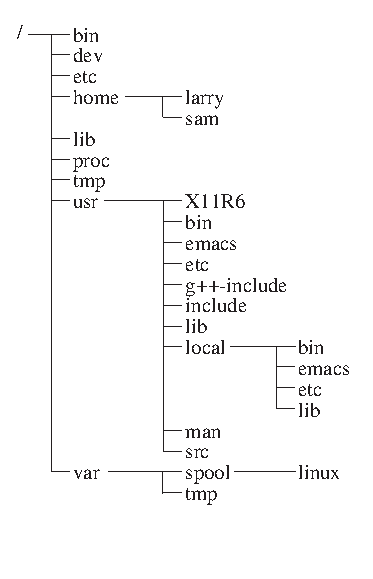
\includegraphics{tutorial/dirtree}}
\label{dirtree}
%\caption{A typical (abridged) {\linux} directory tree.}
\caption{Un t�pico �rbol de directorio {\linux} (resumido).}
\end{figure} } \fi % Kill dirtree if ASCII.

\subsection{Directorio de trabajo actual}
\index{directorio!de trabajo actual!definici�n}
\index{directorio de trabajo!definici�n}
En cualquier momento, se asume que los �rdenes que introduce se refieren a su {\bf directorio de trabajo actual}. Puede entender directorio de trabajo como el directorio en el que ''se encuentra'' 
en ese momento. Cuando accede por primera vez al sistema, su directorio de trabajo se configura como su directorio de usuario ---{\tt /home/larry}, en nuestro caso. Cuando haga referencia a un fichero,
puede referirse a �l en relaci�n a su directorio de trabajo actual, en vez de especificar el nombre de la ruta completa del fichero.

Aqu� tenemos un ejemplo. Larry tiene el directorio {\tt papers}, y {\tt papers} contiene el fichero {\tt history-final}. Si Larry quiere ver el contenido de este fichero, puede usar la orden

\begin{tscreen}
/home/larry\# more /home/larry/papers/history-final
\end{tscreen}

La orden {\tt more} simplemente muestra por pantalla un fichero, pantalla a pantalla. Como el directorio de trabajo actual de Larry es {\tt /home/larry}, se puede referir al fichero {\em en relaci�n\/} con su localizaci�n actual usando la orden

\begin{tscreen}
/home/larry\# more papers/history-final
\end{tscreen}

\index{ruta!relativa}
Si comienza el nombre del fichero (como {\tt papers/final}) con un car�cter diferente de {\tt /}, se est� refiriendo al fichero en t�rminos relativos a su directorio de trabajo actual. Esto se conoce como {\bf nombre de ruta relativo}.

\index{ruta!completa}
\index{ruta!absoluta}
Por otra parte, si comienza el nombre del fichero con una {\tt /}, el sistema lo interpreta como el nombre de la ruta absoluta ---es decir, un nombre de ruta que incluye la ruta completa hasta el fichero, comenzando en el directorio ra�z, {\tt /}. Esto se conoce como {\bf nombre de ruta absoluta}.

\subsection{Refiri�ndose al directorio inicial}
\index{directorio!inicial!\~ para referirse a@{\tt \~{}} para referise a}
\index{\~@{\tt \~{}}!para referirse al directorio inicial}
\index{home}
\index{directorio inicial}
\index{tilde}
\index{virgulilla}
Bajo {\tt tcsh} y {\tt bash}\footnote {{\tt tcsh} y {\tt bash} son dos {\em int�rprete de �rdeness} que funcionan bajo {\linux}. 
El int�rprete de �rdenes es un programa que lee los �rdenes del usuario y los ejecuta; la mayor�a de los sistema {\linux} habilitan 
{\tt tcsh} o {\tt bash} para las cuentas de los nuevos usuarios.}
puede especificar su directorio de usuario con el car�cter de la virgulilla\NT{tilde en ingl�s} ({\tt \~{}}). Por ejemplo, la orden

\begin{tscreen}
/home/larry\# more \~{}/papers/history-final
\end{tscreen}

es equivalente a

\begin{tscreen}
/home/larry\# more /home/larry/papers/history-final
\end{tscreen}

El int�rprete de �rdenes reemplaza el car�cter {\tt \~{}} por el nombre de su directorio de trabajo. 

Puede especificar tambi�n los directorios de usuario de otros usuarios con el car�cter virgulilla. La ruta {\tt \~{}karl/letters} es expandido
a {\tt /home/karl/letters} por el int�rprete de �rdenes (si {\tt /home/karl} es el directorio de usuario de Karl). El uso de la virgulilla es simplemente un atajo; no existe ning�n directorio llamado {\tt \~{}}---es s�lo una ayuda proporcionada por el int�rprete de �rdenes.

\index{{\linux}!conceptos b�sicos|)}

% Linux Installation and Getting Started    -*- TeX -*-
% basic.tex
% Copyright (c) 1992, 1993 by Matt Welsh, Larry Greenfield and Karl Fogel
%
% This file is freely redistributable, but you must preserve this copyright 
% notice on all copies, and it must be distributed only as part of "Linux 
% Installation and Getting Started". This file's use is covered by
% the copyright for the entire document, in the file "copyright.tex".
%
% Copyright (c) 1998 by Specialized Systems Consultants Inc. 
% <ligs@ssc.com>
%Revision 1 realizada el 9 de julio de 2002 por Fco. Javier Fernandez <serrador@arrakis.es>
%Revisi�n 2 Realizada el 17 de julio 2002 por Francisco Javier Fern�ndez <serrador@arrakis.es>

%\section{First steps into Linux.}
\section{Primeros Pasos en {\linux}}
\markboth{Tutorial {\linux }}{Primeros pasos en {\linux}}
Antes de que empecemos, es importante saber que todos 
los nombres de ficheros y �rdenes en un sistema {\linux} 
son {\bf case-sensitive} (que diferencian entre 
may�sculas y min�sculas a diferencia de sistemas 
operativos como MS-DOS). Por ejemplo, la orden {\tt make} 
es muy diferente de {\tt Make} o {\tt MAKE}. Lo mismo se 
cumple para nombres de ficheros y directorios.


\subsection{Movi�ndonos por la estructura de directorios.}
%\subsection{Moving around.}
Ahora que puede entrar en el sistema y que sabe c�mo referenciar los ficheros usando las rutas de los mismos, �c�mo puede cambiar el directorio de trabajo actual, para hacer la vida m�s f�cil?

\index{directorio!estructura!movi�ndose por ella con cd@movi�ndose por ella con cd {\tt cd}}
\index{cd@{\tt cd}|(}
La orden para moverse por la estructura de directorios es {\tt cd}, que es una abreviatura de ''cambiar directorio''.
Muchas de las �rdenes m�s usadas en {\linux} son de dos o tres letras.
La forma de usar la orden {\tt cd} es

\begin{tscreen}
cd \cparam{directorio}
\end{tscreen}

donde  \textsl{directorio} es el nombre del directorio que quiere que se convierta en el directorio de trabajo actual. 

Como se mencion� antes, cuando entra en el sistema, comienza en su directorio de usuario. Si Larry quisiera cambiar al subdirectorio {\tt papers}, usar�a la orden

\begin{tscreen}
/home/larry\# cd papers \\
/home/larry/papers\#
\end{tscreen}

Como puede ver, el indicador de Larry cambia para reflejar 
su directorio de trabajo actual (de forma que sabe d�nde 
se encuentra). Ahora que est� en el directorio  {\tt papers}, 
puede ver history-final con la orden

\begin{tscreen}
/home/larry/papers\# more history-final
\end{tscreen}

\index{directorio!padre!.. para referirse al@{\tt ..} para referirse al}
\index{directorio!. para referirse al@{\tt .} para referirse al}
\index{directorio padre!.. para referirse a@{\tt ..} para referirse a}

Ahora, Larry est� atascado en el subdirectorio {\tt papers}. Para regresar al directorio superior (o padre), ejecute la orden 

\begin{tscreen}
/home/larry/papers\# cd \ .. \\
/home/larry\#
\end{tscreen}

(Observe los espacios entre ``{\tt cd}'' y ``{\tt ..}''.)
Cada directorio tiene una entrada llamada ``{\tt ..}'' que se refiere al directorio padre. De forma similar, cada directorio tiene una entrada llamada ``{\tt .}''que se refiere a s� mismo. Por tanto, la orden 

\begin{tscreen}
/home/larry/papers\# cd \ .
\end{tscreen}

no lleva a ninguna parte. 

Con la orden {\tt cd} se pueden usar tambi�n rutas absolutas.
Para  cambiar  al directorio de usuario de Karl, se puede usar la orden

\begin{tscreen}
/home/larry/papers\# cd /home/karl \\
/home/karl\#
\end{tscreen}

Adem�s, la orden {\tt cd} sin argumentos le llevar� a su propio directorio de usuario. 

\begin{tscreen}
/home/karl\# cd \\
/home/larry\#
\end{tscreen}

\index{cd@{\tt cd}|)}
%\subsection{Looking at the contents of directories.}
\subsection{Mirando el contenido de los directorios}
\label{sec-ls}
\index{directorio!listar los contenidos de|(}
\index{ls@{\tt ls}|(}
\index{listando los contenidos de(}
\index{ficheros!listado|(}

Ahora que sabe c�mo moverse por los directorios, podr�a pensar, �y qu�?. Dar vueltas por los directorios no tiene mucho sentido por s� mismo, as� que introduzcamos una orden nueva,
 {\tt ls}. La orden {\tt ls} muestra un listado de ficheros y directorios, por omisi�n del directorio actual. Por ejemplo:

\begin{tscreen}
/home/larry\# ls \\
Mail \\
letters \\
papers \\
/home/larry\#
\end{tscreen}

Aqu� podemos darnos cuenta de que Larry tiene tres entradas en su directorio actual:  {\tt Mail}, {\tt letters}, y {\tt papers}. Esto no nos dice mucho -- ?` qu� son, directorios o ficheros? 
Podemos usar la opci�n {\tt -F} de la orden {\tt ls} para obtener informaci�n m�s detallada.

\begin{tscreen}
/home/larry\# ls\ --F \\
Mail/ \\
letters/ \\
papers/ \\
/home/larry\#
\end{tscreen}


Por la {\tt /} que aparece en cada nombre, sabemos que estas tres entradas son, de hecho, subdirectorios.

\index{ejecutable!definici�n}
\index{fichero!ejecutable!definici�n}

Ejecutando {\tt ls -F} puede tambi�n aparecer un ``{\tt *}'' al final de un nombre en la lista resultante, lo que indicar�a que el fichero es un {\bf ejecutable} o un programa que puede ejecutarse. 
Si no aparece nada al final de un nombre al usar {\tt ls -F}, el fichero es un ``plain old file'', es decir, no es ni un directorio ni un ejecutable.  

En general, cada orden UNIX puede tomar un cierto n�mero de opciones adem�s de otros argumentos. Estas opciones normalmente comienzan con un ``{\tt -}'', como se vi� arriba con la opci�n {\tt -F}.
 La opci�n {\tt -F} le dice a  {\tt ls} que d� m�s informaci�n acerca del tipo de ficheros involucrados --en nuestro caso, imprimiendo una {\tt /} despu�s de cada nombre de directorio. 

Si le da a {\tt ls} el nombre de un directorio, el sistema listar� los contenidos de ese directorio. 

\begin{tscreen}
/home/larry\# ls\ --F papers \\
english-lit \\
history-final \\
masters-thesis \\
notes/ \\
/home/larry\#
\end{tscreen}

O, para un listado m�s interesante, veamos qu� hay en el directorio de sistema {\tt /etc}. 

\begin{tscreen}
/home/larry\# ls /etc 
\begin{verbatim}
Images          ftpusers        lpc             rc.new          shells
adm             getty           magic           rc0.d           startcons
bcheckrc        gettydefs       motd            rc1.d           swapoff
brc             group           mount           rc2.d           swapon
brc~            inet            mtab            rc3.d           syslog.conf
csh.cshrc       init            mtools          rc4.d           syslog.pid
csh.login       init.d          pac             rc5.d           syslogd.reload
default         initrunlvl      passwd          rmt             termcap
disktab         inittab         printcap        rpc             umount
fdprm           inittab.old     profile         rpcinfo         update
fstab           issue           psdatabase      securetty       utmp
ftpaccess       lilo            rc              services        wtmp
/home/larry#
\end{verbatim}\end{tscreen}

Si es un usuario de MS-DOS, puede que se d� cuenta de que los nombres de ficheros pueden ser mayores de 8 caracteres, y pueden contener puntos en cualquier posici�n. 
Puede incluso usar m�s de un punto en un nombre de fichero.

Vayamos a la parte superior del �rbol de directorios, y luego bajemos a otro directorio con las �rdenes

\begin{tscreen}
/home/larry\# cd .. \\
/home\# cd .. \\
/\# cd usr \\
/usr\# cd bin \\
/usr/bin\#
\end{tscreen}

Puede tambi�n moverse a los directorio en un s�lo paso, haciendo {\tt cd /usr/bin}.

Pruebe a moverse por varios directorios, usando {\tt ls} y {\tt cd}. 
En algunos casos, puede que le aparezca el mensaje de error ``{\tt Permission denied}''\NT{Permiso denegado}. Esto es debido simplemente ``al sistema de seguridad UNIX'':
para poder usar las �rdenes {\tt ls} o {\tt cd}, debe tener permisos para hacerlo. Hablaremos m�s acerca de esto en
 \index{directorio!listado de los contenidos de|)}
 \index{ls@{\tt ls}|)}
 \index{listando los contenidos del directorio|)}
 \index{ficheros!listado|)}
la pagina~\pageref{sec-file-perms}.

%\subsection{Creating new directories.}
\subsection{Creaci�n de directorios nuevos}

\index{directorio!creaci�n}
\index{mkdir@{\tt mkdir}}
Es hora de aprender c�mo crear directorios. Esto requiere el uso de la orden {\tt mkdir}. Pruebe lo siguiente:

\begin{tscreen}
/home/larry\# mkdir foo \\
/home/larry\# ls -F \\
Mail/ \\
foo/ \\
letters/ \\
papers/ \\
/home/larry\# cd foo \\
/home/larry/foo\# ls \\
/home/larry/foo\# 
\end{tscreen}

!`Felicidades! Ha creado un nuevo directorio y se ha metido en �l. Como no hay 
ficheros en este nuevo directorio, aprendamos c�mo copiar ficheros de un lugar a otro.

%\subsection{Copying files.}
\subsection{Copiando ficheros}

\index{ficheros!copiar}
\index{copiar ficheros}
\index{cp@{\tt cp}}

Para copiar ficheros, use el orden {\tt cp}, como se muestra aqu�:

\begin{tscreen}
/home/larry/foo\# cp /etc/termcap\ \ . \\
/home/larry/foo\# cp /etc/shells\ \ . \\
/home/larry/foo\# ls\ --F \\
shells\ \ \ \ \ termcap  \\
/home/larry/foo\# cp shells bells \\
/home/larry/foo\# ls\ --F \\
bells\ \ \ \ \ shells\ \ \ \ \ termcap \\
/home/larry/foo\# 
\end{tscreen}

La orden {\tt cp} copia los ficheros escritos en la l�nea de �rdenes al fichero o directorio dados como �ltimo argumento. D�se cuenta de que usamos``{\tt .}'' para referirnos al directorio 
actual.

%\subsection{Moving files.}
\subsection{Moviendo ficheros}
\index{fichero!mover}
\index{mover ficheros}
\index{mv@{\tt mv}}

El orden {\tt mv} mueve ficheros, en vez de copiarlos. 
La sintaxis es muy parecida:

\begin{tscreen}
/home/larry/foo\# mv termcap sells \\
/home/larry/foo\# ls -F \\
bells\ \ \ \ \ sells\ \ \ \ \ shells \\
/home/larry/foo\# 
\end{tscreen}

D�se cuenta de que el fichero {\tt termcap} ha sido renombrado a {\tt shells}. Puede adem�s usar la orden {\tt mv} para mover un fichero a un directorio completamente 
nuevo.

\blackdiamond {\bf Nota:} {\tt mv} y {\tt cp} sobreescribir�n un fichero de destino que tiene el mismo nombre sin pregunt�rselo. Tenga cuidado cuando mueva un fichero a otro directorio. Puede que haya un fichero con el mismo nombre en ese directorio, !`que ser� sobreescrito!

%\subsection{Deleting ficheros and directories.}
\subsection{Borrando ficheros y directorios}
\index{fichero!borrar}
\index{borrar!ficheros}
\index{rm@{\tt rm}}
Usted tiene ahora una fea rima, que ha creado usando el orden {\tt ls}.
Para borrar un fichero, use el orden {\tt rm}, que proviene de ''remove'',\NT{quitar} como se muestra aqu�:

\begin{tscreen}
/home/larry/foo\# rm bells sells \\
/home/larry/foo\# ls -F \\
shells \\
/home/larry/foo\#
\end{tscreen}

No nos queda nada salvo shells, pero no nos quejaremos. D�se cuenta de que {\tt rm} no 
le preguntar� antes de borrar un fichero, as� que tenga cuidado.

\index{borrar!directorio}
\index{directorio!borrar}
\index{rmdir@{\tt rmdir}}
Una orden relacionada con {\tt rm} es {\tt rmdir}. Este orden borra un directorio, pero s�lo si 
el directorio est� vac�o. Si el directorio contiene alg�n fichero o 
subdirectorio, {\tt rmdir} protestar�.

%\subsection{Looking at ficheros.}
\subsection{Mirando en los ficheros}
\index{ficheros!ver el contenido de}
\index{more@{\tt more}}
\index{cat@{\tt cat}!para ver el contenido de un fichero}
Las �rdenes {\tt more} y {\tt cat} se usan para ver el contenido de los ficheros. El orden {\tt more} muestra un fichero, una pantalla completa cada vez, mientras que {\tt cat} muestra el fichero completo de una vez.

Para ver el contenido del fichero {\tt shells}, use la orden

\begin{tscreen}
/home/larry/foo\# more shells
\end{tscreen}

En caso de que est� interesado en lo que contiene {\tt shells}, es una lista de int�rpretes de �rdenes (shell) v�lidos en su sistema. En la mayor�a de los sistemas, esto incluye {\tt /bin/sh}, {\tt /bin/bash} y {\tt /bin/csh}. Hablaremos acerca de estos diferentes tipos de int�rpretes de �rdenes m�s adelante.

Mientras est� usando {\tt more}, presione \key{Space} para ver la siguiente p�gina de texto, y \key{b} para ver la p�gina anterior. Hay otras �rdenes disponibles en {\tt more},
�stos son s�lo los b�sicos. Podr� salir de {\tt more} pulsando \key{q}.

Salga de {\tt more} y pruebe {\tt cat /etc/termcap}. Probablemente el texto ir� demasiado r�pido para que pueda leerlo. 
El nombre ``{\tt cat}'' proviene de hecho de ``concatenate'', que es el verdadero uso del programa. El orden {\tt cat} puede usarse para "encadenar" los contenidos de varios ficheros y guardar el
 resultado en otro fichero.
Volveremos a esto en la secci�n ~\ref{sec-shell-script}.

%\subsection{Getting online help.}
\subsection{Obteniendo ayuda en l�nea}


\index{{\linux}!p�ginas de manual para}
\index{ayuda!en l�nea}
\index{p�ginas del manual}
\index{maunal de linux}
Casi todos los sistemas UNIX, incluyendo {\linux}, facilitan lo que se conoce como {\bf p�ginas del manual}. Estas p�ginas contienen documentaci�n acerca de �rdenes del sistema, recursos, ficheros
 de configuraci�n, etc.

\index{man@{\tt man}}

La orden usada para acceder a las p�ginas del manual es {\tt man}. Si est� interesado en aprender nuevas opciones de la orden {\tt ls} puede escribir

\begin{tscreen}
/home/larry\# man ls
\end{tscreen}

y se mostrar� la p�gina del manual para {\tt ls}.

Por desgracia, la mayor�a de las p�ginas de manual est�n escritas por personas que ya tienen alguna idea de lo que la orden o recurso hace. Por esta raz�n, las p�ginas del manual, a menudo,
 contienen s�lo los detalles t�cnicos de la orden, sin mucha explicaci�n. De todos modos, las p�ginas del manual pueden constituir un recurso muy valioso para refrescar su memoria si se le 
olvida la sintaxis de una orden. Las p�ginas del manual le hablar�n adem�s de �rdenes que no veremos en este libro.

Sugiero que pruebe {\tt man} para las �rdenes que ya hemos visto y cuando
veamos alguno nuevo. Algunas de estas �rdenes no tendr�n p�gina de manual,
por distintas razones. Primero, las p�ginas de manual puede que no se hayan
escrito todav�a. El proyecto de documentaci�n de {\linux} tambi�n es responsable de
las p�ginas de manual de {\linux}. Estamos acumulando poco a poco la
mayor�a de las p�ginas de manual disponibles para el sistema). Segundo, la
orden podr�a ser una orden interna del shell, o un alias (que se
discutir� en la p�gina ~\pageref{sec-shells-cmds}), la cual podr�a no tener
una p�gina de manual propia. Un ejemplo es {\tt cd}, que es una orden
interna del shell. El shell por s� s�lo procesa la orden {\tt cd} --- 
no hay un programa separado que implemente esta orden.

% {\linux} Installation and Getting Started    -*- TeX -*-
% msdos.tex
% Copyright (c) 1992, 1993 by Matt Welsh <mdw@sunsite.unc.edu>
%
% This file is freely redistributable, but you must preserve this copyright 
% notice on all copies, and it must be distributed only as part of "{\linux} 
% Installation and Getting Started". This file's use is covered by the 
% copyright for the entire document, in the file "copyright.tex".
%
% Copyright (c) 1998 by Specialized Systems Consultants Inc. 
% <ligs@ssc.com>

%\section{Accessing MS-DOS files.}
\section{Acceder a los ficheros MS-DOS\TM}
\markboth{Caracter�sticas Avanzadas}{Acceso a ficheros MS-DOS\tm}
\label{sec-msdos-mount}
\index{MS-DOS!acceder ficheros desde}
\index{ficheros!MS-DOS}
Si, por cualquier retorcida y extrafalaria raz�n, quiere acceder a ficheros
de MS-DOS, lo  podr� hacer f�cilmente desde {\linux}.

\index{MS-DOS!montando una partici�n bajo {\linux}}
\index{mount@{\tt mount}!para montar una partici�n MS-DOS}
La manera normal de acceder a los ficheros de MS-DOS es montar una partici�n MS-DOS o
un disco flexible bajo {\linux}, lo cual permite acceder a los ficheros directamente a trav�s
del sistema de ficheros. Por ejemplo, si tiene un disco flexible MS-DOS en
{\tt /dev/fd0}, la orden

\begin{tscreen}
\# mount -t msdos /dev/fd0 /mnt
\end{tscreen}

lo montar� en {\tt /mnt}. Consulte la Secci�n~\ref{sec-floppy} para m�s
informaci�n sobre c�mo montar discos flexibles.

Tambi�n puede montar una partici�n MS-DOS de su disco duro para que sea
accesible desde {\linux}. Si tiene una partici�n MS-DOS en {\tt /dev/hda1}, la orden

\begin{tscreen}
\# mount -t msdos /dev/hda1 /mnt
\end{tscreen}

la monta. Aseg�rese de desmontar ({\tt umount}) la partici�n cuando haya terminado
de usarla. Tambi�n se puede hacer que una partici�n MS-DOS se monte autom�ticamente
en el momento del arranque si incluye la entrada en {\tt /etc/fstab}. Consulte la
Secci�n~\ref{sec-manage-fs} para m�s detalles. La siguiente l�nea en {\tt
/etc/fstab} monta una partici�n MS-DOS en {\tt /dev/hda1} en el
directorio {\tt /dos}.

\begin{tscreen}
/dev/hda1\ \ \ \ \ /dos\ \ \ \ \ msdos \ \ \ \ \ defaults
\end{tscreen}

Tambi�n puede montar los sistemas de ficheros VFAT usados por Windows 95 y 98:

\begin{tscreen}
\# mount -t vfat /dev/hda1 /mnt
\end{tscreen}

Esto permite acceder a los nombres largos de ficheros de Windows 95\tm. Esto s�lo
se aplica a particiones que realmente tengan almacenados los nombres en formato
largo. No se puede montar un sistema de ficheros FAT16 normal y usarlo para
obtener nombres de ficheros largos.

\index{MS-DOS!uso de Mtools para acceder a ficheros}
El software Mtools tambi�n puede ser usado para acceder a ficheros MS-DOS\tm. Las
�rdenes {\tt mcd}, {\tt mdir}, y {\tt mcopy} se comportan todas como sus
equivalentes MS-DOS\tm. Si instala las Mtools, deber�a tener p�ginas del manual
disponibles para estas �rdenes.

\index{MS-DOS!ejecuci�n de programas bajo {\linux}}
\index{MS-DOS!emulador}
\index{Microsoft Windows!emulador} 
Acceder a ficheros MS-DOS es una cosa; ejecutar programas MS-DOS es
otra. Hay un emulador de MS-DOS\tm en desarrollo para {\linux}; es
f�cil de conseguir, y est� inclu�do en la mayor�a de las distribuciones.
Tambi�n se puede conseguir en muchos sitios, incluyendo los sitios
FTP para {\linux} listados en el Ap�ndice~\ref{app-ftp}. El emulador de MS-DOS est�
considerado como lo suficientemente potente para hacer funcionar un buen n�mero de
aplicaciones, incluyendo Wordperfect\tm, desde {\linux}. Sin embargo, {\linux} y MS-DOS son
sistemas operativos marcadamente diferentes. La potencia de cualquier emulador de MS-DOS
bajo UNIX est� limitada. Adem�s, est� en desarrollo un emulador de Microsoft Windows
que corra bajo X Window.











% \linux Installation and Getting Started    -*- TeX -*-
% commands.tex
% Copyright (c) 1992, 1993 by Matt Welsh, Larry Greenfield and Karl Fogel
%
% This fichero is freely redistributable, but you must preserve this copyright 
% notice on all copies, and it must be distributed only as part of "\linux 
% Installation and Getting Started". This fichero's use is covered by
% the copyright for the entire document, in the fichero "copyright.tex".
%
% Copyright (c) 1998 by Specialized Systems Consultants Inc. 
% <ligs@ssc.com>
% Revisi�n 1 por Fco. Javer Fern�ndez <serrador@arrakis.es> 9 de julio del 2002
%
%\section{Summary of basic UNIX commands.}\label{sec-command-summ}
\section{Sumario de �rdenes b�sicas}
\label{sec-command-summ}
\markboth{Tutorial de {\linux}}{Sumario de �rdenes b�sicas UNIX}

\index{�rdenes!sumario de b�sicas|(}
Esta secci�n introduce algunas de las m�s �tiles �rdenes b�sicas de un sistema UNIX, incluyendo aqu�llas que son cubiertas en la secci�n anterior.

\index{�rdenes!-@{\tt -} flag de opci�n de orden}
\index{flag@{\tt -} de opci�n de orden}
F�jese en que las opciones suelen empezar con ``{\tt -}'', y en la mayor�a de los casos es posible especificar m�s de una opci�n con un �nico ``{\tt -}''. Por ejemplo, en vez de usar {\tt ls -l -F}, 
se puede escribir {\tt ls -lF}.

En lugar de dar una lista de cada una de las opciones de una orden, ahora s�lo vamos a presentar �rdenes �tiles o importantes. De hecho, la mayor�a de estas �rdenes tienen muchas opciones 
que nunca usar�. Puede usar {\tt man} para echar un vistazo a las p�ginas de manual de cada orden, el cu�l lista todas las opciones disponibles.

D�se cuenta tambi�n de que muchas de estas �rdenes toman como argumento una lista de ficheros o directorios, indicados en esta tabla por ``\textsl{fichero1} \ldots \textsl{ficheroN}''. Por ejemplo,
la orden {\tt cp} toma como argumentos una lista de ficheros para copiar, seguido del fichero o directorio destino. Cuando va a copiar m�s de un fichero, el destino debe ser un directorio.

\begin{dispitems}

\index{cd@{\tt cd}}
\ditem {{\tt cd}}
Cambia el directorio de trabajo actual \\
Sintaxis: {\tt cd \cparam{directorio}} \\
Donde \textsl{directorio} es el directorio al que se quiere cambiar. ``{\tt .}''
hace referencia al directorio actual, ``{\tt ..}'' al directorio padre. Si no se especifica ning�n directorio le lleva, por omisi�n, a su directorio de usuario. \\

Ejemplo: {\tt cd ../foo} sube el directorio actual un nivel, y entonces, se introduce en el directorio {\tt foo}.

\index{ls@{\tt ls}}
\ditem {{\tt ls}}
Muestra informaci�n acerca de los ficheros y directorios nombrados. \\
Sintaxis: {\tt ls \cparam{ficheros} }\\
Donde \textsl{ficheros} consiste en los nombres de ficheros o directorios que se quieren listar. Las opciones que m�s se usan son {\tt -F} (para mostrar el tipo de fichero) y {\tt -l}
 (para mostrar una lista ''ampliada'' incluyendo el tama�o de los ficheros, propietario, permisos, etc.). \\
Ejemplo: {\tt ls -lF /home/larry} muestra los contenidos del directorio {\tt /home/larry}.

\index{cp@{\tt cp}}
\ditem {{\tt cp}} 
Copia uno o m�s ficheros a otro fichero o directorio. \\
Sintaxis: {\tt cp \cparam{ficheros}
\cparam{destino}} \\
Donde \textsl{ficheros} indica los ficheros que hay que copiar, y
\textsl{destino} es el fichero o directorio destino. \\

Ejemplo: {\tt cp ../frog joe} copia el fichero {\tt ../frog} al fichero o directorio {\tt joe}.

\index{mv@{\tt mv}}
\ditem {{\tt mv}} 
Mueve uno o m�s ficheros a otro directorio. Esta orden hace el equivalente de una copia seguido del borrado del fichero original.
Puede usar esto para renombrar ficheros, como con la orden de MS-DOS {\tt RENAME}. \\
Sintaxis: {\tt mv \cparam{ficheros}
\cparam{destino}} \\
Donde \textsl{ficheros} indica los arhivos que hay que mover, y
\textsl{destino} es el fichero o directorio destino. \\

Ejemplo: {\tt mv ../frog joe} mueve el fichero {\tt ../frog} al fichero o directorio {\tt joe}.

\index{rm@{\tt rm}}
\ditem {{\tt rm}} 
Borra ficheros. F�jese en que cuando borra un fichero bajo UNIX, 
son irrecuperables (al contrario que con MS-DOS, donde normalmente se puede ''desborrar'' el fichero). \\
Sintaxis: {\tt rm \cparam{ficheros}} \\
Donde \textsl{ficheros} describe el nombre de los ficheros que hay que borrar. \\
La opci�n {\tt -i} le pide confirmaci�n antes de borrar el fichero. \\

Ejemplo: {\tt rm -i /home/larry/joe /home/larry/frog} borra los ficheros {\tt joe} y {\tt frog} en {\tt /home/larry}.


\index{mkdir@{\tt mkdir}}
\ditem {{\tt mkdir}}
Crea nuevos directorios.\\
Sintaxis: {\tt mkdir \cparam{dirs} }\\
Donde \textsl{dirs} son los directorios que hay que crear. \\

Ejemplo: {\tt mkdir /home/larry/test} crea el directorio {\tt test}
en {\tt /home/larry}.

\index{rmdir@{\tt rmdir}}
\ditem {{\tt rmdir}} 
Borra directorios vac�os. Cuando use {\tt rmdir}, el directorio de trabajo actual no debe estar dentro del directorio que se pretende borrar. \\
Sintaxis: {\tt rmdir \cparam{dirs} }\\
Donde \textsl{dirs} define los directorios que hay que borrar. \\

Ejemplo: {\tt rmdir /home/larry/papers} borra el directorio {\tt /home/larry/papers}, si est� vac�o. 

\index{man@{\tt man}}
\ditem {{\tt man}} 
Muestra la p�gina de manual para la orden o recurso dado (es decir, no una utilidad del sistema que no sea 
una orden, como una funci�n de biblioteca.)\\

Sintaxis: {\tt man \cparam{command}} \\

Donde \textsl{command} es el nombre de la orden o recurso del que se quiere conseguir ayuda.\\

Ejemplo: {\tt man ls} le da informaci�n acerca de la orden {\tt ls}.

\index{more@{\tt more}}
\ditem {{\tt more}} 
Muestra informaci�n del contenido de los ficheros nombrados, pantalla por pantalla. \\
Sintaxis: {\tt more \cparam{ficheros}} \\
Donde \textsl{ficheros} indica los ficheros que se quieren mostrar. \\

Ejemplo: {\tt more papers/history-final} muestra el fichero {\tt papers/history-final}.

\index{cat@{\tt cat}}
\ditem {{\tt cat}} 
Oficialmente usado para concatenar ficheros, {\tt cat} tambi�n se usa para mostrar los contenidos de un fichero por pantalla. \\
Sintaxis: {\tt cat \cparam{ficheros}} \\
Donde \textsl{ficheros} indica los ficheros que se quieren mostrar. \\

Ejemplo: {\tt cat letters/from-mdw} muestra el fichero {\tt letters/from-mdw}.

\index{echo@{\tt echo}}
\ditem{{\tt echo}}
Muestra en la pantalla los argumentos que se le pasan a la orden. \\
Sintaxis: {\tt echo \cparam{args}} \\
Donde \textsl{args} indica los argumentos que se quieren mostrar. \\

Ejemplo: {\tt echo ``Hello world''} muestra la cadena ``{\tt Hello world}''.

\index{grep@{\tt grep}}
\ditem{{\tt grep}}
Muestra cada l�nea en uno o m�s ficheros que contiene un patr�n dado. \\
Sintaxis: {\tt grep \cparam{pattern} \cparam{ficheros}} \\
Donde \textsl{pattern} es un patr�n, y 
\textsl{ficheros} indica los ficheros donde se quiere buscar dicho patr�n. \\

Ejemplo: {\tt grep loomer /etc/hosts} muestra cada l�nea en el fichero {\tt /etc/hosts} que contiene el patr�n ``{\tt loomer}''.

\end{dispitems}

\index{�rdenes!sumario de las b�sicas|)}




\chapter{El sistema de archivos}
\label{filesystem-chapter}

\ChapterDescription{Este capitulo describe c�mo el kernel de Linux
  gestiona los ficheros en los sistemas de ficheros soportados por
  �ste.  Describe el Sistema de Ficheros Virtual (VFS) y explica c�mo
  los sistemas de ficheros reales del kernel de Linux son soportados.}

\index{File system} Una de los rasgos m�s importantes de Linux es su
soporte para diferentes sistemas de ficheros.  �sto lo hace muy
flexible y bien capacitado para coexistir con muchos otros sistemas
operativos.  En el momento de escribir �sto, Linux soporta 15 sistemas
de ficheros; \texttt{ext}, \texttt{ext2}, \texttt{xia},
\texttt{minix}, \texttt{umsdos}, \texttt{msdos}, \texttt{vfat},
\texttt{proc}, \texttt{smb}, \texttt{ncp}, \texttt{iso9660},
\texttt{sysv}, \texttt{hpfs}, \texttt{affs} and \texttt{ufs}, y sin
duda, con el tiempo se a�adir�n m�s.

En Linux, como en Unix\tm, a los distintos sistemas de ficheros que el
sistema puede usar no se accede por identificadores de dispositivo
(como un n�mero o nombre de unidad) pero, en cambio se combinan en una
simple structura jer�rquica de �rbol que representa el sistema de
ficheros como una entidad �nica y sencilla.  Linux a�ade cada sistema
de ficheros nuevo en este simple �rbol de sistemas de ficheros cuando
se monta.  Todos los sistemas de ficheros, de cualquier tipo, se
montan sobre un directorio y los ficheros del sistema de ficheros son
el contenido de ese directorio.  Este directorio se conoce como
directorio de montaje o punto de montaje.  Cuando el sistema de
ficheros se desmonta, los ficheros propios del directorio de montaje
son visibles de nuevo.

Cuando se inicializan los discos (usando \eg{fdisk}, por ejemplo)
tienen una estructura de partici�n inpuesta que divide el disco f�sico
en un n�mero de particiones l�gicas.  Cada partici�n puede mantener un
sistema de ficheros, por ejemplo un sistema de ficheros \texttt{EXT2}.
Los sistemas de ficheros organizan los ficheros en structuras
jer�rquicas l�gicas con directorios, enlaces flexibles y m�s
contenidos en los bloques de los dispositivos f�sicos.  Los
dispositivos que pueden contener sistemas de ficheros se conocen con
el nombre de dispositivos de bloque.  La partici�n de disco IDE
\fn{/dev/hda1}, la primera partici�n de la primera unidad de disco en
el sistema, es un dispositivo de bloque.  Los sistemas de ficheros de
Linux contemplan estos dispositivos de bloque como simples colecciones
lineales de bloques, ellos no saben o tienen en cuenta la geometr�a
del disco f�sico que hay debajo.  Es la tarea de cada controlador de
dispositivo de bloque asignar una petici�n de leer un bloque
particular de su dispositivo en t�rminos comprensibles para su
dispositivo; la pista en cuesti�n, sector y cilindro de su disco duro
donde se guarda el bloque.  Un sistema de ficheros tiene que mirar,
sentir y operar de la misma forma sin importarle con que dispositivo
est� tratando.  Por otra parte, al usar los sistemas de ficheros de
Linux, no importa (al menos para el usuario del sistema) que estos
distintos sistemas de ficheros est�n en diferentes soportes
controlados por diferentes controladores de hardware.  El sistema de
ficheros puede incluso no estar en el sistema local, puede ser
perfectamente un disco remoto montado sobre un enlace de red.
Considerese el siguiente ejemplo donde un sistema Linux tiene su
sistema de ficheros ra�z en un disco SCSI:
\begin{verbatim}
A         E         boot      etc       lib       opt       tmp       usr
C         F         cdrom     fd        proc      root      var       sbin
D         bin       dev       home      mnt       lost+found
\end{verbatim}
Ni los usuarios ni los programas que operan con los ficheros necesitan
saber que \fn{/C} de hecho es un sistema de ficheros VFAT montado que
est� en el primer disco IDE del sistema.  En el ejemplo (que es mi
sistema Linux en casa), \fn{/E} es el disco IDE primario en la segunda
controladora IDE.  No importa que la primera controladora IDE sea una
controladora PCI y que la segunda sea una controladora ISA que tambi�n
controla el IDE CDROM.  Puedo conectarme a la red donde trabajo usando
un modem y el protocolo de red PPP y en este caso puedo remotamente
montar mis sistemas de ficheros Linux \axp\ sobre \fn{/mnt/remote}.

Los ficheros en un sistema de ficheros son grupos de datos; el fichero
que contiene las fuentes de este cap�tulo es un fichero ASCII llamado
\fn{filesystems.tex}.  Un sistema de ficheros no s�lo posee los datos
contenidos dentro de los ficheros del sistema de ficheros, adem�s
mantiene la estructura del sistema de ficheros.  Mantiene toda la
informaci�n que los usuarios de Linux y procesos ven como ficheros,
directorios, enlaces flexibles, informaci�n de protecci�n de ficheros
y as�.  Por otro lado debe mantener esa informaci�n de forma eficiente
y segura, la integridad b�sica del sistema operativo depende de su
sistema de ficheros.  Nadie usaria un sistema operativo que perdiera
datos y ficheros de forma aleatoria\footnote{Bueno, no con
  conocimiento, sin embargo me he topado con sistemas operativos con
  m�s abogados que programadores tiene Linux}.

\texttt{Minix}, el primer sistema de ficheros que Linux tuvo es
bastante restrictivo y no era muy r�pido.  \texttt{Minix}, the first
file system that Linux had is rather restrictive and lacking in
performance.\index{Minix} Sus nombres de ficheros no pueden tener m�s
de 14 caracteres (que es mejor que nombres de ficheros 8.3) y el
tama�o m�ximo de ficheros es 64 MBytes.  64 MBytes puede a primera
vista ser suficiente pero se necesitan tama�os de ficheros m�s grandes
para soportar incluso modestas bases de datos.  El primer sistema de
ficheros dise�ado especificamente para Linux, el sistema de Ficheros
Extendido, o \texttt{EXT}, fue introducido en Abril de 1992 y solvent�
muchos problemas pero era aun falto de rapidez.  \index{EXT}
\index{Extended File system} As�, en 1993, el Segundo sistema de
Ficheros Extendido, o \texttt{EXT2}, fue a�adido.  \index{EXT2}
\index{Second Extended File system} Este es el sistema de ficheros que
se describe en detalle m�s tarde en este cap�tulo.

Un importante desarrollo tuvo lugar cuando se a�adi� en sistema de
ficheros EXT en Linux.  El sistema de ficheros real se separ� del
sistema operativo y servicios del sistema a favor de un interfaz
conocido como el sistema de Ficheros Virtual, o VFS.  \index{VFS}
\index{Virtual File system} VFS permite a Linux soportar muchos,
incluso muy diferentes, sistemas de ficheros, cada uno presentando un
interfaz software com�n al VFS.  Todos los detalles del sistema de
ficheros de Linux son traducidos mediante software de forma que todo
el sistema de ficheros parece id�ntico al resto del kernel de Linux y
a los programas que se ejecutan en el sistema.  La capa del sistema de
Ficheros Virtual de Linux permite al usuario montar de forma
transparente diferentes sistemas de ficheros al mismo tiempo.

El sistema de Ficheros Virtual est� implementado de forma que el
acceso a los ficheros es r�pida y tan eficiente como es posible.
Tambi�n debe asegurar que los ficheros y los datos que contiene son
correctos.  Estos dos requisitos pueden ser incompatibles uno con el
otro.  El VFS de Linux mantiene una antememoria con informaci�n de
cada sistema de ficheros montado y en uso.  Se debe tener mucho
cuidado al actualizar correctamente el sistema de ficheros ya que los
datos contenidos en las antememorias se modifican cuando cuando se
crean, escriben y borran ficheros y directorios.  Si se pudieran ver
las estructuras de datos del sistema de ficheros dentro del kernel en
ejecuci�n, se podria ver los bloques de datos que se leen y escriben
por el sistema de ficheros.  Las estructuras de datos, que describen
los ficheros y directorios que son accedidos serian creadas y
destruidas y todo el tiempo los controladores de los dispositivo
estarian trabajando, buascando y guardando datos.  La antememoria o
cach� m�s importantes es el Buffer Cache, que est� integrado entre
cada sistema de ficheros y su dispositivo de bloque.  Tal y como se
accede a los bloques se ponen en el Buffer Cache y se almacenan en
varias colas dependiendo de sus estados.  El Buffer Cache no s�lo
mantiene buffers de datos, tambien ayuda a administrar el interfaz
as�ncrono con los controladores de dispositivos de bloque.

\section{The Second Extended File system (EXT2)}
\index{EXT2}
\begin{figure}
\begin{center}
{\centering \includegraphics{fs/ext2.eps} \par}
\end{center}
\caption{Physical Layout of the EXT2 File system}
\label{ext2fs-figure}
\end{figure}
El Segundo sistema de ficheros Extendido fue pensado (por R�my Card)
como un sistema de ficheros extensible y poderoso para Linux.  Tambi�n
es el sistema de ficheros m�s �xito tiene en la comunidad Linux y es
b�sico para todas las distribuciones actuales de Linux.
\SeeModule{fs/�ext2/�*} El sistema de ficheros EXT2, como muchos
sistemas de ficheros, se construye con la premisa de que los datos
contenidos en los ficheros se guarden en bloques de datos.  Estos
bloques de datos son todos de la misma longitud y, si bien esa
longitud puede variar entre diferentes sistemas de ficheros EXT2 el
tama�o de los bloques de un sistema de ficheros EXT2 en particular se
decide cuando se crea (usando \eg{mke2fs}).  El tama�o de cada fichero
se redondea hasta un numero entero de bloques.  Si el tama�o de bloque
es 1024 bytes, entonces un fichero de 1025 bytes ocupar� dos bloques
de 1024 bytes.  Desafortunadamente esto significa que en promedio se
desperdicia un bloque por fichero.
Normalmente en ordenadores se cambia la carga de CPU por m�s espacio de memoria o de disco utilizado. En este caso Linux, como muchos sistemas operativos, cambia una ineficiencia relativa en el uso del disco a cambio de reducir la carga de la CPU.

No todos los bloques del sistema de ficheros contienen datos, algunos
deben usarse para mantener la informaci�n que describe la estructura
del sistema de ficheros.  EXT2 define la topologia del sistema de
ficheros describiendo cada fichero del sistema con una estructura de
datos inodo.  Un inodo describe que bloques ocupan los datos de un
fichero y tambi�n los permisos de acceso del fichero, las horas de
modificaci�n del fichero y el tipo del fichero.  Cada fichero en el
sistema de ficheros EXT2 se describe por un �nico inodo y cada inodo
tiene un �nico n�mero que lo identifica.  Los inodos del sistema de
ficheros se almacenan juntos en tablas de inodos.  Los directorios
EXT2 son simplemente ficheros especiales (ellos mismos descritos por
inodos) que contienen punteros a los inodos de sus entradas de
directorio.

La figura�\ref{ext2fs-figure} muestra la disposici�n del sistema de
ficheros EXT2 ocupando una serie de bloques en un dispositivo
estructurado bloque.  Por la parte que le toca a cada sistema de
ficheros, los dispositivos de bloque son s�lo una serie de bloques que
se pueden leer y escribir.  Un sistema de ficheros no se debe
preocupar donde se debe poner un bloque en el medio f�sico, eso es
trabajo del controlador del dispositivo.  Siempre que un sistema de
ficheros necesita leer informaci�n o datos del dispositivo de bloque
que los contiene, pide que su controlador de dispositivo lea un n�mero
entero de bloques.  El sistema de ficheros EXT2 divide las particiones
l�gicas que ocupa en Grupos de Bloque (Block Groups).  \index{EXT2
  Block Groups} Cada grupo duplica informaci�n cr�tica para la
integridad del sistema de ficheros ya sea valiendose de ficheros y
directorios como de bloques de informaci�n y datos.  Esta duplicaci�n
es necesaria por si ocurriera un desastre y el sistema de ficheros
necesitara recuperarse.  Los subapartados describen con m�s detalle
los contenidos de cada Grupo de Bloque.

\subsection{El inodo de EXT2}
\begin{figure}
\begin{center}
{\centering \includegraphics{fs/ext2_inode.eps} \par}
\end{center}
\caption{El inodo de EXT2}
\label{ext2fs-inode-figure}
\end{figure}
\index{El inodo de EXT2} \index{Estructuras de datos, el inodo EXT2} En el sistema de ficheros \texttt{EXT2}, el inodo es el bloque de construcci�n
b�sico; cada fichero y directorio del sistema de ficheros es descrito
por un y s�lo un inodo.  Los inodos EXT2 para cada Grupo de Bloque se
almacenan juntos en la table de inodos con un mapa de bits que permite
al sistema seguir la pista de inodos reservados y libres.  La
figura�\ref{ext2fs-inode-figure} muestra el formato de un inodo EXT2,
entre otra informaci�n, contiene los siguientes campos:
\SeeModule{include/\-linux/\-ext2\_fs\_i.h}
\begin{description}
\item [mode] Esto mantiene dos partes de informaci�n; qu� inodo
  describe y los permisos que tienen los usuarios.  Para EXT2, un
  inodo puede describir un ficheros, directorio, enlace simb�lico,
  dispositivo de bloque, dispositivo de caracter o FIFO.
\item [Owner Information] Los identificadores de usuario y grupo de
  los due�os de este fichero o directorio.  Esto permite al sistema de
  ficheros aplicar correctamente el tipo de acceso,
\item [Size] El tama�o en del fichero en bytes,
\item [Timestamps] La hora en la que el inodo fue creado y la �ltima
  hora en que se modific�,
\item [Datablocks] Punteros a los bloques que contienen los datos que
  este inodo describe.  Los doce primeros son punteros a los bloques
  f�sicos que contienen los datos descritos por este inodo y los tres
  �ltimos punteros contienen m�s y m�s niveles de indirecci�n.  Por
  ejemplo, el puntero de doble indirecci�n apunta a un bloque de
  punteros que apuntan a bloques de punteros que apuntan a bloques de
  datos.  Esto significa que ficheros menores o iguales a doce bloques
  de datos en longitud son m�s facilmente accedidos que ficheros m�s
  grandes.
\end{description}
Indicar que los inodos EXT2 pueden describir ficheros de dispositivo
especiales.  No son ficheros reales pero permiten que los programas
puedan usarlos para acceder a los dispositivos.  Todos los ficheros de
dispositivo de \fn{/dev} est�n ahi para permitir a los programas
acceder a los dispositivos de Linux.  Por ejemplo el programa
\eg{mount} toma como argumento el fichero de dispositivo que el
usuario desee montar.

\subsection{El superbloque EXT2}
\index{Superbloque EXT2} El Superbloque contiene una descripci�n del
tama�o y forma base del sistema de ficheros.  La informaci�n contenida
permite al administrador del sistema de ficheros usar y mantener el
sistema de ficheros.  Normalmente s�lo se lee el Superbloque del Grupo
de Bloque 0 cuando se monta el sistema de ficheros pero cada Grupo de
Bloque contiene una copia duplicada en caso de que se corrompa sistema
de ficheros.  Entre otra informaci�n contiene el:
\SeeModule{include/\-linux/\-ext2\_fs\_sb.h}
\begin{description}
\item [Magic Number] Esto permite al software de montaje comprobar que
  es realmente el Superbloque para un sistema de ficheros EXT2.  Para
  la versi�n actual de \texttt{EXT2} �ste es \hex{EF53}.
\item [Revision Level] Los niveles de revisi�n mayor y menor permiten
  al c�digo de montaje determinar si este sistema de ficheros soporta
  o no caracter�sticas que s�lo son disponibles para revisiones
  particulares del sistema de ficheros.  Tambi�n hay campos de
  compatibilidad que ayudan al c�digo de montaje determinar que nuevas
  caracter�sticas se pueden usar con seguridad en ese sistema de
  ficheros,
\item [Mount Count and Maximum Mount Count] Juntos permiten al sistema
  determinar si el sistema de ficheros fue comprobado correctamente.
  El contador de montaje se incrementa cada vez que se monta el
  sistema de ficheros y cuando es igual al contador m�ximo de montaje
  muestra el mensaje de aviso �maximal mount count reached, running
  e2fsck is recommended�,
\item [Block Group Number] El n�mero del Grupo de Bloque que tiene la
  copia de este Superbloque,
\item [Block Size] El tama�{o} de bloque para este sistema deficheros
  en bytes, por ejemplo 1024 bytes,
\item [Blocks per Group] El n�mero de bloques en un grupo.  Como el
  tama�o de bloque �ste se fija cuando se crea el sitema de ficheros,
\item [Free Blocks] EL n�mero de bloques libres en el sistema de
  ficheros,
\item [Free Inodes] El n�mero de Inodos libres en el sistema de
  ficheros,
\item [First Inode] Este es el n�mero de inodo del primer inodo en el
  sistema de ficheros.  El primer inodo en un sistema de ficheros EXT2
  ra�z seria la entrada directorio para el directorio '/'.
\end{description}

\subsection{The EXT2 Group Descriptor}
\index{EXT2 Group Descriptor} Cada Grupo de Bloque tiene una
estructura de datos que lo describe.  Como el Superbloque, todos los
descriptores de grupo para todos los Grupos de Bloque se duplican en
cada Grupo de Bloque en caso de corrupci�n del sistema de fichero.
\SeeCode{ext2\_group\_desc}{include/\-linux/\-ext2\_fs.h} Cada
Descriptor de Grupo contiene la siguiente informaci�n:
\begin{description}
\item [Blocks Bitmap] El n�mero de bloque del mapa de bits de bloques
  reservados para este Grupo de Bloque.  Se usa durante la reseva y
  liberaci�n de bloques,
\item [Inode Bitmap] El n�mero de bloque del mapa de bits de inodos
  reservados para este Grupo de Bloques.  Se usa durante la reserva y
  liberaci�n de inodos,
\item [Inode Table] El n�mero de bloque del bloque inicial para la
  tabla de inodos de este Grupo de Bloque.  Cada inodo se representa
  por la estructura de datos inodo EXT2 descrita abajo.
        \item [Free blocks count, Free Inodes count, Used directory count]
\end{description}
Los descriptores de grupo se colocan uno detr�s de otro y juntos hacen
la tabla de descriptor de grupo.  Cada Grupo de Bloques contiene la
tabla entera de descriptores de grupo despues de su copia del
Superbloque.  S�lo la primera copia (en Grupo de Bloque 0) es usada
por el sistema de ficheros EXT2.  Las otras copias est�n ahi, como las
copias del Superbloque, en caso de que se corrompa la principal.

\subsection{EXT2 Directories}
\index{EXT2 Directories}
\index{Data structures, EXT2 Directory}
\begin{figure}
\begin{center}
{\centering \includegraphics{fs/ext2_dir.eps} \par}
\end{center}
\caption{EXT2 Directory}
\label{ext2fs-dir-figure}
\end{figure}
En el sistema de ficheros EXT2, los directorios son ficheros
especiales que se usan para crear y mantener rutas de acceso a los
ficheros en el sistema de ficheros.  La figura�\ref{ext2fs-dir-figure}
muestra la estructura de una estrada directorio en memoria.
\SeeCode{ext2\_dir\_entry}{include/\-linux/\-ext2\_fs.h} Un fichero
directorio es una lista de entradas directorio, cada una conteniendo
la siguiente informaci�n:
\begin{description}
\item [inode] El inodo para esta entrada directorio.  Es un �ndice al
  vector de inodos guardada en la Tabla de Inodos del Grupo de Bloque.
  En la figura�\ref{ext2fs-dir-figure}, la entrada directorio para el
  fichero llamado \fn{file} tiene una referencia al n�mero de inodo
  \texttt{i1},
\item [name length] La longitud de esta entrada directorio en bytes,
        \item [name] El nombre de esta entrada directorio.
\end{description}
Las dos primeras entradas para cada directorio son siempre las
entradas estandar �.� y �..� significando �este directorio� y �el
directorio padre� respectivamente.

\subsection{Finding a File in an EXT2 File System}
Un nombre de fichero Linux tiene el mismo formato que los nombres de
ficheros de todos los Unix\tm\.  Es una serie de nombres de
directorios separados por contra barras (�\fn{/}�) y acabando con el
nombre del fichero.  Un ejemplo de nombre de fichero podria ser
\fn{/home/rusling/.cshrc} donde \fn{/home} y \fn{/rusling} son nombres
de directorio y el nombre del fichero es \fn{.cshrc}.  Como todos los
demas sistemas Unix\tm� Linux no tiene encuenta el formato del nombre
del fichero; puede ser de cualquier longitud y cualquier caracter
imprimible.  Para encontrar el inodo que representa a este fichero
dentro de un sistema de ficheros \texttt{EXT2} el sistema debe
analizar el nombre del fichero directorio a directorio hasta encontrar
el fichero en si.  El primer inodo que se necesita es el inodo de la
ra�z del sistema de ficheros, que est� en el superbloque del sistema
de ficheros.  Para leer un inodo EXT2 hay que buscarlo en la tabla de
inodos del Grupo de Bloque apropiado.  Si, por ejemplo, el n�mero de
inodo de la ra�z es 42, entonces necesita el inodo 42avo de la tabla
de inodos del Grupo de Bloque 0.  El inodo ra�z es para un directorio
EXT2, en otras palabras el modo del inodo lo describe como un
directorio y sus bloques de datos contienen entradas directorio EXT2.

\fn{home} es una de las muchas entradas directorio y esta entrada
directorio indica el n�mero del inodo que describe al directorio
\fn{/home}.  Hay que leer este directorio (primero leyendo su inodo y
luego las entradas directorio de los bloques de datos descritos por su
inodo) para encontrar la entrada \fn{rusling} que indica el numero del
inodo que describe al directorio \fn{/home/rusling}.  Finalmente se
debe leer las entradas directorio apuntadas por el inodo que describe
al directorio \fn{/home/rusling} para encontrar el n�mero de inodo del
fichero \fn{.cshrc} y desde ahi leer los bloques de datos que
contienen la informaci�n del fichero.

\subsection{Changing the Size of a File in an EXT2 File System}
Un problema com�n de un sistema de ficheros es la tendencia a
fragmentarse.  Los bloques que contienen los datos del fichero se
esparcen por todo el sistema de ficheros y esto hace que los accesos
secuenciales a los bloques de datos de un fichero sean cada vez m�s
ineficientes cuanto m�s alejados est�n los bloques de datos.  El
sistema de ficheros EXT2 intenta solucionar esto reservando los nuevos
bloques para un fichero, fisicamente juntos a sus bloques de datos
actuales o al menos en el mismo Grupo de Bloque que sus bloques de
datos.  S�lo cuando esto falla, reserva bloques de datos en otros
Grupos de Bloque.

Siempre que un proceso intenta escribir datos a un fichero, el sistema
de ficheros Linux comprueba si los datos exceden el final del �ltimo
bloque para el fichero.  Si lo hace, entonces tiene que reservar un
nuevo bloque de datos para el fichero.  Hasta que la reserva no haya
acabado, el proceso no puede ejecutarse; debe esperarse a que el
sistema de ficheros reserve el nuevo bloque de datos y escriba el
resto de los datos antes de continuar.  La primera cosa que hacen las
rutinas de reserva de bloques EXT2 es bloquear el Superbloque EXT2 de
ese sistema de ficheros.  La reserva y liberaci�n cambia campos del
superbloque, y el sistema de ficheros Linux no puede permitir m�s de
un proceso haciendo �sto a la vez.  Si otro proceso necesita reservar
m�s bloques de datos, debe esperarse hasta que el otro proceso acabe.
Los procesos que esperan el superbloque son suspendidos, no se pueden
ejecutar, hasta que el control del superbloque lo abandone su usuario
actual.  El acceso al superbloque se garantiza mediante una pol�tica
�el primero que llega se atiende primero�, y cuando un proceso tiene
control sobre el superbloque le pone cerrojo hasta que no lo necesita
m�s. \footnote{REVISAR!!!} bloqueado el superbloque, el proceso
comprueba que hay suficientes bloques libres en ese sistema de
ficheros.  Si no es as�, el intento de reservar m�s bloques falla y el
proceso ceder� el control del superbloque del sistema de ficheros.

Si hay suficientes bloques en el sistema de ficheros, el proceso
intenta reservar uno.
\SeeCode{ext2\_new\_block()}{fs/\-ext2/\-balloc.c} Si el sistema de
ficheros EXT2 se ha compilado para prereservar bloques de datos
entonces se podr� usar uno de estos.  La prereserva de bloques no
existe realmente, s�lo se reservan dentro del mapa de bits de bloques
reservados.  El inodo VFS que representa el fichero que intenta
reservar un nuevo bloque de datos tiene dos campos EXT2 espec�ficos,
\field{prealloc\_block} y \field{prealloc\_count}, que son el numero
de bloque del primer bloque de datos prereservado y cuantos hay,
respectivamente.  Si no habian bloques prereservados o la reserva
anticipada no est� activa, el sistema de ficheros EXT2 debe reservar
un nuevo bloque.  El sistema de ficheros EXT2 primero mira si el
bloque de datos despues del �ltimo bloque de datos del fichero est�
libre.  Logicamente, este es el bloque m�s eficiente para reservar ya
que hace el acceso secuencial mucho m�s r�pido.  Si este bloque no
est� libre, la b�squeda se ensancha y busca un bloque de datos dentro
de los 64 bloques del bloque ideal.  Este bloque, aunque no sea ideal
est� al menos muy cerca y dentro del mismo Grupo de Bloque que los
otros bloques de datos que pertenecen a ese fichero.

Si incluso ese bloque no est� libre, el proceso empieza a buscar en
los dem�s Grupos de Bloque hasta encontrar algunos bloques libres.  El
c�digo de reserva de bloque busca un cluster de ocho bloques de datos
libres en cualquiera de los Grupos de Bloque.  Si no puede encontrar
ocho juntos, se ajustar� para menos.  Si se quiere la prereserva de
bloques y est� activado, actualizar� \field{prealloc\_block} y
\field{prealloc\_count} pertinentemente.

Donde quiera que encuentre el bloque libre, el c�digo de reserva de
bloque actualiza el mapa de bits de bloque del Grupo de Bloque y
reserva un buffer de datos en el buffer cach�.  Ese buffer de datos se
identifica unequivocamente por el identificador de dispositivo del
sistema y el n�mero de bloque del bloque reservado.  El buffer de
datos se sobreescribe con ceros y se marca como �sucio� para indicar
que su contenido no se ha escrito al disco f�sico.  Finalmente, el
superbloque se marca como �sucio� para indicar que se ha cambiado y
est� desbloqueado.  Si hubiera otros procesos esperando, al primero de
la cola se le permitiria continuar la ejecuci�n y terner el control
exclusido del superbloque para sus operaciones de fichero.  Los datos
del proceso se escriben en el nuevo bloque de datos y, si ese bloque
se llena, se repite el proceso entero y se reserva otro bloque de
datos.

\section{The Virtual File System (VFS)}
\index{Virtual File System (VFS)}
\index{VFS}
\begin{figure}
\begin{center}
{\centering \includegraphics{fs/vfs.eps} \par}
\end{center}
\caption{A Logical Diagram of the Virtual File System}
\label{vfs-figure}
\end{figure}
La figura�\ref{vfs-figure} muestra la relaci�n entre el Sistema de
Ficheros Virtual del kernel de Linux y su sistema de ficheros real.
El sistema de ficheros vitual debe mantener todos los diferentes
sistemas de ficheros que hay montados en cualquier momento.  Para
hacer esto mantiene unas estructuras de datos que describen el sistema
de ficheros (virtual) por entero y el sistema de ficheros, montado,
real.  \SeeModule{fs/*} De forma m�s confusa, el VFS describe los
ficheros del sistema en t�rminos de superbloque e inodos de la misma
forma que los ficheros EXT2 usan superbloques e inodos.  Como los
inodos EXT2, los inodos VFS describen ficheros y directorios dentro
del sistema; los contenidos y topolog�a del Sistema de Ficheros
Virtual.  De ahora en adelante, para evitar confusiones, se escribir�
inodos CFS y superbloques VFS para distinguirlos de los inodos y
superbloques EXT2.

Cuando un sistema de ficheros se inicializa, se registra �l mismo con
el VFS.  Esto ocurre cuando el sistema operativo se inicializa en el
momento de arranque del sistema.  Los sistemas de ficheros reales
est�n compilados con el nucleo o como m�dulos cargables.  Los m�dulos
de Sistemas de Ficheros se cargan cuando el sistema los necesita, as�,
por ejemplo, si el sistema de ficheros \texttt{VFAT} est� implementado
como m�dulo del kernel, entonces s�lo se carga cuando se monta un
sistema de ficheros \texttt{VFAT}.  Cuando un dispositivo de bloque
base se monta, y �ste incluye el sistema de ficheros ra�z, el VFS debe
leer su superbloque.  Cada rutina de lectura de superbloque de cada
tipo de sistema de ficheros debe resolver la topolog�a del sistema de
ficheros y mapear esa informaci�n dentro de la estructura de datos del
superbloque VFS.  El VFA mantiene una lista de los sitema de ficheros
montados del sistema junto con sus superbloques VFS.  Cada superbloque
VFS contiene informaci�n y punteros a rutinas que realizan funciones
particulares.  De esta forma, por ejemplo, el superbloque que
representa un sistema de ficheros EXT2 montado contiene un puntero a
la rutina de lectura de inodos espec�fica.  Esta rutina, como todas
las rutinas de lectura de inodos del sistema de ficheros espe�fico,
rellena los campos de un inodo VFS.  Cada superbloque VFS contiene un
puntero al primer inodo VFS del sistema de ficheros.  Para el sistema
de ficheros ra�z, �ste es el inodo que representa el directorio
\fn{�/�}.  Este mapeo de informaci�n es muy eficiente para el sistema
de ficheros EXT2 pero moderadamente menos para otros sistema de
ficheros.

Ya que los procesos del sistema acceden a directorios y ficheros, las
rutinas del sistema se dice que recorren los inodos VFS del sistema.
\SeeModule{fs/�inode.c} Por ejemplo, escribir \eg{ls} en un directorio
o \eg{cat} para un fichero hacen que el Sistema de Ficheros Virtual
busque atrav�s de los inodos VFS que representan el sistema de
ficheros.  Como cada fichero y directorio del sistema se representa
por un inodo VFS, un n�mero de inodos ser�n accedidos repetidamente.
Estos inodos se mantienen en la antememoria, o cach�, de inodos que
hace el acceso mucho m�s r�pido.  Si un inodo no est� en la cach�,
entonces se llama a una rutina espec�fica del sistema de ficheros para
leer el inodo apropiado.  La acci�n de leer el inodo hace que se ponga
en la cach� de inodos y siguientes accesos hacen que se mantenga en la
cach�.  Los inodos VFS menos usados se quitan de la cach�.

Todos los sistemas de ficheros de Linux usan un buffer cach� com�n
para mantener datos de los dispositivos para ayudar a acelerar el
acceso por todos los sistemas de ficheros al dispositivo f�sico que
contiene los sistemas de ficheros.  \SeeModule{fs/�buffer.c} Este
buffer cach� es independiente del sistema de ficheros y se integra
dentro de los mecanismos que el n�cleo de Linux usa para reservar,
leer y escribir datos.  Esto tiene la ventaja de hacer los sistemas de
ficheros de Linux independientes del medio y de los controladores de
dispositivos que los soportan.  Tofos los dispositivos estructurados
de bloque se registran ellos mismos con el n�cleo de Linux y presentan
una interfaz uniforme, basada en bloque y normalmente as�ncrona.
Incluso dispositivos de bloque relativamente complejos como SCSI lo
hacen.

Cuando el sistema de ficheros real lee datos del disco f�sico realiza
una petici�n al controlador de dispositivo de bloque para leer los
bloques f�sicos del dispositivo que controla.  Integrado en este
interfaz de dispositivo de bloque est� el buffer cach�.  Al leer
bloques del sistema de ficheros se guardan en un el buffer cach�
global compartido por todos los sistemas de ficheros y el n�cleo de
Linux.  Los buffers que hay dentro se identifican por su n�mero de
bloque y un identificador �nico para el dispositivo que lo ha leido.
De este modo, si se necesitan muy a menudo los mismos datos, se
obtendr�n del buffer cach� en lugar de leerlos del disco, que tarda
m�s tiempo.  Algunos dispositivos pueden realizar lecturas anticipadas
(\textit{read ahead}), mediante lo cual se realizan lecturas antes de
necesitarlas, especulando con que se utilizar�n m�s
adelante.\footnote{REVISAR!!!!!} 

El VFS tambi�n mantiene una cach� de directorios donde se pueden
encontrar los inodos de los directorios que se usan de forma m�s
frecuente.  \SeeModule{fs/�dcache.c} Como experimento, probar a listar
un directorio al que no se haya accedido recientemente.  La primera
vez que se lista, se puede notar un peque�o retardo pero la segunda
vez el resultado es inmediato.  El cach� directorio no almacena
realmente los inodos de los directorios; �stos estar�n en el cach� de
inodos, el directorio cach� simplemente almacena el mapa entre el
nombre entero del directorio y sus n�meros de inodo.

\subsection{The VFS Superblock}
\index{Superblock, VFS} \index{VFS superblock} Cada sistema de
ficheros montado est� representado por un superbloque VFS; entre otra
informaci�n, el superbloque VFS contiene:
\SeeModule{include/�linux/�fs.h}
\begin{description}
\item [Device] Es el identificador de dispositivo para el dispositivo
  bloque que contiene este a este sistema de ficheros.  Por ejemplo,
  \fn{/dev/hda1}, el primer disco duro IDE del sistema tiene el
  identificador de dispositivo \hex{301},
\item [Inode pointers] El puntero de inodo \field{montado} apunta al
  primer inodo del sistema de ficheros.  El puntero de inodo
  \field{cubierto} apunta al inodo que representa el directorio donde
  est� montado el sistema de ficheros.  El superbloque VFS del sistema
  de ficheros ra�z no tiene puntero \field{cubierto},
\item [Blocksize] EL tama�o de bloque en bytes del sistema de
  ficheros, por ejemplo 1024 bytes,
\item [Superblock operations] Un puntero a un conjunto de rutinas de
  superbloque para ese sistema de ficheros.  Entre otras cosas, estas
  rutinas las usa el VFS para leer y escribir inodos y superbloques.
\item [File System type] Un puntero a la estructura de datos
  \ds{tipo\_sistema\_ficheros} del sistema de ficheros montado,
\item [File System specific] Un puntero a la informaci�n que necesaria
  este sistema de ficheros.
\end{description}

\subsection{The VFS Inode}
\index{inode, VFS} \index{VFS inode} Como el sistema de ficheros EXT2,
cada fichero, directorio y dem�s en el VFS se representa por uno y
solo un inodos VFS.  \SeeModule{include/�linux/�fs.h} La infomaci�n en
cada inodo VFS se construye a partir de informaci�n del sistema de
ficheros por las rutinas espec�ficas del sistema de ficheros.  Los
inodos VFS existen s�lo en la memoria del n�cleo y se mantienen en el
cach� de inodos VFS tanto tiempo como sean �tiles para el sistema.
Entre otra informaci�n, los inodos VFS contienen los siguientes
campos:
\begin{description}
\item [device] Este es el identificador de dispositivo del dispositivo
  que contiene el fichero o lo que este inodo VFS represente,
\item [inode number] Este es el n�mero del inodo y es �nico en este
  sistema de ficheros.  La combinaci�n de \field{device} y
  \field{inode number} es �nica dentro del Sistema de Ficheros
  Virtual,
\item [mode] Como en EXT2 este campo describe que representa este
  inodo VFS y sus permisos de acceso,
\item [user ids] Los identificadores de propietario,
\item [times] Los tiempos de creaci�n, modificaci�n y escritura,
\item [block size] El tama�o de bloque en bytes para este fichero, por
  ejemplo 1024 bytes,
\item [inode operations] Un puntero a un bloque de direcciones de
  rutina.  Estas rutinas son espef�ficas del sistema de ficheros y
  realizan operaciones para este inodo, por ejemplo, truncar el
  fichero que representa este inodo.
\item [count] El n�mero de componentes del sistema que est�n usando
  actualmente este inodo VFS.  Un contador de cero indica que el inodo
  est� libre para ser descartado o reusado,
\item [lock] Este campo se usa para bloquear el inodo VFS, por
  ejemplo, cuando se lee del sistema de ficheros,
\item [dirty] Indica si se ha escrito en este inodo, si es as�{i} el
  sistema de ficheros necesitar� modificarlo,
\item [file system specific information]
\end{description}

\subsection{Registering the File Systems}
\begin{figure}
\begin{center}
{\centering \includegraphics{fs/file-systems.eps} \par}
\end{center}
\caption{Registered File Systems}
\label{file-systems-figure}
\end{figure}
\index{File System, registering} \index{Registering a file system}
Cuando se compila el n�cleo de Linux se pregunta si se quiere cada uno
de los sistemas de ficheros soportados.  Cuando el n�cleo est�
compilado, el c�difo de arranque del sistema de ficheros contiene
llamadas a las rutinas de inicializaci�n de todos los sistemas de
ficheros compilados.  \SeeCode{sys\_setup()}{fs/\-filesystems.c} Los
sistemas de ficheros de Linux tambi�n se pueden compilar como m�dulos
y, en este caso, pueden ser cargados cuando se les necesita o
cargarlos a mano usando \eg{insmod}.  Siempre que un m�dulo de sistema
de ficheros se carga se registra �l mismo con el n�cleo y se borra �l
mismo cuando se descarga.  Cada rutina de inicializaci�n del sistema
de ficheros se registra con el Sistema de Ficheros Virtual y se
representa por una estructura de datos \ds{tipo\_sistema\_ficheros}
que contiene el nombre del sistema de ficheros y un puntero a su
rutina de lectura de superbloque VFS.  La
figura�\ref{file-systems-figure} muestra que las estructuras de datos
\ds{tipo\_sistems\_ficheros} se ponen en una lista apuntada por el
puntero \ds{sistemas\_ficheros}.  Cada estructura de datos
\ds{tipo\_sistema\_ficheros} contiene la siguiente informaci�n:
\SeeCode{file\_system\_type}{include/\-linux/\-fs.h}
\begin{description}
\item [Superblock read routine] Esta rutina se llama por el VFS cuando
  se monta una instancia del sistema de ficheros,
\item [File System name] El nombre de este sistema de ficheros, por
  ejemplo \texttt{ext2},
\item [Device needed] Necesita soportar este sistema de ficheros un
  dispositivo?  No todos los sistemas de ficheros necesitan un
  dispositivo.  El sistema de fichero \texttt{/proc}, por ejemplo, no
  requiere un dispositivo de bloque,
\end{description}
Se puede ver que sistemas de ficheros hay rgistrados mirando en
\fn{/proc/filesystems}.  Por ejemplo:
\begin{verbatim}
      ext2
nodev proc
      iso9660
\end{verbatim}

\subsection{Mounting a File System}
\index{Mounting a File System} \index{File System, mounting} Cuando el
superusuario intenta montar un sistema de ficheros, el n�cleo de Linux
debe primero validar los argumentos pasados en la llamada al sistema.
Aunque \eg{mount} hace una comprobaci�n b�sica, no conoce que sistemas
de ficheros soporta el kernel o si existe el punto de montaje
propuesto.  Considerar el siguiente comando \eg{mount}:
\begin{verbatim}
$ mount -t iso9660 -o ro /dev/cdrom /mnt/cdrom
\end{verbatim}% $ para que no moleste el modo AUC-TeX de Emacs
Este comando \eg{mount} pasa al n�cleo tres trozos de informaci�n; el
nombre del sistema de ficheros, el dispositivo de bloque f�sico que
contiene al sistema de fichros y, por �ltimo, donde, en la topolog�a
del sistema de ficheros existente, se montar� el nuevo sistema de
ficheros.

La primera cosa que debe hacer el Sistema de Ficheros Virtual es
encontrar el sistema de ficheros.  \SeeCode{do\_mount()}{fs/\-super.c}
Para hacer �{es}to busca a trav�s de la lista de sistemas de ficheros
conocidos y mira cada estructura de datos ds{tipo\_sistema\_ficheros}
en la lista apuntada por \ds{sistema\_ficheros}.
\SeeCode{get\_fs\_type()}{fs/\-super.c} Si encuentra una coincidencia
del nombre ahora sabe que ese tipo de sistema de ficheros es soportado
por el n�cleo y tiene la direcci�n de la rutina espec�fica del sistema
de ficheros para leer el superbloque de ese sistema de ficheros.  Si
no puede encontrar ninguna coindidencia no todo est� perdido si el
n�cleo puede cargar m�dulos por demanda (ver
Cap�tulo�\ref{modules-chapter}).  En este caso el n�cleo piede al
demonio del n�cleo que cargue el m�dulo del sistema de ficheros
apropiado antes de continuar como anteriormente.

Si el dispositivo f�sico pasado por \eg{mount} no est� ya montado,
debe encontrar el inodo VFS del directorio que ser� el punto de
montaje del nuevo sistema de ficheros.  Este inodo VFS debe estar en
el cach� de inodos o se debe leer del dispositivo de bloque que
soporta el sistema de ficheros del punto de montaje.  Una vez que el
inodo se ha encontrado se comprueba para ver que sea un directorio y
que no contenga ya otro sistema de ficheros montado.  El mismo
directorio no se puede usar como punto de montaje para m�s de un
sistema de ficheros.

En este punto el c�difo de montaje VFS reserva un superbloque VFS y le
pasa la informaci�n de montahe a la rutina de lectura de superblque
para este sistema de ficheros.  Todos los superbloques VFS del sistema
se mantienen en el vector \ds{super\_bloques} de las estructuras de
datos \ds{super\_bloque} y se debe reservar una para este montaje.  La
rutina de lectura de superbloque debe rellenar los campos b�sicos del
superbloque VFS con informaci�n que lee del dispositivo f�sico.  Para
el sistema de ficheros EXT2 este mapeo o traducci�n de informaci�n es
bastante facil, simplemente lee el superbloque EXT2 y rellena el
superbloque VFS de ah�.  Para otros sistemas de ficheros, como el MS
DOS, no es una tarea t�n facil.  Cualquiera que sea el sistema de
ficheros, rellenar el superbloque VFS significa que el sistema de
ficheros debe leer todo lo que lo describe del dispositivo de bloque
que lo soporta.  Si el dispositivo de bloque no se puede leer o si no
contiene este tipo de sistema de ficheros entonces el comando
\eg{mount} fallar�.

\begin{figure}
\begin{center}
{\centering \includegraphics{fs/mounted.eps} \par}
\end{center}
\caption{A Mounted File System}
\label{mounted-figure}
\end{figure}
Cada sistema de ficheros montado es descrito por una estructura de
datos \ds{vfsmount}; ver figura�\ref{mounted-figure}.  Estos son
puestos en una cola de una lista apuntada por \ds{vfsmntlist}.
\SeeCode{add\_vfsmnt()}{fs/�super.c} Otro puntero, \ds{vfsmnttail}
apunta a la �ltima entrada de la lista y el puntero
\dsni{mru\_vfsmnt}\index{mru\_vfsmnt pointer} apunta al sistemas de
ficheros m�s recientemente usado.  Cada estructura \ds{vfsmount}
contiene el n�mero de dispositivo del dispositivo de bloque que
contiene al sistema de ficheros, el directorio donde el sistema de
ficheros est� montado y un puntero al superbloque VFS reservado cuando
se mont�.  En cambio el superbloque VFS apunta a la estructura de
datos \ds{tipo\_sistema\_ficheros} para este tipo de sisetma de
ficheros y al inodo ra�{i}z del sistema de ficheros.  Este inodo se
mantiene residente en el cach� de inodos VFS todo el tiempo que el
sistema de ficheros est� cargado.

\subsection{Finding a File in the Virtual File System}
\index{Finding a File} \index{Files, finding} Para encontrar el inodo
VFS de un fichero en el Sistema de Ficheros Virtual, VFS debe resolver
el nombre del directorio, mirando el inodo VFS que representa cada uno
de los directorios intermedios del nombre.  Mirar cada directorio
envuelve una llamada al sistema de ficheros espec�fico cuya direcci�n
se mantiene en el inodo VFS que representa al directorio padre.  Esto
funciona porque siempre tenemos el inodo VFS del ra�z de cada sistema
de ficheros disponible y apuntado por el superbloque VFS de ese
sistema.  Cada vez que el sistema de ficheros real mira un inodo
comprueba el cach� de directorios.  Si no est� la entrada en el cach�
de directorios, el sistema de ficheros real toma el inodo VFS tanto
del sistema de ficheros como del cach� de inodos.

\subsection{Creating a File in the Virtual File System}
\index{Creating a file}
\index{Files, creating}

\subsection{Unmounting a File System}
\index{Unmounting a File System} \index{File System, unmounting} The
workshop manual for my MG usually describes assembly as the reverse of
disassembly and the reverse is more or less true for unmounting a file
system.  \SeeCode{do\_umount()}{fs/�super.c} A file system cannot be
unmounted if something in the system is using one of its files.  So,
for example, you cannot umount \fn{/mnt/cdrom} if a process is using
that directory or any of its children.  If anything is using the file
system to be unmounted there may be VFS inodes from it in the VFS
inode cache, and the code checks for this by looking through the list
of inodes looking for inodes owned by the device that this file system
occupies.  If the VFS superblock for the mounted file system is dirty,
that is it has been modified, then it must be written back to the file
system on disk.  Once it has been written to disk, the memory occupied
by the VFS superblock is returned to the kernel's free pool of memory.
Finally the \ds{vfsmount} data structure for this mount is unlinked
from \ds{vfsmntlist} and freed.
\SeeCode{remove\_vfsmnt()}{fs/�super.c}

\subsection{The VFS Inode Cache}
\index{Inode cache} \index{Caches, VFS inode} As the mounted file
systems are navigated, their VFS inodes are being continually read
and, in some cases, written.  The Virtual File System maintains an
inode cache to speed up accesses to all of the mounted file systems.
Every time a VFS inode is read from the inode cache the system saves
an access to a physical device.  \SeeModule{fs/�inode.c}

The VFS inode cache is implmented as a hash table whose entries are
pointers to lists of VFS inodes that have the same hash value.  The
hash value of an inode is calculated from its inode number and from
the device identifier for the underlying physical device containing
the file system.  Whenever the Virtual File System needs to access an
inode, it first looks in the VFS inode cache.  To find an inode in the
cache, the system first calculates its hash value and then uses it as
an index into the inode hash table.  This gives it a pointer to a list
of inodes with the same hash value.  It then reads each inode in turn
until it finds one with both the same inode number and the same device
identifier as the one that it is searching for.

If it can find the inode in the cache, its count is incremented to
show that it has another user and the file system access continues.
Otherwise a free VFS inode must be found so that the file system can
read the inode from memory.  VFS has a number of choices about how to
get a free inode.  If the system may allocate more VFS inodes then
this is what it does; it allocates kernel pages and breaks them up
into new, free, inodes and puts them into the inode list.  All of the
system's VFS inodes are in a list pointed at by \ds{first\_inode} as
well as in the inode hash table.  If the system already has all of the
inodes that it is allowed to have, it must find an inode that is a
good candidate to be reused.  Good candidates are inodes with a usage
count of zero; this indicates that the system is not currently using
them.  Really important VFS inodes, for example the root inodes of
file systems always have a usage count greater than zero and so are
never candidates for reuse.  Once a candidate for reuse has been
located it is cleaned up.  The VFS inode might be dirty and in this
case it needs to be written back to the file system or it might be
locked and in this case the system must wait for it to be unlocked
before continuing.  The candidate VFS inode must be cleaned up before
it can be reused.

However the new VFS inode is found, a file system specific routine
must be called to fill it out from information read from the
underlying real file system.  Whilst it is being filled out, the new
VFS inode has a usage count of one and is locked so that nothing else
accesses it until it contains valid information.

To get the VFS inode that is actually needed, the file system may need
to access several other inodes.  This happens when you read a
directory; only the inode for the final directory is needed but the
inodes for the intermediate directories must also be read.  As the VFS
inode cache is used and filled up, the less used inodes will be
discarded and the more used inodes will remain in the cache.

\subsection{The Directory Cache}
\index{Directory cache} \index{Caches, directory} To speed up accesses
to commonly used directories, the VFS maintains a cache of directory
entries.  \SeeModule{fs/�dcache.c} As directories are looked up by the
real file systems their details are added into the directory cache.
The next time the same directory is looked up, for example to list it
or open a file within it, then it will be found in the directory
cache.  Only short directory entries (up to 15 characters long) are
cached but this is reasonable as the shorter directory names are the
most commonly used ones.  For example, \fn{/usr/X11R6/bin} is very
commonly accessed when the X server is running.

The directory cache consists of a hash table, each entry of which
points at a list of directory cache entries that have the same hash
value.  The hash function uses the device number of the device holding
the file system and the directory's name to calculate the offset, or
index, into the hash table.  It allows cached directory entries to be
quickly found.  It is no use having a cache when lookups within the
cache take too long to find entries, or even not to find them.

In an effort to keep the caches valid and up to date the VFS keeps
lists of Least Recently Used (LRU) directory cache entries.  When a
directory entry is first put into the cache, which is when it is first
looked up, it is added onto the end of the first level LRU list.  In a
full cache this will displace an existing entry from the front of the
LRU list.  As the directory entry is accessed again it is promoted to
the back of the second LRU cache list.  Again, this may displace a
cached level two directory entry at the front of the level two LRU
cache list.  This displacing of entries at the front of the level one
and level two LRU lists is fine.  The only reason that entries are at
the front of the lists is that they have not been recently accessed.
If they had, they would be nearer the back of the lists.  The entries
in the second level LRU cache list are safer than entries in the level
one LRU cache list.  This is the intention as these entries have not
only been looked up but also they have been repeatedly referenced.

\ReviewNotes{Do we need a diagram for this?}

\section{The Buffer Cache}
\index{Buffer caches}
\index{Caches, buffer}
\begin{figure}
\begin{center}
{\centering \includegraphics{fs/buffer-cache.eps} \par}
\end{center}
\caption{The Buffer Cache}
\label{buffer-cache-figure}
\end{figure}
As the mounted file systems are used they generate a lot of requests
to the block devices to read and write data blocks.  All block data
read and write requests are given to the device drivers in the form of
\ds{buffer\_head} data structures via standard kernel routine calls.
These give all of the information that the block device drivers need;
the device identifier uniquely identifies the device and the block
number tells the driver which block to read.  All block devices are
viewed as linear collections of blocks of the same size.  To speed up
access to the physical block devices, Linux maintains a cache of block
buffers.  All of the block buffers in the system are kept somewhere in
this buffer cache, even the new, unused buffers.  This cache is shared
between all of the physical block devices; at any one time there are
many block buffers in the cache, belonging to any one of the system's
block devices and often in many different states.  If valid data is
available from the buffer cache this saves the system an access to a
physical device.  Any block buffer that has been used to read data
from a block device or to write data to it goes into the buffer cache.
Over time it may be removed from the cache to make way for a more
deserving buffer or it may remain in the cache as it is frequently
accessed.

Block buffers within the cache are uniquely identfied by the owning
device identifier and the block number of the buffer.  The buffer
cache is composed of two functional parts.  The first part is the
lists of free block buffers.  There is one list per supported buffer
size and the system's free block buffers are queued onto these lists
when they are first created or when they have been discarded.  The
currently supported buffer sizes are 512, 1024, 2048, 4096 and 8192
bytes.  The second functional part is the cache itself.  This is a
hash table which is a vector of pointers to chains of buffers that
have the same hash index.  The hash index is generated from the owning
device identifier and the block number of the data block.
Figure�\ref{buffer-cache-figure} shows the hash table together with a
few entries.  Block buffers are either in one of the free lists or
they are in the buffer cache.  When they are in the buffer cache they
are also queued onto Least Recently Used (LRU) lists.  There is an LRU
list for each buffer type and these are used by the system to perform
work on buffers of a type, for example, writing buffers with new data
in them out to disk.  The buffer's type reflects its state and Linux
currently supports the following types:
\begin{description}
\item [clean] Unused, new buffers,
\item [locked] Buffers that are locked, waiting to be written,
\item [dirty] Dirty buffers.  These contain new, valid data, and will
  be written but so far have not been scheduled to write,
\item [shared] Shared buffers,
\item [unshared] Buffers that were once shared but which are now not
  shared,
\end{description}

Whenever a file system needs to read a buffer from its underlying
physical device, it trys to get a block from the buffer cache.  If it
cannot get a buffer from the buffer cache, then it will get a clean
one from the appropriate sized free list and this new buffer will go
into the buffer cache.  If the buffer that it needed is in the buffer
cache, then it may or may not be up to date.  If it is not up to date
or if it is a new block buffer, the file system must request that the
device driver read the appropriate block of data from the disk.

Like all caches, the buffer cache must be maintained so that it runs
efficiently and fairly allocates cache entries between the block
devices using the buffer cache.  Linux uses the \texttt{bdflush}
\index{bdflush, kernel daemon} \index{Kernel daemons, bdflush} kernel
daemon to perform a lot of housekeeping duties on the cache but some
happen automatically as a result of the cache being used.

\subsection{The \texttt{bdflush} Kernel Daemon}
\index{bdflush, kernel daemon} \index{Kernel daemons, bdflush}
\SeeCode{bdflush()}{fs/�buffer.c} The \texttt{bdflush} kernel daemon
is a simple kernel daemon that provides a dynamic response to the
system having too many dirty buffers; buffers that contain data that
must be written out to disk at some time.  It is started as a kernel
thread at system startup time and, rather confusingly, it calls itself
�kflushd� and that is the name that you will see if you use the
\eg{ps} command to show the processes in the system.  Mostly this
daemon sleeps waiting for the number of dirty buffers in the system to
grow too large.  As buffers are allocated and discarded the number of
dirty buffers in the system is checked.  If there are too many as a
percentage of the total number of buffers in the system then
\texttt{bdflush} is woken up.
The default threshold is 60% but, if the system is desperate for buffers, \texttt{bdflush}
will be woken up anyway.
This value can be seen and changed using the \eg{update} command:
\begin{verbatim}

# update -d

bdflush version 1.4
0:    60 Max fraction of LRU list to examine for dirty blocks
1:   500 Max number of dirty blocks to write each time bdflush activated
2:    64 Num of clean buffers to be loaded onto free list by refill_freelist
3:   256 Dirty block threshold for activating bdflush in refill_freelist
4:    15 Percentage of cache to scan for free clusters
5:  3000 Time for data buffers to age before flushing
6:   500 Time for non-data (dir, bitmap, etc) buffers to age before flushing
7:  1884 Time buffer cache load average constant
8:     2 LAV ratio (used to determine threshold for buffer fratricide).

\end{verbatim}
All of the dirty buffers are linked into the \texttt{BUF\_DIRTY} LRU
list whenever they are made dirty by having data written to them and
\texttt{bdflush} tries to write a reasonable number of them out to
their owning disks.  Again this number can be seen and controlled by
the \eg{update} command and the default is 500 (see above).

\subsection{The \eg{update} Process}
\index{update process} The \eg{update} command is more than just a
command; it is also a daemon.  When run as superuser (during system
initialisation) it will periodically flush all of the older dirty
buffers out to disk.  It does this by calling a system service routine
\SeeCode{sys\_bdflush()}{fs/�buffer.c} that does more or less the same
thing as \texttt{bdflush}.  Whenever a dirty buffer is finished with,
it is tagged with the system time that it should be written out to its
owning disk.  Every time that \eg{update} runs it looks at all of the
dirty buffers in the system looking for ones with an expired flush
time.  Every expired buffer is written out to disk.

\section{The /proc File System}
\index{/proc file system} The \texttt{/proc} file system really shows
the power of the Linux Virtual File System.  It does not really exist
(yet another of Linux's conjuring tricks), neither the \texttt{/proc}
directory nor its subdirectories and its files actually exist.  So how
can you \eg{cat} \fn{/proc/devices}?  The {/proc} file system, like a
real file system, registers itself with the Virtual File System.
However, when the VFS makes calls to it requesting inodes as its files
and directories are opened, the \texttt{/proc} file system creates
those files and directories from information within the kernel.  For
example, the kernel's \fn{/proc/devices} file is generated from the
kernel's data structures describing its devices.

The \texttt{/proc} file system presents a user readable window into
the kernel's inner workings.  Several Linux subsystems, such as Linux
kernel modules described in chapter�\ref{modules-chapter}, create
entries in the the \texttt{/proc} file system.

\section{Ficheros especiales de dispostivo}
\index{Device Special Files} Linux, like all versions of Unix\tm\ 
presents its hardware devices as special files.  So, for example,
/dev/null is the null device.  A device file does not use any data
space in the file system, it is only an access point to the device
driver.  The EXT2 file system and the Linux VFS both implement device
files as special types of inode.  There are two types of device file;
character and block special files.  Within the kernel itself, the
device drivers implement file semantices: you can open them, close
them and so on.  Character devices allow I/O operations in character
mode and block devices require that all I/O is via the buffer cache.
When an I/O request is made to a device file, it is forwarded to the
appropriate device driver within the system.  Often this is not a real
device driver but a pseudo-device driver for some subsystem such as
the SCSI device driver layer.  Device files are referenced by a major
number, which identifies the device type, and a minor type, which
identifies the unit, or instance of that major type.  For example, the
IDE disks on the first IDE controller in the system have a major
number of 3 and the first partition of an IDE disk would have a minor
number of 1.  So, \texttt{ls -l}\index{ls command} of \fn{/dev/hda1}
gives: \marginnote{see \fn{/include/linux/\\major.h} for all of
  Linux's major device numbers.}
\begin{verbatim}
$ brw-rw----   1 root    disk       3,    1  Nov 24  15:09 /dev/hda1
\end{verbatim}
Within the kernel, every device is uniquely described by a
\dsni{kdev\_t}\index{kdev\_t data type} data type, this is two bytes
long, the first byte containing the minor device number and the second
byte holding the major device number.
\SeeModule{include/�linux/�kdev\_t.h} The IDE device above is held
within the kernel as \hex{0301}.  An EXT2 inode that represents a
block or character device keeps the device's major and minor numbers
in its first direct block pointer.  When it is read by the VFS, the
VFS inode data structure representing it has its \field{i\_rdev} field
set to the correct device identifier.

% \linux: Instalaci�n y primeros pasos      -*- TeX -*-
% shells.tex
% Copyright (c) 1992, 1993 by Matt Welsh, Larry Greenfield and Karl Fogel
%
% Este fichero puede redistribuirse libremente, pero debe conservarse este distintivo 
% de copyright en todas las copias, y s�lo debe ser distribuido como parte de 
% "\linux: Instalaci�n y primeros pasos". El uso de este archvi est� cubierto por el 
% copyright para todo el documento, en el arhcivo "copyright.tex"
%
% Copyright (c) 1998 by Specialized Systems Consultants Inc. 
% <ligs@ssc.com>
%\section{Types of shells.}
%Revisado por Francisco javier Fern�ndez el 17 de julio de 2002

\section{Tipos de int�rpretes de �rdenes}
\markboth{Tutorial de {\linux}}{Las Shells o int�rpretes de �rdenes} 
 \index{shells|(}

Como se ha comentado antes, {\linux} es un sistema operativo multitarea y multiusuario.
La multitarea es {\em muy} �til, y una vez la haya comprendido, la usar� todo el
tiempo. Dentro de poco ejecutar� programas en segundo plano, cambiar� entre tareas
y redirigir� programas junto a resultados complicados con una sencilla orden.

Muchas de las caracter�sticas que se ver�n en esta secci�n son caracter�sticas
suministradas por el int�rprete de �rdenes. Se debe tener cuidado en no confundir
{\linux} (el actual sistema operativo) con el int�rprete de �rdenes. 
Un int�rprete de �rdenes es tan s�lo un interfaz con el sistema operativo que hay 
debajo. El int�rprete de �rdenes proporciona funcionalidad a�adida a {\linux}.

\index{shell scripts!definici�n}
Un int�rprete de �rdenes no es s�lo un int�rprete de las �rdenes interactivas que
se teclean en el indicador de �rdenes, sino tambi�n un potente lenguaje de programaci�n. Permite
escribir {\bf guiones (shell scripts)}, juntando varias �rdenes en un fichero. Si se conoce
MS-DOS, se reconocer� la similitud con los ficheros de procesamiento por lotes. Los
guiones del int�rprete de �rdenes son una herramienta muy potente, que le
permitir� automatizar y extender el uso de {\linux}. Mire la p�gina~\pageref{sec-shell-script} para m�s informaci�n.

\index{shells!Bourne shell}
\index{shells!C shell}
\index{Bourne shell}
\index{C Shell (csh)@C Shell ({\tt csh})}
\index{/bin/sh@{\tt /bin/sh}}
\index{/bin/csh@{\tt /bin/csh}}

Hay varios tipos de int�rprete de �rdenes \NT{{\em shell}, escudo en ingl�s} en el mundo de Unix.
Los m�s importantes son la ``{\em shell Bourne}'' y la ``{\em shell C}''. La 
{\em shell Bourne} utiliza una sintaxis de �rdenes como la {\em shell} original de 
los primeros sistemas UNIX, como System III. El nombre de la {\em shell Bourne} en 
la mayor�a de los sistemas {\linux} es {\tt /bin/sh} (donde {\tt sh} significa ``{\em 
shell}''. La {\em shell C} (no confundir con una concha marina) utiliza diferente 
sintaxis, parecida al lenguaje de programaci�n ``C'', y en la mayor�a de los 
sistemas {\linux} se llama {\tt/bin/csh}.

\index{shells!Bourne again shell}
\index{Bourne again shell}
\index{bash@{\tt bash}}
\index{/bin/bash@{\tt /bin/bash}}
\index{Tcsh}
\index{/bin/tcsh@{\tt /bin/tcsh}}
\index{tcsh@{\tt tcsh}}


Bajo {\linux}, hay disponibles muchas variaciones de int�rpretes de �rdenes. Las
dos m�s com�nmente utilizadas son {\em Bourne Again Shell}, o ``bash'' ({\tt/bin/bash}),
y ``Tcsh'' ({\tt /bin/tcsh}). La variante {\tt bash} es una forma de {\em shell Bourne} que incluye
muchas de las caracter�sticas avanzadas de la {\em shell C}. A causa de que {\tt bash}
soporta un superconjunto de sintaxis de la {\em shell Bourne}, los {\em guiones} de la 
{\em shell} escritos en el est�ndar de la shell Bourne podr�an trabajar con {\tt 
bash}. Si se prefiere la sintaxis de la {\em shell C}, {\linux} soporta {\tt tcsh}, 
que es una versi�n ampliada de la {\em shell C}.

El tipo de {\em shell} que usted decida utilizar ser� sobre todo una cuesti�n de fe. 
Algunas personas prefieren la sintaxis de la {\em shell Bourne} con las 
caracter�sticas avanzadas de {\tt bash}, y otros prefieren la sintaxis m�s estructurada 
de la {\em shell C}. Por lo que respecta a �rdenes normales como {\tt cp} y {\tt ls}, la
{\em shell} que se use no importa, la sintaxis es la misma. S�lo cuando se 
comienzan a escribir {\em guiones de �rdenes} o a usar las caracter�sticas avanzadas de
la {\em shell}, comienzan a importar las diferencias entre los tipos de {\em shell}.
Al discutir las caracter�sticas de varios int�rpretes, se notar�n las diferencias
entre las {\em shells} C y Bourne. Sin embargo, para los prop�sitos de este manual,
la mayor�a de estas diferencias son m�nimas (si realmente est�s interesado en
este punto, lea las p�ginas sobre {\tt bash} y {\tt tcsh}).\NT{Tambi�n puede leer
el ``Bash Scripting HOWTO''}
\index{shells|)}




% Linux: Instalaci�n y Primeros Pasos    -*- TeX -*-
% wildcard.tex
% Copyright (c) 1992, 1993 by Matt Welsh, Larry Greenfield and Karl Fogel
%
% Este archivo puede redistribuirse libremente, pero debe conservarse este distintivo 
% de copyright en todas las copias, y s�lo debe ser distribuido como parte de 
% "Linux: Instalaci�n y primeros pasos". El uso de este archvi est� cubierto por el 
% copyright para todo el documento, en el arhcivo "copyright.tex"
%
% Copyright (c) 1998 by Specialized Systems Consultants Inc. 
% <ligs@ssc.com>
% Revisi�n 1 por Francisco javier Fern�ndez 31 de agosto de 2002
%\section{Wildcards.}
\section{Caracteres comod�n}
\markboth{Tutorial de {\linux}}{Comodines}

\index{shells!caracteres comod�n para|(}
\index{caracteres comodin!en nombres de fichero|(}
\index{nombres de fichero!caracteres comod�n en|(}
\index{caracteres comod�nes!definici�n}
Una caracter�stica importante de la mayor�a de sistemas {\linux} es la 
posibilidad de referirse a m�s de un fichero usando caracteres especiales. 
Estos {\bf caracteres comod�n} le permiten referirse a todos los nombres de 
fichero que contengan el car�cter ``{\tt n}''.

\index{*@{\tt *}}
\index{caracteres comod�n!*@{\tt *}}
El comod�n `{\tt *}'' especifica cualquier car�cter o cadena de caracteres 
en el nombre de un fichero. Cuando usa el car�cter  ``{\tt *}'' en un
nombre de fichero, el int�rprete de �rdenes lo reemplaza con todas las posibles 
sustituciones de los nombres de fichero en el directorio al que est� 
haciendo referencia.

He aqu� un r�pido ejemplo. Suponga que Larry tiene los ficheros {\tt frog},
{\tt joe} y {\tt stuff} en su directorio actual.
\begin{tscreen}
/home/larry\# ls \\
frog\ \ \ \ \ joe\ \ \ \ \ stuff \\
/home/larry\#
\end{tscreen}

Para especificar todos los ficheros que contienen la letra ``o'' en el
nombre de fichero, use la instrucci�n
\begin{tscreen}
/home/larry\# ls *o* \\
frog\ \ \ \ \ joe \\
/home/larry\#
\end{tscreen}
Como puede ver, cada instancia de ``{\tt *}'' es reemplazada con todas
las sustituciones que coinciden con los nombres de fichero del directorio
actual.

El uso de ``{\tt *}'' s�lo, simplemente coincide con todos los nombres de 
fichero, porque todos los caracteres coinciden con el comod�n.
\begin{tscreen}
/home/larry\# ls * \\
frog\ \ \ \ \ joe\ \ \ \ \ stuff \\
/home/larry\#
\end{tscreen}

Aqu� hay algunos ejemplos m�s:
\begin{tscreen}
/home/larry\# ls f* \\
frog \\
/home/larry\# ls *ff \\
stuff \\
/home/larry\# ls *f* \\
frog\ \ \ \ \ stuff \\
/home/larry\# ls s*f \\
stuff \\
/home/larry\# 
\end{tscreen}

\index{expansion de comodines!definicion}
\index{shells!expansi�n de comodines}
El proceso de cambiar un ``{\tt *}'' en una serie de nombres de fichero se llama
{\bf expansi�n de comodines} y lo hace el int�rprete de �rdenes. Esto es importante: 
una orden individual, como {\tt ls}, {\em nunca} ve el ``{\tt *}'' en su lista de 
par�metros. El int�rprete de �rdenes expande el comod�n para incluir todos los
nombres de fichero que coinciden. As�, la orden
\begin{tscreen}
/home/larry\# ls *o*
\end{tscreen}
es expandido por el int�rprete de �rdenes a 
\begin{tscreen}
/home/larry\# ls frog joe
\end{tscreen}

\index{ficheros!ocultos!no hacen juego con los comodines}
Una nota importante del comod�n ``{\tt *}'' : {\em no} ve las coincidencias
de los nombres de fichero que empiezan con un �nico punto (``{\tt .}'').  
Estos ficheros se tratan como ficheros {\bf ocultos} --- aunque no est�n 
realmente escondidos, no aparecen en los listados normales con {\tt ls} y 
no son afectados por el uso del comod�n ``{\tt *}''.

He aqu� un ejemplo. Mencionamos antes que cada directorio  contiene dos 
entradas especiales: ``{\tt .}'' se refiere al directorio actual, y
``{\tt ..}'' , que se refiere al directorio padre. Sin embargo, cuando usa 
{\tt ls}, estas dos entradas no se muestran.
\begin{tscreen}
/home/larry\#  ls \\
frog\ \ \ \ \ joe\ \ \ \ \ stuff \\
/home/larry\# 
\end{tscreen}
Si usa el par�metro {\tt -a} con {\tt ls}, sin embargo, puede visualizar
los nombres de fichero que empiezan con ``{\tt .}''. Observe:
\begin{tscreen}
/home/larry\# ls -a \\
.\ \ \ \ \ ..\ \ \ \ \ .bash\_profile\ \ \ \ \ .bashrc\ \ \ \ \ frog
\ \ \ \ \ joe\ \ \ \ \ stuff \\
/home/larry\# 
\end{tscreen}
El listado contiene las dos entradas especiales, ``{\tt .}'' y ``{\tt
..}'', as� como otros dos ficheros ``ocultos'' --{\tt .bash\_profile}
y {\tt .bashrc}--. Estos dos ficheros son ficheros de inicio usados por
{\tt bash} cuando {\tt larry} entra en el sistema. Se describen en 
p�gina~\pageref{sec-init-scripts}.

Hay que fijarse en que cuando usa el comod�n ``{\tt *}'' , ninguno de los 
nombres de fichero que empiezan por ``{\tt .}'' son visualizados.
\begin{tscreen}
/home/larry\# ls * \\
frog\ \ \ \ \ joe\ \ \ \ \ stuff \\
/home/larry\# 
\end{tscreen}
Esto es una caracter�stica de seguridad: si el comod�n ``{\tt *}'' tiene 
coincidencias con nombres de fichero que empiezen por ``{\tt .}'', tambi�n 
tendr�a coincidencia con los nombres de directorios ``{\tt .}'' y 
``{\tt ..}''. Esto puede ser peligroso al usar ciertas �rdenes.

\index{caracteres comod�n!?@{\tt ?}}
\index{?@{\tt ?}}
Otro comod�n es ``{\tt ?}''.  El comod�n ``{\tt ?}'' s�lo se expande 
a un car�cter. As�, ``{\tt ls ?}'' muestra todos los nombres 
de fichero de un s�lo car�cter. Y ``{\tt ls termca?}'' mostrar�a 
``{\tt termcap}'' pero {\em no\/} ``{\tt termcap.backup}''.  Aqu� 
hay otros ejemplos:
\begin{tscreen}
/home/larry\# ls j?e \\
joe \\
/home/larry\# ls f??g \\
frog \\
/home/larry\# ls ????f \\
stuff \\
/home/larry\# 
\end{tscreen}

Como puede ver, los comodines le permiten especificar muchos ficheros 
a la vez. En el sumario de �rdenes que empieza en la p�gina~\pageref{sec-command-summ}, 
dijimos que las �rdenes {\tt cp} y {\tt mv} realmente pueden copiar o mover m�s 
de un fichero a la vez. Por ejemplo,
\begin{tscreen}
/home/larry\# cp /etc/s* /home/larry
\end{tscreen}
copia todos los ficheros de {\tt /etc} cuyo nombre empieza por ``{\tt s}'' al 
directorio {\tt /home/larry}. El formato de la orden {\tt cp} es realmente
\begin{tscreen}
cp \cparam{ficheros}   \cparam{destino}
\end{tscreen}
donde \textsl{ficheros} lista los nombres de fichero a copiar, y \textsl{destino} 
es el fichero o directorio destino.
La orden {\tt mv} tiene una sintaxis id�ntica.

Si est� copiando o moviendo m�s de un fichero, el \textsl{destino} tiene
que ser un directorio. S�lo puede copiar o mover un �nico fichero a otro fichero.

\index{shells!caracteres comod�n para|)}
\index{caracteres comod�n!en nombres de fichero|)}
\index{nombres de fichero!caracteres comod�n en|)}

% \linux: Instalaci�n y primeros pasos    -*- TeX -*-
% plumbing.tex
% Copyright (c) 1992, 1993 by Matt Welsh, Larry Greenfield and Karl Fogel
%
% Este fichero puede redistribuirse libremente, pero debe conservarse este distintivo 
% de copyright en todas las copias, y s�lo debe ser distribuido como parte de 
% "\linux: Instalaci�n y primeros pasos". El uso de este archvi est� cubierto por el 
% copyright para todo el documento, en el fichero "copyright.tex".
%
% Copyright (c) 1998 by Specialized Systems Consultants Inc. 
% <ligs@ssc.com>
%Revisi�n 1 por Francisco Javier Fern�ndez
%Revisi�n 2 por Fco. J Fern�ndez  el 9 de septiembre de 2002
%\section{\linux plumbing.} \label{sec-plumbing}
\section{Fontaner�a \linux} 
\label{sec-plumbing}
\markboth{Tutorial de  {\linux} }{Fontaner�a {\linux}}

%\subsection{Standard input and standard output.}
\subsection{Entrada y salida est�ndar.}
\index{standard input|(}
\index{standard output|(}
\index{stdin}
\index{stdout}
\index{entrada est�ndar}
\index{salida est�ndar}

Muchas instrucciones de {\linux} toman la entrada de lo que se llama {\bf standard input}
y mandan su salida a  {\bf standard output} (a menudo abreviados como
{\tt stdin} y {\tt stdout}). El int�rprete de �rdenes arregla las cosas de forma que la entrada
est�ndar es su teclado y la salida est�ndar es la pantalla.

He aqu� un ejemplo en el que se usa la orden {\tt cat}. Normalmente, 
{\tt cat} lee datos de todos los argumentos especificados por la l�nea de 
�rdenes y manda estos datos directamente a {\tt stdout}. Por tanto 
usando la orden 
\begin{tscreen}
/home/larry/papers\# cat history-final masters-thesis
\end{tscreen}
se muestra el contenido del fichero {\tt history-final} seguido por 
{\tt masters-thesis}. 

Sin embargo, si no especifica un nombre de fichero, {\tt cat} lee datos 
de {\tt stdin} y los devuelve a {\tt stdout}. Aqu� hay un ejemplo:
\begin{tscreen}
/home/larry/papers\# cat \\
Hello there. \\
Hello there. \\
Bye. \\
Bye. \\
\key{Ctrl-D} \\
/home/larry/papers\# 
\end{tscreen}
\index{se�al de fin-de-texto}
\index{EOT!se�al}
Cada l�nea que escriba ser� repetida inmediatamente por {\tt cat}. Cuando 
se lee de la entrada est�ndar, se le indica que la entrada ha "finalizado" 
enviando una se�al EOT (end-of-text , final de texto), que se genera 
pulsando \key{Ctrl-D}.

% By the way, guys, there's no such thing as an EOF character in UNIX. The
% terminal signal to signal EOT (end of text) is usually ^D. Files on
% disk don't have a terminating EOF as MS-DOS files do. The data just
% ends, and the read() call signals the end of data. :) --mdw

He aqu� otro ejemplo. La orden {\tt sort} lee l�neas de texto (de nuevo, 
de stdin, a no ser que le especifique uno o m�s nombres de ficheros) y manda
la salida ordenada a stdout. Pruebe lo siguiente.

\begin{tscreen}
/home/larry/papers\# sort \\
bananas \\
zanahorias \\
manzanas \\
\key{Ctrl-D} \\
bananas \\
manzanas \\
zanahorias \\
/home/larry/papers\# 
\end{tscreen}
Ahora ya podemos ordenar por orden alfab�tico la lista de la compra, 
�verdad que {\linux} es �til?

%subsection{Redirecting input and output.}
\subsection{Redireci�n de la  entrada y la salida}
\index{redirecci�n!entrada est�ndar}
\index{redirecci�n!salida est�ndar}
\index{salida!redirecci�n}
\index{salida est�ndar!redirecci�n}
\index{>@{\tt \verb'>'}}
Ahora, digamos que quiere mandar la salida de {\tt sort} a un fichero, 
para guardar nuestra lista de la compra en el disco. El int�rprete de �rdenes le permite 
{\bf redireccionar} la salida est�ndar a un nombre de fichero, usando el 
s�mbolo ``{\tt {\verb'>'}}''. Aqu� est� c�mo funciona:
\begin{tscreen}
/home/larry/papers\# sort $>$ listacompra \\
bananas \\
zanahorias \\
manzanas \\
\key{Ctrl-D} \\
/home/larry/papers\# 
\end{tscreen}
Como puede ver, el resultado de la orden {\tt sort} no se visualiza, 
pero se guarda en el fichero llamado {\tt listacompra}.
Veamos este fichero:
\begin{tscreen}
/home/larry/papers\# cat listacompra \\
bananas \\
manzanas \\
zanahorias \\
/home/larry/papers\# 
\end{tscreen}
Ahora puede ordenar su lista de la compra �y guardarla tambi�n!. Pero 
supongamos que est� guardando la lista de la compra original sin ordenar 
en el fichero {\tt items}. Un modo de ordenar la informaci�n y guardarla 
en un fichero ser�a darle a {\tt sort} el nombre del fichero a ser le�do, 
en lugar de la entrada est�ndar, y redireccionar la salida est�ndar como 
lo hicimos arriba, como sigue:
\begin{tscreen}
/home/larry/papers\# sort items $>$ listacompra \\
/home/larry/papers\# cat listacompra \\
bananas \\
manzanas \\
zanahorias \\
/home/larry/papers\# 
\end{tscreen}
\index{entrada!redirecci�n}
\index{entrada est�ndar!redirecci�n}
\index{<@{\tt \verb'<'}}
Sin embargo, hay otra forma de hacer esto. No s�lo puede 
redireccionar la salida est�ndar, tambi�n puede redireccionar la 
{\em entrada} est�ndar, usando el s�mbolo ``{\tt \verb'<'}''.
\begin{tscreen}
/home/larry/papers\# sort $<$ items \\
bananas \\
manzanas \\
zanahorias \\
/home/larry/papers\# 
\end{tscreen}
T�cnicamente, {\tt sort \verb'<' items} es equivalente a {\tt sort items}, pero
vamos a demostrar lo siguiente: {\tt sort \verb'<' items} se comporta como si los
datos del fichero {\tt items} fueran tecleados a la entrada est�ndar. El int�rprete de �rdenes 
maneja el redireccionamiento. A {\tt sort} no se le di� el nombre del fichero 
({\tt items}) a leer; en lo que concierne a {\tt sort}, �l todav�a lee de la 
entrada est�ndar como si hubiera tecleado los datos desde su teclado.

\index{filtros!definici�n}

Esto introduce el concepto de {\bf filtro}. Un filtro es un programa que 
lee datos de la entrada est�ndar, los procesa de alguna forma, y manda 
los datos procesados a la salida est�ndar. Usando la redirecci�n, la
entrada y salida est�ndar pueden ser referenciadas desde ficheros. Como se 
mencion� m�s arriba {\tt stdin} y {\tt stdout} son por omisi�n el teclado 
y la pantalla respectivamente. El programa {\tt sort} es un filtro simple. Ordena 
los datos entrantes y manda el resultado a la salida est�ndar. M�s sencillo 
a�n es {\tt cat}. No hace nada con los datos entrantes,  s�lo devuelve
todo lo que se le entrega.

%\subsection{Using pipes.}
\subsection{Uso de tuber�as}

\index{tuber�as (pipes)!uso|(}
Ya mostramos como usar {\tt sort} como un filtro. Sin embargo, 
estos ejemplos dan por hecho que usted tiene los datos guardados en
alguna parte o que teclear� los datos desde la entrada est�ndar. �Qu�
pasa si los datos que quiere ordenar vienen de la salida de otro programa,
como {\tt ls}? 

La opci�n {\tt -r} de {\tt sort} ordena los datos en orden alfab�tico 
inverso. Si quiere listar los ficheros de su directorio actual en orden 
inverso una forma de hacerlo es como sigue:
\begin{tscreen}
/home/larry/papers\# ls \\
english-list \\
history-final \\
masters-thesis \\
notes \\
\end{tscreen}
Ahora el redireccionamiento env�a la salida de la orden {\tt ls} a un fichero llamado 
{\tt file-list}:
\begin{tscreen}
/home/larry/papers\# ls $>$ file-list \\
/home/larry/papers\# sort -r file-list \\
notes \\
masters-thesis \\
history-final \\
english-list \\
/home/larry/papers\# 
\end{tscreen}
Aqu�, usted guarda la salida de un {\tt ls} en un fichero, y luego ejecuta 
{\tt sort -r} con ese fichero. Pero esto es inc�modo y usa un fichero 
temporal para guardar los datos de {\tt ls}.

\index{pipelining!definici�n}
\index{canales!creaci�n}
\index{canalizaci�n!definici�n}
La soluci�n es la {\bf canalizaci�n}\NT{pipelining}. �sta es una posibilidad del int�rprete de �rdenes, 
que conecta una serie de �rdenes mediante una ``tuber�a.''  La 
{\tt stdout} del primer programa se env�a a la {\tt stdin} del segundo 
programa. En este caso, queremos enviar la {\tt stdout} de {\tt ls} a la {\tt
stdin} de {\tt sort}.  Se utiliza el s�mbolo ``{\tt |}'' para crear una tuber�a, 
como sigue:
\begin{tscreen} 
/home/larry/papers\# ls $\mid$ sort -r \\
notes \\
masters-thesis \\
history-final \\
english-list \\
/home/larry/papers\# 
\end{tscreen}
Este programa es m�s corto y m�s f�cil de teclear.

He aqu� otro �til ejemplo, la orden
\begin{tscreen}
/home/larry/papers\# ls /usr/bin 
\end{tscreen}
muestra una lista larga de ficheros, la mayor�a de los cu�les
salen de la pantalla demasiado r�pido como para que lo pueda leer.
As� que, usamos {\tt more} para mostrar la lista de ficheros de 
{\tt /usr/bin}.
\begin{tscreen}
/home/larry/papers\# ls /usr/bin $\mid$ more 
\end{tscreen}
Ahora ya puede paginar las lista de ficheros c�modamente.

�Pero lo mejor no termina aqu�! Puede hacer canalizaciones entre m�s de dos 
programas juntos. El programa {\tt head} es un filtro que muestra las 
primeras l�neas de un flujo entrante (en este caso, entrada de una 
canalizaci�n). Si quiere mostrar el �ltimo nombre de fichero en orden 
alfab�tico del directorio actual, use estas �rdenes:
\begin{tscreen}
/home/larry/papers\# ls $\mid$ sort -r $\mid$ head -1 \\
notes \\
/home/larry/papers\# 
\end{tscreen}
donde {\tt head -1} muestra la primera l�nea de entrada que recibe (en 
este caso, el flujo de datos ordenados inversamente de {\tt ls}). 
\index{tuber�as (pipes)!uso|)}

%\subsection{Non-destructive redirection of output.}
\subsection{Redirecci�n no destructiva de la salida}
\index{ficheros!a�adiendo a}
\index{redirecci�n!no destructiva}
Usar ``{\tt {\verb'>'}}'' para redireccionar la salida a un fichero es destructivo: 
en otras palabras, la orden:
\begin{tscreen}
/home/larry/papers\# ls $>$ file-list
\end{tscreen}
sobreescribe el contenido del fichero {\tt file-list}. Si en su lugar, 
redirecciona con el s�mbolo ``{\tt {\verb'>>'}}'', la salida ser� concatenada 
al final del fichero, en vez de sobreescribirlo. Por ejemplo,
\begin{tscreen}
/home/larry/papers\# ls $>>$ file-list
\end{tscreen}
a�ade la salida de la orden {\tt ls} a {\tt file-list}.

Tenga presente que el redireccionamiento y las canalizaciones son caracter�sticas 
del int�rprete de �rdenes, que da soporte al uso de ``{\tt {\verb'>'}}'', ``{\tt {\verb'>>'}}'' y 
``{\tt {\verb'|'}}''. No tiene nada que ver con las �rdenes propiamente dichas.

\index{estrada est�ndar|)}
\index{salida est�ndar|)}
% Need to cover use of << and possibly use of stderr. Problem with 
% covering stderr is that it's different in different shells. Maybe later.


% \linux: Instalaci�n y primeros pasos    -*- TeX -*-
% perms.tex
% Copyright (c) 1992, 1993 by Matt Welsh, Larry Greenfield and Karl Fogel
%
% Este fichero puede redistribuirse libremente, pero debe conservarse este distintivo 
% de copyright en todas las copias, y s�lo debe ser distribuido como parte de 
% "\linux: Instalaci�n y primeros pasos". El uso de este fichero est� cubierto por el 
% copyright para todo  el documento, en el fichero "copyright.tex".
%
% Copyright (c) 1998 by Specialized Systems Consultants Inc. 
% <ligs@ssc.com>

%\section{File permisos.}
\section{Permisos de fichero}
\markboth{Tutorial de {\linux} }{Permisos de fichero}
\label{sec-file-perms}\label{sec-perms}

\index{ficheros!permisos de|(}
\index{permisos!de fichero|(}
\subsection{Conceptos de permisos de fichero}

\index{ficheros!permisos!definici�n}
\index{permisos!definici�n}
\index{ficheros!propiedad del usuario}
Como normalmente hay m�s de un usuario en un sistema {\linux}, �ste
proporciona un mecanismo conocido como {\bf permisos de fichero}, 
que protege los ficheros de los usuarios de las intromisiones de otros
usuarios.  Este mecanismo permite que los ficheros y directorios "sean 
propiedad" de un usuario en concreto. Por ejemplo, como Larry cre� los
ficheros en su directorio de usuario, Larry es el due�o de esos 
ficheros y tiene acceso a ellos.

{\linux} tambi�n permite que los ficheros sean compartidos por usuarios y 
grupos de usuarios. Si Larry quisiera, podr�a denegar el acceso a sus ficheros
de forma que ning�n otro usuario tuviera acceso a ellos. Sin embargo, en la
mayor�a de sistemas est� predefinido el permitir a otros usuarios la lectura de sus 
ficheros, pero nunca modificarlos o borrarlos.

\index{ficheros!propiedad del grupo}
Todo fichero es propiedad de un usuario particular. Sin embargo, los
ficheros tambi�n son propiedad de un {\bf grupo}, que es un grupo definido
de usuarios del sistema. Cada usuario se coloca en, al menos, un grupo al 
crearse su cuenta de usuario. Sin embargo, el administrador del sistema 
puede conceder al usuario el acceso a m�s de un grupo.

\index{usuarios!en grupos}
\index{grupos}
Los grupos se definen normalmente por el tipo de usuarios que accede a la
m�quina. Por ejemplo, en un sistema {\linux} universitario los usuarios pueden
ser situados en los grupos {\tt student}, {\tt staff}, {\tt faculty} o {\tt
guest}. Tambi�n hay unos pocos grupos definidos por el sistema (como {\tt bin} 
y {\tt admin}) usados por el propio sistema para controlar el acceso a 
los recursos --- es muy raro que usuarios de verdad pertenezcan a estos grupos
de sistemas.

Hay tres clases principales de permisos: de lectura, escritura y ejecuci�n.
Estos permisos pueden ser concedidos a tres tipos de usuarios: al propietario 
del fichero, al grupo al que pertenece el fichero y a todos los usuarios, 
independientemente del grupo.

\index{permisos!lectura}
\index{ficheros!permisos!lectura}
\index{directorio!permisos!lectura}
\index{permisos!escritura}
\index{ficheros!permisos!escritura}
\index{directorio!permisos!escritura}
\index{permisos!ejecuci�n}
\index{ficheros!permisos!ejecuci�n}
\index{directorio!permisos!ejecuci�n}
Los permisos de lectura permiten a un usuario leer el contenido de un
fichero, o, en el caso de un directorio, listar su contenido (usando 
{\tt ls}). Los permisos de escritura permiten a los usuarios escribir 
y modificar un fichero. Para directorios, los permisos de escritura 
permiten al usuario crear nuevos ficheros o borrar ficheros dentro de
ese directorio. Finalmente, los permisos de ejecuci�n permiten al usuario
ejecutar el fichero como un programa o gui�n de int�rprete de �rdenes (si el fichero es
un programa o un gui�n del int�rprete de �rdenes). En cuanto a los directorios, tener 
permisos de ejecuci�n permite al usuario hacer un {\tt cd} al directorio
en cuesti�n.


\subsection{Interpretando los permisos de fichero}
\index{permisos!interpretaci�n}
\index{ficheros!permisos!interpretaci�n}
\index{ficheros!listado de permisos con ls@listando permisos con {\tt ls}}
\index{ls@{\tt ls}!listado permisos de fichero con}
Veamos un ejemplo de demostraci�n de los permisos de fichero. Usando 
la orden {\tt ls} con la opci�n {\tt -l} se muestra un listado de ficheros 
en formato largo, incluyendo los permisos de los ficheros.
\begin{tscreen}
/home/larry/foo\# ls -l stuff
\begin{verbatim}
-rw-r--r--   1 larry    users         505 Mar 13 19:05 stuff
\end{verbatim}
/home/larry/foo\#
\end{tscreen}

El primer campo en el listado representa los permisos del fichero. El 
tercer campo es el propietario del fichero ({\tt larry}) y el cuarto
campo es el grupo al que pertenece el fichero ({\tt users}). Obviamente, 
el �ltimo campo es el nombre del fichero ({\tt stuff}). Explicaremos los 
dem�s campos despu�s.

El propietario de este fichero es {\tt larry}, y pertenece al grupo 
{\tt users}. La cadena {\tt -rw-r--r--} lista, en orden, los permisos 
concedidos al propietario del fichero, al grupo al que pertenece el fichero
y a todos los dem�s.

El primer car�cter de la cadena de permisos (``{\tt -}'') representa el tipo
de fichero. Un ``{\tt -}''  significa que es un fichero normal (a diferencia 
de un directorio o un controlador de dispositivo). Los tres caracteres 
siguientes (``{\tt rw-}'') representan  los permisos concedidos al due�o del
fichero, {\tt larry}. La ``{\tt r}'' viene de  ``read'' (lectura) y la ``{\tt w}''
viene de ``escritura'' (escritura). As�, {\tt larry} tiene permisos de lectura y 
escritura al fichero {\tt stuff}. 

Como ya se ha dicho, adem�s de los permisos de lectura y escritura, hay tambi�n 
un permiso de ejecuci�n, representado por una ``{\tt x}''. Sin embargo, 
un ``{\tt -}'' es listado aqu� en el lugar de una ``{\tt x}'', as� que Larry no
tiene permiso de ejecuci�n de este fichero. Esto est� bien, ya que el fichero
{\tt stuff} no es un programa de ning�n tipo. Naturalmente, como Larry es el 
propietario del fichero, se puede conceder a s� mismo el permiso de ejecuci�n 
si as� lo desea.
(Esto ser� descrito en breve)

Los tres caracteres siguientes,(``{\tt r--}''), representan los permisos del 
grupo sobre el fichero. El grupo al que pertenece este fichero es {\tt users}. 
Como s�lo aparece una `{\tt r}'' aqu�, cualquier usuario que pertenezca al grupo
{\tt users} podr� leer este fichero.

Los tres �ltimos caracteres, tambi�n (``{\tt r--}''), representan los permisos
concedidos al resto de usuarios en el sistema (otros que no sean el propietario 
del fichero ni los del grupo {\tt users}). De nuevo, como s�lo est� presente la
``{\tt r}'', los otros usuarios podr�n leer el fichero, pero no escribir en �l 
o ejecutarlo.

Aqu� hay algunos otros ejemplos de permisos:
\begin{dispitems}
\ditem{{\tt -rwxr-xr-x}}
El propietario del fichero puede leer, escribir, y ejecutar el fichero. Los 
usuarios del grupo del fichero, y todos los dem�s usuarios, pueden leer y 
ejecutar el fichero.

\ditem{{\tt -rw-------}}
El due�o del fichero puede leer y escribir en el fichero. Ning�n otro usuario 
puede acceder a este fichero.

\ditem{{\tt -rwxrwxrwx}}
Todos los usuarios pueden leer, escribir y ejecutar el fichero.
\end{dispitems}

\subsection{Dependencias}
\index{permisos!dependencias de}
\index{ficheros!permisos!dependencias de}
\index{directorio!permisos!dependencias de}
Los permisos concedidos a un fichero dependen tambi�n de los permisos del 
directorio en el que est� localizado el fichero. Por ejemplo, aunque un
fichero est� fijado a {\tt -rwxrwxrwx}, otros usuarios no podr�n acceder al
fichero si no tienen acceso de lectura y de ejecuci�n al directorio en el que
se encuentra el fichero. Por ejemplo si Larry quisiera restringir el acceso 
a todos sus ficheros, podr�a fijar los permisos de su directorio principal 
de usuario {\tt /home/larry} a {\tt -rwx------}. De esta forma, ning�n otro
usuario tendr� acceso a su directorio, ni a todos los ficheros y directorios 
dentro de �l. Larry no tiene que preocuparse de los permisos individuales de 
cada fichero.

En otras palabras, para que todos pueden acceder a un fichero, se debe 
tener acceso en ejecuci�n para todos los directorios a lo largo del camino 
del fichero, y acceso en lectura (o en ejecuci�n) para el propio fichero.

Normalmente, los usuarios de un sistema {\linux} son muy abiertos con sus
ficheros. Los permisos t�picos que se le dan a los ficheros son 
{\tt -rw-r--r--}, que permiten a otros usuarios leer el fichero pero nunca
cambiarlo. A los directorios se les suele dar los permisos 
{\tt -rwxr-xr-x}, que permiten a otros usuarios mirar por tus directorios, 
pero no crear o borrar ficheros dentro de ellos.

Sin embargo, muchos usuarios desean mantener a los dem�s lejos de sus ficheros.
Si se establecen los permisos de un fichero a {\tt -rw-------} se conseguir� 
que cualquier otro usuario no puede acceder al fichero. De la misma forma, al 
fijarse los permisos de un directorio como {\tt -rwx------} se mantiene a 
otros usuario fuera del directorio en cuesti�n.


\subsection{Cambio de permisos}
\index{permisos!cambiando}
\index{ficheros!permisos!cambiando}
\index{directorio!permisos!cambiando}
\index{chmod@{\tt chmod}}
La instrucci�n {\tt chmod} se usa para establecer los permisos de un fichero. S�lo 
el propietario de un fichero puede cambiar los permisos de ese fichero.
La sintaxis de {\tt chmod} es
\begin{tscreen}
chmod \{a,u,g,o\}\{+,-\}\{r,w,x\} \cparam{nombre\_fichero}
\end{tscreen}

Brevemente, puede poner uno o m�s de estos: {\bf a}ll (todos), {\bf u}ser 
(usuario), {\bf g}roup (grupo), u {\bf o}ther (otros).Despu�s especifica 
si est�s a�adiendo derechos ({\tt +}) o quit�ndolos ({\tt -}). Finalmente,
especifica uno o m�s de estos: {\bf r}ead (lectura), {\bf w}rite (escritura), 
y e{\bf x}ecute (ejecuci�n). Algunos ejemplos de instrucciones correctas son:

\begin{dispitems}
\ditem{{\tt chmod a+r stuff}}
Da a todos los usuarios permiso de lectura al fichero.
\ditem{{\tt chmod +r stuff}}
Lo mismo que arriba---si ninguno de {\tt a}, {\tt u}, {\tt g}, o {\tt o} se
especifica, se toma {\tt a} como predeterminado.
\ditem{{\tt chmod og-x stuff}}
Quita el permiso de ejecuci�n de todos los usuarios menos del propietario.
\ditem{{\tt chmod u+rwx stuff}}
Permite al propietario, leer, escribir y ejecutar el fichero.
\ditem{{\tt chmod o-rwx stuff}}
Quita los permisos de lectura, escritura y ejecuci�n de los usuarios que no
son el due�o ni los usuarios del grupo del fichero.
\end{dispitems}

\index{ficheros!permisos de|)}
\index{permisos!de ficheros|)}

% \linux Installation and Getting Started    -*- TeX -*-
% links.tex
% Copyright (c) 1992, 1993 by Matt Welsh <mdw@sunsite.unc.edu>
%
% This file is freely redistributable, but you must preserve this copyright 
% notice on all copies, and it must be distributed only as part of "\linux 
% Installation and Getting Started". This file's use is covered by the 
% copyright for the entire document, in the file "copyright.tex".
%
% Copyright (c) 1998 by Specialized Systems Consultants Inc. 
% <ligs@ssc.com>

%\section{Managing file links.}\label{sec-manage-links}
%Revisi�n 1 Francisco Javier Fern�ndez Serrador <serrador@arrakis.es>
%Gold
\section{Gesti�n  de enlaces a ficheros}
\label{sec-manage-links}
\markboth{Tutorial de {\linux}}{Gesti�n de enlaces a ficheros}
\index{ficheros!enlaces|(}
\index{enlaces|(}
\index{n�mero de inode!definici�n}
\index{ficheros!n�mero de inodo de}
\index{inodos!definici�n}
Los enlaces permiten darle a un fichero m�s de un nombre. Realmente, el
sistema identifica los ficheros por su {\bf n�mero de inodo}, que es
el �nico identificador del fichero para el sistema de ficheros.
Un directorio es en realidad una lista de n�meros de inodos con sus
correspondientes nombres de fichero. Cada nombre de fichero dentro de un directorio
es un {\bf enlace} a un inodo concreto.

%\subsection{Hard links.}
\subsection{Enlaces r�gidos}
\index{enlaces!duros}
\index{enlaces!r�gidos}
La orden {\tt ln} se utiliza para crear m�ltiples enlaces a un
fichero. Por ejemplo, digamos que tiene un fichero llamado {\tt foo} en 
un directorio. Usando {\tt ls -i}, puede ver el n�mero de inodo
de este fichero.
\begin{tscreen}
/home/larry\# ls -i foo \\
22192 foo \\
/home/larry\#
\end{tscreen}
Aqu�, {\tt foo} tiene un n�mero de inodo de 22192 en el
sistema de ficheros. Puede crear otro enlace a {\tt foo}, llamado {\tt bar}, como sigue:
\begin{tscreen}
/home/larry\# ln foo bar 
\end{tscreen}
Con {\tt ls -i}, puede comprobar que los dos ficheros tienen el mismo n�mero de inodo.
\begin{tscreen}
/home/larry\# ls -i foo bar \\
22192 bar\ \ \ 22192 foo \\
/home/larry\#
\end{tscreen}
Ahora, especificando tanto {\tt foo} como {\tt bar} se acceder�
al mismo fichero. Si hace cambios en {\tt foo}, esos cambios
aparecen tambi�n en {\tt bar}. A todos los efectos, {\tt foo}
y {\tt bar} son el mismo fichero.

A este tipo de enlaces se les conoce como {\bf enlaces r�gidos\/} porque directamente
crean el enlace al inodo. Tenga en cuenta que puede crear enlaces r�gidos s�lo
cuando est�n en el mismo sistema de ficheros; los enlaces simb�licos (ver debajo) no tienen
esta restricci�n.

Cuando borra un fichero con {\tt rm}, realmente s�lo est�
borrando uno de los enlaces a ese fichero. Si usa la orden
\begin{tscreen}
/home/larry\# rm foo
\end{tscreen}
entonces s�lo el enlace llamado {\tt foo} se borra, {\tt bar}
todav�a existir�. Un fichero s�lo se borra realmente del sistema
cuando no tiene enlaces. Normalmente, los ficheros tienen un
�nico enlace, por lo que usando la orden {\tt rm} se borra el fichero. Sin embargo,
si un fichero tiene m�ltiples enlaces, usando {\tt rm} s�lo se borrar�
un enlace simple; para borrar el fichero, deber� borrar todos los enlaces a �l.

\index{enlaces!mostrar n�mero de}
La orden {\tt ls -l} muestra el n�mero de enlaces a un fichero
(entre otra informaci�n).
\begin{tscreen}
/home/larry\# ls -l foo bar \\
\verb!-rw-r--r--   2 root     root          12 Aug  5 16:51 bar! \\
\verb!-rw-r--r--   2 root     root          12 Aug  5 16:50 foo! \\
/home/larry\#
\end{tscreen}
La segunda columna del listado, ''{\tt 2}'', especifica el n�mero de
enlaces al fichero.

Asi resulta que un directorio no es realmente m�s que un fichero que contiene informaci�n
sobre asociaciones enlaces-a-inodos. Adem�s, cada directorio contiene al menos dos
enlaces r�gidos: ''{\tt .}'' (un enlace apuntando a �l mismo) y 
''{\tt ..}'' (un enlace
apuntando a su directorio padre). El enlace ''{\tt ..}'' del directorio ra�z ({\tt /}) 
simplemente vuelve a apuntar a {\tt /}.  (En otras palabras, el directorio padre del
directorio ra�z es �l mismo.)

%\subsection{Symbolic links.}
\subsection{Enlaces simb�licos.}
\index{enlaces!simb�licos}
Los enlaces simb�licos son otro tipo de enlace, diferente
al enlace r�gido. Un enlace simb�lico permite dar otro nombre
a un fichero, pero no enlaza el fichero mediante el inodo.

La orden {\tt ln -s} crea un enlace simb�lico a un fichero.
Por ejemplo, si utiliza la orden
\begin{tscreen}
/home/larry\# ln -s foo bar
\end{tscreen} 
crear� un enlace simb�lico llamado {\tt bar} que apunte al fichero
{\tt foo}. Si utiliza {\tt ls -i}, ver� que los dos ficheros
tienen diferentes inodos.
\begin{tscreen}
/home/larry\# {\em ls -i foo bar} \\
22195 bar\ \ \ 22192 foo \\
/home/larry\#
\end{tscreen}
Sin embargo, usando {\tt ls -l}, vemos que el fichero {\tt bar}
es un enlace simb�lico apuntando a {\tt foo}.
\begin{tscreen}
/home/larry\# ls -l foo bar \\
\verb!lrwxrwxrwx   1 root     root           3 Aug  5 16:51 bar -> foo! \\
\verb!-rw-r--r--   1 root     root          12 Aug  5 16:50 foo! \\
/home/larry\#
\end{tscreen}

Los permisos de fichero de un enlace simb�lico no se utilizan (siempre
aparecen como {\tt rxwrxwrxw}). En su lugar, los permisos del enlace simb�lico
est�n determinados por los permisos del destino del enlace simb�lico (en nuestro
ejemplo, el fichero {\tt foo}).

Funcionalmente, los enlaces r�gidos y simb�licos son similares, pero hay diferencias.
Por un lado, se pueden crear enlaces simb�licos a ficheros que no existen, cosa
que no sucede con los enlaces r�gidos. Los enlaces simb�licos son
procesados de manera distinta a los r�gidos por el n�cleo, lo que constituye una
mera diferencia t�cnica pero que a veces puede resultar importante. Los enlaces
simb�licos son de ayuda porque identifican al fichero al que apuntan; con enlaces
r�gidos, no hay una manera f�cil de determinar qu� ficheros est�n enlazados al
mismo inodo.

Los enlaces se utilizan en muchos lugares dentro de un sistema \linux. Los
enlaces simb�licos son especialmente importantes para las bibliotecas compartidas
en {\tt /lib}. Consulte la p�gina~\pageref{sec-upgrade-libs} para m�s informaci�n.
\index{ficheros!enlaces|)}
\index{enlaces|)}

% \linux Installation and Getting Started    -*- TeX -*-
% job-control.tex
% Copyright (c) 1992, 1993 by Matt Welsh, Larry Greenfield and Karl Fogel
%
% This file is freely redistributable, but you must preserve this copyright 
% notice on all copies, and it must be distributed only as part of "\linux 
% Installation and Getting Started". This file's use is covered by
% the copyright for the entire document, in the file "copyright.tex".
%
% Copyright (c) 1998 by Specialized Systems Consultants Inc. 
% <ligs@ssc.com>

\section{Control de tareas.}\label{sec-job-control}
\markboth{Tutorial de {\linux}}{Control de Tareas}

\index{control de tareas|(}
\subsection{Tareas y procesos.}
\label{sec-process}\label{sec-processes}

\index{shells!controlde tareas proporcionado por}
El {\bf control de tareas} es una caracter�stica que incluyen muchos {\bf int�rpretes de �rdenes}
(incluyendo {\tt bash} y {\tt tcsh}) que permiten controlar m�ltiples �rdenes o {\bf tareas}
ejecut�ndose a la vez. Antes de ir m�s lejos, hay que hablar de los {\bf procesos}.

\index{proceso!definici�n}
\index{ps@{\tt ps}}
\index{proceso!ps para listar@{\tt ps} para listar}
Cada vez que se ejecuta un programa, se arranca lo que se denomina un proceso.
La orden {\tt ps} muestra una lista de los procesos actualmente en ejecuci�n,
como se ve aqu�:
\begin{tscreen}
/home/larry\# ps
\begin{verbatim}
  PID TT STAT  TIME COMMAND 
   24  3 S     0:03 (bash) 
  161  3 R     0:00 ps
\end{verbatim}
/home/larry\#
\end{tscreen}
\index{proceso!ID!definici�n}
En la primera columna aparece el {\tt PID} o {\bf identificador de proceso},
un n�mero �nico dado a cada proceso en ejecuci�n. La �ltima columna,
{\tt COMMAND}, es el nombre de la orden en ejecuci�n. Aqu�, estamos viendo
�nicamente los procesos que est� ejecutando el propio Larry. (Tambi�n hay otros
muchos procesos en ejecuci�n en el sistema---''{\tt ps -aux}''
los lista todos.) �stos son {\tt bash} (el {\bf int�rprete de �rdenes} de Larry)
y la propia orden {\tt ps}. Como puede ver,
{\tt bash} se ejecuta al mismo tiempo que la orden {\tt ps}.
{\tt bash} hizo que se ejecutara {\tt ps} cuando Larry escribi� la orden. Cuando
{\tt ps} ha finalizado su ejecuci�n (despu�s de haber mostrado la tabla de procesos),
el proceso {\tt bash} vuelve a tomar el control, y muestra el s�mbolo del sistema,
listo para recibir otra orden.

\index{tarea!definici�n}
A un proceso en ejecuci�n se le llama tambi�n {\em tarea\/}. Los t�rminos
{\em proceso\/} y {\em tarea\/} son intercambiables. Sin embargo, nos referimos a
un proceso como ''tarea'' cuando lo usamos en conjunci�n con {\bf
control de tareas} ---una caracter�stica del {\bf int�rprete de �rdenes} que permite conmutar entre
varios procesos independientes.

En muchos casos, los usuarios ejecutan una �nica tarea a la vez---cualquiera que
fuera la �ltima orden que escribieron. Sin embargo, usando el control de
tareas, se puede ejecutar varias tareas a la vez y conmutar entre ellas
cuando haga falta.

�Para qu� puede ser esto �til? Digamos que est� editando un fichero de texto y
quiere interrumpir la edici�n para hacer cualquier otra cosa. Mediante el control
de tareas, puede suspender temporalmente el editor, volver al s�mbolo del {\bf int�rprete de �rdenes}
y empezar a trabajar en otra cosa. Cuando haya terminado, puede volver al editor donde
lo dej�, como si no lo hubiera abandonado. Hay otros muchos usos pr�cticos
del control de tareas.

%\subsection{Foreground and background.}
\subsection{Primer plano y segundo plano.}

\index{proceso!foreground}
\index{proceso!background}
\index{tarea!foreground}
\index{tarea!background}
\index{proceso en primer plano}
\index{proceso en segundo plano}
\index{primer plano}
\index{segundo plano}
\index{proceso!primer plano}
\index{proceso!segundo plano}

Las tareas pueden estar tanto en {\bf primer plano} como en {\bf segundo plano}.
S�lo puede haber una tarea en primer plano cada vez. La tarea que est�
en primer plano es aquella con la que se interact�a --recibe la entrada
desde el teclado y env�a la salida a la pantalla, a menos que, por supuesto, se haya
redireccionado la entrada o la salida, como se describe en la
p�gina~\pageref{sec-plumbing}--. Por otro lado, las tareas que est�n en segundo
plano no reciben entradas desde el terminal --en general, se ejecutan
tranquilamente sin necesidad de interacci�n--.

Algunas tareas tardan mucho tiempo en acabar y no hacen nada interesante mientras
se est�n ejecutando. Compilar programas es una de esas tareas, como tambi�n
lo es comprimir un fichero grande. No hay ning�n motivo para estar sentado y aburrido
mientras espera a que estas tareas acaben; simplemente ejec�telos
en segundo plano. Mientras esas tareas corren en segundo plano, existe libertad
para ejecutar otros programas.

\index{tarea!suspendida}
Las tareas tambi�n pueden ser {\bf suspendidas}. Una tarea suspendida es una
tarea que est� detenida temporalmente. Despu�s de suspender una tarea,
se puede hacer que contin�e en primer o segundo plano cuando haga falta.
Reanudar una tarea suspendida no cambia el estado de la tarea de ninguna
manera --la tarea contin�a su ejecuci�n por donde se qued�--.

\index{proceso!interrumpido}
\index{tarea!interrupci�n}
Suspender una tarea no es lo mismo que interrumpirla. Cuando se {\bf
interrumpe} un proceso en ejecuci�n (pulsando la tecla de interrupci�n, que
suele ser \key{Ctrl-C})\footnote{Se puede establecer la tecla de
interrupci�n con la orden {\tt stty}.}, se mata ese proceso, para siempre. Una
vez que se mata el proceso, no hay manera de que se reanude. Hay que ejecutar
la orden otra vez. Adem�s, algunos programas capturan la interrupci�n, de manera
que pulsar \key{Ctrl-C} no matar� inmediatamente al proceso. Esto permite al 
programa llevar a cabo cualquier operaci�n de limpieza necesaria antes de salir.
De hecho, algunos programas no permitir�n de ning�n modo que se les mate mediante
interrupci�n.

Comencemos con un ejemplo simple. La orden {\tt yes} es una orden
in�til en apariencia que manda una cadena infinita de {\tt y}s a la
salida est�ndar. (En realidad s� es �til. Si se enlaza mediante una tuber�a la salida de
{\tt yes} a otra orden que realice una serie preguntas de s� o no, la cadena
de {\tt y}s confirmar� todas las preguntas.)

Intent�moslo:
\begin{tscreen}
/home/larry\# yes \\
y \\
y \\
y \\
y \\
y
\end{tscreen}
\index{proceso!matar}
\index{proceso!interrumpir}
\index{tarea!matar}
\index{tarea!interrumpir}
Las {\tt y}s continuar�n {\em ad infinitum}. Puede matar el proceso
pulsando la tecla de interrupci�n, que normalmente es \key{Ctrl-C}.
Para que no tengamos que aguantar la molesta cadena de {\tt y}s,
redirijamos la salida est�ndar de {\tt yes} a {\tt /dev/null}.
Si recuerda, {\tt /dev/null} act�a como un ''agujero negro'' para los datos.
Cualquier dato que se le env�e desaparece. Es un modo muy efectivo de
silenciar un programa charlat�n.
\begin{tscreen}
/home/larry\# yes $>$ /dev/null
\end{tscreen}
Ah, mucho mejor. No aparece nada, pero el s�mbolo del {\bf int�rprete de �rdenes} no vuelve.
Esto es porque {\tt yes} est� todav�a en ejecuci�n, y est� mandando
esas in�tiles {\tt y}s a {\tt /dev/null}. Para matar otra vez, la tarea,
pulse la tecla de interrupci�n.

Supongamos que quiere que la orden {\tt yes} contin�e su ejecuci�n pero
conservando el s�mbolo del {\bf int�rprete de �rdenes} para que pueda trabajar en otras cosas.
Puede pasar {\tt yes} a segundo plano, permitiendo su ejecuci�n, sin necesidad
de interactuar.

\index{tarea!paso a segundo plano}
\index{tarea!segundo plano}
Una manera de poner un proceso en segundo plano es a�adir un ''{\tt \&}''
al final de la orden.
\begin{tscreen}
/home/larry\# yes $>$ /dev/null \& \\
\verb+[1] 164+ \\
/home/larry\#
\end{tscreen}
Como puede ver, el s�mbolo del {\bf int�rprete de �rdenes} ha vuelto. Pero �qu� es este
''{\tt \verb+[1] 164+}''? Y �est� ejecut�ndose realmente la orden {\tt yes}?

''{\tt \verb+[1]+}'' representa el {\bf n�mero de tarea} para el proceso {\tt yes}.
El {\bf int�rprete de �rdenes} asigna un n�mero de tarea a cada tarea en ejecuci�n. Dado que
{\tt yes} es la �nica tarea que estamos ejecutando, tiene asignado el n�mero
de trabajo {\tt 1}. ''{\tt 164}'' es el identificador de proceso, o
PID, el n�mero otorgado a la tarea por el sistema. Se puede usar cualquiera de
los n�meros para referirse a la tarea, como se ver� m�s adelante.

\index{tareas@{\tt tareas}}
Ahora tenemos el proceso {\tt yes} ejecut�ndose en segundo plano, mandando
continuamente una cadena de {\tt y}s a {\tt /dev/null}. Para comprobar
el estado de este proceso, utilizamos la orden interna del {\bf int�rprete de �rdenes} {\tt jobs}.
\begin{tscreen}
/home/larry\# jobs \\
\verb-[1]+  Running                 yes >/dev/null  &- \\
/home/larry\#
\end{tscreen}
Efectivamente, ah� est�. Tambi�n se podr�a haber utilizado la orden {\tt ps} tal y como
se mostr� arriba para comprobar el estado de la tarea.

\index{kill@{\tt kill}}
\index{proceso!segundo plano!matar}
\index{tarea!segundo plano!matar}
Para acabar con la tarea, utilice la orden {\tt kill}.
Esta orden toma un n�mero de tarea o un identificador de proceso como
argumento. �sta era la tarea n�mero 1, as� que usando la orden
\begin{tscreen}
/home/larry\# kill \%1
\end{tscreen}
se mata la tarea. Cuando se identifica la tarea con su n�mero de tarea,
se debe anteponer al n�mero un car�cter de tanto por ciento (''{\tt \%}'').

Ahora que ha matado la tarea, utilice {\tt jobs} otra vez para comprobarlo:
\begin{tscreen}
/home/larry\# jobs
\begin{verbatim}
[1]+  Terminated              yes >/dev/null 
\end{verbatim}
/home/larry\# 
\end{tscreen}
Desde luego, la tarea est� muerta, y si utiliza la orden {\tt jobs} otra vez,
no deber�a aparecer ya nada.

Tambi�n se puede matar la tarea usando el n�mero de identificaci�n del proceso (PID),
que aparece junto con el n�mero de tarea cuando lo arranca. En nuestro ejemplo,
el identificador de proceso es 164, as� que la orden
\begin{tscreen}
/home/larry\# kill 164
\end{tscreen}
equivale a
\begin{tscreen}
/home/larry\# kill \%1
\end{tscreen}
No necesita usar ''{\tt \%}'' para hacer referencia a una tarea mediante su
identificador de proceso.

%\subsection{Stopping and restarting tareas.}
\subsection{Parando y relanzando tareas}
\index{tarea!detener}
Hay otra manera de pasar una tarea a segundo plano. Puede
arrancar la tarea normalmente (en primer plano), {\bf suspender} la tarea,
y reiniciarla en segundo plano.

Primero, arranque el proceso {\tt yes} en primer plano, como
hizo antes:
\begin{tscreen}
/home/larry\# yes $>$ /dev/null
\end{tscreen}
Otra vez, como {\tt yes} est� ejecut�ndose en primer plano, no deber�a ver
el s�mbolo del {\bf int�rprete de �rdenes}.

Ahora, mejor que interrumpir la tarea con \key{Ctrl-C}, {\bf susp�ndala}.
Suspender una tarea no la mata: s�lo la detiene temporalmente
hasta que se la reinicia de nuevo. Para hacer esto, pulse la tecla de suspensi�n, que
normalmente es \key{Ctrl-Z}.
\begin{tscreen}
/home/larry\# yes $>$ /dev/null \\
\key{ctrl-Z} \\
\verb-[1]+  Stopped                 yes >/dev/null- \\
/home/larry\#
\end{tscreen}
Mientras la tarea est� suspendida, simplemente no est� en ejecuci�n. No se
emplea tiempo de CPU para esa tarea. Sin embargo, puede reiniciar la tarea, lo que provoca
que se ejecute otra vez como si nada hubiera pasado. Continuar� su ejecuci�n
por donde se qued�.

\index{fg@{\tt fg}}
\index{tarea!recomenzar}
Para reiniciar la tarea en primer plano, utilice la orden
{\tt fg} (de ''foreground''). 
\begin{tscreen}
/home/larry\# fg \\
yes >/dev/null 
\end{tscreen}
\index{tarea!segundo plano}
\index{bg@{\tt bg}}
El {\bf int�rprete de �rdenes} muestra el nombre de la orden otra vez para que est� al tanto de qu� tarea
acaba de mandar a primer plano. Detenga la tarea otra vez con \key{Ctrl-Z}.
Esta vez, use la orden {\tt bg} para pasar la tarea a segundo plano.
Esto provoca que la orden se ejecute como si lo hubiera arrancado con
''{\tt \&}'', como en la �ltima secci�n.
\begin{tscreen}
/home/larry\# bg \\
\verb-[1]+- yes >/dev/null  \& \\
/home/larry\# 
\end{tscreen}
Y aqu� tiene su s�mbolo del {\bf int�rprete de �rdenes} de vuelta. {\tt jobs} deber�a informar que {\tt yes}
est� ciertamente ejecut�ndose, y puede matar la tarea con {\tt kill} como
hicimos antes.

�C�mo se puede detener la tarea otra vez? Utilizar \key{Ctrl-Z} no funcionar�, porque
la tarea est� en segundo plano. La respuesta es pasar la tarea a primer
plano con {\tt fg}, y luego detenerla. Tal y como parece, puede
utilizar {\tt fg} tanto en tareas detenidas como en tareas en segundo plano.

Hay una gran diferencia entre una tarea en segundo plano y una tarea
detenida. Una tarea detenida no est� en ejecuci�n ---no est� usando
tiempo de CPU, y no est� haciendo nada (la tarea todav�a ocupa memoria del
sistema, aunque puede haber sido volcada a disco). Una tarea en
segundo plano s� est� ejecut�ndose y usando memoria, al tiempo que
completa alguna acci�n mientras usted hace otra cosa.

Sin embargo, una tarea en segundo plano puede intentar mostrar texto por
el terminal, lo que puede resultar molesto si est� intentando trabajar en
otra cosa. Por ejemplo, si utiliz� la orden
\begin{tscreen}
/home/larry\# yes \&
\end{tscreen}
sin redirigir stdout a {\tt /dev/null}, una cadena de {\tt y}s
estar� apareciendo en la pantalla, sin posibilidad de interrumpirla.
(No se puede usar \key{Ctrl-C} para interrumpir tareas en segundo plano.)
Para detener las infinitas {\tt y}s, utilice la orden {\tt fg} para
pasar la tarea a primer plano, y luego utilice \key{Ctrl-C}
para matarla.

Otra nota. Las �rdenes {\tt fg} y {\tt bg} normalmente afectan a la �ltima
tarea detenida (indicado por un ''{\tt +}'' junto al n�mero de tarea
cuando se usa la orden {\tt jobs}).
Si est� ejecutando diversas tareas a la vez, puede pasar tareas a primer o
segundo plano pasando el n�mero de tarea como argumento a {\tt fg} o {\tt bg}, como en
\begin{tscreen}
/home/larry\# fg \%2
\end{tscreen}
(para pasar la tarea n�mero 2 a primer plano), o
\begin{tscreen}
/home/larry\# bg \%3
\end{tscreen}
(para pasar la tarea n�mero 3 a segundo plano). No se pueden usar identificadores
de proceso (PID) con {\tt fg} o {\tt bg}. 

Adem�s, usar el n�mero de tarea s�lamente, como en
\begin{tscreen}
/home/larry\# \%2
\end{tscreen}
equivale a
\begin{tscreen}
/home/larry\# fg \%2
\end{tscreen}

Recuerde que el control de tareas es una caracter�stica del {\bf int�rprete de �rdenes}. Las instrucciones
{\tt fg}, {\tt bg} y {\tt jobs} son internas del {\bf int�rprete de �rdenes}.
Si por cualquier motivo usted utiliza un {\bf int�rprete de �rdenes} que no soporte control de tareas,
no espere encontrar estas instrucciones disponibles.

Por a�adidura, hay algunos aspectos del control de tareas que var�an entre
{\tt bash} y {\tt tcsh}. De hecho, algunos {\bf int�rpretes de �rdenes} no proporcionan control
de tareas en absoluto---de cualquier manera, la mayor�a de los {\bf int�rpretes de �rdenes} disponibles
para {\linux} s� lo proporcionan.

\index{control de tareas|)}






\section{Configuraci�n y uso b�sico del editor vi}
\label{sec:vi}


% Linux Installation and Getting Started    -*- TeX -*-
% environment.tex
% Copyright (c) 1992, 1993 by Matt Welsh, Larry Greenfield and Karl Fogel
%
% This file is freely redistributable, but you must preserve this copyright 
% notice on all copies, and it must be distributed only as part of "Linux 
% Installation and Getting Started". This file's use is covered by
% the copyright for the entire document, in the file "copyright.tex".
%
% Traducci�n al espa�ol por Eduardo Lluna Gil <elluna@aii.upv.es>
% $Log: environment.tex,v $
% Revision 1.8  2003/07/19 06:01:30  joseluis.ranz
% Correcciones varias.
%
% Revision 1.7  2002/10/12 19:53:24  montuno
% quitando defectos y comandos
%
% Revision 1.6  2002/09/09 16:50:47  pakojavi2000
% Correcci�n de fallos peque�os
%
% Revision 1.5  2002/07/20 17:41:17  pakojavi2000
% beta2
%
% Revision 1.4  2002/07/20 15:40:18  pakojavi2000
% Beta2
%
% Revision 1.3  2002/07/09 02:05:04  pakojavi2000
% Correcciones menores
%
% Revision 1.2  2000/11/13 08:45:31  amolina
% *** empty log message ***
%
% Revision 0.5.0.1  1996/02/10 23:45:14  rcamus
% Primera beta publica
% Revisi�n 2 2002/07/02 por Francisco Javier Fern�ndez <serrador@arrakis.es>
% Release Candidate 1


\section{Personalizando su entorno}

\index{entorno!personalizaci�n|(}

El int�rprete de �rdenes proporciona muchos mecanismos para 
personalizar su entorno de trabajo. Como hemos mencionado antes, el 
int�rprete de �rdenes es m�s que un mero int�rprete---es 
tambi�n un poderoso lenguaje de programaci�n. Aunque escribir guiones 
del int�rprete de �rdenes es una tarea extensa, nos gustar�a 
introducirle algunas formas en las que puede simplificar su trabajo en 
un sistema UNIX mediante el uso de caracter�sticas avanzadas del 
int�rprete.

Como mencionamos antes, diferentes int�rpretes usan diferentes sintaxis para
la ejecuci�n de guiones. Por ejemplo, Tcsh usa una notaci�n al estilo C,
mientras que Bourne usa otro tipo de sintaxis. En esta secci�n no nos
fijaremos en las diferencias entre los dos y supondremos que los guiones se
escriben con la sintaxis del int�rprete de �rdenes Bourne.

\subsection{Guiones del int�rprete de �rdenes}
\label{sec-shell-script}
\index{guiones de int�rprete de �rdenes!definici�n}
\index{�rdenes!agrupando con guiones}

Supongamos que usa una serie de �rdenes a menudo, y le gustar�a 
acortar el tiempo requerido para teclear agrup�ndolos en una �nica 
``orden''. Por ejemplo, las �rdenes
\begin{tscreen}
/home/larry\# {\em cat cap�tulo1 cap�tulo2 capitulo3 $>$ libro} \\
/home/larry\# {\em wc -l libro} \\
/home/larry\# {\em lp libro}
\end{tscreen}
concatenar�n los ficheros {\tt cap�tulo1}, {\tt cap�tulo2} y {\tt cap�tulo3} y
guardar� el resultado en el fichero {\tt libro}. Entonces, se mostrar� el
recuento del n�mero de l�neas del fichero {\tt libro} y finalmente se
imprimir� con la intrucci�n {\tt lp}.

En lugar de teclear todas esas �rdenes, podr�a agruparlas en un 
{\bf gui�n del int�rprete de �rdenes}. Describimos los guiones 
brevemente en la Secci�n~\ref{sec-shell-script}. El gui�n usado para 
ejecutar todas las �rdenes ser�a
\begin{tscreen}\begin{verbatim}
#!/bin/sh
# Un gui�n para crear e imprimir el libro

cat cap�tulo1 cap�tulo2 cap�tulo3 > libro
wc -l libro
lp libro
\end{verbatim}\end{tscreen}

Si el gui�n se salva en el fichero {\tt hacerlibro}, podr�a simplemente 
usar la orden
\begin{tscreen}
/home/larry\# {\em hacerlibro}
\end{tscreen}
para ejecutar todas las �rdenes del gui�n. Los guiones son simples 
ficheros de texto; puede crearlos con un editor como {\tt emacs} o {\tt vi}
% \ifodd\igsascii {} \else
\footnote{{\tt vi} se describe en la Secci�n~\ref{sec-vi}.}.
% \fi

Veamos este gui�n. La primera l�nea ``{\tt \#!/bin/sh}'', 
identifica el fichero como un gui�n y le dice al int�rprete de 
�rdenes c�mo ejecutarlo. Instruye al int�rprete a pasarle el gui�n 
a {\tt /bin/sh} para la ejecuci�n, donde {\tt /bin/sh} es el programa 
del int�rprete. �Por qu� es esto importante? En la mayor�a de los 
sistemas UNIX {\tt /bin/sh} es un int�rprete de �rdenes Bourne, como 
Bash. Forzando al gui�n a ejecutarse usando {\tt /bin/sh} nos estamos 
asegurando de que ser� interpretado seg�n la sintaxis de Bourne. Esto 
har� que el gui�n se ejecute usando la sintaxis Bourne aunque est� 
usando Tcsh como int�rprete de �rdenes.

\index{guiones del int�rprete de �rdenes!comentarios}
La segunda l�nea es un {\em comentario}. Estos comienzan con el 
car�cter ``{\tt \#}'' y contin�an hasta el final de la l�nea. Los 
comentarios son ignorados por el int�rprete de �rdenes---son 
habitualmente usados para identificar el gui�n con el programador.

El resto de las l�neas del gui�n son simplemente �rdenes como las 
que podr�a teclear directamente. En efecto, el int�rprete de 
�rdenes lee cada l�nea del gui�n y ejecuta la l�nea como si 
hubiese sido tecleada en la l�nea de �rdenes.

\index{guiones del int�rprete de �rdenes!permisos para}
\index{permisos!para los guiones del int�rprete de �rdenes}
Los permisos son importantes para los guiones. Si crea un gui�n, debe
asegurarse de que tiene permisos de ejecuci�n para poder
ejecutarlo\footnote{Cuando crea ficheros de texto, los permisos por omisi�n
usualmente no incluyen los de ejecuci�n.}.
La orden
\begin{tscreen}
/home/larry\# {\em chmod u+x hacerlibro}
\end{tscreen}
puede usarse para dar permisos de ejecuci�n al gui�n {\tt hacerlibro}.

\subsection{Variables del int�rprete de �rdenes y el entorno}
\index{int�rprete de �rdenes!variables!definici�n}
\index{variables!int�rprete de �rdenes}
\index{variables!en guiones}
\index{guiones del int�rprete de �rdenes!variables en}
El int�rprete de �rdenes le permite definir {\bf variables} como la 
mayor�a de los lenguajes de programaci�n. Una variable es simplemente 
un trozo de datos al que se le da un nombre.

\blackdiamond N�tese que Tcsh, as� como otros int�rpretes del estilo C, usan
un mecanismo diferente para inicializar variables del descrito aqu�. Esta
discusi�n supondr� el uso del int�rprete Bourne, como es Bash (el cual
probablemente est� usando). Vea la p�gina de manual de Tcsh para m�s
detalles.

Cuando asigna un valor a una variable (usando el operador ``{\tt =}''),
puede acceder a la variable anteponiendo a su nombre ``{\tt \$}'', como se 
ve a continuaci�n.
\begin{tscreen}
/home/larry\# {\em foo=``hola all�''} 
\end{tscreen}
A la variable {\tt foo} se le da el valor ``{\tt hola all�}''. Podemos
ahora hacer referencia a ese valor a trav�s del nombre de la variable con el
prefijo ``{\tt \$}''. La orden
\begin{tscreen}
/home/larry\# {\em echo \$foo} \\
hola all� \\
/home/larry\# 
\end{tscreen}
produce el mismo resultado que
\begin{tscreen}
/home/larry\# {\em echo ``hola all�''} \\
hola all� \\
/home/larry\# 
\end{tscreen}

Estas variables son internas al int�rprete. Esto significa que s�lo �ste
podr� acceder a las variables. Esto puede ser �til en los guiones; si
necesita mantener, por ejemplo, el nombre de un fichero, puede almacenarlo
en una variable. Usando la orden {\tt set} mostrar� una lista de todas las
variables definidas en el int�rprete de �rdenes.

\index{variables del int�rprete de �rdenes!exportando al entorno}
\index{exportar@{\tt exportar}}
De cualquier modo, el int�rprete de �rdenes permite {\bf exportar} 
variables al {\bf entorno}. El entorno es el conjunto de variables a las 
cu�les tienen acceso todas las �rdenes que ejecute. Una vez que se 
define una variable en el int�rprete, exportarla hace que se convierta 
tambi�n en parte del entorno. La orden {\tt export} se usa para 
exportar variables al entorno.

\index{setenv@{\tt setenv}}
\blackdiamond De nuevo, hemos de diferenciar entre Bash y Tcsh. Si est�
usando Tcsh, deber� usar una sintaxis diferente para las variables de
entorno (se usa la orden {\tt setenv}). Dir�jase a la p�gina de 
manual de Tcsh para m�s informaci�n.

\index{variables!entorno}
El entorno es muy importante en un sistema UNIX. Le permite configurar
ciertas �rdenes simplemente inicializando variables con las �rdenes ya
conocidas.

Veamos un ejemplo r�pido. La variable de entorno {\tt PAGER} se usa por la
orden {\tt man}. Especifica la orden que se usar� para mostrar las p�ginas
del manual una a una. Si inicializa {\tt PAGER} con el nombre del
programa, se usar� �ste para mostrar las p�ginas de manual en lugar de 
{\tt more} (el cu�l es usado por omisi�n).

Inicialice {\tt PAGER} a ``{\tt cat}''. Esto har� que la salida de 
{\tt man} sea mostrada de una vez, sin pausas entre p�ginas.
\begin{tscreen}
/home/larry\# {\em PAGER=``cat''}
\end{tscreen}

Ahora exportamos {\tt PAGER} al entorno.
\begin{tscreen}
/home/larry\# {\em export PAGER}
\end{tscreen}

Pruebe la orden {\tt man ls}. La p�gina deber�a volar por su 
pantalla sin detenerse entre p�ginas.

Ahora, si inicializa {\tt PAGER} a ``{\tt more}'', se usar� la orden 
{\tt more} para mostrar las p�ginas del manual.
\begin{tscreen}
/home/larry\# {\em PAGER=``more''}
\end{tscreen}

N�tese que no hemos de usar la orden {\tt export} despu�s del cambio 
de la variable {\tt PAGER}. Solo hemos de exportar las variables una vez; 
cualquier cambio efectuado con posterioridad ser� autom�ticamente 
propagado al entorno.

Las p�ginas de manual para una orden en particular, le informar�n acerca del
uso de alguna variable de entorno por parte de esa orden; por ejemplo, la
p�gina de manual de {\tt man} explica que {\tt PAGER} es usado para
especificar la orden de paginado.

Algunas �rdenes comparten variables de entorno; por ejemplo, muchas �rdenes
usan la variable {\tt EDITOR} para especificar el editor por omisi�n que se
usar� si es necesario.

El entorno es tambi�n usado para guardar informaci�n importante acerca de
la sesi�n en curso. Un ejemplo es la variable de entorno {\tt HOME}, que
contiene el nombre del directorio de origen del usuario.
\begin{tscreen}
/home/larry/papers\# {\em echo \$HOME} \\
/home/larry
\end{tscreen}

Otra variable de entorno interesante es {\tt PS1}, la cu�l define el
indicador (``prompt'') principal que usar� el int�rprete. Por ejemplo,
\begin{tscreen}
/home/larry\# {\em PS1=``Su instrucci�n, por favor: ''} \\
Su instrucci�n, por favor: 
\end{tscreen}

Para volver a inicializar el ``prompt'' a su valor habitual (el cual
contiene el directorio actual seguido por el s�mbolo ``{\tt \#}''),
\begin{tscreen}
Su instrucci�n , por favor: {\em PS1=``{\verb'-w#'} -''} \\
/home/larry\# 
\end{tscreen}
La p�gina de manual de {\tt bash} describe la sintaxis usada para
inicializar el indicador.

\subsubsection{La variable de entorno {\tt PATH}}
\index{entorno!variables!PATH@{\tt PATH}}

Cuando usa la orden {\tt ls} ?`c�mo encuentra el int�rprete el programa
ejecutable {\tt ls}?. De hecho, {\tt ls} se encuentra en {\tt /bin/ls} en la
mayor�a de los sistemas. El int�rprete usa la variable de entorno 
{\tt PATH} (``camino'') para localizar los ficheros ejecutables u �rdenes que tecleamos.

Por ejemplo, su variable {\tt PATH} puede inicializarse a:
\begin{tscreen}
/bin:/usr/bin:/usr/local/bin:.
\end{tscreen}

Esto es una lista de directorios en los que el int�rprete debe buscar. Cada
directorio est� separado por un ``{\tt :}''. Cuando usa la orden {\tt ls},
el int�rprete primero busca {\tt /bin/ls}, luego {\tt /usr/bin/ls} y 
as� hasta que lo localice o acabe la lista.

N�tese que {\tt PATH} no interviene en la localizaci�n de ficheros
regulares. Por ejemplo, si usa la orden
\begin{tscreen}
/home/larry\# {\em cp foo bar}
\end{tscreen}
El int�rprete no usar� {\tt PATH} para localizar los ficheros {\tt foo} y
{\tt bar} --esos nombres se suponen completos--. S�lo se usar� {\tt PATH} para
localizar el programa ejecutable {\tt cp}.

�sto le permitir� ahorrar mucho tiempo; significa que no deber� recordar
d�nde se guardan las instrucciones. En muchos sistemas los ficheros 
ejecutables se dispersan por muchos sitios, como {\tt /usr/bin}, {\tt 
/bin} o {\tt /usr/local/bin}. En lugar de dar el nombre completo con el 
camino (como {\tt /usr/bin/cp}), solo hemos de inicializar {\tt PATH} con 
la lista de los directorios donde queremos que se busquen autom�ticamente.

N�tese que {\tt PATH} contiene ``{\tt .}'', el cual es el directorio 
actual de trabajo. Esto le permite crear guiones o programas y 
ejecutarlos desde su directorio de trabajo actual sin tener que 
especificarlo directamente (como en {\tt ./makebool}). Si un directorio 
no est� en su {\tt PATH}, entonces el int�rprete no buscar� en �l 
�rdenes para ejecutar --�sto incluye al directorio de trabajo--.

\subsection{Guiones de inicializaci�n del int�rprete}\label{sec-init-scripts}
\index{guiones del int�rprete de �rdenes!inicializacion}
\index{guiones de inicializaci�n!para int�rpretes de ordenes}

Aparte de los guiones que puede crear, hay un n�mero de �stos que usa el
int�rprete de �rdenes para ciertos prop�sitos. Los m�s importantes 
son sus {\bf guiones de inicializaci�n}, guiones autom�ticamente 
ejecutados por el int�rprete al abrir una sesi�n.

Los guiones de inicializaci�n son eso, simples guiones como los descritos
arriba. De cualquier modo, son muy �tiles para la inicializaci�n de su
entorno al ejecutarse autom�ticamente. Por ejemplo, si siempre usa la orden
{\tt mail} para comprobar si tiene correo al iniciar una sesi�n, incluya en
su gui�n de inicializaci�n dicha orden y ser� ejecutada autom�ticamente.

\index{Int�rprete de presentaci�n!definici�n}
Tanto Bash como Tcsh distinguen entre un {\bf int�rprete de presentaci�n} y
otras invocaciones del int�rprete. Un int�rprete de presentaci�n es 
el que se ejecuta en el momento de la presentaci�n al sistema (login). 
Es el �nico que usar�. De cualquier modo, si ejecuta una opci�n de 
salir a un int�rprete desde alg�n programa, como {\tt vi}, inicializa 
otra instancia del int�rprete de �rdenes, el cual no es su 
int�rprete de presentaci�n. Adem�s, en cualquier momento que 
ejecuta un gui�n, autom�ticamente est� arrancando otro int�rprete 
que va a ser el encargado de ejecutar el gui�n.

\index{int�rpretes de orddenes!ficheros de inicializaci�n}
\index{ficheros de inicializaci�n!para int�rpretes de ordenes}
\index{/etc/profile@{\tt /etc/profile}}
\index{.bash\_profile@{\tt .bash\_profile}}
\index{.bashrc@{\tt .bashrc}}
\index{.profile@{\tt .profile}}
Los ficheros de inicializaci�n usados por Bash son: {\tt /etc/profile}
(configurado por el administrador del sistema, y ejecutado por todos los
usuarios de Bash en el momento de la presentaci�n al sistema), 
{\tt \$HOME/.bash\_profile} (ejecutado por una sesi�n de presentaci�n Bash)
y {\tt \$HOME/.bashrc} (ejecutadas por todas las sesiones Bash que no son de
presentaci�n). Si {\tt .bash\_profile} no est� presente, se usa en su lugar 
{\tt .profile}

\index{/etc/csh.login@{\tt csh.login}}
\index{.tcshrc@{\tt.tcshrc}}
Tcsh usa los siguientes guiones de inicializaci�n: {\tt /etc/csh.login}
(ejecutado por todos los usuarios de Tcsh en el momento de la presentaci�n
al sistema), {\tt \$HOME/.tcshrc} (ejecutado en la presentaci�n al sistema
por todas las instancias nuevas de Tcsh) y {\tt \$HOME/.login} (ejecutado en
la presentaci�n al sistema, seguido {\tt .tcshrc}).
Si {\tt .tcshrc} no est� presente, {\tt .cshrc} se usa en su lugar.

Para entender completamente la funci�n de estos ficheros, necesitar�
aprender m�s acerca del int�rprete de �rdenes. La programaci�n de 
guiones es una materia complicada, m�s all� del alcance de este 
libro. Lea las p�ginas de manual de {\tt bash} y/o {\tt tcsh} para 
aprender m�s sobre la configuraci�n de su entorno.

\index{entorno!personalizaci�n|)}

% {\linux} Installation and Getting Started    -*- TeX -*-
% other.tex
% Copyright (c) 1992, 1993 by Matt Welsh, Larry Greenfield and Karl Fogel
%
% This file is freely redistributable, but you must preserve this copyright 
% notice on all copies, and it must be distributed only as part of "{\linux} 
% Installation and Getting Started". This file's use is covered by
% the copyright for the entire document, in the file "copyright.tex".
%
% Copyright (c) 1998 by Specialized Systems Consultants Inc. 
% <ligs@ssc.com>

%\section{So you want to strike out on your own?}
\section{�Quiere seguir por su cuenta?}
\markboth{Tutorial de {\linux}}{Por tu cuenta}

Este cap�tulo deber�a proporcionarle informaci�n suficiente para un
uso b�sico de {\linux}.

% Keep in mind that many of the interesting and important aspects
% of {\linux} are not covered here---these are the very basics.
% With this foundation, before long
% you'll be up and running complicated applications and fulfilling the
% potential of your system. If things don't seem exciting at first,
% don't despair---there is much to be learned.
Las p�ginas del manual son herramientas indispensables para aprender
{\linux}. Pueden parecer confusas al principio, pero hay abundante informaci�n si 
indaga bajo la superficie.

Tambi�n le sugerimos que lea un libro sobre {\linux} en general. {\linux} tiene
otras caracter�sticas adem�s de las que aparecen a primera vista. Desafortunadamente, muchas
est�n m�s all� del alcance de este libro. Otros libros sobre {\linux} recomendados est�n
listados en el Ap�ndice~\ref{app-info}




% Linux Installation and Getting Started    -*- TeX -*-
% chap-sysadm.tex
% Copyright (c) 1993 by Matt Welsh and Lars Wirzenius
%
% This file is freely redistributable, but you must preserve this copyright 
% notice on all copies, and it must be distributed only as part of "Linux 
% Installation and Getting Started". This file's use is covered by
% the copyright for the entire document, in the file "copyright.tex".
%
% Copyright (c) 1998 by Specialized Systems Consultants Inc. 
% <ligs@ssc.com>

% Traducci�n realizada por Alberto Molina. Comentarios a:
%            alberto@nucle.us.es
% Revisi�n 1 por Fco. javier Fernandez <serrador@arrakis.es>
%Gold

\def\fn#1{{\tt #1}}
\def\cmd#1{{#1}}

\chapter{Administraci�n del Sistema}\label{chap-sysadm}
\markboth{Administraci�n del Sistema}{}
\label{chap-sysadm-num}

Este cap�tulo cubre las cosas m�s importantes que se necesitan saber
acerca de la administraci�n del sistema para comenzar a usarlo sin problemas. Para que el cap�tulo tenga un tama�o razonable,
cubre s�lo lo b�sico y omite muchos detalles importantes. El libro
{\em Linux System Administrator's Guide}, de Lars Wirzenius (ver
Ap�ndice~\ref{app-info}) proporciona m�s detalles sobre la
administraci�n del sistema. Adem�s ayudar� a entender mejor c�mo
trabajan y cuelgan las cosas entre s�.

% Linux Installation and Getting Started    -*- TeX -*-
% hats.tex
% Copyright (c) 1993 by Matt Welsh and Lars Wirzenius
%
% This file is freely redistributable, but you must preserve this copyright 
% notice on all copies, and it must be distributed only as part of "Linux 
% Installation and Getting Started". This file's use is covered by
% the copyright for the entire document, in the file "copyright.tex".
%
% Copyright (c) 1998 by Specialized Systems Consultants Inc. 
% <ligs@ssc.com>

% Traducci�n realizada por Alberto Molina. Comentarios a:
%            alberto@nucle.us.es
% Revisi�n 1 7/7/2002 <serrador@arrakis.es>
% Revisi�n 2 30/7/2002 <serrador@arrakis.es>

\section{La cuenta {\tt root}} 
\markboth{Administraci�n del Sistema}{La cuenta {\tt root}}

GNU/Linux diferencia entre varios usuarios. Lo que puede hacer cada uno
con respecto a los dem�s est� regulado. Los permisos de ficheros est�n
regulados de manera que los usuarios normales no puedan borrar o
modificar ficheros de directorios como {\tt /bin} y {\tt
  /usr/bin}. Muchos usuarios protegen sus ficheros con los permisos
apropiados, para que otros usuarios no tengan acceso a ellos (uno no
querr�a que nadie leyese sus cartas de amor). Cada usuario tiene una
{\bf cuenta} que incluye su nombre de usuario y su directorio
``home''. Adem�s, hay cuentas especiales definidas por el sistema que
tienen privilegios especiales. La m�s importante de todas es la {\bf
  cuenta root}, que usa el administrador del sistema. Por convenio, el
administrador del sistema es el usuario {\tt root}.

No hay restricciones para {\tt root}. �l o ella puede leer, modificar
o borrar cualquier fichero del sistema, cambiar los permisos y la
propiedad de los ficheros y ejecutar programas especiales como los que
particionan un disco duro o crean sistemas de ficheros. La idea
fundamental es que es una persona que vigila los registros del sistema
y que realiza tareas que no pueden ejecutar los usuarios
normales. Puesto que {\tt root} puede hacer cualquier cosa, es f�cil
cometer errores con consecuencias catastr�ficas.

Si un usuario normal tratase inadvertidamente de borrar todos los
ficheros de {\tt /etc}, el sistema no se lo permitir�a. Sin embargo,
si lo intentase {\tt root} el sistema no se lo impedir�a. Es muy f�cil
destrozar un sistema GNU/Linux usando {\tt root}. La mejor manera de
prevenir accidentes es:

\begin{itemize}
\item Pens�rselo dos veces antes de pulsar \key{Enter} para una orden no
  reversible. Si se va a borrar un directorio, revisar la orden completa
  para estar seguro de que es correcta.

\item Usar un prompt diferente para la cuenta {\tt root}. En los
  ficheros {\tt .bashrc} o {\tt .login} de la cuenta {\tt root}
  deber�a especificarse el prompt con algo diferente al del resto de
  usuarios. Mucha gente reserva el car�cter ``{\tt \#}'' para el
  prompt de {\tt root} y usa ``{\tt \$}'' para el del resto de usuarios.

\item Entrar como {\tt root} s�lo cuando sea estrictamente
  necesario. Cuando se hayan finalizado las tareas como administrador del
  sistema, salir de dicha cuenta. Cuanto menos se utilice dicha cuenta,
  menos da�o podr� provocarle al sistema. 
\end{itemize}

Uno se puede imaginar la cuenta {\tt root} como un sombrero m�gico que le da
inmensos poderes y con el que se puede, simplemente moviendo las manos,
destruir ciudades enteras. Es una buena imagen para ser cuidadoso y
saber lo que se tiene entre manos. Puesto que es tan f�cil destruir
cosas con sus manos, no es una buena idea ponerse el sombrero cuando
no hace falta, a pesar de la magn�fica sensaci�n.

Comentaremos con m�s detalle las responsabilidades del administrador
del sistema a partir de la p�gina~\pageref{sec-manage-users}.




  %% rak
% Linux Installation and Getting Started    -*- TeX -*-
% booting.tex
% Copyright (c) 1992-1994 by Matt Welsh <mdw@sunsite.unc.edu>
%
% This file is freely redistributable, but you must preserve this copyright 
% notice on all copies, and it must be distributed only as part of "Linux 
% Installation and Getting Started". This file's use is covered by the 
% copyright for the entire document, in the file "copyright.tex".
%
% Copyright (c) 1998 by Specialized Systems Consultants Inc. 
% <ligs@ssc.com>

%Traducido al espa�ol por Sebasti�n Gurin, Cancerbero <anon@adinet.com.uy>
%Revisi�n 1 realizada el 9 de julio de 2002 por Francisco Javier Fern�ndez <serrador@arrakis.es>
% Revisi�n 2 realizada el 15 de julio de 2002 por Fco. javier fernandez 

\subsection{Problemas arrancando desde el disquete de instalaci�n}
%Problems with booting the installation media}
\namedlabel{sec-install-probs-booting}{problemas en el inicio}

\index{instalaci�n!problemas iniciando}
\index{inicio!problemas}

Cuando se intenta iniciar el disquete de instalaci�n por primera vez, puede encontrarse con algunos problemas, los cuales se enumeran abajo. Por favor, tenga en cuenta que estos inconvenientes
 {\em no est�n\/} relacionados con el inicio de su sistema GNU/Linux nuevo y ya instalado. Consulte la p�gina~\pageref{sec-install-probs-postinstall} para m�s informaci�n sobre estos problemas. 

\begin{itemize}
\item {\bf Error en el disquete o en otro dispositivo al intentar arrancar el sistema}

La causa m�s frecuente de esta clase de problema es que el disquete est� corrupto. Si el disquete se encuentra f�sicamente da�ado, deber�a construirlo de nuevo usando un disquete en buen estado. 
Si los datos del disquete son los que se encuentran defectuosos, deber�a verificar que ha descargado y transferido los datos al disquete correctamente. Generalmente, para solucionar este problema, bastar�
simplemente con volver a crear el disquete de arranque. Repita todos los pasos, e intente nuevamente. 

Si ha recibido su disquete de arranque por correo o alg�n otro distribuidor en lugar de descargarlo y crearlo por usted mismo, comun�quese con el distribuidor para pedirle uno nuevo --pero s�lo despu�s
de verificar que �ste es, efectivamente el problema--.

\item {\bf El sistema se cuelga durante el arranque, o despu�s de arrancar} 

Despu�s de que el disquete arranca, ver� un n�mero de mensajes del n�cleo, indicando cu�les dispositivos fueron detectados y configurados. Despu�s de �sto, normalmente, se le presentar� un indicador
de ingreso\NT{``login indicador de �rdenes'' en el original}, permiti�ndole proceder con la instalaci�n (en lugar de esto, algunas distribuciones le lanzar�n justo al programa de instalaci�n). El 
sistema  puede parecer como si estuviera bloqueado, durante muchos de estos pasos. Tenga paciencia: cargar software desde un disquete es un proceso lento. En muchos casos el sistema puede no haberse 
colgado de ninguna manera, simplemente necesita algo de tiempo. Verifique que no haya ninguna actividad, ya sea en el disco o en el sistema, por lo menos por unos cuantos minutos, antes de suponer que 
el sistema est� bloqueado. 

\begin{enumerate}
\index{LILO!problemas iniciando}

\item Despu�s de iniciar el sistema desde el indicador {\tt LILO}, se debe cargar la imagen del n�cleo del disquete. Esto puede tomar unos cuantos segundos; usted podr� asegurarse de que todo marcha bien
si la luz de la disquetera est� encendida. 

\item Cuando arranca el n�cleo, los dispositivos SCSI deben ser detectados. Si no posee ning�n dispositivo SCSI, el sistema har� un alto de 15 segundos, mientras contin�a la detecci�n de los posibles 
SCSI; esto ocurre, generalmente, despu�s de que la l�nea
\begin{tscreen}
lp\_init: lp1 exists (0), using polling driver
\end{tscreen}
aparece en pantalla. 

\item Una vez que  el n�cleo halla terminado de cargarse, el control pasa a los ficheros de arranque que hay en el disquete. Al cabo de esto, usted podr� ver un indicador de entrada \NT{ login}, o bien, 
se iniciar� un programa de instalaci�n. Si se le presenta un indicador de ingreso como
\begin{tscreen}
Linux login:
\end{tscreen}
entonces deber�a entrar, (por lo normal es  como {\tt root} o {\tt install} --- esto var�a seg�n cada distribuci�n). Antes de ingresar el nombre de usuario, el sistema puede detenerse por 20 segundos o
m�s, mientras el programa de instalaci�n o el int�rprete de �rdenes se  carga desde el disquete. Nuevamente, si esto sucediera, la luz de la disquetera deber� estar encendida. No suponga que el sistema 
est� colgado. 

\end{enumerate}

Cualquiera de las causas comentadas arriba, puede ser el origen de su problema. De todos modos, es posible que el sistema realmente se cuelgue mientras se inicia, lo cual puede deberse a muchas causas.
En primer lugar, puede ser que usted no posea suficiente memoria RAM para iniciar el disquete de instalaci�n. (Vea el siguiente punto al respecto para m�s informaci�n acerca de c�mo desactivar el disco
RAM (ramdisk) para liberar memoria.)

La causa del cuelgue de muchos sistemas, es la incompatibilidad del hardware. El �ltimo cap�tulo muestra un vistazo general del hardware soportado en GNU/Linux. Incluso si sus dispositivos son soportados,
 usted puede meterse en problemas si tiene configuraciones incompatibles de hardware, las cu�les pueden estar causando que el sistema se cuelgue. Vea la p�gina~\pageref{sec-install-probs-hardware}, 
adelante, para una discusi�n sobre incompatibilidades de hardware. 


\item {\bf El sistema informa de errores a causa de falta de memoria, mientras intenta arrancar o instalar el software} 

Este punto trata sobre la cantidad de RAM con la que se dispone. En sistemas con 4 Mbytes o menos de RAM, se  pueden tener problemas al arrancar el disquete, o al instalar el software. Esto se produce 
ya que muchas distribuciones usan un disco RAM (ramdisk), que se trata de un sistema de ficheros cargado directamente en la memoria RAM, para las operaciones que se ejecutan mientras el disquete de 
instalaci�n est� siendo utilizado. La imagen entera del disquete de instalaci�n, por ejemplo, puede  cargarse en un disco RAM (ramdisk), lo que puede requerir m�s de un Mbyte de memoria RAM. 

% La soluci�n para este problema, es desactivar la opci�n de disco RAM 
% cuando se inicia el disquete de instalci�n. El procedimiento para efectuar 
% esto depende de la versi�n de Linux. Por ejemplo, en SLS, usted 
% deber� teclear ``{\tt floppy}'' en el indicador de �rdenes LILO, cuando se inicia el disco 
% {\tt a1}. 

Puede suceder que, cuando se intenta iniciar o instalar el software, en lugar de un mensaje de error por falta de memoria, su sistema se bloquee inesperadamente durante el arranque. 
Si su sistema se cuelga, y ninguna de las explicaciones de la secci�n anterior parezcan ser la causa, trate de desactivar el disco RAM. Vea la documentaci�n de su distribuci�n para m�s detalles. 

Acu�rdese de que GNU/Linux necesita para s� mismo, por lo menos 2 Mbytes de memoria RAM para ejecutarse; distribuciones m�s modernas requieren 4 Mbytes o m�s. 


\item {\bf El sistema informa de errores como ``{\tt permission denied}\NT{ permiso denegado}'', o ``{\tt file not found}\NT{ fichero no encontrado}'', durante el arranque}

Esto es un indicio de que su disquete de instalaci�n est� da�ado o contiene datos corruptos. Si usted est� tratando de iniciar el sistema desde el disquete (y est� seguro de que est� haciendo todo
correctamente), no deber�a estar viendo errores como �ste. Contacte con  su distribuidor de software GNU/Linux e indague sobre el problema. Quiz� pueda obtener otra copia del disquete de arranque si
 es necesario. Si usted ha descargado el disco de inicio, trate de construirlo nuevamente en un disquete sano. Posiblemente esto resuelva su problema. 


\item {\bf El sistema informa del error ``{\tt VFS: Unable to mount root}\NT{ no se puede montar ra�z}'' cuando se inicia}

Este mensaje de error indica que el sistema de ficheros ra�z (que se encuentra en el disquete de arranque), no puede ser localizado. Esto puede significar que su disquete de arranque est� corrupto de
 alguna manera, o que el sistema no se est� inicializando correctamente. 

Por ejemplo, muchas distribuciones de CD-ROM requieren que se encuentre el CD-ROM en la lectora, cuando se inicia la instalaci�n. Aseg�rese de que la lectora de CD-ROM est� encendida y  que funcione 
correctamente. Tambi�n es posible que el sistema no pueda localizar su unidad de CD-ROM cuando se inicia; para m�s informaci�n consulte la p�gina~\pageref{sec-install-probs-hardware}. 

% Si usted est� seguro de estar iniciando el sistema correctamente, 
% entonces su disquete de instalaci�n puede estar de veras da�ado. Este 
% es un problema bastante extra�o, y es por esto que deber�a tratar con 
% otras soluciones antes de intentar usar otro disquete o cinta magn�tica 
% de arranque. 


\end{itemize}

\index{instalaci�n!problemas en el inicio}
\index{iniciando!problemas}


% Traducci�n terminada por Sebasti�n Gurin, Cancerbero <anon@adinet.com.uy> 
% Linux Installation and Getting Started    -*- TeX -*-
% shutdown.tex
% Copyright (c) 1993 by Matt Welsh and Lars Wirzenius
%
% This file is freely redistributable, but you must preserve this copyright 
% notice on all copies, and it must be distributed only as part of "Linux 
% Installation and Getting Started". This file's use is covered by
% the copyright for the entire document, in the file "copyright.tex".
%
% Copyright (c) 1998 by Specialized Systems Consultants Inc. 
% <ligs@ssc.com>
%
% Este fichero es de distribuci�n libre, pero debe mantenerse esta 
% informaci�n de Copyright en todas las copias, y debe distribuirse solo como
% parte de "Instalaci�n y Primeros Pasos en Linux". El uso de este fichero esta
% cubierto por el Copyright del documento completo, en el fichero "copyright.tex"
% Copyright (c) 1995 por Gerardo Izquierdo para la versi�n al Castellano
% $Log: shutdown.tex,v $
% Revision 1.9  2003/07/19 20:28:24  pakojavi2000
% Arreglando un peque�o destrozo de macros
%
% Revision 1.8  2003/07/19 06:20:33  joseluis.ranz
% Correcciones varias.
%
% Revision 1.7  2002/07/30 16:23:05  pakojavi2000
% Beta 2.2 Formatos de p�rrafo
%
% Revision 1.6  2002/07/20 22:24:29  pakojavi2000
% Beta2
%
% Revision 1.5  2002/07/20 17:41:16  pakojavi2000
% beta2
%
% Revision 1.4  2002/07/13 12:50:07  pakojavi2000
% Gold
%
% Revision 1.3  2001/04/18 16:29:10  amolina
% Segunda revisi�n de los ficheros
%
% Revision 1.2  2000/12/20 16:51:28  amolina
%
% Primera versi�n traducida de sysadm/shutdown.tex
%
% Revision 0.5.0.1  1996/02/10 23:45:13  rcamus
% Primera beta publica
%

% Versi�n para lipp 2.0 por Alberto Molina
%         comentarios a alberto@nucle.us.es
%
%Revisi�n 1 13 de julio 2002 por JFS <serrador@arrakis.es
%Gold
\section{Parada del sistema}
\markboth{Administraci�n del Sistema}{Parada del Sistema}
\label{sec-sysadm-shutdown}

\index{administraci�n del sistema!cierre del sistema|(}
\index{cierre del sistema|(}
Cerrar un sistema {\linux} tiene algo de truco. Hay que recordar que nunca se debe
cortar la corriente o pulsar el bot�n de apagado mientras el sistema
est� ejecut�ndose. El n�cleo sigue la pista de la entrada/salida a disco
en ``buffers'' de memoria. Si se reinicializa el sistema sin darle al n�cleo
la oportunidad de escribir sus ``buffers'' a disco, puede corromper sus sistemas
de ficheros.

En tiempo de cierre se toman tambi�n otras precauciones. Todos los procesos
reciben una se�al que les permite morir airosamente (escribiendo y cerrando 
todos los ficheros y ese tipo de cosas). Los sistemas de ficheros se 
desmontan por seguridad. Si se desea, el sistema tambi�n puede alertar a los
usuarios de que se est� cerrando y darles la posibilidad de desconectarse.

\index{orden shutdown@comando {\tt shutdown}}
La forma m�s simple de cerrar el sistema es con la orden {\tt 
shutdown}. El formato es
\begin{tscreen}
shutdown \cparam{tiempo} \cparam{mensaje-de-aviso}
\end{tscreen}
El argumento \cparam{tiempo} es el momento de cierre del sistema (en el
formato {\em hh:mm:ss}), y \cparam{mensaje-de-aviso} es un mensaje mostrado
en todos los terminales de usuario antes de cerrar. Alternativamente, se
puede especificar el par�metro \cparam{tiempo} como ``{\tt now}'', para
cerrar inmediatamente. Se le puede suministrar la opci�n {\tt -r} a 
{\tt shutdown} para reinicializar el sistema tras el cierre.

Por ejemplo, para cerrar el sistema a las 8:00pm, se puede utilizar la
siguiente orden
\begin{tscreen}
\# {\em shutdown -r 20:00}
\end{tscreen}

\index{halt@{\tt halt}}
La orden {\tt halt} puede utilizarse para forzar un cierre inmediato, sin
ning�n mensaje de aviso ni periodo de gracia. {\tt halt} se utiliza si se
es el �nico usuario del sistema y se quiere cerrar el sistema y apagarlo.

\blackdiamond No apagar o reinicializar el sistema hasta que se vea el mensaje:
\begin{tscreen}
The system is halted
\end{tscreen}
Es muy importante que cierre el sistema ``limpiamente'' utilizando la
orden {\tt shutdown} o el {\tt halt}. En algunos sistemas, se reconocer� 
el pulsar \key{ctrl-alt-del}, que causar� un {\tt shutdown}; en otros 
sistemas, sin embargo, el utilizar el ``Apret�n de Cuello de Vulcano''
reinicializar� el sistema inmediatamente y puede causar un desastre.

\index{administraci�n del sistema!cierre del sistema|)}
\index{cierre del sistema|)}



% inittabl.tex. this is new to the SSC edition, 12/8/97 -- rak
%
% Copyright (c) 1998 by Specialized Systems Consultants Inc. 
% <ligs@ssc.com> 

% Traducci�n realizada por Alberto Molina. Comentarios a:
%            alberto@nucle.us.es
% 


\subsection{El fichero {\tt /etc/inittab}} \label{sec-inittab}
\markboth{Administraci�n del Sistema}{El fichero {\tt /etc/inittab}}

Despu�s de que {\linux} arranque y el n�cleo monte el sistema de
ficheros de root, el primer programa que ejecuta el sistema es {\tt
  init}. Este programa es el encargado de lanzar los guiones de
inicializaci�n del sistema y de modificar el sistema operativo de su
estado inicial de arranque al estado est�ndar multiusuario. Tambi�n
define los int�rpretes de �rdenes {\tt login:} de todos los dispositivos tty del
sistema y especifica otras caracter�sticas del arranque y apagado.

Tras el arranque, {\tt init} permanece latente en segundo plano,
``monitoreando'' y si fuera necesario alterando la ejecuci�n del
sistema. Hay muchos detalles que deben comentarse del programa {\tt
  init}. Todas las tareas que realiza se definen en el fichero {\tt
  /etc/inittab}. Un ejemplo de dicho fichero se muestra a continuaci�n.

\blackdiamond Modificar el fichero {\tt /etc/inittab} de forma
incorrecta, puede impedirle registrarse en el sistema. Por ello, cuando se
modifique dicho fichero, hay que guardar una copia del fichero
original, adem�s de tener a mano el disquete de inicio, para el caso
en que se cometiera alg�n error.

\begin{tscreen}\begin{verbatim}
#
# inittab       Este fichero describe como el proceso INIT debe 
#               ajustar el sistema en ciertos niveles de ejecuci�n.
#
# Version:      @(#)inittab             2.04    17/05/93        MvS
#                                       2.10    02/10/95        PV
#
# Author:       Miquel van Smoorenburg, <miquels@drinkel.nl.mugnet.org>
# Modified by:  Patrick J. Volkerding, <volkerdi@ftp.cdrom.com>
# Minor modifications by:
#               Robert Kiesling, <kiesling@terracom.net>
#
# Nivel de ejecuci�n asumido.
id:3:initdefault:

# Iniciaci�n del sistema (se ejecuta al arrancar el sistema).
si:S:sysinit:/etc/rc.d/rc.S

# Script para ejecutarse cuando el sistema vaya a un usuario 
# (nivel de ejecuci�n 1).  
su:1S:wait:/etc/rc.d/rc.K

# Script para ejecutarse cuando el sistema vaya a multiusuario.
rc:23456:wait:/etc/rc.d/rc.M

# Qu� hacer cuando se pulse Ctrl-Alt-Del
ca::ctrlaltdel:/sbin/shutdown -t5 -rfn now

# El nivel de ejecuci�n 0 para el sistema.
l0:0:wait:/etc/rc.d/rc.0

# El nivel de ejecuci�n 6 reinicia el sistema.
l6:6:wait:/etc/rc.d/rc.6

# Qu� hacer cuando se va el suministro el�ctrico (bajar al nivel de
# ejecuci�n de un usuario).
pf::powerfail:/sbin/shutdown -f +5 "EL SUMINISTRO EL�CTRICO SE EST� CORTANDO"

# Si el suministro vuelve antes de bajar, cancelar el proceso.
pg:0123456:powerokwait:/sbin/shutdown -c "El SUMINISTRO EL�CTRICO EST�
VOLVIENDO"

# Si vuelve el suministro cuando se est� en modo de un usuario, volver
# al modo multiusuario.
ps:S:powerokwait:/sbin/init 5

# Los ``gettys'' en el modo multiusuario y las l�neas serie.
#
# NOTA NOTA NOTA �ajuste esto a su ``getty'' o no ser� capaz de ingresar!
#
# Nota: Debe especificar la velocidad de l�nea para ``agetty''.
# para ``getty_ps'' se usa una l�nea, se especifica la velocidad de
# l�nea y tambi�n se utiliza ``gettydefs''
c1:1235:respawn:/sbin/agetty 38400 tty1 linux
c2:1235:respawn:/sbin/agetty 38400 tty2 linux
c3:1235:respawn:/sbin/agetty 38400 tty3 linux
c4:1235:respawn:/sbin/agetty 38400 tty4 linux
c5:1235:respawn:/sbin/agetty 38400 tty5 linux
c6:12345:respawn:/sbin/agetty 38400 tty6 linux

# L�neas serie
# s1:12345:respawn:/sbin/agetty -L 9600 ttyS0 vt100
s2:12345:respawn:/sbin/agetty -L 9600 ttyS1 vt100

# L�neas de marcado telef�nico
d1:12345:respawn:/sbin/agetty -mt60 38400,19200,9600,2400,1200 ttyS0 vt100
#d2:12345:respawn:/sbin/agetty -mt60 38400,19200,9600,2400,1200 ttyS1 vt100

# El nivel de ejecuci�n 4 deber�a usarse para un sistema con X-window
# �nicamente, hasta que nos dimos cuenta de
# que lanzaba init en un bucle que manten�a la carga al menos a 1 todo  
# el tiempo. As� que, ahora hay un getty abierto en tty6. Esperemos que
# nadie se de cuenta. ;^)
# Quiz� no sea malo tener una consola de texto por ah�, en caso de que 
# le ocurriera algo a X.
x1:4:wait:/etc/rc.d/rc.4

# Fin de /etc/inittab

\end{verbatim}\end{tscreen}

Al iniciar, este {\tt /etc/inittab} lanza seis consolas virtuales, un
prompt de ingreso para el m�dem en {\tt /dev/ttys0} y un prompt de
ingreso para una terminal de caracteres conectada a trav�s de la l�nea
serie RS-232 a {\tt /dev/ttyS1}.

Brevemente podr�amos decir que el programa {\tt init} pasa a trav�s de
una serie de {\bf niveles de ejecuci�n}, que corresponden a varios
estados del sistema. Al nivel de ejecuci�n 1 se entra inmediatamente
despu�s de iniciar el sistema, los niveles de ejecuci�n 2 y 3 son los
modos de operaci�n del sistema normal y multiusuario respectivamente,
el nivel de ejecuci�n 4 lanza el sistema X Window a trav�s del X
display manager {\tt xdm} y el nivel de ejecuci�n 6 reinicia el
sistema. Los niveles de ejecuci�n asociados a cada orden, son el
segundo t�rmino de cada l�nea del fichero {\tt /etc/inittab}.

Por ejemplo, la l�nea:
\begin{tscreen}
s2:12345:respawn:/sbin/agetty -L 9600 ttyS1 vt100
\end{tscreen}
mantendr� un prompt de ingreso en una terminal serie para los niveles
de ejecuci�n 1--5. El ``{\tt s2}'' antes de los primeros dos puntos es
un identificador simb�lico que usa internamente {\tt init}. {\tt
  respawn} es una clave de {\tt init} que se usa a veces junto con las
terminales serie. Si tras un cierto per�odo de tiempo, el programa
{\tt agetty}, que genera los prompt de ingreso en las terminales, no
recibe se�al alguna en la terminal, termina su ejecuci�n. ``{\tt
respawn}'' hace que {\tt init} vuelva a ejecutar {\tt agetty},
asegurando que haya siempre un prompt de ingreso en la terminal,
independientemente de que haya alg�n otro ingreso. El resto de
par�metros se pasan directamente a {\tt agetty} y le especifican c�mo
debe generar la shell de ingreso, la capacidad de transferencia de
datos de la l�nea, el dispositivo serie y el tipo de terminal, como se
define en {\tt /etc/termcap} o {\tt /etc/terminfo}.

%The {\tt /sbin/agetty} program handles many details related to
%terminal I/O on the system. There are several different versions that
%are commonly in use on Linux systems. They include {\tt mgetty}, {\tt
%psgetty}, or simply, {\tt getty}.
El programa {\tt /sbin/agetty} maneja muchos detalles acerca de la E/S por
terminal en el sistema. Hay varias versiones diferentes que se unen regularmente en sistemas GNU/Linux.
Se incluyen {\tt mgetty}, {\tt psgetty} y {\tt getty}.

%In the case of the {\tt /etc/inittab} line 
En el caso de la l�nea de {\tt /etc/inittab}

\begin{tscreen}
d1:12345:respawn:/sbin/agetty -mt60 38400,19200,9600,2400,1200 ttyS0 vt100
\end{tscreen}
%which allows users to log in via a modem connected to serial line {\tt
%/dev/ttyS0}, the {\tt /sbin/agetty} parameters ``{\tt -mt60}'' allow
%the system to step through all of the modem speeds that a caller
%dialing into the system might use, and to shut down {\tt /sbin/agetty}
%if there is no connection after 60 seconds. This is called {\bf
%negotiating} a connection. The supported modem speeds are enumerated
%on the command line also, as well as the serial line to use, and the
%terminal type. Of course, both of the modems must support the data
%rate which is finally negotiated by both machines.

que permite a los usuarios ingresar usando un m�dem conectado a una l�nea serie
{\tt /dev/ttyS0}, los par�metros de {\tt /sbin/agetty} ``{\tt -m60}'' permiten
al sistema ir paso a paso por todas las velocidades del m�dem que un usuario
llamando al sistema puede usar, y apagar {\tt /sbin/getty}
si no hay ninguna conexi�n en 60 segundos. Esto se llama {\tt negociar} una
conexi�n. Las velocidades de modem soportadas se enumeran en la l�nea de �rdenes
tambi�n, as� como la l�nea serie a usar y el tipo de terminal. Desde luego, ambos m�dems
deben soportar el flujo de datos que se negocie finalmente por ambas m�quinas.


Se han pasado por alto muchos detalles importantes en esta
secci�n. Las tareas de {\tt /etc/inittab} ocupar�an un libro
completo. Para m�s informaci�n, pueden consultarse las p�ginas del
manual de {\tt init} y {\tt agetty} y los ``HOWTO'' del Proyecto de
Documentaci�n de Linux, disponibles en los lugares que se presentan en
el ap�ndice~\ref{app-sources-num}.



















\chapter{El sistema de archivos}
\label{filesystem-chapter}

\ChapterDescription{Este capitulo describe c�mo el kernel de Linux
  gestiona los ficheros en los sistemas de ficheros soportados por
  �ste.  Describe el Sistema de Ficheros Virtual (VFS) y explica c�mo
  los sistemas de ficheros reales del kernel de Linux son soportados.}

\index{File system} Una de los rasgos m�s importantes de Linux es su
soporte para diferentes sistemas de ficheros.  �sto lo hace muy
flexible y bien capacitado para coexistir con muchos otros sistemas
operativos.  En el momento de escribir �sto, Linux soporta 15 sistemas
de ficheros; \texttt{ext}, \texttt{ext2}, \texttt{xia},
\texttt{minix}, \texttt{umsdos}, \texttt{msdos}, \texttt{vfat},
\texttt{proc}, \texttt{smb}, \texttt{ncp}, \texttt{iso9660},
\texttt{sysv}, \texttt{hpfs}, \texttt{affs} and \texttt{ufs}, y sin
duda, con el tiempo se a�adir�n m�s.

En Linux, como en Unix\tm, a los distintos sistemas de ficheros que el
sistema puede usar no se accede por identificadores de dispositivo
(como un n�mero o nombre de unidad) pero, en cambio se combinan en una
simple structura jer�rquica de �rbol que representa el sistema de
ficheros como una entidad �nica y sencilla.  Linux a�ade cada sistema
de ficheros nuevo en este simple �rbol de sistemas de ficheros cuando
se monta.  Todos los sistemas de ficheros, de cualquier tipo, se
montan sobre un directorio y los ficheros del sistema de ficheros son
el contenido de ese directorio.  Este directorio se conoce como
directorio de montaje o punto de montaje.  Cuando el sistema de
ficheros se desmonta, los ficheros propios del directorio de montaje
son visibles de nuevo.

Cuando se inicializan los discos (usando \eg{fdisk}, por ejemplo)
tienen una estructura de partici�n inpuesta que divide el disco f�sico
en un n�mero de particiones l�gicas.  Cada partici�n puede mantener un
sistema de ficheros, por ejemplo un sistema de ficheros \texttt{EXT2}.
Los sistemas de ficheros organizan los ficheros en structuras
jer�rquicas l�gicas con directorios, enlaces flexibles y m�s
contenidos en los bloques de los dispositivos f�sicos.  Los
dispositivos que pueden contener sistemas de ficheros se conocen con
el nombre de dispositivos de bloque.  La partici�n de disco IDE
\fn{/dev/hda1}, la primera partici�n de la primera unidad de disco en
el sistema, es un dispositivo de bloque.  Los sistemas de ficheros de
Linux contemplan estos dispositivos de bloque como simples colecciones
lineales de bloques, ellos no saben o tienen en cuenta la geometr�a
del disco f�sico que hay debajo.  Es la tarea de cada controlador de
dispositivo de bloque asignar una petici�n de leer un bloque
particular de su dispositivo en t�rminos comprensibles para su
dispositivo; la pista en cuesti�n, sector y cilindro de su disco duro
donde se guarda el bloque.  Un sistema de ficheros tiene que mirar,
sentir y operar de la misma forma sin importarle con que dispositivo
est� tratando.  Por otra parte, al usar los sistemas de ficheros de
Linux, no importa (al menos para el usuario del sistema) que estos
distintos sistemas de ficheros est�n en diferentes soportes
controlados por diferentes controladores de hardware.  El sistema de
ficheros puede incluso no estar en el sistema local, puede ser
perfectamente un disco remoto montado sobre un enlace de red.
Considerese el siguiente ejemplo donde un sistema Linux tiene su
sistema de ficheros ra�z en un disco SCSI:
\begin{verbatim}
A         E         boot      etc       lib       opt       tmp       usr
C         F         cdrom     fd        proc      root      var       sbin
D         bin       dev       home      mnt       lost+found
\end{verbatim}
Ni los usuarios ni los programas que operan con los ficheros necesitan
saber que \fn{/C} de hecho es un sistema de ficheros VFAT montado que
est� en el primer disco IDE del sistema.  En el ejemplo (que es mi
sistema Linux en casa), \fn{/E} es el disco IDE primario en la segunda
controladora IDE.  No importa que la primera controladora IDE sea una
controladora PCI y que la segunda sea una controladora ISA que tambi�n
controla el IDE CDROM.  Puedo conectarme a la red donde trabajo usando
un modem y el protocolo de red PPP y en este caso puedo remotamente
montar mis sistemas de ficheros Linux \axp\ sobre \fn{/mnt/remote}.

Los ficheros en un sistema de ficheros son grupos de datos; el fichero
que contiene las fuentes de este cap�tulo es un fichero ASCII llamado
\fn{filesystems.tex}.  Un sistema de ficheros no s�lo posee los datos
contenidos dentro de los ficheros del sistema de ficheros, adem�s
mantiene la estructura del sistema de ficheros.  Mantiene toda la
informaci�n que los usuarios de Linux y procesos ven como ficheros,
directorios, enlaces flexibles, informaci�n de protecci�n de ficheros
y as�.  Por otro lado debe mantener esa informaci�n de forma eficiente
y segura, la integridad b�sica del sistema operativo depende de su
sistema de ficheros.  Nadie usaria un sistema operativo que perdiera
datos y ficheros de forma aleatoria\footnote{Bueno, no con
  conocimiento, sin embargo me he topado con sistemas operativos con
  m�s abogados que programadores tiene Linux}.

\texttt{Minix}, el primer sistema de ficheros que Linux tuvo es
bastante restrictivo y no era muy r�pido.  \texttt{Minix}, the first
file system that Linux had is rather restrictive and lacking in
performance.\index{Minix} Sus nombres de ficheros no pueden tener m�s
de 14 caracteres (que es mejor que nombres de ficheros 8.3) y el
tama�o m�ximo de ficheros es 64 MBytes.  64 MBytes puede a primera
vista ser suficiente pero se necesitan tama�os de ficheros m�s grandes
para soportar incluso modestas bases de datos.  El primer sistema de
ficheros dise�ado especificamente para Linux, el sistema de Ficheros
Extendido, o \texttt{EXT}, fue introducido en Abril de 1992 y solvent�
muchos problemas pero era aun falto de rapidez.  \index{EXT}
\index{Extended File system} As�, en 1993, el Segundo sistema de
Ficheros Extendido, o \texttt{EXT2}, fue a�adido.  \index{EXT2}
\index{Second Extended File system} Este es el sistema de ficheros que
se describe en detalle m�s tarde en este cap�tulo.

Un importante desarrollo tuvo lugar cuando se a�adi� en sistema de
ficheros EXT en Linux.  El sistema de ficheros real se separ� del
sistema operativo y servicios del sistema a favor de un interfaz
conocido como el sistema de Ficheros Virtual, o VFS.  \index{VFS}
\index{Virtual File system} VFS permite a Linux soportar muchos,
incluso muy diferentes, sistemas de ficheros, cada uno presentando un
interfaz software com�n al VFS.  Todos los detalles del sistema de
ficheros de Linux son traducidos mediante software de forma que todo
el sistema de ficheros parece id�ntico al resto del kernel de Linux y
a los programas que se ejecutan en el sistema.  La capa del sistema de
Ficheros Virtual de Linux permite al usuario montar de forma
transparente diferentes sistemas de ficheros al mismo tiempo.

El sistema de Ficheros Virtual est� implementado de forma que el
acceso a los ficheros es r�pida y tan eficiente como es posible.
Tambi�n debe asegurar que los ficheros y los datos que contiene son
correctos.  Estos dos requisitos pueden ser incompatibles uno con el
otro.  El VFS de Linux mantiene una antememoria con informaci�n de
cada sistema de ficheros montado y en uso.  Se debe tener mucho
cuidado al actualizar correctamente el sistema de ficheros ya que los
datos contenidos en las antememorias se modifican cuando cuando se
crean, escriben y borran ficheros y directorios.  Si se pudieran ver
las estructuras de datos del sistema de ficheros dentro del kernel en
ejecuci�n, se podria ver los bloques de datos que se leen y escriben
por el sistema de ficheros.  Las estructuras de datos, que describen
los ficheros y directorios que son accedidos serian creadas y
destruidas y todo el tiempo los controladores de los dispositivo
estarian trabajando, buascando y guardando datos.  La antememoria o
cach� m�s importantes es el Buffer Cache, que est� integrado entre
cada sistema de ficheros y su dispositivo de bloque.  Tal y como se
accede a los bloques se ponen en el Buffer Cache y se almacenan en
varias colas dependiendo de sus estados.  El Buffer Cache no s�lo
mantiene buffers de datos, tambien ayuda a administrar el interfaz
as�ncrono con los controladores de dispositivos de bloque.

\section{The Second Extended File system (EXT2)}
\index{EXT2}
\begin{figure}
\begin{center}
{\centering \includegraphics{fs/ext2.eps} \par}
\end{center}
\caption{Physical Layout of the EXT2 File system}
\label{ext2fs-figure}
\end{figure}
El Segundo sistema de ficheros Extendido fue pensado (por R�my Card)
como un sistema de ficheros extensible y poderoso para Linux.  Tambi�n
es el sistema de ficheros m�s �xito tiene en la comunidad Linux y es
b�sico para todas las distribuciones actuales de Linux.
\SeeModule{fs/�ext2/�*} El sistema de ficheros EXT2, como muchos
sistemas de ficheros, se construye con la premisa de que los datos
contenidos en los ficheros se guarden en bloques de datos.  Estos
bloques de datos son todos de la misma longitud y, si bien esa
longitud puede variar entre diferentes sistemas de ficheros EXT2 el
tama�o de los bloques de un sistema de ficheros EXT2 en particular se
decide cuando se crea (usando \eg{mke2fs}).  El tama�o de cada fichero
se redondea hasta un numero entero de bloques.  Si el tama�o de bloque
es 1024 bytes, entonces un fichero de 1025 bytes ocupar� dos bloques
de 1024 bytes.  Desafortunadamente esto significa que en promedio se
desperdicia un bloque por fichero.
Normalmente en ordenadores se cambia la carga de CPU por m�s espacio de memoria o de disco utilizado. En este caso Linux, como muchos sistemas operativos, cambia una ineficiencia relativa en el uso del disco a cambio de reducir la carga de la CPU.

No todos los bloques del sistema de ficheros contienen datos, algunos
deben usarse para mantener la informaci�n que describe la estructura
del sistema de ficheros.  EXT2 define la topologia del sistema de
ficheros describiendo cada fichero del sistema con una estructura de
datos inodo.  Un inodo describe que bloques ocupan los datos de un
fichero y tambi�n los permisos de acceso del fichero, las horas de
modificaci�n del fichero y el tipo del fichero.  Cada fichero en el
sistema de ficheros EXT2 se describe por un �nico inodo y cada inodo
tiene un �nico n�mero que lo identifica.  Los inodos del sistema de
ficheros se almacenan juntos en tablas de inodos.  Los directorios
EXT2 son simplemente ficheros especiales (ellos mismos descritos por
inodos) que contienen punteros a los inodos de sus entradas de
directorio.

La figura�\ref{ext2fs-figure} muestra la disposici�n del sistema de
ficheros EXT2 ocupando una serie de bloques en un dispositivo
estructurado bloque.  Por la parte que le toca a cada sistema de
ficheros, los dispositivos de bloque son s�lo una serie de bloques que
se pueden leer y escribir.  Un sistema de ficheros no se debe
preocupar donde se debe poner un bloque en el medio f�sico, eso es
trabajo del controlador del dispositivo.  Siempre que un sistema de
ficheros necesita leer informaci�n o datos del dispositivo de bloque
que los contiene, pide que su controlador de dispositivo lea un n�mero
entero de bloques.  El sistema de ficheros EXT2 divide las particiones
l�gicas que ocupa en Grupos de Bloque (Block Groups).  \index{EXT2
  Block Groups} Cada grupo duplica informaci�n cr�tica para la
integridad del sistema de ficheros ya sea valiendose de ficheros y
directorios como de bloques de informaci�n y datos.  Esta duplicaci�n
es necesaria por si ocurriera un desastre y el sistema de ficheros
necesitara recuperarse.  Los subapartados describen con m�s detalle
los contenidos de cada Grupo de Bloque.

\subsection{El inodo de EXT2}
\begin{figure}
\begin{center}
{\centering \includegraphics{fs/ext2_inode.eps} \par}
\end{center}
\caption{El inodo de EXT2}
\label{ext2fs-inode-figure}
\end{figure}
\index{El inodo de EXT2} \index{Estructuras de datos, el inodo EXT2} En el sistema de ficheros \texttt{EXT2}, el inodo es el bloque de construcci�n
b�sico; cada fichero y directorio del sistema de ficheros es descrito
por un y s�lo un inodo.  Los inodos EXT2 para cada Grupo de Bloque se
almacenan juntos en la table de inodos con un mapa de bits que permite
al sistema seguir la pista de inodos reservados y libres.  La
figura�\ref{ext2fs-inode-figure} muestra el formato de un inodo EXT2,
entre otra informaci�n, contiene los siguientes campos:
\SeeModule{include/\-linux/\-ext2\_fs\_i.h}
\begin{description}
\item [mode] Esto mantiene dos partes de informaci�n; qu� inodo
  describe y los permisos que tienen los usuarios.  Para EXT2, un
  inodo puede describir un ficheros, directorio, enlace simb�lico,
  dispositivo de bloque, dispositivo de caracter o FIFO.
\item [Owner Information] Los identificadores de usuario y grupo de
  los due�os de este fichero o directorio.  Esto permite al sistema de
  ficheros aplicar correctamente el tipo de acceso,
\item [Size] El tama�o en del fichero en bytes,
\item [Timestamps] La hora en la que el inodo fue creado y la �ltima
  hora en que se modific�,
\item [Datablocks] Punteros a los bloques que contienen los datos que
  este inodo describe.  Los doce primeros son punteros a los bloques
  f�sicos que contienen los datos descritos por este inodo y los tres
  �ltimos punteros contienen m�s y m�s niveles de indirecci�n.  Por
  ejemplo, el puntero de doble indirecci�n apunta a un bloque de
  punteros que apuntan a bloques de punteros que apuntan a bloques de
  datos.  Esto significa que ficheros menores o iguales a doce bloques
  de datos en longitud son m�s facilmente accedidos que ficheros m�s
  grandes.
\end{description}
Indicar que los inodos EXT2 pueden describir ficheros de dispositivo
especiales.  No son ficheros reales pero permiten que los programas
puedan usarlos para acceder a los dispositivos.  Todos los ficheros de
dispositivo de \fn{/dev} est�n ahi para permitir a los programas
acceder a los dispositivos de Linux.  Por ejemplo el programa
\eg{mount} toma como argumento el fichero de dispositivo que el
usuario desee montar.

\subsection{El superbloque EXT2}
\index{Superbloque EXT2} El Superbloque contiene una descripci�n del
tama�o y forma base del sistema de ficheros.  La informaci�n contenida
permite al administrador del sistema de ficheros usar y mantener el
sistema de ficheros.  Normalmente s�lo se lee el Superbloque del Grupo
de Bloque 0 cuando se monta el sistema de ficheros pero cada Grupo de
Bloque contiene una copia duplicada en caso de que se corrompa sistema
de ficheros.  Entre otra informaci�n contiene el:
\SeeModule{include/\-linux/\-ext2\_fs\_sb.h}
\begin{description}
\item [Magic Number] Esto permite al software de montaje comprobar que
  es realmente el Superbloque para un sistema de ficheros EXT2.  Para
  la versi�n actual de \texttt{EXT2} �ste es \hex{EF53}.
\item [Revision Level] Los niveles de revisi�n mayor y menor permiten
  al c�digo de montaje determinar si este sistema de ficheros soporta
  o no caracter�sticas que s�lo son disponibles para revisiones
  particulares del sistema de ficheros.  Tambi�n hay campos de
  compatibilidad que ayudan al c�digo de montaje determinar que nuevas
  caracter�sticas se pueden usar con seguridad en ese sistema de
  ficheros,
\item [Mount Count and Maximum Mount Count] Juntos permiten al sistema
  determinar si el sistema de ficheros fue comprobado correctamente.
  El contador de montaje se incrementa cada vez que se monta el
  sistema de ficheros y cuando es igual al contador m�ximo de montaje
  muestra el mensaje de aviso �maximal mount count reached, running
  e2fsck is recommended�,
\item [Block Group Number] El n�mero del Grupo de Bloque que tiene la
  copia de este Superbloque,
\item [Block Size] El tama�{o} de bloque para este sistema deficheros
  en bytes, por ejemplo 1024 bytes,
\item [Blocks per Group] El n�mero de bloques en un grupo.  Como el
  tama�o de bloque �ste se fija cuando se crea el sitema de ficheros,
\item [Free Blocks] EL n�mero de bloques libres en el sistema de
  ficheros,
\item [Free Inodes] El n�mero de Inodos libres en el sistema de
  ficheros,
\item [First Inode] Este es el n�mero de inodo del primer inodo en el
  sistema de ficheros.  El primer inodo en un sistema de ficheros EXT2
  ra�z seria la entrada directorio para el directorio '/'.
\end{description}

\subsection{The EXT2 Group Descriptor}
\index{EXT2 Group Descriptor} Cada Grupo de Bloque tiene una
estructura de datos que lo describe.  Como el Superbloque, todos los
descriptores de grupo para todos los Grupos de Bloque se duplican en
cada Grupo de Bloque en caso de corrupci�n del sistema de fichero.
\SeeCode{ext2\_group\_desc}{include/\-linux/\-ext2\_fs.h} Cada
Descriptor de Grupo contiene la siguiente informaci�n:
\begin{description}
\item [Blocks Bitmap] El n�mero de bloque del mapa de bits de bloques
  reservados para este Grupo de Bloque.  Se usa durante la reseva y
  liberaci�n de bloques,
\item [Inode Bitmap] El n�mero de bloque del mapa de bits de inodos
  reservados para este Grupo de Bloques.  Se usa durante la reserva y
  liberaci�n de inodos,
\item [Inode Table] El n�mero de bloque del bloque inicial para la
  tabla de inodos de este Grupo de Bloque.  Cada inodo se representa
  por la estructura de datos inodo EXT2 descrita abajo.
        \item [Free blocks count, Free Inodes count, Used directory count]
\end{description}
Los descriptores de grupo se colocan uno detr�s de otro y juntos hacen
la tabla de descriptor de grupo.  Cada Grupo de Bloques contiene la
tabla entera de descriptores de grupo despues de su copia del
Superbloque.  S�lo la primera copia (en Grupo de Bloque 0) es usada
por el sistema de ficheros EXT2.  Las otras copias est�n ahi, como las
copias del Superbloque, en caso de que se corrompa la principal.

\subsection{EXT2 Directories}
\index{EXT2 Directories}
\index{Data structures, EXT2 Directory}
\begin{figure}
\begin{center}
{\centering \includegraphics{fs/ext2_dir.eps} \par}
\end{center}
\caption{EXT2 Directory}
\label{ext2fs-dir-figure}
\end{figure}
En el sistema de ficheros EXT2, los directorios son ficheros
especiales que se usan para crear y mantener rutas de acceso a los
ficheros en el sistema de ficheros.  La figura�\ref{ext2fs-dir-figure}
muestra la estructura de una estrada directorio en memoria.
\SeeCode{ext2\_dir\_entry}{include/\-linux/\-ext2\_fs.h} Un fichero
directorio es una lista de entradas directorio, cada una conteniendo
la siguiente informaci�n:
\begin{description}
\item [inode] El inodo para esta entrada directorio.  Es un �ndice al
  vector de inodos guardada en la Tabla de Inodos del Grupo de Bloque.
  En la figura�\ref{ext2fs-dir-figure}, la entrada directorio para el
  fichero llamado \fn{file} tiene una referencia al n�mero de inodo
  \texttt{i1},
\item [name length] La longitud de esta entrada directorio en bytes,
        \item [name] El nombre de esta entrada directorio.
\end{description}
Las dos primeras entradas para cada directorio son siempre las
entradas estandar �.� y �..� significando �este directorio� y �el
directorio padre� respectivamente.

\subsection{Finding a File in an EXT2 File System}
Un nombre de fichero Linux tiene el mismo formato que los nombres de
ficheros de todos los Unix\tm\.  Es una serie de nombres de
directorios separados por contra barras (�\fn{/}�) y acabando con el
nombre del fichero.  Un ejemplo de nombre de fichero podria ser
\fn{/home/rusling/.cshrc} donde \fn{/home} y \fn{/rusling} son nombres
de directorio y el nombre del fichero es \fn{.cshrc}.  Como todos los
demas sistemas Unix\tm� Linux no tiene encuenta el formato del nombre
del fichero; puede ser de cualquier longitud y cualquier caracter
imprimible.  Para encontrar el inodo que representa a este fichero
dentro de un sistema de ficheros \texttt{EXT2} el sistema debe
analizar el nombre del fichero directorio a directorio hasta encontrar
el fichero en si.  El primer inodo que se necesita es el inodo de la
ra�z del sistema de ficheros, que est� en el superbloque del sistema
de ficheros.  Para leer un inodo EXT2 hay que buscarlo en la tabla de
inodos del Grupo de Bloque apropiado.  Si, por ejemplo, el n�mero de
inodo de la ra�z es 42, entonces necesita el inodo 42avo de la tabla
de inodos del Grupo de Bloque 0.  El inodo ra�z es para un directorio
EXT2, en otras palabras el modo del inodo lo describe como un
directorio y sus bloques de datos contienen entradas directorio EXT2.

\fn{home} es una de las muchas entradas directorio y esta entrada
directorio indica el n�mero del inodo que describe al directorio
\fn{/home}.  Hay que leer este directorio (primero leyendo su inodo y
luego las entradas directorio de los bloques de datos descritos por su
inodo) para encontrar la entrada \fn{rusling} que indica el numero del
inodo que describe al directorio \fn{/home/rusling}.  Finalmente se
debe leer las entradas directorio apuntadas por el inodo que describe
al directorio \fn{/home/rusling} para encontrar el n�mero de inodo del
fichero \fn{.cshrc} y desde ahi leer los bloques de datos que
contienen la informaci�n del fichero.

\subsection{Changing the Size of a File in an EXT2 File System}
Un problema com�n de un sistema de ficheros es la tendencia a
fragmentarse.  Los bloques que contienen los datos del fichero se
esparcen por todo el sistema de ficheros y esto hace que los accesos
secuenciales a los bloques de datos de un fichero sean cada vez m�s
ineficientes cuanto m�s alejados est�n los bloques de datos.  El
sistema de ficheros EXT2 intenta solucionar esto reservando los nuevos
bloques para un fichero, fisicamente juntos a sus bloques de datos
actuales o al menos en el mismo Grupo de Bloque que sus bloques de
datos.  S�lo cuando esto falla, reserva bloques de datos en otros
Grupos de Bloque.

Siempre que un proceso intenta escribir datos a un fichero, el sistema
de ficheros Linux comprueba si los datos exceden el final del �ltimo
bloque para el fichero.  Si lo hace, entonces tiene que reservar un
nuevo bloque de datos para el fichero.  Hasta que la reserva no haya
acabado, el proceso no puede ejecutarse; debe esperarse a que el
sistema de ficheros reserve el nuevo bloque de datos y escriba el
resto de los datos antes de continuar.  La primera cosa que hacen las
rutinas de reserva de bloques EXT2 es bloquear el Superbloque EXT2 de
ese sistema de ficheros.  La reserva y liberaci�n cambia campos del
superbloque, y el sistema de ficheros Linux no puede permitir m�s de
un proceso haciendo �sto a la vez.  Si otro proceso necesita reservar
m�s bloques de datos, debe esperarse hasta que el otro proceso acabe.
Los procesos que esperan el superbloque son suspendidos, no se pueden
ejecutar, hasta que el control del superbloque lo abandone su usuario
actual.  El acceso al superbloque se garantiza mediante una pol�tica
�el primero que llega se atiende primero�, y cuando un proceso tiene
control sobre el superbloque le pone cerrojo hasta que no lo necesita
m�s. \footnote{REVISAR!!!} bloqueado el superbloque, el proceso
comprueba que hay suficientes bloques libres en ese sistema de
ficheros.  Si no es as�, el intento de reservar m�s bloques falla y el
proceso ceder� el control del superbloque del sistema de ficheros.

Si hay suficientes bloques en el sistema de ficheros, el proceso
intenta reservar uno.
\SeeCode{ext2\_new\_block()}{fs/\-ext2/\-balloc.c} Si el sistema de
ficheros EXT2 se ha compilado para prereservar bloques de datos
entonces se podr� usar uno de estos.  La prereserva de bloques no
existe realmente, s�lo se reservan dentro del mapa de bits de bloques
reservados.  El inodo VFS que representa el fichero que intenta
reservar un nuevo bloque de datos tiene dos campos EXT2 espec�ficos,
\field{prealloc\_block} y \field{prealloc\_count}, que son el numero
de bloque del primer bloque de datos prereservado y cuantos hay,
respectivamente.  Si no habian bloques prereservados o la reserva
anticipada no est� activa, el sistema de ficheros EXT2 debe reservar
un nuevo bloque.  El sistema de ficheros EXT2 primero mira si el
bloque de datos despues del �ltimo bloque de datos del fichero est�
libre.  Logicamente, este es el bloque m�s eficiente para reservar ya
que hace el acceso secuencial mucho m�s r�pido.  Si este bloque no
est� libre, la b�squeda se ensancha y busca un bloque de datos dentro
de los 64 bloques del bloque ideal.  Este bloque, aunque no sea ideal
est� al menos muy cerca y dentro del mismo Grupo de Bloque que los
otros bloques de datos que pertenecen a ese fichero.

Si incluso ese bloque no est� libre, el proceso empieza a buscar en
los dem�s Grupos de Bloque hasta encontrar algunos bloques libres.  El
c�digo de reserva de bloque busca un cluster de ocho bloques de datos
libres en cualquiera de los Grupos de Bloque.  Si no puede encontrar
ocho juntos, se ajustar� para menos.  Si se quiere la prereserva de
bloques y est� activado, actualizar� \field{prealloc\_block} y
\field{prealloc\_count} pertinentemente.

Donde quiera que encuentre el bloque libre, el c�digo de reserva de
bloque actualiza el mapa de bits de bloque del Grupo de Bloque y
reserva un buffer de datos en el buffer cach�.  Ese buffer de datos se
identifica unequivocamente por el identificador de dispositivo del
sistema y el n�mero de bloque del bloque reservado.  El buffer de
datos se sobreescribe con ceros y se marca como �sucio� para indicar
que su contenido no se ha escrito al disco f�sico.  Finalmente, el
superbloque se marca como �sucio� para indicar que se ha cambiado y
est� desbloqueado.  Si hubiera otros procesos esperando, al primero de
la cola se le permitiria continuar la ejecuci�n y terner el control
exclusido del superbloque para sus operaciones de fichero.  Los datos
del proceso se escriben en el nuevo bloque de datos y, si ese bloque
se llena, se repite el proceso entero y se reserva otro bloque de
datos.

\section{The Virtual File System (VFS)}
\index{Virtual File System (VFS)}
\index{VFS}
\begin{figure}
\begin{center}
{\centering \includegraphics{fs/vfs.eps} \par}
\end{center}
\caption{A Logical Diagram of the Virtual File System}
\label{vfs-figure}
\end{figure}
La figura�\ref{vfs-figure} muestra la relaci�n entre el Sistema de
Ficheros Virtual del kernel de Linux y su sistema de ficheros real.
El sistema de ficheros vitual debe mantener todos los diferentes
sistemas de ficheros que hay montados en cualquier momento.  Para
hacer esto mantiene unas estructuras de datos que describen el sistema
de ficheros (virtual) por entero y el sistema de ficheros, montado,
real.  \SeeModule{fs/*} De forma m�s confusa, el VFS describe los
ficheros del sistema en t�rminos de superbloque e inodos de la misma
forma que los ficheros EXT2 usan superbloques e inodos.  Como los
inodos EXT2, los inodos VFS describen ficheros y directorios dentro
del sistema; los contenidos y topolog�a del Sistema de Ficheros
Virtual.  De ahora en adelante, para evitar confusiones, se escribir�
inodos CFS y superbloques VFS para distinguirlos de los inodos y
superbloques EXT2.

Cuando un sistema de ficheros se inicializa, se registra �l mismo con
el VFS.  Esto ocurre cuando el sistema operativo se inicializa en el
momento de arranque del sistema.  Los sistemas de ficheros reales
est�n compilados con el nucleo o como m�dulos cargables.  Los m�dulos
de Sistemas de Ficheros se cargan cuando el sistema los necesita, as�,
por ejemplo, si el sistema de ficheros \texttt{VFAT} est� implementado
como m�dulo del kernel, entonces s�lo se carga cuando se monta un
sistema de ficheros \texttt{VFAT}.  Cuando un dispositivo de bloque
base se monta, y �ste incluye el sistema de ficheros ra�z, el VFS debe
leer su superbloque.  Cada rutina de lectura de superbloque de cada
tipo de sistema de ficheros debe resolver la topolog�a del sistema de
ficheros y mapear esa informaci�n dentro de la estructura de datos del
superbloque VFS.  El VFA mantiene una lista de los sitema de ficheros
montados del sistema junto con sus superbloques VFS.  Cada superbloque
VFS contiene informaci�n y punteros a rutinas que realizan funciones
particulares.  De esta forma, por ejemplo, el superbloque que
representa un sistema de ficheros EXT2 montado contiene un puntero a
la rutina de lectura de inodos espec�fica.  Esta rutina, como todas
las rutinas de lectura de inodos del sistema de ficheros espe�fico,
rellena los campos de un inodo VFS.  Cada superbloque VFS contiene un
puntero al primer inodo VFS del sistema de ficheros.  Para el sistema
de ficheros ra�z, �ste es el inodo que representa el directorio
\fn{�/�}.  Este mapeo de informaci�n es muy eficiente para el sistema
de ficheros EXT2 pero moderadamente menos para otros sistema de
ficheros.

Ya que los procesos del sistema acceden a directorios y ficheros, las
rutinas del sistema se dice que recorren los inodos VFS del sistema.
\SeeModule{fs/�inode.c} Por ejemplo, escribir \eg{ls} en un directorio
o \eg{cat} para un fichero hacen que el Sistema de Ficheros Virtual
busque atrav�s de los inodos VFS que representan el sistema de
ficheros.  Como cada fichero y directorio del sistema se representa
por un inodo VFS, un n�mero de inodos ser�n accedidos repetidamente.
Estos inodos se mantienen en la antememoria, o cach�, de inodos que
hace el acceso mucho m�s r�pido.  Si un inodo no est� en la cach�,
entonces se llama a una rutina espec�fica del sistema de ficheros para
leer el inodo apropiado.  La acci�n de leer el inodo hace que se ponga
en la cach� de inodos y siguientes accesos hacen que se mantenga en la
cach�.  Los inodos VFS menos usados se quitan de la cach�.

Todos los sistemas de ficheros de Linux usan un buffer cach� com�n
para mantener datos de los dispositivos para ayudar a acelerar el
acceso por todos los sistemas de ficheros al dispositivo f�sico que
contiene los sistemas de ficheros.  \SeeModule{fs/�buffer.c} Este
buffer cach� es independiente del sistema de ficheros y se integra
dentro de los mecanismos que el n�cleo de Linux usa para reservar,
leer y escribir datos.  Esto tiene la ventaja de hacer los sistemas de
ficheros de Linux independientes del medio y de los controladores de
dispositivos que los soportan.  Tofos los dispositivos estructurados
de bloque se registran ellos mismos con el n�cleo de Linux y presentan
una interfaz uniforme, basada en bloque y normalmente as�ncrona.
Incluso dispositivos de bloque relativamente complejos como SCSI lo
hacen.

Cuando el sistema de ficheros real lee datos del disco f�sico realiza
una petici�n al controlador de dispositivo de bloque para leer los
bloques f�sicos del dispositivo que controla.  Integrado en este
interfaz de dispositivo de bloque est� el buffer cach�.  Al leer
bloques del sistema de ficheros se guardan en un el buffer cach�
global compartido por todos los sistemas de ficheros y el n�cleo de
Linux.  Los buffers que hay dentro se identifican por su n�mero de
bloque y un identificador �nico para el dispositivo que lo ha leido.
De este modo, si se necesitan muy a menudo los mismos datos, se
obtendr�n del buffer cach� en lugar de leerlos del disco, que tarda
m�s tiempo.  Algunos dispositivos pueden realizar lecturas anticipadas
(\textit{read ahead}), mediante lo cual se realizan lecturas antes de
necesitarlas, especulando con que se utilizar�n m�s
adelante.\footnote{REVISAR!!!!!} 

El VFS tambi�n mantiene una cach� de directorios donde se pueden
encontrar los inodos de los directorios que se usan de forma m�s
frecuente.  \SeeModule{fs/�dcache.c} Como experimento, probar a listar
un directorio al que no se haya accedido recientemente.  La primera
vez que se lista, se puede notar un peque�o retardo pero la segunda
vez el resultado es inmediato.  El cach� directorio no almacena
realmente los inodos de los directorios; �stos estar�n en el cach� de
inodos, el directorio cach� simplemente almacena el mapa entre el
nombre entero del directorio y sus n�meros de inodo.

\subsection{The VFS Superblock}
\index{Superblock, VFS} \index{VFS superblock} Cada sistema de
ficheros montado est� representado por un superbloque VFS; entre otra
informaci�n, el superbloque VFS contiene:
\SeeModule{include/�linux/�fs.h}
\begin{description}
\item [Device] Es el identificador de dispositivo para el dispositivo
  bloque que contiene este a este sistema de ficheros.  Por ejemplo,
  \fn{/dev/hda1}, el primer disco duro IDE del sistema tiene el
  identificador de dispositivo \hex{301},
\item [Inode pointers] El puntero de inodo \field{montado} apunta al
  primer inodo del sistema de ficheros.  El puntero de inodo
  \field{cubierto} apunta al inodo que representa el directorio donde
  est� montado el sistema de ficheros.  El superbloque VFS del sistema
  de ficheros ra�z no tiene puntero \field{cubierto},
\item [Blocksize] EL tama�o de bloque en bytes del sistema de
  ficheros, por ejemplo 1024 bytes,
\item [Superblock operations] Un puntero a un conjunto de rutinas de
  superbloque para ese sistema de ficheros.  Entre otras cosas, estas
  rutinas las usa el VFS para leer y escribir inodos y superbloques.
\item [File System type] Un puntero a la estructura de datos
  \ds{tipo\_sistema\_ficheros} del sistema de ficheros montado,
\item [File System specific] Un puntero a la informaci�n que necesaria
  este sistema de ficheros.
\end{description}

\subsection{The VFS Inode}
\index{inode, VFS} \index{VFS inode} Como el sistema de ficheros EXT2,
cada fichero, directorio y dem�s en el VFS se representa por uno y
solo un inodos VFS.  \SeeModule{include/�linux/�fs.h} La infomaci�n en
cada inodo VFS se construye a partir de informaci�n del sistema de
ficheros por las rutinas espec�ficas del sistema de ficheros.  Los
inodos VFS existen s�lo en la memoria del n�cleo y se mantienen en el
cach� de inodos VFS tanto tiempo como sean �tiles para el sistema.
Entre otra informaci�n, los inodos VFS contienen los siguientes
campos:
\begin{description}
\item [device] Este es el identificador de dispositivo del dispositivo
  que contiene el fichero o lo que este inodo VFS represente,
\item [inode number] Este es el n�mero del inodo y es �nico en este
  sistema de ficheros.  La combinaci�n de \field{device} y
  \field{inode number} es �nica dentro del Sistema de Ficheros
  Virtual,
\item [mode] Como en EXT2 este campo describe que representa este
  inodo VFS y sus permisos de acceso,
\item [user ids] Los identificadores de propietario,
\item [times] Los tiempos de creaci�n, modificaci�n y escritura,
\item [block size] El tama�o de bloque en bytes para este fichero, por
  ejemplo 1024 bytes,
\item [inode operations] Un puntero a un bloque de direcciones de
  rutina.  Estas rutinas son espef�ficas del sistema de ficheros y
  realizan operaciones para este inodo, por ejemplo, truncar el
  fichero que representa este inodo.
\item [count] El n�mero de componentes del sistema que est�n usando
  actualmente este inodo VFS.  Un contador de cero indica que el inodo
  est� libre para ser descartado o reusado,
\item [lock] Este campo se usa para bloquear el inodo VFS, por
  ejemplo, cuando se lee del sistema de ficheros,
\item [dirty] Indica si se ha escrito en este inodo, si es as�{i} el
  sistema de ficheros necesitar� modificarlo,
\item [file system specific information]
\end{description}

\subsection{Registering the File Systems}
\begin{figure}
\begin{center}
{\centering \includegraphics{fs/file-systems.eps} \par}
\end{center}
\caption{Registered File Systems}
\label{file-systems-figure}
\end{figure}
\index{File System, registering} \index{Registering a file system}
Cuando se compila el n�cleo de Linux se pregunta si se quiere cada uno
de los sistemas de ficheros soportados.  Cuando el n�cleo est�
compilado, el c�difo de arranque del sistema de ficheros contiene
llamadas a las rutinas de inicializaci�n de todos los sistemas de
ficheros compilados.  \SeeCode{sys\_setup()}{fs/\-filesystems.c} Los
sistemas de ficheros de Linux tambi�n se pueden compilar como m�dulos
y, en este caso, pueden ser cargados cuando se les necesita o
cargarlos a mano usando \eg{insmod}.  Siempre que un m�dulo de sistema
de ficheros se carga se registra �l mismo con el n�cleo y se borra �l
mismo cuando se descarga.  Cada rutina de inicializaci�n del sistema
de ficheros se registra con el Sistema de Ficheros Virtual y se
representa por una estructura de datos \ds{tipo\_sistema\_ficheros}
que contiene el nombre del sistema de ficheros y un puntero a su
rutina de lectura de superbloque VFS.  La
figura�\ref{file-systems-figure} muestra que las estructuras de datos
\ds{tipo\_sistems\_ficheros} se ponen en una lista apuntada por el
puntero \ds{sistemas\_ficheros}.  Cada estructura de datos
\ds{tipo\_sistema\_ficheros} contiene la siguiente informaci�n:
\SeeCode{file\_system\_type}{include/\-linux/\-fs.h}
\begin{description}
\item [Superblock read routine] Esta rutina se llama por el VFS cuando
  se monta una instancia del sistema de ficheros,
\item [File System name] El nombre de este sistema de ficheros, por
  ejemplo \texttt{ext2},
\item [Device needed] Necesita soportar este sistema de ficheros un
  dispositivo?  No todos los sistemas de ficheros necesitan un
  dispositivo.  El sistema de fichero \texttt{/proc}, por ejemplo, no
  requiere un dispositivo de bloque,
\end{description}
Se puede ver que sistemas de ficheros hay rgistrados mirando en
\fn{/proc/filesystems}.  Por ejemplo:
\begin{verbatim}
      ext2
nodev proc
      iso9660
\end{verbatim}

\subsection{Mounting a File System}
\index{Mounting a File System} \index{File System, mounting} Cuando el
superusuario intenta montar un sistema de ficheros, el n�cleo de Linux
debe primero validar los argumentos pasados en la llamada al sistema.
Aunque \eg{mount} hace una comprobaci�n b�sica, no conoce que sistemas
de ficheros soporta el kernel o si existe el punto de montaje
propuesto.  Considerar el siguiente comando \eg{mount}:
\begin{verbatim}
$ mount -t iso9660 -o ro /dev/cdrom /mnt/cdrom
\end{verbatim}% $ para que no moleste el modo AUC-TeX de Emacs
Este comando \eg{mount} pasa al n�cleo tres trozos de informaci�n; el
nombre del sistema de ficheros, el dispositivo de bloque f�sico que
contiene al sistema de fichros y, por �ltimo, donde, en la topolog�a
del sistema de ficheros existente, se montar� el nuevo sistema de
ficheros.

La primera cosa que debe hacer el Sistema de Ficheros Virtual es
encontrar el sistema de ficheros.  \SeeCode{do\_mount()}{fs/\-super.c}
Para hacer �{es}to busca a trav�s de la lista de sistemas de ficheros
conocidos y mira cada estructura de datos ds{tipo\_sistema\_ficheros}
en la lista apuntada por \ds{sistema\_ficheros}.
\SeeCode{get\_fs\_type()}{fs/\-super.c} Si encuentra una coincidencia
del nombre ahora sabe que ese tipo de sistema de ficheros es soportado
por el n�cleo y tiene la direcci�n de la rutina espec�fica del sistema
de ficheros para leer el superbloque de ese sistema de ficheros.  Si
no puede encontrar ninguna coindidencia no todo est� perdido si el
n�cleo puede cargar m�dulos por demanda (ver
Cap�tulo�\ref{modules-chapter}).  En este caso el n�cleo piede al
demonio del n�cleo que cargue el m�dulo del sistema de ficheros
apropiado antes de continuar como anteriormente.

Si el dispositivo f�sico pasado por \eg{mount} no est� ya montado,
debe encontrar el inodo VFS del directorio que ser� el punto de
montaje del nuevo sistema de ficheros.  Este inodo VFS debe estar en
el cach� de inodos o se debe leer del dispositivo de bloque que
soporta el sistema de ficheros del punto de montaje.  Una vez que el
inodo se ha encontrado se comprueba para ver que sea un directorio y
que no contenga ya otro sistema de ficheros montado.  El mismo
directorio no se puede usar como punto de montaje para m�s de un
sistema de ficheros.

En este punto el c�difo de montaje VFS reserva un superbloque VFS y le
pasa la informaci�n de montahe a la rutina de lectura de superblque
para este sistema de ficheros.  Todos los superbloques VFS del sistema
se mantienen en el vector \ds{super\_bloques} de las estructuras de
datos \ds{super\_bloque} y se debe reservar una para este montaje.  La
rutina de lectura de superbloque debe rellenar los campos b�sicos del
superbloque VFS con informaci�n que lee del dispositivo f�sico.  Para
el sistema de ficheros EXT2 este mapeo o traducci�n de informaci�n es
bastante facil, simplemente lee el superbloque EXT2 y rellena el
superbloque VFS de ah�.  Para otros sistemas de ficheros, como el MS
DOS, no es una tarea t�n facil.  Cualquiera que sea el sistema de
ficheros, rellenar el superbloque VFS significa que el sistema de
ficheros debe leer todo lo que lo describe del dispositivo de bloque
que lo soporta.  Si el dispositivo de bloque no se puede leer o si no
contiene este tipo de sistema de ficheros entonces el comando
\eg{mount} fallar�.

\begin{figure}
\begin{center}
{\centering \includegraphics{fs/mounted.eps} \par}
\end{center}
\caption{A Mounted File System}
\label{mounted-figure}
\end{figure}
Cada sistema de ficheros montado es descrito por una estructura de
datos \ds{vfsmount}; ver figura�\ref{mounted-figure}.  Estos son
puestos en una cola de una lista apuntada por \ds{vfsmntlist}.
\SeeCode{add\_vfsmnt()}{fs/�super.c} Otro puntero, \ds{vfsmnttail}
apunta a la �ltima entrada de la lista y el puntero
\dsni{mru\_vfsmnt}\index{mru\_vfsmnt pointer} apunta al sistemas de
ficheros m�s recientemente usado.  Cada estructura \ds{vfsmount}
contiene el n�mero de dispositivo del dispositivo de bloque que
contiene al sistema de ficheros, el directorio donde el sistema de
ficheros est� montado y un puntero al superbloque VFS reservado cuando
se mont�.  En cambio el superbloque VFS apunta a la estructura de
datos \ds{tipo\_sistema\_ficheros} para este tipo de sisetma de
ficheros y al inodo ra�{i}z del sistema de ficheros.  Este inodo se
mantiene residente en el cach� de inodos VFS todo el tiempo que el
sistema de ficheros est� cargado.

\subsection{Finding a File in the Virtual File System}
\index{Finding a File} \index{Files, finding} Para encontrar el inodo
VFS de un fichero en el Sistema de Ficheros Virtual, VFS debe resolver
el nombre del directorio, mirando el inodo VFS que representa cada uno
de los directorios intermedios del nombre.  Mirar cada directorio
envuelve una llamada al sistema de ficheros espec�fico cuya direcci�n
se mantiene en el inodo VFS que representa al directorio padre.  Esto
funciona porque siempre tenemos el inodo VFS del ra�z de cada sistema
de ficheros disponible y apuntado por el superbloque VFS de ese
sistema.  Cada vez que el sistema de ficheros real mira un inodo
comprueba el cach� de directorios.  Si no est� la entrada en el cach�
de directorios, el sistema de ficheros real toma el inodo VFS tanto
del sistema de ficheros como del cach� de inodos.

\subsection{Creating a File in the Virtual File System}
\index{Creating a file}
\index{Files, creating}

\subsection{Unmounting a File System}
\index{Unmounting a File System} \index{File System, unmounting} The
workshop manual for my MG usually describes assembly as the reverse of
disassembly and the reverse is more or less true for unmounting a file
system.  \SeeCode{do\_umount()}{fs/�super.c} A file system cannot be
unmounted if something in the system is using one of its files.  So,
for example, you cannot umount \fn{/mnt/cdrom} if a process is using
that directory or any of its children.  If anything is using the file
system to be unmounted there may be VFS inodes from it in the VFS
inode cache, and the code checks for this by looking through the list
of inodes looking for inodes owned by the device that this file system
occupies.  If the VFS superblock for the mounted file system is dirty,
that is it has been modified, then it must be written back to the file
system on disk.  Once it has been written to disk, the memory occupied
by the VFS superblock is returned to the kernel's free pool of memory.
Finally the \ds{vfsmount} data structure for this mount is unlinked
from \ds{vfsmntlist} and freed.
\SeeCode{remove\_vfsmnt()}{fs/�super.c}

\subsection{The VFS Inode Cache}
\index{Inode cache} \index{Caches, VFS inode} As the mounted file
systems are navigated, their VFS inodes are being continually read
and, in some cases, written.  The Virtual File System maintains an
inode cache to speed up accesses to all of the mounted file systems.
Every time a VFS inode is read from the inode cache the system saves
an access to a physical device.  \SeeModule{fs/�inode.c}

The VFS inode cache is implmented as a hash table whose entries are
pointers to lists of VFS inodes that have the same hash value.  The
hash value of an inode is calculated from its inode number and from
the device identifier for the underlying physical device containing
the file system.  Whenever the Virtual File System needs to access an
inode, it first looks in the VFS inode cache.  To find an inode in the
cache, the system first calculates its hash value and then uses it as
an index into the inode hash table.  This gives it a pointer to a list
of inodes with the same hash value.  It then reads each inode in turn
until it finds one with both the same inode number and the same device
identifier as the one that it is searching for.

If it can find the inode in the cache, its count is incremented to
show that it has another user and the file system access continues.
Otherwise a free VFS inode must be found so that the file system can
read the inode from memory.  VFS has a number of choices about how to
get a free inode.  If the system may allocate more VFS inodes then
this is what it does; it allocates kernel pages and breaks them up
into new, free, inodes and puts them into the inode list.  All of the
system's VFS inodes are in a list pointed at by \ds{first\_inode} as
well as in the inode hash table.  If the system already has all of the
inodes that it is allowed to have, it must find an inode that is a
good candidate to be reused.  Good candidates are inodes with a usage
count of zero; this indicates that the system is not currently using
them.  Really important VFS inodes, for example the root inodes of
file systems always have a usage count greater than zero and so are
never candidates for reuse.  Once a candidate for reuse has been
located it is cleaned up.  The VFS inode might be dirty and in this
case it needs to be written back to the file system or it might be
locked and in this case the system must wait for it to be unlocked
before continuing.  The candidate VFS inode must be cleaned up before
it can be reused.

However the new VFS inode is found, a file system specific routine
must be called to fill it out from information read from the
underlying real file system.  Whilst it is being filled out, the new
VFS inode has a usage count of one and is locked so that nothing else
accesses it until it contains valid information.

To get the VFS inode that is actually needed, the file system may need
to access several other inodes.  This happens when you read a
directory; only the inode for the final directory is needed but the
inodes for the intermediate directories must also be read.  As the VFS
inode cache is used and filled up, the less used inodes will be
discarded and the more used inodes will remain in the cache.

\subsection{The Directory Cache}
\index{Directory cache} \index{Caches, directory} To speed up accesses
to commonly used directories, the VFS maintains a cache of directory
entries.  \SeeModule{fs/�dcache.c} As directories are looked up by the
real file systems their details are added into the directory cache.
The next time the same directory is looked up, for example to list it
or open a file within it, then it will be found in the directory
cache.  Only short directory entries (up to 15 characters long) are
cached but this is reasonable as the shorter directory names are the
most commonly used ones.  For example, \fn{/usr/X11R6/bin} is very
commonly accessed when the X server is running.

The directory cache consists of a hash table, each entry of which
points at a list of directory cache entries that have the same hash
value.  The hash function uses the device number of the device holding
the file system and the directory's name to calculate the offset, or
index, into the hash table.  It allows cached directory entries to be
quickly found.  It is no use having a cache when lookups within the
cache take too long to find entries, or even not to find them.

In an effort to keep the caches valid and up to date the VFS keeps
lists of Least Recently Used (LRU) directory cache entries.  When a
directory entry is first put into the cache, which is when it is first
looked up, it is added onto the end of the first level LRU list.  In a
full cache this will displace an existing entry from the front of the
LRU list.  As the directory entry is accessed again it is promoted to
the back of the second LRU cache list.  Again, this may displace a
cached level two directory entry at the front of the level two LRU
cache list.  This displacing of entries at the front of the level one
and level two LRU lists is fine.  The only reason that entries are at
the front of the lists is that they have not been recently accessed.
If they had, they would be nearer the back of the lists.  The entries
in the second level LRU cache list are safer than entries in the level
one LRU cache list.  This is the intention as these entries have not
only been looked up but also they have been repeatedly referenced.

\ReviewNotes{Do we need a diagram for this?}

\section{The Buffer Cache}
\index{Buffer caches}
\index{Caches, buffer}
\begin{figure}
\begin{center}
{\centering \includegraphics{fs/buffer-cache.eps} \par}
\end{center}
\caption{The Buffer Cache}
\label{buffer-cache-figure}
\end{figure}
As the mounted file systems are used they generate a lot of requests
to the block devices to read and write data blocks.  All block data
read and write requests are given to the device drivers in the form of
\ds{buffer\_head} data structures via standard kernel routine calls.
These give all of the information that the block device drivers need;
the device identifier uniquely identifies the device and the block
number tells the driver which block to read.  All block devices are
viewed as linear collections of blocks of the same size.  To speed up
access to the physical block devices, Linux maintains a cache of block
buffers.  All of the block buffers in the system are kept somewhere in
this buffer cache, even the new, unused buffers.  This cache is shared
between all of the physical block devices; at any one time there are
many block buffers in the cache, belonging to any one of the system's
block devices and often in many different states.  If valid data is
available from the buffer cache this saves the system an access to a
physical device.  Any block buffer that has been used to read data
from a block device or to write data to it goes into the buffer cache.
Over time it may be removed from the cache to make way for a more
deserving buffer or it may remain in the cache as it is frequently
accessed.

Block buffers within the cache are uniquely identfied by the owning
device identifier and the block number of the buffer.  The buffer
cache is composed of two functional parts.  The first part is the
lists of free block buffers.  There is one list per supported buffer
size and the system's free block buffers are queued onto these lists
when they are first created or when they have been discarded.  The
currently supported buffer sizes are 512, 1024, 2048, 4096 and 8192
bytes.  The second functional part is the cache itself.  This is a
hash table which is a vector of pointers to chains of buffers that
have the same hash index.  The hash index is generated from the owning
device identifier and the block number of the data block.
Figure�\ref{buffer-cache-figure} shows the hash table together with a
few entries.  Block buffers are either in one of the free lists or
they are in the buffer cache.  When they are in the buffer cache they
are also queued onto Least Recently Used (LRU) lists.  There is an LRU
list for each buffer type and these are used by the system to perform
work on buffers of a type, for example, writing buffers with new data
in them out to disk.  The buffer's type reflects its state and Linux
currently supports the following types:
\begin{description}
\item [clean] Unused, new buffers,
\item [locked] Buffers that are locked, waiting to be written,
\item [dirty] Dirty buffers.  These contain new, valid data, and will
  be written but so far have not been scheduled to write,
\item [shared] Shared buffers,
\item [unshared] Buffers that were once shared but which are now not
  shared,
\end{description}

Whenever a file system needs to read a buffer from its underlying
physical device, it trys to get a block from the buffer cache.  If it
cannot get a buffer from the buffer cache, then it will get a clean
one from the appropriate sized free list and this new buffer will go
into the buffer cache.  If the buffer that it needed is in the buffer
cache, then it may or may not be up to date.  If it is not up to date
or if it is a new block buffer, the file system must request that the
device driver read the appropriate block of data from the disk.

Like all caches, the buffer cache must be maintained so that it runs
efficiently and fairly allocates cache entries between the block
devices using the buffer cache.  Linux uses the \texttt{bdflush}
\index{bdflush, kernel daemon} \index{Kernel daemons, bdflush} kernel
daemon to perform a lot of housekeeping duties on the cache but some
happen automatically as a result of the cache being used.

\subsection{The \texttt{bdflush} Kernel Daemon}
\index{bdflush, kernel daemon} \index{Kernel daemons, bdflush}
\SeeCode{bdflush()}{fs/�buffer.c} The \texttt{bdflush} kernel daemon
is a simple kernel daemon that provides a dynamic response to the
system having too many dirty buffers; buffers that contain data that
must be written out to disk at some time.  It is started as a kernel
thread at system startup time and, rather confusingly, it calls itself
�kflushd� and that is the name that you will see if you use the
\eg{ps} command to show the processes in the system.  Mostly this
daemon sleeps waiting for the number of dirty buffers in the system to
grow too large.  As buffers are allocated and discarded the number of
dirty buffers in the system is checked.  If there are too many as a
percentage of the total number of buffers in the system then
\texttt{bdflush} is woken up.
The default threshold is 60% but, if the system is desperate for buffers, \texttt{bdflush}
will be woken up anyway.
This value can be seen and changed using the \eg{update} command:
\begin{verbatim}

# update -d

bdflush version 1.4
0:    60 Max fraction of LRU list to examine for dirty blocks
1:   500 Max number of dirty blocks to write each time bdflush activated
2:    64 Num of clean buffers to be loaded onto free list by refill_freelist
3:   256 Dirty block threshold for activating bdflush in refill_freelist
4:    15 Percentage of cache to scan for free clusters
5:  3000 Time for data buffers to age before flushing
6:   500 Time for non-data (dir, bitmap, etc) buffers to age before flushing
7:  1884 Time buffer cache load average constant
8:     2 LAV ratio (used to determine threshold for buffer fratricide).

\end{verbatim}
All of the dirty buffers are linked into the \texttt{BUF\_DIRTY} LRU
list whenever they are made dirty by having data written to them and
\texttt{bdflush} tries to write a reasonable number of them out to
their owning disks.  Again this number can be seen and controlled by
the \eg{update} command and the default is 500 (see above).

\subsection{The \eg{update} Process}
\index{update process} The \eg{update} command is more than just a
command; it is also a daemon.  When run as superuser (during system
initialisation) it will periodically flush all of the older dirty
buffers out to disk.  It does this by calling a system service routine
\SeeCode{sys\_bdflush()}{fs/�buffer.c} that does more or less the same
thing as \texttt{bdflush}.  Whenever a dirty buffer is finished with,
it is tagged with the system time that it should be written out to its
owning disk.  Every time that \eg{update} runs it looks at all of the
dirty buffers in the system looking for ones with an expired flush
time.  Every expired buffer is written out to disk.

\section{The /proc File System}
\index{/proc file system} The \texttt{/proc} file system really shows
the power of the Linux Virtual File System.  It does not really exist
(yet another of Linux's conjuring tricks), neither the \texttt{/proc}
directory nor its subdirectories and its files actually exist.  So how
can you \eg{cat} \fn{/proc/devices}?  The {/proc} file system, like a
real file system, registers itself with the Virtual File System.
However, when the VFS makes calls to it requesting inodes as its files
and directories are opened, the \texttt{/proc} file system creates
those files and directories from information within the kernel.  For
example, the kernel's \fn{/proc/devices} file is generated from the
kernel's data structures describing its devices.

The \texttt{/proc} file system presents a user readable window into
the kernel's inner workings.  Several Linux subsystems, such as Linux
kernel modules described in chapter�\ref{modules-chapter}, create
entries in the the \texttt{/proc} file system.

\section{Ficheros especiales de dispostivo}
\index{Device Special Files} Linux, like all versions of Unix\tm\ 
presents its hardware devices as special files.  So, for example,
/dev/null is the null device.  A device file does not use any data
space in the file system, it is only an access point to the device
driver.  The EXT2 file system and the Linux VFS both implement device
files as special types of inode.  There are two types of device file;
character and block special files.  Within the kernel itself, the
device drivers implement file semantices: you can open them, close
them and so on.  Character devices allow I/O operations in character
mode and block devices require that all I/O is via the buffer cache.
When an I/O request is made to a device file, it is forwarded to the
appropriate device driver within the system.  Often this is not a real
device driver but a pseudo-device driver for some subsystem such as
the SCSI device driver layer.  Device files are referenced by a major
number, which identifies the device type, and a minor type, which
identifies the unit, or instance of that major type.  For example, the
IDE disks on the first IDE controller in the system have a major
number of 3 and the first partition of an IDE disk would have a minor
number of 1.  So, \texttt{ls -l}\index{ls command} of \fn{/dev/hda1}
gives: \marginnote{see \fn{/include/linux/\\major.h} for all of
  Linux's major device numbers.}
\begin{verbatim}
$ brw-rw----   1 root    disk       3,    1  Nov 24  15:09 /dev/hda1
\end{verbatim}
Within the kernel, every device is uniquely described by a
\dsni{kdev\_t}\index{kdev\_t data type} data type, this is two bytes
long, the first byte containing the minor device number and the second
byte holding the major device number.
\SeeModule{include/�linux/�kdev\_t.h} The IDE device above is held
within the kernel as \hex{0301}.  An EXT2 inode that represents a
block or character device keeps the device's major and minor numbers
in its first direct block pointer.  When it is read by the VFS, the
VFS inode data structure representing it has its \field{i\_rdev} field
set to the correct device identifier.
  %% rak
% Linux Installation and Getting Started    -*- TeX -*-
% swapfile.tex
% Copyright (c) 1992, 1993 by Matt Welsh <mdw@sunsite.unc.edu>
%
% This file is freely redistributable, but you must preserve this copyright 
% notice on all copies, and it must be distributed only as part of "Linux 
% Installation and Getting Started". This file's use is covered by
% the copyright for the entire document, in the file "copyright.tex".
%
% Copyright (c) 1998 by Specialized Systems Consultants Inc. 
% <ligs@ssc.com>
%Traducido por Sebasti�n Gurin, Cancerbero <anon@adinet.com.uy>, el 09/01/01 
%Revisi�n 1 7/7/2002 por Francisco Javier Fernandez <serrador@arrakis.es>

\section{Usando un fichero de intercambio}
\label{sec-swap-file}
\markboth{Administraci�n del Sistema}{Usando un fichero de intercambio}

En lugar de reservar una partici�n separada para el espacio de
intercambio, se puede usar un fichero de intercambio. Sin embargo,
ser� necesario instalar {\linux} y conseguir que todo funcione antes de crearlo.

Teniendo {\linux} ya instalado, se puede usar las siguientes
instrucciones para crear el fichero de intercambio. La orden de abajo,
crea un fichero de intercambio de 8208 bloques de tama�o, (aproximadamente 8 Mb).


\begin{tscreen}
\# dd if=/dev/zero of=/swap bs=1024 count=8208 
\end{tscreen}

Esta orden crea el fichero de intercambio, {\tt /swap}. El par�metro
``{\tt count=}'', es el tama�o del fichero de intercambio en bloques.
\begin{tscreen}
\# mkswap /swap 8208
\end{tscreen}
Esta orden inicia el fichero de intercambio. Una vez m�s, ser�
necesario reemplazar el nombre y el tama�o del fichero de intercambio
con los valores apropiados. 

\begin{tscreen}
\# sync \\
\# swapon /swap
\end{tscreen}
Ahora el sistema est� realizando el intercambio en el fichero {\tt
  /swap}. La instrucci�n {\tt sync} garantiza que el fichero haya sido escrito en el disco. 

Una desventaja importante de usar un fichero de intercambio, es que todo acceso al fichero, es hecho a trav�s del sistema de ficheros. Esto significa que
los bloques que constituyen el fichero de intercambio pueden no ser contiguos. Como consecuencia, el rendimiento puede no ser tan bueno como el de una partici�n de 
intercambio, en donde los bloques son siempre contiguos y las demandas de entrada/salida son realizadas directamente al dispositivo. 
Otra desventaja de los ficheros de intercambio largos es el gran peligro de que el sistema de ficheros se corrompa si algo sale mal. 
Conservar los ficheros normales, separados de las particiones de intercambio previene que esto pase. 
Los ficheros de intercambio pueden ser �tiles si, por ejemplo, se
necesita usar, temporalmente, m�s espacio de intercambio. Si se est�
compilando un programa extenso y se quisiera  acelerar las cosas un
tanto, se puede crear un fichero de intercambio temporal y usarlo
adem�s del espacio de intercambio regular. 
Para eliminar un fichero de intercambio, usa primero {\tt swapoff}, como en
\begin{tscreen}
\# swapoff /swap
\end{tscreen}
Luego, el fichero puede ser eliminado
\begin{tscreen}
\# rm /swap
\end{tscreen}


Cada fichero o partici�n de intercambio puede tener un tama�o m�ximo
de 128 megabytes, pero se puede usar hasta 8 ficheros o particiones de
intercambio en el sistema. 

%Traducido por Sebasti�n Gurin (Cancerbero), el 12/01/01  %% rak
% \linux Installation and Getting Started    -*- TeX -*-
% users.tex
% Copyright (c) 1993 by Matt Welsh and Lars Wirzenius
%
% This file is freely redistributable, but you must preserve this copyright 
% notice on all copies, and it must be distributed only as part of "\linux 
% Installation and Getting Started". This file's use is covered by
% the copyright for the entire document, in the file "copyright.tex".
%
% Este fichero es de distribuci�n libre, pero debe mantenerse esta 
% informaci�n de Copyright en todas las copias, y debe distribuirse solo como
% parte de "Instalaci�n y Primeros Pasos en \linux". El uso de este fichero esta
% cubierto por el Copyright del documento completo, en el fichero "copyright.tex"
% Copyright (c) 1995 por Gerardo Izquierdo para la versi�n al Castellano
%

% 
% Versi�n para lipp 2.0 por Alberto Molina. Comentarios a:
%            alberto@nucle.us.es 
%Revisi�n1 por Javier Fernandez <serrador@arrakis.es>
%Gold


\section{Gesti�n de Usuarios}
\label{sec-manage-users}
\label{sec-add-user}

\index{administraci�n de usuarios!a�adiendo usuarios}
\index{a�adiendo usuarios}
\index{usuarios!a�adiendo}
Independientemente de que haya muchos usuarios o no en el sistema, es
importante comprender los aspectos de la gesti�n de usuarios bajo \linux.
Incluso si se es el �nico usuario, se debe tener, presumiblemente, una cuenta
distinta de {\tt root} para hacer la mayor parte del trabajo.

        Cada persona que utilice el sistema debe tener su propia cuenta.
        Raramente es una buena idea el que varias personas compartan la misma
        cuenta. No s�lo es un problema de seguridad, sino que las cuentas
        se utilizan para identificar un�vocamente a los usuarios al sistema.
        Es necesario saber qui�n est� haciendo qu� en cada momento.

\subsection{Conceptos de gesti�n de usuarios}
El sistema mantiene una cierta cantidad de informaci�n acerca de cada usuario.
Dicha informaci�n se resume a continuaci�n.
\begin{dispitems}

\index{usuarios!nombre de }
\index{nombre de usuario!definici�n}
\ditem{{\bf nombre de usuario}}
El nombre de usuario es el identificador �nico dado a cada usuario del 
sistema. Ejemplos de nombres de usuario son {\tt manolo}, {\tt pepe} y 
{\tt mdw}. Se pueden utilizar letras y d�gitos junto a los car�cteres 
``{\tt \_}'' (subrayado) y ``{\tt .}'' (punto). Los nombres de usuario se
limitan normalmente a 8 car�cteres de longitud.

\index{usuarios!user ID de}
\index{user ID!definici�n}
\index{UID!definici�n}
\ditem{{\bf ID de usuario}}
El ID de usuario, o UID en sus siglas en ingl�s, es un n�mero
�nico dado a cada usuario del sistema. El sistema normalmente
le sigue la pista a los usuarios por su UID, no por el nombre de usuario.

\index{usuarios!group ID de}
\index{group ID!definici�n}
\index{GID!definici�n}
\ditem{{\bf ID de grupo}}
El ID de grupo, o GID en sus siglas en ingl�s, es la identificaci�n
del grupo del usuario predeterminado. En la secci�n~\ref{sec-perms}
discutimos los permisos de grupo; cada usuario pertenece a uno o m�s
grupos definidos por el administrador del sistema.

\index{usuarios!clave de}
\ditem{{\bf clave}}
El sistema tambi�n almacena la clave cifrada del usuario. La orden
{\tt passwd} se utiliza para poner y cambiar las claves de los usuarios.


\index{usuarios!nombre completo de}
\ditem{{\bf nombre completo}}
El ``nombre real'' o ``nombre completo'' del usuario se almacena junto con el
nombre de usuario. Por ejemplo, el usuario {\tt jperez} puede tener el nombre
``Jos� P�rez'' en la vida real.

\index{usuarios!directorio inicial de}
\index{directorio inicial!definido}
\ditem{{\bf directorio inicial}}
El directorio inicial es el directorio en el que se coloca inicialmente al
usuario en tiempo de conexi�n. Cada usuario debe tener su propio directorio
inicial, normalmente situado bajo {\tt /home}.

\index{usuarios!Int�rprete de conexi�n de}
\index{int�rprete de conexi�n!definici�n}
\ditem{{\bf int�rprete al registrarse}}
El int�rprete al registrarse  es el int�rprete de �rdenes que se ejecutar�
cuando se registre el usuario. Ejemplos pueden ser {\tt /bin/bash} y {\tt /bin/tcsh}.
\end{dispitems}

\index{/etc/passwd@{\tt /etc/passwd}}
\index{fichero de constrase�as!formato de}
El fichero {\tt /etc/passwd} contiene la informaci�n anterior acerca de los
usuarios. Cada l�nea del fichero contiene informaci�n acerca de un �nico 
usuario; el formato de cada l�nea es
\begin{tscreen}
nombre:clave cifrada:UID:GID:nombre completo:dir.inicio:int�rprete
\end{tscreen}
Un ejemplo puede ser:
\begin{tscreen}
kiwi:Xv8Q981g71oKK:102:100:Laura Villa:/home/kiwi:/bin/bash
\end{tscreen}

Como puede verse, el primer campo , ``{\tt kiwi}'', es el nombre de usuario.

El siguiente campo, ``{\tt Xv8Q981g71oKK}'', es la clave cifrada.
Las claves no se almacenan en el sistema en ning�n formato legible por
el hombre. Las claves se cifran utiliz�ndose ellas mismas como clave
secreta. En otras palabras, s�lo si se conoce la clave, �sta puede ser
descifrada. Esta forma de cifrado es bastante segura.

Algunos sistemas utilizan ``claves en sombra'' en la que la informaci�n
de las claves se relega al fichero {\tt /etc/shadow}. Puesto que 
{\tt /etc/passwd} es legible por todo el mundo, {\tt /etc/shadow} suministra
un grado extra de seguridad, puesto que �ste no lo es. Las claves en 
sombra suministran algunas otras funciones como puede ser la expiraci�n de 
claves; no entraremos a detallar estas funciones aqu� .

El tercer campo ``{\tt 102}'', es el UID. Este debe ser �nico para cada 
usuario. El cuarto campo, ``{\tt 100}'', es el GID. Este usuario pertenece
al grupo numerado 100. La informaci�n de grupos, como la informaci�n de
usuarios, se almacena en el fichero {\tt /etc/group}. V�ase la 
secci�n~\ref{sec-manage-groups} para m�s informaci�n.

El quinto campo es el nombre completo del usuario. ``{\tt Laura Villa}''. Los
dos �ltimos campos son el directorio inicial del usuario ({\tt /home/kiwi}) y
la shell de ingreso ({\tt /bin/bash}), respectivamente. No es necesario
que el directorio inicial de un usuario tenga el mismo nombre que el del
nombre de usuario. Sin embargo, ayuda a identificar el directorio.

\subsection{A�adir usuarios}
Cuando se a�ade un usuario hay varios pasos a seguir. Primero, 
se le debe crear una entrada en {\tt /etc/passwd}, con un nombre de
usuario y UID �nicos. Se debe especificar el GID, nombre completo y resto
de informaci�n. Se debe crear el directorio inicial, y poner los permisos
en el directorio para que el usuario sea el due�o. Se deben suministrar 
ficheros de ordenes de inicializaci�n en el nuevo directorio y se debe 
hacer alguna otra configuraci�n del sistema (por ejemplo, preparar
un buz�n para el correo electr�nico entrante para el nuevo usuario).

Aunque no es dif�cil el a�adir usuarios a mano (yo lo hago), cuando 
se est� ejecutando un sistema con muchos usuarios, es f�cil el 
olvidarse de algo. La manera m�s simple de a�adir usuarios es 
utilizar un programa interactivo que vaya preguntando por la 
informaci�n necesaria y actualice todos los ficheros del sistema 
autom�ticamente. El nombre de este programa es {\tt useradd} o {\tt 
adduser} dependiendo del software que est� instalado.

Un fichero t�pico {\tt /etc/adduser.conf} se muestra a continuaci�n: 
\begin{tscreen}\begin{verbatim}
# /etc/adduser.conf: Configuraci�n de `adduser'.
# Vea adduser(8) y adduser.conf(5) para m�s informaci�n.

# La variable DSHELL especifica la shell de ingreso asumida en 
# el sistema.
DSHELL=/bin/bash

# La variable DHOME especifica el directorio que contendr� los
# directorios iniciales de los usuarios.
DHOME=/home

# Si en GROUPHOMES pone "yes", entonces los directorios iniciales
# estar�n en /home/nombre_grupo/usuario.
GROUPHOMES=no

# Si en LETTERHOMES pone "yes", entonces los directorios iniciales
# tendr�n un directorio extra correspondiente a la primera letra del
# nombre de usuario, como por ejemplo: /home/u/user.
LETTERHOMES=no

# La variable SKEL especifica el directorio que contiene los ficheros
# inciales configurables de cada usuario, como el fichero .profile que
# se copiar� al directorio de inicio de un usuaio cuando sea creado.
SKEL=/etc/skel

# De FIRST_SYSTEM_UID a LAST_SYSTEM_UID ambos inclusive, va el rango de
# UID para cuentas del sistema y administraci�n.
FIRST_SYSTEM_UID=100
LAST_SYSTEM_UID=999

# DE FIRST_UID a LAST_UID ambos inclusive, va el rango de UID para
# cuentas de usuarios. 
FIRST_UID=1000
LAST_UID=29999

# La variable USERGROUPS puede estar en "yes" o "no". Si est� en "yes"
# cada usuario tendr� que usar como asumido su propio grupo y su
# directorio inicial ser� g+s. Si est� en "no", cada usuario a�adido
# ser� colocado en el grupo con gid igual a USERS_GID (ver m�s abajo).
USERGROUPS=yes

# Si USERGROUPS est� en "no", entonces USERS_GID ser� el GID del grupo
# `users' del sistema.
USERS_GID=100

# Si se especifica QUOTAUSER, se limitar� el espacio para el
# directorio inicial de un usuario (cuota) mediante:
# `edquota -p QUOTAUSER newuser'
QUOTAUSER=""
\end{verbatim}\end{tscreen}

Adem�s de definir las variables predefinidas que la orden adduser
utiliza, {\tt /etc/adduser.conf} tambi�n especifica d�nde se localizan
los ficheros de configuraci�n del sistema de cada usuario. En este
ejemplo, est�n en {\tt /etc/skel}, definido por la l�nea {\tt
  SKEL=}. Los ficheros que se coloquen en este directorio, como {\tt
  .profile}, {\tt .tcshrc} o {\tt .bashrc} se copiar�n
autom�ticamente al directorio de inicio de un usuario al a�adirlo con
la orden {\tt adduser}.

\subsection{Borrando usuarios}

De forma parecida, se pueden borrar usuarios mediante la orden 
{\tt userdel} o {\tt deluser} dependiendo de qu� software est� instalado 
en el sistema.

\index{usuarios!deshabilitando}
\index{deshabilitando usuarios}
Si se desea ``deshabilitar'' temporalmente un usuario para que no se conecte
al sistema (sin borrar la cuenta del usuario), se puede anteponer un
asterisco (``{\tt *}'') al campo de la clave en {\tt /etc/passwd}. Por 
ejemplo, cambiando la l�nea de {\tt /etc/passwd} correspondiente a 
{\tt kiwi} a 
\begin{tscreen}
kiwi:*Xv8Q981g71oKK:102:100:Laura Villa:/home/kiwi:/bin/bash
\end{tscreen}
evitar� que {\tt kiwi} se conecte.

\subsection{Poniendo atributos de usuario}

Despu�s de que haya creado un usuario, puede necesitar cambiar alg�n 
atributo de dicho usuario, como puede ser el directorio inicial o la 
clave. La forma m�s simple de hacer �sto es cambiar los valores 
directamente en {\tt /etc/passwd}. Para poner clave a un usuario, utilice 
la orden {\tt passwd}. Por ejemplo,
\begin{tscreen}
\# {\em passwd manuel}
\end{tscreen}
cambiar� la clave de {\tt manuel}. S�lo el administrador `` {\tt root}'' puede cambiar la 
clave de otro usuario de esta forma. Los usuarios pueden cambiar su propia
clave con {\tt passwd} tambi�n.

En algunos sistemas, las instrucciones {\tt chfn} y {\tt chsh} est�n 
disponibles, permitiendo a los usuarios cambiar su nombre completo y
la shell de ingreso. Si no, deben pedirle al administrador del sistema
que los modifique.

\subsection{Grupos}\label{sec-manage-groups}

Como hemos citado anteriormente, cada usuario pertenece a uno o m�s grupos.
La �nica importancia real de las relaciones de grupo es la perteneciente a
los permisos de ficheros, como dijimos en la secci�n~\ref{sec-perms}, cada
fichero tiene un ``grupo propietario'' y un conjunto de permisos de grupo
que define de qu� forma pueden acceder al fichero los usuarios del grupo.

Hay varios grupos definidos en el sistema, como pueden ser {\tt bin}, 
{\tt mail}, y {\tt sys}. Los usuarios no deben pertenecer a ninguno de estos
grupos; se utilizan para permisos de ficheros del sistema. En su lugar, los
usuarios deben pertenecer a un grupo individual, como {\tt users}. Si se 
quiere ser detallista, se pueden mantener varios grupos de usuarios como por
ejemplo {\tt estudiantes}, {\tt mantenimiento} y {\tt secretar�a}.

\index{/etc/group@{\tt /etc/group}!formato de}
El fichero {\tt /etc/group} contiene informaci�n acerca de los grupos.
El formato de cada l�nea es
\begin{tscreen}
nombre de grupo:clave:GID:otros miembros
\end{tscreen}
Algunos ejemplos de grupos pueden ser:
\begin{tscreen}
root:*:0: \\
usuarios:*:100:mdw,pepe \\
invitados:*:200: \\
otros:*:250:kiwi
\end{tscreen}

El primer grupo, {\tt root}, es un grupo especial del sistema reservado para
la cuenta {\tt root}. El siguiente grupo, {\tt users}, es para usuarios 
normales. Tiene un GID de 100. Los usuarios {\tt mdw} y {\tt pepe} tienen
acceso a este grupo. Recu�rdese que en {\tt /etc/passwd} cada usuario tiene
un GID predeterminado. Sin embargo, los usuarios pueden pertenecer a m�s de un
grupo, a�adiendo sus nombres de usuario a otras l�neas de grupo en 
{\tt /etc/group}. La orden {\tt groups} nos dice a qu� grupos se tiene 
acceso.

El tercer grupo, {\tt invitados}, es para usuarios invitados, y {\tt otros}
es para ``otros'' usuarios. El usuario {\tt kiwi} tiene acceso a �ste 
grupo.

Como se puede ver, el campo ``clave'' de {\tt /etc/group} raramente se 
utiliza. A veces se utiliza para dar una clave para acceder a un grupo.
Esto es raras veces necesario. Para evitar el que los usuarios cambien a
grupos privilegiados (con la orden {\tt newgroup}), se pone el campo de
la clave a ``{\tt *}''.

Se pueden usar las ordenes {\tt addgroup} o {\tt groupadd} para a�adir
grupos a su sistema. Normalmente es m�s sencillo a�adir l�neas a 
{\tt /etc/group} uno mismo, puesto que no se necesitan m�s 
configuraciones para a�adir un grupo. Para borrar un grupo, s�lo hay 
que borrar su entrada de {\tt /etc/group}.



% Linux Installation and Getting Started    -*- TeX -*-
% hats.tex
% Copyright (c) 1993 by Matt Welsh and Lars Wirzenius
%
% This file is freely redistributable, but you must preserve this copyright 
% notice on all copies, and it must be distributed only as part of "Linux 
% Installation and Getting Started". This file's use is covered by
% the copyright for the entire document, in the file "copyright.tex".
%
% Este fichero es de distribuci\'on libre, pero debe mantenerse esta 
% informaci\'on de Copyright en todas las copias, y debe distribuirse solo como
% parte de "Instalaci\'on y Primeros Pasos en Linux". El uso de este fichero esta
% cubierto por el Copyright del documento completo, en el fichero "copyright.tex"
% Copyright (c) 1995 por Gerardo Izquierdo para la versi\'on al Castellano
% $Log: hats.tex,v $
% Revision 1.6  2003/07/19 06:32:34  joseluis.ranz
% Correcciones varias.
%
% Revision 1.5  2002/07/20 22:24:29  pakojavi2000
% Beta2
%
% Revision 1.4  2002/07/07 21:40:49  pakojavi2000
%  Traducci�n de fragmentos incompletos
%
% Revision 1.3  2001/04/18 16:29:10  amolina
% Segunda revisi�n de los ficheros
%
% Revision 1.2  2001/01/16 15:10:36  amolina
%
% Primera traducci�n de sysadm/hats,tex
%
% Revision 0.5.0.1  1996/02/10 23:45:12  rcamus
% Primera beta publica

% 
% Versi�n para lipp 2.0 por Alberto Molina. Comentarios a:
%            alberto@nucle.us.es 
%
%

\subsection{Responsabilidades de la Administraci�n del Sistema}

Puesto que el administrador de sistema tiene mucho m�s poder y
responsabilidad, cuando algunos usuarios tienen la oportunidad de
ingresar por primera vez como {\tt root}, tanto en sistemas GNU/Linux como
en otros, tienden a abusar de los privilegios de {\tt root}. Existen
``administradores de sistema'' que leen el correo de otros usuarios,
borran ficheros sin avisar y se comportan como ni�os con un poderoso
juguete entre sus manos.

Como el administrador tiene tanto poder sobre el sistema, se requiere
cierta madurez y autocontrol para utilizar la cuenta {\tt
  root}. Existe un c�digo de honor no escrito que establece las normas
de comportamiento del administrador del sistema para con el resto de
usuarios. �C�mo se sentir�a si el administrador de su sistema se
dedicase a leer su correo electr�nico o a mirar en sus
ficheros?. Existe un cierto vac�o legal en estos asuntos. En los
sistemas UNIX, el usuario {\tt root} tiene la posibilidad de saltarse
todos los mecanismos de seguridad y privacidad. Es importante que el
administrador de sistema establezca una relaci�n de confianza con sus
usuarios.

\subsection{C�mo proceder con los usuarios}

Los administradores de sistemas pueden tomar dos posturas cuando traten con
usuarios abusivos: ser paranoicos o confiados. El administrador de 
sistemas paranoico normalmente causa m\'as da\~no que el que previene. Una de
mis citas favoritas es: ``Nunca atribuyas a la malicia nada que pueda ser
atribuido a la estupidez''. Dicho de otra forma, muchos usuarios no tienen
la habilidad o el conocimiento para hacer da\~no real al sistema. El 90\% del
tiempo, cuando un usuario causa problemas en el sistema (por ejemplo, 
rellenando la partici\'on de usuarios con grandes ficheros, o ejecutando
m\'ultiples veces simult�neamente un gran programa), el usuario simplemente desconoce 
que est\'a causando un problema. He ido a ver a usuarios que estaban
causando una gran cantidad de problemas, pero su actitud estaba causada por 
la ignorancia, no por la malicia.

Cuando se encuentre con usuarios que puedan causar problemas potenciales
no sea hostil. La antigua regla de ``inocente hasta que se demuestre lo
contrario'' sigue siendo v\'alida. Es mejor una simple charla con el usuario,
pregunt\'andole acerca del problema, en lugar de causar una confrontaci\'on. Lo
\'ultimo que se desea es estar entre los malos desde el punto de vista del
usuario. Esto levantar\'\i a un mont\'on de sospechas acerca de si el
administrador de sistemas tiene el sistema correctamente 
configurado. Si un usuario cree que uno le disgusta o no le tiene 
confianza, le puede acusar de borrar ficheros o romper la privacidad del 
sistema. Esta no es, ciertamente, el tipo de situaci\'on en la que se
quisiera estar.

Si se encuentra que un usuario ha estado intentando ``romper'' el sistema,
o ha estado haciendo da\~no al sistema de forma intencionada, no hay
que devolver el comportamiento malicioso a su vez. En vez de ello,
simplemente, es recomendable darle un  aviso ---pero siendo
flexible. En muchos casos, se puede cazar a un usuario
``con las manos en la masa'', da\~nando al sistema, lo correcto es
advertirle y decirle que no lo vuelva a repetir. Sin embargo, si le
{\em vuelve\/} a cazar haciendo da\~no, entonces se puede estar
absolutamente seguro de que es intencionado.
Ni siquiera puedo empezar a describir la cantidad de veces que parec\'\i a que
hab\'\i a un usuario causando problemas al sistema, cuando de hecho, era o un
accidente o un fallo m\'\i o.

\subsection{Fijando las reglas}

La mejor forma de administrar un sistema no es con un pu\~no de hierro. 
As\'{\i} puede ser como se haga lo militar, pero UNIX no fue dise\~nado para 
ese tipo de disciplinas. Tiene sentido el escribir un conjunto sencillo y 
flexible de reglas para los usuarios, pero hay que recordar que cuantas menos 
reglas tenga, menos posibilidades habr\'a de romperlas. Incluso si las 
reglas para utilizar el sistema son perfectamente razonables y claras, 
siempre habr\'a momentos en que los usuarios romper\'an dichas reglas sin 
pretenderlo. Esto es especialmente cierto en el caso de usuarios UNIX 
nuevos, que est\'an aprendiendo los entresijos del sistema. No esta 
suficientemente claro, por ejemplo, que uno no debe bajarse un gigabyte de 
ficheros y envi\'arselo por correo a todos los usuarios del sistema. Los 
usuarios necesitan comprender las reglas y por qu� est\'an establecidas.

Si especifica reglas de uso para su sistema, hay que asegurarse de que el motivo 
detr\'as de cada regla particular est\'e claro. Si no se hace, los usuarios
encontrar\'an toda clase de formas creativas de salt\'arsela y no saber que en
realidad la est\'an rompiendo.

\subsection{Lo que todo esto significa}

No podemos decir c�mo ejecutar su sistema al \'ultimo detalle. Mucha de la
filosof\'\i a depende de c�mo se use el sistema. Si se tienen muchos 
usuarios, las cosas son muy diferentes de si s�lo tiene unos pocos o si 
se es el \'unico usuario del sistema. Sin embargo, siempre es una buena 
idea, en cualquier situaci\'on, comprender lo que ser administrador 
de sistema significa en realidad.

Ser el administrador de un sistema no le hace a uno un mago del UNIX. Hay
muchos administradores de sistemas que conocen muy poco acerca de UNIX.
Igualmente, hay muchos usuarios ``normales'' que saben m\'as acerca de 
UNIX que cualquier administrador de sistema. Tambi\'en, ser 
administrador de sistemas no le permite el utilizar la malicia contra sus 
usuarios. Aunque el sistema le d\'e el privilegio de enredar en los 
ficheros de los usuarios, no significa que se tenga ning\'un derecho a 
hacerlo.

Por \'ultimo, ser el administrador del sistema no es realmente una gran cosa.
No importa si el sistema es un peque\~no 386 o un super ordenador Cray. La
ejecuci\'on del sistema es la misma. El saber la clave de {\tt root} no
significa ganar dinero o fama. Tan solo le permitir\'a ejecutar el sistema
y mantenerlo funcionando. Eso es todo.

  %% rak
% Linux Installation and Getting Started    -*- TeX -*-
% tar.tex
% Copyright (c) 1993 by Matt Welsh and Lars Wirzenius
%
% This file is freely redistributable, but you must preserve this copyright 
% notice on all copies, and it must be distributed only as part of "Linux 
% Installation and Getting Started". This file's use is covered by
% the copyright for the entire document, in the file "copyright.tex".
%
% Copyright (c) 1998 by Specialized Systems Consultants Inc. 
% <ligs@ssc.com>
%

%Traducido por Sebasti�n Gurin, Cancerbero <anon@adinet.com.uy> el 12/01/01

%Revisado por Sebasti�n Gurin, Cancerbero <anon@adinet.com.uy> el 18/01/01
%Revisi�n 1 por Francisco Javier Mart�nez <serrador@arrakis.es>   el 7/7/02


 

\section{Almacenamiento y compresi�n de ficheros}
\markboth{Administraci�n de Sistema}{Almacenando y Comprimiendo ficheros}
\subsection*{Pre�mbulo a la traducci�n al castellano}
{\em En espa�ol existe cierta confusi�n entre los t�rminos fichero y archivo, los cu�les se toman como sin�nimos. En inform�tica y en este texto, 
existe una sutil pero importante diferencia entre los t�rminos. Cuando nos referimos a un fichero, nos referimos a cualquier tipo de documento,
imagen, sonido almacenado en un soporte l�gico. Sin embargo, un archivo es una clase especial de fichero que contiene otros ficheros. El origen
de dicha confusi�n parece ser la traducci�n err�nea de fichero por archivo en los sistemas operativos de Microsoft. No cometeremos el mismo error aqu�,
Por lo tanto aqu� se llamar�n archivos a los ficheros .tar y similares cuyo prop�sito es contener otros ficheros.}
{\em(Nota del Revisor)}

\subsection{Usando {\tt tar}}
Antes de que podamos hablar de copias de seguridad, necesitamos realizar una presentaci�n de las herramientas utilizadas para almacenar ficheros en sistemas UNIX. 

La orden {\tt tar} es la m�s usada para almacenar ficheros. Su sintaxis es:
\begin{tscreen}
tar \cparam{opciones} \cparam{ficheros} 
\end{tscreen}
en donde \textsl{opciones} es la lista de opciones para {\tt tar},
y \textsl{ficheros} es la lista de ficheros a agregar o extraer del archivo tar.  
Por ejemplo, la orden 
\begin{tscreen}
\# tar cvf backup.tar /etc
\end{tscreen}
empaqueta todos los ficheros del directorio {\tt /etc} en el archivo tar {\tt
backup.tar}. El primer par�metro que se le entrega a {\tt tar}, ``{\tt cvf}'', es la orden que le transmitimos a {\tt tar}.
``{\tt c}'' le dice a tar que cree un nuevo archivo. La opci�n ``{\tt v}''  fuerza a tar en el modo detallado,
imprimiendo los nombres de los ficheros seg�n se archivan. La opci�n ``{\tt f}'' le informa a {\tt tar}, que el pr�ximo argumento, 
{\tt backup.tar}, es el nombre del archivo a crear. El resto de los argumentos para {\tt tar} son el/los nombre(s) de ficheros(s) y
directorio(s) para agregar al archivo tar.

La instrucci�n
\begin{tscreen}
\# tar xvf backup.tar
\end{tscreen}
extraer� todos los ficheros archivados dentro de {\tt backup.tar} en el directorio actual.

\blackdiamond Los ficheros antiguos con el mismo nombre son sobrescritos cuando se extraen en un directorio existente. 
Antes de extraer ficheros de un archivo tar, es importante saber d�nde deben ser desempaquetados los ficheros.
Digamos que se han archivado los siguientes ficheros: {\tt /etc/hosts}, {\tt /etc/group}, y {\tt /etc/passwd}. Si se us� la orden

\begin{tscreen}
\# tar cvf backup.tar /etc/hosts /etc/group /etc/passwd
\end{tscreen}
el nombre del directorio {\tt /etc/} se a�adir� al principio de los nombres de cada fichero. Para extraer los ficheros en su ubicaci�n correcta, debe usarse
\begin{tscreen}
\# cd / \\
\# tar xvf backup.tar
\end{tscreen}
porque los ficheros son extra�dos con el nombre de ruta, guardado, en el archivo tar.
Sin embargo, si se han archivado los ficheros con la orden
\begin{tscreen}
\# cd /etc \\
\# tar cvf hosts group passwd
\end{tscreen}
el nombre del directorio no se conserva en el archivo tar. En consecuencia, necesitar�s hacer un ``{\tt cd /etc}'', 
antes de extraer los ficheros. Como puedes ver, el c�mo haya sido creado un fichero tar, marca una gran diferencia en c�mo se extrae; 
o dicho de otra modo: la manera en la que ser�n extra�dos los ficheros de un archivo tar, est� estrechamente relacionada con la manera en c�mo han sido archivados.
La orden
\begin{tscreen}
\# tar tvf backup.tar
\end{tscreen}
se puede usar para mostrar una lista de los ficheros del archivo tar, pero sin extraerlos. De esta forma se puede ver qu�
directorio se utiliz� como origen de los nombres de los ficheros, y se puede extraer el fichero desde la localizaci�n correcta.

\subsection{{\tt gzip} y {\tt compress}}
A diferencia de los de archivado para MS-DOS, {\tt tar} no comprime
los ficheros autom�ticamente seg�n los archiva. Por ejemplo: si se
archivan  dos ficheros de 1 Mega byte cada uno, en un archivo tar, el
tama�o de este �ltimo ser� de 2 Mega bytes. En \linux, la orden {\tt
gzip}, puede utilizarse para comprimir un archivo, (no tiene por que
ser un archivo tar). La instrucci�n
\begin{tscreen}
\# gzip -9 backup.tar
\end{tscreen}
comprime {\tt backup.tar}, dej�ndonos el fichero {\tt backup.tar.gz}, una versi�n
comprimida del archivo. El par�metro {\tt -9}, hace que {\tt gzip}, utilice el mayor factor de compresi�n.
La orden gunzip puede ser utilizado para descomprimir un fichero comprimido con gzip. La orden {\tt gzip -d} es equivalente a {\tt gunzip}.
{\tt gzip} es una herramienta relativamente nueva en la comunidad
UNIX. Durante muchos a�os, se utiliz� en su lugar {\tt compress}. Sin
embargo, debido a varios factores, incluyendo una disputa por una
patente de software contra su algoritmo de compresi�n, y el hecho de
que {\tt gzip} es mucho m�s eficiente, {\tt compress} se est�
volviendo anticuado.



\subsection{Aplic�ndolos en conjunto}
Para archivar un grupo de ficheros y comprimir el resultado, use las �rdenes
\begin{tscreen}
\# tar cvf backup.tar /etc \\
\# gzip -9 backup.tar
\end{tscreen}

Como resultado obtendr� {\tt backup.tar.gz}. Para descomprimir este
archivo, use las �rdenes inversas:

\begin{tscreen}
\# gunzip backup.tar.gz \\
\# tar xvf backup.tar
\end{tscreen}

Recordatorio: Siempre hay que estar seguro de encontrarse en el
directorio correcto antes de descomprimir un archivo tar.
Tambi�n se puede usar algunas de las ingeniosidades de {\linux} para
realizar esto, pero en una sola l�nea de ordenes: 
\begin{tscreen}
\# tar cvf - /etc $\mid$ gzip -9c $>$ backup.tar.gz
\end{tscreen}
Aqu�, enviamos el fichero tar a ``{\tt -}'', que representa la salida est�ndar de {\tt
tar}. Esto es canalizado a {\tt gzip}, quien comprime el archivo tar entrante. El producto es guardado en {\tt backup.tar.gz}.
La opci�n {\tt -c} le ordena a {\tt gzip} que env�e su salida a la salida est�ndar, que es reencauzada a {\tt backup.tar.gz}.
Una simple orden para descomprimir este archivo ser�a:
\begin{tscreen}
\# gunzip -c backup.tar.gz $\mid$ tar xvf -
\end{tscreen}
Nuevamente, {\tt gunzip} descomprime el contenido de {\tt backup.tar.gz} y env�a el archivo tar resultante a la salida est�ndar. �sta es canalizada a {\tt tar},
quien lee ``{\tt -}'', lo cual representa, esta vez, la entrada est�ndar de {\tt tar}.

Felizmente, la orden {\tt tar} incluye tambi�n la opci�n {\tt z} que, autom�ticamente realiza los procesos  de comprimir/descomprimir ficheros, e
invoca el programa, usando el algoritmo de compresi�n de {\tt gzip}.
La orden
\begin{tscreen}
\# tar cvfz backup.tar.gz /etc
\end{tscreen}
es equivalente a 
\begin{tscreen}
\# tar cvf backup.tar /etc \\
\# gzip backup.tar
\end{tscreen}
Tal como la orden
\begin{tscreen}
\# tar xvfz backup.tar.Z
\end{tscreen}
puede ser usado en lugar de 
\begin{tscreen}
\# uncompress backup.tar.Z  \\
\# tar xvf backup.tar
\end{tscreen}
Indagando en las p�ginas man se puede obtener mas informaci�n acerca de tar y gzip. 

% Linux Installation and Getting Started    -*- TeX -*-
% backups.tex
% Copyright (c) 1993 by Matt Welsh and Lars Wirzenius
%
% This file is freely redistributable, but you must preserve this copyright 
% notice on all copies, and it must be distributed only as part of "Linux 
% Installation and Getting Started". This file's use is covered by
% the copyright for the entire document, in the file "copyright.tex".
%
% Este fichero es de distribuci�n libre, pero debe mantenerse esta 
% informaci�n de Copyright en todas las copias, y debe distribuirse solo como
% parte de "Instalaci�n y Primeros Pasos en Linux". El uso de este fichero esta
% cubierto por el Copyright del documento completo, en el fichero "copyright.tex"
% Copyright (c) 1995 por Gerardo Izquierdo para la versi�n al Castellano
% $Log: backups.tex,v $
% Revision 1.9  2003/07/19 06:41:04  joseluis.ranz
% Correcciones varias.
%
% Revision 1.8  2002/10/12 19:53:23  montuno
% quitando defectos y comandos
%
% Revision 1.7  2002/09/09 16:50:46  pakojavi2000
% Correcci�n de fallos peque�os
%
% Revision 1.6  2002/07/25 02:08:22  pakojavi2000
% Beta 2.1
%
% Revision 1.5  2002/07/21 00:56:46  pakojavi2000
% Beta2.1
%
% Revision 1.4  2002/07/20 17:41:16  pakojavi2000
% beta2
%
% Revision 1.3  2002/07/07 20:47:31  pakojavi2000
% Terminado de traducir el fragmento que quedaba
%
% Revision 1.2  2001/05/09 18:29:17  amolina
% Primera versi�n de sysadm/backups.tex, (falta la secci�n correspondiente
% a las unidades de cinta).
%
% Revision 0.5.0.1  1996/02/10 23:45:12  rcamus
% Primera beta publica
%Revisi�nn 0.6 2002/07/07 22:11:12 <serrador@arrakis.es>
%


%
% Versi�n para lipp 2.0 por Alberto Molina. Comentarios a:
%            alberto@nucle.us.es 
%

\section{Usando Disquetes y Haciendo Copias de Seguridad}
\index{ficheros!salvaguarda|(}
\index{copias de seguridad|(}
Los disquetes son utilizados normalmente como medio para copias de seguridad.
Si no se tiene una unidad de cinta conectada al sistema, se pueden utilizar 
disquetes (a pesar de que sean m�s lentos y algo menos seguros).

Como se mencion� anteriormente, los disquetes se pueden formatear con
los programas {\tt FORMAT.COM} de MS-DOS o {\tt fdformat} de
{\linux}. Esto graba la informaci�n apropiada de la capacidad del
disquete.

Algunos de los nombres de dispositivos y formatos accesibles por
{\linux}, se dan en la tabla~\ref{table-disk-formats}.

\begin{table}[ht]\begin{center}
\small\begin{tabular}{ll}
\hline
Controlador del disquete              & Formato \\
\hline
/dev/fd0d360                    & Double densidad, 360 Kb, 5.25 pulgadas.  \\
/dev/fd0h1200                   & Alta densidad, 1.2 MB, 5.25 pulgadas. \\
/dev/fd0h1440                   & Alta densidad, 1.44 MB, 3.5 pulgadas.
\end{tabular}\normalsize\rm
\caption{Formatos de disquete {\linux}}
\label{table-disk-formats}
\end{center}\end{table}

El dispositivo que empieza con {\tt fd0} es la primera unidad de
disquete, que se corresponde con la {\tt A:} de MS-DOS. Los nombres de
los ficheros del controlador de la segunda unidad de disquete empiezan
con {\tt fd1}. Normalmente, el n�cleo de {\linux} puede detectar el
formato del disquete, basta con usar {\tt /dev/fd0} y dejar que el
sistema reconozca el formato. Pero cuando se utilizan disquetes nuevos
sin formato, puede ser necesario especificar el formato si el sistema
no logra detectar el tipo de disquete que es.
 
Una lista completa de los dispositivos {\linux} y los nombres de los
controladores de las unidades viene en {\em {\linux} Allocated Devices,}
de H. Peter Anvin (ver Apendice~\ref{app-info}).

\subsection{Utilizando disquetes para copias de seguridad}
\index{disquetes!como medio de copias de seguridad}
\index{copias de seguridad!a disquete}
\index{copias de seguridad!multi-volumen}
La forma m�s simple de hacer una copia de seguridad es con {\tt tar}.
La orden
\begin{tscreen}
\# {\em tar cvfzM /dev/fd0 /}
\end{tscreen}
har� una copia de seguridad completa del sistema utilizando el disquete 
{\tt /dev/fd0}. La opci�n ``{\tt M}'' de {\tt tar} permite que la copia de
seguridad sea una copia multi-volumen; esto es, cuando un disquete est� lleno,
{\tt tar} pedir� el siguiente. La orden
\begin{tscreen}
\# {\em tar xvfzM /dev/fd0}
\end{tscreen}
puede ser utilizada para recuperar la copia de seguridad completa.
Este m�todo puede ser utilizado tambi�n si se tiene una unidad de cinta
({\tt /dev/rmt0}) conectada al sistema.

\index{backflops@{\tt backflops}}
\index{afio@{\tt afio}}
\label{sec-backfloppy}
Existen otros programas para hacer copias de seguridad multi-volumen; 
el programa {\tt backflops} disponible en {\tt tsx-11.mit.edu} puede ser 
�til.

Hacer una copia de seguridad completa del sistema puede ser costoso en 
tiempo y recursos.
Muchos administradores de sistemas utilizan una pol�tica de copias de 
seguridad incrementales, en la que cada mes se hace una copia de seguridad 
completa, y cada semana s�lo se copian aquellos ficheros que hayan sido 
modificados en esa semana. En este caso, si el sistema se viene abajo a 
mitad de mes, s�lo tiene que restaurar la �ltima copia de seguridad 
mensual 
completa y, despu�s, las �ltimas copias semanales seg�n el caso.

\index{copias de seguridad!incremental}
\index{find@{\tt find}!para copias de seguridad incrementales}
La instrucci�n {\tt find} puede ser �til para localizar ficheros que hayan 
cambiado desde una cierta fecha. Se pueden encontrar varios ficheros de 
ordenes para manejar copias de seguridad incrementales en 
{\tt sunsite.unc.edu}. 
\index{copias de seguridad|)}
\index{ficheros!salvaguarda|)}
\subsection{Copias de seguridad con unidades Zip} \label{sec-zip-backup}

Las copias de seguridad sobre unidades Zip son muy parecidas a las de
disquetes, pero puesto que los Zip tienen una capacidad de 98 Mb,
muchas veces s�lo se necesita uno para la copia de seguridad.

Las unidades Zip est�n disponibles con tres interfaces de hardware:
una interfaz SCSI, una interfaz IDE y una interfaz PPA de puerto
paralelo. El soporte de unidades Zip no est� incluido como opci�n de
pre-compilado en {\linux}, pero se puede especificar cuando se
personaliza el n�cleo del sistema. En la
p�gina~\pageref{kernel-ppa-driver} se describe la instalaci�n de este
tipo de unidades. 

Las unidades Zip con interfaz SCSI y PPA, usan la interfaz SCSI y
siguen las convenciones de nombres de los dispositivos SCSI que se
describen en la p�gina~\pageref{device-driver-names}. 

Los discos Zip vienen normalmente pre-formateados como tipo
MS-DOS. Hay dos opciones a la hora de usarlos: Usar el Zip como
sistema de ficheros MS-DOS, que debe soportar el n�cleo del sistema o
usar {\tt mke2fs} o alg�n programa similar para escribir un sistema de
ficheros GNU/{\linux}.

Un disco Zip, cuando est� montado como el primer dispositivo SCSI,
est� en {\tt /dev/sda4}.
\begin{tscreen}
\# mount /dev/sda4 /mnt
\end{tscreen}

Muchas veces conviene proporcionar un directorio diferente para montar
sistemas de fichero Zip, por ejemplo, {\tt /zip}. Los siguientes
pasos, que deben realizarse como {\tt root}, montar�n la unidad en
este directorio:
\begin{tscreen}
\# mkdir /zip \\
\# chmod 0755 /zip
\end{tscreen}
Entonces ya se puede utilizar {\tt zip} para montar el sistema de
ficheros Zip.

Escribir archivos a discos Zip es parecido a hacerlo en
disquetes. Para comprimir el directorio {\tt /etc} a una unidad Zip ya
montada, se debe utilizar la instrucci�n
\begin{tscreen}
\# tar zcvf /zip/etc.tgz /etc
\end{tscreen}

Que se puede ejecutar desde cualquier directorio, puesto que
especifica completamente el {\em path}. El nombre del archivo {\tt
  etc.tgz} es necesario si la unidad Zip contiene un sistema de
ficheros MS-DOS, puesto que todos los ficheros que se graben en el
disco deben seguir la convenci�n de nombres de MS-DOS de 8+3. En caso
contrario, se truncar� el nombre del fichero.

De forma similar, se extrae el contenido del archivo con la instrucci�n
\begin{tscreen}
\# cd /  \\
\# tar zxvf /zip/etc.tgz
\end{tscreen}

Para crear, por ejemplo, un sistema de ficheros ext2 en una unidad
Zip, se debe introducir la orden (para un disco Zip {\em desmontado})
\begin{tscreen}
\# mke2fs /dev/sda4
\end{tscreen}

Con una unidad Zip montada de esta manera, con un sistema de ficheros
ext2, es posible hacer una copia de seguridad de sistema de ficheros
completo con la simple instrucci�n
\begin{tscreen}
\# tar zcvf /zip/local.tar.gz /usr/local
\end{tscreen}

Hay que notar que el hacer copias de seguridad con {\tt tar} es m�s
aconsejable en muchos casos que hacer un simple {\tt cp -a}, porque
{\tt tar} conserva las fechas originales de modificaci�n de ficheros. 


% !Falta por traducir la siguiente subsecci�n!
% Me encargo de traducirla ya
%
\subsection{Hacer copias de seguridad a dispositivos de cinta} \label{sec-tape-backups}


%Archiving to a streaming tape drive is similar to making a backup to a
%floppy file system, only to a different device driver. Tapes are also
%formatted and handled differently that floppy diskettes. Some
%representative tape device drivers for {\linux} systems are listed in
%Table~\ref{table-tape-devices}.

Archivar a un dispositivo de cinta es similiar a hacer una copia de seguridad a un sistema de ficheros en disquetes,
solo que a un dispositivo diferente. La cintas se formatean y se manipulan de manera distinta que los  disquetes.
Algunos controladores de dispositivo para {\linux} se muestran en la tabla~\ref{table-tape-devices}
\begin{table}[ht]\begin{center}
\small\begin{tabular}{ll}
\hline
Controlador de dispositivo de cinta              & Formato \\
\hline
{\tt /dev/rft0}                 & Cinta QIC-117, rebobinar al cierre. \\
{\tt /dev/nrft0}                & Cinta QIC-117, no rebibonar al cierre.\\
{\tt /dev/tpqic11}              & Cinta QIC-11, rebobinar al cierre. \\
{\tt /dev/ntpqic11}             & Cinta QIC-11, no rebobinar al cierre. \\
{\tt /dev/qft0}                 & Unidad de cinta ``floppy'', rebobinar al cerrar. \\%rewind on close. \\
{\tt /dev/nqft0}                & Unidad de cinta ``floppy'', no rebobinar al cerrar. \\%Floppy tape drive, no rewind on close.\\
\end{tabular}\normalsize\rm
\caption{Controladores de dispositivos de cinta.}%Tape device drivers.}
\label{table-tape-devices}
\end{center}\end{table}
%Floppy tape drives use the floppy drive controller interface and are
%controlled by the ftape device driver, which is covered below.
%Installation of the ftape device driver module is described on
%page~\pageref{ftape-module}. SCSI tape devices are listed in
Las unidades de cinta ``floppy'' utilizan el interfaz del controlador de dispositivo de la unidad de disquete y se
controlan por el controlador de dispositivo ftape, del que se habla m�s abajo.
La instalaci�n del m�dulo del controlador de dispositivo ftape se describe en la p�gina~\pageref{ftape-module}. 
Los dispositivos de cinta SCSI se muestran en la tabla~\ref{table-scsi-devices}.

%To archive the {\tt /etc} directory a tape device with {\tt tar}, use 
%the command

Para archivar el directorio {\tt /etc} a una cinta mediante {\tt tar}, 
se usar� la orden:
\begin{tscreen}
\# tar cvf /dev/qft0 /etc
\end{tscreen}

%Similarly, to extract the files from the tape, use the commands
Similarmente para extraer los ficheros desde la cinta, se utiliza la orden:
\begin{tscreen}
\# cd / \\
\# tar xvf /dev/qft0
\end{tscreen}

%These tapes, like diskettes, must be formatted before they can be used. The
%ftape driver can format tapes under {\linux}. To format a QIC-40 format
%tape, use the command
Estas cintas, como los disquetes, deben ser formateados antes de que puedan usarse.
El controlador ftape puede formatear cintas en GNU/{\linux}. Para formatear una cinta QIC-40, se
utilizar� la orden
\begin{tscreen}
\# ftformat --format-parameter qic40-205ft --mode-auto --omit-erase --discard-header
\end{tscreen}
%Other tape drives have their own formatting software. Check the
%hardware documentation for the tape drive or the documentation of the
%{\linux} device driver associated with it.

Otros dispositivos de cinta tienen su propio software para darles  formato.
Revisa la documentaci�n del hardware de la unidad de cinta o  la documentaci�n
del controlador de dispositivo asociado a �l.

%Before tapes can be removed from the drive, they must be rewound and
%the I/O buffers written to the tape. This is analogous to unmounting
%a floppy before ejecting it, because the tape driver also caches data
%in memory. The standard UNIX command to control tape drive operations
%is {\tt mt}. Your system may not provide this command, depending on
%whether it has tape drive facilities. The ftape driver has a similar
%command, {\tt ftmt}, which is used to control tape operations.

Antes de que se puedan extraer las cintas de la unidad, se debe escribir
los b�ffers de E/S y rebobinar la cinta. Esto es an�logo a desmontar un
disquete antes de extraerlo, porque el controlador de dispositivo tambi�n 
cachea datos en la memoria. La orden estandar de Unix para controlar las
operaciones de la unidad es {\tt mt}. El sistema puede no proporcionar
esta orden, dependiendo de si tiene soporte para unidades de cinta. El controlador ftape
tiene una orden similar, {\tt ftmt}, que se usa para controlar las operaciones de cinta.
 
%To rewind a tape before removing it, use the command
Para rebobinar una cinta antes de retirarla, se usa la orden
\begin{tscreen}
\# ftmt -f /dev/qft0 rewoffl
\end{tscreen}
%Of course, substitute the correct tape device driver for your system.
Desde luego, sustituya el controlador de dispositivo correcto para su sistema.

%It is also a good idea to retension a tape after writing to it,
%because magnetic tapes are susceptible to stretch. The command
Tambi�n es una buena idea hacer una retensi�n de la cinta despu�s de escribir
en ella, porque las cintas magn�ticas son susceptibles de arrugarse. La orden
\begin{tscreen}
\# ftmt -f /dev/qft0 retension
\end{tscreen}
realizar� la operaci�n.

%To obtain the status of the tape device, with a formatted tape
%in the drive, give the command
Para obtener el estado de un dispositivo de cinta, con una cinta
dentro utilice la orden
\begin{tscreen}
\# ftmt -f /dev/qft0 status
\end{tscreen}
%
%
% Hasta aqu�

\subsection{Utilizando disquetes como sistemas de ficheros}\label{sec-floppy}
\index{sistemas de ficheros!en disquete}
\index{disquetes!sistemas de ficheros en}
\index{mke2fs@{\tt mke2fs}!para disquete}
Puede crearse un sistema de ficheros en un disquete igual que lo har�a en
una partici�n de un disco duro. Por ejemplo,
\begin{tscreen}
\# {\em mke2fs /dev/fd0 1440}
\end{tscreen}
crea un sistema de ficheros en el disquete en {\tt /dev/fd0}. El tama�o del
sistema de ficheros debe corresponder al tama�o del disquete. Los disquetes 
de alta densidad de 3.5" tienen un tama�o de 1.44 megabytes, o 1440 bloques.
Los disquetes de alta densidad de 5.25" tienen 1200 bloques.

\index{mount@{\tt mount}!montando disquetes con}
Para poder acceder a un disquete, se debe montar {\bf mount} el sistema de 
ficheros que contiene. La instrucci�n
\begin{tscreen}
\# {\em mount -t ext2 /dev/fd0 /mnt}
\end{tscreen}
montar� el disquete en {\tt /dev/fd0} en el directorio {\tt /mnt}.
Ahora todos los ficheros del disquete aparecer�n bajo {\tt /mnt} en su 
unidad. ``{\tt -t ext2}'' especifica el tipo de sistema de ficheros como 
ext2fs. Si crea otro tipo de sistema de ficheros en el disquete, 
necesitar� especific�rselo a la instrucci�n {\tt mount}.

\index{punto de montaje!definici�n}
El ``punto de montaje'' (el directorio donde est� montando el sistema de 
ficheros) debe existir en el momento de utilizar la orden {\tt mount}. Si
no existiese, se debe crear con la instrucci�n {\tt mkdir}.

Para m�s informaci�n sobre sistemas de ficheros, montaje y puntos de 
montaje, ver secci�n~\ref{sec-manage-fs}.

\index{disquetes!desmontando}
\index{umount@{\tt umount}!desmontando disquetes con}
\blackdiamond Tenga en cuenta que cualquier entrada/salida al disquete se 
gestiona con buffers igual que si fuese de disco duro.
Si cambia datos en el disquete, puede que no vea encenderse la luz de la 
unidad hasta que el n�cleo decida vaciar sus buffers. Es importante que no
quite un disquete antes de haberlo desmontado; esto puede hacerse con
la instrucci�n
\begin{tscreen}
\# {\em umount /dev/fd0}
\end{tscreen}
No cambie los disquetes como se hace en un sistema MS-DOS; siempre que 
cambie disquetes, desmonte {\tt umount} el primero y monte {\tt mount} el
siguiente.










% Linux Installation and Getting Started    -*- TeX -*-
% upgrade.tex
% Copyright (c) 1992, 1993 by Matt Welsh <mdw@sunsite.unc.edu>
%
% This file is freely redistributable, but you must preserve this copyright 
% notice on all copies, and it must be distributed only as part of "Linux 
% Installation and Getting Started". This file's use is covered by the 
% copyright for the entire document, in the file "copyright.tex".
%
% Copyright (c) 1998 by Specialized Systems Consultants Inc. 
% <ligs@ssc.com>
%
% Traducci�n al espa�ol:
% Sebasti�n Gurin, <Cancerbero>, anon@adinet.com.uy
% Traducido el 28/02/01  
% Revisado el 7/7/2002 por Francisco Javier Fernandez <serrador@arrakis.es>
% La revisi�n exige la contrastaci�n intensiva con los originales para resolver ciertos pasajes dudosos o de dif�cil soluci�n.

\section{Actualizando e instalando software nuevo}
\markboth{Administraci�n del sistema}{Actualizando e instalando software nuevo}
\label{sec-sysadm-upgrade}

\index{software!actualizar|(}
\index{software!instalar|(}
Otra de las responsabilidades  del administrador del sistema, es la actualizaci�n e instalaci�n de nuevo software. 

El desarrollo del sistema {\linux} es r�pido. Cada pocas semanas aparecen versiones nuevas del
n�cleo, y los dem�s programas se actualizan casi tan a menudo. Por esto, los usuarios nuevos de {\linux},
sienten la necesidad de actualizar sus sistemas constantemente, para
mantenerse, as�, al r�pido paso de los cambios. Esto es innecesario y
una p�rdida de tiempo: si estuvieras todo el tiempo siguiendo el ritmo
de los cambios que ocurren en el mundo de GNU/Linux, se gastar�a todo el
tiempo actualizando y nada del tiempo usando el sistema. 

Algunas personas consideran que se deber�a actualizar el sistema,
solamente cuando una nueva distribuci�n es mostrada al p�blico; por
ejemplo, cuando se presenta una nueva versi�n de Slackware. Entonces,
muchos usuarios de {\linux}, a la hora de actualizar sus sistemas,
reinstalan todo el software, usando la distribuci�n Slackware m�s nueva. 

La mejor manera de actualizar el sistema, depende del tipo de
distribuci�n que se posea. Debian\tm, S.u.S.E.\tm, Caldera\tm y Red Hat
Linux\tm tienen, todos, gestores inteligentes de paquetes de software,
los cuales permiten realizar las actualizaciones mucho m�s f�cilmente,
instalando paquetes nuevos. Por ejemplo, el compilador de C, {\tt gcc},
viene en un paquete binario, pre-compilado. Cuando se instala,
todos los ficheros de la versi�n antigua se sobreecriben o se eliminan. 

Como casi siempre pasa, actualizar insensatamente para "mantenerse a
la moda", no es importante en absoluto. �Esto no es MS-DOS o Microsoft
Windows!. No existe ninguna raz�n importante, para usar la versi�n m�s
reciente de todo el software. Ahora bien, si se siente que se quieren o 
necesitan caracter�sticas que una versi�n nueva ofrece, entonces hay 
que actualizar. Si no, no actualice. En otras palabras, actualizar s�lo
lo que se deba, cuando se deba. No actualizar s�lo por actualizar. 
Esto consume mucho tiempo y esfuerzo. 

\subsection{Actualizando el n�cleo}
\index{n�cleo!actualizar}

Actualizar el n�cleo es s�lo un asunto de obtener las fuentes del n�cleo y
compilarlas. Esto es generalmente un proceso sin dificultad; 
sin embargo, uno puede tener problemas si trata de actualizar a
un n�cleo en desarrollo, o actualizarlo a una nueva versi�n. 
La versi�n de un n�cleo tiene dos partes: la
versi�n del n�cleo, y el nivel del parche. Cuando esto fue escrito, la
�ltima versi�n estable del n�cleo era la {\tt 2.0.33}. Los n�meros
{\tt 2.0} representan la versi�n del n�cleo, y los n�meros {\tt 33} es
el nivel del parche. Las versiones del n�cleo se�aladas con n�meros
impares, por ejemplo {\tt 2.1} son n�cleos en desarrollo. Mant�ngase
lejos de este tipo de n�cleos, �a menos que quiera vivir peligrosamente!
Como regla general, uno deber�a ser capaz
de actualizar su n�cleo f�cilmente a otro nivel de parche; sin
embargo, actualizar a una nueva versi�n requiere, a su vez, la
actualizaci�n de las utilidades del sistema  que interact�an �ntimamente con el n�cleo. 

\index{n�cleo!fuentes del}
El c�digo fuente del n�cleo Linux puede ser obtenido de cualquiera
de los servidores FTP de {\linux}, (ver la p�gina~\pageref{app-ftp} para una lista de ellos).
En {\tt sunsite.unc.edu}, por ejemplo, las fuentes del n�cleo se encuentran en 
{\tt /pub/Linux/kernel}, organizado
en subdirectorios por n�mero de versi�n. 

El c�digo fuente del n�cleo es publicado en un fichero tar comprimido
con gzip. Por ejemplo, el fichero que contiene el c�digo fuente del
n�cleo 2.0.33 es {\tt linux-2.0.33.tar.gz}

Las fuentes del n�cleo deber�n descomprimirse y desempaquetarse en
el directorio {\tt /usr/src}, creando el directorio {\tt
  /usr/src/linux}. Es una costumbre com�n que, {\tt /usr/src/linux} sea
un enlace blando a otro directorio que contenga el n�mero de versi�n
del n�cleo, tal como {\tt /usr/src/GNU/Linux-2.0.33}. De esta manera, se
podr�n instalar nuevos c�digos fuente y verificar su correcto
funcionamiento, antes de eliminar los fuentes del n�cleo antiguo. Las
ordenes para crear el enlace al directorio donde se aloja el c�digo
fuente del n�cleo son:

\begin{tscreen}
\# cd /usr/src \\
\# mkdir linux-2.0.33 \\
\# rm -r linux \\
\# ln -s linux-2.0.33 linux \\
\# tar xzf linux-2.0.33.tar.gz
\end{tscreen}

Cuando se actualiza a un nuevo nivel de parche de la misma versi�n del
n�cleo, un fichero de nivel de parche puede resultar en un ahorro de 
tiempo en la transferencia de ficheros, puesto que las fuentes del 
n�cleo tienen un tama�o alrededor de los 7 Mb. tras ser comprimidas 
con {\tt gzip}. Para actualizar del
n�cleo 2.0.31 al n�cleo 2.0.33, habr�a que descargar los parches
{\tt patch-2.0.32.gz} y {\tt patch-2.0.33.gz}, los cuales pueden encontrarse 
en el mismo servidor FTP de las fuentes del n�cleo. Tras haber
ubicado los parches en el directorio {\tt /usr/src/}, se deben
aplicar en las fuentes del n�cleo, uno tras otro para actualizar el
c�digo fuente. Una forma de hacer esto ser�a

\begin{tscreen}
\# cd /usr/src \\
\# gzip -cd patch-2.0.32.gz $\mid$ patch -p0 \\
\# gzip -cd patch-2.0.33.gz $\mid$ patch -p0
\end{tscreen}

Despu�s de desempaquetar los fuentes y de aplicar los parches,
necesitar� asegurarse de que existan tres enlaces
simb�licos en {\tt /usr/include}, los cu�les son justo los que
necesita el n�cleo de su distribuci�n. Para crear dichos enlaces,
se podr�n usar las �rdenes
\begin{tscreen}
\# cd /usr/include \\
\# rm -rf asm linux scsi \\
\# ln -s /usr/src/linux/include/asm-i386 asm \\
\# ln -s /usr/src/linux/include/linux linux \\
\# ln -s /usr/src/linux/include/scsi scsi
\end{tscreen}

Despu�s de que haya creado los enlaces, no existe ninguna raz�n para
que deba crearlos nuevamente la pr�xima vez que se instale el siguiente
parche, o una nueva versi�n del n�cleo. (Para m�s informaci�n sobre
enlaces simb�licos: ver secci�n~\ref{sec-manage-links})


\index{n�cleo!compilaci�n}
A fin de compilar el n�cleo, habr� que tener el compilador de C {\tt
  gcc} instalado en su sistema. Para compilar la versi�n 2.0 del
n�cleo, se requiere el {\tt gcc}, versi�n 2.6.3 o m�s reciente. 

Primero cambie de directorio a  {\tt /usr/src/linux}. La orden
{\tt make config} ir� preguntando por un n�mero de opciones de
configuraci�n. �ste es el paso d�nde se selecciona el hardware al que
el n�cleo podr� dar soporte. La equivocaci�n m�s grande a evitar, es
no incluir soporte parar el/los controlador/es del/los disco/s
duro/s. Sin el correcto soporte para el disco duro en el n�cleo, el
sistema ni siquiera se iniciar�. Si en el proceso, se siente inseguro
sobre lo que significa una de las opciones del n�cleo, est� disponible
una corta descripci�n pulsando \key{?} y \key{Enter}

Lo siguiente ser� ejecutar la orden {\tt make dep} para actualizar
todas las dependencias del c�digo fuente. �ste es, tambi�n, un paso
importante. {\tt make clean} eliminar� los ficheros binarios antiguos
del �rbol del n�cleo. 

\index{n�cleo!compilando una imagen comprimida}

La instrucci�n {\tt make zImage} compila el n�cleo y lo escribe en el
fichero {\tt /usr/src/linux/arch/i386/boot/zImage}. Los n�cleos de
Linux en los sistemas Intel, est�n siempre comprimidos. Algunas veces,
el n�cleo que se desea compilar es demasiado grande para ser comprimido
por el sistema de compresi�n que usa {\tt make zImage}. Un n�cleo
excesivamente grande para dicho sistema de compresi�n, retornar�
del proceso de compilaci�n del n�cleo con el siguiente mensaje de
error: {\tt Kernel Image Too Large}. Si esto llegara a pasar, se
debe tratar con la orden {\tt make bzImage}. Esta orden usa un
sistema de compresi�n que soporta los n�cleos grandes. El n�cleo ser�
escrito en {\tt /usr/src/linux/arch/i386/boot/bzImage}.

Una vez que se tenga el n�cleo compilado, se podr� copiar a un disquete
de arranque, (por ejemplo, con la orden ``{\tt cp zImage
  /dev/fd0}''), o se podr� instalar la imagen, y as�, LILO iniciar� el
sistema desde el disco duro. Para m�s informaci�n, ver la p�gina~\pageref{sec-lilo}. 

\subsection{Agregando un controlador de dispositivo al n�cleo}
\label{kernel-ppa-driver}
\index{n�cleo!arraglar controlador de dispositivo}

La p�gina~\pageref{sec-zip-backup} describe c�mo usar una unidad Zip
Iomega, para efectuar copias de seguridad. El soporte para este tipo
de unidades, como para muchos otros dispositivos, no son generalmente
compilados en los n�cleos comunes y corrientes de las distribuciones {\linux}
---la variedad de dispositivos es simplemente demasiado extensa como
para poder respaldarlos a todos en un s�lo n�cleo utilizable. No
obstante, el c�digo fuente para el dispositivo de la unidad Zip en
puerto paralelo, est� incluido como una parte de c�digo fuente del
n�cleo de la distribuci�n. Esta secci�n describe c�mo agregar el
soporte para una unidad de puerto paralelo Iomega Zip, y c�mo hacer
para que conviva con una impresora conectada a otro puerto paralelo.

Para esto, usted deber� tener instalado, y haber construido
exitosamente un n�cleo, como el descrito en la secci�n anterior. 

El poder elegir un dispositivo unidad Zip {\tt ppa}, como una de las
opciones del n�cleo, requiere que se conteste {\tt Y} a las
respuestas apropiadas, durante el proceso {\tt make config}, o sea,
cuando se determina la configuraci�n del n�cleo a construir. En
particular, el dispositivo {\tt ppa}, requiere que se conteste
``{\tt Y}'' a tres opciones:

\begin{tscreen}
SCSI support? [Y/n/m] Y \\
SCSI disk support? [Y/n/m] Y \\
IOMEGA Parallel Port Zip Drive SCSI support? [Y/n/m] Y
\end{tscreen}

Despu�s de haber ejecutado exitosamente {\tt make config}, con todas
las opciones que quiere incluir en su n�cleo, ejecutar {\tt make dep},
{\tt make clean}, y {\tt make zImage}, para construirlo. Adem�s, hay que
decirle al n�cleo, de qu� manera instalar el controlador. Esto se
efect�a a trav�s de una l�nea de ordenes al LILO. Como se ha
descrito en la secci�n~\ref{sec-lilo}, el archivo de configuraci�n
del LILO {\tt /etc/lilo.conf} tiene ``estrofas'', una para cada
sistema operativo que domina y tambi�n directivas para ofrecer al
usuario estas opciones, en el momento de arrancar el sistema. 

Una de las directivas que LILO acepta es ``{\tt append=}'', la cual
permite a�adir informaci�n requerida por varios controladores a la
l�nea de ordenes. En este caso, el controlador de la unidad Iomega
Zip {\tt ppa}, requiere de una interrupci�n y una direcci�n del puerto
de entrada/salida, sin uso. Esto es exactamente an�logo a especificar
dispositivos de impresoras separados, como {\tt LPT1:} y {\tt LPT2:}
en MS-DOS. 

Por ejemplo, si la impresora usa la direcci�n del puerto hexadecimal
(en base 16), {\tt 0x378} (ver el manual de instalaci�n de la tarjeta
del puerto paralelo, si no se sabe cu�l es la direcci�n), y est�
sondeada\NT{``polled'' en el original,}, (esto
es, no requiere de una l�nea IRQ, una configuraci�n com�n de {\linux},
se deber�a colocar la siguiente l�nea, en el archivo {\tt
  /etc/lilo.conf} del sistema:

\begin{tscreen}
append="lp=0x378,0"
\end{tscreen}

Es digno de observar que Linux reconoce autom�ticamente un puerto {\tt
  /dev/lp} al arrancar el sistema, pero al especificar algunas otras
configuraciones para los puertos, las instrucci�nes al inicio del
  sistema, son requeridas. 

El ``{\tt 0}'' que se encuentra despu�s de la direcci�n del puerto, le
dice al n�cleo que {\em no} use una l�nea IRQ (pedido de
interrupci�n), para la impresora. Esto es generalmente aceptable, ya
que las impresoras son mucho m�s lentas que la CPU, y tan as� que un
m�todo m�s lento de acceso a los dispositivos E/S, conocido como {\bf
  sondeo}\footnote{``polling'' en el original, (Nota del T.)}, en el
cual el n�cleo comprueba, peri�dicamente, el estado de la impresora,
todav�a permite al computador supervisar este dispositivo.

Sin embargo, los dispositivos que operan a mayores velocidades, como
las l�neas en serie y los discos, requieren, cada uno, de una l�nea
{\bf IRQ,} o {\bf petici�n de interrupci�n (Interrupt ReQuest)}. Esta,
es una se�al del hardware, enviada por el dispositivo hacia el
microprocesador, cada vez que dicho dispositivo requiere la atenci�n
del procesador; por ejemplo: si el dispositivo tiene datos esperando a
ser despachados por el procesador. El procesador, interrumpe lo que
est� haciendo en ese momento para obedecer al pedido de interrupci�n
del dispositivo. El dispositivo unidad Zip {\bf ppa}, exige una
l�nea de interrupci�n libre, la cual debe corresponder con la de la tarjeta de la
impresora a la cual se conecta la unidad Zip. En el momento en que
esto se escrib�a, el controlador del dispositivo {\bf ppa} para GNU/Linux,
no soportaba ``sucesiones'' de puertos paralelos, y se deb�an emplear
puertos paralelos separados para usar el dispositivo Zip {\bf ppa} y
cada impresora. 

Para saber qu� interrupciones est�n actualmente utilizadas por su
sistema, la orden

\begin{tscreen}
\# cat /proc/interrupt
\end{tscreen}

muestra una lista de dispositivos y las l�neas IRQ que usan. Sin
embargo, tambi�n se deber� tener cuidado de no usar ninguna interrupci�n
de ning�n puerto en serie configurada autom�ticamente; la cual puede
no estar listada en el archivo {\tt /proc/interrupt}. El Proyecto de
Documentaci�n de Linux, serial HOWTO, el cual est� disponible en los
recursos listados en el Ap�ndice~\ref{app-sources-num}, describe
detalladamente, la configuraci�n de los puertos en serie. 

\blackdiamond Uno tambi�n deber�a realizar un chequeo de la
configuraci�n de la interfaz de varias tarjetas, abriendo la carcasa
de su m�quina y verificando visualmente la configuraci�n de los
puentes si es necesario, para asegurarse, as�, de no estar asociando
una l�nea IRQ usada por otro dispositivo. La lucha de m�ltiples
dispositivos por una l�nea de interrupci�n es quiz� el problema m�s
sencillo y com�n que causa que los sistemas GNU/Linux no funcionen. 

Un t�pico archivo {\tt /proc/interrupt} suele ser como
\begin{tscreen}
 0:    6091646   timer \\
 1:      40691   keyboard \\
 2:          0   cascade \\
 4:     284686 + serial \\
13:          1   math error \\
14:     192560 + ide0 \\
\end{tscreen}

Aqu�, la primera columna nos es de inter�s. Estos son los n�meros de
las l�neas IRQ usadas por el sistema. Para el controlador {\tt ppa},
necesitamos escoger una l�nea que {\tt no} est� listada. La l�nea IRQ
7 es, a menudo, una buena elecci�n ya que rara vez es usada en las
configuraciones predeterminadas del sistema. Tambi�n necesitamos
especificar la direcci�n del puerto que usar� el dispositivo {\tt
  ppa}. Esta direcci�n necesita estar configurada f�sicamente con la
interfaz de la tarjeta. A los puertos paralelos de E/S se les deben
asignar direcciones espec�ficas, por lo que usted tendr� que leer la
documentaci�n de la tarjeta de su puerto paralelo. En este ejemplo
usaremos, para el puerto de E/S, la direcci�n {\tt 0x278}, la cual
corresponde al puerto {\tt LPT2:} de la impresora, en MS-DOS. Para
a�adir la l�nea IRQ y la direcci�n del puerto en una l�nea de ordenes
cuando arranca el sistema, necesitamos agregar la siguiente
expresi�n a la ``estrofa'' apropiada del archivo {\tt /etc/lilo.conf}:

\begin{tscreen}
append="lp=0x378,0 ppa=0x278,7"
\end{tscreen}

Estas expresiones son a�adidas a los par�metros de arranque del
n�cleo, cuando se inicia el sistema. Aseguran que cualquier impresora
conectada al sistema no interfiera con el funcionamiento de la unidad
Zip. Por supuesto, si el sistema no tiene ninguna impresora instalada
la directiva ``{\tt lp=}'' puede y deber�a ser omitida. 

Despu�s de que haya instalado el n�cleo, como se describi� en la
secci�n~\ref{sec-lilo}, y antes de reiniciar el sistema, hay que
asegurarse de ejecutar la instrucci�n
\begin{tscreen}
\# /sbin/lilo
\end{tscreen}
para as�, instalar la nueva configuraci�n de LILO en el sector de arranque del disco duro. 

\subsection{Instalando controladores en m�dulos}
\label{ftape-module}

La p�gina~\pageref{sec-tape-backups} describe c�mo realizar copias de
seguridad en un accionador de cinta magn�tica. Linux da soporte a una
gran variedad de accionadores de cinta con interfaces IDE, SCSI y
algunas interfaces del propietario. Otro tipo corriente de
accionadores de cinta son aquellos que se conectan directamente al
controlador de la disquetera. Linux suministra el controlador para la
unidad ftape como un m�dulo. 

Cuando esto se estaba escribiendo, la versi�n m�s reciente de ftape
era la 3.04d. Se puede obtener el controlador en el servidor FTP
{\tt sunsite.unc.edu}, (para m�s informaci�n, ver el
Ap�ndice~\ref{app-ftp}). El archivo ftape se encuentra en el
directorio {\tt /pub/Linux/n�cleo/tapes}. Hay que asegurarse de
procurarse la versi�n m�s reciente, la cual, cuando este documento se estaba
editando, era {\tt ftape-3.04d.tar.gz}.

Despu�s de desempaquetar el archivo ftape en el directorio {\tt
  /usr/src}, al escribir {\tt make install} en el directorio padre de
ftape, se compilar�n el m�dulo del controlador ftape y sus utilidades,
si son necesarias, y luego se instalar�n. Si experimenta problemas de
compatibilidad entre los ficheros de la distribuci�n ejecutable ftape
y su n�cleo o las bibliotecas de su sistema, ejecute las �rdenes {\tt
  make~clean} y {\tt make~install}, y se asegurar�, de que los m�dulos
sean compilados en su sistema. 

\blackdiamond Para usar esta versi�n del controlador ftape, usted
deber� tener el soporte para m�dulos en el n�cleo, como tambi�n
soporte para el demonio {\tt n�cleod}. Sin embargo, {\em no} deber�
incluir el c�digo interno del n�cleo para ftape como una opci�n del
n�cleo, ya que las versi�nes m�s recientes del m�dulo ftape remplazan
completamente este c�digo. 

{\tt make install}, tambi�n instalar� el controlador del dispositivo
en el directorio correcto. En un sistema GNU/Linux est�ndar, los m�dulos
se encuentran en el directorio
\begin{tscreen}
/lib/modules/\cparam{n�cleo-version}
\end{tscreen}
Si la versi�n de tu n�cleo es 2.0.30, los m�dulos de su sistema se
encuentran en el directorio {\tt /lib/modules/2.0.30}. {\tt make
  install} tambi�n asegura que estos m�dulos puedan ser localizados en
cualquier momento, agregando las expresi�nes apropiadas en el archivo
{\tt modules.dep}, que se encuentra en el directorio ra�z de los
ficheros m�dulo, en este caso, {\tt /lib/modules/2.0.30}. La
instalaci�n de ftape, a�ade los siguientes m�dulos a su sistema,
(usando, en este ejemplo, la versi�n 2.0.30 del n�cleo):
\begin{tscreen}
/lib/modules/2.0.30/misc/ftape.o \\
/lib/modules/2.0.30/misc/zft-compressor.o \\
/lib/modules/2.0.30/misc/zftape.o
\end{tscreen}
Tambi�n se necesitan agregar las instrucciones para cargar los m�dulos
al archivo de la configuraci�n de m�dulos de su sistema. En muchos
sistemas, este es el archivo {\tt /etc/conf.modules}. Para cargar
autom�ticamente los m�dulos ftape a pedido, agregue las siguientes
l�neas en el archivo {\tt /etc/conf.modules}:
\begin{tscreen}
alias char-major-27 zftape \\
pre-install ftape /sbin/swapout 5
\end{tscreen}

La primera declaraci�n carga los m�dulos relacionados con ftape cuando
un dispositivo con el n�mero principal 27\NT{``majornumber 27''
  en el original} (el dispositivo ftape), es accedido
por el n�cleo. Debido a que el m�dulo de soporte para zftape, (el cual
provee compresi�n autom�tica para los dispositivos ftape) requiere el
soporte de los dem�s m�dulos ftape, todos ellos son cargados en el
momento en que el n�cleo efect�a la demanda. La segunda l�nea
especifica los par�metros que ser�n dados a los m�dulos al iniciarse
el sistema. En este caso, la utilidad {\tt /sbin/swapout}, la cual
viene incorporada en el paquete de software ftape, asegura que hay
suficiente memoria DMA, para el correcto funcionamiento del
controlador ftape. 

Para tener acceso al dispositivo ftape driver se deber� primero, colocar
una cinta formateada en la unidad. Las instrucci�nes para formatear
cintas y operar correctamente la unidad de cintas son dadas en la secci�n~\ref{sec-tape-backups}.


\subsection{Actualizando las bibliotecas compartidas}\label{sec-upgrade-libs}
\index{bibliotecas!actualizaci�n}

Como se mencion� antes, la mayor parte del software del sistema est�
compilado para que utilice las bibliotecas compartidas, las cuales
contienen subrutinas comunes compartidas entre distintos programas.
Si aparece el mensaje

\begin{tscreen}
Incompatible library version
\end{tscreen}

cuando se intenta ejecutar un programa, entonces necesita actualizar a
la versi�n de las bibliotecas que el programa requiere. Las bibliotecas
son compatible-ascendentes; esto es, un programa compilado para
utilizar una versi�n antigua de las bibliotecas, deber�a ser capaz de
trabajar con la nueva versi�n de las bibliotecas instalada. Sin embargo,
esto no se da en sentido contrario. 

La ultima versi�n de las bibliotecas se puede encontrar en los
servidores FTP de GNU/Linux. En {\tt sunsite.unc.edu}, est�n disponibles
en {\tt /pub/GNU/Linux/GCC}. Los ficheros a descargar deber�an explicar
qu� ficheros se necesita obtener y como instalarlos. Deber�a ser
capaz de coger r�pidamente los ficheros {\tt image-{\em
    versi�n}.tar.gz} e {\tt inc-{\em versi�n}.tar.gz}, donde {\em
  versi�n} es la versi�n de las bibliotecas a instalar, por ejemplo {\tt
  4.4.1}. Estos son ficheros tar, comprimidos con {\tt gzip}. El
fichero {\tt imagen} contiene las im�genes de las bibliotecas a instalar
en {\tt /lib} y {\tt /usr/lib}. El fichero {\tt inc} contiene los
ficheros de inclusi�n, a instalar en {\tt /usr/include}.

El fichero {\tt release-}{\em versi�n}{\tt .tar.gz} deber�a explicar
el procedimiento de instalaci�n en detalle (las instrucci�nes exactas
cambian seg�n la versi�n). Generalmente se necesitar� instalar los
ficheros de bibliotecas {\tt .a} y {\tt .sa} en {\tt /usr/lib}. Estas
son las utilizadas al compilar.

Adem�s, los ficheros imagen de las bibliotecas compartidas {\tt
  lib.so.}{\em versi�n} se instalan en {\tt /lib}. Estas son las
im�genes de las bibliotecas compartidas que son cargadas en tiempo de
ejecuci�n por los programas que las utilizan. Cada biblioteca tiene un
enlace simb�lico utilizando el numero de versi�n
principal \NT{``major version number'' en el original.} de la biblioteca en {\tt /lib}.

La versi�n 4.4.1 de la biblioteca {\tt libc} tiene un n�mero de
versi�n principal {\tt 4}. El archivo que contiene a la
biblioteca es el {\tt libc.so.4.4.1}. Existe un enlace simb�lico con
el nombre {\tt libc.so.4} en {\tt/lib} apuntando a este fichero. Es
por esto que se debe cambiar estos enlaces simb�licos cuando se
actualizan las bibliotecas. Por ejemplo, cuando se actualiza de {\tt
  libc.so.4.4} a {\tt libc.so.4.4.1}, se debe cambiar el enlace simb�lico
de tal modo que apunte a la nueva versi�n. 

\blackdiamond Se deber� cambiar el enlace simb�lico de un solo paso, como
se describir� m�s abajo. Si se borra el enlace simb�lico {\tt libc.so.4},
los programas que dependen de �l (incluyendo utilidades b�sicas como
{\tt ls} y {\tt cat}), dejar�n de funcionar. Por lo tanto, es
recomendable usar la siguiente orden para actualizar el enlace
simb�lico {\tt libc.so.4} y hacer que apunte al archivo {\tt libc.so.4.4.1}:

\begin{tscreen}
\# ln -sf /lib/libc.so.4.4.1 /lib/libc.so.4
\end{tscreen}

Tambi�n se necesitar� cambiar el enlace simb�lico {\tt libm.so.}{\em
  versi�n} de la misma manera. Si se est� actualizando a una
versi�n de biblioteca diferente, substituir apropiadamente los nombres
de arriba. Las notas que vienen con el paquete de la biblioteca,
deber�an explicar los detalles. (Mirar en la
p�gina~\pageref{sec-manage-links} para m�s informaci�n sobre los
enlaces simb�licos.) 

\subsection{Actualizando el {\tt gcc}}
\label{sec-upgrade-gcc}
\index{gcc@{\tt gcc}!actualizaci�n}

El compilador de C y C++ {\tt gcc}, es usado para compilar el software
de su sistema, siendo lo m�s importante, el n�cleo. La �ltima versi�n
del {\tt gcc} se puede obtener en los servidores de GNU/Linux FTP. En {\tt
  sunsite.unc.edu}, se encuentra en el directorio {\tt
  /pub/GNU/Linux/GCC} (junto con las bibliotecas). Deber�a de haber un
{\tt fichero de entrega}\footnote{``release file'' en el
  original. Nota del T. } en la distribuci�n del {\tt gcc}, el cual
explique qu� ficheros necesita obtener y c�mo instalarlos. 

La mayor�a de las distribuci�nes de GNU/Linux tienen versiones para
actualizar el {\tt gcc} que trabajan con su propia gesti�n de paquetes
de software. En general, estos paquetes son mucho m�s f�ciles de
instalar que las distribuci�nes ``gen�ricas''. 

\subsection{Actualizando otro software}

Actualizar otro software suele ser simplemente materia de obtener los
ficheros apropiados e instalarlos. La mayor parte del software de
GNU/Linux se distribuye bajo la forma de ficheros tar comprimidos que
pueden incluir los fuentes, los binarios, o ambos. Si los binarios no
est�n incluidos en ese paquete, puede que sea necesario que usted los
compile. Esto significa que, por lo menos, tenga que teclear {\tt
  make} dentro del directorio donde se encuentran los ficheros fuente. 

\index{software!d�nde encontrar versiones}
Leer el grupo de noticias de Usenet {\tt comp.os.GNU/Linux.announce} en
busca de anuncios de nuevas versi�nes de software, es la manera m�s
simple para enterarse de la aparici�n de nuevo software. Cada vez que
se busque software en un servidor FTP, obtener el fichero de
�ndice {\tt ls-lR} del servidor FTP y utilizar {\tt grep} para
encontrar los ficheros en cuesti�n, es la forma mas simple de
localizar software. Si se dispone de {\tt archie}, este puede servir de
ayuda; o de otra manera \footnote{Si no se tiene {\tt archie}}, es posible
conectarse v�a telnet a un servidor {\tt archie} como puede ser
archie.rutgers.edu, identificarse como ``{\tt archie}'' y utilizar la
orden "help". Tambi�n se puede encontrar otros recursos en Internet,
los cuales son consagrados espec�ficamente para GNU/Linux. Mirar el
Ap�ndice~\ref{app-info} para obtener informaci�n m�s detallada.

%% One handy source of GNU/Linux software is the Slackware distribution disk
%% images. Each disk contains a number of {\tt .tgz} files which are
%% simply gzipped tar files. Instead of downloading the disks, you can
%% download the desired {\tt .tgz} files from the Slackware directories
%% on the FTP site and install them directly. If you run the Slackware
%% distribution, the {\tt setup} command can be used to automatically
%% load and install a complete series of disks. 

%% Again, it's usually not a good idea to upgrade by reinstalling with
%% the newest version of Slackware, or another distribution. If you reinstall 
%% in this way, you will no doubt wreck your current installation, including 
%% user directories and all of your customized configuration. The best way
%% to upgrade software is piecewise; that is, if there is a program that
%% you use often that has a new version, upgrade it. Otherwise, don't bother.
%% Rule of thumb: If it ain't broke, don't fix it. If your current software
%% works, there's no reason to upgrade. 
\index{software!actualizar|)}
\index{software!instalar|)}

%% Traducci�n terminada el 11/02/01 por Sebasti�n Gurin, Cancerbero <anon@adinet.com.uy> 





% {\linux} Installation and Getting Started    -*- TeX -*-
% misc.tex
% Copyright (c) 1992-1994 by Matt Welsh <mdw@sunsite.unc.edu>
%
% This file is freely redistributable, but you must preserve this copyright 
% notice on all copies, and it must be distributed only as part of "{\linux} 
% Installation and Getting Started". This file's use is covered by the 
% copyright for the entire document, in the file "copyright.tex".
%
% Copyright (c) 1998 by Specialized Systems Consultants Inc. 
% <ligs@ssc.com>
% Revisi�n 1 por Francisco javier Fernandez --sin fallos--
%Gold
\subsection{Otras aplicaciones}

Existen para {\linux} multitud de aplicaciones y utilidades de todo tipo, 
como cabe esperar de un sistema tan variado. El principal objetivo de
{\linux} es la inform�tica personal con UNIX, pero no es �ste el �nico campo
en donde sobresale. El cat�logo de programas cient�ficos y para empresas,
sigue creciendo y los desarrolladores de software comercial hace tiempo que 
han comenzado a contribuir al creciente fondo de aplicaciones para {\linux}.

Hay disponibles en {\linux} varias bases de datos relacionales, por ejemplo
Postgres, Ingres, Mbase, Oracle, IBM DB2, Interbase, Sybase y ADABAS.
Se trata de aplicaciones de bases datos profesionales, con todo tipo 
de caracter�sticas avanzadas, y de arquitectura cliente/servidor, 
semejantes a las que se encuentran en otras plataformas UNIX. 
Existen igualmente otros sistemas comerciales de bases de datos para {\linux}.

Entre las aplicaciones cient�ficas se cuentan FELT (finite element
analysis, an�lisis de elementos finitos); {\tt gnuplot} (representaci�n 
y an�lisis de datos); Octave (un paquete de matem�tica simb�lica similar
a MATLAB); {\tt xspread} (calculadora y hoja de c�lculo); {\tt xfractint}
(una adaptaci�n a X~Window del conocido generador de fractales Fractint)
y {\tt xlispstat} (para estad�sticas). Otras aplicaciones: SPICE 
(dise�o y an�lisis de circuitos) y Khoros (dise�o y visualizaci�n de im�genes
y se�ales digitales). Tambi�n existen aplicaciones comerciales como Maple y 
Matlab.

Se han adaptado a {\linux} muchas m�s aplicaciones, y �ltimamente el n�mero
crece vertiginosamente. Si de ninguna manera encuentra lo que busca,
siempre puede intentar migrar usted mismo la aplicaci�n desde otra
plataforma. Migrar aplicaciones UNIX, del campo que sea, a {\linux} no suele
presentar problemas. El completo entorno de programaci�n UNIX del que dispone
{\linux} sirve de base para cualquier aplicaci�n cient�fica.

{\linux} cuenta tambi�n con un creciente n�mero de juegos. Existen los cl�sicos
juegos de dragones y mazmorras basados en texto, como Nethack y Moria;
luego est�n los {\bf MUDs} (multi-user dungeons, dragones y mazmorras multiusuario) 
que permiten que muchos usuarios interact�en en una aventura basada en texto, como
DikuMUD y TinyMUD; y una pl�yade de juegos para las X~Window, como {\tt xtetris}, 
{\tt netrek}, y {\tt xboard}, la versi�n X11 de {\tt gnuchess}. El popular 
juego de disparar a todo lo que se mueva, Doom, y los arcades que lo continuaron,
Quake, Quake II y Quake III, han sido portados a {\linux}. �ste �ltimo ha salido para 
{\linux} antes que para algunas plataformas mayoritarias, 

Para los mel�manos, {\linux} soporta gran variedad de tarjetas de sonido
y programas asociados, como CDplayer, que convierte su unidad de CD-Rom
en un reproductor de CD's, secuenciadores y editores MIDI, que permiten
componer m�sica para su reproducci�n en un sintetizador u otro instrumento
controlado por MIDI, editores de sonido para sonidos digitalizados, y 
codificadores y reproductores de ficheros en formato MP3\NT{Durante la traducci�n
de este documento, el formato libre Ogg Vorbis ha alcanzado la versi�n 1.0}.

�No encuentra la aplicaci�n que busca? El Mapa de Software {\linux}, que
se describe en el Ap�ndice~\ref{app-sources-num}, enumera los paquetes 
de software que se han escrito o migrado a {\linux}. Otra manera de encontrar
aplicaciones para {\linux} es buscar en los ficheros {\tt INDEX} que se 
encuentran en los sitios FTP con programas para {\linux}, en el caso de que tenga
acceso a Internet.

La mayor parte del software libremente redistribuible disponible para UNIX
compila sin problemas en {\linux}, o al menos con poca dificultad.
Pero si todo lo dem�s fallara, siempre puede programarse usted mismo la
aplicaci�n. Si anda buscado una aplicaci�n comercial, puede existir un 
cl�nico libre. Incluso puede considerar la posibilidad de animar a su
compa��a proveedora de software a que lance una versi�n de su programa
para {\linux}. Muchos individuos y organizaciones han contactado ya con 
compa��as de software y les han pedido que porten sus aplicaciones a {\linux},
con diferentes grados de �xito.


%%% Local Variables: 
%%% mode: plain-tex
%%% TeX-master: t
%%% End: 


% Linux Installation and Getting Started    -*- TeX -*-
% emergency.tex
% Copyright (c) 1993 by Matt Welsh and Lars Wirzenius
%
% This file is freely redistributable, but you must preserve this copyright 
% notice on all copies, and it must be distributed only as part of "Linux 
% Installation and Getting Started". This file's use is covered by
% the copyright for the entire document, in the file "copyright.tex".
%
% Copyright (c) 1998 by Specialized Systems Consultants Inc. 
% <ligs@ssc.com>
%
% Este fichero es de distribuci�n libre, pero debe mantenerse esta 
% informaci�n de Copyright en todas las copias, y debe distribuirse solo como
% parte de "Instalaci�n y Primeros Pasos en Linux". El uso de este fichero esta
% cubierto por el Copyright del documento completo, en el fichero "copyright.tex"
% Copyright (c) 1995 por Gerardo Izquierdo para la versi�n al Castellano
% $Log: emergency.tex,v $
% Revision 1.9  2003/07/19 06:55:42  joseluis.ranz
% Correcciones varias.
%
% Revision 1.8  2002/10/12 19:53:23  montuno
% quitando defectos y comandos
%
% Revision 1.7  2002/07/30 16:23:05  pakojavi2000
% Beta 2.2 Formatos de p�rrafo
%
% Revision 1.6  2002/07/21 00:56:46  pakojavi2000
% Beta2.1
%
% Revision 1.5  2002/07/20 17:41:16  pakojavi2000
% beta2
%
% Revision 1.4  2002/07/12 10:38:33  pakojavi2000
% Corregidos errores de compilaci�n
%
% Revision 1.3  2002/07/07 21:03:13  pakojavi2000
%  Errores de deletreo
%
% Revision 1.2  2001/05/17 12:33:17  amolina
% traducci�n de emergency.tex: Ya acabamos sysadm/ :-)
%
% Revision 0.5.0.1  1996/02/10 23:45:12  rcamus
% Primera beta publica
%
%

%
% Versi�n para lipp 2.0 por Alberto Molina. Comentarios a:
%            alberto@nucle.us.es 
%

\section{Qu� hacer en caso de emergencia}

\index{emergencias!recuperaci�n de|(}
\index{desastres!recuperaci�n de|(}
En algunas ocasiones, el administrador de sistemas se encuentra con el 
problema de recuperarse de un desastre completo, como puede ser el 
olvidarse la palabra clave del usuario root, o el enfrentarse 
con sistemas de ficheros da�ados. El mejor 
consejo es, {\em obrar sin p�nico}. Todo el mundo comete errores 
est�pidos, �sta es la mejor forma de aprender sobre 
administraci�n de sistemas: la forma dif�cil.

Linux no es una versi�n inestable de UNIX. De hecho, he tenido menos problemas
con ``cuelgues'' de sistemas Linux que con versiones comerciales de UNIX en 
muchas plataformas. Linux tambi�n se beneficia de un fuerte complemento de 
asistentes que pueden ayudar a salir del agujero.

El primer paso al investigar cualquier problema es intentar arreglarlo 
uno mismo. Hay que echar un vistazo y ver c�mo funcionan las cosas. Demasiadas 
veces, un administrador de sistemas pone un mensaje desesperado 
rogando ayuda antes de investigar el problema. Muchas de las veces, 
arreglar problemas por uno mismo es realmente muy 
f�cil. Este es el camino que debe seguir para convertirse en un gur�.

Hay pocos casos en los que sea necesario reinstalar el sistema desde cero.
Muchos nuevos usuarios borran accidentalmente alg�n fichero esencial del 
sistema, e inmediatamente acuden a los discos de instalaci�n. Esta no 
es una buena idea. Antes de tomar medidas dr�sticas como esa, 
investigar el problema y preguntar a otros ayudar� a solucionar las 
cosas. En pr�cticamente todos los casos, podr� recuperar el sistema 
desde un disquete de mantenimiento.

\subsection{Recuperaci�n utilizando un disquete de mantenimiento}
\label{sec-maint-diskette}
\index{desastres!recuperaci�n de!con disquete de mantenimiento}
\index{emergencias!recuperaci�n de!con disquete de mantenimiento}
\index{arrancando!de un disquete de mantenimiento}
\index{disquete de mantenimiento}
\index{disquete de arranque}
\index{disquette!arranque/ra�z}
\index{disquette!de mantenimiento}
Una herramienta indispensable para el administrador de sistemas es el 
llamado ``disco arranque/ra�z'' (``boot/root disk'') ---un disquete 
desde el que se puede arrancar un sistema GNU/Linux completo, independiente 
del disco duro. Los discos de arranque/ra�z son realmente muy
simples, se crea un sistema de ficheros ra�z en el disquete, se ponen todas 
las utilidades necesarias en �l y se instala LILO y un n�cleo 
arrancable en el disquete. Otra t�cnica es usar un disquete para el 
n�cleo y otro para el sistema de ficheros ra�z. En cualquier caso, 
el resultado es el mismo: Ejecutar un sistema Linux completamente desde 
disquete.

El ejemplo m�s claro de un disco de arranque/ra�z son los discos de 
arranque Slackware\footnote{V�ase la 
Secci�n~\ref{sec-getting-internet} para la informaci�n sobre c�mo 
obtener �sta desde Internet. Para este procedimiento, no se necesita 
obtener la versi�n completa de Slackware, s�lo los disquetes de 
arranque y ra�z.}. Estos disquetes contienen un n�cleo capaz de iniciar y 
un sistema de ficheros ra�z, todo en disquete. Est�n dise�ados 
para usarse en la instalaci�n de la distribuci�n Slackware, pero 
vienen muy bien cuando hay que hacer mantenimiento del sistema.

El disco de arranque/ra�z de H.J Lu, disponible en 
{\tt /pub/Linux/GCC/rootdisk} en {\tt sunsite.unc.edu}, es otro ejemplo de 
este tipo de discos de mantenimiento. O, si se es ambicioso, se puede crear
uno su propio disco. En muchos casos, sin embargo, la utilizaci�n de un 
disco de arranque/ra�z prefabricado es mucho m�s simple y 
probablemente ser� m�s completo.

La utilizaci�n de un disco de arranque/ra�z es muy simple. Tan 
s�lo arranque
el sistema con el disco, y haga login como {\tt root} (normalmente sin 
clave). Para poder acceder a los ficheros del disco duro, se necesitar� 
montar el sistema de ficheros a mano. Por ejemplo, la orden
\begin{tscreen}
\# {\em mount -t ext2 /dev/hda2 /mnt}
\end{tscreen}
montar� un sistema de ficheros ext2fs existente en {\tt /dev/hda2} bajo
{\tt /mnt}. Recuerde que {\tt /} es ahora el propio disco de arranque/ra�z;
se necesitar� montar los sistemas de ficheros de su disco duro bajo alg�n
directorio para poder acceder a los ficheros. Por lo tanto, el fichero {\tt 
/etc/passwd} de su disco duro es ahora {\tt /mnt/etc/passwd} si se 
mont� el sistema de ficheros ra�z bajo {\tt /mnt}.

\subsection{Arreglando la clave de root}
\index{contrase�a!arreglando la de root}
\index{root!arreglando la password de}
Si se olvida de la clave de root, no hay problema. S�lo hay que
arrancar del disco de arranque/ra�z, montar su sistema de ficheros ra�z
en {\tt /mnt}, y eliminar el campo de la clave de {\tt /root} en
{\tt /mnt/etc/passwd}, como por ejemplo:
\begin{tscreen}
root::0:0:root:/:/bin/sh
\end{tscreen}
Ahora {\tt root} no tiene clave; al reiniciar desde el disco duro 
deber�a ser capaz de hacer login como {\tt root} y poner la clave
que desee utilizando {\tt passwd}.

�No quiso aprender a utilizar {\tt vi}? En el disco de 
arranque/ra�z probablemente no estar�n disponibles otros editores como 
pueda ser Emacs, pero {\tt vi} deber�a estarlo.

\subsection{Arreglando sistemas de ficheros corrompidos}
\index{sistemas de ficheros!arreglando corrompidos}
\index{e2fsck@{\tt e2fsck}}
\index{fsck@{\tt fsck}}
Si se corrompiese de alguna forma el sistema de ficheros, se puede ejecutar
{\tt e2fsck} o la forma apropiadad de {\tt fsck} para el tipo de
sistema de ficheros (vease la
p�gina~\pageref{sec-checking-file-system}). En muchos casos, es m�s
seguro corregir cualquier dato da�ado en el sistema de ficheros del
disco duro desde un disquete.

\index{super bloque!definici�n}
\index{super bloque!corrompido, arreglo}
Una causa com�n de da�o en un sistema de ficheros es la
corrupci�n del super bloque. 
El {\bf super bloque\/} es la ``cabecera'' del sistema de ficheros que 
contiene informaci�n acerca del estado del sistema de ficheros, tama�o, 
bloques libres, y dem�s. Si se corrompe el super bloque (por ejemplo,
escribiendo accidentalmente datos directamente a la partici�n del sistema 
de ficheros), el sistema no puede reconocer nada del sistema de ficheros.
Cualquier intento de montar el sistema de ficheros fallar� y {\tt e2fsck} no
ser� capaz de arreglar el problema.

Afortunadamente, el tipo de sistema de ficheros {\em ext2fs} salva copias del
super bloque en los l� mites de ``grupos de bloques'' en el disco 
---normalmente cada 8K bloques. Para poder decirle al {\tt e2fsck} que 
utilice una copia del super bloque, se puede utilizar una orden tal que
\begin{tscreen}
\# {\em e2fsck -b 8193 \cparam{partici�n}}
\end{tscreen} 
donde \cparam{partici�n} es la partici�n en la que reside el sistema de 
ficheros. La opci�n {\tt -b 8193} le dice al {\tt e2fsck} que utilice la copia
del super bloque almacenada en el bloque 8193 del sistema de ficheros.

\subsection{Recuperando ficheros perdidos}
\index{ficheros!recuperaci�n}
Si accidentalmente se borran ficheros importantes del sistema no 
hay forma de recuperarlos. Sin embargo, se pueden copiar los ficheros
relevantes desde el disquete al disco duro. Por ejemplo, si se hubiese borrado
{\tt /bin/login} de su sistema (que le permite registrarse en el sistema), simplemente
arranque del disquete de arranque/ra�z, monte el sistema de ficheros ra�z
en {\tt /mnt}, y use la orden
\begin{tscreen}
\# {\em cp -a /bin/login /mnt/bin/login}
\end{tscreen}
La opci�n {\tt -a} le dice a {\tt cp} que conserve los permisos en los
ficheros que se est�n copiando.

Por supuesto, si los ficheros que se borraron no fuesen ficheros esenciales 
del sistema que tengan contrapartidas en el disquete de arranque/ra�z, se
habr� acabado la suerte. Si se hicieron copias de seguridad, siempre se
podr� recuperar de ellas.

\subsection{Arreglando bibliotecas corrompidas}
\index{bibliotecas!arreglando corrompidas}
Si accidentalmente se llegasen a corromper las bibliotecas de enlaces 
simb�licos en {\tt /lib}, es m�s que seguro que instrucciones que dependan de 
estas bibliotecas no vuelvan a funcionar (V�ase la 
Secci�n~\ref{sec-upgrade-libs}). La soluci�n m�s simple es arrancar 
del disquete de arranque/ra�z, montar el sistema de ficheros ra�z 
y arreglar las bibliotecas en {\tt /mnt/lib}.

En la p�gina~\pageref{sec-upgrade-libs} se describe c�mo instalar este
tipo de bibliotecas y sus enlaces simb�licos.

\index{emergencias!recuperaci�n de|)}
\index{desastres!recuperaci�n de|)}




%\input{advanced/chap-advanced}
% Linux Installation and Getting Started    -*- TeX -*-
% chap-xwindows.tex.
% Copyright (c) 1992, 1993 by Matt Welsh <mdw@sunsite.unc.edu>
%
% This file is freely redistributable, but you must preserve this copyright 
% notice on all copies, and it must be distributed only as part of "Linux 
% Installation and Getting Started". This file's use is covered by the 
% copyright for the entire document, in the file "copyright.tex".
%
% Copyright (c) 1998 by Specialized Systems Consultants Inc. 
% <ligs@ssc.com>
%Revision 5 de julio 2002 por Francisco Javier Fern�ndez <serrador@arrakis.es>
%Gold

%\chapter{The X Window System}\label{chap-xwindows}
\chapter{El Sistema X-Window}
\label{chap-xwindow}
\markboth{El Sistema X-Window}{}

% derived from the monstrous "advanced features" chapter.
\index{X~Window~System|(}
\index{X~Window~System!definici�n}
\markboth{Caracter�sticas Avanzadas}{El Sistema X~Window}

%The X~Window System is a graphical user interface (GUI) that was
%originally developed at the Massachusetts Institute of
%Technology. Commercial vendors have since made X the industry standard
%GUI for UNIX platforms. Virtually every UNIX workstation in the world
%now runs some form of X.

El sistema X-Window es una interfaz gr�fica para usuario (``GUI''
en sus siglas en ingl�s), que se desarroll� originalmente en el Instituto de Tecnolog�a de Massachussetts (Massachusetts Institute of
 Technology, m�s conocido como MIT). X es la ``GUI'' est�ndar para plataformas UNIX
 comerciales. Pr�cticamente todas las estaciones de trabajo UNIX del
 mundo trabajan bajo alguna forma de X.


\index{X11R6}
\index{XFree86}
%A free port of the MIT X~Window System version 11, release 6 (X11R6)
%for 80386, 80486, and Pentium UNIX systems was developed by a team of
%programmers that was originally headed by David Wexelblat. This
%release, known as XFree86\footnote{XFree86 is a trademark of The
%XFree86 Project, Inc.}, is available for System V/386, 386BSD, and
%other Intel x86 UNIX implementations, including Linux. It provides all
%of the binaries, support files, libraries, and tools required for
%installation.

Un equipo  de programadores encabezados inicialmente por David Welxelblat 
desarrollaron un porte libre del sistema X-Window del MIT,
versi�n 11 y ``release'' 6 (X11R6) para sistemas UNIX con 80386, 80486
y Pentium. Esta ``release'', conocida como
XFree86\footnote{XFree86 es una marca registrada por XFree86 Project,
  Inc.}, est� disponible para sistemas V/386, 386BSD y otras
implementaciones UNIX de Intel x86, incluyendo {\linux}. Proporciona
todos los binarios, ficheros de soporte, bibliotecas y utilidades para
la instalaci�n. 

%Some features offered by this release are:
%\begin{itemize}
%\item complete inclusion of the X Consortium's X11R6.3 release;
%\item a new DPMS extension, donated by Digital Equipment Corporation;
%\item the Low Bandwidth X (LBX) extension in all X servers;
%\item Microsoft IntelliMouse support;
%\item support for {\tt gzip} font compression.
%\end{itemize}

Algunas de las caracter�sticas que ofrece esta versi�n son:
\begin{itemize}
\item Inclusi�n de la versi�n completa de X11R6.3 del {\em X Consortium}.
\item Una nueva extensi�n ``DPMS'', donada por Digital Equipment
  Corporation.
\item La extensi�n de {\em Low Bandwidth X}(LBX) en todos los
  servidores X.
\item Soporte {\em Microsoft Intellimouse}
\item Soporte para la compresi�n de fuentes {\tt gzip}
\end{itemize}

%To use the X Window System, you are encouraged to read {\em The
%X~Window System: A User's Guide\/} (see Appendix~\ref{app-info}).
%Here, we describe step-by-step an XFree86 installation under Linux.
%You still need to fill in some of the details by reading the XFree86
%documentation, which is discussed below.  The Linux {\em XFree86 HOW
%TO\/} is another good information source.

Para usar el sistema X-Window, se recomienda leer {\em The X-Window
  System: A User's Guide\/} (ver Ap�ndice). Aqu�
  describiremos paso a paso la instalaci�n de XFree86 bajo {\linux}. Debe
  fijarse en algunos detalles leyendo la documentaci�n de XFree86, que
  se discute m�s adelante. El {\em XFree86 C�MO\/} de {\linux} es otra fuente de
  informaci�n interesante.
%%% Input each section

% Linux Installation and Getting Started    -*- TeX -*-
% xwindows.tex
% Copyright (c) 1992, 1993 by Matt Welsh <mdw@sunsite.unc.edu>
%
% This file is freely redistributable, but you must preserve this copyright 
% notice on all copies, and it must be distributed only as part of "Linux 
% Installation and Getting Started". This file's use is covered by the 
% copyright for the entire document, in the file "copyright.tex".
%
% Copyright (c) 1998 by Specialized Systems Consultants Inc. 
% <ligs@ssc.com>
% Revisi�n 1 7 de julio 2002 por F Javier Fernandez <serrador@arrakis.es>
% Revisi�n 2 13 de julio de 2002 por F. javier Fernandez <serrador@arrakis.es>
% Revisi�n 3 13 de julio de 2002 12:26:00 por JFS <serrador@arrakis.es>
%Gold
\section{Requerimientos hardware de X-Window}
\label{sec-xwindows-reqs}
\subsection{Gr�ficos}
\index{XFree86!requerimientos hardware para}
\index{XFree86!chipsets de v�deo soportados por}
\index{hardware!tarjeta de v�deo}
%% As of XFree86 version 3.3, released in June, 1997, the following video
%% chip sets are supported. 
La documentaci�n para su adaptador de v�deo deber�a especificar el chip
gr�fico. Si est� dispuesto a comprar una nueva tarjeta, o va a comprar una
m�quina que viene con tarjeta de v�deo, pregunte a su distribuidor cu�l es
exactamente la marca, modelo y chip de la tarjeta que tiene. El distribuidor
puede que necesite llamar al departamento de apoyo t�cnico del fabricante.
Muchos distribuidores de hardware de ordenadores personales afirman que su
tarjeta de v�deo es ``Super VGA est�ndar,'' que ``deber�a funcionar,'' con su
ordenador. Explique que su software (mencione {\linux} y XFree86!) no permite
todos los chips gr�ficos y que deber�a tener informaci�n detallada.

Tambi�n puede determinar el chip de la tarjeta de v�deo ejecutando el 
programa {\tt SuperProbe} incluido junto con el paquete XFree86. Esto se 
detalla m�s abajo.

 Concretamente se permiten los siguientes chips de v�deo para la versi�n
de XFree86 3.3 liberada en Junio 1997:
 
 \begin{itemize}
 \item Ark Logic ARK1000PV, ARK1000VL, ARK2000PV, ARK2000MT
 \item Alliance AP6422, AT24
 \item ATI 18800, 18800-1, 28800-2, 28800-4, 28800-5, 28800-6, 68800-3,
             68800-6, 68800AX, 68800LX, 88800GX-C, 88800GX-D, 88800GX-E,
             88800GX-F, 88800CX, 264CT, 264ET, 264VT, 264VT2, 264GT (esta lista
             incluye los Mach8, Mach32, Mach64, 3D Rage y 3D Rage II)
 \item Avance Logic ALG2101, ALG2228, ALG2301, ALG2302, ALG2308, ALG2401
 \item Chips \& Technologies
             65520, 65530, 65540, 65545, 65520, 65530, 65540, 65545, 65546,
             65548, 65550, 65554
 \item Cirrus Logic
             CLGD5420, CLGD5422, CLGD5424, CLGD5426, CLGD5428, CLGD5429,
             CLGD5430, CLGD5434, CLGD5436, CLGD5440, CLGD5446, CLGD5462,
             CLGD5464, CLGD5465, CLGD5480, CLGD6205, CLGD6215, CLGD6225,
             CLGD6235, CLGD6410, CLGD6412, CLGD6420, CLGD6440, CLGD7541,
             CLGD7543, CLGD7548, CLGD7555
 \item Digital Equipment Corporation TGA
 \item Compaq AVGA
 \item Genoa GVGA
 \item IBM 8514/A (y clones aut�nticos), XGA-2
 \item IIT AGX-014, AGX-015, AGX-016
 \item Matrox MGA2064W (Millennium), MGA1064SG (Mystique)
 \item MX MX68000, MX680010
 \item NCR 77C22, 77C22E, 77C22E+
 \item Number Nine I128 (series I y II)
 \item NVidia/SGS Thomson NV1, STG2000
 \item OAK OTI067, OTI077, OTI087
 \item RealTek RTG3106
 \item S3 86C911, 86C924, 86C801, 86C805, 86C805i, 86C928, 86C864, 86C964,
             86C732, 86C764, 86C765, 86C775, 86C868, 86C968, 86C325, 86C375,
             86C385, 86C988, 86CM65
 \item SiS 86C201, 86C202, 86C205
 \item Tseng ET3000, ET4000AX, ET4000/W32, ET4000/W32i, ET4000/W32p, ET6000
 \item Trident
             TVGA8800CS, TVGA8900B, TVGA8900C, TVGA8900CL, TVGA9000, TVGA9000i,
             TVGA9100B, TVGA9200CXR, TVGA9320, TVGA9400CXi, TVGA9420,
             TGUI9420DGi, TGUI9430DGi, TGUI9440AGi, TGUI9660XGi, TGUI9680, 
             ProVidia 9682, ProVidia 9685, ProVidia 9692, Cyber 9382, Cyber 9385
 \item Video 7/Headland Technologies HT216-32
 \item Weitek P9000
 \item Western Digital/Paradise PVGA1
 \item Western Digital WD90C00, WD90C10, WD90C11, WD90C24, WD90C24A, WD90C30, 
              WD90C31, WD90C33
 \end{itemize}

Las tarjetas de v�deo con estos chips se permiten en todos los tipos de buses.
Todas las tarjetas permiten virtualmente los modos gr�ficos de 256 colores. 
Adem�s, algunas de ellas permiten modos de color como monocromo,  15-bit, 
16-bit, 24-bit y 32-bit. Para profundidades de color superiores a 
256 (8-bit), debe tener instalada la cantidad requerida de RAM din�mica de 
v�deo (DRAM). La configuraci�n t�pica es 16 bits por pixel (65536 colores).

El servidor monocromo permite asimismo tarjetas VGA gen�ricas, la tarjeta 
monocroma Hercules, las tarjetas monocromas Hyundai HGC1280, Sigma LaserView 
y Apollo.

Las anotaciones de la versi�n actual de XFree86 deber�an contener la
lista completa de chips permitidos. La distribuci�n XFree86 tiene 
ficheros README espec�ficos para cada chip que dan informaci�n detallada
sobre la posibilidad de utilizar ese chip.

Un problema al que se enfrentaron los desarrolladores del XFree86 es que
algunos fabricantes de tarjetas de v�deo utilizan mecanismos no est�ndar
para determinar las frecuencias del reloj utilizadas para trabajar con la
tarjeta. O no publican especificaciones que describan como programar la 
tarjeta o exigen a los programadores que firmen declaraciones de no 
revelaci�n para conseguir la informaci�n. Esta pr�ctica restringe la 
libre distribuci�n de XFree86 y el equipo de desarrollo de XFree86 no 
est� dispuesto a aceptarla. Esto ha sido un problema con las tarjetas de
v�deo m�s antiguas de Diamond, pero a partir de la versi�n 3.3, Diamond
apoya activamente el Proyecto XFree86.

%% Note however, that the Diamond SpeedStar 24 and possibly some SpeedStar+ board
%% are NOT supported, even though they use the ET4000 chipset. Also, there are
%% many of the newer chipsets are not supported yet due to lack of documentation
%% from the manufacturer and/or lack of programmer resources to dedicate to the
%% coding.
N�tese sin embargo que las tarjetas Diamond SpeedStar 24 y posiblemente algunas
tarjetas SpeeedStar+ NO son soportadas, incluso aunque usen el chipset ET4000.
Tambi�n, hay muchos de los chipsets m�s modernos que no se soportan debido
a la escasez de documentaci�n del fabricante y/o la escasez de programadores
dedicados a la codificaci�n.

Se recomienda usar una tarjeta aceleradora, como el chip S3. Deber�a 
revisar la documentaci�n del XFree86 y verificar que su propia tarjeta 
est� permitida antes de dar el paso decisivo y comprar hardware caro.
Se env�an comparaciones de rendimiento de tarjetas de v�deo de forma
rutinaria a los grupos de noticias de Usenet 
{\tt comp.windows.x.i386unix} y {\tt comp.os.linux.misc}.

Es importante fijarse en que la tarjeta aceleradora media es 
significativamente m�s r�pida que la tarjeta gr�fica est�ndar de la 
mayor�a de las estaciones de trabajo. Un sistema {\linux} 80486DX2 a 
66-MHz con 20 megabytes de RAM equipado con tarjeta S3-864 
VESA Local Bus (VLB) con 2 megabytes de DRAM podr� por consiguiente
ser unas 7 veces m�s r�pido que una estaci�n de trabajo Sun Sparc IPX
en pruebas de rendimiento con el servidor XFree86 versi�n 3.1. La 
versi�n 3.3 es a�n m�s r�pida. En general, un sistema {\linux} con una
SVGA acelerada dar� un rendimiento mucho mayor que las estaciones de
trabajo UNIX comerciales, que normalmente emplean buffers de cuadro 
�nico para gr�ficos.

\subsection{Memoria, CPU y espacio en disco}
La instalaci�n recomendada para XFree86 bajo GNU/Linux es un 80486 o 
mejor con al menos 16 megabytes de RAM.
Cuanta m�s RAM f�sica haya instalada, menos intercambio a disco habr�
que hacer cuando quede poca memoria libre. Como el intercambio es
inherentemente lento (los discos son muy lentos comparados con la
memoria) tener 16 megabytes de RAM o m�s es necesario para ejecutar
XFree86 c�modamente. Un sistema con 4 megabytes de RAM f�sica podr�a
funcionar de 10 a 100 veces m�s despacio que uno con 16 megabytes o
m�s.

Una instalaci�n est�ndar de XFree86 necesita de 60 a 80 megabytes de
espacio en disco, como m�nimo. Esto incluye espacio para los 
servidores X, fuentes, bibliotecas y utilidades est�ndar. Si tiene 
en mente a�adir aplicaciones, probablemente podr� ejecutar XFree86 
con comodidad con 200 megabytes de espacio en disco.

\section{Instalaci�n de XFree86}
\index{XFree86!instalaci�n}

La distribuci�n binaria de XFree86 para {\linux} se halla en todas
las distribuciones {\linux} en CD y tambi�n puede ser encontrada en 
un cierto n�mero de sitios FTP. En {\tt sunsite.unc.edu} se encuentra en 
el directorio {\tt /pub/X11/XFree86}. En el momento de la redacci�n
de este documento, la versi�n actual es la 3.3.1. Peri�dicamente, 
salen versiones m�s nuevas. Si obtiene XFree86 como parte de una
distribuci�n {\linux}, no es necesario descargar el software de forma
separada.

% When you download XFree86 directly, be sure that you have the correct
% version. Recent releases of many of Linux distributions use the GNU
% version of the C libraries. There are now two versions of the XFree86
% distribution: one linked against the GNU C libraries and another
% version linked against the older, non-GNU version. There is no
% signficant difference functionally between the two versions.

Estos ficheros est�n presentes en la distribuci�n XFree86-3.3.1

Uno de los siguientes servidores es necesario:

\begin{center}
\small\begin{tabular}{lll} 
\hline
Fichero                                 & Descripci�n     \\
\hline
{\tt X338514.tgz}                 & Servidor para tarjetas basadas en 8514. \\
{\tt X33AGX.tgz}                  & Servidor para tarjetas basadas en AGX. \\
{\tt X33I128.tgz}                 & Servidor para las tarjetas Imagine I128.\\
{\tt X33Ma64.tgz}                 & Servidor para tarjetas basadas en Mach64.\\
{\tt X33Ma32.tgz}                 & Servidor para tarjetas basadas en Mach32.\\
{\tt X33Ma8.tgz}                  & Servidor para tarjetas basadas en Mach8. \\
{\tt X33Mono.tgz}                 & Servidor para modos de v�deo monocromos. \\
{\tt X33P9K.tgz}                  & Servidor para tarjetas basadas en P9000. \\
{\tt X33S3.tgz}                   & Servidor para tarjetas basadas en S3. \\
{\tt X33S3V.tgz}                  & Servidor para tarjetas tipo S3/Virge. \\
{\tt X33SVGA.tgz}                 & Servidor para tarjetas Super VGA. \\
{\tt X33VGA16.tgz}                & Servidor para tarjetas VGA/EGA. \\
{\tt X33W32.tgz}                  & Servidor para tarjetas tipo ET4000/W32.\\

\hline
\end{tabular}\normalsize\rm
\end{center}

Todos los ficheros siguientes son necesarios:
\begin{center}
\small\begin{tabular}{lll} 
\hline
Fichero                                 & Descripci�n     \\
\hline    
{\tt preinst.sh }    & Script de preinstalaci�n \\
{\tt postinst.sh}    & Script de postinstalaci�n \\
{\tt X33bin.tgz }    & Clientes, bibliotecas de tiempo de ejecuci�n y ficheros de aplicaci�n predeterminados \\
{\tt X33doc.tgz }    & Documentaci�n \\
{\tt X33fnts.tgz}    & Fuentes 75dpi, misc y PEX \\
{\tt X33lib.tgz }    & Ficheros de datos necesarios en tiempo de ejecuci�n \\ 
{\tt X33man.tgz }    & P�ginas del manual \\
{\tt X33set.tgz }    & Utilidad XF86Setup \\
{\tt X33VG16.tgz}    & Servidor VGA de 16 colores (XF86Setup lo necesita) \\
\hline
\end{tabular}\normalsize\rm
\end{center}

Lo siguiente es necesario para nuevas instalaciones y opcionalmente 
para instalaciones existentes:
\begin{center}
\small\begin{tabular}{lll} 
\hline
Fichero                                 & Descripci�n     \\
\hline
{\tt X33cfg.tgz}     & ficheros ejemplo de configuraci�n para xinit y xdm \\
\hline
\end{tabular}\normalsize\rm
\end{center}


\blackdiamond 
No instalar {\tt X33cfg.tgz} sobre una instalaci�n XFree86 existente
sin crear una copia de seguridad de los ficheros de configuraci�n.
Desempaquetar {\tt X33cfg.tgz} sobreescribe �stos y otros ficheros. 
De todas formas, si usted s� que tiene ficheros de configuraci�n 
personalizados, no hay necesidad de instalar este paquete.

\blackdiamond 
Las fuentes de mapa de bits distribuidas con la versi�n 3.3.1 est�n
comprimidas con el programa {\tt gzip} en vez de con {\tt compress}.
Probablemente tendr� antes de  borrar las fuentes antiguas  hacer
copia de seguridad de ellas. Los servidores X y servidores de fuentes
de las versiones anteriores no pod�an leer fuentes comprimidas por
{\tt gzip}, as� que copie las fuentes antiguas si desea utilizar los
servidores m�s antiguos.

Los siguientes ficheros son opcionales:
\begin{center}
\small\begin{tabular}{lll} 
\hline
Fichero                                 & Descripci�n     \\
\hline
{\tt X33f100.tgz}   & Fuentes 100dpi \\
{\tt X33fcyr.tgz}   & Fuentes del alfabeto cir�lico \\
{\tt X33fnon.tgz}   & Otras fuentes (chino, japon�s, koreano, hebreo) \\
{\tt X33fscl.tgz}   & Fuentes escalables (Speedo y Type1) \\
{\tt X33fsrv.tgz}   & Servidor de fuentes y ficheros de configuraci�n \\
{\tt X33prog.tgz}   & Ficheros de cabecera de X, ficheros de configuraci�n y bibliotecas de tiempo de compilaci�n \\
{\tt X33nest.tgz}   & Servidor X anidado \\
{\tt X33vfb.tgz }   & Servidor X de framebuffer virtual \\
{\tt X33prt.tgz }   & Servidor de impresi�n X \\
{\tt X33ps.tgz  }   & Versi�n PostScript de la documentaci�n \\
{\tt X33html.tgz}   & Versi�n HTML de la documentaci�n \\
{\tt X33jdoc.tgz}   & Documentaci�n en japon�s (para la versi�n 3.2) \\
{\tt X33jhtm.tgz}   & Versi�n HTML de la documentaci�n en japon�s (3.2) \\
{\tt X33lkit.tgz}   & Kit de enlazado del servidor X \\
\hline
\end{tabular}\normalsize\rm
\end{center}

El directorio XFree86 deber�a contener ficheros {\tt README} y
apuntes de instalaci�n para la versi�n actual.

Despu�s, como root, cree el directorio {\tt /usr/X11R6} si no 
existe todav�a. Despu�s ejecute el script de preinstalaci�n, 
{\tt preinst.sh}. Deber�a copiar del directorio {\tt /var/tmp} 
este fichero y todos los ficheros comprimidos para su sistema 
antes de ejecutar {\tt preinst.sh}. {\tt /usr/X11R6} debe ser 
el directorio actual cuando se ejecute el script de 
preinstalaci�n y descomprima todos los ficheros.

\begin{tscreen}
\# cd /usr/X11R6 \\
\# sh /var/tmp/preinst.sh \\
\end{tscreen}

A continuaci�n debe descomprimir los ficheros desde 
{\tt /var/tmp} a {\tt /usr/X11R6} con una instrucci�n como:
\begin{tscreen}
\# gzip -d < /var/tmp/X33prog.tgz  $\mid$ tar vxf - \\
\end{tscreen}

\blackdiamond 
Estos archivos {\tt tar} est�n comprimidos con la ruta
relativa a {\tt /usr/X11R6}. Debe descomprimir los ficheros
ah�. En algunas distribuciones {\linux}, el directorio ra�z es
{\tt /var/X11R6}.

Despu�s de haber descomprimido los ficheros necesarios y 
todos los ficheros opcionales que haya seleccionado, ejecute
el script de postinstalaci�n {\tt postinst.sh}.
\begin{tscreen}
\# cd /usr/X11R6 \\
\# sh /var/tmp/postinst.sh \\
\end{tscreen}

Ahora enlace el fichero {\tt /usr/X11R6/bin/X} al servidor
que permite su tarjeta gr�fica. Por ejemplo el servidor de
color de SVGA, {\tt /usr/bin/X11/X} deber�a estar enlazado
con {\tt /usr/X11R6/bin/XF86\_SVGA}. Para utilizar el 
servidor monocromo enlace {\tt X} a {\tt XF86\_MONO} con 
la instrucci�n:

\begin{tscreen}
\# ln --sf /usr/X11R6/bin/XF86\_MONO\ \ /usr/X11R6/bin/X
\end{tscreen}
Lo mismo sirve para el resto de servidores.

Tambi�n tendr� que asegurarse de que el directorio 
{\tt /usr/X11R6/bin} est� en el path. Esto puede hacerse 
editando los valores por omisi�n del sistema 
{\tt /etc/profile} o {\tt /etc/csh.login} (basado en el
shell que usted u otros usuarios utilizan). Tambi�n puede
simplemente a�adir el directorio a su path personal 
modificando {\tt /etc/.bashrc} o {\tt /etc/.cshrc}, basado
en su shell.

Finalmente, aseg�rese de que {\tt /usr/X11R6/lib} puede ser
localizado por {\tt ld.so}, el enlazador en tiempo de 
ejecuci�n. Para esto, a�ada la l�nea
\begin{tscreen}
/usr/X11R6/lib
\end{tscreen}
al fichero {\tt /etc/ld.so.conf}, y ejecute 
{\tt /sbin/ldconfig}, como {\tt root}. 

\section{Examinando la configuraci�n hardware}

Si no est� seguro de qu� servidor usar o no sabe cu�l 
es el chip de la tarjeta gr�fica, el programa 
{\tt SuperProbe}, que est� en {\tt /usr/X11R6/bin} puede 
intentar determinarlo, as� como m�s informaci�n. Anote
estos datos para uso posterior.

Para ejecutar SuperProbe desde la l�nea de ordenes, 
escriba simplemente
\begin{tscreen}
\# SuperProbe
\end{tscreen}

\blackdiamond Es posible que {\tt SuperProbe} se confunda
con hardware que utilice direcciones de puertos de 
entrada/salida que puedan ser utilizadas por tarjetas de
v�deo. Para evitar que SuperProbe compruebe estas 
direcciones, utilice el argumento {\tt excl} seguido de la
lista de direcciones que {\tt SuperProbe} no va a examinar.
Por ejemplo:

\begin{tscreen}
\# SuperProbe -excl 0x200-0x230,0x240
\end{tscreen}
Las direcciones vienen dadas como n�meros hexadecimales 
que est�n precedidos por {\tt 0x}.

Para mostrar una lista de los dispositivos de v�deo que 
SuperProbe conoce, utilice la instrucci�n
\begin{tscreen}
\# SuperProbe -info
\end{tscreen}

{\tt SuperProbe} puede escribir gran cantidad de 
informaci�n si le a�ade el argumento {\tt -verbose}. 
Puede redireccionar la salida a un fichero:
\begin{tscreen}
\# SuperProbe -verbose >superprobe.out 
\end{tscreen}

\blackdiamond Ejecutar SuperProbe puede provocar que
el sistema se cuelgue. Aseg�rese de que no est�n 
ejecut�ndose aplicaciones esenciales, o al menos de
que tienen todos sus datos grabados en disco de manera
segura, y cerci�rese de que todos los usuarios est�n
desconectados. Similarmente, un sistema cargado (que
est� imprimiendo en segundo plano, por ejemplo) puede
tergiversar la salida de software como SuperProbe o de
un servidor X que est� intentando medir las 
especificaciones de tiempo de una tarjeta de v�deo.


\section{Generar de forma autom�tica el fichero {\tt XF86Config}}

Crear el fichero {\tt XF86Config} a mano es una tarea ardua, 
pero no imposible. Varias herramientas de la versi�n 3.3.1 de 
XFree86 podr�n ayudarle. Una de ellas, el programa 
{\tt XF86Setup} puede generar autom�ticamente un fichero
XF86Config con formato correcto. Debe conocer las 
especificaciones exactas de su tarjeta de v�deo as� como
los valores de refresco vertical y horizontal de su monitor.
La mayor parte de la informaci�n puede ser encontrada en los
propios manuales.

Hay otros tantos programas de configuraci�n, dependiendo de
la distribuci�n {\linux}. Los m�s comunes son 
{\tt Xconfigurator} y {\tt xf86config}. El �ltimo es una 
versi�n antigua de {\tt XF86Setup} y est� incluido en versiones
anteriores de XFree86. Deber�a usar siempre {\tt XF86Setup} en
caso de que tenga disponibles �ste y {\tt xf86config}.

\section{Configurar XFree86}
\label{chap-advanced-xconfiguration}
\index{XFree86!configuring}
% Setting up XFree86 is not difficult. However, if you happen to be
% using hardware for which drivers are under development, or wish to
% obtain the best performance or resolution from an accelerated graphics
% card, configuring XFree86 can be somewhat time-consuming.
Configurar XFree86 no es dif�cil. Sin embargo si ocurre que se est�
usando hardware para el cu�l los controladores est�n en desarrollo,
o se desea obtener el mejor rendimiento o resoluci�n de una tarjeta
aceleradora, configurar XFree86 puede tomar su tiempo.

En este apartado, se describe c�mo crear y editar el fichero
{\tt XF86Config}, que configura el servidor XFree86. En la mayor�a
de los casos lo mejor es empezar con una configuraci�n XFree86 que
utilice baja resoluci�n como 640x480, que sea permitida por la
pr�ctica totalidad de las tarjetas de v�deo y monitores. Una vez
que XFree86 trabaje a una resoluci�n est�ndar baja, podr� 
modificar la configuraci�n para aprovechar las capacidades de su
tarjeta de v�deo. Esto asegura que XFree86 funcione en su sistema y
que la instalaci�n es esencialmente correcta antes de que empiece
con la a menudo dif�cil tarea de configurar XFree86 para un alto
rendimiento.

Adem�s de la informaci�n listada aqu�, deber�a leer los siguientes
documentos:
\begin{itemize}
\item La documentaci�n de XFree86 en {\tt /usr/X11R6/lib/X11/doc} 
(del paquete {\tt XFree86-3.1-doc}). Deber�a revisar especialmente
el fichero {\tt README.Config}, que es un tutorial de configuraci�n
de XFree86.
\item Varios chips de v�deo tienen ficheros separados en el 
directorio arriba mencionado (como {\tt README.Cirrus} y 
{\tt README.S3}). Lea el fichero que concierne a su tarjeta de
v�deo. 
\item La p�gina del manual de {\tt XFree86}.
\item La p�gina del manual de {\tt XF86Config}.
\item La p�gina del manual del servidor que est� utilizando, como
{\tt XF86\_SVGA} o {\tt XF86\_S3}.
\end{itemize}

\index{XFree86!fichero de configuracio para}
\index{/usr/X11R6/lib/X11/XF86Config@{\tt /usr/X11R6/lib/X11/XF86Config}}
\index{XF86Config@{\tt XF86Config}}
El fichero principal de configuraci�n de XFree86 es 
{\tt /usr/X11R6/lib/X11/XF86Config}. Este fichero contiene 
informaci�n sobre su rat�n, par�metros de su tarjeta de v�deo, 
etc. El fichero {\tt XF86Config.eg} viene con la distribuci�n
XFree86 como ejemplo. Copie este fichero a {\tt XF86Config} y
ed�telo como punto de inicio.

La p�gina del manual de {\tt XF86Config} explica el formato
del fichero {\tt XF86Config}. Lea la p�gina del manual si a�n
no lo ha hecho. 

Se va a describir un ejemplo de {\tt XF86Config}, una secci�n 
de cada vez. Este fichero puede no resultar exactamente igual
al fichero de ejemplo incluido en la distribuci�n de XFree86, 
pero la estructura es la misma.

\blackdiamond Observe que el formato del fichero {\tt XF86Config}
puede cambiar con cada versi�n de XFree86. Lea las notas de su 
distribuci�n para erratas.

\blackdiamond {\bf No copie el fichero de configuraci�n mostrado aqu�
 a su sistema y trate de utilizarlo.} Un fichero de
configuraci�n que no se corresponda con su hardware puede
poner el monitor en frecuencias demasiado altas. Se han dado
casos de da�os del monitor, especialmente monitores de 
frecuencia fija, esto ha sido provocado por ficheros 
{\tt XF86Config} mal configurados. {\bf Cerci�rese 
completamente de que su fichero {\tt XF86Config}} se 
corresponde con el hardware antes de utilizarlo.

Todas las secciones del fichero {\tt XF86Config} est�n 
rodeadas por un par de l�neas con la sintaxis 
{\tt Section ``\cparam{section-name}''}\ldots{\tt EndSection}. 

La primera secci�n del fichero {\tt XF86Config} es {\tt Files},
que tiene este aspecto:
\begin{tscreen}\begin{verbatim}
Section "Files"
    RgbPath     "/usr/X11R6/lib/X11/rgb"
    FontPath    "/usr/X11R6/lib/X11/fonts/misc/"
    FontPath    "/usr/X11R6/lib/X11/fonts/75dpi/"
EndSection
\end{verbatim}\end{tscreen}
La l�nea {\tt RgbPath} establece la ruta a la base de datos
de colores RGB de X11R6, y cada l�nea {\tt FontPath} pone la
ruta a un directorio que contiene fuentes X11. No deber�a 
tener por qu� modificar estas l�neas. Simplemente aseg�rese 
de que hay una entrada {\tt FontPath} para cada tipo de fuente
que haya instalado; esto es, para cada directorio en 
{\tt /usr/X11R6/lib/X11/fonts}.

La siguiente secci�n es {\tt ServerFlags}, que especifica 
varios flags globales para el servidor. En general esta
secci�n est� vac�a.
\begin{tscreen}\begin{verbatim}
Section "ServerFlags"
# Elimine este comentario para provocar un volcado de memoria en el
# punto donde se reciba una se�al. Esto puede dejar la terminal en 
# estado inutilizable, pero puede ofrecer una mejor traza de la pila
# para ayudar a depurar en caso de volcado de memoria
#    NoTrapSignals
# Elimine este comentario para deshabilitar la secuencia 
# <Crtl><Alt><BS> de abortar el servidor
#    DontZap
EndSection
\end{verbatim}\end{tscreen}
En esta secci�n de {\tt ServerFlags} todas las l�neas est�n 
comentadas.

La siguiente secci�n es {\tt Keyboard}. Este ejemplo muestra una
configuraci�n b�sica que deber�a funcionar en la mayor�a de los
sistemas. El fichero {\tt XF86Config} describe como modificar la
configuraci�n.
\begin{tscreen}\begin{verbatim}
Section "Keyboard"
    Protocol    "Standard"
    AutoRepeat  500 5
    ServerNumLock
EndSection
\end{verbatim}\end{tscreen}

La siguiente secci�n es {\tt Pointer}, que especifica par�metros
para el dispositivo de rat�n:
\begin{tscreen}\begin{verbatim}
Section "Pointer"

    Protocol    "MouseSystems"
    Device      "/dev/mouse"

# Baudrate y SampleRate se aplican solo a algunos ratones Logitech
#    BaudRate   9600
#    SampleRate 150

# Emulate3Buttons es una opci�n para ratones Microsoft de 2 botones
#    Emulate3Buttons

# ChordMiddle es una opci�n para algunos ratones Logitech de 3 botones
#    ChordMiddle

EndSection
\end{verbatim}\end{tscreen}
De momento las �nicas opciones que le preocupan son {\tt Protocol} y 
{\tt Device}. {\tt Protocol} especifica el rat�n {\em protocol,\/} que
no es necesariamente el mismo que el del fabricante. XFree86 bajo {\linux}
reconoce los siguientes protocolos de rat�n:
\begin{itemize}
\item {\tt BusMouse} 
\item {\tt Logitech}
\item {\tt Microsoft}
\item {\tt MMSeries}
\item {\tt Mouseman}
\item {\tt MouseSystems}
\item {\tt PS/2}
\item {\tt MMHitTab}
\end{itemize}
{\tt BusMouse} deber�a ser usado con los ratones de bus Logitech. Los
ratones Logitech m�s antiguos utilizan {\tt Logitech}, y los nuevos 
ratones serie Logitech utilizan protocolos {\tt Microsoft} o 
{\tt Mouseman}. 

{\tt Device} especifica el fichero de dispositivo por el cual el rat�n
podr� ser accedido. En la mayor�a de los sistemas {\linux}, es 
{\tt /dev/mouse}, que generalmente es un enlace al puerto serie 
apropiado, como {\tt /dev/cua0} para ratones serie y el dispositivo 
de rat�n de bus apropiado para los ratones de bus. En cualquier caso
aseg�rese de que el fichero de dispositivo existe.

La secci�n siguiente es {\tt Monitor}, que especifica las 
caracter�sticas de su monitor. Como en otras secciones del fichero
{\tt XF86Config} puede haber m�s de una secci�n {\tt Monitor}. Esto es
�til si tiene varios monitores conectados al sistema o si utiliza el
mismo fichero {\tt XF86Config} para varias configuraciones de hardware.

\begin{tscreen}\begin{verbatim}
Section "Monitor"

    Identifier  "CTX 5468 NI"

    # !`Estos valores son para un CTX 5468NI s�lo! No intente usarlos 
    # con su monitor (a menos que posea este modelo)

    Bandwidth    60
    HorizSync    30-38,47-50
    VertRefresh  50-90

    # Modos: Nombre    dotclock  horiz                vert 

    ModeLine "640x480"  25       640 664 760 800      480 491 493 525
    ModeLine "800x600"  36       800 824 896 1024     600 601 603 625
    ModeLine "1024x768" 65       1024 1088 1200 1328  768 783 789 818

EndSection
\end{verbatim}\end{tscreen}
{\tt Identifier} es un nombre arbitrario para la entrada {\tt Monitor}.
Puede ser cualquier cadena y se utiliza para referirse m�s tarde a la 
entrada {\tt Monitor} en el fichero {\tt XF86Config}.

{\tt HorizSync} especifica las frecuencias v�lidas horizontales
para su monitor, en kHz. Los monitores multisync pueden tener
un rango de valores o varios rangos separados por comas. Los
monitores de frecuencia fija exigen una lista de valores discretos,
por ejemplo:
\begin{tscreen}\begin{verbatim}
    HorizSync    31.5, 35.2, 37.9, 35.5, 48.95
\end{verbatim}\end{tscreen}
El manual del monitor deber�a listar estos valores en la secci�n de
especificaciones t�cnicas. Si no es as�, p�ngase en contacto con el
fabricante o proveedor del monitor para obtenerlos.

{\tt VertRefresh} especifica los valores v�lidos de refresco vertical
(o frecuencias de sincronizaci�n vertical) para su monitor, en kHz.
Al igual que {\tt HorizSync}, puede ser un rango o una lista de valores
discretos. El manual de su monitor deber�a listarlos.

{\tt HorizSync} y {\tt VertRefresh} se utilizan solamente para
comprobar que las resoluciones del monitor est�n en rangos v�lidos. 
Esto reduce la posibilidad de que se da�e el monitor haci�ndolo trabajar
a una frecuencia para la que no est� preparado.

La directiva {\tt ModeLine} se utiliza para especificar los modos de 
resoluci�n para su monitor. El formato es
\begin{tscreen}
ModeLine \cparam{name} \cparam{clock} \cparam{horiz-values} \cparam{vert-values}
\end{tscreen}
\textsl{name} es una cadena arbitraria que se utiliza para referirse al
modo de resoluci�n m�s tarde en el fichero. \textsl{dot-clock} es la
frecuencia de reloj o ``dot clock'' asociada al modo de resoluci�n.
La dot clock se expresa normalmente en MHz. Esta es la proporci�n a
la que la tarjeta de v�deo env�a pixels al monitor a esta resoluci�n.
\textsl{horiz-values} y \textsl{vert-values} son cuatro n�meros cada
uno que especifican cu�ndo debe disparar la pistola de electrones del
monitor y cuando disparan los pulsos de sincronizaci�n horizontal y 
vertical en cada barrido.

El fichero {\tt VideoModes.doc}, incluido en la distribuci�n XFree86 
describe con detalle como determinar los valores de {\tt ModeLine}
para cada modo de resoluci�n que permita su monitor. \textsl{clock}
ha de corresponderse con uno de los valores de dot clock que permita
su tarjeta de v�deo. M�s tarde en el fichero {\tt XF86Config}, podr�
especificarlos. 

Dos ficheros, {\tt modeDB.txt} y {\tt Monitors}, pueden contener
los datos de {\tt ModeLine} para su monitor. Est�n en 
{\tt /usr/X11R6/lib/X11/doc}.

Empiece con valores de {\tt ModeLine} para los tiempos de monitores
VESA est�ndar porque la mayor�a de los monitores los permiten. 
{\tt ModeDB.txt} incluye los valores de tiempo para las resoluciones
VESA est�ndar. Por ejemplo la entrada
\begin{tscreen}\begin{verbatim}
# 640x480@60Hz Modo no entrelazado
# Sincronizaci�n horizontal = 31.5kHz
# Tiempos: H=(0.95us, 3.81us, 1.59us), V=(0.35ms, 0.064ms, 1.02ms)
#
# nombre       reloj   tiempo horizontal     tiempo vertical     flags
 "640x480"     25.175  640  664  760  800    480  491  493  525
\end{verbatim}\end{tscreen}
es el tiempo VESA est�ndar para un modo 640x480. Tiene un dot clock
de 25.175 que debe ser permitido por su tarjeta de v�deo como se 
describe m�s abajo. Para incluir esta entrada en el fichero 
{\tt XF86Config} utilice la l�nea 
\begin{tscreen}
ModeLine "640x480" 25.175\ \ 640 664 760 800\ \ 480 491 493 525
\end{tscreen}
El argumento \textsl{name} a {\tt ModeLine} ({\tt\verb+"640x480"+})
es una cadena arbitraria. Por convenci�n los modos se llaman por sus
resoluciones, pero \textsl{name} puede t�cnicamente ser una etiqueta
descriptiva.

Para cada {\tt ModeLine} el servidor comprueba las especificaciones
del modo y se asegura de que caen dentro del rango de valores 
especificado por {\tt Bandwidth}, {\tt HorizSync} y {\tt VertRefresh}. 
Si no es as�, el servidor se quejar� cuando intente iniciar X. Por 
alguna raz�n, el dot clock utilizado por el modo no deber�a ser mayor
que el valor utilizado para {\tt Bandwidth}. Sin embargo, en muchos
casos, es seguro utilizar un modo que tenga un ancho de banda 
ligeramente mayor que el que permite su monitor.

Si los tiempos de VESA est�ndar no funcionan (lo sabr� despu�s de que
intente utilizarlos) mire los ficheros {\tt modeDB.txt} y 
{\tt Monitors}, que incluyen valores de modo espec�ficos para muchos
tipos de monitor. Tambi�n puede crear las entradas {\tt ModeLine} a 
partir de estos valores. Aseg�rese de utilizar s�lo valores para su
monitor concreto. Muchos monitores de 14 y 15 pulgadas no permiten
modos de resoluci�n mayores y a menudo las resoluciones de 1024x768
son a valores de dot clock bajos. Si no puede encontrar modos de alta
resoluci�n para su monitor en estos ficheros, seguramente se debe a
que su monitor no los permite.

Si est� completamente perdido y no puede encontrar valores de 
{\tt ModeLine} para su monitor, siga las instrucciones del fichero
{\tt VideoModes.doc}, que est� incluido en la distribuci�n XFree86
y genere valores a partir de las especificaciones del manual de su
monitor. Su recorrido seguramente variar� cuando intente valores de
{\tt ModeLine} a mano. Pero este es un buen lugar donde mirar si no
puede encontrar los valores que necesita. {\tt VideoModes.doc} 
describe tambi�n el formato de la directiva {\tt ModeLine} y otros
aspectos del servidor XFree86 con detalles escabrosos.

Finalmente si logra obtener valores de {\tt Modeline} que son casi
pero no completamente correctos, podr�a conseguir modificarlos un
poco para alcanzar el resultado deseado. Por ejemplo, si la imagen
de XFree86 est� ligeramente desplazada o la imagen parece 
``movida,'' siga las instrucciones del fichero {\tt VideoModes.doc}
y corrija los valores. Aseg�rese de comprobar los controles del 
monitor. En muchos casos deber� cambiar el tama�o horizontal y 
vertical de la pantalla tras arrancar XFree86 para centrar y calibrar
la imagen.

\blackdiamond No utilice los valores de tiempo del monitor o los 
valores de {\tt ModeLine} para monitores distintos de su modelo. Si
intenta hacer funcionar el monitor a una frecuencia para la que no
fue dise�ado, puede da�arlo o incluso destruirlo.

La siguiente secci�n del fichero {\tt XF86Config} es {\tt Device},
que especifica par�metros para la tarjeta de v�deo. Este es un ejemplo.
\begin{tscreen}\begin{verbatim}
Section "Device" 
        Identifier "#9 GXE 64"

        # De momento nada, despu�s se completar�n estos valores

EndSection
\end{verbatim}\end{tscreen}

Esta secci�n define propiedades para una tarjeta de v�deo concreta. 
{\tt Identifier} es una cadena arbitraria descriptiva. Se utilizar�
para referirse a la tarjeta m�s tarde.

En principio no necesita incluir nada en la secci�n {\tt Device} 
aparte de {\tt Identifier}. Se usar� el propio servidor X para
comprobar las propiedades de su tarjeta de v�deo y ponerlas en la
secci�n {\tt Device} m�s tarde. El servidor XFree86 es capaz de 
comprobar el chip de v�deo, relojes, RAMDAC y la cantidad de RAM de
v�deo de la tarjeta. Esto se describe en la secci�n
\ref{sec-video-card-info}.

Antes de hacer esto, hay que acabar de escribir el fichero
{\tt XF86Config}. La siguiente secci�n es {\tt Screen}, que
especifica la combinaci�n monitor/tarjeta de v�deo a utilizar
con cada servidor concreto.
\begin{tscreen}\begin{verbatim}
 Section "Screen"
     Driver     "Accel"
     Device     "#9 GXE 64"
     Monitor    "CTX 5468 NI"
     Subsection "Display"
         Depth      16
         Modes      "1024x768" "800x600" "640x480"
         ViewPort   0 0
         Virtual    1024 768
     EndSubsection
 EndSection
\end{verbatim}\end{tscreen}

La l�nea {\tt Driver} especifica el servidor X que va a utilizar.
Valores v�lidos de {\tt Driver} son:
\begin{itemize}
\item {\tt Accel}: Para los servidores {\tt XF86\_S3}, {\tt XF86\_Mach32}, {\tt XF86\_Mach8}, {\tt XF86\_8514}, {\tt XF86\_P9000}, {\tt XF86\_AGX} y {\tt XF86\_W32}.
\item {\tt SVGA}: Para el servidor {\tt XF86\_SVGA}.
\item {\tt VGA16}: Para el servidor {\tt XF86\_VGA16}.
\item {\tt VGA2}: Para el servidor {\tt XF86\_Mono}.
\item {\tt Mono}: Para los drivers monocromos no VGA en servidores {\tt XF86\_Mono} y {\tt XF86\_VGA16}.
\end{itemize}
Aseg�rese de que {\tt /usr/X11R6/bin/X} es un enlace simb�lico a este servidor.

La l�nea {\tt Device} especifica el {\tt Identifier} de la secci�n 
{\tt Device} que se corresponde con la tarjeta de v�deo que va a 
utilizar con este servidor. Anteriormente se cre� una secci�n 
{\tt Device} con la l�nea
\begin{tscreen}\begin{verbatim}
Identifier "#9 GXE 64"
\end{verbatim}\end{tscreen}
Por ello se emplea {\tt\verb+"#9 GXE 64"+} en la l�nea {\tt Device} ahora.

De forma similar, la l�nea {\tt Monitor} especifica el nombre de la
secci�n {\tt Monitor} que se va a utilizar con este servidor. Aqu�
{\tt\verb+"CTX 5468 NI"+} es el {\tt Identifier} utilizado en la 
secci�n {\tt Monitor} arriba descrita.

{\tt\verb+Subsection "Display"+} define varias propiedades del
servidor XFree86 correspondientes a su combinaci�n monitor/tarjeta.
El fichero {\tt XF86Config} describe todas estas opciones en detalle,
pero la mayor�a de ellas no son necesarias para conseguir que el 
sistema funcione.

Las opciones que deber�a conocer son:
\begin{itemize}
\item {\tt Depth}. Define el n�mero de planos de color, es decir, el
n�mero de bits por pixel. Normalmente {\tt Depth} tiene el valor 16. 
Para el servidor {\tt VGA16} deber�a utilizar una profundidad de 4 y
para el servidor monocromo una profundidad de 1. Si utiliza una tarjeta
de v�deo acelerada con bastante memoria para permitir m�s bits por
pixel, puede poner {\tt Depth} a 24 o 32. Si tiene problemas con 
profundidades mayores de 16, d�jelo otra vez en 16 e intente resolver
el problema m�s tarde.

\item {\tt Modes}. Esta es la lista de nombres de modos que han sido 
definidos con las directivas {\tt ModeLine} en la secci�n anterior.
Se emplearon {\tt ModeLine}s llamadas {\tt\verb+"1024x768"+}, 
{\tt\verb+"800x600"+} y {\tt\verb+"640x48"0+}. Por tanto, se utiliz�
una l�nea {\tt Modes} con
\begin{tscreen}\begin{verbatim}
         Modes    "1024x768" "800x600" "640x480"
\end{verbatim}\end{tscreen}
El primer modo mostrado en esta l�nea es el empleado por omisi�n
cuando arranca XFree86. Una vez que XFree86 est� funcionando, puede
cambiar entre los modos mostrados aqu� con las teclas 
\key{Ctrl}-\key{Alt}-\key{Numeric +} y
\key{Ctrl}-\key{Alt}-\key{Numeric -}. 

Lo mejor ser�a que cuando configure XFree86 utilice modos de v�deo
de resoluci�n m�s bajos como 640x480, que tienden a funcionar en
la mayor�a de los sistemas. Una vez que tenga la configuraci�n 
b�sica funcionando, puede modificar {\tt XF86Config} para permitir
resoluciones m�s altas.

\item {\tt Virtual}. Pone el tama�o del escritorio virtual. XFree86
puede utilizar memoria adicional de su tarjeta de v�deo para extender
el tama�o del escritorio. Cuando mueva el puntero del rat�n al borde
de la pantalla, el escritorio se desplaza poniendo en primer plano
el espacio adicional. Incluso si ejecuta el servidor con una 
resoluci�n de v�deo como 800x600 puede poner {\tt Virtual} a la 
resoluci�n total permitida por la tarjeta de v�deo. Una tarjeta de
v�deo de 1 megabyte puede permitir 1024x768 con una profundidad de
8 bits por pixel, una tarjeta de 2 megabytes permite 1280x1024 con
una profundidad 8 o 1024x768 con profundidad 16. Por supuesto el
�rea completa no ser� visible a la vez, pero puede ser utilizada.

La caracter�stica {\tt Virtual} es bastante limitada. Si desea 
utilizar un aut�ntico escritorio virtual los gestores de ventanas 
como {\tt fvwm} y similares le permitir�n tener escritorios 
virtuales grandes tapando ventanas y utilizando otras t�cnicas, en
vez de almacenar el escritorio entero en memoria de v�deo. Vea las
p�ginas del manual de {\tt fvwm} para m�s detalles acerca de esto. 
Muchos sistemas {\linux} utilizan {\tt fvwm} por omisi�n.

\item {\tt ViewPort}. Si est� utilizando la opci�n {\tt Virtual}
descrita anteriormente, {\tt ViewPort} pone las coordenadas de la
esquina superior izquierda del escritorio virtual cuando se inicia
XFree86. {\tt Virtual 0 0} es un valor utilizado a menudo. Si no
est� especificado, el escritorio se centra en la pantalla del 
escritorio virtual, lo que puede no ser lo deseado.
\end{itemize}

Hay muchas otras opciones para esta secci�n, vea la p�gina del 
manual de {\tt XF86Config} para una descripci�n exhaustiva. En la
pr�ctica estas opciones no son necesarias para que funcione XFree86
inicialmente. 

\section{Rellenando la informaci�n de la tarjeta de v�deo}
\label{sec-video-card-info}

Ahora ya tiene el fichero {\tt XF86Config} listo a excepci�n de la
informaci�n completa de la tarjeta de v�deo. Se utilizar� el 
servidor X para comprobar estos datos y a�adirlos a {\tt XF86Config}.

En vez de comprobar esta informaci�n con el servidor X, los 
valores de {\tt XF86Config} para muchas tarjetas est�n listados en 
los ficheros {\tt modeDB.txt}, {\tt AccelCards} y {\tt Devices}. 
Estos ficheros se encuentran todos en {\tt /usr/X11R6/lib/X11/doc}. 
Adem�s hay varios ficheros {\tt README} para ciertos chips. Deber�a
mirar estos ficheros para informaci�n de su tarjeta de v�deo y 
utilizarla (clock values, tipo de chip y otras opciones) en el 
fichero {\tt XF86Config}. Si falta alg�n dato, puede comprobarlo.

En la mayor�a de estos ejemplos se prueban configuraciones de una
tarjeta \#9 GXE 64, que utiliza el chip {\tt XF86\_S3}. En primer
lugar determine el chip de v�deo de la tarjeta. Ejecutar 
{\tt SuperProbe} (en {\tt /usr/X11R6/bin}) le dir� estos datos,
pero debe conocer el nombre del chip tal como es conocido por el 
servidor X.

Para ello, ejecute la instrucci�n
\begin{tscreen}
X -showconfig
\end{tscreen}
Esto le dar� los nombres de chips conocidos por el servidor X. (La
p�gina del manual para cada servidor X los lista tambi�n.) Por ejemplo
con el servidor acelerado {\tt XF86\_S3} se obtiene:
\begin{tscreen}\begin{verbatim}
XFree86 Version 3.1 / X Window System
(protocol Version 11, revision 0, vendor release 6000)
Operating System: Linux 
Configured drivers:
  S3: accelerated server for S3 graphics adaptors (Patchlevel 0)
      mmio_928, s3_generic
\end{verbatim}\end{tscreen}

Los nombres v�lidos de los chips para este servidor son {\tt mmio\_928}
y {\tt s3\_generic}. La p�gina del manual de {\tt XF86\_S3} describe
estos chips y las tarjetas de v�deo que las usan. En el caso de la
tarjeta de v�deo \#9 GXE 64, es apropiado {\tt mmio\_928}.

Si no sabe qu� chip se est� utilizando, el servidor X puede comprobarlo
por usted. Para hace esto, ejecute la instrucci�n
\begin{tscreen}
\verb!X -probeonly > /tmp/x.out 2>&1 !
\end{tscreen}
si utiliza {\tt bash} como shell. 
Si utiliza {\tt csh}, pruebe:
\begin{tscreen}
\verb!X -probeonly &> /tmp/x.out !
\end{tscreen}

Deber�a ejecutar esta instrucci�n mientras el sistema no ha sido
cargado, es decir, mientras ninguna otra actividad ocurre en el 
sistema. Esta instrucci�n tambi�n comprueba dot clocks para su 
tarjeta de v�deo (como se ver� m�s abajo) y la carga del sistema
puede sesgar este c�lculo.

La salida de arriba, en {\tt /tmp/x.out} deber�a contener l�neas como:
\begin{tscreen}
\verb!XFree86 Version 3.1 / X Window System !\\
\verb!(protocol Version 11, revision 0, vendor release 6000) !\\
\verb!Operating System: Linux  !\\
\verb!Configured drivers: !\\
\verb!  S3: accelerated server for S3 graphics adaptors (Patchlevel 0) !\\
\verb!      mmio_928, s3_generic !\\
{\em Several lines deleted\ldots} \\
\verb!(--) S3: card type: 386/486 localbus !\\
\verb!(--) S3: chipset:   864 rev. 0 !\\
\verb!(--) S3: chipset driver: mmio_928 !
\end{tscreen}
Aqu� se ve que los dos chips v�lidos para este servidor (en este caso
{\tt XF86\_S3}) son {\tt mmio\_928} y {\tt s3\_generic}. El servidor
comprob� y encontr� una tarjeta de v�deo que tiene el chip 
{\tt mmio\_928}.

En la secci�n {\tt Device} del fichero {\tt XF86Config} a�ada una l�nea
{\tt Chipset} que tenga el nombre del chip determinado como arriba. Por
ejemplo,
\begin{tscreen}\begin{verbatim}
Section "Device" 
        # Ya tenemos Identifier aqu� ...
        Identifier "#9 GXE 64"  
        # A�ada esta l�nea:
        Chipset "mmio_928"
EndSection
\end{verbatim}\end{tscreen}

Ahora hay que determinar las frecuencias de funcionamiento del reloj
utilizadas por la tarjeta de v�deo. Una frecuencia de funcionamiento
del reloj o dot clock, es simplemente la frecuencia a la que la tarjeta
de v�deo puede enviar pixels al monitor. Como se describi� m�s arriba,
cada resoluci�n de monitor tiene un dot clock asociado a ella. Se
requiere determinar qu� dot clocks se ofrecen con la tarjeta de v�deo.

En primer lugar, deber�a mirar la documentaci�n arriba mencionada y ver
si los dot clocks de la tarjeta est�n listados all�. Los dot clocks son
generalmente una lista de 8 o 16 valores, todos en MHz. Por ejemplo, si
mira en {\tt modeDB.txt} ver� una entrada para la tarjeta Cardinal ET4000
que tiene este aspecto:
\begin{tscreen}\begin{verbatim}
# chip    ram   virtual   clocks                           default-mode  flags
 ET4000   1024  1024 768   25  28  38  36  40  45  32   0  "1024x768"    
\end{verbatim}\end{tscreen}
Los dot clocks para esta tarjeta son 25, 28, 38, 36, 40, 45, 32 y 0 MHz.

En la secci�n {\tt Devices} del archivo {\tt XF86Config} a�ada una l�nea
{\tt Clocks} que contenga la lista de los dot clocks para su tarjeta. Por
ejemplo, para los dot clocks de arriba, a�ada la l�nea
\begin{tscreen}\begin{verbatim}
        Clocks 25 28 38 36 40 45 32 0
\end{verbatim}\end{tscreen}
a la secci�n {\tt Devices} del fichero, despu�s de {\tt Chipset}.

\blackdiamond {\bf El orden de los dot clocks es importante.} No reordene
la lista o elimine duplicados.

Si no puede encontrar los dot clocks asociados con su tarjeta, el 
servidor X puede comprobarlos tambi�n. Utilice {\tt X -probeonly} como
se describi� arriba. La salida deber�a contener l�neas similares a la
siguiente:
\begin{tscreen}\begin{verbatim}
(--) S3: clocks:  25.18  28.32  38.02  36.15  40.33  45.32  32.00  00.00
\end{verbatim}\end{tscreen}
Se puede a�adir una l�nea {\tt Clocks} que contenga todos estos valores.
Puede utilizar m�s de una l�nea {\tt Clocks} en {\tt XF86Config} si 
todos los valores (a veces hay m�s de 8 valores de clock) no caben en
una �nica l�nea. De nuevo aseg�rese de poner la lista de clocks en el
orden en que aparecen.

\blackdiamond
Aseg�rese de que no hay l�neas de {\tt Clocks} (o de que est�n comentadas)
en la secci�n {\tt Devices} del fichero cuando utilice {\tt X -probeonly}.
Si hay una l�nea {\tt Clocks} presente, el servidor no comprueba los
clocks, emplea los valores de {\tt XF86Config}.

Algunas tarjetas de v�deo utilizan un chip de reloj programable. Mire
la p�gina del manual de su servidor X o el fichero {\tt README} de 
XFree86 que describe su tarjeta de v�deo. Esencialmente, el chip 
permite que el servidor X le diga a la tarjeta los dot clocks a usar.
Para tarjetas de v�deo que tienen clock chips, puede ser que no 
encuentre una lista de los dot clocks para la tarjeta en ninguno de 
los ficheros arriba mencionados o que la lista de dot clocks impresa 
cuando utilice {\tt X -probeonly} contenga uno o dos valores discretos
de clock, siendo los dem�s duplicados o cero. O tambi�n puede que el
servidor X s�lo facilite un aviso expl�cito de que la tarjeta de v�deo
tiene un chip de reloj programable como:
\begin{tscreen}\begin{verbatim}
(--) SVGA: cldg5434: Specifying a Clocks line makes no sense for this driver
\end{verbatim}\end{tscreen}
Este ejemplo est� sacado de un servidor {\tt XF86\_SVGA} con tarjeta Cirrus
Logic PCI.

Para tarjetas que emplean chips de reloj programables, utilice una 
l�nea {\tt ClockChip} en vez de una l�nea de {\tt Clocks} en el fichero
{\tt XF86Config}. {\tt ClockChip} es el nombre del chip de reloj tal
como es usado por la tarjeta de v�deo. Las p�ginas del manual de cada
servidor los describen. Por ejemplo en el fichero {\tt README.S3}, se
puede observar que varias tarjetas de v�deo S3-864 utilican un chip de 
reloj ``ICD2061A'' y que se debe utilizar la l�nea
\begin{tscreen}
\verb!        ClockChip "icd2061a" !
\end{tscreen}
en vez de {\tt Clocks} en el fichero {\tt XF86Config}. Esta l�nea como
la de {\tt Clocks}, va dentro de la secci�n {\tt Devices}, tras 
{\tt Chipset}.

De modo similar, algunas tarjetas de v�deo exigen que especifique el
tipo de chip RAMDAC en el fichero {\tt XF86Config}. Esto puede hacerse
con una l�nea {\tt Ramdac}. La p�gina del manual {\tt XF86\_Accel} 
describe esta opci�n. A menudo el servidor X ser� capaz de calcular el
RAMDAC correctamente.

Algunas tarjetas de v�deo exigen que especifique varias opciones en la
secci�n {\tt Devices} de {\tt XF86Config}. Estas opciones se describen
en la p�gina del manual del servidor, as� como en varios ficheros como
{\tt README.cirrus} y {\tt README.S3}. Estas opciones se habilitan con
una l�nea {\tt Option}. Por ejemplo la tarjeta \#9 GXE 64 necesita dos 
opciones: 
\begin{tscreen}
\verb!        Option "number_nine" !\\
\verb!        Option "dac_8_bit" !
\end{tscreen}
Un servidor X puede funcionar sin las l�neas {\tt Option}, pero son 
necesarias para lograr el mejor rendimiento de la tarjeta. Hay tambi�n
muchas otras opciones que listar aqu�, son diferentes para cada tarjeta.
Si debe usar una, las p�ginas del manual del servidor X y varios ficheros
en /usr/X11R6/lib/X11/doc le dir�n cu�les son.

Cuando termine, deber�a tener una secci�n {\tt Devices} que se parezca 
a esta:
\begin{tscreen}
\verb!Section "Device"  !\\
\verb!        # !` Secci�n Device s�lo para la \#9 GXE 64 !\\
\verb!        Identifier "#9 GXE 64" !\\
\verb!        Chipset "mmio_928" !\\
\verb!        ClockChip "icd2061a" !\\
\verb!        Option "number_nine" !\\
\verb!        Option "dac_8_bit" !\\
\verb!EndSection !
\end{tscreen}
Hay otras opciones que puede incluir en la entrada {\tt Devices}. Las 
p�ginas del manual del servidor X ofrecen los detalles exactos.

\section{Ejecutar XFree86.}

Con el fichero {\tt XF86Config} ya configurado, puede arrancar el 
servidor X y darse una vuelta. De nuevo, aseg�rese de que el directorio
{\tt /usr/X11R6/bin} est� en el path.

La orden para arrancar XFree86 es 
\begin{tscreen}
startx
\end{tscreen}
No es m�s que una fachada de {\tt xinit}. Inicia el servidor X y 
ejecuta las �rdenes del fichero {\tt .xinitrc} de su directorio 
home. {\tt .xinitrc} es un script del shell que contiene las l�neas de 
�rdenes de los clientes X para ejecutarse cuando arranque el servidor X.
Si este fichero no existe se utiliza por omisi�n el 
{\tt /usr/X11R6/lib/X11/xinit/xinitrc} del sistema.

Un fichero {\tt .xinitrc} sencillo tiene este aspecto: 
\begin{tscreen}\begin{verbatim}
#!/bin/sh

xterm -fn 7x13bold -geometry 80x32+10+50 &
xterm -fn 9x15bold -geometry 80x34+30-10 &
oclock -geometry 70x70-7+7 &
xsetroot -solid midnightblue &

exec twm 
\end{verbatim}\end{tscreen}
Este script inicia dos clientes {\tt xterm} y un {\tt oclock} y
pone el color de la ventana principal (background) a {\tt midnightblue}.
Inicia {\tt twm}, el gestor de ventanas. {\tt twm} se ejecuta con la
instrucci�n del shell {\tt exec}. Esto provoca que el proceso {\tt init}
sea reemplazado por {\tt twm}. Despu�s de que el proceso {\tt twm} 
finalice, el servidor X se desconecta. Puede provocar la finalizaci�n
de {\tt twm} utilizando el men� principal. Pulse el bot�n 1 del rat�n
en el fondo del escritorio. Se desplegar� un men� que le permitir� 
elegir {\tt Exit Twm}.

Aseg�rese de que la �ltima instrucci�n de {\tt .xinitrc} empieza con
{\tt exec} y de que no se lanza en segundo plano (no debe haber ampersand
al final de la l�nea). Si no, el servidor X se desconectar� en cuanto
inicie los programas cliente del fichero {\tt .xinitrc}.

Alternativamente, puede salir de X pulsando a la vez
\key{Ctrl}-\key{Alt}-\key{Backspace}. Esto mata al proceso del 
servidor X directamente, saliendo del sistema de ventanas.

Arriba se muestra una configuraci�n simple del escritorio. 
% Many wonderful
% programs and configurations are available with a bit of work on your
% {\tt .xinitrc} file. For example, the {\tt fvwm} window manager will
% provide a virtual desktop, and you can customize colors, fonts, 
% window sizes and positions, and so forth to your heart's content. 
% Although the X~Window System might appear to be simplistic at first,
% it is extremely powerful once you customize it for yourself.
De nuevo se sugiere que lea un libro como {\em The X~Window System:
A User's Guide\/} (vea Ap�ndice \ref{app-info}). Las posibles 
variaciones en el uso de X y su configuraci�n son demasiadas para
describirlas aqu�. Las p�ginas de manual de {\tt xterm}, {\tt oclock}
y {\tt twm} le ofrecen pistas acerca de c�mo empezar.

\section{Si se l�a demasiado el asunto}

A menudo tendr� alg�n problema con algo que no funcione a la 
perfecci�n la primera vez que inicie el servidor X. Esto est�
provocado casi siempre por algo en su fichero {\tt XF86Config}. 
Normalmente los valores de tiempo del monitor o los dot clocks de la
tarjeta gr�fica contienen valores incorrectos. Si la pantalla parece
movida o los bordes son borrosos es un indicativo de que los valores
de tiempo del monitor o de los dot clocks son err�neos. Aseg�rese 
tambi�n de que especific� correctamente el chip de la tarjeta de v�deo
y dem�s opciones en la secci�n {\tt Device} de {\tt XF86Config}. 
Cerci�rese absolutamente de que est� usando el servidor X correcto y
de que {\tt /usr/X11R6/bin/X} es un enlace simb�lico a �l.

Si algo m�s falla, intente iniciar X ``desnudo'', es decir con una
orden como:
\begin{tscreen}
\verb!X > /tmp/x.out 2>&1 !
\end{tscreen}
Entonces podr� matar el servidor X (con 
\key{Ctrl}-\key{Alt}-\key{Backspace}) y examinar los contenidos de
{\tt /tmp/x.out}. El servidor X informa de cualquier aviso o error,
por ejemplo, si su tarjeta de v�deo no tiene un dot clock 
correspondiente al modo permitido por su monitor.

El fichero {\tt VideoModes.doc} incluido en la distribuci�n XFree86
contiene muchas ayudas para ajustar los valores de su fichero 
{\tt XF86Config}.

Recuerde que puede utilizar \key{Ctrl}-\key{Alt}-\key{Numeric +} 
y \key{Ctrl}-\key{Alt}-\key{Numeric -} para cambiar entre los modos
de v�deo listados en la l�nea {\tt Modes} de la secci�n {\tt Screen}
de {\tt XF86Config}. Si el modo de resoluci�n m�s alto no tiene 
buen aspecto, intente cambiar a una resoluci�n m�s baja. Al menos
esto le deja averiguar qu� partes de su configuraci�n de X est�n
funcionando correctamente.

Ajuste tambi�n los botones de tama�o vertical y horizontal de su
monitor. En muchos casos, es necesario ajustarlos cuando inicie X.
Por ejemplo si la pantalla parece estar ligeramente desplazada a un
lado, muchas veces puede corregir esto utilizando los controles del
monitor. 

De nuevo, el grupo de noticias de USENET {\tt comp.windows.x.i386unix}
est� dedicado a discusiones acerca de XFree86. Ser�a buena idea leer los
grupos de noticias relacionados con configuraci�n de v�deo. Puede ser
que se encuentre a alguien con el mismo problema.

Tambi�n hay ficheros {\tt XF86Config} de ejemplo creados por usuarios.
Algunos de ellos est�n disponibles en el dep�sito de 
{\tt sunsite.unc.edu} en el directorio {\tt /pub/Linux/X11} y en otros
lugares. Tambi�n podr�a encontrar un fichero de configuraci�n que 
alguien haya escrito ya para su hardware.

\index{X~Window~System|)}









% Linux Installation and Getting Started    -*- TeX -*-
% chap-networking.tex.
% Copyright (c) 1992, 1993 by Matt Welsh <mdw@sunsite.unc.edu>
%
% This file is freely redistributable, but you must preserve this copyright 
% notice on all copies, and it must be distributed only as part of "Linux 
% Installation and Getting Started". This file's use is covered by the 
% copyright for the entire document, in the file "copyright.tex".
%
% 1998 broke chap-advanced into two chapters -CG
%

% Copyright (c) 1998 by Specialized Systems Consultants Inc. 

% <ligs@ssc.com>

% Revision 1 5 Julio 2002 por Francisco javier Fernandez <serrador@arrakis.es>
% Revisi�n 2 13 de julio 2002 por Francisco Javier Fern�ndez <serrador@arrakis.es>
% Revision 3 13 de julio 2002
% Version Gold


%\chapter{Networking}\label{chap-networking}
%\markboth{Networking}{}
\chapter{Redes}
\label{chap-networking}
\markboth{Redes}{}

En este cap�tulo se ver�n las cuestiones relacionadas con las Redes ---como configurar una conexi�n, usar TCP/IP, SLIP, PPP o UUCP, el correo electr�nico y las noticias.

%%% Input each section


% Linux Installation and Getting Started    -*- TeX -*-
% tcpip.tex
% Copyright (c) 1992, 1993 by Matt Welsh <mdw@sunsite.unc.edu>
%
% This file is freely redistributable, but you must preserve this copyright
% notice on all copies, and it must be distributed only as part of "Linux
% Installation and Getting Started". This file's use is covered by the
% copyright for the entire document, in the file "copyright.tex".
%
% Copyright (c) 1998 by Specialized Systems Consultants Inc.
% <ligs@ssc.com>
%
% Traduccion realizada por Juan Jose Amor. Envie sus comentarios a:
%            Juan Jose Amor, 2:341/12.19 (FidoNet)
%            jjamor@gedeon.ls.fi.upm.es (InterNet)
% $Log: tcpip-slip.tex,v $
% Revision 1.13  2003/07/19 07:14:40  joseluis.ranz
% Correcciones varias.
%
% Revision 1.12  2002/09/28 21:12:19  montuno
% Yo no he modificado tantos ficheros.
%
% Revision 1.11  2002/09/19 20:28:58  pakojavi2000
% Modificaciones menores
%
% Revision 1.10  2002/09/09 16:50:46  pakojavi2000
% Correcci�n de fallos peque�os
%
% Revision 1.9  2002/07/25 02:08:22  pakojavi2000
% Beta 2.1
%
% Revision 1.8  2002/07/21 00:56:45  pakojavi2000
% Beta2.1
%
% Revision 1.7  2002/07/19 16:53:55  pakojavi2000
% Beta 1
%
% Revision 1.6  2002/07/15 03:17:32  pakojavi2000
%  Corregida la correcci�n de Cancerbero. Gold
%
% Revision 1.5  2002/07/14 20:27:55  cancerbero
% arreglados errores de formato
%
% Revision 1.4  2002/07/13 11:08:13  pakojavi2000
% Gold version
%
% Revision 1.3  2002/07/13 09:48:04  pakojavi2000
% Nuevo makefile
%
% Revision 1.2  2002/07/07 10:19:11  pakojavi2000
% M�s correcciones
%
% Revision 1.1  2000/11/13 16:38:29  montuno
% Se a�ade la traduccion.
%
% Revision 0.5.0.1  1996/02/10 23:45:06  rcamus
% Primera beta publica
%
%
% Oct 1999 Traducci�n de la versi�n 2 realizada por David Gaya.
%          david@generalsistemas.es, dgaya@hotmail.com, david_gaya@yahoo.com
%
%Revision 5 de julio 2002 por Francisco Javier Fernandez <jm@hal9000.eui.upm.es>
%Revisi�n 6 el 13 de julio de 2002 pof JFS <serrador@arrakis.es>
%gold
%Revisi�n de �ndices
\section{Redes TCP/IP}
\label{sec-tcpip}
\markboth{Redes}{Redes TCP/IP}
\index{redes!TCP/IP|(}
\index{TCP/IP|(}

{\linux} soporta una implementaci�n completa de los protocolos de red
TCP/IP (Transport Control Protocol/Internet Protocol). TCP/IP ha
resultado ser hasta ahora el mejor mecanismo de comunicaci�n entre
ordenadores de todo el mundo. Con {\linux} y una tarjeta Ethernet podr�
conectar su m�quina a una red local o (si se tienen las conexiones
apropiadas) a la Internet, la red TCP/IP de �mbito mundial.

Poner en marcha una peque�a red local de m�quinas Unix es f�cil. S�lo
requiere una tarjeta Ethernet en cada m�quina y los cables adecuados
as� como hardware accesorio (terminadores, etc). Y si su universidad o
empresa tiene acceso a Internet, podr� conectar su m�quina {\linux} en
esta red.

\index{TCP/IP!implementaci�n de NET-3}
\index{NET-3}
\index{redes!NET-3}
La implementaci�n actual de TCP/IP y los protocolos relacionados para
{\linux} se llama ``NET-3'', anteriormente se llamaba ``NET-2''. No tiene
que ver con la versi�n NET-2 para BSD Unix. En realidad, se refiere a que
es la segunda implementaci�n de TCP/IP que se hace para {\linux}.

\index{NET-3!soporte para protocolo de l�nea serie (SLIP)}
\index{SLIP}
\index{redes!SLIP}
\index{Protocolo de l�nea serie}
\index{Protocolos!linea serie|(}
\index{Protocolos!SLIP|(}
NET-3 de {\linux} soporta tambi�n SLIP (Serial Line Internet Protocol)
y PPP (Point to Point Protocol). SLIP y PPP le permiten disponer de
acceso telef�nico a Internet con un m�dem. Si su universidad o
empresa proporciona accesos por SLIP o PPP, podr� llamar desde su
casa al servidor SLIP o PPP y conectarse as� a la Red. Rec�procamente,
si tiene una m�quina {\linux} con acceso a Internet a trav�s de una
Ethernet y con un m�dem, podr� configurar {\linux} como un servidor
SLIP o PPP.

Para obtener m�s informaci�n sobre la configuraci�n de TCP/IP en {\linux}, le
animamos a que lea el documento NET-3 HOWTO, disponible mediante
FTP an�nimo en {\tt sunsite.unc.edu}. Se trata de una gu�a completa de
configuraci�n de TCP/IP, que incluye conexiones mediante Ethernet, SLIP
y PPP. Otro documento relacionado es el Ethernet HOWTO, que se centra en
c�mo configurar diversos modelos de tarjetas Ethernet.
Adem�s, en el Proyecto de Documentaci�n de {\linux}, al que pertenece este
libro, se ha desarrollado otro sobre este tema, {\em Gu�a del Administrador de Redes Linux (garl)}. Vea, para m�s informaci�n el
ap�ndice~\ref{app-sources-num} y el Ap�ndice~\ref{app-tldpes}.

Otro libro interesante es {\em TCP/IP Network Administration},
de Craig Hunt. Contiene informaci�n completa acerca del uso y la
configuraci�n de TCP/IP en m�quinas Unix.

\subsection*{Hardware necesario.}
\index{TCP/IP!requerimientos hardware}
Puede utilizar TCP/IP para {\linux} sin ning�n hardware de red configurando el modo
``bucle local'' con la que se puede hablar con uno mismo. Hay algunos programas que necesitan
conexiones de red en``bucle local'' para funcionar.

\index{ethernet!tarjetas soportadas}
\index{hardware!tarjetas ethernet}
\index{redes!tarjetas ethernet, soportadas}
Sin embargo, si quiere usar {\linux} en una red TCP/IP Ethernet,
necesitar� una tarjeta Ethernet. Est�n soportadas las tarjetas m�s comunes
como 3com 3c503, HP PCLAN (27245 y las series 27xxx), Western Digital WD80x3,
y Novell NE2000/NE1000 al igual que muchas m�s. Si quiere m�s detalles
consulte los C�MOS sobre Ethernet y sobre el hardware soportado.

Hay algunos casos especiales a tener en cuenta con las tarjetas soportadas:
1) Algunas tarjetas est�n soportadas pero ofrecen un rendimiento pobre o tienen
algunas restricciones. Esto sucede, por ejemplo, con la 3Com 3C501 que funciona pero 
con un horrible rendimiento y con la Racal-Interlan NI6510 que utiliza el chip am7990
la cual no funciona con m�s de 16 megas de RAM. Igualmente, muchas tarjetas que son 
cl�nicas compatibles con NE1000/NE2000 pueden tener distintos problemas. Consulte 
los C�MOS sobre Ethernet de {\linux} si desea una discusi�n completa acerca de la 
compatibilidad del hardware Ethernet.

{\linux} tambi�n soporta SLIP y PPP, que permiten utilizar un m�dem para acceder a
Internet a trav�s de una l�nea telef�nica. En este caso, necesitar� un m�dem compatible
con su servidor SLIP o PPP; la mayor�a de servidores necesitan un m�dem a 14,4bps V32bis
como m�nimo. Se obtiene un mayor rendimiento con m�dems a 33.6bps o superiores.

\subsection{Configuraci�n de TCP/IP en su sistema}

\index{TCP/IP!configuraci�n}
En esta secci�n intentaremos explicar c�mo configurar una conexi�n
TCP/IP con Ethernet. N�tese que este m�todo tendr�a que funcionar en muchos
sistemas, pero no en todos. Nuestra explicaci�n deber�a ser suficiente
para aclararle el camino en la configuraci�n de los par�metros de red de su m�quina,
pero hay adem�s otros trucos y detalles que no mencionaremos aqu�.
Le aconsejamos que consulte los documentos {\em Gu�a del Administrador de Redes {\linux}}
 y NET-3 HOWTO para m�s
informaci�n.\footnote{Algunas de las cosas que aqu� se exponen
proceden del documento NET-3 HOWTO de Terry Dawson y Matt Welsh.} 

En primer lugar, vamos a asumir que su sistema {\linux} ha sido instalado
con el software TCP/IP. Esto incluye clientes b�sicos como {\tt telnet} y {\tt
ftp}, �rdenes de administraci�n del sistema como {\tt ifconfig} y {\tt route}
(que suelen estar en {\tt /etc}) y ficheros de configuraci�n de red,
como {\tt /etc/hosts}. Los documentos adicionales que hemos mencionado anteriormente
explican c�mo instalar todo ese software si a�n no lo ha hecho.

Tambi�n vamos a suponer que el n�cleo se ha configurado y compilado habilitando el soporte
TCP/IP. Vea la secci�n~\ref{sec-sysadm-upgrade} para informarse de
c�mo recompilar el n�cleo. Para incluir el soporte de red, tendr� que
contestar afirmativamente a la pregunta correspondiente que se le har�
durante la instrucci�n {\tt make config}, y a continuaci�n recompilar el n�cleo.

Una vez hecho esto, se deben modificar algunos ficheros de configuraci�n
que usa NET-3. Esta parte suele ser bastante simple. Lamentablemente hay
bastante desacuerdo entre las distribuciones de {\linux} sobre d�nde deben ir 
los distintos ficheros de configuraci�n y programas de soporte de TCP/IP.
Normalmente pueden encontrarse en {\tt /etc}, pero en otros casos est�n en {\tt /usr/etc}
{\tt /usr/etc/inet} o incluso en lugares m�s rebuscados. En el peor caso tendr� que usar
la orden  {\tt find} para localizar los ficheros. Tenga en cuenta tambi�n que no todas
las distribuciones mantienen los ficheros y software de NET-3 en el mismo sitio y pueden
estar esparcidos en varios directorios.

Lo siguiente es fundamentalmente aplicable a conexiones Ethernet. Si
lo que va a usar es SLIP o PPP, l�ase esta secci�n para ir entendiendo los
conceptos y luego vea las instrucciones espec�ficas en las secciones siguientes.

\subparagraph*{La configuraci�n de red.}

\index{TCP/IP!configuraci�n}
Antes de configurar su sistema con TCP/IP necesita conocer cierta
informaci�n sobre la red. En muchos casos, el administrador local se
la proporcionar�.
\begin{itemize}
\index{TCP/IP!direcci�n IP}
\index{direcci�n IP !definici�n}
\item Direcci�n IP. Es la direcci�n exclusiva de cada m�quina, formada por
          n�meros separados por puntos. Por ejemplo, 128.253.153.54. El
          administrador de red le dar� este n�mero.

          Si s�lo est� configurando el modo ``bucle local'' (o sea sin SLIP ni 
          Ethernet, �nicamente conexiones TCP/IP a su propia m�quina)
          su direcci�n IP ser� 127.0.0.1.         

\index{TCP/IP!m�scara de red}
\index{m�scara de red!definici�n}
\item M�scara de red \NT{netmask}. Es un n�mero similar a la
direcci�n IP, que determina qu� parte de la direcci�n IP determina el
n�mero de sub-red, y qu� parte especifica el {\it host} en la
sub-red (si tiene dudas sobre estos conceptos de redes TCP/IP le recomendamos
que lea alguna introducci�n a la administraci�n de redes).

  La m�scara de red es un patr�n de bits, que al ser superpuesto a una
  direcci�n de la red, le dir� en qu� sub-red se encuentra esa
  direcci�n. Esto es muy importante para el enrutado y, si usted nota
  que puede comunicar con gente de redes externas pero no con gente de
  su misma red, hay muchas probabilidades que tenga mal puesta la m�scara.

  Los administradores de la red habr�n seleccionado las m�scaras de red
  cuando se dise�� la red, y ser�n quienes deban darle la m�scara correcta
  a utilizar. La mayor�a de redes son subredes de clase C las cuales usan la m�scara
  255.255.255.0. Las redes de clase B usan 255.255.0.0. El c�digo de NET-3
  seleccionar� autom�ticamente, si usted no especifica ninguna, una m�scara
  que asume que no hay subred.

  Todo esto debe aplicarse tambi�n al puerto del
  ``bucle local''. Dado que la direcci�n del ``bucle local'' es siempre
  127.0.0.1, la m�scara siempre ser� 255.0.0.0. Puede especificarla de forma
  expl�cita o dejar que el sistema ponga la predeterminada.

\index{TCP/IP!direcci�n de red}
\index{direcci�n de red!definici�n}
\item Direcci�n de red. Es el resultado de la operaci�n l�gica AND
entre su direcci�n IP y la m�scara. Por ejemplo, si su direcci�n IP es
128.253.154.32 y la m�scara es 255.255.255.0, su direcci�n de red
es 128.253.154.0. Con una m�scara 255.255.0.0, la direcci�n ser�a
128.253.0.0.

Si utiliza s�lo la configuraci�n en ``bucle local'', la
direcci�n de red no existe.

\index{TCP/IP!direcci�n de broadcast}
\index{direcci�n de broadcast!definici�n}
\item Direcci�n de ``broadcast''. Se utiliza para emitir paquetes que
deben recibir todas las m�quinas de la subred. As� pues, si el n�mero
de {\it host} de la subred se obtiene mediante el �ltimo octeto de la
direcci�n IP (o sea, la m�scara es 255.255.255.0), su direcci�n de
``broadcast'' ser� su direcci�n de red operado un OR con 0.0.0.255.

  Por ejemplo, si su n�mero IP es 128.253.154.32, y la m�scara es
  255.255.255.0, la direcci�n de ``broadcast'' ser�a la 128.253.154.255. 

  Observe que por motivos {\it hist�ricos}, algunas subredes est�n
  configuradas para usar la direcci�n de red como direcci�n de
  ``broadcast''. Si tiene dudas, consulte con el administrador de la
  red. En muchos casos, bastar� con copiar la configuraci�n que tengan
  otras m�quinas de la subred y cambiar �nicamente el valor IP, por supuesto.

  La direcci�n ``broadcast'' tampoco tiene utilidad en una
  configuraci�n en ``bucle local''.

\index{TCP/IP!direcci�n de pasarela}
\index{direcci�n de pasarela!definici�n}
\index{gateway!definici�n}
\item Direcci�n de pasarela. Se trata de la direcci�n de la m�quina
          que va a ser su puerta al mundo exterior (el resto de m�quinas que
          no est�n en su misma subred) . Muchas veces es la misma direcci�n IP 
          que la suya, s�lo que terminada en ``.1''. Por ejemplo, si su direcci�n
          IP es 128.253.154.32, la de la pasarela podr�a ser la 128.253.154.1. El
          administrador se la dir� en cualquier caso.

          En realidad se puede tener varias pasarelas. Una pasarela o {\em
          gateway} es simplemente una m�quina que se encuentra a la vez en dos
          subredes (tiene una direcci�n IP por cada una), y direcciona los paquetes
          entre ellas. En muchas subredes existe una sola pasarela para
          comunicarse con las redes externas, pero en otras hay varias, una para
          cada subred adyacente.

          Si su red est� aislada de otras, o su m�quina se encuentra en
          configuraci�n de ``bucle local'', no necesitar� direcci�n de pasarela.

\index{TCP/IP!name server address}
\index{name server address!definici�n}
\item Direcci�n del servidor de nombres. Suele existir un servidor que
          traduce nombres de m�quinas a direcciones IP. El administrador
          le facilitar� la direcci�n del servidor de nombres. Tambi�n
          puede ejecutar en su propia m�quina un servidor de nombres con
          el programa {\tt named}, en cuyo caso la direcci�n del servidor
          de nombres ser� la 127.0.0.1. A menos que realmente lo necesite, le
          recomendamos que procure siempre usar otra m�quina distinta. La
          configuraci�n de {\tt named} es otro tema; y lo primordial aqu�
          es que comunique con la red. Puede tratar estos asuntos m�s tarde.

          En una configuraci�n de ``bucle local'' no es necesario un servidor de 
          nombres.
          
\end{itemize}

Nota para usuarios de SLIP/PPP: La informaci�n anterior puede necesitarla
o no. Cuando use SLIP su direcci�n IP ser� determinada de dos formas:
bien ``est�tica'', lo que significa que ser� siempre la misma, o bien
``din�mica'', lo que indica que le ser� asignada una de las
disponibles cada vez que conecte con el servidor SLIP. En la secci�n
sobre SLIP ampliaremos el tema.

        NET-3 implementa enrutado completo, m�ltiples rutas, subredes (actualmente
        s�lo las limitadas por bytes) etc. Lo anterior describe
        las configuraciones de TCP/IP m�s b�sicas. Pero la suya puede
        ser diferente: cuando tenga alguna duda, consulte a los gur�s de
        la red, y eche un vistazo a las p�ginas de manual para {\tt route} e
        {\tt ifconfig}. La configuraci�n completa de redes TCP/IP supera
        ampliamente las intenciones de este libro, y con lo anterior s�lo
        pretendemos posibilitar que todo el mundo pueda poner en marcha su
        sistema en una red ya configurada.

\subparagraph*{Los ficheros {\tt rc} para trabajo en redes}
\index{TCP/IP!scripts de configuraci�n}
\index{script de configuraci�n!TCP/IP}
\index{ficheros rc@{\tt rc}}
Los ficheros {\tt rc} son scripts de configuraci�n general del sistema.
Son ejecutados por el proceso {\tt init}, y ponen en marcha los {\it demonios}
b�sicos (como {\tt sendmail}, {\tt cron} etc.) y adem�s configuran
par�metros de la red como la direcci�n IP y el nombre del {\it host}.
Los ficheros {\tt rc} suelen estar en el directorio {\tt /etc/rc.d}, pero hay
sistemas en que est�n en {\tt /etc}. En general las distribuciones Slackware 
usan los ficheros {\tt rc.inet1} etc. en {\tt /etc/rc.d} mientras que las 
distribuciones RetHat usan un conjunto de subdirectorios.

\index{ficheros!rc@{\tt rc}!para TCP/IP}
\index{TCP/IP!rc.inet1@{\tt rc.inet1}}
\index{rc.inet1@{\tt rc.inet1}}
\index{TCP/IP!rc.inet2@{\tt rc.inet2}}
\index{rc.inet2@{\tt rc.inet2}}
Lo que vamos a hacer aqu� es describir los ficheros {\tt rc} que
configuran TCP/IP. Son dos: {\tt rc.inet1} y {\tt rc.inet2}. El primero
configura par�metros b�sicos de la red (como direcciones IP
e informaci�n de enrutado). El segundo lanza los demonios TCP/IP
({\tt telnetd} {\tt ftpd} y dem�s).

\index{TCP/IP!rc.inet@{\tt rc.inet}}
\index{rc.inet@{\tt rc.inet}}
\index{TCP/IP!rc.net@{\tt rc.net}}
\index{rc.net@{\tt rc.net}}
En muchos sistemas se juntan los dos ficheros en uno, el {\tt rc.inet}
o {\tt rc.net}. No tiene importancia el nombre concreto de los ficheros 
{\tt rc}, siempre que realicen las funciones correctas y que sean ejecutados
durante el arranque por {\tt init}. Para conseguirlo, puede que tenga que
editar {\tt /etc/inittab} y quitar los comentarios de las l�neas que ejecutan
los ficheros {\tt rc}. En el peor caso tendr�a usted que crear desde cero
los ficheros {\tt rc.inet1} y {\tt rc.inet2} y a�adir las entradas adecuadas 
en el fichero {\tt inittab}.

Como hemos dicho, {\tt rc.inet1} configura los par�metros b�sicos de
red. Esto incluye el n�mero IP y la direcci�n de red, y la tabla de
rutado. Estas tablas se usan para rutar los datagramas entrantes y
salientes de otras m�quinas. En el caso m�s simple existen tres rutas: una
para enviar paquetes a su propia m�quina, otra para enviarlos a otras
m�quinas de la subred y una tercera para enviarlos a m�quinas de otras
subredes (a trav�s de la pasarela). Para configurar esto se usan los
programas {\tt ifconfig} y {\tt route}, programas que suelen estar en
{\tt /etc}.

\index{TCP/IP!ifconfig@{\tt ifconfig}}
\index{ifconfig@{\tt ifconfig}}
\index{route@{\tt route}}
\index{TCP/IP!route@{\tt route}}
{\tt ifconfig} se utiliza para configurar la interfaz de dispositivo de
red con los par�metros que necesita, como la direcci�n IP, la m�scara,
direcci�n de {\it broadcast} y otros.
{\tt route}, por su lado, se utiliza para crear o modificar entradas de la
tabla de enrutado.

\index{rc.inet1@{\tt rc.inet1}!ejemplo}
\index{TCP/IP!rc.inet1@{\tt rc.inet1}!ejemplo}
Para muchas configuraciones, el siguiente {\tt rc.inet1} puede valer.
Aunque, por supuesto, necesitar� editarlo para adecuarlo a su sistema.
{\em No\/} utilice las direcciones IP y de red del ejemplo para su propio sistema;
estas corresponden a una m�quina real de Internet.

\begin{tscreen}\begin{verbatim}
#!/bin/sh
# Este fichero es /etc/rc.d/rc.inet1 -- Configuraci�n de las interfaces TCP/IP

# Primero, configurar el dispositivo bucle local

HOSTNAME=`nombre_de_host`

/etc/ifconfig lo 127.0.0.1      # utiliza la m�scara de red por omisi�n 255.0.0.0
/etc/route add 127.0.0.1        # ruta que apunta al dispositivo bucle local

# Siguiente paso, configurar el dispositivo ethernet. Si usted s�lo utiliza bucle local o
# SLIP, ponga comentarios al resto de estas l�neas.

# Editar estos valores para su configuraci�n.
IPADDR="128.253.154.32"         # SUSTITUYA con SU direcci�n IP.
NETMASK="255.255.255.0"         # SUSTITUYA con SU m�scara de subred.
NETWORK="128.253.154.0"         # SUSTITUYA con SU direcci�n de red.
BROADCAST="128.253.154.255"     # SUSTITUYA con SU direcci�n de broadcast, si dispone.
                                # de una. Si no, dejar en blanco y editar la l�nea de abajo.
GATEWAY="128.253.154.1"         # SUSTITUYA con SU direcci�n de pasarela.

/etc/ifconfig eth0 ${IPADDR} netmask ${NETMASK} broadcast ${BROADCAST}

# Si no tiene direcci�n de broadcast, cambie la l�nea anterior por:
# /etc/ifconfig eth0 ${IPADDR} netmask ${NETMASK}

/etc/route add ${NETWORK}

# La l�nea siguiente s�lo es necesaria si dispone de una pasarela; o sea que su red est�
# conectada al mundo exterior.
/etc/route add default gw ${GATEWAY} metric 1

# Fin de la configuraci�n Ethernet 
\end{verbatim}\end{tscreen}

% Esto es de emacs $

Quiz�s tenga que estudiarse un poco m�s el tema para su instalaci�n
particular, aunque en la mayor parte de los casos el fichero anterior
ser� suficiente.

\index{rc.inet2@{\tt rc.inet2}}
\index{inetd@{\tt inetd}}
\index{TCP/IP!inetd@{\tt inetd}}
{\tt rc.inet2} arranca servidores usados por TCP/IP. El m�s importante
es {\tt inetd}. {\tt Inetd} queda en segundo plano y escucha por varios
puertos de la red. Cuando una m�quina intenta conectarse por uno de
ellos (por ejemplo, por el de {\tt telnet}), {\tt inetd} arranca una
copia del servidor correspondiente a ese puerto (para {\tt telnet}
arranca {\tt in.telnetd}). Esto es mejor que mantener en
ejecuci�n todos los servidores de red necesarios (m�ltiples copias de
{\tt telnetd}, {\tt ftpd} y dem�s). {\tt inetd} arranca los demonios
conforme se van necesitando.

\index{TCP/IP!syslogd@{\tt syslogd}}
\index{syslogd@{\tt syslogd}}
\index{routed@{\tt routed}}
\index{TCP/IP!routed@{\tt routed}}
{\tt Syslogd} es el demonio de registro del sistema. Se ocupa de acumular
los mensajes de registro generados por diversas aplicaciones almacen�ndolos
en ficheros de registro seg�n las instrucciones del fichero {\tt
/etc/syslogd.conf}.
{\tt routed} es un servidor que se ocupa de la informaci�n de enrutado din�mica.
Cuando su sistema intenta enviar paquetes a otra red, puede requerir nuevas
entradas en las tablas de enrutado.
{\tt routed} se encarga de manipular la tabla de enrutado sin necesidad de intervenci�n
del usuario.

\index{redes!NFS}
\index{NFS}
El ejemplo de {\tt rc.inet2} siguiente s�lo arranca un n�mero m�nimo de
servidores. Existen otros servidores que pueden interesarle, todos ellos
relacionados con NFS. Cuando instale TCP/IP en su sistema, es mejor empezar
con una configuraci�n sencilla y luego ir a�adiendo partes m�s complicadas
(como NFS) a medida que funcionan las anteriores.

Observe que en el fichero siguiente se asume que los servidores de red
se encuentran en {\tt /etc}. Como es normal, tiene que editar este fichero
para adecuarlo a su propia configuraci�n.

\index{rc.inet2@{\tt rc.inet2}!ejemplo}
\index{TCP/IP!rc.inet2@{\tt rc.inet2}!ejemplo}
\begin{tscreen}\begin{verbatim}
#! /bin/sh
# Ejemplo de /etc/rc.d/rc.inet2

# Arrancar syslogd
if [ -f /etc/syslogd ]
then
      /etc/syslogd
fi

# Arrancar inetd
if [ -f /etc/inetd ]
then
      /etc/inetd
fi

# Arrancar routed
if [ -f /etc/routed ]
then
      /etc/routed -q
fi

# Hecho!
\end{verbatim}\end{tscreen}

\index{TCP/IP!named@{\tt named}}
\index{named@{\tt named}}
Otro servidor que puede interesarle arrancar desde {\tt rc.inet2} es
{\tt named}. {\tt named} es un servidor de nombres, que traducir�
nombres (locales) a direcciones IP y viceversa. Si no hay servidor de
nombres en su subred o quiere proporcionar nombres nuevos a la misma,
necesitar� arrancar {\tt named} (sin embargo para la mayor�a de 
configuraciones no es necesario).
La configuraci�n de {\tt named} es un poco compleja y requiere cierto cuidado y
planificaci�n, por lo que le recomendamos consultar bibliograf�a
espec�fica.

\subparagraph*{El fichero {\tt /etc/hosts}}
\index{TCP/IP!/etc/hosts@{\tt /etc/hosts}}
\index{/etc/hosts@{\tt /etc/hosts}}
{\tt /etc/hosts} contiene una lista de direcciones IP y nombres de
m�quinas que les corresponden. En general, {\tt /etc/hosts} s�lo
contiene entradas para su m�quina y quiz�s alguna otra ``importante'',
como servidores de nombres o pasarelas. El servidor de nombres local
convierte autom�ticamente los nombres de otras m�quinas a su direcci�n IP.

Por ejemplo, si su m�quina es {\tt loomer.vpizza.com} con la direcci�n
IP 128.253.154.32, su {\tt /etc/hosts} ser�a como este:
\begin{tscreen}\begin{verbatim}
127.0.0.1               localhost
128.253.154.32          loomer.vpizza.com loomer
\end{verbatim}\end{tscreen}
Si solo usa el ``bucle local'', la �nica l�nea necesaria en {\tt /etc/hosts} es la que tiene
el n�mero 127.0.0.1, a�adiendo tras {\tt localhost} el nombre de su m�quina.

\subparagraph*{El fichero {\tt /etc/networks}}
\index{TCP/IP!/etc/networks@{\tt /etc/networks}}
\index{/etc/networks@{\tt /etc/networks}}
El fichero {\tt /etc/networks} contiene los nombres y las direcciones de su red y otras.
Es usado por la orden {\tt route} y permite, si lo desea, referirse a las redes por nombre.

\index{route@{\tt route}!entrada en /etc/networks@entrada en {\tt /etc/networks}}
Cada subred para la que quiera a�adir una ruta con el mandato {\tt route}
(generalmente llamado desde {\tt rc.inet1} como se ha descrito antes) 
{\em debe aparecer\/} en el fichero {\tt /etc/networks}.

Por ejemplo,
\begin{tscreen}\begin{verbatim}
default         0.0.0.0         # enrutado por omisi�n - obligatorio
loopnet         127.0.0.0       # red de 'bucle local' - obligatorio 
mynet           128.253.154.0   # Ponga aqui su direccion de red  
\end{verbatim}\end{tscreen}

\subparagraph*{El fichero {\tt /etc/host.conf}}
\index{TCP/IP!/etc/host.conf@{\tt /etc/host.conf}}
\index{/etc/host.conf@{\tt /etc/host.conf}}
Este fichero dice a su sistema c�mo resolver los nombres de los {\it
hosts}. Debe contener dos l�neas:
\begin{tscreen}\begin{verbatim}
order hosts,bind
multi on
\end{verbatim}\end{tscreen}
Estas l�neas indican a los mecanismos de resoluci�n que empiecen
buscando en el fichero {\tt /etc/hosts} y luego pregunten al servidor
de nombres, si existe. La entrada {\tt multi} permite que para un
nombre de m�quina haya varias direcciones IP en {\tt /etc/hosts}.

\subparagraph*{El fichero {\tt /etc/resolv.conf}}
\label{sec-resolve.conf}
\index{TCP/IP!/etc/resolve.conf@{\tt /etc/resolve.conf}}
\index{/etc/resolve.conf@{\tt /etc/resolve.conf}}
En este fichero se configura el mecanismo de resoluci�n, especificando
la direcci�n del servidor de nombres (si existe) y el nombre del dominio de su
m�quina. El nombre de dominio es el nombre de host completamente calificado
(si su m�quina tiene un nombre Internet registrado)
pero cortando el nombre de host. O sea, si su m�quina se llama
{\tt loomer.vpizza.com}, el dominio es simplemente {\tt vpizza.com}.

Por ejemplo, si su m�quina es {\tt goober.norelco.com}, y dispone de un servidor
de nombres en la direcci�n 128.253.154.5, su {\tt /etc/resolv.conf} tendr�a
este aspecto:
\begin{tscreen}\begin{verbatim}
domain      norelco.com
nameserver  127.253.154.5
\end{verbatim}\end{tscreen}
        Con l�neas {\tt nameserver} adicionales podr� especificar la
        existencia de varios servidores de nombres.

\subparagraph*{Ajuste del nombre de su host}
\index{nombre del host}
\index{hostname@{\tt hostname}}
Para establecer el nombre de su {\it host} deber�a usar la orden {\tt
hostname}. Esto suele hacerse desde el fichero {\tt /etc/rc} o {\tt
/etc/rc.local}. Busque en sus ficheros {\tt rc} y localice desde d�nde 
se llama. Por ejemplo, si su nombre de host completo es {\tt loomer.vpizza.com},
edite el archivo {\tt rc} correspondiente para que ejecute el mandato:
\begin{tscreen}
/bin/hostname loomer.vpizza.com
\end{tscreen}
Tenga en cuenta que el ejecutable {\tt hostname} puede no encontrarse en el 
directorio {\tt bin} de su sistema.

\subparagraph*{A ver si funciona.}
\index{TCP/IP!problemas}
Una vez que haya puesto a punto los ficheros anteriores, deber�a
reiniciar {\linux} e intentar utilizar la red. Hay muchos sitios donde las
cosas pueden fallar, por lo que es mejor probar partes independientes de
la configuraci�n de red (no es una buena idea probar la configuraci�n
de la red ejecutando Mosaic a trav�s de una conexi�n de red X).

\index{netstat@{\tt netstat}}
\index{TCP/IP!tablas de encaminamiento}
Con la orden {\tt netstat} puede ver las tablas de encaminamiento. �sta
suele ser la principal fuente de problemas. En la p�gina del manual
para esta instrucci�n encontrar� detallada la sintaxis adecuada.
Para comprobar que funciona su conexi�n, le sugerimos probar un cliente como {\tt telnet}
para ver si puede conectarse a m�quinas de su subred y de otras
redes. Esto le ayudar� a delimitar el origen del problema. Por ejemplo, si
puede conectarse a m�quinas de otras subredes pero no de la suya
propia, es m�s que probable que se trate de un problema con la m�scara de red o las
tablas de encaminamiento. Ejecutando {\tt route} como {\tt root} podr� modificar
directamente las entradas de la tabla.

Tambi�n deber�a hacer pruebas de conectividad utilizando direcciones IP directamente en 
lugar de nombres. As�, si tiene problemas para ejecutar
\begin{tscreen}
\$ telnet shoop.vpizza.com
\end{tscreen}
la causa puede ser una configuraci�n incorrecta del servidor de
nombres. Si funciona usando la direcci�n IP, se puede casi asegurar
que el resto de la configuraci�n est� bien hecha y que el problema se
encuentra en la direcci�n del servidor de nombres.

La depuraci�n de configuraciones de red puede ser tarea dif�cil, y no
podemos tratarla aqu�. Le sugerimos, si no consigue otra ayuda, que
consulte el libro {\em Gu�a del Administrador de Redes Linux} de esta
misma serie.

\subsection{Configuraci�n de SLIP}

\index{TCP/IP!sobre l�nea serie|(}
\index{protocolo de l�nea serie|(}
\index{SLIP|(}
\index{TCP/IP!SLIP|(}
El protocolo SLIP (Serial Line Internet Protocol\NT{Protocolo de l�nea serie}) permite utilizar TCP/IP
mediante una l�nea serie, como puede ser una l�nea telef�nica con m�dem o
cualquier tipo de l�nea dedicada as�ncrona. Por supuesto, para usar SLIP tiene que tener
acceso a un servidor SLIP. Muchas empresas y universidades
proporcionan acceso SLIP por poco dinero.

\index{dip@{\tt dip}}
\index{slattach@{\tt slattach}}
Existen principalmente dos programas relacionados con SLIP: {\tt dip} y {\tt
slattach}. Ambos se usan para iniciar una conexi�n SLIP sobre un
dispositivo serie. Es {\em necesario} utilizar uno de estos dos programas
para habilitar SLIP; no es suficiente con llamar al servidor SLIP con
programas como {\tt kermit} y despu�s usar las instrucciones {\tt ifconfig}
y {\tt route}. 
Esto se debe a que {\tt dip} y {\tt slattach} realizan
una llamada del sistema {\em ioctl()\/} especial para hacerse con el control del
dispositivo serie y ponerlo a disposici�n de la interfaz de SLIP.

Con {\tt dip} puede llamarse a un servidor SLIP, hacer ciertas
negociaciones de entrada con el mismo (intercambio de usuario y
password, por ejemplo) y despu�s iniciar la conexi�n SLIP. Por su
lado, {\tt slattach} se limita pr�cticamente a modificar la l�nea
serie para que la utilice SLIP, por lo que est� indicado para l�neas dedicadas que no
requieren interacci�n con el m�dem o ni ninguna negociaci�n de protocolo. Casi todo el mundo, sin
embargo, usa {\tt dip}.

Con {\tt dip} tambi�n puede configurar su sistema {\linux} como servidor SLIP,
permitiendo a otras m�quinas hacer una llamada telef�nica y conectarse a la red a trav�s de su m�dem
y su conexi�n Ethernet. Vea la documentaci�n y los manuales en l�nea de {\tt dip} para
m�s informaci�n.

\index{TCP/IP!conexi�n punto a punto}
\index{TCP/IP!PPP}
\index{red!PPP}
\index{PPP}
A SLIP se le llama conexi�n ``punto a punto'' (point-to-point) pues a
ambos lados de la l�nea existen s�lo las dos m�quinas involucradas (no
como sucede en una ethernet). Esta idea se generaliza y mejora con el
protocolo PPP (point-to-point protocol) que tambi�n se ha portado a {\linux}.

Cuando inicia una conexi�n al servidor SLIP, se le asignar� una
direcci�n IP, bien de forma ``est�tica'' (su direcci�n IP es siempre
la misma) o ``din�mica'' (su direcci�n puede ser diferente de un d�a
para otro). Por lo general, los valores de la direcci�n y pasarela
asignados ser�n impresos por el servidor SLIP al conectarse. El
programa {\tt dip} es capaz de capturar esos valores y configurar su
sistema para adaptarse a ellos.

Esencialmente, configurar una conexi�n SLIP es como configurar la
conexi�n en ``bucle local'' o con Ethernet. En las siguientes l�neas
le mostramos las diferencias. Es importante que vea lo que hemos
explicado antes sobre configuraci�n en general de TCP/IP, y aplique ahora las
modificaciones que le vamos a contar.

\subparagraph*{Conexiones SLIP con asignaci�n de IP est�tica usando {\tt dip}}
\label{sec-adv-slip-dip}
\index{TCP/IP!SLIP!IP est�tica con dip@direcci�n IP est�tica con {\tt dip}}
\index{SLIP!direcci�n IP est�tica con dip@direccion IP est�tica con {\tt dip}}
\index{dip@{\tt dip}!direccion IP est�tica con}
Si su servidor SLIP le permite tener la direcci�n IP est�tica, lo m�s
adecuado es insertar la direcci�n y el nombre del {\it host} en el
fichero {\tt /etc/hosts}. Adem�s, deber�a configurar los ficheros {\tt
rc.inet2}, {\tt host.conf} y {\tt resolv.conf} como se ha dicho antes.

Igualmente, configure el fichero {\tt rc.inet1} como se ha descrito antes.
Sin embargo, solo tiene que ejecutar {\tt ifconfig} y {\tt route} para el dispositivo
``bucle local'', puesto que {\tt dip} ya ejecutar� las �rdenes {\tt ifconfig}
y {\tt route} adecuadas para el dispositivo
SLIP. Pero si usa {\tt slattach} {\em s� tendr�\/} que incluir
�rdenes {\tt ifconfig}/{\tt route} en {\tt rc.inet1} para el
dispositivo SLIP (en breve veremos c�mo).

El programa {\tt dip} {\em deber�a\/} configurar sus tablas de enrutado
para la conexi�n SLIP. Sin embargo, puede no hacerlo bien, y tendr�
que corregirlo ejecutando por su cuenta {\tt ifconfig} o {\tt route}
cuando se haya conectado. Quiz�s le convenga entonces escribirse un
{\tt shell script} que lo haga autom�ticamente. En muchos casos, la
pasarela es el propio servidor SLIP. Puede que conozca la direcci�n con antelaci�n
o que la imprima el servidor SLIP en el momento de la conexi�n.  De todas formas,
el script que utilice {\tt dip} (que detallamos a continuaci�n) puede deducirlo 
de la informaci�n que env�a el servidor SLIP.

Puede que necesite el argumento {\tt pointopoint} en {\tt ifconfig} si
ve que {\tt dip} no configura bien la interfaz. Por ejemplo, si la direcci�n
del servidor SLIP es 128.253.154.2 y la suya es 128.253.154.32, la orden
a ejecutar (como {\tt root}) podr�a ser:
\begin{tscreen}
ifconfig sl0 128.253.154.32 pointopoint 128.253.154.2
\end{tscreen}
ejecutado como {\tt root} y tras conectar con {\tt dip}.
La documentaci�n en l�nea de esta orden le ser� �til.

\index{TCP/IP!SLIP!nombres de dispositivo para}
\index{SLIP!nombres de dispositivo para}
Observe que los nombres de dispositivo SLIP que se usan en {\tt ifconfig} y {\tt
route} son {\tt sl0}, {\tt sl1}, etc. (y no como en ethernet, que es
{\tt eth0}, {\tt eth1}, etc.)

En la secci�n posterior~\ref{sec-adv-using-dip} le explicaremos c�mo
configurar {\tt dip} para conectarse a un servidor SLIP.

\subparagraph*{Conexiones SLIP con asignaci�n de IP est�tica usando {\tt slattach}}
\index{TCP/IP!SLIP!direcciones IP est�ticas con slattach@direcciones IP est�ticas con {\tt slattach}}
\index{SLIP!direcciones IP est�ticas con slattach@direcciones IP est�ticas con {\tt slattach}}
\index{stattach@{\tt slattach}!direcciones IP est�ticas con}
%If you have a leased line or cable running directly to your SLIP
%server, then there is no need to use {\tt dip} to initiate a connection.
%{\tt slattach} can be used to configure the SLIP device instead.
Si tiene una l�nea dedicada o un cable conectado directamente al
servidor SLIP, no es necesario usar {\tt dip} para iniciar la
conexi�n. En su lugar puede usar {\tt slattach} para configurar el dispositivo
SLIP.

En este caso, el fichero {\tt /etc/rc.inet1} puede quedar como sigue:
\begin{tscreen}\begin{verbatim}
#!/bin/sh
IPADDR="128.253.154.32"         # Ponga aqui su direccion IP          
REMADDR="128.253.154.2"         # Ponga aqui la del servidor de SLIP  

# Modifique lo siguiente para su dispositivo serie adecuado a la
# conexi�n SLIP:
slattach -p cslip -s 19200 /dev/ttyS0
/etc/ifconfig sl0 $IPADDR pointopoint $REMADDR up
/etc/route add default gw $REMADDR
\end{verbatim}\end{tscreen}
% Esto es de emacs $
{\tt slattach} asigna el primer dispositivo SLIP disponible ({\tt
sl0},{\tt sl1}, etc.) a la l�nea serie especificada.

Observe que el primer par�metro de {\tt slattach} es el protocolo SLIP
a utilizar. Actualmente solo valen {\tt slip} y {\tt cslip}. 
{\tt slip} es el SLIP normal, y {\tt cslip}
es un SLIP que incluye compresi�n de las cabeceras de los
datagramas. Por ello su elecci�n habitual ser� cslip a menos que tenga
alg�n problema con esta conexi�n.

Si tiene m�s de una interfaz SLIP tendr� que tener en cuenta algunas cosas
respecto al enrutado. Tiene que decidir qu� rutas a�adir, y esto debe
hacerse en funci�n de la configuraci�n de la red a la que se
conecte. Le ser�n de ayuda los libros sobre configuraci�n de TCP/IP,
la documentaci�n en l�nea de la orden {\tt route}, etc.

\subparagraph*{Conexiones SLIP con asignaci�n de IP din�mica usando {\tt dip}.}

\index{TCP/IP!SLIP!direcciones IP din�micas con dip@direcciones IP din�micas con {\tt dip}}
\index{SLIP!direcciones IP din�micas con dip@direcciones IP din�micas con {\tt dip}}
\index{dip@{\tt dip}!direcciones IP din�micas con diph}
Si el servidor SLIP le asigna din�micamente las direcciones IP, no
sabr�, evidentemente, su direcci�n IP antes de conectarse, con lo que
no puede incluir esa informaci�n en {\tt /etc/hosts} (aunque s�
incluir� la informaci�n del ``bucle local'', 127.0.0.1).

Muchos servidores SLIP env�an al terminal la direcci�n IP y la del
propio servidor. Por ejemplo, un servidor SLIP podr�a decirle esto al
conectarse:
\begin{tscreen}
Your IP address is 128.253.154.44. \\
Server address is 128.253.154.2.
\end{tscreen}
{\tt dip} puede capturar estos n�meros devueltos por el servidor y utilizarlos
para configurar el dispositvo SLIP.

Vea la secci�n~\pageref{sec-adv-slip-dip} para informarse sobre la
configuraci�n de los ficheros de TCP/IP para utilizar con SLIP. Ahora le indicaremos
c�mo se configura {\tt dip} para conectarse al servidor SLIP.

\subsection*{Utilizaci�n de {\tt dip}}
\label{sec-adv-using-dip}

\index{dip@{\tt dip}!conexi�n con un servidor SLIP|(}
\index{SLIP!conexi�n con un servidor con dip@conexiona un servidor con {\tt dip}}
%{\tt dip} can simplify the process of connecting to a SLIP server,
%logging in, and configuring the SLIP device. Unless you have a leased
%line running to your SLIP server, {\tt dip} is the way to go.
{\tt dip} puede facilitar el proceso de conexi�n a un servidor SLIP,
pues se ocupar� de entrar en el sistema remoto y configurar el
dispositivo SLIP. Este programa es el m�s indicado a menos que
su l�nea sea dedicada.

\index{dip@{\tt dip}!script chat para|(}
Para utilizar {\tt dip} tendr� que escribir un ``script'' que
contendr� �rdeness para comunicar con el servidor SLIP durante la
entrada en el sistema remoto. Por ejemplo, incluir� env�o autom�tico
de usuario y contrase�a al servidor as� como lo necesario para obtener 
su la direcci�n IP desde el servidor.

Lo que sigue es un ejemplo de script {\it dip} para asignaci�n din�mica de
direcci�n IP. Para asignaci�n est�tica tendr� que poner al principio del
script los valores fijos de las direcciones IP en las variables {\tt \$local} y
{\tt \$remote}. Vea la p�gina de manual de {\tt dip} para m�s informaci�n.

\begin{tscreen}\begin{verbatim}
main:
  # MTU es 'Maximum Transfer Unit' o tama�o m�ximo de los paquetes
  # transmitidos por el dispositivo SLIP. En muchos servidores este
  # valor debe ser 1500 o 1506. Hable con el administrador de la red
  # si no est� seguro.
  get $mtu 1500

  # Hacer que el enrutado de SLIP sea el de su sistema por omisi�n.
  default

  # Elegir puerto serie y velocidad.
  port cua03
  speed 38400

  # Reiniciar el modem y la linea del terminal. Si le da problemas,
  # comente la linea.
  reset

  # Preparar para hacer la llamada. Sustituya la l�nea siguiente
  # con la cadena de inicializaci�n del m�dem.
  send ATT&C1&D2\\N3&Q5%M3%C1N1W1L1S48=7\r
  wait OK 2
  if $errlvl != 0 goto error
  # Llamada al servidor SLIP. Ponga aqu� el n�mero de tel�fono
  dial 2546000
  if $errlvl != 0 goto error
  wait CONNECT 60
  if $errlvl != 0 goto error

  # Ahora estamos conectados. Hay que entrar en el sistema.
login:
  sleep 3
  send \r\n\r\n
  # Esperar la solicitud de entrada (login:)
  wait login: 10
  if $errlvl != 0 goto error

  # Enviar el nombre de usuario
  send USERNAME\n

  # Esperar la solicitud de contrase�a (password)
  wait ord: 5
  if $errlvl != 0 goto error

  # Enviar la contrase�a
  send PASSWORD\n

  # Esperar la confirmaci�n del servidor SLIP de que est� preparado
  wait annex: 30
  if $errlvl != 0 goto error

  # Enviar instrucciones al servidor para iniciar la conexi�n SLIP
  send slip\n
  wait Annex 30

  # Obtener la direccion IP desde el servidor. La orden 'get...remote'
  # lee un texto de la forma xxx.xxx.xxx.xxx y lo asigna a la variable
  # dada como segundo argumento (aqui es $remote).
  get $remote remote
  if $errlvl != 0 goto error
  wait Your 30

  # Obtener la direccion local IP desde el servidor y asignarla a $local.
  get $local remote
  if $errlvl != 0 goto error

  # Lanzar la conexi�n SLIP
done:
  print CONECTADO a $remote en $rmtip
  print La direcci�n de PASARELA es $rmtip
  print La direcci�n LOCAL es $local
  mode SLIP
  goto exit
error:
  print Conexi�n SLIP a $remote ha fallado.

exit:
\end{verbatim}\end{tscreen}

{\tt dip} ejecuta autom�ticamente las �rdenes {\tt ifconfig} y {\tt
route} seg�n los valores asignados a las variables {\tt \$local} y {\tt
\$remote}. Aqu�, estas variables son asignadas con la orden {\tt
get\ldots remote}, que obtiene el texto del servidor SLIP y lo asigna
a la variable.

Si las �rdenes {\tt ifconfig} y {\tt route} que {\tt dip} ejecuta no
funcionan, siempre puede llamarlas por su cuenta desde un gui�n de shell
tras ejecutar {\tt dip} o modificar las fuentes del propio {\tt dip}.
Con la opci�n {\tt -v} {\tt dip} dar� informaci�n de depuraci�n
generada durante la conexi�n y le ayudar� a averiguar las causas del
problemas.

Ahora, para ejecutar {\tt dip} y abrir la conexi�n SLIP, escriba una
orden como:
\begin{tscreen}
\verb!/etc/dip/dip -v /etc/dip/mychat 2>&1!
\end{tscreen}
Estando los ficheros de {\tt dip}, incluyendo  {\it script} y {\tt
mychat.dip} en {\tt /etc/dip}.
\index{dip@{\tt dip}!gui�n chat para|)}
\index{dip@{\tt dip}!conexion a un servidor SLIP con|)}

Las explicaciones de esta secci�n le deber�an haber permitido
conectarse a la red, bien sea por Ethernet o por SLIP. De nuevo le
volvemos a recomendar que consulte un libro sobre configuraci�n de
redes TCP/IP, en especial si en la red hay configuraciones especiales
de enrutado o similar.
\index{TCP/IP!sobre l�nea serie|)}
\index{protocolo de l�nea serie|)}
\index{SLIP|)}
\index{TCP/IP!SLIP|)}
\index{redes!TCP/IP|)}
\index{TCP/IP|)}

% Linux Installation and Getting Started    -*- TeX -*-
% tcpip.tex
% Copyright (c) 1992, 1993 by Matt Welsh <mdw@sunsite.unc.edu>
%
% This file is freely redistributable, but you must preserve this copyright 
% notice on all copies, and it must be distributed only as part of "{\linux} 
% Installation and Getting Started". This file's use is covered by the 
% copyright for the entire document, in the file "copyright.tex".
%
% Copyright (c) 1998 by Specialized Systems Consultants Inc. 
% <ligs@ssc.com>
%Revisi�n 1 a 12 de julio de 2002 por Francisco Javier Fern�ndez <serrador@arrakis.es>
%Revision 2 a 12 de julio de 2002 por pakojavi2000 <serrador@arrakis,es>
% Revision 3 a 13 de julio 2002 por pakojavi2000
%Gold
%Revisi�n 4 Beta1
\section{Redes de Conexi�n Telef�nicas y PPP}%Dial-up networking and PPP.}
\label{sec-ppp}
\markboth{Caracter�sticas avanzadas}{Redes de conexi�n telef�nica y PPP}
\index{PPP}
\index{protocolos!PPP|(}

{\linux} posee una implementaci�n completa de los protocolos de red PPP (punto a punto).
PPP es un mecanismo para crear y ejecutar IP (el protocolo de Internet)
y otros protocolos de red sobre una conexi�n serie (usando un cable-m�dem),
sobre un enlace establecido con telnet o un enlace hecho usando 
m�dems y l�neas telef�nicas (y por supuesto utilizando l�neas
digitales como RDSI). Esta secci�n cubrir� s�lo la configuraci�n de
PPP como cliente, conectando el equipo a trav�s de un m�dem anal�gico
a una m�quina remota que proporciona el servicio de conexi�n PPP.

Para una informaci�n completa sobre la puesta a punto de PPP bajo {\linux},
recomendamos leer el Linux PPP HOWTO\NT{y el COMO correspondiente disponible en {\insflug}}, 
disponible v�a ftp an�nimo en {\tt sunsite.unc.edu}. El PPP HOWTO es una gu�a completa para
la configuraci�n de PPP, incluyendo m�dem, RDSI y cable-m�dem bajo {\linux}.
Mucha de la informaci�n de esta secci�n se obtuvo de dicho documento.
La {\em Gu�a del Administrador de Red Linux}, de {\em tldp-es}, est� tambi�n disponible. 
Vease ap�ndice~\ref{app-sources-num} para mayor informaci�n sobre estos documentos.

\subsection{Qu� se necesita para empezar}

Asumiremos que su n�cleo ha sido configurado y compilado para soportar TCP/IP.
V�ase la Secci�n~\ref{sec-sysadm-upgrade} para informaci�n acerca de la compilaci�n
del n�cleo. Para habilitar la red, se debe contestar ``s�(yes)'' a las preguntas
adecuadas durante el {\tt make config}. Asumiremos tambi�n que PPP est� compilado
e instalado en el sistema. En cuanto a la versi�n del n�cleo, asumiremos que se
est� utilizando {\linux} 1.2.x con la versi�n 2.1.2 del software PPP o {\linux} 1.3.x/2.0.x
y PPP 2.2.0. Cuando se escribi� este libro la �ltima versi�n estable de PPP disponible
para {\linux} era la PPP-2.2f. Por favor, vea el kerneld mini-HOWTO si planea usar
m�dulos para cargar PPP en el n�cleo. {\em Es muy recomendable usar versiones del
n�cleo y PPP que se sepa que son estables conjuntamente}.

Debe leerse tambi�n:
\begin{itemize}

\item la documentaci�n que viene con el paquete PPP;
\item las p�ginas del manual de pppd y chat; (usar {\em man chat} y {\em man pppd} para verlas)
\item La {\linux} Network Administration Guide (NAG);
\item El Net-2/3 HOWTO;
\item Documentaci�n del n�cleo de {\linux} instalado en /usr/src/linux/Documentation cuando se instala el c�digo fuente de {\linux};
\item La p�gina de informaci�n de configuraci�n del m�dem, v�ase Modem Setup Information
(http://www.in.net/info/modems/index.html)
\item Los libros excelentes de {\linux}/Unix publicados por O'Reilly y Asociados. V�ase (O'Reilly and Associates On-Line catalog 
({\tt http://www.ora.com/}). Si es nuevo en Unix/Linux, �corra (no ande)
a su tienda de libros de inform�tica m�s cercana e invierta en alguno de ellos
inmediatamente! 
\item La PPP-FAQ mantenida por Al Longyear, disponible en 
({\tt ftp://sunsite.unc.edu/pub/linux/docs/faqs}; ver
Ap�ndice~\ref{app-ftp}).

Contiene una gran cantidad de informaci�n �til en formato pregunta/respuesta
que es muy �til cuando no funciona adecuadamente PPP.
\end{itemize}

\subsection{Una visi�n de los pasos involucrados}

Hay que dar varios pasos para poner a punto el sistema para usar PPP. Se recomienda
leer atentamente los siguientes pasos antes de intentar establecer una conexi�n PPP.
Cada uno de estos pasos se discutir� en detalle posteriormente.

\begin{enumerate}
\item Asegurarse de que el soporte para TCP/IP est� compilado en el n�cleo.
\item Asegurarse de que el soporte PPP est� compilado en el n�cleo de forma est�tica 
o como un m�dulo cargable.
\item Asegurarse de que el software PPP est� compilado e instalado en el sistema.
\item Asegurarse de que existe un m�dem configurado e instalado en la computadora
y que se conoce el puerto serie asignado al m�dem. 
\item Asegurarse que se posee la siguiente informaci�n del proveedor de servicio 
de conexi�n PPP (normalmente un Proveedor de Servicios de Internet o ISP):
\begin{itemize}
\item El n�mero de tel�fono que se debe marcar para conectarse al proveedor de
servicio de conexi�n PPP.
\item Si se est� recibiendo una asignaci�n de IP din�mica o est�tica. En este �ltimo caso,
se debe conocer el n�mero IP est�tico.
\item La direcci�n IP del servidor de nombres, DNS en sus siglas inglesas; servidor
que se utiliza para identificar las direcciones IP de las m�quinas cuando se est�
conectado.
\end{itemize}
\end{enumerate}

\subparagraph*{Asegurarse que el n�cleo tiene soporte para TCP/IP.}
Las operaciones de {\linux} PPP se dividen en dos: 1) El demonio PPP y el
soporte del n�cleo para PPP. Muchas distribuciones proporcionan
soporte para PPP en sus n�cleos de instalaci�n predeterminados, pero otras no.
Hay que asegurarse que TCP/IP est� compilado en el n�cleo. Esto puede hacerse con
la instrucci�n:
\begin{tscreen}
grep -i ``TCP/IP'' /var/adm/messages 
\end{tscreen}

Si se obtiene una l�nea similar a

\small
\begin{tscreen} \begin{verbatim}
Jun  8 09:52:08 gemini kernel: Swansea University Computer Society TCP/IP for NET3.019
\end{verbatim} \end{tscreen}
\normalsize
entonces se tiene soporte TCP/IP compilado. Adem�s se debe buscar la informaci�n
anterior durante el proceso de arranque de {\linux}. En m�quinas muy r�pidas, estos
mensajes se desplazan a mucha velocidad. Se puede utilizar \key{May}-\key{ReP�g}
para desplazar los mensajes de pantalla hacia arriba y leerlos.

\subparagraph*{Asegurarse que el n�cleo tiene soporte para PPP.}
Si en el arranque el n�cleo proporciona mensajes como

\begin{tscreen}
  PPP Dynamic channel allocation code copyright 1995 Caldera, Inc. \\
  PPP line discipline registered.
\end{tscreen}
entonces es que tiene soporte PPP. Tambi�n se puede utilizar la orden
\begin{tscreen} 
\# grep -i ``PPP'' /var/adm/messages 
\end{tscreen}
Si se obtiene una l�nea similar a
\small
\begin{tscreen} \begin{verbatim}
Jun  8 09:52:08 gemini kernel: PPP: version 0.2.7 (4 channels) NEW_TTY_DRIVERS OPTIMIZE_FLAGS
\end{verbatim} \end{tscreen}
\normalsize
significa que el soporte para PPP est� presente.

\subparagraph*{Asegurarse que el m�dem est� configurado.}
Hay que estar seguro que el m�dem est� puesto a punto de forma correcta
y que se conoce el puerto serie al que est� conectado.

\begin{itemize}
\item DOS com1: = {\linux} /dev/ttyS0  (/dev/cua0)
\item DOS com2: = {\linux} /dev/ttyS1  (/dev/cua1) 
\item etc�tera
\end{itemize}

Hist�ricamente {\linux} usaba los dispositivos cua\textsl{x} para enviar
y los dispositivos ttyS\textsl{x} para recibir. Con la versi�n del 
n�cleo 2.0.\textsl{x}, esto cambi� y pasaron a utilizarse s�lo los
ttyS\textsl{x} tanto para enviar como para recibir. Los dispositivos
cua\textsl{x} desaparecer�n en posteriores versiones del n�cleo.

Si se est� utilizando un m�dem (externo) de alta velocidad (14.400 baudios
o m�s), el puerto serie debe ser capaz de manejar y enviar todo lo que 
el m�dem sea capaz de producir, particularmente cuando el m�dem
comprime los datos.

Esto requiere utilizar un puerto serie con un UART moderno (Universal
Asynchronous Receiver Transmitter) por ejemplo, un 16550A. Si se est� utilizando
una m�quina antigua (o un puerto serie antiguo), es posible que el puerto
serie tenga s�lo un UART 8250, que producir� problemas importantes al
usarse con m�dems r�pidos.

Se puede usar la instrucci�n
\begin{tscreen}
\# setserial -a /dev/ttyS\cparam{x}
\end{tscreen}

para que {\linux} informe sobre el tipo de UART que se posee. Si no se tiene
un UART tipo 16550A, invierta en una nueva tarjeta serie.

Es necesario configurar el m�dem correctamente para PPP, para hacer esto
�LEA EL MANUAL DEL M�DEM!. Muchos m�dems vienen con la
configuraci�n de f�brica que selecciona las opciones necesarias
para utilizar PPP. La configuraci�n espec�fica recomendada (en �rdenes
est�ndar de Hayes) es:

\begin{itemize}
\item Control de flujo por hardware (RTS/CTS) (\&K3 en muchos m�dems)
\item E1 Eco ON (ver /usr/src/linux/include/linux/serial.h)
(requerido para que chat funcione)
\item Q0 Informar del resultado de operaciones  (requisito para que funcione chat)
\item S0=0 Auto Responder en OFF  (a no ser que se desee que el m�dem responda el tel�fono)
\item \&C1 Detecci�n de portadora en ON s�lo despu�s de conectar. 
\item \&S0 Data Set Ready (DSR) siempre ON (
\item (depende) Terminal de datos preparado (Data Terminal Ready)
\end{itemize}

Existe una p�gina que ofrece configuraciones ejemplo para una variedad
creciente de m�dems en ``Modem setup information''
(http://www.in.net/info/modems/index.html) que puede ayudarle en esto.

Use software de comunicaciones, como minicom o seyon, para obtener
informaci�n sobre la configuraci�n del m�dem y poner los valores requeridos
por PPP. Muchos m�dems dan su configuraci�n actual en respuesta a AT\&V, pero
deber�a consultar el manual del m�dem.

Si se desajusta completamente la configuraci�n, puede obtenerse de nuevo
la configuraci�n de f�brica, utilizando la, normalmente saludable, opci�n
AT\&F. (En muchos m�dems he encontrado que la configuraci�n de f�brica
incluye todo lo necesario para PPP, pero debe comprobarse).

Una vez que se ha conseguido la configuraci�n requerida del m�dem, 
conviene guardarla. Ahora hay que tomar una decisi�n: guardar estas
caracter�sticas en la memoria no vol�til del m�dem, para que puedan 
ser llamadas por la orden AT apropiada; o bien enviar al m�dem la
configuraci�n correcta durante el proceso de marcado del PPP.

Si s�lo va a utilizarse el m�dem desde {\linux} para llamar al ISP o
servidor corporativo, lo m�s sencillo es guardar la configuraci�n 
en la RAM no vol�til.

Por otra parte, si el m�dem va a usarse desde otras aplicaciones o
sistemas operativos, es conveniente pasar la informaci�n al m�dem en
cada llamada. (Adem�s tiene la ventaja que no puede perderse la informaci�n
en caso que se borre la memoria del m�dem).

\subparagraph*{Informaci�n del ISP.}
Antes de poder establecer una conexi�n PPP con un servidor remoto, es 
necesario obtener informaci�n del administrador de sistema o del servicio
de atenci�n al cliente  del ISP.

\begin{itemize}
\item El n�mero(s) de tel�fono a marcar para el servicio. Si est� detr�s
de una centralita o similares, el n�mero que da tono para una llamada externa,
este es normalmente el cero (0).

\item �Proporciona el servidor direcciones  IP DIN�MICAS o EST�TICAS?
        Si el servidor utiliza direcciones IP EST�TICAS, entonces es necesario
        conocer el la direcci�n asignada. Si el ISP proporciona una conexi�n a una subred
        de direcciones IP v�lidas, se necesitar� saber las direcciones IP que vayan a utilizarse
        y la m�scara de red (netmask). 

        Muchos ISPs utilizan direcciones IP DIN�MICAS, Como se mencion�
        anteriormente, esto tiene ciertas implicaciones en los servicios
        que pueden utilizarse.

        Sin embargo, incluso si se utiliza una direcci�n IP EST�TICA, muchos 
        servidores PPP, no permitir�n nunca (por razones de seguridad) al
        cliente especificar un n�mero IP, por el riesgo de seguridad. �Necesita
        pues esta informaci�n!

\item �Qu� son los n�meros IP del Servidor de Nombres del ISP?

        Debe haber al menos dos, aunque s�lo uno es necesario.  

        Puede haber un problema aqu�. La configuraci�n del PPP de MS Windows 95, 
        permite que las direcciones DNS pasen al cliente dentro del 
        proceso de la conexi�n, por lo que su ISP puede comentarle que
        no necesita la direcci�n IP de los servidores DNS. 

        Para {\linux}, se necesitan las direcciones de al menos un DNS. La
        implementaci�n de {\linux} de PPP, no permite la configuraci�n
        de la direcci�n IP del DNS din�micamente en tiempo de conexi�n y
        posiblemente nunca lo haga.

\item �Requiere el servidor el uso de PAP/CHAP?

        Si este es el caso, se necesita conocer el ``id'' y ``secret''
        para usar en la conexi�n. (Probablemente el nombre de usuario
        y la contrase�a proporcionados por el ISP).

\item �Lanza autom�ticamente PPP el servidor o hay que proporcionarle
alguna instrucci�n para que se lance PPP una vez que hemos conectado? En ese caso, 
�cual es la instrucci�n?

\item �Es el servidor un sistema Microsoft Windows NT?, y si es as�, �est�
utilizando el sistema PAP/CHAP de MS?. Muchas redes locales utilizan
MS Windows NT.
\end{itemize}

Cada dispositivo conectado a Internet debe tener su propio y �nico
n�mero IP. Estos se asignan de forma centralizada por una autoridad
designada en cada pa�s. Entonces, para utilizar una conexi�n PPP, se debe
tener un n�mero IP asignado. Debido al n�mero creciente de m�quinas
en Internet (en parte debido al gran n�mero de usuarios PPP), se ha desarrollado
un esquema din�mico para PPP que proporciona un IP al instante cuando 
se establece la conexi�n PPP. Esto quiere decir que se tendr�n diferentes
direcciones IP cada vez que se establezca una conexi�n PPP con el servidor.
Este es el m�todo m�s habitual de muchos ISP. El otro m�todo es utilizar
una IP est�tica. �sted no puede elegir su propia IP, �sta debe ser
asignada por un organismo estatal encargado de la asignaci�n de direcciones
IP. Esto previene que dos computadores tengan la misma direcci�n IP, lo que
provocar�a problemas en Internet. El proveedor de servicior PPP remoto, debe
decirle si se est� utilizando IP est�tica o din�mica y proporcionarle su
direcci�n IP en caso de que se utilice el m�todo est�tico.

Es importante notar que si se utiliza asignaci�n din�mica de IP, es muy muy 
dif�cil proporcionar alg�n servicio de Internet permanente como servidores
WWW, servicios de gopher o servidores Chat. S� se podr�n utilizar estos
servicios que est�n en otras m�quinas, pero no ofrecer dichos servicios
en su m�quina sin un gran esfuerzo. Esto queda fuera del alcance de este 
documento.

PAP y CHAP son los dos m�todos habituales de autenticaci�n. {\linux} soporta ambos.

\subparagraph*{Probando el m�dem y el servicio remoto.}

Ahora que se tienen solucionadas la configuraci�n del puerto serie y del
m�dem, es una buena idea estar seguro de si son las indicadas para conectar
con el ISP y comprobar si se puede realizar la conexi�n.

Usando un paquete de comunicaciones, como minicom o seyon, ponga a punto la
inicializaci�n del m�dem requerida por PPP marcando el n�mero del servidor PPP
al que se quiere conectar con una sesi�n PPP.

(Nota:en este punto NO estamos intentando establecer una conexi�n PPP, s�lo
comprobar si tenemos el n�mero de tel�fono correcto y averiguando exactamente
lo que el servidor nos solicita para establecer la conexi�n y lanzar PPP).

Durante este proceso, o bien se captura (registr�ndolo en un fichero) el proceso
de ingreso completo, o se escribe exactamente con cuidado (mucho cuidado) todo
lo que el servidor solicite. Es hora de dar el nombre de usuario y la contrase�a
(y cualquier otra instrucci�n que se necesite para establecer la conexi�n PPP).

Si el servidor usa PAP, no se ver� un indicador de �rdenes de ingreso, pero puede aparecer
en su lugar la representaci�n en texto del protocolo de control de enlace, como
una cadena de caracteres extra�os en la pantalla.

Algunas advertencias:
\begin{itemize}
\item Algunos servidores son muy inteligentes: se puede ingresar usando 
nombre/contrase�a mediante texto o usando PAP. Por tanto, si el servidor
ISP usa PAP, pero no se ven los caracteres extra�os inmediatamente, no quiere
decir que se est� haciendo algo mal.
\item Algunos servidores solicitan inicicialmente poner alg�n texto y
entonces comienzan la secuencia PAP. 
\item Algunos servidores PPP son pasivos, es decir simplemente esperan sin
responder hasta que el cliente env�a un paquete lcp v�lido. Si el servidor
PPP al que se va a conectar opera en modo pasivo, �nunca ver� los caracteres
extra�os!
\item Algunos servidores no lanzan PPP hasta que se presiona ENTER, as� que
es �til hacerlo si se ha accedido correctamente y no se ven los mensajes extra�os.
\end{itemize}
Es �til repetir esta operaci�n al menos dos veces, puesto que algunos
servidores cambian sus indicador de �rdeness cada vez que se ingresa. Los dos indicador de �rdeness
fundamentales que la configuraci�n debe ser capaz de indentificar cada 
vez que se realice la conexi�n con:

\begin{itemize}
\item El indicador de �rdenes que solicita el nombre de usuario.
\item El indicador de �rdenes que solicita la contrase�a.
\end{itemize}

Si es necesario dar alguna instrucci�n para lanzar el PPP en el servidor,
hay que saber cuando el servidor lo solicita.

Si el servidor lanza autom�ticamente PPP, una vez que se ingresa, aparecer�
en pantalla una cadena de caracteres extra�os, esto se debe a que el servidor
env�a informaci�n a la m�quina sobre c�mo configurar e iniciar la conexi�n
PPP.

Puede ser algo como:
\begin{verbatim}
y}#.!}!}!} }8}!}}U}"}\&} } } } }}\& ...}'}"}(}"} .~~y}
\end{verbatim}

En muchos sistemas PPP debe ser expl�citamente lanzado en el servidor. Esto
es bastante normal, porque el servidor ha sido configurado para permitir 
ingresos PPP y de shell usando la misma pareja nombre/contrase�a. Si este es
el caso, hay que dar la instrucci�n una vez que se ha ingresado. De nuevo
aparecer�n los caracteres extra�os en pantalla.

Si no se observan inmediatamente, presione Enter para verlos y lanzar PPP
en el servidor.

En este momento, puede colgarse el m�dem (normalmente tecleando +++ r�pidamente
y entonces introduciendo la instrucci�n ATH0 una vez que el m�dem responda
con OK).

Si no puede hacerse funcionar el m�dem, es conveniente leer el manual del 
m�dem, las paginas del manual del software de comunicaciones y el Serial HOWTO.
Una vez arreglado, comenzar de nuevo.

\subparagraph*{Utilizando servidores de Internet con direcciones IP din�micas.}
Si se utilizan direcciones IP din�micas (y muchos proveedores de servicios lo
har�n a menos que pague m�s por su conexi�n), se deben conocer las limitaciones
impuestas.

Lo primero, los servicios de salida funcionar�n correctamente. Esto es,
se puede enviar correo electr�nico usando sendmail (configur�ndolo correctamente
claro), obtener ficheros de servidores ftp remotos, hacer {\tt finger} a usuarios
en otras m�quinas, navegar por la web, etc. 

En particular, se puede responder correo electr�nico que se haya bajado
a la m�quina mientras se est� desconectado. El mensaje permanecer� en la
cola de correo hasta que se establezca de nuevo conexi�n con el ISP.

Sin embargo, su m�quina no est� conectada a Internet 24 horas al d�a, ni tiene
el mismo n�mero IP cada vez que se conecta, por lo que es imposible recibir
directamente correo en dicha m�quina y es muy dif�cil poner a punto un servidor
web o ftp al que sus amigos puedan acceder. En lo que concierne a Internet,
su m�quina no existe como una �nica, permanentemente conectada m�quina, puesto
que no posee una direcci�n IP �nica.

Si se levanta un WWW (u otro servidor), �ste es totalmente desconocido
para cualquier usuario en Internet, salvo que sepan que su m�quina
est� actualmente conectada y cual es su n�mero IP. Hay varias formas
de obtener esta informaci�n, desde llamarlos, enviarles un mensaje de correo
o usar el fichero ``.plan'' en una cuenta shell en su proveedor de 
servicios (suponiendo que el proveedor permita acceso mediante shell y finger).

Para muchos usuarios, esto no es un problema, mucha gente lo que quiere
es enviar y recibir correo electr�nico (usando su cuenta en el proveedor
de servicios) y conectarse a servidores WWW, ftp y otros. Si necesita
conexiones a servidores propios en su m�quina, necesitar� un n�mero
IP est�tico.

\subparagraph*{Ficheros de configuraci�n de la  conexi�n PPP.}
\index{PPP!ficheros}
Ahora es necesario entrar como root para crear los directorios y editar los
ficheros necesarios para poner a punto PPP. PPP usa una serie de ficheros
para realizar y configurar una conexi�n PPP. Difieren en el nombre
y la ubicaci�n entre PPP 2.1.2 y 2.2.

Para PPP 2.1.2 los ficheros son:
\small
\begin{center}
\begin{tabular}{lll}
/usr/sbin/pppd          & \# el binario PPP \\
/usr/sbin/ppp-on        & \# el gui�n de marcado/conexi�n \\
/usr/sbin/ppp-off       & \# el gui�n de desconexi�n \\
/etc/ppp/options        & \# las opciones que pppd usa para todas las conexiones \\
/etc/ppp/options.tty{\em XX}  & \# las opciones espec�ficas para una conexi�n en este puerto \\
\end{tabular}
\end{center}
\normalsize
\rm

Para PPP 2.2 los ficheros son:
\small
\begin{center}
\begin{tabular}{lll}
/usr/sbin/pppd                & \# el binario PPP   \\
/etc/ppp/scripts/ppp-on       & \# el gui�n de marcado/conexi�n \\
/etc/ppp/scripts/ppp-on-dialer& \# parte 1 del gui�n de marcado  \\
/etc/ppp/scripts/ppp-off      & \# el gui�n de chat  \\
/etc/ppp/options              & \# las opciones que pppd usa para todas las conexiones  \\
/etc/ppp/options.tty{\em XX}    & \# las opciones espec�ficas para una conexi�n en este puerto \\
\end{tabular}
\end{center}
\normalsize
\rm

Los usuarios de Red Hat {\linux} deben notar que la instalaci�n est�ndar de
Red Hat 4.X pone estos guiones en /usr/doc/PPP-2.2.0f-2/scripts.

En el directorio {\tt /etc} debe haber un directorio ppp:
\begin{verbatim}
drwxrwxr-x   2 root     root         1024 Oct  9 11:01 ppp
\end{verbatim}

Si no existiese, debe crearse con estos propietarios y permisos.

Si el directorio existiese ya, debe contener un fichero patr�n de opciones
llamado options.tpl. Este fichero se incluye m�s abajo en caso de que fuese 
necesario.

Impr�malo ya que contiene explicaciones de casi todas las opciones de
PPP (es �til leerlo a la vez que la p�gina del manual de pppd). Mientras
puede utilizaarse este fichero como base para el fichero /etc/ppp/options,
es posiblemente mejor crear su propio fichero, que no incluya todos los
comentarios del fichero patr�n, �ste ser� m�s corto y f�cil de leer y
mantener.

Algunas distribuciones de PPP no incluyen el fichero options.tpl. Debe
examinarse el documento PPP-HOWTO de la versi�n completa.
  
\subparagraph*{�Qu� opciones debo usar?}

Bueno, como en todo eso depende. Las opciones especificadas aqu�
deben funcionar en muchos servidores.

Sin embargo, si no funcionase, LEA EL FICHERO PATR�N (/etc/ppp/options.tpl)
y las p�ginas del manual de pppd y pregunte a los administradores/usuarios
que manejan el servidor al cual quiere conectarse.

Hay que fijarse que los guiones de conexi�n presentados aqu� utilizan
algunas opciones de la l�nea de instrucciones para hacer las cosas un poco 
m�s f�ciles de cambiar.

\small
\begin{tscreen}
\begin{verbatim}
# /etc/ppp/options (sin soporte PAP/CHAP)
#
# Evitar que pppd se bifurque al segundo plano 
# -detach
#
# utilizar las l�neas de control del m�dem
modem
# usar bloqueos uupc para asegurarse del acceso exclusivo al dispositivo 
# serie
lock
# usar control de flujo por hardware
crtscts
# crear una ruta predeterminada para esta conexi�n en la tabla de 
# enrutamiento
defaultroute
# No seleccionar ninguna secuencia de control ''escapada''
asyncmap 0
# utilizar un paquete de tama�o m�ximo de transmisi�n de 552 bytes
mtu 552
# utilizar un paquete de tama�o m�ximo de recepci�n de 552 bytes
mru 552
#
#-------Fin del ejemplo /etc/ppp/options (sin soporte PAP/CHAP)--------------
\end{verbatim}
\end{tscreen}
\normalsize
\rm

\subparagraph*{Configurando la conexi�n PPP manualmente.}

Una vez que se han creado los ficheros /etc/ppp/options y /etc/resolv.conf
(y, si es necesario, el fichero /etc/ppp/pap|chap-secrets), se pueden probar
las opciones estableciendo manualmente una conexi�n PPP. Una vez que 
funcione la conexi�n manual, se automatizar� el proceso.

Para hacer esto, el software de comunicaciones debe ser capaz de apagar
SIN reiniciar el m�dem. Minicom puede hacerlo con la sentencia 
\key{Control}-\key{A} \key{Q} 

\begin{itemize}

\item Estar seguro de entrar como root.

\item   
Lanzar el software de comunicaciones (como minicom), marcar el n�mero
del servidor y entrar. Si necesita escribir una orden para lanzar el 
PPP en el servidor, h�galo. Ahora ver� los caracteres extra�os que 
vimos antes. 

\item Si se utiliza PAP o CHAP, entonces la simple conexi�n con el
sistema remoto debe lanzar PPP en el servidor remoto y se observar�n los
caracteres extra�os en pantalla sin ingresar (esto puede no funcionar en todos 
los servidores, puede funcionar si se presiona Enter).

\item 
Ahora quite el software de comunicaciones sin apagar el m�dem y teclee
como root:
\begin{tscreen}
\# pppd -d /dev/ttyS0 38400 \& 
\end{tscreen}
Poniendo, por supuesto, el nombre del dispositivo al que est� conectado
el m�dem.

La opci�n -d permite la depuraci�n, la conversaci�n de comienzo de la 
conexi�n PPP ser� registrada en los ficheros de registro de su sistema, 
lo cual es muy �til para rastrear problemas m�s tarde.

\item 
Las luces del m�dem deben parpadear si la conexi�n PPP se establece.
Para que se establezca la conexi�n son necesarios unos instantes.

\end{itemize}

En este momento se puede mirar la interfaz PPP, con la instrucci�n:
\begin{tscreen}
\# ifconfig
\end{tscreen}

Adem�s de alg�n dispositivo Ethernet y loop back de los que se disponga,
debe aparecer algo como:
\begin{verbatim}
  PPP0     Link encap:Point-Point Protocol
           inet addr:10.144.153.104  P-t-P:10.144.153.51 Mask:255.255.255.0
           UP POINTOPOINT RUNNING  MTU:552  Metric:1
           RX packets:0 errors:0 dropped:0 overruns:0
           TX packets:0 errors:0 dropped:0 overruns:0
\end{verbatim}
Donde
\begin{itemize}
\item inet addr:10.144.153.10 es el n�mero IP del final del enlace.
\item P-t-P:10.144.153.5 es el n�mero IP del SERVIDOR.
\end{itemize}

(Ifconfig no dar� estas direccionesIP, sino las usados por su servidor PPP).
Nota: ifconfig tambi�n dice que la conexi�n est� hecha y funcionando.

Ahora debe ser posible ver una ruta con el servidor (y m�s all�). Para hacer esto
se utiliza la instrucci�n:

\begin{tscreen} 
\# route -n 
\end{tscreen}

Debe obtenerse algo como:
\begin{tscreen} \begin{verbatim}
  Kernel routing table
  Destination     Gateway         Genmask         Flags MSS    Window Use Iface
  10.144.153.3    *               255.255.255.255 UH    1500   0        1 ppp0
  127.0.0.0       *               255.0.0.0       U     3584   0       11 lo
  10.0.0.0        *               255.0.0.0       U     1500   0       35 eth0
  default         10.144.153.3    *               UG    1500   0        5 ppp0
\end{verbatim} \end{tscreen}

Hay que notar que existen DOS entradas apuntando a la interfaz PPP.

La primera es una ruta al HOST (indicada por la etiqueta H) y permite
ver el host al que se conecta la m�quina, pero no m�s.

La segunda es la ruta predeterminada (establecida con la opci�n defaultroute
dada a pppd). Esta es la ruta que le dice a la m�quina donde mandar
los paquetes NO destinados a el/los ethernet(s) local/es, para los que
tenemos rutas de red espec�ficas. El servidor PPP es pues el responsable
de encaminar nuestros paquetes en Internet y captar los paquetes de vuelta
y hacerlos llegar a nuestra m�quina.

Si no existe una tabla de rutas con dos entradas, algo est� mal. En particular
si el syslog muestra un mensaje diciendo que pppd no est� reemplazando 
una ruta existente por omisi�n, entonces existe una ruta predeterminada
apuntando al interfaz Ethernet, que debe ser reemplazada por una ruta
de red espec�fica: �S�LO SE PUEDE TENER  UNA RUTA PREDETERMINADA!

Debe explorarse el sistema de ficheros de inicializaci�n para encontrar
d�nde se est� a�adiendo esta ruta predeterminada debe contener una instrucci�n
con route add default ...). Hay que cambiar esto por algo como route add
net ... 

Ahora se puede probar la conexi�n haciendo 'ping' al n�mero del servidor
que se obtuvo con ifconfig, por ejemplo:

\begin{tscreen}
\# ping 10.144.153.51 
\end{tscreen}

Debe recibirse una respuesta como:

\begin{tscreen} \begin{verbatim}
  PING 10.144.153.51 (10.144.153.51): 56 data bytes
  64 bytes from 10.144.153.51: icmp_seq=0 ttl=255 time=328.3 ms
  64 bytes from 10.144.153.51: icmp_seq=1 ttl=255 time=190.5 ms
  64 bytes from 10.144.153.51: icmp_seq=2 ttl=255 time=187.5 ms
  64 bytes from 10.144.153.51: icmp_seq=3 ttl=255 time=170.7 ms
\end{verbatim} \end{tscreen}

Esta lista seguir� gener�ndose sin l�mite, para pararla presionar
\key{Control}-\key{C}, al punto que se obtendr� la informaci�n:

\begin{tscreen} \begin{verbatim}
  --- 10.144.153.51 ping statistics ---
  4 packets transmitted, 4 packets received, 0% packet loss
  round-trip min/avg/max = 170.7/219.2/328.3 ms
\end{verbatim} \end{tscreen}

Ahora se puede intentar hacer ping a un host por su nombre (no al servidor
de PPP) sino a otro que se conozca el nombre y se piense que debe estar 
funcionando. Por ejemplo:

\begin{tscreen}
\# ping sunsite.unc.edu 
\end{tscreen}

En este momento debe haber una peque�a pausa, puesto que {\linux} est� obteniendo
el n�mero IP del servidor DNS especificado en /etc/resolv.conf, as� que no hay
 que preocuparse (aunque las luces del m�dem deben parpadear). En breves instantes
debe recibirse una respuesta como:

\begin{tscreen} \begin{verbatim}
   PING sunsite.unc.edu (152.2.254.81): 56 data bytes
  64 bytes from 152.2.254.81: icmp_seq=0 ttl=254 time=190.1 ms
  64 bytes from 152.2.254.81: icmp_seq=1 ttl=254 time=180.6 ms
  64 bytes from 152.2.254.81: icmp_seq=2 ttl=254 time=169.8 ms
  64 bytes from 152.2.254.81: icmp_seq=3 ttl=254 time=170.6 ms
  64 bytes from 152.2.254.81: icmp_seq=4 ttl=254 time=170.6 ms
\end{verbatim} \end{tscreen}

Una vez m�s, se para la salida tecleando \key{Control}-\key{C} y
se obtienen las estad�sticas...

\begin{tscreen} \begin{verbatim}
  --- sunsite.unc.edu ping statistics ---
  5 packets transmitted, 5 packets received, 0% packet loss 
  round-trip min/avg/max = 169.8/176.3/190.1 ms
\end{verbatim} \end{tscreen}

Si no se obtiene respuesta, debe hacerse ping a la direcci�n IP del
servidor DNS del ISP. Si dicho servidor responde al ping, entonces
debe existir un problema en /etc/resolv.conf. 

Si no funciona, existe un problema con la ruta o el ISP tiene
problemas al devolver los paquetes. Debe comprobarse la tabla
de rutas como se ense�� anteriormente y si todo est� correcto debe 
contactarse con el ISP. Una buena comprobaci�n del ISP es usar
otro sistema operativo para conectarse. Si se puede ir m�s all�
del ISP, el problema est� aqu�.

Si todo funciona, cerrar la conexi�n tecleando:

\begin{tscreen}
\# ppp-off 
\end{tscreen}

Tras una breve pausa, el m�dem debe colgar.

Si esto no funciona, puede o apagar el m�dem o lanzar el software
de comunicaciones e interrumpir el m�dem con +++ y entonces colgar
con ATH0 cuando reciba el OK del m�dem.

Debe adem�s limpiar el fichero de bloqueo creado por pppd, escribiendo:
\begin{tscreen}
\# rm -f /var/lock/LCK..ttyS{\em x} 
\end{tscreen}

\subsection{Creando los guiones de conexi�n}

Se puede seguir realizando la conexi�n manualmente como hemos visto hasta 
ahora, pero es mucho m�s elegante hacer algunos guiones que lo
hagan autom�ticamente.


Un conjunto de guiones automatiza la conexi�n y lanza PPP, as� que
todo lo que debe hacerse (como root o miembro del grupo PPP) es escribir
una instrucci�n para establecer la conexi�n.

Si el ISP no exige usar PAP/CHAP, �stos son los guiones:

Si el paquete PPP est� instalado correctamente, existen dos ficheros
ejemplo. Para PPP 2.1.2 est�n en /usr/sbin y para PPP 2.2 en /etc/ppp/scripts.
Se llaman:

para PPP-2.1.2
\begin{verbatim}
       ppp-on
       ppp-off
\end{verbatim}

y para PPP-2.2
\begin{verbatim}
       ppp-off
       ppp-on
       ppp-on-dialer
\end{verbatim}

Ahora bien, si se est� utilizando PPP 2.1.2, es realmente urgente borrar
los ficheros ejemplo. Hay problemas potenciales con ellos, y no diga que
funcionan bien, yo los he usado durante mucho tiempo tambi�n (�y los recomend�
en la primera versi�n de este HOWTO!).

Para el beneficio de los usuarios de PPP 2.1.2, existen mejores versiones 
patr�n, tomadas de la distribuci�n PPP 2.2. Yo sugiero copiar y utilizar
estos guiones en vez de los antiguos de PPP-2.1.2.


El gui�n ppp-on:


Este es el primero del PAR de guiones que realmente realizan la conexi�n.

\small
\begin{tscreen} \begin{verbatim}
  #!/bin/sh
  #
  # Gui�n para iniciar una conexi�n PPP. Esta es la primera parte del
  # par de guiones. Este no es un par seguro de guiones porque los c�digos
  # son visibles con la ordem 'ps'. Sin embargo  es simple.
  #
  # �stos son los par�metros. C�mbielos como los necesite.
  TELEPHONE=555-1212      # El n�mero de telefono de la conexi�n.
  ACCOUNT=george          # El n�mero de cuenta para entrar(en 'George Burns')
  PASSWORD=gracie         # La contrase�a para esta cuenta(y 'Gracie Allen')
  LOCAL_IP=0.0.0.0        # La direcci�n local si se sabe. Din�mica = 0.0.0.0
  REMOTE_IP=0.0.0.0       # La direcci�n remota si se desea. Normalmente 0.0.0.0
  NETMASK=255.255.255.0   # La m�scara de red apropiada.
  #
  # Se exportan para hacerlos disponibles a  'ppp-on-dialer'
  export TELEPHONE ACCOUNT PASSWORD
  #
  # �ste es el lugar donde se encuentra el gui�n que marca el tel�fono.
  # Por favor, use el nombre absoluto porque la variable \$PATH no se usa
  # en la opci�n de conexi�n.  (Hacer esto en una cuenta de 'root' ser�a
  # un agujero de seguridad, as� que no pregunte.)
  #
  DIALER_SCRIPT=/etc/ppp/ppp-on-dialer
  #
  # Iniciar la conexi�n
  #
  #
  exec /usr/sbin/pppd debug /dev/ttySx 38400 \
          \$LOCAL_IP:\$REMOTE_IP \
          connect \$DIALER_SCRIPT
\end{verbatim}  \end{tscreen}
\normalsize
\rm


El gui�n ppp-on-dialer:


\small
\begin{tscreen} \begin{verbatim}
  #!/bin/sh
  #
  # Esta es la parte 2 del gui�n ppp-on. Realizar� el protocolo de conexi�n
  # para la conexi�n deseada.
  #
  /usr/sbin/chat -v                                       \
          TIMEOUT         3                               \
          ABORT           '\nBUSY\r'                      \
          ABORT           '\nNO ANSWER\r'                 \
          ABORT           '\nRINGING\r\n\r\nRINGING\r'    \
          ''              \rAT                            \
          'OK-+++\c-OK'   ATH0                            \
          TIMEOUT         30                              \
          OK              ATDT\$TELEPHONE                 \
          CONNECT         ''                              \
          ogin:--ogin:    \$ACCOUNT                       \
          assword:        \$PASSWORD
\end{verbatim} \end{tscreen}
\normalsize
\rm


Para ppp-2.2, el gui�n ppp-off es como:


\small
\begin{tscreen} \begin{verbatim} 
  #!/bin/sh
  ######################################################################
  #
  # Determina el dispositivo a ser eliminado.
  #
  if [ "\$1" = "" ]; then
          DEVICE=ppp0
  else
          DEVICE=\$1
  fi

  ######################################################################
  #
  # Si el fichero pid de ppp0 est� presente, entonces el programa est� ejecut�ndose. P�ralo.
  if [ -r /var/run/\$DEVICE.pid ]; then
          kill -INT `cat /var/run/\$DEVICE.pid`
  #
  # Si kill no funcion� entonces no hay ning�n proceso ejecut�ndose para �se
  # pid. Puede significar tambi�n que un fichero cerrojo se ha dejado suelto. Quiz� desee borrar
  # el fichero cerrojo al mismo tiempo.
          if [ ! "\$?" = "0" ]; then
                  rm -f /var/run/\$DEVICE.pid
                  echo "ERROR: fichero de bloqueo ya quitado"
                  exit 1
          fi
  #
  # �xito. Dejar que  pppd limpie su propia porquer�a.
          echo "Enlace PPP a \$DEVICE finalizado."
          exit 0
  fi
  #
  # El proceso PPP no est� corriendo para ppp0
  echo "ERROR: El enlace PPP no est� activo en \$DEVICE"
  exit 1
\end{verbatim} \end{tscreen}
\normalsize
\rm

\subsection{Editando los guiones de inicio de PPP suministrados}
Como los guiones nuevos vienen separados en dos, los editaremos
por turnos.

\subparagraph*{El gui�n {\tt ppp-on}.}


Debe editarse el gui�n ppp-on para poner SU nombre de usuario en
su ISP, SU contrase�a (password) en su ISP y el n�mero de tel�fono del ISP.

Cada una de las l�neas como TELEPHONE= realmente actualizan
variables del entorno que contienen la informaci�n situada
a la derecha del '=' (sin contar los comentarios por supuesto).
Por tanto hay que editar cada una de estas l�neas y comprobar si es 
correcta para su ISP y conexi�n. 

Tambi�n, como se est� configurando el n�mero IP (si es necesario)
en el fichero /etc/ppp/options, B�RRESE la l�nea que incluye:

\begin{verbatim}
\$LOCAL_IP:\$REMOTE_IP \
\end{verbatim}

Adem�s, hay que asegurarse que la variable de entrono DIALER\_SCRIPT
apunta al path completo y nombre del gui�n de marcado que realmente
se va a usar. Por tanto si se ha movido o renombrado el gui�n, hay 
que asegurarse de corregir la l�nea correspondiente del gui�n ppp-on.

\subparagraph*{El gui�n {\tt ppp-on-dialer}.}


Este es el segundo gui�n y es el que realmente establece la conexi�n PPP.

Nota: un gui�n chat est� escrito normalmente en una sola l�nea, los separadores
\{\} se utilizan para permitir la continuaci�n de la l�nea en varias l�neas
distintas y ser m�s legibles por las personas, pero no forman parte del
gui�n.

Sin embargo, es muy �til verlo en detalle, para entender qu� es lo que 
realmente (supuestamente) est� pasando.

Un gui�n chat es una secuencia de parejas de ``cadenas de espera'' y ``cadenas
de env�o''. En particular, n�tese que SIEMPRE se espera alguna respuesta despu�s de
enviar algo.

Si tenemos que enviar algo SIN recibir nada antes, debemos utilizar
una cadena de espera vac�a (indicada por ``'') y de forma similar 
para cuando esperamos recibir algo sin mandar nada. Tambi�n, si una cadena
contiene varias palabras, (por ejemplo NO CARRIER), se debe entrecomillar,
para que chat lo entienda como una sola entidad.

La l�nea chat en nuestro ejemplo es:
\begin{tscreen}
  exec /usr/sbin/chat -v
\end{tscreen}

Invoca a chat, la opci�n -v le dice a chat que copie TODAS sus E/S en los
registros del sistema (normalmente /var/log/messages). Una vez que est� 
satisfecho del funcionamiento del gui�n de chat, se puede editar esta l�nea
y quitar el -v para evitar registros innecesarios en el syslog.

\begin{tscreen} \begin{verbatim}
  TIMEOUT         3
\end{verbatim} \end{tscreen}

Establece el tiempo m�ximo de respuesta del m�dem en 3 segundos. Debe aumentarse
a 5 � 10 segundos si se utiliza un m�dem realmente lento.

\begin{tscreen} \begin{verbatim}
  ABORT           '\nBUSY\r'
\end{verbatim} \end{tscreen}

Si la cadena BUSY (ocupado) es recibida, se aborta la operaci�n.

\begin{tscreen} \begin{verbatim}
  ABORT           '\nNO ANSWER\r'
\end{verbatim} \end{tscreen}

Si la cadena NO ANSWER (sin respuesta) es recibida, se aborta la operaci�n.

\begin{tscreen} \begin{verbatim}
  ABORT           '\nRINGING\r\n\r\nRINGING\r'
\end{verbatim} \end{tscreen}

Si la cadena (repetida) RINGING (llamando) es recibida, se aborta la operaci�n.
�Esto es porque alguien est� llamando por tel�fono!

\begin{tscreen} \begin{verbatim}
  "              \rAT
\end{verbatim} \end{tscreen}

No se espera respuesta del m�dem y se env�a la cadena AT

\begin{tscreen} \begin{verbatim}
  OK-+++\c-OK   ATH0
\end{verbatim} \end{tscreen}

Esta es un poco m�s complicada y usa algunas de las capacidades de chat
para recuperar errores.

Lo que dice es: Espera OK, si NO es recibido (porque el m�dem no est� en modo
de recibir �rdenes), manda +++ (la cadena est�ndar para un m�dem compatible Hayes
que pone el m�dem en modo de recibir �rdenes) y espera recibir OK. Entonces
se env�a ATH0 (la cadena para colgar el m�dem). Esto permite al gui�n protegerse
de la situaci�n en la que el m�dem est� encendido pero no da respuesta. 

\begin{tscreen} \begin{verbatim}
  TIMEOUT         30
\end{verbatim} \end{tscreen}

Establece 30 segundos como el tiempo necesario para volver a lanzar el gui�n.
Si tiene problemas porque se aborta el gui�n de chat por el este tiempo 
muerto, aum�ntelo a 45 segundos o m�s.

\begin{tscreen} \begin{verbatim}
  OK              ATDT\$TELEPHONE
\end{verbatim} \end{tscreen}

Espera el OK ( la respuesta del m�dem a la orden ATH0) y marca el n�mero
de tel�fono al que queremos llamar.

\begin{tscreen} \begin{verbatim}
  CONNECT         ''
\end{verbatim} \end{tscreen}

Espera CONNECT (que nuestro m�dem env�a cuando el m�dem remoto contesta)
y no env�a nada.

\begin{tscreen} \begin{verbatim}
  ogin:--ogin:    \$ACCOUNT
\end{verbatim} \end{tscreen}

De nuevo, tenemos un problema. Esperamos el indicador de �rdenes de registro (...ogin:)
pero no hemos recibido nada por el tiempo muerto, entonces enviamos de
nuevo respuesta y esperamos el indicador de �rdenes de registro. Cuando se recibe el
indicador de �rdenes, enviamos el nombre de usuario (almacenado en la variable de
entorno \$ACCOUNT). \NT{En la mayor�a de los ISP's de Espa�a, esto no es necesario y debe comentarse, debido a que se usa autentificaci�n PAP.
Ver secci�n PAP.}

\begin{tscreen} \begin{verbatim}
  assword:        \$PASSWORD
\end{verbatim} \end{tscreen}

Esperamos que se solicite la contrase�a y se la enviamos (de nuevo almacenada
en una variable de entorno).

Este gui�n de chat tiene una capacidad razonable de recuperarse de errores.
Chat tiene muchas m�s caracter�sticas que las mostardas aqu�. Para m�s
informaci�n consulte la p�gina del manual de chat (man 8 chat)\NT{En la mayor�a de los ISP de Espa�a,
esto no es necesario y debe comentarse. Ver secci�n PAP m�s adelante.}.

\subsection{Iniciando PPP en el servidor}

Mientras que el gui�n {\tt ppp-on-dialer} es bueno para servidores
que lanzan el pppd del servidor cuando se ingresa, algunos servidores
requieren que se lance expl�citamente.

Si es necesario incluir una instrucci�n para lanzar PPP en el servidor,
hay que editar el gui�n ppp-on-dialer.

Al final del gui�n (tras la l�nea con la contrase�a) hay que a�adir
una pareja adicional de ``cadenas de espera y env�o'', que tienen un 
significado especial en el shell Bourne como:

%At the END of the script (after the password line) add an additional
%expect send pair---this one would look for your login indicador de �rdenes (beware
%of characters that have a special meaning in the Bourne shell, like
\begin{tscreen}\begin{verbatim}
\$[]
\end{verbatim}\end{tscreen}

Una vez que chat encuentra el indicador de �rdenes de shell, escribe la instrucci�n
necesaria para lanzar PPP en el servidor PPP del ISP.

En un caso particular, el servidor utiliza el indicador est�ndar del 
int�rprete de �rdenes Bash de {\linux}:

\begin{tscreen}
[hartr@kepler hartr]\$ 
\end{tscreen}
que necesita la respuesta
\begin{tscreen} 
\#   PPP 
\end{tscreen}
para lanzar PPP en el servidor.

Es una buena idea permitir un margen de error aqu�, para lo cual utilizar
\begin{tscreen} 
hartr--hartr    ppp
\end{tscreen}
Que dice, si no recibimos el indicador de �rdenes en el tiempo muerto, enviar un 
retorno de carro y esperar el indicador de �rdenes de nuevo.

Una vez que se recibe el indicador de �rdenes, se env�a la cadena PPP.



\blackdiamond Nota: No olvidar poner un {\bs} al final de la l�nea previa, para que
chat piense que el gui�n es una sola l�nea.

Lamentablemente, algunos servidores producen un conjunto de indicador de �rdenes muy 
diferentes. Es necesario conectarse varias veces usando minicom para 
entender que es lo que hace nuestro servidor y construir las cadenas
de espera necesarias.

\subsection{Si el servidor usa PAP}

Si el servidor al que se quiere conectar utiliza autenticaci�n PAP o CHAP, 
ser� necesario trabajar un poco m�s
%Nota del revisor 1
%He a�adido esta nota por los problemas que tiene la gente al usar PAP
\NT{Si su servidor usa PAP, y los intentos de conexi�n fallan mire si
en el gui�n de chat no ha comentado las l�neas correspondientes al login y password. Si no lo est�n, com�ntelas
anteponiendo un \# delante de las dos l�neas.
La autentificaci�n PAP requiere que no se usen esas l�neas ya que la autentificaci�n se hace mediante 
las opciones name nombre@servidor (en pppd) y el fichero pap-secrets.
Vea {\em Un gui�n para conexiones autentificadas PAP/CHAP} para ver el 
aspecto del gui�n de conexi�n de chat m�s adelante en este mismo texto.}
\rm.

Al fichero de opciones anterior, hay que a�adir las l�neas:

\small
\begin{tscreen}
\begin{verbatim}
  #
  # fuerza pppd a  usar el nombre de usuario de tu ISP como nombre de host
  # durante el proceso de autenticaci�n
  # 
  name <nombre de usuario>       # se tiene que editar esta l�nea.
  #
  #
  # En <nombre de usuario>, hay que poner el nombre con el que te identificas al
  # servidor, es decir, en mi caso  reemplazo <nombre de usuario> por
  # anonimo@servidor
  #
  # Si se est� ejecutando un *servidor* PPP y se necesita forzar  PAP o CHAP
  # descomentar la l�nea apropiada de las siguientes. NO USE ESTO si es un cliente
  # conect�ndose a un servidor PPP (incluso si usa PAP o CHAP) por que esto har�a
  # que el SERVIDOR se autentique a s� mismo a tu m�quina (lo que ciertamente
  # no puede hacerse----y el enlace fallar�).
  #+chap
  #+pap
  #
  # Si usa secretos ENCRIPTADOS en el fichero  /etc/PPP/pap-secrets
  # entonces descomente la siguiente l�nea.
  # Nota: esto NO es lo mismo que usar contrase�as encriptadas como en MS, ya que
  # existe una opci�n llamada as� en el acceso telef�nico de MS (RAS) en Windows NT.
  #+papcrypt
\end{verbatim}
\end{tscreen}
\normalsize



\subsection*{Uso de MSCHAP}

Microsoft Windows NT RAS puede configurarse para utilizar una variante de CHAP 
(Challenge/Handshake Authentication Protocol). En las fuentes de PPP, puede 
encontrarse un fichero llamado README.MSCHAP80, que informa sobre esto.
Puede averiguarse si el servidor solicita autenticaci�n mediante
este protocolo, habilitando la depuraci�n en pppd. Si el servidor
est� utilizando autenticaci�n MS CHAP, aparecer�n l�neas como:

\begin{tscreen}
\begin{verbatim}
rcvd [LCP ConfReq id=0x2 <asyncmap 0x0> <auth chap 80> <magic 0x46a3>]
\end{verbatim}
\end{tscreen}

Donde la clave est� en {\tt auth chap 80.}

Para utilizar MS CHAP, hay que recompilar pppd con soporte para ello. Vea
las instrucciones de README.MSCHAP80 en las fuentes de PPP con las instrucciones
de compilaci�n con esta variante.

Si est� usando autenticaci�n pap o chap, debe crearse el fichero ``secrets''. Estos
son 1) /etc/ppp/pap-secrets y 2) /etc/ppp/chap-secrets.
\NT{S�lo es necesario uno de ellos dependiendo de si la autenticaci�n es chap o pap.}
Deben pertenecer al usuario root, grupo root y tener permisos 740 por seguridad.

%They must be owned by user root, group root and have file permissions 740 for 
%security. The first point to note about PAP and CHAP is that they are designed
%to authenticate computer systems not users. In other words, once your 
%computer has made its PPP connection to the server, ANY user on your system 
%can use that connection---not just you. 


El primer punto que hay que decir acerca de PAP y CHAP es que est�n dise�ados 
para autentificar m�quinas y no usuarios. En otras palabras, una vez que la m�quina
ha realizado su conexi�n PPP al servidor, CUALQUIER usuario en el sistema
puede usar esa conexi�n---no s�lo usted.

%PAP can (and for CHAP DOES) require bidirectional authentication---that is a 
%valid name and secret is required on each computer for the other computer 
%involved. However, this is NOT the way most PPP servers offering dial up PPP 
%PAP-authenticated connections operate.

PAP puede (y para CHAP LO HACE) requerir autenticaci�n bidireccional---�sto es
un nombre y contrase�a v�lidos se requieren en cada computadora para la correspondiente
computadora involucrada. Sin embargo, �sta no es la manera en la que la mayor�a de
los servidores PPP que ofrecen conexiones telef�nicas PPP mediante autenticaci�n PAP
operan.


%That being said, your ISP will probably have given you a user name and 
%password to allow you to connect to their system and thence the Internet. 
%Your ISP is not interested in your computer's name at all, so you will 
%probably need to use the user name at your ISP as the name for your computer.
%This is done using the name user name option to pppd. So, if you are to use 
%the user name given you by your ISP, add the line

O lo que es lo mismo, su ISP probablemente le habr� dado un nombre de usuario
y contrase�a para permitirle conectar a sus sistemas y de all� a Internet.
Su ISP no est� interesado para nada en el nombre de su computadora. 
Esto se consigue utilizando el nombre de usuario que se pone en la opci�n
name que se le pasa a pppd. As� que si se quiere usar el nombre de usuario
que le ha dado el ISP, a�ada la l�nea

\begin{verbatim}
name nombre nombre_usuario_en_el_ISP
\end{verbatim}

%ur /etc/ppp/options file.
al fichero /etc/ppp/options.

%Technically, you should really use {\tt user our\_user name\_at\_your\_ISP} for
%PAP, but pppd is sufficiently intelligent to interpret name as user if it is 
%required to use PAP. The advantage of using the name option is that this is 
%also valid for CHAP.

T�cnicamente, se deber�a usar  {\tt user usuario\_local nombre\_en\_el\_ISP} para
PAP, pero pppd es suficientemente inteligente para interpretar el nombre como usuario  
si se requiere para usar PAP.
La ventaja de usar la opci�n ``name'' es que tambi�n es v�lida para CHAP.

%As PAP is for authenticating computers, technically you need also to specify 
%a remote computer name. However, as most people only have one ISP, you can 
%use a wild card (*) for the remote host name in the secrets file.

Como PAP es para autenticar computadoras, t�cnicamente se necesita especificar tambi�n
un nombre en la computadora remota. Sin embargo, como mucha gente s�lo tiene un �nico ISP, se
puede usar un comod�n (*) para el host remoto en el fichero ``secrets''.

%The {\tt /etc/PPP/pap-secrets} file looks like
El fichero {\tt /etc/ppp/pap-secrets} se asemeja a

\begin{verbatim} 
  # Contrase�as para autenticaci�n usando PAP
  # cliente     servidor    secreto    direcciones IP locales aceptables
\end{verbatim}  

%  The four fields are white space delimited and the last one can be
%  blank (which is what you want for a dynamic and probably static IP
%  allocation from your ISP).

  Los cuatro campos se delimitan por espacios en blanco, y el �ltimo puede estar vac�o.
(que es lo que se quiere para una adjudicaci�n din�mica o probablemente est�tica de su direcci�n IP
por su ISP).

  %Suppose your ISP gave you a user name of fred and a password of
  %flintstone you would set the name fred option in
  %{\tt /etc/ppp/options} and set up your {\tt /etc/ppp/pap-secrets} file as
  %follows
  Supuesto que su ISP le da el nombre de usuario ``pedro'' y la contrase�a ``picapiedra''
  se deber�a poner {\em ``name pedro''} en el fichero {\tt /etc/ppp/options} y poner
el fichero {\tt /etc/ppp/pap-secrets} como sigue:

\begin{verbatim}
  # Contrase�as para autenticaci�n PAP
  # cliente    servidor   secreto      direcciones IP locales aceptables
    pedro        *        picapiedra
\end{verbatim}

  %This says for the local machine name fred (which we have told pppd to
  %use even though it is not our local machine name) and for ANY server,
  %use the password (secret) of flintstone.
  Esto dice para el nombre local de m�quina pedro (al que le hemos dicho a
pppd que use incluso si no es nuestro nombre local) y por CUALQUIER servidor,
que use la contrase�a picapiedra.

  %Note that we do not need to specify a local IP address, unless we are
  %required to FORCE a particular local, static IP address. Even if you
  %try this, it is unlikely to work as most PPP servers (for security
  %reasons) do not allow the remote system to set the IP number they are
  %to be given.
  D�se cuenta de que no se necesita especificar una direcci�n IP local a no 
ser que queramos FORZAR una direcci�n IP local particular est�tica. Incluso
si se intenta esto, es posible que no funcione en la mayor�a de servidores PPP
(por razones de seguridad) puesto que no permiten que los sistemas remotos
pongan la direcci�n IP que ellos deseen que se les d�.

%  This requires that you have mutual authentication methods---that is
 % you must allow for both your machine to authenticate the remote server
 % AND the remote server to authenticate your machine.

Esto requiere que se tengan m�todos de autenticaci�n mutua---esto es 
se debe permitir a la m�quina local identificar al servidor remoto y al
servidor remoto identificar la m�quina local.

%  So, if your machine is fred and the remote is barney, your machine
%  would set name fred remotename barney and the remote machine would set
%  name barney remotename fred in their respective /etc/ppp/options.ttySx
%  files.

As� que si su m�quina es pedro y la remota es pablo, su m�quina deber�a
poner {\em `` name pedro remotename pablo''} y la m�quina remota deber�a poner
{\em ``name pablo remotename pedro''} en sus respectivos ficheros /etc/ppp/options.ttySx

%  The {\tt /etc/chap-secrets} file for fred would look like
Los ficheros {\tt /etc/ppp/chap-secrets} para ``pedro'' deber�an parecerse a

\begin{verbatim}
  # Secretos para autentificarse mediante CHAP
  # cliente     servidor  secreto      direcciones IP locales aceptables
  pedro         pablo     picapiedra
  pablo         pedro     wilma
\end{verbatim}
%  and for barney
y para pablo
\begin{verbatim}
  # Secretos para autentificarse mediante  CHAP
  # cliente   servidor  secreto     direcciones IP locales aceptables
  pablo       pedro     picapiedra
  pedro       pablo     wilma
\end{verbatim}

%  Note in particular that both machines must have entries for
%  bidirectional authentication. This allows the local machine to
%  authenticate itself to the remote AND the remote machine to
%  authenticate itself to the local machine.

F�jese en particular que ambas m�quinas deben tener entradas para
autenticaci�n bidirecional. Esto permite a la m�quina local autentificarse
ella misma a la remota {\em Y} a la m�quina remota autentificarse ella misma
a la m�quina local.


\subparagraph*{Un gui�n para conexiones autentificadas mediante PAP/CHAP}   %A chat script for PAP/CHAP authenticated connections.}
%  If your ISP is using PAP/CHAP, then your chat script is much simpler.
%  All your chat script needs to do is dial the telephone, wait for a
%  connect and then let pppd handle the logging in!

Si su ISP usa PAP/CHAP, entonces el gui�n de chat es m�s simple.
Todo lo que necesita hacer el gui�n es llamar al tel�fono, esperar
una conexi�n y dejar que pppd entre.

\small
\begin{tscreen} \begin{verbatim}
  #!/bin/sh
  #
  # Esta es la segunda parte del gui�n ppp-on. Realizar� el protocolo de conexi�n
  # para el enlace
  #
  exec /usr/sbin/chat -v                                  \
          TIMEOUT         3                               \
          ABORT           '\nBUSY\r'                      \
          ABORT           '\nNO ANSWER\r'                 \
          ABORT           '\nRINGING\r\n\r\nRINGING\r'    \
          ''              \rAT                            \
          'OK-+++\c-OK'   ATH0                            \
          TIMEOUT         30                              \
          OK              ATDT\$TELEPHONE                 \
          CONNECT         ''                              \
\end{verbatim} \end{tscreen}
\normalsize
\rm

%As we have already seen, you can turn on debug information logging
%with the -d option to pppd. The 'debug' option is equivalent to this.
Como ya hemos visto, se puede activar la informaci�n de debug en
el log del sistema con la opci�n -d a pppd. La opci�n ``debug'' es
equivalente a �sta. 

%As we are establishing a new connection with a new script, leave in
%the debug option for now. (Warning: if your disk space is tight,
%logging pppd exchanges can rapidly extend your syslog file and run you
%into trouble---but to do this you must fail to connect and keep on
%trying for quite a few minutes).

A medida que establecemos una conexi�n nueva con un gui�n nuevo, deje la
opci�n debug activada por ahora. (Cuidad�n: si el espacio de disco escasea,
registrar los intercambios pppd puede hacer que el syslog crezca en demas�a
y acabar con todo el espacio---pero para hacer esto debe fallar la conexi�n
y mantenerse intent�ndolo por unos minutos).


%Once you are happy that all is working properly, then you can remove
%this option.

Una vez que se est� satisfecho y todo est� funcionando como es debido,
entonces se puede quitar esta opci�n.

\begin{tscreen} \begin{verbatim}
exec /usr/sbin/pppd debug file options.myserver /dev/ttyS0 38400 \
\end{verbatim} \end{tscreen} 

\subparagraph*{Probando el gui�n de conexi�n}
%Testing the connection script.}


Abra un Xterm como root (si se est� en X) o una consola virtual y entre como root.
%Open a new root Xterm (if you are in X) or open a new virtual console
%and log in as root.

%In this new session, issue the command
En esta sesi�n nueva, ejecute la siguiente orden:
\begin{tscreen}
\# tail -f /var/log/messages
\end{tscreen}
%Many systems log output to {\tt /var/log/messages}. If it has a
%different name on your system, substitute the name of your system log
%file in the command above.
Muchos sistemas registran la salida al fichero {\tt /var/log/messages}. Si tiene un nombre diferente en el sistema,
sustituya el nobre de fichero de registros del sistema en la orden de arriba.


%In the first window (or virtual console) issue the command
En la primera ventana (o consola virtual) ejecute la orden

\begin{tscreen}
\# ppp-on \& 
\end{tscreen}

%(or whatever name you have called your edited version of
%{\tt /usr/sbin/ppp-on}). If you do not put the script into the background
%by specifying \& at the end of the command, you will not get your
%terminal indicador de �rdenes back until PPP exits (when the link terminates).
(o como quiera que haya nombrado su versi�n editada de {\tt /usr/sbin/ppp-on}). Si no puso
el gui�n en segundo plano especificando la opci�n \& al final de la orden, no se le
devolver� al indicador del sistema hasta que PPP termine (cuando el enlace finalice).

%Now switch back to the window that is tracking your system log.
Ahora cambie la ventana donde se est� mostrando el registro del sistema.

%% You will see something like the following (provided you specified -v
%% to chat and -d to pppd)....this is the chat script and responses being
%% logged to the system log file followed by the start up information for
%% pppd :-
Se ver� entonces algo como lo siguiente (supongo que mantiene todav�a las
opciones -v en chat y -d en pppd)\ldots esto es el gui�n de chat que es registrado
con sus respuestas en el sistema por las opciones de inicio de pppd:
%% En la versi�n original se ha comentado lo siguiente, pero en la traducci�n creo que
%es buena idea descomentarlo por el contexto
\small
\begin{tscreen} \begin{verbatim}
   Oct 21 16:09:58 hwin chat[19868]: abort on (NO CARRIER)
   Oct 21 16:09:59 hwin chat[19868]: abort on (BUSY)
   Oct 21 16:09:59 hwin chat[19868]: send (ATZ^M)
   Oct 21 16:09:59 hwin chat[19868]: expect (OK)
   Oct 21 16:10:00 hwin chat[19868]: ATZ^M^M
   Oct 21 16:10:00 hwin chat[19868]: OK -- got it
   Oct 21 16:10:00 hwin chat[19868]: send (ATDT722298^M)
   Oct 21 16:10:00 hwin chat[19868]: expect (CONNECT)
   Oct 21 16:10:00 hwin chat[19868]: ^M
   Oct 21 16:10:22 hwin chat[19868]: ATDT722298^M^M
   Oct 21 16:10:22 hwin chat[19868]: CONNECT -- got it
   Oct 21 16:10:22 hwin chat[19868]: send (^M)
   Oct 21 16:10:22 hwin chat[19868]: expect (ogin:)
   Oct 21 16:10:23 hwin chat[19868]: kepler login: -- got it
   Oct 21 16:10:23 hwin chat[19868]: send (hartr^M)
   Oct 21 16:10:23 hwin chat[19868]: expect (ssword:)
   Oct 21 16:10:23 hwin chat[19868]:  hartr^M
   Oct 21 16:10:23 hwin chat[19868]: Password: -- got it
   Oct 21 16:10:23 hwin chat[19868]: send (??????^M)
   Oct 21 16:10:23 hwin chat[19868]: expect (hartr)
   Oct 21 16:10:24 hwin chat[19868]: [hartr -- got it
   Oct 21 16:10:24 hwin chat[19868]: send (PPP^M)
   Oct 21 16:10:27 hwin pppd[19872]: pppd 2.1.2 started by root, uid 0
   Oct 21 16:10:27 hwin pppd[19873]: Using interface PPP0
   Oct 21 16:10:27 hwin pppd[19873]: Connect: PPP0 <--> /dev/cua1
   Oct 21 16:10:27 hwin pppd[19873]: fsm_sdata(LCP): Sent code 1, id 1.
   Oct 21 16:10:27 hwin pppd[19873]: LCP: sending Configure-Request, id 1
   Oct 21 16:10:27 hwin pppd[19873]: fsm_rconfreq(LCP): Rcvd id 1.
   Oct 21 16:10:27 hwin pppd[19873]: lcp_reqci: rcvd MRU
   Oct 21 16:10:27 hwin pppd[19873]: (1500)
   Oct 21 16:10:27 hwin pppd[19873]:  (ACK)
   Oct 21 16:10:27 hwin pppd[19873]: lcp_reqci: rcvd ASYNCMAP
   Oct 21 16:10:27 hwin pppd[19873]: (0)
   Oct 21 16:10:27 hwin pppd[19873]:  (ACK)
   Oct 21 16:10:27 hwin pppd[19873]: lcp_reqci: rcvd MAGICNUMBER
   Oct 21 16:10:27 hwin pppd[19873]: (a098b898)
   Oct 21 16:10:27 hwin pppd[19873]:  (ACK)
   Oct 21 16:10:27 hwin pppd[19873]: lcp_reqci: rcvd PCOMPRESSION
   Oct 21 16:10:27 hwin pppd[19873]:  (ACK)
   Oct 21 16:10:27 hwin pppd[19873]: lcp_reqci: rcvd ACCOMPRESSION
   Oct 21 16:10:27 hwin pppd[19873]:  (ACK)
   Oct 21 16:10:27 hwin pppd[19873]: lcp_reqci: returning CONFACK.
   Oct 21 16:10:27 hwin pppd[19873]: fsm_sdata(LCP): Sent code 2, id 1.
   Oct 21 16:10:27 hwin pppd[19873]: fsm_rconfack(LCP): Rcvd id 1.
   Oct 21 16:10:27 hwin pppd[19873]: fsm_sdata(IPCP): Sent code 1, id 1.
   Oct 21 16:10:27 hwin pppd[19873]: IPCP: sending Configure-Request, id 1
   Oct 21 16:10:27 hwin pppd[19873]: fsm_rconfreq(IPCP): Rcvd id 1.
   Oct 21 16:10:27 hwin pppd[19873]: ipcp: received ADDR
   Oct 21 16:10:27 hwin pppd[19873]: (10.144.153.51)
   Oct 21 16:10:27 hwin pppd[19873]:  (ACK)
   Oct 21 16:10:27 hwin pppd[19873]: ipcp: received COMPRESSTYPE
   Oct 21 16:10:27 hwin pppd[19873]: (45)
   Oct 21 16:10:27 hwin pppd[19873]:  (ACK)
   Oct 21 16:10:27 hwin pppd[19873]: ipcp: returning Configure-ACK
   Oct 21 16:10:28 hwin pppd[19873]: fsm_sdata(IPCP): Sent code 2, id 1.
   Oct 21 16:10:30 hwin pppd[19873]: fsm_sdata(IPCP): Sent code 1, id 1.
   Oct 21 16:10:30 hwin pppd[19873]: IPCP: sending Configure-Request, id 1
   Oct 21 16:10:30 hwin pppd[19873]: fsm_rconfreq(IPCP): Rcvd id 255.
   Oct 21 16:10:31 hwin pppd[19873]: ipcp: received ADDR
   Oct 21 16:10:31 hwin pppd[19873]: (10.144.153.51)
   Oct 21 16:10:31 hwin pppd[19873]:  (ACK)
   Oct 21 16:10:31 hwin pppd[19873]: ipcp: received COMPRESSTYPE
   Oct 21 16:10:31 hwin pppd[19873]: (45)
   Oct 21 16:10:31 hwin pppd[19873]:  (ACK)
   Oct 21 16:10:31 hwin pppd[19873]: ipcp: returning Configure-ACK
   Oct 21 16:10:31 hwin pppd[19873]: fsm_sdata(IPCP): Sent code 2, id 255.
   Oct 21 16:10:31 hwin pppd[19873]: fsm_rconfack(IPCP): Rcvd id 1.
   Oct 21 16:10:31 hwin pppd[19873]: ipcp: up
   Oct 21 16:10:31 hwin pppd[19873]: local  IP address 10.144.153.104
   Oct 21 16:10:31 hwin pppd[19873]: remote IP address 10.144.153.51
 \end{verbatim} \end{tscreen}
 \normalsize
 \rm

 % (Note---I am using STATIC IP numbers---hence my machine sent that to
 %  the PPP server---you won't see this if you are using DYNAMIC IP
%  numbers.)  Also, this server requires a specific command to start PPP
%  at its end.

%  This looks OK---so test it out as before with pings to IP numbers and
%  host names.

%  Fire up you web browser or whatever and go surfing---you are
%  connected!

(Nota--- Se est� usando DIRECCION IP EST�TICA--- aqu� mi m�quina env�a la
direcci�n al servidor PPP--- no ver� esto si usa DIRECCION IP DIN�MICA.) Adem�s
este servidor requiere una orden espec�fica para comenzar PPP por su parte.

Parece una buena idea revisar como antes con pings a direcciones IP y nombres
de host.

Inicie el navegador web o lo que sea y a surfear---�est� conectado!

\subsection{Desconexi�n del enlace PPP}
%Shutting down the PPP link.}

Cuando se haya finalizado la conexi�n PPP, debe utilizarse la orden est�ndar
{\tt ppp-off} para cerrarla (hay que recordar que para hacer esto hay que ser
root o miembro del grupo {\tt pppusers}).

%%  In your system log you will see something like:-

    En el registro del sistema se ver� algo como:
 \begin{tscreen} \begin{verbatim}
   Oct 21 16:10:45 hwin pppd[19873]: Interrupt received: terminating link
   Oct 21 16:10:45 hwin pppd[19873]: ipcp: down
   Oct 21 16:10:45 hwin pppd[19873]: default route ioctl(SIOCDELRT): Bad address
   Oct 21 16:10:45 hwin pppd[19873]: fsm_sdata(LCP): Sent code 5, id 2.
   Oct 21 16:10:46 hwin pppd[19873]: fsm_rtermack(LCP).
   Oct 21 16:10:46 hwin pppd[19873]: Connection terminated.
   Oct 21 16:10:46 hwin pppd[19873]: Exit.
 \end{verbatim} \end{tscreen}
%% 
%%   Don't worry about the SIOCDELRT---this is just pppd noting that it is
%%   terminating and is nothing to worry about.
No se preocupe aerca de SIOCDELRT---tan s�lo es pppd d�ndose cuenta de que est� finalizando
y no es nada de lo que deba preocuparse.

\subsection{Resolviendo problemas comunes una vez que la conexi�n funciona}

Un problema que se encontrar� es que muchos proveedores de servicios, 
dar�n soporte s�lo al paquete de software que ellos mismos distribuyen. 
�ste es t�picamente para Microsoft Windows y muchos proveedores de 
servicios parece que no conocen nada de Unix o {\linux}. Por tanto, hay
que estar preparados para obtener asistencia muy limitada de ellos.

\subparagraph*{Resoluci�n de problemas de direccionamiento}
%Address resolution problems.}
De acuerdo, la conexi�n PPP est� establecida y funciona correctamente y
se puede hacer ping al servidor PPP mediante la direcci�n IP (el segundo
o  n�mero IP ``remoto'' que aparece con ifconfig ppp0), pero no se
puede ir m�s all�.

Antes que nada, hay que tratar de hacer ping a las direcciones IP especificadas
en /etc/resolv.conf como servidores de nombres. Si esto funciona se puede
ir m�s all� del servidor PPP ( a menos que �ste tenga el mismo n�mero IP
que el IP ``remoto'' de la conexi�n). Por tanto hay que tratar de hacer 
ping al nombre completo de Internet de su proveedor de servicios:
\begin{tscreen}
ping mi.isp.net
\end{tscreen}
Poniendo, por supuesto, el nombre de su ISP real. Si esto no funciona,
usted tiene un problema con la resoluci�n de nombres. Esto es probablemente
por una errata en el fichero {\tt /etc/resolv.conf}. Compruebe este
fichero cuidadosamente, compar�ndolo con la informaci�n del fichero
ejemplo {\tt /etc/resolv.conf} de la Secci�n~\ref{sec-resolve.conf}.

Si esto no funciona (y el proveedor confirma que sus servidores de
nombres est�n funcionando), existe un problema en alg�n sitio, por lo
que hay que comprobar cuidadosamente la instalaci�n de {\linux} (comprobando
expresamente los permisos de los ficheros). 

%If you still can't {\tt ping} your service provider's IP name
%servers by IP number, either they are down (give them a voice call
%and check) or there is a routing problem at your service provider's
%end.

%One possibility is that the ``remote end'' is a {\linux} PPP server where
%the IP forwarding option has not been specified in the kernel!
�Una posibilidad es que el servidor remoto sea un servidor {\linux} donde
la opci�n de reenv�o IP (``IP forwarding'') no haya sido especificada en el n�cleo!.

\subparagraph*{Inspeccionando un intento fallido (Debugging).}
%Debugging a failed attempt.}
\index{PPP!debugging}
 % There are any number of reasons that your connection does not work---
 % chat has failed to complete correctly, you have a dirty line, etc. So
 % check your syslog for indications.


Hay un buen n�mero de razones por las que la conexi�n puede no funcionar---
que chat no haya finalizado correctamente, que se tenga una l�nea con ruido,
etc. As� que revise los registros del sistema para m�s indicaciones.
 
%  A very common problem is that people compile PPP support into the
%  kernel and yet when they try to run pppd, the kernel complains that it
%  does not support PPP! There are a variety of reasons this can occur.
  Un problema muy com�n es que la gente compile el soporte PPP en el
n�cleo y cuando intentan ejecutar pppd, �el n�cleo dice que no soporta PPP!
Hay una serie de razones por las que esto puede ocurrir.


\begin{itemize}
\item No se inici� el n�cleo nuevo que se compil� con soporte PPP. %You failed to boot the new kernel that you compiled with PPP support.
\item Se produjo un error al instalar el m�dulo PPP que se compil�. %You failed to install the PPP module that you compiled.
\item Se esperaba que los m�dulos fuesen cargados autom�ticamente y no lo son.%You expected modules to be loaded automatically and they aren't.
\item Se est� usando una versi�n incorrecta de PPP para el n�cleo. %You are using the incorrect version of PPP for your kernel.
\item No se ejecuta pppd como root. %You are not running pppd as root.
\item Se cometi� una equivocaci�n al escribir alg�n gui�n de inicio. %You mistyped something in your startup scripts.
\item No se inicia sesi�n correctamente en el servidor. %You are not correctly logging into the server.
\item No se inicia PPP en el servidor. %You are not starting PPP on the server.
\item EL proceso remoto de PPP es lento al empezar. %The remote PPP process is slow to start.
\item La ruta por omisi�n no est� puesta. %Default route not set.
\end{itemize}

%And a host of others. Look in the PPP FAQ (which is really a series of 
%questions and answers). This is a very comprehensive document and the answers 
%are there! If the answer to your problems is not there, the problem is not 
%PPP's fault! 

�Y un mont�n de otros! Eche un vistazo al PPP FAQ (el cu�l es realmente una serie
de preguntas y respuestas). �Este es un documento f�cil de entender,  y las respuestas
est�n all�! Si las respuestas a sus preguntas no se encuentran all�, el problema
no es un fallo de PPP.

\subparagraph*{Obteniendo ayuda cuando se est� totalmente atascado.} 
%{Getting help when totally stuck.}
\index{PPP!ayuda}


Si no se es capaz de hacer funcionar el enlace PPP, vuelva a trav�s de este documento
y rev�selo todo---junto con la salida creada por ``chat -v'' y ``pppd -d'' el el registro del sistema.

%If you can't get your PPP link to work, go back through this document
%  and check everything---in conjunction with the output created by
%  "chat-v..."  and "pppd -d" in you system log.

%  Also consult the PPP documentation and FAQ plus the other documents
%  mention herein!
Tambi�n consulte la documentaci�n de PPP y el FAQ adem�s de otros documentos mencionados aqu�.

 % If you are still stuck, try the comp.os.linux.misc and
 % comp.os.linux.networking newsgroups are reasonably regularly scanned
 % by people that can help you with PPP as is comp.protocols.PPP

Si todav�a est� atascado, intente con los grupos de noticias comp.os.linux.misc
y comp.os.linux.networking que son regularmente visitados por gente que puede ayudarle,
as� como comp.protocols.ppp


%  If you do choose to seek help in the USENET newsgroups, please
%  don't post a very long message consisting of debugging output. This wastes
%  huge amounts of network bandwidth. It is much better to describe the problem
%  and perhaps include a few lines of debugging output (definitely no more 
%  than one screenful).

Si elige buscar en los grupos USENET, por favor no publique un mensaje muy largo
consistiendo en la salida de debuging, Esto malgasta grandes cantidades de ancho de banda.
Es mucho mejor describir el problema y quiz� incluir unas pocas lineas de la salida
de debugeo (definitivamente no m�s de una pantalla).

% Linux Installation and Getting Started    -*- TeX -*-
% uucp.tex
% Copyright (c) 1992, 1993 by Matt Welsh <mdw@sunsite.unc.edu>
%
% This file is freely redistributable, but you must preserve this copyright 
% notice on all copies, and it must be distributed only as part of "Linux 
% Installation and Getting Started". This file's use is covered by the 
% copyright for the entire document, in the file "copyright.tex".
%
% Copyright (c) 1998 by Specialized Systems Consultants Inc. 
% <ligs@ssc.com>
%
%
%
% Traduccion realizada por Juan Jose Amor. Envie sus comentarios a:
%            Juan Jose Amor, 2:341/12.19 (FidoNet)
%            jjamor@gedeon.ls.fi.upm.es (InterNet)
% $Log: uucp.tex,v $
% Revision 1.7  2003/07/19 20:28:22  pakojavi2000
% Arreglando un peque�o destrozo de macros
%
% Revision 1.6  2003/07/19 07:14:41  joseluis.ranz
% Correcciones varias.
%
% Revision 1.5  2002/07/25 02:08:22  pakojavi2000
% Beta 2.1
%
% Revision 1.4  2002/07/19 16:53:55  pakojavi2000
% Beta 1
%
% Revision 1.3  2002/07/13 09:54:45  pakojavi2000
% Gold version.
%
% Revision 1.2  2002/07/07 10:19:11  pakojavi2000
% M�s correcciones
%
% Revision 1.1.1.1  2000/10/31 18:33:56  montuno
% no message
%
% Revision 0.5.0.1  1996/02/10 23:45:06  rcamus
% Primera beta publica
%
% Revision 1 14/03/2000 realizada por Fernando Peral Perez <ffddoo@openbank.es>
% Revisi�n 2 7 de julio 2002 realizada por Francisco Javier Fernandez <serrador@arrakis.es>
% Revisi�n 3 13 de julio 2002 por Franciosco Javier Fernandez <serrador@arrakis.es>
%Gold

\section{Red con UUCP}\label{sec-uucp}
\markboth{Redes}{UUCP Redes}
\index{UUCP|(}
\index{redes!UUCP|(}
\index{noticias!UUCP}
UUCP (UNIX-to-UNIX Copy) es un viejo mecanismo usado para transferir
informaci�n entre sistemas Unix. Mediante UUCP, los sistemas Unix se
comunican con otros (v�a m�dem), transfiriendo mensajes de correo,
art�culos de {\it noticias}, ficheros y dem�s. Si no tiene acceso TCP/IP o
SLIP, puede  usar UUCP para comunicarse con el mundo. Casi todo el software de
correo y {\it noticias} (ver Secciones~\ref{sec-mail} y \ref{sec-news}) se puede
configurar para usar transferencias UUCP. De
hecho, si tiene  alg�n servidor Internet cercano, puede recibir correo en su
sistema de  esa red mediante UUCP.

El libro {\em Linux Network Administrator's Guide} contiene informaci�n
completa para configurar y utilizar UUCP en {\linux}. Tambi�n encontrar�
informaci�n en el documento {\it UUCP-HOWTO}, que puede obtener por FTP
an�nimo de {\tt sunsite.unc.edu}. Otra fuente de informaci�n sobre UUCP
es el libro {\em Managing UUCP and USENET}, de Tim O'Reilly y Grace Todino.
Vea el ap�ndice~\ref{app-info} para m�s informaci�n.


\index{UUCP|)}
\index{redes!UUCP|)}

\section{Redes con sistemas Microsoft}\label{sec-microsoftnet}
\markboth{Redes}{Microsoft Redes}
\index{Microsoft|(}
\index{redes!Microsoft|(}
Samba es un conjunto de programas que trabajan juntos para permitir a clientes
el acceso a ficheros e impresoras de un servidor a trav�s del protocolo SMB
(Server Message Block). Escrito inicialmente para Unix, Samba se ejecuta ahora
tambi�n en Netware, OS/2 y VMS.

En la pr�ctica esto significa que se pueden redireccionar a {\linux} discos e
impresoras de clientes Lan Manager, Windows 3.11, Windows NT, {\linux} y OS/2.
Esto permite a estos sistemas operativos comportarse como un servidor LAN o un
servidor Windows NT, s�lo que con funcionalidad y flexibilidad a�adida para
hacer la vida m�s f�cil para los administradores.



{\em Samba: Integrando Unix y Windows} contiene informaci�n completa sobre la
configuraci�n y uso de Samba en {\linux}. Las p�ginas de Samba est�n en  http://samba.anu.edu.au/samba/ 
y el {\it SMB HOWTO} puede ser de ayuda tambi�n.


\index{Microsoft|)}
\index{redes!Microsoft|)}

\porcion{El comando \comando{mail}}
\autor{\NC}
\colaborador{}
\revisor{\LLC}
\traductor{}

El comando \comando{mail} es una utilidad simple pero muy funcional
que brinda la posibilidad de enviar mails de una manera simple.

\begin{vscreen}
mail [nombre-destinatario]
\end{vscreen}

Se puede utilizar de forma interactiva, con \comando{mail
usuario@email.com} o bien enviar por entrada estandar el contenido del 
email.

\begin{ejemplo}

De forma interactiva se finaliza el mail con una l�nea que s�lo
contenga un punto (.).  

\begin{vscreen}
$ mail destino@dominio.com.tw
Subject: email desde linux!
hola este es un lindo email

saludos,
usuario
.
Cc:
$
\end{vscreen}
%$

En caso de querer enviar \archivo{cuerpo.txt} como cuerpo del mensaje:
\begin{vscreen}
$ cat cuerpo.txt | mail destino@dominio.com.tw
\end{vscreen}
%$

deber�a hacer el trabajo.

\end{ejemplo}

% Linux Installation and Getting Started    -*- TeX -*-
% news.tex
% Copyright (c) 1992, 1993 by Matt Welsh <mdw@sunsite.unc.edu>
%
% This file is freely redistributable, but you must preserve this copyright 
% notice on all copies, and it must be distributed only as part of "Linux 
% Installation and Getting Started". This file's use is covered by the 
% copyright for the entire document, in the file "copyright.tex".
%
% Copyright (c) 1998 by Specialized Systems Consultants Inc. 
% <ligs@ssc.com>
%

% Traduccion realizada por Juan Jose Amor. Envie sus comentarios a:
%            Juan Jose Amor, 2:341/12.19 (FidoNet)
%            jjamor@gedeon.ls.fi.upm.es (InterNet)
% $Log: news.tex,v $
% Revision 1.4  2002/07/19 16:53:55  pakojavi2000
% Beta 1
%
% Revision 1.3  2002/07/13 01:48:07  pakojavi2000
% Gold Para publicar
%
% Revision 1.2  2002/07/07 10:19:11  pakojavi2000
% M�s correcciones
%
% Revision 1.1.1.1  2000/10/31 18:33:56  montuno
% no message
%
% Revision 0.5.0.1  1996/02/10 23:45:05  rcamus
% Primera beta publica
%
%Revision 1 14/03/2000 realizada por Fernando Peral Perez <ffddoo@openbank.es>
%Revision 2 05/07/2002 realizada por Francisco Javier fernndez <serrador@arrakis.es>
%Revisi�n 3 13/07/2002 por Francisco j. Fdez <serrador@arrakis.es>
%Gold



\section{Noticias  y Usenet}
\label{sec-news}
\markboth{Caracter�sticas Avanzadas}{Noticias y Usenet}
\index{noticias|(}
\index{news!(}
\index{Usenet|(}
\index{redes!news|(}
\index{redes!noticias|(}

{\linux} proporciona tambi�n una serie de facilidades para manejar las {\it
noticias}. Puede elegir configurar un servidor de noticias local, que
permitir� a los usuarios enviar ``art�culos'' a los diversos ``grupos''
del sistema\ldots una animada forma de discutir. Sin
embargo, si tiene acceso a una red UUCP o TCP/IP, podr� participar
realmente en Usenet, una red de noticias de �mbito mundial.

\index{noticias!servidor!definici�n}
\index{noticias!cliente!definici�n}
\index{noticias!lectores!definici�n}
\index{cliente!noticias!definici�n}
\index{lecttores!definici�n}

En el software de noticias hay dos partes, el {\em servidor} y el {\em
cliente}. El servidor de noticias es el software que controla los grupos
de noticias y se ocupa de enviar los art�culos a otras m�quinas (si
estamos en una red). El cliente, o {\em lector de noticias}, es el
software que conecta al servidor para permitir que los usuarios lean y
escriban art�culos.


\index{noticias!servidor!C News}
\index{C News}
\index{noticias!servidor!INN}
\index{INN}
\index{noticias!lectores de noticias!rn@{\tt rn}}
\index{rn@{\tt rn}}
\index{tin@{\tt tin}}

Hay varios tipos de servidores de noticias para {\linux}. Todos siguen un
dise�o y esquema de protocolos parecido. Principalmente, tenemos los
servidores ``C News'' e ``INN''. En cuanto a clientes, destacamos {\tt
rn} y {\tt tin}. La selecci�n del cliente es m�s o menos cuesti�n de
gustos. Todos los lectores de noticias trabajar�n igual de bien con versiones
distintas del software del servidor, por tanto el lector de noticias es
independiente del servidor elegido y viceversa.

Si s�lo pretende leer y escribir art�culos localmente (no como parte
de USENET), necesitar� un servidor que corra en su sistema, as� como
el lector para los usuarios. El servidor guardar� los art�culos en un
directorio como {\tt /usr/spool/news}, y el lector se compilar� para
buscar los art�culos en ese directorio.


Sin embargo, si desea tener noticias en red, tendr� ahora varias opciones
m�s. Para redes basadas en TCP/IP se usa el protocolo NNTP (Network
News Transmision Protocol). NNTP permite al cliente leer los art�culos
a trav�s de la red, desde una m�quina remota. NNTP tamb�n permite a
los servidores enviarse art�culos por la red. En esto se basa
USENET. Casi todas las empresas y universidades conectadas cuentan con
uno o m�s servidores NNTP para controlar todas las noticias USENET en ese
lugar. Cualquier otra m�quina de esa empresa o universidad tiene un
lector de noticias para leer y enviar art�culos al servidor NNTP. Lo que quiere
decir que en realidad s�lo el servidor NNTP almacena los art�culos en
disco.

Aqu� tenemos algunos de los posibles marcos de configuraci�n de las
noticias.
\begin{itemize}
\item Noticias locales. Es decir, no hay conexi�n a red o no se desea tener
noticias en red. En este caso, hay que ejecutar C News o INN en su m�quina, e
instalar el lector para leer las noticias locales.

\item Con acceso a red TCP/IP y servidor NNTP. Si existe un servidor
NNTP ya configurado, puede leer y escribir art�culos desde su m�quina
{\linux} instalando un lector basado en NNTP (casi todos los lectores
tienen opciones de configuraci�n para leer noticias en NNTP). Por lo
tanto, no necesita preocuparse de instalar el servidor o guardar
art�culos en su sistema. El lector se ocupar� de enviarlos a la
red. Por supuesto, necesitar� configurar TCP/IP y tener acceso a la
red (vea la Secci�n~\ref{sec-tcpip}).

\item Tiene acceso a la red TCP/IP pero no hay un servidor NNTP. En
este caso, puede instalar un servidor NNTP en su sistema. Puede
instalar un lector de noticias local o basado en NNTP, y el servidor
almacenar� art�culos en su sistema. Adem�s, puede instalarlo para
comunicarse con otros servidores NNTP para intercambiar art�culos.


\item Desea transferir noticias con UUCP. Si tiene acceso a UUCP (ver la
Secci�n~\ref{sec-uucp}), puede participar en USENET de la misma
forma. Necesitar� instalar un servidor de noticias (local) y un lector. Adem�s
necesitar� configurar su software UUCP para transferir los art�culos
peri�dicamente a otra m�quina con UUCP (conocido como ``proveedor de
noticias''). En UUCP no se usa el protocolo NNTP, sino que posee su propio
mecanismo para transferir art�culos.

\end{itemize}

Muchos programas de noticias ``est�ndares'' (disponibles por FTP an�nimo
en {\tt ftp.uu.net}, directorio {\tt /news}) podr�an no compilarse en
{\linux}. Los parches que hagan falta se encuentran en {\tt
sunsite.unc.edu}, directorio {\tt /pub/linux/system/Mail} (aqu� se
encuentra tambi�n todo el software de correo para {\linux}). Pueden
encontrarse tamb�n versiones ya compiladas.


Para m�s informaci�n, l�ase el documento {\it Linux News HOWTO} que
encontrar� en {\tt sunsite.unc.edu}. El documento del LDP
{\em Linux Network Administrator's Guide} tambi�n contiene informaci�n
completa sobre configuraci�n del software de noticias para {\linux}. El libro {\em
Managing UUCP and Usenet}, de Tim O'Reilly y Grace Todino es una gu�a
excelente para configurar el software de noticias y UUCP. Tambi�n es de
inter�s el documento ``How to become a USENET
site'', disponible en {\tt ftp.uu.net}, directorio {\tt
/usenet/news.announce.newusers}.


\index{noticias|)}
\index{Usenet|)}
\index{redes!noticias|)}


\appendix
% Sources of information list
%
% Copyright (c) 1998 by Specialized Systems Consultants Inc. 
% <ligs@ssc.com>
% 
% Traducido por Jose M. Fern�ndez Navarro <jmfernandez@polinux.upv.es>
%revisi�n 1 por Francisco Javier Fernandez <serrador@arrakis.es>
%Se a�ade un texto espec�fico al final sobre documentacion en castellano.

\chapter{Fuentes de informaci�n sobre {\linux} en ingl�s}
\markboth{Ap�ndice}{Fuentes de informaci�n sobre {\linux}}
\label{app-sources-num}
\label{app-info}
\namedlabel{app-sources}{Fuentes de informaci�n sobre {\linux}}

\index{documentaci�n|(}
\index{fuentes de informaci�n|(}

Este ap�ndice contiene informaci�n sobre varias fuentes de informaci�n
sobre {\linux}: documentos en l�nea, libros y dem�s. Muchos de estos
documentos se encuentran tanto en forma impresa como electr�nicamente en
Internet o en sistemas BBS. Muchas distribuciones de {\linux} tambi�n
incluyen mucha de esta documentaci�n en la distribuci�n misma, por lo
que una vez que haya instalado {\linux} estos ficheros pueden encontrarse
ya presentes en su sistema.
                  
\section*{Documentos en l�nea en ingl�s}
\index{documentaci�n!en l�nea|(}

Estos documentos deber�an estar disponibles en cualquiera de los sitios
FTP con ficheros de {\linux} (vea el Ap�ndice~\ref{app-ftplist-num} para
una lista). Si no tiene acceso directo a un FTP quiz� pueda encontrar
estos documentos en otros servicios en l�nea como CompuServe, BBSs
locales y dem�s. Si tiene acceso al correo por Internet puede usar el
servicio {\tt ftpmail} para recibir estos documentos. Vea el
Ap�ndice~\ref{app-ftplist-num} para mayor informaci�n.
                  
Los siguientes documentos en particular pueden encontrarse en 
{\tt sunsite.unc.edu} en el directorio {\tt /pub/Linux/docs}. Existen
r�plicas de este directorio en muchos sitios; no obstante, si no
encuentra ninguna r�plica cerca de usted �ste es uno bueno por el que
decidirse.

\begin{dispitems}

\ditem {{\em Las preguntas con respuesta m�s frecuentes sobre {\linux}}}
\index{Preguntas m�s frecuentes}
\index{documentaci�n!preguntas m�s frecuentes}

La lista de preguntas m�s frecuentes o �FAQ� es una lista de preguntas
�y respuestas! comunes sobre {\linux}. Con este documento se pretende
ofrecer una fuente de informaci�n general sobre {\linux}, problemas comunes
y soluciones as� como una lista de otros recursos de informaci�n. Todo
nuevo usuario de {\linux} deber�a leer este documento. Se encuentra
disponible en numerosos formatos como ASCII plano, PostScript o HTML. La
FAQ de {\linux} la mantiene Roert Kiesling, {\tt kiesling@terracom.net}.

\ditem {{\em La {\linux} META-FAQ}}

La META-FAQ es una recopilaci�n de �metapreguntas� sobre {\linux}; es
decir, fuentes de informaci�n sobre el sistema {\linux} y otros temas
generales. Es un buen punto de partida para el usuario de Internet que
desee encontrar m�s informaci�n sobre este sistema. Se ocupa de ella
Michael K. Johnson, {\tt johnsonm@sunsite.unc.edu}.

\ditem {{\em La {\linux} INFO-SHEET}}

La [ {\linux} INFO-SHEET ] es una introducci�n t�cnica al sistema
{\linux}. Se trata de una presentaci�n general de las prestaciones del
sistema y del software disponible, y adem�s incluye una lista con otras
fuentes de informaci�n sobre {\linux}. El formato y el contenido son
similares en su naturaleza a la META-FAQ; casualmente tambi�n la
mantiene Michael K. Johnson.

\ditem {{\em Linux Journal}}
\index{{\it Linux Journal}}

{\it Linux Journal} pone a disposici�n p�blica en formato electr�nico a
trav�s de su sitio web {\tt http://www.linuxjournal.com/} art�culos 
seleccionados de la revista (que se publica mensualmente).
Los art�culos cubren materias para usuarios principiantes y avanzados,
incluyen prestaciones de {\linux} que se usan en el �mundo real� y art�culos y 
tablas en los que compara las distribuciones de {\linux} y a los que con 
frecuencia se hace referencia.

\ditem {{\em {\linux} Gazette}}
\index{{\it Linux Gazette}}

Publicaci�n en l�nea de car�cter gratuito que puede encontrar en 
{\tt http://www.linuxgazette.com/}, {\it Linux Gazette} ofrece
respuestas y entretenimiento �haciendo {\linux} algo m�s divertido�. La
gaceta la produce SSC, los editores de {\it Linux Journal}. Puede
ponerse en contacto con gazette@ssc.com para m�s informaci�n.

\ditem {{\em {\linux} Resources}}
\index{{\it Linux Resources}}

{\linux} Resources ({\tt http://www.linuxresources.com/}) cubre �lo que es,
d�nde conseguirlo, c�mo conseguir toda la informaci�n que necesita para
hacer que funcione y mucho m�s�.

\ditem {{\em El mapa de software {\linux}}}
\index{Mapa de software de {\linux}}

El mapa de software para {\linux} es una lista de aplicaciones disponibles
para {\linux}, d�nde conseguirlas, qui�n las mantiene y dem�s. Se encuentra
lejos de estar completa. Compilar una lista completa del software
existente para {\linux} ser�a pr�cticamente imposible. No obstante, se
incluyen muchos de los paquetes de software m�s populares para {\linux}. Si
no puede encontrar una aplicaci�n en particular que cubra sus
necesidades �ste es un buen lugar por el que comenzar. Lo mantiene Lars
Wirzenius, {\tt lars.wirzenius@helsinki.fi}.

\ditem {{\em El �ndice de HOWTOs sobre {\linux}}}
\index{documentaci�n!documentos COMO}
\index{documentaci�n!documentos HOWTO}
\index{documentos COMO}
\index{documentos HOWTO}

Los HOWTOs de {\linux} son una recopilaci�n de documentos, en cada
uno de los cuales se describe en detalle un cierto aspecto del sistema
{\linux}. Los mantiene Matt Welsh {\tt mdw@sunsite.unc.edu}. El 
{\tt HOWTO-Index} lista los documentos HOWTO que hay disponibles.

% (several of which are listed below). 

%\ditem {{\em The {\linux} Installation HOWTO}}
%The {\linux} Installation HOWTO describes
%how to obtain and install a distribution of {\linux}, similar to the information
%presented in Chapter~\ref{chap-install-num}.
%
%\ditem {{\em The {\linux} Distribution HOWTO}}
%This document is a list of {\linux} distributions available via mail order and
%anonymous FTP. It also includes information on other {\linux}-related goodies
%and services. App�ndice~\ref{app-vendor-num} contains a list of {\linux}
%vendors, many of which are listed in the {\em Distribution HOWTO}.
%
%\ditem {{\em The {\linux} XFree86 HOWTO}}
%This document describes how to install and configure the X~Window System
%software for {\linux}. See the section ``\ref{sec-xwindows}'' for more about
%the X~Window System.
%
%\ditem {{\em The {\linux} Mail, News, and UUCP HOWTOs}}
%These three HOWTO documents describe configuration and setup of electronic
%mail, news, and UUCP communications on a {\linux} system. Because these
%three subjects are often intertwined, you may wish to read all three of
%these HOWTOs together.
%
%\ditem {{\em The {\linux} Hardware HOWTO}}
%This HOWTO contains an extensive list of hardware supported by {\linux}.
%While this list is far from complete, it should give you a general picture
%of which hardware devices should be supported by the system.
%
%\ditem {{\em The {\linux} SCSI HOWTO}}
%The {\linux} SCSI HOWTO is a complete guide to configuration and usage of
%SCSI devices under {\linux}, such as hard drives, tape drives and CD-ROM. 
%
%\ditem {{\em The {\linux} NET-2-HOWTO}}
%The {\linux} NET-2-HOWTO describes installation, setup, and configuration of
%the ``NET-2'' TCP/IP software under {\linux}, including SLIP. If you 
%want to use TCP/IP on your {\linux} system, this document is a must read.
%
%\ditem {{\em The {\linux} Ethernet HOWTO}}
%Closely related to the NET-2-HOWTO, the Ethernet HOWTO describes the various
%Ethernet devices supported by {\linux}, and explains how to configure each of
%them for use by the {\linux} TCP/IP software.
%
%\ditem {{\em The {\linux} Printing HOWTO}}
%This document describes how to configure printing software under {\linux}, 
%such as {\tt lpr}. Configuration of printers and printing software under
%UNIX can be very confusing at times; this document sheds some light on the
%subject.

\ditem {{\em Otros documentos en l�nea}}

Si se mueve por el subdirectorio {\tt docs} de cualquier sitio FTP con
{\linux} ver� muchos otros documentos que no se encuentran listados aqu�:
un mont�n de FAQs, experiencias interesantes y otra informaci�n
importante. Esta miscel�nea resulta dif�cil de categorizar aqu�; si no
ve lo que anda buscando en la lista de arriba �chele un vistazo a uno de
los sitios con fichero sobre {\linux} que se listan en el
Ap�ndice~\ref{app-ftplist-num}.

\end{dispitems}

\index{documentaci�n!en l�nea|)}

\section*{Introducci�n al Linux Documentation Project}
\index{documentaci�n!Linux Documentation Project|(}
\index{Linux Documentation Project|(}
\index{Proyecto de Documentaci�n de Linux|(}
\index{documentaci�n|Proyecto de Documentaci�n Linux|(}

El Linux Documentation Project (LDP) trabaja desarrollando
documentaci�n fidedigna y de calidad para el sistema operativo {\linux}.
El objetivo principal de los autores del LDP es el de escribir
documentos en varios formatos que cubran la instalaci�n, la
configuraci�n y el uso de {\linux}. El LDP produce documentos en diferentes
formatos: texto plano que puede leer en cualquier parte, p�ginas HTML
que puede leer con cualquier navegador, p�ginas de manual que pueden
leerse en l�nea o en un libro y documentaci�n que puede imprimirse y
leerse en libros.
\label{app-sourc-ldp-home-page}
El �hogar� del LDP es su p�gina web, situada en \tldp e incontables 
r�plicas en \tldp{\tt /mirrors.html}. �ste
es el lugar donde buscar actualizaciones, noticias y algunos documentos
que s�lo est�n publicados en la red. Algunos documentos que s�lo pueden
encontrarse en Internet son:

\begin{itemize} 
\item {\em Linux Gazette\/}, una recopilaci�n mensual de art�culos
in�ditos y cartas de usuarios de {\linux} de todo el mundo.
\item {\em The Linux Kernel Hackers' Guide\/}, un foro interactivo y
moderado donde los desarrolladores del n�cleo de {\linux} conversan sobre
temas relativos al desarrollo del n�cleo.
\item COMOs especiales, documentos que se basan en cosas que no podr�an
explicarse en versiones en texto plano.
\end{itemize}

Adem�s de las p�ginas web del LDP, �ste produce cuatro tipos b�sicos de
documentaci�n: gu�as, HOWTOs y mini-HOWTOs, p�ginas man y FAQs.

\begin{itemize}
\item Gu�as\\ 
Libros enteros sobre temas complejos.
\item HOWTOs y mini HOWTOs\\ 
Documentos en los que se cubre de una manera completa un tema bien
definido o de una manera m�s sencilla alguna tarea concreta.
\item p�ginas man\\
Documentaci�n para programas independientes, formatos de fichero y
funciones de bibliotecas en el formato est�ndar de referencia UNIX.                 
\item FAQs\\ 
Las preguntas m�s frecuentes sobre varias materias, incluyendo la FAQ de
{\linux}.
\end{itemize}

Si tiene alg�n comentario sobre alg�n documento en particular de los de
esta serie m�ndeselo al autor. Todos los documentos incluyen la
direcci�n de correo-e del autor para enviarle comentarios y, aunque los
autores no siempre tienen tiempo para responder, leen y tienen en
consideraci�n los comentarios considerados hacia su trabajo. Sus
comentarios ayudan a mejorar las nuevas versiones de estos documentos.
Si tiene alg�n comentario o sugerencia sobre el LDP en general puede
enviar un mensaje a {\tt{$<$}feedback@en.tdlp.org{$>$}}.

\index{documentaci�n!Linux Documentation Project|)}
\index{Linux Documentation Project|)}

\section*{Libros y otras obras publicadas}
\index{documentaci�n!libros|(}
\index{libros|(}
\index{lecturas!sugeridas|(}
\index{{\it Linux Journal}}
{\em Linux Journal\/} es una revista mensual para y sobre la comunidad
de {\linux}, escrita y producida por desarrolladores y entusiastas de
{\linux}. Se distribuye en todo el mundo y es una excelente manera de
mantenerse en contacto con la din�mica del mundo de {\linux}, especialmente
si no tiene acceso a las noticias de USENET.

En el momento de escribir esto las suscripciones a {\em Linux Journal\/} 
se encuentran entorno a los US\$22/a�o en los Estados Unidos, US\$27 en 
Canad� y US\$37 en el resto del mundo. Para suscribirse, o para mayor 
informaci�n, escriba a Linux Journal, PO Box~55549, Seattle, WA, 
98155-0549, USA, o llame al +1 206 782-7733, o al n�mero gratuito 
1-888-66-Linux en Norteam�rica. Su n�mero de fax es el +1 206 782-7191 
y la direcci�n de correo-e es {\tt linux@ssc.com}. Tambi�n puede
encontrar una FAQ sobre {\em Linux Journal\/} y art�culos de ejemplo por
FTP an�nimo en {\tt /pub/Linux/docs/linux-journal} dentro de 
{\tt sunsite.unc.edu}.

Como ya hemos dicho, no hay muchos libros publicados que hablen de {\linux}
especificamente. De todos modos, si es nuevo en el mundo de UNIX o
quiere m�s informaci�n de la que aqu� se presenta le sugerimos que eche
un vistazo a los siguientes libros.


\subsection*{T�tulos sobre {\linux}}

\begin{abib}
{The Complete Linux Kit}
{Stefan Strobel, Rainer Maurer, Stefan Middendorf, Volker Elling}
{Springer Verlag, 1997}
{0387142371}
{\$59.95}
{Descripci�n del editor: esta obra de dos vol�menes que incluye cuatro
CD-ROMs incluye 
{\it Linux Universe: Installation and Configuration\/} y {\it Linux:
Unleashing the Workstation in Your PC\/}. El primero es un libro/CD-ROM
que incluye una versi�n completamente instalable de {\linux} 2.0 y gu�a de
instalaci�n detallada para instalar y administrar cualquier sistema
{\linux} junto con diferentes herramientas y aplicaciones {\linux}.}
\end{abib}

\begin{abib}
{Linux: Installation, Configuration, and Use}
{Michael Kofler}
{Addison-Wesley, 1997}
{0201178095}
{\$34.95}
{Descripci�n del editor: una extensa gu�a pr�ctica, en este libro se
cubre la instalaci�n, configuraci�n y uso de {\linux}. Michael Kofler acompa�a
a los lectores por la instalaci�n, la administraci�n a un nivel sencillo y el 
uso del editor Emacs, el sistema de edici�n de documentos LaTeX y el
lenguaje de programaci�n Tcl/Tk. El CD-ROM contiene RedHat {\linux} 4.1 y
las fuentes completas de los n�cleos 2.0.29 y 2.1.28. }
\end{abib}

\begin{abib}
{{\linux}: Configuration and Installation (3rd Edition)}
{Patrick Volkerding}
{IDG Books, 1997}
{1558285660}
{\$39.95}
{Resumen:
Nuestro conjunto de 2 CD-ROMs ofrece una de las distribuciones m�s populares 
de {\linux}, Slackware 96, y viene directamente de Patrick Volkerding, el creador 
de Slackware. Le proporciona consejos no documentados y t�cnicas
instalar, usar y optimizar su sistema {\linux}.}
\end{abib}

\begin{abib}
{Linux in Plain English }
{Patrick Volkerding, Kevin Reichard }
{IDG Books, 1997 }
{1558285423 }
{\$19.95 }
{Incluye listados detallados de todas las �rdenes de {\linux}, cubriendo el
conjunto de �rdenes GNU y la shell de {\linux} Bash, la manipulaci�n de ficheros, 
el procesado de textos, la impresi�n, Internet, el FTP y la administraci�n de
sistemas.}
\end{abib}

\begin{abib}
{Linux for Dummies (1st Ed) }
{Craig Witherspoon, Coletta Witherspoon }
{IDG Books, 1998 }
{0764502751 }
{\$24.99 }
{Un libro para quienes comienzan en {\linux}}
\end{abib}

\begin{abib}
{Linux for Dummies Quick Reference}
{Phil Hughes}
{IDG Books, 1998}
{0764503022}
{\$14.99}
{Descripci�n del editor: Esta �referencia r�pida� es una c�moda gu�a
para los �rdenes y tareas de {\linux} m�s comunes, poni�ndose un especial �nfasis 
en los editores de texto m�s populares, las interfaces de ventanas y los 
distintos sabores de {\linux}. El libro cubre las �rdenes del int�rprete, �rdenes 
b�sicas de scripting de shell y �rdenes habituales en la administraci�n y las 
redes.} 
\end{abib}

\begin{abib}
{Discover Linux (1st Ed) }
{Steve Oualline }
{IDG Books, 1997 }
{0764531050 }
{\$24.99 }
{Descripci�n del editor: Los usuarios que conozcan UNIX y quieran
aprender a usar {\linux} encontrar�n lo que necesitan saber en este t�tulo. 
Entre los diferentes tipos de p�blicos se incluyen los programadores, los 
administradores de red, la gente que necesite una conexi�n sencilla a la 
Internet/Web, los usuarios que necesiten un cortafuegos seguro y los
aficionados a los juegos. El CD-ROM incluye la popular distribuci�n RedHat 
Linux 4.1 de una f�cil instalaci�n.}              
\end{abib}

\begin{abib}
{Complete Red Hat Linux Resource Kit C/Dos/Us }
{Obra colectiva}
{Macmillan Digital, 1997 }
{0672310570 }
{\$64.99 }
{Descripci�n del editor: �Convierta su PC en una potente estaci�n de trabajo 
UNIX!
Red Hat {\linux} es la implementaci�n m�s activa del sistema operativo
{\linux}. Esta recopilaci�n incluye el software m�s actual adem�s de todo
lo necesario para ejecutar el popular sistema UNIX de 32 bits. Incluye
la instalaci�n m�s sencilla de todos los sistemas {\linux}, m�s de 180
programas y un gestor RPM permiti�ndole actualizar su software a nuevas
versiones sin reinstalar el sistema. Tambi�n viene con el servidor web
Apache, juegos y una gu�a de usuario de 250 p�ginas.}
\end{abib}

\begin{abib}
{Running Linux (2nd Edition) }
{Matt Welsh, Lar Kaufman }
{O'Reilly and Associates, 1996 }
{1565921518 }
{\$29.95 }
{Descripci�n del editor: Esta segunda edici�n de Running Linux cubra
todo lo que necesita para entender, instalar y comenzar a usar el sistema 
operativo {\linux}. Incluye un extenso tutorial de instalaci�n, informaci�n 
completa sobre el mantenimiento del sistema, herramientas para el desarrollo 
de documentos y programaci�n. }
\end{abib}

\begin{abib}
{The No B.S. Guide to Linux }
{Bob Rankin }
{No Starch Press, 1997 }
{1886411042 }
{\$34.95 }
{Descripci�n del editor: esta gu�a ofrece toda la informaci�n que necesitan 
los nuevos usuarios sin abrumarles con lecciones de historia o detalles 
t�cnicos. El formato de preguntas y respuestas de esta gu�a permitea los 
lectores resolver sus problemas, descubrir trucos para la barra de tareas
y diferentes atajos as� como hacer la transici�n al nuevo sistema lo m�s 
fluida posible. }
\end{abib}

\begin{abib}
{Linux Start-Up Guide : A Self-Contained Introduction }
{Fred Hantelmann, A. Faber (Translator) }
{Springer Verlag, 1997 }
{354062676X }
{\$28.00 }
{Descripci�n del editor: Esta descripci�n sistem�tica para principiantes, 
administradores de sistemas y nuevos usuarios de {\linux} proporciona todos 
los detalles de la arquitectura del sistema operativo, �rdenes b�sicas de 
{\linux} y los t�picos paquetes de desarrollo y aplicaciones. }
\end{abib}


\subsection*{Uso de UNIX}

\begin{abib}
{Learning the UNIX Operating System}
{Grace Todino \& John Strang}
{O'Reilly and Associates, 1987}
{0-937175-16-1}
{\$9.00}
{Un buen libro introductorio para aprender el sistema operativo UNIX. La
mayor�a de la informaci�n deber�a poder aplicarse tambi�n a {\linux}. Le
sugiero que lea este libro si es nuevo en UNIX y desea realmente iniciarse 
usando su nuevo sistema.}
\end{abib}

\begin{abib}
{Learning the {\tt vi} Editor} 
{Linda Lamb} 
{O'Reilly and Associates, 1990} 
{0-937175-67-6}
{\$21.95}
{Este libro versa entorno al editor {\tt vi}, un potente editor de textos
que encontrar� en todo sistema UNIX. A menudo es importante conocer y
saber usar {\tt vi}, porque no siempre tendr� acceso a un editor �de
verdad� como Emacs.}
\end{abib}

\begin{abib}
{VI Tutorial}
{Belinda Frazier}
{Specialized Systems Consultants}
{0-916151-54-9}
{\$6.00}
{En este tutorial se proporcionan explicaciones de ejemplos de �rdenes
en vi. Aunque seg�n algunos usuarios veteranos de vi aprendieron algo nuevo 
la primera vez que leyeron el VI Tutorial, �ste est� dirigido a los usuarios 
principiantes o no muy avanzados de vi.}
\end{abib}

\begin{abib}
{Bourne Shell Tutorial}
{Phil Hughes}
{Specialized Systems Consultants}
{0-916151-39-5}
{\$6.00}
{En este tutorial se explican las muchas capacidades de la shell del UNIX 
System V est�ndar, conocida habitualmente como la Shell Bourne. Se incluye una 
gu�a de referencia de 4 p�ginas con las �rdenes integradas en la shell y un 
res�men de 3 p�ginas con algunas de las �rdenes UNIX m�s usadas.}
\end{abib}

\subsection*{Administraci�n de sistemas}

\begin{abib}
{Essential System Administration}
{\AE leen Frisch}
{O'Reilly and Associates, 1991}
{0-937175-80-3}
{\$29.95}
{Del cat�logo de O'Reilly and Associates, 
�Como cualquier otro sistema multiusuario, UNIX requiere de especiales
cuidados. {\em Essential System Administration\/} le informa de c�mo
llevarlos a cabo. Este libro acaba con el mito y la confusi�n entorno a
este importante tema ofreci�ndole una introducci�n compacta y manejable
a las tareas de las que ha de hacerse cargo cualquier persona
responsable de un sistema UNIX.� Yo mismo no lo podr�a haber dicho
mejor.}
\end{abib}

\begin{abib}
{Samba: Integrating UNIX and Windows}
{John D. Blair}
{Specialized Systems Consultants}
{1-57831-006-7}
{\$29.95}
{Samba es la herramienta elegida a la hora de ofrecer la posibilidad de
poder compartir ficheros o servicios de impresi�n con Windows desde sistemas 
UNIX o tipo UNIX. Disponible libremente bajo la Licencia P�blica GNU,
Samba permite integrar perfectamente m�quinas UNIX en una red Windows
sin necesidad de instalar software adicional en las m�quinas con Windows. 
Usado junto a {\linux} o FreeBSD, Samba ofrece una alternativa de bajo coste 
al NT Server para Windows.}
\end{abib}

\begin{abib}
{TCP/IP Network Administration}
{Craig Hunt}
{O'Reilly and Associates, 1990}
{0-937175-82-X}
{\$24.95}
{Completa gu�a para instalar y configurar una red TCP/IP. No siendo este
libro espec�fico sobre {\linux}, claramente el 90\% de �l puede aplicarse a 
{\linux}. Acompa�ado del {\linux} NET-2 HOWTO y {\em Gu�a de administraci�n de redes},
se trata de un gran libro en el que se discuten los conceptos y detalles
t�cnicos entorno a TCP/IP.}
\end{abib}

\begin{abib}
{Managing UUCP and Usenet}
{Tim O'Reilly and Grace Todino}
{O'Reilly and Associates, 1991}
{0-937175-93-5}
{\$24.95}
En este libro se nos habla de c�mo instalar y configurar software para
redes UUCP, incluyendo la configuraci�n de noticias USENET. Si est�
interesado en UUCP o en acceder a noticias USENET en su sistema no puede
dejar de leer este libro.
\end{abib}

\subsection*{El sistema X-Window}

\begin{abib}
{The X Window System: A User's Guide}
{Niall Mansfield}
{Addison-Wesley}
{0-201-51341-2}
{??}
{Un completo tutorial y gu�a de referencia para usar el sistema
X-Window. Si instal� X-Window en su sistema {\linux} y quiere saber c�mo
sacarle el m�ximo partido posible deber�a leer este libro. A diferencia de 
otros sistemas de ventanas, mucha de la potencia que proporciona X no resulta 
demasiado obvia a primera vista.}
\end{abib}

\subsection*{Programaci�n}

\begin{abib}
{The C Programming Language}
{Brian Kernighan and Dennis Ritchie}
{Prentice-Hall, 1988}
{0-13-110362-8}
{\$25.00}
{Este libro es toda una obligaci�n para cualquier que desee programar en
C en un sistema UNIX (o, de hecho, en cualquier sistema). No siendo este libro 
espec�fico de UNIX de una manera demasiado ostensible puede aplicarse bastante 
bien a la programaci�n en C bajo UNIX.}
\end{abib}

\begin{abib}
{The Unix Programming Environment}
{Brian Kernighan and Bob Pike}
{Prentice-Hall, 1984}
{0-13-937681-X}
{\$40.00}
{Una descripci�n de la programaci�n bajo sistemas UNIX. Se cubren todas
las herramientas involucradas trat�ndose de una buena lectura el mundo de la 
programaci�n, un tanto amorfo, en UNIX.}
\end{abib}

\begin{abib}
{Advanced Programming in the UNIX Environment}
{W. Richard Stevens}
{Addison-Wesley}
{0-201-56317-7}
{\$50.00}
{Esta voluminosa obra contiene todo lo que necesita saber para programar
en UNIX a nivel del sistema: E/S de ficheros, control de procesos, 
comunicaci�n entre procesos, se�ales, E/S de terminales, las tareas. Este 
libro se enfoca en varios est�ndares UNIX, incluido POSIX.1, al que {\linux} se
adhiere bastante.}
\end{abib}

\subsection*{Sobre el n�cleo}

\begin{abib}
{Inside Linux: A Look at Operating System Development}
{Randolph Bentson}
{Specialized Systems Consultants}
{0-916151-89-1}
{\$22.00}
{Este libro nos presenta una introducci�n informal a diferentes asuntos
del entorno operativo repasando la historia de los sistemas operativos, 
centr�ndose en c�mo se usan y en los detalles de uno de ellos. Los
contenidos son fruto de un dedicado esfuerzo por trenzar la historia, la 
teor�a y la pr�ctica de manera que el lector pueda ver con mayor claridad 
lo que sucede dentro del sistema.}
\end{abib}

\begin{abib}
{The Design of the UNIX Operating System}
{Maurice J. Bach}
{Prentice-Hall, 1986}
{0-13-201799-7}
{\$70.00}
{Este libro cubre los algoritmos y las interioridades del n�cleo de
UNIX. No es espec�fico de ning�n n�cleo en particular aunque se decanta 
m�s por la rama System V. Se trata del mejor por el que comenzar si quiere 
entender los engranajes internos del n�cleo Linux.}
\end{abib}

\begin{abib}
{The Magic Garden Explained}
{Berny Goodheart and James Cox}
{Prentice-Hall, 1994}
{0-13-098138-9}
{\$53.00}
{Este libro describe en detalle el n�cleo de System V R4. A diferencia
del libro de Bach, que se centra sobretodo en los algoritmos que
hacen funcionar al n�cleo, en este libro se presenta la implementaci�n SVR4 
a un nivel m�s t�cnico. Aunque Linux y SVR4 son s�lo primos lejanos, este 
libro puede darle una visi�n muy rica sobre el funcionamiento de la 
implementaci�n de un n�cleo UNIX real. Tambi�n es un libro muy moderno sobre 
el n�cleo UNIX, pues se public� en 1.994.}
\end{abib}

\begin{abib}
{Linux Kernel Internals}
{Michael Beck}
{Addison-Wesley, 1997}
{0201331438}
{\$41.95}
{Un vistazo al n�cleo y algunos detalles t�cnicos sobre el n�cleo Linux}
\end{abib}

\index{documentaci�n!libros|)}
\index{libros|)}
\index{lecturas!sugeridas|)}

\index{documentaci�n|)}
\index{fuentes de informaci�n|)}

%Anexo con informaci�n de GNU/Linux en castellano
%Esta p�gina no est� en la versi�n original de la LIPP
%
%
%
%
%
\chapter{El Proyecto de Documentaci�n de Linux en castellano}
\markboth{Ap�ndice}{Fuentes de Informaci�n sobre {\linux}}
\label{app-tldpes}
\index{informaci�n!en castellano}
\index{informaci�n!Proyecto de Documentaci�n de Linux}

El Proyecto de Documentaci�n de Linux es la secci�n hispana del 
Linux Documentation Project.
Actualmente se encarga de la traducci�n al espa�ol de los documentos
del LDP ingl�s as� como la elaboraci�n de documentos propios en espa�ol.

Mucha de la informaci�n presente en el LDP est� traducida y puede encontrarse
en la direcci�n {\tldpes}. Hay muchos m�s documentos que est�n sin traducir, as�
que se anima a todo el que quiera a participar en el proyecto.

En el Proyecto de Documentaci�n de Linux, los documentos correspondientes a los 
HOWTOs, mini-HOWTOs y FAQs se denominan COMOS, mini-COMOs y PUFs (PregUntas Frecuentes).

%Habr� que completar esto con m�s informaci�n
\subsection*{El INSFLUG}

Dentro del Proyecto de Documentaci�n de Linux, el INSFLUG mantiene una biblioteca con 
los documentos COMOs actualizados as� como un �ndice que los cataloga. Se puede acceder
a los documentos del INSFLUG directamente por la p�gina web siguiente:
\blackdiamond {\insflug} 

\subsection*{P�ginas del manual en castellano}
\index{informaci�n!man-es}
\index{PAMELI}
\index{informaci�n!PAMELI}

El grupo PAMELI es el que se encarga del mantenimiento de las p�ginas del manual en castellano.
El servidor web de PAMELI se encuentra en la direcci�n:
\blackdiamond {\tt http://ditec.um.es/{\verb'~'}piernas/manpages-es/}
y tambi�n est� replicado en las m�quinas de TLDP-ES.

\subsection*{Bibliograf�a en castellano}
\index{informaci�n!bibliograf�a en castellano}
A continuaci�n adjuntamos algunas direcciones de algunas editoriales donde encontrar libros en castellano sobre {\linux}.

\subsection*{Direcciones web de editoriales}

\begin{itemize}
\item Anaya Multimedia {\tt http://www.anayamultimedia.es}
\item Osborne/McGraw Hill {\tt http://www.mcgraw-hil.es}
\item Prensa T�cnica {\tt http://www.prensatecnica.com}
\item Prentice Hall/Pearson {\tt http://www.pearsonedlatino.com}
\item Marcombo {\tt http://www.marcombo.es}
\item Paraninfo {\tt http://www.paraninfo.es}
\end{itemize}


\subsection*{Publicaciones en castellano}
\index{documentaci�n!libros en castallano|(}


A continuaci�n se facilitan unas pocas referencias de los libros que pueden ser �tiles.
\begin{abib}
{La Biblia de Red Hat Linux}
{David Pitts}
{Anaya Multimedia, 1999}
{84-415-0524-1}
{37,86 {\euro}}
{Descripci�n del editor: esta obra corresponde a la colecci�n de libros t�cnicos de Anaya
y  viene con un CD con la distibuci�n Red Hat}
\end{abib}

\begin{abib}
{Corel Linux}
{Francisco Charte Ojeda}
{Anaya, 2000}
{84-415-1047-4}
{12,02 {\euro}}
{Una gu�a pr�ctica que se adjunta con un CD con la distribuci�n Corel Linux}
\end{abib}

\begin{abib}
{Unix. Sistema V Versi�n 4}
{Kenneth H. Rosen y otros}
{Osborne/McGraw Hill, 1998}
{84-481-0969-4}
{50 {\euro}}
{Este es un libro imprescindible. En �l se explica todo sobre Unix a nivel de uso y administraci�n. No es un libro espec�fico de un sistema concreto sino que habla de los diversos Unix en uso actualmente, incluido Linux}
\end{abib}

\begin{abib}
{Linux M�xima Seguridad}
{An�nimo}
{Prentice Hall/Pearson, 2000}
{84-8322-244-2}
{48 {\euro}}
{Es un libro que trata sobre seguridad, y como todos los libros sobre seguridad tiende a quedarse r�pidamente obsoleto. Incluye un CD con herramientas, lo cual est� bien, y da una visi�n elemental acerca de las pol�ticas correctas de seguridad. Muy recomendable para los que se inicien en el tema}
\end{abib}

\begin{abib}
{Linux. Utilizaci�n: versi�n 2.0 a 2.2 del n�cleo}
{Bruno Guerin}
{ENI, 2000}
{2-7460-0642-1}
{18,70 {\euro}}
{Lo bueno de este libro es que trata de la multitud de programas en modo texto que podemos encontrar en {\linux}. Un tesoro para los amantes de la consola.}
\end{abib}

\begin{abib}
{Sistemas Abiertos}
{Luis J. Cearra Zabala}
{Universidad Polit�cnica de Madrid, 1998}
{84-87238-97-1}
{12 {\euro}}
{Probablemente el mejor libro que se haya hecho para los que nunca hayan usado UNIX. El libro trata todos los aspectos m�s importantes del uso de un sistema Unix, y est� orientado a los alumnos que cursan el primer a�o de Ingenier�a Inform�tica. Contiene tests para auto evaluar los conocimientos que se adquieren a trav�s de �l. Lo malo del libro es que no contine ni una sola l�nea acerca de administraci�n del sistema ni sobre las X. Todo �l trata sobre la l�nea de �rdenes, desde las m�s b�sicas hasta la edici�n de scripts con expresiones regulares}
\end{abib}

\subsection*{Prensa especializada}

Existen algunas revistas que con car�cter mensual aparecen a la venta.
Unos ejemplos:

\begin{itemize}
\item {\em Linux actual}
\item {\em S�lo Linux}
\end{itemize}
 %A�adido ap�ndice de documentaci�n hispana
% app-ftp.tex Info on FTP Appendix
% Copyright (c) 1998 by Specialized Systems Consultants Inc. 
% <ligs@ssc.com>
% Revisi�n 5 de julio 2002 por  Francisco Javier Fern�ndez <serrador@arrakis.es>
% Revisi�n 13 julio 2002 por <serrador@arrakis.es>

\chapter{Tutorial FTP y lista de sitios de r�plica}
\label{app-ftplist-num}
\markboth{Ap�ndice}{Tutorial FTP y lista de sitios de r�plica}
\label{app-ftp}

\index{FTP!utilizaci�n|(}

%The File Transfer Protocol (FTP) is the set of programs used for
%transferring files between systems on the Internet. Most Unix,
%VMS, and MS-DOS systems on the Internet have a program called {\tt ftp}
%which you use to transfer these files, and if you have Internet access, the
%best way to download the {\linux} software is by using {\tt ftp}. This appendix
%covers basic {\tt ftp} usage---of course, there are many more functions and
%uses of {\tt ftp} than are given here. 

El Protocolo de Transferencia de Ficheros (FTP, File Transfer Protocol) es un conjunto de programas
utilizados para transferir ficheros entre sistemas en Internet. la mayor�a de los sistemas Unix,
VMS y MS-DOS en Internet tienen un programa llamado {\tt ftp} que se usa para transferir
estos ficheros, y si se tiene acceso a Internet, la mejor forma de descargar software para {\linux} es
usando {\tt ftp}. Este ap�ndice cubre el uso b�sico de {\tt ftp}. ---Por supuesto, hay muchas
m�s funciones y usos de {\tt ftp} que los que aqu� se dan.

%At the end of this appendix there is a listing of FTP sites where 
%{\linux} software can be found. Also, if you don't have direct Internet
%access but are able to exchange electronic mail with the Internet,
%information on using the {\tt ftpmail} service is included below.

Al final de este ap�ndice hay una lista de los sitios FTP donde 
puede encontrarse software {\linux}. Tambi�n, si no se posee acceso directo
a Internet, pero se puede intercambiar correo electr�nico con Internet, se
incluye informaci�n acerca del uso de {\tt ftpmail} m�s abajo.


%If you're using an MS-DOS, Unix, or VMS system to download files from the
%Internet, then {\tt ftp} is a command-driven program. However, there are 
%other implementations of {\tt ftp} out there, such as the Macintosh version
%(called {\tt Fetch}) with a nice menu-driven interface, which is quite
%self-explanatory. Even if you're not using the command-driven version of 
%{\tt ftp}, the information given here should help.


Si est� usando un sistema MS-DOS, Unix o VMS para descargar ficheros desde Internet,
entonces {\tt ftp} es un programa de �rdenes. Sin embargo, hay otras implementaciones
de {\tt ftp} por ah� fuera, como la versi�n de Macintosh (llamada {\tt Fetch})
con un interfaz de men�s muy sencillo, que es auto-explicativo. Incluso si no est� 
usando la versi�n de l�nea de �rdenes de {\tt ftp}, la informaci�n que se da aqu�
deber�a ayudar.

%\bigskip
%{\tt ftp} can be used to both upload (send) or download (receive) files
%from other Internet sites. In most situations, you're going to be downloading
%software. On the Internet there are a large number of publicly-available
%{\bf FTP archive sites}, machines which allow anyone to {\tt ftp} to them and
%download free software. One such archive site is {\tt sunsite.unc.edu}, which
%has a lot of Sun Microsystems software, and acts as one of the main {\linux}
%sites. In addition, FTP archive sites {\bf mirror} software to each 
%other---that is, software uploaded to one site will be automatically copied 
%over to a number of other sites. So don't be surprised if you see the exact
%same files on many different archive sites. 

\bigskip
{\tt ftp} puede usarse tanto para subir (enviar) como para bajar (recibir) ficheros
desde otros sitios de Internet. En muchas situaciones, se va a estar descargando software.
En Internet hay un gran n�mero de {\bf sitios FTP} disponibles para uso p�blico, m�quinas
que permiten a cualquiera conectarse mediante {\tt ftp} a ellas y descargar software libre.
Uno de estos grandes ficheros de Internet es {\it sunsite.unc.edu}, el cu�l tiene
un mont�n de software de Sun Microsystems, y act�a como uno de los principales sitios de 
{\linux}. En adici�n, muchos sitios FTP hacen {\bf r�plica} del software que otros tienen,
---esto es, que el software subido a un sitio ser� autom�ticamente copiado en otros sitios
distintos. No se sorprenda si ve una copia exacta de los mismos ficheros en dos sitios
de fichero diferentes.

%\section*{Starting {\tt ftp}}
%Note that in the example ``screens'' printed
%below I'm only showing the most important information, and what you see may
%differ. Also, commands in {\em italics\/} represent commands that you type;
%everything else is screen output.

\section*{Iniciando una transferencia {\tt ftp}}
Note que en el ejemplo ``screens'' impreso
debajo s�lo se muestra la informaci�n m�s importantem y que lo que vea usted puede
diferir. Tambi�n �rdenes en {\em it�licas\/} representan �rdenes que usted teclea;
lo dem�s es la salida de la pantalla.

%To start {\tt ftp} and connect to a site, simply use the command
%\begin{tscreen}
%ftp \cparam{hostname}
%\end{tscreen}
%where \cparam{hostname} is the name of the
%site you are connecting to.
%For example, to connect to the mythical site
%{\tt shoop.vpizza.com} we can use the command
%\begin{tscreen}
%ftp shoop.vpizza.com
%\end{tscreen}

Para empezar el {\tt ftp} y conectarse a un sitio, simplemente use la orden
\begin{tscreen}
ftp \cparam{hostname}
\end{tscreen}
donde \cparam{hostname} es el nombre del sitio al que se est� conectando.
Por ejemplo, para conectarse al sitio m�tico {\tt shoop.vpizza.com} podemos usar la orden
\begin{tscreen}
ftp shoop.vpizza.com
\end{tscreen}


%\section*{Logging In}
%When {\tt ftp} starts up we should see something like
%\begin{tscreen}
%Connected to shoop.vpizza.com. \\
%220 Shoop.vpizza.com FTPD ready at 15 Dec 1992 08:20:42 EDT \\
%Name (shoop.vpizza.com:mdw): 
%\end{tscreen}
%Here, {\tt ftp} is asking us to give the username that we want to login as
%on {\tt shoop.vpizza.com}. The default here is {\tt mdw}, which is my username
%on the system I'm using FTP from. Since I don't have an account on 
%{\tt shoop.vpizza.com} I can't login as myself. Instead, to access 
%publicly-available software on an FTP site you login as {\tt anonymous}, and
%give your Internet e-mail address (if you have one) as the password.
%So, we would type
%\begin{tscreen}
%Name (shoop.vpizza.com:mdw): {\em anonymous} \\
%331-Guest login ok, send e-mail address as password. \\
%Password: {\em mdw@sunsite.unc.edu} \\
%230- Welcome to shoop.vpizza.com. \\
%230- Virtual Pizza Delivery[tm]: Download pizza in 30 cycles or less \\
%230- or you get it FREE! \\
%ftp> 
%\end{tscreen}
%Of course, you should give your e-mail address, instead of mine, and it
%won't echo to the screen as you're typing it (since it's technically a
%``password''). {\tt ftp} should allow us to login and we'll be ready to
%download software. 

\section*{Identific�ndose}
Cuando {\tt ftp} comienza se ver� algo parecido a esto:
\begin{tscreen}
Connected to shoop.vpizza.com. \\
220 Shoop.vpizza.com FTPD ready at 15 Dec 1992 08:20:42 EDT \\
Name (shoop.vpizza.com:mdw): 
\end{tscreen}
Aqu�, {\tt ftp} est� pregunt�ndonos para que le demos el nombre de usuario con el que queremos entrar
en {\tt shoop.vpizza.com}. El predeterminado aqu� es {\tt mdw}, que es mi nombre de usuario
en el sistema desde el que estoy usando el FTP. Dado que no tengo una cuenta en
{\tt shoop.vpizza.com} no puedo entrar como yo mismo. En cambio para acceder al 
software disponible al p�blico en un sitio FTP, se entra como {\tt anonymous}, y
se da la direcci�n de correo electr�nico (si tiene una) como contrase�a.
As� que, deber�a teclear:
\begin{tscreen}
Name (shoop.vpizza.com:mdw): {\em anonymous} \\
331-Guest login ok, send e-mail address as password. \\
Password: {\em mdw@sunsite.unc.edu} \\
230- Welcome to shoop.vpizza.com. \\
230- Virtual Pizza Delivery[tm]: Download pizza in 30 cycles or less \\
230- or you get it FREE! \\
ftp> 
\end{tscreen}
Desde luego, deber�a dar su direcci�n de correo electr�nico en vez de la m�a, y
no se har� eco a la pantalla mientras la escribe (al fin y al cabo es t�cnicamente una
``contrase�a''). El {\tt ftp} deber�a permitirnos la entrada y estar�amos dispuestos a  descargar software.





%\section*{Poking Around}
%Okay, we're in. {\tt ftp>} is our indicador de �rdenes, and the {\tt ftp} program is
%waiting for commands. There are a few basic commands you need to know about. 
%First, the commands
%\begin{tscreen}
%ls \cparam{file}
%\end{tscreen}
%and
%\begin{tscreen}
%dir \cparam{file}
%\end{tscreen}
%both give file listings (where \cparam{file} 
%is an optional argument
%specifying a particular file name to list). The difference is that {\tt ls}
%usually gives a short listing and {\tt dir} gives a longer listing (that
%is, with more information on the sizes of the files, dates of modification,
%and so on).


\section*{Viendo qu� hay por ah�}
Bien,estamos dentro. Nuestro indicador de �rdenes es  {\tt ftp\verb'>'}, y el programa {\tt ftp} est� esperando
�rdenes. Hay unos pocos �rdenes que se necesitan saber:
Primero, los �rdenes
\begin{tscreen}
ls \cparam{fichero}
\end{tscreen}
y
\begin{tscreen}
dir \cparam{fichero}
\end{tscreen}
ambos dan listados de ficheros (donde \cparam{fichero} 
es un argumento opcional especificando un nombre particular de fichero a listar).
La diferencia es que {\tt ls} normalmente da un listado corto y {\tt dir} da un listado
m�s largo (que es con m�s informaci�n acerca de los tama�os de los ficheros,
fechas de modificaci�n, y esas cosas).

La orden
\begin{tscreen}
cd \cparam{directorio}
\end{tscreen}
nos situar� en el directorio dado (de lamisma forma que la orden {\tt cd} en Unix o
MS-DOS). Se puede usar la orden
\begin{tscreen}
cdup
\end{tscreen}
para cambiar al directorio padre\footnote{El directorio encima del actual.}. 


La orden  
\begin{tscreen}
help \cparam{instrucci�n}
\end{tscreen}
dar� ayuda acerca de una \cparam{instrucci�n} {\tt ftp} 
(como {\tt ls} o
{\tt cd}). Si no se especifica ning�na orden, {\tt ftp} listar� todos los �rdenes disponibles.

%If we type {\tt dir} at this point we'll see an initial directory
%listing of where we are. 
Si tecleamos {\tt dir} en este punto veremos un directorio inicial listando
donde estamos.
\begin{tscreen}
ftp> {\em dir} \\
200 PORT command successful. \\
150 Opening ASCII mode data connection for /bin/ls. \\
total 1337 \\
\begin{verbatim}
dr-xr-xr-x  2 root     wheel         512 Aug 13 13:55 bin 
drwxr-xr-x  2 root     wheel         512 Aug 13 13:58 dev 
drwxr-xr-x  2 root     wheel         512 Jan 25 17:35 etc 
drwxr-xr-x 19 root     wheel        1024 Jan 27 21:39 pub 
drwxrwx-wx  4 root     ftp-admi     1024 Feb  6 22:10 uploads 
drwxr-xr-x  3 root     wheel         512 Mar 11  1992 usr 
\end{verbatim}
226 Transfer complete. \\
921 bytes received in 0.24 seconds (3.7 Kbytes/s) \\
ftp>
\end{tscreen}

%Each of these entries is a directory, not an individual file which we can 
%download (specified by the {\tt d} in the first column of the listing).
%On most FTP archive sites, the publicly available software is under the
%directory {\tt /pub}, so let's go there.

Cada una de estas entradas es un directorio, no un fichero individual que podamos descargar
(especificado por la {\tt d} en la primera columna de la lista).
En la mayor�a de los sitios de fichero FTP, el software disponible p�blicamente est� bajo
el directorio {\tt /pub} , as� que vamos all�.

\begin{tscreen}
ftp> {\em cd pub} \\
ftp> {\em dir} \\
200 PORT command successful. \\
150 ASCII data connection for /bin/ls (128.84.181.1,4525) (0 bytes). \\
total 846 \\
\begin{verbatim}
-rw-r--r--   1 root     staff        1433 Jul 12  1988 README 
-r--r--r--   1 3807     staff       15586 May 13  1991 US-DOMAIN.TXT.2 
-rw-r--r--   1 539      staff       52664 Feb 20  1991 altenergy.avail 
-r--r--r--   1 65534    65534       56456 Dec 17  1990 ataxx.tar.Z 
-rw-r--r--   1 root     other     2013041 Jul  3  1991 gesyps.tar.Z 
-rw-r--r--   1 432      staff       41831 Jan 30  1989 gnexe.arc 
-rw-rw-rw-   1 615      staff       50315 Apr 16  1992 linpack.tar.Z 
-r--r--r--   1 root     wheel       12168 Dec 25  1990 localtime.o 
-rw-r--r--   1 root     staff        7035 Aug 27  1986 manualslist.tblms 
drwxr-xr-x   2 2195     staff         512 Mar 10 00:48 mdw 
-rw-r--r--   1 root     staff        5593 Jul 19  1988 t.out.h 
\end{verbatim}
226 ASCII Transfer complete. \\
2443 bytes received in 0.35 seconds (6.8 Kbytes/s) \\
ftp> 
\end{tscreen}

%Here we can see a number of (interesting?) files, one of which is called
%{\tt README}, which we should download (most FTP sites have a {\tt README}
%file in the {\tt /pub} directory). 

Aqu� podemos ver un n�mero de (interesantes?) ficheros, uno de los cuales 
se llama {\tt README}, el cual deberemos descargar (muchos sitios FTP tienen
un {\tt README} en el directorio {\tt /pub}).

%\section*{Downloading files}
%Before downloading files, there are a few things that you need to take care
%of.
\section*{Descarga de ficheros}
Antes de descargar ficheros, hay unas pocas cosas que necesitas tener en cuenta.
 
\begin{itemize}
\item {\bf Activar la impresi�n de marcas hash.} Las {\em marcas hash} se imprimen
en la pantalla cuando los ficheros est�n transfiri�ndose. Permiten saber cuanto
le falta a la transmisi�n y que la conexi�n no se ha colgado (as� que
no se sentar� por 20 minutos, pensando que todav�a est� descargando un fichero). En general
una marca hash aparece como un signo de celdilla ({\tt \#}), y se imprime una
por cada 1024 o 8192 bytes transferidos, dependiendo del sistema.

%screen as files are being transferred; they let you know how far along the
%transfer is, and that your connection hasn't hung up (so you don't sit
%for 20 minutes, thinking that you're still downloading a file). In general,
%a hash mark appears as a pound sign ({\tt \#}), and one is printed for every 
%1024 or 8192 bytes transferred, depending on your system.

Para activar el marcado hash, teclee la orden {\tt hash}.


%To turn on hash mark printing, give the command {\tt hash}.
\begin{tscreen}
ftp> {\em hash} \\
Hash mark printing on (8192 bytes/hash mark). \\
ftp>
\end{tscreen}




%\item {\bf Determine the type of file which you are downloading.}
%As far as FTP is concerned, files come in two flavors: {\em binary} and
%{\em text}. Most of the files which you'll be downloading are binary files:
%that is, programs, compressed files, archive files, and so on. However,
%many files (such as {\tt README}s and so on) are text files. 

\item {\bf Determinar el tipo de fichero que se est� descargando.}
Tan lejos como el FTP nos concierne, los ficheros se dividen en dos sabores: {\em binarios}
y {\em texto}. La mayor�a de los ficheros que se descargan son binarios, esto
es programas, ficheros comprimidos, ficheros archivados, etc. Sin embargo,
muchos ficheros (como los {\tt README}) son ficheros de texto.

%Why does the file type matter? Only because on some systems (such as MS-DOS
%systems), certain characters in a text file, such as carriage returns, need to
%be converted so that the file will be readable. While transferring in
%binary mode, no conversion is done---the file is simply transferred 
%byte after byte.


�Por qu� el tipo de fichero importa? S�lo porque en algunos sistemas (como MS-DOS),
ciertos caracteres en los ficheros de texto, como los retornos de carro, necesitan
ser convertidos para que el fichero se pueda leer. Cuando se transfiere en 
modo binario, no se hace ninguna conversi�n---el fichero simplemente se
transfiere byte a byte.

%The commands {\tt bin} and {\tt ascii} set the transfer mode to binary and
%text, respectively. {\em When in doubt, always use binary mode to transfer 
%files}.
%If you try to transfer a binary file in text mode, you'll corrupt the file
%and it will be unusable. (This is one of the most common mistakes made
%when using FTP.) However, you can use text mode for plain text files (whose
%file names often end in {\tt .txt}).

Las �rdenes {\tt bin} y {\tt ascii} seleccionan el modo de transferencia binario
y texto, respectivamente. {\em Cuando tenga dudas, siempre use el modo binario 
para transferir ficheros}
Si intenta transferir un fichero binario como texto, corromper� el fichero y ser� inutilizable.
(Esta es una de las equivocaciones m�s frecuentes que se cometen cuando se realiza un FTP) 
Sin embargo puede usarse el modo texto para transferir ficheros de texto. (cuyo
nombre de fichero usualmente termina en {\tt .txt}).
 
%For our example, we're downloading the file {\tt README}, which is
%most likely a text file, so we use the command
Para nuestro ejemplo, vamos a descargar el fichero {/tt README}, que 
es un fichero de texto, as� que usamos la orden
\begin{tscreen}
ftp> {\em ascii} \\
200 Type set to A. \\
ftp> 
\end{tscreen}

%\item {\bf Set your local directory.} Your {\em local directory} is the
%directory on your system where you want the downloaded files to end up. 
%Whereas the {\tt cd} command changes the remote directory (on the remote
%machine which you're FTPing to), the {\tt lcd} command changes the local
%directory. 
\item {\bf Seleccionar el directorio local.} Su {\em directorio local} es 
el directorio en su sistema donde quiere que los ficheros descargados se almacenen.
Mientras que la orden {\tt cd} cambia el directorio remoto (en la m�quina remota
a la que se est� haciendo FTP), la orden {\tt lcd} cambia el directorio local.

%For example, to set the local directory to {\tt /home/db/mdw/tmp}, use
%the command
Por ejemplo, para seleccionar el directorio local a {\tt /home/db/mdv/tmp}, 
utilice la orden 
\begin{tscreen}
ftp> {\em lcd /home/db/mdw/tmp} \\
Local directory now /home/db/mdw/tmp \\
ftp>
\end{tscreen}
\end{itemize}

%Now you're ready to actually download the file. The command
Ahora est� preparado para descargar el fichero. La orden
\begin{tscreen}
get \cparam{nombre-remoto} \cparam{nombre-local}
\end{tscreen}
%is used for this, where \cparam{remote-name} 
se usa para esto, donde \cparam{nombre-remoto}
%is the name of the file on the remote machine
es el nombre del fichero en la m�quina remota
%and \cparam{local-name} is the name
y \cparam{nombre-local} es el nombre
%that you wish to give the file on your local machine. The 
que usted desea dar al fichero en su m�quina local. El argumento
%\cparam{local-name} argument is optional; by default, 
%the local file name is
%the same as the remote one. However, if for example you're downloading
%the file {\tt README}, and you already have a {\tt README} in your local
%directory, you'll want to give a different 
%\cparam{local-filename} 
%so that the first one isn't overwritten.
\cparam {nombre-local} es opcional, predeterminadamente el nombre de fichero local es
el mismo que el nombre remoto. Sin embargo, si por ejemplo est�s descargando
el fichero {\tt README}, y ya existe otro fichero con el mismo nombre en
el directorio local, quiz� quieras darle un nombre diferente al \cparam{nombre-local}
para que as� el primero no sea sobreescrito. 

%For our example, to download the file {\tt README}, we simply use
En nuestro ejemplo, para descargar el fichero {\tt README}, simplemente usamos
\begin{tscreen}
ftp> {\em get README} \\
200 PORT command successful. \\
150 ASCII data connection for README (128.84.181.1,4527) (1433 bytes). \\
\# \\
226 ASCII Transfer complete. \\
local: README remote: README \\
1493 bytes received in 0.03 seconds (49 Kbytes/s) \\
ftp>
\end{tscreen}

\section*{Terminando la transferencia FTP}
%To end your FTP session, simply use the command
para finalizar la sesi�n FTP, simplemente ejecuta la orden
\begin{tscreen}
quit
\end{tscreen}
%The command
La orden
\begin{tscreen}
close
\end{tscreen}
%can be used to close the connection with the current remote FTP site;
%the {\tt open} command can then be used to start a session with another
%site (without quitting the FTP program altogether).
puede ser usada para cerrar la conexi�n con el servidor FTP actual;
la orden {\tt open} puede usarse entonces para comenzar una sesi�n con otro
sitio (sin quitar el programa FTP, todo junto).

\begin{tscreen}
ftp> {\em close} \\
221 Goodbye. \\
ftp> {\em quit} 
\end{tscreen}

%\section*{Using {\tt ftpmail}}
%\index{ftpmail@{\tt ftpmail}}
%{\tt ftpmail} is a service which allows you to obtain files from FTP
%archive sites via Internet electronic mail. If you don't have direct
%Internet access, but are able to send mail to the Internet (from a service
%such as CompuServe, for example), {\tt ftpmail} is a good way to get
%files from FTP archive sites. Unfortunately, {\tt ftpmail} can be
%slow, especially when sending large jobs. Before attempting to download
%large amounts of software using {\tt ftpmail}, be sure that your 
%mail spool will be able to handle the incoming traffic. Many systems
%keep quotas on incoming electronic mail, and may delete your account
%if your mail exceeds this quota. Just use common sense. 

\section*{Utilizaci�n de  {\tt ftpmail}}
\index{FTP%Revisi�n 1 por Francisco Jacvier Mart�nez!ftpmail@{\tt ftpmail}}
{\tt ftpmail} es un servicio que permite obtener ficheros de un sitio FTP
por correo electr�nico. Si no se tiene un acceso directo a Internet, pero
es capaz de enviar correo electr�nico a Internet (desde un servicio
como CompuServe, por ejemplo), {\tt ftpmail} es una buena forma de obtener
ficheros de sitios FTP. Desafortunadamente,  {\tt ftpmail} puede ser lento,
especialmente cuando se trata de tareas grandes. Antes de intentar descargar grandes 
cantidades de software usando {\tt ftpmail}, aseg�rese de que su cola de correo (mail
spool) es capaz de manejar el tr�fico de intrada. Muchos sistemas
mantienen cuotas al correo electronico entrante, y quiz�s borren su cuenta si su 
correo sobrepasa su cuota. Tan s�lo use el sentido com�n.

%{\tt sunsite.unc.edu}, one of the major {\linux} FTP archive sites, 
%is home to an {\tt ftpmail} server. To use this service, send
%electronic mail to
{\tt sunsite.unc.edu}, uno de los mayores servidores FTP dedicados a {\linux}
dispone de un servidor {\tt ftpmail}. Para usar este servicio, se env�a un 
correo a 
\begin{tscreen}
ftpmail@sunsite.unc.edu
\end{tscreen}
%with a message body containing only the word:
con un cuerpo de mensaje conteniendo solo la palabra:
\begin{tscreen}
help
\end{tscreen}
%This will send you back a list of {\tt ftpmail} commands and a brief
%tutorial on using the system. 
Esto enviar� de vuelta una lista de �rdenes {\tt ftpmail} y un breve
tutorial acerca del uso del sistema.

%For example, to get a listing of {\linux}
%files found on {\tt sunsite.unc.edu}, send mail to the above address
%containing the text
Por ejemplo, para obtener una lista de los ficheros {\linux} que se encuentran en
{\tt sunsite.unc.edu}, se env�a un mensaje a la direcci�n de arriba 
conteniendo el texto:
\begin{tscreen}
open sunsite.unc.edu \\
cd /pub/{\linux} \\
dir \\
quit
\end{tscreen}

%You may use the {\tt ftpmail} service to connect to any FTP archive
%site; you are not limited to {\tt sunsite.unc.edu}. The next section lists 
%a number of {\linux} FTP archives. 

Puede usar el servicio {\tt ftpmail} para conectar a cualquier servidor FTP;
no est� limitado a {\tt sunsite.unc.edu}. La siguiente secci�n lista un
numero de servidores de ficheros {\linux} por FTP.

\section*{Lista de servidores FTP de {\linux} }
\index{FTP!lista de servidores}
\label{sec-getting-internet}
%The table on P�gina~\pageref{table-ftp-sites} is a listing of the most
%well-known FTP archive sites which carry the {\linux} software. Keep in
%mind that many other sites mirror these, and more than likely you'll
%run into {\linux} on a number of sites not on this list.

La tabla en la p�gina~\pageref{table-ftp-sites} es un listado de los m�s conocidos
servidores de ficheros FTP que contienen software para {\linux}. Tenga en cuenta
que muchos otros sitios son r�plicas de �stos, y haba m�s que tengan software {\linux} que no
se encuentren en esta lista.


\begin{table}\begin{center}
\small\begin{tabular}{lll} 
\hline
Site Name                            &  IP Address      & Directory \\ 
\hline
tsx-11.mit.edu                       &  18.172.1.2      & /pub/Linux \\
sunsite.unc.edu                      &  152.2.22.81     & /pub/Linux \\
nic.funet.fi                         &  128.214.6.100   & /pub/OS/linux \\
ftp.mcc.ac.uk                        &  130.88.200.7    & /pub/linux \\
fgb1.fgb.mw.tu-muenchen.de           &  129.187.200.1   & /pub/linux \\
ftp.informatik.tu-muenchen.de        &  131.159.0.110   & /pub/Linux \\
ftp.dfv.rwth-aachen.de               &  137.226.4.105   & /pub/linux \\
ftp.informatik.rwth-aachen.de        &  137.226.112.172 & /pub/Linux \\
ftp.ibp.fr                           &  132.227.60.2    & /pub/linux \\
kirk.bu.oz.au                        &  131.244.1.1     & /pub/OS/Linux \\
ftp.uu.net                           &  137.39.1.9      & /systems/unix/linux \\
wuarchive.wustl.edu                  &  128.252.135.4   & /systems/linux \\
ftp.win.tue.nl                       &  131.155.70.100  & /pub/linux \\
ftp.ibr.cs.tu-bs.de                  &  134.169.34.15   & /pub/os/linux \\
ftp.denet.dk                         &  129.142.6.74    & /pub/OS/linux \\
\end{tabular}\normalsize\rm
\caption{Servidores FTP de {\linux} }
\label{table-ftp-sites}
\end{center}\end{table}

%{\tt tsx-11.mit.edu}, {\tt sunsite.unc.edu}, and {\tt nic.funet.fi} are
%the ``home sites'' for the {\linux} software, where most of the new software
%is uploaded. Most of the other sites on the list mirror some combination of
%these three. To reduce network traffic, choose a site that is geographically
%closest to you.


\index{FTP!buenas pr�cticas}
{\tt tsx-11.mit.edu}, {\tt sunsite.unc.edu}, y {\tt nic.funet.fi} son los
``home sites'' para el software {\linux}, donde la mayor�a del software nuevo se sube.
La mayor�a de los sitios de esta lista hacen mirror de una combinaci�n de estos tres.
Para reducir el tr�fico de red, elige un sitio que est� geogr�ficamente m�s cerca de ti.

% Anexo a la edicion hispana
% Por Francisco javier Fern�ndez


\chapter{Obtener una distribuci�n por correo postal}
\markboth{Ap�ndice}{Obtener una distribuci�n por correo}
\label{app-vendor-num}
\index{distribuci�n!env�o postal}
Las distribuciones de {\linux} normalmente se pueden descargar desde Internet. Sin embargo,
debido a que muchos de los usuarios de {\linux} hispanos no disponen de una conexi�n de 
alta velocidad RDSI o xDSL, se proporcionan aqu� algunos distribuidores de {\linux} que 
pueden enviarle una distribuci�n por correo postal.

\subsection*{Distribuidores en Espa�a}
A continuaci�n se adjuntan algunos lugares en Espa�a donde env�an distribuciones por correo:
\begin{itemize}
\item La p�gina de distribuciones de TLDP-ES es la principal referencia en Espa�a.
La direcci�n es la siguiente
\blackdiamond {\tt http://lucas.hispalinux.es/htmls/distribuidores.html}
\item Asociaci�n Inform�tica Abierta {\tt http://www.abierta.org}
\item Free Software 4 Everybody {\tt http://www.simotril.com/fs43}
\item Ciberdroide Inform�tica {\tt http://www.ciberdroide.com}
\item OpenCD {\tt http://www.opencd.com}
\end{itemize}

\subsection*{Distribuidores en Hispanoam�rica}
{\em RUEGO ENCARECIDAMENTE ME HAGAN LLEGAR INFORMACI�N ACERCA DE ESTE PUNTO PARA INCLUIRLA EN LA 
EDICI�N FINAL}
%A�adido ap�ndice de distribuidores Hispanos
% Appendix: GNU General Public License
%
% Copyright (c) 1998 by Specialized Systems Consultants Inc. 
% <ligs@ssc.com>


\chapter{The GNU General Public License}
\markboth{Appendix}{The GNU General Public License}
\label{app-gpl-num}
\label{app-gpl}
\label{gnu-license}

\index{copying Linux|(}
\index{Linux!copyright|(}
\index{General Public License|(}
\index{GNU!General Public License|(}
\index{copyright|(}
\index{Free Software Foundation}

Printed below is the GNU General Public License (the {\em GPL} or 
{\em copyleft}), under which Linux is licensed. It is reproduced here to
clear up some of the confusion about Linux's copyright status---Linux 
is {\em not\/} shareware, and it is {\em not\/} in the public domain. The
bulk of the Linux kernel is copyright \copyright 1993 by Linus Torvalds, 
and other software and parts of the kernel are copyrighted by their authors.
Thus, Linux {\em is\/} copyrighted, however, you may redistribute it under
the terms of the GPL printed below.

\bigskip
\centerline{{\huge\bf GNU GENERAL PUBLIC LICENSE}}
\centerline{Version 2, June 1991}

Copyright \copyright 1989, 1991 Free Software Foundation, Inc.
675 Mass Ave, Cambridge, MA 02139, USA
Everyone is permitted to copy and distribute verbatim copies
of this license document, but changing it is not allowed.

\centerline{{\sc Preamble}}

The licenses for most software are designed to take away your
freedom to share and change it.  By contrast, the GNU General Public
License is intended to guarantee your freedom to share and change free
software--to make sure the software is free for all its users.  This
General Public License applies to most of the Free Software
Foundation's software and to any other program whose authors commit to
using it.  (Some other Free Software Foundation software is covered by
the GNU Library General Public License instead.)  You can apply it to
your programs, too.

When we speak of free software, we are referring to freedom, not
price.  Our General Public Licenses are designed to make sure that you
have the freedom to distribute copies of free software (and charge for
this service if you wish), that you receive source code or can get it
if you want it, that you can change the software or use pieces of it
in new free programs; and that you know you can do these things.

To protect your rights, we need to make restrictions that forbid
anyone to deny you these rights or to ask you to surrender the rights.
These restrictions translate to certain responsibilities for you if you
distribute copies of the software, or if you modify it.

For example, if you distribute copies of such a program, whether
gratis or for a fee, you must give the recipients all the rights that
you have.  You must make sure that they, too, receive or can get the
source code.  And you must show them these terms so they know their
rights.

We protect your rights with two steps: (1) copyright the software, and
(2) offer you this license which gives you legal permission to copy,
distribute and/or modify the software.

Also, for each author's protection and ours, we want to make certain
that everyone understands that there is no warranty for this free
software.  If the software is modified by someone else and passed on, we
want its recipients to know that what they have is not the original, so
that any problems introduced by others will not reflect on the original
authors' reputations.

Finally, any free program is threatened constantly by software
patents.  We wish to avoid the danger that redistributors of a free
program will individually obtain patent licenses, in effect making the
program proprietary.  To prevent this, we have made it clear that any
patent must be licensed for everyone's free use or not licensed at all.

The precise terms and conditions for copying, distribution and
modification follow.
		    
\centerline{{\sc GNU GENERAL PUBLIC LICENSE}}
\centerline{{\sc TERMS AND CONDITIONS FOR COPYING, DISTRIBUTION AND 
MODIFICATION}}

\begin{enumerate}
\item[0.] This License applies to any program or other work which contains
a notice placed by the copyright holder saying it may be distributed
under the terms of this General Public License.  The ``Program'', below,
refers to any such program or work, and a ``work based on the Program''
means either the Program or any derivative work under copyright law:
that is to say, a work containing the Program or a portion of it,
either verbatim or with modifications and/or translated into another
language.  (Hereinafter, translation is included without limitation in
the term ``modification''.)  Each licensee is addressed as ``you''.

Activities other than copying, distribution and modification are not
covered by this License; they are outside its scope.  The act of
running the Program is not restricted, and the output from the Program
is covered only if its contents constitute a work based on the
Program (independent of having been made by running the Program).
Whether that is true depends on what the Program does.

\item[1.] You may copy and distribute verbatim copies of the Program's
source code as you receive it, in any medium, provided that you
conspicuously and appropriately publish on each copy an appropriate
copyright notice and disclaimer of warranty; keep intact all the
notices that refer to this License and to the absence of any warranty;
and give any other recipients of the Program a copy of this License
along with the Program.

You may charge a fee for the physical act of transferring a copy, and
you may at your option offer warranty protection in exchange for a fee.

\item[2.] You may modify your copy or copies of the Program or any portion
of it, thus forming a work based on the Program, and copy and
distribute such modifications or work under the terms of Section 1
above, provided that you also meet all of these conditions:

\begin{enumerate}
\item[a.] You must cause the modified files to carry prominent notices
    stating that you changed the files and the date of any change.

\item[b.] You must cause any work that you distribute or publish, that in
    whole or in part contains or is derived from the Program or any
    part thereof, to be licensed as a whole at no charge to all third
    parties under the terms of this License.

\item[c.] If the modified program normally reads commands interactively
    when run, you must cause it, when started running for such
    interactive use in the most ordinary way, to print or display an
    announcement including an appropriate copyright notice and a
    notice that there is no warranty (or else, saying that you provide
    a warranty) and that users may redistribute the program under
    these conditions, and telling the user how to view a copy of this
    License.  (Exception: if the Program itself is interactive but
    does not normally print such an announcement, your work based on
    the Program is not required to print an announcement.)
\end{enumerate}

These requirements apply to the modified work as a whole.  If
identifiable sections of that work are not derived from the Program,
and can be reasonably considered independent and separate works in
themselves, then this License, and its terms, do not apply to those
sections when you distribute them as separate works.  But when you
distribute the same sections as part of a whole which is a work based
on the Program, the distribution of the whole must be on the terms of
this License, whose permissions for other licensees extend to the
entire whole, and thus to each and every part regardless of who wrote it.

Thus, it is not the intent of this section to claim rights or contest
your rights to work written entirely by you; rather, the intent is to
exercise the right to control the distribution of derivative or
collective works based on the Program.

In addition, mere aggregation of another work not based on the Program
with the Program (or with a work based on the Program) on a volume of
a storage or distribution medium does not bring the other work under
the scope of this License.

\item[3.] You may copy and distribute the Program (or a work based on it,
under Section 2) in object code or executable form under the terms of
Sections 1 and 2 above provided that you also do one of the following:

\begin{enumerate}
\item[a.] Accompany it with the complete corresponding machine-readable
    source code, which must be distributed under the terms of Sections
    1 and 2 above on a medium customarily used for software interchange; or,

\item[b.] Accompany it with a written offer, valid for at least three
    years, to give any third party, for a charge no more than your
    cost of physically performing source distribution, a complete
    machine-readable copy of the corresponding source code, to be
    distributed under the terms of Sections 1 and 2 above on a medium
    customarily used for software interchange; or,

\item[c.] Accompany it with the information you received as to the offer
    to distribute corresponding source code.  (This alternative is
    allowed only for noncommercial distribution and only if you
    received the program in object code or executable form with such
    an offer, in accord with Subsection b above.)
\end{enumerate}

The source code for a work means the preferred form of the work for
making modifications to it.  For an executable work, complete source
code means all the source code for all modules it contains, plus any
associated interface definition files, plus the scripts used to
control compilation and installation of the executable.  However, as a
special exception, the source code distributed need not include
anything that is normally distributed (in either source or binary
form) with the major components (compiler, kernel, and so on) of the
operating system on which the executable runs, unless that component
itself accompanies the executable.

If distribution of executable or object code is made by offering
access to copy from a designated place, then offering equivalent
access to copy the source code from the same place counts as
distribution of the source code, even though third parties are not
compelled to copy the source along with the object code.
  
\item[4.] You may not copy, modify, sublicense, or distribute the Program
except as expressly provided under this License.  Any attempt
otherwise to copy, modify, sublicense or distribute the Program is
void, and will automatically terminate your rights under this License.
However, parties who have received copies, or rights, from you under
this License will not have their licenses terminated so long as such
parties remain in full compliance.

\item[5.] You are not required to accept this License, since you have not
signed it.  However, nothing else grants you permission to modify or
distribute the Program or its derivative works.  These actions are
prohibited by law if you do not accept this License.  Therefore, by
modifying or distributing the Program (or any work based on the
Program), you indicate your acceptance of this License to do so, and
all its terms and conditions for copying, distributing or modifying
the Program or works based on it.

\item[6.] Each time you redistribute the Program (or any work based on the
Program), the recipient automatically receives a license from the
original licensor to copy, distribute or modify the Program subject to
these terms and conditions.  You may not impose any further
restrictions on the recipients' exercise of the rights granted herein.
You are not responsible for enforcing compliance by third parties to
this License.

\item[7.] If, as a consequence of a court judgment or allegation of patent
infringement or for any other reason (not limited to patent issues),
conditions are imposed on you (whether by court order, agreement or
otherwise) that contradict the conditions of this License, they do not
excuse you from the conditions of this License.  If you cannot
distribute so as to satisfy simultaneously your obligations under this
License and any other pertinent obligations, then as a consequence you
may not distribute the Program at all.  For example, if a patent
license would not permit royalty-free redistribution of the Program by
all those who receive copies directly or indirectly through you, then
the only way you could satisfy both it and this License would be to
refrain entirely from distribution of the Program.

If any portion of this section is held invalid or unenforceable under
any particular circumstance, the balance of the section is intended to
apply and the section as a whole is intended to apply in other
circumstances.

It is not the purpose of this section to induce you to infringe any
patents or other property right claims or to contest validity of any
such claims; this section has the sole purpose of protecting the
integrity of the free software distribution system, which is
implemented by public license practices.  Many people have made
generous contributions to the wide range of software distributed
through that system in reliance on consistent application of that
system; it is up to the author/donor to decide if he or she is willing
to distribute software through any other system and a licensee cannot
impose that choice.

This section is intended to make thoroughly clear what is believed to
be a consequence of the rest of this License.

\item[8.] If the distribution and/or use of the Program is restricted in
certain countries either by patents or by copyrighted interfaces, the
original copyright holder who places the Program under this License
may add an explicit geographical distribution limitation excluding
those countries, so that distribution is permitted only in or among
countries not thus excluded.  In such case, this License incorporates
the limitation as if written in the body of this License.

\item[9.] The Free Software Foundation may publish revised and/or new versions
of the General Public License from time to time.  Such new versions will
be similar in spirit to the present version, but may differ in detail to
address new problems or concerns.

Each version is given a distinguishing version number.  If the Program
specifies a version number of this License which applies to it and ``any
later version'', you have the option of following the terms and conditions
either of that version or of any later version published by the Free
Software Foundation.  If the Program does not specify a version number of
this License, you may choose any version ever published by the Free Software
Foundation.

\item[10.] If you wish to incorporate parts of the Program into other free
programs whose distribution conditions are different, write to the author
to ask for permission.  For software which is copyrighted by the Free
Software Foundation, write to the Free Software Foundation; we sometimes
make exceptions for this.  Our decision will be guided by the two goals
of preserving the free status of all derivatives of our free software and
of promoting the sharing and reuse of software generally.

\bigskip
\centerline{{\sc NO WARRANTY}}

\item[11.] BECAUSE THE PROGRAM IS LICENSED FREE OF CHARGE, THERE IS NO WARRANTY
FOR THE PROGRAM, TO THE EXTENT PERMITTED BY APPLICABLE LAW.  EXCEPT WHEN
OTHERWISE STATED IN WRITING THE COPYRIGHT HOLDERS AND/OR OTHER PARTIES
PROVIDE THE PROGRAM ``AS IS'' WITHOUT WARRANTY OF ANY KIND, EITHER EXPRESSED
OR IMPLIED, INCLUDING, BUT NOT LIMITED TO, THE IMPLIED WARRANTIES OF
MERCHANTABILITY AND FITNESS FOR A PARTICULAR PURPOSE.  THE ENTIRE RISK AS
TO THE QUALITY AND PERFORMANCE OF THE PROGRAM IS WITH YOU.  SHOULD THE
PROGRAM PROVE DEFECTIVE, YOU ASSUME THE COST OF ALL NECESSARY SERVICING,
REPAIR OR CORRECTION.

\item[12.] IN NO EVENT UNLESS REQUIRED BY APPLICABLE LAW OR AGREED TO IN WRITING
WILL ANY COPYRIGHT HOLDER, OR ANY OTHER PARTY WHO MAY MODIFY AND/OR
REDISTRIBUTE THE PROGRAM AS PERMITTED ABOVE, BE LIABLE TO YOU FOR DAMAGES,
INCLUDING ANY GENERAL, SPECIAL, INCIDENTAL OR CONSEQUENTIAL DAMAGES ARISING
OUT OF THE USE OR INABILITY TO USE THE PROGRAM (INCLUDING BUT NOT LIMITED
TO LOSS OF DATA OR DATA BEING RENDERED INACCURATE OR LOSSES SUSTAINED BY
YOU OR THIRD PARTIES OR A FAILURE OF THE PROGRAM TO OPERATE WITH ANY OTHER
PROGRAMS), EVEN IF SUCH HOLDER OR OTHER PARTY HAS BEEN ADVISED OF THE
POSSIBILITY OF SUCH DAMAGES.

\end{enumerate}
\centerline{{\sc END OF TERMS AND CONDITIONS}}

%\bigskip
\centerline{{\sc Appendix: How to Apply These Terms to Your New Programs}}

If you develop a new program, and you want it to be of the greatest
possible use to the public, the best way to achieve this is to make it
free software which everyone can redistribute and change under these terms.

To do so, attach the following notices to the program.  It is safest
to attach them to the start of each source file to most effectively
convey the exclusion of warranty; and each file should have at least
the ``copyright'' line and a pointer to where the full notice is found.

\begin{quote}
    \cparam{one line to give the program's name and a brief idea of 
    what it does.}
    Copyright \copyright 19yy  \cparam{name of author}

    This program is free software; you can redistribute it and/or modify
    it under the terms of the GNU General Public License as published by
    the Free Software Foundation; either version 2 of the License, or
    (at your option) any later version.

    This program is distributed in the hope that it will be useful,
    but WITHOUT ANY WARRANTY; without even the implied warranty of
    MERCHANTABILITY or FITNESS FOR A PARTICULAR PURPOSE.  See the
    GNU General Public License for more details.

    You should have received a copy of the GNU General Public License
    along with this program; if not, write to the Free Software
    Foundation, Inc., 675 Mass Ave, Cambridge, MA 02139, USA.
\end{quote}

Also add information on how to contact you by electronic and paper mail.

If the program is interactive, make it output a short notice like this
when it starts in an interactive mode:

\begin{tscreen}
    Gnomovision version 69, Copyright (C) 19yy name of author
    Gnomovision comes with ABSOLUTELY NO WARRANTY; for details type `show w'.
    This is free software, and you are welcome to redistribute it
    under certain conditions; type `show c' for details.
\end{tscreen}

The hypothetical commands `show w' and `show c' should show the appropriate
parts of the General Public License.  Of course, the commands you use may
be called something other than `show w' and `show c'; they could even be
mouse-clicks or menu items--whatever suits your program.

You should also get your employer (if you work as a programmer) or your
school, if any, to sign a ``copyright disclaimer'' for the program, if
necessary.  Here is a sample; alter the names:

\begin{quote}
  Yoyodyne, Inc., hereby disclaims all copyright interest in the program
  `Gnomovision' (which makes passes at compilers) written by James Hacker.

  \textsl{signature of Ty Coon}, 1 April 1989  \\
  Ty Coon, President of Vice
\end{quote}

This General Public License does not permit incorporating your program into
proprietary programs.  If your program is a subroutine library, you may
consider it more useful to permit linking proprietary applications with the
library.  If this is what you want to do, use the GNU Library General
Public License instead of this License.

\index{copying Linux|)}
\index{Linux!copyright|)}
\index{General Public License|)}
\index{GNU!General Public License|)}
\index{copyright|)}

% Apendice: la licencia p�blica GNU
\chapter{Licencia P�blica GNU}
\markboth{Ap�ndice}{La Licencia P�blica GNU}
\label{app-gpl-es}
\label{licencia-gnu}

\index{copia de Linux}
\index{Free Software Foundation}
    
Traducci�n por:\\    
Jes�s Gonz�lez Barahona \\
Pedro de las Heras Quir�s
  

  Esta es la conocida GNU Public License (GPL), versi�n 2 (de junio de
  1.991), que cubre la mayor parte del software de la Free Software
  Foundation, y muchos m�s programas. La traducci�n al castellano ha
  sido revisada por Richard Stallman, pero no tiene ning�n valor
  legal, ni ha sido comprobada de acuerdo a la legislaci�n de ning�n
  pa�s en particular.


\bigskip
\centerline{{\huge\bf LICENCIA P�BLICA GENERAL GNU}}
\centerline{Version 2, Junio 1991}

Copyright \copyright 1989, 1991 Free Software Foundation, Inc. 
675 Mass Ave, Cambridge, MA 02139, EEUU 
Se permite la copia y distribuci�n de copias literales 
de este documento, pero no se permite su modificaci�n.


\label{s1-gples-preamble}
\centerline{{\sc Pre�mbulo}}

  Las licencias que cubren la mayor parte del software est�n dise�adas
  para quitarle a usted la libertad de compartirlo y modificarlo. Por el
  contrario, la Licencia P�blica General de GNU pretende garantizarle
  la libertad de compartir y modificar software libre, para asegurar que el
  software es libre para todos sus usuarios. Esta Licencia P�blica
  General se aplica a la mayor parte del software del la Free Software
  Foundation y a cualquier otro programa si sus autores se comprometen a
  utilizarla. (Existe otro software de la Free Software Foundation que
  est� cubierto por la Licencia P�blica General de GNU para Bibliotecas). 
  Si quiere, tambi�n puede aplicarla a sus propios programas.



  Cuando hablamos de software libre, estamos refiri�ndonos a libertad,
  no a precio. Nuestras Licencias P�blicas Generales est�n dise�adas
  para asegurarnos de que tenga la libertad de distribuir copias de
  software libre (y cobrar por ese servicio si quiere), de que reciba
  el c�digo fuente o que pueda conseguirlo si lo quiere, de que
  pueda modificar el software o usar fragmentos de �l en nuevos
  programas libres, y de que sepa que puede hacer todas estas
  cosas.



  Para proteger sus derechos necesitamos algunas restricciones que
  prohiban a cualquiera negarle a usted estos derechos o pedirle que renuncie a
  ellos. Estas restricciones se traducen en ciertas obligaciones que le
  afectan si distribuye copias del software, o si lo modifica.



  Por ejemplo, si distribuye copias de uno de estos programas, sea
  gratuitamente, o a cambio de una contraprestaci�n, debe dar a los
  receptores todos los derechos que tiene. Debe asegurarse de que
  ellos tambi�n reciben, o pueden conseguir, el c�digo fuente. Y
  debe mostrarles estas condiciones de forma que conozcan sus derechos.



  Protegemos sus derechos con la combinaci�n de dos medidas:
 \begin{enumerate}
 \item Ponemos el software bajo copyright y
	
 \item 	le ofrecemos esta licencia, que le da permiso legal
	para copiar, distribuir y/o modificar el software.
 \end{enumerate}

  Tambi�n, para la protecci�n de cada autor y la nuestra propia,
  queremos asegurarnos de que todo el mundo comprende que no se
  proporciona ninguna garant�a para este software libre. Si el software
  se modifica por cualquiera y �ste a su vez lo distribuye, queremos
  que sus receptores sepan que lo que tienen no es el original, de forma
  que cualquier problema introducido por otros no afecte a la reputaci�n
  de los autores originales.



  Por �ltimo, cualquier programa libre est� constantemente amenazado
  por patentes sobre el software. Queremos evitar el peligro de que los
  redistribuidores de un programa libre obtengan 
  patentes por su cuenta, convirtiendo de facto el programa en
  propietario. Para evitar esto, hemos dejado claro que cualquier
  patente debe ser pedida para el uso libre de cualquiera, o no ser
  pedida.



  Los t�rminos exactos y las condiciones para la copia, distribuci�n y
  modificaci�n se exponen a continuaci�n.

\label{s1-gples-terms}
\centerline{{\sc LICENCIA P�BLICA GENERAL GNU}}
\centerline{{\sc T�RMINOS Y CONDICIONES PARA LA COPIA, DISTRIBUCI�N Y
    MODIFICACI�N}}
\begin{enumerate}
\item[0.] Esta Licencia se aplica a cualquier programa u otro tipo
        de trabajo que contenga una nota colocada por el tenedor del copyright
        diciendo que puede ser distribuido bajo los t�rminos de esta Licencia
        P�blica General. En adelante, �Programa� se referir� a cualquier
        programa o trabajo que cumpla esa condici�n y �trabajo basado en el
        Programa� se referir� bien al Programa o a cualquier trabajo
        derivado de �l seg�n la ley de copyright. Esto es, un trabajo que
        contenga el programa o una proci�n de �l, bien en forma literal o
        con modificaciones y/o traducido en otro lenguaje. Por lo tanto, la
        traducci�n est� incluida sin limitaciones en el t�rmino
        �modificaci�n�. Cada concesionario (licenciatario) ser� denominado
        �usted�.
    
        Cualquier otra actividad que no sea la copia, distribuci�n o
        modificaci�n no est� cubierta por esta Licencia, est� fuera de su
        �mbito. El acto de ejecutar el Programa no est� restringido, y los
        resultados del Programa est�n cubiertos �nicamente si sus contenidos
        constituyen un trabajo basado en el Programa, independientemente de
        haberlo producido mediante la ejecuci�n del programa. El que esto se
        cumpla, depende de lo que haga el programa.
    

\item[1.]Usted puede copiar y distribuir copias literales  del c�digo
        fuente del Programa, seg�n lo has recibido, en cualquier medio,
        supuesto que de forma adecuada y bien visible publique en cada copia
        un anuncio de copyright adecuado y un repudio de garant�a, mantenga
        intactos todos los anuncios que se refieran a esta Licencia y a la
        ausencia de garant�a, y proporcione a cualquier otro receptor del
        programa una copia de esta Licencia junto con el Programa.

        Puede cobrar un precio por el acto f�sico de transferir una copia, y
        puede, seg�n su libre albedr�o, ofrecer garant�a a cambio de unos
        honorarios.


\item[2.] Puede modificar su copia o copias del Programa o de cualquier 
porci�n de �l, formando de esta manera un trabajo basado
en el Programa, y copiar y distribuir esa modificaci�n o trabajo bajo
los t�rminos del apartado 1, antedicho, supuesto que adem�s
cumpla las siguientes condiciones:
    	
\begin{enumerate}
\item[a.] Debe hacer que los ficheros modificados lleven anuncios
prominentes indicando que los ha cambiado y la fecha de cualquier
cambio.
\item[.b] Debe hacer que cualquier trabajo que distribuya o
publique y que en todo o en parte contenga o sea derivado del
Programa o de cualquier parte de �l sea licenciada como un todo,
sin carga alguna, a todas las terceras partes y bajo los t�rminos
de esta Licencia.
\item[.c] Si el programa modificado lee normalmente �rdenes
interactivamente cuando es ejecutado, debe hacer que, cuando
comience su ejecuci�n para ese uso interactivo de la forma m�s
habitual, muestre o escriba un mensaje que incluya un anuncio de
copyright y un anuncio de que no se ofrece ninguna garant�a (o
por el contrario que s� se ofrece garant�a) y que los usuarios
pueden redistribuir el programa bajo estas condiciones, e
indicando al usuario c�mo ver una copia de esta
licencia. (Excepci�n: si el propio programa es interactivo pero
normalmente no muestra ese anuncio, no se requiere que su trabajo
basado en el Programa muestre ning�n anuncio).
\end{enumerate}


        Estos requisitos se aplican al trabajo modificado como un todo. Si
        partes identificables de ese trabajo no son derivadas del Programa, y
        pueden, razonablemente, ser consideradas trabajos independientes y
        separados por ellos mismos, entonces esta Licencia y sus t�rminos no
        se aplican a esas partes cuando sean distribuidas como trabajos
        separados. Pero cuando distribuya esas mismas secciones como partes
        de un todo que es un trabajo basado en el Programa, la distribuci�n
        del todo debe ser seg�n los t�rminos de esta licencia, cuyos
        permisos para otros licenciatarios se extienden al todo completo, y
        por lo tanto a todas y cada una de sus partes, con independencia de
        qui�n la escribi�.



        Por lo tanto, no es la intenci�n de este apartado reclamar derechos o
        desafiar sus derechos sobre trabajos escritos totalmente por usted
        mismo. El intento es ejercer el derecho a controlar la distribuci�n
        de trabajos derivados o colectivos basados en el Programa.



        Adem�s, el simple hecho de reunir un trabajo no basado en el Programa
        con el Programa (o con un trabajo basado en el Programa) en un volumen
        de almacenamiento o en un medio de distribuci�n no hace que dicho
        trabajo entre dentro del �mbito cubierto por esta Licencia.

\item[3.]
       Puede copiar y distribuir el Programa (o un trabajo
        basado en �l, seg�n se especifica en el apartado 2, como c�digo
        objeto o en formato ejecutable seg�n los t�rminos de los apartados 1
        y 2, supuesto que adem�s cumpla una de las siguientes condiciones:
    	

\begin{enumerate}
\item[a.]
    	
    	 Acompa�arlo con el c�digo fuente completo
          correspondiente, en formato electr�nico, que debe ser distribuido
          seg�n se especifica en los apartados 1 y 2 de esta Licencia en un
          medio habitualmente utilizado para el intercambio de programas, o
    	
       
\item[.b]       
    	 Acompa�arlo con una oferta por escrito, v�lida
          durante al menos tres a�os, de proporcionar a cualquier tercera
          parte una copia completa en formato
          electr�nico del c�digo fuente correspondiente, a un coste no
          mayor que el de realizar f�sicamente la 
          distribuci�n del fuente, que ser�
          distribuido bajo las condiciones descritas en los apartados 1 y 2
          anteriores, en un medio habitualmente utilizado para el
          intercambio de programas, o
\item[.c]    	
    	 Acompa�arlo con la informaci�n que recibiste
          ofreciendo distribuir el c�digo fuente correspondiente. (Esta
          opci�n se permite s�lo para distribuci�n no comercial y s�lo
          si usted recibi� el programa como c�digo objeto o en formato
          ejecutable con tal oferta, de acuerdo con el apartado b anterior).
    	
       
\end{enumerate} 

        Por c�digo fuente de un trabajo se entiende la forma preferida del
        trabajo cuando se le hacen modificaciones. Para un trabajo ejecutable,
        se entiende por c�digo fuente completo todo el c�digo fuente para
        todos los m�dulos que contiene, m�s cualquier fichero asociado de
        definici�n de interfaces, m�s los guiones utilizados para controlar
        la compilaci�n e instalaci�n del ejecutable. Como excepci�n
        especial el c�digo fuente distribuido no necesita incluir nada que
        sea distribuido normalmente (bien como fuente, bien en forma binaria)
        con los componentes principales (compilador, kernel y similares) del
        sistema operativo en el cual funciona el ejecutable, a no ser que el
        propio componente acompa�e al ejecutable.



        Si la distribuci�n del ejecutable o del c�digo objeto se hace
        mediante la oferta acceso para copiarlo de un cierto lugar,
        entonces se considera la oferta de acceso para copiar el c�digo
        fuente del mismo lugar como distribuci�n del c�digo fuente, incluso
        aunque terceras partes no est�n forzadas a copiar el fuente junto con
        el c�digo objeto.

\item[4.]
    	 No puede copiar, modificar, sublicenciar o distribuir el
        Programa excepto como prev� expresamente esta Licencia. Cualquier
        intento de copiar, modificar sublicenciar o distribuir el Programa de
        otra forma es inv�lida, y har� que cesen autom�ticamente los
        derechos que te proporciona esta Licencia. En cualquier caso, las
        partes que hayan recibido copias o derechos de usted bajo esta Licencia
        no cesar�n en sus derechos mientras esas partes contin�en
        cumpli�ndola.
    	
\item[.5]
    	 No est� obligado a aceptar esta licencia, ya que no la
        ha firmado. Sin embargo, no hay hada m�s que le proporcione permiso
        para modificar o distribuir el Programa o sus trabajos derivados. Estas
        acciones est�n prohibidas por la ley si no acepta esta Licencia. Por
        lo tanto, si modifica o distribuye el Programa (o cualquier trabajo
        basado en el Programa), est� indicando que acepta esta Licencia
        para poder hacerlo, y todos sus t�rminos y condiciones para copiar,
        distribuir o modificar el Programa o trabajos basados en �l.

\item[.6]    	
    	Cada vez que redistribuya el Programa (o cualquier
        trabajo basado en el Programa), el receptor recibe autom�ticamente
        una licencia del licenciatario original para copiar, distribuir o
        modificar el Programa, de forma sujeta a estos t�rminos y
        condiciones. No puede imponer al receptor ninguna restricci�n m�s sobre el
        ejercicio de los derechos aqu� garantizados. No es usted responsable de
        hacer cumplir esta licencia por terceras partes.

\item[.7]
    	 Si como consecuencia de una resoluci�n judicial o
        de una alegaci�n de infracci�n de patente o por cualquier otra raz�n (no
        limitada a asuntos relacionados con patentes) se le imponen
        condiciones (ya sea por mandato judicial, por acuerdo o por cualquier
        otra causa) que contradigan las condiciones de esta Licencia, ello no
        le exime de cumplir las condiciones de esta Licencia. Si no puede
        realizar distribuciones de forma que se satisfagan simult�neamente
        sus obligaciones bajo esta licencia y cualquier otra
        obligaci�n pertinente entonces, como consecuencia, no puede
        distribuir el Programa de ninguna forma. Por ejemplo, si una patente
        no permite la redistribuci�n libre de derechos de autor del Programa
        por parte de todos aquellos que reciban copias directa o
        indirectamente a trav�s de usted, entonces la �nica forma en que
        podr�a satisfacer tanto esa condici�n como esta Licencia ser�a
        evitar completamente la distribuci�n del Programa.
  

  
        Si cualquier porci�n de este apartado se considera inv�lida o
        imposible de cumplir bajo cualquier circunstancia particular ha de
        cumplirse el resto y la secci�n por entero ha de cumplirse en
        cualquier otra circunstancia.
    	</para>

  
        No es el prop�sito de este apartado inducirle a infringir ninguna
        reivindicaci�n de patente ni de ning�n otro derecho de propiedad o
        impugnar la validez de ninguna de dichas reivindicaciones. Este
        apartado tiene el �nico prop�sito de proteger la integridad del
        sistema de distribuci�n de software libre, que se realiza mediante
        pr�cticas de licencia p�blica. Mucha gente ha hecho contribuciones
        generosas a la gran variedad de software distribuido mediante ese
        sistema con la confianza de que el sistema se aplicar�
        consistentemente. Ser� el autor/donante quien decida si quiere
        distribuir software mediante cualquier otro sistema y una licencia no
        puede imponer esa elecci�n.
  

  
        Este apartado pretende dejar completamente claro lo que se cree que es
        una consecuencia del resto de esta Licencia.
  
  

  \item[8.]
	     Si la distribuci�n y/o uso de el Programa est�
        restringida en ciertos pa�ses, bien por patentes o por interfaces bajo
        copyright, el tenedor del copyright que coloca este Programa bajo esta
        Licencia puede a�adir una limitaci�n expl�cita de distribuci�n
        geogr�fica excluyendo esos pa�ses, de forma que la distribuci�n se
        permita s�lo en o entre los pa�ses no excluidos de esta manera. En
        ese caso, esta Licencia incorporar� la limitaci�n como si estuviese
        escrita en el cuerpo de esta Licencia.
\item[.9]
        La Free Software Foundation puede publicar
        versiones revisadas y/o nuevas de la Licencia P�blica General de
        tiempo en tiempo. Dichas nuevas versiones ser�n similares en
        esp�ritu a la presente versi�n, pero pueden ser diferentes en
        detalles para considerar nuevos problemas o situaciones.
    	

    	
        Cada versi�n recibe un n�mero de versi�n que la distingue de
        otras. Si el Programa especifica un n�mero de versi�n de esta
        Licencia que se refiere a ella y a �cualquier versi�n posterior�,
        tienes la opci�n de seguir los t�rminos y condiciones, bien de esa
        versi�n, bien de cualquier versi�n posterior publicada por la Free
        Software Foundation. Si el Programa no especifica un n�mero de
        versi�n de esta Licencia, puedes escoger cualquier versi�n publicada
        por la Free Software Foundation.
    	

\item[.10]
     Si quiere incorporar partes del Programa en otros
        programas libres cuyas condiciones de distribuci�n son diferentes,
        escribe al autor para pedirle permiso. Si el software tiene copyright
        de la Free Software Foundation, escribe a la Free Software
        Foundation: algunas veces hacemos excepciones en estos casos. Nuestra
        decisi�n estar� guiada por el doble objetivo de de preservar la
        libertad de todos los derivados de nuestro software libre y promover
        el que se comparta y reutilice el software en general.


\bigskip
\index{gples-nowarranty}
\centerline{{\sc AUSENCIA DE GARANT�A}}
\item[11.] COMO EL PROGRAMA SE LICENCIA LIBRE DE CARGAS, NO SE
    OFRECE NINGUNA GARANT�A SOBRE EL PROGRAMA, EN TODAS LA EXTENSI�N
    PERMITIDA POR LA LEGISLACI�N APLICABLE. EXCEPTO CUANDO SE INDIQUE DE
    OTRA FORMA POR ESCRITO, LOS TENEDORES DEL COPYRIGHT Y/U OTRAS PARTES
    PROPORCIONAN EL PROGRAMA �TAL CUAL�, SIN GARANT�A DE NINGUNA CLASE,
    BIEN EXPRESA O IMPL�CITA, CON INCLUSI�N, PERO SIN LIMITACI�N A LAS
    GARANT�AS MERCANTILES IMPL�CITAS O A LA CONVENIENCIA PARA UN
    PROP�SITO PARTICULAR. CUALQUIER RIESGO REFERENTE A LA CALIDAD Y
    PRESTACIONES DEL PROGRAMA ES ASUMIDO POR USTED. SI SE PROBASE QUE EL
    PROGRAMA ES DEFECTUOSO, ASUME EL COSTE DE CUALQUIER SERVICIO,
    REPARACI�N O CORRECCI�N.

\item[.12]
 EN NING�N CASO, SALVO QUE LO REQUIERA LA LEGISLACI�N
    APLICABLE O HAYA SIDO ACORDADO POR ESCRITO, NING�N TENEDOR DEL
    COPYRIGHT NI NINGUNA OTRA PARTE QUE MODIFIQUE Y/O REDISTRIBUYA EL
    PROGRAMA SEG�N SE PERMITE EN ESTA LICENCIA SER� RESPONSABLE ANTE USTED
    POR DA�OS, INCLUYENDO CUALQUIER DA�O GENERAL, ESPECIAL, INCIDENTAL O
    RESULTANTE PRODUCIDO POR EL USO O LA IMPOSIBILIDAD DE USO DEL PROGRAMA
    (CON INCLUSI�N, PERO SIN LIMITACI�N A LA P�RDIDA DE DATOS O A LA
    GENERACI�N INCORRECTA DE DATOS O A P�RDIDAS SUFRIDAS POR USTED O POR
    TERCERAS PARTES O A UN FALLO DEL PROGRAMA AL FUNCIONAR EN COMBINACI�N
    CON CUALQUIER OTRO PROGRAMA), INCLUSO SI DICHO TENEDOR U OTRA PARTE HA
    SIDO ADVERTIDO DE LA POSIBILIDAD DE DICHOS DA�OS.
\end{enumerate}	
   

\centerline{{\sc FIN DE T�RMINOS Y CONDICIONES}}


\index{gples-ap�ndice}
\centerline{{\sc Ap�ndice: C�mo aplicar estos t�rminos a sus nuevos programas.}}
  Si usted desarrolla un nuevo Programa, y quiere que sea del mayor uso
  posible para el p�blico en general, la mejor forma de conseguirlo es
  convirti�ndolo en software libre que cualquiera pueda redistribuir y
  cambiar bajo estos t�rminos. 



  Para hacerlo, a�ada los siguientes anuncios al programa. Lo m�s
  seguro es a�adirlos al principio de cada fichero fuente para
  transmitir lo m�s efectivamente posible la ausencia de
  garant�a. Adem�s cada fichero deber�a tener al menos la l�nea de
  �copyright� y un indicador a d�nde puede encontrarse el anuncio
  completo.


\begin{quote}
    \cparam{una l�nea para indicar el nombre del programa y una r�pida idea
de
    qu� hace.}

	
    Copyright \copyright 19aa  \cparam{nombre del autor}
	


    Este programa es software libre. Puede redistribuirlo y/o modificarlo
    bajo los t�rminos de la Licencia P�blica General de GNU seg�n es
    publicada por la Free Software Foundation, bien de la versi�n 2 de
    dicha Licencia o bien (seg�n su elecci�n) de cualquier versi�n
    posterior.



    Este programa se distribuye con la esperanza de que sea �til, pero
    SIN NINGUNA GARANT�A, incluso sin la garant�a MERCANTIL impl�cita o
    sin garantizar la CONVENIENCIA PARA UN PROP�SITO PARTICULAR. V�ase
    la Licencia P�blica General de GNU para m�s detalles.



    Deber�a haber recibido una copia de la Licencia P�blica General
    junto con este programa. Si no ha sido as�, escriba a la Free
    Software Foundation, Inc., en 675 Mass Ave, Cambridge, MA 02139, EEUU.

\end{quote}


  A�ada tambi�n informaci�n sobre c�mo contactar con usted mediante
  correo electr�nico y postal.



  Si el programa es interactivo, haga que muestre un peque�o anuncio
  como el siguiente, cuando comienza a funcionar en modo interactivo:

\begin{tscreen}
   Gnomovision versi�n 69, Copyright (C) 19aa nombre del autor
   Gnomovision no ofrece ABSOLUTAMENTE NINGUNA GARANT�A. Para m�s
   detalles escriba �show w�.
\end{tscreen}


  Los comandos hipot�ticos �show w� y �show c� deber�an mostrar
  las partes adecuadas de la Licencia P�blica General. Por supuesto,
  los comandos que use pueden llamarse de cualquier otra
  manera. Podr�an incluso ser pulsaciones del rat�n o elementos de un
  men� (lo que sea apropiado para su programa).



  Tambi�n deber�as conseguir que su empleador (si trabaja como
  programador) o tu Universidad (si es el caso) firme un �renuncia de
  copyright� para el programa, si es necesario. A continuaci�n se
  ofrece un ejemplo, altere los nombres seg�n sea conveniente:

\begin{quote}
    Yoyodyne, Inc. mediante este documento renuncia a cualquier inter�s
    de derechos de copyright con respecto al programa Gnomovision (que hace
    pasadas a compiladores) escrito por Pepe Programador.

    \textsl{firma de Pepito Grillo}, 20 de diciembre de 1996 \\
    Pepito Grillo, Presidente de Asuntillos Varios.
\end{quote}

  Esta Licencia P�blica General no permite que incluya sus programas
  en programas propietarios. Si su programa es una biblioteca de
  subrutinas, puede considerar m�s �til el permitir el enlazado de
  aplicaciones propietarias con la biblioteca. Si este es el caso, use
  la Licencia P�blica General de GNU para Bibliotecas en lugar de esta
  Licencia.

%\input{appendix/app-cdrom}
\index{Linux|)}
% Linux Instalacion y Primeros Pasos        -*- TeX -*-
% Copyright (c) 1992-1994 por Matt Welsh <mdw@sunsite.unc.edu>
%
% This file is freely redistributable, but you must preserve this copyright 
% notice on all copies, and it must be distributed only as part of "Linux 
% Installation and Getting Started". This file's use is covered by the 
% copyright for the entire document, in the file "copyright.tex".
%
% Este documento es de libre redistribuci�n, pero debe conservarse 
% esta noticia de copyright en todas las copias, y s�lo puede 
% distribuirse como parte de la guia "Linux Instalaci�n y Primeros 
% Pasos". El uso de este documento esta protegido pro el copyright 
% del documento en su conjunto, disponible en el archivo "copyright.tex"
%
% Copyright (c) 1998 por Specialized Systems Consultants Inc.
% <ligs@ssc.com>
%
% Espero que esto sirva de ayuda a la gente. Todo lo que tienes que 
% hacer para darle formato es ejecutar "latex gs". No he tenido 
% problema alguno con �l. Observa que te sera necesario el archivo 
% "linuxdoc.sty" que es el fichero de opciones de formato. Es el que 
% define margenes, o sea que si has de cambiar la presentaci�n del 
% documento en conjunto lo que has de modificar es ese archivo, asi
% que por favor modifica "linuxdoc.sty" y no el archivo fuente en si.

% Matt Welsh (mdw@sunsite.unc.edu)
%%
%% El documento ha pasado por muchas manos antes de que yo lo 
%% revisara. Para darle formato tienes que teclear make for_real en el 
%% directorio que contiene Makefile (ademas de contener gs.tex y un cierto 
%% n�mero de ficheros a los que gs.tex hace referencia). He realizado 
%% algunos cambios en el formato y edit� la version final en febrero de 1998 
%% 
%% Clarica Grove (clarica@ssc.com)
%

% Establece la versi�n del documento.
\newcommand{\mydocversion}{2.0}
\newcommand{\mydocdate}{16 julio 2002}
\typeout{ * Guia LIPP de GNU/Linux, ligs@ssc.com}
\typeout{ * Versi�n \mydocversion, \mydocdate.}
% Flags codicionales. Establ�celas segun la manera en que vayas a dar 
% formato al libro.
% Para la edicion Slackware:

\def\igsslack{1}
% Para la edicion en texto plano ASCII: (Quita tablas y elimina 
% determinadas secciones.)
%\def\igsascii{0}

%\documentstyle[times,twoside,linuxdoc,lotex,11pt,letterpaper,openright]{book}
%\documentstyle[times,indentfirst,epsfig,twoside,linuxdoc,lotex]{report}
\documentclass[a4paper]{book}
\usepackage{times,indentfirst,epsfig,linuxdoc,lotex}
\usepackage[latin1]{inputenc}
\usepackage[spanish]{babel}
\makeindex


% Establece la informacion del titulo.
\title{{\linux}:\\ Instalaci�n y Primeros Pasos}
\years{1992--1998}
%\author{Matt Welsh \and Phil Hughes\\ %format A
%Larry Ayers \and David Bandel \and Boris Beletsky \and Sean Dreilinger \\
%Robert Kiesling \and Evan Liebovitch \and Henry Pierce}
%

\author{\large Matt Welsh \\ \large Phil Hughes\\ 
David Bandel \\
Boris Beletsky\\
Sean Dreilinger \\
Robert Kiesling \\
Evan Liebovitch \\
Henry Pierce}

\abstract{Versi�n \mydocversion, \mydocdate. \\
\\
Este libro est� dirigido tanto a principiantes como a gur�s de UNIX. Contiene informaci�n sobre c�mo obtener e instalar {\linux}, un tutorial para nuevos usuarios de {\linux} y una introducci�n a la administraci�n de sistemas. Intenta ser suficientemente gen�rico, para que pueda ser v�lido con cualquier distribuci�n de {\linux}.
\\
\vskip 1ex
Puede, bajo determinadas condiciones, copiar, compartir y redistribuir libremente este libro. Por favor, lea el copyright y los t�rminos de distribuci�n.}

% on page~\pageref{sec-copyright}.}
% esto esta especialmente 'dedicado' a dvips
%\special{papersize=7in,9in}
%\setlength\paperwidth  {7in}
%\setlength\paperheight {9in}

% En principio, numeraci�n en roman sin n�meros.
\setcounter{secnumdepth}{5}
\setcounter{tocdepth}{2}
\pagenumbering{roman}\pagestyle{empty}  
\sloppy

%% Seguramente habr� que mover todo esto 
%% al linuxdoc.sty personalizado en este directorio
%\setlength{\textwidth}{\paperwidth}
%\addtolength{\textwidth}{-2in}
%\setlength{\textheight}{\paperheight}
%\addtolength{\textheight}{-2in}
%\setlength{\oddsidemargin}{.25in}
%\setlength{\evensidemargin}{-.25in}
%% fin del pre�mbulo

%%

\begin{document}
\raggedbottom
\setlength{\parskip}{0pt}      %elimina el espacio entre p�rrafos
\maketitle
\setcounter{page}{0}
% Linux Installation and Getting Started    -*- TeX -*-
% Copyright (c) 1992-1994 by Matt Welsh <mdw@sunsite.unc.edu>
%
% This file is freely redistributable, but you must preserve this copyright 
% notice on all copies, and it must be distributed only as part of "Linux 
% Installation and Getting Started". This file's use is covered by
% the copyright for the entire document, printed below.
%
% Copyright (c) 1998 by Specialized Systems Consultants Inc. 
% <ligs@ssc.com>
%
% Corregido por Antonio Rueda (02/06/2002)



\newpage
\label{sec-copyright}

\noindent

Los nombres de los productos citados se usan en este libro exclusivamente a efectos de 
identificaci�n de los mismos, y son marcas registradas de sus respectivos propietarios. 
Specialized System Consultants, Inc. (SSC), no reclama ni la propiedad ni la asociaci�n 
empresarial con los productos o con las compa��as propietarias de �stos. 

\noindent
Copyright \copyright 1992-1996 Matt Welsh\\
\vspace{.09in}
\noindent 
Copyright \copyright 1998 \ Specialized Systems Consultants, Inc (SSC) \\
P.O. Box 55549 \\
Seattle, WA 98155-0549 \\ USA \\
Tel�fono: +1-206-782-7733 \\
Fax: +1-206-782-7191 \\
Correo electr�nico: {\tt ligs@ssc.com} \\
URL: {\tt http://www.ssc.com/} \\ 
%\noindent Cubierta de Ray Buetens
\small
%\vspace{.09in}

{\em Linux: Instalaci�n y Primeros Pasos} es un documento libre; puede reproducirlo o modificarlo 
bajo los t�rminos de la versi�n 2 (o posteriores, si lo prefiere) de la GNU General Public 
License (Licencia P�blica general de la GNU, GNU GPL), tal y como ha sido publicada por la 
Free Software Foundation (FSF). 

Este libro se distribuye esperando que sea �til, pero SIN GARANTIA ALGUNA; e incluso sin la 
garant�a impl�cita de SER COMERCIALIZABLE o de VALIDEZ PARA UN PROPOSITO CONCRETO. V�ase 
para m�s detalles la GNU GPL en el Ap�ndice~\ref{gnu-license}  \NT{Para evitar 
ambig�edades en la interpretaci�n de la GNU GPL, incluso se ha dejado en su idioma original.} 

Los autores animan a la difusi�n m�s amplia posible de este libro, tanto para uso personal 
como comercial, siempre que la nota de Copyright anteriormente expuesta se mantenga intacta y 
que el m�todo de distribuci�n est� de acuerdo con las cl�usulas de la GNU GPL (v�ase 
Ap�ndice~\ref{gnu-license}). En resumen, puede copiar y compartir este libro sin cargo alguno 
o a cambio de un beneficio econ�mico. No se requiere permiso expl�cito del autor para la 
reproducci�n de este libro por el medio que sea, tanto f�sico como electr�nico. 

N�tese que las obras derivadas de �sta, y las traducciones de este documento, obligatoriamente 
{\em deben} acogerse a la GNU GPL, y que la nota original de Copyright debe permanecer intacta. 
Si ha contribuido con nuevo material para este libro, debe permitir que el c�digo fuente de esas 
modificaciones (por ej., fuentes en \LaTeX\ ) est� disponible para posteriores revisiones. Por 
favor, haga que las revisiones y actualizaciones est�n directamente a disposici�n de los 
mantenedores del documento, SSC. Esto permitir� el ensamblado de las actualizaciones y proporcionar� 
a la comunidad Linux revisiones coherentes de la obra.

Si tiene la intenci�n de publicar y distribuir comercialmente este libro, entonces cualquier 
donaci�n, derechos de autor o copias impresas ser�n muy agradecidas por parte de los autores 
y el Linux Documentation Project (Proyecto de Documentaci�n de Linux, LDP). Si tiene alguna 
duda o pregunta, por favor contacte con SSC.

\normalsize

%%% Local Variables: 
%%% mode: plain-tex
%%% TeX-master: "copyright.es"
%%% End: 

\tableofcontents
\newpage
\pagestyle{headings}
%\chapter*{Prefacio}
\addcontentsline{toc}{chapter}{\protect{Prefacio}}


\linux\ es un fen�meno producto de Internet.  Concebido como un
proyecto para el entretenimiento de un estudiante, ha crecido hasta
sobrepasar en popularidad a todos los dem�s sistemas operativos de
distribuci�n libre.  Para muchos Linux es un enigma.  �C�mo puede
valer la pena algo que es gratis?  En un mondo dominado por un pu�ado
de enormes corporaciones de software, �c�mo puede ser que algo escrito
por una manada de �hackers� (sic) tenga la esperanza de competir?.
�C�mo puede ser que las contribuciones de software realizadas por
tantas personas distintas, con tan diferentes pa�ses de origen de todo
el mundo, tengan la esperanza de ser estables y efectivas?  Y sin
embargo, es estable y efectivo, y tambi�n compite.  Muchas
universidades y establecimientos de investigaci�n lo utilizan para
satisfacer sus necesidades de c�mputo cotidianas.  La gente lo hace
funcionar en las PCs de sus casas, y yo puedo apostar a que la mayor�a
de las compa��as lo est�n utilizando en alg�n lugar, a�n cuando puede
que no est�n al tanto de ello.  \linux\ se utiliza para navegar en la
�web�, para hospedar sitios �web�, escribir tesis, enviar correo
electr�nico y, como desde siempre se ha hecho con las computadoras,
para divertirse con juegos.  Debo expresar enf�ticamente que \linux\ 
no es un juguete; es un sistema operativo completamente desarrollado,
y escrito de manera profesional, y que utilizan los entusiastas por
todo el mundo.

Las ra�ces de \linux\ pueden rastrearse hasta los or�genes de Unix\tm\
.  En 1969, Ken Thompson\index{Thompson, Ken} perteneciente al �Grupo
de investigaci�n� (\textit{Research Group}) de los �Laboratorios
Bell�, comenz� a experimentar con un sistema operativo multiusuario,
multiprogramado\footnote{N. del T.: en ingl�s \textit{multi-task}}
trabajando sobre una PDP-7\index{PDP-7} que nadie utilizaba.  Pronto
se le uni� Dennis Richie\index{Richie, Dennis} y entre ambos, junto
con otros miembros del Grupo de Investigaci�n, produjeron las primeras
versiones de Unix\tm.  Richie estab fuertemente influ�do por un
proyecto anterior denominado MULTICS, y el nombre Unix\tm\ es en s�
mismo un gracioso juego de palabras derivado de MULTICS.  Las primeras
versiones se escribieron en lenguaje ensamblador, pero la tercer
versi�n se escribi� en el nuevo lenguaje C.  Richie dise�� y escribi�
el lenguaje de programaci�n C expresamente para que sea utilizado en
la escritura de sistemas operativos.  Al rescribir Unix\tm\ en C, fue
posible llevarlo a las computadoras m�s poderosas
PDP-11/45\index{PDP-11/45} y 11/70\index{PDP-11/70} que por ese
entonces fabricaba DIGITAL\index{DIGITAL}.  El resto, como se suele
decir, es historia.  Unix\tm\  sali� de los laboratorios y se
introdujo en la corriente principal de los sistemas de c�mputo, y muy
pronto los m�s importantes fabricantes de computadoras estaban
produciendo sus propias versiones.

\linux\ fue en un principio la soluci�n a una simple necesidad.  Al
�nico software que Linus Torvalds\index{Torvalds, Linus} ---autor y
principal encargado de mantenimiento de \linux--- pod�a acceder era
\texttt{Minix}\index{Minix}.  \texttt{Minix}\index{Minix} es un
sistema operativo sencillo, del estilo Unix\tm\, que se utiliza
ampliamente como herramienta did�ctica.  Linus no estaba muy
impresionado por sus caracter�sticas, y para solucionarlo se decidi� a
escribir su propio software.  Como modelo, eligi� a Unix\tm\, pues �se
era el sistema operativo con el cual estaba familiarizado en su vida
estudiantil.  Con una PC basada en el Intel 386 comenz� a escribir.
El progreso fue r�pido y esto lo entusiasm�, decidi� entonces ofrecer
el resultado de sus esfuerzos a otros estudiantes a trav�s de la
emergente red mundial de computadoras, que por ese entonces era
utilizada principalmente por la comunidad acad�mica.  Otros vieron as�
el software y comenzaron a contribuir.  La mayor�a del nuevo software
que se agregaba a trav�s de las contribuciones ten�a su origen en la
soluci�n a un problema que ten�a quien contribu�a.  Poco tiempo
despu�s, \linux\ se hab�a transformado en un sistema operativo.  Es
importante destacar que \linux\ no contiene c�digo Unix\tm\, pues se
trata de una rescritura basada en los est�ndares POSIX publicados.
\linux\ se construy� con el software GNU\index{GNU} (GNU's Not
Unix\tm) producido por la Free Software Foundation\index{Free Software
  Foundation} (de Cambridge, Massachusetts en los Estados Unidos de
Am�rica) y utiliza muchos de los productos de software de GNU.


La mayor�a de las personas utilizan \linux\ simplemente como una
herramienta, y con frecuencia lo instalan a partir de una de las
buenas distribuciones basadas en CD-ROM.\ Un mont�n de usuarios de
\linux\ lo utilizan para escribir aplicaciones, o para correr
aplicaciones escritas por otros.  Muchos leen �vidamente los
COMOs\footnote{Un COMO es, como dice la palabra, un documento que
  describe como hacer algo.  En ingl�s se denominan \textit{HOWTO}s.}
y sienten la emoci�n del �xito cuando configuran correctamente alguna
parte del sistema, y la frustraci�n del fracaso cuando no pueden
hacerlo.  Una minor�a es lo suficientemente avezada como para escribir
controladores de dispositivo, y para ofrecer parches para el n�cleo a
Linus Torvalds, el creador y responsable del mantenimiento del n�cleo
de \linux.  Linus acepta las adiciones y modificaciones a los fuentes
del n�cleo, no importa de donde provengan o quien las env�e.  Esto
puede sonar como una invitaci�n a la anarqu�a, pero Linus ejerce un
estricto control de calidad e introduce el c�digo nuevo por s� mismo.
En un momento dado, s�lo un pu�ado de gente contribuye fuentes al
n�cleo de \linux.

La mayor�a de los usuarios de \linux\ no se fijan en c�mo funciona el
sistema operativo, o c�mo es que forma una unidad.  Es una l�stima que
as� suceda, porque una muy buena forma de aprender el funcionamiento
de un sistema operativo es mirar como lo hace \linux.  Se trata de un
sistema bien escrito, y no s�lo eso, sino que sus fuentes est�n
disponibles libremente (y gratis) para que les eche una ojeada.  Las
cosas est�n as� dispuestas porque si bien los autores retienen los
derechos (�copyright�) que les son propios sobre su software, permiten
la libre distribuci�n de los fuentes bajo la Licencia P�blica de GNU,
un proyecto de la \textit{Free Software Foundation}.  Sin embargo, a
primera vista los fuentes pueden confundirnos un poco; ver� usted
directorios con nombres como \fn{kernel}, \fn{mm} y \fn{net}, pero
�que contienen? y �c�mo funciona todo ese c�digo?  Lo que se necesita
entonces es un entendimiento m�s amplio de la estructura general y
prop�sito de \linux.  Para alcanzar esta finalidad, se ha escrito este
libro: para promover una clara comprensi�n de como trabaja el sistema
operativo \linux.  Deseo proporcionarle un modelo mental que le
permita imaginarse que es lo que sucede en el sistema cuando usted
copia un fichero de un lado a otro, o cuando lee su correo
electr�nico.  Recuerdo muy bien el entusiasmo que sent� cuando me di
cuenta por primera vez de la manera que el sistema funcionaba.  Ese
entusiasmo es lo que quiero transmitir a los lectores de este libro.

Mi compromiso con \linux\ comienza a finales de 1994 cuando visit� a
Jim Paradis\index{Paradis, Jim} que estaba trabajando para transportar
\linux\ a sistemas basados en el procesador \axp.  He trabajado para
\textit{Digital Equipment Co. Limited} desde 1984, la mayor parte en
redes y comunicaciones, y en 1992 comenc� a trabajar en la
recientemente formada divisi�n \textit{Digital Semiconductor}.  La
meta de esta divisi�n era meterse completamente en el mercado de
fabricantes de chips, en particular el rango de microprocesadores
\axp\ y sus placas de sistema, y vender esos productos fuera de
Digital.  Cuando escuch� acerca de \linux\ por primera vez,
inmediatamente vi una oportunidad para vender m�s hardware \axp.  El
entusiasmo de Jim era atrapante, y comenc� a ayudarlo en el transporte
del c�digo.  A medida que trabajaba en esto, empec� a apreciar cada
vez m�s el sistema operativo, pero sobre todo a la comunidad de
ingenieros que lo produce.  Se trata de un grupo de gente destacable,
con cualquier par�mtero que se los mida, y al involucrarme con ellos y
con el n�cleo de \linux\ viv� tal vez el per�odo m�s satisfactorio del
tiempo que dediqu� al desarrollo de software.  La gente muchas veces
me pregunta acerca de \linux\ en el trabajo y en casa, y me hace muy
feliz complacerles.  Cuanto m�s uso \linux\ tanto en mi vida
profesional como personal, m�s me transformo en un �celote� de \linux.
Debe advertir que utilizo el t�rmino �entusiasta�, y no �fan�tico�; mi
definici�n de entusiasta es una persona que reconoce la existencia de
otros sistemas operativos, pero prefiere no utilizarlos.  Como mi
esposa, Gill, que utiliza Windows 95, cierta vez coment�: �Nunca
hubiera pensado que tuvi�ramos el sistema operativo `de �l' y el `de
ella'�.  Para m�, como ingeniero, \linux\ satisface plenamente mis
necesidades.  Es una herramienta de ingenier�a s�per, flexible y
adaptable.  La mayor�a del software disponible en forma libre puede
compilarse f�cilmente para \linux, y con frecuencia s�lo necesito
obtener los binarios ya listos para ejecutar, o los instalo desde un
CD ROM.  �Qu� otra cosa podr�a utilizar para aprender a programar en
C++, Perl, o Java, y encima gratis?

\axp\ es s�lo una de las varias plataformas sobre las cuales corre
\linux.  La mayor�a de los n�cleos de \linux\ est�n funcionando sobre
sistemas basados en procesadores Intel, pero los sistemas \linux\ que
corren en plataformas de hardware distintas de Intel est�n creciendo
en n�mero, y est�n disponibles de manera m�s rutinaria.  Entre ellos
est�n \axp, MIPS, Sparc y PowerPC.  Podr�a haber escrito este libro
utilizando cualquiera de esas plataformas, pero mi conocimiento previo
y experiencias t�cnicas con \linux\ se han dado con \linux\ en el
\axp, y �se es el motivo por el cual en este libro se usa dicho
hardware para ilustrar algunos puntos clave.  Debe destacarse que
cerca del 95\% de los fuentes del n�cleo de \linux\ es com�n a todas
las plataformas de hadrware en las que corre.  En el mismo sentido,
alrededor del 95\% de este libro trata de las partes del n�cleo de
\linux\ independientes de la m�quina.


\section*{Perfil del lector}
Este libro no hace ninguna presunci�n acerca del conocimiento o
experiencia del lector.  Creo que el inter�s en el tema en cuesti�n
fomentar� el proceso de autoaprendizaje cuando sea requerido.  Dicho
esto, debo agregar que para que el lector obtenga un beneficio real a
partir de este material, ayudar� un cierto grado de familiaridad con
las computadoras, preferiblemente del tipo PC, y alg�n conocimiento
del lenguaje de programaci�n C.


\section*{Organizaci�n de este libro}
Este libro \emph{no} est� pensado para usarse como un manual de los
aspectos internos de \linux.  En lugar de ello, se trata de una
introducci�n a los sistemas operativos en general, y a linux\ en
particular.  Cada uno de los cap�tulos siguen mi regla de �trabajar
desde lo general a lo particular�.  Primero se presenta un panorama
del subsistema en cuesti�n, antes de lanzarse sobre los detalles
espec�ficos.

En forma deliberada, no se describen los algoritmos del n�cleo, que
son los m�todos que utiliza para hacer las tareas, en t�rminos de la
\texttt{rutina\_X} llama a la \texttt{rutina\_Y}, la cual incrementa el
campo \texttt{foo} en la estructura de datos \texttt{bar}.  Si desea
ver eso, no tiene m�s que mirar el c�digo.  Cada vez que necesito
comprender una porci�n de c�digo, o tengo de explic�rsela a otra
persona, con frecuencia comienzo por dibujar sus estructuras de datos
en una pizarra.  Por ello, he descripto con cierto detalle muchas de
las estructuras de datos relevantes del n�cleo.


Cada cap�tulo es relativamente independiente, como los subsistemas del
n�cleo de \linux\ que desribe cada uno de ellos.  algunas veces, sin
embargo, hay conexiones; por ejemplo, no se puede describir un proceso
sin entender como funciona la memoria virtual.

El cap�tulo �Aspectos b�sicos del hardware�
(Cap�tulo~\ref{hw-basics-chapter}) nos da una breve introducci�n a la
PC moderna.  Un sistema operativo debe trabajar �ntimamente asociado
con el hardware del sistema que funciona como su cimiento.  El sistema
operativo necesita ciertos servicios que s�lo pueden ser provistos por
el hardware.  Para entender completamente el sistema operativo \linux,
deber� usted entender los aspectos b�sicos del hardware subyacente.

El cap�tulo �Aspectos b�sicos del software�
(Cap�tulo~\ref{sw-basics-chapter}) introduce principios b�sicos de
software y pone una mirada en los lenguajes ensamblador y C.  Aqu� se
aprecian las herramientas que se utilizan para construir un sistema
como \linux\ y se da un panorama de la finalidad y funciones de un
sistema operativo.

El cap�tulo �Gesti�n de memoria� (Cap�tulo~\ref{mm-chapter}) describe
la forma en la cual \linux\ administra las memorias f�sica y virtual
en el sistema.

El cap�tulo �Procesos� (Cap�tulo~\ref{processes-chapter}) describe que
es un proceso, y como hace el n�cleo para crear, gestionar y eliminar
los procesos en el sistema.

Los procesos se comunican entre s� y con el n�cleo a los fines de
coordinar sus actividades.  En \linux\ hay disponibles cierto n�mero
de mecanismos de comunicaci�n inter-proceso (\textit{Inter-Process
  Communication}: IPC) mechanisms.  Dos de ellos son las se�ales y las
tuber�as; tambi�n se dispone del mecanismo de IPC conocido como
\textit{tipo System V}, y que toma ese nombre a partir de su entrega
con el sistema Unix\tm, en el cual apareci� por vez primera.  Estos
mecanismos de comunicaci�n entre procesos se describen en el
Cap�tulo~\ref{IPC-chapter}.

El est�ndar \textit{Peripheral Component Interconnect} (PCI) se ha
establecido firmemente en la actualidad como el bus de alta perfomance
y bajo costo para las PCs.  El cap�tulo sobre �PCI�
(Cap�tulo~\ref{PCI-chapter}) describe como hace el n�cleo \linux\ para
inicializar y utilizar los buses y dispositivos PCI existentes en el
sistema.

El cap�tulo sobre �Interrupciones y gesti�n de interrupciones�
(Cap�tulo~\ref{interrupt-chapter}) nos muestra como maneja las
interrupciones el n�cleo \linux.  Si bien el n�cleo tiene mecanismos e
interfaces gen�ricos para la gesti�n de las interrupciones, parte de
los detalles de esta gesti�n es dependiente del hardware y de las
cuestiones espec�ficas de la arquitectura.

Uno de los puntos fuertes de \linux\ es su capacidad de funcionar con
muchos de los dispositivos de hardware disponibles para la PC
moderna.  El cap�tulo sobre �Controladores de dispositivos�
(Cap�tulo~\ref{dd-chapter}) describe como se controlan los
dispositivos f�sicamente conectados al sistema.

El cap�tulo sobre el �Sistema de ficheros� (Cap�tulo~\ref{filesystem-chapter})
describe como se mantienen los ficheros en el sistema de ficheros que
les da sost�n.  Se describe el �Sistema de ficheros virtual�
(\textit{Virtual File System}: VFS) y como se gestionan los sistemas
de ficheros reales desde el n�cleo \linux.

Redes y \linux\ son casi sin�nimos.  En cierta forma (muy real por
cierto) \linux\ es un producto de la Internet o de la \textit{World
  Wide Web} (WWW).  Sus desarrolladores y usuarios utilizan la
\textit{web} para intercambiar informaci�n, ideas, c�digo, y \linux\
en s� mismo con frecuencia se utiliza para sustentar las necesidades
en el tema redes que tienen las organizaciones. El
Cap�tulo~\ref{networks-chapter} describe como funciona \linux\ con los
protocolos conocidos colectivamente como TCP/IP.

El cap�tulo �Mecanismos del n�cleo� (Cap�tulo~\ref{kernel-chapter})
nos muestra algunas de las tareas y mecanismos generales que el n�cleo
\linux\ tiene que proveer, de manera que las otras secciones del
n�cleo puedan trabajar efectivamente juntas.

El cap�tulo �M�dulos� (Cap�tulo~\ref{modules-chapter}) describe la
manera en la cual el n�cleo \linux\ puede cargar funciones
din�micamente , por ejemplo un sistema de ficheros, s�lo cuando se
necesitan.

El cap�tulo �Fuentes� (Cap�tulo~\ref{sources-chapter}) describe d�nde
buscar una funci�n en particular, entre todos los fuentes del n�cleo.

\section*{Convenciones utilizadas en el libro}

La siguiente es una lista de convenciones tipogr�ficas que se utilizan
a lo largo del libro.

\begin{tabular}{ll}
  \textsf{tipo lineal} & identifica �rdenes, u otro texto que deba\\
                       & ser ingresado literalmente por el usuario.\\
  \texttt{tipo monoespaciado}   & para referirnos a estructuras de
                       datos, \\
                       & o campos dentro de las estructuras de datos.

\end{tabular}

A lo largo del texto existen referencias a ciertas porciones de c�digo
dentro del �rbol de directorios del n�cleo de \linux\ (por ejemplo, la
nota al m�rgen encerrada en un recuadro y adyacente a este
texto\SeeCode{foo()}{foo/\-bar.c}).  Si usted desea echar una ojeada
al c�digo por s� mismo, encontrar� de utilidad estas referencias;
todas las rferencias a los ficheros son relativas a
\fn{/usr/\-src/\-linux}.  Tomemos \fn{foo/bar.c} como ejemplo,
entonces el nombre completo ser�
\fn{/usr/\-src/\-linux/\-foo/\-bar.c}.  Si usted est� utilizando
\linux\ (y deber�a), entonces puede obtener una provechosa experiencia
al mirar el c�digo, y puede utilizar este libro como ayuda para
entender tanto el c�digo como sus m�ltiples estructuras de datos.

\section*{Marcas registradas}
Caldera, OpenLinux y el logotipo ``C'' son marcas registradas de
\textit{Caldera, Inc}.

Caldera OpenDOS 1997 es una marca registrada de \textit{Caldera, Inc}.

DEC es una marca registrada de \textit{Digital Equipment Corporation}.

DIGITAL es una marca registrada de \textit{Digital Equipment
  Corporation}.

Linux es una marca registrada de Linus Torvalds.

Motif es una marca registrada de \textit{The Open System Foundation,
  Inc}.

MSDOS es una marca registrada de \textit{Microsoft Corporation}.

Red Hat, glint y el logotipo Red Hat logo son marcas registradas de
\textit{Red Hat Software, Inc}.

UNIX es una marca registrada de \textit{X/Open}.

XFree86 es una marca registrada de \textit{XFree86 Project, Inc}.

X Window System es una marca registrada de el \textit{X Consortium} y
del \textit{Massachusetts Institute of Technology}.

\section*{Agradecimientos}

Debo agradecer a las muchas personas que han sido tan amables como
para tomarse el tiempo para enviarme por correo electr�nico sus
comentarios acerca de este libro.  He intentado incorporar dichos
comentarios en cada nueva versi�n que he producido.  Estoy
especialmente agradecido a John Rigby y Michael Bauer que me
proporcionaron completas y detalladas notas de revisi�n de todo el
libro.  Una tarea nada f�cil.


% Linux Installation and Getting Started    -*- TeX -*-
% preface.tex
% Copyright (c) 1992, 1993 by Matt Welsh <mdw@sunsite.unc.edu>
%
% This file is freely redistributable, but you must preserve this copyright 
% notice on all copies, and it must be distributed only as part of "Linux 
% Installation and Getting Started". This file's use is covered by
% the copyright for the entire document, in the file "copyright.tex".
%
% Copyright (c) 1998 by Specialized Systems Consultants Inc. 
% <ligs@ssc.com>
%
% Corregido por Antonio Rueda (02/06/2002)

\def\fn#1{{\tt #1}}
\def\cmd#1{{#1}}
%% $Log: preface-es.tex,v $
% Revision 1.6  2005/01/23 20:16:36  montuno
% Ligeros arreglos
%
% Revision 1.5  2003/07/19 20:28:23  pakojavi2000
% Arreglando un peque�o destrozo de macros
%
% Revision 1.4  2002/10/18 05:14:27  pakojavi2000
% modificaciones para publicr
%
% Revision 1.3  2002/09/28 21:12:21  montuno
% Yo no he modificado tantos ficheros.
%
% Revision 0.5.0.1  1996/02/10 23:45:12  rcamus
% Primera beta publica
%
% Revision 0.1  1996/01/21  15:02:02  ramon
% Se a�ade la secuencia Log para su control rcs
%

\subsection*{Pr�logo de la traducci�n anterior}
\addcontentsline{toc}{section}{Pr�logo a la traducci�n LIPP 1.0}

Lo anterior es por parte del autor. As� que, por lo que al equipo de traducci\'on
respecta tengo que agradecer especialmente a aquellos que han colaborado en
traducir o revisar este gran mont�n de l�neas, que yo solo no
me hubiera atrevido ni siquiera a intentarlo: Gerardo Izquierdo, Juan Jos� Amor, 
Eduardo Lluna, Luis Ram\'on Duarte, Guillermo Bautista, y Carlos 
Mart�nez Chacartegui, as� como a
todos aquellos que tambi�n se  ofrecieron a colaborar en esta tarea.

Quiero hacer constar que todo nuestro esfuerzo ha sido llevado a cabo de una
forma completamente altruista. Ninguno de nosotros somos profesionales de la
traducci�n y eso, lamentablemente, se nota. Te ruego que seas benevolente
con nosotros y que, en la medida de tus posibilidades, nos ayudes a hacer de
este libro la mejor fuente de consulta en espa\~nol sobre Linux.

Un agradecimiento especial a mi gran amigo Ram\'on Gutierrez, quien me dio la
idea de traducir este libro y me apoy\'o hasta terminarlo, adem\'as de
encargarse de la tarea m�s importante, la de montar todos los trozos.


\begin{flushright}
Alfonso Belloso\\
Agosto de 1996
\end{flushright}

\subsection*{El proyecto LuCAS}
\addcontentsline{toc}{section}{El proyecto LuCAS}

Este libro que tiene ante usted es el trabajo que motiv\'o la puesta en
marcha del {\it Proyecto LuCAS}. Dos a\~nos despu\'es de publicar la gu\'{\i}a
LIPP, LuCAS ha crecido mucho y se ha convertido en la mayor base de
conocimiento que existe en espa�ol para el mejor sistema
operativo.

Este \'exito ha tenido lugar, al igual que el de este libro, gracias a
todos los que han  participado en mayor o menor medida, traduciendo o
revisando, o simplemente haci\'endonos llegar peque\~nas pero
importantes sugerencias.

Esta edici\'on de la gu\'{\i}a LIPP abre un proceso de puesta al
d\'{\i}a del manual de introducci\'on a {\linux} (en dos a\~nos ha
evolucionado mucho) al tiempo que incorpora las correcciones sugeridas
por Gonzalo Daniel Molina, a quien agradecemos su colaboraci\'on desde
aqu\'{\i}.

\begin{flushright}
Juan Jos\'e Amor\\
Julio de 1998
\end{flushright}

\subsection*{Ahora somos TLDP-ES}
\addcontentsline{toc}{section}{El Proyecto de Documentaci�n de Linux Hispano}

Desde que se inici� el proyecto LuCAS hasta el d�a de hoy en que publicamos esta
gu�a ha pasado mucho tiempo. Actualmente, el proyecto LuCAS ha madurado lo suficiente
como para convertirse en El Proyecto de Documentaci�n de Linux Hispano. Esto ha sido 
posible gracias a todos vosotros que nos anim�is a seguir adelante con vuestras 
aportaciones y vuestra inestimable paciencia a veces para ver los documentos
acabados y publicados.

Desde TLDP-ES queremos daros las gracias a todos los que hac�is que el software
libre crezca y madure, porque todos vosotros hac�is que otro mundo sea posible.
\footnote{Todos los trabajos de TLDP-ES pueden accederse desde {\tldpes}.}

\begin{flushright}
Francisco Javier F. Serrador\\
Octubre de 2002
\end{flushright}

%Prefacio a la traducci�n al espa�ol.


%\def\fn#1{{\tt #1}}
%\def\cmd#1{{#1}}
\newpage
\subsection*{Pr�logo a la Traducci�n al Castellano LIPP 2.0}
\addcontentsline{toc}{chapter}{Pr�logo a la Traducci�n al Espa�ol}
\markboth{Pr�logo a la Traducci�n al Castellano LIPP 2.0}{}

{\it {\linux}: Instalaci�n y Primeros Pasos} (LIPP) 2.0 y se corresponde
directamente con la versi�n 3.2 de {\em Linux Installation and Getting
Started Guide} y es la traducci�n al espa�ol que ha realizado
el {\em Proyecto de Documentaci�n de Linux}. Se ha intentado traducir tan fielmente como hemos podido la gu�a original
elaborada por Matt Welsh. Sin embargo, debido a la antig�edad del documento original, se han a�adido algunos comentarios
explicando algunos detalles que a d�a de hoy podr�an llevar a los lectores hispanos a la confusi�n y se ha modificado ligeramente
el texto referente a ciertas partes obsoletas de {\linux} (por ejemplo, se han retirado de las tablas los dispositivos /dev/cua 
que son obsoletos a d�a de hoy).

Del mismo modo se han a�adido referencias espec�ficas al entorno hispanohablante, como distribuciones
dedicadas espec�ficamente al mercado hispano, documentaci�n  y libros en espa�ol, ya sean
traducciones de otra lengua o publicaciones originales en espa�ol.

Esta gu�a {\em Linux: Instalaci�n y Primeros Pasos} (LIPP 2.0) y su original est�n ambos bajo la licencia GPL del proyecto GNU como el 
sistema operativo que describen. Esta traducci�n se realiz� con el
esfuerzo cooperativo de muchas personas. Aun a riesgo de ser reiterativo, quiero recalcar las palabras del autor en las
sugerencias que hace a los futuros usuarios: {\em ..en el coraz�n de
{\linux} est� el verdadero esp�ritu del software 
libre, del desarrollo y progreso constante}. Desarrollo y progreso constante y {\em
colaborativo}, es decir hecho y mejorado en colaboraci�n entre
muchas y muchos activistas de este gran sistema.
Si usted desea obtener otras traducciones, en la p�gina siguiente {\tldpes} y en
{\insflug} encontrar� m�s documentaci�n (Gu�as, Cursos y COMOS) e informaci�n sobre c�mo
participar en los proyectos de creaci�n y traducci�n de esta documentaci�n.
Si usted ve alg�n error en la traducci�n, como dos interrogantes seguidos (??), o un p�rrafo sin traducir, una referencia perdida, o 
un fragmento mal traducido puede notificarlo al coordinador de la LIPP en la siguiente direcci�n: {\calidad} 
%A�adido pr�logo a la traducci�n al castellano
\newpage
\chapter*{Pr�logo}
\addcontentsline{toc}{chapter}{Pr�logo}
\markboth{Pr�logo}{}

{\it Linux: Installation and Getting Started} (LIGS) ha sido la gu�a de trabajo para incontables 
usuarios noveles del sistema operativo {\linux}. {\linux} contin�a evolucionando y por eso, tambi�n, 
debe hacerlo esta gu�a.

El autor original, Matt Welsh, ha puesto este libro bajo el cuidado y gesti�n de 
Specialized Systems Consultants, Inc. (SSC), editores de \textit{Linux Journal}, 
libros de inform�tica y de referencia. \textit{Linux: Installation and Getting Started} 
est� tambi�n bajo la licencia GPL del proyecto GNU (y todav�a es redisribuible libremente), 
como el sistema operativo que describe. Esta nueva versi�n se hizo con el esfuerzo 
cooperativo de individuos separados geogr�ficamente pero reunidos a trav�s 
de Internet, al igual que {\linux}. Si usted cree que puede ampliar o actualizar 
un cap�tulo de \textit{Linux: Installation And Getting Started} o tiene algo nuevo 
o maravilloso que a�adir, por favor env�e un correo electr�nico a 
\texttt{ligs@ssc.com} y d�ganos c�mo quiere contribuir.

Para esta edici�n hemos a�adido instrucciones espec�ficas para obtener 
e instalar las distribuciones S.u.S.E. Linux\tm, Debian GNU/Linux\tm, Linux 
Slackware\tm, Caldera OpenLinux\tm, y Red Hat Linux\tm. Por favor lea completamente 
los reconocimientos y si usted se encuentra a alguno de los nombrados, en l�nea 
o en persona, d�le las gracias por la ayuda.

\begin{flushleft}
Specialized Systems Consultants, Inc. (SSC)\\
Febrero 1998
\end{flushleft}
\chapter*{Prefacio}
\addcontentsline{toc}{chapter}{\protect{Prefacio}}


\linux\ es un fen�meno producto de Internet.  Concebido como un
proyecto para el entretenimiento de un estudiante, ha crecido hasta
sobrepasar en popularidad a todos los dem�s sistemas operativos de
distribuci�n libre.  Para muchos Linux es un enigma.  �C�mo puede
valer la pena algo que es gratis?  En un mondo dominado por un pu�ado
de enormes corporaciones de software, �c�mo puede ser que algo escrito
por una manada de �hackers� (sic) tenga la esperanza de competir?.
�C�mo puede ser que las contribuciones de software realizadas por
tantas personas distintas, con tan diferentes pa�ses de origen de todo
el mundo, tengan la esperanza de ser estables y efectivas?  Y sin
embargo, es estable y efectivo, y tambi�n compite.  Muchas
universidades y establecimientos de investigaci�n lo utilizan para
satisfacer sus necesidades de c�mputo cotidianas.  La gente lo hace
funcionar en las PCs de sus casas, y yo puedo apostar a que la mayor�a
de las compa��as lo est�n utilizando en alg�n lugar, a�n cuando puede
que no est�n al tanto de ello.  \linux\ se utiliza para navegar en la
�web�, para hospedar sitios �web�, escribir tesis, enviar correo
electr�nico y, como desde siempre se ha hecho con las computadoras,
para divertirse con juegos.  Debo expresar enf�ticamente que \linux\ 
no es un juguete; es un sistema operativo completamente desarrollado,
y escrito de manera profesional, y que utilizan los entusiastas por
todo el mundo.

Las ra�ces de \linux\ pueden rastrearse hasta los or�genes de Unix\tm\
.  En 1969, Ken Thompson\index{Thompson, Ken} perteneciente al �Grupo
de investigaci�n� (\textit{Research Group}) de los �Laboratorios
Bell�, comenz� a experimentar con un sistema operativo multiusuario,
multiprogramado\footnote{N. del T.: en ingl�s \textit{multi-task}}
trabajando sobre una PDP-7\index{PDP-7} que nadie utilizaba.  Pronto
se le uni� Dennis Richie\index{Richie, Dennis} y entre ambos, junto
con otros miembros del Grupo de Investigaci�n, produjeron las primeras
versiones de Unix\tm.  Richie estab fuertemente influ�do por un
proyecto anterior denominado MULTICS, y el nombre Unix\tm\ es en s�
mismo un gracioso juego de palabras derivado de MULTICS.  Las primeras
versiones se escribieron en lenguaje ensamblador, pero la tercer
versi�n se escribi� en el nuevo lenguaje C.  Richie dise�� y escribi�
el lenguaje de programaci�n C expresamente para que sea utilizado en
la escritura de sistemas operativos.  Al rescribir Unix\tm\ en C, fue
posible llevarlo a las computadoras m�s poderosas
PDP-11/45\index{PDP-11/45} y 11/70\index{PDP-11/70} que por ese
entonces fabricaba DIGITAL\index{DIGITAL}.  El resto, como se suele
decir, es historia.  Unix\tm\  sali� de los laboratorios y se
introdujo en la corriente principal de los sistemas de c�mputo, y muy
pronto los m�s importantes fabricantes de computadoras estaban
produciendo sus propias versiones.

\linux\ fue en un principio la soluci�n a una simple necesidad.  Al
�nico software que Linus Torvalds\index{Torvalds, Linus} ---autor y
principal encargado de mantenimiento de \linux--- pod�a acceder era
\texttt{Minix}\index{Minix}.  \texttt{Minix}\index{Minix} es un
sistema operativo sencillo, del estilo Unix\tm\, que se utiliza
ampliamente como herramienta did�ctica.  Linus no estaba muy
impresionado por sus caracter�sticas, y para solucionarlo se decidi� a
escribir su propio software.  Como modelo, eligi� a Unix\tm\, pues �se
era el sistema operativo con el cual estaba familiarizado en su vida
estudiantil.  Con una PC basada en el Intel 386 comenz� a escribir.
El progreso fue r�pido y esto lo entusiasm�, decidi� entonces ofrecer
el resultado de sus esfuerzos a otros estudiantes a trav�s de la
emergente red mundial de computadoras, que por ese entonces era
utilizada principalmente por la comunidad acad�mica.  Otros vieron as�
el software y comenzaron a contribuir.  La mayor�a del nuevo software
que se agregaba a trav�s de las contribuciones ten�a su origen en la
soluci�n a un problema que ten�a quien contribu�a.  Poco tiempo
despu�s, \linux\ se hab�a transformado en un sistema operativo.  Es
importante destacar que \linux\ no contiene c�digo Unix\tm\, pues se
trata de una rescritura basada en los est�ndares POSIX publicados.
\linux\ se construy� con el software GNU\index{GNU} (GNU's Not
Unix\tm) producido por la Free Software Foundation\index{Free Software
  Foundation} (de Cambridge, Massachusetts en los Estados Unidos de
Am�rica) y utiliza muchos de los productos de software de GNU.


La mayor�a de las personas utilizan \linux\ simplemente como una
herramienta, y con frecuencia lo instalan a partir de una de las
buenas distribuciones basadas en CD-ROM.\ Un mont�n de usuarios de
\linux\ lo utilizan para escribir aplicaciones, o para correr
aplicaciones escritas por otros.  Muchos leen �vidamente los
COMOs\footnote{Un COMO es, como dice la palabra, un documento que
  describe como hacer algo.  En ingl�s se denominan \textit{HOWTO}s.}
y sienten la emoci�n del �xito cuando configuran correctamente alguna
parte del sistema, y la frustraci�n del fracaso cuando no pueden
hacerlo.  Una minor�a es lo suficientemente avezada como para escribir
controladores de dispositivo, y para ofrecer parches para el n�cleo a
Linus Torvalds, el creador y responsable del mantenimiento del n�cleo
de \linux.  Linus acepta las adiciones y modificaciones a los fuentes
del n�cleo, no importa de donde provengan o quien las env�e.  Esto
puede sonar como una invitaci�n a la anarqu�a, pero Linus ejerce un
estricto control de calidad e introduce el c�digo nuevo por s� mismo.
En un momento dado, s�lo un pu�ado de gente contribuye fuentes al
n�cleo de \linux.

La mayor�a de los usuarios de \linux\ no se fijan en c�mo funciona el
sistema operativo, o c�mo es que forma una unidad.  Es una l�stima que
as� suceda, porque una muy buena forma de aprender el funcionamiento
de un sistema operativo es mirar como lo hace \linux.  Se trata de un
sistema bien escrito, y no s�lo eso, sino que sus fuentes est�n
disponibles libremente (y gratis) para que les eche una ojeada.  Las
cosas est�n as� dispuestas porque si bien los autores retienen los
derechos (�copyright�) que les son propios sobre su software, permiten
la libre distribuci�n de los fuentes bajo la Licencia P�blica de GNU,
un proyecto de la \textit{Free Software Foundation}.  Sin embargo, a
primera vista los fuentes pueden confundirnos un poco; ver� usted
directorios con nombres como \fn{kernel}, \fn{mm} y \fn{net}, pero
�que contienen? y �c�mo funciona todo ese c�digo?  Lo que se necesita
entonces es un entendimiento m�s amplio de la estructura general y
prop�sito de \linux.  Para alcanzar esta finalidad, se ha escrito este
libro: para promover una clara comprensi�n de como trabaja el sistema
operativo \linux.  Deseo proporcionarle un modelo mental que le
permita imaginarse que es lo que sucede en el sistema cuando usted
copia un fichero de un lado a otro, o cuando lee su correo
electr�nico.  Recuerdo muy bien el entusiasmo que sent� cuando me di
cuenta por primera vez de la manera que el sistema funcionaba.  Ese
entusiasmo es lo que quiero transmitir a los lectores de este libro.

Mi compromiso con \linux\ comienza a finales de 1994 cuando visit� a
Jim Paradis\index{Paradis, Jim} que estaba trabajando para transportar
\linux\ a sistemas basados en el procesador \axp.  He trabajado para
\textit{Digital Equipment Co. Limited} desde 1984, la mayor parte en
redes y comunicaciones, y en 1992 comenc� a trabajar en la
recientemente formada divisi�n \textit{Digital Semiconductor}.  La
meta de esta divisi�n era meterse completamente en el mercado de
fabricantes de chips, en particular el rango de microprocesadores
\axp\ y sus placas de sistema, y vender esos productos fuera de
Digital.  Cuando escuch� acerca de \linux\ por primera vez,
inmediatamente vi una oportunidad para vender m�s hardware \axp.  El
entusiasmo de Jim era atrapante, y comenc� a ayudarlo en el transporte
del c�digo.  A medida que trabajaba en esto, empec� a apreciar cada
vez m�s el sistema operativo, pero sobre todo a la comunidad de
ingenieros que lo produce.  Se trata de un grupo de gente destacable,
con cualquier par�mtero que se los mida, y al involucrarme con ellos y
con el n�cleo de \linux\ viv� tal vez el per�odo m�s satisfactorio del
tiempo que dediqu� al desarrollo de software.  La gente muchas veces
me pregunta acerca de \linux\ en el trabajo y en casa, y me hace muy
feliz complacerles.  Cuanto m�s uso \linux\ tanto en mi vida
profesional como personal, m�s me transformo en un �celote� de \linux.
Debe advertir que utilizo el t�rmino �entusiasta�, y no �fan�tico�; mi
definici�n de entusiasta es una persona que reconoce la existencia de
otros sistemas operativos, pero prefiere no utilizarlos.  Como mi
esposa, Gill, que utiliza Windows 95, cierta vez coment�: �Nunca
hubiera pensado que tuvi�ramos el sistema operativo `de �l' y el `de
ella'�.  Para m�, como ingeniero, \linux\ satisface plenamente mis
necesidades.  Es una herramienta de ingenier�a s�per, flexible y
adaptable.  La mayor�a del software disponible en forma libre puede
compilarse f�cilmente para \linux, y con frecuencia s�lo necesito
obtener los binarios ya listos para ejecutar, o los instalo desde un
CD ROM.  �Qu� otra cosa podr�a utilizar para aprender a programar en
C++, Perl, o Java, y encima gratis?

\axp\ es s�lo una de las varias plataformas sobre las cuales corre
\linux.  La mayor�a de los n�cleos de \linux\ est�n funcionando sobre
sistemas basados en procesadores Intel, pero los sistemas \linux\ que
corren en plataformas de hardware distintas de Intel est�n creciendo
en n�mero, y est�n disponibles de manera m�s rutinaria.  Entre ellos
est�n \axp, MIPS, Sparc y PowerPC.  Podr�a haber escrito este libro
utilizando cualquiera de esas plataformas, pero mi conocimiento previo
y experiencias t�cnicas con \linux\ se han dado con \linux\ en el
\axp, y �se es el motivo por el cual en este libro se usa dicho
hardware para ilustrar algunos puntos clave.  Debe destacarse que
cerca del 95\% de los fuentes del n�cleo de \linux\ es com�n a todas
las plataformas de hadrware en las que corre.  En el mismo sentido,
alrededor del 95\% de este libro trata de las partes del n�cleo de
\linux\ independientes de la m�quina.


\section*{Perfil del lector}
Este libro no hace ninguna presunci�n acerca del conocimiento o
experiencia del lector.  Creo que el inter�s en el tema en cuesti�n
fomentar� el proceso de autoaprendizaje cuando sea requerido.  Dicho
esto, debo agregar que para que el lector obtenga un beneficio real a
partir de este material, ayudar� un cierto grado de familiaridad con
las computadoras, preferiblemente del tipo PC, y alg�n conocimiento
del lenguaje de programaci�n C.


\section*{Organizaci�n de este libro}
Este libro \emph{no} est� pensado para usarse como un manual de los
aspectos internos de \linux.  En lugar de ello, se trata de una
introducci�n a los sistemas operativos en general, y a linux\ en
particular.  Cada uno de los cap�tulos siguen mi regla de �trabajar
desde lo general a lo particular�.  Primero se presenta un panorama
del subsistema en cuesti�n, antes de lanzarse sobre los detalles
espec�ficos.

En forma deliberada, no se describen los algoritmos del n�cleo, que
son los m�todos que utiliza para hacer las tareas, en t�rminos de la
\texttt{rutina\_X} llama a la \texttt{rutina\_Y}, la cual incrementa el
campo \texttt{foo} en la estructura de datos \texttt{bar}.  Si desea
ver eso, no tiene m�s que mirar el c�digo.  Cada vez que necesito
comprender una porci�n de c�digo, o tengo de explic�rsela a otra
persona, con frecuencia comienzo por dibujar sus estructuras de datos
en una pizarra.  Por ello, he descripto con cierto detalle muchas de
las estructuras de datos relevantes del n�cleo.


Cada cap�tulo es relativamente independiente, como los subsistemas del
n�cleo de \linux\ que desribe cada uno de ellos.  algunas veces, sin
embargo, hay conexiones; por ejemplo, no se puede describir un proceso
sin entender como funciona la memoria virtual.

El cap�tulo �Aspectos b�sicos del hardware�
(Cap�tulo~\ref{hw-basics-chapter}) nos da una breve introducci�n a la
PC moderna.  Un sistema operativo debe trabajar �ntimamente asociado
con el hardware del sistema que funciona como su cimiento.  El sistema
operativo necesita ciertos servicios que s�lo pueden ser provistos por
el hardware.  Para entender completamente el sistema operativo \linux,
deber� usted entender los aspectos b�sicos del hardware subyacente.

El cap�tulo �Aspectos b�sicos del software�
(Cap�tulo~\ref{sw-basics-chapter}) introduce principios b�sicos de
software y pone una mirada en los lenguajes ensamblador y C.  Aqu� se
aprecian las herramientas que se utilizan para construir un sistema
como \linux\ y se da un panorama de la finalidad y funciones de un
sistema operativo.

El cap�tulo �Gesti�n de memoria� (Cap�tulo~\ref{mm-chapter}) describe
la forma en la cual \linux\ administra las memorias f�sica y virtual
en el sistema.

El cap�tulo �Procesos� (Cap�tulo~\ref{processes-chapter}) describe que
es un proceso, y como hace el n�cleo para crear, gestionar y eliminar
los procesos en el sistema.

Los procesos se comunican entre s� y con el n�cleo a los fines de
coordinar sus actividades.  En \linux\ hay disponibles cierto n�mero
de mecanismos de comunicaci�n inter-proceso (\textit{Inter-Process
  Communication}: IPC) mechanisms.  Dos de ellos son las se�ales y las
tuber�as; tambi�n se dispone del mecanismo de IPC conocido como
\textit{tipo System V}, y que toma ese nombre a partir de su entrega
con el sistema Unix\tm, en el cual apareci� por vez primera.  Estos
mecanismos de comunicaci�n entre procesos se describen en el
Cap�tulo~\ref{IPC-chapter}.

El est�ndar \textit{Peripheral Component Interconnect} (PCI) se ha
establecido firmemente en la actualidad como el bus de alta perfomance
y bajo costo para las PCs.  El cap�tulo sobre �PCI�
(Cap�tulo~\ref{PCI-chapter}) describe como hace el n�cleo \linux\ para
inicializar y utilizar los buses y dispositivos PCI existentes en el
sistema.

El cap�tulo sobre �Interrupciones y gesti�n de interrupciones�
(Cap�tulo~\ref{interrupt-chapter}) nos muestra como maneja las
interrupciones el n�cleo \linux.  Si bien el n�cleo tiene mecanismos e
interfaces gen�ricos para la gesti�n de las interrupciones, parte de
los detalles de esta gesti�n es dependiente del hardware y de las
cuestiones espec�ficas de la arquitectura.

Uno de los puntos fuertes de \linux\ es su capacidad de funcionar con
muchos de los dispositivos de hardware disponibles para la PC
moderna.  El cap�tulo sobre �Controladores de dispositivos�
(Cap�tulo~\ref{dd-chapter}) describe como se controlan los
dispositivos f�sicamente conectados al sistema.

El cap�tulo sobre el �Sistema de ficheros� (Cap�tulo~\ref{filesystem-chapter})
describe como se mantienen los ficheros en el sistema de ficheros que
les da sost�n.  Se describe el �Sistema de ficheros virtual�
(\textit{Virtual File System}: VFS) y como se gestionan los sistemas
de ficheros reales desde el n�cleo \linux.

Redes y \linux\ son casi sin�nimos.  En cierta forma (muy real por
cierto) \linux\ es un producto de la Internet o de la \textit{World
  Wide Web} (WWW).  Sus desarrolladores y usuarios utilizan la
\textit{web} para intercambiar informaci�n, ideas, c�digo, y \linux\
en s� mismo con frecuencia se utiliza para sustentar las necesidades
en el tema redes que tienen las organizaciones. El
Cap�tulo~\ref{networks-chapter} describe como funciona \linux\ con los
protocolos conocidos colectivamente como TCP/IP.

El cap�tulo �Mecanismos del n�cleo� (Cap�tulo~\ref{kernel-chapter})
nos muestra algunas de las tareas y mecanismos generales que el n�cleo
\linux\ tiene que proveer, de manera que las otras secciones del
n�cleo puedan trabajar efectivamente juntas.

El cap�tulo �M�dulos� (Cap�tulo~\ref{modules-chapter}) describe la
manera en la cual el n�cleo \linux\ puede cargar funciones
din�micamente , por ejemplo un sistema de ficheros, s�lo cuando se
necesitan.

El cap�tulo �Fuentes� (Cap�tulo~\ref{sources-chapter}) describe d�nde
buscar una funci�n en particular, entre todos los fuentes del n�cleo.

\section*{Convenciones utilizadas en el libro}

La siguiente es una lista de convenciones tipogr�ficas que se utilizan
a lo largo del libro.

\begin{tabular}{ll}
  \textsf{tipo lineal} & identifica �rdenes, u otro texto que deba\\
                       & ser ingresado literalmente por el usuario.\\
  \texttt{tipo monoespaciado}   & para referirnos a estructuras de
                       datos, \\
                       & o campos dentro de las estructuras de datos.

\end{tabular}

A lo largo del texto existen referencias a ciertas porciones de c�digo
dentro del �rbol de directorios del n�cleo de \linux\ (por ejemplo, la
nota al m�rgen encerrada en un recuadro y adyacente a este
texto\SeeCode{foo()}{foo/\-bar.c}).  Si usted desea echar una ojeada
al c�digo por s� mismo, encontrar� de utilidad estas referencias;
todas las rferencias a los ficheros son relativas a
\fn{/usr/\-src/\-linux}.  Tomemos \fn{foo/bar.c} como ejemplo,
entonces el nombre completo ser�
\fn{/usr/\-src/\-linux/\-foo/\-bar.c}.  Si usted est� utilizando
\linux\ (y deber�a), entonces puede obtener una provechosa experiencia
al mirar el c�digo, y puede utilizar este libro como ayuda para
entender tanto el c�digo como sus m�ltiples estructuras de datos.

\section*{Marcas registradas}
Caldera, OpenLinux y el logotipo ``C'' son marcas registradas de
\textit{Caldera, Inc}.

Caldera OpenDOS 1997 es una marca registrada de \textit{Caldera, Inc}.

DEC es una marca registrada de \textit{Digital Equipment Corporation}.

DIGITAL es una marca registrada de \textit{Digital Equipment
  Corporation}.

Linux es una marca registrada de Linus Torvalds.

Motif es una marca registrada de \textit{The Open System Foundation,
  Inc}.

MSDOS es una marca registrada de \textit{Microsoft Corporation}.

Red Hat, glint y el logotipo Red Hat logo son marcas registradas de
\textit{Red Hat Software, Inc}.

UNIX es una marca registrada de \textit{X/Open}.

XFree86 es una marca registrada de \textit{XFree86 Project, Inc}.

X Window System es una marca registrada de el \textit{X Consortium} y
del \textit{Massachusetts Institute of Technology}.

\section*{Agradecimientos}

Debo agradecer a las muchas personas que han sido tan amables como
para tomarse el tiempo para enviarme por correo electr�nico sus
comentarios acerca de este libro.  He intentado incorporar dichos
comentarios en cada nueva versi�n que he producido.  Estoy
especialmente agradecido a John Rigby y Michael Bauer que me
proporcionaron completas y detalladas notas de revisi�n de todo el
libro.  Una tarea nada f�cil.


% $Log: preface-es.tex,v $
% Revision 1.6  2005/01/23 20:16:36  montuno
% Ligeros arreglos
%
% Revision 1.5  2003/07/19 20:28:23  pakojavi2000
% Arreglando un peque�o destrozo de macros
%
% Revision 1.4  2002/10/18 05:14:27  pakojavi2000
% modificaciones para publicr
%
% Revision 1.3  2002/09/28 21:12:21  montuno
% Yo no he modificado tantos ficheros.
%
% Revision 0.5.0.1  1996/02/10 23:45:12  rcamus
% Primera beta publica
%
% Revision 0.1  1996/01/21  15:02:02  ramon
% Se a�ade la secuencia Log para su control rcs
%

\subsection*{Pr�logo de la traducci�n anterior}
\addcontentsline{toc}{section}{Pr�logo a la traducci�n LIPP 1.0}

Lo anterior es por parte del autor. As� que, por lo que al equipo de traducci\'on
respecta tengo que agradecer especialmente a aquellos que han colaborado en
traducir o revisar este gran mont�n de l�neas, que yo solo no
me hubiera atrevido ni siquiera a intentarlo: Gerardo Izquierdo, Juan Jos� Amor, 
Eduardo Lluna, Luis Ram\'on Duarte, Guillermo Bautista, y Carlos 
Mart�nez Chacartegui, as� como a
todos aquellos que tambi�n se  ofrecieron a colaborar en esta tarea.

Quiero hacer constar que todo nuestro esfuerzo ha sido llevado a cabo de una
forma completamente altruista. Ninguno de nosotros somos profesionales de la
traducci�n y eso, lamentablemente, se nota. Te ruego que seas benevolente
con nosotros y que, en la medida de tus posibilidades, nos ayudes a hacer de
este libro la mejor fuente de consulta en espa\~nol sobre Linux.

Un agradecimiento especial a mi gran amigo Ram\'on Gutierrez, quien me dio la
idea de traducir este libro y me apoy\'o hasta terminarlo, adem\'as de
encargarse de la tarea m�s importante, la de montar todos los trozos.


\begin{flushright}
Alfonso Belloso\\
Agosto de 1996
\end{flushright}

\subsection*{El proyecto LuCAS}
\addcontentsline{toc}{section}{El proyecto LuCAS}

Este libro que tiene ante usted es el trabajo que motiv\'o la puesta en
marcha del {\it Proyecto LuCAS}. Dos a\~nos despu\'es de publicar la gu\'{\i}a
LIPP, LuCAS ha crecido mucho y se ha convertido en la mayor base de
conocimiento que existe en espa�ol para el mejor sistema
operativo.

Este \'exito ha tenido lugar, al igual que el de este libro, gracias a
todos los que han  participado en mayor o menor medida, traduciendo o
revisando, o simplemente haci\'endonos llegar peque\~nas pero
importantes sugerencias.

Esta edici\'on de la gu\'{\i}a LIPP abre un proceso de puesta al
d\'{\i}a del manual de introducci\'on a {\linux} (en dos a\~nos ha
evolucionado mucho) al tiempo que incorpora las correcciones sugeridas
por Gonzalo Daniel Molina, a quien agradecemos su colaboraci\'on desde
aqu\'{\i}.

\begin{flushright}
Juan Jos\'e Amor\\
Julio de 1998
\end{flushright}

\subsection*{Ahora somos TLDP-ES}
\addcontentsline{toc}{section}{El Proyecto de Documentaci�n de Linux Hispano}

Desde que se inici� el proyecto LuCAS hasta el d�a de hoy en que publicamos esta
gu�a ha pasado mucho tiempo. Actualmente, el proyecto LuCAS ha madurado lo suficiente
como para convertirse en El Proyecto de Documentaci�n de Linux Hispano. Esto ha sido 
posible gracias a todos vosotros que nos anim�is a seguir adelante con vuestras 
aportaciones y vuestra inestimable paciencia a veces para ver los documentos
acabados y publicados.

Desde TLDP-ES queremos daros las gracias a todos los que hac�is que el software
libre crezca y madure, porque todos vosotros hac�is que otro mundo sea posible.
\footnote{Todos los trabajos de TLDP-ES pueden accederse desde {\tldpes}.}

\begin{flushright}
Francisco Javier F. Serrador\\
Octubre de 2002
\end{flushright}

%Prefacio a la traducci�n al espa�ol.


%\def\fn#1{{\tt #1}}
%\def\cmd#1{{#1}}
\newpage
\subsection*{Pr�logo a la Traducci�n al Castellano LIPP 2.0}
\addcontentsline{toc}{chapter}{Pr�logo a la Traducci�n al Espa�ol}
\markboth{Pr�logo a la Traducci�n al Castellano LIPP 2.0}{}

{\it {\linux}: Instalaci�n y Primeros Pasos} (LIPP) 2.0 y se corresponde
directamente con la versi�n 3.2 de {\em Linux Installation and Getting
Started Guide} y es la traducci�n al espa�ol que ha realizado
el {\em Proyecto de Documentaci�n de Linux}. Se ha intentado traducir tan fielmente como hemos podido la gu�a original
elaborada por Matt Welsh. Sin embargo, debido a la antig�edad del documento original, se han a�adido algunos comentarios
explicando algunos detalles que a d�a de hoy podr�an llevar a los lectores hispanos a la confusi�n y se ha modificado ligeramente
el texto referente a ciertas partes obsoletas de {\linux} (por ejemplo, se han retirado de las tablas los dispositivos /dev/cua 
que son obsoletos a d�a de hoy).

Del mismo modo se han a�adido referencias espec�ficas al entorno hispanohablante, como distribuciones
dedicadas espec�ficamente al mercado hispano, documentaci�n  y libros en espa�ol, ya sean
traducciones de otra lengua o publicaciones originales en espa�ol.

Esta gu�a {\em Linux: Instalaci�n y Primeros Pasos} (LIPP 2.0) y su original est�n ambos bajo la licencia GPL del proyecto GNU como el 
sistema operativo que describen. Esta traducci�n se realiz� con el
esfuerzo cooperativo de muchas personas. Aun a riesgo de ser reiterativo, quiero recalcar las palabras del autor en las
sugerencias que hace a los futuros usuarios: {\em ..en el coraz�n de
{\linux} est� el verdadero esp�ritu del software 
libre, del desarrollo y progreso constante}. Desarrollo y progreso constante y {\em
colaborativo}, es decir hecho y mejorado en colaboraci�n entre
muchas y muchos activistas de este gran sistema.
Si usted desea obtener otras traducciones, en la p�gina siguiente {\tldpes} y en
{\insflug} encontrar� m�s documentaci�n (Gu�as, Cursos y COMOS) e informaci�n sobre c�mo
participar en los proyectos de creaci�n y traducci�n de esta documentaci�n.
Si usted ve alg�n error en la traducci�n, como dos interrogantes seguidos (??), o un p�rrafo sin traducir, una referencia perdida, o 
un fragmento mal traducido puede notificarlo al coordinador de la LIPP en la siguiente direcci�n: {\calidad} 
 %A�adido pr�logo a la traducci�n al castellano
% Linux Installation and Getting Started    -*- TeX -*-
% audience.tex
% Copyright (c) 1992-1994 by Matt Welsh <mdw@sunsite.unc.edu>
%
% This file is freely redistributable, but you must preserve this copyright 
% notice on all copies, and it must be distributed only as part of "Linux 
% Installation and Getting Started". This file's use is covered by
% the copyright for the entire document, in the file "copyright.tex".
%
% Copyright (c) 1998 by Specialized Systems Consultants Inc. 
% <ligs@ssc.com>
% Corregido y comparado con el original por Antonio Rueda (24/11/00)
% montuno@openbank.es
%
% Corregido por Antonio Rueda (02/06/2002)
%Versi�n final
\section*{Destinatarios}
\addcontentsline{toc}{section}{Destinatarios}
Este libro esta destinado a usuarios de ordenadores personales que deseen
instalar {\linux}. Se da por supuesto que el usuario tiene un conocimiento
b�sico de ordenadores y sistemas operativos como MS-DOS, pero no
un conocimiento previo de {\linux} o UNIX.

A pesar de ello, insistimos en sugerir a los principiantes en UNIX que consigan 
un buen manual de UNIX, de buena calidad y traducidos al castellano, de los varios disponibles.
Esto es asi porque aun es necesario el conocimiento del UNIX para instalar 
y mantener en marcha un sistema completo. No hay distribuci�n de {\linux} que est�
completamente libre de errores. Quiz� tenga que corregir peque�os errores a 
mano. Hacer funcionar un sistema UNIX no es tarea sencilla, incluso trabajando
con versiones comerciales de UNIX. Si pretende tomarse {\linux} en serio, tenga en 
cuenta que mantener el sistema funcionando requiere un esfuerzo y atenci�n 
considerable. Esto as� para cualquier sistema UNIX. 
Debido a la variedad de la comunidad {\linux} y de las muchas
necesidades que el software intenta satisfacer, no se pueden tener resueltas todas las
necesidades, para todos, durante todo el tiempo.



% Linux Installation and Getting Started    -*- TeX -*-
% organization.tex
% Copyright (c) 1992-1994 by Matt Welsh <mdw@sunsite.unc.edu>
%
% This file is freely redistributable, but you must preserve this copyright 
% notice on all copies, and it must be distributed only as part of "Linux 
% Installation and Getting Started". This file's use is covered by
% the copyright for the entire document, in the file "copyright.tex".
%
% Copyright (c) 1998 by Specialized Systems Consultants Inc. 
% <ligs@ssc.com>
% Corregido y comparado con el original por Antonio Rueda (24/11/00)
% montuno@openbank.es
%
% Corregido por Antonio Rueda (02/06/2002)
% Revisado por Francisco Javier fernandez (16/7/2002)

\section*{Organizaci�n}
\addcontentsline{toc}{section}{Organizaci�n}

Este libro est� compuesto por los cap�tulos siguientes:

El Cap�tulo~\ref{chap-intro}, {\em Introducci�n a {\linux}}, es una introducci�n
general a {\linux}, a sus capacidades y a los requerimientos necesarios
para ejecutarlo en su m�quina. Este cap�tulo tambi�n le dara pistas sobre como 
obtener ayuda y reducir su nivel de estr�s.

El Cap�tulo~\ref{chap-install}, {\em Conseguir e instalar {\linux}},
explica c�mo conseguir e instalar {\linux} y sus programas, empezando por
los particionadores de disco, la creaci�n de un sistema de ficheros y la
instalaci�n de paquetes de software. En dicho Cap�tulo se especifican unas
instrucciones que se pretende que sean v�lidas para cualquier distribuci�n
de {\linux}, mientras que las particularidades de cada distribuci�n se conf�an a
la documentaci�n que viene con esa versi�n en concreto.

En el Cap�tulo~\ref{chap-tutorial}, {\em Tutorial de {\linux}} es una introducci�n
completa para quien empieza con UNIX. Si ya tiene experiencia previa en 
UNIX, la mayor parte de este material le resultar� familiar.

En el Cap�tulo~\ref{chap-sysadm}, {\em Administraci�n del sistema}, se presentan
conceptos importantes para la administraci�n del sistema bajo {\linux}. Resultar� 
interesante para administradores de sistemas UNIX que quieran aprender las
caracter�sticas espec�ficas de {\linux} a la hora de mantener un sistema.

Los Cap�tulos~\ref{chap-xwindow} y~\ref{chap-networking}, {\em X-Window} 
y {\em Redes}, presentan una serie de opciones avanzadas que proporciona {\linux}, 
como el sistema de ventanas X-Window y el protocolo de redes TCP/IP. Tambi�n facilitamos 
una completa gu�a para la configuraci�n de XFree86-3.1.

El Ap�ndice~\ref{app-sources-num}, {\em Fuentes de informaci�n sobre {\linux}}, es un 
listado de otras fuentes de documentaci�n, como los grupos
de noticias, las listas de correo, los documentos en l�nea y los libros.

% P�rrafo a�adido en la traducci�n espa�ola
El Ap�ndice~\ref{app-tldpes}, {\em Fuentes de informaci�n sobre {\linux} en castellano},
es un compendio de d�nde puede encontrar informaci�n en castellano sobre {\linux}.\NT{S�lo en
la traducci�n al castellano}

El Ap�ndice~\ref{app-ftp}, {\em Un tutorial de FTP y una lista de sitios}, 
es un tutorial para transferir ficheros desde Internet con el protocolo FTP.
Este Ap�ndice tambi�n contiene listas de sitios FTP que alojan software para {\linux}.

%P�rrafo a�adido a la traducci�n espa�ola
El Ap�ndice~\ref{app-vendor-num}, {\em D�nde conseguir una distribuci�n} contiene
un compendio de distribuidores de {\linux} donde se puede o bien descargar una distribuci�n
completa, o encargarla para que se la env�en por correo.\NT{S�lo en la traducci�n al castellano}

El Ap�ndice~\ref{app-gpl}, {\em La licencia p�blica general GNU}, es el 
acuerdo de licencia bajo el cual se distribuye {\linux}. Es importante
que los usuarios de {\linux} comprendan la GPL. Han surgido muchos desacuerdos
acerca de los t�rminos en los que se formula.


% App�ndice~\ref{app-cdrom}, {\em What's on the CD-ROM}, has release notes
% and instructions for the CD-ROM included with the printed version of
% this guide from Specialized Systems Consultants, Inc.



% Linux Installation and Getting Started    -*- TeX -*-
% acknowledgments.tex
% Copyright (c) 1992-1994 by Matt Welsh <mdw@sunsite.unc.edu>
% Copyright (c) 1997 Specialized Systems Consultants, Inc.
% 
% This file is freely redistributable, but you must preserve this copyright 
% notice on all copies, and it must be distributed only as part of "Linux 
% Installation and Getting Started". This file's use is covered by
% the copyright for the entire document, in the file "copyright.tex".
%
% Copyright (c) 1998 by Specialized Systems Consultants Inc. 
% <ligs@ssc.com>
% Corregido y comparado con el original por Antonio Rueda (24/11/00)
% montuno@openbank.es
%
% Corregido por Antonio Rueda (02/06/2002)

\section*{Agradecimientos}
 \addcontentsline{toc}{section}{Agradecimientos}

Esta edici�n se realiza gracias al trabajo de los que estuvieron antes,
mencionados m�s atr�s en el agradecimiento original de Matt Welsh.
Adem�s de ellos, por nuestra parte (SSC) tenemos que dar gracias a Larry Ayers, 
Boris Beletsky, Sean Dreilinger, Evan Leibovitch, y Henry Pierce por
contribuir con la informaci�n que se encuentra en el cap�tulo 2 
acerca de S.u.S.E. Linux\tm, Debian GNU/Linux\tm, Linux Slackware\tm, 
Caldera OpenLinux\tm, y Red Hat Linux\tm, respectivamente. David Bandel 
ha actualizado el Cap�tulo~\ref{chap-install-num} y ha a�adido una secci�n que describe los pasos
gen�ricos de una instalaci�n de GNU/Linux.  Vernard Martin ha actualizado y a�adido
material al Cap�tulo~\ref{chap-xwindow}.  Asimismo hay que dar gracias a Belinda Frazier
por su edici�n y a Jay Painter por su actualizaci�n del cap�tulo ~\ref{chap-networking} sobre
administraci�n de sistemas.

\subsection*{Agradecimientos de la anterior edici�n}
% \addcontentsline{toc}{section}{Acknowledgments from the previous edition.}

Este libro ha estado realiz�ndose durante mucho tiempo, 
y en �l han contribuido muchas personas. Quiero dar las gracias particularmente a  Larry Greenfield
y a Karl Fogel por su trabajo en la primera versi�n del Cap�tulo~\ref{chap-tutorial}, y a Lars Wirzenius
por su trabajo en el Cap�tulo~\ref{chap-sysadm}. Gracias a Michael K. Johnson por su asistencia con el LDP 
y las convenciones \LaTeX\ que se han utilizado en este manual, y a Ed Chi, que me envi� una copia impresa del libro. 

Gracias a Melinda A. McBride de SSC, Inc., que hizo un excelente trabajo
completando el �ndice de los Cap�tulos~\ref{chap-tutorial},
\ref{chap-sysadm}, y~\ref{chap-xwindow}. Tambi�n quisiera agradecer a
Andy Oram, Lar Kaufman, y Bill Hahn de O'Reilly y Asociados su apoyo
al LDP.

Gracias a Linux Systems Labs\tm, Morse Telecommunications\tm e Yggdrasil Computing\tm,
por su apoyo al LDP mediante las ventas de este libro y otros trabajos.

Muchas gracias a los numerosos activistas de {\linux}, entre ellos (sin seguir
un orden concreto) Linus Torvalds, Donald Becker, Alan Cox, Remy Card, 
Ted T'so, H. J. Lu, Ross Biro, Drew Eckhardt, Ed Carp, Eric Youngdale, 
Fred van Kempen, y Steven Tweedie, por dedicarle tanto tiempo y energ�a a 
a este proyecto. Sin ellos no habr�a nada sobre lo que escribir en un libro como 
�ste.

Para terminar, damos las gracias a los innumerables lectores que nos han
hecho llegar sus correcciones y comentarios, y que son demasiados para 
enumerarlos aqu�.





%%% Input credits
% Linux Installation and Getting Started    -*- TeX -*-
% credits.tex
% Copyright (c) 1992, 1993 by Matt Welsh <mdw@sunsite.unc.edu>
%
% This file is freely redistributable, but you must preserve this copyright 
% notice on all copies, and it must be distributed only as part of "Linux 
% Installation and Getting Started". This file's use is covered by
% the copyright for the entire document, in the file "copyright.tex".
%
% Copyright (c) 1998 by Specialized Systems Consultants Inc. 
% <ligs@ssc.com>
% Corregido y comparado con el original por Antonio Rueda (24/11/00)
% antoniofrancisco.rueda@hispalinux.es
%
% Corregido por Antonio Rueda (02/06/2002)
%
%Se actualiza la direcci�n del proyecto en inet 15/07/2002

\section*{Cr�ditos y t�rminos legales}
\addcontentsline{toc}{section}{Cr�ditos y t�rminos legales.}
El Proyecto de Documentaci�n de Linux (LDP) est� compuesto por un equipo distribuido 
de escritores, correctores, traductores y editores que trabajan en un conjunto de 
manuales de calidad sobre {\linux}.

�ste es uno de los varios manuales que distribuye el LDP. Otros manuales incluyen 
{\em La  Gu�a del usuario de Linux, Gu�a del Administrador de Linux, Gu�a del 
Administrador de Redes bajo {\linux},} y la {\em Gu�a del N�cleo para el Hacker .}

Estos manuales se hallan disponibles, como minimo, en forma de c�digo fuente en
\LaTeX\ y en formato de impresi�n PostScript, pudi�ndose acceder a ellos
por FTP an�nimo en {\tt http://www.ibiblio.org/}, en el directorio 
{\tt /pub/linux/docs/linux-doc-project/install-guide/} y, traducidos al espa�ol, en \tldpes.


\section*{Cr�ditos a la traducci�n al castellano}
La traducci�n de este documento al espa�ol ha sido posible gracias al 
trabajo gratuito de muchos voluntarios. Para dirigir cualquier comentario
acerca de esta traducci�n al espa�ol, contacte con el coordinador de la 
de la traducci�n, Antonio Rueda, en la direcci�n {\calidad} 

Han contribuido en esta traducci�n, en orden alfab�tico:
\begin{itemize}

\item Aitor S. M.
\item Alberto Molina Coballes
\item Amaya M. Rodrigo Sastre
\item Andres Gil
\item Borja Burgos
\item Carlos Valdivia Yague
\item David Gaya Casab�n
\item Francisco J. Fern�ndez Serrador
\item Iv�n Juanes Prieto
\item Jaime Aguado de Luna
\item Javier Guti�rrez
\item Javier Villa
\item Jos� Luis Ranz Yubero
\item Jos� Manuel Fern�ndez Navarro
\item Jos� Mar�a Fern�ndez
\item Juan Garay
\item Juan Jos� Amor Iglesias
\item Miguel �ngel Calero
\item Miguel �ngel Ordo�ez Moya
\item Oscar Rubio Pons
\item Sebasti�n Gurin (Cancerbero)
\item Seraf�n Ag�yz
\end{itemize} 

\blackdiamond Coordinador: Antonio F. Rueda De La Torre. ({\calidad})


\blackdiamond Encargado de calidad: Francisco J. Fern�ndez (franciscojavier.fernandez.serrador@hispalinux.es).


%Si alguna de las personas que han contribuido en la traducci�n de este documento
%no apareciera aqu�, contactar con Fco. Javier Fern�ndez en serrador@arrakis.es
%para a�adir su nombre a la lista.

%Animamos a cualquiera que tenga inquietudes como escritor a que se una
%a nosotros para mejorar la documentaci�n del Linux. Si tienes acceso al
%correo electr�nico de Internet, puedes suscribirte a la lista de correo
%{\tt linux-doc} enviando un correo electr�nico a la direcci�n 
%{\tt majordomo@vger.rutgers.edu} con la la l�nea
%\newline
%{\tt subscribe linux-doc}
%\newline
%como primera l�nea del cuerpo del mensaje.


% % Linux Installation and Getting Started    -*- TeX -*-
% Copyright (c) 1992-1994 by Matt Welsh <mdw@sunsite.unc.edu>
%
% This file is freely redistributable, but you must preserve this copyright 
% notice on all copies, and it must be distributed only as part of "Linux 
% Installation and Getting Started". This file's use is covered by
% the copyright for the entire document, printed below.
%
% Copyright (c) 1998 by Specialized Systems Consultants Inc. 
% <ligs@ssc.com>
%
% Corregido por Antonio Rueda (02/06/2002)



\newpage
\label{sec-copyright}

\noindent

Los nombres de los productos citados se usan en este libro exclusivamente a efectos de 
identificaci�n de los mismos, y son marcas registradas de sus respectivos propietarios. 
Specialized System Consultants, Inc. (SSC), no reclama ni la propiedad ni la asociaci�n 
empresarial con los productos o con las compa��as propietarias de �stos. 

\noindent
Copyright \copyright 1992-1996 Matt Welsh\\
\vspace{.09in}
\noindent 
Copyright \copyright 1998 \ Specialized Systems Consultants, Inc (SSC) \\
P.O. Box 55549 \\
Seattle, WA 98155-0549 \\ USA \\
Tel�fono: +1-206-782-7733 \\
Fax: +1-206-782-7191 \\
Correo electr�nico: {\tt ligs@ssc.com} \\
URL: {\tt http://www.ssc.com/} \\ 
%\noindent Cubierta de Ray Buetens
\small
%\vspace{.09in}

{\em Linux: Instalaci�n y Primeros Pasos} es un documento libre; puede reproducirlo o modificarlo 
bajo los t�rminos de la versi�n 2 (o posteriores, si lo prefiere) de la GNU General Public 
License (Licencia P�blica general de la GNU, GNU GPL), tal y como ha sido publicada por la 
Free Software Foundation (FSF). 

Este libro se distribuye esperando que sea �til, pero SIN GARANTIA ALGUNA; e incluso sin la 
garant�a impl�cita de SER COMERCIALIZABLE o de VALIDEZ PARA UN PROPOSITO CONCRETO. V�ase 
para m�s detalles la GNU GPL en el Ap�ndice~\ref{gnu-license}  \NT{Para evitar 
ambig�edades en la interpretaci�n de la GNU GPL, incluso se ha dejado en su idioma original.} 

Los autores animan a la difusi�n m�s amplia posible de este libro, tanto para uso personal 
como comercial, siempre que la nota de Copyright anteriormente expuesta se mantenga intacta y 
que el m�todo de distribuci�n est� de acuerdo con las cl�usulas de la GNU GPL (v�ase 
Ap�ndice~\ref{gnu-license}). En resumen, puede copiar y compartir este libro sin cargo alguno 
o a cambio de un beneficio econ�mico. No se requiere permiso expl�cito del autor para la 
reproducci�n de este libro por el medio que sea, tanto f�sico como electr�nico. 

N�tese que las obras derivadas de �sta, y las traducciones de este documento, obligatoriamente 
{\em deben} acogerse a la GNU GPL, y que la nota original de Copyright debe permanecer intacta. 
Si ha contribuido con nuevo material para este libro, debe permitir que el c�digo fuente de esas 
modificaciones (por ej., fuentes en \LaTeX\ ) est� disponible para posteriores revisiones. Por 
favor, haga que las revisiones y actualizaciones est�n directamente a disposici�n de los 
mantenedores del documento, SSC. Esto permitir� el ensamblado de las actualizaciones y proporcionar� 
a la comunidad Linux revisiones coherentes de la obra.

Si tiene la intenci�n de publicar y distribuir comercialmente este libro, entonces cualquier 
donaci�n, derechos de autor o copias impresas ser�n muy agradecidas por parte de los autores 
y el Linux Documentation Project (Proyecto de Documentaci�n de Linux, LDP). Si tiene alguna 
duda o pregunta, por favor contacte con SSC.

\normalsize

%%% Local Variables: 
%%% mode: plain-tex
%%% TeX-master: "copyright.es"
%%% End: 

% Linux Installation and Getting Started    -*- TeX -*-
% Documentation conventions (convntns.tex)
% Copyright 1992, 1993 Michael K. Johnson, to be distributed freely.
% Use as directed ;-)
%
% Copyright (c) 1998 by Specialized Systems Consultants Inc. 
% <ligs@ssc.com>
%
% Corregido por Antonio Rueda (02/06/2002)



\pagebreak
\section*{Notaci�n usada en este documento}
\addcontentsline{toc}{section}{Convenios en este documento}

Hemos intentado usar la siguiente notaci�n en esta gu�a:

\begin{dispitems}
\ditem {{\bf Negrita}} Usado para resaltar {\bf conceptos nuevos}, {\bf AVISOS},
y {\bf palabras clave} de un lenguaje.

\ditem {{\em It�lica}} Usada para {\em enfatizar} el texto, y
ocasionalmente para citas o presentaciones al comienzo de una  seccion.

\ditem {\cparam{Sesgado}} Usado para marcar {\bf meta variables} en el texto,
especialmente en l�neas de �rdenes.  Por ejemplo, en: 
\begin{quote}{\tt ls -l} \cparam{foo}\end{quote}
\cparam{foo} representa un nombre de fichero, como {\tt /bin/cp}.

\ditem {{\tt Escritura de m�quina}} Usado para representar interacci�n con la pantalla, como en:
\begin{tscreen}
\$ ls --l /bin/cp \\
\verb!-rwxr-xr-x  1 root    wheel    12104 Sep 25 15:53 /bin/cp !
\end{tscreen}

Tambi�n  usada para ejemplos de c�digo, ya sea codigo C, guiones del interprete 
de ordenes, o para mostrar ficheros, tales como ficheros de configuraci�n. Cuando sea 
necesario, y para una mejor claridad, estos ejemplos o figuras se incluiran en cajas.

\ditem {\key{Tecla}} Representa una tecla a pulsar, como en este ejemplo:

\begin{quote}Pulse \ret para continuar.\end{quote}
% note that this is in a san-serif font...

\ditem {\hfill$\diamond$} Un diamante en el margen, como un diamante negro en una 
pista de esqu�, se�ala ``peligro'' o ``precauci�n''. Lea detenidamente los 
p�rrafos marcados de esta forma.

\end{dispitems}










%%%%%%%%%%%%%%%%%%%%%%%%%%%%%%%%%%%%%%%%%%%%%%%%%%%%%%%%%%%%%%%%%%
%\begin{document}% Linux Installation and Getting Started    -*- TeX -*-
% chap-intro.tex
% Copyright (c) 1992-1994 by Matt Welsh <mdw@sunsite.unc.edu>
%
% This file is freely redistributable, but you must preserve this copyright 
% notice on all copies, and it must be distributed only as part of "Linux 
% Installation and Getting Started". This file's use is covered by the 
% copyright for the entire document, in the file "copyright.tex".
%
% Copyright (c) 1998 by Specialized Systems Consultants Inc. 
% <ligs@ssc.com>


\chapter{Introducci�n a {\linux}}
\markboth{Introducci�n a {\linux}}{}
\pagenumbering{arabic}
\namedlabel{chap-intro}{Introducci�n a {\linux}}
\label{chap-intro-num}
\index{{\linux}|(} % A little joke

Muy posiblemente {\linux} sea el logro m�s importante del Software Libre 
desde el Space War original, o m�s recientemente, GNU/Emacs. {\linux} se ha convertido
en un sistema operativo para las empresas, la educaci�n y la productividad
personal. {\linux} ya ha dejado de ser s�lo para aquellos expertos de Unix 
que se sientan durante horas ante una consola parpadeante, si bien 
podemos asegurarle de buena tinta que muchos usuarios entran dentro de tal
 categor�a. Este libro le ayudar� a sacarle el mayor partido a su {\linux}.

{\linux} (pronunciado con una {\em i} breve como en L�nux) es un sistema operativo, cl�nico de Unix,
que se ejecuta en varias plataformas, principalmente en PCs (computadoras personales)
con un procesador Intel 80386 o superior. Soporta una amplia variedad de programas,
desde el sistema de procesado de documentos \TeX hasta el sistema X-Window, 
pasando por gcc (compilador GNU de C/C++) y TCP/IP\@. Es una implementaci�n de Unix
vers�til y {\em bona fide}, libremente redistribuible en los t�rminos
de la Licencia P�blica General GPL (v�ase Ap�ndice~\ref{app-gpl-num})

{\linux} puede convertir un computador personal 80386 o  superior 
en una estaci�n de trabajo que pone al alcance de su mano
toda la potencia de Unix. Las empresas instalan {\linux} en redes enteras
de m�quinas, y utilizan este sistema operativo para gestionar registros 
financieros y hospitalarios, entornos inform�ticos distribuidos y
telecomunicaciones. Las Universidades del mundo entero usan {\linux} para 
impartir cursos de programaci�n y dise�o de sistemas operativos. Los aficionados
a la inform�tica de todo el mundo usan {\linux} en su casa para 
programar, para productividad personal y para el hackeo sano en general.

El que sea una implementaci�n libre de Unix es lo que hace a {\linux} tan 
diferente. Se desarroll� y sigue desarroll�ndose de forma cooperativa, 
principalmente a trav�s de Internet, por parte de un grupo de voluntarios que
intercambian c�digo fuente, informan de los errores y solucionan los 
problemas en un entorno abierto. Cualquiera es bienvenido a sumarse al
esfuerzo de desarrollar {\linux}. Todo lo que se necesita es inter�s en hackear
un cl�nico libre de Unix, y ciertos conocimientos de programaci�n. El libro
que tiene en las manos es una gu�a para ese viaje.

% {\linux} Installation and Getting Started    -*- TeX -*-
% about.tex
% Copyright (c) 1992-1994 by Matt Welsh <mdw@sunsite.unc.edu>
%
% This file is freely redistributable, but you must preserve this copyright 
% notice on all copies, and it must be distributed only as part of "{\linux} 
% Installation and Getting Started". This file's use is covered by the 
% copyright for the entire document, in the file "copyright.tex".
%
% Copyright (c) 1998 by Specialized Systems Consultants Inc. 
% <ligs@ssc.com>
%Revisi�n 1 por Francisco Javier Fernande <serrador@arrakis.es>
%Gold


\section{Acerca de este libro}
\markboth{Introducci�n a {\linux}}{Acerca de este libro}

Este libro es una gu�a para la instalaci�n y el manejo b�sico de {\linux}.
Su finalidad es conseguir que los nuevos usuarios se pongan en marcha 
reuniendo la mayor cantidad posible de contenido relevante en un s�lo libro. En 
lugar de cubrir f�tiles detalles t�cnicos que tienden a cambiar debido al 
r�pido desarrollo de {\linux}, le damos unos conocimientos de base claros y 
simples, que le permitan seguir avanzando por s� mismo.

Instalar y utilizar {\linux} no es dif�cil. Sin embargo, al igual que con
cualquier otra implementaci�n de Unix, para ponerlo todo a funcionar a 
menudo hace falta algo de mano izquierda. Esperamos que este libro le suba al 
tren de {\linux} y le muestre lo grande que puede llegar a ser un sistema 
operativo.

En este libro cubrimos los siguientes asuntos:
\begin{itemize}
\item �Qu� es {\linux}? El dise�o y filosof�a de este sistema operativo �nico,
      y lo que {\linux} puede hacer por usted.

\item Detalles sobre c�mo ejecutar {\linux}, adem�s de sugerencias sobre la 
      configuraci�n de hardware recomendada.


%\item How to obtain and install {\linux}. There are many distributions of the 
%{\linux} software. We present a general discussion of {\linux} software
%distributions, how to obtain them, and general instructions for installing
%the software (which should apply to any distribution).

%\ifodd\igsslack
\item Instrucciones espec�ficas para instalar diversas distribuciones de {\linux},
      incluyendo Debian, Red Hat y Slackware.
%\fi

\item Un breve tutorial de introducci�n a Unix para usuarios sin 
      experiencia previa en Unix. Este tutorial proporciona suficiente material
      a los novatos como para que puedan moverse solos por el sistema.


\item Una introducci�n a la administraci�n del sistema bajo {\linux}. Se cubren
      las tareas m�s importantes que los admistradores de  {\linux} necesitan
      llevar a cabo como la creaci�n de cuentas de usuario o el manejo de 
      los ficheros del sistema.

\item Informaci�n sobre la configuraci�n de las caracter�sticas avanzadas de 
      {\linux}, como el sistema X-Window, la red TCP/IP, las noticias
      o el correo electr�nico.

\end{itemize}

Este libro est� dirigido al usuario de ordenadores personales que desee
empezar con {\linux}. No damos por sentado que se tenga experiencia previa con 
Unix pero s� esperamos que, durante su aprendizaje, el principiante se 
remita a otras fuentes de informaci�n. Proporcionamos una lista de 
referencias �tiles en el Ap�ndice~\ref{app-sources-num} para quienes no 
est�n familiarizados con Unix.
En general, se supone que este libro ha de leerse junto con otro libro de 
conceptos b�sicos de Unix.


% Linux Installation and Getting Started    -*- TeX -*-
% history.tex
% Copyright (c) 1992-1994 by Matt Welsh <mdw@sunsite.unc.edu>
%
% This file is freely redistributable, but you must preserve this copyright 
% notice on all copies, and it must be distributed only as part of "Linux 
% Installation and Getting Started". This file's use is covered by the 
% copyright for the entire document, in the file "copyright.tex".
%
% Copyright (c) 1998 by Specialized Systems Consultants Inc. 
% <ligs@ssc.com>


\section{Breve historia de {\linux}}
\index{{\linux}!historia}
\index{origen}
\markboth{Introducci�n a {\linux}}{Breve historia de {\linux}}
UNIX es uno de los sistemas operativos mundialmente m�s famosos a causa de su
amplia distribuici�n y base soportada. Se desarroll� originalmente en la
AT\&T como sistema multitarea para miniordenadores y mainframes en la d�cada de
los 70, pero desde entonces ha crecido hasta convertirse en uno de los sistemas m�s
ampliamente usados por doquier, a pesar de su interfaz, a veces confuso, 
y de su falta de estandarizaci�n por parte de una entidad centralizadora.

Muchos hackers sienten que Unix es Lo Que Vale la Pena, el �nico sistema operativo
de verdad. De ah� proviene el desarrollo de {\linux} por parte de un grupo, siempre
en aumento, de hackers del Unix que quieren ``curr�rselo'' con un sistema que puedan 
llamar propio.

Existen versiones de Unix para muchos sistemas, desde ordenadores personales
hasta superordenadores como el Cray Y-MP\@. La mayor parte de las versiones de Unix
para ordenadores personales son caras y dif�ciles. Al escribir esto, una
versi�n de UNIX System V para una sola m�quina 386 cuesta unos 1500 \$ USA.

{\linux} es una versi�n libre de Unix desarrollada originalmente por Linus
Torvalds en la Universidad de Helsinki en Finlandia, con la ayuda, a trav�s de 
Internet, de numerosos programadores y expertos en Unix.
Cualquiera que tenga el instinto y los conocimientos suficientes
puede desarrollar y modificar el sistema. El n�cleo de {\linux} no 
utiliza c�digo de AT\&T o de cualquier otra fuente propietaria,
y gran parte del software disponible para {\linux} ha sido desarrollado
por el proyecto GNU de la Free Software Foundation en Cambridge, 
Massachusetts (EEUU) No obstante, tambi�n programadores de todo el mundo
contribuyen a que aumente cada vez m�s el software disponible para {\linux}.

Linux, el n�cleo o kernel de GNU/Linux, se desarroll� originalmente como un 
proyecto que Linus Torvalds emprendi� en su tiempo libre. 
Se inspir� en Minix, un sistema Unix b�sico desarrollado por 
Andy Tanenbaum. Las primeras discusiones acerca del n�cleo Linux tuvieron 
lugar en el grupo de noticias de Usenet {\tt comp.os.minix}.
Estas discusiones se centraban sobre todo en el desarrollo de un sistema 
peque�o y acad�mico de Unix para usuarios de Minix que quer�an algo m�s.


El primitivo desarrollo del n�cleo Linux se centr� en las caracter�sticas multitarea
del interfaz en modo protegido del 80386, escrito en c�digo ensamblador.
Linus escribe:
\begin{quotation}
``Despu�s de todo, ha sido una navegaci�n tranquila; el c�digo era tremendo,
pero ten�a algunos dispositivos, y la depuraci�n fue m�s f�cil. En esta etapa 
comenc� a usar C, y ciertamente acelera el desarrollo. Tambi�n fue entonces
cuando me empec� a poner serio en mi megaloman�aca idea de hacer `un Minix
mejor que Minix'. Esperaba poder recompilar {\tt gcc} bajo el n�cleo Linux alg�n d�a\ldots''.

``Dos meses para la configuraci�n b�sica, pero luego s�lo un poco m�s 
hasta que tuve un controlador de disco (gravemente plagado de errores,
pero result� que funcionaba en mi ordenador) y un peque�o sistema de ficheros.
Fue por aquel entonces cuando dej� disponible la versi�n 0.01
(m�s o menos a finales de agosto de 1991): no era bonito, no ten�a controlador
de disquetera, y no pod�a hacer mucho en ning�n sentido. No creo siquiera que nadie
compilara jam�s esa versi�n. Pero para entonces ya estaba enganchado, y no quer�a 
parar hasta conseguir dejar fuera a Minix''.
\end{quotation}

Nunca se hizo un anuncio de la versi�n 0.01. Las fuentes del 0.01 ni
siquiera eran ejecutables. Conten�an s�lo los rudimentos b�sicos de
las fuentes del n�cleo y daban por supuesto que se ten�a acceso a una 
m�quina con Minix para compilarlas y experimentar con ellas.

El 5 de octubre de 1991 Linus anunci� la primera versi�n ``oficial''
del n�cleo Linux, la versi�n 0.02. En este punto, Linus pod�a ejecutar {\tt bash}
(el GNU Bourne Again Shell) y {\tt gcc} (el compilador C GNU) pero no mucho
m�s. De nuevo, estaba pensado como un sistema para hackers. La orientaci�n
principal fue el desarrollo del n�cleo; el soporte de usuarios, la documentaci�n
y la distribuci�n todav�a no hab�an sido atendidos. A�n hoy, la comunidad
{\linux} parece que a�n trata estas cosas como secundarias frente a la
``programaci�n de verdad'' (el desarrollo del n�cleo).

Seg�n escribi� Linus en {\tt comp.os.minix},
\begin{quotation}
``�Suspiras por los fabulosos d�as de Minix-1.1, cuando los hombres eran 
hombres y escrib�an sus propios controladores de dispositivo? �Te encuentras 
sin un buen proyecto y te mueres por hincar los dientes a un sistema operativo 
que puedas intentar modificar para tus necesidades? Encuentras frustrante que 
todo en Minix funcione? �Se acabaron las amanecidas para conseguir que funcione 
ese programa ca�ero? Entonces este mensaje puede que sea para ti.

``Tal y como mencion� hace un mes, estoy trabajando en una versi�n libre
de una especie de Minix para ordenadores AT-386.  Por fin ha alcanzado el
estado en el que incluso se puede usar (aunque a lo mejor no se puede, depende
de para qu� lo quieras), y deseo dejar el c�digo fuente libre para que alcance
mayor distribuci�n. S�lo es la versi�n 0.02\ldots, pero ya he ejecutado con �xito
{\tt bash}, {\tt gcc}, {\tt gnu-make}, {\tt gnu-sed}, {\tt compress}, 
etc�tera, bajo este sistema''.
\end{quotation}

Despu�s de la versi�n 0.03 Linus dio el salto a la versi�n 0.10, seg�n
empez� a trabajar m�s gente en el sistema. Despu�s de varias revisiones
posteriores, Linus increment� el n�mero de versi�n a la 0.95 en marzo
de 1992 para reflejar su impresi�n de que el sistema estaba preparado para
un inminente lanzamiento ``oficial''. (Generalmente a un programas no se le
numera con la versi�n 1.0 hasta que no est� en teor�a completo, o libre de 
errores). Casi a�o y medio despu�s, a finales de diciembre de 1993, el n�cleo
de {\linux} estaba todav�a en la versi�n 0.99.p114, acerc�ndose asint�ticamente
a la versi�n 1.0. En el momento de escribir esto, la versi�n estable actual es la
2.2.10 y est� en desarrollo la versi�n 2.3.

Casi todos los paquetes de programas UNIX importantes libremente redistribuibles
han sido portados a {\linux}, y tambi�n hay abundante software comercial. La lista
de hardware soportado es mayor que la del n�cleo original. Mucha gente ha 
ejecutado benchmarks (pruebas de rendimiento) en sistemas Linux 80486 y han 
encontrado que es comparable a estaciones de trabajo de Sun Microsystems y Digital
Equipment Corporation. �Qui�n hubiera adivinado que este ``peque�o'' cl�nico de
UNIX iba a crecer tanto como para dominar el mundo de la computaci�n personal en
su totalidad?

%%% Local Variables: 
%%% mode: latex
%%% TeX-master: t
%%% End: 

% Linux Installation and Getting Started    -*- TeX -*-
% features.tex
% Copyright (c) 1992-1994 by Matt Welsh <mdw@sunsite.unc.edu>
%
% This file is freely redistributable, but you must preserve this copyright 
% notice on all copies, and it must be distributed only as part of ``Linux 
% Installation and Getting Started''. This file's use is covered by the 
% copyright for the entire document, in the file ``copyright.tex''.
%
% Copyright (c) 1998 by Specialized Systems Consultants Inc. 
% <ligs@ssc.com>
%Revisi�n 1 por Francisco javiermartine <serrador@arrakis.es>
%Revisi�n 2 por FJFS <serrador@arrakis.es>
\section{Caracter�sticas del sistema}
\markboth{Introducci�n a {\linux}}{Caracter�sticas del sistema}

{\linux} soporta caracter�sticas que tambi�n se encuentran en otras implementaciones
de UNIX, y otras muchas que no se encuentran en ninguna otra. En esta
secci�n, daremos un r�pido paseo por las caracter�sticas del n�cleo
de {\linux}.

{\linux} es un sistema operativo de multitarea real y multiusuario, como
lo son todas las otras versiones de UNIX. Esto significa que muchos usuarios
pueden autentificarse en el sistema y ejecutar programas, y hacerlo de 
forma simult�nea.

El sistema {\linux} es en su mayor�a compatible con varios est�ndares de UNIX
(hasta donde pueda tener est�ndares el UNIX) en lo que respecta al c�digo
fuente de los programas, entre ellos los est�ndares POSIX.1, UNIX System V, 
and Berkely System Distribution UNIX.  {\linux} se ha desarrollado con la idea
de que el c�digo fuente sea portable de un sistema a otro, y as� es
f�cil encontrar caracter�sticas de uso general que son compartidas por m�s de
una plataforma. Gran parte del software para UNIX disponible en Internet
y en otros lugares compila para {\linux} sin hacer modificaciones.
Adem�s, es libremente redistribuible todo el c�digo fuente del sistema {\linux}, 
a saber, el n�cleo, los controladores de dispositivo, las bibliotecas, 
los programas de usuario y las herramientas de desarrollo.

Otros rasgos internos espec�ficos de {\linux} incluyen control de tareas
POSIX (que utilizan int�rpretes de �rdenes como {\tt chs} y {\tt bash},
pseudoterminales (dispositivos tty), y soporte para teclados nacionales o
personalizados que se cargan din�micamente. {\linux} soporta {\tt consolas
virtuales} que le permiten cambiar entre sesiones de login en una �nica
consola del sistema. Los usuarios del programa {\tt screen} encontrar�n
familiar la implementaci�n de la consola virtual de {\linux}.

El kernel puede emular instrucciones del coprocesador 387; los sistemas
sin un coprocesador matem�tico pueden ejecutar programas que requieren
capacidades matem�ticas de coma flotante.

El sistema operativo  soporta varios sistemas de ficheros para almacenar 
los datos, como el sistema de ficheros ext2, dise�ado espec�ficamente para {\linux}.
Hay soporte para los sistemas de ficheros de Xenix y UNIX System V, as� 
como los sistemas de ficheros de MS-DOS y el VFAT de Windows 98, en disco
duro y en disquete.  El sistema de ficheros de CD-ROM ISO 9660 tambi�n 
est� soportado. Hablaremos m�s acerca de los sistemas de ficheros en los 
cap�tulos~\ref{chap-install-num} y~\ref{chap-sysadm-num}.

{\linux} proporciona una implementaci�n completa del software de redes
TCP/IP. Incluidos controladores de dispositivo para muchas tarjetas
Ethernet habituales, y tambi�n SLIP (Serial Line Internet Protocol) 
y PPP (Point-to-Point Protocol), que proporcionan acceso a una red TCP/IP
a trav�s de una conexi�n serie, PLIP (Parallel Line Internet Protocol), y NFS
(Network File System - Sistema de Ficheros de Red).
Tambi�n est� soportada toda la gama de clientes y servicios TCP/IP, lo que
incluye FTP, {\tt telnet}, NNTP y SMTP. Hablaremos m�s acerca del trabajo
en red en el cap�tulo~\ref{chap-networking}.

El n�cleo de {\linux} se ha desarrollado para utilizar las caracter�sticas
del modo protegido del procesador 80386 o superior. En particular, {\linux}
usa el paradigma de manejo de la memoria basado en descriptores y en 
modo protegido. Cualquiera que est� familiarizado con el modo protegido
del 386 sabe que fue dise�ado para sistemas multitarea como el Unix. {\linux}
explota esta funcionalidad.


El n�cleo soporta ejecutables con paginaci�n por demanda: s�lo aquellos
segmentos de un programa que realmente se utilizan se pasan a la memoria
desde el disco. Igualmente, se comparten las p�ginas de memoria de los
ejecutables mediante la t�cnica {\it copy-on-write}. Si varias copias de un
programa se est�n ejecutando a la vez, comparten la memoria f�sica, lo cual
reduce su uso global.


Para conseguir aumentar la cantidad total de memoria disponible, {\linux} implementa
tambi�n la paginaci�n de disco. Puede reservarse en el disco hasta un Gigabyte 
de {\bf espacio de intercambio}\footnote{El espacio de intercambio no tendr�a que
llamarse as�; no se mandan al espacio de intercambio procesos enteros, sino m�s bien
determinadas p�ginas. Claro est� que en la mayor�a de los casos ir�n al fichero de
intercambio procesos enteros, pero esto no siempre es cierto} en hasta 8 particiones
de 128 megas cada una). Cuando el sistema requiere m�s memoria f�sica,
manda al fichero de intercambio las aplicaciones inactivas, permiti�ndole ejecutar
aplicaciones m�s grandes y dar servicio a otros usuarios. Aun as�, 
el intercambio de p�ginas al disco no sustituye a la memoria RAM, que 
es mucho m�s r�pida.

El n�cleo de {\linux} implementa tambi�n una unificaci�n de la memoria f�sica
y de la memoria de intercambio en el disco. Toda la memoria que quede libre
es usada para intercambio, y se reduce al ejecutar programas grandes.

Los ejecutables usan bibliotecas compartidas; esto significa 
que los ejecutables comparten el c�digo com�n de las
bibliotecas en un �nico fichero, como sucede en SunOS.
Los ficheros ejecutables ocupan menos espacio en disco, especialmente
cuando usan funciones de muchas bibliotecas distintas. 
Tambi�n existen bibliotecas enlazadas est�ticamente  para el depurado
de objetos y para mantener ficheros ejecutables ``completos'' cuando
las bibliotecas din�micas no est�n instaladas.
Las bibliotecas se enlazan din�micamente en tiempo de ejecuci�n, y el 
programador puede usar sus propias rutinas en lugar de las rutinas de
la biblioteca est�ndar.

Para facilitar la depuraci�n de programas, el n�cleo genera volcados
de memoria {\tt core dump} para el an�lisis post-mortem cuando una aplicaci�n
falla. Mediante los {\tt core dump} y un ejecutable enlazado con soporte de
depuraci�n, los programadores pueden determinar la causa de que el programa
haya fallado.


%%% Local Variables: 
%%% mode: latex
%%% TeX-master: t
%%% End: 

% Linux Installation and Getting Started    -*- TeX -*-
% software.tex
% Copyright (c) 1992-1994 by Matt Welsh <mdw@sunsite.unc.edu>
%
% This file is freely redistributable, but you must preserve this copyright 
% notice on all copies, and it must be distributed only as part of "Linux 
% Installation and Getting Started". This file's use is covered by the 
% copyright for the entire document, in the file "copyright.tex".
%
% Copyright (c) 1998 by Specialized Systems Consultants Inc. 
% <ligs@ssc.com>
% Traducido por Ivan Juanes <ivanjuanes@geocities.com>

\section{Programas}
\markboth{Introducci�n a {\linux}}{Programas}

\input{intro/software/general.tex}
\input{intro/software/text.tex}
\input{intro/software/programming.tex}
\input{intro/software/soft-xwindows.tex}
\input{intro/software/soft-networking.tex}
\input{intro/software/telecomm.tex}
\input{intro/software/www.tex}
\input{intro/software/soft-msdos.tex}
\input{intro/software/misc.tex}


%%% Local Variables: 
%%% mode: latex
%%% TeX-master: t
%%% End: 

% Linux Installation and Getting Started    -*- TeX -*-
% gpl.tex
% Copyright (c) 1992-1994 by Matt Welsh <mdw@sunsite.unc.edu>
%
% This file is freely redistributable, but you must preserve this copyright 
% notice on all copies, and it must be distributed only as part of "Linux 
% Installation and Getting Started". This file's use is covered by the 
% copyright for the entire document, in the file "copyright.tex".
%
% Copyright (c) 1998 by Specialized Systems Consultants Inc. 
% <ligs@ssc.com>
%Revisado por Francisco javier fernandes <serrador@arrakis.es> el 16 de julio de 2002

\section{Acerca del Copyright}
\markboth{Introducci�n a {\linux}}{Acerca del Copyright}
\namedlabel{sec-intro-gpl}{Acerca del Copyright}

Linux est� regido por lo que se conoce como la {\em Licencia P�blica
General} de GNU, o {\em GPL, General Public License}. La GPL fue
desarrollada para el proyecto GNU por la {\em Free Software
Foundation}, que podemos traducir como ``Fundaci�n por el Software
Libre''. La licencia hace una serie de previsiones sobre la
distribuci�n y modificaci�n del ``software libre''. ``Free'' en
este sentido se refiere a libertad, y no necesariamente al coste. La GPL puede ser
interpretada de distintas formas, y esperamos que este resumen le
ayude a entenderla y c�mo afecta a Linux. Se incluye una copia
completa de la Licencia al final del libro, en el Ap�ndice~\ref{app-gpl-num}.
\index{free software}
\index{software libre}

Originalmente, Linus Torvalds lanz� Linux bajo una licencia m�s
restrictiva que la GPL, que permit�a que el software fuera libremente
distribuido y modificado, pero prohib�a su uso para ganar dinero. Sin
embargo, la GPL autoriza que la gente venda su software, aunque no le
permite restringir el derecho que su comprador tiene a copiarlo y
venderlo a su vez.

En primer lugar, hay que aclarar que el ``software libre'' de la GPL
{\em no es} software de dominio p�blico. El software de dominio
p�blico carece de {\it copyright} y pertenece literalmente al
p�blico. El software regido por la GPL s� tiene el copyright de su
autor o autores. Esto significa que est� protegido por las leyes
internacionales del copyright y que el autor del software est�
declarado legalmente. No solo porque un programa sea de libre
distribuci�n puede consider�rsele del dominio p�blico.

El software regido por la GPL tampoco es ``shareware''. Por lo
general, el ``shareware'' es propiedad del autor, y exige a los
usuarios que le paguen cierta cantidad por utilizarlo despu�s de la
distribuci�n. Sin embargo, el software que se rige por la GPL puede
ser distribuido y usado sin pagar a nadie.

La GPL permite a los usuarios modificar el software y
redistribuirlo. Sin embargo, cualquier trabajo derivado de un programa
GPL se regir� tambi�n por la GPL. En otras palabras, una compa��a
nunca puede tomar \linux, modificarlo y venderlo bajo una licencia
restringida. Si un software se deriva de \linux, �ste deber� regirse
por la GPL tambi�n.

La GPL permite distribuir y usar el software sin cargo alguno. Sin
embargo, tambi�n permite que una persona u organizaci�n gane dinero
distribuyendo el software. Sin embargo, cuando se venden programas
GPL, el distribuidor no puede poner ninguna restricci�n a la
redistribuci�n. Esto es, si usted compra un programa GPL, puede a su
vez redistribuirlo gratis o cobrando una cantidad.

Esto puede parecer contradictorio. ?`Por qu� vender software cuando la
GPL especifica que puede obtenerse gratis? Por ejemplo, supongamos que
una empresa decide reunir una gran cantidad de software GPL en un
CD-ROM y venderlo. La empresa necesitar� cobrar por el hecho de haber
producido el CD, y as�mismo querr� ganar dinero. Esto est� permitido
por la GPL.

Las organizaciones que vendan el software regido por la GPL deben
tener en cuenta algunas restricciones. En primer lugar, no pueden
restringir ning�n derecho al comprador del programa. Esto significa
que si usted compra un CD-ROM con software GPL, podr� copiar ese CD y
revenderlo sin ninguna restricci�n. En segundo lugar, los
distribuidores deben hacer saber que el software se rige por la
GPL. En tercer lugar, el vendedor debe proporcionar, sin coste
adicional, el c�digo fuente del software a distribuir. Esto permite a
cualquiera comprar el software y modificarlo a placer.

Permitir a una empresa distribuir y vender programas que son gratis es
bueno. No todo el mundo tiene acceso a Internet para conseguir los
programas, como \linux, gratis. La GPL permite a las empresas vender y
distribuir programas a esas personas que no pueden acceder al software
con un coste bajo. Por ejemplo, muchas empresas venden \linux en
disquetes o CD-ROM por correo, y hacen negocio de esas ventas. Los
desarrolladores de \linux pueden no tener constancia de estos
negocios. Por ejemplo, Linus sabe que ciertas compa��as venden \linux,
y �l no va a cobrar nada por esas ventas.

En el mundo del software libre, lo importante no es el dinero. El
objetivo es permitir desarrollar y distribuir software fant�stico
asequible a cualquiera. En la siguiente secci�n, hablaremos de c�mo
esto se aplica al desarrollo de \linux.




% {\linux} Installation and Getting Started    -*- TeX -*-
% design.tex
% Copyright (c) 1992-1994 by Matt Welsh <mdw@sunsite.unc.edu>
%
% This file is freely redistributable, but you must preserve this copyright 
% notice on all copies, and it must be distributed only as part of "{\linux} 
% Installation and Getting Started". This file's use is covered by the 
% copyright for the entire document, in the file "copyright.tex".

% Traduccion realizada por Juan Jose Amor. Envie sus comentarios a:
%            Juan Jose Amor, 2:341/12.19 (FidoNet)
%            jjamor@gedeon.ls.fi.upm.es (InterNet)
%
% $Log: design.tex,v $
% Revision 1.7  2002/07/19 23:51:35  pakojavi2000
% Beta 1
%
% Revision 1.6  2002/07/17 22:36:32  pakojavi2000
% Alpha2
%
% Revision 1.5  2002/07/13 13:43:37  pakojavi2000
% Gold
%
% Revision 1.4  2002/07/13 13:31:09  pakojavi2000
% Gold
%
% Revision 1.3  2002/03/20 00:40:17  elzo
% Diversas correciones
%
% Revision 1.2  2000/11/13 19:13:15  amolina
% *** empty log message ***
%
% Revision 0.5.0.1  1996/02/10 23:45:10  rcamus
% Primera beta publica
%
%

\section{Dise�o y filosof�a de {\linux}}
\namedlabel{sec-intro-design}{Dise�o y filosof�a de {\linux}}

\index{{\linux}!filosof�a|(}
En ocasiones, los nuevos usuarios de {\linux} se crean falsas
expectativas acerca de �ste. {\linux} es un sistema operativo �nico, y es
importante entender su filosof�a y dise�o para usarlo
de una manera eficiente. Aunque usted sea un experimentado ``gur�'' de UNIX,
lo que viene a continuaci�n le interesar� con total seguridad.

\index{UNIX!comercial}
En las versiones comerciales de UNIX, el sistema se desarrolla siguiendo
una rigurosa pol�tica de mantenimiento de la calidad, con sistemas de
control de revisiones para las fuentes y documentaci�n, etc. Los
desarrolladores no pueden a�adir cosas nuevas por su cuenta: cualquier
cambio ser� en respuesta a un informe de un {\it bug} detectado, y se
registrar� cuidadosamente en el sistema de control de versiones, de
manera que podr� volverse atr�s sin problemas. Cada desarrollador
tiene asignada una o m�s partes del c�digo, y solo ese desarrollador
puede alterar esas secciones del c�digo.

Internamente, el departamento de calidad realiza rigurosas pruebas
en cada nueva versi�n del sistema operativo, e informa de los errores. Es
responsabilidad de los desarrolladores corregir esos errores. Se
utiliza un complicado sistema de an�lisis estad�stico para asegurarse
de que se corrige cierto porcentaje de errores antes de lanzar la
versi�n siguiente.

Como vemos, el proceso seguido por los desarrolladores de los UNIX comerciales
para mantenerlo y darle soporte es muy complicado, pero razonable. La
compa��a debe tener cierta seguridad de que la pr�xima revisi�n del
sistema est� lista para comercializarse, a trav�s de las pruebas
que hemos comentado. Esto supone un gran trabajo que involucra a
cientos (si no miles) de programadores, {\it betatesters}, redactores
de documentaci�n y personal administrativo. Por supuesto, no todos los
fabricantes de UNIX trabajan as�, pero esto nos da una idea de la
panor�mica habitual.

Con {\linux}, hay que olvidarse del concepto de desarrollo organizado,
sistemas de control de versiones, informaci�n de errores estructurada
o an�lisis estad�sticos. {\linux} es un sistema operativo hecho por
``{\it hackers}''\footnote{Por ``hacker'' queremos referirnos a
gente que programa con verdadera pasi�n, por {\it hobby}, a explotar
sus ordenadores al m�ximo, con resultados �tiles para otras
personas. Este concepto es contrario al habitualmente aceptado, seg�n
el cual un ``hacker'' es un pirata inform�tico.}

Linux ha sido desarrollado principalmente por un grupo de
programadores de todo el mundo unidos por Internet. A trav�s de
Internet, cualquiera tiene la oportunidad de unirse al grupo y ayudar
al desarrollo y depuraci�n del n�cleo, portar nuevo software, escribir
documentaci�n o ayudar a los nuevos usuarios. La comunidad de {\linux} se
comunica principalmente mediante diversas listas de correo y grupos de
USENET. Existen algunos acuerdos en el desarrollo, como que cualquiera
que desee que su c�digo sea incluido en la versi�n ``oficial'' del
n�cleo deber� ponerse en contacto con Linus Torvalds,
\index{Torvalds, Linus}
quien comprobar� el c�digo y lo incluir� en el n�cleo. Por lo general,
estar� encantado en hacerlo, siempre que no estropee otras cosas.

\index{{\linux}!desarrollo}

El sistema se ha dise�ado siguiendo una filosof�a abierta y de
crecimiento. Por regla general hay una nueva versi�n del n�cleo
cada pocas semanas.
Esto depende del n�mero de errores a corregir, la cantidad de
informaci�n recibida de los usuarios, y lo que haya dormido Linus esta semana.

\index{errores}
\index{{\linux}!errores}
Por lo tanto, resulta dif�cil decir que todos los errores vayan a poder
corregirse para cierta fecha. Pero conforme el sistema va apareciendo
libre de errores cr�ticos o manifiestos, se considera ``estable'' y se
lanzan nuevas revisiones. Hay que recordar que no se pretende realizar
un sistema perfecto, sin errores. Se trata sencillamente de desarrollar
una implementaci�n libre de UNIX. {\linux} est� hecho {\em para\/}
desarrolladores, m�s que para otro tipo de personas. 

Si alguien desarrolla una aplicaci�n o nueva caracter�stica para el
n�cleo, se a�ade inicialmente en una fase ``alfa'',
\index{alpha}
\index{desarrollo!alpha}
es decir, pensada para que la puedan probar los usuarios m�s atrevidos
aficionados a enredar con los problemas que surgen en el c�digo cuando
se encuentra en fases tempranas de desarrollo. Dado que la comunidad de 
{\linux} se basa sobre todo en
Internet, el software ``alfa'' se env�a, normalmente, a servidores
FTP dedicados a {\linux} (vea el ap�ndice~\ref{app-ftplist-num}) y
se anuncia mediante un mensaje puesto en un grupo USENET dedicado a
{\linux}. Los usuarios que descargan y prueban el software pueden entonces
enviar sugerencias, correcciones de errores o preguntas al autor por
correo electr�nico.

Una vez que se corrigen los problemas iniciales, el c�digo pasa a una
fase ``beta'',
\index{beta}
\index{desarrollo!beta}
en la que se considera estable pero incompleto (o sea, funciona, pero
no incluye todas las funcionalidades previstas). Tambi�n se puede
pasar a una etapa ``final'' en la que el software se considera
terminado. 

Recuerden que lo anterior son s�lo convenciones, y no leyes.
\index{desarrollo!convenciones}
Algunos programas pueden no necesitar fases ``alpha''. Es el
desarrollador quien tomar� las decisiones al respecto en todo caso.

Estar� sorprendido de que un grupo de programadores y aficionados
voluntarios, relativamente desorganizados, hayan podido hacer
algo. Sin embargo, este grupo constituye uno de los m�s eficientes y
motivados. Todo el n�cleo de Linux se ha escrito {\em desde cero},
sin emplear c�digo alguno de fuentes propietarias. Todo el software,
bibliotecas, sistemas de ficheros y controladores se han desarrollado
o se ha portado desde otros sistemas; y se han programado controladores para
los dispositivos m�s populares.

Normalmente, {\linux} se distribuye junto con otro software en lo que se
conoce como una {\em distribuci�n},
\index{distribuciones}
\index{{\linux}!distribuciones}
un paquete de software que permite poner a punto un sistema
completo. Dado que crear un sistema UNIX partiendo del n�cleo y
programas de diversas fuentes puede resultar dif�cil para los usuarios 
m�s noveles, se crearon las distribuciones con el fin de facilitar esta tarea: 
con una
distribuci�n, usted s�lo tiene que tomar el CD-ROM o los disquetes y
proceder a su instalaci�n para disponer de un sistema completo con programas 
de aplicaci�n incluidos. Como es de esperar, no hay ninguna distribuci�n
``est�ndar''. Hay muchas, cada una con sus ventajas e inconvenientes. 
Hablaremos m�s sobre distribuciones en la Secci�n~\ref{sec-install-distributions}.

% Linux Installation and Getting Started    -*- TeX -*-
% differences.tex
% Copyright (c) 1992-1994 by Matt Welsh <mdw@sunsite.unc.edu>
%
% This file is freely redistributable, but you must preserve this copyright 
% notice on all copies, and it must be distributed only as part of "Linux 
% Installation and Getting Started". This file's use is covered by the 
% copyright for the entire document, in the file "copyright.tex".

% Traduccion realizada por Alfonso Belloso. Envie sus comentarios a:
%            Alfonso Belloso, 2:344/17.2 (FidoNet)
%            alfon@bipv02.bi.ehu.es.es (InterNet)
% Versi�n revisada LIPP 2.0 por Alberto Molina. Comentarios a:
%            alberto@nucle.us.es
%
% Revisi�n 2 16/7/2002 por Francisco Javier Fernandez <serrador@arrakis.es

\section{Diferencias entre {\linux} y otros sistemas operativos}
\label{sec-intro-differences}

Es importante entender las diferencias entre {\linux} y otros sistemas
operativos, tales como MS-DOS, OS/2, y otras implementaciones de UNIX para
ordenador personal. Antes de nada, conviene aclarar que {\linux} puede convivir
felizmente con otros sistemas operativos en la misma m�quina: es decir, Ud.
puede ejecutar MS-DOS y OS/2 en compa��a de {\linux} sobre el mismo sistema sin
problemas. Hay incluso formas de interactuar entre los diversos sistemas
operativos como veremos.

\subsection{�Por qu� usar {\linux}?}

�Por qu� usar {\linux} en lugar de un sistema operativo comercial conocido, bien
probado, y bien documentado? Podr�amos darle miles de razones. Una de las
m�s importantes es, sin embargo, que {\linux} es una excelente elecci�n para
trabajar con UNIX a nivel personal. Si Ud. es un desarrollador de software
UNIX, �por qu� usar MS-DOS en casa? {\linux} le permitir� desarrollar y probar
el software UNIX en su PC, incluyendo aplicaciones de bases de datos y
X~Window. Si es Ud. estudiante, la oportunidad est� en que los sistemas de
su universidad ejecutar�n UNIX. Con {\linux}, podr� ejecutar su propio sistema UNIX
y adaptarlo a sus necesidades. La instalaci�n y uso de {\linux} es tambi�n una
excelente manera de aprender UNIX si no tiene acceso a otras m�quinas UNIX.

Pero no perdamos la vista. {\linux} no es s�lo para los usuarios personales de
UNIX. Es robusto y suficientemente completo para manejar grandes tareas, asi
como necesidades de c�mputo distribuidas. Muchos negocios---especialmente
los peque�os---se est�n cambiando a {\linux} en lugar de otros entornos de
estaci�n de trabajo basados en UNIX. Las universidades encuentran a {\linux}
perfecto para dar cursos de dise�o de sistemas operativos. Grandes
vendedores de software comercial se est�n dando cuenta de las oportunidades
que puede brindar un sistema operativo gratuito.

\subsection{{\linux} frente a MS-DOS}

\index{MS-DOS|(} 
No es raro tener ambos, {\linux} y MS-DOS, en el mismo sistema. Muchos usuarios
de {\linux} conf�an en MS-DOS para aplicaciones tales como procesadores de
texto. Aunque {\linux} proporciona sus propios an�logos para estas
aplicaciones (por ejemplo, \TeX), existen varias razones por las que un
usuario concreto desear�a ejecutar tanto MS-DOS como {\linux}. Si toda su
tesis est� escrita en WordPerfect \NT{El ejemplo del autor se ha quedado
obsoleto: Ya existe un WordPerfect 6.1 nativo para {\linux}} para MS-DOS, puede
no ser capaz de convertirla f�cilmente a \TeX o alg�n otro formato. Hay
muchas aplicaciones comerciales para MS-DOS que no est�n disponibles para
{\linux}, y no hay ninguna raz�n por la que no pueda usar ambos.

Como puede saber, MS-DOS no utiliza completamente la funcionalidad de los
procesadores 80386 y 80486. Por otro lado, {\linux} corre completamente en el
modo protegido del procesador y explota todas las caracter�sticas de
�ste. Puede acceder directamente a toda su memoria disponible (e incluso
m�s all� de la disponible, usando RAM virtual). {\linux} proporciona un
interfaz UNIX completo no disponible bajo MS-DOS---el desarrollo y
adaptaci�n de aplicaciones UNIX bajo {\linux} es cosa f�cil, mientras que, bajo
MS-DOS, Ud. est� limitado a un peque�o subgrupo de la funcionalidad de
programaci�n UNIX. Al ser {\linux} un verdadero sistema UNIX, Ud. no tendr�
estas limitaciones.

Podr�amos debatir los pros y contras de MS-DOS y {\linux} durante p�ginas y
p�ginas. Sin embargo, baste decir que {\linux} y MS-DOS son entidades
completamente diferentes. MS-DOS no es caro (comparado con otros sistemas
operativos comerciales), y tiene un fuerte asentamiento en el mundo de los
PC's. Ning�n otro sistema operativo para PC ha conseguido el nivel de
popularidad de MS-DOS---b�sicamente porque el coste de esos otros sistemas
operativos es inaccesible para la mayor�a de los usuarios de PC's. Muy pocos
usuarios de PC pueden imaginar gastarse 200000 ptas. o m�s solamente en el
sistema operativo. {\linux}, sin embargo, es gratis, y por fin tiene la
oportunidad de decidirse.

Le permitiremos emitir sus propios juicios de {\linux} y MS-DOS basados en sus
expectativas y necesidades. {\linux} no est� destinado a todo el mundo. Si
siempre ha querido tener un sistema UNIX completo en casa, si es alto el coste
de otras implementaciones UNIX para PC, {\linux} puede ser lo que estaba
buscando.

\index{MS-DOS|)}

\subsection{{\linux} frente a otros sistemas operativos}
Est�n surgiendo un gran n�mero de sistemas operativos avanzados en el mundo
del PC. Concretamente, OS/2 de IBM y Windows NT de Microsoft comienzan a
tener popularidad a medida que los usuarios de MS-DOS migran a ellos.

\index{OS/2|(}
\index{Windows NT|(}
Ambos, OS/2 y Windows NT son sistemas operativos completamente multitarea,
muy parecidos a {\linux}. T�cnicamente, OS/2, Windows NT y {\linux} son bastante
similares: Soportan aproximadamente las mismas caracter�sticas en
t�rminos de interfaz de usuario, redes, seguridad, y dem�s. Sin embargo,
la diferencia real entre {\linux} y los otros es el hecho de que {\linux} es una
versi�n de UNIX, y por ello se beneficia de las contribuciones de la
comunidad UNIX en pleno.

�Qu� hace a UNIX tan importante? No s�lo es el sistema operativo m�s
popular para m�quinas multiusuario, tambi�n es la base de la
mayor�a del mundo del software de libre distribuci�n. Si tiene acceso
a Internet, casi todo el software de libre distribuci�n disponible est�
espec�ficamente escrito para sistemas UNIX. (Internet en s� est�
profundamente basada en UNIX.)

Hay muchas implementaciones de UNIX, de muchos vendedores, y ni una sola
organizaci�n es responsable de su distribuci�n.
Hay un gran pulso en la comunidad UNIX por la estandarizaci�n en forma de
sistemas abiertos, pero ninguna corporaci�n controla este dise�o. Por eso,
ning�n vendedor (o, como parece, ning�n hacker\glossary{hacker})
puede adoptar estos est�ndares en una implementaci�n de UNIX.

Por otro lado, OS/2 y Windows NT son sistemas propietarios. El interfaz y
dise�o est�n controlados por una sola corporaci�n, y s�lo esa corporaci�n
puede implementar ese dise�o. (No espere encontrar una versi�n gratis de
OS/2 en un futuro cercano.) De alguna forma, este tipo de organizaci�n es
beneficiosa: establece un est�ndar estricto para la programaci�n y el
interfaz de usuario distinto al encontrado incluso en la comunidad de
sistemas abiertos. 

Varias organizaciones est�n intentando estandarizar el modelo de
programaci�n, pero la tarea es muy dif�cil. {\linux}, en particular, es en su
mayor�a compatible con el estandar POSIX.1 para el interfaz de programaci�n
UNIX. A medida que pase el tiempo, se espera que el sistema se adhiera a
otros estandares, pero la estandarizaci�n no es la etapa primaria en la
comunidad de desarrollo de {\linux}.

\index{OS/2|)}
\index{Windows NT|)}

\subsection{{\linux} frente a otras implementaciones de UNIX}
Hay otras implementaciones de UNIX para el 80386 y 80486. La
arquitectura 80386 se presta al dise�o de UNIX y buen un n�mero de vendedores
han sacado ventaja de este factor.

\index{UNIX!comercial|(}
\index{UNIX!para PCs|(}
Hablando de caracter�sticas, otras implementaciones de UNIX para PC son
bastante similares a {\linux}. Podr� ver que casi todas las versiones
comerciales de UNIX soportan b�sicamente el mismo software, entorno de
programaci�n, y caracter�sticas de red. Sin embargo, hay algunas fuertes
diferencias entre {\linux} y las versiones comerciales de UNIX.

En primer lugar, {\linux} soporta un rango de hardware diferente de las
implementaciones comerciales. En general, {\linux} soporta la mayor�a de
dispositivos hardware conocidos, pero el soporte est� a�n limitado a ese
hardware al que los desarrolladores tengan acceso actualmente. Sin embargo,
los vendedores de UNIX comercial por lo general tienen una base de soporte
m�s amplia, y tienden a soportar m�s hardware, aunque {\linux} no esta tan
lejos de ellos. Cubriremos los requerimientos hardware de {\linux} en la
Secci�n~\ref{sec-intro-hardware}.

\index{{\linux}!estabilidad}
\index{estabilidad}
En lo que concierne a estabilidad y robustez, muchos usuarios han comentado
que {\linux} es al menos tan estable como los sistemas UNIX comerciales. {\linux}
est� a�n en desarrollo, el hecho de trabajar en dos frentes, produce
versiones estables a la vez sin parar el desarrollo.

\index{dinero}
\index{{\linux}!y el coste}
El factor m�s importante a considerar por muchos usuarios es el precio. El
software de {\linux} es gratis, si tiene acceso a Internet (o a otra red de
ordenadores) y puede descarg�rselo. Si no tiene acceso a tales redes, tiene la
opci�n de comprarlo pidi�ndolo por correo en disquetes, cinta o CD-ROM (vea
el Ap�ndice~\ref{app-vendor-num}). 
\index{{\linux}!copiar}
\index{copiar {\linux}}
Por supuesto, Ud. puede copiarse {\linux} de un amigo que puede tener ya el
software, o compartir el coste de comprarlo con alguien m�s. Si planea
instalar {\linux} en un gran n�mero de m�quinas, s�lo necesita comprar una
copia del software---{\linux} no se distribuye con licencia para ``una sola
m�quina''.

El valor de las implementaciones comerciales de UNIX no deber�a ser
rebajado: conjuntamente con el precio del software en s�, uno paga
generalmente por la documentaci�n, el soporte, y una etiqueta de calidad. Estos
factores son muy importantes para grandes instituciones, pero los usuarios
de ordenadores personales pueden no necesitar esos beneficios. En cualquier
caso, muchos negocios y universidades encuentran que ejecutar {\linux} en un
laboratorio con ordenadores baratos es preferible a ejecutar una versi�n
comercial de UNIX en un laboratorio de estaciones de trabajo. {\linux} es capaz
de proporcionar la funcionalidad de una estaci�n de trabajo sobre hardware
de PC a una fracci�n de su coste.

Como un ejemplo del ``mundo real'' sobre el uso de {\linux} dentro de la
comunidad inform�tica, los sistemas {\linux} han viajado hasta los grandes
mares del Pac�fico Norte, encarg�ndose de las telecomunicaciones y an�lisis
de datos para en un buque de investigaci�n oceanogr�fica. Los sistemas {\linux}
se est�n usando en estaciones de investigaci�n en la Ant�rtida. Como ejemplo
m�s mundano, quiz�, varios hospitales est�n usando {\linux} para mantener
registros de pacientes. 

\index{UNIX!implementaciones gratuitas}
\index{UNIX!para PCs}
\index{386BSD}
\index{NetBSD}
Hay otras implementaciones gratuitas o baratas de UNIX para el 386 y 486.
Una de las m�s conocidas es 386BSD, una implementaci�n y adaptaci�n del UNIX
BSD para el 386. 386BSD es comparable a {\linux} en muchos aspectos, pero cual
de ellos es ``mejor'' depende de las necesidades y espectativas personales.
La �nica distinci�n fuerte que se puede hacer es que {\linux} se desarrolla
abiertamente (donde cualquier voluntario puede colaborar en el proceso de
desarrollo), mientras 386BSD se desarrolla dentro de un equipo cerrado de
programadores que mantienen el sistema. Debido a esto, existen diferencias
filos�ficas y de dise�o serias entre los dos proyectos. Los objetivos de los
dos proyectos son completamente distintos: el objetivo de {\linux} es
desarrollar un sistema UNIX completo desde el desconocimiento (y divertirse
mucho en el proceso), y el objetivo de 386BSD es en parte modificar el
c�digo de BSD existente para usarlo en el 386.

NetBSD es otra adaptaci�n de la distribuci�n NET/2 de BSD a un n�mero de
m�quinas, incluyendo el 386. NetBSD tiene una estructura de desarrollo
ligeramente m�s abierta, y es comparable al 386BSD en muchos aspectos.

\index{HURD}
Otro proyecto conocido es HURD, un esfuerzo de la Free Software Foundation
(Fundaci�n de Software Libre) para desarrollar y distribuir una versi�n
gratis de UNIX para muchas plataformas. Contacte con la Free Software
Foundation (la direcci�n se da en el Ap�ndice~\ref{app-gpl-num}) para
obtener m�s informaci�n sobre este proyecto. Al tiempo de escribir este
documento, HURD a�n est� en los primeros pasos de su desarrollo.

\index{Coherent}
\index{Minix}
Tambi�n existen otras versiones baratas de UNIX, como Minix (un
cl�nico de UNIX acad�mico, pero
�til, en el que se basaron los primeros pasos del desarrollo de {\linux}).
Algunas de estas implementaciones son de inter�s en mayor parte acad�mico,
mientras otras son sistemas ya maduros para productividad real.

\index{UNIX!comercial|)}
\index{UNIX!para PCs|)}



% Linux Installation and Getting Started    -*- TeX -*-
% hardware.tex
% Copyright (c) 1992-1994 by Matt Welsh <mdw@sunsite.unc.edu>
%
% This file is freely redistributable, but you must preserve this copyright 
% notice on all copies, and it must be distributed only as part of "Linux 
% Installation and Getting Started". This file's use is covered by the 
% copyright for the entire document, in the file "copyright.tex".
%
% Copyright (c) 1998 by Specialized Systems Consultants Inc. 
% <ligs@ssc.com>
% Traducido por Francisco Javier Frenandez <serrador@arrakis.es>
% Revision 1 6 de julio por Fco. Javier Fern�ndez <serrador@arrakis.es>
%Revisi�n 2 15 julio 2002
%gold
\subsection{Problemas con el hardware}
\label{sec-install-probs-hardware}

\index{hardware!problemas}
\index{instalaci�n!problemas con el hardware}

%The most common form of problem when attempting to install or use Linux
%is an incompatibility with hardware. Even if all of your hardware is supported
%by Linux, a misconfiguration or hardware conflict can sometimes cause
%strange results---your devices may not be detected at boot time, or
%the system may hang. 
El problema m�s com�n cuando se intenta instalar o usar GNU/Linux es una incompatibilidad con el hardware. 
Incluso si todo su hardware est� soportado por GNU/Linux, una configuraci�n err�nea o un conflicto con otro
dispositivo puede algunas veces ocasionar resultados extra�os---los dispositivos pueden no ser detectados al arrancar,
o el sistema se puede colgar.

%It is important to isolate these hardware problems if you suspect 
%that they may be the source of your trouble. 
Es importante aislar estos problemas con el hardware si se sospecha que �stos pueden ser la fuente de sus problemas.
%Comentado en la versi�n original
% In the following sections 
% we will describe some common hardware problems and how to resolve them.

\input{install/probs/hardware/conflicts}
\input{install/probs/hardware/hd}
\input{install/probs/hardware/scsi}

\index{hardware!problemas}
\index{instalaci�n!problemas con el hardware}

% Linux Installation and Getting Started    -*- TeX -*-
% sources.tex
% Copyright (c) 1992-1994 by Matt Welsh <mdw@sunsite.unc.edu>
%
% This file is freely redistributable, but you must preserve this copyright 
% notice on all copies, and it must be distributed only as part of "Linux 
% Installation and Getting Started". This file's use is covered by the 
% copyright for the entire document, in the file "copyright.tex".
%
% Copyright (c) 1998 by Specialized Systems Consultants Inc. 
% <ligs@ssc.com>
%
% Traduccion realizada por Juan Jose Amor. Envie sus comentarios a:
%            Juan Jose Amor, 2:341/12.19 (FidoNet)
%            jjamor@gedeon.ls.fi.upm.es (InterNet)
%
% Versi�n revisada LIPP 2.0 por Alberto Molina. Comentarios a:
%            alberto@nucle.us.es
% Revisi�n 2 LIPP 2.0 por francisco Javier fern�ndez. Comentarios a serrador@arrakis.es


\section{Fuentes de informaci�n sobre {\linux}}
\namedlabel{sec-intro-sources}{Fuentes de informaci�n sobre Linux}

\index{Linux!fuentes de informaci�n}
\index{ayuda, consiguiendo}
Como podr� imaginar, adem�s de este libro, hay muchas otras fuentes de
informaci�n sobre Linux. Concretamente, hay numerosos libros sobre UNIX en
general, que recomendamos a aquellos lectores que no tengan experiencia
previa con UNIX. Si somos nuevos en UNIX, lo m�s indicado es leer uno de
estos libros antes de meternos en la ``peligrosa selva'' de {\linux}. Un buen
comienzo puede ser el libro {\em Learning the UNIX Operating System}, de
Grace Todino y John Strang.

Casi todas las fuentes de informaci�n sobre {\linux} est�n disponibles
principalmente de forma electr�nica. Esto es, deber� tener acceso a
una red, como Internet, USENET o Fidonet, con el fin de obtener la
documentaci�n. Un buen sitio para empezar es {\tt
  www.linuxresources.com} (ver Ap�ndice~\ref{app-info}). Si no tiene
acceso a ninguna red, siempre puede
encontrar la forma de obtener copias impresas en disquetes o CDROM de
los libros.

\subsection{Documentaci�n {\it en-l�nea}}
\index{documentaci�n!en l�nea}

Si tiene acceso a Internet, encontrar� variada documentaci�n en muchos
servidores de FTP del mundo. Si no tiene acceso directo a Internet, a�n
puede obtener los documentos: muchos distribuidores de {\linux} en CDROM
incluyen toda o casi toda la documentaci�n existente en la red. Adem�s,
se suelen distribuir por redes diferentes como Fidonet o Compuserve. Y si
tiene acceso �nicamente al correo en Internet, puede obtener ficheros de
servidores FTP sin m�s que usar un servidor de {\tt ftpmail}. Vea el
ap�ndice~\ref{app-ftplist-num} para m�s informaci�n.

Hay gran cantidad de servidores FTP que distribuyen software y
documentaci�n de {\linux}. En el ap�ndice~\ref{app-ftplist-num}
encontrar� una lista con servidores conocidos. Con el fin de reducir el
tr�fico de red, deber�a utilizar el servidor que le quede m�s
cercano\NT{Vea el ap�ndice ~\ref{app-tldpes} para localizar una
lista de ftps espa�oles} geogr�ficamente.

El Ap�ndice~\ref{app-sources-num} incluye una lista de algunos de los
documentos sobre {\linux} que se encuentran disponibles por FTP
an�nimo. Los nombres de los ficheros pueden no ser los mismos en todos
los servidores, pero suelen estar en el directorio {\tt docs} dentro
del directorio que dediquen a {\linux}. Por ejemplo, en {\tt
sunsite.unc.edu} los ficheros de {\linux} est�n en {\tt /pub/linux} y la
documentaci�n en {\tt /pub/linux/docs}.

\index{documentaci�n!en linea!HOWTO, documentos}
\index{documentaci�n!en linea!FAQ}
\index{HOWTO, documentos}
\index{FAQ}
Algunos documentos que puede encontrar son las {\em {\linux} FAQ}, una
colecci�n de FAQ \glossary{FAQ}
sobre {\linux}; los documentos {\em HOWTO\/}\glossary{HOWTO}, dedicados a
aspectos espec�ficos del sistema, como la configuraci�n de
impresoras y spoolers ({\em Printing HOWTO\/}), tarjetas Ethernet
({\em Ethernet HOWTO}) y las {\em {\linux} META-FAQ}, que es una lista de
las fuentes de informaci�n disponibles en Internet.

Algunos documentos se env�an regularmente a uno o m�s grupos USENET
sobre {\linux}. No deje de leer la Secci�n~\ref{sec-intro-usenet} sobre el
tema de las noticias.

\subsection{{\linux} en el WWW}

La p�gina inicial de la documentaci�n de {\linux} en el Web se encuentra
en la direcci�n URL
\begin{tscreen}
http://sunsite.unc.edu/mdw/linux.html
\end{tscreen}
Desde esta p�gina puede accederse a los {\it HOWTO}s y otros
documentos en formato HTML. Tambi�n se encuentran enlaces a otros
servidores de inter�s como {\tt ssc.com}, p�gina inicial de la
revista  {\em Linux Journal}, de periodicidad mensual. Se puede
encontrar en {\tt http://www.ssc.com/}.

\subsection{Libros y otras publicaciones}
\index{documentaci�n!libros}

En este momento, hay algunos trabajos publicados sobre {\linux}.
Principalmente, los libros del Proyecto de Documentaci�n de Linux (LDP),
que se lleva a cabo mediante Internet para escribir y distribuir una
colecci�n de manuales para {\linux}. Estos manuales son an�logos a los que
se publican junto con versiones comerciales de UNIX: tratan la instalaci�n
y puesta en marcha, programaci�n, trabajo en red, asuntos del n�cleo y
muchas cosas m�s.

\index{documentaci�n!Linux Documentation Project}
\index{Linux Documentation Project}
Los manuales del LDP\glossary{LDP} se
encuentran disponibles mediante FTP an�nimo en Internet, as� como
por correo a trav�s de algunos comercios. En el
ap�ndice~\ref{app-sources-num} se enumeran los manuales disponibles y
c�mo conseguirlos.

Gran cantidad de editoriales como MIT:Press, Digital Press, O'Reilly
\& Associates y SAMS han dado el salto a {\linux}. Se pueden encontrar en
bibliotecas especializadas o en la p�gina web de SSC en {\tt
  http://www.ssc.com}, incluso tambien el la p�gina web de la revista
{\em Linux Journal}, {\tt http://www.linuxjournal.com}.

No hay muchos m�s libros que traten el tema particular de {\linux}. Sin
embargo, s� que hay numerosos libros sobre UNIX en general que
normalmente son aplicables a {\linux}, como aquellos sobre c�mo utilizar
o programar sobre el sistema UNIX, ya que {\linux} no difiere mucho en su
interfaz con el usuario o programador. En resumen, lo que quiera saber
sobre el uso y programaci�n de {\linux} lo encontrar� en los libros sobre
UNIX. De hecho, este libro es un suplemento a los libros
disponibles de UNIX. Aqu�, se presentan los detalles espec�ficos de
{\linux} m�s importantes y esperamos que busque en otros lugares para
informaci�n m�s detallada.

Armado con buenos libros sobre UNIX y este libro, deber�a ser capaz
de enfrentarse a cualquier problema. Encontrar� los nombres de
algunos libros recomendados sobre UNIX en el
ap�ndice~\ref{app-sources-num}.

Tambi�n existe un {\it magazine} mensual sobre {\linux}, el {\em {\linux}
Journal}. Se distribuye por todo el mundo y es una excelente manera de
mantenerse al d�a en este tema, sobre todo si no se tiene acceso a
USENET. En el ap�ndice~\ref{app-sources-num} encontrar� informaci�n
sobre c�mo suscribirse a esta publicaci�n.

\subsection{Grupos de Noticias USENET} 
\namedlabel{sec-intro-usenet}{Grupos de NEWS USENET}
\index{USENET!grupos de noticias relacionadas con {\linux}}

``USENET'' es un foro mundial de art�culos electr�nicos organizado en
``grupos'', o sea, �reas de discusiones relacionadas con cada tema
concreto. Buena parte del desarrollo de {\linux} ha sido a trav�s de Internet
y USENET, con lo que no es extra�o que existan bastantes grupos que traten
el tema.

Inicialmente, el grupo sobre {\linux} era {\tt alt.os.linux}, y se cre� para
tratar aqu� las cuestiones que sobre {\linux} abundaban ya en {\tt
comp.os.minix} y varias listas de correo. El tr�fico en el grupo de {\linux}
fue creciendo lo suficiente como para permitirse el paso a la jerarqu�a
{\tt comp}, en Febrero de 1992.

{\tt comp.os.linux} se ha convertido en un grupo de News muy conocido,
m�s que cualquier otro de {\tt comp.os}. En Diciembre del 92 se vot�
la creaci�n del grupo {\tt comp.os.linux.announce} para reducir el
tr�fico de {\tt comp.os.linux}. En Julio de 1993 se parti� este grupo
de forma definitiva en la jerarqu�a que hoy existe.

Si no tiene acceso a USENET, pero s� puede usar el correo
electr�nico, existen pasarelas de correo a noticias disponibles para cada uno
de los grupos siguientes.

\begin{dispitems}
\ditem {{\tt comp.os.linux.advocacy }}
Un grupo para la discusi�n sobre los beneficios de {\linux} respecto a
otros sistemas operativos.

\ditem {{\tt comp.os.linux.alpha }}
Se debe usar para todas las discusiones relacionadas con la compra,
instalaci�n, ejecuci�n, mantenimiento y desarrollo de los sistemas
{\linux} basados el el procesador Alpha de Digital.

\ditem {{\tt comp.os.linux.announce}}
{\tt comp.os.linux.announce} es un grupo moderado, pensado para anuncios
importantes respecto a {\linux} (como informes sobre errores detectados,
lanzamiento de parches, etc). Si quiere leer grupos de {\linux}, empiece por
�ste. Los art�culos que aqu� se publican no son reenviados a
ning�n otro grupo normalmente. En �l se pueden encontrar adem�s muchos
art�culos que se env�an peri�dicamente, incluyendo documentos ya
mencionados como los {\it HOWTO}s.

Los env�os al grupo deben ser aceptados por los moderadores, Matt
Welsh y Lars Wirzenius. Si quiere enviar algo, normalmente basta con
que lo ordene a su software de noticias. Este software se ocupar� de
enviar el art�culo a los moderadores para que lo acepten. Sin embargo,
si su sistema no est� correctamente configurado, puede enviarlo
directamente a la direcci�n de correo {\tt linux-announce@tc.cornell.edu}.

\ditem {{\tt comp.os.linux.answers }}
Para enviar FAQs, {\em HOWTO}s, READMEs y otros documentos que
respondan dudas sobre {\linux}. Esto ayudar� a disminuir el tr�fico de
otros grupos c.o.l.* y dejar� libre comp.os.linux.announce para
verdaderos anuncios.

\ditem {{\tt comp.os.linux.development.apps}}
Un grupo de noticias sin moderar, para preguntas y discusiones acerca
de aplicaciones para {\linux} y sobre la migraci�n de aplicaciones a {\linux}.

\ditem {{\tt comp.os.linux.development.system}}
Un grupo de noticias sin moderar, para discusiones sobre el desarrollo
de todo lo relacionado con el n�cleo, controladores de dispositivos y
m�dulos cargables para el sistema {\linux}.

\ditem {{\tt comp.os.linux.hardware }}
Este grupo de noticias es para preguntas y discusiones espec�ficas
sobre alg�n componenete hardware, por ejemplo: ``�Puede este sistema
ejecutar {\linux}?'',�C�mo puedo utilizar esta unidad de disco con
{\linux}?'', etc.

\ditem {{\tt comp.os.linux.m68k}}
De inter�s y para el desarrollo de la migraci�n de {\linux} de la
arquitectura Motorola 680x0.

\ditem {{\tt comp.os.linux.misc }}
Todas las discusiones que no se ajustan a otros grupos de noticias de
{\linux} tienen aqu� su sitio, adem�s de otros ``discursos'' y
discusiones no t�cnicas.

\ditem {{\tt comp.os.linux.networking}}
Discusiones relacionadas con redes y comunicaciones, incluyendo
tarjetas Ethernet, SLIP y PPP.

\ditem {{\tt comp.os.linux.setup}}
Preguntas y discusiones acerca de la instalaci�n de {\linux} y su
administraci�n. 

\ditem {{\tt comp.os.linux.x}}
Discusiones acerca de las caracter�sticas �nicas de X Window para
{\linux}, incluyendo servidores, clientes, fuentes y bibliotecas.
\end{dispitems}

Esta lista no est� completa. Nuevos grupos se crean cuando se detecta
la necesidad de una divisi�n o subdivisi�n, adem�s de los grupos linux
que hay en otras jerarqu�as \NT{Por ejemplo en {\tt es.comp.os.linux}}.

\subsection{Listas de correo en Internet}
\index{Internet!listas de correo}
\index{listas de correo}
\index{documentaci�n!en linea!listas de correo}
Si tiene acceso al correo electr�nico de Internet, puede aun participar en
las listas de correo aunque no tenga acceso a USENET. A estas listas de
correo puede apuntarse incluso sin tener acceso alguno a Internet, gracias a
las pasarelas que ofrecen otros servicios, como UUCP, FidoNET o CompuServe.

Para m�s informaci�n sobre las listas de correo de {\linux}, env�e un
mensaje de correo a:
\begin{verbatim}
majordomo@vger.rutgers.edu
\end{verbatim}
\label{sec-source-mailing-list}
Con una l�nea en el cuerpo de mensaje con la palabra {\tt help}, se le
responder� con un mensaje que describe c�mo subscribirse y darse de
baja en varias listas de correo. La palabra {\tt lists} en una l�nea
hace que se nos responda con las listas de correo accesibles a trav�s
del servidor {\tt majordomo.vger.rutgers.edu}.

Hay adem�s, varias listas de correo de {\linux} espec�ficas. El mejor camino
para encontrarlas es leer los anuncios aparecidos en USENET, y el
listado de ``listas de correo'' disponible peri�dicamente en el grupo {\tt
news.answers.}

% Linux Installation and Getting Started    -*- TeX -*-
% help.tex
% Copyright (c) 1992-1994 by Matt Welsh <mdw@sunsite.unc.edu>
%
% This file is freely redistributable, but you must preserve this copyright 
% notice on all copies, and it must be distributed only as part of "Linux 
% Installation and Getting Started". This file's use is covered by the 
% copyright for the entire document, in the file "copyright.tex".

% Traduccion realizada por Juan Jose Amor. Envie sus comentarios a:
%            Juan Jose Amor, 2:341/12.19 (FidoNet)
%            jjamor@gedeon.ls.fi.upm.es (InterNet)
%
% Versi�n revisada LIPP 2.0 por Alberto Molina. Comentarios a:
%            alberto@nucle.us.es
%
%
%Revisi�n 1 por Francisco javier fernandez serrador <serrador2arrakis.es>
%gold
\section{C�mo obtener ayuda}
\namedlabel{sec-intro-help}{Conseguir ayuda}

Indudablemente, necesitar� cierta ayuda durante sus primeras aventuras
en el mundo de {\linux}. Aqu� veremos algunas indicaciones sobre c�mo
obtener esa ayuda.

\index{ayuda!consiguiendo|(}
La forma m�s inmediata de buscar ayuda es mediante las listas de
correo y grupos de USENET que se mantienen en Internet, tal como
explicamos en la Secci�n~\ref{sec-intro-sources}. Si no tiene acceso a
estas fuentes, puede encontrar ayuda en otros servicios on-line como los
BBS's o Compuserve. Tambi�n encontrar� ayuda dentro de {\em Linux
  Journal}, en la p�gina {\tt http://www.linuxjournal.com/techsup.html}.

\index{servicio t�cnico!comercial}
\index{ayuda!comercial}
\index{linux!servicio t�cnico comercial}
Tambi�n hay ciertas empresas que dan servicio t�cnico comercial
de {\linux}. Esto le permitir� pedir ayuda a los t�cnicos a cambio del
pago de una cuota. El ap�ndice~\ref{app-vendor-num} contiene una lista
de comerciantes de {\linux}, alguno de los cuales ofrece soporte
t�cnico. Sin embargo, si tiene acceso a USENET y al correo de
Internet, ver� que puede obtener servicio t�cnico de calidad y gratuito.

Lo que sigue son sugerencias que le hacemos para mejorar su
experiencia con {\linux} y garantizarle mayor probabilidad de �xito para
encontrar soluciones a los problemas que se le presenten.

{\em Consultar primero toda la documentaci�n disponible.}

Lo primero que debe hacer cuando encuentre un problema es leerse la
documentaci�n que se lista en la Secci�n~\ref{sec-intro-sources} y el
Ap�ndice~\ref{app-sources-num}. Estos documentos fueron laboriosamente
escritos para gente como usted---gente que necesitaba ayuda sobre
{\linux}. Los libros sobre Unix tambi�n se pueden usar para resolver
dudas de {\linux}.

Frecuentemente, y por dif�cil que parezca, se encuentran respuestas a
muchos problemas.

Si se tiene acceso a las {\it noticias} de USENET o a listas de correo
relacionadas con {\linux}, se debe {\em leer} su contenido antes de
poner una pregunta sobre sus problemas. Muchas veces hay problemas
comunes que no se encuentran f�cilmente en los libros pero que tienen
frecuente respuesta en los grupos de USENET o similar. Enviar la
pregunta a los grupos sin leerlos antes puede ser una p�rdida de tiempo.

{\em Aprenda a apreciar las cosas hechas por uno mismo.}

En la mayor�a de los casos se recomienda investigar por cuenta de uno
mismo antes de pedir ayuda al exterior. Recuerde que {\linux} no es un
sistema comercial y puede hacer con �l lo que quiera (modificarlo,
etc). Si aprende a hacerse las cosas por s� mismo, su experiencia le
permitir� llegar a ser, tal vez, uno de los famosos ``gur�s'' de {\linux}.

{\em Mantenga la calma.\/} 

Hay que evitar la desesperaci�n a pesar de todos los problemas. No se ha
o�do a�n ninguna historia de alguien que, en un ataque de ira, borrase
todos sus discos de {\linux} con un fuerte im�n. Los mismos autores se han
desahogado a pu�etazos con almohadas o similares en arrebatos de este
tipo. Hay que esperar un poco a que las distribuciones de {\linux} se hagan
m�s f�ciles a�n de instalar, aunque ya lo son m�s que casi cualquier
otro Unix comercial.

{\em Evite poner preguntas en USENET demasiado pronto.\/}

\index{USENET!poniendo mensajes}
Mucha gente comete el error de pedir ayuda en USENET demasiado
pronto. Cuando encuentre alg�n problema, no se vaya de inmediato al
terminal m�s cercano (insistimos, {\em no lo haga}) para escribir su
duda en un grupo de noticias de {\linux}. Es mejor que intente antes
resolverlo pues muchas veces es debido al nerviosismo inicial y se
puede caer en el error de preguntar cosas demasiado triviales. Vamos,
que si su PC no se enciende, mire antes a ver si est� enchufado.

{\em Si escribe su pregunta en USENET, haga que merezca la pena.\/}

Finalmente, puede que se vea obligado a pedir ayuda a los foros
dedicados a {\linux}, bien mediante listas de correo o con USENET. Cuando
redacte su pregunta, recuerde que la gente que va a leerla no est� ah�
para ayudarle. As� que trate de ser correcto en el trato y lo m�s
descriptivo posible.

�C�mo puede conseguir esto? En primer lugar, debe incluir toda la
informaci�n acerca de su sistema y el problema que crea relevante. Una
escueta pregunta como ``no puedo conseguir que el correo electr�nico
funcione'' dif�cilmente ser� contestada, a menos que incluya
informaci�n acerca de su sistema, qu� software utiliza, qu� ha
intentado hacer para resolverlo y qu� resultados ha
obtenido. Adem�s, suele ser interesante a�adir informaci�n m�s
general, como qu� versi�n del sistema utiliza (del n�cleo y
distribuci�n), as� como un peque�o resumen de su hardware. Pero
tampoco exagere incluyendo su tipo de monitor, por ejemplo, cuando su
problema sea con el software de red.

\index{ayuda!consiguiendo|)}

%\end{document}

% Linux Installation and Getting Started    -*- TeX -*-
% chap-install.tex
% Copyright (c) 1992-1994 by Matt Welsh <mdw@sunsite.unc.edu>
%
% This file is freely redistributable, but you must preserve this copyright 
% notice on all copies, and it must be distributed only as part of "Linux 
% Installation and Getting Started". This file's use is covered by the 
% copyright for the entire document, in the file "copyright.tex".
%
% Copyright (c) 1998 by Specialized Systems Consultants Inc. 
% <ligs@ssc.com>

% Traduccion realizada por Alberto Molina. Comentarios a:
%            alberto@nucle.us.es
% Revisi�n realizada por Fco. javier Fern�ndez
%gold

\chapter{Obtenci�n e Instalaci�n de GNU/Linux}
\markboth{Obtenci�n e instalaci�n de GNU/Linux}{}
%\pagenumbering {arabic}
\namedlabel{chap-install}{Obtenci�n e Instalaci�n de GNU/Linux}
\label{chap-install-num}

\index{{\linux}!instalaci�n|(}
\index{instalaci�n|(}

{\em David Bandel reescribi� y revis� la primera secci�n sobre
  instalaci�n de Linux. Parte del trabajo de los autores
  correspondientes a las distribuciones de {\linux}, fue a�adido a esta
  primera secci�n.}

Boris Beletsky escribi� la secci�n Debian\tm. 
Sean Dreilinger escribi� la secci�n Slackware.
Henry Pierce escribi� la secci�n Red Hat Linux\tm. 
Evan Leibovitch escribi� la secci�n Caldera OpenLinux\tm.
Larry Ayers escribi� la secci�n S.u.S.E. Linux\tm.

%% Input each section
% GNU/Linux Installation and Getting Started    -*- TeX -*-
% generic.tex
% Copyright (c) 1997 by Specialized Systems Consultants, Inc. <ligs@ssc.com>
%
% This file is freely redistributable, but you must preserve this copyright 
% notice on all copies, and it must be distributed only as part of "GNU/Linux 
% Installation and Getting Started". This file's use is covered by the 
% copyright for the entire document, in the file "copyright.tex".
%
% Copyright (c) 1998 by Specialized Systems Consultants Inc. 
% <ligs@ssc.com>


\section{Instalaci�n gen�rica}
\markboth{Obtenci�n e instalaci�n de Linux}{Instalaci�n gen�rica}
\namedlabel{generic-instalation}


\index{{\linux}!obtenci�n}
Al contrario que la mayor�a del resto de sistemas operativos, {\linux} puede obtenerse gratuitamente.
Debido a la Licencia P�blica General de GNU bajo la cual {\linux} se distribuye (vea el ap�ndice~\ref{app-gpl}), 
nadie puede venderle una licencia de uso del software. Puede usar {\linux} sin coste alguno, y
se le anima a ponerlo a disposici�n de otros.

Pero eso no significa 
que las empresas no tengan derecho al reembolso de los costes de copia y obtener un
beneficio. Pueden adicionalmente a�adir software que no sea libre que funcione
en el sistema.

Esto le otorga la libertad de elegir.

Si comprar un CD-ROM 
no est� en su presupuesto, puede simplemente pedir prestado una copia a un amigo o
descargar el original desde Internet. Si lo adquiri� de un importante 
distribuidor de {\linux} o lo descarg� desde sus sitios de FTP (vea
ap�ndice~\ref{app-ftp}), consiga el mismo sistema operativo y los
paquetes de software que ofrecen. En realidad, puede conseguir m�s software libre
desde alguno de los sitios de FTP del que las empresas pueden distribuir en un CD,
debido a las restricciones que algunos autores ponen a la distribuci�n de
su software.

\subsection{Principales distribuciones de {\linux}}

\index{distribuciones}
Una mirada en profundidad de algunas de las distribuiciones de {\linux} comienza en la
p�gina~\pageref{sec-install-distrib}. Estas distribuiciones son: Debian,
Red Hat, Caldera, Slackware, y S.u.S.E. Cada secci�n tiene m�s
informaci�n del lugar para adquirir esa distribuci�n. Pero recuerde, Linux
es el n�cleo. El software es parte de la distribuci�n, no de {\linux}.
La mayor�a del software est� disponible sin restricciones y puede ser portado
entre varias plataformas UNIX. Despu�s de tener en cuenta lo que el n�cleo en s� soportar�,
la diferencia m�s grande se encuentra en lo que soportan las
bibliotecas (software llamado desde dentro de las aplicaciones).

Cada distribuci�n tiene su propia instalaci�n y utilidades de mantenimiento
que facilitan la instalaci�n y la administraci�n del sistema. Cada una tiene
aparentemente puesto el punto de mira en un colectivo diferente. 
%Cualquier distribuci�n le will get you started
%and keep you running. As� que le recomiendo que lea acerca de cada
Cualquier distribuci�n vale para empezar y continuar despu�s con ella.
As� que le recomiendo que lea acerca de cada distribuci�n y hable con alg�n amigo informado.
La mayor�a de las grandes ciudades tienen un Grupo de Usuarios de {\linux} 
\footnote{Vea {\tt http://www.ssc.com/glue/}
con informaci�n sobre Grupos de Usuarios de {\linux} de todas partes para encontrar
un grupo local.}, la mayor�a con usuarios experimentados,
que debaten demasiado sobre qu� distribuci�n es la mejor y porqu�. 
Le sugiero que escuche algunos de sus argumentos y despu�s decida.
Se puede suscribir a listas de correo (le recomiendo que se suscriba 
s�lo a una a la vez) y leer los correos de los usuarios y las respuestas de los gur�s.
Tan diferente como lo es cada distribuci�n, as� son tambi�n las listas de correo que 
le proporcionan ayuda.
Hacer la elecci�n correcta es importante, ya que cambiar de distribuci�n
generalmente significa reinstalar desde cero.

\subsection{Preocupaciones comunes}

Esta secci�n asume que el reci�n llegado a {\linux} dispone de:

\begin{itemize}
\item tiene un ordenador con MS/DOS y Windows u OS/2;
\item tiene conocimientos b�sicos de MS-DOS pero no de UNIX;
\item conoce o puede encontrar que tipo de hardware tiene instalado;
\item tiene un deseo de poner a prueba {\linux} por cualquier motivo, 
aunque probablemente no se cambiar� exclusivamente a {\linux}(todav�a); y
\item no tiene una m�quina de reserva ni dispone de un segundo disco duro,
pero tiene varios cientos de megabytes libres para usar.
\end{itemize}

Estas suposiciones no son extremistas, y pueden incluso ser un poco conservadoras.
Hay gente que dice que si en su aparato de v�deo todav�a parpadean las 12:00, {\linux} no es para usted, pero
entonces eso deber�a hacerme abandonar a m� tambi�n. En mi aparato de v�deo a�n parpadean las 12:00.

Antes de comenzar, debemos saber hacia donde vamos. Aunque es ciertamente posible
llegar desde Nueva York hasta California (eventualmente) tomando cualquier direcci�n al azar, la mayor�a de nosotros podr�a optar 
ir en una ruta m�s o menos directa. As� es pues al instalar {\linux}.

\subsection{Hardware}

Esta secci�n explica todos los pasos necesarios para la instalaci�n fuera de 
la instalaci�n actual. Cada distribuci�n trata en forma levemente  distinta
este preparativo. Mientras el aspecto de la instalaci�n es diferente,
todas logran lo mismo y tienen m�s en com�n que no. Todas requieren:

\begin{itemize}
\item planificaci�n;
\item reunir informaci�n del hardware del sistema;
\item copia de seguridad del viejo sistema (opcional, pero muy recomendado);
\item preparar las particiones de {\linux};
\item decidirse por un cargador de arranque (para sistemas con arranque dual);
\item arrancar un n�cleo de Linux;
\item instalar el n�cleo;
\item elegir e instalar paquetes de software;
\item cargar el software;
\item realizar ajustes finales de configuraci�n; y
\item reiniciar y arrancar el nuevo sistema.
\end{itemize}

Ahora que he simplificado en exceso el proceso, recorramos la lista.
Escuche atentamente, no es malo que aprenda de los errores de otros.

\subsection{Planificaci�n}
\index{planificaci�n}
No pienso insistir demasiado en este paso. Cualquier piloto le dir� que
el aterrizaje es tan bueno como la aproximaci�n. Lo mismo vale para la instalaci�n de {\linux}.

Primero, determine qu� tipo de hardware tiene. Una lista de comprobaci�n ha sido incluida
 para asistirle. Sea tan preciso como pueda, pero no se entusiasme.
Por ejemplo, si tiene una tarjeta ethernet, necesita saber
de qu� tipo(p.e., SMC-Ultra, 3Com 3C509, etc.), direcci�n E/S (p.e.,
io=0x300), interrupci�n (IRQ 10), pero no la direcci�n hardware (00 00 a6
27 bf 3c). No toda la informaci�n ser� necesaria para su hardware. Si 
tiene Windows 95 o Windows NT funcionando, puede copiar los  valores
de la pantalla de informaci�n de los dispositivos hardware del sistema. Por otra parte,
consulte los manuales del harware o la p�gina web del fabricante.
Dado que es importante, revisaremos esta hoja de trabajo aqu�.

\subsection{Hoja de trabajo de la planificaci�n del sistema}

\begin{tabbing}
\hspace{1.5in}\= \hspace{1.5in}\= \hspace{1.5in}\=  \hspace{1.5in}\= \hspace{1.5in}\kill
{\bf General} \\

Procesador: \> Intel AMD Citrix \> Tipo: \> 386 486 Pentium PPro \\
Velocidad  (opcional) \\ 
Fabricante:  \\
Placa base:    \> Fabricaci�n:         \> Chip Set: \\

{\em Ejemplo:} \> {\em Fabricaci�n:  desconocida}  \> {\em Chip Set: triton II }\\

Rat�n: \> Fabricante:         \> Tipo: bus  PS/2 serie  \\
Puerto serie: \>  COM1 (ttyS0) \>  COM2 (ttyS1) \\

Unidad(es):  \> Tipo: \> IDE/MFM/RLL/ESDI    SCSI \\
de HD \\ 
Tama�o: \\
(cada unidad) \\

SCSI: \> Fabricaci�n: \> Modelo: \\

{\em Ejemplo:} \> {\em Fabricaci�n: BusLogic}  \> {\em Modelo: 948 }\\

Arranque: \> Linux   \> DOS/Windows \> OS/2 \> Otro \\

Disco: \> Particion:     \> Tama�o:          \> Boot: \\

Disco: \> Particion:     \> Tama�o:          \> Boot: \\

Disco: \> Particion:     \> Tama�o:          \> Boot: \\

Disco: \> Particion:     \> Tama�o:          \> Boot: \\

CD-ROM:\> IDE/ATAPI  SCSI  Propietario   \\ 
Fabricante: \> Modelo:  \\
(Solo Propietario): \\
\\
{\bf X-Window:}\\

Tarjeta de V�deo: \>  Fabricante: \> Modelo: \> \\ 
RAM: \> 1Mb     2Mb     4Mb     8Mb     16Mb\\

Monitor: \>  Fabricante: \>  Modelo: \>  Frecuencia m�x. de refresco: \\
\\
{\bf Red:} \\

M�dem: \> Fabricante:  \>  Modelo:     \\
Puerto serie:  \>  COM1 \> COM2 \> COM3 \> COM4 \\

\>(ttyS0)  \>  (ttyS1)   \>  (ttyS2) \>   (ttyS3) \\

Nombre del ordenador:  \> \> {\em Ejemplo: rainier}

\end{tabbing}

Las siguientes respuestas s�lo son necesarias si usa una tarjeta de red: 
(no configure la red si no dispone de una instalada).

\begin{tabbing}

\hspace{1.5in}\= \hspace{1.0in}\= \hspace{1.0in}\= \hspace{1.0in}\= \hspace{1.0in}\kill

NIC Tipo: \> ethernet  \> token ring  \> FDDI \>  Otra \\
NIC Fabricante: \>  Modelo: \\
Network domain name: \> \>  {\em (Ejemplo: mountains.net)} \\
Direcci�n IP: \> \> {\em (Ej.: 192.168.1.2)} \\
Direcci�n de red: \> \> {\em (Ej.: 192.168.1.0)} \\
M�scara de red: \> \> {\em (Ej.: 255.255.255.0)} \\
Direcci�n de Broadcast:\> \> {\em (Ej.: 192.168.1.255)} \\
Pasarela(s): \> \> {\em (Ej.: nada o 192.168.1.1)} \\
DNS(s): \> \>  {\em (Ej.: 192.168.1.2)} 

\end{tabbing}

\label{sec-install-generic-general}

Algo de la Secci�n General est� ah� para referencias futuras.
Concretamente, no necesitamos conocer ahora mismo el tipo de CPU.
Podemos tambi�n arreglarnos sin saber qu� chipset tiene la placa base.
Pero si est� disponible la informaci�n, es bueno tenerla.

\subsection{Rat�n}
\label{sec-install-mice}
Otra informaci�n que necesitamos, comienza con el rat�n, si contamos con usarlo.
Necesitamos saber el fabricante, porque las diferentes marcas implementan funciones de se�ales 
internas de distinta forma.
Aqu�, atender a los detalles lo es todo. Si tiene un rat�n de la marca 
Microsoft, puede tener un interfaz serie o PS/2.
Mirar el conector para el ordenador no ayudar� tampoco. Un 
n�mero de ordenadores vienen con ratones que parecen ratones serie y tienen un 
conector tipo serie, pero son conectados a la placa base internamente como un rat�n PS/2.

Lea el grabado de la parte inferior del rat�n cuidadosamente antes de decidirse.
Adem�s, si tiene un rat�n con tres botones, pero �ste tiene un selector del bot�n
con el que puede cambiar entre, digamos, Microsoft y sistemas PC, elija sistemas PC
La configuraci�n de Microsoft no implementa el bot�n de en medio, 
que s� es �til en UNIX. 
En el fabricante, escoja la configuraci�n de "switch" porque ese es el
protocolo de se�ales usado. No hay controladores para los ratones
"bonitos", pero s� para la configuraci�n de "switch" de Microsoft y
Mouse System que se encuentran bajo el rat�n.

Mientras no se pida espec�ficamente, la �nica informaci�n adicional que puede querer
a�adir es el dispositivo a trav�s del que el sistema accede al rat�n.
Linux debe conocer c�mo el dispositivo es referenciado. Si tiene un rat�n PS/2,
normalmente optar� entre {\tt /dev/psaux}, el puerto auxiliar para un dispositivo
apuntador  PS/2, o {\tt /dev/psmouse}, un sin�nimo a veces disponible para su utilizaci�n.
Los ratones de bus son accedidos a trav�s de un fichero creado espec�ficamente para ese 
rat�n propietario, como {\tt /dev/atibm} para los ratones de bus ATI, {\tt /dev/logibm} 
para los ratones de bus de Logitech, {\tt /dev/inportbm} para los ratones de bus de de 
InPort, o sus respectivos sin�nimos de  {\tt atimouse}, {\tt logimouse}, y as� 
sucesivamente. Para ratones serie, si sabe el puerto de {\tt COM:} de MS/DOS, sustituya 
{\tt /dev/ttyS0} para {\tt COM1:} y {\tt /dev/ttyS1} para {\tt COM2:}. Me abstendr� de explicar los
or�genes del nombre {\tt tty} de {\tt ttyS0} dado que ocupar�a varios
p�rrafos y est� explicado ya en muchas referencias de UNIX.


\subsection{Considerar discos duros y CD-ROMs}

Antes de comenzar la instalaci�n, necesita contar cu�nta cantidad real de espacio en disco va 
a dedicar a {\linux} frente a cu�nta cantidad dispone.
Decidir durante la instalaci�n c�mo dividir su disco duro es s�lamente pedir problemas y
probablemente terminar� en p�rdida de tiempo, p�rdida de datos y reinstalaci�n.

Su disco duro ser� uno de varias clases. Para nuestros prop�sitos, IDE,
MFM, RLL, y ESDI son equivalentes, y usar� el t�rmino IDE. �ste tambi�n abarca
EIDE, actualmente el interfaz m�s com�n en el mercado de ordenadores dom�sticos 
favorecido por su bajo precio.

Si el disco duro tiene un interfaz SCSI, se har� evidente durante el arranque.
Necesitar� saber el fabricante y el modelo de controladora SCSI.
Las m�s comunes son las controladoras de Adaptec y BusLogic,
pero en absoluto son la �nicas. �stas tambi�n tienen modelos espec�ficos,
como la AHA-1572 o BTC-958. Esta informaci�n es a menudo
mostrada durante la inicializaci�n del sistema.

Para asignar espacio, necesitamos evaluar el tama�o del disco duro. Bajo OS/2,
puede usar todo el disco duro para OS/2, despu�s instalar Microsoft
Windows sobre la partici�n de OS/2 y ejecutarlo bajo OS/2. Si tiene MS-DOS y Microsoft
Windows, u OS/2 en su ordenador, {\linux} deber�a tener su propia partici�n.
Puede cargarse en una partici�n MS-DOS con UMSDOS, lo cual no se cubre aqu�.
Mientras {\linux} tiene emuladores de DOS y puede leer e incluso ejecutar algunos 
programas de DOS, DOS no puede generalmente ``ver'' lo que hay en una partici�n {\linux}.

Si tiene y quiere guardar MS-DOS (se asume), debe determinar cu�nto
espacio le va a reservar. Reste este n�mero del tama�o total del disco duro
y eso es con lo que tiene que trabajar. Por ahora, anote el tama�o total de 
la unidad(es) que tiene y cu�nto espacio va a dedicar a {\linux}.

Para su(s) unidad(es) de CD-ROM necesita informaci�n similar. Una unidad de CD-ROM 
es IDE/ATAPI, la m�s com�n en sistemas dom�sticos hoy d�a;
SCSI; o una unidad m�s antigua, unidad propietaria, como aquellas conectadas a las tarjetas de sonido.
Si tiene una unidad IDE o SCSI, mucho mejor. Si tiene una unidad con propietaria, debe conocer 
el fabricante y modelo, puesto que {\linux} las identifica por fabricante y unidad 
concreta.


\subsection{Unidades de discos bajo {\linux}}
Para los reci�n llegados a {\linux} que est�n familiarizados s�lo con MS-DOS, 
y para aquellos que provengan de otras plataformas UNIX, los dispositivos 
bajo {\linux} tienen una forma de referenciarse peculiar. Esta forma de 
referenciarse se usa poco menos que desde el inicio, de modo que se 
necesita cierto conocimiento sobre ellos.

Bajo {\linux}, como bajo cualquier UNIX, los {\bf dispositivos} 
son ficheros especiales. Los discos duros son tratados como ficheros y 
referenciados por su nombre, como los modems, su monitor, y otros dispositivos hardware. 
UNIX los trata como ficheros de los que leer y a los que escribir. Puesto que {\linux} 
los ve como ficheros, se encontrar�n en un directorio dedicado a los dispositivos. 
Despu�s de la instalaci�n los podr� ver en el directorio {\tt /dev}, por {\em devices}.

Incluso aunque estos dispositivos son vistos por {\linux} como ficheros, son especiales. 
Vienen en dos ``sabores,'' {\bf bloques} y {\bf caracteres}, 
los cuales se refieren a la manera en que los dispositivos se comunican; en bloque de 
datos o en caracteres individuales. Se crean autom�ticamente durante la instalaci�n.

Estas convenciones sobre nomenclatura de los dispositivos se discuten en la p�gina~\pageref{device-driver-names}.


\subsection{Instalando el sistema de ventanas X-Window}
\label{sec-install-generic-x}
He incluido en su hoja de trabajo informaci�n sobre su tarjeta de v�deo y su monitor.
Aunque no es absolutamente necesario, la mayor parte de los que vienen
del mundo de OS/2 o Microsoft Windows quieren instalar una {\bf interfaz gr�fica de 
usuario} (IGU). Algunas distribuciones se lo permiten directamente, mientras
que otras lo hacen a trav�s de programas posteriores a la instalaci�n. Esta informaci�n 
ser� importante entonces.

Algunas distribuciones le gu�an a trav�s de esta configuraci�n, otras le dirigen a programas
posteriores a la instalaci�n. Esta informaci�n tambi�n ser� importante.

Debe conocer el fabricante y modelo concreto de su tarjeta de v�deo. A algunas tarjetas se les puede comprobar o ``preguntar'' cuanta RAM tienen o que chipset utilizan,
pero a otras no. En cualquier caso, saber esto es importante, como en las S3 o S3-Virge. Esta informaci�n ahorra mucho tiempo y disgustos. La parte m�s dif�cil y frustrante
de cualquier instalaci�n y configuraci�n de {\linux} es la del sistema de ventanas X. 

Con frecuencia, los datos de su monitor son m�s dif�ciles de obtener. Si
tiene una de las marcas menos conocidas de monitores, es posible que tenga que introducir 
las frecuencias de refresco vertical y horizontal por usted mismo.

\blackdiamond Si tiene dudas, sea siempre conservador. Sobrepasar los l�mites de su sistema puede da�ar su monitor o tarjeta de video.

Ya tenemos la mayor parte de la informaci�n que necesitamos para el rat�n, 
que tambi�n utilizar� el servidor X. La informaci�n que {\linux} necesita 
conocer sobre el rat�n se describe en la p�gina~\pageref{sec-install-mice}.

\subsection{Hardware de sistema de redes}
Esta secci�n no es a�n tan significativa como sugiere la hoja de trabajo.
El sistema de redes se explica en detalle en el Cap�tulo~\ref{chap-networking}. 
Pero si tiene una {\bf tarjeta de red} \NT{Network Interface Card}, sea Ethernet, Token Ring,
u otro sistema, debe leer encima de la tarjeta antes de proceder.
Esta informaci�n se necesitar� durante la instalaci�n para usar la tarjeta de red.

Durante la instalaci�n inicial de {\linux}, si no tiene una tarjeta de red, puede
saltarse buena parte de la configuraci�n de red. 
Sin embargo, todos los ordenadores deben tener un nombre en {\linux}.
El ejemplo de la hoja de trabajo, asume que tiene elegido uno, como monta�as, y nombrar� sus ordenadores 
despu�s con nombres de monta�as, pero cualquier nombre que se le ocurra ser� adecuado.

Si tiene un m�dem, debe conocer donde est� conectado.
Este se encuentra en un puerto serie, {\tt /dev/ttyS0} hasta {\tt /dev/ttyS3}, que corresponde
en MS-DOS a los puertos {\tt COM:} del 1 al 4. La RDSI se trata del mismo modo, pero
normalmente se configura con posterioridad a la instalaci�n con designaciones especiales y
m�ltiples dispositivos.

Eso finaliza nuestra hoja de trabajo y aproximadamente la mitad de la planificaci�n que necesitamos hacer.
Una notaci�n que no figura en nuestra hoja de trabajo es la cantidad de memoria RAM que tiene el sistema.
{\linux} funciona en un sistema con menos de 4 MB de RAM, pero esto tiene un impacto significante en la instalaci�n 
y subsiguiente uso del sistema. 
Si tiene 4 MB de RAM o menos, debe seguir procedimientos espec�ficos para m�quinas de poca memoria donde sea pertinente.
Con el actual bajo precio de RAM y con las pocas m�quinas que son vendidas hoy con menos de 16MB de RAM, esto generalmente no es un inconveniente. Si es as�, aseg�rese
 de comprobar su distribuci�n para instrucciones espec�ficas.
\subsection{Planificaci�n 2� Parte}

Partes de la secci�n siguiente, en particular las formas de particionar un disco,
son sumamente beligerantes entre instaladores experimentados, pero yo
le dar� mis ideas sobre ello. Se puede ser tan creativo como se quiera.
La mayor�a de las diferencias en mi opini�n, se originan seg�n sea la finalidad �ltima del sistema, e.j., como una estaci�n de trabajo, servidor web, 
servidor de noticias u otra funci�n.

\subsection{Estrategias de particionado}

Pocos usuarios experimentados de {\linux} le dir�n que haga una partici�n nativa de {\linux}, una partici�n de intercambio
y que comience la instalaci�n. Hay numerosas razones para esto, y suscribo la mayor�a de ellas, as� que yo tengo numerosas particiones nativas de {\linux}.
Pero para m�, la raz�n m�s convincente de todas es que un d�a querr� actualizarse, y eso requerir� reformatear el sistema(s) de ficheros.  
De hecho, la distribuci�n Slackware no tiene, en �ltima instancia, medios para
ni siquiera intentar una actualizaci�n ``en el momento'', o indicaci�n alguna de
que las tendr� en el futuro. La actualizaci�n del n�cleo 0.99 al 1.2.13 me exigi� reformarlo,
como tambi�n de la versi�n 1.2.13 a la 2.0.0, y sospecho que lo necesitar� de nuevo
para la versi�n 2.2.0 (o la que sea el pr�ximo n�cleo estable).
Lo que no deseo, es perder los ficheros que he acumulado en mi directorio de inicio. 
S�, tengo una copia de seguridad. Pero conservar mi directorio {\tt
/home} intacto es m�s sencillo, especialmente desde que mov� todos mis ficheros especiales a 
un subdirectorio de all�. 

\blackdiamond 
Otra raz�n es que cualquier partici�n arrancable debe estar entre los primeros 1024 cilindros del disco duro.
Cuando alg�n PC arranca, ocurren una secuencia de eventos que finalizan en la carga del sistema operativo. Debido a las limitaciones de la BIOS (Basic Input/Ouput System), hasta que el sistema operativo es cargado, 
s�lo los primeros 1024 cilindros del primer o segundo disco duro pueden ser accedidos.

Para saber exactamente de qu� estamos hablando, voy a describir un sistema de ficheros est�ndar de {\linux} y c�mo �ste trata las particiones. 

Bajo MS-DOS, cada partici�n es una unidad diferente, y pocas distinciones son hechas tanto si es una unidad f�sica o una unidad l�gica (partici�n). 
Bajo {\linux}, las unidades f�sicas o l�gicas son nombradas mucho menos r�gidamente.

Durante la instalaci�n, debe escoger una partici�n como su partici�n ra�z.
La partici�n ra�z es designada como ``{\tt /}''. Cuando nos referimos a 
``{\tt /dev}'', esto es realmente dos directorios, ``{\tt /}''
y ``{\tt dev}''. Su n�cleo de {\linux} se localizar� en la partici�n ra�z,
pero puede estar en un subdirectorio con tal de que ese subdirectorio resida en la partici�n ra�z.
Por ejemplo, algunas distribuciones usan {\tt /boot} para contener el n�cleo, mapa del sistema, y ficheros de arranque.


La siguiente estructura (como m�nimo) se establecer� en su partici�n ra�z durante la instalaci�n:
\begin{tscreen}
        /bin \\
        /dev \\
        /etc \\
        /home \\
        /lib \\
        /lost+found \\
        /proc \\
        /root \\
        /sbin \\
        /usr \\
        /var \\
\end{tscreen}
Puede ver otras como {\tt /boot}, {\tt /mnt}, {\tt /cdrom}, {\tt
/floppy}, {\tt /opt}, y as�, pero las citadas anteriormente son fundamentales.

�Qu� hay de las otras particiones?
{\linux} puede usar un nombre de directorio (digamos {\tt /usr}) como un {\bf punto de montaje}.
Es decir, la otra partici�n en el disco (o en otro disco) es montada bajo �l (en este caso {\tt /usr}).

Si desmonta la otra partici�n y mira en el subdirectorio que {\linux} usa como punto de montaje, no ver� (o no deber�a ver)
nada---ni ficheros ni directorios. Cuando otra partici�n es montada, ver� los ficheros y directorios que est�n en esa partici�n bajo el punto de montaje.
As� que si tiene dos unidades, una con 120 MB y otra con 840 MB puede hacer una partici�n en la unidad de 120MB (diremos que es la partici�n ra�z) y montar 
cualquiera de las particiones que ha creado en la unidad de 840MB (esta podr�a ser una gran partici�n, o varias particiones peque�as) bajo sus respectivos puntos de montaje,
una partici�n por punto de montaje, creando, en efecto, un sistema de ficheros de 960MB.

La �nica restricci�n es que no puede usar ciertos directorios en la unidad ra�z como puntos de montaje, porque
contienen ficheros que son necesarios para arrancar el sistema o montar otros sistemas. Obviamente si el directorio usado para montar otras particiones est� ubicado en otra
partici�n y no puede acceder a esa partici�n hasta que no sea montada, estar� como el perro que persigue su cola.

\blackdiamond
Los directorios que no puede usar como puntos de montaje son:  {\tt
/bin}, {\tt /dev}, {\tt /etc}, {\tt /lib}, {\tt /lost+found}, {\tt
/proc}, {\tt /root}, y {\tt /sbin}. 

Una descripci�n detallada de qu� ficheros est�n contenidos en estos directorios del sistema est�ndar
se da a partir de la p�gina~\pageref{sec-filesystem-tour}.

Veamos un peque�o ejemplo. Usted es un aspirante a Proveedor de Servicios de Internet (ISP)
Tiene cuatro m�quinas, y cada una tiene una unidad de 1 gigabyte.
As� que decide asignar espacio como a continuaci�n:
\begin{tscreen}\begin{verbatim}
m�quina A:      / = 120MB
                /usr = resto de la unidad (exportado)
                /home = 0 - punto de montaje (montado desde B)
                /var/news = 0 - punto de montaje (montado desde C)
                /var/spool/mail = 0 - punto de montaje (montado desde D)

m�quina B:      / = 120MB
                /usr = 0 - punto de montaje (montado desde A)
                /home = resto de la unidad (exportado)
                /var/news = 0 - punto de montaje (montado desde C)
                /var/spool/mail = 0 - punto de montaje (montado desde D)

m�quina C:      / = 120MB
                /usr = 0 - punto de montaje (montado desde A)
                /home = 0 - punto de montaje (montado desde B)
                /var/news = resto de la unidad (exportado)
                /var/spool/mail = 0 - punto de montaje (montado desde D)

m�quina D:      (ejercicio para el lector)
\end{verbatim}\end{tscreen}
Probablemente advirti� que asign� arbitrariamente 120 MB a la partici�n ra�z,
y asign� el resto a cualquiera ({ \tt /usr}, {\tt /home},
{\tt /var/spool/mail} y as� sucesivamente). Tambi�n, que no asign� espacio a ninguna partici�n de intercambio.

As� que, miremos lo que probablemente necesitaremos, comprender de qu� ``depende'' es clave.  Plantear� esto desde la perspectiva de una situaci�n familiar con solamente 
unos pocos de usuarios, montones de programas y sin otras necesidades notorias.

Lo mejor para empezar es decirle la apariencia de mi ordenador principal.
Tengo dos unidades, {\tt /dev/hda} (1.2 GB) y {\tt
/dev/hdb} (540 MB). {\tt df} (disk free) muestra

\begin{tscreen}\begin{verbatim}
File system         1024-blocks  Used Available Capacity Mounted on 
/dev/hda1             150259   69605    72894     49%   /
/dev/hda3             723923  615452    71075     90%   /usr
/dev/hda2             150291   93326    49204     65%   /usr/X11R6
/dev/hdb1             499620  455044    18773     96%   /home
\end{verbatim}\end{tscreen}
Puede ver que tengo a mitad de uso 150-MB de partici�n ra�z ({\tt /}),
una partici�n {\tt /usr} casi completa, una partici�n {\tt /usr/X11R6}
usada en su mayor parte, y una grande pero restringida 500-MB partici�n /home.
El resto de la unidad {\tt /dev/hdb} es una partici�n de intercambio.

En un m�nimo realista, sugerir�a reservar 80--100 MB para su partici�n ra�z, 
sobre 10 MB por usuario en su partici�n {\tt /home}, tanto m�s espacio
como pueda reservar para intercambio, dentro de lo razonable (vea la pr�xima secci�n), 
y el resto para {\tt /usr}. Tengo un sistema familiar para cinco usuarios, pero
personalmente tengo sobre 400 MB inmovilizados del directorio 
{\tt /home}, la mayor�a en gr�ficos---un �lbum de fotos de familia y amigos.
Su partici�n {\tt /usr} deber�a ser presumiblemente de al menos 250MB, 
pero el m�nimo depender� de lo que decida al instalar.
Como puede ver, se puede rellenar r�pidamente con m�s de 800 MB de programas,
bibliotecas, y datos. Adem�s recuerde que las particiones le dan la flexibilidad 
que perder�a con una partici�n gigante.

\subsection{La partici�n de intercambio}

Debe ir pensando hacer una partici�n de intercambio.
A diferencia de Microsoft Windows, {\linux} usa una 
partici�n de intercambio dedicada por rapidez. Aunque es posible crear un fichero de intercambio
no es recomendable. {\linux} puede usar hasta 128 MB\NT{Hasta 8 particiones de 128Mb de espacio de intercambio}
 de espacio de intercambio.
Recomiendo un m�nimo pr�ctico de 16 MB. El �ptimo es probablemente tanto como 
pueda reservar entre 32 y 64MB---cuanto m�s, mejor.


Una �ltima consideraci�n antes de que decida c�mo trocear mejor el disco.
Recuerde que dije que la BIOS no puede ``ver'' pasado el sector 1023 en el disco duro
(aproximadamente 512MB). As� que, el n�cleo de {\linux} (un fichero probablemente llamado
{\tt vmlinuz} en su disquete de arranque), o cualquier n�cleo de otro SO en ese caso, 
debe residir completamente en una de las primeras dos unidades de discos ({\tt
/dev/hda} o {\tt /dev/hdb}) y entre los primeros 1024 sectores, o la
BIOS ser� incapaz de cargarlo. Para garantizar que puede, planee hacer
que su partici�n ra�z (as� como cualquier otra partici�n de arranque) caiga
enteramente dentro de esta limitaci�n, en el primer o segundo disco duro.

\subsection{Reparticionando}

Al comienzo de este Cap�tulo dije que hab�a hecho unas pocas suposiciones.
Una era que quer�a guardar su c�modo MS-DOS y Microsoft Windows.
Y puesto que el ordenador que compr� s�lo tiene MS-DOS, no tiene sentido tener m�ltiples particiones,
as� que la �nica unidad que tiene est� probablemente dedicada por completo a MS-DOS.

De una manera o de otra, despu�s, tendremos dos sistemas operativos en este ordenador.
Si actualmente no tiene nada en su disco (buena suerte), es decir estupendo,
pero no est� del todo listo para seguir adelante. {\linux} est� confortable donde quiera que lo ponga.
Su BIOS puede que no tenga capacidad de arrancarlo, pero una vez en ejecuci�n,
no se quejar� si es relegado a la cuarta partici�n del cuarto disco duro.
Pero MS-DOS y Microsoft Windows no son as� de compasivos. Ellos quieren la primera unidad
y la primera partici�n y pueden rechazar arrancar desde cualquier otra posici�n.
He visto arrancar MS-DOS desde la primera partici�n en el segundo disco duro, pero el primer disco duro no ten�a ninguna partici�n de MS-DOS,
as� que MS-DOS no reconoci� la unidad. La mejor estrategia, a menudo, es el camino de la menor
resistencia. Si en absoluto es posible, ponga MS-DOS en la primera unidad y la primera partici�n.

Una segunda consideraci�n en una situaci�n de m�ltiples SO es cu�l sistema operativo cargar primero.
Si est� tentado de particionar el disco duro e instalar {\linux} primero (reservando {\tt /dev/hda1} 
para MS-DOS, entonces no instale MS-DOS en segundo lugar.
Al instalar MS-DOS o Windows, el programa de instalaci�n borrar� cualquier programa de arranque previo
 que tenga instalado en el registro maestro de arranque (MBR) (el que la BIOS usa para apuntar
a n�cleos arrancables), De hecho, puede incluso o�r esta alusi�n como el ``virus Microsoft''. Esto no es un 
virus en el sentido verdadero de la palabra, exactamente es arrogancia por parte de Microsoft, que solamente
quiere un sistema operativo Microsoft para arrancar. {\linux} no causa tales problemas, y de hecho suministra un medio para 
elegir la imagen para el arranque predeterminado. Tambi�n le permite intervenir durante el proceso de arranque para
especificar con qu� sistema operativo arrancar. Esto es una parte est�ndar del proceso de instalaci�n de {\linux}.

\subsection{Haciendo copia de seguridad de su sistema antiguo}

Antes de que realmente consigamos trabajar en la tabla de particiones, 
Le guiar� a trav�s de procedimientos para proteger los datos que tiene en su disco duro.
Estos procedimientos asumen que tiene una partici�n DOS. Otros sistemas operativos pueden o 
no tener un m�todo para lograr el mismo prop�sito.

\blackdiamond
Lo primero que deber�a hacer es realizar una copia de seguridad completa.
Las herramientas que usar� trabajan como debieran. Pero estos procedimientos son 
intr�nsecamente peligrosos. En cualquier momento que trabaje con una tabla de particiones de un disco duro,
puede perder f�cilmente todos los datos contenidos en la unidad. {\bf
Copie su disco duro antes de proceder.}

Una vez ha copiado su disco duro, cree un disquete de arranque para el sistema.
Puede usar los �rdenes de MS-DOS
\begin{tscreen}
C:>format a: /s
\end{tscreen}
el cual formatea el disquete y le pone los ficheros que requiere el sistema
o, usar un disquete formateado. Escriba la orden
\begin{tscreen}
C:>sys a:
\end{tscreen}

En cuanto haya creado un disquete de inicio y lo haya probado para garantizar que funciona,
copie los siguientes ficheros de su sistema MS-DOS al disquete de inicio: {\tt FDISK.EXE}, {\tt SCANDISK.EXE},
y {\tt SYS.COM}. Adem�s copie el fichero {\tt RESTORRB.EXE} desde un CD de una distribuci�n de {\linux} 
o de un sitio de FTP de ficheros de {\linux}. (Vea Ap�ndice~\ref{app-ftp}).

Ejecute un programa de desfragmentaci�n en su unidad DOS para desfragmentar y agrupar los
ficheros junto a la parte delantera del disco. Si desfragmentando
encuentra cualquier error, necesita ejecutar {\tt SCANDISK.EXE} para reparar los problemas.
Una vez ha desfragmentado el disco y se ha asegurado que los ficheros est�n condensados en la parte delantera
de la unidad (como se indica en la gr�fica de su disco), est� preparado para ejecutar {\tt
FIPS.EXE} para reducir de tama�o la partici�n MS-DOS.

\subsection{{\tt FIPS.EXE}}

En su CD de la distribuci�n de {\linux} (o en el emplazamiento de la distribuci�n en Internet),
encontrar� una copia de {\tt FIPS.EXE}, con la que puede reducir el tama�o de la partici�n MS-DOS.
Note que {\tt FIPS.EXE} solamente trabaja con particiones MS-DOS.
Si tiene otras particiones que necesite reducir, el programa 
Partition Magic le puede ayudar, pero no es libre. Copie {\tt FIPS.EXE} a
su disquete de inicio y rearranque usando este disquete. Esto cumplir� dos objetivos:
asegura que el disquete de inicio funciona, y asegura que est� arrancando en modo read de MS-DOS y no ejecutando
Microsoft Windows.

En el indicador {\tt A:\bs\rbr} escriba {\tt FIPS} (en may�sculas o min�sculas). 
Se le dar� la bienvenida y se le preguntar� con qu� unidad quiere operar (si tiene m�s de una).
Elija la unidad a reducir. Una vez que confirme su elecci�n, {\tt FIPS.EXE} har� una copia de sus sectores de 
arranque y ra�z al disquete por si acaso algo adverso ocurre.

Entonces se le preguntar� si todo el espacio libre de su partici�n deber�a
usarse para crear una segunda partici�n. Si contesta ``s�'', no tendr� ning�n 
espacio libre en la partici�n MS-DOS para guardar datos, as� que diga ``no''.
En ese momento estar� capacitado para variar la cantidad de espacio que asignar 
entre la primera y segunda partici�n. Note que si no desfragment� correctamente
su unidad, no tendr� mucho para trabajar con la segunda partici�n. Tambi�n, si
usa el software de replicado de MS-DOS, un fichero que se crea en el mismo final de la partici�n, y 
{\tt FIPS.EXE} le dir� que no tiene espacio para crear una segunda partici�n.
Salga y corriga el problema borrando el fichero {\tt MIRROR.FIL}, despu�s vuelva a arrancar {\tt FIPS.EXE}.

Puede editar y reeditar la tabla de particiones hasta que est� satisfecho. En cuanto est� contento
con la distribuci�n de espacio entre las particiones, confirme sus cambios y escriba la tabla.

Una vez que {\tt FIPS.EXE} ha terminado, quite el disquete de arranque y rearranque su ordenador.
En este ejemplo, destruiremos y nos recrearemos con la segunda partici�n durante la instalaci�n
para crear al menos dos particiones para {\linux}: una partici�n de intercambio, y una partici�n nativa de {\linux}.
Pero puede crear tantas como guste.

\subsection{Prepar�ndose para iniciar {\linux}}

Para instalar {\linux}, debemos comenzar con la carga del n�cleo de {\linux}.
Esto es llevado a cabo del mismo modo como si quisiera volver a cargar MS-DOS: 
necesitamos un disquete de inicio. Pero la mayor�a de las distribuciones
vienen s�lo con un CD-ROM,y a�n cuando tengamos un sistema {\linux} en ejecuci�n,
la orden para crear disquetes de inicio para {\linux} es diferente que en MS-DOS. 
Si ha comprado un ordenador nuevo que permite el arranque desde CD-ROM, algunas
distribuciones le permitir�n arrancar de este modo. Pero seguiremos 
enteramente el proceso de creaci�n de un disquete de inicio en lo que nos resta.

\subsection{Creando un disquete de arranque de {\linux} bajo DOS}
\label{sec-rawrite}
\index{RAWRITE.EXE@{\tt RAWRITE.EXE}}

Toda distribuci�n contiene un programa MS-DOS que le permite escribir
una imagen de disco en un disquete formateado. Necesita un disquete de 
alta densidad, y algunas distribuciones requieren que sea de 3.5-pulgadas, y 1.44 Mb.
Introduzca el disquete en la unidad. Busque en el CD
(o en su disco duro si lo descarg�) {\tt RAWRITE2.EXE}
(puede que tenga el antiguo {\tt RAWRITE.EXE}).

Luego haga {\tt cd} al directorio que tiene la(s) imagen(es) del disco que necesita para arrancar.
Puede haber s�lo una, o muchas im�genes configuradas para diferente hardware.
Tendr� que consultar la documentaci�n de la distribuci�n.
Ejecutando {\tt RAWRITE2.EXE} sin argumentos
se le preguntar�n dos cosas: la ruta de la imagen de disco a escribir
y la unidad de disco destino,
{\tt A:} o {\tt B:}. Para acortar, con {\tt
RAWRITE.EXE} o {\tt RAWRITE2.EXE}, especifique los argumentos en la l�nea de �rdenes de MS-DOS.

\begin{tscreen}
C:>rawrite \cparam{imagen} \cparam{unidad}
\end{tscreen}

Repita este paso para cualquier imagen de disco adicional que su sistema necesite.

\blackdiamond
Si puede, verifique los disquetes con {\tt SCANDISK.EXE} y haga una 
exploraci�n de la superficie antes de escribir las im�genes al disco,
le puede ahorrar algo de tiempo posteriormente. La mayor�a de los fallos iniciales
en la instalaci�n se originan por disquetes de arranque en mal estado,
y {\tt RAWRITE2.EXE} no los verifica.

\blackdiamond
Esto tambi�n es cierto si crea disquetes de arranque bajo {\linux}. La 
p�gina de manual de {\tt badblocks(1)} describe c�mo verificarlos.

Etiquete los disquetes que cree para uso futuro.

\subsection{Creando un disquete de arranque bajo {\linux}}

Si tiene un sistema {\linux} funcional; por ejemplo, si se actualiza 
y quiere crear las im�genes de discos con {\linux}, cambie al directorio que contiene las
im�genes de disco y use la orden
\begin{tscreen}
\# dd if=\cparam{imagen} of=\cparam{unidad de disquete} bs=512 conv=sync ; sync
\end{tscreen}
Sustituya el nombre de la imagen de disco por \textsl{imagen} y la unidad de disquete
correcta (casi siempre {\tt /dev/fd0}), y rep�talo para cada disquete que necesite.
Los argumentos {\tt dd} son: {\tt if} para el fichero de entrada;
{\tt of} para el fichero de salida, y aqu� debemos usar la unidad de disquete;
{\tt bs} para el tama�o de bloque, en este caso 512 bytes; {\tt conv=sync}
asegura que el fichero de salida tiene exactamente el mismo tama�o que el fichero
de entrada. La coletilla ``{\tt sync}'' garantiza el volcado de los b�fferes al disco
inmediatamente.

Un m�todo alternativo que, aunque funciona ser� evitado por un genuino administrador de {\linux},
es la orden {\tt cp} (copiar) 
\begin{tscreen}
cp \cparam{imagen} \cparam{unidad de disquete} ; sync
\end{tscreen}
De nuevo, sustituya el nombre de la imagen de disco por \textsl{imagen}, la correcta
\textsl{unidad de disquete}, y repita el paso por cada disquete que necesite.
Puede recibir un mensaje preguntando si desea reemplazar la unidad de disquete por \textsl{imagen.} 
Obviamente si esto no ocurriera, puesto que el disquete no es un verdadero fichero sino un dispositivo, {\tt cp} no presta atenci�n a ese detalle.
Exactamente diga, ``s�,'' si es preguntado.

Con los disquetes de instalaci�n de {\linux} en la mano, est� preparado para
instalar nuestro sistema. La mayor�a de las distribuciones invocan a {\tt fdisk}, la versi�n de {\linux},
as� que puede crear una partici�n nativa de {\linux} y una de intercambio.
El programa de instalaci�n contin�a creando el sistema de ficheros 
(el equivalente de formatear un disquete en MS-DOS) para ambas particiones la de {\linux} y la de
intercambio, inicializa la partici�n de intercambio y monta la partici�n de {\linux}.

Una pregunta que le ser� realizada es si quiere comprobar su disco duro para detectar bloques defectuosos.
Si usa una unidad  SCSI, conteste ``no''. Las unidades SCSI tienen incorporadas la detecci�n y correcci�n de errores.
Las unidades IDE y similares no tienen esta facilidad y necesitan ser barridos para encontrar bloques defectuosos. Si tiene una unidad
antigua debe hacer esto. Si dice ``s�'', el programa de instalaci�n invocar� al programa  {\tt badblocks}
, que marcar� todos los bloques defectuosos que encuentre. Esto lleva tiempo. Si duda, diga ``s�''.

\subsection{Particionando el disco duro: {\tt fdisk} y {\tt cfdisk}}
 \label{sec-generic-fdisk} 
 \index{fdisk@{\tt fdisk}} 
Cada sistema operativo, sea MS-DOS y Microsoft Windows, o {\linux},
tiene su propia versi�n de {\tt fdisk}. Si desea crear una partici�n para ser usada por MS-DOS, use la versi�n
de MS-DOS, {\tt FDISK.EXE}, para crear la partici�n y escribir la tabla. Si va a crear una partici�n para {\linux}, debe
crearla con la versi�n de {\linux}, {\tt fdisk}.

Bajo {\linux}, est�n disponibles dos programas de particion de discos:
el original {\tt fdisk}, y uno amigable {\tt cfisk}. La diferencia entre ellos es que con
{\tt fdisk} usted usa todas los �rdenes a trav�s del teclado con letras y n�meros.
Con {\tt cfdisk}, usted usa el teclado de flechas para resaltar las opciones que desea, y pulsar  \key{Enter} para
ejecutar la orden. La �nica vez que use todo menos las teclas flechas y \key{Enter} es cuando especifica un n�mero para el tama�o de la partici�n.

Para iniciados, todos los disquetes de arranque de {\linux} son creados en esencia id�nticos.
Rearranque el ordenador con el disquette de arranque en la unidad. Ser� saludado con una pantalla con algunas 
instrucciones y un indicador
\begin{tscreen}
LILO boot: 
\end{tscreen}
y un cursor parpadeante. Si usa la tecla \key{Tab}, deber�a ver una lista de nombres.
Los nombres difieren dependiendo de la distribuci�n, pero busque uno que diga  ``rescue'' o ``expert.'' 
La etiqueta ``install'' inicia el programa de instalaci�n despu�s de cargar el n�cleo, as� que si desea
permitir al programa de instalaci�n guiarle a trav�s del proceso de particionado e 
inicializaci�n del sistema de ficheros, puede usar la etiqueta ``install'';
de lo contrario, elija una etiqueta diferente. Puede tambi�n necesitar suministrar a {\linux}
algunos par�metros de arranque. Para nuestros prop�sitos, esto no deber�a ser necesario, pero
pronto averiguar� si �ste es el caso.

Introduzca un nombre de etiqueta y pulse \key{Enter}. Cuando el n�cleo de {\linux} finaliza el proceso de arranque,
puede ser obsequiado con cualquiera de un n�mero de indicadores, dependiendo de la distribuci�n.
Si tiene un indicador de shell, como el signo libra ({\tt \#}) o el signo d�lar ({\tt \$}), 
est� donde necesita estar. Si no, pruebe pulsando \key{Alt}-\key{F2} o
\key{Alt}-\key{Shift}-\key{F2}.
Deber�a poder activar una de las consolas virtuales del sistema.

Una vez que tiene un indicador (no necesitar�a iniciar la sesi�n), estar� trabajando como
 ``{\tt root}'' (m�s informaci�n en el Cap�tulo~\ref{chap-sysadm}).
Introduzca la orden
\begin{tscreen}
\# fdisk 
\end{tscreen}
Si es devuelto un error, pruebe {\tt cfdisk}. �sta es la utilidad de particionado de discos.
Por omisi�n trabaja con {\tt /dev/hda}, as� que si necesita trabajar con el segundo disco duro, use la orden
\begin{tscreen}
\# fdisk /dev/hdb
\end{tscreen}

Dentro de {\tt fdisk}, pulse \key{m} para ver un men�. Los �rdenes que usar� son:
\key{n} para crear una nueva partici�n; \key{d} para eliminar una partici�n
; \key{t} para cambiar el tipo de partici�n (83 es Linux Nativo (ext2),
82 es Linux intercambio (swap)); \key{p} imprime en la pantalla la informaci�n de la partici�n 
actualmente en memoria (no la que est� en el disco); \key{w}
escribe la tabla de partici�n en el disco; y \key{q} salir. 

\blackdiamond
Hasta que no pulse la orden \key{w}, no se modifica nada
y puede hacer cambios o salir sin hacerlos.

\blackdiamond 
Preste atenci�n a los prefijos y sufijos del tama�o de la tabla de particiones. Con el tama�o
de la partici�n necesita especificar ``{\tt +}'' si el tama�o estar� 
dentro del n�mero de partici�n, y un sufijo de ``{\tt k}'' o
``{\tt M}'' ( la may�scula o min�scula no importa) para especificar KB o MB.

Una nota final sobre particiones: puede crear hasta cuatro particiones primarias.
Si necesita m�s de cuatro, deber�a crear tres particiones primarias y una partici�n extendida.
El n�mero de partici�n extendida comienza con el 5, asi que puede tener
{\tt /dev/hda1}, {\tt /dev/hda2}, {\tt /dev/hda3}, {\tt /dev/hda5}, y {\tt /dev/hda6} si necesita
cinco particiones.


Como comprobaci�n final, antes de escribir la tabla de particiones, aseg�rese que
sus particiones no se solapan. Siempre y cuando el comienzo y final de un tramo
no se solape con ning�n otro, puede estar seguro
que los l�mites de las particiones est�n bien. El n�mero 1024 puede ser mostrado al comienzo
para particiones que comiencen a partir del cilindro 1024. Por ahora, tan s�lo considere eso como un recordatorio 
de que la BIOS no ser� capaz de leer (o cargar desde) esa partici�n.

 \index{cfdisk@{\tt cfdisk}} 
{\tt cfdisk} hace exactamente lo mismo que {\tt fdisk}, pero muestra
en pantalla el estado de la tabla de particiones en memoria (no en
una partici�n con la que trabajar), y las teclas Flecha Derecha y Flecha Izquierda para seleccionar
la acci�n a realizar. Entonces pulse  \key{Enter} para realizar la acci�n.
Tendr� que introducir la cantidad para el tama�o con el que desea hacer la partici�n,
pero toda la informaci�n es dada en pantalla, justo despu�s de 
las instrucciones. {\tt cfdisk} por omisi�n act�a sobre {\tt /dev/hda}, as� que debe dar
el argumento {\tt /dev/hdb} si quiere cambiar la tabla de particiones
de un segundo disco duro. Recuerde escribir la tabla de particiones
antes de salir. Esta es la parte m�s dura de {\tt cfdisk}. No se solicita confirmaci�n antes de salir.
As� que seleccione ``Escribir'' y pulse \key{Enter} antes de elegir Salir y pulsar \key{Enter}.



 
% {\linux} Installation and Getting Started    -*- TeX -*-
% distributions.tex
% Copyright (c) 1992-1994 by Matt Welsh <mdw@sunsite.unc.edu>
%
% This file is freely redistributable, but you must preserve this copyright 
% notice on all copies, and it must be distributed only as part of "{\linux} 
% Installation and Getting Started". This file's use is covered by the 
% copyright for the entire document, in the file "copyright.tex".
%
% Copyright (c) 1998 by Specialized Systems Consultants Inc. 
% <ligs@ssc.com>
%
% Traducci�n realizada por Alfonso Belloso. Env�e sus comentarios a:
%            Alfonso Belloso, 2:344/17.2 (FidoNet)
%            alfon@bipv02.bi.ehu.es.es (InterNet)
%
% Versi�n revisada LIPP 2.0 por Carlos Valdivia Yag�e. Comentarios a:
%            valyag@teleline.es
%
% Revisado y listo para publicaci�n el 15 de julio de 2002 por Javier Fernandez <serrador@arrakis.es>

\section{Distribuciones de {\linux}}
\markboth{Obtenci�n e instalaci�n de Linux}{Distribuciones de {\linux}}
\namedlabel{sec-install-distributions}{Distribuciones de {\linux}}
\namedlabel{sec-install-distrib}{Distribuciones de {\linux}}

\index{distribuciones|(}

% Puesto que {\linux} es software libre, no hay ninguna organizaci�n o
% entidad responsable de mantenerlo y distribuirlo. Por tanto,
% cualquiera es libre de agrupar y distribuir el software, en tanto en
% cuanto se respeten las restricciones de la GPL. El resultado final de
% esto es que existen muchas distribuciones de {\linux}, disponibles a
% trav�s de FTP an�nimo o en CD-ROM.

Ud. se encuentra ahora con la tarea de decidirse por una distribuci�n en
particular de {\linux} que se ajuste a sus necesidades. No todas las
distribuciones son iguales. Muchas de ellas incluyen pr�cticamente todo
el software que Ud. necesitar�a para poner en marcha un sistema
completo--- y otras distribuciones son ``peque�as'' distribuciones
orientadas a usuarios sin grandes cantidades de espacio en disco. Muchas
distribuciones solamente contienen lo esencial del software de {\linux}, y
se espera que Ud. instale paquetes de software m�s grandes, tales como
el sistema X Window. (En el cap�tulo~\ref{chap-xwindow} le mostraremos
c�mo.)

El {\em Linux Distribution HOWTO\/} (vea el Ap�ndice~\ref{sec-getting-internet})
contiene una lista de las distribuciones de {\linux} disponibles a trav�s de
Internet as� como por correo.

Si tiene acceso a las noticias de USENET, o a otro sistema electr�nico de
informaci�n, puede querer pedir all� opiniones personales de gente que
haya instalado {\linux}. Adem�s, {\it Linux Journal} mantiene una tabla de
revisiones de distribuciones (consulte {\tt
http://www.linuxjournal.com/selected.html} para leer las versiones
on-line de la tabla y los art�culos). Incluso mejor, si conoce a alguien
que haya instalado {\linux}, p�dale ayuda y consejo. Existen muchos
factores a considerar al elegir una distribuci�n; sin embargo, las
necesidades y opiniones de cada uno son diferentes. En la actualidad, la
mayor parte de las distribuciones de {\linux} m�s populares incluyen
pr�cticamente el mismo software, por lo que la distribuci�n que elija es m�s o
menos arbitrario.


\index{distribuciones|)}
 
% Debian installation
% Copyright (c) 1998 by Specialized Systems Consultants Inc. 
% <ligs@ssc.com>
%
% Traducci�n por: Javier Villa <javillariv@yahoo.com>
%Revisi�n 1 14/07/2002 por Francisco jacier Fern�ndes

\section{Debian GNU/Linux}
\markboth{Obtenci�n e instalaci�n de Linux}{Debian GNU/Linux}
\label{debian-installation}
% \index{distributions!Debian}
\index{Debian GNU/Linux|(}

{\it Esta secci�n sobre GNU/Linux fue escrita por Boris Beletsky.}

\subsection{Debian GNU/Linux: instalaci�n y caracter�sticas}

\begin{tabular}{ll}
Dependencias:                             & S� \\
M�todos de arranque para la instalaci�n:  & Disquetes \\
M�todos de instalaci�n:                   & CD, disco duro, NFS, FTP \\
Sistema de inicio:                        & Sys V {\tt init} \\
Dificultad de instalaci�n:                & Desafiante \\
Herramientas gr�ficas de instalaci�n:     & No \\
Utilidad de instalaci�n:                  & {\tt dselect} \\
Utilidad de mantenimiento de paquetes:    & {\tt dselect/dpkg} \\
\end{tabular}

\subsection{Conseguir las im�genes de disquete}
  
Si se dispone de un acceso a Internet r�pido y barato, la mejor forma de conseguir Debian
es a trav�s de FTP an�nimo (vea el ap�ndice~\ref{app-ftp}). El sitio FTP
principal de Debian est� en {\tt ftp.debian.org} en el directorio {\tt
/pub/debian} y su estructura se encuentra descrita en la tabla de la
p�gina~\pageref{table-debian-archive-structure}.

\begin{center}\small\begin{table}
\begin{tabular}{|l|l|} \hline
{\bf Directorio}                          & {\bf Contenido} \\
\hline
{\tt ./stable/}                           & �ltima versi�n estable de Debian. \\
{\tt ./stable/binary-i386}                & Paquetes de Debian para la tecnolog�a Intel i386. \\
{\tt ./stable/disks-i386}                 & Disquetes de arranque y disquetes \textit{ra�z} \\ 
                                          & necesarios para la instalaci�n de Debian. \\
{\tt ./stable/disks-i386/current}         & Conjunto de disquetes de arranque actuales. \\
{\tt ./stable/disks-i386/special-kernels} & N�cleos y disquetes de arranque especiales para \\ 
                                          &hardware determinado. \\
                                          & Configuraciones que no funcionan con los disquetes de \\
                                          & arranque normales. \\
{\tt ./stable/msdos-i386}                 & Nombres cortos de ficheros de DOS para los paquetes \\
                                          &de Debian. \\
\hline
\end{tabular}
\caption{Estructura del directorio de Debian GNU/Linux.}
\label{table-debian-archive-structure}
\end{table}\end{center}\normalsize

La instalaci�n b�sica de Debian necesita unos 12 megabytes de espacio libre
en el disco duro y algunos disquetes. Pero antes de nada, usted necesitar� las
im�genes de los disquetes de arranque y los disquetes de controladores de
dispositivo. Debian ofrece dos conjuntos de disquetes de arranque, uno para
discos de 1.2 Mb y otro para discos de 1.44 Mb, Adem�s existe otro conjunto de
im�genes base que funcionan con cualquiera de los dos tipos de disquete.
Compruebe qu� tipo de unidad utiliza su sistema en el arranque y descargue las
im�genes adecuadas para su caso.


\begin{center}
\small\begin{table}
\begin{tabular}{|l|l|l|} \hline
\textbf{Nombre de fichero} & \textbf{Etiqueta} & \textbf{Descripci�n} \\ \hline
{\tt rsc1440.bin}   &  Rescue Floppy     & \\
{\tt drv1440.bin}   &  Device Drivers    & \\
{\tt base-1.bin}    &  Base 1            & Conjunto de disquetes para sistemas con una unidad\\
{\tt base-2.bin}    &  Base 2            & de 1.44MB y 5MB de RAM como m�nimo.\\
{\tt base-3.bin}    &  Base 3            & \\
{\tt base-4.bin}    &  Base 4            & \\
{\tt base-5.bin}    &  Base 5            & \\
{\tt root.bin}      &  Root Disk         & \\
                    &                    & \\
{\tt rsc1440r.bin}  &  Rescue Floppy     & Imagen de disco de rescate opcional para sistemas\\
                    &                    & con poca memoria (menos de 5MB de RAM). \\
                    &                    & \\
{\tt rsc1200r.bin}  &  Rescue Floppy     & \\
{\tt drv1200.bin}   &  Device Drivers    & \\
{\tt base-1.bin}    &  Base 1            & Conjunto de disquetes para sistemas con unidades \\
{\tt base-2.bin}    &  Base 2            & de 1.2MB. \\
{\tt base-3.bin}    &  Base 3            & \\
{\tt base-4.bin}    &  Base 4            & \\
{\tt root.bin}      &  Root Disk         & \\ \hline
\end{tabular} 
\caption{Disquetes de instalaci�n de Debian GNU/Linux.}
\label{table-debian-install-floppies}
\end{table}\end{center}
\normalsize
Elija el conjunto de disquetes apropiado para su hardware seg�n la tabla de la
p�gina~\pageref{table-debian-install-floppies} y copie las im�genes a los
discos de la misma forma que se describe en la p�gina~\pageref{sec-rawrite}.
% Whatever you
% choose, at the end you have floppy images, ``Rescue Floppy'', ``Device
% Drivers'', ``Base 1'', ``Base 2'', ``Base 3'', ``Base 4'', and ``Root
% Disk''. (Note, the ``Root Disk'' image is the same for all drives and system
%types.)


\subsection{La descarga de paquetes}

Para instalar y usar debian, necesitar� m�s que el sistema base, deber�
decidir qu� paquetes quiere instalar. Para ello descargue el fichero
\texttt{Packages}:

\begin{tscreen}
ftp://ftp.debian.org/pub/debian/stable/Packages
\end{tscreen}

Este fichero es una lista actualizada de los paquetes Debian disponibles en la
distribuci�n estable. El fichero tiene un formato especial: cada paquete tiene
su propia entrada separada por una l�nea en blanco y la informaci�n de cada
uno de ellos est� diferenciada en distintos campos. La tabla de la
p�gina~\pageref{table-debian-package-fields} describe cada campo y sus
posibles valores. Esto le dar� una idea de c�mo preparar su propia lista de
descarga. Cuando ya tenga su lista de paquetes preparada, necesitar� decidir
c�mo descargarlos. Si usted es un usuario experimentado, es posible que
prefiera descargar el paquete {\tt netbase} ---y SLIP y PPP, si fuese
necesario--- y despu�s, descargar el resto de paquetes a trav�s del nuevo
{\linux}. De cualquier forma, tambi�n puede descargar todos los paquetes que
desee con su sistema operativo actual e instalarlos m�s tarde desde una
partici�n montada.

\subsection{Arrancar con los disquetes e instalar Debian GNU/Linux}

\subparagraph*{El disco de rescate}

Introduzca el disco de rescate en la unidad de arranque y reinicie. En un
minuto o dos, ver� una pantalla de presentaci�n del disquete de rescate y el
s�mbolo de espera de �rdenes ``\texttt{boot}''.

\blackdiamond Se le llama disco de {\em Rescate} porque puede usarse para
iniciar su sistema y realizar reparaciones si hay alg�n problema que haga que
el disco duro no pueda arrancar. Por esta raz�n es recomendable guardar este
disquete despu�s de la instalaci�n.

Una vez con el s�mbolo {\tt boot:} en pantalla, puede hacer dos cosas: pulsar
las teclas de funci�n \key{F1} hasta \key{F10} para ver algunas p�ginas con
informaci�n de ayuda, o arrancar el sistema. Si tiene cualquier dispositivo
hardware al que {\linux} no acceda de forma correcta en el momento del arranque,
puede intentar encontrar alg�n par�metro en las pantallas que se visualizan
pulsando \key{F3}, \key{F4} y \key{F5} y a�adirlo en la l�nea de �rdenes
del arranque.

\blackdiamond Si desea introducir un par�metro en la l�nea de �rdenes,
aseg�rese de teclear la palabra ``{\tt linux}'' y un espacio antes del primer
par�metro. Pulsar simplemente \key{Enter} tiene el mismo efecto que si hubiese
tecleado ``{\tt linux}'' sin ning�n par�metro determinado.

Si es la primera vez que inicia el sistema, pulse \key{Enter} y observe si
este arranca correctamente, es probable que lo haga. En caso contrario, puede
reiniciar y buscar alg�n par�metro especial que informe al sistema del
hardware que tiene su equipo.

Una vez haya pulsado \key{Enter}, deber� ver los siguientes mensajes:
\begin{tscreen}
Loading... \\
Uncompressing linux... \\
\end{tscreen}
despu�s ver� un listado de informaci�n \textit{cr�ptica}
sobre el hardware presente en su sistema. Puede que haya muchos mensajes
de la forma:
 ``{\tt can't find} \NT{``no se puede encontrar''} \textit{algo},''
 ``\textit{algo} {\tt not present} \NT{``no est� presente''.},''
 ``{\tt can't initialize} \NT{``no se puede iniciar''.}  \textit{algo}'',
 o incluso
 ``{\tt this driver release depends on} \NT{``la versi�n de este controlador depende de''} \textit{algo},'' 
La mayor�a de estos mensajes no ocasionar�n ning�n problema. Este tipo de
 discos de arranque de instalaci�n se hace de modo que sean capaces de 
funcionar en ordenadores con dispositivos perif�ricos muy distintos. 
Obviamente, no todos los ordenadores tienen todos los dispositivos posibles,
 y el sistema operativo demanda aquellos que no encuentra en el ordenador. 
El sistema puede detenerse tambi�n durante alg�n tiempo, esto ocurre cuando 
espera la respuesta de un dispositivo que no est� presente. Si el tiempo que 
tarda el sistema en arrancar es excesivamente largo, puede crear un n�cleo 
personalizado despu�s  de la instalaci�n que no tenga los controladores de 
los dispositivos no existentes.

\subparagraph*{Sistemas con poca memoria}
En el caso de que su sistema tenga 4MB de RAM, aparecer� en pantalla un texto
que trata de la poca memoria y un men� de tres opciones a elegir. Sin embargo,
si su sistema cuenta con memoria RAM suficiente, aparecer� directamente un
cuadro de di�logo que le dar� a elegir el tipo de monitor: en color o
monocromo. Si ve el men� de poca memoria, deber� elegir las opciones adecuadas
en su caso, particionar su disco duro, activar la partici�n de
\textit{intercambio}\NT{del ingl�s ``swap''.} e iniciar el
sistema gr�fico de instalaci�n. El programa que se usa para particionar el
disco se llama {\tt cfdisk}; deber�a verse la p�gina de manual de {\tt cfdisk}
y las instrucciones que se muestran en la p�gina~\pageref{sec-generic-fdisk}
como ayuda adicional.

Usando {\tt cfdisk} podr� crear una partici�n {\linux} de intercambio (tipo 82)
en el disco duro. Esta partici�n es necesaria durante la instalaci�n como
memoria virtual, ya que probablemente, el proceso usar� una cantidad de memoria
superior a la memoria RAM f�sica de la que usted dispone. Seleccione la
cantidad de memoria virtual que tiene intenci�n de usar una vez instalado el
sistema; esa cantidad ser� exactamente igual al espacio de disco requerido.
Diecis�is megabytes es probablemente la partici�n m�s peque�a aconsejable,
pero mejor usar 32 megabytes si puede permit�rselo, y 64 megabytes si su disco
es lo suficientemente grande y dispone del espacio de disco suficiente.

\subparagraph*{Monitor en color o monocromo}
Una vez que el sistema termine de iniciarse, deber� ver el cuadro de di�logo
del tipo de monitor. Si su monitor es monocromo, es decir, visualiza solo
blanco y negro, pulse \key{Enter} y contin�e con la instalaci�n. En caso
contrario, seleccione {\tt Color} en el men� moviendo el cursor con las
flechas del teclado y pulse \key{Enter}: la pantalla cambiar� de blanco y
negro a color. Pulse \key{Enter} otra vez y contin�e con la instalaci�n.

\subparagraph*{El men� principal}
Lo pr�ximo que ver� ser� un cuadro de di�logo que dice \NT{el
siguiente mensaje se puede traducir como: ``El programa de instalaci�n est�
determinando el estado actual de su sistema''.}:
\begin{tscreen}
The installation program is determining the current state of your
system.
\end{tscreen}
En algunos ordenadores, este mensaje aparecer� y desaparecer� demasiado r�pido
para leerlo. Se muestra entre algunos pasos del proceso de instalaci�n, el
programa comprueba el estado del sistema despu�s de cada uno de estos pasos.
Esto le permitir�a reiniciar la instalaci�n sin perder el trabajo realizado
hasta entonces en el caso de apagar el sistema en mitad de la instalaci�n. Si
necesitara reiniciar todo el proceso, deber�a seleccionar el tipo de monitor
de nuevo, configurar el teclado, reactivar la partici�n de intercambio y
montar otra vez cualquier disco que haya iniciado anteriormente. Sin embargo,
cualquier otro cambio efectuado en el sistema se salvar�.

Durante todo este proceso, se le mostrar� el men� principal. Sus elecciones
ir�n cambiando en la parte de arriba del men� para indicarle el progreso en la
instalaci�n del sistema. Phil Hughes escribi� en {\it Linux Journal} que se
puede ense�ar a una gallina a instalar Debian, lo que quiso decir con esto es
que el proceso de instalaci�n es como picotear en la tecla \key{Enter}.
Deber�a poner {\tt Next\NT{ ``next'' se puede traducir al
castellano como ``siguiente''.}}, y... en este momento, la siguiente opci�n debe
ser\NT{ ``Configuraci�n del teclado''.}:
\begin{tscreen}
Configure the Keyboard
\end{tscreen}

\subparagraph*{Configurar el teclado}
Aseg�rese de que la opci�n {\tt Next} est� seleccionada y pulse
\key{Enter} para acceder al men� de configuraci�n del teclado. Seleccione un
teclado que concuerde con la disposici�n usada por su idioma o seleccione algo
similar si no encuentra el que desea, despu�s de la instalaci�n podra elegir
un teclado de una lista m�s amplia. Seleccione entonces su elecci�n y pulse
\key{Enter}. Use las flechas para mover el cursor---�stas est�n en el mismo
sitio en los teclados de todos los idiomas y son independientes de la
configuraci�n idiom�tica.

\subparagraph*{El int�rprete de �rdenes}
Si usted es un usuario experimentado en UNIX o {\linux}, pulse las teclas
\key{Alt} y \key{F2} al un�sono para acceder a la segunda consola virtual. Es
decir, debe pulsar la tecla \key{Alt} a la izquierda de la barra espaciadora y
la tecla de funci�n \key{F2}. Ver� una pantalla independiente en la que se
ejecuta un clon del int�rprete de �rdenes Bourne llamado {\tt ash}. En ese
punto, el sitema de ficheros raiz est� en el disco RAM y hay un conjunto
limitado de utilidades UNIX disponibles para su uso. Podr� ver cuales son
estos programas disponibles con la orden siguiente:
\begin{tscreen}
ls /bin /sbin /usr/bin /usr/sbin
\end{tscreen}

\blackdiamond
El int�rprete y las �rdenes s�lo deben utilizarse en caso de que algo vaya
mal. Normalmente, se usa siempre el men� ---no el int�rprete de �rdenes---
para activar la partici�n de intercambio, ya que el programa del men� no puede
detectar lo que usted haga desde el int�rprete. Pulse \key{Alt}-\key{F1} para
volver al men�. GNU/Linux ofrece m�s de 64 consolas virtuales, pero en el disco de
rescate solo est�n disponibles unas pocas.

\blackdiamond {\bf �El �ltimo paso!}
�Ha hecho una copia de seguridad de sus datos?. Este ser� el primer paso para
borrar todos los datos de sus discos duros y el �ltimo para salvar su viejo
sistema. De forma que si no ha hecho copia de seguridad de sus discos, retire
el disquete de la unidad, reinicie el sistema y h�gala.

\subparagraph*{Particionar los discos duros}
Si todav�a no ha particionado sus discos en una partici�n nativa de
linux\NT{ linux native.} y otra de intercambio, la opci�n
{\tt Next} ser�\NT{``Particionar el disco duro''.}:
\begin{tscreen}
Partition a Hard Disk
\end{tscreen}
En el caso de que haya creado al menos una partici�n nativa de linux y otra de
intercambio, la opci�n {\tt Next} ser�\NT{ ``Iniciar y activar una partici�n de intercambio''.}:
\begin{tscreen}
Initialize and Activate the Swap Disk Partition
\end{tscreen}
o puede que se salte este paso si su sistema tiene poca memoria y el programa
de instalaci�n ya activ� la partici�n de intercambio al principio. Sea cual
sea la opci�n {\tt Next}, podr� usar la flecha hacia abajo para
seleccionar:
\begin{tscreen}
Partition a Hard Disk
\end{tscreen}

El men� {\tt Partition a Hard Disk} le ofrecer� una lista de unidades de disco
que usted puede particionar y ejecutar� el programa {\tt cfdisk} (vea la
p�gina~\pageref{sec-generic-fdisk}) que le permite crear y editar las
particiones de disco. Debe crear al menos una partici�n de Linux (tipo 83).

La partici�n de intercambio se usar� para proveer de memoria virtual al
sistema y debe ser de entre 16 y 128 megabytes, dependiendo del espacio de
disco del que disponga y de cuantos programas grandes quiera ejecutar. Linux
no usar� m�s de 128 megabytes de memoria de intercambio, por lo que
no hay raz�n para hacer la partici�n de intercambio mayor que esa cantidad.
Este tipo de partici�n es enormemente recomendable, pero puede obviarla si lo
desea y si su sistema tiene m�s de 16 Mb de RAM.

\subparagraph*{Iniciar y activar la partici�n de intercambio}
Esta es la opci�n {\tt Next} despu�s de crear una partici�n en el disco. Tiene la
elecci�n de iniciar y activar una partici�n de intercambio nueva, 
activar una partici�n previamente iniciada o no usar ninguna partici�n 
de intercambio. Siempre es posible re-inicializar una partici�n de intercambio,
as� que seleccione  {\tt Initialize and Activate the Swap Disk Partition} a
no ser que est� seguro de que sabe lo que est� haciendo. Esta opci�n le
permitir� inspeccionar la partici�n en busca de bloques que no puedan ser le�dos a
causa de defectos en la superficie de los platos del disco. Esto es �til si tiene 
discos MFM, RLL, o IDE m�s antiguos, adem�s, verificar el disco nunca es malo. Un disco
SCSI que funcione correctamente no necesitar� ser verificado. Tienen su propio
mecanismo interno para marcar los bloques de disco defectuosos.

La partici�n de intercambio proporciona memoria virtual para complementar la RAM
en su sistema y se usa incluso durante la instalaci�n. Esta es la raz�n por la
que debe ser inicializada primero.

\subparagraph*{Iniciar una partici�n Linux}
En este punto, la opci�n {\tt Next} deber�a ser:
\begin{tscreen}
Initialize a Linux Disk Partition\NT{ ``Inicializar una partici�n Linux''.}
\end{tscreen}
Si no lo es, entonces no ha completado el proceso de particionado de disco o
no ha hecho alguna de las elecciones relacionadas con la partici�n de
intercambio.

Puede iniciar un partici�n Linux, o puede montar una
partici�n inicializada previamente.

\blackdiamond
Los disquetes de arranque no pueden actualizar el sistema antiguo sin borrar
los ficheros---Debian ofrece un procedimiento distinto del de usar estos
disquetes para actualizar un sistema Debian ya existente. As� que, si se est�n usando
particiones antiguas que no est�n vac�as, deber�a iniciarlizarlas, lo que borrar�
todos los datos en ellas. Se debe inicializar cualquier partici�n que haya creado
cuando particion� el disco. La �nica raz�n para montar una
partici�n sin inicializarla en este momento deber�a ser montar una partici�n en la que
tenga ficheros de usuario, como por ejemplo {\tt /home}, que no quiera borrar.

Seleccione la opci�n {\tt Next} para inicializar y montar la partici�n ra�z
(el directorio ``{\tt /}''). La primera partici�n que el sistema
monte o inicie despu�s de la partici�n de intercambio, si la est� usando, es la
partici�n montada como ra�z. Despu�s de inicializar la partici�n se le dar� la 
oportunidad de buscar en ella bloques da�ados, al igual que cuando inici� la partici�n de
intercambio. Nunca hace da�o inspeccionar una partici�n. Tenga en cuenta que este
paso puede tardar 10 minutos o m�s si se trata de un disco duro grande.

\subparagraph*{Instalar el sistema base}
Una vez haya montado la partici�n ra�z, la opci�n {\tt Next}
ser�:
\begin{tscreen}
Install the Base System\NT{``Instalar el sistema base''}.
\end{tscreen}
a no ser que ya haya realizado alguno de los pasos de instalaci�n. Usando las
flechas puede seleccionar la opci�n para iniciar o montar particiones de disco
en caso de que tenga que configurar particiones adicionales. Si ha creado
particiones independientes para {\tt /var}, {\tt /usr}, u otros sistemas de ficheros
ahora es el momento de inicializarlas y montarlas.

Habr� una pausa mientras el sistema busca una copia local del sistema base.
Esta  b�squeda no tendr� �xito ya que est� preparada para instalaciones desde
CD-ROM y se le ofrecer� un men� de unidades desde las que leer los disquetes
base, seleccione la unidad apropiada y cuando el programa lo requiera,
introduzca los disquetes base 1, 2, 3, 4, y 5 si est� usando disquetes de
1.2MB. Si uno de los disquetes base est� da�ado y no puede leerse, necesitar�
crear un disquete que lo sustituya e introducir los 5 discos otra vez. Despu�s
de leer los disquetes, el sistema instala los ficheros, lo que le llevar� 10
minutos o m�s en un sistema lento.

\subparagraph*{Instalar el n�cleo del sistema operativo}
Llegado este punto, la opci�n {\tt Next} debe ser:
\begin{tscreen}
Install the Operating System Kernel\NT{``Instalar el n�cleo del sistema operativo''}
\end{tscreen}
Selecci�nela y se le pedir� que elija una unidad de disquete e inserte el
Disquete de Rescate. Esto,  copia el n�cleo en el disco duro. Este
mismo n�cleo se usar� m�s tarde para crear un disco de arranque personalizado
para su sistema y para hacer el disco duro iniciable sin depender de un
disquete.

\subparagraph*{Instalar los controladores de dispositivo}
Seleccione la opci�n para instalar los controladores de dispositivo. Se le
pedir� que inserte el Disquete de Controladores y los controladores se copiar�n en el disco
duro. Seleccione
\begin{tscreen}
Configure Device Drivers\NT{``Configurar Controladores de Dispositivo''}
\end{tscreen}
para buscar los dispositivos que est�n en el sistema. Config�relos, de forma que se
cargar�n cada vez que el sistema arranque.

Hay tambi�n una categor�a para controladores de dispositivos PCMCIA, pero no
los necesitar�. Despu�s de la instalaci�n puede instalar el paquete {\tt
pcmcia-cs} que detectar� las tarjetas PCMCIA y configurar� las que encuentre
autom�ticamente. Este programa tambi�n reconoce tarjetas cambiadas en
caliente, es decir, cuando el sistema est� funcionando---todas estas ser�n
configuradas cuando sean conectadas y desconfiguradas cuando sean
desconectadas.

\subparagraph*{Configurar el sistema base}
En este punto el sistema de instalaci�n ha copiado todos los ficheros que forman un sistema
Debian m�nimo, pero deben realizarse algunas configuraciones antes de arrancar
el sistema, de modo que seleccione:
\begin{tscreen}
Configure the Base System\NT{``Configurar el sistema base''}
\end{tscreen}
Esto le preguntar� por su zona horaria. B�squela o seleccione
la regi�n del mundo adecuada en el men� y escr�bala en el indicador. Puede que esto le lleve a
otro men� donde deba seleccionar informaci�n m�s espec�fica.

Despu�s, se le preguntar� si el reloj de su sistema debe ajustarse con el
horario medio de Greenwich (Greenwich Mean Time, GMT) o el horario local.
Seleccione GMT si est� usando s�lo {\linux} o alg�n otro sistema UNIX o
seleccione el horario local si est� usando otro sistema operativo como MS-DOS
o Microsoft Windows. Los sistemas UNIX mantienen el horario GMT en el reloj
del sistema y lo convierten en horario local mediante software. Esto les
permite seguir la pista del cambio de horas del horario de ahorro de energ�a y
los a�os bisiestos, e incluso permite a usuarios que se registren desde otra
zona horaria configurar su zona horaria individualmente en su terminal. Si pone el
reloj del sistema en GMT y su localidad usa cambios de hora para ahorrar energ�a,
 el sistema ajustar� estos cambios horarios en los d�as adecuados.

\subparagraph*{Configurar la red local}
Debe configurar la red local aunque no tenga ninguna, en este caso solo tendr� que
responder a las dos primeras preguntas:
\begin{tscreen}
�Cu�l es el nombre de su ordenador? \\
�Su sistema est� conectado a una red?
\end{tscreen}
Si est� conectado a una red local, compruebe la siguiente informaci�n y si desconoce
algo pregunte al administrador de su sistema o a su  ISP:

\begin{itemize}
\item el nombre de \textit{anfitri�n}\NT{del ingl�s ``host''.} de su ordenador;
\item el nombre de dominio de su ordenador o su ISP;
\item la direcci�n IP de su ordenador;
\item la m�scara de red que usa su red local;
\item la direcci�n IP de su red local;
\item la direcci�n de difusi�n (broadcast) que usa su red local;
\item en el caso de que su red tenga pasarela por defecto (default gateway), su direcci�n IP. �sta ser� la
direcci�n a la que se enruten los paquetes;
\item el sistema en su red local que se usar� como servicio de nombres de dominio (Domain
Name Service, DNS);
y
\item si se va a conectar a la red local usando Ethernet o no.
\end{itemize}

El programa supondr� que la direcci�n IP de la red es el resultado de la
operaci�n AND bit a bit entre la direcci�n IP de su sistema y la m�scara
de red. Supondr� que la direcci�n de difusi�n es el resultado de la 
operaci�n OR bit a bit entre la IP de su sistema y la operaci�n NOT bit a bit
de la m�scara de red. Tambi�n supondr� que su sistema de pasarela es tambi�n 
su servidor DNS. Si no conoce la respuesta a alguna de las preguntas anteriores 
utilice las suposiciones del sistema---si es necesario, puede cambiar todo esto despu�s de la
instalaci�n editando el fichero {\tt /etc/init.d/network}.

\subparagraph*{Hacer el disco duro arracable}
Si decide que {\linux} arranque directamente desde el disco duro, se le
pedir� que instale el \textit{registro de arranque
maestro.}\NT{ del ingl�s ``master boot record'' (MBR).} Si
no est� usando un gestor de arranque (si no sabe qu� es un gestor de arranque
es probable que no lo est� usando) responda que ``s�'' a esta pregunta. La siguiente pregunta
es si quiere arrancar {\linux} autom�ticamente desde el disco duro cuando
encienda el sistema. Esto configura a {\linux} como la partici�n iniciable---la
�nica que ser� cargada desde el disco duro. Si responde que ``no'' podr�
seleccionar despu�s la partici�n iniciable usando el programa de MS-DOS {\tt
FDISK.EXE} o los programas de {\linux} {\tt fdisk} o {\tt activate}.

\subparagraph*{Crear un disquete de arranque}
Es aconsejable crear un disquete de arranque aunque pretenda arrancar el
sistema desde el disco duro. La raz�n es que es posible que el sistema de
arranque se instale incorrectamente en el disco duro. Sin embargo, un disquete
de arranque casi siempre funciona. Seleccione:
\begin{tscreen}
Make a Boot Floppy\NT{``Crear un Disquete de arranque''}
\end{tscreen}
en el men� e inserte un disquete vac�o en la unidad. Asegurese de que no est�
protegido contra escritura. El programa intentar� formatearlo y escribir en
�l. Etiquete el disco como ``disco de arranque personal'' y prot�jalo contra
escritura una vez haya acabado la operaci�n.

\subparagraph*{El momento de la verdad}
Esto es lo que los ingenieros el�ctricos llaman
``\textit{la prueba de humo}''\NT{ del ingl�s
``smoke test''.}---es lo que ocurre cuando se enciende un nuevo sistema por
primera vez. Retire el disquete de la unidad y seleccione\NT{
``Reiniciar el sistema''.}:
\begin{tscreen}
Reboot the System\NT{``Reiniciar el sistema''}
\end{tscreen}
en el men�. Si {\linux} no arranca, inserte el disquete de arranque
personalizado que cre� en el paso anterior y reinicie el sistema. Ahora
deber�a iniciar y deber�an verse los mismos mensajes que se vieron cuando
arranc� con el disquete de instalaci�n seguidos de otros nuevos.

\subparagraph*{A�adir una cuenta de usuario y su clave}
Despu�s de que haya registrado los usuarios (el cap�tulo~\ref{chap-sysadm-num}
trata esto con m�s detalle), se lanzar� {\tt dselect}, el programa de Debian
para el mantenimiento de paquetes.

\blackdiamond Deber� leer el tutorial antes de intentar instalar paquetes con
{\tt dselect}.

{\tt dselect} le permite seleccionar los paquetes que quiere instalar en su
sistema. El software de mantenimiento de paquetes de Debian se describe en
detalle a partir de la p�gina~\pageref{sec-running-deb}. Si tiene un CD-ROM o
un disco duro con los paquetes Debian adicionales o si est� conectado a
Internet, es posible que quiera leer esa secci�n ahora. De no ser as�, salga
de {\tt dselect}. Puede usar el software de mantenimiento de paquetes a�n
despu�s de haber copiado los ficheros de paquete de Debian en su sistema.

\blackdiamond
Debe ser superusuario (root) para usar {\tt dselect}.

\blackdiamond Si instala el sistema X-Window y no usa un teclado
estadounidense lea la nota de la versi�n de X11 para teclados no
estadounidenses.

\subparagraph*{Registr�ndose}
Despu�s de salir de {\tt dselect}, aparecer� el s�mbolo {\tt login:}. Reg�strese en
el sistema usando el nombre de usuario personal y la
\textit{clave} que eligi�. El sistema est� preparado para su uso.

\subsection{Usando Debian GNU/Linux}
\label{sec-running-deb}
Esta secci�n describe el sistema de paquetes de Debian y las utilidades
espec�ficas de Debian. El formato de fichero de los {\tt Paquetes} de Debian/GNU
Linux se muestra en la tabla de la p�gina~\pageref{table-debian-package-fields}.

\begin{center}\small
\begin{table}
\begin{tabular}{|l|ll|} \hline
\textbf{Package}  & \textbf{Nombre del paquete} & \\ \hline
\textbf{Priority} & \textbf{Importancia del paquete} & \\
                  & Required  & Debe ser instalado para el funcionamiento \\
                  &           & de las operaciones del propio sistema. \\
                  & Important & No requerido pero importante. \\
                  & Optional  & No necesario pero �til. \\
                  & Extra     & Puede tener conflictos con otros \\
                  &           & paquetes prioritarios. \\ \hline
\textbf{Section}  & \textbf{Categor�a general} & \\
                  & Base        & Sistema base. \\
                  & Devel       & Herramientas de desarrollo. \\
                  & X11         & Paquetes para el sistema X Window. \\
                  & Admin       & Utilidades de Administraci�n. \\
                  & Doc         & Documentaci�n. \\
                  & Comm        & Varias utilidades de comunicaci�n. \\
                  & Editors     & Varios editores. \\
                  & Electronics & Utilidades para electr�nica. \\
                  & Games       & Juegos. (Lo sab�a, �verdad?) \\
                  & Graphics    & Utilidades gr�ficas. \\
                  & Hamradio    & Utilidades para ham radio. \\
                  & Mail        & Clientes y servidores de correo electr�nico. \\
                  & Math        & Utilidades para matem�ticas. (como \\
                  &             & calculadoras, etc\dots) \\
                  & Net         & Varias herramientas para conectar a una \\
                  &             & red (normalmente TCP/IP). \\
                  & News        & Servidores y clientes para noticias en Internet (NNTP). \\
                  & Shells      & Int�rpretes de �rdenes como {\tt tcsh} y {\tt bash}. \\
                  & Sound       & Cualquier aplicaci�n para el sonido (como \\
                  &             & reproductores de CD's de audio). \\
                  & TeX         & Cualquier cosa que pueda leer, escribir o \\
                  &             & convertir \TeX{}. \\
                  & Text        & Aplicaciones para manipular texto (como \\
                  &             & {\tt nroff}). \\
                  & Misc        & Todo lo que no encaja en las categor�as anteriores. \\ \hline
\textbf{Maintainer} & \multicolumn{2}{l|}{Nombre de la persona que mantiene el paquete} \\
                  & \multicolumn{2}{l|}{y su direcci�n de e-mail.} \\ \hline
\textbf{Version}  & \multicolumn{2}{l|}{Versi�n del paquete en el formato \textit{upstream-version}--\textit{debian-version}.} \\ \hline
\textbf{Depends}  & \multicolumn{2}{l|}{Lista de los dem�s paquetes de los que depende} \\
                  & \multicolumn{2}{l|}{y sin los que funcionar�a.} \\ \hline
\textbf{Recommends} & \multicolumn{2}{l|}{Otro nivel de dependencia---es muy recomendable que} \\
                  & \multicolumn{2}{l|}{los paquetes listados en este campo sean instalados si se va a usar este paquete.} \\ \hline
\textbf{Suggests} & \multicolumn{2}{l|}{Estos paquetes pueden ser �tiles para el paquete} \\
                  & \multicolumn{2}{l|}{que se describe.} \\ \hline
\textbf{Filename} & \multicolumn{2}{l|}{Nombre del fichero de este paquete en el FTP o el CD-ROM.} \\ \hline
\textbf{MS-DOS-Filename} & \multicolumn{2}{l|}{Nombre del fichero de este paquete en el formato corto de DOS.} \\ \hline
\textbf{Size}     & \multicolumn{2}{l|}{Tama�o del paquete despu�s de la instalaci�n.} \\ \hline
\textbf{Md5sum}   & \multicolumn{2}{l|}{El md5sum comprueba o asegura que el paquete es oficial.} \\ \hline
\textbf{Description} & \multicolumn{2}{l|}{Este campo describe el paquete---\textit{no} lo descargue} \\
                  & \multicolumn{2}{l|}{sin leerlo.} \\ \hline
\end{tabular}
\label{table-debian-package-fields}
\caption{Campos en la estructura del fichero {\tt Packages} de Debian/GNU {\linux}.} 
\end{table}
\end{center}
\normalsize

La distribuci�n Debian se encuentra en ficheros llamados {\bf paquetes}\NT{Packages}. Cada
paquete es un conjunto de ficheros (programas normalmente) que pueden
instalarse usando \texttt{dpkg} o \texttt{dselect}. Adem�s, el paquete
contiene informaci�n sobre �l mismo que es le�da por las utilidades de
instalaci�n.


\paragraph*{Clasificaci�n de los paquetes}
Los paquetes que se incluyen en Debian GNU/Linux se clasifican de acuerdo con
lo esenciales que sean (su prioridad) y su funci�n (su secci�n o categor�a
general).

La {\em prioridad} de un paquete indica lo esencial o necesario que es. Debian
{\linux} clasifica todos los paquetes en cinco niveles de prioridad
distintos:

\subparagraph*{1.- Requeridos}
Estos paquetes deben instalarse para que el sistema funcione correctamente y
deben ser instalados como parte del sistema base.

\blackdiamond Nunca borre un paquete requerido del sistema a no ser que est�
totalmente seguro de lo que hace. Recu�rdelo repitiendo: {\bf Nunca, nunca,
nunca borre un paquete requerido del sistema a no ser que est� totalmente
seguro de lo que hace}. Es posible que haci�ndolo su sistema quede
completamente inutilizable.

Los paquetes requeridos se abrevian en {\tt dselect} como {\tt Req}.

\subparagraph*{2.- Importantes}
Los paquetes importantes se encuentran en casi todos los sistemas tipo UNIX.
Estos paquetes incluyen {\tt cron}, {\tt man}, y {\tt vi}.

Los paquetes importantes se abrevian en {\tt dselect} como {\tt Imp}.

\subparagraph*{3.- Est�ndar}
Los paquetes est�ndar son los que, m�s o menos, comprenden el sistema Debian
{\linux} ``est�ndar'' caracter�stico. El sistema est�ndar incluye un software
de entorno de desarrollo bastante completo y GNU Emacs.

Los paquetes est�ndar se abrevian en {\tt dselect} como {\tt Std}.

\subparagraph*{4.- Opcionales}
Los paquetes opcionales comprenden un sistema bastante completo. Este sistema
opcional incluye \TeX{} y el sistema X-Window.

Los paquetes opcionales se abrevian en {\tt dselect} como {\tt Opt}.

\subparagraph*{5.- Extra}
Los paquetes extra son �tiles solo para un grupo peque�o de gente selecta, o
se incluyen para un prop�sito espec�fico. Los paquetes extra pueden incluir
aquellos programas como los dedicados a la electr�nica o a ham
radio\NT{ se denomina ``ham radio'' al uso de sistemas
de radio para la conexi�n a Internet}.

Los paquetes extra se abrevian en {\tt dselect} como {\tt Xtr}.

{\tt dselect} selecciona autom�ticamente por omisi�n
 el sistema est�ndar si el
usuario no quiere indicar individualmente los paquetes a instalar.

La {\em secci�n} del paquete indica su funci�n. Los paquetes en el CD-ROM y en
el FTP est�n ordenados en subdirectorios de acuerdo con su funci�n. Los
nombres de los directorios casi explican su contenido: por ejemplo, el
directorio {\tt admin} contiene los paquetes para la administraci�n del
sistema y el directorio {\tt devel} contiene los paquetes de software de
desarrollo\NT{ desarrollo en ingl�s es ``development'', de ah�
``\textit{devel}''.} y programaci�n. A diferencia de los niveles de prioridad,
hay muchas secciones, y probablemente se a�adan m�s en el futuro, por lo que
no se pueden describir individualmente en esta gu�a.

\paragraph*{Las relaciones entre los paquetes}
Cada paquete incluye informaci�n acerca de c�mo se relaciona con los otros
paquetes del sistema. Hay cuatro tipos de relaci�n de paquetes en Debian
{\linux}: conflictos, dependencias, recomendaciones y sugerencias.

Un {\em conflicto} ocurre cuando dos o m�s paquetes no pueden coexistir en el
mismo sistema. Un buen ejemplo de paquetes que entran en conflicto es los
agentes de transferencia de correo (mail transfer agents, MTAs). Un MTA es un
programa que se encarga de enviar correo a usuarios en el sistema y a otras
m�quinas en la red. Debian GNU/Linux tiene dos agentes de transferencia de
correo: \texttt{sendmail} y \texttt{smail}.

Solo puede haber instalado un agente de transferencia de correo a la vez. Los
dos hacen el mismo trabajo y no est�n dise�ados para coexistir. Por lo tanto,
los paquetes {\tt sendmail} y {\tt smail} entran en conflicto. Si intenta
instalar {\tt sendmail} cuando {\tt smail} ya est� instalado el sistema de
mantenimiento de paquetes de Debian GNU/Linux rehusar� dicha instalaci�n. En
el caso contrario, si intenta instalar {\tt smail} cuando {\tt sendmail} ya
est� instalado, {\tt dselect} (o {\tt dpkg}; vease m�s adelante) rehusar� la
instalaci�n.

Una {\em dependencia} ocurre cuando un paquete requiere otro para funcionar
correctamente. Siguiendo con el ejemplo del correo electr�nico, los usuarios
leen el correo con unos programas llamados agentes de correo de usuario (mail
user agents, MUAs). Los MUAs m�s populares son {\tt elm}, {\tt pine}, y {\tt
emacs} con el modo RMAIL. Es normal instalar varios MUAs ya que estos no
entran en conflicto entre s�, pero los MUAs no envian correo---este es el
trabajo de los MTA. Por lo que todos los paquetes de agentes de correo de
usuario {\em dependen} de un agente de transferencia de correo.

Un paquete tambi�n puede recomendar o sugerir otro paquete relacionado con �l.

\subsection{{\tt dselect}}
Esta secci�n es un breve tutorial de {\tt dselect} de Debian. Si desea obtener
informaci�n m�s detallada, consiga el manual de {\tt dselect} en:
\begin{tscreen}
ftp://ftp.debian.org/debian/Debian-1.2/disks-i386/current/dselect.beginner.6.html
\end{tscreen}

{\tt dselect} es simple y cuenta con una interfaz a modo de men� que ayuda a
instalar los paquetes. Le llevar� a trav�s del proceso de instalaci�n
siguiendo el men� de la pantalla:

\begin{tscreen}
Debian GNU/Linux dselect package handling front end. \linebreak
   0. [A]ccess      Choose the access method to use. \linebreak
   1. [U]pdate      Update list of available packages, if possible. \linebreak
   2. [S]elect      Request which packages you want on your system. \linebreak
   3. [I]nstall     Install and upgrade wanted packages. \linebreak
   4. [C]onfig      Configure any packages that are unconfigured. \linebreak
   5. [R]emove      Remove unwanted software. \linebreak
   6. [Q]uit        Quit dselect.
\end{tscreen}

Hay dos formas de seleccionar una opci�n en el men�: eligi�ndola con las
flechas o pulsando la tecla que corresponda a la letra entre par�ntesis.

\subparagraph*{Acceso\NT{ referido a la opci�n {\tt Access} del men�.}}
En este men� puede elegir el m�todo de acceso para obtener e instalar los
paquetes.

\begin{center}\small
\begin{tabular}{ll}
\multicolumn{1}{c}{\textbf{Abreviatura}} & \multicolumn{1}{c}{\textbf{Descripci�n}} \\
cdrom       &  instalaci�n desde CD-ROM \\
nfs         &  instalaci�n desde un servidor NFS (no montado a�n) \\
harddisk    &  instalaci�n desde una partici�n de disco duro (no montada a�n) \\
mounted     &  instalaci�n desde un sistema de ficheros ya montado \\
floppy      &  instalaci�n desde un grupo de disquetes \\
ftp         &  instalaci�n a trav�s de FTP
\end{tabular}
\end{center}\normalsize

\subparagraph*{Actualizaci�n\NT{ opci�n {\tt Update}}} 
{\tt dselect} lee la base de datos de los paquetes (descrita
anteriormente) y crea otra base de datos de los paquetes disponibles en su sistema.

\subparagraph*{Selecci�n\NT{ {\tt Select}}}
Esta secci�n del programa sirve para seleccionar los paquetes. El�jala y pulse
\key{Enter}. Si su ordenador es lento puede que la pantalla permanezca en
negro durante 15 segundos. Lo primero que aparecer� despu�s sar� la p�gina 1
del fichero de ayuda. Puede ver esta pantalla en cualquier momento de la
selecci�n pulsando ``?'' o puede ver el resto de las pantallas de ayuda
pulsando  la tecla \key{.}.

Para salir de la pantalla de selecci�n despu�s de que todas las selecciones se
completen pulse \key{Enter}. Esto le devolver� al men� principal \textit{si}
no hay ning�n problema con sus selecciones. Debe resolver esos posibles
problemas antes de nada. Cuando est� satisfecho con las pantallas que vayan
surgiendo, pulse \key{Enter}.

Es muy normal que haya alg�n conflicto de dependencias. Si selecciona el
paquete A y este requiere el paquete sin seleccionar B, en vez de continuar,
{\tt dselect} le advertir� del problema, es m�s, probablemente sugiera una
soluci�n. Si el paquete A entra en conflicto con el B debe elegir uno de los
dos.

\subparagraph*{Instalaci�n\NT{ {\tt Install}}}
{\tt dselect} le muestra los cientos de paquetes al completo e instala los que usted
seleccione. Deber� tomar decisiones durante este proceso y es �til cambiar a
una shell distinta para comparar, por ejemplo, un fichero de
configuraci�n antiguo con uno nuevo. Si el fichero antiguo se llama {\tt
conf.modules}, por ejemplo el nuevo puede llamarse {\tt conf.modules.dpkg-new}.

La instalaci�n ser� con mucho m�s r�pida en ordenadores m�s potentes. Puede
parar el proceso pulsando \key{Control}-\key{S} y reiniciarlo con
\key{Control}-\key{Q}. Al final de la ejecuci�n, deber� listarse cualquier
paquete desinstalado.

\subparagraph*{Configuraci�n\NT{ {\tt Config}}} 
La mayor�a de los paquetes se configuran en el tercer paso, sin embargo, cualquier configurai�n pendiente se har� aqu�.

\subparagraph*{Borrar\NT{ {\tt Remove}}}
Borra los paquetes que no son necesarios.

\subparagraph*{Salir\NT{ {\tt Quit}}}
{\em Au revoir.}

\subsection{{\tt dpkg}}
Esta es la herramienta en l�nea de �rdenes para instalar y manipular los
paquetes Debian. Tiene varias opciones que le permitir�n instalar, configurar,
actualizar, borrar y realizar otras operaciones con los paquetes Debian.
Incluso puede construir sus propios paquetes. {\tt dpkg} tambi�n permite
listar los paquetes disponibles, los ficheros pertenecientes a cada paquete, a
qu� paquete pertenece un fichero y dem�s.

\subparagraph*{Instalar o actualizar paquetes nuevos o ya existentes}
Escriba la siguiente orden:

\begin{tscreen}
\# dpkg -i \cparam{nombre de fichero}.deb
\end{tscreen}
donde \textsl{nombreFichero} es el nombre del fichero que contiene el paquete
Debian, por ejemplo {\tt tcsh\_6.06-11\_i386.deb}. {\tt dpkg} es parcialmente
interactivo; durante la instalaci�n le puede hacer preguntas adicionales, como
si instalar la versi�n nueva de un fichero de configuraci�n o si mantener la
versi�n antigua.

Tambi�n puede desempaquetar un paquete sin configurarlo en absoluto:

\begin{tscreen}
\# dpkg --unpack \cparam{nombreFichero}
\end{tscreen}

Si el paquete depende de otro no intalado o de una versi�n m�s reciente de un
paquete ya instalado, o si ocurre cualquier otro problema de dependencia
durante la instalaci�n, {\tt dpkg} no lo configurar�.

\subparagraph*{Configuraci�n de paquetes instalados}
Si {\tt dpkg} se interrumpe durante la instalaci�n y deja alg�n paquete
instalado, este paquete se queda sin configurar. El sistema de paquetes de
Debian requiere que el paquete est� configurado para evitar problemas de
dependencia. Algunos paquetes tambi�n necesitan ser configurados para
funcionar correctamente.

Para configurar un paquete, escriba:
\begin{tscreen}
dpkg --configure \cparam{paquete}
\end{tscreen}
donde \textsl{paquete} es el nombre del paquete, por ejemplo {\tt tcsh}
(observe que este no es el nombre original del fichero desde el que {\tt tcsh}
fue instalado, aquel era m�s largo, inclu�a un n�mero de versi�n y terminaba
en {\tt .deb}).

\subparagraph*{Desinstalar paquetes}
El sistema de paquetes de Debian cuenta con dos formas de eliminar paquetes:
\texttt{remove} y \texttt{purge}. La opci�n {\tt remove} borra el paquete
propiamente dicho, la opci�n {\tt purge} borra tanto el paquete como sus
ficheros de configuraci�n. La forma de usar estas opciones es:

\begin{tscreen}
\# dpkg -r \cparam{paquete} \\
\# dpkg --purge \cparam{paquete}
\end{tscreen}
Si hay alg�n paquete instalado que dependa de otro que desea borrar, el
paquete \textit{no} ser� borrado y {\tt dpkg} se interrumpir� con un mensaje
de error.

\subparagraph*{Informaci�n del estado de los paquetes}
Para conocer el estado de un paquete (p. e. instalado, no instalado o no
configurado), escriba:
\begin{tscreen}
\# dpkg -s \cparam{paquete}
\end{tscreen}

\subparagraph*{Listar los paquetes disponibles}
Para listar los paquetes instalados que coincidan con alg�n patr�n, escriba:

\begin{tscreen}
\# dpkg -l \cparam{patr�nPaquete}
\end{tscreen}
donde \textsl{patr�nPaquete} es un argumento opcional que especifica un patr�n
para los nombres de paquete a coincidir, como \texttt{*sh}. Se aceptan los
caracteres comod�n normales de un int�rprete de �rdenes. Si no especifica el
patr�n, se listar�n todos los paquetes instalados.

\subparagraph*{Listar los ficheros pertenecientes a un paquete}
Para listar todos los ficheros pertenecientes a un paquete determinado,
simplemente escriba:
\begin{tscreen}
\# dpkg -L \cparam{paquete}
\end{tscreen}
De cualquier forma, esto no listar� los ficheros creados por los scripts de
instalaci�n de un paquete determinado.

\subparagraph*{Buscar el paquete al que pertenece un fichero}
Para encontrar el paquete al que pertenece un fichero determinado, escriba la
orden siguente:

\begin{tscreen}
\# dpkg -S \cparam{patr�nFichero}
\end{tscreen}
donde \textsl{patr�nFichero} es el patr�n con el que buscar los nombres de
paquete a coincidir. En este caso tambi�n se permiten los caracteres comod�n
normales.

\subparagraph*{Resumen}
El uso de {\tt dpkg} es simple y se prefiere por encima de {\tt dselect}
cuando todo lo que se necesita hacer es instalar, actualizar o borrar una
cantidad peque�a de paquetes. Tambi�n tiene funciones que {\tt dselect} (una
interfaz para {\tt dpkg}) no tiene, como buscar a qu� paquete pertenece un
fichero. Si desea una lista de opciones completa vea la p�gina de manual {\tt
dpkg(8)}.


\subsection{Acerca de Debian GNU/Linux}

El proyecto Debian GNU/Linux fue iniciado por Ian Murdock en 1993,
inicialmente bajo el patrocinio del proyecto GNU de la Free Software
Foundation\NT{ Fundaci�n de Software Libre.}. M�s tarde, Debian
se separ� de la FSF. Debian es el resultado de un esfuerzo voluntario para
crear un sistema operativo de una compatibilidad con UNIX de alta calidad y
libre, basado en el n�cleo Linux, completado con un conjunto de
aplicaciones.

La comunidad Debian es un grupo de m�s de 150 voluntarios sin sueldo de todas
las partes del mundo que colaboran a trav�s de Internet. Los fundadores del
proyecto han formado la organizaci�n Software in the Public
Interest\NT{ Software para el Inter�s P�blico.} (SPI) para
patrocinar el desarrollo de Debian GNU/Linux.

Software in the Public Interest es una organizaci�n no lucrativa formada
cuando la FSF retir� su patrocinio de Debian. El prop�sito de esta
organizaci�n es desarrollar y distribuir software libre. Sus objetivos son muy
parecidos a los de la FSF, y anima a los programadores a usar la General
Public License\NT{ Licencia P�blica General.}de GNU para sus
programas. De cualquier modo, SPI tiene un enfoque ligeramente diferente por
el hecho de construir y distribuir un sistema {\linux} que diverge en muchos
detalles t�cnicos del sistema GNU planeado por FSF. SPI sigue en contacto con
FSF y coopera enviando cambios en software GNU y pidiendo a sus usuarios que
hagan donaciones a favor de FSF y del proyecto GNU.

Se puede poner en contacto con SPI por correo en:
\begin{quote}
Software in the Public Interest \hfill \\
P.O. Box 70152 \hfill \\
Pt. Richmond, CA 94807-0152 \hfill
\end{quote}

\subsection{Listas de correo}
\index{listas de correo!Debian}
\index{Debian GNU/Linux!listas de correo|(}

Hay varias listas de correo relacionadas con Debian GNU/Linux:

\begin{dispitems}
\ditem{\texttt{debian-announce@lists.debian.org}}
Moderada. Anuncios importantes del sistema. Normalmente cerca de un mensaje al
mes.

\ditem{\texttt{debian-changes@lists.debian.org}}
Anuncios de nuevas versiones de paquetes para la distribuci�n estable.
Normalmente varios mensajes al d�a.

\ditem{\texttt{debian-devel-changes@lists.debian.org}}
Anuncios de nuevas versiones de paquetes para la distribuci�n inestable.
Normalmente varios mensajes al d�a.

\ditem{\texttt{debian-user@lists.debian.org}}
Una lista de correo donde los usuarios de Debian piden y consigen soporte.
Normalmente sobre 50 mansages al d�a.

\ditem{\texttt{debian-sparc@lists.debian.org}}
\ditem{\texttt{debian-alpha@lists.debian.org}}
\ditem{\texttt{debian-68k@lists.debian.org}}
Listas para aquellos que est�n implicados en portar software Debian a las
plataformas SPARC, DEC Alpha, y Motorolla 680x0.
\end{dispitems}

Tambi�n hay varias listas de correo para desarrolladores de Debian.

Puede subscribirse a aquellas listas de correo por correo o por World Wide
Web. Para m�s informaci�n, por favor visite {\tt http://www.debian.org/}.


\subsection{Sistema de b�squeda de errores}
El proyecto Debian tiene un sistema de b�squeda de errores que se encarga de
los errores de los que informan los usuarios. Tan pronto como se informa del
error, se numera y toda la informaci�n conocida del error en particular se
guarda en un fichero y se env�a al encargado de mantener el paquete. Cuando el
error sea arreglado, el encargado lo marca como hecho (``closed\NT{ ``cerrado''.}'').
 Si se cierra por equivocaci�n, debe ser reabierto.

Para recibir m�s informaci�n sobre el sistema de b�squeda de errores, env�e un
e-mail a {\tt request@bugs.debian.org} con {\tt help} en el cuerpo del mensaje.

\subsection{Muestras de agradecimiento de Debian}
Muchas gracias a Bruce Perens y a los otros autores del material relacionado
con Debian usado para escribir este cap�tulo. Gracias tambi�n a Vadik
Vygonets, mi querido primo, que me ayud� un poco. Por �ltimo, las gracias
tambi�n merecidas a los miembros de la comunidad Debian por su duro trabajo.
Esperemos que Debian GNU/Linux llegue a ser cada vez mejor.

\subsection{�ltima nota}
Debian GNU/Linux cambia muy r�pido, y muchos factores pueden cambiar m�s
r�pido que este libro. El texto fuente de esta secci�n se actualiza
regularmente. Puede encontrarlo en:

\begin{tscreen}
http://www.cs.huji.ac.il/\~borik/debian/ligs/
\end{tscreen}

\index{distribuciones!Debian)}
\index{Debian GNU/Linux)}


% Red Hat
%
% Copyright (c) 1998 by Specialized Systems Consultants Inc. 
% <ligs@ssc.com>
%Traducido al espa�ol por Sebasti�n Gurin, Cancerbero <anon@adinet.com.uy>
%Corregido por Francisco Javier Fern�ndez <serrador@arrakis.es>
%Revisi�n 1 13 de julio de 2002 por Francisco javier MFern�ndez <serrador@arrakis.es>
% Reedici�n 1 15 de julio de 2002 por francisco Javier Fernandez <serrador@arrakis.es>

\section{{Red Hat Linux\TM}}
\markboth{Obtenci�n e instalaci�n de Linux}{Linux Red Hat}
\namedlabel{red-hat-installation}
% \renewcommand{\textfraction}{.25} 
% \renewcommand{\topfraction}{.75}

\index{distribuciones!Red Hat Linux}
\index{Red Hat Linux|(}

{\it Esta secci�n sobre Linux Red Hat, fue escrita por Henry Pierce.}


\subsection{Caracter�sticas de la instalaci�n de Linux Red Hat\tm}

\begin{tabular}{ll}
Dependencias:                                & S� \\
M�todos de arranque de la instalaci�n:       & CD, disquete,loadin (desde DOS) \\
M�todos de instalaci�n:                      & CD, disco duro, NFS, FTP, SMB \\
Inicio del sistema:                          & Sys V init \\
Facilidad de la instalaci�n:                 & F�cil \\
Herramientas Gr�ficas de administraci�n:     & Muchas \\
Tipo de utilidad de instalaci�n:             & Un  script que llama al RPM \\
Utilidades de mantenimiento de los paquetes: & RPM, glint \\

\end{tabular}

% La distribuci�n comercial Red Hat, es una popular y siempre creciente 
% distribuci�n fabricada por Red Hat Software, Inc. Si bien es una 
% distribuci�n ``Comercial'' bajo las etiquetas de {\it Official Red Hat 
% Linux}, adquirida en forma directa por Red Hat Software, Inc, tambi�n 
% puede ser descargada v�a Internet, o comprada en CD-ROM a vendedores 
% intermediarios (see Appendix B). 

% Mucho de popularidad y crecimiento de Red Hat se debe a su Tecnolog�a de 
% Mantenci�n de Paquetes Red Hat (Red Hat Package Management Technology, 
% RPM), lo que no solamente simplifica enormemente la instalaci�n, sino 
% tambi�n el mantenimiento del software dentro del sistema. Esto es, de 
% hecho, uno de los objetivos de la distribuci�n Red Hat: reducir el 
% trabajo que conlleva la administraci�n del sistema, ajustando e 
% instalando los nuevos paquetes, para que entonces Linux pueda ser usado 
% para llevar a cabo las verdaderas tareas del mundo real. RPM proporciona 
% el software como paquetes discretos y l�gicos. Por ejemplo, todos los 
% ficheros binarios ejecutables del editor Emacs son amarrados en un �nico 
% paquete, junto con todos sus ficheros de configuraci�n y sus extenciones 
% b�sicas, necesarias para que funcione. 
%
%%%%%%%%%%%%%%%%%%%%%%%%%%%%%%%%%%%%%%%%%%%%%%%%%%%%%%%%%%%%%%%%%
% Nota del Traductor: No sigo traduciendo, ya que estos son s�lo 
% comentarios que no ser�n impresos en la versi�n final. 
%%%%%%%%%%%%%%%%%%%%%%%%%%%%%%%%%%%%%%%%%%%%%%%%%%%%%%%%%%%%%%%%%
%
% Much of Red Hat's growing popularity is due to its Red Hat Package
% Management Technology (RPM) which not only simplifies installation,
% but software management as well. This, in fact, is one of the goals of
% the Red Hat distribution: to reduce the system administration burdens
% of obtaining, fixing and installing new packages, so that Linux may be
% used to get some ``real'' work done. RPM provides software as discrete
% and logical packages. For example, the Emacs editor binary executable
% file is bundled together in a single package with the supporting files
% required for configuration of the editor and the extension of basic
% functionality.
%  
% The version of Red Hat described here is version 4.0/4.1, released
% October 1996/December 1996. Installation of earlier distributions of
% Red Hat do differ in their installation procedures from the version
% described here. Installation of later versions of Red Hat should be
% very similar to the information given here. This document focuses on
% Intel-based installation of Red Hat Linux. However, many aspects of
% installing the Alpha and SPARC versions of Red Hat are similar to
% Intel Systems, which are outlined here.
% 
% \subsection{Getting Started With Red Hat}
%  
% The process of installing or upgrading Red Hat Linux requires backing up the
% existing operating system, obtaining the Red Hat distribution, planning your
% installation, preparing the hard disk, making the appropriate installation
% diskettes, going through the installation program and, finally, rebooting your
% system with the newly installed operating system. For those who currently have
% Red Hat Linux 2.0 or higher installed, you may upgrade by following the same
% process outlined here, except you should choose ``UPGRADE'' instead of
% ``INSTALL'' when indicador de �rdenesed by the installation program. 
% 
% \subsubsection{Obtaining Red Hat Linux}
%  
% There are only two ways of obtaining the Red Hat Linux Distribution:
% on CD-ROM from Red Hat Software, Inc.\, or other, third-party CD-ROM
% distributors, or via FTP from:
%
%\begin{tscreen}
% ftp://ftp.redhat.com/pub/redhat
%\end{tscreen}
%
% \noindent or any one of the frequently less busy Red Hat mirror
% sites. No matter how Red Hat Linux is obtained, you should read the
%Red Hat Errata which contains a list of known problems for the release
%you install. You can obtain the current errata via:
%
%\begin{tscreen}
%http://www.redhat.com/errata
%\end{tscreen}
%
%\noindent or by sending email to errata@redhat.com. If you obtained Red
%Hat Linux from a third-party CD-ROM distributor (like InfoMagic, Inc.)
%they often delay releasing their CD-ROM kit for two weeks to a month
%or more after a major new release of Linux so they can include on the
%CD-ROM the inevitable bug fixes and updates that follow, saving you
%the trouble of downloading them later.
%
%\subsection{What Is RPM Anyway?}
%
%Before we begin, it is worth taking a moment to discuss Red Hat Package
%Management (RPM) Technology, as it is the core of installing and maintaining
%Red Hat Linux and helps you simplify the planning of installation. RPM provides
%Red Hat Linux's ability to upgrade from an older version of Red Hat Linux to a
%current one. 
%
%Traditionally, software under Linux and UNIX system has been
%distributed as a series of \textit{package}.tar, \textit{package}.tgz,
%\textit{package}.tar.gz, or \textit{package}.tar.Z files. They often
%require the system administrator who installs the packages to
%configure the package for the target system, install the auxiliary and
%documentation files separately, and set up any configuration files by
%hand. If the package requires another supporting package that isn't
%installed, you won't know a package is missing until you try to use
%the new package. Also, the more add-on packages installed, the harder
%it is to keep track of them. Then if you want to remove or upgrade
%such a package, you must remember where all the files for the package
%are and remove them. If you are upgrading a package and forgot a pesky
%configuration file, then the upgraded package may not work correctly.
%In summary, the traditional method of distributing software does not
%provide centralized management of the installation and upgrading of
%software which is crucial to easing the burden of administering
%the system.

\subsection{El sistema RPM de administraci�n de paquetes}%The RPM package management system.} 

El sistema de administraci�n de paquetes RPM de Linux Red Hat, administra el software definiendo c�mo se crea un paquete para la instalaci�n y almacena informaci�n 
acerca de sus componentes y la forma de instalaci�n durante el proceso de construcci�n. 
Un paquete RPM contiene un bloque organizado de datos en su encabezado. �stos pueden agregarse a una base de datos que describa, por ejemplo,
a d�nde pertenece el paquete, qu� paquetes de soporte se requieren, si los paquetes requeridos est�n instalados, y proporciona una forma de determinar las dependencias del software. 


%Red Hat Linux's RPM package management system manages software by
%defining how a software package is built for installation and collects
%information about its components and installation methods during the
%build process. A RPM package has an organized packet of data in the
%header of \textsl{package}{\tt .rpm} which can be added to a database
%that describes where the package belongs, what supporting packages are
%required, whether the required packages are installed, and provides a
%means to determine software dependencies.

El Administrador de Paquetes de Red Hat (RPM) da a los administradores de sistema la habilidad de: 

%% El traductor, Sebasti�n Gurin, Cancerbero <anon@adinet.com.uy>, ha cambiado la manera de
%% presentar los siguientes ``�tems''. Originalmente en ingl�s, todo esto era un s�lo p�rrafo: todas 
%% las oraciones siguientes estaban juntas en una sola, separadas por un punto y coma. Tal 
%% vez el texto escrito as�, quede ``le�ble'' en ingl�s, pero no ocurre lo mismo en castellano. Siendo que uno 
%% de los cometidos de esta traducci�n es la claridad, el Trad. decidi� cambiar el p�rrafo a 
%% como se ve ahora. Nota del T. 

\begin{itemize}

\item Actualizar componentes individuales o sistemas enteros manteniendo la configuraci�n actual. 
\item Buscar en la base de datos la ubicaci�n de ficheros, paquetes, o informaci�n relacionada.  
\item Realizar verificaciones que comprueben que el software fue correctamente instalado. 
\item Mantener ``pr�stinos'' los paquetes de c�digo fuente, (es decir, proporcionar de forma separada el c�digo original del autor y el modificado por otras personas), 
de modo que pueda hacerse un seguimiento de las dificultades que surjan al portar el programa a otras plataformas. 
\end{itemize}
Debido a que RPM hace esto, se pueden  instalar, actualizar o eliminar paquetes con una simple l�nea de �rdenes en modo de texto o con 
unas pocas pulsaciones del rat�n en la herramienta de administraci�n de paquetes X-Window. Ejemplos de uso de RPM desde la l�nea de �rdenes son:

\begin{tscreen}
\# rpm --install \cparam{paquete}.rpm  \# instala a \cparam{paquete} \\
\# rpm --upgrade \cparam{paquete}.rpm  \# actualiza a \cparam{paquete} \\
\# rpm --erase \cparam{paquete}.rpm    \# elimina a \cparam{paquete} 
\end{tscreen}
 
% There are many more complicated things RPM can do, such as querying a
% package to discover whether it is installed and its version,
% or querying an uninstalled package for information. In essence, it does
% almost everything a package management tool should do. And Red Hat has
% placed RPM under the GNU General Public License. 

Hay cosas mucho m�s complicadas que RPM puede hacer, como pedir a un paquete 
que descubra si est� instalado y su versi�n, o pedir informaci�n  a un paquete no instalado.
En esencia, hace casi cualquier cosa que una herramienta de administraci�n de paquetes deber�a hacer. Y Red Hat
ha puesto RPM bajo la Licencia P�blica General GNU.

\subparagraph*{Convenciones en el nombre de un paquete}%%Package naming conventions.}
% Essentially, RPM works by maintaining a central database of installed
% packages, the packages files and its version. 
Esencialmente, RPM funciona manteniendo una base de datos central de paquetes instalados, los ficheros de los paquetes y su versi�n.
Un \textsl{paquete}{\tt .rpm} construido correctamente, tiene la particularidad de 
que su nombre pone de manifiesto, adem�s del nombre del software, su n�mero de versi�n y de revisi�n, la arquitectura de ordenador
 para la que fue construido y la extensi�n {\tt .rpm}, la cu�l lo identifica como un paquete RPM. 

Tomemos, por ejemplo el fichero {\tt bash-1.14.7-1.i386.rpm}. El nombre en s�, ya nos da informaci�n �til: el paquete es {\tt bash} 
(Bourne Again SHell), su versi�n es 1.14.7, y fue construido por primera vez para la versi�n actual de Linux Red Hat. Est� hecho para
ejecutarse en m�quinas con procesadores Intel o compatibles, de velocidades iguales o mayores que la de un 80386, y est� en formato RPM. 
De modo tal que, si se encuentra un paquete con el nombre {\tt bash-1.14.7-2.i386.rpm}, entonces se estar� en conocimiento de que se trata 
de una segunda construcci�n de {\tt bash}, versi�n 1.14.7. Probablemente este paquete no contenga los errores que se encontraron en la 
primera construcci�n y est� m�s al d�a. Aunque la organizaci�n interna de un fichero {\tt *.rpm}, est� m�s all� de los cometidos de esta 
secci�n, diremos que un paquete debidamente construido contiene un fichero ejecutable, algunos ficheros de configuraci�n, la documentaci�n 
(o por lo menos las p�ginas de manual), los distintos ficheros relacionados directamente con el programa, un registro con los lugares donde
los ficheros del paquete ser�n instalados, y un registro de todos los paquetes requeridos. Tras una instalaci�n exitosa, toda esta informaci�n 
ser� registrada en la base de datos RPM del sistema. Se puede encontrar un an�lisis m�s exhaustivo sobre el sistema administrador de paquetes 
RPM en el RPM COMO  (ver Ap�ndice~\ref{app-sources-num}). Dicho material tambi�n est� disponible en
\begin{tscreen}
http://www.redhat.com/support/docs/rpm/RPM-HOWTO/RPM-HOWTO.html
\end{tscreen}


\subsection{Algunos comentarios sobre la actualizaci�n de Linux Red Hat}%% A note about upgrading Red Hat Linux.}

% From the discussion above, you should have the sense that RPM is a
% powerful tool---so powerful, in fact, Red Hat Linux is one of the few
% Linux (and UNIX) distributions that can truly claim to upgrade from an
% old release to a current release. If you are planning to upgrade, you
% should know that 
Las actualizaciones para Linux Red Hat, s�lo son posibles desde la versi�n 2.0 en adelante. 
Esto es, debido a cambios grandes en el formato binario de Linux. Por lo dem�s, las 
actualizaciones pueden ser realizadas utilizando los mismos m�todos: CD-ROM, NFS, FTP 
o disco duro. Desde la versi�n 4.0 de Linux Red Hat, la opci�n 
de actualizaci�n est� incorporada en el mismo disco de arranque, en vez de en un programa  
separado. Es por esto que, si se ha actualizado de v2.1 a v3.0.3 y se desea actualizar 
nuevamente a la versi�n 4.0, se necesita crear un disco de arranque, en lugar de buscar o 
realizar un script de actualizaci�n. Este disco ser� el mismo que se usar� para instalar Linux Red Hat 4.\textsl{x} 
desde cero. El m�todo de actualizaci�n no reformatear� las particiones, ni tampoco borrar� los ficheros de configuraci�n. 


\subsection{Creando los disquetes de instalaci�n}

Para crear un juego de disquetes de instalaci�n, se necesitar� lo siguiente:

\begin{enumerate}

\item La imagen del ``Disquete de Arranque'' de Red Hat, {\tt boot.img}, la cual puede encontrarse en:
\begin{tscreen}
ftp//ftp.redhat.com/pub/redhat/current/i386/images/boot.img
\end{tscreen}
o en el directorio \texttt{images} del CD-ROM de una distribuci�n Red Hat.

\item La imagen del ``Disquete Adicional'' de Red Hat, {\tt supp.img} que est� disponible en:
\begin{tscreen}
ftp://ftp.redhat.com/pub/redhat/current/i386/images/supp.img
\end{tscreen}
o en el directorio \texttt{images} del CD-ROM de una distribuci�n Red Hat. Este disquete se usar� s�lo
si el m�todo de instalaci�n no es desde CD-ROM, o si se necesita soporte PCMCIA para alg�n dispositivo, 
como por ejemplo una lectora CD-ROM en un port�til. Este disquete tambi�n se usa, junto con el disquete 
de arranque, en el caso especial de querer iniciar un sistema {\linux} ya instalado en un disco duro. 

\item El programa {\tt RAWRITE.EXE}, el cu�l puede encontrarse en:
\begin{tscreen}
ftp://ftp.redhat.com/pub/redhat/current/i386/dosutils/rawrite.exe
\end{tscreen}
o en el directorio \texttt{DOS} del CD-ROM de una distribuci�n Red Hat.  

\item Los usuarios de MS-DOS y Windows 95 que instalen Linux Red Hat por primera vez en la m�quina, la cual tendr� a 
{\linux} instalado como segundo sistema operativo, deber�n tambi�n obtener:
\begin{tscreen}
ftp://ftp.redhat.com/pub/redhat/dos/fdips11.zip
\end{tscreen}
y descomprimir el fichero en \texttt{C:$\backslash$FIPS}
\noindent Esto es en el caso de que se necesite liberar espacio en el disco duro para crear las particiones de {\linux}. 

\item Se deber� crear tambi�n un disco de arranque de emergencia para uno de los sistemas operativos existentes en la m�quina, la cu�l 
tendr�, como ya se dijo, a {\linux} instalado como segundo sistema operativo. 
\end{enumerate}

\subsection{Medios de instalaci�n}

Despu�s de crear los disquetes de instalaci�n usando {\tt RAWRITE.EXE} o {\tt dd}, tal como se describi� en la p�gina~\pageref{sec-rawrite} 
se deber� asegurar que el m�todo de instalaci�n est� configurado para funcionar correctamente con los disquetes de instalaci�n de Red Hat. 
Para los m�todos de instalaci�n por CD-ROM, NFS, FTP y disco duro, el origen debe tener el directorio {\tt RedHat} coo nivel superior, el cu�l 
contendr� a los directorios {\tt /base} y {\tt /RPMS}, del siguiente modo:

\begin{tscreen}\begin{verbatim}
/RedHat 
   |----> /RPMS (contiene los .rpm binarios que se instalar�n) 
   |----> /base (contiene la base del sistema y los ficheros \\
           necesarios para preparar el disco duro)
\end{verbatim}\end{tscreen}

% CD-ROMs will, of course have additional directories, but the key
% directories needed for the installation are {\tt /RedHat} on
% the top level of the CD-ROM with {\tt /base} and {\tt
% /RPMS} underneath on third party CD-ROMs. Obviously, Red Hat
% Software will ensure their {\it Official Red Hat Linux} CD-ROM will
% have the proper directory structure. So, if you are installing from
% CD-ROM, you may go to ``Preparing Your System for Installation''. For
% the other types of installations, read the appropriate section for
% your installation medium.
Los CD-ROMs tendr�n, por supuesto, directorios adicionales, pero los directorios
clave que se necesitan para la instalaci�n son {\tt RedHat} en 
el nivel superior del CD-ROM junto con {\tt /base} y bajo {\tt /RPMS} en CD-ROMs de 
terceras partes. Obiamente Red Hat Software asegurar� que su CD-ROM {\em Official Red Hat Linux}
tendr� la estructura de directorios apropiada. As� que si est� instalando desde CD-ROM, deber�a ir
a ``Preparando su sistema para la instalaci�n''. Para los otros tipos de instalaciones, lea las
secciones apropiadas para su medio de instalaci�n.

\subparagraph*{Instalaci�n por NFS}
Para una instalaci�n NFS se necesitar� una m�quina con el CD-ROM de Red Hat, (por ejemplo una m�quina 
{\linux} ya existente), la cu�l soporte y sea capaz de exportar el sistema de ficheros ISO-9660 con las 
extensiones Rockridge. De manera alternativa, se podr� hacer la instalaci�n NFS utilizando un sitio de 
r�plica de las distribuciones Red Hat, con el �rbol de directorios organizado como se describi� arriba 
---y por supuesto con los ficheros correctos en cada uno de los directorios. El directorio {\tt /RedHat} 
necesitar� ser exportado a la o las m�quinas de la red en que se instalar� o actualizar� Linux Red Hat. 
Esta m�quina deber� estar necesariamente en una Ethernet; no se podr� instalar v�a NFS utilizando un enlace 
por conexi�n telef�nica. 

\subparagraph*{Instalaci�n por disco duro}
Las instalaciones por disco duro deber�n tener el directorio {\tt /RedHat} creado en el directorio ra�z, 
(no importa de qu� partici�n). Este directorio incluir� la distribuci�n Red Hat obtenida ya sea de un CD-ROM 
o de un sitio FTP. Por ejemplo, en la primera partici�n de DOS, la ruta  al directorio {\tt \verb'\'RedHat} 
deber�a ser {\tt C:\verb'\'RedHat}. En un sistema de ficheros MS-DOS, no tiene importancia el hecho de que el 
nombre de un \textsl{paquete}\texttt{.rpm} est� truncado. Todo lo que se necesitar� hacer es asegurarse de que 
el directorio {\tt \verb'\'RedHat\verb'\'base} contiene los ficheros base de un CD-ROM o un sitio FTP, y que el 
directorio {\tt \verb'\'RedHat\verb'\'RPMS} contiene todos los ficheros \textsl{paquete}\texttt{.rpm} de un CD-ROM 
o un sitio FTP. Despu�s de esto, se podr� instalar o actualizar tranquilamente el sistema desde esa partici�n. Si 
se tuviese una partici�n ext2 existente que no se necesite para el proceso de instalaci�n o la actualizaci�n, se 
la podr�a usar para instalar el sistema en ella, o para otros prop�sitos. 

% TIP: Installing from a hard drive or via NFS can provide more
% flexibility in the packages available for installation, because these
% methods imply you can be selective about which packages are placed in
% the RPMS directory. For example, if you only want a text-based system,
% then the X-based packages may be excluded. Also, if there are updates
% for the Red Hat system you wish to install, they may be placed in the
% RPMS directory in place of the distribution's original packages. The
% only warning for customizing the available packages for installing or
% upgrading Red Hat Linux is to be certain package dependencies are met. That
% is, if package A needs package B to be installed, both packages must
% be present to meet the interdependencies. This may, however, take a
% little experimenting to ensure all package dependencies are met. For
% more information, please see ``Customizing Your NFS or Hard Drive
% Installation'' below.
\blackdiamond Instalar desde un disco duro o por NFS puede proporcionar mayor flexibilidad en 
los paquetes disponibles para instalaci�n, porque estos m�todos implican que se puede ser 
selectivo acerca de qu� paquetes se colocan en el directorio RPMS. Por ejemplo, si s�lo se quiere
un sistema basado en texto, entonces los paquetes basados en X pueden excluirse. Tambi�n si hay
actualizaciones para el sistema Red Hat que se quiere instalar, pueden situarse en el directorio RPMS
en el luchar de los paquetes originales de la distribuci�n. La �nica advertencia para personalizar
los paquetes disponibles para la instalaci�n o actualizaci�n de Red Hat Linux es asegurarse de que las
dependencias se encuentren. Esto es, si el paquete A necesita que se instale el paquete B, ambos paquetes
deben estar presentes para encontrar las interdependencias. De esta manera, sin embargo, toma un poco de 
experimentaci�n para asegurarse de que todas las dependencias son satisfechas. para m�s informaci�n, lee
la secci�n ``Personalizando la instalacion en disco duro o NFS'' m�s abajo.

\subparagraph*{Instalaci�n v�a  FTP}
Para realizar una instalaci�n v�a FTP por Internet, todo lo que se necesitar� es la direcci�n IP de un servidor FTP 
y el camino al directorio ra�z del sistema Linux Red Hat que se desee instalar. V�ase el Ap�ndice~\ref{app-ftp}, para 
obtener una lista de los sitios FTP y sus r�plicas. Si se pretende realizar una instalaci�n v�a FTP usando una conexi�n 
de ancho de banda reducido, (cualquier cosa m�s lenta que un enlace ISDN a 128K), es {\em muy recomendable} que los 
ficheros obtenidos v�a FTP se copien primero a una partici�n MS-DOS, y luego se realice con �stos una instalaci�n desde 
el disco duro. El tama�o total de los paquetes del directorio \texttt{/RedHat/RPMS} es aproximadamente 170MB, y usando 
una conexi�n FTP el proceso de instalaci�n durar� muchas horas. Si pasara algo durante la instalaci�n, como por ejemplo 
una ca�da en la conexi�n, se necesitar� empezar todo nuevamente desde el principio. Si por el contrario, se obtienen los 
ficheros y se los acomoda en un disco duro, y se usa el modo de  instalaci�n desde �l, si algo pasara, nos costar�a menos 
trabajo y menos confusi�n empezar de nuevo con el proceso. Para realizar una instalaci�n m�nima, no se necesitar� obtener 
todos los ficheros de \texttt{/RedHat/RPMS}. �stos podr�n descargarse luego, seg�n nuestras necesidades. La siguiente 
secci�n da m�s detalles. 

\subsection{Personalizando la instalaci�n por NFS o por disco duro}%Customizing your NFS or hard drive installation.}

Se puede personalizar el proceso de instalaci�n. Esto no es recomendable para los haraganes---s�lo deber�an intentarlo 
aquellos usuarios que ya conozcan {\linux}. A partir de la versi�n 4.\textsl{x,} de Linux Red Hat, el directorio \texttt{/RedHat/RPMS}
 contiene aproximadamente 170 Mb de ficheros {\tt .rpm}. Como RPM comprime estos paquetes, asume que un paquete de 1MB de tama�o 
necesitar� de 2 a 3Mb de espacio en el disco duro. Entonces, si por ejemplo tuvi�ramos un \textsl{package}{\tt .rpm} de 6MB de tama�o, se
 necesitar�n entre 12 y 18Mb de espacio libre para instalarlo. 

%You can customize the installation process. This is not for the faint
%of heart---only those already familiar with Linux should attempt it.
%As of Red Hat Linux version 4.\textsl{x,} the 
%\texttt{/RedHat/RPMS} directory contains approximately 170MB of {\tt .rpm}
%files. RPM compresses these packages and assumes that the packages
%need an average of 2 to 3MB of hard drive space for every 1MB of RPM
%package volume. If \textsl{package}{\tt .rpm} is 6MB in size, you
%need between 12 and 18MB of free space to install the package.

Si sabes el software que quieres y el que no quieres, la mayor�a del software proporcionado no tendr� valor para la instalaci�n, y para 
conexiones de bajo ancho de banda, no es una opci�n  bajar todo el �rbol.
Con esto en mente, una instalaci�n puede ser personalizada para quitar el software no deseado.

% If you know what software you want and don't want, much of the
% software provided will not have value for the installation, and for
% low-bandwidth connections, it is not feasible to download the entire
% tree. With this in mind, an installation can be customized to remove
% unwanted software.

%Customizing which packages are available for installation is an option
%when installing the system via FTP, NFS, and hard drive. CD-ROMs
%(typically) cannot be written to, but you can copy the files to the
%hard drive and install from there with the customized package
%list. FTP and NFS installations can only be designed if you have root
%access to the server(s) on your network or your system administrator
%is willing to work with you. The following installation situations
%make custom installation desirable: when obtaining Red Hat Linux via
%FTP over a low-bandwidth connection or when designing a suite of
%software to be used by all Red Hat Linux workstations on a network.

Personalizar qu� paquetes est�n disponibles para instalaci�n es una opci�n
cuando se instala un sistema por FTP, NFS y disco duro. Los CD-ROMs (t�picamente)
no admiten escritura, pero se pueden copiar los ficheros al disco duro e instalar desde all� con 
una lista de paquetes personalizada. Las instalaciones a trav�s de NFS o FTP se pueden dise�ar
si se tiene acceso como superusuario a los servidores de tu red o tu administrador
quiere trabajar contigo. Las siguientes situaciones de instalaci�n hacen
una instalaci�n a medida deseable: cuando se obtiene Red Hat Linux por
FTP sobre una conexi�n de bajo ancho de banda o cuando dise�amos una suite 
de software para que se use en un conjunto de estaciones Red Hat Linux en una red.


 
%To customize the installation, you must obtain the
%\texttt{/base/comps} file which provides you with the list of packages
%that a full installation would normally include. Then, the packages
%you actually want to install from \texttt{/base/comps} need to be
%downloaded. The \texttt{/base/comps} file must be edited to reflect
%the packages that you obtained and are going to install.

Para hacer una instalaci�n a medida, se debe obtener el fichero \texttt{/base/comps} que nos
proporciona una lista de los paquetes que una instalaci�n completa incluye normalmente. Entonces
los paquetes que se desean instalar desde \texttt{/base/comps} se descargan. El fichero
\texttt{/base/comp} se edita para reflejar los paquetes que se han obtenido y se van a instalar.

%\blackdiamond If you have local RPM packages, you can add them to the
%{\tt comps} file as well.

\blackdiamond Si se dispone de paquetes RPM locales, se pueden a�adir al fichero {\tt comps} tambi�n.

%\subparagraph*{The {\tt comps} file.}
%The Red Hat installation program uses the file
%\texttt{/RedHat/base/comps} (the file here is an example from Red Hat
%Linux version 4.0) to determine what packages are available in the
%\texttt{/RedHat/RPMS} directory for each category to be installed. The
%file is organized by category, and each category contains a list of
%packages Red Hat believes are the minimum required for that
%section. NOTE: only the \textit{package} part of a package's name
%({\tt package-version-build.rpm}) is listed in the file. This means
%the {\tt comps} file is generally usable from one version of Red Hat
%to the next. A section in this file has the structure:

\subparagraph*{El fichero {\tt comps}}
El programa de instalaci�n de Red Hat usa el fichero \texttt{/RedHat/base/comps} (el fichero aqu� es un ejemplo de Red Hat Linux versi�n 4.0) para 
determinar qu� paquetes est�n disponibles para ser instalados en el directorio \texttt{/RedHat/RPMS} para cada categor�a. El 
fichero se organiza en categor�as, y cada categor�a contiene una lista de paquetes que RedHat cree que son el 
m�nimo requerido para esa secci�n. NOTA: s�lo la parte del \textit{paquete} de la secci�n del nombre del paquete 
({\tt paquete-version-compilaci�n.rpm}) se lista en el fichero. Esto signifiga generalmente
que el fichero {\tt comps} se puede usar de una versi�n de Red Hat a la siguiente. Una secci�n de este fichero tiene la estructura siguiente:

\begin{tscreen}
\textsl{n�mero} \textsl{categor�a} \linebreak
\textsl{paquete} \linebreak
... \linebreak
end \linebreak
\end{tscreen}

%That is a tag to identify the category number, the category, a list of the
%package names in the category, and the tag ``end'' to mark the end of
%the category. 

Esto es una etiqueta para identificar el n�mero de categor�a, la categor�a, 
una lista de los nombres de paquetes en la categor�a, y la etiqueta ``end'' para marcar el final de la categor�a.

%Without exception, everyone needs all of the software packages listed
%in the {\bf Base} section of the file. The other sections, though, can
%generally be customized or eliminated to suit a particular need. For
%example, there are three types of {\bf Networked Stations}: ``plain'',
%management, and dial-up. An examination of these sections shows that
%many of the software packages are listed in all three categories, but
%some software packages are specific to the category. If you are
%creating a {\bf Dial-up Networked Station}, then you can safely
%eliminate the ``Plain'' and ``Management'' sections and any software
%unique to those categories. Conversely, if you only need basic
%networking capability for networked work stations, the other sections
%can be eliminated from the file as well as the software unique to
%those sections. All you need to do is make sure that you have all of
%the software packages listed in that category. If you have local
%custom packages (those not provided by Red Hat Software), you should
%add them to an existing category that is appropriate rather than
%creating a new category.

Sin excepci�n, todo el mundo necesita los paquetes de software listados en la secci�n {\tt Base} del fichero. Las otras secciones, sin embargo, pueden ser personalizadas o eliminadas para ajustarse
a una necesidad particular. Por ejemplo, hay tres tipos de {\bf  Estaciones en Red (Networked Stations)}: ``Plain'', ``Management'', y ``Dial-up''. Un examen de estas secciones muestra que muchos de 
los paquetes de software se encuentran en las tres categor�as mientras que s�lo algunos paquetes son espec�ficos de de la categor�a. Si est�s creando una {\bf Dial-Up Networked Station}, entonces puedes
eliminar con toda seguridad las secciones ``Plain'' y ``Management'' y cualquier software �nico de estas dos categor�as. Al contrario, si solo se necesita una capacidad b�sica de red para estaciones de 
trabajo interconectadas, las otras secciones pueden ser eliminadas del fichero as� como el software exclusivo de esas secciones. Todo lo que se necesita hacer es asegurarse de que  se tienen  todos los 
paquetes de software listados en cada categor�a. Si se tienen paquetes locales personalizados (aquellos que no son proporcionados por Red Hat Software), se deber�an a�adir a una categor�a existente que
sea apropiada antes que crear una nueva categor�a.


 
%Because the list of packages in each category only contains the name
%of the package (i.e., not the entire
%{\tt package-name-version-build.rpm}), you can
%substitute any updates Red Hat has made available in the {\tt updates}
%directory on:

Debido a que la lista de paquetes en cada categor�a s�lo contiene el nombre del paquete (no el nombre completo {\tt paquete-nombre-versi�n-compilaci�n.rpm}), se puede sustituir cualquier
actualizaci�n que Red Hat haga disponible en el directorio {\tt updates} en:

\begin{tscreen}
ftp://ftp.redhat.com/pub/redhat/current/updates
\end{tscreen}
%or one of Red Hat's mirror sites for the original package found in the
%distribution's original \texttt{/RedHat/RPMS} directory. The
%installation program is relatively version-insensitive. The only
%warning here is to insure that package dependencies are met. When an
%RPM package is built, RPM itself tries to determine what packages must
%be installed for the package to work (the RPM developer also has
%direct control of this as well---he or she can add dependencies that
%RPM might not ordinarily detect). This is where a little
%experimentation or research may be needed. For example, one way to
%determine package dependencies (if you have user access to your NFS
%server on an existing Red Hat Linux box) is to {\tt telnet} or {\tt
%login} into it (or if you have the CD-ROM, mount it and go to the
%\texttt{RedHat/RPMS} directory) and query the package for its
%dependencies:

o cualquiera de los sitios de r�plica para los paquetes originales encontrados en el directorio original de la distribuci�n \texttt{/RedHat/RPMS}. El programa de instalaci�n es relativamente independiente
 de las versiones. La �nica advertencia es asegurarse de que se satisfagan las dependencias entre paquetes. Cuando se construye un paquete RPM, RPM por s� mismo intenta determinar qu� paquetes deben ser
instalados para que el paquete funcione (El desarrollador del RPM tambi�n tiene control directo de �sto, as� que ---�l o ella puede a�adir dependencias que RPM quiz�s no detecte). Aqu� donde un poco de  
experimentaci�n o investigaci�n puede necesitarse. Por ejemplo, una manara de determinar dependencias de paquetes (si tiene acceso a un servidor NFS en una m�quina RedHat) es hacer {\tt telnet} o 
{\tt login} en ella (o si se tiene un CD-ROM, montarlo e ir directamente al directorio \texttt{RedHat/RPMS}) y pedir informaci�n al paquete acerca de sus dependencias:

\begin{tscreen}
[root@happy RPMS] rpm -q -p -R bash-1.14.7-1.i386.rpm \linebreak
\linebreak
libc.so.5 \linebreak
\linebreak
libtermcap.so.2 \linebreak
\end{tscreen}

%The ``{\tt -q}'' puts {\tt rpm} in query mode, the ``{\tt -p}'' tells
%{\tt rpm} to query an uninstalled package, and the ``{\tt -R}'' tells
%{\tt rpm} to list the target package's dependencies. In this example,
%we see {\tt libc.so.5} and {\tt libtermcap.so.2} are required. Since
%{\tt libc} and {\tt termcap} are part of the base of required software
%(as is {\tt bash}), you must insure that the {\tt libc} and {\tt
%libtermcap} packages (the dependency packages) are present to be able
%to install {\tt bash} (the target). As long as you get the entire base
%system installed, you can boot the system when the installation
%program completes. You can add additional packages to Red Hat Linux as
%required even if the installation program reports that a package
%failed to install because its dependencies were not met.

La opci�n ``{\tt -q}'' pone a {\tt rpm} en modo ``query''(petici�n), la opci�n `{\tt -p}'' le ordena a {\tt rpm} preguntar a un paquete no instalado, y la opci�n ``{\tt -R}'' ordena a {\tt rpm} listar las
dependencias del paquete en cuesti�n. En este ejemplo, vemos que se requieren {\tt libc.so.5} y {\tt libtermcap.so.2}. Debido a que {\tt libc} y {\tt termcap} son parte de la base de software requerido 
(como lo es {\tt bash}) , se debe asegurar que los paquetes {\tt libc} y {\tt libtermcap} (los paquetes de dependencia) est�n presentes a la hora de ser capaz de instalar {\tt bash} (el objetivo). Tan 
pronto como tengas el sistema base instalado, se puede iniciar el sistema  cuando el programa de instalaci�n termina. Se pueden a�adir paquetes adicionales a Red hat Linux tan pronto como se requieran, 
incluso si el programa de instalaci�n informa de que un paquete fall� al instalarse porque sus dependencias no se encontraron.

%The table on P�gina~\pageref{table-redhat-packages} describes the
%categories of software found in \texttt{/base/comps} in Red Hat v4.0:

La tabla en la p�gina~\pageref{table-redhat-packages} describe las categor�as de software encontradas en \texttt{/base/comps} en RedHat 4.0:

\begin{center}\small
\begin{table}[t]
\begin{tabular}{|l|l|l|}
\hline
\textbf{Categor�as RPM}   & \textbf{�Es necesario?}    & \textbf{Comentarios} \\ 
\hline
BASE                    & S�                    & No deber�a personalizarse. \\
C Development           & Altamante Recomendado & Necesitado por el sistema para compilar un n�cleo. \\
Development Libs        & Altamente Recomendado & Necesitado por el sistema para compilar un n�cleo. \\
C++ Development         & Opcional              & Desarrollo en C++. \\
Networked Workstation   & Recomendado; Requerido& Se necesita tanto para pertenecer a una  Ethernet\\
                        & por otro software de red  & o para conectarse a una red v�a telef�nica \\ 
                        &                       & No deber�a personalizarse. \\
Anonymous FTP/Gopher    &                       & \\
Server                  & Opcional              & Si {\linux} va ha servir ficheros por FTP o Gopher \\ 
Web Server              & Opcional              & �til para Desarrolladores Web para desarollo local\\
                        &                       & requerido si se sirven p�ginas web.\\
Network Management      &                       &  \\
Workstation             & Opcional              & contiene herramientas adicionales �tiles para marcado \\
                        &                       & telef�nico as� como redes  Ethernet. \\
Dialup Workstation      & Recomendado           & Requerido si se usa el marcador telef�nico. \\
Game Machine            & Opcional              & �Necesito decir m�s? Fortunes se requieren para el humor\\
Multimedia Machine      & Opcional              & Si dispones de hardware soportado. \\
X Window System         & Opcional              & Si quieres ejecutar X. \\
X Multimedia Support    & Opcional              & Si se tiene hardware soportado. \\
\TeX{} Document         &                       &  \\
Formatting              & Opcional              & La instalaci�n del paquete {\em completo} se recomienda. \\
{\tt emacs}             & Recommendado          & El �nico y Verdadero Entorno de Edici�n. \\
{\tt emacs} with X support & Recomendado        & Requiere X \\
MS-DOS and Microsoft    &                       &  \\
Windows Connectivity    & Opcional              & �Huh? \\
Extra Documentation     & Requerido             & Las p�ginas del manual deber�an instalarse {\em siempre}\\
         
\hline
\end{tabular}
\caption{Paquetes Importantes Red Hat Linux.}
\label{table-redhat-packages}
\end{table}
\end{center}\normalsize\rm

\subsection{Instalaci�n m�nima recomendada}%Recommended minimal installation.}

%It is difficult to determine how much space an installation will
%require. However, someone installing via FTP should get the {\bf
%Base} system and the {\bf Dialup Networked Station} and install
%these. Then, additional software can be obtained and added as the need
%arises. Of course, if you want to do C programming, you should get the
%relevant packages and edit the {\tt comps} file appropriately.

Es dif�cil determinar cu�nto espacio requerir� una instalaci�n. Sin embargo, cualquiera que instale por FTP deber�a obtener al menos el sistema {\bf Base} y el {\bf Dialup Networked Station} e instalar 
�stos. Entonces, puede obtenerse software adicional y a�adirse tan pronto como aparezca la necesidad. Desde luego, si se quiere hacer programaci�n en C, se deber�an obtener los paquetes relevantes y 
editar el fichero {\tt comp} apropiadamente.

%\blackdiamond If you encounter a package during the installation which
%requires another package that you don't have available, or you make a
%mistake in the {\tt comps} file, you can generally finish the
%installation and have a bootable, working system. You can correct the 
%problem by manually adding the failed packages and their dependencies
%later. Overall, get the entire {\bf Base} system and one of the {\bf
%Networked Station} packages installed, and you can add anything you
%need or want later.

\blackdiamond Si se encuentra un paquete durante la instalaci�n que  requiere otro paquete que no est� disponible, o comete una equivocaci�n en el fichero {\tt comps}, se puede generalmente terminar
la instalaci�n y obtener un sistema arrancable. Se puede corregir el problema manualmente a�adiendo los paquetes que fallaron y sus dependencias despu�s. Sobre todo, obtenga el sistema {\bf Base} completo
y uno de los paquetes {\bf Networked Station} instalados, y se podr� a�adir cualquier cosa que se necesite despu�s.

\subsection{�Cu�nto espacio se necesita realmente?}%How much space do you really need?}

%The table on P�gina~\pageref{table-redhat-space-requirements} gives
%approximate disk space requirements Red Hat Linux and various
%subsystems.

La tabla en la p�gina~\pageref{table-redhat-space-requirements} da una aproximaci�n del espacio en disco que requiere Red Hat y varios subsistemas.

\begin{center}\small\begin{table}
\begin{tabular}{|l|l|l|}
\hline
%\textbf{Use of Partition} & \textbf{Recommend} & \textbf{Size Comments} \\ 
\textbf{Uso de Partici�n} & \textbf{Recomendado} &\textbf{Comentarios al Tama�o} \\
\hline
Intercambio          & 2 x RAM F�sica   & Si menos de 16MB de RAM instalados, \\
Swap                 &                  & 16MB de swap es imperativo. Si el espacio es escaso, \\
                     &                  & y hay 16MB RAM instalados, 1 x RAM F�sica \\
                     &                  & es el m�nimo recommendado. \\
Sistema ra�z, sin X  & 100 - 200MB      & Dependiendo de las herramientas como \\
                     &                  & compiladores que se necesiten. \\
Sistema ra�z, con X  & 250-350MB        & Dependiendo de las herramientas como  \\
                     &                  & compiladores, que se necesiten. \\
/home                & 5 - Infinito MB  & Dependiendo de los usuarios y sus necesidades \\
/var                 & 5 - Infinito     & Dependiendo del tr�fico de noticias, n�mero de usuarios, correos, etc. \\
/usr/local           & 25 - 200MB       & Empleado para los programas quen o est�n en formato RPM \\
                     &                  & o para los que se quiere separar del resto \\
                     &                  & de Red Hat. \\
/usr                 & 350+ MB          & Aqu� van muchos de los ficheros de los paquetes RPM \\
\hline
\end{tabular}
\caption{Requerimientos de espacio t�picos de un sistema Red Hat Linux.} %{Typical Red Hat Linux disk space requirements.}
\label{table-redhat-space-requirements}
\end{table}\end{center}\normalsize\rm

\subsection{Instalaci�n} %Installation.}

%By now, you should have created the Installation Floppy Kit, prepared
%your hard drive, and have your installation media ready. The details
%of the installation follow. You first begin by booting your system
%and configuring the installation program to install from your selected
%medium. After this the installation proceeds with the same steps for
%everyone. You need to begin by booting your computer with the diskette
%labeled ``Boot diskette.''
En este momento se tendr�a que haber creado ya el Disco del Kit de Instalaci�n, preparado el disco duro y el medio de instalaci�n dispuesto. 
Los detalles de la instalaci�n contin�an. Primero empieza iniciando el sistema y configurando el programa de instalaci�n para instalar desde 
el medio seleccionado. Despu�s de esto la instalaci�n procede con los mismos  pasos para todos. Se necesita para empezar, iniciar la 
computadora con el disquete etiquetado como ``Boot disquete.''
 

\subsection{Acerca del medio de instalaci�n otra vez}%Installation media revisited.}

%As the boot diskette starts up, the kernel attempts to detect any
%hardware for which the boot kernel has drivers compiled directly into
%it. Once booting is complete, a message appears which asks if you have
%a color screen (if you do, select ``{\tt OK}''). Next comes the Red
%Hat Welcome screen. Choose ``{\tt OK}'' to continue. The next question
%asks if you need PCMCIA support. You must answer ``{\tt yes}'' if you
%are installing to a laptop, inserting the Supplemental diskette when
%indicador de �rdenesed. Once PCMCIA support is enabled if necessary, you are
%presented with a screen that asks what type of installation method to
%use. Follow the instructions in the following sections for the method
%you chose.
Mientras el disco de arranque empieza, el n�cleo intenta detectar cualquier hardware para el que eltenga controladores compilados directamente dentro de �l. Una vez completado el proceso, un mensaje 
aparece preguntando si se tiene una pantalla a color. (si se tiene, seleccione ``{\tt OK}''). Despu�s viene la pantalla de bienvenida de Red Hat. Escoja ``{\tt OK}'' para continuar. 
La siguiente cuesti�n le pregunta si necesita soporte PCMCIA. Se debe responder ``{\tt s�}'' si se est� instalando en un port�til, insertando el diskete suplementario cuando se le indique. 
Una vez que el soporte PCMCIA est� activado, si es necesario, se presenta una pantalla que pregunta qu� m�todo de instalaci�n se quiere usar. 
Siga las instrucciones en las siguientes secciones para elegir el m�todo.
 
\subparagraph*{Instalaci�n por CD-ROM}
%To install from CD-ROM, highlight ``{\tt Local CD-ROM}'' from the list
%of installation types. Then click ``{\tt OK}''. You will be asked if
%you have a SCSI, IDE/ATAPI, or proprietary CD-ROM. This is where some
%of the hardware research pays off: if you have 4X or faster CD-ROM
%drive that was made recently and bundled with a Sound Blaster or other
%sound card, you most likely have an IDE/ATAPI type drive. This is one
%of the most confusing issues facing you.
Para instalar desde CD-ROM, marque ``{\tt Local CD-ROM}'' de la lista de tipos de instalaci�n. Entonces pulse ``{\tt OK}''. Se le preguntar� si posee un CD-ROM SCSI, IDE/ATAPI, o propietario. 
Aqu� donde algunas de las investigaciones en hardware se pagan: si se tiene un CD-ROM 4X o m�s r�pido que se haya fabricado recientemente y se ha vendido junto con una tarjeta de audio SoundBlaster 
u otra, seguramente tenga un CD-ROM IDE/ATAPI. �sta es una de las cosas m�s confusas que se encontrar�.

%If you choose SCSI, you must know what kind of SCSI card you have and
%will be presented a list. Scroll down the list until you find your
%SCSI card. After you select it, you will be asked if you wish to {\tt
%AUTOPROBE} for it or {\tt SPECIFY OPTIONS}. Most people should choose
%{\tt AUTOPROBE}, which causes the program to scan for your SCSI card
%and enable the SCSI support for your card when found.

Si elige SCSI, se debe saber qu� clase de tarjeta controladora SCSI tiene y se le presentar� una lista. Baje por la lista hasta que encuentre su tarjeta SCSI. Despu�s de seleccionarla, se le preguntar� si desea hacer un {\tt AUTOPROBE} o si desea especificar opciones {\tt SPECIFY OPTIONS}. La mayor�a de la gente deber�a elegir {\tt AUTOPROBE}, que hace que el programa busque su tarjeta SCSI y active el soporte SCSI para la tarjeta en cuesti�n cuando se encuentre.

%After the Installation Program has successfully located the Red Hat CD-ROM, you should read the next section.
Despu�s de que el Programa de Instalaci�n haya localizado exitosamente el CD-ROM, deber�a leer la siguiente secci�n.

\subparagraph*{Instalaci�n desde el Disco Duro}%Hard drive installation.}
%To install from a hard drive, highlight this option and choose ``{\tt
%OK}''. If you have not already chosen PCMCIA support, you will be
%indicador de �rdenesed to insert the Supplemental diskette.
Para instalar desde el disco duro, marque esta opci�n y elija ``{\tt OK}''. Si no ha elegido soporte PCMCIA, se le pedir� que inserte el disco suplementario.

\subparagraph*{Instalaci�n por NFS}
%To install via NFS, highlight this option and choose ``{\tt OK}''. You
%must choose the Ethernet card installed on the target machine so the
%Installation Program can load the correct driver. Highlight the
%appropriate card from the list, and then select ``{\tt OK}'', allowing
%the Installation Program to {\tt AUTOPROBE} for your card. 
Para instalar por NFS, seleccione la opci�n correspondiente y elija ``{\tt OK}''. Se debe elegir la tarjeta Ethernet instalada en la m�quina objetivo de la instalaci�n para que el programa de instalaci�n pueda cargar el controlador correcto. Marque la tarjeta de red apropiada de la lista y seleccione ``{\tt OK}'', para que el programa de instalaci�n busque los par�metros adecuados de la tarjeta, seleccione {\tt AUROPROBE}.

%\blackdiamond If your machine locks up, you must press
%\key{Ctrl}-\key{Alt}-\key{Delete} to reboot the system. Most of the
%time, when this happens, it is because the probing interferes with a
%non-Ethernet card. If this happens, try again and choose {\tt SPECIFY
%OPTIONS}, and give the data about your card in this form:

\blackdiamond Si la m�quina se cuelga, se puede pulasar \key{Ctrl}-\key{Alt}-\key{Delete} para reiniciar el sistema. La mayor�a de las veces cuando esto ocurre es porque la prueba interfiere con una tarjeta no Ethernet. Si esto pasa, int�ntelo otra vez y elija {\tt SPECIFY OPTIONS}, y d� los datos acerca de su tarjeta de esta forma:

\begin{tscreen}
ether=\cparam{IRQ},\cparam{IO\_PORT},eth0
\end{tscreen}

%This instructs the probe to look at the location specified by the
%values \textsl{IRQ} and \textsl{IO\_PORT} for the Ethernet card. If
%your Ethernet card is configured for IRQ 11 and IO\_PORT 0x300, specify:
Esto ordena al programa que busque la tarjeta Ethernet en la localizaci�n especificada por los valores \textsl{IRQ} y \textsl{IO\_PORT}. Si su tarjeta Ethernet est� configurada para
IRQ 11 y IO\_PORT 0x300, especifique: 
\begin{tscreen}
ether=11,0x300,eth0
\end{tscreen}
%After the card has been successfully found, you will be indicador de �rdenesed for
%TCP/IP information about your machine and the NFS server with the
%Linux installation packages. First, you will be asked to provide the target
%machine's {\it IP Address, Netmask, Default Gateway}, and {\it Primary
%Name Server}. For example: 
Despu�s de que la tarjeta haya sido encontrada satisfatoriamente, se le pedir� que introduzca su informaci�n TCP/IP acerca de su m�quina y el servidor NFS con los paquetes de instalaci�n de {\linux}. Primero, se le preguntar� para proporcionar los datos de la m�quina que est� instalando: {\it direcci�n IP, M�scara, Pasarela (Gateway) predeterminado} y {\it Servidor de Nombres primario (DNS)}. Por ejemplo:
\begin{tscreen}\begin{verbatim}
IP Address:          192.168.181.21
Netmask:             255.255.255.0
Default Gateway:     192.168.181.1
Primary Nameserver:  192.168.181.2
\end{verbatim}\end{tscreen}
%After you select {\tt OK}, you are indicador de �rdenesed for the target machine's
%{\it Domain name} and {\it Host name}. For example, if your domain name
%is {\tt infomagic.com} and host name is {\tt vador}, enter:
Despu�s de seleccionar {\tt OK}, se le preguntar� por el {\it Nombre de Dominio} y el {\it Nombre del host} de la m�quina sobre la que se va a instalar. Por ejemplo, si su nombre de dominio es {\tt infomagic.com} y el nombre del host es {\tt vador}, introduzca:

\begin{tscreen}\begin{verbatim}
Domainname:               infomagic.com
Host name:                vador.infomagic.com
Secondary nameserver IP:  Introducir si se necesita
Tertiary nameserver IP:   Introducir si se necesita
\end{verbatim}\end{tscreen}

%The last screen indicador de �rdeness you for the NFS server and the exported
%directory containing the Red Hat distribution. For example, if your NFS
%server is {\tt redhat.infomagic.com}, enter:
La �ltima pantalla le pide el servidor NFS y el directorio exportado conteniendo la distribuci�n Red Hat. Por ejemplo, si el servidor NFS es {\tt redhat.infomagic.com}, introduzca:

\begin{tscreen}\begin{verbatim}
NFS Server name:    redhat.infomagic.com
Red Hat Directory:  /pub/mirrors/linux/RedHat
\end{verbatim}\end{tscreen}

%If you do not know these values, ask your system administrator. After
%you enter the values, select {\tt OK} to continue. If the installation
%program reports an error locating the Red Hat distribution, make sure
%that you have the correct values filled in above and that your network
%administrator has given you export permission for the target machine.

si no conoce estos valores, pregunte a su adminstrador del sistema. Despu�s de introducir estos valores, seleccione {\tt OK} para continuar. si el programa de instalaci�n reporta alg�n error al localizar la distribuci�n, aseg�rese de haber puesto los valores correctos y de que su administrador de red le ha dado permiso de exportaci�n para la m�quina objeto de la instalaci�n.

\subparagraph*{Instalaci�n por FTP}%FTP installation.}
La instalaci�n por FTP es similar a la instalaci�n mediante NFS descrita antes. Se le pide informaci�n acerca de su tarjeta Ethernet y su configuraci�n TCP/IP. Sin embargo se le preguntar� por el {\it Nombre del sitio FTP} y el {\it directorio Red Hat} en el servidor de r�plica, en vez de la informaci�n del servidor NFS. Una advertencia acerca de la instalaci�n FTP: encuentre el m�s servidor FTP m�s cercano y menos ocupado respecto a su posici�n geogr�fica. Vea el Ap�ndice~\ref{app-ftp} para una lista de los servidores FTP de {\linux}.

%FTP installation is similar to the NFS installation described
%above. You are indicador de �rdenesed for the Ethernet card and your machine's
%TCP/IP information. However, you will be asked for the {\it FTP site
%name} and {\it Red Hat directory} on the Red Hat mirror site, instead
%of NFS server information. One warning about performing an
%FTP installation: find the closest and least busy FTP site to your
%location. See App�ndice~\ref{app-ftp} for a list of Linux FTP sites.

\blackdiamond
%If your hardware isn't detected, you may need to provide an
%override for the hardware to be enabled properly. You may also want
%to check:
Si no se detecta su hardware, quiz� necesite anular el hardware problem�tico para activarlo m�s tarde. Quiz� quiera revisar:
\begin{tscreen}
http://www.redhat.com/pub/redhat/updates/\textsl{version}/images
\end{tscreen}

\noindent para ver si Red Hat ha actualizado los discos de arranque para su hardware %to see if Red Hat has updated boot diskettes for your hardware.


\subsection{El resto de la instalaci�n} %Walking through the rest of the installation.}
\label{sec-walking-redhat}
\begin{enumerate}

%\item Next, you are asked if you are installing to a New System or
%Upgrading Red Hat Linux 2.0 or greater. If upgrading, you will not be
%offered the chance to partition your hard drive or configure anything
%with your system except LILO. Select either {\tt INSTALL} or {\tt
%UPGRADE} to continue.
\item Despu�s, se le preguntar� si est� instalando un sistema nuevo o actualizando un sistema RedHat 2.0 o m�s moderno. Si se est� actualizando, no se le ofrecer� la oportunidad de particionar el disco duro o configurar cualquier otra cosa exceptuando el LILO. Seleccione cualquiera {\tt INSTALAR} o {\tt ACTUALIZAR} para continuar.

%\item If you are upgrading, you will be asked for the root partition
%of your existing Red Hat system. Highlight the appropriate partition
%and press {\tt OK}. If you are installing for the first time, you
%need to partition your hard disk with the free space determined above.

\item Si se est� actualizando, se le preguntar� por la partici�n ra�z del sistema Red Hat existente. Marque la partici�n apropiada y presione {\tt OK}. Si se est� instalando por primera vez, se necesita particionar su disco duro con el espacio libre determinado arriba.

%\item After you create the necessary Linux Native and Linux Swap
%partitions, you must initialize and enable the swap partition. You
%will then be asked to which partition(s) you intend to install Linux
%If upgrading, select the root partition. You must configure and choose
%at least one partition, which will be the root partition. Highlight
%the root partition. Then, unless you are upgrading, you are presented
%with a table of other available partitions. Choose the appropriate
%partitions and {\tt EDIT} to indicate which partitions will be used
%for which directories. If you have more than one partition for the
%Linux installation, now is the time to designate those as well.

\item Despu�s de crear las particiones Linux Native y Linux Swap necesarias, es necesario inicializarlas y activar la partici�n de intercambio. 
Entonces se le preguntar� en qu� partici�n(es) se pretende instalar {\linux}. Si se est� actualizando, seleccione la particion ra�z. Se debe configurar y elegir al menos una partici�n, que ser� la
 partici�n ra�z. Entonces, a no ser que se est� actualizando, se le presentar� una tabla con otras particiones disponibles. escoja las particiones apropiadas y elija {\tt EDITAR} para indicar qu�
 particiones se usar�n para qu� directorios. Si tienes m�s de una partici�n para la instalaci�n de {\linux}, ahora es el momento para designar �stas tambi�n. 

%\item Next, a list of software categories to install is presented,
%followed by a chance to customize which software packages from each
%category are to be installed. If you have not installed Red Hat or
%other distributions of Linux before, simply choose the category of
%software to install and let the setup program install the defaults for
%each category. If you need a package that wasn't installed originally,
%you can always install it later. While the software is installing,
%you will see a progress indicator and you should get a cup or two of
%coffee. Installation can take thirty minutes to an hour or more,
%depending on software choices and hardware configuration.

\item Despu�s, se presenta una lista de categor�as de software para instalar seguida por una oportunidad para personalizar qu� paquetes de software de cada categor�a va a ser instalada.
Si no ha instalado Red Hat Linux u otra distribuci�n de {\linux} antes, simplemente elija una categor�a de software para instalar y deje que el programa instale las opciones predeterminadas para cada
 categor�a. Si se necesita un paquete que no fue instalado originariamente, siempre se puede instalar m�s tarde. Mientras el software se est� instalando, se podr� ver un indicador de progreso, y quiz� sea
 buena idea tomarse una taza de caf� mientras tanto. La instalaci�n puede tomar desde treinta minutos hasta una hora o m�s dependiendo de las elecciones de software y la configuraci�n del hardware. 

%\item After the software installation is done, you will be asked to
%configure your mouse. A discussion mouse protocols and devices starts
%on P�gina~\pageref{sec-install-generic-general}.

\item Despu�s de la instalaci�n del software, se le preguntar� para que configure su rat�n. Una discusi�n acerca de protocolos de rat�n y dispositivos puede encontrarse en
 la p�gina~\pageref{sec-install-generic-general}.
 

%\item Next is the X Window System configuration. It is recommend you wait 
%until after you boot your system for the first time to configure X. 
%If something goes wrong with the X configuration, you may need to start 
%the installation procedure from the beginning if the Installation Program 
%isn't able to recover.
\item Lo siguiente es la configuraci�n del sistema X-Window. Se recomienda que se espere hasta que se entre en el sistema por primera vez antes de configurarlo. Si algo va mal con la configuraci�n de X,
quiz� necesite iniciar el proceso de instalaci�n desde el principio si el programa de instalaci�n no es capaz de recuperarse.

%\item If you do not have an Ethernet card, {\it do not} configure your
%network at this time. If you have a network card and didn't configure
%it earlier, you should configure it now. Configuration for a dialup
%network should be done after the installation is complete.
\item Si no se posee una tarjeta Ethernet, {\it no} configure su red ahora. si se tiene una tarjeta de red
y no se configur� la red antes, se deber�a hacer ahora. La configuraci�n para una red de marcado a trav�s de tel�fono,
deber�a hacerse despu�s de que finalice la instalaci�n.

%\item Next, you need to configure the system clock. UTC is a good
%choice if you are on a network and want daylight savings time handled
%properly. Local Time is okay if the computer is a stand-alone machine.
\item Lo siguiente es la configuraci�n del reloj del sistema. Si se est� en una red y se quiere que los cambios de hora se manajen adecuadamente, elija UTC. Si su computadora
no pertenece a una red, o convive con otros sistemas operativos, elija la hora local.

%\item If you do not have a US keyboard, you will need specify the
%configuration for your keyboard.
\item Si no se tiene un teclado estadounidense, se tentr� que especificar el teclado local.

%\item You are indicador de �rdenesed for the {\tt root} system password. 
%Don't forget it. Recovering the password is not a trivial
%matter. You will need the password to access the system when you first
%reboot.
\item Se le pedir� la contrase�a de root o superusuario. No la olvide. Recuperar la contrase�a no es trivial (Aunque no es imposible, N del T.). Se necesitar� la clave de root
 para acceder al sistema tras el primer rearranque.

%\item Finally, you will be asked to configure LILO. 
\item Para terminar, se  proceder� a configurar el gestor de arranque LILO.
\end{enumerate}

\blackdiamond
%If you have not installed a root partition that begins and ends
%between cylinder 0-1023, {\em Do not install LILO.}  When you
%reboot the system for the first time, if LILO does not allow you to boot
%your system correctly, use the Emergency MS-DOS and Windows 95 boot
%diskette and, at {\tt A:\verb+\+>} enter {\tt FDISK /mbr}. This 
%allows your system to boot into an existing MS-DOS or Windows 95 system as
%it did before LILO was installed. You can then use the Red Hat Boot
%diskette with the following parameters at the {\tt boot:} indicador de �rdenes to
%boot your system on the hard drive:
Si no se ha instalado una particion ra�z que empiece y acabe entre el cilindro 0 y el 1023, {\em No instale LILO}. Cuando reinicia el sistema por primera vez, si LILO no permite arrancar
su sistema correctamente, utilice el disco de arranque de emergencias de MS-DOS o Windows 95 y en {\tt A:\verb'\>'} introduzca {\tt FDISK /mbr}. Esto permite al sistema arrancar en un 
sistema existente de DOS o Windows 95 tal como se hizo antes de instalar LILO. Entonces se puede usar el disquete de arranque de Red Hat con los siguientes par�metros en el indicador
de espera {\tt boot:} para iniciar su sistema desde el disco duro: 
\begin{tscreen}
boot: rescue root=/dev/\cparam{xxxx} ro load\_ramdisk=0
\end{tscreen}

\noindent Donde \textsl{xxxx} es la partici�n ra�z. %Where \textsl{xxxx} is the root partition. 
\blackdiamond A d�a de hoy, las distribuciones modernas de {\linux} (estoy hablando ya de Red Hat la 7.3) no tienen este problema con los discos duros de m�s de 1024 cilindros, 
por lo que este problema puede obviarse. Por otra parte recurrir a un disco de arranque de Windows o MS-DOS, aparte de ser una verdadera chapuza, no aporta una soluci�n real al problema (adem�s de ser imposible si no se tienen estos sistemas operativos) ya que s�lo se consigue que la m�quina arranque en Windows o DOS. Lo m�s inteligente es tener un disco de rescate preparado siempre, o mejor dos guardados en lugares distintos. En cuanto a LILO, como gestor de arranque tiene los d�as contados, puesto que en un futuro ser� reemplazado por GRUB que es tecnol�gicamente superior y ser� el gestor de arranque de GNU/Hurd en el futuro.(N del T)


%After the installation procedure is complet, you are ready to reboot your
%system and use Linux. 
 Despu�s de que el proceso de instalaci�n est� completado, se est� preparado para rearrancar el sistema y usar {\linux}.

\subsection{Despu�s de la instalaci�n} %After installation.}

Ahora que se ha instalado {\linux} y reiniciado el sistema por primera vez,
hay algunas cosas �tiles que debe saber para usar su sistema.
%Now that you have installed Linux and booted your system for the
%first time, there are some useful things to know about using your
%system

\subparagraph*{Entendiendo el indicador de LILO}%Understanding the LILO indicador de �rdenes.} 
Cuando encienda o reinicie el sistema, aparecer� en la pantalla el indicador de LILO, el cu�l deber�a estar configurado para un retardo de 30 segundos o as� antes de que se inicie el sistema.
Cuando LILO aparece en la pantalla, si no se hace nada, el sistema operativo predeterminado arrancar� cuando prescriba el periodo de tiempo seleccionado. Sin embargo, desde LILO, se puede controlar
varios aspectos relacionados con c�mo arranca Linux, o indicarle a LILO arrancar un sistema operativo alternativo. Si se desea anular el comportamiento predeterminado de LILO, presionando la tecla
\key{Shift} cuando aparezca LILO en la pantalla, se har� que aparezca un indicador, ``boot:''. Presionando la tecla \key{Tab} se mostrar� una lista de los sistemas operativos disponibles.
%When you power up or reboot the system, you may see the LILO indicador de �rdenes,
%which you hopefully configured for a 30-second or so delay before it
%boots the system. When LILO appears on the screen, if you do nothing,
%the default operating system will boot at the prescribed timeout
%period. However, from LILO, you can control several aspects of how
%Linux boots, or tell LILO to boot an alternative operating system. If
%you wish to override the default behavior of LILO, pressing the
%\key{Shift} key at the appearance of LILO will cause a ``boot:''
%indicador de �rdenes to appear. Pressing \key{Tab} at this indicador de �rdenes will produce a
%list of available operating systems:

\begin{tscreen}
LILO boot: \linebreak
dos linux \linebreak
boot:
\end{tscreen}
 
%This tells us that ``{\tt dos}'' is the default operating system,
%which will boot if nothing is typed; to boot Linux, type ``{\tt
%linux}''. However, LILO lets you pass parameters to the Linux kernel
%which override the default behavior. For example, you may have been
%experimenting with start-up configuration files and did something to
%prevent the system from coming up properly. If so, you want to boot
%the system up to the point where it reads the configuration files and
%no further . The override for this is ``{\tt single}'':
Esto nos indica que ``{\tt dos}'' es el sistema operativo predeterminado, el cu�l arrancar� si no se teclea nada; para arrancar Linux, que anular� la selecci�n predeterminada, teclee ``{\tt linux}
en el indicador. Si alguna vez comete un error serio de configuraci�n y no puede arrancar normalmente, hay una opci�n de Linux en la que el n�cleo arranca sin leer ning�n fichero de configuraci�n.
para iniciar Linux en este modo teclee ``{\tt linux single}'' en el indicador de LILO.

\begin{tscreen}
boot: linux single
\end{tscreen}
%boots the system in single user mode so you can take corrective
%action. This is also useful if your system doesn't boot all the way
%to the {\tt login:} indicador de �rdenes for some reason.

arranca el sistema en modo monousuario, para que se pueda llevar a cabo una acci�n correctora.


\subparagraph*{Registr�ndose en el sistema por primera vez} %Logging in the first time.}

Ahora se encuentra con el indicador de entrada al sistema {\tt login:} por primera vez.
Se estar� preguntando c�mo entrar dentro del sistema. En este punto en un sistema nuevo, s�lo hay una cuenta para
acceder al sistema---la cuenta administrativa, ``{\tt root}''. Esta cuenta se usa para administrar el sistema y hacer
cosas como configurar el sistema, a�adir y quitar usuarios, software y esas cosas. Para entrar en la cuenta, introduzca ``{\tt root}'' en el indicador de presentaci�n {\tt login:}
y presione la tecla \key{Enter}. Se le pregunta entonces por la contrase�a. Introduzca la contrase�a en el indicador {\tt password:}.
El indicador del sistema {\tt $[$root@localhost$]$\#} aparece despu�s de haber negociado con �xito el proceso de validaci�n de usuario ({\tt login}).
El indicador del sistema indica dos cosas: Ha entrado como {\tt root}, y en este caso, su m�quina se llama {\tt localhost}. Si nombr� su m�quina durante el proceso
de instalaci�n, su nombre de host aparecer� en vez de {\tt localhost}.





%Now that you are faced with the {\tt login:} indicador de �rdenes for the first
%time, you may be wondering how to get into the system. At this point
%on a newly installed system, there is only one account to log in
%to---the administrative account, ``{\tt root}''. This account is used
%to manage your system and do things like configure the system, add and
%remove users, software, and so on. To login into the account, enter
%``{\tt root}'' at the {\tt login:} indicador de �rdenes and press
%\key{Enter}. You are aked  for the password you entered
%during installation. Enter that password at the {\tt password:}
%indicador de �rdenes. The system indicador de �rdenes {\tt $[$root@locahost$]$ \# } appears after
%you have successfully negotiated the login. The system indicador de �rdenes tells
%you two things: you are logged in as {\tt root}, and in this case,
%your machine is called {\tt localhost}. If you named your machine
%during the installation process, your host name will appear instead of
%{\tt localhost}. 

Ahora que ya est� dentro, puede usar �rdenes  como {\tt ls} para listar ficheros, {\tt cd} para cambiar de directorio y {\tt more} para ver ficheros de texto por pantalla.
La cuenta de root tambi�n tiene su directorio de inicio, ``\texttt{/root}''. Un directorio de inicio es donde una cuenta de acceso v�lida le sit�a en el sistema de ficheros nada m�s entrar.
Algunos sistemas UNIX usan ``\texttt{/}'' en cambio, as� que no se sorprenda si no ve ning�n fichero si teclea ``ls''----no hay ninguno en el directorio de inicio de root.
% Now that you are logged in, you can use commands
% like {\tt ls} to list files, {\tt cd} to go to another directory, and
% {\tt more} to view the contents of ASCII text files. The root account
% also has its own home directory, ``\texttt{/root}''. A home directory
% is where a valid system account places you in the file system
% hierarchy once you have successfully logged in. Some UNIX systems use
% ``\texttt{/}'' instead, so don't be fooled if you don't see any files
% if you type ``ls''---there aren't any in the root home directory.
\blackdiamond  En el texto original no se menciona que la cuenta de administrador debe usarse {\em exclusivamente} para tareas administrativas. Hay un riesgo grande en usar la cuenta de {\em root} como si
fuera una cuenta m�s, y es que inadvertidamente podemos descuajaringar (como lo oye) el sistema completo sin vuelta atr�s, as� que lo dicho, la cuenta de {\em root} para administrar y una cuenta de 
usuario normal para trabajar. Para crear una cuanta de usuario, la orden {\tt adduser} es indispensable. No espere, h�galo ahora y cree su cuenta de usuario. Para ver la ayuda en l�nea, teclee
\begin{tscreen}
man adduser
\end{tscreen}
Y la ayuda en l�nea le dar� m�s informaci�n.

\index{Linux Red Hat|)}


%% Esta p�gina se termin� de traducir el 4 de julio del 2002.

% caldera
%
% Copyright (c) 1998 by Specialized Systems Consultants Inc. 
% <ligs@ssc.com>
%
% Traducido por: Javier Villa <javillariv@yahoo.com>


% \pagebreak

\section{Caldera OpenLinux\tm}
\markboth{Obtenci�n e instalaci�n de Linux}{Caldera OpenLinux}
\namedlabel{caldera-installation}
\index{Caldera Openlinux}

{\it Esta secci�n sobre Caldera OpenLinux\tm fue escrita por Evan Leibovitch.}

Esta secci�n
% deals with issues specific to the Caldera releases of
% Linux, how to install the current release (Caldera OpenLinux) and
% prepare for the steps outlined in the following chapters. It is
pretende ser un complemento de las Getting Started Guides que Caldera env�a
con todos sus productos basados en Linux. Las alusiones a la Getting Started
Guide for Caldera Open Linux Base se indican atrav�s de esta secci�n como ``la
Gu�a''.

% \subsection{What is Caldera?}
%
% The beginnings of Caldera the company come from an internal Novell
% project called ``Corsair''. While Novell had owned UNIX System V in
% the early 1990s, Corsair was formed to see if there were things Novell
% could learn from Linux.
%
% Corsair was a casualty of the changing of the guard at Novell that
% also caused it to sell off UNIX to SCO and WordPerfect to
% Corel. Novell founder Ray Noorda gave startup capital to this group
% with the intention of making Linux available in a manner that would be
% as acceptable to business users and corporate MIS as commercial
% versions of UNIX. Caldera is a privately-held company based in Orem,
% Utah.
%
% The implementation of this goal has resulted in a series of
% Linux-based products that have ``broken the mold'' in a number of
% ways. Caldera was the first Linux distribution to bundle-in commercial
% software such as premium X servers, GUI desktops, backup software and
% web browsers; at the time of writing, Caldera is the only Linux
% distribution officially supported by Netscape.
%
% \subsubsection{The Caldera Network Desktop}
%
% Caldera's first product, the Caldera Network Desktop (CND), was
% released to the public in early 1995 in a \$29 ``preview'' form (a
% rather unusual manner to run a beta test), and in final release
% version in early 1996. The CND was based on the 1.2.13 Linux kernel,
% and included Netscape Navigator, Accelerated-X, CrispLite, and the
% Looking Glass GUI desktop. It also was the first Linux release to
% offer NetWare client capabilities, being able to share servers and
% printers on existing Novell networks. Production and sale of CND
% ceased in March 1997.
%
% \subsubsection{Caldera OpenLinux}
%
% In late 1996, Caldera announced its releases based on the Linux 2.0.25
% kernel would be named Caldera OpenLinux (COL) and would be made
% available at three levels;
%
% \begin{itemize}
%
% \item COL Base, which includes Navigator, CrispLite, and the Metro-X server;
%
% \item COL Standard, which would add the Netscape FastTrack secure web
% server, Adabas D personal edition server, the StarOffice desktop 
% productivity suite, and NetWare connectivity;
%
% \item COL Deluxe, which incorporates all the features of Standard and
% also offers NetWare \em server \em capabilities.
% 
% \end{itemize}
% 
% As this is written, only the COL Base and COL Standard releases are shipping,
% and feature sets of the other packages are still being determined.
% For specific and up-to-date lists of the comparative features of the
% three levels, check the Caldera web site {\tt (http://www.caldera.com)}.
%
% Because all three levels of COL build on the Base release, all three
% are installed the same way. The only difference is in the different
% auxiliary packages available; their installation and configuration
% issues are beyond the scope of this guide. Most of COL's add-on
% packages contain their own documentation; check the {\tt /doc} directory of
% the Caldera CD-ROM for more details.

\subsection{Obtener Caldera OpenLinux\tm}

A diferencia de muchas otras distribuciones {\linux}, Caldera OpenLinux\tm no est�
disponible para descargarla de Internet, ni se puede distribuir libremente, ni
repartirse. Esto es a causa de los paquetes comerciales que forman parte de
COL; mientras la mayor�a de los componentes de COL est�n bajo la GNU Public
License, los componentes comerciales, tales como Looking Glass y Metro-X, no.
En la lista de paquetes incluidos en la COL a partir de la p�gina 196 de la
Gu�a, los paquetes comerciales se diferencian con un asterisco.

COL est� disponible directamente desde Caldera o atrav�s de una red de socios
alrededor del mundo que se ha comprometido a dar asistencia t�cnica a productos
Caldera. Estos socios normalmente pueden ofrecer asistencia profesional, configuraci�n y
formaci�n para usuarios de Caldera. Si desea ver la lista actual de socios
dirijase al web site de Caldera.

\subsection{Prepar�ndose para instalar Caldera OpenLinux\tm}

Caldera soporta el mismo hardware que cualquier otra versi�n basada en los
n�cleos 2.0 de Linux. El ap�ndice A de la Gu�a lista la mayor�a de los puestos
SCSI soportados y los par�metros de configuraci�n necesarios para muchas
combinaciones de hardware.

La Gu�a de Caldera ofrece una hoja de trabajo en la instalaci�n que le ayudar�
mostr�ndole todos los detalles del sistema que necesitar� en la instalaci�n.
Es muy recomendable completarla antes de comenzar la instalaci�n; aunque
algunos par�metros, tales como los referentes a la configuraci�n de la red, no
son requeridos para la instalaci�n, hacerlo todo a la vez es normalmente mucho
m�s facil que tener que volver a ello luego. A veces esto no es posible, pero
haga tanto como pueda en el momento de la instalaci�n.

\subsection{Creaci�n de los disquetes de arranque/m�dulos}

La distribuci�n COL no viene con los disquetes necesarios para la instalaci�n.
Hay dos disquetes involucrados; uno se usa para arrancar, y el otro es un
disquete de ``m�dulos'' que contiene muchos controladores de hardware.

Aunque la Gu�a recomiende que se creen los disquetes copi�ndolos desde el
CD-ROM, es mejor conseguir versiones m�s nuevas de los discos del web site de
Caldera. Las im�genes de disquetes en CD-ROMs ant�guos tienen errores que
causan problemas, especialmente en instalaciones usando discos SCSI y
particiones grandes.

Para conseguir versiones m�s nuevas de las im�genes de los disquetes
desc�rgelas del sitio FTP de Caldera. En el directorio {\tt
pub/col-1.0/updates/Helsinki}, encontrar� un grupo de directorios numerados.
Compruebe los directorios en orden descendiente---as� se asegurar� de
conseguir la �ltima versi�n.

Si se encuentra con que alguno de estos directorios tiene un subdirectorio
llamado \texttt{bootdisk}, el contenido de ese directorio es lo que estamos
buscando.

Deber� ver dos ficheros:

\begin{tscreen}
install-2.0.25-\cparam{XXX}.img \\
modules-2.0.25-\cparam{XXX}.img
\end{tscreen}
\textsl{XXX} es el n�mero de versi�n de la imagen de disco. En el momento de
escribir estas l�neas, las im�genes actuales son {\tt 034} y se localizan en
el directorio {\tt 001}.

Despu�s de tener las im�genes, transfi�ralas a dos disquetes como se describe
para instalaciones gen�ricas en la p�gina~\pageref{sec-rawrite}, usando el
programa de MS-DOS {\tt RAWRITE.EXE} desde el CD-ROM de Caldera o \texttt{dd}
desde un sistema {\linux}.

El CD-ROM de Caldera es iniciable si la BIOS de su sistema lo permite, pero
use los ficheros descargados si es posible. Son m�s actuales y tendr�n errores
reparados que no lo estar�n en las versiones en CD.

\subsection{Preparar el disco duro}

Este procedimiento no es diferente del de otras distribuciones {\linux}. Deber�
usar {\tt fdisk} en el disco duro iniciado para crear al menos dos particiones
{\linux}, una para el espacio swap y otra para el sistema de ficheros raiz. Si
planea que su sistema tenga arranque dual: COL con otro sistema operativo,
como Microsoft Windows, MS-DOS, u OS/2, normalmente es preferible instalar COL
el �ltimo. Los programas {\tt fdisk} de {\linux} reconocen tipos de sistemas
operativos ``extra�os'' mejor que las herramientas de particionado de disco de
la mayor�a de los otros sistemas operativos.

Para ejecutar el {\tt fdisk} de {\linux}, deber� iniciar su sistema con el
disquete de arranque (y quiz�s el de m�dulos) descrito anteriormente. Deber�
decirle a COL qu�e tipo de disco y controlador de disco tiene. �No
podr� hacer nada con \texttt{fdisk} si {\linux} no reconoce su disco!

Para hacer esto, siga las instrucciones de arranque de la Gu�a, desde el paso
2 en las p�ginas correspondientes. No se moleste con la instalaci�n o detecci�n de
CD-ROMs o tarjetas de red en este momento; todo lo que importa en este punto
es que {\linux} ``vea'' el disco duro de arranque para que se pueda particionar
con {\tt fdisk}. Hay una descripci�n breve del uso del {\tt fdisk} de {\linux} en
 la Gu�a.

Recuerde que cuando ejecute {\tt fdisk}, necesitar� configurar las dos
particiones, la del sistema de ficheros raiz como {\linux} Native (tipo 83) y la
de espacio Swap (tipo 82) como particiones nuevas. Hay una discusi�n breve
sobre cuanto espacio swap reservar en la Gu�a.

\blackdiamond
Tan pronto como haya creado la particiones y haya escrito la informaci�n de la
tabla de particiones para hacerla permanente, deber� reiniciar.



% slackware
%
% Copyright (c) 1998 by Specialized Systems Consultants Inc. 
% <ligs@ssc.com>
% Traducido por Fco. javier Fernandez <serrador@arrakis.es>
% Revisi�n 1 15/7/2002 por Fco. Javier Fern�ndez <serrador@arrakis.es>
% Revisi�n 2 15/7/2002 por Fco. javier Fernandez <serrador@arrakis.es>
% Revision 3 15/7/2002 blablabla
%Gold
% \pagebreak
\section{Slackware\tm}
\markboth{Obtenci�n e instalaci�n de Linux}{Linux Slackware\tm}
\label{installation-slackware}

\index{distribuciones!Slackware}
\index{instalaci�n!Slackware}
\index{Slackware}
\index{Slackware!instalaci�n}

{\it Esta secci�n sobre Linux Slackware  fue escrita por Sean Dreilinger.}

\subsection{Slackware no es para ti. (O quiz� si)}

�Bienvenido a la distribuci�n de {\linux} Slackware! Esta secci�n pretende
ayudar a evaluar la distribuci�n Slackware tanto al usuario novel de {\linux} como al administrador,
planificar el despliegue de un sistema Slackware, e instalar Linux Slackware\tm. 

La decisi�n de elegir Slackware como el "sabor" de {\linux} a usar es
una consideraci�n seria. Puede parecer como una decisi�n trivial por el momento,
sin embargo los sistemas {\linux} son una manera de tomar m�s y m�s responsabilidad
en los entornos computacionales de las empresas.
Muchos de los {\it experimentos} sobre {\linux}  han evolucionado en su primer a�o 
hasta convertirse en m�quinas de misi�n cr�tica sirviendo a  muchos m�s usuarios
y prop�sitos que los que originalmente se pretend�an. Slackware es una de 
las distribuciones de {\linux} m�s ampliamente  difundidas. Cuando es hora de encontrar
la m�s nueva, la m�s f�cil o la distribuci�n m�s cuidadosamente planificada de {\linux}, 
 Slackware quiz�s sea ``la mejor de las mejores'' . Algunos antecedentes de 
la historia de Slackware\tm pone las cosas en perspectiva.



\subsection{Una breve historia}

En 1993, Soft Landing System cre� una de las primeras distribuciones de {\linux} organizadas.
Aunque tuvo un gran comienzo, la distribuci�n SLS ten�a muchos puntos flacos
(no funcionaba exactamente para los que se iniciaban)
 Slackware\tm, una distribuci�n de Patrick Volkerding, como llovida del cielo, resolvi� muchos
 de estos problemas, se hicieron copias por FTP, se edit� en muchos CD-ROMs
por todo el mundo, y r�pidamente se convirti� en uno de los sabores de {\linux}
m�s ampliamente usados. En ese instante, Slackware\tm era la �nica soluci�n de {\linux} con
todas las caracter�sticas deseables. Otros mantenedores de distribuciones {\linux}
comerciales o sin beneficio tienen distribuciones gradualmente desarrolladas
que tambi�n pueden merecer su consideraci�n.


% De acuerdo con las estad�sticas mantenidas por the {\linux} Counter Project,
% Slackware "habita" cerca del  69\% de todas las m�quinas que corren
% {\linux}. Slackware se obtine via FTP o CD-ROM tipicamente y se instala en 
% una computadora clase 80486 corriendo a 66 Mhz con aproximadamente 16 MB de memoria
% y 1050 MB de espacio de almacenamiento. M�s informaci�n acerca del uso de  {\linux} y el  proyecto {\linux}
% Counter est� disponible en la  World Wide Web.
% 
% \begin{tscreen}
% http://domen.uninett.no/\~hta/{\linux}/counter.html
% \end{tscreen}

Alrededor de enero de 1994, Slackware hab�a logrado extender su uso tanto que 
obtuvo una notoriedad popular reservada a las estrellas de rock. Tambi�n ayud� el rumor
difundido por Usenet sugiriendo que todo el proyecto Slackware 
era el trabajo de �brujas y demonios!

``�{\linux}, el SO gratuito\ldots excepto por tu ALMA!  MOUHAHAHAHA!''


\begin{tscreen}
From: cajho@uno.edu \hfill \linebreak
Date: 7 Jan 1994 15:48:07 GMT \hfill \linebreak

Bromas aludiendo al RFC 666, el hecho de que los servicios de la m�quina de denominen ``daemons'', 
y la especulaci�n de que Pat Volkerding era L. Ron Hubbard disfrazado eran conocidos por todos.
Todo el divertido incidente probablemente ayud� a Slackware\tm a ganar cuota de mercado:

   ��ME ENCANTA ESTO!! \hfill \linebreak
   Estaba navegando aqu� para hacerme una idea de qu� version de {\linux} instalar,
   pero despu�s de esto, creo que la �nica elecci�n es instalar Slackware\tm ya.
\end{tscreen}



\begin{tscreen}
From: widsith@phantom.com (David Devejian) \hfill \linebreak
Date: 10 Jan 1994 04:57:41 GMT \hfill \linebreak

Dejando todo el folklore a un lado, Slackware es una sabia y poderosa elecci�n
para tus aventuras en {\linux}, tanto si es por afici�n, estudios, hackear o aprender
a administrar sistemas.
\end{tscreen}

\subsection{�Por qu�, entonces?}

Si eres un administrador de sistemas, quiz� est�s tratando ya con uno
o m�s servidores clave corriendo Slackware. A no ser que tengas tiempo
para experimentar en el trabajo, ce�irse a una distribuci�n probada y verificada
quiz� sea la manera m�s f�cil de empezar. Si esperas recibir ayuda de
colegas con m�s conocimientos de UNIX, deber�as asegurarte de que est�n 
ejecutando algo compatible.---la ventaja de usar Slackware es que sus defectos son 
ampliamente conocidos, la mayor parte son descubiertos, documentados
y parcheados cuando es posible. Puedes poner en un computador Slackware, 
cerrar los agujeros conocidos e instalar algunas herramientas complementarias
de otras distribuciones de {\linux} para crear un excelente servidor UNIX o
una estaci�n de trabajo de escritorio, todo en medio d�a.


% \vfill
% \pagebreak
% {\bf Slackware Pros y Cons}
%
% \small
% \begin{tabular}{ll}
% {\bf Slackware NO es para ti} & {\bf O quiz� si} \\
%                                & \\
% Slackware es antigua           & Es madura, ampliamente disponible, \\
%                                & y la m�s ampliamente instalada \\
%                                & distribuci�n de {\linux} \\
%                                & \\
% Slackware carece de            & Eres libre de a�adir \\
% herramientas administrativas   & funciones administrativas \\
% a la RedHat                    & desde otras distribuciones como \\
%                                & el gestor de paquetes RedHat \\
%                                & \\
% Slackware incluye algunos      & Se sabe qu� son algunas de \\
% agujeros de seguridad          & las vulnerabilidades y algunos \\
%                                & voluntarios han publicado arreglos \\
%                                & \\
% Donald Knuth se quejaba        & Patrick Volkerding solucion� las fuentes \\
% de las fuentes                 & \\
%                                & \\
% Linus Torvalds usa otra        & Oh bien \\
% distribuci�n                   & \\
%                                & \\
% Slackware es ensamblada por    & crackers sat�nicos (no SATAN \\
% Trabajadores Demon�acos        & mismo) evitar�n tu m�quina \\
% (N del T Devil Workshipers)    & \\
%                                & \\
% Slackware no es mantenida      & Esto es un mito, Slackware es \\
% por m�s tiempo                 & mantenida activamente, sin \\
%                                & gastos de marketing  \\
%                                & \\
% Slackware no tiene soporte     & El soporte t�cnico de {\linux} est� disponible \\
% de un vendedor comercial o     & desde un amplio rango de consultores \\
% un grupo de usuarios experto   & como se explic� m�s adelante en \\
%                                & la secci�n de Soporte Comercial \\
%                                & \\
%                                & \\
% Slackware no se ha creado por  & Bien. Un sistema dise�ado por un comit� \\
% un comit� o equipo de          & o equipos de desarrollo o por personas independientes \\
% desarrollo                     & cohesivo\\
%                                & \\
% \end{tabular}
% \normalsize

Si todav�a est�s indeciso de si Slackware\tm es el sabor de tu gusto de
{\linux} para ti, 
echa un vistazo tambi�n a la Gu�a del Comprador publicada en {\it Linux
Journal}, la cual da una comparaci�n en profundidad y eval�a las
distribuciones m�s importantes. Para un listado directo de los sabores de {\linux},
echa un vistazo al {\em Distribuci�n Linux COMO} (ver
Ap�ndice~\ref{app-sources-num}).

\subsection{�Actualizar? �Pi�nsalo dos veces!}

\begin{tscreen}
24-Aug-95 NOTA: Intentar actualizar a Slackware ELF desde Slackware a.out
causar� indudablemente toda clase de problemas. No lo hagas.

Patrick Volkerding
\end{tscreen}

Una cosa que no oiremos demasiado a menudo con Slackware es la palabra ``actualizar''.
El programa ``setup'' de Slackware est� dise�ado para poner un sistema operativo fresco
en discos duros vac�os  o en particiones vac�as. Instalarlo encima de una
instalaci�n previa de Slackware\tm puede borrar las aplicaciones personalizadas y
causar problemas de compatibilidad entre las aplicaciones actualizadas y 
ficheros m�s antiguos en el mismo sistema. Cuando se reuni� todo junto 
por primera vez en Slackware\tm, todo el mundo era usuario novel de {\linux} y 
el sistema era siempre experimental --reinstalar el sistema operativo por
completo y las aplicaciones era la norma en un sistema en desarrollo.
Hoy muchas instituciones y negocios corren aplicaciones de misi�n cr�tica 
en Linux Slackware. En estos entornos, un simple reinicio es una actividad
planeada y la parada total de un sistema y la sobreescritura de todos los ficheros
de usuarios o aplicaciones a medida es absolutamente inaceptable.

El ense�ar c�mo tratar una actualizaci�n de Slackware\tm est� m�s all� de los objetivos
de este cap�tulo, pero se puede realizar si es un administrador de UNIX experimentado
y se han tomado las medidas necesarias para conservar las modificaciones locales y
los ficheros de usuario. Hay un recurso de Internet que puede analizar
su distribuci�n y ponerla al d�a a trav�s de Internet.
Quiz�s quiera echar un vistazo a este URL si se enfrenta a una situaci�n de actualizaci�n:

\begin{tscreen}
ftp://ftp.wsc.com/pub/freeware/linux/update.linux/ 
\end{tscreen}

O leer, sufrir y aprender desde la experiencia en actualizaciones de Greg Louis en
su mini COMO: {\it Actualizando su Distribuci�n Linux}
disponible en donde se hagan r�plicas de las  publicaciones del  LDP:

\begin{tscreen}
http://sunsite.unc.edu/LDP/
\end{tscreen}

\subsection{Seleccionar un m�todo de instalaci�n}

Slackware puede ser instalado desde una variedad de medios o fuentes de red
para ajustarse a las necesidades y hardware. Cada m�todo de instalaci�n
requiere que al menos tenga tres disquetes  disponibles para empezar.

\subparagraph*{Instalaci�n desde CD-ROM}
La instalaci�n desde CD-ROM es r�pida, popular, y conveniente. Sin embargo
alguien tiene que sacrificarse y pagar por la compra inicial de un CD-ROM.
{\it se recomienda} compartir CD's. Debido a que {\linux} y la distribuci�n Slackware
son copyleft, puedes hacer tantas copias como quieras. La instalaci�n
desde CD-ROM es tambi�n una mejor pr�ctica en t�rminos de "etiqueta" en la red
debido a que no est�s acaparando ancho de banda para una transferencia FTP de todo un d�a.
Finalmente, estar�s agradecido por las utilidades extra y la documentaci�n que acompa�an al CD-ROM,
especialmente si tienes problemas con la instalaci�n o necesitas a�adir componentes en el 
futuro.

\subparagraph*{�Movida!}
Si te va �sto por afici�n (o quieres observar unas docenas de instalaciones de Slackware\tm
antes de tomar la tarea en el lugar de trabajo), mira a ver si hay un Grupo Local de 
{\linux} en tu �rea que patrocine "install parties". Imagina una habitaci�n
llena de generosos y preparados hackers unidos para compartir CD-ROM's
y experiencias con otros entusiastas.


\subparagraph*{FTP}
Una vez que transfieres Slackware\tm desde la r�plica m�s pr�xima,
todav�a necesitar�s preparar los conjuntos de discos de Slackware para
el medio de instalaci�n como una partici�n de disco duro o laboriosamente
copiarlo todo en unos 50 disquetes.


\subparagraph*{NFS}
En un entorno de red, tambi�n es posible instalar Slackware en un
sistema de fichero compartido y permitir a todo el mundo en la red local 
conectarse a esta unidad compartida e instalar. Si tienes el saber t�cnico 
para hacerlo o un administrador de UNIX que sea un entendido de {\linux} es 
una de las mejores formas de empezar. La distribuci�n inicial de Slackware\tm
puede ser a�adida a la red por medio de un CD-ROM, FTP, cargando disquetes,
cinta, o incluso �NFS remoto a trav�s de Internet!
para m�s detalles acerca de una compartici�n remota, mira las URL's siguientes:


\begin{tscreen}
http://sunsite.doc.ic.ac.uk/sunsite/access/nfs.html \\
ftp://ftp.cdrom.com/pub/{\linux}/slackware/r�plicaS.TXT \\
http://www.cs.us.es/archive/nfs.html \\
\end{tscreen}


\subparagraph*{Disquete}
Consume tiempo pero funciona---puedes crear el mont�n de discos
necesarios para instalar Slackware y meterlos uno a uno cuando el 
programa de instalaci�n te lo pida. Los ``conjuntos de discos'' se
han apa�ado para que quepan en disquetes. Si te encuentras alguna vez
con un enorme mont�n de disquetes de alta densidad a tu disposici�n,
esta puede ser la manera m�s econ�mica de hacerlo.


\subparagraph*{Disco duro}
Esta es la manera a usar si has transferido la distribucion Slackware
a trav�s de Internet por FTP---tendr�s que crear los disquetes de inicio,
ra�z, y rescate. Requiere que tengas a tu disposici�n un disco duro extra
o una partici�n con espacio extra para contener los ficheros Slackware
durante la instalaci�n (puedes borrarlos despu�s).
La instalaci�n desde disco duro es tambi�n una soluci�n cuando
compras el CD pero tu unidad CD-ROM no es soportada por ninguno
de los n�cleos de Linux que vienen con la distribuci�n Slackware\tm. Puedes
usar el sistema operativo que tengas para transferir los ficheros de 
Slackware en espacio de disco sobrante y despu�s reiniciar en la 
instalaci�n Slackware\tm.


\subparagraph*{Cinta}
Cuando se escribi� esto, todav�a era experimental. La cinta ofrece un compromiso
entre velocidad y econom�a a la hora de instalar Slackware-- mejor considerar
si un amigo con una unidad de cinta compatible puede copiar un CD o 
un fichero FTP para ti. Obt�n los �ltimos detalles en la secci�n Cinta
del fichero {\tt INSTALL.TXT} que acompa�a tu distribuci�n Slackware.

\subsection{Discos de arranque: siempre cosa buena}

Incluso si dispones de una conexi�n directa T-3 a Internet que
te permite bajar una distribuci�n de Slackware directamente
de la red, ser� m�s inteligente empezar creando los dos discos
de instalaci�n de Slackware, (inicio y ra�z) antes de continuar.
En caso de un desafortunado accidente (corte de corriente, el
gato que pisa el teclado, o incluso un error humano), estos dos
peque�os discos ser�n capaces de resucitar tu sistema o al menos
rescatar tus ficheros personales.


\subsection{Hoja de trabajo para la instalaci�n de Slackware\tm}

Despu�s de copiar todos los ficheros, se proceder� a la configuraci�n
de la red y el sistema, si est� preparado. Para ayudarle a planear sus 
decisiones, esta secci�n consiste en una hoja de trabajo derivada
del programa de instalaci�n basado en texto de Slackware. Puede usar esta
hoja de trabajo como un formulario donde guardar respuestas en previsi�n
(mientras su computadora todav�a funciona), de esta manera estar�
preparado con los detalles de las particiones, direcciones IP, IRQ's de   
modems, rat�n, nombres de host y dominio, y otras cosas que se requieren
durante la instalaci�n.

\begin{enumerate}
\item {\bf Teclado: }Slackware {\tt setup} querr� saber
si necesita remapear el teclado a alg�n mapa distinto
de un teclado americano de 101 teclas.

\begin{flushright}
{\it s� o no}
\end{flushright}

\item {\bf Configuraci�n del espacio de  intercambio:} �Tienes una o m�s particiones
preparadas como tipo 82 (Linux Swap)?

\begin{flushright}
{\it s� o no }
\end{flushright}

�Quiere que {\tt el proceso de instalaci�n} use {\tt mkswap} en sus particiones
de intercambio (swap)? La mayor�a responder� ``s�'', 
a menos que tenga menos de 4MB de RAM y haya hecho esto para ayudar al {\tt programa
de instalaci�n} a trabajar mejor. 

\begin{flushright}
{\it s� o no}
\end{flushright}

\item {\bf Preparar la partici�n {\linux} principal:} {\tt el programa de instalaci�n} listar�
cualquier partici�n marcada como
tipo 83 (Linux Native) y preguntar� cu�l de ellas deber� usarse para la ra�z (/) del
sistema de ficheros ({\linux}). Utilice un formato como \texttt{/dev/hda3} o cualquiera que sea 
el nombre del dispositivo.

\begin{flushright}
{\it nombre de la partici�n}
\end{flushright}

\blackdiamond
��ltima oportunidad para volver atr�s! Cuando realice una instalaci�n limpia
deber� instalar en una partici�n vac�a. Si no la ha formateado manualmente,
entonces tendr� que darle formato cuando se le pregunte. 
Introduzca  ``{\tt i}'' para realizar una instalaci�n  limpia, o 
``{\tt a}'' para a�adir software a su sistema existente.

\begin{flushright}
{\it $[$i$]$nstalar o $[$a$]$�adir}
\end{flushright}

(Re)formatear la partici�n principal de {\linux}. �Quiere formatear esta partici�n?

\begin{flushright}
{\it $[$s$]$�, $[$n$]$o, o $[$v$]$erificar sectores,}
\end{flushright}

{\tt ext2fs} poner por omisi�n un inodo por cada 4096 bytes de
espacio de disco. Si va a tener muchos ficheros de peque�o
tama�o en su disco quiz� desee mayor n�mero de inodos (cada
uno se usa por cada entrada de fichero). Puede cambiar la 
densidad a un inodo por cada 2048 bytes, o incluso por cada
1024 bytes.
Introduzca \texttt{2048} o \texttt{1024}, o tan s�lo presione
\key{Enter} para aceptar el valor predeterminado de 4096.

\begin{flushright}
{\it 4096 (predeterminado). 2048, o 1024}
\end{flushright}

\item {\bf Preparar particiones {\linux} Adicionales:} Puede montar
algunas otras particiones para \texttt{/usr} o \texttt{/usr/X11} o
cualquier (\texttt{/tmp}---pon el nombre t�). �Desear�a usar
algunas de las otras particiones {\linux} para montar algunos de 
sus directorios?

\begin{flushright}
{\it $[$s$]$i o $[$n$]$o}
\end{flushright}

Estas son sus particiones {\linux} ({\it se muestran las particiones}).
Estas particiones est�n ya en uso
({\it se muesta la lista de particiones}). Introduzca la partici�n
que desea usar, o escriba
 \key{q} para dejar de a�adir nuevas particiones.
use un formato como:
\texttt{/dev/hda3} o cualquiera que sea el nombre del dispositivo.

\begin{flushright}
{\it Nombre de la partici�n o $[$a$]$bandonar}
\end{flushright}

�Quiere dar formato a esta partici�n?

\begin{flushright}
{\it $[$s$]$i, $[$n$]$o, o $[$v$]$erificar sectores}
\end{flushright}

Ahora esta nueva partici�n debe  montarse en alg�n lugar dentro
del �rbol de directorios.  Por ejemplo, si desea ponerla bajo
{\tt /usr/X11R6}, entonces responda: \texttt{/usr/X11R6}
�D�nde quiere que se monte la partici�n nueva?

\begin{flushright}
{\it Punto de montaje}
\end{flushright}

�Quiere montar alguna otra partici�n adicional?

\begin{flushright}
{\it $[$s$]$i o $[$n$]$o}
\end{flushright}

\item {\bf Particiones DOS y OS/2: } Las siguientes particiones DOS FAT
o OS/2 HPFS  se encontraron: ({\it se muestra la lista de particiones}).
�Quiere configurar {\linux} para que estas particiones sean visibles?

\begin{flushright}
{\it $[$s$]$i o $[$n$]$o}
\end{flushright}

Por favor, entre la partici�n que desea que sea accesible
desde {\linux}, o escriba \key{q} para salir de a�adir nuevas particiones.
Utilice un formato como: \texttt{/dev/hda3} o cualquiera que sea
el nombre del dispositivo.

\begin{flushright}
{\it Nombre de la partici�n o  $[$s$]$alir}
\end{flushright}

Ahora esta partici�n nueva debe  montarse en
 su �rbol de directorios. Por favor introduzca el nombre
del directorio bajo el cual desea acceder a la partici�n.
Por ejemplo, quiz� quiera responder 
 \texttt{/dosc}, \texttt{/dosd}, o algo parecido.
�D�nde desea montar esta partici�n?

\begin{flushright}
{\it Punto de montaje}
\end{flushright}

\item {\bf Selecci�n del medio origen:}
\begin{tscreen}
(a) Instalar desde una partici�n de disco duro. \\
(b) Instalar desde disquetes disquete. \\
(c) Instalar por NFS. \\
(d) Instalar desde un directorio pre-montado. \\
(e) Instalar desde  CD-ROM. \\
\end{tscreen}

\begin{flushright}
{\it 1, 2, 3, 4, o 5}
\end{flushright}

\item {\bf Instalar desde una partici�n de disco duro:} Para instalar
directamente desde el disco duro, debe haber una partici�n con un directorio
conteniendo la distribucion Slackware de forma que cada disco distinto del
disco de arranque \NT{ boot disk} est� contenido en un subdirectorio. Por ejemplo
si la distribuci�n est� en 
 \texttt{/stuff/slack}, entonces necesita tener directorios nombrados
\texttt{/stuff/slack/a1},\texttt{/stuff/slack/a2}, y as�, cada uno conteniendo
 los ficheros que deber�an estar en ese disco. Puede instalar desde particiones de 
DOS, HPFS, o {\linux}. Introduzca la partici�n donde los fuentes de Slackware
pueden encontrarse o la tecla \key{p} para ver una lista de las particiones.

\begin{flushright}
{\it Nombre de la partici�n o  $[$l$]$ista de particiones}
\end{flushright}

Muestra en qu� directorios en esta partici�n pueden encontrarse
los ficheros fuente de Slackware. En el ejemplo de arriba, esto deber�a ser:
\texttt{/stuff/slack}. �En qu� directorios se encuentran los fuentes de la instalaci�n 
Slackware?

\begin{flushright}
{\it Nombre de directorio}
\end{flushright}

�Qu� tipo de sistema de ficheros contiene los ficheros fuente de la instalaci�n Slackware?
\begin{tscreen} 
(a) FAT (MS-DOS, DR-DOS, OS/2) \\
(b) {\linux} Second Extended File System \\
(c) {\linux} Xiafs \\
(d) {\linux} MINIX \\
(e) OS/2 HPFS \\
\end{tscreen}

\begin{flushright}
{\it 1, 2, 3, 4, o 5}
\end{flushright}

\item {\bf Instalar desde un directorio pre-montado:} Bien, lo instalaremos
desde un directorio que est� ya montado.
�ste puede ser montado normalmente o a trav�s de NFS. Se necesita
que se especifique el nombre del directorio que contiene los subdirectorios
para cada disco de instalaci�n.
�Desde qu� directorio se va a hacer la instalaci�n?

\begin{flushright}
{\it Nombre del directorio:}
\end{flushright}

\item {\bf Instalaci�n desde disquetes disquete:} La serie de componentes
b�sicos de Slackware, (A) puede instalarse desde medios de 1.2M o 1.4M
La mayor�a de los otros discos no caben en medios de 1.2M pero pueden
descargarse al disco duro e instalarse desde all� m�s tarde.
�Qu� disquetera quiere usar para instalar (1/2/3/4)?

\begin{tscreen}
\texttt{/dev/fd0u1440} (Disco a: de 1.44M ) \\
\texttt{/dev/fd1u1440} (Disco b: de 1.44M ) \\
\texttt{/dev/fd0h1200} (Disco a: de 1.2M ) \\
\texttt{/dev/fd1h1200} (Disco b: de 1.2M ) \\
\end{tscreen}

\begin{flushright}
{\it 1, 2, 3, o 4}
\end{flushright}

\item {\bf Instalar por NFS:} Tu m�quina tiene un sistema de ficheros exportado. �Est� funcionando 
la m�quina en la red desde la que quieres instalar? Si lo est�, no intentaremos 
configurar la tarjeta Ethernet. �Est�s dentro de una red y la red funciona?

\begin{flushright}
{\it $[$s$]$i o $[$n$]$o}
\end{flushright}

Tendr�s que introducir una direcci�n IP que quieras
asignar a la m�quina. Por ejemplo: 111.112.113.114.
�Cu�l es la direci�n IP?

\begin{flushright}
{\it Direcci�n IP}
\end{flushright}

Ahora necesitamos saber la m�scara de red. Tipicamente ser� 255.255.255.0. 
�Cu�l es la m�scara de red?

\begin{flushright}
{\it Direcci�n IP}
\end{flushright}

�Tiene una pasarela \NT{gateway} (s/n)?

\begin{flushright}
{\it $[$s$]$i or $[$n$]$o}
\end{flushright}

�Cual es la direcci�n de la pasarela?

\begin{flushright}
{\it Direcci�n IP}
\end{flushright}

�Magn�fico! Ya hemos terminado de poner las configuraciones locales. Ahora
necesitamos saber d�nde encontrar los paquetes de software a instalar.
Primero, se necesita la direcci�n IP de la m�quina donde se han almacenado
los paquetes de instalaci�n de Slackware. Como la m�quina ya est� funcionando
en la red, deber�as ser capaz de usar el nombre del host en vez de su 
direcci�n IP si lo deseas. �Cu�l es la direcci�n de tu servidor NFS?

\begin{flushright}
{\it Direcci�n IP}
\end{flushright}

Tiene que haber un directorio en el servidor con los ficheros de instalaci�n
 de Slackware para cada disco en subdirectorios bajo �l. {\tt El programa de 
 instalaci�n} necesita saber el nombre del directorio en tu servidor que 
 contiene los subdirectorios de la distribuci�n. Por ejemplo, si el disco A3
 se encuentra en \texttt{/slackware/a3}, entonces deber�a responder:
\texttt{/slackware}. �Cu�l es el directorio origen de instalaci�n?

\begin{flushright}
{\it Nombre del Directorio}
\end{flushright}

\item {\bf Instalar desde CD-ROM:} �Qu� clase de unidad CD-ROM posees?
\begin{tscreen}
(a) Funciona con la mayor�a de las unidades ATAPI/IDE (/dev/hd*) \\
(b) SCSI ({\tt /dev/scd0} o /dev/scd1) \\
(c) Sony CDU31A/CDU33A (/dev/sonycd) \\
(d) Sony 531/535 (/dev/cdu535) \\
(e) Mitsumi, interfaz propio---no IDE (/dev/mcd) \\
(f) Nuevo Mitsumi, tambi�n no IDE (/dev/mcdx0) \\
(g) Sound Blaster Pro/Panasonic (/dev/sbpcd) \\
(h) Aztech/Orchid/Okano/Wearnes (/dev/aztcd) \\
(i) Phillips y algunos ProAudioSpectrum16 (/dev/cm206cd) \\
(j) Goldstar R420 (/dev/gscd) \\
(k) Optics Storage 8000 (/dev/optcd) \\
(l) Sanyo CDR-H94 + ISP16 soundcard (/dev/sjcd) \\
(m) Intenta buscar la unidad de CD
\end{tscreen}

\begin{flushright}
{\it 1, 2, 3, 4, 5, 6, 7 8, 9, 10, 11, 12, o 13}
\end{flushright}

{\bf CD-ROM IDE:} Introduzca el nombre del dispositivo que representa la unidad de CD-ROM
Esto ser� probablemente uno de estos en el orden de mayor a menor:
\texttt{/dev/hdb /dev/hdc /dev/hdd /dev/hde /dev/hdf
/dev/hdg /dev/hdh /dev/hda}

\begin{flushright}
{\it Nombre del dispositivo}
\end{flushright}

{\bf CD-ROM SCSI: }�Qu� CD-ROM SCSI est�s usando?
Si no est� seguro, seleccione \texttt{/dev/scd0}.

\begin{flushright}
{\it 1. /dev/scd0\linebreak 2. /dev/scd1}
\end{flushright}

{\bf M�todo de instalaci�n:} Con el CD de Slackware, puedes
ejecutar la mayor�a del sistema desde el propio CD si le falta 
espacio de disco o si quiere evaluar {\linux} sin ir a trav�s de 
una instalaci�n completa. �Qu� tipo de instalaci�n desea (slackware
o slaktest)?


\begin{description}
\item[slakware] Instalaci�n normal al disco duro
\item[slaktest] Enlazar \ttfamily /usr-$>$/cdrom/live/usr \rmfamily para ejecutar la mayor�a desde CD-ROM
\end{description}

\begin{flushright}
{\it slakware o slaktest}
\end{flushright}

\item {\bf Selecci�n de Series:} Identifique qu� paquetes tiene pensado instalar.
Quiz� desee especificar cualquier combinaci�n de conjuntos de discos en el
indicador del sistema que sigue. Por ejemplo, para instalar el sistema b�sico,
el sistema b�sico X-Window y el kit de herramientas Tcl, podr�a introducir:
{\tt a x tcl}. �qu� conjuntos de discos desea instalar?

\begin{tscreen}
A   Sistema b�sico de {\linux} \\
AP  Varias aplicaciones que no necesitan X\\
D   Desarrollo de programas (C, C++, fuentes del n�cleo, Lisp, Perl, etc.) \\
E   GNU Emacs \\
F   listas FAQ \\
K   Fuentes del n�cleo {\linux} \\
N   Red (TCP/IP, UUCP, Mail) \\
Q   N�cleos extra con controladores especiales (necesitados por CD's no SCSI) \\
T   TeX \\
TCL Tcl/Tk/TclX, lenguaje Tcl, y el kit de herramientas Tk para desarrollar aplicaciones X \\
X   Sistema base Xfree86 Xwindow \\
XAP Aplicaciones Xwindow \\
XD  Sistema de desarrollo de servidores XFree86 X11 \\
XV  Xview (gestor de ventanas OpenLook, aplicaciones) \\
Y   Juegos (que no requieren X) \\
\end{tscreen}

\begin{flushright}
{\it Cualquier combinaci�n de a ap d e f k n q t tcl x xap xd xv y y otros conjuntos de discos ofrecidos, separados por espacios}
\end{flushright}

\item{\bf Instalaci�n de Software:} Despu�s, los paquetes van
a ser transferidos a tu disco duro. Si esta es la primera vez que
instalas {\linux}, probablemente deber�as usar el modo {\em PROMPT}.
Este seguir� un fichero de configuraciones predeterminadas
en el primer disco de cada serie que instales para asegurarse
de que los paquetes requeridos son instalados autom�ticamente.
Se le preguntar� por la instalaci�n de otros paquetes.
Si no usa el modo PROMPT, el programa de instalaci�n proseguir� adelante
e instalar� todo lo que se haya seleccionado. �Desea usar el modo {\em PROMPT} 
(s/n)?

\begin{flushright}
{\it $[$s$]$� o $[$n$]$o}
\end{flushright}

Estas configuraciones por omisi�n son definibles por el
usuario---puede disponer cualquier paquete para ser 
a�adido o ignorado autom�ticamente editando sus 
elecciones en un fichero llamado {\tt TAGFILE} que
se encontrar� en el primer disco de cada serie. Habr� tambi�n
una copia del fichero tagfile original llamado
{\tt TAGFILE.ORG} disponible en caso de que quiera
volver a los ajustes por omisi�n. El fichero tagfile
contiene todas las instrucciones necesarias para
automatizar completamente su instalaci�n. 
�Desea usar una extensi�n del fichero TAGFILE especial? 
Puede especificar una extensi�n consistente en un ``.'' 
seguido de cualquier combinacion de 3 caracteres distintos de \texttt{tgz}. 
Por ejemplo, yo especifico
``.pat'', y entonces siempre que cualquier fichero tagfile llamado
``tagfile.pat'' se encuentre durante la instalaci�n, se usa en vez del 
fichero tagfile por omisi�n. Si el programa de instalaci�n no
encuentra ficheros tagfile con la extensi�n definida por el usuario,
usar� el fichero tagfile predeterminado.
Introduzca su extensi�n tagfile incluyendo el punto inicial ``.'',
o tan s�lo presione \key{Enter} para continuar sin una extensi�n
definible por el usuario.

\begin{flushright}
{\it Extensi�n tagfile  \key{Enter}}
\end{flushright}

\item {\bf Configuraci�n Extra:} Si lo desea, puede ir a trav�s
de las opciones para reconfigurar su hardware.
Cree un disco de arranque (bootdisk) e instale LILO. Si ha instalado
una nueva imagen del n�cleo, deber�a ir a trav�s  de estos pasos
otra vez. En otro caso, depende de su elecci�n.

\begin{flushright}
{\it $[$s$]$i o $[$n$]$o}
\end{flushright}

\item {\bf Creaci�n del disco de arranque:} Se recomienda que cree un disco 
de arranque. �Quiere hacer esto?

\begin{flushright}
{\it $[$s$]$i o $[$n$]$o}
\end{flushright}

Ahora introduzca un disquete formateado en su unidad de arranque.
�ste se convertir� en su disco de arranque de {\linux}. Utilice el disco para
arrancar LILO hasta que LILO haya sido configurado para arrancar desde
el disco duro. Cualquier dato en el disco que introduzca ser� borrado.
Introduzca el disco y presione \ret, o \key{s} si quirere saltarse
este paso.

\begin{flushright}
{\it \key{Enter} u $[$o$]$mitir}
\end{flushright}

\item {\bf Configuraci�n del Modem: }Se crear� un enlace en  {\tt /dev} desde el dispositivo 
de llamada externa 
%Como en las series 2.2 ya no se usan los reemplazo por los actuales
%({\tt cua0}, {\tt cua1}, {\tt cua2} , {\tt cua3}) 
({\tt ttyS0}, {\tt ttyS1}, {\tt ttyS2}, {\tt ttyS3})
a \texttt{/dev/modem}. Puede cambiar este enlace m�s tarde si conecta el m�dem a
un puerto distinto. �Quiere configurar su m�dem?

\begin{flushright}
{\it $[$s$]$� o $[$n$]$o}
\end{flushright}

Estos son los dispositivos de entrada/salida est�ndar. �a cu�l
de estos dispositivos est� conectado el m�dem (0, 1, 2, 3)?
\begin{tscreen}
0 /dev/ttyS0 (o COM1: bajo DOS) \\
1 /dev/ttyS1 (o COM2: bajo DOS) \\
2 /dev/ttyS2 (o COM3: bajo DOS) \\
3 /dev/ttyS3 (o COM4: bajo DOS) \\
\end{tscreen}

\begin{flushright}
{\it 0, 1, 2, o 3}
\end{flushright}

\item {\bf Configuraci�n del Rat�n:} Se crear� un enlace en {\tt /dev} desde
el fichero de dispositivo del rat�n a \texttt{/dev/mouse}. Se puede cambiar el enlace
m�s tarde si cambias a otra clase diferente de rat�n. �Desea configurar su rat�n?

\begin{flushright}
{\it $[$s$]$� o $[$n$]$o}
\end{flushright}

Estos tipos de rat�n se soportan. �Cu�l de estos tipos de rat�n tienes
(1, 2, 3, 4, 5, 6, 7)?
\begin{tscreen}
(a) Rat�n serie compatible Microsoft \\
(b) QuickPort o rat�n del estilo PS/2 (Puerto Auxiliar) \\
(c) Logitech Bus Mouse \\
(d) ATI XL Bus Mouse \\
(e) Microsoft Bus Mouse \\
(f) Rat�n serie Mouse Systems  \\
(g) Rat�n serie Logitech (MouseMan) \\
\end{tscreen}

\begin{flushright}
{\it 1, 2, 3, 4, 5, 6, o 7}
\end{flushright}

Estos son los dispositivos serie E/S est�ndar. �En cu�l
de los dispositivos est� conectado tu rat�n (0, 1, 2, 3)?
\begin{tscreen}
0 /dev/ttyS0 (o COM1: en DOS) \\
1 /dev/ttyS1 (o COM2: en DOS) \\
2 /dev/ttyS2 (o COM3: en DOS) \\
3 /dev/ttyS3 (o COM4: en DOS) \\
\end{tscreen}

\begin{flushright}
{\it 0, 1, 2, o 3}
\end{flushright}

\item {\bf Configuraci�n de Red:} Ahora intentaremos configurar
el correo y TCP/IP. Este proceso puede que no funcione en todas
las posibles configuraciones de red, pero deber�a proporcionarle un 
buen punto de inicio. Ser� capaz de reconfigurar su sistema en cualquier
momento escribiendo {\tt netconfig}. Primero, se necesita el nombre que 
desea darle a su computadora. S�lo se necesita ahora el nombre base del host
(no el dominio). Introduzca su nombre de host.

\begin{flushright}
{\it Nombre Host}
\end{flushright}

Ahora necesitamos el nombre del dominio. No ponga el punto inicial
 ``{\tt .}'' Introduzca el nombre del dominio.

\begin{flushright}
{\it Nombre del Dominio}
\end{flushright}

Si s�lo piensa usar TCP/IP a trav�s  de loopback,
entonces su direcci�n IP ser� 127.0.0.1, y puede
saltarse muchas de las preguntas siguientes.
�Piensa usar {\em solamente} loopback?

\begin{flushright}
{\it $[$s$]$i o $[$n$]$o}
\end{flushright}

Introduzca su direcci�n IP para la m�quina local
Ejemplo: 111.112.113.114. Introduzca la direcci�n IP para esta m�quina
 (aaa.bbb.ccc.ddd).

\begin{flushright}
{\it direcci�n IP }
\end{flushright}

Introduzca la direcci�n de la pasarela, como 111.112.113.1.
Si no tiene una pasarela, puede editar {\tt /etc/rc.d/rc.inet1}
m�s tarde, o  probablemente salir de este paso introduciendo su
propia IP aqu�. Introduzca la direcci�n de la pasarela (aaa.bbb.ccc.ddd).

\begin{flushright}
{\it direcci�n IP}
\end{flushright}

Introduzca su m�scara de red. Esto generalmente parecer� algo como esto:
 255.255.255.0. Introduzca la m�scara de red:
(aaa.bbb.ccc.ddd).

\begin{flushright}
{\it Direcci�n IP}
\end{flushright}

�Accedera a un servidor de nombres?

\begin{flushright}
{\it $[$s$]$i o $[$n$]$o}
\end{flushright}

Por favor, d� la direcci�n IP del servidor de nombres a usar.
Puede a�adir m�s de un servidor de nombres editando
\texttt{/etc/resolv.conf}. Servidor de nombres para tu dominio
(aaa.bbb.ccc.ddd)?  

\begin{flushright}
{\it Direcci�n IP}
\end{flushright}
\end{enumerate}

Ahora puede reiniciar su computadora presionando \key{Ctrl}-\key{Alt}-\key{Delete}.
Si instalaste LILO, retire el disco de arranque de la computadora
antes de reiniciar. �No olvide crear  \texttt{/etc/fstab}
si no tiene uno. (ver p�gina~\pageref{example-sysadm-fstab})! 

\subsection{Haciendo funcionar Slackware}

Si se ha tomado el tiempo de dise�ar y planear el sistema como se recomend� en las
secciones precedentes, entonces la instalaci�n actual es f�cil. No hay que
escribir mucho para explicar el proceso actual de cargar Slackware en su(s) computadora(s).
Siga los pasos para crear los disquetes de arranque (boot) y ra�z (root),
entonces conteste una larga serie de preguntas realizadas por el programa 
que dirige el proceso de instalaci�n de Slackware. Si ha completado la 
Hoja de Trabajo de Slackware, estas preguntas ser�n familiares y
todo ir� como la seda.

\subsection{Crear algunos discos de arranque.}

\subparagraph*{�Elige tu n�cleo!}
Durante la instalacion de {\linux} Slackware, debe crear un disco de inicio o arranque
con un n�cleo de {\linux} que est� especialmente preparado para reconocer su
hardware. Por ejemplo, para instalar Slackware desde una unidad CD-ROM IDE
CD-ROM en un disco duro SCSI el n�cleo que ponga en su disco de inicio 
necesitar� tener los controladores para su tarjeta SCSI y su unidad CD-ROM

Los n�cleos se guardan como ficheros de  {\it im�genes binarias} comprimidas
que pueden accederse desde cualquier sistema operativo para crear un Disco de Inicio 
Slackware. En el sitio FTP de Slackware, CD-ROM, o montaje NFS se encontrar� un
subdirectorio llamado {\tt bootdsks.144}, que contendr� im�genes de n�cleos de
1.44 MB para crear discos de inicio en un disquete de alta densidad de 1.44MB. 
Si est� trabajando con una unidad disquete de 5.25'' , mire en un directorio, 
llamado {\tt bootdsks.12} para im�genes de n�cleos que quepan en este formato
 de disco m�s peque�o.

La tabla en la p�gina~\pageref{table-slackware-ide-boot-images} proporciona una
r�pida referencia de las im�genes del n�cleo disponibles tal como se van
publicando. Informaci�n y discos de arranque actualizados se encuentran disponibles en
esta URL:

\begin{tscreen}
ftp://ftp.cdrom.com/pub/{\linux}/slackware/bootdsks.144/README.TXT
\end{tscreen}

%% \begin{center}
%% {\bf Descripciones de las Im�genes de N�cleos de Inicio de Slackware}
%% \end{center}

\small\begin{table}
\begin{center}
\begin{tabular}{|l|l|}
\hline
{\bf Fichero}              & {\bf Discos de inicio para IDE: } \\
\hline
{\tt aztech.i}          & Unidades CD-ROM :  Aztech CDA268-01A, \\
                        & Orchid CD-3110, Okano/Wearnes \\
                        & CDD110, Conrad TXC, CyCDROM CR520, \\
                        & CR540. \\
{\tt bare.i}            & Soporte IDE �nicamente. \\
{\tt cdu31a.i}          & Sony CDU31/33a CD-ROM. \\
{\tt cdu535.i}          & Sony CDU531/535 CD-ROM. \\
{\tt cm206.i}           & Philips/LMS cm206 CD-ROM con tarjeta adaptadora \\
                        & cm260 \\
{\tt goldstar.i}        & Goldstar R420 CD-ROM (a veces vendido \\
                        & en ``Kits Multimedia ''). \\
{\tt mcd.i}             & Soporte para CD-ROM Mitsumi NO-IDE. \\
{\tt mcdx.i}            & Soporte mejorado para CD-ROM Mitsumi \\
                        & NO-IDE \\
{\tt net.i}             & Soporte Ethernet. \\
{\tt optics.i}          & Soporte para Optics Storage 8000 AT CD-ROM (la \\
                        & unidad ``DOLPHIN''). \\
{\tt sanyo.i}           & Soporte para CD-ROM Sanyo CDR-H94A.\\
{\tt sbpcd.i}           & Matsushita, Kotobuki, Panasonic, \\
                        & CreativeLabs (Sound Blaster), \\
                        & Soporte para CD-ROM Longshine y Teac NO-IDE.  \\
{\tt xt.i}              & Soporte para discos duros MFM. \\
\hline
\end{tabular}
\label{table-slackware-ide-boot-images}
\caption{Im�genes de dicos de arranque IDE Slackware .}
\end{center}\end{table}\normalsize


\begin{center}\small\begin{table}
\begin{tabular}{|l|l|}
\hline
{\bf Fichero}           & {\bf Discos de arranque Slackware SCSI/IDE: } \\
\hline
{\tt 7000fast.s}        & Soporte para Western Digital 7000FASST SCSI. \\
{\tt Advansys.s}        & Soporte para AdvanSys SCSI.  \\
{\tt Aha152x.s}         & Soporte para Adaptec 152x SCSI. \\
{\tt Aha1542.s}         & Soporte para Adaptec 1542 SCSI. \\
{\tt Aha1740.s}         & Soporte para Adaptec 1740 SCSI. \\
{\tt Aha2x4x.s}         & Soporte para Adaptec AIC7xxx SCSI (Para estas tarjetas: AHA-274x, AHA-2842, \\
                        & AHA-2940, AHA-2940W, AHA-2940U, AHA-2940UW, AHA-2944D, AHA-2944WD, \\
                        & AHA-3940, AHA-3940W, AHA-3985, AHA-3985W). \\
{\tt Am53c974.s}        & Soporte para AMD AM53/79C974 SCSI. \\
{\tt Aztech.s}          & Soporte para todas las controladoras SCSI, adem�s del soporte CD-ROM para Aztech CDA268-01A, \\
                        & Orchid CD-3110, Okano/Wearnes CDD110, Conrad TXC, CyCDROM CR520, CR540. \\
{\tt Buslogic.s}        & Soporte para Buslogic MultiMaster SCSI. \\
{\tt Cdu31a.s}          & Soporte para todas las controladoras SCSI, adem�s y el  CD-ROM para Sony CDU31/33a. \\
{\tt Cdu535.s}          & Soporte para todas las controladoras SCSI, adem�s y el  CD-ROM para Sony CDU531/535. \\
{\tt Cm206.s}           & Soporte para todas las controladoras SCSI, adem�s y el  CD-ROM para Philips/LMS cm206 \\
                        & CD-ROM con el adaptador cm260. \\
{\tt Dtc3280.s}         & Soporte para DTC (Data Technology Corp) 3180/3280 SCSI . \\
{\tt Eata\_dma.s}       & DPT EATA-DMA SCSI support. (Boards like PM2011, PM2021, PM2041, \\
                        & PM3021, PM2012B, PM2022, PM2122, PM2322, PM2042, PM3122, PM3222, \\
                        & PM3332, PM2024, PM2124, PM2044, PM2144, PM3224, PM3334.) \\
{\tt Eata\_isa.s}       & Soporte para DPT EATA-ISA/EISA SCSI. (Boards like PM2011B/9X, \\
                        & PM2021A/9X, PM2012A, PM2012B, PM2022A/9X, PM2122A/9X, PM2322A/9X). \\
{\tt Eata\_pio.s}       & Soporte para DPT EATA-PIO SCSI  (PM2001 y PM2012A). \\
{\tt Fdomain.s}         & Soporte para Future Domain TMC-16x0 SCSI.   \\
{\tt Goldstar.s}        & Soporte para todas las controladoras SCSI, adem�s del soporte CD-ROM para Goldstar R420 \\ 
                        & (a veces vendido en el ``Kit Multimedia'' Reveal ).  \\
{\tt In2000.s}          & Soporte para Always IN2000 SCSI. \\
{\tt Iomega.s}          & Soporte para puerto paralelo SCSI IOMEGA PPA3 (tambi�n soporta el puerto  \\
                        & paralelo de la unidad ZIP). \\
{\tt Mcd.s}             & Soporte para todas las controladoras SCSI, adem�s del soporte no-IDE del CD-ROM Mitsumi. \\
{\tt Mcdx.s}            & Soporte para todas las controladoras SCSI, adem�s del soporte optimizado del CD-ROM \\
                        & no-IDE Mitsumi. \\
{\tt N53c406a.s}        & Soporte para NCR 53c406a SCSI. \\
{\tt N\_5380.s}         & Soporte para NCR 5380 y 53c400 SCSI. \\
{\tt N\_53c7xx.s}       & Soporte para NCR 53c7xx, 53c8xx SCSI (La mayor parrte de las controladoras NCR PCI  \\
                        & SCIS usan este controlador). \\
{\tt Optics.s}          & Soporte para todas las controladoras SCSI, adem�s del soporte para CD-ROM Optics  \\
                        & Storage 8000 AT (la unidad ``DOLPHIN''). \\
{\tt Pas16.s}           & Soporte para Pro Audio Spectrum/Studio 16 SCSI. \\
{\tt Qlog\_fas.s}       & Soporte para ISA/VLB/PCMCIA Qlogic FastSCSI! (tambi�n soporte para tarjetas  Control  \\
                        & Concepts SCSI basadas en el chip Qlogic FASXXX).  \\
{\tt Qlog\_isp.s}       & Soporte para tadas las controladoras Qlogic PCI SCSI, excepto las PCI-basic, \\
                        & las cu�les se soportan por el controlador AMD SCSI.\\
{\tt Sanyo.s}           & Todas las controladoras SCSI soportadas, adem�s del soporte del CD-ROM Sanyo CDR-H94A. \\
{\tt Sbpcd.s}           & Todas las controladoras SCSI, adem�s de los CD-ROM NO-IDE Matsushita, Kotobuki,  \\
                        & Panasonic, CreativeLabs (Sound Blaster), Longshine y Teac. \\
{\tt Scsinet.s}         & Todas las controladoras SCSI adem�s de soporte ethernet completo. \\
{\tt Seagate.s}         & Soporte para Seagate ST01/ST02, Future Domain TMC-885/950 SCSI. \\
{\tt Trantor.s}         & Soporte para Trantor T128/T128F/T228 SCSI. \\
{\tt Ultrastr.s}        & Soporte para UltraStor 14F, 24F, y 34F SCSI. \\
{\tt Ustor14f.s}        & Soporte para UltraStor 14F y 34F SCSI. \\
\hline
\end{tabular}
\label{table-slackware-scsi-ide-boot-images}
\caption{Im�genes de discos de arranque SCSI/IDE.}
\end{table}\end{center}\normalsize

\subsection{Arranque en acci�n}

Aqu� est� el gran anticl�max. Despu�s de toda esta planificaci�n, preparaci�n,
y particionamiento, llega la hora m�s tediosa. Aseg�rese de que el disco de arranque
est� en la unidad de disquete, y reinicie su computadora. Ahora es un buen momento
para prepararse un buen caf� (o cualquier otra cosa)
y volver a la m�quina listo para desempe�ar el papel de un robot
pulsa-botones, respondiendo preguntas de s� - no por una hora o as�.

Entra como root (sin password) y escribe {\tt setup}
o {\tt setup.tty}.


\subsection{El programa {\tt``setup''} de Slackware\tm}

Slackware\tm viene con dos versiones de un excelente programa de configuraci�n: {\tt setup}.
Uno con colorines, interfaz de di�logo, con men�s. La otra alternativa,
{\tt setup.tty}, es una versi�n s�lo-texto que quiz� prefiera,
porque los diagn�sticos detallados y los mensajes de error permanecen en pantalla y
no son cubiertos por la siguiente caja de di�logo. Si est� intentando una instalaci�n
Slackware en hardware obsoleto, recomiendo encarecidamente la rutina menos colorista
 {\tt setup.tty}. Si no sabe mucho acerca de UNIX y podr�a sentirse m�s c�modo
 con un interfaz ``limpio'' y atractivo, para el mismo proceso, entonces use el
 programa {\tt setup} bonito.

\pagebreak

\begin{tscreen}\begin{verbatim}
 ============== Slackware96 Linux Setup (version HD-3.1.0) ==============

   Welcome to Slackware Linux Setup.

   Hint: If you have trouble using the arrow keys on your keyboard,
   you can use '+', '-', and TAB instead. Which option would you like?
   ====================================================================
          HELP       Read the Slackware Setup HELP file
          KEYMAP     Remap your keyboard
          MAKE TAGS  Tagfile customization program
          TARGET     Select target directory [now: / ]
          SOURCE     Select source media
          DISK SETS  Decide which disk sets you wish to install
          INSTALL    Install selected disk sets
          CONFIGURE  Reconfigure your Linux system
          PKGTOOL    Install or remove packages with Pkgtool
          EXIT       Exit Slackware Linux Setup
   ====================================================================
 ========================================================================
                          <  OK  >      <Cancel>
 ========================================================================
\end{verbatim}\end{tscreen}

El transferir Slackware en su sistema desde aqu� deber�a incluir
un poco m�s que seleccionar qu� quiere de los men�s. Rellenando
la Secci�n 3 de la hoja de trabajo en previsi�n, deber�a ser capaz de 
avanzar r�pidamente a trav�s de cada men� en orden, hasta llegar a la 
opci�n INSTALL, en ese punto las cosas quiz� se e n l e n t e z c a n: est�s avisado
para seleccionar la caracter�stica PROMPT y {\it leer } acerca de cada paquete
de software, decidiendo si quieres o no incluirlo en tu sistema Slackware.
La �ltima parte de una instalaci�n usual es la secci�n CONFIGURE en 
el men�  ``setup'', y las preguntas que se deben responder son parecidas
a las de la segunda mitad de la secci�n  3 de la hoja de trabajo.

\subsection{�Eso es todo?}

�Definitivamente no! En este momento, quiz� tenga algunos obst�culos
que est�n impidiendo que el programa de instalaci�n termine, o m�s parecido,
est�s mirando al indicador de �rdenes de {\tt root} 

\begin{tscreen}\begin{verbatim}
darkstar~# 
\end{verbatim}\end{tscreen}
y pregunt�ndote ``�Y ahora qu�?'' 

Bien, si los problemas te sobrepasan, quiz� quieras proseguir directamente
por la siguiente secci�n en resoluci�n de problemas. Si las cosa aparentan 
estar funcionando en orden, todav�a se deben tener en cuenta algunos detalles.
Es como la compra de un autom�vil nuevo--- despu�s de seleccionar y pagar por
un coche, hay todav�a algunas cosas que se necesitan antes de que pueda 
conducirlo con confianza--- un seguro, un tiempo al volante...

\subsection{Solucionando algunos problemillas}

No todas las instalaciones de Slackware acaban como lo esperan los
administradores del sistema. He pasado algunas noches enteras, sentado 
despu�s del trabajo toda una noche para actualizar un sistema Slackware
y todav�a hay problemas para hacer que la maldita cosa vuelva a estar
en l�nea y funcionando, antes de que la gente empiece a quejarse 
de su correo perdido. Esta secci�n se centrar� en los problemas de
 instalaci�n m�s comunes, soluciones y d�nde buscar asistencia adicional.


\subparagraph*{Preguntas frecuentes}
Patrick Volkerding, el padre de Slackware, ha tratado con muchas 
preguntas de usuarios novatos escuchando, respondiendo y anticip�ndose a
preguntas repetidas. Para interceptar a los usuarios novatos de Slackware
antes de que hagan la misma pregunta por en�sima v�z, Patrick ha creado
documentaci�n y la ha incluido con la distribuci�n Slackware. Tres ficheros que 
encontrar� �tiles respondiendo sus preguntas iniciales son
{\tt FAQ.TXT}, {\tt INSTALL.TXT}, y {\tt BOOTING.TXT}.

\subparagraph*{Soporte web para Slackware\tm}
La manera m�s f�cil de encontrar documentos de {\linux} en general es
la p�gina web del Linux Documentation Project Home Page. Mira la
p�gina~\pageref{app-sourc-ldp-home-page} para una descripci�n de la P�gina Inicial 
del LDP.

En este momento, la ayuda espec�fica de Slackware que puedes encontrar en Internet
tiende a estar altamente personalizada---al estilo de c�mo montar una distribuci�n NFS
en computadoras de cierta universidad o c�mo cablear tu dormitorio en una WAN
residencial determinada usando Slackware.

\subparagraph*{Grupos de Usenet para Slackware}
La jerarqu�a {\tt comp.os.linux} de Usenet es un tesoro
para encontrar informaci�n sobre {\linux}, pero no necesariamente espec�ficamente sobre Slackware.
Actualmente, 11 forums distintos sobre {\linux} manejan un alto volumen de discusi�n
en esta jerarqu�a, la cu�l se escribe en la p�gina~\pageref{sec-intro-usenet}. 

% Docenas de otros grupos de noticias sobre UNIX en general 
% se encuentran disponibles . algunas discusiones relevantes acerca de conseguir
% que Slackware funcione son:
% 
% \begin{dispitems}
% \ditem{comp.os.linux.setup}
% Un grupo establecido para resolver cuestiones de la instalaci�n de {\linux}
% y la administraci�n del sistema. Es el mejor sitio para buscar estrategias de 
% instalaci�n y configuraci�n y para conectarse con otros que han instalado 
% recientemente Slackware.
% 
% \ditem{comp.os.linux.announce}
% Todo administrador de {\linux} y cualquier entusiasta deber�a leerlo. C.o.l.a
% es una espece de compendio para la comunidad de Internet.
% El grupo est� moderado, as� que s�lo el material relevante es publicado.
% El grupo de noticias est� designado como un servicio de alerta de bajo tr�fico
% para anunciar software espec�fico de {\linux}, documentaci�n y alertas de seguridad.
% 
% \ditem{comp.os.linux.answers}
% Aqu� est� d�nde encontrar (o publicar) las �ltimas PMFs (N. del T. FAQs), C�mos (N.del T How-Tos),
% READMEs y otros documentos que responden preguntas sobre {\linux}.
% \end{dispitems}

\subparagraph*{Listas de correo para Slackware}
En este momento, no hay discusiones por correo electr�nico dedicadas ``per se''. 
Se puede participar en algunas excelentes charlas via e-mail, intenta {\tt http://www.linux.org}, 
y pregunta en los grupos de noticias Usenet por unas buenas listas de suscripci�n.

Hay un servidor general de listados de correo, {\tt
majordomo@vger.rutgers.edu}. Mira en la p�gina~\pageref{sec-source-mailing-list} para una descripci�n de 
c�mo suscribirse a las listas de correo por medio de este servidor.

\subparagraph*{Obtienes lo que pagas (soporte comercial)}
El soporte comercial para {\linux} est� disponible desde algunos de los
vendedores de CD-ROM y una lista enorme de Consultores de {\linux}, con los
que se puede entrar en contacto a trav�s de los siguientes
documentos HOWTO:

\begin{tscreen}
http://sunsite.unc.edu/LDP/HOWTO/Consultants-HOWTO.html \\
http://sunsite.unc.edu/LDP/HOWTO/Commercial-HOWTO.html \\
\end{tscreen}

\subsection{Disfrutando del momento despu�s}

No te duermas en los laureles todav�a, especialmente si tu m�quina Slackware
se comparte o est� conectada en una red. Preparar una computadora para un uso 
compartido o para un uso dentro de una red es un poco m�s complicado que ejecutar
el programa de configuraci�n y olvidarse de todo. Proporcionamos algunas indicaciones
para asegurar y compartir su sistema Slackware nuevo.

\subsection{�Considere reinstalar!}

S� que acabamos de terminar lo que ha sido una larga sesi�n de 
instalaci�n. Sin embargo antes de entrar en la casa que acabas de levantar, 
considera tirarla abajo otra vez y levantarla de nuevo otra vez. Friedrich
Nietzsche dec�a:

\begin{quote}
Un hombre aprende lo que necesita saber acerca de construir su casa s�lo
despu�s de haberla terminado.
\end{quote}

Si en el proceso de instalaci�n del sistema, ten�a alguna idea acerca de
c�mo hacerlo de forma diferente, quiz� ahora es el momento. Si tu sistema Slackware
va a ser una m�quina multiusuario o un servidor de red, nunca habr� una oportunidad
tan conveniente para reinstalar o reconfigurar el sistema de una manera radical.

\subsection{Asegurar el sistema.}

\subparagraph*{Salir de la LAN de una vez}
Desde fuera de la caja, Slackware es un sistema inseguro. Aunque Patrick
Volkerding hace lo mejor que puede para crear una distribuci�n segura,
unos cuantos agujeros inevitables se hacen conocidos, se ponen disponibles
los parches correspondientes en las comunidades de administradores de 
sistemas (y en las comunidades de crackers). Si se instal� Slackware desde
un origen en red, como un disco montado a trav�s de NFS, deber�as
desconectar la m�quina de la red despu�s de una instalaci�n exitosa mientras tapas algunos agujeros.

\subparagraph*{Dar al {\tt root} una contrase�a}
Por omisi�n, un sistema Slackware no requiere una contrase�a para
el administrador. Cuando est�s seguro de que el sistema Slackware es estable
(despu�s de unas horas, no d�as o semanas), ponle una contrase�a para proteger la cuenta de administrador.
Entra como administrador y escribe:

\begin{tscreen}
\# passwd root
\end{tscreen}

\subparagraph*{Otorgarse una cuenta a si mismo}
En sistemas grandes, compartidos, la cuenta de administrador {\tt root} no se usa
como una cuenta de trabajo {\tt login} por cualquier persona. Si te interesa
la administraci�n de sistemas o est�s en una m�quina conectada en red
este es un buen consejo a seguir. Utiliza el programa \texttt{/sbin/adduser} y 
hazte una cuenta de entrada {\tt login} para ti en vez de trabajar con la cuenta 
de {\tt root}. Siempre sonr�o cuando veo estudiantes y aficionados poniendo mensajes
en Usenet como {\tt root@mymachine.mydomain}. S� humilde y seguro: Crea otra cuenta {\tt
login} para tu trabajo diario y utiliza {\tt su} (mejor que {\tt
login}) para entrar en la cuenta de {\tt root} lo menos posible.

Lee el Cap�tulo~\ref{chap-sysadm-num} para una discusi�n de qu� se deber�a hacer
con la cuenta de {\tt root} (y qu� no).

\subparagraph*{Denegar los accesos {\tt root}.}
No s�lo es infrecuente {\it trabajar } como usuario administrador, sino que {\it no se considera 
seguro acceder como root a trav�s de la red}.

Los usuarios administradores normalmente se conectan a una m�quina UNIX
usando su nombre de usuario normal en el {\tt login}, entonces usan {\tt su} para pasar a la cuenta {\tt root}
como lo necesiten. Para prevenir que crackers, hackers, y usuarios ignorantes entren 
directamente como {\tt root}, edite el fichero \texttt{/etc/securetty} y comente 
(anteponga el s�mbolo (\#)) a todos los terminales exceptuando los locales:

\begin{tscreen}
console \\
 \\
tty1 \\
tty2 \\
\# ttyS0 \\
\# ttyS1 \\
\end{tscreen}

Despu�s de este arreglo, a los usuarios que intenten entrar como {\tt root} a trav�s
de la red se les denegar� el paso:

\begin{tscreen}
Linux 2.0.29 (durak.interactivate.com) (ttyp4) \linebreak
\linebreak
durak login: root \linebreak
root login refused on this terminal. \linebreak
durak login:
\end{tscreen}

\subparagraph*{Aplicar las soluciones sencillas}
Slackware se instala con algunos problemas de seguridad realmente serios.
Mejor que aprender por ti mismo seguridad UNIX e investigar estas vulnerabilidades
por ti mismo, puedes saltar directamente al proceso de tapar agujeros visitando
un recurso Web mantenido para este prop�sito, llamado  {\it Slackware
SimpleFixes}:

\begin{tscreen}
http://cesdis.gsfc.nasa.gov/linux-web/simplefixes/simplefixes.html
\end{tscreen}

\subparagraph*{Comprueba los parches en {\tt ftp.cdrom.com}}
Como distribuci�n mantenida activamente, las actualizaciones Slackware y los parches est�n disponibles en:

\begin{tscreen}
ftp://ftp.cdrom.com/pub/linux/slackware/patches/ 
\end{tscreen}

\subparagraph*{Mantenerse alerta.}
Quiz� desee suscribirse a alguna de las listas de correo electr�nico
que alertan a los usuarios de los acontecimientos en la administraci�n de {\linux}, como:

\begin{tscreen}
{\linux}-alert-request@tarsier.cv.nrao.edu \\
{\linux}-security-request@redhat.com
\end{tscreen}

\subsubsection{Copias de respaldo.}
�Le gusta saber como funcionan las cosas? Gu�rdelas para cuando se necesiten mediante copias de respaldo.
Amanda (Advanced Maryland Automatic Network Disk Archiver)
es uno de las distintas opciones de copias de respaldo para
instalaciones {\linux}. Puede encontrar m�s
informaci�n sobre Amanda en:

\begin{tscreen}
http://www.cs.umd.edu/projects/amanda/index.html
\end{tscreen}

% S.u.S.E.
%
% Copyright (c) 1998 by Specialized Systems Consultants Inc. 
% <ligs@ssc.com>
% Traducido por Javier Fern�ndez <serrador@arrakis.es>
% Revisi�n 1 12 de julio de 2002 por Francisco Javier Fern�ndez <serrador@arrakis.es>
%Revisi�n 2 15 de julio de 2002 por Francisco Javier Fernandez < serrador@arrakis.es>
%Gold
% \pagebreak

\section{S.u.S.E.\TM}
\markboth{Obtenci�n e instalaci�n de  Linux}{S.u.S.E. Linux}
\label{sec-install-S.u.S.E.}

\index{distribuciones!S.u.S.E.}
\index{S.u.S.E. Linux}

%{\it This section on S.u.S.E. Linux was written by Larry Ayers.}
{\it Esta seccion sobre S.u.S.E Linux fue escrita por Larry Ayers.}


%The S.u.S.E. distribution began a few years ago as an adaptation of
%Slackware. Patrick Volkerding of Slackware helped the S.u.S.E.
%developers at first, but before too long, the distribution began to
%assume an identity of its own. Several new features intended to aid
%the first-time user increase the probability an installation
%won't need to be immediately redone. Given the cross-pollination
%endemic in the free software world, I wouldn't be surprised to
%learn some of these features have shown up in newer Slackware
%releases.

La distribuci�n S.u.S.E. comenz� unos a�os atr�s como una adaptaci�n
de Slackware. Patrick Volkerding, de Slackware, ayud� a los desarrolladores
de S.u.S.E. al principio, pero m�s tarde la distribuci�n empez� a asumir una
identidad propia. Algunas caracter�sticas intentaron ayudar al usuario
novel, incrementando la posibilidad de que una instalaci�n no tuviera que
ser inmediatamente rehecha. Dada la ``polinizaci�n-cruzada'' end�mica en 
el mundo del software libre, no me sorprender�a que algunas de estas
caracter�sticas hayan aparecido en las distribuciones Slackware modernas.




\subsection{Comenzando la instalaci�n}

Al arrancar la m�quina desde un disco de instalaci�n sencillo, se est�
arrancando realmente un sistema {\linux} miniaturizado para este prop�sito.
Una pantalla coloreada aparece, lista para hacer una serie de preguntas
las cu�les con algo de suerte le guiar�n a trav�s del proceso. YAST (Yes
Another Setup Tool) muestra sus or�genes Slackware en tanto como usa el 
programa {\tt dialog}. Esta herramienta activa scripts de shell para 
presentar cajas de di�logo, botones de radio y listas de opciones que permiten
a un usuario hacer elecciones y dirigir el curso de una instalaci�n.

%\subsection{Beginning the installation.}

%When booting your machine from the single installation disk, you are
%really booting a miniature Linux system designed for this purpose. A
%colored screen appears, ready to ask a series of questions which with
%any luck will guide you through the process. YAST (Yet Another Set-up
%Tool) shows its Slackware ancestry inasmuch as it uses the {\tt
%dialog} program. This tool enables shell scripts to present dialog
%boxes, radio buttons, and check lists which allow a user to make
%choices and direct the course of an installation.

Aunque ninguna distribuci�n puede garantizar una instalaci�n sin problemas,
los desarrolladores de S.u.S.E. GmbH han tratado de anticipar varios problemas
que los usuarios nuevos de {\linux} son propensos a experimentar. Uno de los m�s frustrantes
es encontrarse con que el CD-ROM no es reconocido. Copiar los paquetes
necesarios para iniciar en un disco duro e instalarlos desde all� es una soluci�n, 
pero es una chapuza y consume tiempo. Mejor que proporcionar una selecci�n de varias im�genes
de disco, una de las cuales probablemente tenga el controlador que soporte su CD-ROM,
el disco �nico de arranque de S.u.S.E. contiene un n�cleo peque�o, b�sico, con todos
los controladores disponibles---si se necesitan---en forma de m�dulos. El demonio
del n�cleo es un proceso que se ejecuta en segundo plano y que asegura que el m�dulo necesario
ser� cargado si una funci�n modular se necesita. Esto ayuda a eliminar un factor de 
bloqueo.
Otro problema com�n es estimar por debajo el espacio de disco que se necesita. Esto 
fuerza a abortar la instalaci�n por falta de espacio. Cuando se  produce �sto, los 
cruciales pasos finales (como la instalaci�n de LILO) no se han alcanzado, y normalmente
es necesario empezar de nuevo. Las instalaciones basadas en scripts son 
necesariamente secuenciales en su naturaleza; quiz� sepa que saltarse un paso no
estropear� nada pero, es dificil anticipar cada eventualidad en un proceso por lotes,
y si las cosas van mal, el proceso por lotes normalmente se aborta.



%While no distribution can guarantee a painless installation, the
%developers at S.u.S.E. GmbH have managed to anticipate several problems that
%new Linux users are liable to have. One of the more frustrating
%problems is finding that your CD-ROM drive isn't recognized. Copying
%the packages needed to get started to a hard drive and installing them
%from there is a solution, but it's awkward and time-consuming. Rather
%than provide a selection of several disk images, one of which probably
%has the CD-ROM drive support you need, the single S.u.S.E. boot disk
%contains a small, basic kernel with all drivers available--if
%needed--in the form of modules. The kernel daemon is a background
%process which ensures the relevant module will be loaded if a modular
%function is needed. This helps to eliminate one stumbling block.
%Another common trap is underestimating the disk space which you need.
%This forces the installation to abort itself due to lack of room. When
%this happens, the crucial final steps (like LILO installation)
%haven't yet been reached, and starting over is usually necessary.
%Script-based installations are necessarily sequential in nature; you
%may know that skipping one step won't hurt anything, but it's hard to
%anticipate every eventuality in a shell script, and if things go awry
%the script usually aborts.


Durante la instalaci�n de S.u.S.E. un contador del espacio restante
de la partici�n se muestra en la pantalla de YAST; mientras se 
seleccionan los paquetes, se pueden intentar varias combinaciones
mientras se tiene en cuenta cu�nto espacio libre del disco prefiere
que permanezca libre. El particionado y el formateo de los discos,
as� como la creaci�n y activaci�n de una partici�n de intercambio
son procesos que no son muy diferentes a otras distribuciones. Todas
se apoyan en las mismas herramientas; el proceso se ha convertido m�s o
menos en un est�ndar.


%During the S.u.S.E. installation, a running tally of partition space
%remaining is displayed on the YAST screen; while selecting packages,
%you can try various combinations while keeping in mind how much free
%disk space you would prefer to remain free. Partitioning and
%formatting disks, as well as creation and activation of a swap
%partition, are processes that aren't much different than in other
%distributions. They all use the same underlying tools; the procedure
%has become more or less standardized.


\subparagraph*{Dependencias}
El uso de {\bf dependencias}, que consiste en informaci�n inclu�da
en un paquete de software concerniente a qu� otros paquetes son necesarios
para que funcione, se ha extendido r�pidamente entre las distribuciones de {\linux}.
Desafortunadamente, no ha aparecido ning�n formato universal de dependencias.
Cada distribuci�n usa un formato distinto. El formato RPM de Red Hat, empleado en
varias distribuciones, es potente y efectivo, pero tiene algunas contrapartidas.
Funciona mejor en un sistema basado completamente en RPM, porque el chequeo de 
dependencias realizado por el programa rpm s�lo entiende de paquetes RPM. 
S.u.S.E. 5.1 utiliza el formato srpm. Las dependencias s�lo son revisadas si un paquete
se instala desde el programa YAST, permitiendo la opci�n (para un usuario experimentado)
de desempaquetarlo en otra localizaci�n, y comprobar los ficheros y configuraciones
antes de la instalacion final.
Las dependencias son m�s �tiles durante la instalaci�n y configuraci�n inicial. Una
vez que se ha usado el sistema por un tiempo, se tiene una idea de qu� programas
y bibliotecas se encuentran disponibles. La mayor�a de los paquetes de software
para {\linux} tambi�n contienen informaci�n como qu� se necesita que est� presente 
en el sistema para que el paquete funcione. Es inteligente leer el fichero
{\tt rc.config} antes de ejecutar {\tt suseconfig} y realizar cualquier cambio.
Algunas de las acciones predeterminadas que el script realizar�, quiz� prefiera
hacerlas usted mismo, las cu�les son desactivadas f�cilmente editando el fichero.

%\subparagraph*{Dependencies.} 
%The use of {\bf dependencies}, which consist of information included
%in a software package concerning what other packages are necessary for
%it to run, has spread rapidly among Linux distributions.
%Unfortunately no universal format for dependencies has arisen. Each
%distribution uses a different format. Redhat's RPM format, used in
%several distributions, is powerful and effective, but it has a few
%drawbacks. It works best on an all-RPM system, as the dependency
%checking done by the RPM program only knows about RPM
%packages. S.u.S.E. 5.1 uses srpm-format. The dependencies are 
%only checked if a package is installed from within the YAST program,
%allowing the option (for a skilled user) of unarchiving a package in
%another location, then checking out the files and configuration before
%final installation. Dependencies are most useful during the initial
%setup and while becoming familiar with a new installation. Once
%you've used the system for a while, you'll have an idea of what
%libraries and programs are available. Most software packages for Linux
%also contain information as to what needs to be present on a system in
%order for the package to function. It is wise to read through the
%entire {\tt rc.config} file before running {\tt suseconfig} and
%committing any changes you may have made. Some of the default actions
%the script will take you may prefer to handle yourself, but they are
%easily disabled by editing the file.

Los usuarios que est�n familiarizados con el esquema de ficheros de inicializaci�n
de Slackware necesitar�n hacer algunos ajustes; los ficheros 
situados normalmente en {\tt /etc/rc.d} se encuentran en {\tt /sbin/init.d}.

%Users familiar with the Slackware layout of initialization files
%will need to make some adjustments; the files usually found in
%{\tt /etc/rc.d} are instead in {\tt /sbin/init.d}.

\subsection{Post-instalaci�n de S.u.S.E\TM}

YAST est� tambi�n dise�ado para ser utilizado despu�s de la instalaci�n
para el mantenimiento rutinario del sistema. La multiplicidad de ficheros
de recursos necesarios por {\linux} para arrancar y funcionar pueden ser 
un desaf�o para los principiantes. YAST ofece un interfaz basado en men�s
para estos ficheros, incluyendo el fichero de configuraci�n de {\tt sendmail},
los ficheros de  {\tt cron} (Programacion de tareas), sripts de inicializaci�n,
y varios ficheros de la red. Los cambios realizados en una sesi�n YAST se 
escriben en los diversos ficheros de configuraci�n ``reales'' por un script
llamado {\tt suseconfig}. Este script es ejecutado autom�ticamente por YAST
al final de la sesi�n YAST; si {\tt /etc/rc.config} es editado directamente,
{\tt suseconfig} debe ser iniciado manualmente. Esto parece un proceso 
complejo, pero es m�s f�cil que buscar los ficheros individuales, aprender
 la sintaxis correcta necesaria para editarlos, y hacer que hagan lo que t�
quieres.





%\subsection{S.u.S.E. Post-installation}
%YAST is also intended to be used after installation for routine system
%maintenance. The multiplicity of resource files necessary for Linux to
%boot and run can be bewildering to beginners. YAST offers a
%menu-driven interface to these files, including the {\tt sendmail}
%configuration file, the {\tt cron} (scheduling) files, initialization
%scripts, and various networking files. The changes made within the
%YAST session are written to a single file in the {\tt /etc} directory,
%{\tt rc.config}, which can also be edited directly. These changes are
%then written to the various ``real'' configuration files by a script
%called {\tt S.u.S.E.config}. This script is automatically run by YAST at
%the end of a YAST session; if {\tt /etc/rc.config} is edited directly,
%{\tt suseconfig} must be started manually. This sounds like a
%complicated procedure, but it's much easier than tracking down the
%individual files, learning the correct syntax needed to edit them, and
%making them do what you want.




Despu�s de lograr tener funcionando S.u.S.E., es una buena idea instalar
las fuentes del n�cleo (disponibles en el CD-ROM, es un paquete opcional 
que puede instalarse durante la configuraci�n inicial). S.u.S.E. instala
un n�cleo gen�rico, y normalmente s�lo se necesitan unos cuantos de los
m�dulos que lo acompa�an. Es una excelente oportunidad para 
familiarizarse con la mec�nica de la compilaci�n del c�digo fuente, de esta
manera terminar� con un n�cleo m�s peque�o personalizado s�lo con las
caracter�sticas que necesite. El compilador {\tt gcc} y las herramientas
acompa�antes deben instalarse para compilar un n�cleo; estas herramientas 
son una necesidad en un sistema {\linux} incluso si no se es programador. La
revisi�n de dependencias de YAST ayudar� a asegurarse de que todas las
herramientas de compilaci�n necesarias est�n instaladas.



%After you have S.u.S.E. Linux up and running, it's a good idea to
%install the kernel source (available on the CD-ROM, it's an optional
%package which can be installed during initial
%set-up). S.u.S.E. installs a generic kernel, and you probably need
%only a few of of the accompanying modules. This is an excellent
%opportunity to familiarize yourself with the mechanics of source code
%compilation, and you'll end up with a smaller customized kernel with
%only the capabilities you need. The {\tt gcc} compiler and
%accompanying tools must be installed in order to compile a kernel;
%these tools are a near-necessity on a Linux system even if you're not
%a programmer. The YAST dependency checking will help insure that all
%of the required compilation tools are installed.


La compilaci�n del n�cleo puede parecer dif�cil para un principiante, pero
es un proceso f�cil e intuitivo. Hay tres interfaces disponibles para el
paso de configuraci�n inicial.
El primero (y m�s antiguo) es un script en modo consola invocado desde
la l�nea de �rdenes, {\tt make config}. Este script pregunta una serie
de cuestiones y usa los resultados para escribir un fichero que gu�a al
compilador en su trabajo. Necesita saber dos hechos b�sicos acerca de su
hardware como qu� tipo de disco duro y CD-ROM tiene. Si quiere soporte
de sonido, necesitar� saber la IRQ que usa su tarjeta, as� como unos pocos
par�metros que pueden ser extra�dos del manual de la tarjeta o de la 
salida de la utilidad de MS-DOS {\tt msd}.


%Kernel compilation can seem daunting to a beginner, but it is a fairly
%intuitive process. Three interfaces are available for the initial
%configuration step. The first (and oldest) is a console-mode script
%invoked via the command {\tt make config}. This script asks a series
%of questions and uses the results to write a file which guides the
%compiler in its work. You need to know some basic facts about your
%hardware such as what type of hard disk and CD-ROM drive you have. If
%you want sound support you'll need to know the IRQ your card uses, as
%well as a few other parameters that can be gathered from the card's
%manual or the output of the MS-DOS {\tt msd} utility.



Los otros dos interfaces son {\tt menuconfig} y {\tt xconfig}. El 
primero emplea una versi�n modificada del programa {\tt dialog} mencionado
arriba, el cu�l corre en una consola virtual o en un {\tt xterm} y 
se asemeja a la herramienta YAST.{\tt xconfig} es una versi�n basada en Tk 
dise�ada para funcionar bajo X-Window. Las tres cumplen el mismo prop�sito.
Las dos �ltimas permiten hacer las selecciones sin tener que escribir 
demasiado. Las fuentes del n�cleo est�n bien documentadas. El fichero
{\tt README} en el directorio del nivel superior contiene suficiente
informaci�n para garantizar una compilaci�n exitosa.





%The other two interfaces are {\tt menuconfig} and {\tt xconfig}. The
%first uses a modified version of the {\tt dialog} program mentioned
%above, which runs on a virtual console or a {\tt xterm} and resembles
%the YAST setup tool. {\tt xconfig} is a Tk-based version, designed to
%run in a X window. All three accomplish the same task. The latter two
%let you make choices without typing much. The kernel sources are
%well-documented. The {\tt README} file in the top-level directory
%contains enough information to nearly guarantee a successful build.

%\subsection{Getting X up and running.}

%Successfully configuring the X Window System (specifically XFree86,
%which is included with S.u.S.E. and most other distributions) can be a
%stumbling block. There is such a multiplicity of monitors and video
%cards that each installation of X must be individually configured. The
%difficulty has been eased somewhat with the release of XFree86 3.2,
%which is included with the most recent S.u.S.E. release. A {\tt
%dialog} based configuration tool can now be used in place of the
%previous {\tt xf86config}. Both are based on shell scripts similar to
%the one that is used to configure the Linux kernel. Nonetheless, you
%will still need to know your monitor's horizontal and vertical refresh
%rates as well as the chip set installed on your video card. It helps to
%initially set your sites low, i.e., get X functioning at a low
%resolution first before attempting to make full use of your video
%card's capabilities.

\subsection{Configurando las X}
Configurar exitosamente el sistema X-Window (espec�ficamente XFree86,
que est� incluido  con S.u.S.E. y otras muchas distribuciones) puede ser 
una tarea tediosa. Hay tanta multiplicidad de monitores y tarjetas de v�deo
que cada instalacion de X debe ser configurada individualmente. La dificultad se ha 
facilitado en algo con la liberaci�n de la versi�n XFree86 3.2,
que es la que se incluye en la m�s reciente liberaci�n de S.u.S.E. Una 
herramienta de configuraci�n basada en {\tt dialog} puede usarse en vez
del previo {\tt xf86config}. Ambos est�n basados en scripts de shell similares 
al que se usa para configurar el n�cleo de {\linux}. Sin embargo, todav�a necesitar�s
saber el rango de refresco horizontal y vertical que tu monitor tolera, 
as� como el conjunto de chips que est�n instalados en tu tarjeta de v�deo. Ayuda
primero poner la configuraci�n lo m�s baja posible, por ejemplo,
obtener las X funcionando a baja resoluci�n antes que intentar hacer un uso completo de las
capacidades de la tarjeta de v�deo.




%The S.u.S.E. developers have taken some pains in configuring the
%various window managers, for example, {\tt fvwm95}. The first time you
%start X, many of the applications you elected for installation will be
%available from the mouse activated root window menu. Another entry on
%the menu allows you to change the window background.


Los desarrolladores de S.u.S.E. se han estrujado las meninges en la configuraci�n
de varios gestores de ventanas, por ejemplo {\tt fvwm95}. La primara vez que
inicie X, muchas de las aplicaciones que eligi� para la instalaci�n estar�n disponibles desde el
men�  de rat�n activado en la ventana ra�z. Otra entrada en el men� permite
cambiar el fondo de la ventana.




%Many well-designed icons are supplied with the S.u.S.E.
%distribution. This gives new users something of a reprieve. After
%getting Linux and X running finally, there is enough to do just
%learning the system without feeling compelled to customize the
%environment, in order to make it tolerable to view!


Muchos iconos bien dise�ados son suministrados con la distribuci�n S.u.S.E.
Esto da a los nuevos usuarios algo de respiro. Despu�s de tener {\linux} y X
funcionando finalmente, hay suficiente para hacer tan s�lo aprendiendo el sistema
sin sentirse llamado a personalizar el entorno, �en orden de hacerlo tolerable a la vista!

%\subsection{Later upgrades.}

%The minute you finish installing even the most up-to-date
%distribution, it begins to incrementally become outdated. This is a
%slow process, but eventually you will feel the need to upgrade some
%part of the system. with S.u.S.E. 5.1, YaST can now update via ftp.
%% Some distributions work best when the native
%% format of upgrade file is used, but S.u.S.E. works well using the
%% standard {\tt *.tar.gz} format. S.u.S.E. follows in Slackware's
%% footsteps in this respect. The majority of software packages will
%% compile and install well (on a reasonably current Linux system) from
%% the {\tt tar}'ed and {\tt gzip}'ed format most developers use. There
%% are a few tricky packages out there. In these cases RPM can be
%% used. The dependency checking won't work, but RPM allows you to take
%% advantage of a more experienced user's {\tt makefile} editing and
%% configuration skills.


\subsection{�ltimas actualizaciones}
Al minuto de finalizar la instalaci�n de incluso la m�s actualizada distribuci�n,
comienza a estar incrementalmete desfasada. �ste es un proceso lento,
pero eventualmente sentir�s la necesidad de actualizar alguna parte de tu sistema. 
Con S.u.S.E. 5.1 YAST puede ahora actualizar la distribuci�n por FTP.

Algunas distribuciones funcionan mejor cuando el formato nativo del fichero
de actualizaci�n se usa, pero S.u.S.E. se comporta bien usando el formato
est�ndar {\tt *.tar.gz}. S.u.S.E  sigue el camino marcado por Slackware
respecto a esto. La mayor�a de los paquetes de software se compilar�n e
instalar�n bien (en un sistema {\linux} razonablemente puesto al d�a) desde
los formatos {\tt tar} o {\tt gzip} que los desarrolladores usan.
Hay pocos paquetes problem�ticos por ah�. En estos casos, se puede usar RPM.
El chequeo de dependencias no funcionar�, pero los RPM's permiten aprovecharse
de la experiencia m�s avanzada de los usuarios en editar los {\tt makefile} y
otras destrezas de configuraci�n.



% \input{install/preinstall}
% \input{install/installing}
% Linux Installation and Getting Started    -*- TeX -*-
% postinstall.tex
% Copyright (c) 1992-1994 by Matt Welsh <mdw@sunsite.unc.edu>
%
% This file is freely redistributable, but you must preserve this copyright 
% notice on all copies, and it must be distributed only as part of "Linux 
% Installation and Getting Started". This file's use is covered by the 
% copyright for the entire document, in the file "copyright.tex".
%
% Copyright (c) 1998 by Specialized Systems Consultants Inc. 
% <ligs@ssc.com>
% Traducido al espa�ol por Sebasti�n Gurin, Cancerbero <anon@adinet.com.uy>
% Revisi�n 6-7-2002 por Francisco javier Fern�ndez <serrador@arrakis.es> 
% Revisi�n 15-7-2002 por Francisco Javier fernandes <serrador@arrakis.es>
%Gold
\subsection{Problemas despu�s de instalar {\linux}}
\label{sec-install-probs-postinstall}

\index{instalaci�n!problemas en la post-instalaci�n}
Se ha pasado toda una tarde instalando {\linux}. Con el fin de dejar espacio para �ste, ha tenido que reducir sus particiones de MS-DOS y de OS/2, y con l�grimas en sus
ojos, borrar sus copias de SimCity y Wing Commander. Reinici� el sistema pero no pasa nada; o peor a�n, {\em algo\/} pasa, pero no es lo que deber�a pasar. �Qu� se debe hacer 
ahora?

En la Secci�n~\pageref{sec-install-probs-booting}, se han cubierto algunos de los problemas m�s comunes que pueden ocurrir al iniciar un sistema {\linux} nuevo 
desde los disquetes de instalaci�n --de los cu�les algunos son puestos en pr�ctica aqu�--. Adem�s de �sos, se puede ser una v�ctima de alguna de las siguientes dificultades. 


\subparagraph*{Problemas al iniciar {\linux} desde el disquete}
\index{instalaci�n!problemas en el inicio}
\index{inicio!problemas}

Si se usa un disquete para iniciar Linux, cuando el sistema arranca tal vez necesite especificar la ubicaci�n de la partici�n ra�z de {\linux}. 
Esto ser� realmente necesario, si se est� usando el disquete original de la instalaci�n, y no el disquete com�n, creado durante la misma. 

Mientras se inicia el disquete apriete las teclas \key{Shift} o \key{Ctrl}. Esto deber�a mostrarle un men� de inicio. Presione la tecla \key{Tab} para ver una lista 
con las opciones disponibles. Por ejemplo, muchas distribuciones le permitir�n escribir
\begin{tscreen}
boot: linux hd=\cparam{partici�n}
\end{tscreen}

en dicho men� de inicio, en donde \textsl{partici�n} es el nombre de la partici�n ra�z de {\linux}, por ejemplo, {\tt /dev/hda2}. Para m�s informaci�n, 
consulte la documentaci�n de su distribuci�n. 

\subparagraph*{Problemas al iniciar {\linux} desde el disco duro}
\index{instalaci�n!problemas en el inicio}
\index{inicio!problemas}

Si ha optado por instalar LILO, en lugar de crear un disquete de arranque, deber�a ser capaz de iniciar Linux desde el disco duro. De todos modos, el procedimiento de 
instalaci�n autom�tico de LILO que poseen muchas distribuciones, no siempre es perfecto. La instalaci�n pudo haber usado informaci�n incorrecta de su esquema de particiones, 
haciendo que LILO se configure de forma incorrecta. Si es as�, entonces se necesitar� reinstalar LILO para conseguir que todo funcione bien. La instalaci�n de LILO se
analiza en el Cap�tulo~\ref{chap-sysadm-num}.

\begin{itemize}
\item {\bf El Sistema informa ``{\tt Drive not bootable---Please insert system disk.}\NT{ Disco no iniciable---por favor inserte disco de sistema.}''}  

Esto es indicio de que el registro maestro de arranque del disco duro (MBR), est� mal por alguna causa. En la mayor�a de los casos, esto no es un problema da�ino y por lo
general todos los dem�s datos de su disco deber�an estar intactos. Hay varias causas para que esto haya sucedido:

\begin{enumerate}
\item Mientras estuvo reparticionando su disco usando {\tt fdisk}, se pudo haber borrado la partici�n que estaba marcada como ``activa''. MS-DOS y otros sistemas operativos 
intentan siempre arrancar la partici�n ``activa'' cuando se inicia el sistema, (a Linux le da igual si la partici�n es ``activa'' o no lo es). Una de las maneras para 
solucionar este problema, puede ser iniciar MS-DOS desde un disquete y ejecutar {\tt FDISK.EXE}, para establecer como activa, la partici�n de MS-DOS. 

Tambi�n podr� tratar con la siguiente orden (en versiones de MS-DOS 5.0 o posteriores) :
\begin{tscreen}
FDISK /MBR
\end{tscreen}
Esta orden intentar� reconstruir el registro maestro de arranque del disco duro para que se inicie MS-DOS, borrando a LILO. Si usted no posee MS-DOS, entonces necesitar� 
arrancar {\linux} desde un disquete e intentar instalar LILO nuevamente. 

\item Es muy probable que la causa de este error tenga que ver con el hecho de haber creado una partici�n MS-DOS usando la versi�n {\tt fdisk} de {\linux}, o viceversa.
Se deber�an crear particiones MS-DOS solamente utilizando la versi�n de {\tt FDISK.EXE} de MS-DOS. (Esto se aplica tambi�n para otros sistemas operativos distintos de MS-DOS).
La mejor soluci�n es, empezar desde cero y reparticionar el disco correctamente, o simplemente borrar y crear nuevamente las particiones corruptas, siempre con la versi�n 
correcta de  {\tt fdisk}.

\index{installaci�n!LILO}
\index{LILO!problemas en la instalaci�n}
\item Pudo haber sucedido que el proceso de instalaci�n de LILO haya fallado. Si fuera as�, usted deber�a iniciar {\linux} usando el disquete de arranque (si es que posee 
uno), o desde el medio de instalaci�n original. En cualquiera de los dos casos, usted deber�a proporcionar opciones para especificar la partici�n ra�z que {\linux} debe usar
para arrancar. Presione las teclas \key{Shift} or \key{Ctrl} al arrancar el sistema, y en el men� presione \key{Tab} para ver las opciones disponibles. 

% Si todo lo dem�s falla, puede, sencillamente iniciar {\linux} desde el disquete 
% hasta que tenga el sistema configurado de tal manera que sea posible intentar reinstalar LILO. 

\end{enumerate}

\item {\bf Cuando el sistema arranca desde el disco duro, se inicia MS-DOS (u otro sistema operativo) en vez de {\linux}} 

Antes que nada, aseg�rese de que realmente ha 
instalado LILO durante el proceso de instalaci�n de {\linux}. Si no es as�, entonces el sistema seguir� arrancando MS-DOS (o el sistema operativo que usted posea), 
cuando se intente cargar desde el disco duro. Para que {\linux} pueda iniciarse desde el disco duro, usted necesitar� instalar LILO (see Chapter~\ref{chap-sysadm-num}).

Si por otro lado, {\em ha} instalado LILO, pero arranca otro sistema operativo en lugar de {\linux}, puede ser que se tenga configurado LILO para que arranque predeterminadamente ese sistema
operativo. Para que LILO se presente en el arranque, apriete las teclas \key{Shift} o \key{Ctrl}, y en el indicador apriete \key{Tab}. Esto deber�a mostrarle una
lista con los sistemas operativos disponibles. Elija la opci�n apropiada (usualmente ``{\tt linux}'') para iniciar {\linux}. 

Si desea tener a {\linux} como el sistema operativo de arranque por omisi�n, tendr� que reinstalar LILO. Vea el cap�tulo~\ref{chap-sysadm-num}.

Asimismo, puede ser posible que usted haya intentado instalar LILO, pero que el procedimiento de instalaci�n haya fallado de alguna manera. Vea el asunto anterior. 

\end{itemize}


\subparagraph*{Problemas al registrarse en  {\linux}}
\index{instalaci�n!problemas present�ndose}
\index{presentacion!problemas}


Despu�s de iniciar Linux, ser� presentado ante un indicador de �rdenes de registro, {\tt login}, similar a 
\begin{tscreen}
linux login:
\end{tscreen}
En este punto, tanto la documentaci�n de su distribuci�n como el sistema, le dir�n qu� debe hacerse. En muchas distribuciones,  simplemente tendr� que registrarse como {\tt root},
sin ninguna contrase�a. Otros nombres de usuario posibles son {\tt guest} o {\tt test}.

Generalmente, un sistema {\linux} reci�n instalado, no nos deber�a pedir una contrase�a en el indicador de �rdenes de {\tt login} inicial. De cualquier modo, si el sistema le pide una, 
puede que haya un problema con su nuevo sistema. Antes que nada, trate de usar una contrase�a equivalente al nombre de usuario; por ejemplo, si usted ha utilizado {\tt root}
para ingresar, use ``{\tt root}'' como contrase�a. 

Si sencillamente usted no puede entrar, es muy posible que exista un problema. Consulte la documentaci�n de su distribuci�n: el nombre de usuario y la contrase�a para entrar
pueden estar perdidos por ah�. Tambi�n pudo haber sucedido, que durante el proceso de instalaci�n, el sistema le haya mostrado el nombre de usuario y la contrase�a para 
ingresar por primera vez, o que ambos datos est�n justo delante suyo, en el indicador de {\tt login}. 

Otra de las causas de esta dificultad puede ser un problema con la instalaci�n del programa {\tt login} de {\linux} y sus ficheros de inicio. Si es as�, necesitar�
reinstalar (por lo menos algunas partes de) {\linux}, o arrancar el programa de instalaci�n e intentar resolver el problema a mano---vea el Cap�tulor~\ref{chap-sysadm} para 
algunas sugerencias. 


\subparagraph*{Problemas al usar el sistema}
Si se ha logrado ingresar exitosamente al sistema, podr� ver un indicador del int�rprete de �rdenes (shell), (como por ejemplo ``{\tt \#}'' o ``{\tt \$}''), y podr� 
felizmente, deambular por su nuevo sistema. De todos modos, hay algunos problemas iniciales, que a veces pueden complicarnos la vida. 

El m�s com�n de estos inconvenientes es el permiso incorrecto que se tiene sobre algunos ficheros o directorios. Esto puede ser la causa del mensaje de error
\begin{tscreen}
Shell-init: permission denied
\end{tscreen}
que se nos presente despu�s de ingresar al sistema, (de hecho, cuando veamos cualquier mensaje que diga algo como ``{\tt permission denied}''\NT{permiso denegado}, podremos estar seguros de que se
trata de un problema con los permisos de los ficheros)

\index{permisos!problemas}
\index{instalaci�n!permisos de ficheros}
En casi todos los casos, se puede resolver este problema simplemente usando {\tt chmod}, para ajustar los permisos de los ficheros o directorios adecuados. Por ejemplo, en 
algunas distribuciones de {\linux} se ha usado (incorrectamente) el modo de fichero \NT{ file mode} 0644 para el directorio ra�z ({\tt /}). El arreglo para esto fue introducir 
la orden


\begin{tscreen}
\# chmod 755 /
\end{tscreen}


como {\tt root}. Sin embargo, para poder ejecutar dicha orden, se necesitar� arrancar el sistema desde el disquete de instalaci�n, y montar el sistema de ficheros ra�z de 
{\linux} a mano ---lo que puede ser una tarea algo dura para los m�s principiantes.

Conforme utilice el sistema, podr� encontrar lugares de su sistema, en donde los permisos para los ficheros y directorios sean incorrectos, o programas que no se ejecuten como
se los configur�. �Bienvenido al mundo de {\linux}!  Mientras que la mayor�a de las distribuciones pr�cticamente no dan problemas, muy pocas de ellas son perfectas. 
No queremos cubrir aqu� todos estos problemas. En su lugar, le ayudaremos a resolver la mayor�a de estos obst�culos de configuraci�n a lo largo del libro, ense��ndole c�mo
encontrarlos y repararlos por usted mismo. En el Cap�tulo~\ref{chap-intro-num}, se ha comentado parte de esta filosof�a. En el Cap�tulo~\ref{chap-sysadm-num}, se dar�n algunas
pistas para arreglar muchos de estos frecuentes problemas de configuraci�n. 

\index{instalaci�n!problemas en la postinstalaci�n}



% Linux Installation and Getting Started    -*- TeX -*-
% problems.tex
% Copyright (c) 1992-1994 by Matt Welsh <mdw@sunsite.unc.edu>
%
% This file is freely redistributable, but you must preserve this copyright 
% notice on all copies, and it must be distributed only as part of "Linux 
% Installation and Getting Started". This file's use is covered by the 
% copyright for the entire document, in the file "copyright.tex".
%
% Copyright (c) 1998 by Specialized Systems Consultants Inc. 
% <ligs@ssc.com>
%Revisi�n 1 15/07/2002 por Francisco Javier Fern�ndez <serrador@arrakis.es>
%Para publicar

\section{Cuando se tienen problemas}
\markboth{Obtenci�n e instalaci�n de {\linux}}{Cuando se tienen problemas}
\namedlabel{sec-install-probs}{Problemas de instalaci�n}
\index{instalaci�n!problemas|(}

Casi todos hemos tenido alguna clase de problema o cuelgue cuando se intenta
instalar {\linux} la primera vez. La mayor�a de las veces, el problema es causado
por un simple malentendido. Sin embargo, a veces el problema puede ser
algo m�s serio, como un descuido de uno de los desarrolladores o un bug.

%Almost everyone runs into some kind of snag or hangup when attempting
%to install Linux the first time. Most of the time, the problem is caused
%by a simple misunderstanding. Sometimes, however, it can be something
%more serious, like an oversight by one of the developers, or a bug.

%Esta seccion describir� algunos de los problemas de instalaci�n m�s comunes
%y c�mo resolverlos (N del T Comentado en el original)
Si su instalaci�n parece ser exitosa pero se recibieron mensajes de error 
inesperados, �stos se describen aqu�.

%% This section will describe some of the
%% most common installation problems, and how to solve them. 
%If your installation
%appears to be successful, but you received unexpected error messages,
%these are described here as well.

%Si su instalaci�n aparenta haber sido exitosa pero se recibieron mensajes inesperados
%de error, �stos se describen aqu�.
\input{install/probs/booting}
\input{install/probs/hardware}
\input{install/probs/install}
\input{install/probs/postinstall}
\index{instalaci�n!problemas|)}



\index{/linux!instalaci�n|)}
\index{instalaci�n|)}

% Linux Installation and Getting Started    -*- TeX -*-
% chap-tutorial.tex
% Copyright (c) 1992, 1993 by Matt Welsh, Larry Greenfield and Karl Fogel
%
% This file is freely redistributable, but you must preserve this copyright 
% notice on all copies, and it must be distributed only as part of "Linux 
% Installation and Getting Started". This file's use is covered by
% the copyright for the entire document, in the file "copyright.tex".

% A little bit of convention: Use the tscreen environment for all 
% examples. ALL of them. If you must nest verbatim environment inside,
% fine (see the listing of /etc below). However, inside the tscreen
% environment, default font is \tt. Use \em for commands which the user
% types. Use the \key macro for keypresses. Example:
% \begin{tscreen}
% /home/larry/foo\# {\em cp foo bar} \\
% /home/larry/foo\#
% \end{tscreen}
% You MUST use "\\" on the end of every line in the example, except the
% last (don't use it on the last line--it will add unwanted vertical space.
% Also the last line of every example must be the prompt, to indicate
% that output from the command is finished.
%Revisi�n por Francisco Javier Fern�ndez
%\chapter{Linux Tutorial}\label{chap-tutorial}
\chapter{Tutorial de \linux}
\label{chap-tutorial}
\label{chap-tutorial-num}
\markboth{Tutorial de Linux}{}

% \linux Installation and Getting Started    -*- TeX -*-
% tut-intro.tex
% Copyright (c) 1992, 1993 by Matt Welsh, Larry Greenfield and Karl Fogel
%
% This file is freely redistributable, but you must preserve this copyright 
% notice on all copies, and it must be distributed only as part of "\linux 
% Installation and Getting Started". This file's use is covered by
% the copyright for the entire document, in the file "copyright.tex".
%
% Copyright (c) 1998 by Specialized Systems Consultants Inc. 
% <ligs@ssc.com>
%Revisi�n 1 por Francisco Javier Fernandes <serrador@arrakis.es>
%gold
\section{Introducci�n}

Si es nuevo en UNIX y {\linux}, puede que est� un poco intimidado por el tama�o y
la aparente complejidad del sistema que tiene delante suya.
Este cap�tulo no profundiza en muchos detalles ni cubre
temas avanzados. Por contra, queremos que aterrice corriendo.

Aqu� se asume que posee pocos conocimientos, salvo quiz�s
algo de familiaridad con ordenadores personales, y MS-DOS. Sin embargo, incluso 
si no es un usuario de MS-DOS, deber�a ser capaz de entender todo esto. A primera 
vista, {\linux} se parece mucho a MS-DOS---despu�s de todo, hay partes de MS-DOS 
basadas en el sistema operativo CP/M, que a su vez se basaba en UNIX. Sin embargo,
s�lo las caracter�sticas m�s superficiales de {\linux} se parecen a MS-DOS. Incluso 
si es completamente nuevo en el mundo del PC, este tutorial deber�a serle de ayuda.

Y, antes de que comencemos: {\em No tenga miedo a experimentar \/} El sistema
no le morder�. No se puede destrozar todo s�lo por trabajar con el sistema.
{\linux} tiene incorporadas caracter�sticas de seguridad para evitar que usuarios 
''normales''da�en ficheros que sean imprescindibles para el sistema. Aun as�, 
lo peor que puede ocurrir es que borre todos o algunos de sus ficheros y tenga que
reinstalar el sistema. As� que, en este punto, no tiene nada
que perder.



% {\linux} Installation and Getting Started    -*- TeX -*-
% concepts.tex
% Copyright (c) 1992, 1993 by Matt Welsh, Larry Greenfield and Karl Fogel
%
% This file is freely redistributable, but you must preserve this copyright 
% notice on all copies, and it must be distributed only as part of "{\linux} 
% Installation and Getting Started". This file's use is covered by
% the copyright for the entire document, in the file "copyright.tex".
%
% Copyright (c) 1998 by Specialized Systems Consultants Inc. 
% <ligs@ssc.com>

\section{Conceptos b�sicos de {\linux}}
%\section{Basic {\linux} concepts.}
\markboth{Tutorial de {{\linux}}}{Conceptos B�sicos de {{\linux}}}
\index{{\linux}!conceptos b�sicos|(}
\index{{\linux}!multitarea!definici�n}
\index{multitarea!definici�n}
\index{multiusuario!definici�n}
\index{login!definici�n}
\index{contrase�a!definici�n}
{\linux} es un sistema operativo multitarea y multiusuario, lo que significa que 
mucha gente puede ejecutar diferentes aplicaciones en un ordenador al mismo tiempo.
En esto se diferencia de MS-DOS, donde s�lo una persona puede usar el sistema en un 
momento dado. Bajo {\linux}, para identificarse en el sistema, debe registrarse ``{\bf log in}'', lo 
que requiere que introduzca su nombre de usuario {\bf login name} (el nombre que el sistema usa para 
identificarle), y que introduzca su {\bf password}, que es su contrase�a personal 
para acceder a su cuenta. Como s�lo usted conoce su contrase�a, nadie m�s puede 
acceder al sistema con su nombre.

En los sistemas UNIX tradicionales, los administradores del sistema le asignan un 
nombre de usuario y una contrase�a inicial cuando se le da una cuenta en el sistema.
De todos modos, como en {\linux} {\tt usted} es el administrador del sistema, usted 
debe poner en marcha su propia cuenta antes de que pueda acceder a ella.
Para las pr�ximas discusiones, usaremos el nombre de usuario imaginario, ``{\tt 
larry}.''

\index{hostname!definici�n}
Adem�s, cada sistema tiene asignado un {\bf nombre de host }. Este nombre de  ''host'' le da
nombre a la m�quina adem�s de car�cter y encanto. El ''host name'' se usa para 
identificar m�quinas individuales en una red, pero incluso si su m�quina no est� 
conectada a una, deber�a tener un nombre ''host''. Para los ejemplos siguientes, el nombre
 ''host'' de la m�quina es ``{\tt mousehouse}''.

%\subsection{Creating an account.}
\subsection{Creaci�n de una cuenta}
\label{sec-create-account}
\index{cuenta de usuario!creaci�n}
\index{cuantas!creaci�n}
Antes de que pueda usar un sistema {\linux} reci�n instalado,  debe configurar 
una cuenta para s� mismo. No suele ser una buena idea usar la cuenta {\tt root} 
para un uso diario; deber�a reservar la cuenta {\tt root} para ejecutar 
�rdenes privilegiados y para el mantenimiento del sistema, como veremos m�s 
adelante. 

Para crear una cuenta para usted mismo, acceda al sistema como {\tt root} y use  el 
orden {\tt useradd} o {\tt adduser}. Vea Section~\ref{sec-add-user} para 
informaci�n acerca de este procedimiento.

\subsection{Registrarse en el sistema}
\index{logging in}
\index{login}
\index{entrada al sistema}
\index{registrarse en el sistema}
A la hora de entrar en el sistema, ver� algo como esto:

\begin{tscreen}
mousehouse login:
\end{tscreen}

Introduzca su nombre y pulse la tecla \key{Enter}. Nuestro h�roe, {\tt larry}, 
escribir�a:

\begin{tscreen}
mousehouse login: larry \\
Password: 
\end{tscreen}

Seguidamente, introduzca su contrase�a. Los car�cteres que introduzca no ser�n 
mostrados en la pantalla, as� que escriba con cuidado. Si se equivoca con la 
contrase�a, ver�:

\begin{tscreen}
Login incorrect
\end{tscreen}

y tendr� que probar de nuevo.

Una vez que haya introducido correctamente su nombre y contrase�a, usted ha entrado 
oficialmente en el sistema, y podr� comenzar a trabajar.

\subsection{Consolas Virtuales}
\index{consola!virtual}
\index{consola!definici�n}
La {\bf consola} del sistema es el monitor y el teclado conectados directamente al 
sistema (debido a que {\linux} es un sistema operativo multiusuario, puede tener otros
terminales conectados a los puertos serie de su sistema, pero �stos no constituir�n 
la consola). {\linux}, como otras versiones de UNIX, facilita el acceso a {\bf consolas 
virtuales} (o CVs), que le permiten tener m�s de una sesi�n en la consola a la vez.

Para comprobar esto, entre en el sistema. Entonces, pulse \key{Alt-F2}. Deber�a ver 
{\tt login:} de nuevo. Usted est� viendo la segunda consola virtual. Para cambiar a 
la primera CV, pulse \key{Alt-F1}. {\em Voila!\/}. Ha vuelto a su primera sesi�n.

Un sistema {\linux} reci�n instalado le permite acceder s�lo a las primeras seis (m�s 
o menos) CVs, presionando de \key{Alt-F1} hasta \key{Alt-F6}, o hasta cuantas CVs 
est�n configuradas en su sistema. Es posible habilitar hasta 12 CVs ---una para 
cada tecla de funci�n en su teclado. Como puede ver, el uso de CVs puede ser muy 
poderoso porque puede trabajar en diferentes sesiones a la vez.

Aunque el uso de CVs es algo limitado (despu�s de todo, s�lo puede ver una CV a la 
vez), deber�a permiterle hacerse una idea de las capacidades multiusuario de {\linux}. 
Mientras est� trabajando en la primera CV, puede cambiar a la segunda CV y trabajar 
en otra cosa diferente. 

\subsection{Int�rpretes de �rdenes y �rdenes}
\label{sec-shells-cmds}
\index{shells!definici�n}
\index{int�rprete de �rdenes!definici�n}
Para la mayor�a de sus exploraciones en el mundo de {\linux}, usted le hablar� al 
sistema a trav�s de un {\bf shell (int�rprete de �rdenes)}, un programa que recibe 
las �rdenes que escribe y los traduce en instrucciones al sistema operativo. Esto 
se puede comparar al programa {\tt COMMAND.COM} de MS-DOS, que hace esencialmente lo
mismo. Un int�rprete de �rdenes es �nicamente un interfaz para {\linux}. Hay muchos 
interfaces disponibles ---como el sistema X Window, que le permite ejecutar �rdenes 
usando el rat�n y el teclado.

A la vez que entra en el sistema, �ste inicia el int�rprete de �rdenes, y usted ya 
puede comenzar a introducir �rdenes. Aqu� tenemos un ejemplo r�pido. Larry entra 
en el sistema y el indicador `` {\bf indicador de �rdenes}'' del int�rprete de �rdenes queda a la espera de 
�rdenes.

\begin{tscreen}
mousehouse login: larry \\
Password: larry's password \\
Welcome to Mousehouse! \\
\\
/home/larry\# 
\end{tscreen}

\index{shells!indicador de �rdenes}
\index{int�rprete de �rdenes!indicador}
La �ltima l�nea de este texto es el indicador del int�rprete de �rdenes, comunicando 
que est� listo para recibir �rdenes. (M�s adelante veremos m�s cosas acerca del 
indicador).
Probemos a decirle al sistema que haga algo interesante:

\begin{tscreen}
/home/larry\# make love \\
make: *** No way to make target `love'. Stop. \\
/home/larry\#
\end{tscreen}

Bien, como podemos ver, {\tt make} es el nombre de un programa que hay en el 
sistema, y el int�rprete de �rdenes ejecut� este programa cuando le dimos la 
orden. (Desgraciadamente, el sistema se mostr� antip�tico.)

\index{orden!definici�n}
\index{orden!argumento!definici�n}
\index{argumento!orden!definici�n}
Esto nos lleva a la siguiente pregunta: �Qu� es una orden? �Qu� ocurre cuando
 escribe ``{\tt make love}''? La primera palabra en la l�nea de �rdenes, 
''{\tt make}'', es el nombre de la orden que debe ser ejecutada. Todo lo 
dem�s en la l�nea de �rdenes se toma como argumentos para esta orden. 
Ejemplo:

\begin{tscreen}
/home/larry\# cp foo bar 
\end{tscreen}

El nombre de esta orden es ``{\tt cp}'', y los argumentos son ``{\tt foo}'' y 
{\tt bar}''.

Cuando introduce una orden, el int�rprete de �rdenes hace varias cosas. Primero, 
comprueba la orden para ver si es interno al int�rprete de �rdenes. (Es decir, 
una orden que el int�rprete de �rdenes sabe ejecutar por s� mismo. Hay muchas de 
estas �rdenes, y las veremos m�s adelante). El int�rprete de �rdenes tambi�n 
comprueba si la orden es un alias, o nombre sustitutorio, para otra orden. Si 
no se cumple ninguna de estas dos condiciones, el int�rprete de �rdenes busca un 
programa, en el disco, que tenga el nombre especificado. 
Si tiene �xito, el int�rprete de �rdenes ejecuta el programa, mand�ndole los 
argumentos especificados en la l�nea de �rdenes.

En nuestro ejemplo, el int�rprete de �rdenes busca un programa llamado {\tt make}, 
y lo ejecuta con el argumento {\tt love}. La orden {\tt make} es un programa usado
a menudo para compilar grandes programas, y toma como argumentos el nombre de un 
''objetivo''para compilar. En el caso de ''{\tt make love}'', le dijimos a {\tt 
make} que compilara el objetivo {\tt love}. Como {\tt make} no puede encontrar un 
objetivo con ese nombre, falla con un divertido mensaje de error, y nos lleva de 
nuevo al indicador del int�rprete de �rdenes.

\index{mensaje de error orden no encontrada@mensaje de error {\tt command not found}}
\index{mensajes de error!orden no encontrada@mensajes de error!{\tt command not found}}
�Qu� ocurre si escribimos una orden en el int�rprete de �rdenes y �ste  
no puede encontrar un programa que tenga el nombre especificado? Bien, 
podemos probar lo siguiente:

\begin{tscreen}
/home/larry\# eat dirt \\
eat: command not found \\
/home/larry\#
\end{tscreen}

Bastante simple, si el sistema no puede encontrar un programa con el nombre dado en 
la l�nea de �rdenes (aqu�, ''{\tt eat}''), imprime un mensaje de error. A menudo se
 encontrar� con ese mensaje de error si se equivoca con la orden (por ejemplo, si 
hubiera escrito ``{\tt mkae love}'' en lugar de ``{\tt make love}'').

%\subsection{Logging out.}
\subsection{Salida del sistema}
\index{logging out!con orden exit@con orden {\tt exit}}
\index{exit@{\tt exit}}
\index{salir}
Antes de que sigamos, deber�amos decirle c�mo salir del sistema. En el indicador del 
int�rprete de �rdenes, use la orden

\begin{tscreen}
/home/larry\# exit
\end{tscreen}

para salir del sistema. Hay otras formas de salir, pero �sta es la m�s facilita.

\subsection{Cambiar la contrase�a}
\index{contrase�a!cambio de la contrase�a con passwd@cambiando con {\tt passwd}}
\index{passwd@{\tt passwd}}
Tambi�n deber�a saber c�mo cambiar su contrase�a. El orden {\tt passwd} le pide su
 antigua contrase�a y una nueva. Adem�s le pide que vuelva a introducir la nueva 
contrase�a para darla por v�lida. Tenga cuidado de no olvidar su contrase�a---si lo 
hace, tendr� que pedirle al administrador del sistema que la reinicie por usted. (Si
 usted es el administrador del sistema, vea la p�gina~\pageref{sec-manage-users}.)

\subsection{Ficheros y directorios}
\index{ficheros!definici�n}
Bajo la mayor�a de sistemas operativos (incluyendo {\linux}), existe el concepto de fichero, que es simplemente un conjunto de informaci�n con un nombre (llamado {\bf nombre de fichero}). 
Ejemplos de ficheros podr�an ser su examen de historia, un correo electr�nico (e-mail), o un programa que pueda ser ejecutado. B�sicamente, cualquier cosa almacenada en el disco es guardado en 
un fichero individual. 

\index{nombre de fichero!definici�n}
\index{fichero!nombre|(}
Los ficheros se identifican por sus nombres de fichero. Por ejemplo, el fichero que contiene su examen de historia podr�a estar almacenado con el nombre de fichero {\tt history-paper}. Estos nombres 
normalmente identifican el fichero y su contenido de una forma que tenga alg�n significado para usted. No existe ning�n formato est�ndar para los nombres de fichero, al contrario de lo que ocurre 
bajo MS-DOS y algunos otros sistemas operativos; en general, un nombre de fichero puede contener cualquier caracter (excepto el car�cter {\tt /}---vea la discusi�n acerca de los nombres de las rutas, 
m�s adelante) y est� limitado a 256 car�cteres de longitud.

\index{directorio!definici�n}
Junto con el concepto de ficheros tenemos el concepto de directorios. Un {\bf directorio} es una colecci�n de ficheros. Puede entenderse como una ''carpeta'' que contiene muchos ficheros diferentes. 
Los directorios tienen nombres, con los que se les identifica. Adem�s, los directorios se mantienen en una estructura de tipo �rbol; es decir, los directorios pueden contener otros directorios.

\index{ruta!definici�n}
\index{nombre de ruta!definici�n}

Por tanto, puede referirse a un fichero por su {\bf nombre de ruta}, que est� compuesto del nombre del fichero, precedido por el nombre del directorio que lo contiene. Por ejemplo, supongamos que 
Larry tiene un directorio llamado {\tt papers}, que contiene tres ficheros: {\tt history-final}, {\tt english-lit}, y {\tt masters-thesis}. Cada uno de estos tres ficheros contiene informaci�n para 
tres proyectos de Larry. Para referirnos al fichero {\tt english-lit}, Larry puede especificar el nombre de la ruta del fichero:

\begin{tscreen}
papers/english-lit
\end{tscreen}

\index{/@{\tt /}!en nombres de ruta}
Como puede ver, el directorio y el nombre del fichero est�n separados por una �nica barra ({\tt /}). Por esta raz�n, los nombres de los ficheros no pueden contener el car�cter {\tt /}. 
Los usuarios de MS-DOS encontrar�n familiar est� convenci�n, aunque en el mundo de MS-DOS se usa la barra invertida (\verb+\+) en su lugar.

\index{directorio!anidamiento}
Como ya mencionamos, los directorios pueden anidarse unos en otros. Por ejemplo, supongamos que hay otro directorio en {\tt papers}, llamado {\tt notes}. El directorio {\tt notes} contiene los ficheros 
{\tt math-notes} y {\tt cheat-sheet}. El nombre de la ruta del fichero {\tt cheat-sheet} ser�a 

\begin{tscreen}
papers/notes/cheat-sheet
\end{tscreen}

\index{directorio!padre}
\index{directorio padre}
Por tanto, el nombre de la ruta es realmente como la ruta hasta el fichero. El directorio que contiene un subdirectorio dado es conocido como {\bf directorio padre}. En nuestro caso, el directorio
 {\tt papers} es el padre del directorio {\tt notes}. 

\subsection{El �rbol de directorios}
\index{directorio!�rbol}
\index{directorio!estructura}
\index{directorio!ra�z!definici�n}
\index{/@{\tt /}!nombre del directorio ra�z}
\index{GNU/Linux!estructura de directorio}
La mayor�a de los sistemas {\linux} usa una distribuci�n de ficheros est�ndar para los ficheros de forma que los recursos del sistema y los programas puedan ser f�cilmente localizados. 
Esta distribuci�n forma el �rbol de directorios, que comienza en el directorio ``{\tt /}'', tambi�n conocido como ''directorio ra�z''. Directamente debajo de {\tt /} est�n importantes
subdirectorios: {\tt /bin}, {\tt /etc}, {\tt /dev}, y {\tt /usr}, entre otros. Estos directorios contienen otros directorios que contienen ficheros de configuraci�n del sistema, programas, etc�tera.

\index{directorio!inicial!definici�n}
En particular, cada usuario tiene un {\bf directorio de usuario}, que es el directorio preparado para que el usuario almacene sus propios ficheros. En los ejemplos de arriba, todos los ficheros de Larry 
(como {\tt cheat-sheet} y {\tt history-final}) est�n contenidos en el directorio de usuario de Larry. Normalmente, los directorios de usuario est�n contenidos bajo {\tt /home}, y se nombran con el 
nombre de usuario al que pertenecen. El directorio de usuario de Larry es {\tt /home/larry}.

\iflotex  % No dirtree if ASCII.
\else {

El diagrama en la P�gina~\pageref{dirtree} muestra un �rbol de directorios de ejemplo, que podr�a darle una idea de c�mo se organiza el �rbol de directorios de su sistema.

%\unitlength=1.0pt
%\begin{figure}[tb]
\begin{figure}
%\centerline{\epsffile{tutorial/dirtree.eps}}
\centerline{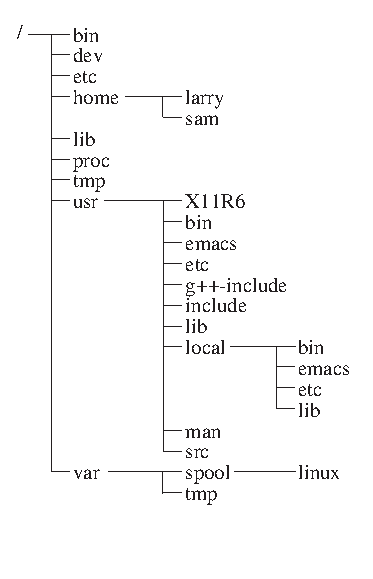
\includegraphics{tutorial/dirtree}}
\label{dirtree}
%\caption{A typical (abridged) {\linux} directory tree.}
\caption{Un t�pico �rbol de directorio {\linux} (resumido).}
\end{figure} } \fi % Kill dirtree if ASCII.

\subsection{Directorio de trabajo actual}
\index{directorio!de trabajo actual!definici�n}
\index{directorio de trabajo!definici�n}
En cualquier momento, se asume que los �rdenes que introduce se refieren a su {\bf directorio de trabajo actual}. Puede entender directorio de trabajo como el directorio en el que ''se encuentra'' 
en ese momento. Cuando accede por primera vez al sistema, su directorio de trabajo se configura como su directorio de usuario ---{\tt /home/larry}, en nuestro caso. Cuando haga referencia a un fichero,
puede referirse a �l en relaci�n a su directorio de trabajo actual, en vez de especificar el nombre de la ruta completa del fichero.

Aqu� tenemos un ejemplo. Larry tiene el directorio {\tt papers}, y {\tt papers} contiene el fichero {\tt history-final}. Si Larry quiere ver el contenido de este fichero, puede usar la orden

\begin{tscreen}
/home/larry\# more /home/larry/papers/history-final
\end{tscreen}

La orden {\tt more} simplemente muestra por pantalla un fichero, pantalla a pantalla. Como el directorio de trabajo actual de Larry es {\tt /home/larry}, se puede referir al fichero {\em en relaci�n\/} con su localizaci�n actual usando la orden

\begin{tscreen}
/home/larry\# more papers/history-final
\end{tscreen}

\index{ruta!relativa}
Si comienza el nombre del fichero (como {\tt papers/final}) con un car�cter diferente de {\tt /}, se est� refiriendo al fichero en t�rminos relativos a su directorio de trabajo actual. Esto se conoce como {\bf nombre de ruta relativo}.

\index{ruta!completa}
\index{ruta!absoluta}
Por otra parte, si comienza el nombre del fichero con una {\tt /}, el sistema lo interpreta como el nombre de la ruta absoluta ---es decir, un nombre de ruta que incluye la ruta completa hasta el fichero, comenzando en el directorio ra�z, {\tt /}. Esto se conoce como {\bf nombre de ruta absoluta}.

\subsection{Refiri�ndose al directorio inicial}
\index{directorio!inicial!\~ para referirse a@{\tt \~{}} para referise a}
\index{\~@{\tt \~{}}!para referirse al directorio inicial}
\index{home}
\index{directorio inicial}
\index{tilde}
\index{virgulilla}
Bajo {\tt tcsh} y {\tt bash}\footnote {{\tt tcsh} y {\tt bash} son dos {\em int�rprete de �rdeness} que funcionan bajo {\linux}. 
El int�rprete de �rdenes es un programa que lee los �rdenes del usuario y los ejecuta; la mayor�a de los sistema {\linux} habilitan 
{\tt tcsh} o {\tt bash} para las cuentas de los nuevos usuarios.}
puede especificar su directorio de usuario con el car�cter de la virgulilla\NT{tilde en ingl�s} ({\tt \~{}}). Por ejemplo, la orden

\begin{tscreen}
/home/larry\# more \~{}/papers/history-final
\end{tscreen}

es equivalente a

\begin{tscreen}
/home/larry\# more /home/larry/papers/history-final
\end{tscreen}

El int�rprete de �rdenes reemplaza el car�cter {\tt \~{}} por el nombre de su directorio de trabajo. 

Puede especificar tambi�n los directorios de usuario de otros usuarios con el car�cter virgulilla. La ruta {\tt \~{}karl/letters} es expandido
a {\tt /home/karl/letters} por el int�rprete de �rdenes (si {\tt /home/karl} es el directorio de usuario de Karl). El uso de la virgulilla es simplemente un atajo; no existe ning�n directorio llamado {\tt \~{}}---es s�lo una ayuda proporcionada por el int�rprete de �rdenes.

\index{{\linux}!conceptos b�sicos|)}

% Linux Installation and Getting Started    -*- TeX -*-
% basic.tex
% Copyright (c) 1992, 1993 by Matt Welsh, Larry Greenfield and Karl Fogel
%
% This file is freely redistributable, but you must preserve this copyright 
% notice on all copies, and it must be distributed only as part of "Linux 
% Installation and Getting Started". This file's use is covered by
% the copyright for the entire document, in the file "copyright.tex".
%
% Copyright (c) 1998 by Specialized Systems Consultants Inc. 
% <ligs@ssc.com>
%Revision 1 realizada el 9 de julio de 2002 por Fco. Javier Fernandez <serrador@arrakis.es>
%Revisi�n 2 Realizada el 17 de julio 2002 por Francisco Javier Fern�ndez <serrador@arrakis.es>

%\section{First steps into Linux.}
\section{Primeros Pasos en {\linux}}
\markboth{Tutorial {\linux }}{Primeros pasos en {\linux}}
Antes de que empecemos, es importante saber que todos 
los nombres de ficheros y �rdenes en un sistema {\linux} 
son {\bf case-sensitive} (que diferencian entre 
may�sculas y min�sculas a diferencia de sistemas 
operativos como MS-DOS). Por ejemplo, la orden {\tt make} 
es muy diferente de {\tt Make} o {\tt MAKE}. Lo mismo se 
cumple para nombres de ficheros y directorios.


\subsection{Movi�ndonos por la estructura de directorios.}
%\subsection{Moving around.}
Ahora que puede entrar en el sistema y que sabe c�mo referenciar los ficheros usando las rutas de los mismos, �c�mo puede cambiar el directorio de trabajo actual, para hacer la vida m�s f�cil?

\index{directorio!estructura!movi�ndose por ella con cd@movi�ndose por ella con cd {\tt cd}}
\index{cd@{\tt cd}|(}
La orden para moverse por la estructura de directorios es {\tt cd}, que es una abreviatura de ''cambiar directorio''.
Muchas de las �rdenes m�s usadas en {\linux} son de dos o tres letras.
La forma de usar la orden {\tt cd} es

\begin{tscreen}
cd \cparam{directorio}
\end{tscreen}

donde  \textsl{directorio} es el nombre del directorio que quiere que se convierta en el directorio de trabajo actual. 

Como se mencion� antes, cuando entra en el sistema, comienza en su directorio de usuario. Si Larry quisiera cambiar al subdirectorio {\tt papers}, usar�a la orden

\begin{tscreen}
/home/larry\# cd papers \\
/home/larry/papers\#
\end{tscreen}

Como puede ver, el indicador de Larry cambia para reflejar 
su directorio de trabajo actual (de forma que sabe d�nde 
se encuentra). Ahora que est� en el directorio  {\tt papers}, 
puede ver history-final con la orden

\begin{tscreen}
/home/larry/papers\# more history-final
\end{tscreen}

\index{directorio!padre!.. para referirse al@{\tt ..} para referirse al}
\index{directorio!. para referirse al@{\tt .} para referirse al}
\index{directorio padre!.. para referirse a@{\tt ..} para referirse a}

Ahora, Larry est� atascado en el subdirectorio {\tt papers}. Para regresar al directorio superior (o padre), ejecute la orden 

\begin{tscreen}
/home/larry/papers\# cd \ .. \\
/home/larry\#
\end{tscreen}

(Observe los espacios entre ``{\tt cd}'' y ``{\tt ..}''.)
Cada directorio tiene una entrada llamada ``{\tt ..}'' que se refiere al directorio padre. De forma similar, cada directorio tiene una entrada llamada ``{\tt .}''que se refiere a s� mismo. Por tanto, la orden 

\begin{tscreen}
/home/larry/papers\# cd \ .
\end{tscreen}

no lleva a ninguna parte. 

Con la orden {\tt cd} se pueden usar tambi�n rutas absolutas.
Para  cambiar  al directorio de usuario de Karl, se puede usar la orden

\begin{tscreen}
/home/larry/papers\# cd /home/karl \\
/home/karl\#
\end{tscreen}

Adem�s, la orden {\tt cd} sin argumentos le llevar� a su propio directorio de usuario. 

\begin{tscreen}
/home/karl\# cd \\
/home/larry\#
\end{tscreen}

\index{cd@{\tt cd}|)}
%\subsection{Looking at the contents of directories.}
\subsection{Mirando el contenido de los directorios}
\label{sec-ls}
\index{directorio!listar los contenidos de|(}
\index{ls@{\tt ls}|(}
\index{listando los contenidos de(}
\index{ficheros!listado|(}

Ahora que sabe c�mo moverse por los directorios, podr�a pensar, �y qu�?. Dar vueltas por los directorios no tiene mucho sentido por s� mismo, as� que introduzcamos una orden nueva,
 {\tt ls}. La orden {\tt ls} muestra un listado de ficheros y directorios, por omisi�n del directorio actual. Por ejemplo:

\begin{tscreen}
/home/larry\# ls \\
Mail \\
letters \\
papers \\
/home/larry\#
\end{tscreen}

Aqu� podemos darnos cuenta de que Larry tiene tres entradas en su directorio actual:  {\tt Mail}, {\tt letters}, y {\tt papers}. Esto no nos dice mucho -- ?` qu� son, directorios o ficheros? 
Podemos usar la opci�n {\tt -F} de la orden {\tt ls} para obtener informaci�n m�s detallada.

\begin{tscreen}
/home/larry\# ls\ --F \\
Mail/ \\
letters/ \\
papers/ \\
/home/larry\#
\end{tscreen}


Por la {\tt /} que aparece en cada nombre, sabemos que estas tres entradas son, de hecho, subdirectorios.

\index{ejecutable!definici�n}
\index{fichero!ejecutable!definici�n}

Ejecutando {\tt ls -F} puede tambi�n aparecer un ``{\tt *}'' al final de un nombre en la lista resultante, lo que indicar�a que el fichero es un {\bf ejecutable} o un programa que puede ejecutarse. 
Si no aparece nada al final de un nombre al usar {\tt ls -F}, el fichero es un ``plain old file'', es decir, no es ni un directorio ni un ejecutable.  

En general, cada orden UNIX puede tomar un cierto n�mero de opciones adem�s de otros argumentos. Estas opciones normalmente comienzan con un ``{\tt -}'', como se vi� arriba con la opci�n {\tt -F}.
 La opci�n {\tt -F} le dice a  {\tt ls} que d� m�s informaci�n acerca del tipo de ficheros involucrados --en nuestro caso, imprimiendo una {\tt /} despu�s de cada nombre de directorio. 

Si le da a {\tt ls} el nombre de un directorio, el sistema listar� los contenidos de ese directorio. 

\begin{tscreen}
/home/larry\# ls\ --F papers \\
english-lit \\
history-final \\
masters-thesis \\
notes/ \\
/home/larry\#
\end{tscreen}

O, para un listado m�s interesante, veamos qu� hay en el directorio de sistema {\tt /etc}. 

\begin{tscreen}
/home/larry\# ls /etc 
\begin{verbatim}
Images          ftpusers        lpc             rc.new          shells
adm             getty           magic           rc0.d           startcons
bcheckrc        gettydefs       motd            rc1.d           swapoff
brc             group           mount           rc2.d           swapon
brc~            inet            mtab            rc3.d           syslog.conf
csh.cshrc       init            mtools          rc4.d           syslog.pid
csh.login       init.d          pac             rc5.d           syslogd.reload
default         initrunlvl      passwd          rmt             termcap
disktab         inittab         printcap        rpc             umount
fdprm           inittab.old     profile         rpcinfo         update
fstab           issue           psdatabase      securetty       utmp
ftpaccess       lilo            rc              services        wtmp
/home/larry#
\end{verbatim}\end{tscreen}

Si es un usuario de MS-DOS, puede que se d� cuenta de que los nombres de ficheros pueden ser mayores de 8 caracteres, y pueden contener puntos en cualquier posici�n. 
Puede incluso usar m�s de un punto en un nombre de fichero.

Vayamos a la parte superior del �rbol de directorios, y luego bajemos a otro directorio con las �rdenes

\begin{tscreen}
/home/larry\# cd .. \\
/home\# cd .. \\
/\# cd usr \\
/usr\# cd bin \\
/usr/bin\#
\end{tscreen}

Puede tambi�n moverse a los directorio en un s�lo paso, haciendo {\tt cd /usr/bin}.

Pruebe a moverse por varios directorios, usando {\tt ls} y {\tt cd}. 
En algunos casos, puede que le aparezca el mensaje de error ``{\tt Permission denied}''\NT{Permiso denegado}. Esto es debido simplemente ``al sistema de seguridad UNIX'':
para poder usar las �rdenes {\tt ls} o {\tt cd}, debe tener permisos para hacerlo. Hablaremos m�s acerca de esto en
 \index{directorio!listado de los contenidos de|)}
 \index{ls@{\tt ls}|)}
 \index{listando los contenidos del directorio|)}
 \index{ficheros!listado|)}
la pagina~\pageref{sec-file-perms}.

%\subsection{Creating new directories.}
\subsection{Creaci�n de directorios nuevos}

\index{directorio!creaci�n}
\index{mkdir@{\tt mkdir}}
Es hora de aprender c�mo crear directorios. Esto requiere el uso de la orden {\tt mkdir}. Pruebe lo siguiente:

\begin{tscreen}
/home/larry\# mkdir foo \\
/home/larry\# ls -F \\
Mail/ \\
foo/ \\
letters/ \\
papers/ \\
/home/larry\# cd foo \\
/home/larry/foo\# ls \\
/home/larry/foo\# 
\end{tscreen}

!`Felicidades! Ha creado un nuevo directorio y se ha metido en �l. Como no hay 
ficheros en este nuevo directorio, aprendamos c�mo copiar ficheros de un lugar a otro.

%\subsection{Copying files.}
\subsection{Copiando ficheros}

\index{ficheros!copiar}
\index{copiar ficheros}
\index{cp@{\tt cp}}

Para copiar ficheros, use el orden {\tt cp}, como se muestra aqu�:

\begin{tscreen}
/home/larry/foo\# cp /etc/termcap\ \ . \\
/home/larry/foo\# cp /etc/shells\ \ . \\
/home/larry/foo\# ls\ --F \\
shells\ \ \ \ \ termcap  \\
/home/larry/foo\# cp shells bells \\
/home/larry/foo\# ls\ --F \\
bells\ \ \ \ \ shells\ \ \ \ \ termcap \\
/home/larry/foo\# 
\end{tscreen}

La orden {\tt cp} copia los ficheros escritos en la l�nea de �rdenes al fichero o directorio dados como �ltimo argumento. D�se cuenta de que usamos``{\tt .}'' para referirnos al directorio 
actual.

%\subsection{Moving files.}
\subsection{Moviendo ficheros}
\index{fichero!mover}
\index{mover ficheros}
\index{mv@{\tt mv}}

El orden {\tt mv} mueve ficheros, en vez de copiarlos. 
La sintaxis es muy parecida:

\begin{tscreen}
/home/larry/foo\# mv termcap sells \\
/home/larry/foo\# ls -F \\
bells\ \ \ \ \ sells\ \ \ \ \ shells \\
/home/larry/foo\# 
\end{tscreen}

D�se cuenta de que el fichero {\tt termcap} ha sido renombrado a {\tt shells}. Puede adem�s usar la orden {\tt mv} para mover un fichero a un directorio completamente 
nuevo.

\blackdiamond {\bf Nota:} {\tt mv} y {\tt cp} sobreescribir�n un fichero de destino que tiene el mismo nombre sin pregunt�rselo. Tenga cuidado cuando mueva un fichero a otro directorio. Puede que haya un fichero con el mismo nombre en ese directorio, !`que ser� sobreescrito!

%\subsection{Deleting ficheros and directories.}
\subsection{Borrando ficheros y directorios}
\index{fichero!borrar}
\index{borrar!ficheros}
\index{rm@{\tt rm}}
Usted tiene ahora una fea rima, que ha creado usando el orden {\tt ls}.
Para borrar un fichero, use el orden {\tt rm}, que proviene de ''remove'',\NT{quitar} como se muestra aqu�:

\begin{tscreen}
/home/larry/foo\# rm bells sells \\
/home/larry/foo\# ls -F \\
shells \\
/home/larry/foo\#
\end{tscreen}

No nos queda nada salvo shells, pero no nos quejaremos. D�se cuenta de que {\tt rm} no 
le preguntar� antes de borrar un fichero, as� que tenga cuidado.

\index{borrar!directorio}
\index{directorio!borrar}
\index{rmdir@{\tt rmdir}}
Una orden relacionada con {\tt rm} es {\tt rmdir}. Este orden borra un directorio, pero s�lo si 
el directorio est� vac�o. Si el directorio contiene alg�n fichero o 
subdirectorio, {\tt rmdir} protestar�.

%\subsection{Looking at ficheros.}
\subsection{Mirando en los ficheros}
\index{ficheros!ver el contenido de}
\index{more@{\tt more}}
\index{cat@{\tt cat}!para ver el contenido de un fichero}
Las �rdenes {\tt more} y {\tt cat} se usan para ver el contenido de los ficheros. El orden {\tt more} muestra un fichero, una pantalla completa cada vez, mientras que {\tt cat} muestra el fichero completo de una vez.

Para ver el contenido del fichero {\tt shells}, use la orden

\begin{tscreen}
/home/larry/foo\# more shells
\end{tscreen}

En caso de que est� interesado en lo que contiene {\tt shells}, es una lista de int�rpretes de �rdenes (shell) v�lidos en su sistema. En la mayor�a de los sistemas, esto incluye {\tt /bin/sh}, {\tt /bin/bash} y {\tt /bin/csh}. Hablaremos acerca de estos diferentes tipos de int�rpretes de �rdenes m�s adelante.

Mientras est� usando {\tt more}, presione \key{Space} para ver la siguiente p�gina de texto, y \key{b} para ver la p�gina anterior. Hay otras �rdenes disponibles en {\tt more},
�stos son s�lo los b�sicos. Podr� salir de {\tt more} pulsando \key{q}.

Salga de {\tt more} y pruebe {\tt cat /etc/termcap}. Probablemente el texto ir� demasiado r�pido para que pueda leerlo. 
El nombre ``{\tt cat}'' proviene de hecho de ``concatenate'', que es el verdadero uso del programa. El orden {\tt cat} puede usarse para "encadenar" los contenidos de varios ficheros y guardar el
 resultado en otro fichero.
Volveremos a esto en la secci�n ~\ref{sec-shell-script}.

%\subsection{Getting online help.}
\subsection{Obteniendo ayuda en l�nea}


\index{{\linux}!p�ginas de manual para}
\index{ayuda!en l�nea}
\index{p�ginas del manual}
\index{maunal de linux}
Casi todos los sistemas UNIX, incluyendo {\linux}, facilitan lo que se conoce como {\bf p�ginas del manual}. Estas p�ginas contienen documentaci�n acerca de �rdenes del sistema, recursos, ficheros
 de configuraci�n, etc.

\index{man@{\tt man}}

La orden usada para acceder a las p�ginas del manual es {\tt man}. Si est� interesado en aprender nuevas opciones de la orden {\tt ls} puede escribir

\begin{tscreen}
/home/larry\# man ls
\end{tscreen}

y se mostrar� la p�gina del manual para {\tt ls}.

Por desgracia, la mayor�a de las p�ginas de manual est�n escritas por personas que ya tienen alguna idea de lo que la orden o recurso hace. Por esta raz�n, las p�ginas del manual, a menudo,
 contienen s�lo los detalles t�cnicos de la orden, sin mucha explicaci�n. De todos modos, las p�ginas del manual pueden constituir un recurso muy valioso para refrescar su memoria si se le 
olvida la sintaxis de una orden. Las p�ginas del manual le hablar�n adem�s de �rdenes que no veremos en este libro.

Sugiero que pruebe {\tt man} para las �rdenes que ya hemos visto y cuando
veamos alguno nuevo. Algunas de estas �rdenes no tendr�n p�gina de manual,
por distintas razones. Primero, las p�ginas de manual puede que no se hayan
escrito todav�a. El proyecto de documentaci�n de {\linux} tambi�n es responsable de
las p�ginas de manual de {\linux}. Estamos acumulando poco a poco la
mayor�a de las p�ginas de manual disponibles para el sistema). Segundo, la
orden podr�a ser una orden interna del shell, o un alias (que se
discutir� en la p�gina ~\pageref{sec-shells-cmds}), la cual podr�a no tener
una p�gina de manual propia. Un ejemplo es {\tt cd}, que es una orden
interna del shell. El shell por s� s�lo procesa la orden {\tt cd} --- 
no hay un programa separado que implemente esta orden.

% {\linux} Installation and Getting Started    -*- TeX -*-
% msdos.tex
% Copyright (c) 1992, 1993 by Matt Welsh <mdw@sunsite.unc.edu>
%
% This file is freely redistributable, but you must preserve this copyright 
% notice on all copies, and it must be distributed only as part of "{\linux} 
% Installation and Getting Started". This file's use is covered by the 
% copyright for the entire document, in the file "copyright.tex".
%
% Copyright (c) 1998 by Specialized Systems Consultants Inc. 
% <ligs@ssc.com>

%\section{Accessing MS-DOS files.}
\section{Acceder a los ficheros MS-DOS\TM}
\markboth{Caracter�sticas Avanzadas}{Acceso a ficheros MS-DOS\tm}
\label{sec-msdos-mount}
\index{MS-DOS!acceder ficheros desde}
\index{ficheros!MS-DOS}
Si, por cualquier retorcida y extrafalaria raz�n, quiere acceder a ficheros
de MS-DOS, lo  podr� hacer f�cilmente desde {\linux}.

\index{MS-DOS!montando una partici�n bajo {\linux}}
\index{mount@{\tt mount}!para montar una partici�n MS-DOS}
La manera normal de acceder a los ficheros de MS-DOS es montar una partici�n MS-DOS o
un disco flexible bajo {\linux}, lo cual permite acceder a los ficheros directamente a trav�s
del sistema de ficheros. Por ejemplo, si tiene un disco flexible MS-DOS en
{\tt /dev/fd0}, la orden

\begin{tscreen}
\# mount -t msdos /dev/fd0 /mnt
\end{tscreen}

lo montar� en {\tt /mnt}. Consulte la Secci�n~\ref{sec-floppy} para m�s
informaci�n sobre c�mo montar discos flexibles.

Tambi�n puede montar una partici�n MS-DOS de su disco duro para que sea
accesible desde {\linux}. Si tiene una partici�n MS-DOS en {\tt /dev/hda1}, la orden

\begin{tscreen}
\# mount -t msdos /dev/hda1 /mnt
\end{tscreen}

la monta. Aseg�rese de desmontar ({\tt umount}) la partici�n cuando haya terminado
de usarla. Tambi�n se puede hacer que una partici�n MS-DOS se monte autom�ticamente
en el momento del arranque si incluye la entrada en {\tt /etc/fstab}. Consulte la
Secci�n~\ref{sec-manage-fs} para m�s detalles. La siguiente l�nea en {\tt
/etc/fstab} monta una partici�n MS-DOS en {\tt /dev/hda1} en el
directorio {\tt /dos}.

\begin{tscreen}
/dev/hda1\ \ \ \ \ /dos\ \ \ \ \ msdos \ \ \ \ \ defaults
\end{tscreen}

Tambi�n puede montar los sistemas de ficheros VFAT usados por Windows 95 y 98:

\begin{tscreen}
\# mount -t vfat /dev/hda1 /mnt
\end{tscreen}

Esto permite acceder a los nombres largos de ficheros de Windows 95\tm. Esto s�lo
se aplica a particiones que realmente tengan almacenados los nombres en formato
largo. No se puede montar un sistema de ficheros FAT16 normal y usarlo para
obtener nombres de ficheros largos.

\index{MS-DOS!uso de Mtools para acceder a ficheros}
El software Mtools tambi�n puede ser usado para acceder a ficheros MS-DOS\tm. Las
�rdenes {\tt mcd}, {\tt mdir}, y {\tt mcopy} se comportan todas como sus
equivalentes MS-DOS\tm. Si instala las Mtools, deber�a tener p�ginas del manual
disponibles para estas �rdenes.

\index{MS-DOS!ejecuci�n de programas bajo {\linux}}
\index{MS-DOS!emulador}
\index{Microsoft Windows!emulador} 
Acceder a ficheros MS-DOS es una cosa; ejecutar programas MS-DOS es
otra. Hay un emulador de MS-DOS\tm en desarrollo para {\linux}; es
f�cil de conseguir, y est� inclu�do en la mayor�a de las distribuciones.
Tambi�n se puede conseguir en muchos sitios, incluyendo los sitios
FTP para {\linux} listados en el Ap�ndice~\ref{app-ftp}. El emulador de MS-DOS est�
considerado como lo suficientemente potente para hacer funcionar un buen n�mero de
aplicaciones, incluyendo Wordperfect\tm, desde {\linux}. Sin embargo, {\linux} y MS-DOS son
sistemas operativos marcadamente diferentes. La potencia de cualquier emulador de MS-DOS
bajo UNIX est� limitada. Adem�s, est� en desarrollo un emulador de Microsoft Windows
que corra bajo X Window.











% \linux Installation and Getting Started    -*- TeX -*-
% commands.tex
% Copyright (c) 1992, 1993 by Matt Welsh, Larry Greenfield and Karl Fogel
%
% This fichero is freely redistributable, but you must preserve this copyright 
% notice on all copies, and it must be distributed only as part of "\linux 
% Installation and Getting Started". This fichero's use is covered by
% the copyright for the entire document, in the fichero "copyright.tex".
%
% Copyright (c) 1998 by Specialized Systems Consultants Inc. 
% <ligs@ssc.com>
% Revisi�n 1 por Fco. Javer Fern�ndez <serrador@arrakis.es> 9 de julio del 2002
%
%\section{Summary of basic UNIX commands.}\label{sec-command-summ}
\section{Sumario de �rdenes b�sicas}
\label{sec-command-summ}
\markboth{Tutorial de {\linux}}{Sumario de �rdenes b�sicas UNIX}

\index{�rdenes!sumario de b�sicas|(}
Esta secci�n introduce algunas de las m�s �tiles �rdenes b�sicas de un sistema UNIX, incluyendo aqu�llas que son cubiertas en la secci�n anterior.

\index{�rdenes!-@{\tt -} flag de opci�n de orden}
\index{flag@{\tt -} de opci�n de orden}
F�jese en que las opciones suelen empezar con ``{\tt -}'', y en la mayor�a de los casos es posible especificar m�s de una opci�n con un �nico ``{\tt -}''. Por ejemplo, en vez de usar {\tt ls -l -F}, 
se puede escribir {\tt ls -lF}.

En lugar de dar una lista de cada una de las opciones de una orden, ahora s�lo vamos a presentar �rdenes �tiles o importantes. De hecho, la mayor�a de estas �rdenes tienen muchas opciones 
que nunca usar�. Puede usar {\tt man} para echar un vistazo a las p�ginas de manual de cada orden, el cu�l lista todas las opciones disponibles.

D�se cuenta tambi�n de que muchas de estas �rdenes toman como argumento una lista de ficheros o directorios, indicados en esta tabla por ``\textsl{fichero1} \ldots \textsl{ficheroN}''. Por ejemplo,
la orden {\tt cp} toma como argumentos una lista de ficheros para copiar, seguido del fichero o directorio destino. Cuando va a copiar m�s de un fichero, el destino debe ser un directorio.

\begin{dispitems}

\index{cd@{\tt cd}}
\ditem {{\tt cd}}
Cambia el directorio de trabajo actual \\
Sintaxis: {\tt cd \cparam{directorio}} \\
Donde \textsl{directorio} es el directorio al que se quiere cambiar. ``{\tt .}''
hace referencia al directorio actual, ``{\tt ..}'' al directorio padre. Si no se especifica ning�n directorio le lleva, por omisi�n, a su directorio de usuario. \\

Ejemplo: {\tt cd ../foo} sube el directorio actual un nivel, y entonces, se introduce en el directorio {\tt foo}.

\index{ls@{\tt ls}}
\ditem {{\tt ls}}
Muestra informaci�n acerca de los ficheros y directorios nombrados. \\
Sintaxis: {\tt ls \cparam{ficheros} }\\
Donde \textsl{ficheros} consiste en los nombres de ficheros o directorios que se quieren listar. Las opciones que m�s se usan son {\tt -F} (para mostrar el tipo de fichero) y {\tt -l}
 (para mostrar una lista ''ampliada'' incluyendo el tama�o de los ficheros, propietario, permisos, etc.). \\
Ejemplo: {\tt ls -lF /home/larry} muestra los contenidos del directorio {\tt /home/larry}.

\index{cp@{\tt cp}}
\ditem {{\tt cp}} 
Copia uno o m�s ficheros a otro fichero o directorio. \\
Sintaxis: {\tt cp \cparam{ficheros}
\cparam{destino}} \\
Donde \textsl{ficheros} indica los ficheros que hay que copiar, y
\textsl{destino} es el fichero o directorio destino. \\

Ejemplo: {\tt cp ../frog joe} copia el fichero {\tt ../frog} al fichero o directorio {\tt joe}.

\index{mv@{\tt mv}}
\ditem {{\tt mv}} 
Mueve uno o m�s ficheros a otro directorio. Esta orden hace el equivalente de una copia seguido del borrado del fichero original.
Puede usar esto para renombrar ficheros, como con la orden de MS-DOS {\tt RENAME}. \\
Sintaxis: {\tt mv \cparam{ficheros}
\cparam{destino}} \\
Donde \textsl{ficheros} indica los arhivos que hay que mover, y
\textsl{destino} es el fichero o directorio destino. \\

Ejemplo: {\tt mv ../frog joe} mueve el fichero {\tt ../frog} al fichero o directorio {\tt joe}.

\index{rm@{\tt rm}}
\ditem {{\tt rm}} 
Borra ficheros. F�jese en que cuando borra un fichero bajo UNIX, 
son irrecuperables (al contrario que con MS-DOS, donde normalmente se puede ''desborrar'' el fichero). \\
Sintaxis: {\tt rm \cparam{ficheros}} \\
Donde \textsl{ficheros} describe el nombre de los ficheros que hay que borrar. \\
La opci�n {\tt -i} le pide confirmaci�n antes de borrar el fichero. \\

Ejemplo: {\tt rm -i /home/larry/joe /home/larry/frog} borra los ficheros {\tt joe} y {\tt frog} en {\tt /home/larry}.


\index{mkdir@{\tt mkdir}}
\ditem {{\tt mkdir}}
Crea nuevos directorios.\\
Sintaxis: {\tt mkdir \cparam{dirs} }\\
Donde \textsl{dirs} son los directorios que hay que crear. \\

Ejemplo: {\tt mkdir /home/larry/test} crea el directorio {\tt test}
en {\tt /home/larry}.

\index{rmdir@{\tt rmdir}}
\ditem {{\tt rmdir}} 
Borra directorios vac�os. Cuando use {\tt rmdir}, el directorio de trabajo actual no debe estar dentro del directorio que se pretende borrar. \\
Sintaxis: {\tt rmdir \cparam{dirs} }\\
Donde \textsl{dirs} define los directorios que hay que borrar. \\

Ejemplo: {\tt rmdir /home/larry/papers} borra el directorio {\tt /home/larry/papers}, si est� vac�o. 

\index{man@{\tt man}}
\ditem {{\tt man}} 
Muestra la p�gina de manual para la orden o recurso dado (es decir, no una utilidad del sistema que no sea 
una orden, como una funci�n de biblioteca.)\\

Sintaxis: {\tt man \cparam{command}} \\

Donde \textsl{command} es el nombre de la orden o recurso del que se quiere conseguir ayuda.\\

Ejemplo: {\tt man ls} le da informaci�n acerca de la orden {\tt ls}.

\index{more@{\tt more}}
\ditem {{\tt more}} 
Muestra informaci�n del contenido de los ficheros nombrados, pantalla por pantalla. \\
Sintaxis: {\tt more \cparam{ficheros}} \\
Donde \textsl{ficheros} indica los ficheros que se quieren mostrar. \\

Ejemplo: {\tt more papers/history-final} muestra el fichero {\tt papers/history-final}.

\index{cat@{\tt cat}}
\ditem {{\tt cat}} 
Oficialmente usado para concatenar ficheros, {\tt cat} tambi�n se usa para mostrar los contenidos de un fichero por pantalla. \\
Sintaxis: {\tt cat \cparam{ficheros}} \\
Donde \textsl{ficheros} indica los ficheros que se quieren mostrar. \\

Ejemplo: {\tt cat letters/from-mdw} muestra el fichero {\tt letters/from-mdw}.

\index{echo@{\tt echo}}
\ditem{{\tt echo}}
Muestra en la pantalla los argumentos que se le pasan a la orden. \\
Sintaxis: {\tt echo \cparam{args}} \\
Donde \textsl{args} indica los argumentos que se quieren mostrar. \\

Ejemplo: {\tt echo ``Hello world''} muestra la cadena ``{\tt Hello world}''.

\index{grep@{\tt grep}}
\ditem{{\tt grep}}
Muestra cada l�nea en uno o m�s ficheros que contiene un patr�n dado. \\
Sintaxis: {\tt grep \cparam{pattern} \cparam{ficheros}} \\
Donde \textsl{pattern} es un patr�n, y 
\textsl{ficheros} indica los ficheros donde se quiere buscar dicho patr�n. \\

Ejemplo: {\tt grep loomer /etc/hosts} muestra cada l�nea en el fichero {\tt /etc/hosts} que contiene el patr�n ``{\tt loomer}''.

\end{dispitems}

\index{�rdenes!sumario de las b�sicas|)}




\chapter{El sistema de archivos}
\label{filesystem-chapter}

\ChapterDescription{Este capitulo describe c�mo el kernel de Linux
  gestiona los ficheros en los sistemas de ficheros soportados por
  �ste.  Describe el Sistema de Ficheros Virtual (VFS) y explica c�mo
  los sistemas de ficheros reales del kernel de Linux son soportados.}

\index{File system} Una de los rasgos m�s importantes de Linux es su
soporte para diferentes sistemas de ficheros.  �sto lo hace muy
flexible y bien capacitado para coexistir con muchos otros sistemas
operativos.  En el momento de escribir �sto, Linux soporta 15 sistemas
de ficheros; \texttt{ext}, \texttt{ext2}, \texttt{xia},
\texttt{minix}, \texttt{umsdos}, \texttt{msdos}, \texttt{vfat},
\texttt{proc}, \texttt{smb}, \texttt{ncp}, \texttt{iso9660},
\texttt{sysv}, \texttt{hpfs}, \texttt{affs} and \texttt{ufs}, y sin
duda, con el tiempo se a�adir�n m�s.

En Linux, como en Unix\tm, a los distintos sistemas de ficheros que el
sistema puede usar no se accede por identificadores de dispositivo
(como un n�mero o nombre de unidad) pero, en cambio se combinan en una
simple structura jer�rquica de �rbol que representa el sistema de
ficheros como una entidad �nica y sencilla.  Linux a�ade cada sistema
de ficheros nuevo en este simple �rbol de sistemas de ficheros cuando
se monta.  Todos los sistemas de ficheros, de cualquier tipo, se
montan sobre un directorio y los ficheros del sistema de ficheros son
el contenido de ese directorio.  Este directorio se conoce como
directorio de montaje o punto de montaje.  Cuando el sistema de
ficheros se desmonta, los ficheros propios del directorio de montaje
son visibles de nuevo.

Cuando se inicializan los discos (usando \eg{fdisk}, por ejemplo)
tienen una estructura de partici�n inpuesta que divide el disco f�sico
en un n�mero de particiones l�gicas.  Cada partici�n puede mantener un
sistema de ficheros, por ejemplo un sistema de ficheros \texttt{EXT2}.
Los sistemas de ficheros organizan los ficheros en structuras
jer�rquicas l�gicas con directorios, enlaces flexibles y m�s
contenidos en los bloques de los dispositivos f�sicos.  Los
dispositivos que pueden contener sistemas de ficheros se conocen con
el nombre de dispositivos de bloque.  La partici�n de disco IDE
\fn{/dev/hda1}, la primera partici�n de la primera unidad de disco en
el sistema, es un dispositivo de bloque.  Los sistemas de ficheros de
Linux contemplan estos dispositivos de bloque como simples colecciones
lineales de bloques, ellos no saben o tienen en cuenta la geometr�a
del disco f�sico que hay debajo.  Es la tarea de cada controlador de
dispositivo de bloque asignar una petici�n de leer un bloque
particular de su dispositivo en t�rminos comprensibles para su
dispositivo; la pista en cuesti�n, sector y cilindro de su disco duro
donde se guarda el bloque.  Un sistema de ficheros tiene que mirar,
sentir y operar de la misma forma sin importarle con que dispositivo
est� tratando.  Por otra parte, al usar los sistemas de ficheros de
Linux, no importa (al menos para el usuario del sistema) que estos
distintos sistemas de ficheros est�n en diferentes soportes
controlados por diferentes controladores de hardware.  El sistema de
ficheros puede incluso no estar en el sistema local, puede ser
perfectamente un disco remoto montado sobre un enlace de red.
Considerese el siguiente ejemplo donde un sistema Linux tiene su
sistema de ficheros ra�z en un disco SCSI:
\begin{verbatim}
A         E         boot      etc       lib       opt       tmp       usr
C         F         cdrom     fd        proc      root      var       sbin
D         bin       dev       home      mnt       lost+found
\end{verbatim}
Ni los usuarios ni los programas que operan con los ficheros necesitan
saber que \fn{/C} de hecho es un sistema de ficheros VFAT montado que
est� en el primer disco IDE del sistema.  En el ejemplo (que es mi
sistema Linux en casa), \fn{/E} es el disco IDE primario en la segunda
controladora IDE.  No importa que la primera controladora IDE sea una
controladora PCI y que la segunda sea una controladora ISA que tambi�n
controla el IDE CDROM.  Puedo conectarme a la red donde trabajo usando
un modem y el protocolo de red PPP y en este caso puedo remotamente
montar mis sistemas de ficheros Linux \axp\ sobre \fn{/mnt/remote}.

Los ficheros en un sistema de ficheros son grupos de datos; el fichero
que contiene las fuentes de este cap�tulo es un fichero ASCII llamado
\fn{filesystems.tex}.  Un sistema de ficheros no s�lo posee los datos
contenidos dentro de los ficheros del sistema de ficheros, adem�s
mantiene la estructura del sistema de ficheros.  Mantiene toda la
informaci�n que los usuarios de Linux y procesos ven como ficheros,
directorios, enlaces flexibles, informaci�n de protecci�n de ficheros
y as�.  Por otro lado debe mantener esa informaci�n de forma eficiente
y segura, la integridad b�sica del sistema operativo depende de su
sistema de ficheros.  Nadie usaria un sistema operativo que perdiera
datos y ficheros de forma aleatoria\footnote{Bueno, no con
  conocimiento, sin embargo me he topado con sistemas operativos con
  m�s abogados que programadores tiene Linux}.

\texttt{Minix}, el primer sistema de ficheros que Linux tuvo es
bastante restrictivo y no era muy r�pido.  \texttt{Minix}, the first
file system that Linux had is rather restrictive and lacking in
performance.\index{Minix} Sus nombres de ficheros no pueden tener m�s
de 14 caracteres (que es mejor que nombres de ficheros 8.3) y el
tama�o m�ximo de ficheros es 64 MBytes.  64 MBytes puede a primera
vista ser suficiente pero se necesitan tama�os de ficheros m�s grandes
para soportar incluso modestas bases de datos.  El primer sistema de
ficheros dise�ado especificamente para Linux, el sistema de Ficheros
Extendido, o \texttt{EXT}, fue introducido en Abril de 1992 y solvent�
muchos problemas pero era aun falto de rapidez.  \index{EXT}
\index{Extended File system} As�, en 1993, el Segundo sistema de
Ficheros Extendido, o \texttt{EXT2}, fue a�adido.  \index{EXT2}
\index{Second Extended File system} Este es el sistema de ficheros que
se describe en detalle m�s tarde en este cap�tulo.

Un importante desarrollo tuvo lugar cuando se a�adi� en sistema de
ficheros EXT en Linux.  El sistema de ficheros real se separ� del
sistema operativo y servicios del sistema a favor de un interfaz
conocido como el sistema de Ficheros Virtual, o VFS.  \index{VFS}
\index{Virtual File system} VFS permite a Linux soportar muchos,
incluso muy diferentes, sistemas de ficheros, cada uno presentando un
interfaz software com�n al VFS.  Todos los detalles del sistema de
ficheros de Linux son traducidos mediante software de forma que todo
el sistema de ficheros parece id�ntico al resto del kernel de Linux y
a los programas que se ejecutan en el sistema.  La capa del sistema de
Ficheros Virtual de Linux permite al usuario montar de forma
transparente diferentes sistemas de ficheros al mismo tiempo.

El sistema de Ficheros Virtual est� implementado de forma que el
acceso a los ficheros es r�pida y tan eficiente como es posible.
Tambi�n debe asegurar que los ficheros y los datos que contiene son
correctos.  Estos dos requisitos pueden ser incompatibles uno con el
otro.  El VFS de Linux mantiene una antememoria con informaci�n de
cada sistema de ficheros montado y en uso.  Se debe tener mucho
cuidado al actualizar correctamente el sistema de ficheros ya que los
datos contenidos en las antememorias se modifican cuando cuando se
crean, escriben y borran ficheros y directorios.  Si se pudieran ver
las estructuras de datos del sistema de ficheros dentro del kernel en
ejecuci�n, se podria ver los bloques de datos que se leen y escriben
por el sistema de ficheros.  Las estructuras de datos, que describen
los ficheros y directorios que son accedidos serian creadas y
destruidas y todo el tiempo los controladores de los dispositivo
estarian trabajando, buascando y guardando datos.  La antememoria o
cach� m�s importantes es el Buffer Cache, que est� integrado entre
cada sistema de ficheros y su dispositivo de bloque.  Tal y como se
accede a los bloques se ponen en el Buffer Cache y se almacenan en
varias colas dependiendo de sus estados.  El Buffer Cache no s�lo
mantiene buffers de datos, tambien ayuda a administrar el interfaz
as�ncrono con los controladores de dispositivos de bloque.

\section{The Second Extended File system (EXT2)}
\index{EXT2}
\begin{figure}
\begin{center}
{\centering \includegraphics{fs/ext2.eps} \par}
\end{center}
\caption{Physical Layout of the EXT2 File system}
\label{ext2fs-figure}
\end{figure}
El Segundo sistema de ficheros Extendido fue pensado (por R�my Card)
como un sistema de ficheros extensible y poderoso para Linux.  Tambi�n
es el sistema de ficheros m�s �xito tiene en la comunidad Linux y es
b�sico para todas las distribuciones actuales de Linux.
\SeeModule{fs/�ext2/�*} El sistema de ficheros EXT2, como muchos
sistemas de ficheros, se construye con la premisa de que los datos
contenidos en los ficheros se guarden en bloques de datos.  Estos
bloques de datos son todos de la misma longitud y, si bien esa
longitud puede variar entre diferentes sistemas de ficheros EXT2 el
tama�o de los bloques de un sistema de ficheros EXT2 en particular se
decide cuando se crea (usando \eg{mke2fs}).  El tama�o de cada fichero
se redondea hasta un numero entero de bloques.  Si el tama�o de bloque
es 1024 bytes, entonces un fichero de 1025 bytes ocupar� dos bloques
de 1024 bytes.  Desafortunadamente esto significa que en promedio se
desperdicia un bloque por fichero.
Normalmente en ordenadores se cambia la carga de CPU por m�s espacio de memoria o de disco utilizado. En este caso Linux, como muchos sistemas operativos, cambia una ineficiencia relativa en el uso del disco a cambio de reducir la carga de la CPU.

No todos los bloques del sistema de ficheros contienen datos, algunos
deben usarse para mantener la informaci�n que describe la estructura
del sistema de ficheros.  EXT2 define la topologia del sistema de
ficheros describiendo cada fichero del sistema con una estructura de
datos inodo.  Un inodo describe que bloques ocupan los datos de un
fichero y tambi�n los permisos de acceso del fichero, las horas de
modificaci�n del fichero y el tipo del fichero.  Cada fichero en el
sistema de ficheros EXT2 se describe por un �nico inodo y cada inodo
tiene un �nico n�mero que lo identifica.  Los inodos del sistema de
ficheros se almacenan juntos en tablas de inodos.  Los directorios
EXT2 son simplemente ficheros especiales (ellos mismos descritos por
inodos) que contienen punteros a los inodos de sus entradas de
directorio.

La figura�\ref{ext2fs-figure} muestra la disposici�n del sistema de
ficheros EXT2 ocupando una serie de bloques en un dispositivo
estructurado bloque.  Por la parte que le toca a cada sistema de
ficheros, los dispositivos de bloque son s�lo una serie de bloques que
se pueden leer y escribir.  Un sistema de ficheros no se debe
preocupar donde se debe poner un bloque en el medio f�sico, eso es
trabajo del controlador del dispositivo.  Siempre que un sistema de
ficheros necesita leer informaci�n o datos del dispositivo de bloque
que los contiene, pide que su controlador de dispositivo lea un n�mero
entero de bloques.  El sistema de ficheros EXT2 divide las particiones
l�gicas que ocupa en Grupos de Bloque (Block Groups).  \index{EXT2
  Block Groups} Cada grupo duplica informaci�n cr�tica para la
integridad del sistema de ficheros ya sea valiendose de ficheros y
directorios como de bloques de informaci�n y datos.  Esta duplicaci�n
es necesaria por si ocurriera un desastre y el sistema de ficheros
necesitara recuperarse.  Los subapartados describen con m�s detalle
los contenidos de cada Grupo de Bloque.

\subsection{El inodo de EXT2}
\begin{figure}
\begin{center}
{\centering \includegraphics{fs/ext2_inode.eps} \par}
\end{center}
\caption{El inodo de EXT2}
\label{ext2fs-inode-figure}
\end{figure}
\index{El inodo de EXT2} \index{Estructuras de datos, el inodo EXT2} En el sistema de ficheros \texttt{EXT2}, el inodo es el bloque de construcci�n
b�sico; cada fichero y directorio del sistema de ficheros es descrito
por un y s�lo un inodo.  Los inodos EXT2 para cada Grupo de Bloque se
almacenan juntos en la table de inodos con un mapa de bits que permite
al sistema seguir la pista de inodos reservados y libres.  La
figura�\ref{ext2fs-inode-figure} muestra el formato de un inodo EXT2,
entre otra informaci�n, contiene los siguientes campos:
\SeeModule{include/\-linux/\-ext2\_fs\_i.h}
\begin{description}
\item [mode] Esto mantiene dos partes de informaci�n; qu� inodo
  describe y los permisos que tienen los usuarios.  Para EXT2, un
  inodo puede describir un ficheros, directorio, enlace simb�lico,
  dispositivo de bloque, dispositivo de caracter o FIFO.
\item [Owner Information] Los identificadores de usuario y grupo de
  los due�os de este fichero o directorio.  Esto permite al sistema de
  ficheros aplicar correctamente el tipo de acceso,
\item [Size] El tama�o en del fichero en bytes,
\item [Timestamps] La hora en la que el inodo fue creado y la �ltima
  hora en que se modific�,
\item [Datablocks] Punteros a los bloques que contienen los datos que
  este inodo describe.  Los doce primeros son punteros a los bloques
  f�sicos que contienen los datos descritos por este inodo y los tres
  �ltimos punteros contienen m�s y m�s niveles de indirecci�n.  Por
  ejemplo, el puntero de doble indirecci�n apunta a un bloque de
  punteros que apuntan a bloques de punteros que apuntan a bloques de
  datos.  Esto significa que ficheros menores o iguales a doce bloques
  de datos en longitud son m�s facilmente accedidos que ficheros m�s
  grandes.
\end{description}
Indicar que los inodos EXT2 pueden describir ficheros de dispositivo
especiales.  No son ficheros reales pero permiten que los programas
puedan usarlos para acceder a los dispositivos.  Todos los ficheros de
dispositivo de \fn{/dev} est�n ahi para permitir a los programas
acceder a los dispositivos de Linux.  Por ejemplo el programa
\eg{mount} toma como argumento el fichero de dispositivo que el
usuario desee montar.

\subsection{El superbloque EXT2}
\index{Superbloque EXT2} El Superbloque contiene una descripci�n del
tama�o y forma base del sistema de ficheros.  La informaci�n contenida
permite al administrador del sistema de ficheros usar y mantener el
sistema de ficheros.  Normalmente s�lo se lee el Superbloque del Grupo
de Bloque 0 cuando se monta el sistema de ficheros pero cada Grupo de
Bloque contiene una copia duplicada en caso de que se corrompa sistema
de ficheros.  Entre otra informaci�n contiene el:
\SeeModule{include/\-linux/\-ext2\_fs\_sb.h}
\begin{description}
\item [Magic Number] Esto permite al software de montaje comprobar que
  es realmente el Superbloque para un sistema de ficheros EXT2.  Para
  la versi�n actual de \texttt{EXT2} �ste es \hex{EF53}.
\item [Revision Level] Los niveles de revisi�n mayor y menor permiten
  al c�digo de montaje determinar si este sistema de ficheros soporta
  o no caracter�sticas que s�lo son disponibles para revisiones
  particulares del sistema de ficheros.  Tambi�n hay campos de
  compatibilidad que ayudan al c�digo de montaje determinar que nuevas
  caracter�sticas se pueden usar con seguridad en ese sistema de
  ficheros,
\item [Mount Count and Maximum Mount Count] Juntos permiten al sistema
  determinar si el sistema de ficheros fue comprobado correctamente.
  El contador de montaje se incrementa cada vez que se monta el
  sistema de ficheros y cuando es igual al contador m�ximo de montaje
  muestra el mensaje de aviso �maximal mount count reached, running
  e2fsck is recommended�,
\item [Block Group Number] El n�mero del Grupo de Bloque que tiene la
  copia de este Superbloque,
\item [Block Size] El tama�{o} de bloque para este sistema deficheros
  en bytes, por ejemplo 1024 bytes,
\item [Blocks per Group] El n�mero de bloques en un grupo.  Como el
  tama�o de bloque �ste se fija cuando se crea el sitema de ficheros,
\item [Free Blocks] EL n�mero de bloques libres en el sistema de
  ficheros,
\item [Free Inodes] El n�mero de Inodos libres en el sistema de
  ficheros,
\item [First Inode] Este es el n�mero de inodo del primer inodo en el
  sistema de ficheros.  El primer inodo en un sistema de ficheros EXT2
  ra�z seria la entrada directorio para el directorio '/'.
\end{description}

\subsection{The EXT2 Group Descriptor}
\index{EXT2 Group Descriptor} Cada Grupo de Bloque tiene una
estructura de datos que lo describe.  Como el Superbloque, todos los
descriptores de grupo para todos los Grupos de Bloque se duplican en
cada Grupo de Bloque en caso de corrupci�n del sistema de fichero.
\SeeCode{ext2\_group\_desc}{include/\-linux/\-ext2\_fs.h} Cada
Descriptor de Grupo contiene la siguiente informaci�n:
\begin{description}
\item [Blocks Bitmap] El n�mero de bloque del mapa de bits de bloques
  reservados para este Grupo de Bloque.  Se usa durante la reseva y
  liberaci�n de bloques,
\item [Inode Bitmap] El n�mero de bloque del mapa de bits de inodos
  reservados para este Grupo de Bloques.  Se usa durante la reserva y
  liberaci�n de inodos,
\item [Inode Table] El n�mero de bloque del bloque inicial para la
  tabla de inodos de este Grupo de Bloque.  Cada inodo se representa
  por la estructura de datos inodo EXT2 descrita abajo.
        \item [Free blocks count, Free Inodes count, Used directory count]
\end{description}
Los descriptores de grupo se colocan uno detr�s de otro y juntos hacen
la tabla de descriptor de grupo.  Cada Grupo de Bloques contiene la
tabla entera de descriptores de grupo despues de su copia del
Superbloque.  S�lo la primera copia (en Grupo de Bloque 0) es usada
por el sistema de ficheros EXT2.  Las otras copias est�n ahi, como las
copias del Superbloque, en caso de que se corrompa la principal.

\subsection{EXT2 Directories}
\index{EXT2 Directories}
\index{Data structures, EXT2 Directory}
\begin{figure}
\begin{center}
{\centering \includegraphics{fs/ext2_dir.eps} \par}
\end{center}
\caption{EXT2 Directory}
\label{ext2fs-dir-figure}
\end{figure}
En el sistema de ficheros EXT2, los directorios son ficheros
especiales que se usan para crear y mantener rutas de acceso a los
ficheros en el sistema de ficheros.  La figura�\ref{ext2fs-dir-figure}
muestra la estructura de una estrada directorio en memoria.
\SeeCode{ext2\_dir\_entry}{include/\-linux/\-ext2\_fs.h} Un fichero
directorio es una lista de entradas directorio, cada una conteniendo
la siguiente informaci�n:
\begin{description}
\item [inode] El inodo para esta entrada directorio.  Es un �ndice al
  vector de inodos guardada en la Tabla de Inodos del Grupo de Bloque.
  En la figura�\ref{ext2fs-dir-figure}, la entrada directorio para el
  fichero llamado \fn{file} tiene una referencia al n�mero de inodo
  \texttt{i1},
\item [name length] La longitud de esta entrada directorio en bytes,
        \item [name] El nombre de esta entrada directorio.
\end{description}
Las dos primeras entradas para cada directorio son siempre las
entradas estandar �.� y �..� significando �este directorio� y �el
directorio padre� respectivamente.

\subsection{Finding a File in an EXT2 File System}
Un nombre de fichero Linux tiene el mismo formato que los nombres de
ficheros de todos los Unix\tm\.  Es una serie de nombres de
directorios separados por contra barras (�\fn{/}�) y acabando con el
nombre del fichero.  Un ejemplo de nombre de fichero podria ser
\fn{/home/rusling/.cshrc} donde \fn{/home} y \fn{/rusling} son nombres
de directorio y el nombre del fichero es \fn{.cshrc}.  Como todos los
demas sistemas Unix\tm� Linux no tiene encuenta el formato del nombre
del fichero; puede ser de cualquier longitud y cualquier caracter
imprimible.  Para encontrar el inodo que representa a este fichero
dentro de un sistema de ficheros \texttt{EXT2} el sistema debe
analizar el nombre del fichero directorio a directorio hasta encontrar
el fichero en si.  El primer inodo que se necesita es el inodo de la
ra�z del sistema de ficheros, que est� en el superbloque del sistema
de ficheros.  Para leer un inodo EXT2 hay que buscarlo en la tabla de
inodos del Grupo de Bloque apropiado.  Si, por ejemplo, el n�mero de
inodo de la ra�z es 42, entonces necesita el inodo 42avo de la tabla
de inodos del Grupo de Bloque 0.  El inodo ra�z es para un directorio
EXT2, en otras palabras el modo del inodo lo describe como un
directorio y sus bloques de datos contienen entradas directorio EXT2.

\fn{home} es una de las muchas entradas directorio y esta entrada
directorio indica el n�mero del inodo que describe al directorio
\fn{/home}.  Hay que leer este directorio (primero leyendo su inodo y
luego las entradas directorio de los bloques de datos descritos por su
inodo) para encontrar la entrada \fn{rusling} que indica el numero del
inodo que describe al directorio \fn{/home/rusling}.  Finalmente se
debe leer las entradas directorio apuntadas por el inodo que describe
al directorio \fn{/home/rusling} para encontrar el n�mero de inodo del
fichero \fn{.cshrc} y desde ahi leer los bloques de datos que
contienen la informaci�n del fichero.

\subsection{Changing the Size of a File in an EXT2 File System}
Un problema com�n de un sistema de ficheros es la tendencia a
fragmentarse.  Los bloques que contienen los datos del fichero se
esparcen por todo el sistema de ficheros y esto hace que los accesos
secuenciales a los bloques de datos de un fichero sean cada vez m�s
ineficientes cuanto m�s alejados est�n los bloques de datos.  El
sistema de ficheros EXT2 intenta solucionar esto reservando los nuevos
bloques para un fichero, fisicamente juntos a sus bloques de datos
actuales o al menos en el mismo Grupo de Bloque que sus bloques de
datos.  S�lo cuando esto falla, reserva bloques de datos en otros
Grupos de Bloque.

Siempre que un proceso intenta escribir datos a un fichero, el sistema
de ficheros Linux comprueba si los datos exceden el final del �ltimo
bloque para el fichero.  Si lo hace, entonces tiene que reservar un
nuevo bloque de datos para el fichero.  Hasta que la reserva no haya
acabado, el proceso no puede ejecutarse; debe esperarse a que el
sistema de ficheros reserve el nuevo bloque de datos y escriba el
resto de los datos antes de continuar.  La primera cosa que hacen las
rutinas de reserva de bloques EXT2 es bloquear el Superbloque EXT2 de
ese sistema de ficheros.  La reserva y liberaci�n cambia campos del
superbloque, y el sistema de ficheros Linux no puede permitir m�s de
un proceso haciendo �sto a la vez.  Si otro proceso necesita reservar
m�s bloques de datos, debe esperarse hasta que el otro proceso acabe.
Los procesos que esperan el superbloque son suspendidos, no se pueden
ejecutar, hasta que el control del superbloque lo abandone su usuario
actual.  El acceso al superbloque se garantiza mediante una pol�tica
�el primero que llega se atiende primero�, y cuando un proceso tiene
control sobre el superbloque le pone cerrojo hasta que no lo necesita
m�s. \footnote{REVISAR!!!} bloqueado el superbloque, el proceso
comprueba que hay suficientes bloques libres en ese sistema de
ficheros.  Si no es as�, el intento de reservar m�s bloques falla y el
proceso ceder� el control del superbloque del sistema de ficheros.

Si hay suficientes bloques en el sistema de ficheros, el proceso
intenta reservar uno.
\SeeCode{ext2\_new\_block()}{fs/\-ext2/\-balloc.c} Si el sistema de
ficheros EXT2 se ha compilado para prereservar bloques de datos
entonces se podr� usar uno de estos.  La prereserva de bloques no
existe realmente, s�lo se reservan dentro del mapa de bits de bloques
reservados.  El inodo VFS que representa el fichero que intenta
reservar un nuevo bloque de datos tiene dos campos EXT2 espec�ficos,
\field{prealloc\_block} y \field{prealloc\_count}, que son el numero
de bloque del primer bloque de datos prereservado y cuantos hay,
respectivamente.  Si no habian bloques prereservados o la reserva
anticipada no est� activa, el sistema de ficheros EXT2 debe reservar
un nuevo bloque.  El sistema de ficheros EXT2 primero mira si el
bloque de datos despues del �ltimo bloque de datos del fichero est�
libre.  Logicamente, este es el bloque m�s eficiente para reservar ya
que hace el acceso secuencial mucho m�s r�pido.  Si este bloque no
est� libre, la b�squeda se ensancha y busca un bloque de datos dentro
de los 64 bloques del bloque ideal.  Este bloque, aunque no sea ideal
est� al menos muy cerca y dentro del mismo Grupo de Bloque que los
otros bloques de datos que pertenecen a ese fichero.

Si incluso ese bloque no est� libre, el proceso empieza a buscar en
los dem�s Grupos de Bloque hasta encontrar algunos bloques libres.  El
c�digo de reserva de bloque busca un cluster de ocho bloques de datos
libres en cualquiera de los Grupos de Bloque.  Si no puede encontrar
ocho juntos, se ajustar� para menos.  Si se quiere la prereserva de
bloques y est� activado, actualizar� \field{prealloc\_block} y
\field{prealloc\_count} pertinentemente.

Donde quiera que encuentre el bloque libre, el c�digo de reserva de
bloque actualiza el mapa de bits de bloque del Grupo de Bloque y
reserva un buffer de datos en el buffer cach�.  Ese buffer de datos se
identifica unequivocamente por el identificador de dispositivo del
sistema y el n�mero de bloque del bloque reservado.  El buffer de
datos se sobreescribe con ceros y se marca como �sucio� para indicar
que su contenido no se ha escrito al disco f�sico.  Finalmente, el
superbloque se marca como �sucio� para indicar que se ha cambiado y
est� desbloqueado.  Si hubiera otros procesos esperando, al primero de
la cola se le permitiria continuar la ejecuci�n y terner el control
exclusido del superbloque para sus operaciones de fichero.  Los datos
del proceso se escriben en el nuevo bloque de datos y, si ese bloque
se llena, se repite el proceso entero y se reserva otro bloque de
datos.

\section{The Virtual File System (VFS)}
\index{Virtual File System (VFS)}
\index{VFS}
\begin{figure}
\begin{center}
{\centering \includegraphics{fs/vfs.eps} \par}
\end{center}
\caption{A Logical Diagram of the Virtual File System}
\label{vfs-figure}
\end{figure}
La figura�\ref{vfs-figure} muestra la relaci�n entre el Sistema de
Ficheros Virtual del kernel de Linux y su sistema de ficheros real.
El sistema de ficheros vitual debe mantener todos los diferentes
sistemas de ficheros que hay montados en cualquier momento.  Para
hacer esto mantiene unas estructuras de datos que describen el sistema
de ficheros (virtual) por entero y el sistema de ficheros, montado,
real.  \SeeModule{fs/*} De forma m�s confusa, el VFS describe los
ficheros del sistema en t�rminos de superbloque e inodos de la misma
forma que los ficheros EXT2 usan superbloques e inodos.  Como los
inodos EXT2, los inodos VFS describen ficheros y directorios dentro
del sistema; los contenidos y topolog�a del Sistema de Ficheros
Virtual.  De ahora en adelante, para evitar confusiones, se escribir�
inodos CFS y superbloques VFS para distinguirlos de los inodos y
superbloques EXT2.

Cuando un sistema de ficheros se inicializa, se registra �l mismo con
el VFS.  Esto ocurre cuando el sistema operativo se inicializa en el
momento de arranque del sistema.  Los sistemas de ficheros reales
est�n compilados con el nucleo o como m�dulos cargables.  Los m�dulos
de Sistemas de Ficheros se cargan cuando el sistema los necesita, as�,
por ejemplo, si el sistema de ficheros \texttt{VFAT} est� implementado
como m�dulo del kernel, entonces s�lo se carga cuando se monta un
sistema de ficheros \texttt{VFAT}.  Cuando un dispositivo de bloque
base se monta, y �ste incluye el sistema de ficheros ra�z, el VFS debe
leer su superbloque.  Cada rutina de lectura de superbloque de cada
tipo de sistema de ficheros debe resolver la topolog�a del sistema de
ficheros y mapear esa informaci�n dentro de la estructura de datos del
superbloque VFS.  El VFA mantiene una lista de los sitema de ficheros
montados del sistema junto con sus superbloques VFS.  Cada superbloque
VFS contiene informaci�n y punteros a rutinas que realizan funciones
particulares.  De esta forma, por ejemplo, el superbloque que
representa un sistema de ficheros EXT2 montado contiene un puntero a
la rutina de lectura de inodos espec�fica.  Esta rutina, como todas
las rutinas de lectura de inodos del sistema de ficheros espe�fico,
rellena los campos de un inodo VFS.  Cada superbloque VFS contiene un
puntero al primer inodo VFS del sistema de ficheros.  Para el sistema
de ficheros ra�z, �ste es el inodo que representa el directorio
\fn{�/�}.  Este mapeo de informaci�n es muy eficiente para el sistema
de ficheros EXT2 pero moderadamente menos para otros sistema de
ficheros.

Ya que los procesos del sistema acceden a directorios y ficheros, las
rutinas del sistema se dice que recorren los inodos VFS del sistema.
\SeeModule{fs/�inode.c} Por ejemplo, escribir \eg{ls} en un directorio
o \eg{cat} para un fichero hacen que el Sistema de Ficheros Virtual
busque atrav�s de los inodos VFS que representan el sistema de
ficheros.  Como cada fichero y directorio del sistema se representa
por un inodo VFS, un n�mero de inodos ser�n accedidos repetidamente.
Estos inodos se mantienen en la antememoria, o cach�, de inodos que
hace el acceso mucho m�s r�pido.  Si un inodo no est� en la cach�,
entonces se llama a una rutina espec�fica del sistema de ficheros para
leer el inodo apropiado.  La acci�n de leer el inodo hace que se ponga
en la cach� de inodos y siguientes accesos hacen que se mantenga en la
cach�.  Los inodos VFS menos usados se quitan de la cach�.

Todos los sistemas de ficheros de Linux usan un buffer cach� com�n
para mantener datos de los dispositivos para ayudar a acelerar el
acceso por todos los sistemas de ficheros al dispositivo f�sico que
contiene los sistemas de ficheros.  \SeeModule{fs/�buffer.c} Este
buffer cach� es independiente del sistema de ficheros y se integra
dentro de los mecanismos que el n�cleo de Linux usa para reservar,
leer y escribir datos.  Esto tiene la ventaja de hacer los sistemas de
ficheros de Linux independientes del medio y de los controladores de
dispositivos que los soportan.  Tofos los dispositivos estructurados
de bloque se registran ellos mismos con el n�cleo de Linux y presentan
una interfaz uniforme, basada en bloque y normalmente as�ncrona.
Incluso dispositivos de bloque relativamente complejos como SCSI lo
hacen.

Cuando el sistema de ficheros real lee datos del disco f�sico realiza
una petici�n al controlador de dispositivo de bloque para leer los
bloques f�sicos del dispositivo que controla.  Integrado en este
interfaz de dispositivo de bloque est� el buffer cach�.  Al leer
bloques del sistema de ficheros se guardan en un el buffer cach�
global compartido por todos los sistemas de ficheros y el n�cleo de
Linux.  Los buffers que hay dentro se identifican por su n�mero de
bloque y un identificador �nico para el dispositivo que lo ha leido.
De este modo, si se necesitan muy a menudo los mismos datos, se
obtendr�n del buffer cach� en lugar de leerlos del disco, que tarda
m�s tiempo.  Algunos dispositivos pueden realizar lecturas anticipadas
(\textit{read ahead}), mediante lo cual se realizan lecturas antes de
necesitarlas, especulando con que se utilizar�n m�s
adelante.\footnote{REVISAR!!!!!} 

El VFS tambi�n mantiene una cach� de directorios donde se pueden
encontrar los inodos de los directorios que se usan de forma m�s
frecuente.  \SeeModule{fs/�dcache.c} Como experimento, probar a listar
un directorio al que no se haya accedido recientemente.  La primera
vez que se lista, se puede notar un peque�o retardo pero la segunda
vez el resultado es inmediato.  El cach� directorio no almacena
realmente los inodos de los directorios; �stos estar�n en el cach� de
inodos, el directorio cach� simplemente almacena el mapa entre el
nombre entero del directorio y sus n�meros de inodo.

\subsection{The VFS Superblock}
\index{Superblock, VFS} \index{VFS superblock} Cada sistema de
ficheros montado est� representado por un superbloque VFS; entre otra
informaci�n, el superbloque VFS contiene:
\SeeModule{include/�linux/�fs.h}
\begin{description}
\item [Device] Es el identificador de dispositivo para el dispositivo
  bloque que contiene este a este sistema de ficheros.  Por ejemplo,
  \fn{/dev/hda1}, el primer disco duro IDE del sistema tiene el
  identificador de dispositivo \hex{301},
\item [Inode pointers] El puntero de inodo \field{montado} apunta al
  primer inodo del sistema de ficheros.  El puntero de inodo
  \field{cubierto} apunta al inodo que representa el directorio donde
  est� montado el sistema de ficheros.  El superbloque VFS del sistema
  de ficheros ra�z no tiene puntero \field{cubierto},
\item [Blocksize] EL tama�o de bloque en bytes del sistema de
  ficheros, por ejemplo 1024 bytes,
\item [Superblock operations] Un puntero a un conjunto de rutinas de
  superbloque para ese sistema de ficheros.  Entre otras cosas, estas
  rutinas las usa el VFS para leer y escribir inodos y superbloques.
\item [File System type] Un puntero a la estructura de datos
  \ds{tipo\_sistema\_ficheros} del sistema de ficheros montado,
\item [File System specific] Un puntero a la informaci�n que necesaria
  este sistema de ficheros.
\end{description}

\subsection{The VFS Inode}
\index{inode, VFS} \index{VFS inode} Como el sistema de ficheros EXT2,
cada fichero, directorio y dem�s en el VFS se representa por uno y
solo un inodos VFS.  \SeeModule{include/�linux/�fs.h} La infomaci�n en
cada inodo VFS se construye a partir de informaci�n del sistema de
ficheros por las rutinas espec�ficas del sistema de ficheros.  Los
inodos VFS existen s�lo en la memoria del n�cleo y se mantienen en el
cach� de inodos VFS tanto tiempo como sean �tiles para el sistema.
Entre otra informaci�n, los inodos VFS contienen los siguientes
campos:
\begin{description}
\item [device] Este es el identificador de dispositivo del dispositivo
  que contiene el fichero o lo que este inodo VFS represente,
\item [inode number] Este es el n�mero del inodo y es �nico en este
  sistema de ficheros.  La combinaci�n de \field{device} y
  \field{inode number} es �nica dentro del Sistema de Ficheros
  Virtual,
\item [mode] Como en EXT2 este campo describe que representa este
  inodo VFS y sus permisos de acceso,
\item [user ids] Los identificadores de propietario,
\item [times] Los tiempos de creaci�n, modificaci�n y escritura,
\item [block size] El tama�o de bloque en bytes para este fichero, por
  ejemplo 1024 bytes,
\item [inode operations] Un puntero a un bloque de direcciones de
  rutina.  Estas rutinas son espef�ficas del sistema de ficheros y
  realizan operaciones para este inodo, por ejemplo, truncar el
  fichero que representa este inodo.
\item [count] El n�mero de componentes del sistema que est�n usando
  actualmente este inodo VFS.  Un contador de cero indica que el inodo
  est� libre para ser descartado o reusado,
\item [lock] Este campo se usa para bloquear el inodo VFS, por
  ejemplo, cuando se lee del sistema de ficheros,
\item [dirty] Indica si se ha escrito en este inodo, si es as�{i} el
  sistema de ficheros necesitar� modificarlo,
\item [file system specific information]
\end{description}

\subsection{Registering the File Systems}
\begin{figure}
\begin{center}
{\centering \includegraphics{fs/file-systems.eps} \par}
\end{center}
\caption{Registered File Systems}
\label{file-systems-figure}
\end{figure}
\index{File System, registering} \index{Registering a file system}
Cuando se compila el n�cleo de Linux se pregunta si se quiere cada uno
de los sistemas de ficheros soportados.  Cuando el n�cleo est�
compilado, el c�difo de arranque del sistema de ficheros contiene
llamadas a las rutinas de inicializaci�n de todos los sistemas de
ficheros compilados.  \SeeCode{sys\_setup()}{fs/\-filesystems.c} Los
sistemas de ficheros de Linux tambi�n se pueden compilar como m�dulos
y, en este caso, pueden ser cargados cuando se les necesita o
cargarlos a mano usando \eg{insmod}.  Siempre que un m�dulo de sistema
de ficheros se carga se registra �l mismo con el n�cleo y se borra �l
mismo cuando se descarga.  Cada rutina de inicializaci�n del sistema
de ficheros se registra con el Sistema de Ficheros Virtual y se
representa por una estructura de datos \ds{tipo\_sistema\_ficheros}
que contiene el nombre del sistema de ficheros y un puntero a su
rutina de lectura de superbloque VFS.  La
figura�\ref{file-systems-figure} muestra que las estructuras de datos
\ds{tipo\_sistems\_ficheros} se ponen en una lista apuntada por el
puntero \ds{sistemas\_ficheros}.  Cada estructura de datos
\ds{tipo\_sistema\_ficheros} contiene la siguiente informaci�n:
\SeeCode{file\_system\_type}{include/\-linux/\-fs.h}
\begin{description}
\item [Superblock read routine] Esta rutina se llama por el VFS cuando
  se monta una instancia del sistema de ficheros,
\item [File System name] El nombre de este sistema de ficheros, por
  ejemplo \texttt{ext2},
\item [Device needed] Necesita soportar este sistema de ficheros un
  dispositivo?  No todos los sistemas de ficheros necesitan un
  dispositivo.  El sistema de fichero \texttt{/proc}, por ejemplo, no
  requiere un dispositivo de bloque,
\end{description}
Se puede ver que sistemas de ficheros hay rgistrados mirando en
\fn{/proc/filesystems}.  Por ejemplo:
\begin{verbatim}
      ext2
nodev proc
      iso9660
\end{verbatim}

\subsection{Mounting a File System}
\index{Mounting a File System} \index{File System, mounting} Cuando el
superusuario intenta montar un sistema de ficheros, el n�cleo de Linux
debe primero validar los argumentos pasados en la llamada al sistema.
Aunque \eg{mount} hace una comprobaci�n b�sica, no conoce que sistemas
de ficheros soporta el kernel o si existe el punto de montaje
propuesto.  Considerar el siguiente comando \eg{mount}:
\begin{verbatim}
$ mount -t iso9660 -o ro /dev/cdrom /mnt/cdrom
\end{verbatim}% $ para que no moleste el modo AUC-TeX de Emacs
Este comando \eg{mount} pasa al n�cleo tres trozos de informaci�n; el
nombre del sistema de ficheros, el dispositivo de bloque f�sico que
contiene al sistema de fichros y, por �ltimo, donde, en la topolog�a
del sistema de ficheros existente, se montar� el nuevo sistema de
ficheros.

La primera cosa que debe hacer el Sistema de Ficheros Virtual es
encontrar el sistema de ficheros.  \SeeCode{do\_mount()}{fs/\-super.c}
Para hacer �{es}to busca a trav�s de la lista de sistemas de ficheros
conocidos y mira cada estructura de datos ds{tipo\_sistema\_ficheros}
en la lista apuntada por \ds{sistema\_ficheros}.
\SeeCode{get\_fs\_type()}{fs/\-super.c} Si encuentra una coincidencia
del nombre ahora sabe que ese tipo de sistema de ficheros es soportado
por el n�cleo y tiene la direcci�n de la rutina espec�fica del sistema
de ficheros para leer el superbloque de ese sistema de ficheros.  Si
no puede encontrar ninguna coindidencia no todo est� perdido si el
n�cleo puede cargar m�dulos por demanda (ver
Cap�tulo�\ref{modules-chapter}).  En este caso el n�cleo piede al
demonio del n�cleo que cargue el m�dulo del sistema de ficheros
apropiado antes de continuar como anteriormente.

Si el dispositivo f�sico pasado por \eg{mount} no est� ya montado,
debe encontrar el inodo VFS del directorio que ser� el punto de
montaje del nuevo sistema de ficheros.  Este inodo VFS debe estar en
el cach� de inodos o se debe leer del dispositivo de bloque que
soporta el sistema de ficheros del punto de montaje.  Una vez que el
inodo se ha encontrado se comprueba para ver que sea un directorio y
que no contenga ya otro sistema de ficheros montado.  El mismo
directorio no se puede usar como punto de montaje para m�s de un
sistema de ficheros.

En este punto el c�difo de montaje VFS reserva un superbloque VFS y le
pasa la informaci�n de montahe a la rutina de lectura de superblque
para este sistema de ficheros.  Todos los superbloques VFS del sistema
se mantienen en el vector \ds{super\_bloques} de las estructuras de
datos \ds{super\_bloque} y se debe reservar una para este montaje.  La
rutina de lectura de superbloque debe rellenar los campos b�sicos del
superbloque VFS con informaci�n que lee del dispositivo f�sico.  Para
el sistema de ficheros EXT2 este mapeo o traducci�n de informaci�n es
bastante facil, simplemente lee el superbloque EXT2 y rellena el
superbloque VFS de ah�.  Para otros sistemas de ficheros, como el MS
DOS, no es una tarea t�n facil.  Cualquiera que sea el sistema de
ficheros, rellenar el superbloque VFS significa que el sistema de
ficheros debe leer todo lo que lo describe del dispositivo de bloque
que lo soporta.  Si el dispositivo de bloque no se puede leer o si no
contiene este tipo de sistema de ficheros entonces el comando
\eg{mount} fallar�.

\begin{figure}
\begin{center}
{\centering \includegraphics{fs/mounted.eps} \par}
\end{center}
\caption{A Mounted File System}
\label{mounted-figure}
\end{figure}
Cada sistema de ficheros montado es descrito por una estructura de
datos \ds{vfsmount}; ver figura�\ref{mounted-figure}.  Estos son
puestos en una cola de una lista apuntada por \ds{vfsmntlist}.
\SeeCode{add\_vfsmnt()}{fs/�super.c} Otro puntero, \ds{vfsmnttail}
apunta a la �ltima entrada de la lista y el puntero
\dsni{mru\_vfsmnt}\index{mru\_vfsmnt pointer} apunta al sistemas de
ficheros m�s recientemente usado.  Cada estructura \ds{vfsmount}
contiene el n�mero de dispositivo del dispositivo de bloque que
contiene al sistema de ficheros, el directorio donde el sistema de
ficheros est� montado y un puntero al superbloque VFS reservado cuando
se mont�.  En cambio el superbloque VFS apunta a la estructura de
datos \ds{tipo\_sistema\_ficheros} para este tipo de sisetma de
ficheros y al inodo ra�{i}z del sistema de ficheros.  Este inodo se
mantiene residente en el cach� de inodos VFS todo el tiempo que el
sistema de ficheros est� cargado.

\subsection{Finding a File in the Virtual File System}
\index{Finding a File} \index{Files, finding} Para encontrar el inodo
VFS de un fichero en el Sistema de Ficheros Virtual, VFS debe resolver
el nombre del directorio, mirando el inodo VFS que representa cada uno
de los directorios intermedios del nombre.  Mirar cada directorio
envuelve una llamada al sistema de ficheros espec�fico cuya direcci�n
se mantiene en el inodo VFS que representa al directorio padre.  Esto
funciona porque siempre tenemos el inodo VFS del ra�z de cada sistema
de ficheros disponible y apuntado por el superbloque VFS de ese
sistema.  Cada vez que el sistema de ficheros real mira un inodo
comprueba el cach� de directorios.  Si no est� la entrada en el cach�
de directorios, el sistema de ficheros real toma el inodo VFS tanto
del sistema de ficheros como del cach� de inodos.

\subsection{Creating a File in the Virtual File System}
\index{Creating a file}
\index{Files, creating}

\subsection{Unmounting a File System}
\index{Unmounting a File System} \index{File System, unmounting} The
workshop manual for my MG usually describes assembly as the reverse of
disassembly and the reverse is more or less true for unmounting a file
system.  \SeeCode{do\_umount()}{fs/�super.c} A file system cannot be
unmounted if something in the system is using one of its files.  So,
for example, you cannot umount \fn{/mnt/cdrom} if a process is using
that directory or any of its children.  If anything is using the file
system to be unmounted there may be VFS inodes from it in the VFS
inode cache, and the code checks for this by looking through the list
of inodes looking for inodes owned by the device that this file system
occupies.  If the VFS superblock for the mounted file system is dirty,
that is it has been modified, then it must be written back to the file
system on disk.  Once it has been written to disk, the memory occupied
by the VFS superblock is returned to the kernel's free pool of memory.
Finally the \ds{vfsmount} data structure for this mount is unlinked
from \ds{vfsmntlist} and freed.
\SeeCode{remove\_vfsmnt()}{fs/�super.c}

\subsection{The VFS Inode Cache}
\index{Inode cache} \index{Caches, VFS inode} As the mounted file
systems are navigated, their VFS inodes are being continually read
and, in some cases, written.  The Virtual File System maintains an
inode cache to speed up accesses to all of the mounted file systems.
Every time a VFS inode is read from the inode cache the system saves
an access to a physical device.  \SeeModule{fs/�inode.c}

The VFS inode cache is implmented as a hash table whose entries are
pointers to lists of VFS inodes that have the same hash value.  The
hash value of an inode is calculated from its inode number and from
the device identifier for the underlying physical device containing
the file system.  Whenever the Virtual File System needs to access an
inode, it first looks in the VFS inode cache.  To find an inode in the
cache, the system first calculates its hash value and then uses it as
an index into the inode hash table.  This gives it a pointer to a list
of inodes with the same hash value.  It then reads each inode in turn
until it finds one with both the same inode number and the same device
identifier as the one that it is searching for.

If it can find the inode in the cache, its count is incremented to
show that it has another user and the file system access continues.
Otherwise a free VFS inode must be found so that the file system can
read the inode from memory.  VFS has a number of choices about how to
get a free inode.  If the system may allocate more VFS inodes then
this is what it does; it allocates kernel pages and breaks them up
into new, free, inodes and puts them into the inode list.  All of the
system's VFS inodes are in a list pointed at by \ds{first\_inode} as
well as in the inode hash table.  If the system already has all of the
inodes that it is allowed to have, it must find an inode that is a
good candidate to be reused.  Good candidates are inodes with a usage
count of zero; this indicates that the system is not currently using
them.  Really important VFS inodes, for example the root inodes of
file systems always have a usage count greater than zero and so are
never candidates for reuse.  Once a candidate for reuse has been
located it is cleaned up.  The VFS inode might be dirty and in this
case it needs to be written back to the file system or it might be
locked and in this case the system must wait for it to be unlocked
before continuing.  The candidate VFS inode must be cleaned up before
it can be reused.

However the new VFS inode is found, a file system specific routine
must be called to fill it out from information read from the
underlying real file system.  Whilst it is being filled out, the new
VFS inode has a usage count of one and is locked so that nothing else
accesses it until it contains valid information.

To get the VFS inode that is actually needed, the file system may need
to access several other inodes.  This happens when you read a
directory; only the inode for the final directory is needed but the
inodes for the intermediate directories must also be read.  As the VFS
inode cache is used and filled up, the less used inodes will be
discarded and the more used inodes will remain in the cache.

\subsection{The Directory Cache}
\index{Directory cache} \index{Caches, directory} To speed up accesses
to commonly used directories, the VFS maintains a cache of directory
entries.  \SeeModule{fs/�dcache.c} As directories are looked up by the
real file systems their details are added into the directory cache.
The next time the same directory is looked up, for example to list it
or open a file within it, then it will be found in the directory
cache.  Only short directory entries (up to 15 characters long) are
cached but this is reasonable as the shorter directory names are the
most commonly used ones.  For example, \fn{/usr/X11R6/bin} is very
commonly accessed when the X server is running.

The directory cache consists of a hash table, each entry of which
points at a list of directory cache entries that have the same hash
value.  The hash function uses the device number of the device holding
the file system and the directory's name to calculate the offset, or
index, into the hash table.  It allows cached directory entries to be
quickly found.  It is no use having a cache when lookups within the
cache take too long to find entries, or even not to find them.

In an effort to keep the caches valid and up to date the VFS keeps
lists of Least Recently Used (LRU) directory cache entries.  When a
directory entry is first put into the cache, which is when it is first
looked up, it is added onto the end of the first level LRU list.  In a
full cache this will displace an existing entry from the front of the
LRU list.  As the directory entry is accessed again it is promoted to
the back of the second LRU cache list.  Again, this may displace a
cached level two directory entry at the front of the level two LRU
cache list.  This displacing of entries at the front of the level one
and level two LRU lists is fine.  The only reason that entries are at
the front of the lists is that they have not been recently accessed.
If they had, they would be nearer the back of the lists.  The entries
in the second level LRU cache list are safer than entries in the level
one LRU cache list.  This is the intention as these entries have not
only been looked up but also they have been repeatedly referenced.

\ReviewNotes{Do we need a diagram for this?}

\section{The Buffer Cache}
\index{Buffer caches}
\index{Caches, buffer}
\begin{figure}
\begin{center}
{\centering \includegraphics{fs/buffer-cache.eps} \par}
\end{center}
\caption{The Buffer Cache}
\label{buffer-cache-figure}
\end{figure}
As the mounted file systems are used they generate a lot of requests
to the block devices to read and write data blocks.  All block data
read and write requests are given to the device drivers in the form of
\ds{buffer\_head} data structures via standard kernel routine calls.
These give all of the information that the block device drivers need;
the device identifier uniquely identifies the device and the block
number tells the driver which block to read.  All block devices are
viewed as linear collections of blocks of the same size.  To speed up
access to the physical block devices, Linux maintains a cache of block
buffers.  All of the block buffers in the system are kept somewhere in
this buffer cache, even the new, unused buffers.  This cache is shared
between all of the physical block devices; at any one time there are
many block buffers in the cache, belonging to any one of the system's
block devices and often in many different states.  If valid data is
available from the buffer cache this saves the system an access to a
physical device.  Any block buffer that has been used to read data
from a block device or to write data to it goes into the buffer cache.
Over time it may be removed from the cache to make way for a more
deserving buffer or it may remain in the cache as it is frequently
accessed.

Block buffers within the cache are uniquely identfied by the owning
device identifier and the block number of the buffer.  The buffer
cache is composed of two functional parts.  The first part is the
lists of free block buffers.  There is one list per supported buffer
size and the system's free block buffers are queued onto these lists
when they are first created or when they have been discarded.  The
currently supported buffer sizes are 512, 1024, 2048, 4096 and 8192
bytes.  The second functional part is the cache itself.  This is a
hash table which is a vector of pointers to chains of buffers that
have the same hash index.  The hash index is generated from the owning
device identifier and the block number of the data block.
Figure�\ref{buffer-cache-figure} shows the hash table together with a
few entries.  Block buffers are either in one of the free lists or
they are in the buffer cache.  When they are in the buffer cache they
are also queued onto Least Recently Used (LRU) lists.  There is an LRU
list for each buffer type and these are used by the system to perform
work on buffers of a type, for example, writing buffers with new data
in them out to disk.  The buffer's type reflects its state and Linux
currently supports the following types:
\begin{description}
\item [clean] Unused, new buffers,
\item [locked] Buffers that are locked, waiting to be written,
\item [dirty] Dirty buffers.  These contain new, valid data, and will
  be written but so far have not been scheduled to write,
\item [shared] Shared buffers,
\item [unshared] Buffers that were once shared but which are now not
  shared,
\end{description}

Whenever a file system needs to read a buffer from its underlying
physical device, it trys to get a block from the buffer cache.  If it
cannot get a buffer from the buffer cache, then it will get a clean
one from the appropriate sized free list and this new buffer will go
into the buffer cache.  If the buffer that it needed is in the buffer
cache, then it may or may not be up to date.  If it is not up to date
or if it is a new block buffer, the file system must request that the
device driver read the appropriate block of data from the disk.

Like all caches, the buffer cache must be maintained so that it runs
efficiently and fairly allocates cache entries between the block
devices using the buffer cache.  Linux uses the \texttt{bdflush}
\index{bdflush, kernel daemon} \index{Kernel daemons, bdflush} kernel
daemon to perform a lot of housekeeping duties on the cache but some
happen automatically as a result of the cache being used.

\subsection{The \texttt{bdflush} Kernel Daemon}
\index{bdflush, kernel daemon} \index{Kernel daemons, bdflush}
\SeeCode{bdflush()}{fs/�buffer.c} The \texttt{bdflush} kernel daemon
is a simple kernel daemon that provides a dynamic response to the
system having too many dirty buffers; buffers that contain data that
must be written out to disk at some time.  It is started as a kernel
thread at system startup time and, rather confusingly, it calls itself
�kflushd� and that is the name that you will see if you use the
\eg{ps} command to show the processes in the system.  Mostly this
daemon sleeps waiting for the number of dirty buffers in the system to
grow too large.  As buffers are allocated and discarded the number of
dirty buffers in the system is checked.  If there are too many as a
percentage of the total number of buffers in the system then
\texttt{bdflush} is woken up.
The default threshold is 60% but, if the system is desperate for buffers, \texttt{bdflush}
will be woken up anyway.
This value can be seen and changed using the \eg{update} command:
\begin{verbatim}

# update -d

bdflush version 1.4
0:    60 Max fraction of LRU list to examine for dirty blocks
1:   500 Max number of dirty blocks to write each time bdflush activated
2:    64 Num of clean buffers to be loaded onto free list by refill_freelist
3:   256 Dirty block threshold for activating bdflush in refill_freelist
4:    15 Percentage of cache to scan for free clusters
5:  3000 Time for data buffers to age before flushing
6:   500 Time for non-data (dir, bitmap, etc) buffers to age before flushing
7:  1884 Time buffer cache load average constant
8:     2 LAV ratio (used to determine threshold for buffer fratricide).

\end{verbatim}
All of the dirty buffers are linked into the \texttt{BUF\_DIRTY} LRU
list whenever they are made dirty by having data written to them and
\texttt{bdflush} tries to write a reasonable number of them out to
their owning disks.  Again this number can be seen and controlled by
the \eg{update} command and the default is 500 (see above).

\subsection{The \eg{update} Process}
\index{update process} The \eg{update} command is more than just a
command; it is also a daemon.  When run as superuser (during system
initialisation) it will periodically flush all of the older dirty
buffers out to disk.  It does this by calling a system service routine
\SeeCode{sys\_bdflush()}{fs/�buffer.c} that does more or less the same
thing as \texttt{bdflush}.  Whenever a dirty buffer is finished with,
it is tagged with the system time that it should be written out to its
owning disk.  Every time that \eg{update} runs it looks at all of the
dirty buffers in the system looking for ones with an expired flush
time.  Every expired buffer is written out to disk.

\section{The /proc File System}
\index{/proc file system} The \texttt{/proc} file system really shows
the power of the Linux Virtual File System.  It does not really exist
(yet another of Linux's conjuring tricks), neither the \texttt{/proc}
directory nor its subdirectories and its files actually exist.  So how
can you \eg{cat} \fn{/proc/devices}?  The {/proc} file system, like a
real file system, registers itself with the Virtual File System.
However, when the VFS makes calls to it requesting inodes as its files
and directories are opened, the \texttt{/proc} file system creates
those files and directories from information within the kernel.  For
example, the kernel's \fn{/proc/devices} file is generated from the
kernel's data structures describing its devices.

The \texttt{/proc} file system presents a user readable window into
the kernel's inner workings.  Several Linux subsystems, such as Linux
kernel modules described in chapter�\ref{modules-chapter}, create
entries in the the \texttt{/proc} file system.

\section{Ficheros especiales de dispostivo}
\index{Device Special Files} Linux, like all versions of Unix\tm\ 
presents its hardware devices as special files.  So, for example,
/dev/null is the null device.  A device file does not use any data
space in the file system, it is only an access point to the device
driver.  The EXT2 file system and the Linux VFS both implement device
files as special types of inode.  There are two types of device file;
character and block special files.  Within the kernel itself, the
device drivers implement file semantices: you can open them, close
them and so on.  Character devices allow I/O operations in character
mode and block devices require that all I/O is via the buffer cache.
When an I/O request is made to a device file, it is forwarded to the
appropriate device driver within the system.  Often this is not a real
device driver but a pseudo-device driver for some subsystem such as
the SCSI device driver layer.  Device files are referenced by a major
number, which identifies the device type, and a minor type, which
identifies the unit, or instance of that major type.  For example, the
IDE disks on the first IDE controller in the system have a major
number of 3 and the first partition of an IDE disk would have a minor
number of 1.  So, \texttt{ls -l}\index{ls command} of \fn{/dev/hda1}
gives: \marginnote{see \fn{/include/linux/\\major.h} for all of
  Linux's major device numbers.}
\begin{verbatim}
$ brw-rw----   1 root    disk       3,    1  Nov 24  15:09 /dev/hda1
\end{verbatim}
Within the kernel, every device is uniquely described by a
\dsni{kdev\_t}\index{kdev\_t data type} data type, this is two bytes
long, the first byte containing the minor device number and the second
byte holding the major device number.
\SeeModule{include/�linux/�kdev\_t.h} The IDE device above is held
within the kernel as \hex{0301}.  An EXT2 inode that represents a
block or character device keeps the device's major and minor numbers
in its first direct block pointer.  When it is read by the VFS, the
VFS inode data structure representing it has its \field{i\_rdev} field
set to the correct device identifier.

% \linux: Instalaci�n y primeros pasos      -*- TeX -*-
% shells.tex
% Copyright (c) 1992, 1993 by Matt Welsh, Larry Greenfield and Karl Fogel
%
% Este fichero puede redistribuirse libremente, pero debe conservarse este distintivo 
% de copyright en todas las copias, y s�lo debe ser distribuido como parte de 
% "\linux: Instalaci�n y primeros pasos". El uso de este archvi est� cubierto por el 
% copyright para todo el documento, en el arhcivo "copyright.tex"
%
% Copyright (c) 1998 by Specialized Systems Consultants Inc. 
% <ligs@ssc.com>
%\section{Types of shells.}
%Revisado por Francisco javier Fern�ndez el 17 de julio de 2002

\section{Tipos de int�rpretes de �rdenes}
\markboth{Tutorial de {\linux}}{Las Shells o int�rpretes de �rdenes} 
 \index{shells|(}

Como se ha comentado antes, {\linux} es un sistema operativo multitarea y multiusuario.
La multitarea es {\em muy} �til, y una vez la haya comprendido, la usar� todo el
tiempo. Dentro de poco ejecutar� programas en segundo plano, cambiar� entre tareas
y redirigir� programas junto a resultados complicados con una sencilla orden.

Muchas de las caracter�sticas que se ver�n en esta secci�n son caracter�sticas
suministradas por el int�rprete de �rdenes. Se debe tener cuidado en no confundir
{\linux} (el actual sistema operativo) con el int�rprete de �rdenes. 
Un int�rprete de �rdenes es tan s�lo un interfaz con el sistema operativo que hay 
debajo. El int�rprete de �rdenes proporciona funcionalidad a�adida a {\linux}.

\index{shell scripts!definici�n}
Un int�rprete de �rdenes no es s�lo un int�rprete de las �rdenes interactivas que
se teclean en el indicador de �rdenes, sino tambi�n un potente lenguaje de programaci�n. Permite
escribir {\bf guiones (shell scripts)}, juntando varias �rdenes en un fichero. Si se conoce
MS-DOS, se reconocer� la similitud con los ficheros de procesamiento por lotes. Los
guiones del int�rprete de �rdenes son una herramienta muy potente, que le
permitir� automatizar y extender el uso de {\linux}. Mire la p�gina~\pageref{sec-shell-script} para m�s informaci�n.

\index{shells!Bourne shell}
\index{shells!C shell}
\index{Bourne shell}
\index{C Shell (csh)@C Shell ({\tt csh})}
\index{/bin/sh@{\tt /bin/sh}}
\index{/bin/csh@{\tt /bin/csh}}

Hay varios tipos de int�rprete de �rdenes \NT{{\em shell}, escudo en ingl�s} en el mundo de Unix.
Los m�s importantes son la ``{\em shell Bourne}'' y la ``{\em shell C}''. La 
{\em shell Bourne} utiliza una sintaxis de �rdenes como la {\em shell} original de 
los primeros sistemas UNIX, como System III. El nombre de la {\em shell Bourne} en 
la mayor�a de los sistemas {\linux} es {\tt /bin/sh} (donde {\tt sh} significa ``{\em 
shell}''. La {\em shell C} (no confundir con una concha marina) utiliza diferente 
sintaxis, parecida al lenguaje de programaci�n ``C'', y en la mayor�a de los 
sistemas {\linux} se llama {\tt/bin/csh}.

\index{shells!Bourne again shell}
\index{Bourne again shell}
\index{bash@{\tt bash}}
\index{/bin/bash@{\tt /bin/bash}}
\index{Tcsh}
\index{/bin/tcsh@{\tt /bin/tcsh}}
\index{tcsh@{\tt tcsh}}


Bajo {\linux}, hay disponibles muchas variaciones de int�rpretes de �rdenes. Las
dos m�s com�nmente utilizadas son {\em Bourne Again Shell}, o ``bash'' ({\tt/bin/bash}),
y ``Tcsh'' ({\tt /bin/tcsh}). La variante {\tt bash} es una forma de {\em shell Bourne} que incluye
muchas de las caracter�sticas avanzadas de la {\em shell C}. A causa de que {\tt bash}
soporta un superconjunto de sintaxis de la {\em shell Bourne}, los {\em guiones} de la 
{\em shell} escritos en el est�ndar de la shell Bourne podr�an trabajar con {\tt 
bash}. Si se prefiere la sintaxis de la {\em shell C}, {\linux} soporta {\tt tcsh}, 
que es una versi�n ampliada de la {\em shell C}.

El tipo de {\em shell} que usted decida utilizar ser� sobre todo una cuesti�n de fe. 
Algunas personas prefieren la sintaxis de la {\em shell Bourne} con las 
caracter�sticas avanzadas de {\tt bash}, y otros prefieren la sintaxis m�s estructurada 
de la {\em shell C}. Por lo que respecta a �rdenes normales como {\tt cp} y {\tt ls}, la
{\em shell} que se use no importa, la sintaxis es la misma. S�lo cuando se 
comienzan a escribir {\em guiones de �rdenes} o a usar las caracter�sticas avanzadas de
la {\em shell}, comienzan a importar las diferencias entre los tipos de {\em shell}.
Al discutir las caracter�sticas de varios int�rpretes, se notar�n las diferencias
entre las {\em shells} C y Bourne. Sin embargo, para los prop�sitos de este manual,
la mayor�a de estas diferencias son m�nimas (si realmente est�s interesado en
este punto, lea las p�ginas sobre {\tt bash} y {\tt tcsh}).\NT{Tambi�n puede leer
el ``Bash Scripting HOWTO''}
\index{shells|)}




% Linux: Instalaci�n y Primeros Pasos    -*- TeX -*-
% wildcard.tex
% Copyright (c) 1992, 1993 by Matt Welsh, Larry Greenfield and Karl Fogel
%
% Este archivo puede redistribuirse libremente, pero debe conservarse este distintivo 
% de copyright en todas las copias, y s�lo debe ser distribuido como parte de 
% "Linux: Instalaci�n y primeros pasos". El uso de este archvi est� cubierto por el 
% copyright para todo el documento, en el arhcivo "copyright.tex"
%
% Copyright (c) 1998 by Specialized Systems Consultants Inc. 
% <ligs@ssc.com>
% Revisi�n 1 por Francisco javier Fern�ndez 31 de agosto de 2002
%\section{Wildcards.}
\section{Caracteres comod�n}
\markboth{Tutorial de {\linux}}{Comodines}

\index{shells!caracteres comod�n para|(}
\index{caracteres comodin!en nombres de fichero|(}
\index{nombres de fichero!caracteres comod�n en|(}
\index{caracteres comod�nes!definici�n}
Una caracter�stica importante de la mayor�a de sistemas {\linux} es la 
posibilidad de referirse a m�s de un fichero usando caracteres especiales. 
Estos {\bf caracteres comod�n} le permiten referirse a todos los nombres de 
fichero que contengan el car�cter ``{\tt n}''.

\index{*@{\tt *}}
\index{caracteres comod�n!*@{\tt *}}
El comod�n `{\tt *}'' especifica cualquier car�cter o cadena de caracteres 
en el nombre de un fichero. Cuando usa el car�cter  ``{\tt *}'' en un
nombre de fichero, el int�rprete de �rdenes lo reemplaza con todas las posibles 
sustituciones de los nombres de fichero en el directorio al que est� 
haciendo referencia.

He aqu� un r�pido ejemplo. Suponga que Larry tiene los ficheros {\tt frog},
{\tt joe} y {\tt stuff} en su directorio actual.
\begin{tscreen}
/home/larry\# ls \\
frog\ \ \ \ \ joe\ \ \ \ \ stuff \\
/home/larry\#
\end{tscreen}

Para especificar todos los ficheros que contienen la letra ``o'' en el
nombre de fichero, use la instrucci�n
\begin{tscreen}
/home/larry\# ls *o* \\
frog\ \ \ \ \ joe \\
/home/larry\#
\end{tscreen}
Como puede ver, cada instancia de ``{\tt *}'' es reemplazada con todas
las sustituciones que coinciden con los nombres de fichero del directorio
actual.

El uso de ``{\tt *}'' s�lo, simplemente coincide con todos los nombres de 
fichero, porque todos los caracteres coinciden con el comod�n.
\begin{tscreen}
/home/larry\# ls * \\
frog\ \ \ \ \ joe\ \ \ \ \ stuff \\
/home/larry\#
\end{tscreen}

Aqu� hay algunos ejemplos m�s:
\begin{tscreen}
/home/larry\# ls f* \\
frog \\
/home/larry\# ls *ff \\
stuff \\
/home/larry\# ls *f* \\
frog\ \ \ \ \ stuff \\
/home/larry\# ls s*f \\
stuff \\
/home/larry\# 
\end{tscreen}

\index{expansion de comodines!definicion}
\index{shells!expansi�n de comodines}
El proceso de cambiar un ``{\tt *}'' en una serie de nombres de fichero se llama
{\bf expansi�n de comodines} y lo hace el int�rprete de �rdenes. Esto es importante: 
una orden individual, como {\tt ls}, {\em nunca} ve el ``{\tt *}'' en su lista de 
par�metros. El int�rprete de �rdenes expande el comod�n para incluir todos los
nombres de fichero que coinciden. As�, la orden
\begin{tscreen}
/home/larry\# ls *o*
\end{tscreen}
es expandido por el int�rprete de �rdenes a 
\begin{tscreen}
/home/larry\# ls frog joe
\end{tscreen}

\index{ficheros!ocultos!no hacen juego con los comodines}
Una nota importante del comod�n ``{\tt *}'' : {\em no} ve las coincidencias
de los nombres de fichero que empiezan con un �nico punto (``{\tt .}'').  
Estos ficheros se tratan como ficheros {\bf ocultos} --- aunque no est�n 
realmente escondidos, no aparecen en los listados normales con {\tt ls} y 
no son afectados por el uso del comod�n ``{\tt *}''.

He aqu� un ejemplo. Mencionamos antes que cada directorio  contiene dos 
entradas especiales: ``{\tt .}'' se refiere al directorio actual, y
``{\tt ..}'' , que se refiere al directorio padre. Sin embargo, cuando usa 
{\tt ls}, estas dos entradas no se muestran.
\begin{tscreen}
/home/larry\#  ls \\
frog\ \ \ \ \ joe\ \ \ \ \ stuff \\
/home/larry\# 
\end{tscreen}
Si usa el par�metro {\tt -a} con {\tt ls}, sin embargo, puede visualizar
los nombres de fichero que empiezan con ``{\tt .}''. Observe:
\begin{tscreen}
/home/larry\# ls -a \\
.\ \ \ \ \ ..\ \ \ \ \ .bash\_profile\ \ \ \ \ .bashrc\ \ \ \ \ frog
\ \ \ \ \ joe\ \ \ \ \ stuff \\
/home/larry\# 
\end{tscreen}
El listado contiene las dos entradas especiales, ``{\tt .}'' y ``{\tt
..}'', as� como otros dos ficheros ``ocultos'' --{\tt .bash\_profile}
y {\tt .bashrc}--. Estos dos ficheros son ficheros de inicio usados por
{\tt bash} cuando {\tt larry} entra en el sistema. Se describen en 
p�gina~\pageref{sec-init-scripts}.

Hay que fijarse en que cuando usa el comod�n ``{\tt *}'' , ninguno de los 
nombres de fichero que empiezan por ``{\tt .}'' son visualizados.
\begin{tscreen}
/home/larry\# ls * \\
frog\ \ \ \ \ joe\ \ \ \ \ stuff \\
/home/larry\# 
\end{tscreen}
Esto es una caracter�stica de seguridad: si el comod�n ``{\tt *}'' tiene 
coincidencias con nombres de fichero que empiezen por ``{\tt .}'', tambi�n 
tendr�a coincidencia con los nombres de directorios ``{\tt .}'' y 
``{\tt ..}''. Esto puede ser peligroso al usar ciertas �rdenes.

\index{caracteres comod�n!?@{\tt ?}}
\index{?@{\tt ?}}
Otro comod�n es ``{\tt ?}''.  El comod�n ``{\tt ?}'' s�lo se expande 
a un car�cter. As�, ``{\tt ls ?}'' muestra todos los nombres 
de fichero de un s�lo car�cter. Y ``{\tt ls termca?}'' mostrar�a 
``{\tt termcap}'' pero {\em no\/} ``{\tt termcap.backup}''.  Aqu� 
hay otros ejemplos:
\begin{tscreen}
/home/larry\# ls j?e \\
joe \\
/home/larry\# ls f??g \\
frog \\
/home/larry\# ls ????f \\
stuff \\
/home/larry\# 
\end{tscreen}

Como puede ver, los comodines le permiten especificar muchos ficheros 
a la vez. En el sumario de �rdenes que empieza en la p�gina~\pageref{sec-command-summ}, 
dijimos que las �rdenes {\tt cp} y {\tt mv} realmente pueden copiar o mover m�s 
de un fichero a la vez. Por ejemplo,
\begin{tscreen}
/home/larry\# cp /etc/s* /home/larry
\end{tscreen}
copia todos los ficheros de {\tt /etc} cuyo nombre empieza por ``{\tt s}'' al 
directorio {\tt /home/larry}. El formato de la orden {\tt cp} es realmente
\begin{tscreen}
cp \cparam{ficheros}   \cparam{destino}
\end{tscreen}
donde \textsl{ficheros} lista los nombres de fichero a copiar, y \textsl{destino} 
es el fichero o directorio destino.
La orden {\tt mv} tiene una sintaxis id�ntica.

Si est� copiando o moviendo m�s de un fichero, el \textsl{destino} tiene
que ser un directorio. S�lo puede copiar o mover un �nico fichero a otro fichero.

\index{shells!caracteres comod�n para|)}
\index{caracteres comod�n!en nombres de fichero|)}
\index{nombres de fichero!caracteres comod�n en|)}

% \linux: Instalaci�n y primeros pasos    -*- TeX -*-
% plumbing.tex
% Copyright (c) 1992, 1993 by Matt Welsh, Larry Greenfield and Karl Fogel
%
% Este fichero puede redistribuirse libremente, pero debe conservarse este distintivo 
% de copyright en todas las copias, y s�lo debe ser distribuido como parte de 
% "\linux: Instalaci�n y primeros pasos". El uso de este archvi est� cubierto por el 
% copyright para todo el documento, en el fichero "copyright.tex".
%
% Copyright (c) 1998 by Specialized Systems Consultants Inc. 
% <ligs@ssc.com>
%Revisi�n 1 por Francisco Javier Fern�ndez
%Revisi�n 2 por Fco. J Fern�ndez  el 9 de septiembre de 2002
%\section{\linux plumbing.} \label{sec-plumbing}
\section{Fontaner�a \linux} 
\label{sec-plumbing}
\markboth{Tutorial de  {\linux} }{Fontaner�a {\linux}}

%\subsection{Standard input and standard output.}
\subsection{Entrada y salida est�ndar.}
\index{standard input|(}
\index{standard output|(}
\index{stdin}
\index{stdout}
\index{entrada est�ndar}
\index{salida est�ndar}

Muchas instrucciones de {\linux} toman la entrada de lo que se llama {\bf standard input}
y mandan su salida a  {\bf standard output} (a menudo abreviados como
{\tt stdin} y {\tt stdout}). El int�rprete de �rdenes arregla las cosas de forma que la entrada
est�ndar es su teclado y la salida est�ndar es la pantalla.

He aqu� un ejemplo en el que se usa la orden {\tt cat}. Normalmente, 
{\tt cat} lee datos de todos los argumentos especificados por la l�nea de 
�rdenes y manda estos datos directamente a {\tt stdout}. Por tanto 
usando la orden 
\begin{tscreen}
/home/larry/papers\# cat history-final masters-thesis
\end{tscreen}
se muestra el contenido del fichero {\tt history-final} seguido por 
{\tt masters-thesis}. 

Sin embargo, si no especifica un nombre de fichero, {\tt cat} lee datos 
de {\tt stdin} y los devuelve a {\tt stdout}. Aqu� hay un ejemplo:
\begin{tscreen}
/home/larry/papers\# cat \\
Hello there. \\
Hello there. \\
Bye. \\
Bye. \\
\key{Ctrl-D} \\
/home/larry/papers\# 
\end{tscreen}
\index{se�al de fin-de-texto}
\index{EOT!se�al}
Cada l�nea que escriba ser� repetida inmediatamente por {\tt cat}. Cuando 
se lee de la entrada est�ndar, se le indica que la entrada ha "finalizado" 
enviando una se�al EOT (end-of-text , final de texto), que se genera 
pulsando \key{Ctrl-D}.

% By the way, guys, there's no such thing as an EOF character in UNIX. The
% terminal signal to signal EOT (end of text) is usually ^D. Files on
% disk don't have a terminating EOF as MS-DOS files do. The data just
% ends, and the read() call signals the end of data. :) --mdw

He aqu� otro ejemplo. La orden {\tt sort} lee l�neas de texto (de nuevo, 
de stdin, a no ser que le especifique uno o m�s nombres de ficheros) y manda
la salida ordenada a stdout. Pruebe lo siguiente.

\begin{tscreen}
/home/larry/papers\# sort \\
bananas \\
zanahorias \\
manzanas \\
\key{Ctrl-D} \\
bananas \\
manzanas \\
zanahorias \\
/home/larry/papers\# 
\end{tscreen}
Ahora ya podemos ordenar por orden alfab�tico la lista de la compra, 
�verdad que {\linux} es �til?

%subsection{Redirecting input and output.}
\subsection{Redireci�n de la  entrada y la salida}
\index{redirecci�n!entrada est�ndar}
\index{redirecci�n!salida est�ndar}
\index{salida!redirecci�n}
\index{salida est�ndar!redirecci�n}
\index{>@{\tt \verb'>'}}
Ahora, digamos que quiere mandar la salida de {\tt sort} a un fichero, 
para guardar nuestra lista de la compra en el disco. El int�rprete de �rdenes le permite 
{\bf redireccionar} la salida est�ndar a un nombre de fichero, usando el 
s�mbolo ``{\tt {\verb'>'}}''. Aqu� est� c�mo funciona:
\begin{tscreen}
/home/larry/papers\# sort $>$ listacompra \\
bananas \\
zanahorias \\
manzanas \\
\key{Ctrl-D} \\
/home/larry/papers\# 
\end{tscreen}
Como puede ver, el resultado de la orden {\tt sort} no se visualiza, 
pero se guarda en el fichero llamado {\tt listacompra}.
Veamos este fichero:
\begin{tscreen}
/home/larry/papers\# cat listacompra \\
bananas \\
manzanas \\
zanahorias \\
/home/larry/papers\# 
\end{tscreen}
Ahora puede ordenar su lista de la compra �y guardarla tambi�n!. Pero 
supongamos que est� guardando la lista de la compra original sin ordenar 
en el fichero {\tt items}. Un modo de ordenar la informaci�n y guardarla 
en un fichero ser�a darle a {\tt sort} el nombre del fichero a ser le�do, 
en lugar de la entrada est�ndar, y redireccionar la salida est�ndar como 
lo hicimos arriba, como sigue:
\begin{tscreen}
/home/larry/papers\# sort items $>$ listacompra \\
/home/larry/papers\# cat listacompra \\
bananas \\
manzanas \\
zanahorias \\
/home/larry/papers\# 
\end{tscreen}
\index{entrada!redirecci�n}
\index{entrada est�ndar!redirecci�n}
\index{<@{\tt \verb'<'}}
Sin embargo, hay otra forma de hacer esto. No s�lo puede 
redireccionar la salida est�ndar, tambi�n puede redireccionar la 
{\em entrada} est�ndar, usando el s�mbolo ``{\tt \verb'<'}''.
\begin{tscreen}
/home/larry/papers\# sort $<$ items \\
bananas \\
manzanas \\
zanahorias \\
/home/larry/papers\# 
\end{tscreen}
T�cnicamente, {\tt sort \verb'<' items} es equivalente a {\tt sort items}, pero
vamos a demostrar lo siguiente: {\tt sort \verb'<' items} se comporta como si los
datos del fichero {\tt items} fueran tecleados a la entrada est�ndar. El int�rprete de �rdenes 
maneja el redireccionamiento. A {\tt sort} no se le di� el nombre del fichero 
({\tt items}) a leer; en lo que concierne a {\tt sort}, �l todav�a lee de la 
entrada est�ndar como si hubiera tecleado los datos desde su teclado.

\index{filtros!definici�n}

Esto introduce el concepto de {\bf filtro}. Un filtro es un programa que 
lee datos de la entrada est�ndar, los procesa de alguna forma, y manda 
los datos procesados a la salida est�ndar. Usando la redirecci�n, la
entrada y salida est�ndar pueden ser referenciadas desde ficheros. Como se 
mencion� m�s arriba {\tt stdin} y {\tt stdout} son por omisi�n el teclado 
y la pantalla respectivamente. El programa {\tt sort} es un filtro simple. Ordena 
los datos entrantes y manda el resultado a la salida est�ndar. M�s sencillo 
a�n es {\tt cat}. No hace nada con los datos entrantes,  s�lo devuelve
todo lo que se le entrega.

%\subsection{Using pipes.}
\subsection{Uso de tuber�as}

\index{tuber�as (pipes)!uso|(}
Ya mostramos como usar {\tt sort} como un filtro. Sin embargo, 
estos ejemplos dan por hecho que usted tiene los datos guardados en
alguna parte o que teclear� los datos desde la entrada est�ndar. �Qu�
pasa si los datos que quiere ordenar vienen de la salida de otro programa,
como {\tt ls}? 

La opci�n {\tt -r} de {\tt sort} ordena los datos en orden alfab�tico 
inverso. Si quiere listar los ficheros de su directorio actual en orden 
inverso una forma de hacerlo es como sigue:
\begin{tscreen}
/home/larry/papers\# ls \\
english-list \\
history-final \\
masters-thesis \\
notes \\
\end{tscreen}
Ahora el redireccionamiento env�a la salida de la orden {\tt ls} a un fichero llamado 
{\tt file-list}:
\begin{tscreen}
/home/larry/papers\# ls $>$ file-list \\
/home/larry/papers\# sort -r file-list \\
notes \\
masters-thesis \\
history-final \\
english-list \\
/home/larry/papers\# 
\end{tscreen}
Aqu�, usted guarda la salida de un {\tt ls} en un fichero, y luego ejecuta 
{\tt sort -r} con ese fichero. Pero esto es inc�modo y usa un fichero 
temporal para guardar los datos de {\tt ls}.

\index{pipelining!definici�n}
\index{canales!creaci�n}
\index{canalizaci�n!definici�n}
La soluci�n es la {\bf canalizaci�n}\NT{pipelining}. �sta es una posibilidad del int�rprete de �rdenes, 
que conecta una serie de �rdenes mediante una ``tuber�a.''  La 
{\tt stdout} del primer programa se env�a a la {\tt stdin} del segundo 
programa. En este caso, queremos enviar la {\tt stdout} de {\tt ls} a la {\tt
stdin} de {\tt sort}.  Se utiliza el s�mbolo ``{\tt |}'' para crear una tuber�a, 
como sigue:
\begin{tscreen} 
/home/larry/papers\# ls $\mid$ sort -r \\
notes \\
masters-thesis \\
history-final \\
english-list \\
/home/larry/papers\# 
\end{tscreen}
Este programa es m�s corto y m�s f�cil de teclear.

He aqu� otro �til ejemplo, la orden
\begin{tscreen}
/home/larry/papers\# ls /usr/bin 
\end{tscreen}
muestra una lista larga de ficheros, la mayor�a de los cu�les
salen de la pantalla demasiado r�pido como para que lo pueda leer.
As� que, usamos {\tt more} para mostrar la lista de ficheros de 
{\tt /usr/bin}.
\begin{tscreen}
/home/larry/papers\# ls /usr/bin $\mid$ more 
\end{tscreen}
Ahora ya puede paginar las lista de ficheros c�modamente.

�Pero lo mejor no termina aqu�! Puede hacer canalizaciones entre m�s de dos 
programas juntos. El programa {\tt head} es un filtro que muestra las 
primeras l�neas de un flujo entrante (en este caso, entrada de una 
canalizaci�n). Si quiere mostrar el �ltimo nombre de fichero en orden 
alfab�tico del directorio actual, use estas �rdenes:
\begin{tscreen}
/home/larry/papers\# ls $\mid$ sort -r $\mid$ head -1 \\
notes \\
/home/larry/papers\# 
\end{tscreen}
donde {\tt head -1} muestra la primera l�nea de entrada que recibe (en 
este caso, el flujo de datos ordenados inversamente de {\tt ls}). 
\index{tuber�as (pipes)!uso|)}

%\subsection{Non-destructive redirection of output.}
\subsection{Redirecci�n no destructiva de la salida}
\index{ficheros!a�adiendo a}
\index{redirecci�n!no destructiva}
Usar ``{\tt {\verb'>'}}'' para redireccionar la salida a un fichero es destructivo: 
en otras palabras, la orden:
\begin{tscreen}
/home/larry/papers\# ls $>$ file-list
\end{tscreen}
sobreescribe el contenido del fichero {\tt file-list}. Si en su lugar, 
redirecciona con el s�mbolo ``{\tt {\verb'>>'}}'', la salida ser� concatenada 
al final del fichero, en vez de sobreescribirlo. Por ejemplo,
\begin{tscreen}
/home/larry/papers\# ls $>>$ file-list
\end{tscreen}
a�ade la salida de la orden {\tt ls} a {\tt file-list}.

Tenga presente que el redireccionamiento y las canalizaciones son caracter�sticas 
del int�rprete de �rdenes, que da soporte al uso de ``{\tt {\verb'>'}}'', ``{\tt {\verb'>>'}}'' y 
``{\tt {\verb'|'}}''. No tiene nada que ver con las �rdenes propiamente dichas.

\index{estrada est�ndar|)}
\index{salida est�ndar|)}
% Need to cover use of << and possibly use of stderr. Problem with 
% covering stderr is that it's different in different shells. Maybe later.


% \linux: Instalaci�n y primeros pasos    -*- TeX -*-
% perms.tex
% Copyright (c) 1992, 1993 by Matt Welsh, Larry Greenfield and Karl Fogel
%
% Este fichero puede redistribuirse libremente, pero debe conservarse este distintivo 
% de copyright en todas las copias, y s�lo debe ser distribuido como parte de 
% "\linux: Instalaci�n y primeros pasos". El uso de este fichero est� cubierto por el 
% copyright para todo  el documento, en el fichero "copyright.tex".
%
% Copyright (c) 1998 by Specialized Systems Consultants Inc. 
% <ligs@ssc.com>

%\section{File permisos.}
\section{Permisos de fichero}
\markboth{Tutorial de {\linux} }{Permisos de fichero}
\label{sec-file-perms}\label{sec-perms}

\index{ficheros!permisos de|(}
\index{permisos!de fichero|(}
\subsection{Conceptos de permisos de fichero}

\index{ficheros!permisos!definici�n}
\index{permisos!definici�n}
\index{ficheros!propiedad del usuario}
Como normalmente hay m�s de un usuario en un sistema {\linux}, �ste
proporciona un mecanismo conocido como {\bf permisos de fichero}, 
que protege los ficheros de los usuarios de las intromisiones de otros
usuarios.  Este mecanismo permite que los ficheros y directorios "sean 
propiedad" de un usuario en concreto. Por ejemplo, como Larry cre� los
ficheros en su directorio de usuario, Larry es el due�o de esos 
ficheros y tiene acceso a ellos.

{\linux} tambi�n permite que los ficheros sean compartidos por usuarios y 
grupos de usuarios. Si Larry quisiera, podr�a denegar el acceso a sus ficheros
de forma que ning�n otro usuario tuviera acceso a ellos. Sin embargo, en la
mayor�a de sistemas est� predefinido el permitir a otros usuarios la lectura de sus 
ficheros, pero nunca modificarlos o borrarlos.

\index{ficheros!propiedad del grupo}
Todo fichero es propiedad de un usuario particular. Sin embargo, los
ficheros tambi�n son propiedad de un {\bf grupo}, que es un grupo definido
de usuarios del sistema. Cada usuario se coloca en, al menos, un grupo al 
crearse su cuenta de usuario. Sin embargo, el administrador del sistema 
puede conceder al usuario el acceso a m�s de un grupo.

\index{usuarios!en grupos}
\index{grupos}
Los grupos se definen normalmente por el tipo de usuarios que accede a la
m�quina. Por ejemplo, en un sistema {\linux} universitario los usuarios pueden
ser situados en los grupos {\tt student}, {\tt staff}, {\tt faculty} o {\tt
guest}. Tambi�n hay unos pocos grupos definidos por el sistema (como {\tt bin} 
y {\tt admin}) usados por el propio sistema para controlar el acceso a 
los recursos --- es muy raro que usuarios de verdad pertenezcan a estos grupos
de sistemas.

Hay tres clases principales de permisos: de lectura, escritura y ejecuci�n.
Estos permisos pueden ser concedidos a tres tipos de usuarios: al propietario 
del fichero, al grupo al que pertenece el fichero y a todos los usuarios, 
independientemente del grupo.

\index{permisos!lectura}
\index{ficheros!permisos!lectura}
\index{directorio!permisos!lectura}
\index{permisos!escritura}
\index{ficheros!permisos!escritura}
\index{directorio!permisos!escritura}
\index{permisos!ejecuci�n}
\index{ficheros!permisos!ejecuci�n}
\index{directorio!permisos!ejecuci�n}
Los permisos de lectura permiten a un usuario leer el contenido de un
fichero, o, en el caso de un directorio, listar su contenido (usando 
{\tt ls}). Los permisos de escritura permiten a los usuarios escribir 
y modificar un fichero. Para directorios, los permisos de escritura 
permiten al usuario crear nuevos ficheros o borrar ficheros dentro de
ese directorio. Finalmente, los permisos de ejecuci�n permiten al usuario
ejecutar el fichero como un programa o gui�n de int�rprete de �rdenes (si el fichero es
un programa o un gui�n del int�rprete de �rdenes). En cuanto a los directorios, tener 
permisos de ejecuci�n permite al usuario hacer un {\tt cd} al directorio
en cuesti�n.


\subsection{Interpretando los permisos de fichero}
\index{permisos!interpretaci�n}
\index{ficheros!permisos!interpretaci�n}
\index{ficheros!listado de permisos con ls@listando permisos con {\tt ls}}
\index{ls@{\tt ls}!listado permisos de fichero con}
Veamos un ejemplo de demostraci�n de los permisos de fichero. Usando 
la orden {\tt ls} con la opci�n {\tt -l} se muestra un listado de ficheros 
en formato largo, incluyendo los permisos de los ficheros.
\begin{tscreen}
/home/larry/foo\# ls -l stuff
\begin{verbatim}
-rw-r--r--   1 larry    users         505 Mar 13 19:05 stuff
\end{verbatim}
/home/larry/foo\#
\end{tscreen}

El primer campo en el listado representa los permisos del fichero. El 
tercer campo es el propietario del fichero ({\tt larry}) y el cuarto
campo es el grupo al que pertenece el fichero ({\tt users}). Obviamente, 
el �ltimo campo es el nombre del fichero ({\tt stuff}). Explicaremos los 
dem�s campos despu�s.

El propietario de este fichero es {\tt larry}, y pertenece al grupo 
{\tt users}. La cadena {\tt -rw-r--r--} lista, en orden, los permisos 
concedidos al propietario del fichero, al grupo al que pertenece el fichero
y a todos los dem�s.

El primer car�cter de la cadena de permisos (``{\tt -}'') representa el tipo
de fichero. Un ``{\tt -}''  significa que es un fichero normal (a diferencia 
de un directorio o un controlador de dispositivo). Los tres caracteres 
siguientes (``{\tt rw-}'') representan  los permisos concedidos al due�o del
fichero, {\tt larry}. La ``{\tt r}'' viene de  ``read'' (lectura) y la ``{\tt w}''
viene de ``escritura'' (escritura). As�, {\tt larry} tiene permisos de lectura y 
escritura al fichero {\tt stuff}. 

Como ya se ha dicho, adem�s de los permisos de lectura y escritura, hay tambi�n 
un permiso de ejecuci�n, representado por una ``{\tt x}''. Sin embargo, 
un ``{\tt -}'' es listado aqu� en el lugar de una ``{\tt x}'', as� que Larry no
tiene permiso de ejecuci�n de este fichero. Esto est� bien, ya que el fichero
{\tt stuff} no es un programa de ning�n tipo. Naturalmente, como Larry es el 
propietario del fichero, se puede conceder a s� mismo el permiso de ejecuci�n 
si as� lo desea.
(Esto ser� descrito en breve)

Los tres caracteres siguientes,(``{\tt r--}''), representan los permisos del 
grupo sobre el fichero. El grupo al que pertenece este fichero es {\tt users}. 
Como s�lo aparece una `{\tt r}'' aqu�, cualquier usuario que pertenezca al grupo
{\tt users} podr� leer este fichero.

Los tres �ltimos caracteres, tambi�n (``{\tt r--}''), representan los permisos
concedidos al resto de usuarios en el sistema (otros que no sean el propietario 
del fichero ni los del grupo {\tt users}). De nuevo, como s�lo est� presente la
``{\tt r}'', los otros usuarios podr�n leer el fichero, pero no escribir en �l 
o ejecutarlo.

Aqu� hay algunos otros ejemplos de permisos:
\begin{dispitems}
\ditem{{\tt -rwxr-xr-x}}
El propietario del fichero puede leer, escribir, y ejecutar el fichero. Los 
usuarios del grupo del fichero, y todos los dem�s usuarios, pueden leer y 
ejecutar el fichero.

\ditem{{\tt -rw-------}}
El due�o del fichero puede leer y escribir en el fichero. Ning�n otro usuario 
puede acceder a este fichero.

\ditem{{\tt -rwxrwxrwx}}
Todos los usuarios pueden leer, escribir y ejecutar el fichero.
\end{dispitems}

\subsection{Dependencias}
\index{permisos!dependencias de}
\index{ficheros!permisos!dependencias de}
\index{directorio!permisos!dependencias de}
Los permisos concedidos a un fichero dependen tambi�n de los permisos del 
directorio en el que est� localizado el fichero. Por ejemplo, aunque un
fichero est� fijado a {\tt -rwxrwxrwx}, otros usuarios no podr�n acceder al
fichero si no tienen acceso de lectura y de ejecuci�n al directorio en el que
se encuentra el fichero. Por ejemplo si Larry quisiera restringir el acceso 
a todos sus ficheros, podr�a fijar los permisos de su directorio principal 
de usuario {\tt /home/larry} a {\tt -rwx------}. De esta forma, ning�n otro
usuario tendr� acceso a su directorio, ni a todos los ficheros y directorios 
dentro de �l. Larry no tiene que preocuparse de los permisos individuales de 
cada fichero.

En otras palabras, para que todos pueden acceder a un fichero, se debe 
tener acceso en ejecuci�n para todos los directorios a lo largo del camino 
del fichero, y acceso en lectura (o en ejecuci�n) para el propio fichero.

Normalmente, los usuarios de un sistema {\linux} son muy abiertos con sus
ficheros. Los permisos t�picos que se le dan a los ficheros son 
{\tt -rw-r--r--}, que permiten a otros usuarios leer el fichero pero nunca
cambiarlo. A los directorios se les suele dar los permisos 
{\tt -rwxr-xr-x}, que permiten a otros usuarios mirar por tus directorios, 
pero no crear o borrar ficheros dentro de ellos.

Sin embargo, muchos usuarios desean mantener a los dem�s lejos de sus ficheros.
Si se establecen los permisos de un fichero a {\tt -rw-------} se conseguir� 
que cualquier otro usuario no puede acceder al fichero. De la misma forma, al 
fijarse los permisos de un directorio como {\tt -rwx------} se mantiene a 
otros usuario fuera del directorio en cuesti�n.


\subsection{Cambio de permisos}
\index{permisos!cambiando}
\index{ficheros!permisos!cambiando}
\index{directorio!permisos!cambiando}
\index{chmod@{\tt chmod}}
La instrucci�n {\tt chmod} se usa para establecer los permisos de un fichero. S�lo 
el propietario de un fichero puede cambiar los permisos de ese fichero.
La sintaxis de {\tt chmod} es
\begin{tscreen}
chmod \{a,u,g,o\}\{+,-\}\{r,w,x\} \cparam{nombre\_fichero}
\end{tscreen}

Brevemente, puede poner uno o m�s de estos: {\bf a}ll (todos), {\bf u}ser 
(usuario), {\bf g}roup (grupo), u {\bf o}ther (otros).Despu�s especifica 
si est�s a�adiendo derechos ({\tt +}) o quit�ndolos ({\tt -}). Finalmente,
especifica uno o m�s de estos: {\bf r}ead (lectura), {\bf w}rite (escritura), 
y e{\bf x}ecute (ejecuci�n). Algunos ejemplos de instrucciones correctas son:

\begin{dispitems}
\ditem{{\tt chmod a+r stuff}}
Da a todos los usuarios permiso de lectura al fichero.
\ditem{{\tt chmod +r stuff}}
Lo mismo que arriba---si ninguno de {\tt a}, {\tt u}, {\tt g}, o {\tt o} se
especifica, se toma {\tt a} como predeterminado.
\ditem{{\tt chmod og-x stuff}}
Quita el permiso de ejecuci�n de todos los usuarios menos del propietario.
\ditem{{\tt chmod u+rwx stuff}}
Permite al propietario, leer, escribir y ejecutar el fichero.
\ditem{{\tt chmod o-rwx stuff}}
Quita los permisos de lectura, escritura y ejecuci�n de los usuarios que no
son el due�o ni los usuarios del grupo del fichero.
\end{dispitems}

\index{ficheros!permisos de|)}
\index{permisos!de ficheros|)}

% \linux Installation and Getting Started    -*- TeX -*-
% links.tex
% Copyright (c) 1992, 1993 by Matt Welsh <mdw@sunsite.unc.edu>
%
% This file is freely redistributable, but you must preserve this copyright 
% notice on all copies, and it must be distributed only as part of "\linux 
% Installation and Getting Started". This file's use is covered by the 
% copyright for the entire document, in the file "copyright.tex".
%
% Copyright (c) 1998 by Specialized Systems Consultants Inc. 
% <ligs@ssc.com>

%\section{Managing file links.}\label{sec-manage-links}
%Revisi�n 1 Francisco Javier Fern�ndez Serrador <serrador@arrakis.es>
%Gold
\section{Gesti�n  de enlaces a ficheros}
\label{sec-manage-links}
\markboth{Tutorial de {\linux}}{Gesti�n de enlaces a ficheros}
\index{ficheros!enlaces|(}
\index{enlaces|(}
\index{n�mero de inode!definici�n}
\index{ficheros!n�mero de inodo de}
\index{inodos!definici�n}
Los enlaces permiten darle a un fichero m�s de un nombre. Realmente, el
sistema identifica los ficheros por su {\bf n�mero de inodo}, que es
el �nico identificador del fichero para el sistema de ficheros.
Un directorio es en realidad una lista de n�meros de inodos con sus
correspondientes nombres de fichero. Cada nombre de fichero dentro de un directorio
es un {\bf enlace} a un inodo concreto.

%\subsection{Hard links.}
\subsection{Enlaces r�gidos}
\index{enlaces!duros}
\index{enlaces!r�gidos}
La orden {\tt ln} se utiliza para crear m�ltiples enlaces a un
fichero. Por ejemplo, digamos que tiene un fichero llamado {\tt foo} en 
un directorio. Usando {\tt ls -i}, puede ver el n�mero de inodo
de este fichero.
\begin{tscreen}
/home/larry\# ls -i foo \\
22192 foo \\
/home/larry\#
\end{tscreen}
Aqu�, {\tt foo} tiene un n�mero de inodo de 22192 en el
sistema de ficheros. Puede crear otro enlace a {\tt foo}, llamado {\tt bar}, como sigue:
\begin{tscreen}
/home/larry\# ln foo bar 
\end{tscreen}
Con {\tt ls -i}, puede comprobar que los dos ficheros tienen el mismo n�mero de inodo.
\begin{tscreen}
/home/larry\# ls -i foo bar \\
22192 bar\ \ \ 22192 foo \\
/home/larry\#
\end{tscreen}
Ahora, especificando tanto {\tt foo} como {\tt bar} se acceder�
al mismo fichero. Si hace cambios en {\tt foo}, esos cambios
aparecen tambi�n en {\tt bar}. A todos los efectos, {\tt foo}
y {\tt bar} son el mismo fichero.

A este tipo de enlaces se les conoce como {\bf enlaces r�gidos\/} porque directamente
crean el enlace al inodo. Tenga en cuenta que puede crear enlaces r�gidos s�lo
cuando est�n en el mismo sistema de ficheros; los enlaces simb�licos (ver debajo) no tienen
esta restricci�n.

Cuando borra un fichero con {\tt rm}, realmente s�lo est�
borrando uno de los enlaces a ese fichero. Si usa la orden
\begin{tscreen}
/home/larry\# rm foo
\end{tscreen}
entonces s�lo el enlace llamado {\tt foo} se borra, {\tt bar}
todav�a existir�. Un fichero s�lo se borra realmente del sistema
cuando no tiene enlaces. Normalmente, los ficheros tienen un
�nico enlace, por lo que usando la orden {\tt rm} se borra el fichero. Sin embargo,
si un fichero tiene m�ltiples enlaces, usando {\tt rm} s�lo se borrar�
un enlace simple; para borrar el fichero, deber� borrar todos los enlaces a �l.

\index{enlaces!mostrar n�mero de}
La orden {\tt ls -l} muestra el n�mero de enlaces a un fichero
(entre otra informaci�n).
\begin{tscreen}
/home/larry\# ls -l foo bar \\
\verb!-rw-r--r--   2 root     root          12 Aug  5 16:51 bar! \\
\verb!-rw-r--r--   2 root     root          12 Aug  5 16:50 foo! \\
/home/larry\#
\end{tscreen}
La segunda columna del listado, ''{\tt 2}'', especifica el n�mero de
enlaces al fichero.

Asi resulta que un directorio no es realmente m�s que un fichero que contiene informaci�n
sobre asociaciones enlaces-a-inodos. Adem�s, cada directorio contiene al menos dos
enlaces r�gidos: ''{\tt .}'' (un enlace apuntando a �l mismo) y 
''{\tt ..}'' (un enlace
apuntando a su directorio padre). El enlace ''{\tt ..}'' del directorio ra�z ({\tt /}) 
simplemente vuelve a apuntar a {\tt /}.  (En otras palabras, el directorio padre del
directorio ra�z es �l mismo.)

%\subsection{Symbolic links.}
\subsection{Enlaces simb�licos.}
\index{enlaces!simb�licos}
Los enlaces simb�licos son otro tipo de enlace, diferente
al enlace r�gido. Un enlace simb�lico permite dar otro nombre
a un fichero, pero no enlaza el fichero mediante el inodo.

La orden {\tt ln -s} crea un enlace simb�lico a un fichero.
Por ejemplo, si utiliza la orden
\begin{tscreen}
/home/larry\# ln -s foo bar
\end{tscreen} 
crear� un enlace simb�lico llamado {\tt bar} que apunte al fichero
{\tt foo}. Si utiliza {\tt ls -i}, ver� que los dos ficheros
tienen diferentes inodos.
\begin{tscreen}
/home/larry\# {\em ls -i foo bar} \\
22195 bar\ \ \ 22192 foo \\
/home/larry\#
\end{tscreen}
Sin embargo, usando {\tt ls -l}, vemos que el fichero {\tt bar}
es un enlace simb�lico apuntando a {\tt foo}.
\begin{tscreen}
/home/larry\# ls -l foo bar \\
\verb!lrwxrwxrwx   1 root     root           3 Aug  5 16:51 bar -> foo! \\
\verb!-rw-r--r--   1 root     root          12 Aug  5 16:50 foo! \\
/home/larry\#
\end{tscreen}

Los permisos de fichero de un enlace simb�lico no se utilizan (siempre
aparecen como {\tt rxwrxwrxw}). En su lugar, los permisos del enlace simb�lico
est�n determinados por los permisos del destino del enlace simb�lico (en nuestro
ejemplo, el fichero {\tt foo}).

Funcionalmente, los enlaces r�gidos y simb�licos son similares, pero hay diferencias.
Por un lado, se pueden crear enlaces simb�licos a ficheros que no existen, cosa
que no sucede con los enlaces r�gidos. Los enlaces simb�licos son
procesados de manera distinta a los r�gidos por el n�cleo, lo que constituye una
mera diferencia t�cnica pero que a veces puede resultar importante. Los enlaces
simb�licos son de ayuda porque identifican al fichero al que apuntan; con enlaces
r�gidos, no hay una manera f�cil de determinar qu� ficheros est�n enlazados al
mismo inodo.

Los enlaces se utilizan en muchos lugares dentro de un sistema \linux. Los
enlaces simb�licos son especialmente importantes para las bibliotecas compartidas
en {\tt /lib}. Consulte la p�gina~\pageref{sec-upgrade-libs} para m�s informaci�n.
\index{ficheros!enlaces|)}
\index{enlaces|)}

% \linux Installation and Getting Started    -*- TeX -*-
% job-control.tex
% Copyright (c) 1992, 1993 by Matt Welsh, Larry Greenfield and Karl Fogel
%
% This file is freely redistributable, but you must preserve this copyright 
% notice on all copies, and it must be distributed only as part of "\linux 
% Installation and Getting Started". This file's use is covered by
% the copyright for the entire document, in the file "copyright.tex".
%
% Copyright (c) 1998 by Specialized Systems Consultants Inc. 
% <ligs@ssc.com>

\section{Control de tareas.}\label{sec-job-control}
\markboth{Tutorial de {\linux}}{Control de Tareas}

\index{control de tareas|(}
\subsection{Tareas y procesos.}
\label{sec-process}\label{sec-processes}

\index{shells!controlde tareas proporcionado por}
El {\bf control de tareas} es una caracter�stica que incluyen muchos {\bf int�rpretes de �rdenes}
(incluyendo {\tt bash} y {\tt tcsh}) que permiten controlar m�ltiples �rdenes o {\bf tareas}
ejecut�ndose a la vez. Antes de ir m�s lejos, hay que hablar de los {\bf procesos}.

\index{proceso!definici�n}
\index{ps@{\tt ps}}
\index{proceso!ps para listar@{\tt ps} para listar}
Cada vez que se ejecuta un programa, se arranca lo que se denomina un proceso.
La orden {\tt ps} muestra una lista de los procesos actualmente en ejecuci�n,
como se ve aqu�:
\begin{tscreen}
/home/larry\# ps
\begin{verbatim}
  PID TT STAT  TIME COMMAND 
   24  3 S     0:03 (bash) 
  161  3 R     0:00 ps
\end{verbatim}
/home/larry\#
\end{tscreen}
\index{proceso!ID!definici�n}
En la primera columna aparece el {\tt PID} o {\bf identificador de proceso},
un n�mero �nico dado a cada proceso en ejecuci�n. La �ltima columna,
{\tt COMMAND}, es el nombre de la orden en ejecuci�n. Aqu�, estamos viendo
�nicamente los procesos que est� ejecutando el propio Larry. (Tambi�n hay otros
muchos procesos en ejecuci�n en el sistema---''{\tt ps -aux}''
los lista todos.) �stos son {\tt bash} (el {\bf int�rprete de �rdenes} de Larry)
y la propia orden {\tt ps}. Como puede ver,
{\tt bash} se ejecuta al mismo tiempo que la orden {\tt ps}.
{\tt bash} hizo que se ejecutara {\tt ps} cuando Larry escribi� la orden. Cuando
{\tt ps} ha finalizado su ejecuci�n (despu�s de haber mostrado la tabla de procesos),
el proceso {\tt bash} vuelve a tomar el control, y muestra el s�mbolo del sistema,
listo para recibir otra orden.

\index{tarea!definici�n}
A un proceso en ejecuci�n se le llama tambi�n {\em tarea\/}. Los t�rminos
{\em proceso\/} y {\em tarea\/} son intercambiables. Sin embargo, nos referimos a
un proceso como ''tarea'' cuando lo usamos en conjunci�n con {\bf
control de tareas} ---una caracter�stica del {\bf int�rprete de �rdenes} que permite conmutar entre
varios procesos independientes.

En muchos casos, los usuarios ejecutan una �nica tarea a la vez---cualquiera que
fuera la �ltima orden que escribieron. Sin embargo, usando el control de
tareas, se puede ejecutar varias tareas a la vez y conmutar entre ellas
cuando haga falta.

�Para qu� puede ser esto �til? Digamos que est� editando un fichero de texto y
quiere interrumpir la edici�n para hacer cualquier otra cosa. Mediante el control
de tareas, puede suspender temporalmente el editor, volver al s�mbolo del {\bf int�rprete de �rdenes}
y empezar a trabajar en otra cosa. Cuando haya terminado, puede volver al editor donde
lo dej�, como si no lo hubiera abandonado. Hay otros muchos usos pr�cticos
del control de tareas.

%\subsection{Foreground and background.}
\subsection{Primer plano y segundo plano.}

\index{proceso!foreground}
\index{proceso!background}
\index{tarea!foreground}
\index{tarea!background}
\index{proceso en primer plano}
\index{proceso en segundo plano}
\index{primer plano}
\index{segundo plano}
\index{proceso!primer plano}
\index{proceso!segundo plano}

Las tareas pueden estar tanto en {\bf primer plano} como en {\bf segundo plano}.
S�lo puede haber una tarea en primer plano cada vez. La tarea que est�
en primer plano es aquella con la que se interact�a --recibe la entrada
desde el teclado y env�a la salida a la pantalla, a menos que, por supuesto, se haya
redireccionado la entrada o la salida, como se describe en la
p�gina~\pageref{sec-plumbing}--. Por otro lado, las tareas que est�n en segundo
plano no reciben entradas desde el terminal --en general, se ejecutan
tranquilamente sin necesidad de interacci�n--.

Algunas tareas tardan mucho tiempo en acabar y no hacen nada interesante mientras
se est�n ejecutando. Compilar programas es una de esas tareas, como tambi�n
lo es comprimir un fichero grande. No hay ning�n motivo para estar sentado y aburrido
mientras espera a que estas tareas acaben; simplemente ejec�telos
en segundo plano. Mientras esas tareas corren en segundo plano, existe libertad
para ejecutar otros programas.

\index{tarea!suspendida}
Las tareas tambi�n pueden ser {\bf suspendidas}. Una tarea suspendida es una
tarea que est� detenida temporalmente. Despu�s de suspender una tarea,
se puede hacer que contin�e en primer o segundo plano cuando haga falta.
Reanudar una tarea suspendida no cambia el estado de la tarea de ninguna
manera --la tarea contin�a su ejecuci�n por donde se qued�--.

\index{proceso!interrumpido}
\index{tarea!interrupci�n}
Suspender una tarea no es lo mismo que interrumpirla. Cuando se {\bf
interrumpe} un proceso en ejecuci�n (pulsando la tecla de interrupci�n, que
suele ser \key{Ctrl-C})\footnote{Se puede establecer la tecla de
interrupci�n con la orden {\tt stty}.}, se mata ese proceso, para siempre. Una
vez que se mata el proceso, no hay manera de que se reanude. Hay que ejecutar
la orden otra vez. Adem�s, algunos programas capturan la interrupci�n, de manera
que pulsar \key{Ctrl-C} no matar� inmediatamente al proceso. Esto permite al 
programa llevar a cabo cualquier operaci�n de limpieza necesaria antes de salir.
De hecho, algunos programas no permitir�n de ning�n modo que se les mate mediante
interrupci�n.

Comencemos con un ejemplo simple. La orden {\tt yes} es una orden
in�til en apariencia que manda una cadena infinita de {\tt y}s a la
salida est�ndar. (En realidad s� es �til. Si se enlaza mediante una tuber�a la salida de
{\tt yes} a otra orden que realice una serie preguntas de s� o no, la cadena
de {\tt y}s confirmar� todas las preguntas.)

Intent�moslo:
\begin{tscreen}
/home/larry\# yes \\
y \\
y \\
y \\
y \\
y
\end{tscreen}
\index{proceso!matar}
\index{proceso!interrumpir}
\index{tarea!matar}
\index{tarea!interrumpir}
Las {\tt y}s continuar�n {\em ad infinitum}. Puede matar el proceso
pulsando la tecla de interrupci�n, que normalmente es \key{Ctrl-C}.
Para que no tengamos que aguantar la molesta cadena de {\tt y}s,
redirijamos la salida est�ndar de {\tt yes} a {\tt /dev/null}.
Si recuerda, {\tt /dev/null} act�a como un ''agujero negro'' para los datos.
Cualquier dato que se le env�e desaparece. Es un modo muy efectivo de
silenciar un programa charlat�n.
\begin{tscreen}
/home/larry\# yes $>$ /dev/null
\end{tscreen}
Ah, mucho mejor. No aparece nada, pero el s�mbolo del {\bf int�rprete de �rdenes} no vuelve.
Esto es porque {\tt yes} est� todav�a en ejecuci�n, y est� mandando
esas in�tiles {\tt y}s a {\tt /dev/null}. Para matar otra vez, la tarea,
pulse la tecla de interrupci�n.

Supongamos que quiere que la orden {\tt yes} contin�e su ejecuci�n pero
conservando el s�mbolo del {\bf int�rprete de �rdenes} para que pueda trabajar en otras cosas.
Puede pasar {\tt yes} a segundo plano, permitiendo su ejecuci�n, sin necesidad
de interactuar.

\index{tarea!paso a segundo plano}
\index{tarea!segundo plano}
Una manera de poner un proceso en segundo plano es a�adir un ''{\tt \&}''
al final de la orden.
\begin{tscreen}
/home/larry\# yes $>$ /dev/null \& \\
\verb+[1] 164+ \\
/home/larry\#
\end{tscreen}
Como puede ver, el s�mbolo del {\bf int�rprete de �rdenes} ha vuelto. Pero �qu� es este
''{\tt \verb+[1] 164+}''? Y �est� ejecut�ndose realmente la orden {\tt yes}?

''{\tt \verb+[1]+}'' representa el {\bf n�mero de tarea} para el proceso {\tt yes}.
El {\bf int�rprete de �rdenes} asigna un n�mero de tarea a cada tarea en ejecuci�n. Dado que
{\tt yes} es la �nica tarea que estamos ejecutando, tiene asignado el n�mero
de trabajo {\tt 1}. ''{\tt 164}'' es el identificador de proceso, o
PID, el n�mero otorgado a la tarea por el sistema. Se puede usar cualquiera de
los n�meros para referirse a la tarea, como se ver� m�s adelante.

\index{tareas@{\tt tareas}}
Ahora tenemos el proceso {\tt yes} ejecut�ndose en segundo plano, mandando
continuamente una cadena de {\tt y}s a {\tt /dev/null}. Para comprobar
el estado de este proceso, utilizamos la orden interna del {\bf int�rprete de �rdenes} {\tt jobs}.
\begin{tscreen}
/home/larry\# jobs \\
\verb-[1]+  Running                 yes >/dev/null  &- \\
/home/larry\#
\end{tscreen}
Efectivamente, ah� est�. Tambi�n se podr�a haber utilizado la orden {\tt ps} tal y como
se mostr� arriba para comprobar el estado de la tarea.

\index{kill@{\tt kill}}
\index{proceso!segundo plano!matar}
\index{tarea!segundo plano!matar}
Para acabar con la tarea, utilice la orden {\tt kill}.
Esta orden toma un n�mero de tarea o un identificador de proceso como
argumento. �sta era la tarea n�mero 1, as� que usando la orden
\begin{tscreen}
/home/larry\# kill \%1
\end{tscreen}
se mata la tarea. Cuando se identifica la tarea con su n�mero de tarea,
se debe anteponer al n�mero un car�cter de tanto por ciento (''{\tt \%}'').

Ahora que ha matado la tarea, utilice {\tt jobs} otra vez para comprobarlo:
\begin{tscreen}
/home/larry\# jobs
\begin{verbatim}
[1]+  Terminated              yes >/dev/null 
\end{verbatim}
/home/larry\# 
\end{tscreen}
Desde luego, la tarea est� muerta, y si utiliza la orden {\tt jobs} otra vez,
no deber�a aparecer ya nada.

Tambi�n se puede matar la tarea usando el n�mero de identificaci�n del proceso (PID),
que aparece junto con el n�mero de tarea cuando lo arranca. En nuestro ejemplo,
el identificador de proceso es 164, as� que la orden
\begin{tscreen}
/home/larry\# kill 164
\end{tscreen}
equivale a
\begin{tscreen}
/home/larry\# kill \%1
\end{tscreen}
No necesita usar ''{\tt \%}'' para hacer referencia a una tarea mediante su
identificador de proceso.

%\subsection{Stopping and restarting tareas.}
\subsection{Parando y relanzando tareas}
\index{tarea!detener}
Hay otra manera de pasar una tarea a segundo plano. Puede
arrancar la tarea normalmente (en primer plano), {\bf suspender} la tarea,
y reiniciarla en segundo plano.

Primero, arranque el proceso {\tt yes} en primer plano, como
hizo antes:
\begin{tscreen}
/home/larry\# yes $>$ /dev/null
\end{tscreen}
Otra vez, como {\tt yes} est� ejecut�ndose en primer plano, no deber�a ver
el s�mbolo del {\bf int�rprete de �rdenes}.

Ahora, mejor que interrumpir la tarea con \key{Ctrl-C}, {\bf susp�ndala}.
Suspender una tarea no la mata: s�lo la detiene temporalmente
hasta que se la reinicia de nuevo. Para hacer esto, pulse la tecla de suspensi�n, que
normalmente es \key{Ctrl-Z}.
\begin{tscreen}
/home/larry\# yes $>$ /dev/null \\
\key{ctrl-Z} \\
\verb-[1]+  Stopped                 yes >/dev/null- \\
/home/larry\#
\end{tscreen}
Mientras la tarea est� suspendida, simplemente no est� en ejecuci�n. No se
emplea tiempo de CPU para esa tarea. Sin embargo, puede reiniciar la tarea, lo que provoca
que se ejecute otra vez como si nada hubiera pasado. Continuar� su ejecuci�n
por donde se qued�.

\index{fg@{\tt fg}}
\index{tarea!recomenzar}
Para reiniciar la tarea en primer plano, utilice la orden
{\tt fg} (de ''foreground''). 
\begin{tscreen}
/home/larry\# fg \\
yes >/dev/null 
\end{tscreen}
\index{tarea!segundo plano}
\index{bg@{\tt bg}}
El {\bf int�rprete de �rdenes} muestra el nombre de la orden otra vez para que est� al tanto de qu� tarea
acaba de mandar a primer plano. Detenga la tarea otra vez con \key{Ctrl-Z}.
Esta vez, use la orden {\tt bg} para pasar la tarea a segundo plano.
Esto provoca que la orden se ejecute como si lo hubiera arrancado con
''{\tt \&}'', como en la �ltima secci�n.
\begin{tscreen}
/home/larry\# bg \\
\verb-[1]+- yes >/dev/null  \& \\
/home/larry\# 
\end{tscreen}
Y aqu� tiene su s�mbolo del {\bf int�rprete de �rdenes} de vuelta. {\tt jobs} deber�a informar que {\tt yes}
est� ciertamente ejecut�ndose, y puede matar la tarea con {\tt kill} como
hicimos antes.

�C�mo se puede detener la tarea otra vez? Utilizar \key{Ctrl-Z} no funcionar�, porque
la tarea est� en segundo plano. La respuesta es pasar la tarea a primer
plano con {\tt fg}, y luego detenerla. Tal y como parece, puede
utilizar {\tt fg} tanto en tareas detenidas como en tareas en segundo plano.

Hay una gran diferencia entre una tarea en segundo plano y una tarea
detenida. Una tarea detenida no est� en ejecuci�n ---no est� usando
tiempo de CPU, y no est� haciendo nada (la tarea todav�a ocupa memoria del
sistema, aunque puede haber sido volcada a disco). Una tarea en
segundo plano s� est� ejecut�ndose y usando memoria, al tiempo que
completa alguna acci�n mientras usted hace otra cosa.

Sin embargo, una tarea en segundo plano puede intentar mostrar texto por
el terminal, lo que puede resultar molesto si est� intentando trabajar en
otra cosa. Por ejemplo, si utiliz� la orden
\begin{tscreen}
/home/larry\# yes \&
\end{tscreen}
sin redirigir stdout a {\tt /dev/null}, una cadena de {\tt y}s
estar� apareciendo en la pantalla, sin posibilidad de interrumpirla.
(No se puede usar \key{Ctrl-C} para interrumpir tareas en segundo plano.)
Para detener las infinitas {\tt y}s, utilice la orden {\tt fg} para
pasar la tarea a primer plano, y luego utilice \key{Ctrl-C}
para matarla.

Otra nota. Las �rdenes {\tt fg} y {\tt bg} normalmente afectan a la �ltima
tarea detenida (indicado por un ''{\tt +}'' junto al n�mero de tarea
cuando se usa la orden {\tt jobs}).
Si est� ejecutando diversas tareas a la vez, puede pasar tareas a primer o
segundo plano pasando el n�mero de tarea como argumento a {\tt fg} o {\tt bg}, como en
\begin{tscreen}
/home/larry\# fg \%2
\end{tscreen}
(para pasar la tarea n�mero 2 a primer plano), o
\begin{tscreen}
/home/larry\# bg \%3
\end{tscreen}
(para pasar la tarea n�mero 3 a segundo plano). No se pueden usar identificadores
de proceso (PID) con {\tt fg} o {\tt bg}. 

Adem�s, usar el n�mero de tarea s�lamente, como en
\begin{tscreen}
/home/larry\# \%2
\end{tscreen}
equivale a
\begin{tscreen}
/home/larry\# fg \%2
\end{tscreen}

Recuerde que el control de tareas es una caracter�stica del {\bf int�rprete de �rdenes}. Las instrucciones
{\tt fg}, {\tt bg} y {\tt jobs} son internas del {\bf int�rprete de �rdenes}.
Si por cualquier motivo usted utiliza un {\bf int�rprete de �rdenes} que no soporte control de tareas,
no espere encontrar estas instrucciones disponibles.

Por a�adidura, hay algunos aspectos del control de tareas que var�an entre
{\tt bash} y {\tt tcsh}. De hecho, algunos {\bf int�rpretes de �rdenes} no proporcionan control
de tareas en absoluto---de cualquier manera, la mayor�a de los {\bf int�rpretes de �rdenes} disponibles
para {\linux} s� lo proporcionan.

\index{control de tareas|)}






\section{Configuraci�n y uso b�sico del editor vi}
\label{sec:vi}


% Linux Installation and Getting Started    -*- TeX -*-
% environment.tex
% Copyright (c) 1992, 1993 by Matt Welsh, Larry Greenfield and Karl Fogel
%
% This file is freely redistributable, but you must preserve this copyright 
% notice on all copies, and it must be distributed only as part of "Linux 
% Installation and Getting Started". This file's use is covered by
% the copyright for the entire document, in the file "copyright.tex".
%
% Traducci�n al espa�ol por Eduardo Lluna Gil <elluna@aii.upv.es>
% $Log: environment.tex,v $
% Revision 1.8  2003/07/19 06:01:30  joseluis.ranz
% Correcciones varias.
%
% Revision 1.7  2002/10/12 19:53:24  montuno
% quitando defectos y comandos
%
% Revision 1.6  2002/09/09 16:50:47  pakojavi2000
% Correcci�n de fallos peque�os
%
% Revision 1.5  2002/07/20 17:41:17  pakojavi2000
% beta2
%
% Revision 1.4  2002/07/20 15:40:18  pakojavi2000
% Beta2
%
% Revision 1.3  2002/07/09 02:05:04  pakojavi2000
% Correcciones menores
%
% Revision 1.2  2000/11/13 08:45:31  amolina
% *** empty log message ***
%
% Revision 0.5.0.1  1996/02/10 23:45:14  rcamus
% Primera beta publica
% Revisi�n 2 2002/07/02 por Francisco Javier Fern�ndez <serrador@arrakis.es>
% Release Candidate 1


\section{Personalizando su entorno}

\index{entorno!personalizaci�n|(}

El int�rprete de �rdenes proporciona muchos mecanismos para 
personalizar su entorno de trabajo. Como hemos mencionado antes, el 
int�rprete de �rdenes es m�s que un mero int�rprete---es 
tambi�n un poderoso lenguaje de programaci�n. Aunque escribir guiones 
del int�rprete de �rdenes es una tarea extensa, nos gustar�a 
introducirle algunas formas en las que puede simplificar su trabajo en 
un sistema UNIX mediante el uso de caracter�sticas avanzadas del 
int�rprete.

Como mencionamos antes, diferentes int�rpretes usan diferentes sintaxis para
la ejecuci�n de guiones. Por ejemplo, Tcsh usa una notaci�n al estilo C,
mientras que Bourne usa otro tipo de sintaxis. En esta secci�n no nos
fijaremos en las diferencias entre los dos y supondremos que los guiones se
escriben con la sintaxis del int�rprete de �rdenes Bourne.

\subsection{Guiones del int�rprete de �rdenes}
\label{sec-shell-script}
\index{guiones de int�rprete de �rdenes!definici�n}
\index{�rdenes!agrupando con guiones}

Supongamos que usa una serie de �rdenes a menudo, y le gustar�a 
acortar el tiempo requerido para teclear agrup�ndolos en una �nica 
``orden''. Por ejemplo, las �rdenes
\begin{tscreen}
/home/larry\# {\em cat cap�tulo1 cap�tulo2 capitulo3 $>$ libro} \\
/home/larry\# {\em wc -l libro} \\
/home/larry\# {\em lp libro}
\end{tscreen}
concatenar�n los ficheros {\tt cap�tulo1}, {\tt cap�tulo2} y {\tt cap�tulo3} y
guardar� el resultado en el fichero {\tt libro}. Entonces, se mostrar� el
recuento del n�mero de l�neas del fichero {\tt libro} y finalmente se
imprimir� con la intrucci�n {\tt lp}.

En lugar de teclear todas esas �rdenes, podr�a agruparlas en un 
{\bf gui�n del int�rprete de �rdenes}. Describimos los guiones 
brevemente en la Secci�n~\ref{sec-shell-script}. El gui�n usado para 
ejecutar todas las �rdenes ser�a
\begin{tscreen}\begin{verbatim}
#!/bin/sh
# Un gui�n para crear e imprimir el libro

cat cap�tulo1 cap�tulo2 cap�tulo3 > libro
wc -l libro
lp libro
\end{verbatim}\end{tscreen}

Si el gui�n se salva en el fichero {\tt hacerlibro}, podr�a simplemente 
usar la orden
\begin{tscreen}
/home/larry\# {\em hacerlibro}
\end{tscreen}
para ejecutar todas las �rdenes del gui�n. Los guiones son simples 
ficheros de texto; puede crearlos con un editor como {\tt emacs} o {\tt vi}
% \ifodd\igsascii {} \else
\footnote{{\tt vi} se describe en la Secci�n~\ref{sec-vi}.}.
% \fi

Veamos este gui�n. La primera l�nea ``{\tt \#!/bin/sh}'', 
identifica el fichero como un gui�n y le dice al int�rprete de 
�rdenes c�mo ejecutarlo. Instruye al int�rprete a pasarle el gui�n 
a {\tt /bin/sh} para la ejecuci�n, donde {\tt /bin/sh} es el programa 
del int�rprete. �Por qu� es esto importante? En la mayor�a de los 
sistemas UNIX {\tt /bin/sh} es un int�rprete de �rdenes Bourne, como 
Bash. Forzando al gui�n a ejecutarse usando {\tt /bin/sh} nos estamos 
asegurando de que ser� interpretado seg�n la sintaxis de Bourne. Esto 
har� que el gui�n se ejecute usando la sintaxis Bourne aunque est� 
usando Tcsh como int�rprete de �rdenes.

\index{guiones del int�rprete de �rdenes!comentarios}
La segunda l�nea es un {\em comentario}. Estos comienzan con el 
car�cter ``{\tt \#}'' y contin�an hasta el final de la l�nea. Los 
comentarios son ignorados por el int�rprete de �rdenes---son 
habitualmente usados para identificar el gui�n con el programador.

El resto de las l�neas del gui�n son simplemente �rdenes como las 
que podr�a teclear directamente. En efecto, el int�rprete de 
�rdenes lee cada l�nea del gui�n y ejecuta la l�nea como si 
hubiese sido tecleada en la l�nea de �rdenes.

\index{guiones del int�rprete de �rdenes!permisos para}
\index{permisos!para los guiones del int�rprete de �rdenes}
Los permisos son importantes para los guiones. Si crea un gui�n, debe
asegurarse de que tiene permisos de ejecuci�n para poder
ejecutarlo\footnote{Cuando crea ficheros de texto, los permisos por omisi�n
usualmente no incluyen los de ejecuci�n.}.
La orden
\begin{tscreen}
/home/larry\# {\em chmod u+x hacerlibro}
\end{tscreen}
puede usarse para dar permisos de ejecuci�n al gui�n {\tt hacerlibro}.

\subsection{Variables del int�rprete de �rdenes y el entorno}
\index{int�rprete de �rdenes!variables!definici�n}
\index{variables!int�rprete de �rdenes}
\index{variables!en guiones}
\index{guiones del int�rprete de �rdenes!variables en}
El int�rprete de �rdenes le permite definir {\bf variables} como la 
mayor�a de los lenguajes de programaci�n. Una variable es simplemente 
un trozo de datos al que se le da un nombre.

\blackdiamond N�tese que Tcsh, as� como otros int�rpretes del estilo C, usan
un mecanismo diferente para inicializar variables del descrito aqu�. Esta
discusi�n supondr� el uso del int�rprete Bourne, como es Bash (el cual
probablemente est� usando). Vea la p�gina de manual de Tcsh para m�s
detalles.

Cuando asigna un valor a una variable (usando el operador ``{\tt =}''),
puede acceder a la variable anteponiendo a su nombre ``{\tt \$}'', como se 
ve a continuaci�n.
\begin{tscreen}
/home/larry\# {\em foo=``hola all�''} 
\end{tscreen}
A la variable {\tt foo} se le da el valor ``{\tt hola all�}''. Podemos
ahora hacer referencia a ese valor a trav�s del nombre de la variable con el
prefijo ``{\tt \$}''. La orden
\begin{tscreen}
/home/larry\# {\em echo \$foo} \\
hola all� \\
/home/larry\# 
\end{tscreen}
produce el mismo resultado que
\begin{tscreen}
/home/larry\# {\em echo ``hola all�''} \\
hola all� \\
/home/larry\# 
\end{tscreen}

Estas variables son internas al int�rprete. Esto significa que s�lo �ste
podr� acceder a las variables. Esto puede ser �til en los guiones; si
necesita mantener, por ejemplo, el nombre de un fichero, puede almacenarlo
en una variable. Usando la orden {\tt set} mostrar� una lista de todas las
variables definidas en el int�rprete de �rdenes.

\index{variables del int�rprete de �rdenes!exportando al entorno}
\index{exportar@{\tt exportar}}
De cualquier modo, el int�rprete de �rdenes permite {\bf exportar} 
variables al {\bf entorno}. El entorno es el conjunto de variables a las 
cu�les tienen acceso todas las �rdenes que ejecute. Una vez que se 
define una variable en el int�rprete, exportarla hace que se convierta 
tambi�n en parte del entorno. La orden {\tt export} se usa para 
exportar variables al entorno.

\index{setenv@{\tt setenv}}
\blackdiamond De nuevo, hemos de diferenciar entre Bash y Tcsh. Si est�
usando Tcsh, deber� usar una sintaxis diferente para las variables de
entorno (se usa la orden {\tt setenv}). Dir�jase a la p�gina de 
manual de Tcsh para m�s informaci�n.

\index{variables!entorno}
El entorno es muy importante en un sistema UNIX. Le permite configurar
ciertas �rdenes simplemente inicializando variables con las �rdenes ya
conocidas.

Veamos un ejemplo r�pido. La variable de entorno {\tt PAGER} se usa por la
orden {\tt man}. Especifica la orden que se usar� para mostrar las p�ginas
del manual una a una. Si inicializa {\tt PAGER} con el nombre del
programa, se usar� �ste para mostrar las p�ginas de manual en lugar de 
{\tt more} (el cu�l es usado por omisi�n).

Inicialice {\tt PAGER} a ``{\tt cat}''. Esto har� que la salida de 
{\tt man} sea mostrada de una vez, sin pausas entre p�ginas.
\begin{tscreen}
/home/larry\# {\em PAGER=``cat''}
\end{tscreen}

Ahora exportamos {\tt PAGER} al entorno.
\begin{tscreen}
/home/larry\# {\em export PAGER}
\end{tscreen}

Pruebe la orden {\tt man ls}. La p�gina deber�a volar por su 
pantalla sin detenerse entre p�ginas.

Ahora, si inicializa {\tt PAGER} a ``{\tt more}'', se usar� la orden 
{\tt more} para mostrar las p�ginas del manual.
\begin{tscreen}
/home/larry\# {\em PAGER=``more''}
\end{tscreen}

N�tese que no hemos de usar la orden {\tt export} despu�s del cambio 
de la variable {\tt PAGER}. Solo hemos de exportar las variables una vez; 
cualquier cambio efectuado con posterioridad ser� autom�ticamente 
propagado al entorno.

Las p�ginas de manual para una orden en particular, le informar�n acerca del
uso de alguna variable de entorno por parte de esa orden; por ejemplo, la
p�gina de manual de {\tt man} explica que {\tt PAGER} es usado para
especificar la orden de paginado.

Algunas �rdenes comparten variables de entorno; por ejemplo, muchas �rdenes
usan la variable {\tt EDITOR} para especificar el editor por omisi�n que se
usar� si es necesario.

El entorno es tambi�n usado para guardar informaci�n importante acerca de
la sesi�n en curso. Un ejemplo es la variable de entorno {\tt HOME}, que
contiene el nombre del directorio de origen del usuario.
\begin{tscreen}
/home/larry/papers\# {\em echo \$HOME} \\
/home/larry
\end{tscreen}

Otra variable de entorno interesante es {\tt PS1}, la cu�l define el
indicador (``prompt'') principal que usar� el int�rprete. Por ejemplo,
\begin{tscreen}
/home/larry\# {\em PS1=``Su instrucci�n, por favor: ''} \\
Su instrucci�n, por favor: 
\end{tscreen}

Para volver a inicializar el ``prompt'' a su valor habitual (el cual
contiene el directorio actual seguido por el s�mbolo ``{\tt \#}''),
\begin{tscreen}
Su instrucci�n , por favor: {\em PS1=``{\verb'-w#'} -''} \\
/home/larry\# 
\end{tscreen}
La p�gina de manual de {\tt bash} describe la sintaxis usada para
inicializar el indicador.

\subsubsection{La variable de entorno {\tt PATH}}
\index{entorno!variables!PATH@{\tt PATH}}

Cuando usa la orden {\tt ls} ?`c�mo encuentra el int�rprete el programa
ejecutable {\tt ls}?. De hecho, {\tt ls} se encuentra en {\tt /bin/ls} en la
mayor�a de los sistemas. El int�rprete usa la variable de entorno 
{\tt PATH} (``camino'') para localizar los ficheros ejecutables u �rdenes que tecleamos.

Por ejemplo, su variable {\tt PATH} puede inicializarse a:
\begin{tscreen}
/bin:/usr/bin:/usr/local/bin:.
\end{tscreen}

Esto es una lista de directorios en los que el int�rprete debe buscar. Cada
directorio est� separado por un ``{\tt :}''. Cuando usa la orden {\tt ls},
el int�rprete primero busca {\tt /bin/ls}, luego {\tt /usr/bin/ls} y 
as� hasta que lo localice o acabe la lista.

N�tese que {\tt PATH} no interviene en la localizaci�n de ficheros
regulares. Por ejemplo, si usa la orden
\begin{tscreen}
/home/larry\# {\em cp foo bar}
\end{tscreen}
El int�rprete no usar� {\tt PATH} para localizar los ficheros {\tt foo} y
{\tt bar} --esos nombres se suponen completos--. S�lo se usar� {\tt PATH} para
localizar el programa ejecutable {\tt cp}.

�sto le permitir� ahorrar mucho tiempo; significa que no deber� recordar
d�nde se guardan las instrucciones. En muchos sistemas los ficheros 
ejecutables se dispersan por muchos sitios, como {\tt /usr/bin}, {\tt 
/bin} o {\tt /usr/local/bin}. En lugar de dar el nombre completo con el 
camino (como {\tt /usr/bin/cp}), solo hemos de inicializar {\tt PATH} con 
la lista de los directorios donde queremos que se busquen autom�ticamente.

N�tese que {\tt PATH} contiene ``{\tt .}'', el cual es el directorio 
actual de trabajo. Esto le permite crear guiones o programas y 
ejecutarlos desde su directorio de trabajo actual sin tener que 
especificarlo directamente (como en {\tt ./makebool}). Si un directorio 
no est� en su {\tt PATH}, entonces el int�rprete no buscar� en �l 
�rdenes para ejecutar --�sto incluye al directorio de trabajo--.

\subsection{Guiones de inicializaci�n del int�rprete}\label{sec-init-scripts}
\index{guiones del int�rprete de �rdenes!inicializacion}
\index{guiones de inicializaci�n!para int�rpretes de ordenes}

Aparte de los guiones que puede crear, hay un n�mero de �stos que usa el
int�rprete de �rdenes para ciertos prop�sitos. Los m�s importantes 
son sus {\bf guiones de inicializaci�n}, guiones autom�ticamente 
ejecutados por el int�rprete al abrir una sesi�n.

Los guiones de inicializaci�n son eso, simples guiones como los descritos
arriba. De cualquier modo, son muy �tiles para la inicializaci�n de su
entorno al ejecutarse autom�ticamente. Por ejemplo, si siempre usa la orden
{\tt mail} para comprobar si tiene correo al iniciar una sesi�n, incluya en
su gui�n de inicializaci�n dicha orden y ser� ejecutada autom�ticamente.

\index{Int�rprete de presentaci�n!definici�n}
Tanto Bash como Tcsh distinguen entre un {\bf int�rprete de presentaci�n} y
otras invocaciones del int�rprete. Un int�rprete de presentaci�n es 
el que se ejecuta en el momento de la presentaci�n al sistema (login). 
Es el �nico que usar�. De cualquier modo, si ejecuta una opci�n de 
salir a un int�rprete desde alg�n programa, como {\tt vi}, inicializa 
otra instancia del int�rprete de �rdenes, el cual no es su 
int�rprete de presentaci�n. Adem�s, en cualquier momento que 
ejecuta un gui�n, autom�ticamente est� arrancando otro int�rprete 
que va a ser el encargado de ejecutar el gui�n.

\index{int�rpretes de orddenes!ficheros de inicializaci�n}
\index{ficheros de inicializaci�n!para int�rpretes de ordenes}
\index{/etc/profile@{\tt /etc/profile}}
\index{.bash\_profile@{\tt .bash\_profile}}
\index{.bashrc@{\tt .bashrc}}
\index{.profile@{\tt .profile}}
Los ficheros de inicializaci�n usados por Bash son: {\tt /etc/profile}
(configurado por el administrador del sistema, y ejecutado por todos los
usuarios de Bash en el momento de la presentaci�n al sistema), 
{\tt \$HOME/.bash\_profile} (ejecutado por una sesi�n de presentaci�n Bash)
y {\tt \$HOME/.bashrc} (ejecutadas por todas las sesiones Bash que no son de
presentaci�n). Si {\tt .bash\_profile} no est� presente, se usa en su lugar 
{\tt .profile}

\index{/etc/csh.login@{\tt csh.login}}
\index{.tcshrc@{\tt.tcshrc}}
Tcsh usa los siguientes guiones de inicializaci�n: {\tt /etc/csh.login}
(ejecutado por todos los usuarios de Tcsh en el momento de la presentaci�n
al sistema), {\tt \$HOME/.tcshrc} (ejecutado en la presentaci�n al sistema
por todas las instancias nuevas de Tcsh) y {\tt \$HOME/.login} (ejecutado en
la presentaci�n al sistema, seguido {\tt .tcshrc}).
Si {\tt .tcshrc} no est� presente, {\tt .cshrc} se usa en su lugar.

Para entender completamente la funci�n de estos ficheros, necesitar�
aprender m�s acerca del int�rprete de �rdenes. La programaci�n de 
guiones es una materia complicada, m�s all� del alcance de este 
libro. Lea las p�ginas de manual de {\tt bash} y/o {\tt tcsh} para 
aprender m�s sobre la configuraci�n de su entorno.

\index{entorno!personalizaci�n|)}

% {\linux} Installation and Getting Started    -*- TeX -*-
% other.tex
% Copyright (c) 1992, 1993 by Matt Welsh, Larry Greenfield and Karl Fogel
%
% This file is freely redistributable, but you must preserve this copyright 
% notice on all copies, and it must be distributed only as part of "{\linux} 
% Installation and Getting Started". This file's use is covered by
% the copyright for the entire document, in the file "copyright.tex".
%
% Copyright (c) 1998 by Specialized Systems Consultants Inc. 
% <ligs@ssc.com>

%\section{So you want to strike out on your own?}
\section{�Quiere seguir por su cuenta?}
\markboth{Tutorial de {\linux}}{Por tu cuenta}

Este cap�tulo deber�a proporcionarle informaci�n suficiente para un
uso b�sico de {\linux}.

% Keep in mind that many of the interesting and important aspects
% of {\linux} are not covered here---these are the very basics.
% With this foundation, before long
% you'll be up and running complicated applications and fulfilling the
% potential of your system. If things don't seem exciting at first,
% don't despair---there is much to be learned.
Las p�ginas del manual son herramientas indispensables para aprender
{\linux}. Pueden parecer confusas al principio, pero hay abundante informaci�n si 
indaga bajo la superficie.

Tambi�n le sugerimos que lea un libro sobre {\linux} en general. {\linux} tiene
otras caracter�sticas adem�s de las que aparecen a primera vista. Desafortunadamente, muchas
est�n m�s all� del alcance de este libro. Otros libros sobre {\linux} recomendados est�n
listados en el Ap�ndice~\ref{app-info}




% Linux Installation and Getting Started    -*- TeX -*-
% chap-sysadm.tex
% Copyright (c) 1993 by Matt Welsh and Lars Wirzenius
%
% This file is freely redistributable, but you must preserve this copyright 
% notice on all copies, and it must be distributed only as part of "Linux 
% Installation and Getting Started". This file's use is covered by
% the copyright for the entire document, in the file "copyright.tex".
%
% Copyright (c) 1998 by Specialized Systems Consultants Inc. 
% <ligs@ssc.com>

% Traducci�n realizada por Alberto Molina. Comentarios a:
%            alberto@nucle.us.es
% Revisi�n 1 por Fco. javier Fernandez <serrador@arrakis.es>
%Gold

\def\fn#1{{\tt #1}}
\def\cmd#1{{#1}}

\chapter{Administraci�n del Sistema}\label{chap-sysadm}
\markboth{Administraci�n del Sistema}{}
\label{chap-sysadm-num}

Este cap�tulo cubre las cosas m�s importantes que se necesitan saber
acerca de la administraci�n del sistema para comenzar a usarlo sin problemas. Para que el cap�tulo tenga un tama�o razonable,
cubre s�lo lo b�sico y omite muchos detalles importantes. El libro
{\em Linux System Administrator's Guide}, de Lars Wirzenius (ver
Ap�ndice~\ref{app-info}) proporciona m�s detalles sobre la
administraci�n del sistema. Adem�s ayudar� a entender mejor c�mo
trabajan y cuelgan las cosas entre s�.

% Linux Installation and Getting Started    -*- TeX -*-
% hats.tex
% Copyright (c) 1993 by Matt Welsh and Lars Wirzenius
%
% This file is freely redistributable, but you must preserve this copyright 
% notice on all copies, and it must be distributed only as part of "Linux 
% Installation and Getting Started". This file's use is covered by
% the copyright for the entire document, in the file "copyright.tex".
%
% Copyright (c) 1998 by Specialized Systems Consultants Inc. 
% <ligs@ssc.com>

% Traducci�n realizada por Alberto Molina. Comentarios a:
%            alberto@nucle.us.es
% Revisi�n 1 7/7/2002 <serrador@arrakis.es>
% Revisi�n 2 30/7/2002 <serrador@arrakis.es>

\section{La cuenta {\tt root}} 
\markboth{Administraci�n del Sistema}{La cuenta {\tt root}}

GNU/Linux diferencia entre varios usuarios. Lo que puede hacer cada uno
con respecto a los dem�s est� regulado. Los permisos de ficheros est�n
regulados de manera que los usuarios normales no puedan borrar o
modificar ficheros de directorios como {\tt /bin} y {\tt
  /usr/bin}. Muchos usuarios protegen sus ficheros con los permisos
apropiados, para que otros usuarios no tengan acceso a ellos (uno no
querr�a que nadie leyese sus cartas de amor). Cada usuario tiene una
{\bf cuenta} que incluye su nombre de usuario y su directorio
``home''. Adem�s, hay cuentas especiales definidas por el sistema que
tienen privilegios especiales. La m�s importante de todas es la {\bf
  cuenta root}, que usa el administrador del sistema. Por convenio, el
administrador del sistema es el usuario {\tt root}.

No hay restricciones para {\tt root}. �l o ella puede leer, modificar
o borrar cualquier fichero del sistema, cambiar los permisos y la
propiedad de los ficheros y ejecutar programas especiales como los que
particionan un disco duro o crean sistemas de ficheros. La idea
fundamental es que es una persona que vigila los registros del sistema
y que realiza tareas que no pueden ejecutar los usuarios
normales. Puesto que {\tt root} puede hacer cualquier cosa, es f�cil
cometer errores con consecuencias catastr�ficas.

Si un usuario normal tratase inadvertidamente de borrar todos los
ficheros de {\tt /etc}, el sistema no se lo permitir�a. Sin embargo,
si lo intentase {\tt root} el sistema no se lo impedir�a. Es muy f�cil
destrozar un sistema GNU/Linux usando {\tt root}. La mejor manera de
prevenir accidentes es:

\begin{itemize}
\item Pens�rselo dos veces antes de pulsar \key{Enter} para una orden no
  reversible. Si se va a borrar un directorio, revisar la orden completa
  para estar seguro de que es correcta.

\item Usar un prompt diferente para la cuenta {\tt root}. En los
  ficheros {\tt .bashrc} o {\tt .login} de la cuenta {\tt root}
  deber�a especificarse el prompt con algo diferente al del resto de
  usuarios. Mucha gente reserva el car�cter ``{\tt \#}'' para el
  prompt de {\tt root} y usa ``{\tt \$}'' para el del resto de usuarios.

\item Entrar como {\tt root} s�lo cuando sea estrictamente
  necesario. Cuando se hayan finalizado las tareas como administrador del
  sistema, salir de dicha cuenta. Cuanto menos se utilice dicha cuenta,
  menos da�o podr� provocarle al sistema. 
\end{itemize}

Uno se puede imaginar la cuenta {\tt root} como un sombrero m�gico que le da
inmensos poderes y con el que se puede, simplemente moviendo las manos,
destruir ciudades enteras. Es una buena imagen para ser cuidadoso y
saber lo que se tiene entre manos. Puesto que es tan f�cil destruir
cosas con sus manos, no es una buena idea ponerse el sombrero cuando
no hace falta, a pesar de la magn�fica sensaci�n.

Comentaremos con m�s detalle las responsabilidades del administrador
del sistema a partir de la p�gina~\pageref{sec-manage-users}.




  %% rak
% Linux Installation and Getting Started    -*- TeX -*-
% booting.tex
% Copyright (c) 1992-1994 by Matt Welsh <mdw@sunsite.unc.edu>
%
% This file is freely redistributable, but you must preserve this copyright 
% notice on all copies, and it must be distributed only as part of "Linux 
% Installation and Getting Started". This file's use is covered by the 
% copyright for the entire document, in the file "copyright.tex".
%
% Copyright (c) 1998 by Specialized Systems Consultants Inc. 
% <ligs@ssc.com>

%Traducido al espa�ol por Sebasti�n Gurin, Cancerbero <anon@adinet.com.uy>
%Revisi�n 1 realizada el 9 de julio de 2002 por Francisco Javier Fern�ndez <serrador@arrakis.es>
% Revisi�n 2 realizada el 15 de julio de 2002 por Fco. javier fernandez 

\subsection{Problemas arrancando desde el disquete de instalaci�n}
%Problems with booting the installation media}
\namedlabel{sec-install-probs-booting}{problemas en el inicio}

\index{instalaci�n!problemas iniciando}
\index{inicio!problemas}

Cuando se intenta iniciar el disquete de instalaci�n por primera vez, puede encontrarse con algunos problemas, los cuales se enumeran abajo. Por favor, tenga en cuenta que estos inconvenientes
 {\em no est�n\/} relacionados con el inicio de su sistema GNU/Linux nuevo y ya instalado. Consulte la p�gina~\pageref{sec-install-probs-postinstall} para m�s informaci�n sobre estos problemas. 

\begin{itemize}
\item {\bf Error en el disquete o en otro dispositivo al intentar arrancar el sistema}

La causa m�s frecuente de esta clase de problema es que el disquete est� corrupto. Si el disquete se encuentra f�sicamente da�ado, deber�a construirlo de nuevo usando un disquete en buen estado. 
Si los datos del disquete son los que se encuentran defectuosos, deber�a verificar que ha descargado y transferido los datos al disquete correctamente. Generalmente, para solucionar este problema, bastar�
simplemente con volver a crear el disquete de arranque. Repita todos los pasos, e intente nuevamente. 

Si ha recibido su disquete de arranque por correo o alg�n otro distribuidor en lugar de descargarlo y crearlo por usted mismo, comun�quese con el distribuidor para pedirle uno nuevo --pero s�lo despu�s
de verificar que �ste es, efectivamente el problema--.

\item {\bf El sistema se cuelga durante el arranque, o despu�s de arrancar} 

Despu�s de que el disquete arranca, ver� un n�mero de mensajes del n�cleo, indicando cu�les dispositivos fueron detectados y configurados. Despu�s de �sto, normalmente, se le presentar� un indicador
de ingreso\NT{``login indicador de �rdenes'' en el original}, permiti�ndole proceder con la instalaci�n (en lugar de esto, algunas distribuciones le lanzar�n justo al programa de instalaci�n). El 
sistema  puede parecer como si estuviera bloqueado, durante muchos de estos pasos. Tenga paciencia: cargar software desde un disquete es un proceso lento. En muchos casos el sistema puede no haberse 
colgado de ninguna manera, simplemente necesita algo de tiempo. Verifique que no haya ninguna actividad, ya sea en el disco o en el sistema, por lo menos por unos cuantos minutos, antes de suponer que 
el sistema est� bloqueado. 

\begin{enumerate}
\index{LILO!problemas iniciando}

\item Despu�s de iniciar el sistema desde el indicador {\tt LILO}, se debe cargar la imagen del n�cleo del disquete. Esto puede tomar unos cuantos segundos; usted podr� asegurarse de que todo marcha bien
si la luz de la disquetera est� encendida. 

\item Cuando arranca el n�cleo, los dispositivos SCSI deben ser detectados. Si no posee ning�n dispositivo SCSI, el sistema har� un alto de 15 segundos, mientras contin�a la detecci�n de los posibles 
SCSI; esto ocurre, generalmente, despu�s de que la l�nea
\begin{tscreen}
lp\_init: lp1 exists (0), using polling driver
\end{tscreen}
aparece en pantalla. 

\item Una vez que  el n�cleo halla terminado de cargarse, el control pasa a los ficheros de arranque que hay en el disquete. Al cabo de esto, usted podr� ver un indicador de entrada \NT{ login}, o bien, 
se iniciar� un programa de instalaci�n. Si se le presenta un indicador de ingreso como
\begin{tscreen}
Linux login:
\end{tscreen}
entonces deber�a entrar, (por lo normal es  como {\tt root} o {\tt install} --- esto var�a seg�n cada distribuci�n). Antes de ingresar el nombre de usuario, el sistema puede detenerse por 20 segundos o
m�s, mientras el programa de instalaci�n o el int�rprete de �rdenes se  carga desde el disquete. Nuevamente, si esto sucediera, la luz de la disquetera deber� estar encendida. No suponga que el sistema 
est� colgado. 

\end{enumerate}

Cualquiera de las causas comentadas arriba, puede ser el origen de su problema. De todos modos, es posible que el sistema realmente se cuelgue mientras se inicia, lo cual puede deberse a muchas causas.
En primer lugar, puede ser que usted no posea suficiente memoria RAM para iniciar el disquete de instalaci�n. (Vea el siguiente punto al respecto para m�s informaci�n acerca de c�mo desactivar el disco
RAM (ramdisk) para liberar memoria.)

La causa del cuelgue de muchos sistemas, es la incompatibilidad del hardware. El �ltimo cap�tulo muestra un vistazo general del hardware soportado en GNU/Linux. Incluso si sus dispositivos son soportados,
 usted puede meterse en problemas si tiene configuraciones incompatibles de hardware, las cu�les pueden estar causando que el sistema se cuelgue. Vea la p�gina~\pageref{sec-install-probs-hardware}, 
adelante, para una discusi�n sobre incompatibilidades de hardware. 


\item {\bf El sistema informa de errores a causa de falta de memoria, mientras intenta arrancar o instalar el software} 

Este punto trata sobre la cantidad de RAM con la que se dispone. En sistemas con 4 Mbytes o menos de RAM, se  pueden tener problemas al arrancar el disquete, o al instalar el software. Esto se produce 
ya que muchas distribuciones usan un disco RAM (ramdisk), que se trata de un sistema de ficheros cargado directamente en la memoria RAM, para las operaciones que se ejecutan mientras el disquete de 
instalaci�n est� siendo utilizado. La imagen entera del disquete de instalaci�n, por ejemplo, puede  cargarse en un disco RAM (ramdisk), lo que puede requerir m�s de un Mbyte de memoria RAM. 

% La soluci�n para este problema, es desactivar la opci�n de disco RAM 
% cuando se inicia el disquete de instalci�n. El procedimiento para efectuar 
% esto depende de la versi�n de Linux. Por ejemplo, en SLS, usted 
% deber� teclear ``{\tt floppy}'' en el indicador de �rdenes LILO, cuando se inicia el disco 
% {\tt a1}. 

Puede suceder que, cuando se intenta iniciar o instalar el software, en lugar de un mensaje de error por falta de memoria, su sistema se bloquee inesperadamente durante el arranque. 
Si su sistema se cuelga, y ninguna de las explicaciones de la secci�n anterior parezcan ser la causa, trate de desactivar el disco RAM. Vea la documentaci�n de su distribuci�n para m�s detalles. 

Acu�rdese de que GNU/Linux necesita para s� mismo, por lo menos 2 Mbytes de memoria RAM para ejecutarse; distribuciones m�s modernas requieren 4 Mbytes o m�s. 


\item {\bf El sistema informa de errores como ``{\tt permission denied}\NT{ permiso denegado}'', o ``{\tt file not found}\NT{ fichero no encontrado}'', durante el arranque}

Esto es un indicio de que su disquete de instalaci�n est� da�ado o contiene datos corruptos. Si usted est� tratando de iniciar el sistema desde el disquete (y est� seguro de que est� haciendo todo
correctamente), no deber�a estar viendo errores como �ste. Contacte con  su distribuidor de software GNU/Linux e indague sobre el problema. Quiz� pueda obtener otra copia del disquete de arranque si
 es necesario. Si usted ha descargado el disco de inicio, trate de construirlo nuevamente en un disquete sano. Posiblemente esto resuelva su problema. 


\item {\bf El sistema informa del error ``{\tt VFS: Unable to mount root}\NT{ no se puede montar ra�z}'' cuando se inicia}

Este mensaje de error indica que el sistema de ficheros ra�z (que se encuentra en el disquete de arranque), no puede ser localizado. Esto puede significar que su disquete de arranque est� corrupto de
 alguna manera, o que el sistema no se est� inicializando correctamente. 

Por ejemplo, muchas distribuciones de CD-ROM requieren que se encuentre el CD-ROM en la lectora, cuando se inicia la instalaci�n. Aseg�rese de que la lectora de CD-ROM est� encendida y  que funcione 
correctamente. Tambi�n es posible que el sistema no pueda localizar su unidad de CD-ROM cuando se inicia; para m�s informaci�n consulte la p�gina~\pageref{sec-install-probs-hardware}. 

% Si usted est� seguro de estar iniciando el sistema correctamente, 
% entonces su disquete de instalaci�n puede estar de veras da�ado. Este 
% es un problema bastante extra�o, y es por esto que deber�a tratar con 
% otras soluciones antes de intentar usar otro disquete o cinta magn�tica 
% de arranque. 


\end{itemize}

\index{instalaci�n!problemas en el inicio}
\index{iniciando!problemas}


% Traducci�n terminada por Sebasti�n Gurin, Cancerbero <anon@adinet.com.uy> 
% Linux Installation and Getting Started    -*- TeX -*-
% shutdown.tex
% Copyright (c) 1993 by Matt Welsh and Lars Wirzenius
%
% This file is freely redistributable, but you must preserve this copyright 
% notice on all copies, and it must be distributed only as part of "Linux 
% Installation and Getting Started". This file's use is covered by
% the copyright for the entire document, in the file "copyright.tex".
%
% Copyright (c) 1998 by Specialized Systems Consultants Inc. 
% <ligs@ssc.com>
%
% Este fichero es de distribuci�n libre, pero debe mantenerse esta 
% informaci�n de Copyright en todas las copias, y debe distribuirse solo como
% parte de "Instalaci�n y Primeros Pasos en Linux". El uso de este fichero esta
% cubierto por el Copyright del documento completo, en el fichero "copyright.tex"
% Copyright (c) 1995 por Gerardo Izquierdo para la versi�n al Castellano
% $Log: shutdown.tex,v $
% Revision 1.9  2003/07/19 20:28:24  pakojavi2000
% Arreglando un peque�o destrozo de macros
%
% Revision 1.8  2003/07/19 06:20:33  joseluis.ranz
% Correcciones varias.
%
% Revision 1.7  2002/07/30 16:23:05  pakojavi2000
% Beta 2.2 Formatos de p�rrafo
%
% Revision 1.6  2002/07/20 22:24:29  pakojavi2000
% Beta2
%
% Revision 1.5  2002/07/20 17:41:16  pakojavi2000
% beta2
%
% Revision 1.4  2002/07/13 12:50:07  pakojavi2000
% Gold
%
% Revision 1.3  2001/04/18 16:29:10  amolina
% Segunda revisi�n de los ficheros
%
% Revision 1.2  2000/12/20 16:51:28  amolina
%
% Primera versi�n traducida de sysadm/shutdown.tex
%
% Revision 0.5.0.1  1996/02/10 23:45:13  rcamus
% Primera beta publica
%

% Versi�n para lipp 2.0 por Alberto Molina
%         comentarios a alberto@nucle.us.es
%
%Revisi�n 1 13 de julio 2002 por JFS <serrador@arrakis.es
%Gold
\section{Parada del sistema}
\markboth{Administraci�n del Sistema}{Parada del Sistema}
\label{sec-sysadm-shutdown}

\index{administraci�n del sistema!cierre del sistema|(}
\index{cierre del sistema|(}
Cerrar un sistema {\linux} tiene algo de truco. Hay que recordar que nunca se debe
cortar la corriente o pulsar el bot�n de apagado mientras el sistema
est� ejecut�ndose. El n�cleo sigue la pista de la entrada/salida a disco
en ``buffers'' de memoria. Si se reinicializa el sistema sin darle al n�cleo
la oportunidad de escribir sus ``buffers'' a disco, puede corromper sus sistemas
de ficheros.

En tiempo de cierre se toman tambi�n otras precauciones. Todos los procesos
reciben una se�al que les permite morir airosamente (escribiendo y cerrando 
todos los ficheros y ese tipo de cosas). Los sistemas de ficheros se 
desmontan por seguridad. Si se desea, el sistema tambi�n puede alertar a los
usuarios de que se est� cerrando y darles la posibilidad de desconectarse.

\index{orden shutdown@comando {\tt shutdown}}
La forma m�s simple de cerrar el sistema es con la orden {\tt 
shutdown}. El formato es
\begin{tscreen}
shutdown \cparam{tiempo} \cparam{mensaje-de-aviso}
\end{tscreen}
El argumento \cparam{tiempo} es el momento de cierre del sistema (en el
formato {\em hh:mm:ss}), y \cparam{mensaje-de-aviso} es un mensaje mostrado
en todos los terminales de usuario antes de cerrar. Alternativamente, se
puede especificar el par�metro \cparam{tiempo} como ``{\tt now}'', para
cerrar inmediatamente. Se le puede suministrar la opci�n {\tt -r} a 
{\tt shutdown} para reinicializar el sistema tras el cierre.

Por ejemplo, para cerrar el sistema a las 8:00pm, se puede utilizar la
siguiente orden
\begin{tscreen}
\# {\em shutdown -r 20:00}
\end{tscreen}

\index{halt@{\tt halt}}
La orden {\tt halt} puede utilizarse para forzar un cierre inmediato, sin
ning�n mensaje de aviso ni periodo de gracia. {\tt halt} se utiliza si se
es el �nico usuario del sistema y se quiere cerrar el sistema y apagarlo.

\blackdiamond No apagar o reinicializar el sistema hasta que se vea el mensaje:
\begin{tscreen}
The system is halted
\end{tscreen}
Es muy importante que cierre el sistema ``limpiamente'' utilizando la
orden {\tt shutdown} o el {\tt halt}. En algunos sistemas, se reconocer� 
el pulsar \key{ctrl-alt-del}, que causar� un {\tt shutdown}; en otros 
sistemas, sin embargo, el utilizar el ``Apret�n de Cuello de Vulcano''
reinicializar� el sistema inmediatamente y puede causar un desastre.

\index{administraci�n del sistema!cierre del sistema|)}
\index{cierre del sistema|)}



% inittabl.tex. this is new to the SSC edition, 12/8/97 -- rak
%
% Copyright (c) 1998 by Specialized Systems Consultants Inc. 
% <ligs@ssc.com> 

% Traducci�n realizada por Alberto Molina. Comentarios a:
%            alberto@nucle.us.es
% 


\subsection{El fichero {\tt /etc/inittab}} \label{sec-inittab}
\markboth{Administraci�n del Sistema}{El fichero {\tt /etc/inittab}}

Despu�s de que {\linux} arranque y el n�cleo monte el sistema de
ficheros de root, el primer programa que ejecuta el sistema es {\tt
  init}. Este programa es el encargado de lanzar los guiones de
inicializaci�n del sistema y de modificar el sistema operativo de su
estado inicial de arranque al estado est�ndar multiusuario. Tambi�n
define los int�rpretes de �rdenes {\tt login:} de todos los dispositivos tty del
sistema y especifica otras caracter�sticas del arranque y apagado.

Tras el arranque, {\tt init} permanece latente en segundo plano,
``monitoreando'' y si fuera necesario alterando la ejecuci�n del
sistema. Hay muchos detalles que deben comentarse del programa {\tt
  init}. Todas las tareas que realiza se definen en el fichero {\tt
  /etc/inittab}. Un ejemplo de dicho fichero se muestra a continuaci�n.

\blackdiamond Modificar el fichero {\tt /etc/inittab} de forma
incorrecta, puede impedirle registrarse en el sistema. Por ello, cuando se
modifique dicho fichero, hay que guardar una copia del fichero
original, adem�s de tener a mano el disquete de inicio, para el caso
en que se cometiera alg�n error.

\begin{tscreen}\begin{verbatim}
#
# inittab       Este fichero describe como el proceso INIT debe 
#               ajustar el sistema en ciertos niveles de ejecuci�n.
#
# Version:      @(#)inittab             2.04    17/05/93        MvS
#                                       2.10    02/10/95        PV
#
# Author:       Miquel van Smoorenburg, <miquels@drinkel.nl.mugnet.org>
# Modified by:  Patrick J. Volkerding, <volkerdi@ftp.cdrom.com>
# Minor modifications by:
#               Robert Kiesling, <kiesling@terracom.net>
#
# Nivel de ejecuci�n asumido.
id:3:initdefault:

# Iniciaci�n del sistema (se ejecuta al arrancar el sistema).
si:S:sysinit:/etc/rc.d/rc.S

# Script para ejecutarse cuando el sistema vaya a un usuario 
# (nivel de ejecuci�n 1).  
su:1S:wait:/etc/rc.d/rc.K

# Script para ejecutarse cuando el sistema vaya a multiusuario.
rc:23456:wait:/etc/rc.d/rc.M

# Qu� hacer cuando se pulse Ctrl-Alt-Del
ca::ctrlaltdel:/sbin/shutdown -t5 -rfn now

# El nivel de ejecuci�n 0 para el sistema.
l0:0:wait:/etc/rc.d/rc.0

# El nivel de ejecuci�n 6 reinicia el sistema.
l6:6:wait:/etc/rc.d/rc.6

# Qu� hacer cuando se va el suministro el�ctrico (bajar al nivel de
# ejecuci�n de un usuario).
pf::powerfail:/sbin/shutdown -f +5 "EL SUMINISTRO EL�CTRICO SE EST� CORTANDO"

# Si el suministro vuelve antes de bajar, cancelar el proceso.
pg:0123456:powerokwait:/sbin/shutdown -c "El SUMINISTRO EL�CTRICO EST�
VOLVIENDO"

# Si vuelve el suministro cuando se est� en modo de un usuario, volver
# al modo multiusuario.
ps:S:powerokwait:/sbin/init 5

# Los ``gettys'' en el modo multiusuario y las l�neas serie.
#
# NOTA NOTA NOTA �ajuste esto a su ``getty'' o no ser� capaz de ingresar!
#
# Nota: Debe especificar la velocidad de l�nea para ``agetty''.
# para ``getty_ps'' se usa una l�nea, se especifica la velocidad de
# l�nea y tambi�n se utiliza ``gettydefs''
c1:1235:respawn:/sbin/agetty 38400 tty1 linux
c2:1235:respawn:/sbin/agetty 38400 tty2 linux
c3:1235:respawn:/sbin/agetty 38400 tty3 linux
c4:1235:respawn:/sbin/agetty 38400 tty4 linux
c5:1235:respawn:/sbin/agetty 38400 tty5 linux
c6:12345:respawn:/sbin/agetty 38400 tty6 linux

# L�neas serie
# s1:12345:respawn:/sbin/agetty -L 9600 ttyS0 vt100
s2:12345:respawn:/sbin/agetty -L 9600 ttyS1 vt100

# L�neas de marcado telef�nico
d1:12345:respawn:/sbin/agetty -mt60 38400,19200,9600,2400,1200 ttyS0 vt100
#d2:12345:respawn:/sbin/agetty -mt60 38400,19200,9600,2400,1200 ttyS1 vt100

# El nivel de ejecuci�n 4 deber�a usarse para un sistema con X-window
# �nicamente, hasta que nos dimos cuenta de
# que lanzaba init en un bucle que manten�a la carga al menos a 1 todo  
# el tiempo. As� que, ahora hay un getty abierto en tty6. Esperemos que
# nadie se de cuenta. ;^)
# Quiz� no sea malo tener una consola de texto por ah�, en caso de que 
# le ocurriera algo a X.
x1:4:wait:/etc/rc.d/rc.4

# Fin de /etc/inittab

\end{verbatim}\end{tscreen}

Al iniciar, este {\tt /etc/inittab} lanza seis consolas virtuales, un
prompt de ingreso para el m�dem en {\tt /dev/ttys0} y un prompt de
ingreso para una terminal de caracteres conectada a trav�s de la l�nea
serie RS-232 a {\tt /dev/ttyS1}.

Brevemente podr�amos decir que el programa {\tt init} pasa a trav�s de
una serie de {\bf niveles de ejecuci�n}, que corresponden a varios
estados del sistema. Al nivel de ejecuci�n 1 se entra inmediatamente
despu�s de iniciar el sistema, los niveles de ejecuci�n 2 y 3 son los
modos de operaci�n del sistema normal y multiusuario respectivamente,
el nivel de ejecuci�n 4 lanza el sistema X Window a trav�s del X
display manager {\tt xdm} y el nivel de ejecuci�n 6 reinicia el
sistema. Los niveles de ejecuci�n asociados a cada orden, son el
segundo t�rmino de cada l�nea del fichero {\tt /etc/inittab}.

Por ejemplo, la l�nea:
\begin{tscreen}
s2:12345:respawn:/sbin/agetty -L 9600 ttyS1 vt100
\end{tscreen}
mantendr� un prompt de ingreso en una terminal serie para los niveles
de ejecuci�n 1--5. El ``{\tt s2}'' antes de los primeros dos puntos es
un identificador simb�lico que usa internamente {\tt init}. {\tt
  respawn} es una clave de {\tt init} que se usa a veces junto con las
terminales serie. Si tras un cierto per�odo de tiempo, el programa
{\tt agetty}, que genera los prompt de ingreso en las terminales, no
recibe se�al alguna en la terminal, termina su ejecuci�n. ``{\tt
respawn}'' hace que {\tt init} vuelva a ejecutar {\tt agetty},
asegurando que haya siempre un prompt de ingreso en la terminal,
independientemente de que haya alg�n otro ingreso. El resto de
par�metros se pasan directamente a {\tt agetty} y le especifican c�mo
debe generar la shell de ingreso, la capacidad de transferencia de
datos de la l�nea, el dispositivo serie y el tipo de terminal, como se
define en {\tt /etc/termcap} o {\tt /etc/terminfo}.

%The {\tt /sbin/agetty} program handles many details related to
%terminal I/O on the system. There are several different versions that
%are commonly in use on Linux systems. They include {\tt mgetty}, {\tt
%psgetty}, or simply, {\tt getty}.
El programa {\tt /sbin/agetty} maneja muchos detalles acerca de la E/S por
terminal en el sistema. Hay varias versiones diferentes que se unen regularmente en sistemas GNU/Linux.
Se incluyen {\tt mgetty}, {\tt psgetty} y {\tt getty}.

%In the case of the {\tt /etc/inittab} line 
En el caso de la l�nea de {\tt /etc/inittab}

\begin{tscreen}
d1:12345:respawn:/sbin/agetty -mt60 38400,19200,9600,2400,1200 ttyS0 vt100
\end{tscreen}
%which allows users to log in via a modem connected to serial line {\tt
%/dev/ttyS0}, the {\tt /sbin/agetty} parameters ``{\tt -mt60}'' allow
%the system to step through all of the modem speeds that a caller
%dialing into the system might use, and to shut down {\tt /sbin/agetty}
%if there is no connection after 60 seconds. This is called {\bf
%negotiating} a connection. The supported modem speeds are enumerated
%on the command line also, as well as the serial line to use, and the
%terminal type. Of course, both of the modems must support the data
%rate which is finally negotiated by both machines.

que permite a los usuarios ingresar usando un m�dem conectado a una l�nea serie
{\tt /dev/ttyS0}, los par�metros de {\tt /sbin/agetty} ``{\tt -m60}'' permiten
al sistema ir paso a paso por todas las velocidades del m�dem que un usuario
llamando al sistema puede usar, y apagar {\tt /sbin/getty}
si no hay ninguna conexi�n en 60 segundos. Esto se llama {\tt negociar} una
conexi�n. Las velocidades de modem soportadas se enumeran en la l�nea de �rdenes
tambi�n, as� como la l�nea serie a usar y el tipo de terminal. Desde luego, ambos m�dems
deben soportar el flujo de datos que se negocie finalmente por ambas m�quinas.


Se han pasado por alto muchos detalles importantes en esta
secci�n. Las tareas de {\tt /etc/inittab} ocupar�an un libro
completo. Para m�s informaci�n, pueden consultarse las p�ginas del
manual de {\tt init} y {\tt agetty} y los ``HOWTO'' del Proyecto de
Documentaci�n de Linux, disponibles en los lugares que se presentan en
el ap�ndice~\ref{app-sources-num}.



















\chapter{El sistema de archivos}
\label{filesystem-chapter}

\ChapterDescription{Este capitulo describe c�mo el kernel de Linux
  gestiona los ficheros en los sistemas de ficheros soportados por
  �ste.  Describe el Sistema de Ficheros Virtual (VFS) y explica c�mo
  los sistemas de ficheros reales del kernel de Linux son soportados.}

\index{File system} Una de los rasgos m�s importantes de Linux es su
soporte para diferentes sistemas de ficheros.  �sto lo hace muy
flexible y bien capacitado para coexistir con muchos otros sistemas
operativos.  En el momento de escribir �sto, Linux soporta 15 sistemas
de ficheros; \texttt{ext}, \texttt{ext2}, \texttt{xia},
\texttt{minix}, \texttt{umsdos}, \texttt{msdos}, \texttt{vfat},
\texttt{proc}, \texttt{smb}, \texttt{ncp}, \texttt{iso9660},
\texttt{sysv}, \texttt{hpfs}, \texttt{affs} and \texttt{ufs}, y sin
duda, con el tiempo se a�adir�n m�s.

En Linux, como en Unix\tm, a los distintos sistemas de ficheros que el
sistema puede usar no se accede por identificadores de dispositivo
(como un n�mero o nombre de unidad) pero, en cambio se combinan en una
simple structura jer�rquica de �rbol que representa el sistema de
ficheros como una entidad �nica y sencilla.  Linux a�ade cada sistema
de ficheros nuevo en este simple �rbol de sistemas de ficheros cuando
se monta.  Todos los sistemas de ficheros, de cualquier tipo, se
montan sobre un directorio y los ficheros del sistema de ficheros son
el contenido de ese directorio.  Este directorio se conoce como
directorio de montaje o punto de montaje.  Cuando el sistema de
ficheros se desmonta, los ficheros propios del directorio de montaje
son visibles de nuevo.

Cuando se inicializan los discos (usando \eg{fdisk}, por ejemplo)
tienen una estructura de partici�n inpuesta que divide el disco f�sico
en un n�mero de particiones l�gicas.  Cada partici�n puede mantener un
sistema de ficheros, por ejemplo un sistema de ficheros \texttt{EXT2}.
Los sistemas de ficheros organizan los ficheros en structuras
jer�rquicas l�gicas con directorios, enlaces flexibles y m�s
contenidos en los bloques de los dispositivos f�sicos.  Los
dispositivos que pueden contener sistemas de ficheros se conocen con
el nombre de dispositivos de bloque.  La partici�n de disco IDE
\fn{/dev/hda1}, la primera partici�n de la primera unidad de disco en
el sistema, es un dispositivo de bloque.  Los sistemas de ficheros de
Linux contemplan estos dispositivos de bloque como simples colecciones
lineales de bloques, ellos no saben o tienen en cuenta la geometr�a
del disco f�sico que hay debajo.  Es la tarea de cada controlador de
dispositivo de bloque asignar una petici�n de leer un bloque
particular de su dispositivo en t�rminos comprensibles para su
dispositivo; la pista en cuesti�n, sector y cilindro de su disco duro
donde se guarda el bloque.  Un sistema de ficheros tiene que mirar,
sentir y operar de la misma forma sin importarle con que dispositivo
est� tratando.  Por otra parte, al usar los sistemas de ficheros de
Linux, no importa (al menos para el usuario del sistema) que estos
distintos sistemas de ficheros est�n en diferentes soportes
controlados por diferentes controladores de hardware.  El sistema de
ficheros puede incluso no estar en el sistema local, puede ser
perfectamente un disco remoto montado sobre un enlace de red.
Considerese el siguiente ejemplo donde un sistema Linux tiene su
sistema de ficheros ra�z en un disco SCSI:
\begin{verbatim}
A         E         boot      etc       lib       opt       tmp       usr
C         F         cdrom     fd        proc      root      var       sbin
D         bin       dev       home      mnt       lost+found
\end{verbatim}
Ni los usuarios ni los programas que operan con los ficheros necesitan
saber que \fn{/C} de hecho es un sistema de ficheros VFAT montado que
est� en el primer disco IDE del sistema.  En el ejemplo (que es mi
sistema Linux en casa), \fn{/E} es el disco IDE primario en la segunda
controladora IDE.  No importa que la primera controladora IDE sea una
controladora PCI y que la segunda sea una controladora ISA que tambi�n
controla el IDE CDROM.  Puedo conectarme a la red donde trabajo usando
un modem y el protocolo de red PPP y en este caso puedo remotamente
montar mis sistemas de ficheros Linux \axp\ sobre \fn{/mnt/remote}.

Los ficheros en un sistema de ficheros son grupos de datos; el fichero
que contiene las fuentes de este cap�tulo es un fichero ASCII llamado
\fn{filesystems.tex}.  Un sistema de ficheros no s�lo posee los datos
contenidos dentro de los ficheros del sistema de ficheros, adem�s
mantiene la estructura del sistema de ficheros.  Mantiene toda la
informaci�n que los usuarios de Linux y procesos ven como ficheros,
directorios, enlaces flexibles, informaci�n de protecci�n de ficheros
y as�.  Por otro lado debe mantener esa informaci�n de forma eficiente
y segura, la integridad b�sica del sistema operativo depende de su
sistema de ficheros.  Nadie usaria un sistema operativo que perdiera
datos y ficheros de forma aleatoria\footnote{Bueno, no con
  conocimiento, sin embargo me he topado con sistemas operativos con
  m�s abogados que programadores tiene Linux}.

\texttt{Minix}, el primer sistema de ficheros que Linux tuvo es
bastante restrictivo y no era muy r�pido.  \texttt{Minix}, the first
file system that Linux had is rather restrictive and lacking in
performance.\index{Minix} Sus nombres de ficheros no pueden tener m�s
de 14 caracteres (que es mejor que nombres de ficheros 8.3) y el
tama�o m�ximo de ficheros es 64 MBytes.  64 MBytes puede a primera
vista ser suficiente pero se necesitan tama�os de ficheros m�s grandes
para soportar incluso modestas bases de datos.  El primer sistema de
ficheros dise�ado especificamente para Linux, el sistema de Ficheros
Extendido, o \texttt{EXT}, fue introducido en Abril de 1992 y solvent�
muchos problemas pero era aun falto de rapidez.  \index{EXT}
\index{Extended File system} As�, en 1993, el Segundo sistema de
Ficheros Extendido, o \texttt{EXT2}, fue a�adido.  \index{EXT2}
\index{Second Extended File system} Este es el sistema de ficheros que
se describe en detalle m�s tarde en este cap�tulo.

Un importante desarrollo tuvo lugar cuando se a�adi� en sistema de
ficheros EXT en Linux.  El sistema de ficheros real se separ� del
sistema operativo y servicios del sistema a favor de un interfaz
conocido como el sistema de Ficheros Virtual, o VFS.  \index{VFS}
\index{Virtual File system} VFS permite a Linux soportar muchos,
incluso muy diferentes, sistemas de ficheros, cada uno presentando un
interfaz software com�n al VFS.  Todos los detalles del sistema de
ficheros de Linux son traducidos mediante software de forma que todo
el sistema de ficheros parece id�ntico al resto del kernel de Linux y
a los programas que se ejecutan en el sistema.  La capa del sistema de
Ficheros Virtual de Linux permite al usuario montar de forma
transparente diferentes sistemas de ficheros al mismo tiempo.

El sistema de Ficheros Virtual est� implementado de forma que el
acceso a los ficheros es r�pida y tan eficiente como es posible.
Tambi�n debe asegurar que los ficheros y los datos que contiene son
correctos.  Estos dos requisitos pueden ser incompatibles uno con el
otro.  El VFS de Linux mantiene una antememoria con informaci�n de
cada sistema de ficheros montado y en uso.  Se debe tener mucho
cuidado al actualizar correctamente el sistema de ficheros ya que los
datos contenidos en las antememorias se modifican cuando cuando se
crean, escriben y borran ficheros y directorios.  Si se pudieran ver
las estructuras de datos del sistema de ficheros dentro del kernel en
ejecuci�n, se podria ver los bloques de datos que se leen y escriben
por el sistema de ficheros.  Las estructuras de datos, que describen
los ficheros y directorios que son accedidos serian creadas y
destruidas y todo el tiempo los controladores de los dispositivo
estarian trabajando, buascando y guardando datos.  La antememoria o
cach� m�s importantes es el Buffer Cache, que est� integrado entre
cada sistema de ficheros y su dispositivo de bloque.  Tal y como se
accede a los bloques se ponen en el Buffer Cache y se almacenan en
varias colas dependiendo de sus estados.  El Buffer Cache no s�lo
mantiene buffers de datos, tambien ayuda a administrar el interfaz
as�ncrono con los controladores de dispositivos de bloque.

\section{The Second Extended File system (EXT2)}
\index{EXT2}
\begin{figure}
\begin{center}
{\centering \includegraphics{fs/ext2.eps} \par}
\end{center}
\caption{Physical Layout of the EXT2 File system}
\label{ext2fs-figure}
\end{figure}
El Segundo sistema de ficheros Extendido fue pensado (por R�my Card)
como un sistema de ficheros extensible y poderoso para Linux.  Tambi�n
es el sistema de ficheros m�s �xito tiene en la comunidad Linux y es
b�sico para todas las distribuciones actuales de Linux.
\SeeModule{fs/�ext2/�*} El sistema de ficheros EXT2, como muchos
sistemas de ficheros, se construye con la premisa de que los datos
contenidos en los ficheros se guarden en bloques de datos.  Estos
bloques de datos son todos de la misma longitud y, si bien esa
longitud puede variar entre diferentes sistemas de ficheros EXT2 el
tama�o de los bloques de un sistema de ficheros EXT2 en particular se
decide cuando se crea (usando \eg{mke2fs}).  El tama�o de cada fichero
se redondea hasta un numero entero de bloques.  Si el tama�o de bloque
es 1024 bytes, entonces un fichero de 1025 bytes ocupar� dos bloques
de 1024 bytes.  Desafortunadamente esto significa que en promedio se
desperdicia un bloque por fichero.
Normalmente en ordenadores se cambia la carga de CPU por m�s espacio de memoria o de disco utilizado. En este caso Linux, como muchos sistemas operativos, cambia una ineficiencia relativa en el uso del disco a cambio de reducir la carga de la CPU.

No todos los bloques del sistema de ficheros contienen datos, algunos
deben usarse para mantener la informaci�n que describe la estructura
del sistema de ficheros.  EXT2 define la topologia del sistema de
ficheros describiendo cada fichero del sistema con una estructura de
datos inodo.  Un inodo describe que bloques ocupan los datos de un
fichero y tambi�n los permisos de acceso del fichero, las horas de
modificaci�n del fichero y el tipo del fichero.  Cada fichero en el
sistema de ficheros EXT2 se describe por un �nico inodo y cada inodo
tiene un �nico n�mero que lo identifica.  Los inodos del sistema de
ficheros se almacenan juntos en tablas de inodos.  Los directorios
EXT2 son simplemente ficheros especiales (ellos mismos descritos por
inodos) que contienen punteros a los inodos de sus entradas de
directorio.

La figura�\ref{ext2fs-figure} muestra la disposici�n del sistema de
ficheros EXT2 ocupando una serie de bloques en un dispositivo
estructurado bloque.  Por la parte que le toca a cada sistema de
ficheros, los dispositivos de bloque son s�lo una serie de bloques que
se pueden leer y escribir.  Un sistema de ficheros no se debe
preocupar donde se debe poner un bloque en el medio f�sico, eso es
trabajo del controlador del dispositivo.  Siempre que un sistema de
ficheros necesita leer informaci�n o datos del dispositivo de bloque
que los contiene, pide que su controlador de dispositivo lea un n�mero
entero de bloques.  El sistema de ficheros EXT2 divide las particiones
l�gicas que ocupa en Grupos de Bloque (Block Groups).  \index{EXT2
  Block Groups} Cada grupo duplica informaci�n cr�tica para la
integridad del sistema de ficheros ya sea valiendose de ficheros y
directorios como de bloques de informaci�n y datos.  Esta duplicaci�n
es necesaria por si ocurriera un desastre y el sistema de ficheros
necesitara recuperarse.  Los subapartados describen con m�s detalle
los contenidos de cada Grupo de Bloque.

\subsection{El inodo de EXT2}
\begin{figure}
\begin{center}
{\centering \includegraphics{fs/ext2_inode.eps} \par}
\end{center}
\caption{El inodo de EXT2}
\label{ext2fs-inode-figure}
\end{figure}
\index{El inodo de EXT2} \index{Estructuras de datos, el inodo EXT2} En el sistema de ficheros \texttt{EXT2}, el inodo es el bloque de construcci�n
b�sico; cada fichero y directorio del sistema de ficheros es descrito
por un y s�lo un inodo.  Los inodos EXT2 para cada Grupo de Bloque se
almacenan juntos en la table de inodos con un mapa de bits que permite
al sistema seguir la pista de inodos reservados y libres.  La
figura�\ref{ext2fs-inode-figure} muestra el formato de un inodo EXT2,
entre otra informaci�n, contiene los siguientes campos:
\SeeModule{include/\-linux/\-ext2\_fs\_i.h}
\begin{description}
\item [mode] Esto mantiene dos partes de informaci�n; qu� inodo
  describe y los permisos que tienen los usuarios.  Para EXT2, un
  inodo puede describir un ficheros, directorio, enlace simb�lico,
  dispositivo de bloque, dispositivo de caracter o FIFO.
\item [Owner Information] Los identificadores de usuario y grupo de
  los due�os de este fichero o directorio.  Esto permite al sistema de
  ficheros aplicar correctamente el tipo de acceso,
\item [Size] El tama�o en del fichero en bytes,
\item [Timestamps] La hora en la que el inodo fue creado y la �ltima
  hora en que se modific�,
\item [Datablocks] Punteros a los bloques que contienen los datos que
  este inodo describe.  Los doce primeros son punteros a los bloques
  f�sicos que contienen los datos descritos por este inodo y los tres
  �ltimos punteros contienen m�s y m�s niveles de indirecci�n.  Por
  ejemplo, el puntero de doble indirecci�n apunta a un bloque de
  punteros que apuntan a bloques de punteros que apuntan a bloques de
  datos.  Esto significa que ficheros menores o iguales a doce bloques
  de datos en longitud son m�s facilmente accedidos que ficheros m�s
  grandes.
\end{description}
Indicar que los inodos EXT2 pueden describir ficheros de dispositivo
especiales.  No son ficheros reales pero permiten que los programas
puedan usarlos para acceder a los dispositivos.  Todos los ficheros de
dispositivo de \fn{/dev} est�n ahi para permitir a los programas
acceder a los dispositivos de Linux.  Por ejemplo el programa
\eg{mount} toma como argumento el fichero de dispositivo que el
usuario desee montar.

\subsection{El superbloque EXT2}
\index{Superbloque EXT2} El Superbloque contiene una descripci�n del
tama�o y forma base del sistema de ficheros.  La informaci�n contenida
permite al administrador del sistema de ficheros usar y mantener el
sistema de ficheros.  Normalmente s�lo se lee el Superbloque del Grupo
de Bloque 0 cuando se monta el sistema de ficheros pero cada Grupo de
Bloque contiene una copia duplicada en caso de que se corrompa sistema
de ficheros.  Entre otra informaci�n contiene el:
\SeeModule{include/\-linux/\-ext2\_fs\_sb.h}
\begin{description}
\item [Magic Number] Esto permite al software de montaje comprobar que
  es realmente el Superbloque para un sistema de ficheros EXT2.  Para
  la versi�n actual de \texttt{EXT2} �ste es \hex{EF53}.
\item [Revision Level] Los niveles de revisi�n mayor y menor permiten
  al c�digo de montaje determinar si este sistema de ficheros soporta
  o no caracter�sticas que s�lo son disponibles para revisiones
  particulares del sistema de ficheros.  Tambi�n hay campos de
  compatibilidad que ayudan al c�digo de montaje determinar que nuevas
  caracter�sticas se pueden usar con seguridad en ese sistema de
  ficheros,
\item [Mount Count and Maximum Mount Count] Juntos permiten al sistema
  determinar si el sistema de ficheros fue comprobado correctamente.
  El contador de montaje se incrementa cada vez que se monta el
  sistema de ficheros y cuando es igual al contador m�ximo de montaje
  muestra el mensaje de aviso �maximal mount count reached, running
  e2fsck is recommended�,
\item [Block Group Number] El n�mero del Grupo de Bloque que tiene la
  copia de este Superbloque,
\item [Block Size] El tama�{o} de bloque para este sistema deficheros
  en bytes, por ejemplo 1024 bytes,
\item [Blocks per Group] El n�mero de bloques en un grupo.  Como el
  tama�o de bloque �ste se fija cuando se crea el sitema de ficheros,
\item [Free Blocks] EL n�mero de bloques libres en el sistema de
  ficheros,
\item [Free Inodes] El n�mero de Inodos libres en el sistema de
  ficheros,
\item [First Inode] Este es el n�mero de inodo del primer inodo en el
  sistema de ficheros.  El primer inodo en un sistema de ficheros EXT2
  ra�z seria la entrada directorio para el directorio '/'.
\end{description}

\subsection{The EXT2 Group Descriptor}
\index{EXT2 Group Descriptor} Cada Grupo de Bloque tiene una
estructura de datos que lo describe.  Como el Superbloque, todos los
descriptores de grupo para todos los Grupos de Bloque se duplican en
cada Grupo de Bloque en caso de corrupci�n del sistema de fichero.
\SeeCode{ext2\_group\_desc}{include/\-linux/\-ext2\_fs.h} Cada
Descriptor de Grupo contiene la siguiente informaci�n:
\begin{description}
\item [Blocks Bitmap] El n�mero de bloque del mapa de bits de bloques
  reservados para este Grupo de Bloque.  Se usa durante la reseva y
  liberaci�n de bloques,
\item [Inode Bitmap] El n�mero de bloque del mapa de bits de inodos
  reservados para este Grupo de Bloques.  Se usa durante la reserva y
  liberaci�n de inodos,
\item [Inode Table] El n�mero de bloque del bloque inicial para la
  tabla de inodos de este Grupo de Bloque.  Cada inodo se representa
  por la estructura de datos inodo EXT2 descrita abajo.
        \item [Free blocks count, Free Inodes count, Used directory count]
\end{description}
Los descriptores de grupo se colocan uno detr�s de otro y juntos hacen
la tabla de descriptor de grupo.  Cada Grupo de Bloques contiene la
tabla entera de descriptores de grupo despues de su copia del
Superbloque.  S�lo la primera copia (en Grupo de Bloque 0) es usada
por el sistema de ficheros EXT2.  Las otras copias est�n ahi, como las
copias del Superbloque, en caso de que se corrompa la principal.

\subsection{EXT2 Directories}
\index{EXT2 Directories}
\index{Data structures, EXT2 Directory}
\begin{figure}
\begin{center}
{\centering \includegraphics{fs/ext2_dir.eps} \par}
\end{center}
\caption{EXT2 Directory}
\label{ext2fs-dir-figure}
\end{figure}
En el sistema de ficheros EXT2, los directorios son ficheros
especiales que se usan para crear y mantener rutas de acceso a los
ficheros en el sistema de ficheros.  La figura�\ref{ext2fs-dir-figure}
muestra la estructura de una estrada directorio en memoria.
\SeeCode{ext2\_dir\_entry}{include/\-linux/\-ext2\_fs.h} Un fichero
directorio es una lista de entradas directorio, cada una conteniendo
la siguiente informaci�n:
\begin{description}
\item [inode] El inodo para esta entrada directorio.  Es un �ndice al
  vector de inodos guardada en la Tabla de Inodos del Grupo de Bloque.
  En la figura�\ref{ext2fs-dir-figure}, la entrada directorio para el
  fichero llamado \fn{file} tiene una referencia al n�mero de inodo
  \texttt{i1},
\item [name length] La longitud de esta entrada directorio en bytes,
        \item [name] El nombre de esta entrada directorio.
\end{description}
Las dos primeras entradas para cada directorio son siempre las
entradas estandar �.� y �..� significando �este directorio� y �el
directorio padre� respectivamente.

\subsection{Finding a File in an EXT2 File System}
Un nombre de fichero Linux tiene el mismo formato que los nombres de
ficheros de todos los Unix\tm\.  Es una serie de nombres de
directorios separados por contra barras (�\fn{/}�) y acabando con el
nombre del fichero.  Un ejemplo de nombre de fichero podria ser
\fn{/home/rusling/.cshrc} donde \fn{/home} y \fn{/rusling} son nombres
de directorio y el nombre del fichero es \fn{.cshrc}.  Como todos los
demas sistemas Unix\tm� Linux no tiene encuenta el formato del nombre
del fichero; puede ser de cualquier longitud y cualquier caracter
imprimible.  Para encontrar el inodo que representa a este fichero
dentro de un sistema de ficheros \texttt{EXT2} el sistema debe
analizar el nombre del fichero directorio a directorio hasta encontrar
el fichero en si.  El primer inodo que se necesita es el inodo de la
ra�z del sistema de ficheros, que est� en el superbloque del sistema
de ficheros.  Para leer un inodo EXT2 hay que buscarlo en la tabla de
inodos del Grupo de Bloque apropiado.  Si, por ejemplo, el n�mero de
inodo de la ra�z es 42, entonces necesita el inodo 42avo de la tabla
de inodos del Grupo de Bloque 0.  El inodo ra�z es para un directorio
EXT2, en otras palabras el modo del inodo lo describe como un
directorio y sus bloques de datos contienen entradas directorio EXT2.

\fn{home} es una de las muchas entradas directorio y esta entrada
directorio indica el n�mero del inodo que describe al directorio
\fn{/home}.  Hay que leer este directorio (primero leyendo su inodo y
luego las entradas directorio de los bloques de datos descritos por su
inodo) para encontrar la entrada \fn{rusling} que indica el numero del
inodo que describe al directorio \fn{/home/rusling}.  Finalmente se
debe leer las entradas directorio apuntadas por el inodo que describe
al directorio \fn{/home/rusling} para encontrar el n�mero de inodo del
fichero \fn{.cshrc} y desde ahi leer los bloques de datos que
contienen la informaci�n del fichero.

\subsection{Changing the Size of a File in an EXT2 File System}
Un problema com�n de un sistema de ficheros es la tendencia a
fragmentarse.  Los bloques que contienen los datos del fichero se
esparcen por todo el sistema de ficheros y esto hace que los accesos
secuenciales a los bloques de datos de un fichero sean cada vez m�s
ineficientes cuanto m�s alejados est�n los bloques de datos.  El
sistema de ficheros EXT2 intenta solucionar esto reservando los nuevos
bloques para un fichero, fisicamente juntos a sus bloques de datos
actuales o al menos en el mismo Grupo de Bloque que sus bloques de
datos.  S�lo cuando esto falla, reserva bloques de datos en otros
Grupos de Bloque.

Siempre que un proceso intenta escribir datos a un fichero, el sistema
de ficheros Linux comprueba si los datos exceden el final del �ltimo
bloque para el fichero.  Si lo hace, entonces tiene que reservar un
nuevo bloque de datos para el fichero.  Hasta que la reserva no haya
acabado, el proceso no puede ejecutarse; debe esperarse a que el
sistema de ficheros reserve el nuevo bloque de datos y escriba el
resto de los datos antes de continuar.  La primera cosa que hacen las
rutinas de reserva de bloques EXT2 es bloquear el Superbloque EXT2 de
ese sistema de ficheros.  La reserva y liberaci�n cambia campos del
superbloque, y el sistema de ficheros Linux no puede permitir m�s de
un proceso haciendo �sto a la vez.  Si otro proceso necesita reservar
m�s bloques de datos, debe esperarse hasta que el otro proceso acabe.
Los procesos que esperan el superbloque son suspendidos, no se pueden
ejecutar, hasta que el control del superbloque lo abandone su usuario
actual.  El acceso al superbloque se garantiza mediante una pol�tica
�el primero que llega se atiende primero�, y cuando un proceso tiene
control sobre el superbloque le pone cerrojo hasta que no lo necesita
m�s. \footnote{REVISAR!!!} bloqueado el superbloque, el proceso
comprueba que hay suficientes bloques libres en ese sistema de
ficheros.  Si no es as�, el intento de reservar m�s bloques falla y el
proceso ceder� el control del superbloque del sistema de ficheros.

Si hay suficientes bloques en el sistema de ficheros, el proceso
intenta reservar uno.
\SeeCode{ext2\_new\_block()}{fs/\-ext2/\-balloc.c} Si el sistema de
ficheros EXT2 se ha compilado para prereservar bloques de datos
entonces se podr� usar uno de estos.  La prereserva de bloques no
existe realmente, s�lo se reservan dentro del mapa de bits de bloques
reservados.  El inodo VFS que representa el fichero que intenta
reservar un nuevo bloque de datos tiene dos campos EXT2 espec�ficos,
\field{prealloc\_block} y \field{prealloc\_count}, que son el numero
de bloque del primer bloque de datos prereservado y cuantos hay,
respectivamente.  Si no habian bloques prereservados o la reserva
anticipada no est� activa, el sistema de ficheros EXT2 debe reservar
un nuevo bloque.  El sistema de ficheros EXT2 primero mira si el
bloque de datos despues del �ltimo bloque de datos del fichero est�
libre.  Logicamente, este es el bloque m�s eficiente para reservar ya
que hace el acceso secuencial mucho m�s r�pido.  Si este bloque no
est� libre, la b�squeda se ensancha y busca un bloque de datos dentro
de los 64 bloques del bloque ideal.  Este bloque, aunque no sea ideal
est� al menos muy cerca y dentro del mismo Grupo de Bloque que los
otros bloques de datos que pertenecen a ese fichero.

Si incluso ese bloque no est� libre, el proceso empieza a buscar en
los dem�s Grupos de Bloque hasta encontrar algunos bloques libres.  El
c�digo de reserva de bloque busca un cluster de ocho bloques de datos
libres en cualquiera de los Grupos de Bloque.  Si no puede encontrar
ocho juntos, se ajustar� para menos.  Si se quiere la prereserva de
bloques y est� activado, actualizar� \field{prealloc\_block} y
\field{prealloc\_count} pertinentemente.

Donde quiera que encuentre el bloque libre, el c�digo de reserva de
bloque actualiza el mapa de bits de bloque del Grupo de Bloque y
reserva un buffer de datos en el buffer cach�.  Ese buffer de datos se
identifica unequivocamente por el identificador de dispositivo del
sistema y el n�mero de bloque del bloque reservado.  El buffer de
datos se sobreescribe con ceros y se marca como �sucio� para indicar
que su contenido no se ha escrito al disco f�sico.  Finalmente, el
superbloque se marca como �sucio� para indicar que se ha cambiado y
est� desbloqueado.  Si hubiera otros procesos esperando, al primero de
la cola se le permitiria continuar la ejecuci�n y terner el control
exclusido del superbloque para sus operaciones de fichero.  Los datos
del proceso se escriben en el nuevo bloque de datos y, si ese bloque
se llena, se repite el proceso entero y se reserva otro bloque de
datos.

\section{The Virtual File System (VFS)}
\index{Virtual File System (VFS)}
\index{VFS}
\begin{figure}
\begin{center}
{\centering \includegraphics{fs/vfs.eps} \par}
\end{center}
\caption{A Logical Diagram of the Virtual File System}
\label{vfs-figure}
\end{figure}
La figura�\ref{vfs-figure} muestra la relaci�n entre el Sistema de
Ficheros Virtual del kernel de Linux y su sistema de ficheros real.
El sistema de ficheros vitual debe mantener todos los diferentes
sistemas de ficheros que hay montados en cualquier momento.  Para
hacer esto mantiene unas estructuras de datos que describen el sistema
de ficheros (virtual) por entero y el sistema de ficheros, montado,
real.  \SeeModule{fs/*} De forma m�s confusa, el VFS describe los
ficheros del sistema en t�rminos de superbloque e inodos de la misma
forma que los ficheros EXT2 usan superbloques e inodos.  Como los
inodos EXT2, los inodos VFS describen ficheros y directorios dentro
del sistema; los contenidos y topolog�a del Sistema de Ficheros
Virtual.  De ahora en adelante, para evitar confusiones, se escribir�
inodos CFS y superbloques VFS para distinguirlos de los inodos y
superbloques EXT2.

Cuando un sistema de ficheros se inicializa, se registra �l mismo con
el VFS.  Esto ocurre cuando el sistema operativo se inicializa en el
momento de arranque del sistema.  Los sistemas de ficheros reales
est�n compilados con el nucleo o como m�dulos cargables.  Los m�dulos
de Sistemas de Ficheros se cargan cuando el sistema los necesita, as�,
por ejemplo, si el sistema de ficheros \texttt{VFAT} est� implementado
como m�dulo del kernel, entonces s�lo se carga cuando se monta un
sistema de ficheros \texttt{VFAT}.  Cuando un dispositivo de bloque
base se monta, y �ste incluye el sistema de ficheros ra�z, el VFS debe
leer su superbloque.  Cada rutina de lectura de superbloque de cada
tipo de sistema de ficheros debe resolver la topolog�a del sistema de
ficheros y mapear esa informaci�n dentro de la estructura de datos del
superbloque VFS.  El VFA mantiene una lista de los sitema de ficheros
montados del sistema junto con sus superbloques VFS.  Cada superbloque
VFS contiene informaci�n y punteros a rutinas que realizan funciones
particulares.  De esta forma, por ejemplo, el superbloque que
representa un sistema de ficheros EXT2 montado contiene un puntero a
la rutina de lectura de inodos espec�fica.  Esta rutina, como todas
las rutinas de lectura de inodos del sistema de ficheros espe�fico,
rellena los campos de un inodo VFS.  Cada superbloque VFS contiene un
puntero al primer inodo VFS del sistema de ficheros.  Para el sistema
de ficheros ra�z, �ste es el inodo que representa el directorio
\fn{�/�}.  Este mapeo de informaci�n es muy eficiente para el sistema
de ficheros EXT2 pero moderadamente menos para otros sistema de
ficheros.

Ya que los procesos del sistema acceden a directorios y ficheros, las
rutinas del sistema se dice que recorren los inodos VFS del sistema.
\SeeModule{fs/�inode.c} Por ejemplo, escribir \eg{ls} en un directorio
o \eg{cat} para un fichero hacen que el Sistema de Ficheros Virtual
busque atrav�s de los inodos VFS que representan el sistema de
ficheros.  Como cada fichero y directorio del sistema se representa
por un inodo VFS, un n�mero de inodos ser�n accedidos repetidamente.
Estos inodos se mantienen en la antememoria, o cach�, de inodos que
hace el acceso mucho m�s r�pido.  Si un inodo no est� en la cach�,
entonces se llama a una rutina espec�fica del sistema de ficheros para
leer el inodo apropiado.  La acci�n de leer el inodo hace que se ponga
en la cach� de inodos y siguientes accesos hacen que se mantenga en la
cach�.  Los inodos VFS menos usados se quitan de la cach�.

Todos los sistemas de ficheros de Linux usan un buffer cach� com�n
para mantener datos de los dispositivos para ayudar a acelerar el
acceso por todos los sistemas de ficheros al dispositivo f�sico que
contiene los sistemas de ficheros.  \SeeModule{fs/�buffer.c} Este
buffer cach� es independiente del sistema de ficheros y se integra
dentro de los mecanismos que el n�cleo de Linux usa para reservar,
leer y escribir datos.  Esto tiene la ventaja de hacer los sistemas de
ficheros de Linux independientes del medio y de los controladores de
dispositivos que los soportan.  Tofos los dispositivos estructurados
de bloque se registran ellos mismos con el n�cleo de Linux y presentan
una interfaz uniforme, basada en bloque y normalmente as�ncrona.
Incluso dispositivos de bloque relativamente complejos como SCSI lo
hacen.

Cuando el sistema de ficheros real lee datos del disco f�sico realiza
una petici�n al controlador de dispositivo de bloque para leer los
bloques f�sicos del dispositivo que controla.  Integrado en este
interfaz de dispositivo de bloque est� el buffer cach�.  Al leer
bloques del sistema de ficheros se guardan en un el buffer cach�
global compartido por todos los sistemas de ficheros y el n�cleo de
Linux.  Los buffers que hay dentro se identifican por su n�mero de
bloque y un identificador �nico para el dispositivo que lo ha leido.
De este modo, si se necesitan muy a menudo los mismos datos, se
obtendr�n del buffer cach� en lugar de leerlos del disco, que tarda
m�s tiempo.  Algunos dispositivos pueden realizar lecturas anticipadas
(\textit{read ahead}), mediante lo cual se realizan lecturas antes de
necesitarlas, especulando con que se utilizar�n m�s
adelante.\footnote{REVISAR!!!!!} 

El VFS tambi�n mantiene una cach� de directorios donde se pueden
encontrar los inodos de los directorios que se usan de forma m�s
frecuente.  \SeeModule{fs/�dcache.c} Como experimento, probar a listar
un directorio al que no se haya accedido recientemente.  La primera
vez que se lista, se puede notar un peque�o retardo pero la segunda
vez el resultado es inmediato.  El cach� directorio no almacena
realmente los inodos de los directorios; �stos estar�n en el cach� de
inodos, el directorio cach� simplemente almacena el mapa entre el
nombre entero del directorio y sus n�meros de inodo.

\subsection{The VFS Superblock}
\index{Superblock, VFS} \index{VFS superblock} Cada sistema de
ficheros montado est� representado por un superbloque VFS; entre otra
informaci�n, el superbloque VFS contiene:
\SeeModule{include/�linux/�fs.h}
\begin{description}
\item [Device] Es el identificador de dispositivo para el dispositivo
  bloque que contiene este a este sistema de ficheros.  Por ejemplo,
  \fn{/dev/hda1}, el primer disco duro IDE del sistema tiene el
  identificador de dispositivo \hex{301},
\item [Inode pointers] El puntero de inodo \field{montado} apunta al
  primer inodo del sistema de ficheros.  El puntero de inodo
  \field{cubierto} apunta al inodo que representa el directorio donde
  est� montado el sistema de ficheros.  El superbloque VFS del sistema
  de ficheros ra�z no tiene puntero \field{cubierto},
\item [Blocksize] EL tama�o de bloque en bytes del sistema de
  ficheros, por ejemplo 1024 bytes,
\item [Superblock operations] Un puntero a un conjunto de rutinas de
  superbloque para ese sistema de ficheros.  Entre otras cosas, estas
  rutinas las usa el VFS para leer y escribir inodos y superbloques.
\item [File System type] Un puntero a la estructura de datos
  \ds{tipo\_sistema\_ficheros} del sistema de ficheros montado,
\item [File System specific] Un puntero a la informaci�n que necesaria
  este sistema de ficheros.
\end{description}

\subsection{The VFS Inode}
\index{inode, VFS} \index{VFS inode} Como el sistema de ficheros EXT2,
cada fichero, directorio y dem�s en el VFS se representa por uno y
solo un inodos VFS.  \SeeModule{include/�linux/�fs.h} La infomaci�n en
cada inodo VFS se construye a partir de informaci�n del sistema de
ficheros por las rutinas espec�ficas del sistema de ficheros.  Los
inodos VFS existen s�lo en la memoria del n�cleo y se mantienen en el
cach� de inodos VFS tanto tiempo como sean �tiles para el sistema.
Entre otra informaci�n, los inodos VFS contienen los siguientes
campos:
\begin{description}
\item [device] Este es el identificador de dispositivo del dispositivo
  que contiene el fichero o lo que este inodo VFS represente,
\item [inode number] Este es el n�mero del inodo y es �nico en este
  sistema de ficheros.  La combinaci�n de \field{device} y
  \field{inode number} es �nica dentro del Sistema de Ficheros
  Virtual,
\item [mode] Como en EXT2 este campo describe que representa este
  inodo VFS y sus permisos de acceso,
\item [user ids] Los identificadores de propietario,
\item [times] Los tiempos de creaci�n, modificaci�n y escritura,
\item [block size] El tama�o de bloque en bytes para este fichero, por
  ejemplo 1024 bytes,
\item [inode operations] Un puntero a un bloque de direcciones de
  rutina.  Estas rutinas son espef�ficas del sistema de ficheros y
  realizan operaciones para este inodo, por ejemplo, truncar el
  fichero que representa este inodo.
\item [count] El n�mero de componentes del sistema que est�n usando
  actualmente este inodo VFS.  Un contador de cero indica que el inodo
  est� libre para ser descartado o reusado,
\item [lock] Este campo se usa para bloquear el inodo VFS, por
  ejemplo, cuando se lee del sistema de ficheros,
\item [dirty] Indica si se ha escrito en este inodo, si es as�{i} el
  sistema de ficheros necesitar� modificarlo,
\item [file system specific information]
\end{description}

\subsection{Registering the File Systems}
\begin{figure}
\begin{center}
{\centering \includegraphics{fs/file-systems.eps} \par}
\end{center}
\caption{Registered File Systems}
\label{file-systems-figure}
\end{figure}
\index{File System, registering} \index{Registering a file system}
Cuando se compila el n�cleo de Linux se pregunta si se quiere cada uno
de los sistemas de ficheros soportados.  Cuando el n�cleo est�
compilado, el c�difo de arranque del sistema de ficheros contiene
llamadas a las rutinas de inicializaci�n de todos los sistemas de
ficheros compilados.  \SeeCode{sys\_setup()}{fs/\-filesystems.c} Los
sistemas de ficheros de Linux tambi�n se pueden compilar como m�dulos
y, en este caso, pueden ser cargados cuando se les necesita o
cargarlos a mano usando \eg{insmod}.  Siempre que un m�dulo de sistema
de ficheros se carga se registra �l mismo con el n�cleo y se borra �l
mismo cuando se descarga.  Cada rutina de inicializaci�n del sistema
de ficheros se registra con el Sistema de Ficheros Virtual y se
representa por una estructura de datos \ds{tipo\_sistema\_ficheros}
que contiene el nombre del sistema de ficheros y un puntero a su
rutina de lectura de superbloque VFS.  La
figura�\ref{file-systems-figure} muestra que las estructuras de datos
\ds{tipo\_sistems\_ficheros} se ponen en una lista apuntada por el
puntero \ds{sistemas\_ficheros}.  Cada estructura de datos
\ds{tipo\_sistema\_ficheros} contiene la siguiente informaci�n:
\SeeCode{file\_system\_type}{include/\-linux/\-fs.h}
\begin{description}
\item [Superblock read routine] Esta rutina se llama por el VFS cuando
  se monta una instancia del sistema de ficheros,
\item [File System name] El nombre de este sistema de ficheros, por
  ejemplo \texttt{ext2},
\item [Device needed] Necesita soportar este sistema de ficheros un
  dispositivo?  No todos los sistemas de ficheros necesitan un
  dispositivo.  El sistema de fichero \texttt{/proc}, por ejemplo, no
  requiere un dispositivo de bloque,
\end{description}
Se puede ver que sistemas de ficheros hay rgistrados mirando en
\fn{/proc/filesystems}.  Por ejemplo:
\begin{verbatim}
      ext2
nodev proc
      iso9660
\end{verbatim}

\subsection{Mounting a File System}
\index{Mounting a File System} \index{File System, mounting} Cuando el
superusuario intenta montar un sistema de ficheros, el n�cleo de Linux
debe primero validar los argumentos pasados en la llamada al sistema.
Aunque \eg{mount} hace una comprobaci�n b�sica, no conoce que sistemas
de ficheros soporta el kernel o si existe el punto de montaje
propuesto.  Considerar el siguiente comando \eg{mount}:
\begin{verbatim}
$ mount -t iso9660 -o ro /dev/cdrom /mnt/cdrom
\end{verbatim}% $ para que no moleste el modo AUC-TeX de Emacs
Este comando \eg{mount} pasa al n�cleo tres trozos de informaci�n; el
nombre del sistema de ficheros, el dispositivo de bloque f�sico que
contiene al sistema de fichros y, por �ltimo, donde, en la topolog�a
del sistema de ficheros existente, se montar� el nuevo sistema de
ficheros.

La primera cosa que debe hacer el Sistema de Ficheros Virtual es
encontrar el sistema de ficheros.  \SeeCode{do\_mount()}{fs/\-super.c}
Para hacer �{es}to busca a trav�s de la lista de sistemas de ficheros
conocidos y mira cada estructura de datos ds{tipo\_sistema\_ficheros}
en la lista apuntada por \ds{sistema\_ficheros}.
\SeeCode{get\_fs\_type()}{fs/\-super.c} Si encuentra una coincidencia
del nombre ahora sabe que ese tipo de sistema de ficheros es soportado
por el n�cleo y tiene la direcci�n de la rutina espec�fica del sistema
de ficheros para leer el superbloque de ese sistema de ficheros.  Si
no puede encontrar ninguna coindidencia no todo est� perdido si el
n�cleo puede cargar m�dulos por demanda (ver
Cap�tulo�\ref{modules-chapter}).  En este caso el n�cleo piede al
demonio del n�cleo que cargue el m�dulo del sistema de ficheros
apropiado antes de continuar como anteriormente.

Si el dispositivo f�sico pasado por \eg{mount} no est� ya montado,
debe encontrar el inodo VFS del directorio que ser� el punto de
montaje del nuevo sistema de ficheros.  Este inodo VFS debe estar en
el cach� de inodos o se debe leer del dispositivo de bloque que
soporta el sistema de ficheros del punto de montaje.  Una vez que el
inodo se ha encontrado se comprueba para ver que sea un directorio y
que no contenga ya otro sistema de ficheros montado.  El mismo
directorio no se puede usar como punto de montaje para m�s de un
sistema de ficheros.

En este punto el c�difo de montaje VFS reserva un superbloque VFS y le
pasa la informaci�n de montahe a la rutina de lectura de superblque
para este sistema de ficheros.  Todos los superbloques VFS del sistema
se mantienen en el vector \ds{super\_bloques} de las estructuras de
datos \ds{super\_bloque} y se debe reservar una para este montaje.  La
rutina de lectura de superbloque debe rellenar los campos b�sicos del
superbloque VFS con informaci�n que lee del dispositivo f�sico.  Para
el sistema de ficheros EXT2 este mapeo o traducci�n de informaci�n es
bastante facil, simplemente lee el superbloque EXT2 y rellena el
superbloque VFS de ah�.  Para otros sistemas de ficheros, como el MS
DOS, no es una tarea t�n facil.  Cualquiera que sea el sistema de
ficheros, rellenar el superbloque VFS significa que el sistema de
ficheros debe leer todo lo que lo describe del dispositivo de bloque
que lo soporta.  Si el dispositivo de bloque no se puede leer o si no
contiene este tipo de sistema de ficheros entonces el comando
\eg{mount} fallar�.

\begin{figure}
\begin{center}
{\centering \includegraphics{fs/mounted.eps} \par}
\end{center}
\caption{A Mounted File System}
\label{mounted-figure}
\end{figure}
Cada sistema de ficheros montado es descrito por una estructura de
datos \ds{vfsmount}; ver figura�\ref{mounted-figure}.  Estos son
puestos en una cola de una lista apuntada por \ds{vfsmntlist}.
\SeeCode{add\_vfsmnt()}{fs/�super.c} Otro puntero, \ds{vfsmnttail}
apunta a la �ltima entrada de la lista y el puntero
\dsni{mru\_vfsmnt}\index{mru\_vfsmnt pointer} apunta al sistemas de
ficheros m�s recientemente usado.  Cada estructura \ds{vfsmount}
contiene el n�mero de dispositivo del dispositivo de bloque que
contiene al sistema de ficheros, el directorio donde el sistema de
ficheros est� montado y un puntero al superbloque VFS reservado cuando
se mont�.  En cambio el superbloque VFS apunta a la estructura de
datos \ds{tipo\_sistema\_ficheros} para este tipo de sisetma de
ficheros y al inodo ra�{i}z del sistema de ficheros.  Este inodo se
mantiene residente en el cach� de inodos VFS todo el tiempo que el
sistema de ficheros est� cargado.

\subsection{Finding a File in the Virtual File System}
\index{Finding a File} \index{Files, finding} Para encontrar el inodo
VFS de un fichero en el Sistema de Ficheros Virtual, VFS debe resolver
el nombre del directorio, mirando el inodo VFS que representa cada uno
de los directorios intermedios del nombre.  Mirar cada directorio
envuelve una llamada al sistema de ficheros espec�fico cuya direcci�n
se mantiene en el inodo VFS que representa al directorio padre.  Esto
funciona porque siempre tenemos el inodo VFS del ra�z de cada sistema
de ficheros disponible y apuntado por el superbloque VFS de ese
sistema.  Cada vez que el sistema de ficheros real mira un inodo
comprueba el cach� de directorios.  Si no est� la entrada en el cach�
de directorios, el sistema de ficheros real toma el inodo VFS tanto
del sistema de ficheros como del cach� de inodos.

\subsection{Creating a File in the Virtual File System}
\index{Creating a file}
\index{Files, creating}

\subsection{Unmounting a File System}
\index{Unmounting a File System} \index{File System, unmounting} The
workshop manual for my MG usually describes assembly as the reverse of
disassembly and the reverse is more or less true for unmounting a file
system.  \SeeCode{do\_umount()}{fs/�super.c} A file system cannot be
unmounted if something in the system is using one of its files.  So,
for example, you cannot umount \fn{/mnt/cdrom} if a process is using
that directory or any of its children.  If anything is using the file
system to be unmounted there may be VFS inodes from it in the VFS
inode cache, and the code checks for this by looking through the list
of inodes looking for inodes owned by the device that this file system
occupies.  If the VFS superblock for the mounted file system is dirty,
that is it has been modified, then it must be written back to the file
system on disk.  Once it has been written to disk, the memory occupied
by the VFS superblock is returned to the kernel's free pool of memory.
Finally the \ds{vfsmount} data structure for this mount is unlinked
from \ds{vfsmntlist} and freed.
\SeeCode{remove\_vfsmnt()}{fs/�super.c}

\subsection{The VFS Inode Cache}
\index{Inode cache} \index{Caches, VFS inode} As the mounted file
systems are navigated, their VFS inodes are being continually read
and, in some cases, written.  The Virtual File System maintains an
inode cache to speed up accesses to all of the mounted file systems.
Every time a VFS inode is read from the inode cache the system saves
an access to a physical device.  \SeeModule{fs/�inode.c}

The VFS inode cache is implmented as a hash table whose entries are
pointers to lists of VFS inodes that have the same hash value.  The
hash value of an inode is calculated from its inode number and from
the device identifier for the underlying physical device containing
the file system.  Whenever the Virtual File System needs to access an
inode, it first looks in the VFS inode cache.  To find an inode in the
cache, the system first calculates its hash value and then uses it as
an index into the inode hash table.  This gives it a pointer to a list
of inodes with the same hash value.  It then reads each inode in turn
until it finds one with both the same inode number and the same device
identifier as the one that it is searching for.

If it can find the inode in the cache, its count is incremented to
show that it has another user and the file system access continues.
Otherwise a free VFS inode must be found so that the file system can
read the inode from memory.  VFS has a number of choices about how to
get a free inode.  If the system may allocate more VFS inodes then
this is what it does; it allocates kernel pages and breaks them up
into new, free, inodes and puts them into the inode list.  All of the
system's VFS inodes are in a list pointed at by \ds{first\_inode} as
well as in the inode hash table.  If the system already has all of the
inodes that it is allowed to have, it must find an inode that is a
good candidate to be reused.  Good candidates are inodes with a usage
count of zero; this indicates that the system is not currently using
them.  Really important VFS inodes, for example the root inodes of
file systems always have a usage count greater than zero and so are
never candidates for reuse.  Once a candidate for reuse has been
located it is cleaned up.  The VFS inode might be dirty and in this
case it needs to be written back to the file system or it might be
locked and in this case the system must wait for it to be unlocked
before continuing.  The candidate VFS inode must be cleaned up before
it can be reused.

However the new VFS inode is found, a file system specific routine
must be called to fill it out from information read from the
underlying real file system.  Whilst it is being filled out, the new
VFS inode has a usage count of one and is locked so that nothing else
accesses it until it contains valid information.

To get the VFS inode that is actually needed, the file system may need
to access several other inodes.  This happens when you read a
directory; only the inode for the final directory is needed but the
inodes for the intermediate directories must also be read.  As the VFS
inode cache is used and filled up, the less used inodes will be
discarded and the more used inodes will remain in the cache.

\subsection{The Directory Cache}
\index{Directory cache} \index{Caches, directory} To speed up accesses
to commonly used directories, the VFS maintains a cache of directory
entries.  \SeeModule{fs/�dcache.c} As directories are looked up by the
real file systems their details are added into the directory cache.
The next time the same directory is looked up, for example to list it
or open a file within it, then it will be found in the directory
cache.  Only short directory entries (up to 15 characters long) are
cached but this is reasonable as the shorter directory names are the
most commonly used ones.  For example, \fn{/usr/X11R6/bin} is very
commonly accessed when the X server is running.

The directory cache consists of a hash table, each entry of which
points at a list of directory cache entries that have the same hash
value.  The hash function uses the device number of the device holding
the file system and the directory's name to calculate the offset, or
index, into the hash table.  It allows cached directory entries to be
quickly found.  It is no use having a cache when lookups within the
cache take too long to find entries, or even not to find them.

In an effort to keep the caches valid and up to date the VFS keeps
lists of Least Recently Used (LRU) directory cache entries.  When a
directory entry is first put into the cache, which is when it is first
looked up, it is added onto the end of the first level LRU list.  In a
full cache this will displace an existing entry from the front of the
LRU list.  As the directory entry is accessed again it is promoted to
the back of the second LRU cache list.  Again, this may displace a
cached level two directory entry at the front of the level two LRU
cache list.  This displacing of entries at the front of the level one
and level two LRU lists is fine.  The only reason that entries are at
the front of the lists is that they have not been recently accessed.
If they had, they would be nearer the back of the lists.  The entries
in the second level LRU cache list are safer than entries in the level
one LRU cache list.  This is the intention as these entries have not
only been looked up but also they have been repeatedly referenced.

\ReviewNotes{Do we need a diagram for this?}

\section{The Buffer Cache}
\index{Buffer caches}
\index{Caches, buffer}
\begin{figure}
\begin{center}
{\centering \includegraphics{fs/buffer-cache.eps} \par}
\end{center}
\caption{The Buffer Cache}
\label{buffer-cache-figure}
\end{figure}
As the mounted file systems are used they generate a lot of requests
to the block devices to read and write data blocks.  All block data
read and write requests are given to the device drivers in the form of
\ds{buffer\_head} data structures via standard kernel routine calls.
These give all of the information that the block device drivers need;
the device identifier uniquely identifies the device and the block
number tells the driver which block to read.  All block devices are
viewed as linear collections of blocks of the same size.  To speed up
access to the physical block devices, Linux maintains a cache of block
buffers.  All of the block buffers in the system are kept somewhere in
this buffer cache, even the new, unused buffers.  This cache is shared
between all of the physical block devices; at any one time there are
many block buffers in the cache, belonging to any one of the system's
block devices and often in many different states.  If valid data is
available from the buffer cache this saves the system an access to a
physical device.  Any block buffer that has been used to read data
from a block device or to write data to it goes into the buffer cache.
Over time it may be removed from the cache to make way for a more
deserving buffer or it may remain in the cache as it is frequently
accessed.

Block buffers within the cache are uniquely identfied by the owning
device identifier and the block number of the buffer.  The buffer
cache is composed of two functional parts.  The first part is the
lists of free block buffers.  There is one list per supported buffer
size and the system's free block buffers are queued onto these lists
when they are first created or when they have been discarded.  The
currently supported buffer sizes are 512, 1024, 2048, 4096 and 8192
bytes.  The second functional part is the cache itself.  This is a
hash table which is a vector of pointers to chains of buffers that
have the same hash index.  The hash index is generated from the owning
device identifier and the block number of the data block.
Figure�\ref{buffer-cache-figure} shows the hash table together with a
few entries.  Block buffers are either in one of the free lists or
they are in the buffer cache.  When they are in the buffer cache they
are also queued onto Least Recently Used (LRU) lists.  There is an LRU
list for each buffer type and these are used by the system to perform
work on buffers of a type, for example, writing buffers with new data
in them out to disk.  The buffer's type reflects its state and Linux
currently supports the following types:
\begin{description}
\item [clean] Unused, new buffers,
\item [locked] Buffers that are locked, waiting to be written,
\item [dirty] Dirty buffers.  These contain new, valid data, and will
  be written but so far have not been scheduled to write,
\item [shared] Shared buffers,
\item [unshared] Buffers that were once shared but which are now not
  shared,
\end{description}

Whenever a file system needs to read a buffer from its underlying
physical device, it trys to get a block from the buffer cache.  If it
cannot get a buffer from the buffer cache, then it will get a clean
one from the appropriate sized free list and this new buffer will go
into the buffer cache.  If the buffer that it needed is in the buffer
cache, then it may or may not be up to date.  If it is not up to date
or if it is a new block buffer, the file system must request that the
device driver read the appropriate block of data from the disk.

Like all caches, the buffer cache must be maintained so that it runs
efficiently and fairly allocates cache entries between the block
devices using the buffer cache.  Linux uses the \texttt{bdflush}
\index{bdflush, kernel daemon} \index{Kernel daemons, bdflush} kernel
daemon to perform a lot of housekeeping duties on the cache but some
happen automatically as a result of the cache being used.

\subsection{The \texttt{bdflush} Kernel Daemon}
\index{bdflush, kernel daemon} \index{Kernel daemons, bdflush}
\SeeCode{bdflush()}{fs/�buffer.c} The \texttt{bdflush} kernel daemon
is a simple kernel daemon that provides a dynamic response to the
system having too many dirty buffers; buffers that contain data that
must be written out to disk at some time.  It is started as a kernel
thread at system startup time and, rather confusingly, it calls itself
�kflushd� and that is the name that you will see if you use the
\eg{ps} command to show the processes in the system.  Mostly this
daemon sleeps waiting for the number of dirty buffers in the system to
grow too large.  As buffers are allocated and discarded the number of
dirty buffers in the system is checked.  If there are too many as a
percentage of the total number of buffers in the system then
\texttt{bdflush} is woken up.
The default threshold is 60% but, if the system is desperate for buffers, \texttt{bdflush}
will be woken up anyway.
This value can be seen and changed using the \eg{update} command:
\begin{verbatim}

# update -d

bdflush version 1.4
0:    60 Max fraction of LRU list to examine for dirty blocks
1:   500 Max number of dirty blocks to write each time bdflush activated
2:    64 Num of clean buffers to be loaded onto free list by refill_freelist
3:   256 Dirty block threshold for activating bdflush in refill_freelist
4:    15 Percentage of cache to scan for free clusters
5:  3000 Time for data buffers to age before flushing
6:   500 Time for non-data (dir, bitmap, etc) buffers to age before flushing
7:  1884 Time buffer cache load average constant
8:     2 LAV ratio (used to determine threshold for buffer fratricide).

\end{verbatim}
All of the dirty buffers are linked into the \texttt{BUF\_DIRTY} LRU
list whenever they are made dirty by having data written to them and
\texttt{bdflush} tries to write a reasonable number of them out to
their owning disks.  Again this number can be seen and controlled by
the \eg{update} command and the default is 500 (see above).

\subsection{The \eg{update} Process}
\index{update process} The \eg{update} command is more than just a
command; it is also a daemon.  When run as superuser (during system
initialisation) it will periodically flush all of the older dirty
buffers out to disk.  It does this by calling a system service routine
\SeeCode{sys\_bdflush()}{fs/�buffer.c} that does more or less the same
thing as \texttt{bdflush}.  Whenever a dirty buffer is finished with,
it is tagged with the system time that it should be written out to its
owning disk.  Every time that \eg{update} runs it looks at all of the
dirty buffers in the system looking for ones with an expired flush
time.  Every expired buffer is written out to disk.

\section{The /proc File System}
\index{/proc file system} The \texttt{/proc} file system really shows
the power of the Linux Virtual File System.  It does not really exist
(yet another of Linux's conjuring tricks), neither the \texttt{/proc}
directory nor its subdirectories and its files actually exist.  So how
can you \eg{cat} \fn{/proc/devices}?  The {/proc} file system, like a
real file system, registers itself with the Virtual File System.
However, when the VFS makes calls to it requesting inodes as its files
and directories are opened, the \texttt{/proc} file system creates
those files and directories from information within the kernel.  For
example, the kernel's \fn{/proc/devices} file is generated from the
kernel's data structures describing its devices.

The \texttt{/proc} file system presents a user readable window into
the kernel's inner workings.  Several Linux subsystems, such as Linux
kernel modules described in chapter�\ref{modules-chapter}, create
entries in the the \texttt{/proc} file system.

\section{Ficheros especiales de dispostivo}
\index{Device Special Files} Linux, like all versions of Unix\tm\ 
presents its hardware devices as special files.  So, for example,
/dev/null is the null device.  A device file does not use any data
space in the file system, it is only an access point to the device
driver.  The EXT2 file system and the Linux VFS both implement device
files as special types of inode.  There are two types of device file;
character and block special files.  Within the kernel itself, the
device drivers implement file semantices: you can open them, close
them and so on.  Character devices allow I/O operations in character
mode and block devices require that all I/O is via the buffer cache.
When an I/O request is made to a device file, it is forwarded to the
appropriate device driver within the system.  Often this is not a real
device driver but a pseudo-device driver for some subsystem such as
the SCSI device driver layer.  Device files are referenced by a major
number, which identifies the device type, and a minor type, which
identifies the unit, or instance of that major type.  For example, the
IDE disks on the first IDE controller in the system have a major
number of 3 and the first partition of an IDE disk would have a minor
number of 1.  So, \texttt{ls -l}\index{ls command} of \fn{/dev/hda1}
gives: \marginnote{see \fn{/include/linux/\\major.h} for all of
  Linux's major device numbers.}
\begin{verbatim}
$ brw-rw----   1 root    disk       3,    1  Nov 24  15:09 /dev/hda1
\end{verbatim}
Within the kernel, every device is uniquely described by a
\dsni{kdev\_t}\index{kdev\_t data type} data type, this is two bytes
long, the first byte containing the minor device number and the second
byte holding the major device number.
\SeeModule{include/�linux/�kdev\_t.h} The IDE device above is held
within the kernel as \hex{0301}.  An EXT2 inode that represents a
block or character device keeps the device's major and minor numbers
in its first direct block pointer.  When it is read by the VFS, the
VFS inode data structure representing it has its \field{i\_rdev} field
set to the correct device identifier.
  %% rak
% Linux Installation and Getting Started    -*- TeX -*-
% swapfile.tex
% Copyright (c) 1992, 1993 by Matt Welsh <mdw@sunsite.unc.edu>
%
% This file is freely redistributable, but you must preserve this copyright 
% notice on all copies, and it must be distributed only as part of "Linux 
% Installation and Getting Started". This file's use is covered by
% the copyright for the entire document, in the file "copyright.tex".
%
% Copyright (c) 1998 by Specialized Systems Consultants Inc. 
% <ligs@ssc.com>
%Traducido por Sebasti�n Gurin, Cancerbero <anon@adinet.com.uy>, el 09/01/01 
%Revisi�n 1 7/7/2002 por Francisco Javier Fernandez <serrador@arrakis.es>

\section{Usando un fichero de intercambio}
\label{sec-swap-file}
\markboth{Administraci�n del Sistema}{Usando un fichero de intercambio}

En lugar de reservar una partici�n separada para el espacio de
intercambio, se puede usar un fichero de intercambio. Sin embargo,
ser� necesario instalar {\linux} y conseguir que todo funcione antes de crearlo.

Teniendo {\linux} ya instalado, se puede usar las siguientes
instrucciones para crear el fichero de intercambio. La orden de abajo,
crea un fichero de intercambio de 8208 bloques de tama�o, (aproximadamente 8 Mb).


\begin{tscreen}
\# dd if=/dev/zero of=/swap bs=1024 count=8208 
\end{tscreen}

Esta orden crea el fichero de intercambio, {\tt /swap}. El par�metro
``{\tt count=}'', es el tama�o del fichero de intercambio en bloques.
\begin{tscreen}
\# mkswap /swap 8208
\end{tscreen}
Esta orden inicia el fichero de intercambio. Una vez m�s, ser�
necesario reemplazar el nombre y el tama�o del fichero de intercambio
con los valores apropiados. 

\begin{tscreen}
\# sync \\
\# swapon /swap
\end{tscreen}
Ahora el sistema est� realizando el intercambio en el fichero {\tt
  /swap}. La instrucci�n {\tt sync} garantiza que el fichero haya sido escrito en el disco. 

Una desventaja importante de usar un fichero de intercambio, es que todo acceso al fichero, es hecho a trav�s del sistema de ficheros. Esto significa que
los bloques que constituyen el fichero de intercambio pueden no ser contiguos. Como consecuencia, el rendimiento puede no ser tan bueno como el de una partici�n de 
intercambio, en donde los bloques son siempre contiguos y las demandas de entrada/salida son realizadas directamente al dispositivo. 
Otra desventaja de los ficheros de intercambio largos es el gran peligro de que el sistema de ficheros se corrompa si algo sale mal. 
Conservar los ficheros normales, separados de las particiones de intercambio previene que esto pase. 
Los ficheros de intercambio pueden ser �tiles si, por ejemplo, se
necesita usar, temporalmente, m�s espacio de intercambio. Si se est�
compilando un programa extenso y se quisiera  acelerar las cosas un
tanto, se puede crear un fichero de intercambio temporal y usarlo
adem�s del espacio de intercambio regular. 
Para eliminar un fichero de intercambio, usa primero {\tt swapoff}, como en
\begin{tscreen}
\# swapoff /swap
\end{tscreen}
Luego, el fichero puede ser eliminado
\begin{tscreen}
\# rm /swap
\end{tscreen}


Cada fichero o partici�n de intercambio puede tener un tama�o m�ximo
de 128 megabytes, pero se puede usar hasta 8 ficheros o particiones de
intercambio en el sistema. 

%Traducido por Sebasti�n Gurin (Cancerbero), el 12/01/01  %% rak
% \linux Installation and Getting Started    -*- TeX -*-
% users.tex
% Copyright (c) 1993 by Matt Welsh and Lars Wirzenius
%
% This file is freely redistributable, but you must preserve this copyright 
% notice on all copies, and it must be distributed only as part of "\linux 
% Installation and Getting Started". This file's use is covered by
% the copyright for the entire document, in the file "copyright.tex".
%
% Este fichero es de distribuci�n libre, pero debe mantenerse esta 
% informaci�n de Copyright en todas las copias, y debe distribuirse solo como
% parte de "Instalaci�n y Primeros Pasos en \linux". El uso de este fichero esta
% cubierto por el Copyright del documento completo, en el fichero "copyright.tex"
% Copyright (c) 1995 por Gerardo Izquierdo para la versi�n al Castellano
%

% 
% Versi�n para lipp 2.0 por Alberto Molina. Comentarios a:
%            alberto@nucle.us.es 
%Revisi�n1 por Javier Fernandez <serrador@arrakis.es>
%Gold


\section{Gesti�n de Usuarios}
\label{sec-manage-users}
\label{sec-add-user}

\index{administraci�n de usuarios!a�adiendo usuarios}
\index{a�adiendo usuarios}
\index{usuarios!a�adiendo}
Independientemente de que haya muchos usuarios o no en el sistema, es
importante comprender los aspectos de la gesti�n de usuarios bajo \linux.
Incluso si se es el �nico usuario, se debe tener, presumiblemente, una cuenta
distinta de {\tt root} para hacer la mayor parte del trabajo.

        Cada persona que utilice el sistema debe tener su propia cuenta.
        Raramente es una buena idea el que varias personas compartan la misma
        cuenta. No s�lo es un problema de seguridad, sino que las cuentas
        se utilizan para identificar un�vocamente a los usuarios al sistema.
        Es necesario saber qui�n est� haciendo qu� en cada momento.

\subsection{Conceptos de gesti�n de usuarios}
El sistema mantiene una cierta cantidad de informaci�n acerca de cada usuario.
Dicha informaci�n se resume a continuaci�n.
\begin{dispitems}

\index{usuarios!nombre de }
\index{nombre de usuario!definici�n}
\ditem{{\bf nombre de usuario}}
El nombre de usuario es el identificador �nico dado a cada usuario del 
sistema. Ejemplos de nombres de usuario son {\tt manolo}, {\tt pepe} y 
{\tt mdw}. Se pueden utilizar letras y d�gitos junto a los car�cteres 
``{\tt \_}'' (subrayado) y ``{\tt .}'' (punto). Los nombres de usuario se
limitan normalmente a 8 car�cteres de longitud.

\index{usuarios!user ID de}
\index{user ID!definici�n}
\index{UID!definici�n}
\ditem{{\bf ID de usuario}}
El ID de usuario, o UID en sus siglas en ingl�s, es un n�mero
�nico dado a cada usuario del sistema. El sistema normalmente
le sigue la pista a los usuarios por su UID, no por el nombre de usuario.

\index{usuarios!group ID de}
\index{group ID!definici�n}
\index{GID!definici�n}
\ditem{{\bf ID de grupo}}
El ID de grupo, o GID en sus siglas en ingl�s, es la identificaci�n
del grupo del usuario predeterminado. En la secci�n~\ref{sec-perms}
discutimos los permisos de grupo; cada usuario pertenece a uno o m�s
grupos definidos por el administrador del sistema.

\index{usuarios!clave de}
\ditem{{\bf clave}}
El sistema tambi�n almacena la clave cifrada del usuario. La orden
{\tt passwd} se utiliza para poner y cambiar las claves de los usuarios.


\index{usuarios!nombre completo de}
\ditem{{\bf nombre completo}}
El ``nombre real'' o ``nombre completo'' del usuario se almacena junto con el
nombre de usuario. Por ejemplo, el usuario {\tt jperez} puede tener el nombre
``Jos� P�rez'' en la vida real.

\index{usuarios!directorio inicial de}
\index{directorio inicial!definido}
\ditem{{\bf directorio inicial}}
El directorio inicial es el directorio en el que se coloca inicialmente al
usuario en tiempo de conexi�n. Cada usuario debe tener su propio directorio
inicial, normalmente situado bajo {\tt /home}.

\index{usuarios!Int�rprete de conexi�n de}
\index{int�rprete de conexi�n!definici�n}
\ditem{{\bf int�rprete al registrarse}}
El int�rprete al registrarse  es el int�rprete de �rdenes que se ejecutar�
cuando se registre el usuario. Ejemplos pueden ser {\tt /bin/bash} y {\tt /bin/tcsh}.
\end{dispitems}

\index{/etc/passwd@{\tt /etc/passwd}}
\index{fichero de constrase�as!formato de}
El fichero {\tt /etc/passwd} contiene la informaci�n anterior acerca de los
usuarios. Cada l�nea del fichero contiene informaci�n acerca de un �nico 
usuario; el formato de cada l�nea es
\begin{tscreen}
nombre:clave cifrada:UID:GID:nombre completo:dir.inicio:int�rprete
\end{tscreen}
Un ejemplo puede ser:
\begin{tscreen}
kiwi:Xv8Q981g71oKK:102:100:Laura Villa:/home/kiwi:/bin/bash
\end{tscreen}

Como puede verse, el primer campo , ``{\tt kiwi}'', es el nombre de usuario.

El siguiente campo, ``{\tt Xv8Q981g71oKK}'', es la clave cifrada.
Las claves no se almacenan en el sistema en ning�n formato legible por
el hombre. Las claves se cifran utiliz�ndose ellas mismas como clave
secreta. En otras palabras, s�lo si se conoce la clave, �sta puede ser
descifrada. Esta forma de cifrado es bastante segura.

Algunos sistemas utilizan ``claves en sombra'' en la que la informaci�n
de las claves se relega al fichero {\tt /etc/shadow}. Puesto que 
{\tt /etc/passwd} es legible por todo el mundo, {\tt /etc/shadow} suministra
un grado extra de seguridad, puesto que �ste no lo es. Las claves en 
sombra suministran algunas otras funciones como puede ser la expiraci�n de 
claves; no entraremos a detallar estas funciones aqu� .

El tercer campo ``{\tt 102}'', es el UID. Este debe ser �nico para cada 
usuario. El cuarto campo, ``{\tt 100}'', es el GID. Este usuario pertenece
al grupo numerado 100. La informaci�n de grupos, como la informaci�n de
usuarios, se almacena en el fichero {\tt /etc/group}. V�ase la 
secci�n~\ref{sec-manage-groups} para m�s informaci�n.

El quinto campo es el nombre completo del usuario. ``{\tt Laura Villa}''. Los
dos �ltimos campos son el directorio inicial del usuario ({\tt /home/kiwi}) y
la shell de ingreso ({\tt /bin/bash}), respectivamente. No es necesario
que el directorio inicial de un usuario tenga el mismo nombre que el del
nombre de usuario. Sin embargo, ayuda a identificar el directorio.

\subsection{A�adir usuarios}
Cuando se a�ade un usuario hay varios pasos a seguir. Primero, 
se le debe crear una entrada en {\tt /etc/passwd}, con un nombre de
usuario y UID �nicos. Se debe especificar el GID, nombre completo y resto
de informaci�n. Se debe crear el directorio inicial, y poner los permisos
en el directorio para que el usuario sea el due�o. Se deben suministrar 
ficheros de ordenes de inicializaci�n en el nuevo directorio y se debe 
hacer alguna otra configuraci�n del sistema (por ejemplo, preparar
un buz�n para el correo electr�nico entrante para el nuevo usuario).

Aunque no es dif�cil el a�adir usuarios a mano (yo lo hago), cuando 
se est� ejecutando un sistema con muchos usuarios, es f�cil el 
olvidarse de algo. La manera m�s simple de a�adir usuarios es 
utilizar un programa interactivo que vaya preguntando por la 
informaci�n necesaria y actualice todos los ficheros del sistema 
autom�ticamente. El nombre de este programa es {\tt useradd} o {\tt 
adduser} dependiendo del software que est� instalado.

Un fichero t�pico {\tt /etc/adduser.conf} se muestra a continuaci�n: 
\begin{tscreen}\begin{verbatim}
# /etc/adduser.conf: Configuraci�n de `adduser'.
# Vea adduser(8) y adduser.conf(5) para m�s informaci�n.

# La variable DSHELL especifica la shell de ingreso asumida en 
# el sistema.
DSHELL=/bin/bash

# La variable DHOME especifica el directorio que contendr� los
# directorios iniciales de los usuarios.
DHOME=/home

# Si en GROUPHOMES pone "yes", entonces los directorios iniciales
# estar�n en /home/nombre_grupo/usuario.
GROUPHOMES=no

# Si en LETTERHOMES pone "yes", entonces los directorios iniciales
# tendr�n un directorio extra correspondiente a la primera letra del
# nombre de usuario, como por ejemplo: /home/u/user.
LETTERHOMES=no

# La variable SKEL especifica el directorio que contiene los ficheros
# inciales configurables de cada usuario, como el fichero .profile que
# se copiar� al directorio de inicio de un usuaio cuando sea creado.
SKEL=/etc/skel

# De FIRST_SYSTEM_UID a LAST_SYSTEM_UID ambos inclusive, va el rango de
# UID para cuentas del sistema y administraci�n.
FIRST_SYSTEM_UID=100
LAST_SYSTEM_UID=999

# DE FIRST_UID a LAST_UID ambos inclusive, va el rango de UID para
# cuentas de usuarios. 
FIRST_UID=1000
LAST_UID=29999

# La variable USERGROUPS puede estar en "yes" o "no". Si est� en "yes"
# cada usuario tendr� que usar como asumido su propio grupo y su
# directorio inicial ser� g+s. Si est� en "no", cada usuario a�adido
# ser� colocado en el grupo con gid igual a USERS_GID (ver m�s abajo).
USERGROUPS=yes

# Si USERGROUPS est� en "no", entonces USERS_GID ser� el GID del grupo
# `users' del sistema.
USERS_GID=100

# Si se especifica QUOTAUSER, se limitar� el espacio para el
# directorio inicial de un usuario (cuota) mediante:
# `edquota -p QUOTAUSER newuser'
QUOTAUSER=""
\end{verbatim}\end{tscreen}

Adem�s de definir las variables predefinidas que la orden adduser
utiliza, {\tt /etc/adduser.conf} tambi�n especifica d�nde se localizan
los ficheros de configuraci�n del sistema de cada usuario. En este
ejemplo, est�n en {\tt /etc/skel}, definido por la l�nea {\tt
  SKEL=}. Los ficheros que se coloquen en este directorio, como {\tt
  .profile}, {\tt .tcshrc} o {\tt .bashrc} se copiar�n
autom�ticamente al directorio de inicio de un usuario al a�adirlo con
la orden {\tt adduser}.

\subsection{Borrando usuarios}

De forma parecida, se pueden borrar usuarios mediante la orden 
{\tt userdel} o {\tt deluser} dependiendo de qu� software est� instalado 
en el sistema.

\index{usuarios!deshabilitando}
\index{deshabilitando usuarios}
Si se desea ``deshabilitar'' temporalmente un usuario para que no se conecte
al sistema (sin borrar la cuenta del usuario), se puede anteponer un
asterisco (``{\tt *}'') al campo de la clave en {\tt /etc/passwd}. Por 
ejemplo, cambiando la l�nea de {\tt /etc/passwd} correspondiente a 
{\tt kiwi} a 
\begin{tscreen}
kiwi:*Xv8Q981g71oKK:102:100:Laura Villa:/home/kiwi:/bin/bash
\end{tscreen}
evitar� que {\tt kiwi} se conecte.

\subsection{Poniendo atributos de usuario}

Despu�s de que haya creado un usuario, puede necesitar cambiar alg�n 
atributo de dicho usuario, como puede ser el directorio inicial o la 
clave. La forma m�s simple de hacer �sto es cambiar los valores 
directamente en {\tt /etc/passwd}. Para poner clave a un usuario, utilice 
la orden {\tt passwd}. Por ejemplo,
\begin{tscreen}
\# {\em passwd manuel}
\end{tscreen}
cambiar� la clave de {\tt manuel}. S�lo el administrador `` {\tt root}'' puede cambiar la 
clave de otro usuario de esta forma. Los usuarios pueden cambiar su propia
clave con {\tt passwd} tambi�n.

En algunos sistemas, las instrucciones {\tt chfn} y {\tt chsh} est�n 
disponibles, permitiendo a los usuarios cambiar su nombre completo y
la shell de ingreso. Si no, deben pedirle al administrador del sistema
que los modifique.

\subsection{Grupos}\label{sec-manage-groups}

Como hemos citado anteriormente, cada usuario pertenece a uno o m�s grupos.
La �nica importancia real de las relaciones de grupo es la perteneciente a
los permisos de ficheros, como dijimos en la secci�n~\ref{sec-perms}, cada
fichero tiene un ``grupo propietario'' y un conjunto de permisos de grupo
que define de qu� forma pueden acceder al fichero los usuarios del grupo.

Hay varios grupos definidos en el sistema, como pueden ser {\tt bin}, 
{\tt mail}, y {\tt sys}. Los usuarios no deben pertenecer a ninguno de estos
grupos; se utilizan para permisos de ficheros del sistema. En su lugar, los
usuarios deben pertenecer a un grupo individual, como {\tt users}. Si se 
quiere ser detallista, se pueden mantener varios grupos de usuarios como por
ejemplo {\tt estudiantes}, {\tt mantenimiento} y {\tt secretar�a}.

\index{/etc/group@{\tt /etc/group}!formato de}
El fichero {\tt /etc/group} contiene informaci�n acerca de los grupos.
El formato de cada l�nea es
\begin{tscreen}
nombre de grupo:clave:GID:otros miembros
\end{tscreen}
Algunos ejemplos de grupos pueden ser:
\begin{tscreen}
root:*:0: \\
usuarios:*:100:mdw,pepe \\
invitados:*:200: \\
otros:*:250:kiwi
\end{tscreen}

El primer grupo, {\tt root}, es un grupo especial del sistema reservado para
la cuenta {\tt root}. El siguiente grupo, {\tt users}, es para usuarios 
normales. Tiene un GID de 100. Los usuarios {\tt mdw} y {\tt pepe} tienen
acceso a este grupo. Recu�rdese que en {\tt /etc/passwd} cada usuario tiene
un GID predeterminado. Sin embargo, los usuarios pueden pertenecer a m�s de un
grupo, a�adiendo sus nombres de usuario a otras l�neas de grupo en 
{\tt /etc/group}. La orden {\tt groups} nos dice a qu� grupos se tiene 
acceso.

El tercer grupo, {\tt invitados}, es para usuarios invitados, y {\tt otros}
es para ``otros'' usuarios. El usuario {\tt kiwi} tiene acceso a �ste 
grupo.

Como se puede ver, el campo ``clave'' de {\tt /etc/group} raramente se 
utiliza. A veces se utiliza para dar una clave para acceder a un grupo.
Esto es raras veces necesario. Para evitar el que los usuarios cambien a
grupos privilegiados (con la orden {\tt newgroup}), se pone el campo de
la clave a ``{\tt *}''.

Se pueden usar las ordenes {\tt addgroup} o {\tt groupadd} para a�adir
grupos a su sistema. Normalmente es m�s sencillo a�adir l�neas a 
{\tt /etc/group} uno mismo, puesto que no se necesitan m�s 
configuraciones para a�adir un grupo. Para borrar un grupo, s�lo hay 
que borrar su entrada de {\tt /etc/group}.



% Linux Installation and Getting Started    -*- TeX -*-
% hats.tex
% Copyright (c) 1993 by Matt Welsh and Lars Wirzenius
%
% This file is freely redistributable, but you must preserve this copyright 
% notice on all copies, and it must be distributed only as part of "Linux 
% Installation and Getting Started". This file's use is covered by
% the copyright for the entire document, in the file "copyright.tex".
%
% Este fichero es de distribuci\'on libre, pero debe mantenerse esta 
% informaci\'on de Copyright en todas las copias, y debe distribuirse solo como
% parte de "Instalaci\'on y Primeros Pasos en Linux". El uso de este fichero esta
% cubierto por el Copyright del documento completo, en el fichero "copyright.tex"
% Copyright (c) 1995 por Gerardo Izquierdo para la versi\'on al Castellano
% $Log: hats.tex,v $
% Revision 1.6  2003/07/19 06:32:34  joseluis.ranz
% Correcciones varias.
%
% Revision 1.5  2002/07/20 22:24:29  pakojavi2000
% Beta2
%
% Revision 1.4  2002/07/07 21:40:49  pakojavi2000
%  Traducci�n de fragmentos incompletos
%
% Revision 1.3  2001/04/18 16:29:10  amolina
% Segunda revisi�n de los ficheros
%
% Revision 1.2  2001/01/16 15:10:36  amolina
%
% Primera traducci�n de sysadm/hats,tex
%
% Revision 0.5.0.1  1996/02/10 23:45:12  rcamus
% Primera beta publica

% 
% Versi�n para lipp 2.0 por Alberto Molina. Comentarios a:
%            alberto@nucle.us.es 
%
%

\subsection{Responsabilidades de la Administraci�n del Sistema}

Puesto que el administrador de sistema tiene mucho m�s poder y
responsabilidad, cuando algunos usuarios tienen la oportunidad de
ingresar por primera vez como {\tt root}, tanto en sistemas GNU/Linux como
en otros, tienden a abusar de los privilegios de {\tt root}. Existen
``administradores de sistema'' que leen el correo de otros usuarios,
borran ficheros sin avisar y se comportan como ni�os con un poderoso
juguete entre sus manos.

Como el administrador tiene tanto poder sobre el sistema, se requiere
cierta madurez y autocontrol para utilizar la cuenta {\tt
  root}. Existe un c�digo de honor no escrito que establece las normas
de comportamiento del administrador del sistema para con el resto de
usuarios. �C�mo se sentir�a si el administrador de su sistema se
dedicase a leer su correo electr�nico o a mirar en sus
ficheros?. Existe un cierto vac�o legal en estos asuntos. En los
sistemas UNIX, el usuario {\tt root} tiene la posibilidad de saltarse
todos los mecanismos de seguridad y privacidad. Es importante que el
administrador de sistema establezca una relaci�n de confianza con sus
usuarios.

\subsection{C�mo proceder con los usuarios}

Los administradores de sistemas pueden tomar dos posturas cuando traten con
usuarios abusivos: ser paranoicos o confiados. El administrador de 
sistemas paranoico normalmente causa m\'as da\~no que el que previene. Una de
mis citas favoritas es: ``Nunca atribuyas a la malicia nada que pueda ser
atribuido a la estupidez''. Dicho de otra forma, muchos usuarios no tienen
la habilidad o el conocimiento para hacer da\~no real al sistema. El 90\% del
tiempo, cuando un usuario causa problemas en el sistema (por ejemplo, 
rellenando la partici\'on de usuarios con grandes ficheros, o ejecutando
m\'ultiples veces simult�neamente un gran programa), el usuario simplemente desconoce 
que est\'a causando un problema. He ido a ver a usuarios que estaban
causando una gran cantidad de problemas, pero su actitud estaba causada por 
la ignorancia, no por la malicia.

Cuando se encuentre con usuarios que puedan causar problemas potenciales
no sea hostil. La antigua regla de ``inocente hasta que se demuestre lo
contrario'' sigue siendo v\'alida. Es mejor una simple charla con el usuario,
pregunt\'andole acerca del problema, en lugar de causar una confrontaci\'on. Lo
\'ultimo que se desea es estar entre los malos desde el punto de vista del
usuario. Esto levantar\'\i a un mont\'on de sospechas acerca de si el
administrador de sistemas tiene el sistema correctamente 
configurado. Si un usuario cree que uno le disgusta o no le tiene 
confianza, le puede acusar de borrar ficheros o romper la privacidad del 
sistema. Esta no es, ciertamente, el tipo de situaci\'on en la que se
quisiera estar.

Si se encuentra que un usuario ha estado intentando ``romper'' el sistema,
o ha estado haciendo da\~no al sistema de forma intencionada, no hay
que devolver el comportamiento malicioso a su vez. En vez de ello,
simplemente, es recomendable darle un  aviso ---pero siendo
flexible. En muchos casos, se puede cazar a un usuario
``con las manos en la masa'', da\~nando al sistema, lo correcto es
advertirle y decirle que no lo vuelva a repetir. Sin embargo, si le
{\em vuelve\/} a cazar haciendo da\~no, entonces se puede estar
absolutamente seguro de que es intencionado.
Ni siquiera puedo empezar a describir la cantidad de veces que parec\'\i a que
hab\'\i a un usuario causando problemas al sistema, cuando de hecho, era o un
accidente o un fallo m\'\i o.

\subsection{Fijando las reglas}

La mejor forma de administrar un sistema no es con un pu\~no de hierro. 
As\'{\i} puede ser como se haga lo militar, pero UNIX no fue dise\~nado para 
ese tipo de disciplinas. Tiene sentido el escribir un conjunto sencillo y 
flexible de reglas para los usuarios, pero hay que recordar que cuantas menos 
reglas tenga, menos posibilidades habr\'a de romperlas. Incluso si las 
reglas para utilizar el sistema son perfectamente razonables y claras, 
siempre habr\'a momentos en que los usuarios romper\'an dichas reglas sin 
pretenderlo. Esto es especialmente cierto en el caso de usuarios UNIX 
nuevos, que est\'an aprendiendo los entresijos del sistema. No esta 
suficientemente claro, por ejemplo, que uno no debe bajarse un gigabyte de 
ficheros y envi\'arselo por correo a todos los usuarios del sistema. Los 
usuarios necesitan comprender las reglas y por qu� est\'an establecidas.

Si especifica reglas de uso para su sistema, hay que asegurarse de que el motivo 
detr\'as de cada regla particular est\'e claro. Si no se hace, los usuarios
encontrar\'an toda clase de formas creativas de salt\'arsela y no saber que en
realidad la est\'an rompiendo.

\subsection{Lo que todo esto significa}

No podemos decir c�mo ejecutar su sistema al \'ultimo detalle. Mucha de la
filosof\'\i a depende de c�mo se use el sistema. Si se tienen muchos 
usuarios, las cosas son muy diferentes de si s�lo tiene unos pocos o si 
se es el \'unico usuario del sistema. Sin embargo, siempre es una buena 
idea, en cualquier situaci\'on, comprender lo que ser administrador 
de sistema significa en realidad.

Ser el administrador de un sistema no le hace a uno un mago del UNIX. Hay
muchos administradores de sistemas que conocen muy poco acerca de UNIX.
Igualmente, hay muchos usuarios ``normales'' que saben m\'as acerca de 
UNIX que cualquier administrador de sistema. Tambi\'en, ser 
administrador de sistemas no le permite el utilizar la malicia contra sus 
usuarios. Aunque el sistema le d\'e el privilegio de enredar en los 
ficheros de los usuarios, no significa que se tenga ning\'un derecho a 
hacerlo.

Por \'ultimo, ser el administrador del sistema no es realmente una gran cosa.
No importa si el sistema es un peque\~no 386 o un super ordenador Cray. La
ejecuci\'on del sistema es la misma. El saber la clave de {\tt root} no
significa ganar dinero o fama. Tan solo le permitir\'a ejecutar el sistema
y mantenerlo funcionando. Eso es todo.

  %% rak
% Linux Installation and Getting Started    -*- TeX -*-
% tar.tex
% Copyright (c) 1993 by Matt Welsh and Lars Wirzenius
%
% This file is freely redistributable, but you must preserve this copyright 
% notice on all copies, and it must be distributed only as part of "Linux 
% Installation and Getting Started". This file's use is covered by
% the copyright for the entire document, in the file "copyright.tex".
%
% Copyright (c) 1998 by Specialized Systems Consultants Inc. 
% <ligs@ssc.com>
%

%Traducido por Sebasti�n Gurin, Cancerbero <anon@adinet.com.uy> el 12/01/01

%Revisado por Sebasti�n Gurin, Cancerbero <anon@adinet.com.uy> el 18/01/01
%Revisi�n 1 por Francisco Javier Mart�nez <serrador@arrakis.es>   el 7/7/02


 

\section{Almacenamiento y compresi�n de ficheros}
\markboth{Administraci�n de Sistema}{Almacenando y Comprimiendo ficheros}
\subsection*{Pre�mbulo a la traducci�n al castellano}
{\em En espa�ol existe cierta confusi�n entre los t�rminos fichero y archivo, los cu�les se toman como sin�nimos. En inform�tica y en este texto, 
existe una sutil pero importante diferencia entre los t�rminos. Cuando nos referimos a un fichero, nos referimos a cualquier tipo de documento,
imagen, sonido almacenado en un soporte l�gico. Sin embargo, un archivo es una clase especial de fichero que contiene otros ficheros. El origen
de dicha confusi�n parece ser la traducci�n err�nea de fichero por archivo en los sistemas operativos de Microsoft. No cometeremos el mismo error aqu�,
Por lo tanto aqu� se llamar�n archivos a los ficheros .tar y similares cuyo prop�sito es contener otros ficheros.}
{\em(Nota del Revisor)}

\subsection{Usando {\tt tar}}
Antes de que podamos hablar de copias de seguridad, necesitamos realizar una presentaci�n de las herramientas utilizadas para almacenar ficheros en sistemas UNIX. 

La orden {\tt tar} es la m�s usada para almacenar ficheros. Su sintaxis es:
\begin{tscreen}
tar \cparam{opciones} \cparam{ficheros} 
\end{tscreen}
en donde \textsl{opciones} es la lista de opciones para {\tt tar},
y \textsl{ficheros} es la lista de ficheros a agregar o extraer del archivo tar.  
Por ejemplo, la orden 
\begin{tscreen}
\# tar cvf backup.tar /etc
\end{tscreen}
empaqueta todos los ficheros del directorio {\tt /etc} en el archivo tar {\tt
backup.tar}. El primer par�metro que se le entrega a {\tt tar}, ``{\tt cvf}'', es la orden que le transmitimos a {\tt tar}.
``{\tt c}'' le dice a tar que cree un nuevo archivo. La opci�n ``{\tt v}''  fuerza a tar en el modo detallado,
imprimiendo los nombres de los ficheros seg�n se archivan. La opci�n ``{\tt f}'' le informa a {\tt tar}, que el pr�ximo argumento, 
{\tt backup.tar}, es el nombre del archivo a crear. El resto de los argumentos para {\tt tar} son el/los nombre(s) de ficheros(s) y
directorio(s) para agregar al archivo tar.

La instrucci�n
\begin{tscreen}
\# tar xvf backup.tar
\end{tscreen}
extraer� todos los ficheros archivados dentro de {\tt backup.tar} en el directorio actual.

\blackdiamond Los ficheros antiguos con el mismo nombre son sobrescritos cuando se extraen en un directorio existente. 
Antes de extraer ficheros de un archivo tar, es importante saber d�nde deben ser desempaquetados los ficheros.
Digamos que se han archivado los siguientes ficheros: {\tt /etc/hosts}, {\tt /etc/group}, y {\tt /etc/passwd}. Si se us� la orden

\begin{tscreen}
\# tar cvf backup.tar /etc/hosts /etc/group /etc/passwd
\end{tscreen}
el nombre del directorio {\tt /etc/} se a�adir� al principio de los nombres de cada fichero. Para extraer los ficheros en su ubicaci�n correcta, debe usarse
\begin{tscreen}
\# cd / \\
\# tar xvf backup.tar
\end{tscreen}
porque los ficheros son extra�dos con el nombre de ruta, guardado, en el archivo tar.
Sin embargo, si se han archivado los ficheros con la orden
\begin{tscreen}
\# cd /etc \\
\# tar cvf hosts group passwd
\end{tscreen}
el nombre del directorio no se conserva en el archivo tar. En consecuencia, necesitar�s hacer un ``{\tt cd /etc}'', 
antes de extraer los ficheros. Como puedes ver, el c�mo haya sido creado un fichero tar, marca una gran diferencia en c�mo se extrae; 
o dicho de otra modo: la manera en la que ser�n extra�dos los ficheros de un archivo tar, est� estrechamente relacionada con la manera en c�mo han sido archivados.
La orden
\begin{tscreen}
\# tar tvf backup.tar
\end{tscreen}
se puede usar para mostrar una lista de los ficheros del archivo tar, pero sin extraerlos. De esta forma se puede ver qu�
directorio se utiliz� como origen de los nombres de los ficheros, y se puede extraer el fichero desde la localizaci�n correcta.

\subsection{{\tt gzip} y {\tt compress}}
A diferencia de los de archivado para MS-DOS, {\tt tar} no comprime
los ficheros autom�ticamente seg�n los archiva. Por ejemplo: si se
archivan  dos ficheros de 1 Mega byte cada uno, en un archivo tar, el
tama�o de este �ltimo ser� de 2 Mega bytes. En \linux, la orden {\tt
gzip}, puede utilizarse para comprimir un archivo, (no tiene por que
ser un archivo tar). La instrucci�n
\begin{tscreen}
\# gzip -9 backup.tar
\end{tscreen}
comprime {\tt backup.tar}, dej�ndonos el fichero {\tt backup.tar.gz}, una versi�n
comprimida del archivo. El par�metro {\tt -9}, hace que {\tt gzip}, utilice el mayor factor de compresi�n.
La orden gunzip puede ser utilizado para descomprimir un fichero comprimido con gzip. La orden {\tt gzip -d} es equivalente a {\tt gunzip}.
{\tt gzip} es una herramienta relativamente nueva en la comunidad
UNIX. Durante muchos a�os, se utiliz� en su lugar {\tt compress}. Sin
embargo, debido a varios factores, incluyendo una disputa por una
patente de software contra su algoritmo de compresi�n, y el hecho de
que {\tt gzip} es mucho m�s eficiente, {\tt compress} se est�
volviendo anticuado.



\subsection{Aplic�ndolos en conjunto}
Para archivar un grupo de ficheros y comprimir el resultado, use las �rdenes
\begin{tscreen}
\# tar cvf backup.tar /etc \\
\# gzip -9 backup.tar
\end{tscreen}

Como resultado obtendr� {\tt backup.tar.gz}. Para descomprimir este
archivo, use las �rdenes inversas:

\begin{tscreen}
\# gunzip backup.tar.gz \\
\# tar xvf backup.tar
\end{tscreen}

Recordatorio: Siempre hay que estar seguro de encontrarse en el
directorio correcto antes de descomprimir un archivo tar.
Tambi�n se puede usar algunas de las ingeniosidades de {\linux} para
realizar esto, pero en una sola l�nea de ordenes: 
\begin{tscreen}
\# tar cvf - /etc $\mid$ gzip -9c $>$ backup.tar.gz
\end{tscreen}
Aqu�, enviamos el fichero tar a ``{\tt -}'', que representa la salida est�ndar de {\tt
tar}. Esto es canalizado a {\tt gzip}, quien comprime el archivo tar entrante. El producto es guardado en {\tt backup.tar.gz}.
La opci�n {\tt -c} le ordena a {\tt gzip} que env�e su salida a la salida est�ndar, que es reencauzada a {\tt backup.tar.gz}.
Una simple orden para descomprimir este archivo ser�a:
\begin{tscreen}
\# gunzip -c backup.tar.gz $\mid$ tar xvf -
\end{tscreen}
Nuevamente, {\tt gunzip} descomprime el contenido de {\tt backup.tar.gz} y env�a el archivo tar resultante a la salida est�ndar. �sta es canalizada a {\tt tar},
quien lee ``{\tt -}'', lo cual representa, esta vez, la entrada est�ndar de {\tt tar}.

Felizmente, la orden {\tt tar} incluye tambi�n la opci�n {\tt z} que, autom�ticamente realiza los procesos  de comprimir/descomprimir ficheros, e
invoca el programa, usando el algoritmo de compresi�n de {\tt gzip}.
La orden
\begin{tscreen}
\# tar cvfz backup.tar.gz /etc
\end{tscreen}
es equivalente a 
\begin{tscreen}
\# tar cvf backup.tar /etc \\
\# gzip backup.tar
\end{tscreen}
Tal como la orden
\begin{tscreen}
\# tar xvfz backup.tar.Z
\end{tscreen}
puede ser usado en lugar de 
\begin{tscreen}
\# uncompress backup.tar.Z  \\
\# tar xvf backup.tar
\end{tscreen}
Indagando en las p�ginas man se puede obtener mas informaci�n acerca de tar y gzip. 

% Linux Installation and Getting Started    -*- TeX -*-
% backups.tex
% Copyright (c) 1993 by Matt Welsh and Lars Wirzenius
%
% This file is freely redistributable, but you must preserve this copyright 
% notice on all copies, and it must be distributed only as part of "Linux 
% Installation and Getting Started". This file's use is covered by
% the copyright for the entire document, in the file "copyright.tex".
%
% Este fichero es de distribuci�n libre, pero debe mantenerse esta 
% informaci�n de Copyright en todas las copias, y debe distribuirse solo como
% parte de "Instalaci�n y Primeros Pasos en Linux". El uso de este fichero esta
% cubierto por el Copyright del documento completo, en el fichero "copyright.tex"
% Copyright (c) 1995 por Gerardo Izquierdo para la versi�n al Castellano
% $Log: backups.tex,v $
% Revision 1.9  2003/07/19 06:41:04  joseluis.ranz
% Correcciones varias.
%
% Revision 1.8  2002/10/12 19:53:23  montuno
% quitando defectos y comandos
%
% Revision 1.7  2002/09/09 16:50:46  pakojavi2000
% Correcci�n de fallos peque�os
%
% Revision 1.6  2002/07/25 02:08:22  pakojavi2000
% Beta 2.1
%
% Revision 1.5  2002/07/21 00:56:46  pakojavi2000
% Beta2.1
%
% Revision 1.4  2002/07/20 17:41:16  pakojavi2000
% beta2
%
% Revision 1.3  2002/07/07 20:47:31  pakojavi2000
% Terminado de traducir el fragmento que quedaba
%
% Revision 1.2  2001/05/09 18:29:17  amolina
% Primera versi�n de sysadm/backups.tex, (falta la secci�n correspondiente
% a las unidades de cinta).
%
% Revision 0.5.0.1  1996/02/10 23:45:12  rcamus
% Primera beta publica
%Revisi�nn 0.6 2002/07/07 22:11:12 <serrador@arrakis.es>
%


%
% Versi�n para lipp 2.0 por Alberto Molina. Comentarios a:
%            alberto@nucle.us.es 
%

\section{Usando Disquetes y Haciendo Copias de Seguridad}
\index{ficheros!salvaguarda|(}
\index{copias de seguridad|(}
Los disquetes son utilizados normalmente como medio para copias de seguridad.
Si no se tiene una unidad de cinta conectada al sistema, se pueden utilizar 
disquetes (a pesar de que sean m�s lentos y algo menos seguros).

Como se mencion� anteriormente, los disquetes se pueden formatear con
los programas {\tt FORMAT.COM} de MS-DOS o {\tt fdformat} de
{\linux}. Esto graba la informaci�n apropiada de la capacidad del
disquete.

Algunos de los nombres de dispositivos y formatos accesibles por
{\linux}, se dan en la tabla~\ref{table-disk-formats}.

\begin{table}[ht]\begin{center}
\small\begin{tabular}{ll}
\hline
Controlador del disquete              & Formato \\
\hline
/dev/fd0d360                    & Double densidad, 360 Kb, 5.25 pulgadas.  \\
/dev/fd0h1200                   & Alta densidad, 1.2 MB, 5.25 pulgadas. \\
/dev/fd0h1440                   & Alta densidad, 1.44 MB, 3.5 pulgadas.
\end{tabular}\normalsize\rm
\caption{Formatos de disquete {\linux}}
\label{table-disk-formats}
\end{center}\end{table}

El dispositivo que empieza con {\tt fd0} es la primera unidad de
disquete, que se corresponde con la {\tt A:} de MS-DOS. Los nombres de
los ficheros del controlador de la segunda unidad de disquete empiezan
con {\tt fd1}. Normalmente, el n�cleo de {\linux} puede detectar el
formato del disquete, basta con usar {\tt /dev/fd0} y dejar que el
sistema reconozca el formato. Pero cuando se utilizan disquetes nuevos
sin formato, puede ser necesario especificar el formato si el sistema
no logra detectar el tipo de disquete que es.
 
Una lista completa de los dispositivos {\linux} y los nombres de los
controladores de las unidades viene en {\em {\linux} Allocated Devices,}
de H. Peter Anvin (ver Apendice~\ref{app-info}).

\subsection{Utilizando disquetes para copias de seguridad}
\index{disquetes!como medio de copias de seguridad}
\index{copias de seguridad!a disquete}
\index{copias de seguridad!multi-volumen}
La forma m�s simple de hacer una copia de seguridad es con {\tt tar}.
La orden
\begin{tscreen}
\# {\em tar cvfzM /dev/fd0 /}
\end{tscreen}
har� una copia de seguridad completa del sistema utilizando el disquete 
{\tt /dev/fd0}. La opci�n ``{\tt M}'' de {\tt tar} permite que la copia de
seguridad sea una copia multi-volumen; esto es, cuando un disquete est� lleno,
{\tt tar} pedir� el siguiente. La orden
\begin{tscreen}
\# {\em tar xvfzM /dev/fd0}
\end{tscreen}
puede ser utilizada para recuperar la copia de seguridad completa.
Este m�todo puede ser utilizado tambi�n si se tiene una unidad de cinta
({\tt /dev/rmt0}) conectada al sistema.

\index{backflops@{\tt backflops}}
\index{afio@{\tt afio}}
\label{sec-backfloppy}
Existen otros programas para hacer copias de seguridad multi-volumen; 
el programa {\tt backflops} disponible en {\tt tsx-11.mit.edu} puede ser 
�til.

Hacer una copia de seguridad completa del sistema puede ser costoso en 
tiempo y recursos.
Muchos administradores de sistemas utilizan una pol�tica de copias de 
seguridad incrementales, en la que cada mes se hace una copia de seguridad 
completa, y cada semana s�lo se copian aquellos ficheros que hayan sido 
modificados en esa semana. En este caso, si el sistema se viene abajo a 
mitad de mes, s�lo tiene que restaurar la �ltima copia de seguridad 
mensual 
completa y, despu�s, las �ltimas copias semanales seg�n el caso.

\index{copias de seguridad!incremental}
\index{find@{\tt find}!para copias de seguridad incrementales}
La instrucci�n {\tt find} puede ser �til para localizar ficheros que hayan 
cambiado desde una cierta fecha. Se pueden encontrar varios ficheros de 
ordenes para manejar copias de seguridad incrementales en 
{\tt sunsite.unc.edu}. 
\index{copias de seguridad|)}
\index{ficheros!salvaguarda|)}
\subsection{Copias de seguridad con unidades Zip} \label{sec-zip-backup}

Las copias de seguridad sobre unidades Zip son muy parecidas a las de
disquetes, pero puesto que los Zip tienen una capacidad de 98 Mb,
muchas veces s�lo se necesita uno para la copia de seguridad.

Las unidades Zip est�n disponibles con tres interfaces de hardware:
una interfaz SCSI, una interfaz IDE y una interfaz PPA de puerto
paralelo. El soporte de unidades Zip no est� incluido como opci�n de
pre-compilado en {\linux}, pero se puede especificar cuando se
personaliza el n�cleo del sistema. En la
p�gina~\pageref{kernel-ppa-driver} se describe la instalaci�n de este
tipo de unidades. 

Las unidades Zip con interfaz SCSI y PPA, usan la interfaz SCSI y
siguen las convenciones de nombres de los dispositivos SCSI que se
describen en la p�gina~\pageref{device-driver-names}. 

Los discos Zip vienen normalmente pre-formateados como tipo
MS-DOS. Hay dos opciones a la hora de usarlos: Usar el Zip como
sistema de ficheros MS-DOS, que debe soportar el n�cleo del sistema o
usar {\tt mke2fs} o alg�n programa similar para escribir un sistema de
ficheros GNU/{\linux}.

Un disco Zip, cuando est� montado como el primer dispositivo SCSI,
est� en {\tt /dev/sda4}.
\begin{tscreen}
\# mount /dev/sda4 /mnt
\end{tscreen}

Muchas veces conviene proporcionar un directorio diferente para montar
sistemas de fichero Zip, por ejemplo, {\tt /zip}. Los siguientes
pasos, que deben realizarse como {\tt root}, montar�n la unidad en
este directorio:
\begin{tscreen}
\# mkdir /zip \\
\# chmod 0755 /zip
\end{tscreen}
Entonces ya se puede utilizar {\tt zip} para montar el sistema de
ficheros Zip.

Escribir archivos a discos Zip es parecido a hacerlo en
disquetes. Para comprimir el directorio {\tt /etc} a una unidad Zip ya
montada, se debe utilizar la instrucci�n
\begin{tscreen}
\# tar zcvf /zip/etc.tgz /etc
\end{tscreen}

Que se puede ejecutar desde cualquier directorio, puesto que
especifica completamente el {\em path}. El nombre del archivo {\tt
  etc.tgz} es necesario si la unidad Zip contiene un sistema de
ficheros MS-DOS, puesto que todos los ficheros que se graben en el
disco deben seguir la convenci�n de nombres de MS-DOS de 8+3. En caso
contrario, se truncar� el nombre del fichero.

De forma similar, se extrae el contenido del archivo con la instrucci�n
\begin{tscreen}
\# cd /  \\
\# tar zxvf /zip/etc.tgz
\end{tscreen}

Para crear, por ejemplo, un sistema de ficheros ext2 en una unidad
Zip, se debe introducir la orden (para un disco Zip {\em desmontado})
\begin{tscreen}
\# mke2fs /dev/sda4
\end{tscreen}

Con una unidad Zip montada de esta manera, con un sistema de ficheros
ext2, es posible hacer una copia de seguridad de sistema de ficheros
completo con la simple instrucci�n
\begin{tscreen}
\# tar zcvf /zip/local.tar.gz /usr/local
\end{tscreen}

Hay que notar que el hacer copias de seguridad con {\tt tar} es m�s
aconsejable en muchos casos que hacer un simple {\tt cp -a}, porque
{\tt tar} conserva las fechas originales de modificaci�n de ficheros. 


% !Falta por traducir la siguiente subsecci�n!
% Me encargo de traducirla ya
%
\subsection{Hacer copias de seguridad a dispositivos de cinta} \label{sec-tape-backups}


%Archiving to a streaming tape drive is similar to making a backup to a
%floppy file system, only to a different device driver. Tapes are also
%formatted and handled differently that floppy diskettes. Some
%representative tape device drivers for {\linux} systems are listed in
%Table~\ref{table-tape-devices}.

Archivar a un dispositivo de cinta es similiar a hacer una copia de seguridad a un sistema de ficheros en disquetes,
solo que a un dispositivo diferente. La cintas se formatean y se manipulan de manera distinta que los  disquetes.
Algunos controladores de dispositivo para {\linux} se muestran en la tabla~\ref{table-tape-devices}
\begin{table}[ht]\begin{center}
\small\begin{tabular}{ll}
\hline
Controlador de dispositivo de cinta              & Formato \\
\hline
{\tt /dev/rft0}                 & Cinta QIC-117, rebobinar al cierre. \\
{\tt /dev/nrft0}                & Cinta QIC-117, no rebibonar al cierre.\\
{\tt /dev/tpqic11}              & Cinta QIC-11, rebobinar al cierre. \\
{\tt /dev/ntpqic11}             & Cinta QIC-11, no rebobinar al cierre. \\
{\tt /dev/qft0}                 & Unidad de cinta ``floppy'', rebobinar al cerrar. \\%rewind on close. \\
{\tt /dev/nqft0}                & Unidad de cinta ``floppy'', no rebobinar al cerrar. \\%Floppy tape drive, no rewind on close.\\
\end{tabular}\normalsize\rm
\caption{Controladores de dispositivos de cinta.}%Tape device drivers.}
\label{table-tape-devices}
\end{center}\end{table}
%Floppy tape drives use the floppy drive controller interface and are
%controlled by the ftape device driver, which is covered below.
%Installation of the ftape device driver module is described on
%page~\pageref{ftape-module}. SCSI tape devices are listed in
Las unidades de cinta ``floppy'' utilizan el interfaz del controlador de dispositivo de la unidad de disquete y se
controlan por el controlador de dispositivo ftape, del que se habla m�s abajo.
La instalaci�n del m�dulo del controlador de dispositivo ftape se describe en la p�gina~\pageref{ftape-module}. 
Los dispositivos de cinta SCSI se muestran en la tabla~\ref{table-scsi-devices}.

%To archive the {\tt /etc} directory a tape device with {\tt tar}, use 
%the command

Para archivar el directorio {\tt /etc} a una cinta mediante {\tt tar}, 
se usar� la orden:
\begin{tscreen}
\# tar cvf /dev/qft0 /etc
\end{tscreen}

%Similarly, to extract the files from the tape, use the commands
Similarmente para extraer los ficheros desde la cinta, se utiliza la orden:
\begin{tscreen}
\# cd / \\
\# tar xvf /dev/qft0
\end{tscreen}

%These tapes, like diskettes, must be formatted before they can be used. The
%ftape driver can format tapes under {\linux}. To format a QIC-40 format
%tape, use the command
Estas cintas, como los disquetes, deben ser formateados antes de que puedan usarse.
El controlador ftape puede formatear cintas en GNU/{\linux}. Para formatear una cinta QIC-40, se
utilizar� la orden
\begin{tscreen}
\# ftformat --format-parameter qic40-205ft --mode-auto --omit-erase --discard-header
\end{tscreen}
%Other tape drives have their own formatting software. Check the
%hardware documentation for the tape drive or the documentation of the
%{\linux} device driver associated with it.

Otros dispositivos de cinta tienen su propio software para darles  formato.
Revisa la documentaci�n del hardware de la unidad de cinta o  la documentaci�n
del controlador de dispositivo asociado a �l.

%Before tapes can be removed from the drive, they must be rewound and
%the I/O buffers written to the tape. This is analogous to unmounting
%a floppy before ejecting it, because the tape driver also caches data
%in memory. The standard UNIX command to control tape drive operations
%is {\tt mt}. Your system may not provide this command, depending on
%whether it has tape drive facilities. The ftape driver has a similar
%command, {\tt ftmt}, which is used to control tape operations.

Antes de que se puedan extraer las cintas de la unidad, se debe escribir
los b�ffers de E/S y rebobinar la cinta. Esto es an�logo a desmontar un
disquete antes de extraerlo, porque el controlador de dispositivo tambi�n 
cachea datos en la memoria. La orden estandar de Unix para controlar las
operaciones de la unidad es {\tt mt}. El sistema puede no proporcionar
esta orden, dependiendo de si tiene soporte para unidades de cinta. El controlador ftape
tiene una orden similar, {\tt ftmt}, que se usa para controlar las operaciones de cinta.
 
%To rewind a tape before removing it, use the command
Para rebobinar una cinta antes de retirarla, se usa la orden
\begin{tscreen}
\# ftmt -f /dev/qft0 rewoffl
\end{tscreen}
%Of course, substitute the correct tape device driver for your system.
Desde luego, sustituya el controlador de dispositivo correcto para su sistema.

%It is also a good idea to retension a tape after writing to it,
%because magnetic tapes are susceptible to stretch. The command
Tambi�n es una buena idea hacer una retensi�n de la cinta despu�s de escribir
en ella, porque las cintas magn�ticas son susceptibles de arrugarse. La orden
\begin{tscreen}
\# ftmt -f /dev/qft0 retension
\end{tscreen}
realizar� la operaci�n.

%To obtain the status of the tape device, with a formatted tape
%in the drive, give the command
Para obtener el estado de un dispositivo de cinta, con una cinta
dentro utilice la orden
\begin{tscreen}
\# ftmt -f /dev/qft0 status
\end{tscreen}
%
%
% Hasta aqu�

\subsection{Utilizando disquetes como sistemas de ficheros}\label{sec-floppy}
\index{sistemas de ficheros!en disquete}
\index{disquetes!sistemas de ficheros en}
\index{mke2fs@{\tt mke2fs}!para disquete}
Puede crearse un sistema de ficheros en un disquete igual que lo har�a en
una partici�n de un disco duro. Por ejemplo,
\begin{tscreen}
\# {\em mke2fs /dev/fd0 1440}
\end{tscreen}
crea un sistema de ficheros en el disquete en {\tt /dev/fd0}. El tama�o del
sistema de ficheros debe corresponder al tama�o del disquete. Los disquetes 
de alta densidad de 3.5" tienen un tama�o de 1.44 megabytes, o 1440 bloques.
Los disquetes de alta densidad de 5.25" tienen 1200 bloques.

\index{mount@{\tt mount}!montando disquetes con}
Para poder acceder a un disquete, se debe montar {\bf mount} el sistema de 
ficheros que contiene. La instrucci�n
\begin{tscreen}
\# {\em mount -t ext2 /dev/fd0 /mnt}
\end{tscreen}
montar� el disquete en {\tt /dev/fd0} en el directorio {\tt /mnt}.
Ahora todos los ficheros del disquete aparecer�n bajo {\tt /mnt} en su 
unidad. ``{\tt -t ext2}'' especifica el tipo de sistema de ficheros como 
ext2fs. Si crea otro tipo de sistema de ficheros en el disquete, 
necesitar� especific�rselo a la instrucci�n {\tt mount}.

\index{punto de montaje!definici�n}
El ``punto de montaje'' (el directorio donde est� montando el sistema de 
ficheros) debe existir en el momento de utilizar la orden {\tt mount}. Si
no existiese, se debe crear con la instrucci�n {\tt mkdir}.

Para m�s informaci�n sobre sistemas de ficheros, montaje y puntos de 
montaje, ver secci�n~\ref{sec-manage-fs}.

\index{disquetes!desmontando}
\index{umount@{\tt umount}!desmontando disquetes con}
\blackdiamond Tenga en cuenta que cualquier entrada/salida al disquete se 
gestiona con buffers igual que si fuese de disco duro.
Si cambia datos en el disquete, puede que no vea encenderse la luz de la 
unidad hasta que el n�cleo decida vaciar sus buffers. Es importante que no
quite un disquete antes de haberlo desmontado; esto puede hacerse con
la instrucci�n
\begin{tscreen}
\# {\em umount /dev/fd0}
\end{tscreen}
No cambie los disquetes como se hace en un sistema MS-DOS; siempre que 
cambie disquetes, desmonte {\tt umount} el primero y monte {\tt mount} el
siguiente.










% Linux Installation and Getting Started    -*- TeX -*-
% upgrade.tex
% Copyright (c) 1992, 1993 by Matt Welsh <mdw@sunsite.unc.edu>
%
% This file is freely redistributable, but you must preserve this copyright 
% notice on all copies, and it must be distributed only as part of "Linux 
% Installation and Getting Started". This file's use is covered by the 
% copyright for the entire document, in the file "copyright.tex".
%
% Copyright (c) 1998 by Specialized Systems Consultants Inc. 
% <ligs@ssc.com>
%
% Traducci�n al espa�ol:
% Sebasti�n Gurin, <Cancerbero>, anon@adinet.com.uy
% Traducido el 28/02/01  
% Revisado el 7/7/2002 por Francisco Javier Fernandez <serrador@arrakis.es>
% La revisi�n exige la contrastaci�n intensiva con los originales para resolver ciertos pasajes dudosos o de dif�cil soluci�n.

\section{Actualizando e instalando software nuevo}
\markboth{Administraci�n del sistema}{Actualizando e instalando software nuevo}
\label{sec-sysadm-upgrade}

\index{software!actualizar|(}
\index{software!instalar|(}
Otra de las responsabilidades  del administrador del sistema, es la actualizaci�n e instalaci�n de nuevo software. 

El desarrollo del sistema {\linux} es r�pido. Cada pocas semanas aparecen versiones nuevas del
n�cleo, y los dem�s programas se actualizan casi tan a menudo. Por esto, los usuarios nuevos de {\linux},
sienten la necesidad de actualizar sus sistemas constantemente, para
mantenerse, as�, al r�pido paso de los cambios. Esto es innecesario y
una p�rdida de tiempo: si estuvieras todo el tiempo siguiendo el ritmo
de los cambios que ocurren en el mundo de GNU/Linux, se gastar�a todo el
tiempo actualizando y nada del tiempo usando el sistema. 

Algunas personas consideran que se deber�a actualizar el sistema,
solamente cuando una nueva distribuci�n es mostrada al p�blico; por
ejemplo, cuando se presenta una nueva versi�n de Slackware. Entonces,
muchos usuarios de {\linux}, a la hora de actualizar sus sistemas,
reinstalan todo el software, usando la distribuci�n Slackware m�s nueva. 

La mejor manera de actualizar el sistema, depende del tipo de
distribuci�n que se posea. Debian\tm, S.u.S.E.\tm, Caldera\tm y Red Hat
Linux\tm tienen, todos, gestores inteligentes de paquetes de software,
los cuales permiten realizar las actualizaciones mucho m�s f�cilmente,
instalando paquetes nuevos. Por ejemplo, el compilador de C, {\tt gcc},
viene en un paquete binario, pre-compilado. Cuando se instala,
todos los ficheros de la versi�n antigua se sobreecriben o se eliminan. 

Como casi siempre pasa, actualizar insensatamente para "mantenerse a
la moda", no es importante en absoluto. �Esto no es MS-DOS o Microsoft
Windows!. No existe ninguna raz�n importante, para usar la versi�n m�s
reciente de todo el software. Ahora bien, si se siente que se quieren o 
necesitan caracter�sticas que una versi�n nueva ofrece, entonces hay 
que actualizar. Si no, no actualice. En otras palabras, actualizar s�lo
lo que se deba, cuando se deba. No actualizar s�lo por actualizar. 
Esto consume mucho tiempo y esfuerzo. 

\subsection{Actualizando el n�cleo}
\index{n�cleo!actualizar}

Actualizar el n�cleo es s�lo un asunto de obtener las fuentes del n�cleo y
compilarlas. Esto es generalmente un proceso sin dificultad; 
sin embargo, uno puede tener problemas si trata de actualizar a
un n�cleo en desarrollo, o actualizarlo a una nueva versi�n. 
La versi�n de un n�cleo tiene dos partes: la
versi�n del n�cleo, y el nivel del parche. Cuando esto fue escrito, la
�ltima versi�n estable del n�cleo era la {\tt 2.0.33}. Los n�meros
{\tt 2.0} representan la versi�n del n�cleo, y los n�meros {\tt 33} es
el nivel del parche. Las versiones del n�cleo se�aladas con n�meros
impares, por ejemplo {\tt 2.1} son n�cleos en desarrollo. Mant�ngase
lejos de este tipo de n�cleos, �a menos que quiera vivir peligrosamente!
Como regla general, uno deber�a ser capaz
de actualizar su n�cleo f�cilmente a otro nivel de parche; sin
embargo, actualizar a una nueva versi�n requiere, a su vez, la
actualizaci�n de las utilidades del sistema  que interact�an �ntimamente con el n�cleo. 

\index{n�cleo!fuentes del}
El c�digo fuente del n�cleo Linux puede ser obtenido de cualquiera
de los servidores FTP de {\linux}, (ver la p�gina~\pageref{app-ftp} para una lista de ellos).
En {\tt sunsite.unc.edu}, por ejemplo, las fuentes del n�cleo se encuentran en 
{\tt /pub/Linux/kernel}, organizado
en subdirectorios por n�mero de versi�n. 

El c�digo fuente del n�cleo es publicado en un fichero tar comprimido
con gzip. Por ejemplo, el fichero que contiene el c�digo fuente del
n�cleo 2.0.33 es {\tt linux-2.0.33.tar.gz}

Las fuentes del n�cleo deber�n descomprimirse y desempaquetarse en
el directorio {\tt /usr/src}, creando el directorio {\tt
  /usr/src/linux}. Es una costumbre com�n que, {\tt /usr/src/linux} sea
un enlace blando a otro directorio que contenga el n�mero de versi�n
del n�cleo, tal como {\tt /usr/src/GNU/Linux-2.0.33}. De esta manera, se
podr�n instalar nuevos c�digos fuente y verificar su correcto
funcionamiento, antes de eliminar los fuentes del n�cleo antiguo. Las
ordenes para crear el enlace al directorio donde se aloja el c�digo
fuente del n�cleo son:

\begin{tscreen}
\# cd /usr/src \\
\# mkdir linux-2.0.33 \\
\# rm -r linux \\
\# ln -s linux-2.0.33 linux \\
\# tar xzf linux-2.0.33.tar.gz
\end{tscreen}

Cuando se actualiza a un nuevo nivel de parche de la misma versi�n del
n�cleo, un fichero de nivel de parche puede resultar en un ahorro de 
tiempo en la transferencia de ficheros, puesto que las fuentes del 
n�cleo tienen un tama�o alrededor de los 7 Mb. tras ser comprimidas 
con {\tt gzip}. Para actualizar del
n�cleo 2.0.31 al n�cleo 2.0.33, habr�a que descargar los parches
{\tt patch-2.0.32.gz} y {\tt patch-2.0.33.gz}, los cuales pueden encontrarse 
en el mismo servidor FTP de las fuentes del n�cleo. Tras haber
ubicado los parches en el directorio {\tt /usr/src/}, se deben
aplicar en las fuentes del n�cleo, uno tras otro para actualizar el
c�digo fuente. Una forma de hacer esto ser�a

\begin{tscreen}
\# cd /usr/src \\
\# gzip -cd patch-2.0.32.gz $\mid$ patch -p0 \\
\# gzip -cd patch-2.0.33.gz $\mid$ patch -p0
\end{tscreen}

Despu�s de desempaquetar los fuentes y de aplicar los parches,
necesitar� asegurarse de que existan tres enlaces
simb�licos en {\tt /usr/include}, los cu�les son justo los que
necesita el n�cleo de su distribuci�n. Para crear dichos enlaces,
se podr�n usar las �rdenes
\begin{tscreen}
\# cd /usr/include \\
\# rm -rf asm linux scsi \\
\# ln -s /usr/src/linux/include/asm-i386 asm \\
\# ln -s /usr/src/linux/include/linux linux \\
\# ln -s /usr/src/linux/include/scsi scsi
\end{tscreen}

Despu�s de que haya creado los enlaces, no existe ninguna raz�n para
que deba crearlos nuevamente la pr�xima vez que se instale el siguiente
parche, o una nueva versi�n del n�cleo. (Para m�s informaci�n sobre
enlaces simb�licos: ver secci�n~\ref{sec-manage-links})


\index{n�cleo!compilaci�n}
A fin de compilar el n�cleo, habr� que tener el compilador de C {\tt
  gcc} instalado en su sistema. Para compilar la versi�n 2.0 del
n�cleo, se requiere el {\tt gcc}, versi�n 2.6.3 o m�s reciente. 

Primero cambie de directorio a  {\tt /usr/src/linux}. La orden
{\tt make config} ir� preguntando por un n�mero de opciones de
configuraci�n. �ste es el paso d�nde se selecciona el hardware al que
el n�cleo podr� dar soporte. La equivocaci�n m�s grande a evitar, es
no incluir soporte parar el/los controlador/es del/los disco/s
duro/s. Sin el correcto soporte para el disco duro en el n�cleo, el
sistema ni siquiera se iniciar�. Si en el proceso, se siente inseguro
sobre lo que significa una de las opciones del n�cleo, est� disponible
una corta descripci�n pulsando \key{?} y \key{Enter}

Lo siguiente ser� ejecutar la orden {\tt make dep} para actualizar
todas las dependencias del c�digo fuente. �ste es, tambi�n, un paso
importante. {\tt make clean} eliminar� los ficheros binarios antiguos
del �rbol del n�cleo. 

\index{n�cleo!compilando una imagen comprimida}

La instrucci�n {\tt make zImage} compila el n�cleo y lo escribe en el
fichero {\tt /usr/src/linux/arch/i386/boot/zImage}. Los n�cleos de
Linux en los sistemas Intel, est�n siempre comprimidos. Algunas veces,
el n�cleo que se desea compilar es demasiado grande para ser comprimido
por el sistema de compresi�n que usa {\tt make zImage}. Un n�cleo
excesivamente grande para dicho sistema de compresi�n, retornar�
del proceso de compilaci�n del n�cleo con el siguiente mensaje de
error: {\tt Kernel Image Too Large}. Si esto llegara a pasar, se
debe tratar con la orden {\tt make bzImage}. Esta orden usa un
sistema de compresi�n que soporta los n�cleos grandes. El n�cleo ser�
escrito en {\tt /usr/src/linux/arch/i386/boot/bzImage}.

Una vez que se tenga el n�cleo compilado, se podr� copiar a un disquete
de arranque, (por ejemplo, con la orden ``{\tt cp zImage
  /dev/fd0}''), o se podr� instalar la imagen, y as�, LILO iniciar� el
sistema desde el disco duro. Para m�s informaci�n, ver la p�gina~\pageref{sec-lilo}. 

\subsection{Agregando un controlador de dispositivo al n�cleo}
\label{kernel-ppa-driver}
\index{n�cleo!arraglar controlador de dispositivo}

La p�gina~\pageref{sec-zip-backup} describe c�mo usar una unidad Zip
Iomega, para efectuar copias de seguridad. El soporte para este tipo
de unidades, como para muchos otros dispositivos, no son generalmente
compilados en los n�cleos comunes y corrientes de las distribuciones {\linux}
---la variedad de dispositivos es simplemente demasiado extensa como
para poder respaldarlos a todos en un s�lo n�cleo utilizable. No
obstante, el c�digo fuente para el dispositivo de la unidad Zip en
puerto paralelo, est� incluido como una parte de c�digo fuente del
n�cleo de la distribuci�n. Esta secci�n describe c�mo agregar el
soporte para una unidad de puerto paralelo Iomega Zip, y c�mo hacer
para que conviva con una impresora conectada a otro puerto paralelo.

Para esto, usted deber� tener instalado, y haber construido
exitosamente un n�cleo, como el descrito en la secci�n anterior. 

El poder elegir un dispositivo unidad Zip {\tt ppa}, como una de las
opciones del n�cleo, requiere que se conteste {\tt Y} a las
respuestas apropiadas, durante el proceso {\tt make config}, o sea,
cuando se determina la configuraci�n del n�cleo a construir. En
particular, el dispositivo {\tt ppa}, requiere que se conteste
``{\tt Y}'' a tres opciones:

\begin{tscreen}
SCSI support? [Y/n/m] Y \\
SCSI disk support? [Y/n/m] Y \\
IOMEGA Parallel Port Zip Drive SCSI support? [Y/n/m] Y
\end{tscreen}

Despu�s de haber ejecutado exitosamente {\tt make config}, con todas
las opciones que quiere incluir en su n�cleo, ejecutar {\tt make dep},
{\tt make clean}, y {\tt make zImage}, para construirlo. Adem�s, hay que
decirle al n�cleo, de qu� manera instalar el controlador. Esto se
efect�a a trav�s de una l�nea de ordenes al LILO. Como se ha
descrito en la secci�n~\ref{sec-lilo}, el archivo de configuraci�n
del LILO {\tt /etc/lilo.conf} tiene ``estrofas'', una para cada
sistema operativo que domina y tambi�n directivas para ofrecer al
usuario estas opciones, en el momento de arrancar el sistema. 

Una de las directivas que LILO acepta es ``{\tt append=}'', la cual
permite a�adir informaci�n requerida por varios controladores a la
l�nea de ordenes. En este caso, el controlador de la unidad Iomega
Zip {\tt ppa}, requiere de una interrupci�n y una direcci�n del puerto
de entrada/salida, sin uso. Esto es exactamente an�logo a especificar
dispositivos de impresoras separados, como {\tt LPT1:} y {\tt LPT2:}
en MS-DOS. 

Por ejemplo, si la impresora usa la direcci�n del puerto hexadecimal
(en base 16), {\tt 0x378} (ver el manual de instalaci�n de la tarjeta
del puerto paralelo, si no se sabe cu�l es la direcci�n), y est�
sondeada\NT{``polled'' en el original,}, (esto
es, no requiere de una l�nea IRQ, una configuraci�n com�n de {\linux},
se deber�a colocar la siguiente l�nea, en el archivo {\tt
  /etc/lilo.conf} del sistema:

\begin{tscreen}
append="lp=0x378,0"
\end{tscreen}

Es digno de observar que Linux reconoce autom�ticamente un puerto {\tt
  /dev/lp} al arrancar el sistema, pero al especificar algunas otras
configuraciones para los puertos, las instrucci�nes al inicio del
  sistema, son requeridas. 

El ``{\tt 0}'' que se encuentra despu�s de la direcci�n del puerto, le
dice al n�cleo que {\em no} use una l�nea IRQ (pedido de
interrupci�n), para la impresora. Esto es generalmente aceptable, ya
que las impresoras son mucho m�s lentas que la CPU, y tan as� que un
m�todo m�s lento de acceso a los dispositivos E/S, conocido como {\bf
  sondeo}\footnote{``polling'' en el original, (Nota del T.)}, en el
cual el n�cleo comprueba, peri�dicamente, el estado de la impresora,
todav�a permite al computador supervisar este dispositivo.

Sin embargo, los dispositivos que operan a mayores velocidades, como
las l�neas en serie y los discos, requieren, cada uno, de una l�nea
{\bf IRQ,} o {\bf petici�n de interrupci�n (Interrupt ReQuest)}. Esta,
es una se�al del hardware, enviada por el dispositivo hacia el
microprocesador, cada vez que dicho dispositivo requiere la atenci�n
del procesador; por ejemplo: si el dispositivo tiene datos esperando a
ser despachados por el procesador. El procesador, interrumpe lo que
est� haciendo en ese momento para obedecer al pedido de interrupci�n
del dispositivo. El dispositivo unidad Zip {\bf ppa}, exige una
l�nea de interrupci�n libre, la cual debe corresponder con la de la tarjeta de la
impresora a la cual se conecta la unidad Zip. En el momento en que
esto se escrib�a, el controlador del dispositivo {\bf ppa} para GNU/Linux,
no soportaba ``sucesiones'' de puertos paralelos, y se deb�an emplear
puertos paralelos separados para usar el dispositivo Zip {\bf ppa} y
cada impresora. 

Para saber qu� interrupciones est�n actualmente utilizadas por su
sistema, la orden

\begin{tscreen}
\# cat /proc/interrupt
\end{tscreen}

muestra una lista de dispositivos y las l�neas IRQ que usan. Sin
embargo, tambi�n se deber� tener cuidado de no usar ninguna interrupci�n
de ning�n puerto en serie configurada autom�ticamente; la cual puede
no estar listada en el archivo {\tt /proc/interrupt}. El Proyecto de
Documentaci�n de Linux, serial HOWTO, el cual est� disponible en los
recursos listados en el Ap�ndice~\ref{app-sources-num}, describe
detalladamente, la configuraci�n de los puertos en serie. 

\blackdiamond Uno tambi�n deber�a realizar un chequeo de la
configuraci�n de la interfaz de varias tarjetas, abriendo la carcasa
de su m�quina y verificando visualmente la configuraci�n de los
puentes si es necesario, para asegurarse, as�, de no estar asociando
una l�nea IRQ usada por otro dispositivo. La lucha de m�ltiples
dispositivos por una l�nea de interrupci�n es quiz� el problema m�s
sencillo y com�n que causa que los sistemas GNU/Linux no funcionen. 

Un t�pico archivo {\tt /proc/interrupt} suele ser como
\begin{tscreen}
 0:    6091646   timer \\
 1:      40691   keyboard \\
 2:          0   cascade \\
 4:     284686 + serial \\
13:          1   math error \\
14:     192560 + ide0 \\
\end{tscreen}

Aqu�, la primera columna nos es de inter�s. Estos son los n�meros de
las l�neas IRQ usadas por el sistema. Para el controlador {\tt ppa},
necesitamos escoger una l�nea que {\tt no} est� listada. La l�nea IRQ
7 es, a menudo, una buena elecci�n ya que rara vez es usada en las
configuraciones predeterminadas del sistema. Tambi�n necesitamos
especificar la direcci�n del puerto que usar� el dispositivo {\tt
  ppa}. Esta direcci�n necesita estar configurada f�sicamente con la
interfaz de la tarjeta. A los puertos paralelos de E/S se les deben
asignar direcciones espec�ficas, por lo que usted tendr� que leer la
documentaci�n de la tarjeta de su puerto paralelo. En este ejemplo
usaremos, para el puerto de E/S, la direcci�n {\tt 0x278}, la cual
corresponde al puerto {\tt LPT2:} de la impresora, en MS-DOS. Para
a�adir la l�nea IRQ y la direcci�n del puerto en una l�nea de ordenes
cuando arranca el sistema, necesitamos agregar la siguiente
expresi�n a la ``estrofa'' apropiada del archivo {\tt /etc/lilo.conf}:

\begin{tscreen}
append="lp=0x378,0 ppa=0x278,7"
\end{tscreen}

Estas expresiones son a�adidas a los par�metros de arranque del
n�cleo, cuando se inicia el sistema. Aseguran que cualquier impresora
conectada al sistema no interfiera con el funcionamiento de la unidad
Zip. Por supuesto, si el sistema no tiene ninguna impresora instalada
la directiva ``{\tt lp=}'' puede y deber�a ser omitida. 

Despu�s de que haya instalado el n�cleo, como se describi� en la
secci�n~\ref{sec-lilo}, y antes de reiniciar el sistema, hay que
asegurarse de ejecutar la instrucci�n
\begin{tscreen}
\# /sbin/lilo
\end{tscreen}
para as�, instalar la nueva configuraci�n de LILO en el sector de arranque del disco duro. 

\subsection{Instalando controladores en m�dulos}
\label{ftape-module}

La p�gina~\pageref{sec-tape-backups} describe c�mo realizar copias de
seguridad en un accionador de cinta magn�tica. Linux da soporte a una
gran variedad de accionadores de cinta con interfaces IDE, SCSI y
algunas interfaces del propietario. Otro tipo corriente de
accionadores de cinta son aquellos que se conectan directamente al
controlador de la disquetera. Linux suministra el controlador para la
unidad ftape como un m�dulo. 

Cuando esto se estaba escribiendo, la versi�n m�s reciente de ftape
era la 3.04d. Se puede obtener el controlador en el servidor FTP
{\tt sunsite.unc.edu}, (para m�s informaci�n, ver el
Ap�ndice~\ref{app-ftp}). El archivo ftape se encuentra en el
directorio {\tt /pub/Linux/n�cleo/tapes}. Hay que asegurarse de
procurarse la versi�n m�s reciente, la cual, cuando este documento se estaba
editando, era {\tt ftape-3.04d.tar.gz}.

Despu�s de desempaquetar el archivo ftape en el directorio {\tt
  /usr/src}, al escribir {\tt make install} en el directorio padre de
ftape, se compilar�n el m�dulo del controlador ftape y sus utilidades,
si son necesarias, y luego se instalar�n. Si experimenta problemas de
compatibilidad entre los ficheros de la distribuci�n ejecutable ftape
y su n�cleo o las bibliotecas de su sistema, ejecute las �rdenes {\tt
  make~clean} y {\tt make~install}, y se asegurar�, de que los m�dulos
sean compilados en su sistema. 

\blackdiamond Para usar esta versi�n del controlador ftape, usted
deber� tener el soporte para m�dulos en el n�cleo, como tambi�n
soporte para el demonio {\tt n�cleod}. Sin embargo, {\em no} deber�
incluir el c�digo interno del n�cleo para ftape como una opci�n del
n�cleo, ya que las versi�nes m�s recientes del m�dulo ftape remplazan
completamente este c�digo. 

{\tt make install}, tambi�n instalar� el controlador del dispositivo
en el directorio correcto. En un sistema GNU/Linux est�ndar, los m�dulos
se encuentran en el directorio
\begin{tscreen}
/lib/modules/\cparam{n�cleo-version}
\end{tscreen}
Si la versi�n de tu n�cleo es 2.0.30, los m�dulos de su sistema se
encuentran en el directorio {\tt /lib/modules/2.0.30}. {\tt make
  install} tambi�n asegura que estos m�dulos puedan ser localizados en
cualquier momento, agregando las expresi�nes apropiadas en el archivo
{\tt modules.dep}, que se encuentra en el directorio ra�z de los
ficheros m�dulo, en este caso, {\tt /lib/modules/2.0.30}. La
instalaci�n de ftape, a�ade los siguientes m�dulos a su sistema,
(usando, en este ejemplo, la versi�n 2.0.30 del n�cleo):
\begin{tscreen}
/lib/modules/2.0.30/misc/ftape.o \\
/lib/modules/2.0.30/misc/zft-compressor.o \\
/lib/modules/2.0.30/misc/zftape.o
\end{tscreen}
Tambi�n se necesitan agregar las instrucciones para cargar los m�dulos
al archivo de la configuraci�n de m�dulos de su sistema. En muchos
sistemas, este es el archivo {\tt /etc/conf.modules}. Para cargar
autom�ticamente los m�dulos ftape a pedido, agregue las siguientes
l�neas en el archivo {\tt /etc/conf.modules}:
\begin{tscreen}
alias char-major-27 zftape \\
pre-install ftape /sbin/swapout 5
\end{tscreen}

La primera declaraci�n carga los m�dulos relacionados con ftape cuando
un dispositivo con el n�mero principal 27\NT{``majornumber 27''
  en el original} (el dispositivo ftape), es accedido
por el n�cleo. Debido a que el m�dulo de soporte para zftape, (el cual
provee compresi�n autom�tica para los dispositivos ftape) requiere el
soporte de los dem�s m�dulos ftape, todos ellos son cargados en el
momento en que el n�cleo efect�a la demanda. La segunda l�nea
especifica los par�metros que ser�n dados a los m�dulos al iniciarse
el sistema. En este caso, la utilidad {\tt /sbin/swapout}, la cual
viene incorporada en el paquete de software ftape, asegura que hay
suficiente memoria DMA, para el correcto funcionamiento del
controlador ftape. 

Para tener acceso al dispositivo ftape driver se deber� primero, colocar
una cinta formateada en la unidad. Las instrucci�nes para formatear
cintas y operar correctamente la unidad de cintas son dadas en la secci�n~\ref{sec-tape-backups}.


\subsection{Actualizando las bibliotecas compartidas}\label{sec-upgrade-libs}
\index{bibliotecas!actualizaci�n}

Como se mencion� antes, la mayor parte del software del sistema est�
compilado para que utilice las bibliotecas compartidas, las cuales
contienen subrutinas comunes compartidas entre distintos programas.
Si aparece el mensaje

\begin{tscreen}
Incompatible library version
\end{tscreen}

cuando se intenta ejecutar un programa, entonces necesita actualizar a
la versi�n de las bibliotecas que el programa requiere. Las bibliotecas
son compatible-ascendentes; esto es, un programa compilado para
utilizar una versi�n antigua de las bibliotecas, deber�a ser capaz de
trabajar con la nueva versi�n de las bibliotecas instalada. Sin embargo,
esto no se da en sentido contrario. 

La ultima versi�n de las bibliotecas se puede encontrar en los
servidores FTP de GNU/Linux. En {\tt sunsite.unc.edu}, est�n disponibles
en {\tt /pub/GNU/Linux/GCC}. Los ficheros a descargar deber�an explicar
qu� ficheros se necesita obtener y como instalarlos. Deber�a ser
capaz de coger r�pidamente los ficheros {\tt image-{\em
    versi�n}.tar.gz} e {\tt inc-{\em versi�n}.tar.gz}, donde {\em
  versi�n} es la versi�n de las bibliotecas a instalar, por ejemplo {\tt
  4.4.1}. Estos son ficheros tar, comprimidos con {\tt gzip}. El
fichero {\tt imagen} contiene las im�genes de las bibliotecas a instalar
en {\tt /lib} y {\tt /usr/lib}. El fichero {\tt inc} contiene los
ficheros de inclusi�n, a instalar en {\tt /usr/include}.

El fichero {\tt release-}{\em versi�n}{\tt .tar.gz} deber�a explicar
el procedimiento de instalaci�n en detalle (las instrucci�nes exactas
cambian seg�n la versi�n). Generalmente se necesitar� instalar los
ficheros de bibliotecas {\tt .a} y {\tt .sa} en {\tt /usr/lib}. Estas
son las utilizadas al compilar.

Adem�s, los ficheros imagen de las bibliotecas compartidas {\tt
  lib.so.}{\em versi�n} se instalan en {\tt /lib}. Estas son las
im�genes de las bibliotecas compartidas que son cargadas en tiempo de
ejecuci�n por los programas que las utilizan. Cada biblioteca tiene un
enlace simb�lico utilizando el numero de versi�n
principal \NT{``major version number'' en el original.} de la biblioteca en {\tt /lib}.

La versi�n 4.4.1 de la biblioteca {\tt libc} tiene un n�mero de
versi�n principal {\tt 4}. El archivo que contiene a la
biblioteca es el {\tt libc.so.4.4.1}. Existe un enlace simb�lico con
el nombre {\tt libc.so.4} en {\tt/lib} apuntando a este fichero. Es
por esto que se debe cambiar estos enlaces simb�licos cuando se
actualizan las bibliotecas. Por ejemplo, cuando se actualiza de {\tt
  libc.so.4.4} a {\tt libc.so.4.4.1}, se debe cambiar el enlace simb�lico
de tal modo que apunte a la nueva versi�n. 

\blackdiamond Se deber� cambiar el enlace simb�lico de un solo paso, como
se describir� m�s abajo. Si se borra el enlace simb�lico {\tt libc.so.4},
los programas que dependen de �l (incluyendo utilidades b�sicas como
{\tt ls} y {\tt cat}), dejar�n de funcionar. Por lo tanto, es
recomendable usar la siguiente orden para actualizar el enlace
simb�lico {\tt libc.so.4} y hacer que apunte al archivo {\tt libc.so.4.4.1}:

\begin{tscreen}
\# ln -sf /lib/libc.so.4.4.1 /lib/libc.so.4
\end{tscreen}

Tambi�n se necesitar� cambiar el enlace simb�lico {\tt libm.so.}{\em
  versi�n} de la misma manera. Si se est� actualizando a una
versi�n de biblioteca diferente, substituir apropiadamente los nombres
de arriba. Las notas que vienen con el paquete de la biblioteca,
deber�an explicar los detalles. (Mirar en la
p�gina~\pageref{sec-manage-links} para m�s informaci�n sobre los
enlaces simb�licos.) 

\subsection{Actualizando el {\tt gcc}}
\label{sec-upgrade-gcc}
\index{gcc@{\tt gcc}!actualizaci�n}

El compilador de C y C++ {\tt gcc}, es usado para compilar el software
de su sistema, siendo lo m�s importante, el n�cleo. La �ltima versi�n
del {\tt gcc} se puede obtener en los servidores de GNU/Linux FTP. En {\tt
  sunsite.unc.edu}, se encuentra en el directorio {\tt
  /pub/GNU/Linux/GCC} (junto con las bibliotecas). Deber�a de haber un
{\tt fichero de entrega}\footnote{``release file'' en el
  original. Nota del T. } en la distribuci�n del {\tt gcc}, el cual
explique qu� ficheros necesita obtener y c�mo instalarlos. 

La mayor�a de las distribuci�nes de GNU/Linux tienen versiones para
actualizar el {\tt gcc} que trabajan con su propia gesti�n de paquetes
de software. En general, estos paquetes son mucho m�s f�ciles de
instalar que las distribuci�nes ``gen�ricas''. 

\subsection{Actualizando otro software}

Actualizar otro software suele ser simplemente materia de obtener los
ficheros apropiados e instalarlos. La mayor parte del software de
GNU/Linux se distribuye bajo la forma de ficheros tar comprimidos que
pueden incluir los fuentes, los binarios, o ambos. Si los binarios no
est�n incluidos en ese paquete, puede que sea necesario que usted los
compile. Esto significa que, por lo menos, tenga que teclear {\tt
  make} dentro del directorio donde se encuentran los ficheros fuente. 

\index{software!d�nde encontrar versiones}
Leer el grupo de noticias de Usenet {\tt comp.os.GNU/Linux.announce} en
busca de anuncios de nuevas versi�nes de software, es la manera m�s
simple para enterarse de la aparici�n de nuevo software. Cada vez que
se busque software en un servidor FTP, obtener el fichero de
�ndice {\tt ls-lR} del servidor FTP y utilizar {\tt grep} para
encontrar los ficheros en cuesti�n, es la forma mas simple de
localizar software. Si se dispone de {\tt archie}, este puede servir de
ayuda; o de otra manera \footnote{Si no se tiene {\tt archie}}, es posible
conectarse v�a telnet a un servidor {\tt archie} como puede ser
archie.rutgers.edu, identificarse como ``{\tt archie}'' y utilizar la
orden "help". Tambi�n se puede encontrar otros recursos en Internet,
los cuales son consagrados espec�ficamente para GNU/Linux. Mirar el
Ap�ndice~\ref{app-info} para obtener informaci�n m�s detallada.

%% One handy source of GNU/Linux software is the Slackware distribution disk
%% images. Each disk contains a number of {\tt .tgz} files which are
%% simply gzipped tar files. Instead of downloading the disks, you can
%% download the desired {\tt .tgz} files from the Slackware directories
%% on the FTP site and install them directly. If you run the Slackware
%% distribution, the {\tt setup} command can be used to automatically
%% load and install a complete series of disks. 

%% Again, it's usually not a good idea to upgrade by reinstalling with
%% the newest version of Slackware, or another distribution. If you reinstall 
%% in this way, you will no doubt wreck your current installation, including 
%% user directories and all of your customized configuration. The best way
%% to upgrade software is piecewise; that is, if there is a program that
%% you use often that has a new version, upgrade it. Otherwise, don't bother.
%% Rule of thumb: If it ain't broke, don't fix it. If your current software
%% works, there's no reason to upgrade. 
\index{software!actualizar|)}
\index{software!instalar|)}

%% Traducci�n terminada el 11/02/01 por Sebasti�n Gurin, Cancerbero <anon@adinet.com.uy> 





% {\linux} Installation and Getting Started    -*- TeX -*-
% misc.tex
% Copyright (c) 1992-1994 by Matt Welsh <mdw@sunsite.unc.edu>
%
% This file is freely redistributable, but you must preserve this copyright 
% notice on all copies, and it must be distributed only as part of "{\linux} 
% Installation and Getting Started". This file's use is covered by the 
% copyright for the entire document, in the file "copyright.tex".
%
% Copyright (c) 1998 by Specialized Systems Consultants Inc. 
% <ligs@ssc.com>
% Revisi�n 1 por Francisco javier Fernandez --sin fallos--
%Gold
\subsection{Otras aplicaciones}

Existen para {\linux} multitud de aplicaciones y utilidades de todo tipo, 
como cabe esperar de un sistema tan variado. El principal objetivo de
{\linux} es la inform�tica personal con UNIX, pero no es �ste el �nico campo
en donde sobresale. El cat�logo de programas cient�ficos y para empresas,
sigue creciendo y los desarrolladores de software comercial hace tiempo que 
han comenzado a contribuir al creciente fondo de aplicaciones para {\linux}.

Hay disponibles en {\linux} varias bases de datos relacionales, por ejemplo
Postgres, Ingres, Mbase, Oracle, IBM DB2, Interbase, Sybase y ADABAS.
Se trata de aplicaciones de bases datos profesionales, con todo tipo 
de caracter�sticas avanzadas, y de arquitectura cliente/servidor, 
semejantes a las que se encuentran en otras plataformas UNIX. 
Existen igualmente otros sistemas comerciales de bases de datos para {\linux}.

Entre las aplicaciones cient�ficas se cuentan FELT (finite element
analysis, an�lisis de elementos finitos); {\tt gnuplot} (representaci�n 
y an�lisis de datos); Octave (un paquete de matem�tica simb�lica similar
a MATLAB); {\tt xspread} (calculadora y hoja de c�lculo); {\tt xfractint}
(una adaptaci�n a X~Window del conocido generador de fractales Fractint)
y {\tt xlispstat} (para estad�sticas). Otras aplicaciones: SPICE 
(dise�o y an�lisis de circuitos) y Khoros (dise�o y visualizaci�n de im�genes
y se�ales digitales). Tambi�n existen aplicaciones comerciales como Maple y 
Matlab.

Se han adaptado a {\linux} muchas m�s aplicaciones, y �ltimamente el n�mero
crece vertiginosamente. Si de ninguna manera encuentra lo que busca,
siempre puede intentar migrar usted mismo la aplicaci�n desde otra
plataforma. Migrar aplicaciones UNIX, del campo que sea, a {\linux} no suele
presentar problemas. El completo entorno de programaci�n UNIX del que dispone
{\linux} sirve de base para cualquier aplicaci�n cient�fica.

{\linux} cuenta tambi�n con un creciente n�mero de juegos. Existen los cl�sicos
juegos de dragones y mazmorras basados en texto, como Nethack y Moria;
luego est�n los {\bf MUDs} (multi-user dungeons, dragones y mazmorras multiusuario) 
que permiten que muchos usuarios interact�en en una aventura basada en texto, como
DikuMUD y TinyMUD; y una pl�yade de juegos para las X~Window, como {\tt xtetris}, 
{\tt netrek}, y {\tt xboard}, la versi�n X11 de {\tt gnuchess}. El popular 
juego de disparar a todo lo que se mueva, Doom, y los arcades que lo continuaron,
Quake, Quake II y Quake III, han sido portados a {\linux}. �ste �ltimo ha salido para 
{\linux} antes que para algunas plataformas mayoritarias, 

Para los mel�manos, {\linux} soporta gran variedad de tarjetas de sonido
y programas asociados, como CDplayer, que convierte su unidad de CD-Rom
en un reproductor de CD's, secuenciadores y editores MIDI, que permiten
componer m�sica para su reproducci�n en un sintetizador u otro instrumento
controlado por MIDI, editores de sonido para sonidos digitalizados, y 
codificadores y reproductores de ficheros en formato MP3\NT{Durante la traducci�n
de este documento, el formato libre Ogg Vorbis ha alcanzado la versi�n 1.0}.

�No encuentra la aplicaci�n que busca? El Mapa de Software {\linux}, que
se describe en el Ap�ndice~\ref{app-sources-num}, enumera los paquetes 
de software que se han escrito o migrado a {\linux}. Otra manera de encontrar
aplicaciones para {\linux} es buscar en los ficheros {\tt INDEX} que se 
encuentran en los sitios FTP con programas para {\linux}, en el caso de que tenga
acceso a Internet.

La mayor parte del software libremente redistribuible disponible para UNIX
compila sin problemas en {\linux}, o al menos con poca dificultad.
Pero si todo lo dem�s fallara, siempre puede programarse usted mismo la
aplicaci�n. Si anda buscado una aplicaci�n comercial, puede existir un 
cl�nico libre. Incluso puede considerar la posibilidad de animar a su
compa��a proveedora de software a que lance una versi�n de su programa
para {\linux}. Muchos individuos y organizaciones han contactado ya con 
compa��as de software y les han pedido que porten sus aplicaciones a {\linux},
con diferentes grados de �xito.


%%% Local Variables: 
%%% mode: plain-tex
%%% TeX-master: t
%%% End: 


% Linux Installation and Getting Started    -*- TeX -*-
% emergency.tex
% Copyright (c) 1993 by Matt Welsh and Lars Wirzenius
%
% This file is freely redistributable, but you must preserve this copyright 
% notice on all copies, and it must be distributed only as part of "Linux 
% Installation and Getting Started". This file's use is covered by
% the copyright for the entire document, in the file "copyright.tex".
%
% Copyright (c) 1998 by Specialized Systems Consultants Inc. 
% <ligs@ssc.com>
%
% Este fichero es de distribuci�n libre, pero debe mantenerse esta 
% informaci�n de Copyright en todas las copias, y debe distribuirse solo como
% parte de "Instalaci�n y Primeros Pasos en Linux". El uso de este fichero esta
% cubierto por el Copyright del documento completo, en el fichero "copyright.tex"
% Copyright (c) 1995 por Gerardo Izquierdo para la versi�n al Castellano
% $Log: emergency.tex,v $
% Revision 1.9  2003/07/19 06:55:42  joseluis.ranz
% Correcciones varias.
%
% Revision 1.8  2002/10/12 19:53:23  montuno
% quitando defectos y comandos
%
% Revision 1.7  2002/07/30 16:23:05  pakojavi2000
% Beta 2.2 Formatos de p�rrafo
%
% Revision 1.6  2002/07/21 00:56:46  pakojavi2000
% Beta2.1
%
% Revision 1.5  2002/07/20 17:41:16  pakojavi2000
% beta2
%
% Revision 1.4  2002/07/12 10:38:33  pakojavi2000
% Corregidos errores de compilaci�n
%
% Revision 1.3  2002/07/07 21:03:13  pakojavi2000
%  Errores de deletreo
%
% Revision 1.2  2001/05/17 12:33:17  amolina
% traducci�n de emergency.tex: Ya acabamos sysadm/ :-)
%
% Revision 0.5.0.1  1996/02/10 23:45:12  rcamus
% Primera beta publica
%
%

%
% Versi�n para lipp 2.0 por Alberto Molina. Comentarios a:
%            alberto@nucle.us.es 
%

\section{Qu� hacer en caso de emergencia}

\index{emergencias!recuperaci�n de|(}
\index{desastres!recuperaci�n de|(}
En algunas ocasiones, el administrador de sistemas se encuentra con el 
problema de recuperarse de un desastre completo, como puede ser el 
olvidarse la palabra clave del usuario root, o el enfrentarse 
con sistemas de ficheros da�ados. El mejor 
consejo es, {\em obrar sin p�nico}. Todo el mundo comete errores 
est�pidos, �sta es la mejor forma de aprender sobre 
administraci�n de sistemas: la forma dif�cil.

Linux no es una versi�n inestable de UNIX. De hecho, he tenido menos problemas
con ``cuelgues'' de sistemas Linux que con versiones comerciales de UNIX en 
muchas plataformas. Linux tambi�n se beneficia de un fuerte complemento de 
asistentes que pueden ayudar a salir del agujero.

El primer paso al investigar cualquier problema es intentar arreglarlo 
uno mismo. Hay que echar un vistazo y ver c�mo funcionan las cosas. Demasiadas 
veces, un administrador de sistemas pone un mensaje desesperado 
rogando ayuda antes de investigar el problema. Muchas de las veces, 
arreglar problemas por uno mismo es realmente muy 
f�cil. Este es el camino que debe seguir para convertirse en un gur�.

Hay pocos casos en los que sea necesario reinstalar el sistema desde cero.
Muchos nuevos usuarios borran accidentalmente alg�n fichero esencial del 
sistema, e inmediatamente acuden a los discos de instalaci�n. Esta no 
es una buena idea. Antes de tomar medidas dr�sticas como esa, 
investigar el problema y preguntar a otros ayudar� a solucionar las 
cosas. En pr�cticamente todos los casos, podr� recuperar el sistema 
desde un disquete de mantenimiento.

\subsection{Recuperaci�n utilizando un disquete de mantenimiento}
\label{sec-maint-diskette}
\index{desastres!recuperaci�n de!con disquete de mantenimiento}
\index{emergencias!recuperaci�n de!con disquete de mantenimiento}
\index{arrancando!de un disquete de mantenimiento}
\index{disquete de mantenimiento}
\index{disquete de arranque}
\index{disquette!arranque/ra�z}
\index{disquette!de mantenimiento}
Una herramienta indispensable para el administrador de sistemas es el 
llamado ``disco arranque/ra�z'' (``boot/root disk'') ---un disquete 
desde el que se puede arrancar un sistema GNU/Linux completo, independiente 
del disco duro. Los discos de arranque/ra�z son realmente muy
simples, se crea un sistema de ficheros ra�z en el disquete, se ponen todas 
las utilidades necesarias en �l y se instala LILO y un n�cleo 
arrancable en el disquete. Otra t�cnica es usar un disquete para el 
n�cleo y otro para el sistema de ficheros ra�z. En cualquier caso, 
el resultado es el mismo: Ejecutar un sistema Linux completamente desde 
disquete.

El ejemplo m�s claro de un disco de arranque/ra�z son los discos de 
arranque Slackware\footnote{V�ase la 
Secci�n~\ref{sec-getting-internet} para la informaci�n sobre c�mo 
obtener �sta desde Internet. Para este procedimiento, no se necesita 
obtener la versi�n completa de Slackware, s�lo los disquetes de 
arranque y ra�z.}. Estos disquetes contienen un n�cleo capaz de iniciar y 
un sistema de ficheros ra�z, todo en disquete. Est�n dise�ados 
para usarse en la instalaci�n de la distribuci�n Slackware, pero 
vienen muy bien cuando hay que hacer mantenimiento del sistema.

El disco de arranque/ra�z de H.J Lu, disponible en 
{\tt /pub/Linux/GCC/rootdisk} en {\tt sunsite.unc.edu}, es otro ejemplo de 
este tipo de discos de mantenimiento. O, si se es ambicioso, se puede crear
uno su propio disco. En muchos casos, sin embargo, la utilizaci�n de un 
disco de arranque/ra�z prefabricado es mucho m�s simple y 
probablemente ser� m�s completo.

La utilizaci�n de un disco de arranque/ra�z es muy simple. Tan 
s�lo arranque
el sistema con el disco, y haga login como {\tt root} (normalmente sin 
clave). Para poder acceder a los ficheros del disco duro, se necesitar� 
montar el sistema de ficheros a mano. Por ejemplo, la orden
\begin{tscreen}
\# {\em mount -t ext2 /dev/hda2 /mnt}
\end{tscreen}
montar� un sistema de ficheros ext2fs existente en {\tt /dev/hda2} bajo
{\tt /mnt}. Recuerde que {\tt /} es ahora el propio disco de arranque/ra�z;
se necesitar� montar los sistemas de ficheros de su disco duro bajo alg�n
directorio para poder acceder a los ficheros. Por lo tanto, el fichero {\tt 
/etc/passwd} de su disco duro es ahora {\tt /mnt/etc/passwd} si se 
mont� el sistema de ficheros ra�z bajo {\tt /mnt}.

\subsection{Arreglando la clave de root}
\index{contrase�a!arreglando la de root}
\index{root!arreglando la password de}
Si se olvida de la clave de root, no hay problema. S�lo hay que
arrancar del disco de arranque/ra�z, montar su sistema de ficheros ra�z
en {\tt /mnt}, y eliminar el campo de la clave de {\tt /root} en
{\tt /mnt/etc/passwd}, como por ejemplo:
\begin{tscreen}
root::0:0:root:/:/bin/sh
\end{tscreen}
Ahora {\tt root} no tiene clave; al reiniciar desde el disco duro 
deber�a ser capaz de hacer login como {\tt root} y poner la clave
que desee utilizando {\tt passwd}.

�No quiso aprender a utilizar {\tt vi}? En el disco de 
arranque/ra�z probablemente no estar�n disponibles otros editores como 
pueda ser Emacs, pero {\tt vi} deber�a estarlo.

\subsection{Arreglando sistemas de ficheros corrompidos}
\index{sistemas de ficheros!arreglando corrompidos}
\index{e2fsck@{\tt e2fsck}}
\index{fsck@{\tt fsck}}
Si se corrompiese de alguna forma el sistema de ficheros, se puede ejecutar
{\tt e2fsck} o la forma apropiadad de {\tt fsck} para el tipo de
sistema de ficheros (vease la
p�gina~\pageref{sec-checking-file-system}). En muchos casos, es m�s
seguro corregir cualquier dato da�ado en el sistema de ficheros del
disco duro desde un disquete.

\index{super bloque!definici�n}
\index{super bloque!corrompido, arreglo}
Una causa com�n de da�o en un sistema de ficheros es la
corrupci�n del super bloque. 
El {\bf super bloque\/} es la ``cabecera'' del sistema de ficheros que 
contiene informaci�n acerca del estado del sistema de ficheros, tama�o, 
bloques libres, y dem�s. Si se corrompe el super bloque (por ejemplo,
escribiendo accidentalmente datos directamente a la partici�n del sistema 
de ficheros), el sistema no puede reconocer nada del sistema de ficheros.
Cualquier intento de montar el sistema de ficheros fallar� y {\tt e2fsck} no
ser� capaz de arreglar el problema.

Afortunadamente, el tipo de sistema de ficheros {\em ext2fs} salva copias del
super bloque en los l� mites de ``grupos de bloques'' en el disco 
---normalmente cada 8K bloques. Para poder decirle al {\tt e2fsck} que 
utilice una copia del super bloque, se puede utilizar una orden tal que
\begin{tscreen}
\# {\em e2fsck -b 8193 \cparam{partici�n}}
\end{tscreen} 
donde \cparam{partici�n} es la partici�n en la que reside el sistema de 
ficheros. La opci�n {\tt -b 8193} le dice al {\tt e2fsck} que utilice la copia
del super bloque almacenada en el bloque 8193 del sistema de ficheros.

\subsection{Recuperando ficheros perdidos}
\index{ficheros!recuperaci�n}
Si accidentalmente se borran ficheros importantes del sistema no 
hay forma de recuperarlos. Sin embargo, se pueden copiar los ficheros
relevantes desde el disquete al disco duro. Por ejemplo, si se hubiese borrado
{\tt /bin/login} de su sistema (que le permite registrarse en el sistema), simplemente
arranque del disquete de arranque/ra�z, monte el sistema de ficheros ra�z
en {\tt /mnt}, y use la orden
\begin{tscreen}
\# {\em cp -a /bin/login /mnt/bin/login}
\end{tscreen}
La opci�n {\tt -a} le dice a {\tt cp} que conserve los permisos en los
ficheros que se est�n copiando.

Por supuesto, si los ficheros que se borraron no fuesen ficheros esenciales 
del sistema que tengan contrapartidas en el disquete de arranque/ra�z, se
habr� acabado la suerte. Si se hicieron copias de seguridad, siempre se
podr� recuperar de ellas.

\subsection{Arreglando bibliotecas corrompidas}
\index{bibliotecas!arreglando corrompidas}
Si accidentalmente se llegasen a corromper las bibliotecas de enlaces 
simb�licos en {\tt /lib}, es m�s que seguro que instrucciones que dependan de 
estas bibliotecas no vuelvan a funcionar (V�ase la 
Secci�n~\ref{sec-upgrade-libs}). La soluci�n m�s simple es arrancar 
del disquete de arranque/ra�z, montar el sistema de ficheros ra�z 
y arreglar las bibliotecas en {\tt /mnt/lib}.

En la p�gina~\pageref{sec-upgrade-libs} se describe c�mo instalar este
tipo de bibliotecas y sus enlaces simb�licos.

\index{emergencias!recuperaci�n de|)}
\index{desastres!recuperaci�n de|)}




%\input{advanced/chap-advanced}
% Linux Installation and Getting Started    -*- TeX -*-
% chap-xwindows.tex.
% Copyright (c) 1992, 1993 by Matt Welsh <mdw@sunsite.unc.edu>
%
% This file is freely redistributable, but you must preserve this copyright 
% notice on all copies, and it must be distributed only as part of "Linux 
% Installation and Getting Started". This file's use is covered by the 
% copyright for the entire document, in the file "copyright.tex".
%
% Copyright (c) 1998 by Specialized Systems Consultants Inc. 
% <ligs@ssc.com>
%Revision 5 de julio 2002 por Francisco Javier Fern�ndez <serrador@arrakis.es>
%Gold

%\chapter{The X Window System}\label{chap-xwindows}
\chapter{El Sistema X-Window}
\label{chap-xwindow}
\markboth{El Sistema X-Window}{}

% derived from the monstrous "advanced features" chapter.
\index{X~Window~System|(}
\index{X~Window~System!definici�n}
\markboth{Caracter�sticas Avanzadas}{El Sistema X~Window}

%The X~Window System is a graphical user interface (GUI) that was
%originally developed at the Massachusetts Institute of
%Technology. Commercial vendors have since made X the industry standard
%GUI for UNIX platforms. Virtually every UNIX workstation in the world
%now runs some form of X.

El sistema X-Window es una interfaz gr�fica para usuario (``GUI''
en sus siglas en ingl�s), que se desarroll� originalmente en el Instituto de Tecnolog�a de Massachussetts (Massachusetts Institute of
 Technology, m�s conocido como MIT). X es la ``GUI'' est�ndar para plataformas UNIX
 comerciales. Pr�cticamente todas las estaciones de trabajo UNIX del
 mundo trabajan bajo alguna forma de X.


\index{X11R6}
\index{XFree86}
%A free port of the MIT X~Window System version 11, release 6 (X11R6)
%for 80386, 80486, and Pentium UNIX systems was developed by a team of
%programmers that was originally headed by David Wexelblat. This
%release, known as XFree86\footnote{XFree86 is a trademark of The
%XFree86 Project, Inc.}, is available for System V/386, 386BSD, and
%other Intel x86 UNIX implementations, including Linux. It provides all
%of the binaries, support files, libraries, and tools required for
%installation.

Un equipo  de programadores encabezados inicialmente por David Welxelblat 
desarrollaron un porte libre del sistema X-Window del MIT,
versi�n 11 y ``release'' 6 (X11R6) para sistemas UNIX con 80386, 80486
y Pentium. Esta ``release'', conocida como
XFree86\footnote{XFree86 es una marca registrada por XFree86 Project,
  Inc.}, est� disponible para sistemas V/386, 386BSD y otras
implementaciones UNIX de Intel x86, incluyendo {\linux}. Proporciona
todos los binarios, ficheros de soporte, bibliotecas y utilidades para
la instalaci�n. 

%Some features offered by this release are:
%\begin{itemize}
%\item complete inclusion of the X Consortium's X11R6.3 release;
%\item a new DPMS extension, donated by Digital Equipment Corporation;
%\item the Low Bandwidth X (LBX) extension in all X servers;
%\item Microsoft IntelliMouse support;
%\item support for {\tt gzip} font compression.
%\end{itemize}

Algunas de las caracter�sticas que ofrece esta versi�n son:
\begin{itemize}
\item Inclusi�n de la versi�n completa de X11R6.3 del {\em X Consortium}.
\item Una nueva extensi�n ``DPMS'', donada por Digital Equipment
  Corporation.
\item La extensi�n de {\em Low Bandwidth X}(LBX) en todos los
  servidores X.
\item Soporte {\em Microsoft Intellimouse}
\item Soporte para la compresi�n de fuentes {\tt gzip}
\end{itemize}

%To use the X Window System, you are encouraged to read {\em The
%X~Window System: A User's Guide\/} (see Appendix~\ref{app-info}).
%Here, we describe step-by-step an XFree86 installation under Linux.
%You still need to fill in some of the details by reading the XFree86
%documentation, which is discussed below.  The Linux {\em XFree86 HOW
%TO\/} is another good information source.

Para usar el sistema X-Window, se recomienda leer {\em The X-Window
  System: A User's Guide\/} (ver Ap�ndice). Aqu�
  describiremos paso a paso la instalaci�n de XFree86 bajo {\linux}. Debe
  fijarse en algunos detalles leyendo la documentaci�n de XFree86, que
  se discute m�s adelante. El {\em XFree86 C�MO\/} de {\linux} es otra fuente de
  informaci�n interesante.
%%% Input each section

% Linux Installation and Getting Started    -*- TeX -*-
% xwindows.tex
% Copyright (c) 1992, 1993 by Matt Welsh <mdw@sunsite.unc.edu>
%
% This file is freely redistributable, but you must preserve this copyright 
% notice on all copies, and it must be distributed only as part of "Linux 
% Installation and Getting Started". This file's use is covered by the 
% copyright for the entire document, in the file "copyright.tex".
%
% Copyright (c) 1998 by Specialized Systems Consultants Inc. 
% <ligs@ssc.com>
% Revisi�n 1 7 de julio 2002 por F Javier Fernandez <serrador@arrakis.es>
% Revisi�n 2 13 de julio de 2002 por F. javier Fernandez <serrador@arrakis.es>
% Revisi�n 3 13 de julio de 2002 12:26:00 por JFS <serrador@arrakis.es>
%Gold
\section{Requerimientos hardware de X-Window}
\label{sec-xwindows-reqs}
\subsection{Gr�ficos}
\index{XFree86!requerimientos hardware para}
\index{XFree86!chipsets de v�deo soportados por}
\index{hardware!tarjeta de v�deo}
%% As of XFree86 version 3.3, released in June, 1997, the following video
%% chip sets are supported. 
La documentaci�n para su adaptador de v�deo deber�a especificar el chip
gr�fico. Si est� dispuesto a comprar una nueva tarjeta, o va a comprar una
m�quina que viene con tarjeta de v�deo, pregunte a su distribuidor cu�l es
exactamente la marca, modelo y chip de la tarjeta que tiene. El distribuidor
puede que necesite llamar al departamento de apoyo t�cnico del fabricante.
Muchos distribuidores de hardware de ordenadores personales afirman que su
tarjeta de v�deo es ``Super VGA est�ndar,'' que ``deber�a funcionar,'' con su
ordenador. Explique que su software (mencione {\linux} y XFree86!) no permite
todos los chips gr�ficos y que deber�a tener informaci�n detallada.

Tambi�n puede determinar el chip de la tarjeta de v�deo ejecutando el 
programa {\tt SuperProbe} incluido junto con el paquete XFree86. Esto se 
detalla m�s abajo.

 Concretamente se permiten los siguientes chips de v�deo para la versi�n
de XFree86 3.3 liberada en Junio 1997:
 
 \begin{itemize}
 \item Ark Logic ARK1000PV, ARK1000VL, ARK2000PV, ARK2000MT
 \item Alliance AP6422, AT24
 \item ATI 18800, 18800-1, 28800-2, 28800-4, 28800-5, 28800-6, 68800-3,
             68800-6, 68800AX, 68800LX, 88800GX-C, 88800GX-D, 88800GX-E,
             88800GX-F, 88800CX, 264CT, 264ET, 264VT, 264VT2, 264GT (esta lista
             incluye los Mach8, Mach32, Mach64, 3D Rage y 3D Rage II)
 \item Avance Logic ALG2101, ALG2228, ALG2301, ALG2302, ALG2308, ALG2401
 \item Chips \& Technologies
             65520, 65530, 65540, 65545, 65520, 65530, 65540, 65545, 65546,
             65548, 65550, 65554
 \item Cirrus Logic
             CLGD5420, CLGD5422, CLGD5424, CLGD5426, CLGD5428, CLGD5429,
             CLGD5430, CLGD5434, CLGD5436, CLGD5440, CLGD5446, CLGD5462,
             CLGD5464, CLGD5465, CLGD5480, CLGD6205, CLGD6215, CLGD6225,
             CLGD6235, CLGD6410, CLGD6412, CLGD6420, CLGD6440, CLGD7541,
             CLGD7543, CLGD7548, CLGD7555
 \item Digital Equipment Corporation TGA
 \item Compaq AVGA
 \item Genoa GVGA
 \item IBM 8514/A (y clones aut�nticos), XGA-2
 \item IIT AGX-014, AGX-015, AGX-016
 \item Matrox MGA2064W (Millennium), MGA1064SG (Mystique)
 \item MX MX68000, MX680010
 \item NCR 77C22, 77C22E, 77C22E+
 \item Number Nine I128 (series I y II)
 \item NVidia/SGS Thomson NV1, STG2000
 \item OAK OTI067, OTI077, OTI087
 \item RealTek RTG3106
 \item S3 86C911, 86C924, 86C801, 86C805, 86C805i, 86C928, 86C864, 86C964,
             86C732, 86C764, 86C765, 86C775, 86C868, 86C968, 86C325, 86C375,
             86C385, 86C988, 86CM65
 \item SiS 86C201, 86C202, 86C205
 \item Tseng ET3000, ET4000AX, ET4000/W32, ET4000/W32i, ET4000/W32p, ET6000
 \item Trident
             TVGA8800CS, TVGA8900B, TVGA8900C, TVGA8900CL, TVGA9000, TVGA9000i,
             TVGA9100B, TVGA9200CXR, TVGA9320, TVGA9400CXi, TVGA9420,
             TGUI9420DGi, TGUI9430DGi, TGUI9440AGi, TGUI9660XGi, TGUI9680, 
             ProVidia 9682, ProVidia 9685, ProVidia 9692, Cyber 9382, Cyber 9385
 \item Video 7/Headland Technologies HT216-32
 \item Weitek P9000
 \item Western Digital/Paradise PVGA1
 \item Western Digital WD90C00, WD90C10, WD90C11, WD90C24, WD90C24A, WD90C30, 
              WD90C31, WD90C33
 \end{itemize}

Las tarjetas de v�deo con estos chips se permiten en todos los tipos de buses.
Todas las tarjetas permiten virtualmente los modos gr�ficos de 256 colores. 
Adem�s, algunas de ellas permiten modos de color como monocromo,  15-bit, 
16-bit, 24-bit y 32-bit. Para profundidades de color superiores a 
256 (8-bit), debe tener instalada la cantidad requerida de RAM din�mica de 
v�deo (DRAM). La configuraci�n t�pica es 16 bits por pixel (65536 colores).

El servidor monocromo permite asimismo tarjetas VGA gen�ricas, la tarjeta 
monocroma Hercules, las tarjetas monocromas Hyundai HGC1280, Sigma LaserView 
y Apollo.

Las anotaciones de la versi�n actual de XFree86 deber�an contener la
lista completa de chips permitidos. La distribuci�n XFree86 tiene 
ficheros README espec�ficos para cada chip que dan informaci�n detallada
sobre la posibilidad de utilizar ese chip.

Un problema al que se enfrentaron los desarrolladores del XFree86 es que
algunos fabricantes de tarjetas de v�deo utilizan mecanismos no est�ndar
para determinar las frecuencias del reloj utilizadas para trabajar con la
tarjeta. O no publican especificaciones que describan como programar la 
tarjeta o exigen a los programadores que firmen declaraciones de no 
revelaci�n para conseguir la informaci�n. Esta pr�ctica restringe la 
libre distribuci�n de XFree86 y el equipo de desarrollo de XFree86 no 
est� dispuesto a aceptarla. Esto ha sido un problema con las tarjetas de
v�deo m�s antiguas de Diamond, pero a partir de la versi�n 3.3, Diamond
apoya activamente el Proyecto XFree86.

%% Note however, that the Diamond SpeedStar 24 and possibly some SpeedStar+ board
%% are NOT supported, even though they use the ET4000 chipset. Also, there are
%% many of the newer chipsets are not supported yet due to lack of documentation
%% from the manufacturer and/or lack of programmer resources to dedicate to the
%% coding.
N�tese sin embargo que las tarjetas Diamond SpeedStar 24 y posiblemente algunas
tarjetas SpeeedStar+ NO son soportadas, incluso aunque usen el chipset ET4000.
Tambi�n, hay muchos de los chipsets m�s modernos que no se soportan debido
a la escasez de documentaci�n del fabricante y/o la escasez de programadores
dedicados a la codificaci�n.

Se recomienda usar una tarjeta aceleradora, como el chip S3. Deber�a 
revisar la documentaci�n del XFree86 y verificar que su propia tarjeta 
est� permitida antes de dar el paso decisivo y comprar hardware caro.
Se env�an comparaciones de rendimiento de tarjetas de v�deo de forma
rutinaria a los grupos de noticias de Usenet 
{\tt comp.windows.x.i386unix} y {\tt comp.os.linux.misc}.

Es importante fijarse en que la tarjeta aceleradora media es 
significativamente m�s r�pida que la tarjeta gr�fica est�ndar de la 
mayor�a de las estaciones de trabajo. Un sistema {\linux} 80486DX2 a 
66-MHz con 20 megabytes de RAM equipado con tarjeta S3-864 
VESA Local Bus (VLB) con 2 megabytes de DRAM podr� por consiguiente
ser unas 7 veces m�s r�pido que una estaci�n de trabajo Sun Sparc IPX
en pruebas de rendimiento con el servidor XFree86 versi�n 3.1. La 
versi�n 3.3 es a�n m�s r�pida. En general, un sistema {\linux} con una
SVGA acelerada dar� un rendimiento mucho mayor que las estaciones de
trabajo UNIX comerciales, que normalmente emplean buffers de cuadro 
�nico para gr�ficos.

\subsection{Memoria, CPU y espacio en disco}
La instalaci�n recomendada para XFree86 bajo GNU/Linux es un 80486 o 
mejor con al menos 16 megabytes de RAM.
Cuanta m�s RAM f�sica haya instalada, menos intercambio a disco habr�
que hacer cuando quede poca memoria libre. Como el intercambio es
inherentemente lento (los discos son muy lentos comparados con la
memoria) tener 16 megabytes de RAM o m�s es necesario para ejecutar
XFree86 c�modamente. Un sistema con 4 megabytes de RAM f�sica podr�a
funcionar de 10 a 100 veces m�s despacio que uno con 16 megabytes o
m�s.

Una instalaci�n est�ndar de XFree86 necesita de 60 a 80 megabytes de
espacio en disco, como m�nimo. Esto incluye espacio para los 
servidores X, fuentes, bibliotecas y utilidades est�ndar. Si tiene 
en mente a�adir aplicaciones, probablemente podr� ejecutar XFree86 
con comodidad con 200 megabytes de espacio en disco.

\section{Instalaci�n de XFree86}
\index{XFree86!instalaci�n}

La distribuci�n binaria de XFree86 para {\linux} se halla en todas
las distribuciones {\linux} en CD y tambi�n puede ser encontrada en 
un cierto n�mero de sitios FTP. En {\tt sunsite.unc.edu} se encuentra en 
el directorio {\tt /pub/X11/XFree86}. En el momento de la redacci�n
de este documento, la versi�n actual es la 3.3.1. Peri�dicamente, 
salen versiones m�s nuevas. Si obtiene XFree86 como parte de una
distribuci�n {\linux}, no es necesario descargar el software de forma
separada.

% When you download XFree86 directly, be sure that you have the correct
% version. Recent releases of many of Linux distributions use the GNU
% version of the C libraries. There are now two versions of the XFree86
% distribution: one linked against the GNU C libraries and another
% version linked against the older, non-GNU version. There is no
% signficant difference functionally between the two versions.

Estos ficheros est�n presentes en la distribuci�n XFree86-3.3.1

Uno de los siguientes servidores es necesario:

\begin{center}
\small\begin{tabular}{lll} 
\hline
Fichero                                 & Descripci�n     \\
\hline
{\tt X338514.tgz}                 & Servidor para tarjetas basadas en 8514. \\
{\tt X33AGX.tgz}                  & Servidor para tarjetas basadas en AGX. \\
{\tt X33I128.tgz}                 & Servidor para las tarjetas Imagine I128.\\
{\tt X33Ma64.tgz}                 & Servidor para tarjetas basadas en Mach64.\\
{\tt X33Ma32.tgz}                 & Servidor para tarjetas basadas en Mach32.\\
{\tt X33Ma8.tgz}                  & Servidor para tarjetas basadas en Mach8. \\
{\tt X33Mono.tgz}                 & Servidor para modos de v�deo monocromos. \\
{\tt X33P9K.tgz}                  & Servidor para tarjetas basadas en P9000. \\
{\tt X33S3.tgz}                   & Servidor para tarjetas basadas en S3. \\
{\tt X33S3V.tgz}                  & Servidor para tarjetas tipo S3/Virge. \\
{\tt X33SVGA.tgz}                 & Servidor para tarjetas Super VGA. \\
{\tt X33VGA16.tgz}                & Servidor para tarjetas VGA/EGA. \\
{\tt X33W32.tgz}                  & Servidor para tarjetas tipo ET4000/W32.\\

\hline
\end{tabular}\normalsize\rm
\end{center}

Todos los ficheros siguientes son necesarios:
\begin{center}
\small\begin{tabular}{lll} 
\hline
Fichero                                 & Descripci�n     \\
\hline    
{\tt preinst.sh }    & Script de preinstalaci�n \\
{\tt postinst.sh}    & Script de postinstalaci�n \\
{\tt X33bin.tgz }    & Clientes, bibliotecas de tiempo de ejecuci�n y ficheros de aplicaci�n predeterminados \\
{\tt X33doc.tgz }    & Documentaci�n \\
{\tt X33fnts.tgz}    & Fuentes 75dpi, misc y PEX \\
{\tt X33lib.tgz }    & Ficheros de datos necesarios en tiempo de ejecuci�n \\ 
{\tt X33man.tgz }    & P�ginas del manual \\
{\tt X33set.tgz }    & Utilidad XF86Setup \\
{\tt X33VG16.tgz}    & Servidor VGA de 16 colores (XF86Setup lo necesita) \\
\hline
\end{tabular}\normalsize\rm
\end{center}

Lo siguiente es necesario para nuevas instalaciones y opcionalmente 
para instalaciones existentes:
\begin{center}
\small\begin{tabular}{lll} 
\hline
Fichero                                 & Descripci�n     \\
\hline
{\tt X33cfg.tgz}     & ficheros ejemplo de configuraci�n para xinit y xdm \\
\hline
\end{tabular}\normalsize\rm
\end{center}


\blackdiamond 
No instalar {\tt X33cfg.tgz} sobre una instalaci�n XFree86 existente
sin crear una copia de seguridad de los ficheros de configuraci�n.
Desempaquetar {\tt X33cfg.tgz} sobreescribe �stos y otros ficheros. 
De todas formas, si usted s� que tiene ficheros de configuraci�n 
personalizados, no hay necesidad de instalar este paquete.

\blackdiamond 
Las fuentes de mapa de bits distribuidas con la versi�n 3.3.1 est�n
comprimidas con el programa {\tt gzip} en vez de con {\tt compress}.
Probablemente tendr� antes de  borrar las fuentes antiguas  hacer
copia de seguridad de ellas. Los servidores X y servidores de fuentes
de las versiones anteriores no pod�an leer fuentes comprimidas por
{\tt gzip}, as� que copie las fuentes antiguas si desea utilizar los
servidores m�s antiguos.

Los siguientes ficheros son opcionales:
\begin{center}
\small\begin{tabular}{lll} 
\hline
Fichero                                 & Descripci�n     \\
\hline
{\tt X33f100.tgz}   & Fuentes 100dpi \\
{\tt X33fcyr.tgz}   & Fuentes del alfabeto cir�lico \\
{\tt X33fnon.tgz}   & Otras fuentes (chino, japon�s, koreano, hebreo) \\
{\tt X33fscl.tgz}   & Fuentes escalables (Speedo y Type1) \\
{\tt X33fsrv.tgz}   & Servidor de fuentes y ficheros de configuraci�n \\
{\tt X33prog.tgz}   & Ficheros de cabecera de X, ficheros de configuraci�n y bibliotecas de tiempo de compilaci�n \\
{\tt X33nest.tgz}   & Servidor X anidado \\
{\tt X33vfb.tgz }   & Servidor X de framebuffer virtual \\
{\tt X33prt.tgz }   & Servidor de impresi�n X \\
{\tt X33ps.tgz  }   & Versi�n PostScript de la documentaci�n \\
{\tt X33html.tgz}   & Versi�n HTML de la documentaci�n \\
{\tt X33jdoc.tgz}   & Documentaci�n en japon�s (para la versi�n 3.2) \\
{\tt X33jhtm.tgz}   & Versi�n HTML de la documentaci�n en japon�s (3.2) \\
{\tt X33lkit.tgz}   & Kit de enlazado del servidor X \\
\hline
\end{tabular}\normalsize\rm
\end{center}

El directorio XFree86 deber�a contener ficheros {\tt README} y
apuntes de instalaci�n para la versi�n actual.

Despu�s, como root, cree el directorio {\tt /usr/X11R6} si no 
existe todav�a. Despu�s ejecute el script de preinstalaci�n, 
{\tt preinst.sh}. Deber�a copiar del directorio {\tt /var/tmp} 
este fichero y todos los ficheros comprimidos para su sistema 
antes de ejecutar {\tt preinst.sh}. {\tt /usr/X11R6} debe ser 
el directorio actual cuando se ejecute el script de 
preinstalaci�n y descomprima todos los ficheros.

\begin{tscreen}
\# cd /usr/X11R6 \\
\# sh /var/tmp/preinst.sh \\
\end{tscreen}

A continuaci�n debe descomprimir los ficheros desde 
{\tt /var/tmp} a {\tt /usr/X11R6} con una instrucci�n como:
\begin{tscreen}
\# gzip -d < /var/tmp/X33prog.tgz  $\mid$ tar vxf - \\
\end{tscreen}

\blackdiamond 
Estos archivos {\tt tar} est�n comprimidos con la ruta
relativa a {\tt /usr/X11R6}. Debe descomprimir los ficheros
ah�. En algunas distribuciones {\linux}, el directorio ra�z es
{\tt /var/X11R6}.

Despu�s de haber descomprimido los ficheros necesarios y 
todos los ficheros opcionales que haya seleccionado, ejecute
el script de postinstalaci�n {\tt postinst.sh}.
\begin{tscreen}
\# cd /usr/X11R6 \\
\# sh /var/tmp/postinst.sh \\
\end{tscreen}

Ahora enlace el fichero {\tt /usr/X11R6/bin/X} al servidor
que permite su tarjeta gr�fica. Por ejemplo el servidor de
color de SVGA, {\tt /usr/bin/X11/X} deber�a estar enlazado
con {\tt /usr/X11R6/bin/XF86\_SVGA}. Para utilizar el 
servidor monocromo enlace {\tt X} a {\tt XF86\_MONO} con 
la instrucci�n:

\begin{tscreen}
\# ln --sf /usr/X11R6/bin/XF86\_MONO\ \ /usr/X11R6/bin/X
\end{tscreen}
Lo mismo sirve para el resto de servidores.

Tambi�n tendr� que asegurarse de que el directorio 
{\tt /usr/X11R6/bin} est� en el path. Esto puede hacerse 
editando los valores por omisi�n del sistema 
{\tt /etc/profile} o {\tt /etc/csh.login} (basado en el
shell que usted u otros usuarios utilizan). Tambi�n puede
simplemente a�adir el directorio a su path personal 
modificando {\tt /etc/.bashrc} o {\tt /etc/.cshrc}, basado
en su shell.

Finalmente, aseg�rese de que {\tt /usr/X11R6/lib} puede ser
localizado por {\tt ld.so}, el enlazador en tiempo de 
ejecuci�n. Para esto, a�ada la l�nea
\begin{tscreen}
/usr/X11R6/lib
\end{tscreen}
al fichero {\tt /etc/ld.so.conf}, y ejecute 
{\tt /sbin/ldconfig}, como {\tt root}. 

\section{Examinando la configuraci�n hardware}

Si no est� seguro de qu� servidor usar o no sabe cu�l 
es el chip de la tarjeta gr�fica, el programa 
{\tt SuperProbe}, que est� en {\tt /usr/X11R6/bin} puede 
intentar determinarlo, as� como m�s informaci�n. Anote
estos datos para uso posterior.

Para ejecutar SuperProbe desde la l�nea de ordenes, 
escriba simplemente
\begin{tscreen}
\# SuperProbe
\end{tscreen}

\blackdiamond Es posible que {\tt SuperProbe} se confunda
con hardware que utilice direcciones de puertos de 
entrada/salida que puedan ser utilizadas por tarjetas de
v�deo. Para evitar que SuperProbe compruebe estas 
direcciones, utilice el argumento {\tt excl} seguido de la
lista de direcciones que {\tt SuperProbe} no va a examinar.
Por ejemplo:

\begin{tscreen}
\# SuperProbe -excl 0x200-0x230,0x240
\end{tscreen}
Las direcciones vienen dadas como n�meros hexadecimales 
que est�n precedidos por {\tt 0x}.

Para mostrar una lista de los dispositivos de v�deo que 
SuperProbe conoce, utilice la instrucci�n
\begin{tscreen}
\# SuperProbe -info
\end{tscreen}

{\tt SuperProbe} puede escribir gran cantidad de 
informaci�n si le a�ade el argumento {\tt -verbose}. 
Puede redireccionar la salida a un fichero:
\begin{tscreen}
\# SuperProbe -verbose >superprobe.out 
\end{tscreen}

\blackdiamond Ejecutar SuperProbe puede provocar que
el sistema se cuelgue. Aseg�rese de que no est�n 
ejecut�ndose aplicaciones esenciales, o al menos de
que tienen todos sus datos grabados en disco de manera
segura, y cerci�rese de que todos los usuarios est�n
desconectados. Similarmente, un sistema cargado (que
est� imprimiendo en segundo plano, por ejemplo) puede
tergiversar la salida de software como SuperProbe o de
un servidor X que est� intentando medir las 
especificaciones de tiempo de una tarjeta de v�deo.


\section{Generar de forma autom�tica el fichero {\tt XF86Config}}

Crear el fichero {\tt XF86Config} a mano es una tarea ardua, 
pero no imposible. Varias herramientas de la versi�n 3.3.1 de 
XFree86 podr�n ayudarle. Una de ellas, el programa 
{\tt XF86Setup} puede generar autom�ticamente un fichero
XF86Config con formato correcto. Debe conocer las 
especificaciones exactas de su tarjeta de v�deo as� como
los valores de refresco vertical y horizontal de su monitor.
La mayor parte de la informaci�n puede ser encontrada en los
propios manuales.

Hay otros tantos programas de configuraci�n, dependiendo de
la distribuci�n {\linux}. Los m�s comunes son 
{\tt Xconfigurator} y {\tt xf86config}. El �ltimo es una 
versi�n antigua de {\tt XF86Setup} y est� incluido en versiones
anteriores de XFree86. Deber�a usar siempre {\tt XF86Setup} en
caso de que tenga disponibles �ste y {\tt xf86config}.

\section{Configurar XFree86}
\label{chap-advanced-xconfiguration}
\index{XFree86!configuring}
% Setting up XFree86 is not difficult. However, if you happen to be
% using hardware for which drivers are under development, or wish to
% obtain the best performance or resolution from an accelerated graphics
% card, configuring XFree86 can be somewhat time-consuming.
Configurar XFree86 no es dif�cil. Sin embargo si ocurre que se est�
usando hardware para el cu�l los controladores est�n en desarrollo,
o se desea obtener el mejor rendimiento o resoluci�n de una tarjeta
aceleradora, configurar XFree86 puede tomar su tiempo.

En este apartado, se describe c�mo crear y editar el fichero
{\tt XF86Config}, que configura el servidor XFree86. En la mayor�a
de los casos lo mejor es empezar con una configuraci�n XFree86 que
utilice baja resoluci�n como 640x480, que sea permitida por la
pr�ctica totalidad de las tarjetas de v�deo y monitores. Una vez
que XFree86 trabaje a una resoluci�n est�ndar baja, podr� 
modificar la configuraci�n para aprovechar las capacidades de su
tarjeta de v�deo. Esto asegura que XFree86 funcione en su sistema y
que la instalaci�n es esencialmente correcta antes de que empiece
con la a menudo dif�cil tarea de configurar XFree86 para un alto
rendimiento.

Adem�s de la informaci�n listada aqu�, deber�a leer los siguientes
documentos:
\begin{itemize}
\item La documentaci�n de XFree86 en {\tt /usr/X11R6/lib/X11/doc} 
(del paquete {\tt XFree86-3.1-doc}). Deber�a revisar especialmente
el fichero {\tt README.Config}, que es un tutorial de configuraci�n
de XFree86.
\item Varios chips de v�deo tienen ficheros separados en el 
directorio arriba mencionado (como {\tt README.Cirrus} y 
{\tt README.S3}). Lea el fichero que concierne a su tarjeta de
v�deo. 
\item La p�gina del manual de {\tt XFree86}.
\item La p�gina del manual de {\tt XF86Config}.
\item La p�gina del manual del servidor que est� utilizando, como
{\tt XF86\_SVGA} o {\tt XF86\_S3}.
\end{itemize}

\index{XFree86!fichero de configuracio para}
\index{/usr/X11R6/lib/X11/XF86Config@{\tt /usr/X11R6/lib/X11/XF86Config}}
\index{XF86Config@{\tt XF86Config}}
El fichero principal de configuraci�n de XFree86 es 
{\tt /usr/X11R6/lib/X11/XF86Config}. Este fichero contiene 
informaci�n sobre su rat�n, par�metros de su tarjeta de v�deo, 
etc. El fichero {\tt XF86Config.eg} viene con la distribuci�n
XFree86 como ejemplo. Copie este fichero a {\tt XF86Config} y
ed�telo como punto de inicio.

La p�gina del manual de {\tt XF86Config} explica el formato
del fichero {\tt XF86Config}. Lea la p�gina del manual si a�n
no lo ha hecho. 

Se va a describir un ejemplo de {\tt XF86Config}, una secci�n 
de cada vez. Este fichero puede no resultar exactamente igual
al fichero de ejemplo incluido en la distribuci�n de XFree86, 
pero la estructura es la misma.

\blackdiamond Observe que el formato del fichero {\tt XF86Config}
puede cambiar con cada versi�n de XFree86. Lea las notas de su 
distribuci�n para erratas.

\blackdiamond {\bf No copie el fichero de configuraci�n mostrado aqu�
 a su sistema y trate de utilizarlo.} Un fichero de
configuraci�n que no se corresponda con su hardware puede
poner el monitor en frecuencias demasiado altas. Se han dado
casos de da�os del monitor, especialmente monitores de 
frecuencia fija, esto ha sido provocado por ficheros 
{\tt XF86Config} mal configurados. {\bf Cerci�rese 
completamente de que su fichero {\tt XF86Config}} se 
corresponde con el hardware antes de utilizarlo.

Todas las secciones del fichero {\tt XF86Config} est�n 
rodeadas por un par de l�neas con la sintaxis 
{\tt Section ``\cparam{section-name}''}\ldots{\tt EndSection}. 

La primera secci�n del fichero {\tt XF86Config} es {\tt Files},
que tiene este aspecto:
\begin{tscreen}\begin{verbatim}
Section "Files"
    RgbPath     "/usr/X11R6/lib/X11/rgb"
    FontPath    "/usr/X11R6/lib/X11/fonts/misc/"
    FontPath    "/usr/X11R6/lib/X11/fonts/75dpi/"
EndSection
\end{verbatim}\end{tscreen}
La l�nea {\tt RgbPath} establece la ruta a la base de datos
de colores RGB de X11R6, y cada l�nea {\tt FontPath} pone la
ruta a un directorio que contiene fuentes X11. No deber�a 
tener por qu� modificar estas l�neas. Simplemente aseg�rese 
de que hay una entrada {\tt FontPath} para cada tipo de fuente
que haya instalado; esto es, para cada directorio en 
{\tt /usr/X11R6/lib/X11/fonts}.

La siguiente secci�n es {\tt ServerFlags}, que especifica 
varios flags globales para el servidor. En general esta
secci�n est� vac�a.
\begin{tscreen}\begin{verbatim}
Section "ServerFlags"
# Elimine este comentario para provocar un volcado de memoria en el
# punto donde se reciba una se�al. Esto puede dejar la terminal en 
# estado inutilizable, pero puede ofrecer una mejor traza de la pila
# para ayudar a depurar en caso de volcado de memoria
#    NoTrapSignals
# Elimine este comentario para deshabilitar la secuencia 
# <Crtl><Alt><BS> de abortar el servidor
#    DontZap
EndSection
\end{verbatim}\end{tscreen}
En esta secci�n de {\tt ServerFlags} todas las l�neas est�n 
comentadas.

La siguiente secci�n es {\tt Keyboard}. Este ejemplo muestra una
configuraci�n b�sica que deber�a funcionar en la mayor�a de los
sistemas. El fichero {\tt XF86Config} describe como modificar la
configuraci�n.
\begin{tscreen}\begin{verbatim}
Section "Keyboard"
    Protocol    "Standard"
    AutoRepeat  500 5
    ServerNumLock
EndSection
\end{verbatim}\end{tscreen}

La siguiente secci�n es {\tt Pointer}, que especifica par�metros
para el dispositivo de rat�n:
\begin{tscreen}\begin{verbatim}
Section "Pointer"

    Protocol    "MouseSystems"
    Device      "/dev/mouse"

# Baudrate y SampleRate se aplican solo a algunos ratones Logitech
#    BaudRate   9600
#    SampleRate 150

# Emulate3Buttons es una opci�n para ratones Microsoft de 2 botones
#    Emulate3Buttons

# ChordMiddle es una opci�n para algunos ratones Logitech de 3 botones
#    ChordMiddle

EndSection
\end{verbatim}\end{tscreen}
De momento las �nicas opciones que le preocupan son {\tt Protocol} y 
{\tt Device}. {\tt Protocol} especifica el rat�n {\em protocol,\/} que
no es necesariamente el mismo que el del fabricante. XFree86 bajo {\linux}
reconoce los siguientes protocolos de rat�n:
\begin{itemize}
\item {\tt BusMouse} 
\item {\tt Logitech}
\item {\tt Microsoft}
\item {\tt MMSeries}
\item {\tt Mouseman}
\item {\tt MouseSystems}
\item {\tt PS/2}
\item {\tt MMHitTab}
\end{itemize}
{\tt BusMouse} deber�a ser usado con los ratones de bus Logitech. Los
ratones Logitech m�s antiguos utilizan {\tt Logitech}, y los nuevos 
ratones serie Logitech utilizan protocolos {\tt Microsoft} o 
{\tt Mouseman}. 

{\tt Device} especifica el fichero de dispositivo por el cual el rat�n
podr� ser accedido. En la mayor�a de los sistemas {\linux}, es 
{\tt /dev/mouse}, que generalmente es un enlace al puerto serie 
apropiado, como {\tt /dev/cua0} para ratones serie y el dispositivo 
de rat�n de bus apropiado para los ratones de bus. En cualquier caso
aseg�rese de que el fichero de dispositivo existe.

La secci�n siguiente es {\tt Monitor}, que especifica las 
caracter�sticas de su monitor. Como en otras secciones del fichero
{\tt XF86Config} puede haber m�s de una secci�n {\tt Monitor}. Esto es
�til si tiene varios monitores conectados al sistema o si utiliza el
mismo fichero {\tt XF86Config} para varias configuraciones de hardware.

\begin{tscreen}\begin{verbatim}
Section "Monitor"

    Identifier  "CTX 5468 NI"

    # !`Estos valores son para un CTX 5468NI s�lo! No intente usarlos 
    # con su monitor (a menos que posea este modelo)

    Bandwidth    60
    HorizSync    30-38,47-50
    VertRefresh  50-90

    # Modos: Nombre    dotclock  horiz                vert 

    ModeLine "640x480"  25       640 664 760 800      480 491 493 525
    ModeLine "800x600"  36       800 824 896 1024     600 601 603 625
    ModeLine "1024x768" 65       1024 1088 1200 1328  768 783 789 818

EndSection
\end{verbatim}\end{tscreen}
{\tt Identifier} es un nombre arbitrario para la entrada {\tt Monitor}.
Puede ser cualquier cadena y se utiliza para referirse m�s tarde a la 
entrada {\tt Monitor} en el fichero {\tt XF86Config}.

{\tt HorizSync} especifica las frecuencias v�lidas horizontales
para su monitor, en kHz. Los monitores multisync pueden tener
un rango de valores o varios rangos separados por comas. Los
monitores de frecuencia fija exigen una lista de valores discretos,
por ejemplo:
\begin{tscreen}\begin{verbatim}
    HorizSync    31.5, 35.2, 37.9, 35.5, 48.95
\end{verbatim}\end{tscreen}
El manual del monitor deber�a listar estos valores en la secci�n de
especificaciones t�cnicas. Si no es as�, p�ngase en contacto con el
fabricante o proveedor del monitor para obtenerlos.

{\tt VertRefresh} especifica los valores v�lidos de refresco vertical
(o frecuencias de sincronizaci�n vertical) para su monitor, en kHz.
Al igual que {\tt HorizSync}, puede ser un rango o una lista de valores
discretos. El manual de su monitor deber�a listarlos.

{\tt HorizSync} y {\tt VertRefresh} se utilizan solamente para
comprobar que las resoluciones del monitor est�n en rangos v�lidos. 
Esto reduce la posibilidad de que se da�e el monitor haci�ndolo trabajar
a una frecuencia para la que no est� preparado.

La directiva {\tt ModeLine} se utiliza para especificar los modos de 
resoluci�n para su monitor. El formato es
\begin{tscreen}
ModeLine \cparam{name} \cparam{clock} \cparam{horiz-values} \cparam{vert-values}
\end{tscreen}
\textsl{name} es una cadena arbitraria que se utiliza para referirse al
modo de resoluci�n m�s tarde en el fichero. \textsl{dot-clock} es la
frecuencia de reloj o ``dot clock'' asociada al modo de resoluci�n.
La dot clock se expresa normalmente en MHz. Esta es la proporci�n a
la que la tarjeta de v�deo env�a pixels al monitor a esta resoluci�n.
\textsl{horiz-values} y \textsl{vert-values} son cuatro n�meros cada
uno que especifican cu�ndo debe disparar la pistola de electrones del
monitor y cuando disparan los pulsos de sincronizaci�n horizontal y 
vertical en cada barrido.

El fichero {\tt VideoModes.doc}, incluido en la distribuci�n XFree86 
describe con detalle como determinar los valores de {\tt ModeLine}
para cada modo de resoluci�n que permita su monitor. \textsl{clock}
ha de corresponderse con uno de los valores de dot clock que permita
su tarjeta de v�deo. M�s tarde en el fichero {\tt XF86Config}, podr�
especificarlos. 

Dos ficheros, {\tt modeDB.txt} y {\tt Monitors}, pueden contener
los datos de {\tt ModeLine} para su monitor. Est�n en 
{\tt /usr/X11R6/lib/X11/doc}.

Empiece con valores de {\tt ModeLine} para los tiempos de monitores
VESA est�ndar porque la mayor�a de los monitores los permiten. 
{\tt ModeDB.txt} incluye los valores de tiempo para las resoluciones
VESA est�ndar. Por ejemplo la entrada
\begin{tscreen}\begin{verbatim}
# 640x480@60Hz Modo no entrelazado
# Sincronizaci�n horizontal = 31.5kHz
# Tiempos: H=(0.95us, 3.81us, 1.59us), V=(0.35ms, 0.064ms, 1.02ms)
#
# nombre       reloj   tiempo horizontal     tiempo vertical     flags
 "640x480"     25.175  640  664  760  800    480  491  493  525
\end{verbatim}\end{tscreen}
es el tiempo VESA est�ndar para un modo 640x480. Tiene un dot clock
de 25.175 que debe ser permitido por su tarjeta de v�deo como se 
describe m�s abajo. Para incluir esta entrada en el fichero 
{\tt XF86Config} utilice la l�nea 
\begin{tscreen}
ModeLine "640x480" 25.175\ \ 640 664 760 800\ \ 480 491 493 525
\end{tscreen}
El argumento \textsl{name} a {\tt ModeLine} ({\tt\verb+"640x480"+})
es una cadena arbitraria. Por convenci�n los modos se llaman por sus
resoluciones, pero \textsl{name} puede t�cnicamente ser una etiqueta
descriptiva.

Para cada {\tt ModeLine} el servidor comprueba las especificaciones
del modo y se asegura de que caen dentro del rango de valores 
especificado por {\tt Bandwidth}, {\tt HorizSync} y {\tt VertRefresh}. 
Si no es as�, el servidor se quejar� cuando intente iniciar X. Por 
alguna raz�n, el dot clock utilizado por el modo no deber�a ser mayor
que el valor utilizado para {\tt Bandwidth}. Sin embargo, en muchos
casos, es seguro utilizar un modo que tenga un ancho de banda 
ligeramente mayor que el que permite su monitor.

Si los tiempos de VESA est�ndar no funcionan (lo sabr� despu�s de que
intente utilizarlos) mire los ficheros {\tt modeDB.txt} y 
{\tt Monitors}, que incluyen valores de modo espec�ficos para muchos
tipos de monitor. Tambi�n puede crear las entradas {\tt ModeLine} a 
partir de estos valores. Aseg�rese de utilizar s�lo valores para su
monitor concreto. Muchos monitores de 14 y 15 pulgadas no permiten
modos de resoluci�n mayores y a menudo las resoluciones de 1024x768
son a valores de dot clock bajos. Si no puede encontrar modos de alta
resoluci�n para su monitor en estos ficheros, seguramente se debe a
que su monitor no los permite.

Si est� completamente perdido y no puede encontrar valores de 
{\tt ModeLine} para su monitor, siga las instrucciones del fichero
{\tt VideoModes.doc}, que est� incluido en la distribuci�n XFree86
y genere valores a partir de las especificaciones del manual de su
monitor. Su recorrido seguramente variar� cuando intente valores de
{\tt ModeLine} a mano. Pero este es un buen lugar donde mirar si no
puede encontrar los valores que necesita. {\tt VideoModes.doc} 
describe tambi�n el formato de la directiva {\tt ModeLine} y otros
aspectos del servidor XFree86 con detalles escabrosos.

Finalmente si logra obtener valores de {\tt Modeline} que son casi
pero no completamente correctos, podr�a conseguir modificarlos un
poco para alcanzar el resultado deseado. Por ejemplo, si la imagen
de XFree86 est� ligeramente desplazada o la imagen parece 
``movida,'' siga las instrucciones del fichero {\tt VideoModes.doc}
y corrija los valores. Aseg�rese de comprobar los controles del 
monitor. En muchos casos deber� cambiar el tama�o horizontal y 
vertical de la pantalla tras arrancar XFree86 para centrar y calibrar
la imagen.

\blackdiamond No utilice los valores de tiempo del monitor o los 
valores de {\tt ModeLine} para monitores distintos de su modelo. Si
intenta hacer funcionar el monitor a una frecuencia para la que no
fue dise�ado, puede da�arlo o incluso destruirlo.

La siguiente secci�n del fichero {\tt XF86Config} es {\tt Device},
que especifica par�metros para la tarjeta de v�deo. Este es un ejemplo.
\begin{tscreen}\begin{verbatim}
Section "Device" 
        Identifier "#9 GXE 64"

        # De momento nada, despu�s se completar�n estos valores

EndSection
\end{verbatim}\end{tscreen}

Esta secci�n define propiedades para una tarjeta de v�deo concreta. 
{\tt Identifier} es una cadena arbitraria descriptiva. Se utilizar�
para referirse a la tarjeta m�s tarde.

En principio no necesita incluir nada en la secci�n {\tt Device} 
aparte de {\tt Identifier}. Se usar� el propio servidor X para
comprobar las propiedades de su tarjeta de v�deo y ponerlas en la
secci�n {\tt Device} m�s tarde. El servidor XFree86 es capaz de 
comprobar el chip de v�deo, relojes, RAMDAC y la cantidad de RAM de
v�deo de la tarjeta. Esto se describe en la secci�n
\ref{sec-video-card-info}.

Antes de hacer esto, hay que acabar de escribir el fichero
{\tt XF86Config}. La siguiente secci�n es {\tt Screen}, que
especifica la combinaci�n monitor/tarjeta de v�deo a utilizar
con cada servidor concreto.
\begin{tscreen}\begin{verbatim}
 Section "Screen"
     Driver     "Accel"
     Device     "#9 GXE 64"
     Monitor    "CTX 5468 NI"
     Subsection "Display"
         Depth      16
         Modes      "1024x768" "800x600" "640x480"
         ViewPort   0 0
         Virtual    1024 768
     EndSubsection
 EndSection
\end{verbatim}\end{tscreen}

La l�nea {\tt Driver} especifica el servidor X que va a utilizar.
Valores v�lidos de {\tt Driver} son:
\begin{itemize}
\item {\tt Accel}: Para los servidores {\tt XF86\_S3}, {\tt XF86\_Mach32}, {\tt XF86\_Mach8}, {\tt XF86\_8514}, {\tt XF86\_P9000}, {\tt XF86\_AGX} y {\tt XF86\_W32}.
\item {\tt SVGA}: Para el servidor {\tt XF86\_SVGA}.
\item {\tt VGA16}: Para el servidor {\tt XF86\_VGA16}.
\item {\tt VGA2}: Para el servidor {\tt XF86\_Mono}.
\item {\tt Mono}: Para los drivers monocromos no VGA en servidores {\tt XF86\_Mono} y {\tt XF86\_VGA16}.
\end{itemize}
Aseg�rese de que {\tt /usr/X11R6/bin/X} es un enlace simb�lico a este servidor.

La l�nea {\tt Device} especifica el {\tt Identifier} de la secci�n 
{\tt Device} que se corresponde con la tarjeta de v�deo que va a 
utilizar con este servidor. Anteriormente se cre� una secci�n 
{\tt Device} con la l�nea
\begin{tscreen}\begin{verbatim}
Identifier "#9 GXE 64"
\end{verbatim}\end{tscreen}
Por ello se emplea {\tt\verb+"#9 GXE 64"+} en la l�nea {\tt Device} ahora.

De forma similar, la l�nea {\tt Monitor} especifica el nombre de la
secci�n {\tt Monitor} que se va a utilizar con este servidor. Aqu�
{\tt\verb+"CTX 5468 NI"+} es el {\tt Identifier} utilizado en la 
secci�n {\tt Monitor} arriba descrita.

{\tt\verb+Subsection "Display"+} define varias propiedades del
servidor XFree86 correspondientes a su combinaci�n monitor/tarjeta.
El fichero {\tt XF86Config} describe todas estas opciones en detalle,
pero la mayor�a de ellas no son necesarias para conseguir que el 
sistema funcione.

Las opciones que deber�a conocer son:
\begin{itemize}
\item {\tt Depth}. Define el n�mero de planos de color, es decir, el
n�mero de bits por pixel. Normalmente {\tt Depth} tiene el valor 16. 
Para el servidor {\tt VGA16} deber�a utilizar una profundidad de 4 y
para el servidor monocromo una profundidad de 1. Si utiliza una tarjeta
de v�deo acelerada con bastante memoria para permitir m�s bits por
pixel, puede poner {\tt Depth} a 24 o 32. Si tiene problemas con 
profundidades mayores de 16, d�jelo otra vez en 16 e intente resolver
el problema m�s tarde.

\item {\tt Modes}. Esta es la lista de nombres de modos que han sido 
definidos con las directivas {\tt ModeLine} en la secci�n anterior.
Se emplearon {\tt ModeLine}s llamadas {\tt\verb+"1024x768"+}, 
{\tt\verb+"800x600"+} y {\tt\verb+"640x48"0+}. Por tanto, se utiliz�
una l�nea {\tt Modes} con
\begin{tscreen}\begin{verbatim}
         Modes    "1024x768" "800x600" "640x480"
\end{verbatim}\end{tscreen}
El primer modo mostrado en esta l�nea es el empleado por omisi�n
cuando arranca XFree86. Una vez que XFree86 est� funcionando, puede
cambiar entre los modos mostrados aqu� con las teclas 
\key{Ctrl}-\key{Alt}-\key{Numeric +} y
\key{Ctrl}-\key{Alt}-\key{Numeric -}. 

Lo mejor ser�a que cuando configure XFree86 utilice modos de v�deo
de resoluci�n m�s bajos como 640x480, que tienden a funcionar en
la mayor�a de los sistemas. Una vez que tenga la configuraci�n 
b�sica funcionando, puede modificar {\tt XF86Config} para permitir
resoluciones m�s altas.

\item {\tt Virtual}. Pone el tama�o del escritorio virtual. XFree86
puede utilizar memoria adicional de su tarjeta de v�deo para extender
el tama�o del escritorio. Cuando mueva el puntero del rat�n al borde
de la pantalla, el escritorio se desplaza poniendo en primer plano
el espacio adicional. Incluso si ejecuta el servidor con una 
resoluci�n de v�deo como 800x600 puede poner {\tt Virtual} a la 
resoluci�n total permitida por la tarjeta de v�deo. Una tarjeta de
v�deo de 1 megabyte puede permitir 1024x768 con una profundidad de
8 bits por pixel, una tarjeta de 2 megabytes permite 1280x1024 con
una profundidad 8 o 1024x768 con profundidad 16. Por supuesto el
�rea completa no ser� visible a la vez, pero puede ser utilizada.

La caracter�stica {\tt Virtual} es bastante limitada. Si desea 
utilizar un aut�ntico escritorio virtual los gestores de ventanas 
como {\tt fvwm} y similares le permitir�n tener escritorios 
virtuales grandes tapando ventanas y utilizando otras t�cnicas, en
vez de almacenar el escritorio entero en memoria de v�deo. Vea las
p�ginas del manual de {\tt fvwm} para m�s detalles acerca de esto. 
Muchos sistemas {\linux} utilizan {\tt fvwm} por omisi�n.

\item {\tt ViewPort}. Si est� utilizando la opci�n {\tt Virtual}
descrita anteriormente, {\tt ViewPort} pone las coordenadas de la
esquina superior izquierda del escritorio virtual cuando se inicia
XFree86. {\tt Virtual 0 0} es un valor utilizado a menudo. Si no
est� especificado, el escritorio se centra en la pantalla del 
escritorio virtual, lo que puede no ser lo deseado.
\end{itemize}

Hay muchas otras opciones para esta secci�n, vea la p�gina del 
manual de {\tt XF86Config} para una descripci�n exhaustiva. En la
pr�ctica estas opciones no son necesarias para que funcione XFree86
inicialmente. 

\section{Rellenando la informaci�n de la tarjeta de v�deo}
\label{sec-video-card-info}

Ahora ya tiene el fichero {\tt XF86Config} listo a excepci�n de la
informaci�n completa de la tarjeta de v�deo. Se utilizar� el 
servidor X para comprobar estos datos y a�adirlos a {\tt XF86Config}.

En vez de comprobar esta informaci�n con el servidor X, los 
valores de {\tt XF86Config} para muchas tarjetas est�n listados en 
los ficheros {\tt modeDB.txt}, {\tt AccelCards} y {\tt Devices}. 
Estos ficheros se encuentran todos en {\tt /usr/X11R6/lib/X11/doc}. 
Adem�s hay varios ficheros {\tt README} para ciertos chips. Deber�a
mirar estos ficheros para informaci�n de su tarjeta de v�deo y 
utilizarla (clock values, tipo de chip y otras opciones) en el 
fichero {\tt XF86Config}. Si falta alg�n dato, puede comprobarlo.

En la mayor�a de estos ejemplos se prueban configuraciones de una
tarjeta \#9 GXE 64, que utiliza el chip {\tt XF86\_S3}. En primer
lugar determine el chip de v�deo de la tarjeta. Ejecutar 
{\tt SuperProbe} (en {\tt /usr/X11R6/bin}) le dir� estos datos,
pero debe conocer el nombre del chip tal como es conocido por el 
servidor X.

Para ello, ejecute la instrucci�n
\begin{tscreen}
X -showconfig
\end{tscreen}
Esto le dar� los nombres de chips conocidos por el servidor X. (La
p�gina del manual para cada servidor X los lista tambi�n.) Por ejemplo
con el servidor acelerado {\tt XF86\_S3} se obtiene:
\begin{tscreen}\begin{verbatim}
XFree86 Version 3.1 / X Window System
(protocol Version 11, revision 0, vendor release 6000)
Operating System: Linux 
Configured drivers:
  S3: accelerated server for S3 graphics adaptors (Patchlevel 0)
      mmio_928, s3_generic
\end{verbatim}\end{tscreen}

Los nombres v�lidos de los chips para este servidor son {\tt mmio\_928}
y {\tt s3\_generic}. La p�gina del manual de {\tt XF86\_S3} describe
estos chips y las tarjetas de v�deo que las usan. En el caso de la
tarjeta de v�deo \#9 GXE 64, es apropiado {\tt mmio\_928}.

Si no sabe qu� chip se est� utilizando, el servidor X puede comprobarlo
por usted. Para hace esto, ejecute la instrucci�n
\begin{tscreen}
\verb!X -probeonly > /tmp/x.out 2>&1 !
\end{tscreen}
si utiliza {\tt bash} como shell. 
Si utiliza {\tt csh}, pruebe:
\begin{tscreen}
\verb!X -probeonly &> /tmp/x.out !
\end{tscreen}

Deber�a ejecutar esta instrucci�n mientras el sistema no ha sido
cargado, es decir, mientras ninguna otra actividad ocurre en el 
sistema. Esta instrucci�n tambi�n comprueba dot clocks para su 
tarjeta de v�deo (como se ver� m�s abajo) y la carga del sistema
puede sesgar este c�lculo.

La salida de arriba, en {\tt /tmp/x.out} deber�a contener l�neas como:
\begin{tscreen}
\verb!XFree86 Version 3.1 / X Window System !\\
\verb!(protocol Version 11, revision 0, vendor release 6000) !\\
\verb!Operating System: Linux  !\\
\verb!Configured drivers: !\\
\verb!  S3: accelerated server for S3 graphics adaptors (Patchlevel 0) !\\
\verb!      mmio_928, s3_generic !\\
{\em Several lines deleted\ldots} \\
\verb!(--) S3: card type: 386/486 localbus !\\
\verb!(--) S3: chipset:   864 rev. 0 !\\
\verb!(--) S3: chipset driver: mmio_928 !
\end{tscreen}
Aqu� se ve que los dos chips v�lidos para este servidor (en este caso
{\tt XF86\_S3}) son {\tt mmio\_928} y {\tt s3\_generic}. El servidor
comprob� y encontr� una tarjeta de v�deo que tiene el chip 
{\tt mmio\_928}.

En la secci�n {\tt Device} del fichero {\tt XF86Config} a�ada una l�nea
{\tt Chipset} que tenga el nombre del chip determinado como arriba. Por
ejemplo,
\begin{tscreen}\begin{verbatim}
Section "Device" 
        # Ya tenemos Identifier aqu� ...
        Identifier "#9 GXE 64"  
        # A�ada esta l�nea:
        Chipset "mmio_928"
EndSection
\end{verbatim}\end{tscreen}

Ahora hay que determinar las frecuencias de funcionamiento del reloj
utilizadas por la tarjeta de v�deo. Una frecuencia de funcionamiento
del reloj o dot clock, es simplemente la frecuencia a la que la tarjeta
de v�deo puede enviar pixels al monitor. Como se describi� m�s arriba,
cada resoluci�n de monitor tiene un dot clock asociado a ella. Se
requiere determinar qu� dot clocks se ofrecen con la tarjeta de v�deo.

En primer lugar, deber�a mirar la documentaci�n arriba mencionada y ver
si los dot clocks de la tarjeta est�n listados all�. Los dot clocks son
generalmente una lista de 8 o 16 valores, todos en MHz. Por ejemplo, si
mira en {\tt modeDB.txt} ver� una entrada para la tarjeta Cardinal ET4000
que tiene este aspecto:
\begin{tscreen}\begin{verbatim}
# chip    ram   virtual   clocks                           default-mode  flags
 ET4000   1024  1024 768   25  28  38  36  40  45  32   0  "1024x768"    
\end{verbatim}\end{tscreen}
Los dot clocks para esta tarjeta son 25, 28, 38, 36, 40, 45, 32 y 0 MHz.

En la secci�n {\tt Devices} del archivo {\tt XF86Config} a�ada una l�nea
{\tt Clocks} que contenga la lista de los dot clocks para su tarjeta. Por
ejemplo, para los dot clocks de arriba, a�ada la l�nea
\begin{tscreen}\begin{verbatim}
        Clocks 25 28 38 36 40 45 32 0
\end{verbatim}\end{tscreen}
a la secci�n {\tt Devices} del fichero, despu�s de {\tt Chipset}.

\blackdiamond {\bf El orden de los dot clocks es importante.} No reordene
la lista o elimine duplicados.

Si no puede encontrar los dot clocks asociados con su tarjeta, el 
servidor X puede comprobarlos tambi�n. Utilice {\tt X -probeonly} como
se describi� arriba. La salida deber�a contener l�neas similares a la
siguiente:
\begin{tscreen}\begin{verbatim}
(--) S3: clocks:  25.18  28.32  38.02  36.15  40.33  45.32  32.00  00.00
\end{verbatim}\end{tscreen}
Se puede a�adir una l�nea {\tt Clocks} que contenga todos estos valores.
Puede utilizar m�s de una l�nea {\tt Clocks} en {\tt XF86Config} si 
todos los valores (a veces hay m�s de 8 valores de clock) no caben en
una �nica l�nea. De nuevo aseg�rese de poner la lista de clocks en el
orden en que aparecen.

\blackdiamond
Aseg�rese de que no hay l�neas de {\tt Clocks} (o de que est�n comentadas)
en la secci�n {\tt Devices} del fichero cuando utilice {\tt X -probeonly}.
Si hay una l�nea {\tt Clocks} presente, el servidor no comprueba los
clocks, emplea los valores de {\tt XF86Config}.

Algunas tarjetas de v�deo utilizan un chip de reloj programable. Mire
la p�gina del manual de su servidor X o el fichero {\tt README} de 
XFree86 que describe su tarjeta de v�deo. Esencialmente, el chip 
permite que el servidor X le diga a la tarjeta los dot clocks a usar.
Para tarjetas de v�deo que tienen clock chips, puede ser que no 
encuentre una lista de los dot clocks para la tarjeta en ninguno de 
los ficheros arriba mencionados o que la lista de dot clocks impresa 
cuando utilice {\tt X -probeonly} contenga uno o dos valores discretos
de clock, siendo los dem�s duplicados o cero. O tambi�n puede que el
servidor X s�lo facilite un aviso expl�cito de que la tarjeta de v�deo
tiene un chip de reloj programable como:
\begin{tscreen}\begin{verbatim}
(--) SVGA: cldg5434: Specifying a Clocks line makes no sense for this driver
\end{verbatim}\end{tscreen}
Este ejemplo est� sacado de un servidor {\tt XF86\_SVGA} con tarjeta Cirrus
Logic PCI.

Para tarjetas que emplean chips de reloj programables, utilice una 
l�nea {\tt ClockChip} en vez de una l�nea de {\tt Clocks} en el fichero
{\tt XF86Config}. {\tt ClockChip} es el nombre del chip de reloj tal
como es usado por la tarjeta de v�deo. Las p�ginas del manual de cada
servidor los describen. Por ejemplo en el fichero {\tt README.S3}, se
puede observar que varias tarjetas de v�deo S3-864 utilican un chip de 
reloj ``ICD2061A'' y que se debe utilizar la l�nea
\begin{tscreen}
\verb!        ClockChip "icd2061a" !
\end{tscreen}
en vez de {\tt Clocks} en el fichero {\tt XF86Config}. Esta l�nea como
la de {\tt Clocks}, va dentro de la secci�n {\tt Devices}, tras 
{\tt Chipset}.

De modo similar, algunas tarjetas de v�deo exigen que especifique el
tipo de chip RAMDAC en el fichero {\tt XF86Config}. Esto puede hacerse
con una l�nea {\tt Ramdac}. La p�gina del manual {\tt XF86\_Accel} 
describe esta opci�n. A menudo el servidor X ser� capaz de calcular el
RAMDAC correctamente.

Algunas tarjetas de v�deo exigen que especifique varias opciones en la
secci�n {\tt Devices} de {\tt XF86Config}. Estas opciones se describen
en la p�gina del manual del servidor, as� como en varios ficheros como
{\tt README.cirrus} y {\tt README.S3}. Estas opciones se habilitan con
una l�nea {\tt Option}. Por ejemplo la tarjeta \#9 GXE 64 necesita dos 
opciones: 
\begin{tscreen}
\verb!        Option "number_nine" !\\
\verb!        Option "dac_8_bit" !
\end{tscreen}
Un servidor X puede funcionar sin las l�neas {\tt Option}, pero son 
necesarias para lograr el mejor rendimiento de la tarjeta. Hay tambi�n
muchas otras opciones que listar aqu�, son diferentes para cada tarjeta.
Si debe usar una, las p�ginas del manual del servidor X y varios ficheros
en /usr/X11R6/lib/X11/doc le dir�n cu�les son.

Cuando termine, deber�a tener una secci�n {\tt Devices} que se parezca 
a esta:
\begin{tscreen}
\verb!Section "Device"  !\\
\verb!        # !` Secci�n Device s�lo para la \#9 GXE 64 !\\
\verb!        Identifier "#9 GXE 64" !\\
\verb!        Chipset "mmio_928" !\\
\verb!        ClockChip "icd2061a" !\\
\verb!        Option "number_nine" !\\
\verb!        Option "dac_8_bit" !\\
\verb!EndSection !
\end{tscreen}
Hay otras opciones que puede incluir en la entrada {\tt Devices}. Las 
p�ginas del manual del servidor X ofrecen los detalles exactos.

\section{Ejecutar XFree86.}

Con el fichero {\tt XF86Config} ya configurado, puede arrancar el 
servidor X y darse una vuelta. De nuevo, aseg�rese de que el directorio
{\tt /usr/X11R6/bin} est� en el path.

La orden para arrancar XFree86 es 
\begin{tscreen}
startx
\end{tscreen}
No es m�s que una fachada de {\tt xinit}. Inicia el servidor X y 
ejecuta las �rdenes del fichero {\tt .xinitrc} de su directorio 
home. {\tt .xinitrc} es un script del shell que contiene las l�neas de 
�rdenes de los clientes X para ejecutarse cuando arranque el servidor X.
Si este fichero no existe se utiliza por omisi�n el 
{\tt /usr/X11R6/lib/X11/xinit/xinitrc} del sistema.

Un fichero {\tt .xinitrc} sencillo tiene este aspecto: 
\begin{tscreen}\begin{verbatim}
#!/bin/sh

xterm -fn 7x13bold -geometry 80x32+10+50 &
xterm -fn 9x15bold -geometry 80x34+30-10 &
oclock -geometry 70x70-7+7 &
xsetroot -solid midnightblue &

exec twm 
\end{verbatim}\end{tscreen}
Este script inicia dos clientes {\tt xterm} y un {\tt oclock} y
pone el color de la ventana principal (background) a {\tt midnightblue}.
Inicia {\tt twm}, el gestor de ventanas. {\tt twm} se ejecuta con la
instrucci�n del shell {\tt exec}. Esto provoca que el proceso {\tt init}
sea reemplazado por {\tt twm}. Despu�s de que el proceso {\tt twm} 
finalice, el servidor X se desconecta. Puede provocar la finalizaci�n
de {\tt twm} utilizando el men� principal. Pulse el bot�n 1 del rat�n
en el fondo del escritorio. Se desplegar� un men� que le permitir� 
elegir {\tt Exit Twm}.

Aseg�rese de que la �ltima instrucci�n de {\tt .xinitrc} empieza con
{\tt exec} y de que no se lanza en segundo plano (no debe haber ampersand
al final de la l�nea). Si no, el servidor X se desconectar� en cuanto
inicie los programas cliente del fichero {\tt .xinitrc}.

Alternativamente, puede salir de X pulsando a la vez
\key{Ctrl}-\key{Alt}-\key{Backspace}. Esto mata al proceso del 
servidor X directamente, saliendo del sistema de ventanas.

Arriba se muestra una configuraci�n simple del escritorio. 
% Many wonderful
% programs and configurations are available with a bit of work on your
% {\tt .xinitrc} file. For example, the {\tt fvwm} window manager will
% provide a virtual desktop, and you can customize colors, fonts, 
% window sizes and positions, and so forth to your heart's content. 
% Although the X~Window System might appear to be simplistic at first,
% it is extremely powerful once you customize it for yourself.
De nuevo se sugiere que lea un libro como {\em The X~Window System:
A User's Guide\/} (vea Ap�ndice \ref{app-info}). Las posibles 
variaciones en el uso de X y su configuraci�n son demasiadas para
describirlas aqu�. Las p�ginas de manual de {\tt xterm}, {\tt oclock}
y {\tt twm} le ofrecen pistas acerca de c�mo empezar.

\section{Si se l�a demasiado el asunto}

A menudo tendr� alg�n problema con algo que no funcione a la 
perfecci�n la primera vez que inicie el servidor X. Esto est�
provocado casi siempre por algo en su fichero {\tt XF86Config}. 
Normalmente los valores de tiempo del monitor o los dot clocks de la
tarjeta gr�fica contienen valores incorrectos. Si la pantalla parece
movida o los bordes son borrosos es un indicativo de que los valores
de tiempo del monitor o de los dot clocks son err�neos. Aseg�rese 
tambi�n de que especific� correctamente el chip de la tarjeta de v�deo
y dem�s opciones en la secci�n {\tt Device} de {\tt XF86Config}. 
Cerci�rese absolutamente de que est� usando el servidor X correcto y
de que {\tt /usr/X11R6/bin/X} es un enlace simb�lico a �l.

Si algo m�s falla, intente iniciar X ``desnudo'', es decir con una
orden como:
\begin{tscreen}
\verb!X > /tmp/x.out 2>&1 !
\end{tscreen}
Entonces podr� matar el servidor X (con 
\key{Ctrl}-\key{Alt}-\key{Backspace}) y examinar los contenidos de
{\tt /tmp/x.out}. El servidor X informa de cualquier aviso o error,
por ejemplo, si su tarjeta de v�deo no tiene un dot clock 
correspondiente al modo permitido por su monitor.

El fichero {\tt VideoModes.doc} incluido en la distribuci�n XFree86
contiene muchas ayudas para ajustar los valores de su fichero 
{\tt XF86Config}.

Recuerde que puede utilizar \key{Ctrl}-\key{Alt}-\key{Numeric +} 
y \key{Ctrl}-\key{Alt}-\key{Numeric -} para cambiar entre los modos
de v�deo listados en la l�nea {\tt Modes} de la secci�n {\tt Screen}
de {\tt XF86Config}. Si el modo de resoluci�n m�s alto no tiene 
buen aspecto, intente cambiar a una resoluci�n m�s baja. Al menos
esto le deja averiguar qu� partes de su configuraci�n de X est�n
funcionando correctamente.

Ajuste tambi�n los botones de tama�o vertical y horizontal de su
monitor. En muchos casos, es necesario ajustarlos cuando inicie X.
Por ejemplo si la pantalla parece estar ligeramente desplazada a un
lado, muchas veces puede corregir esto utilizando los controles del
monitor. 

De nuevo, el grupo de noticias de USENET {\tt comp.windows.x.i386unix}
est� dedicado a discusiones acerca de XFree86. Ser�a buena idea leer los
grupos de noticias relacionados con configuraci�n de v�deo. Puede ser
que se encuentre a alguien con el mismo problema.

Tambi�n hay ficheros {\tt XF86Config} de ejemplo creados por usuarios.
Algunos de ellos est�n disponibles en el dep�sito de 
{\tt sunsite.unc.edu} en el directorio {\tt /pub/Linux/X11} y en otros
lugares. Tambi�n podr�a encontrar un fichero de configuraci�n que 
alguien haya escrito ya para su hardware.

\index{X~Window~System|)}









% Linux Installation and Getting Started    -*- TeX -*-
% chap-networking.tex.
% Copyright (c) 1992, 1993 by Matt Welsh <mdw@sunsite.unc.edu>
%
% This file is freely redistributable, but you must preserve this copyright 
% notice on all copies, and it must be distributed only as part of "Linux 
% Installation and Getting Started". This file's use is covered by the 
% copyright for the entire document, in the file "copyright.tex".
%
% 1998 broke chap-advanced into two chapters -CG
%

% Copyright (c) 1998 by Specialized Systems Consultants Inc. 

% <ligs@ssc.com>

% Revision 1 5 Julio 2002 por Francisco javier Fernandez <serrador@arrakis.es>
% Revisi�n 2 13 de julio 2002 por Francisco Javier Fern�ndez <serrador@arrakis.es>
% Revision 3 13 de julio 2002
% Version Gold


%\chapter{Networking}\label{chap-networking}
%\markboth{Networking}{}
\chapter{Redes}
\label{chap-networking}
\markboth{Redes}{}

En este cap�tulo se ver�n las cuestiones relacionadas con las Redes ---como configurar una conexi�n, usar TCP/IP, SLIP, PPP o UUCP, el correo electr�nico y las noticias.

%%% Input each section


% Linux Installation and Getting Started    -*- TeX -*-
% tcpip.tex
% Copyright (c) 1992, 1993 by Matt Welsh <mdw@sunsite.unc.edu>
%
% This file is freely redistributable, but you must preserve this copyright
% notice on all copies, and it must be distributed only as part of "Linux
% Installation and Getting Started". This file's use is covered by the
% copyright for the entire document, in the file "copyright.tex".
%
% Copyright (c) 1998 by Specialized Systems Consultants Inc.
% <ligs@ssc.com>
%
% Traduccion realizada por Juan Jose Amor. Envie sus comentarios a:
%            Juan Jose Amor, 2:341/12.19 (FidoNet)
%            jjamor@gedeon.ls.fi.upm.es (InterNet)
% $Log: tcpip-slip.tex,v $
% Revision 1.13  2003/07/19 07:14:40  joseluis.ranz
% Correcciones varias.
%
% Revision 1.12  2002/09/28 21:12:19  montuno
% Yo no he modificado tantos ficheros.
%
% Revision 1.11  2002/09/19 20:28:58  pakojavi2000
% Modificaciones menores
%
% Revision 1.10  2002/09/09 16:50:46  pakojavi2000
% Correcci�n de fallos peque�os
%
% Revision 1.9  2002/07/25 02:08:22  pakojavi2000
% Beta 2.1
%
% Revision 1.8  2002/07/21 00:56:45  pakojavi2000
% Beta2.1
%
% Revision 1.7  2002/07/19 16:53:55  pakojavi2000
% Beta 1
%
% Revision 1.6  2002/07/15 03:17:32  pakojavi2000
%  Corregida la correcci�n de Cancerbero. Gold
%
% Revision 1.5  2002/07/14 20:27:55  cancerbero
% arreglados errores de formato
%
% Revision 1.4  2002/07/13 11:08:13  pakojavi2000
% Gold version
%
% Revision 1.3  2002/07/13 09:48:04  pakojavi2000
% Nuevo makefile
%
% Revision 1.2  2002/07/07 10:19:11  pakojavi2000
% M�s correcciones
%
% Revision 1.1  2000/11/13 16:38:29  montuno
% Se a�ade la traduccion.
%
% Revision 0.5.0.1  1996/02/10 23:45:06  rcamus
% Primera beta publica
%
%
% Oct 1999 Traducci�n de la versi�n 2 realizada por David Gaya.
%          david@generalsistemas.es, dgaya@hotmail.com, david_gaya@yahoo.com
%
%Revision 5 de julio 2002 por Francisco Javier Fernandez <jm@hal9000.eui.upm.es>
%Revisi�n 6 el 13 de julio de 2002 pof JFS <serrador@arrakis.es>
%gold
%Revisi�n de �ndices
\section{Redes TCP/IP}
\label{sec-tcpip}
\markboth{Redes}{Redes TCP/IP}
\index{redes!TCP/IP|(}
\index{TCP/IP|(}

{\linux} soporta una implementaci�n completa de los protocolos de red
TCP/IP (Transport Control Protocol/Internet Protocol). TCP/IP ha
resultado ser hasta ahora el mejor mecanismo de comunicaci�n entre
ordenadores de todo el mundo. Con {\linux} y una tarjeta Ethernet podr�
conectar su m�quina a una red local o (si se tienen las conexiones
apropiadas) a la Internet, la red TCP/IP de �mbito mundial.

Poner en marcha una peque�a red local de m�quinas Unix es f�cil. S�lo
requiere una tarjeta Ethernet en cada m�quina y los cables adecuados
as� como hardware accesorio (terminadores, etc). Y si su universidad o
empresa tiene acceso a Internet, podr� conectar su m�quina {\linux} en
esta red.

\index{TCP/IP!implementaci�n de NET-3}
\index{NET-3}
\index{redes!NET-3}
La implementaci�n actual de TCP/IP y los protocolos relacionados para
{\linux} se llama ``NET-3'', anteriormente se llamaba ``NET-2''. No tiene
que ver con la versi�n NET-2 para BSD Unix. En realidad, se refiere a que
es la segunda implementaci�n de TCP/IP que se hace para {\linux}.

\index{NET-3!soporte para protocolo de l�nea serie (SLIP)}
\index{SLIP}
\index{redes!SLIP}
\index{Protocolo de l�nea serie}
\index{Protocolos!linea serie|(}
\index{Protocolos!SLIP|(}
NET-3 de {\linux} soporta tambi�n SLIP (Serial Line Internet Protocol)
y PPP (Point to Point Protocol). SLIP y PPP le permiten disponer de
acceso telef�nico a Internet con un m�dem. Si su universidad o
empresa proporciona accesos por SLIP o PPP, podr� llamar desde su
casa al servidor SLIP o PPP y conectarse as� a la Red. Rec�procamente,
si tiene una m�quina {\linux} con acceso a Internet a trav�s de una
Ethernet y con un m�dem, podr� configurar {\linux} como un servidor
SLIP o PPP.

Para obtener m�s informaci�n sobre la configuraci�n de TCP/IP en {\linux}, le
animamos a que lea el documento NET-3 HOWTO, disponible mediante
FTP an�nimo en {\tt sunsite.unc.edu}. Se trata de una gu�a completa de
configuraci�n de TCP/IP, que incluye conexiones mediante Ethernet, SLIP
y PPP. Otro documento relacionado es el Ethernet HOWTO, que se centra en
c�mo configurar diversos modelos de tarjetas Ethernet.
Adem�s, en el Proyecto de Documentaci�n de {\linux}, al que pertenece este
libro, se ha desarrollado otro sobre este tema, {\em Gu�a del Administrador de Redes Linux (garl)}. Vea, para m�s informaci�n el
ap�ndice~\ref{app-sources-num} y el Ap�ndice~\ref{app-tldpes}.

Otro libro interesante es {\em TCP/IP Network Administration},
de Craig Hunt. Contiene informaci�n completa acerca del uso y la
configuraci�n de TCP/IP en m�quinas Unix.

\subsection*{Hardware necesario.}
\index{TCP/IP!requerimientos hardware}
Puede utilizar TCP/IP para {\linux} sin ning�n hardware de red configurando el modo
``bucle local'' con la que se puede hablar con uno mismo. Hay algunos programas que necesitan
conexiones de red en``bucle local'' para funcionar.

\index{ethernet!tarjetas soportadas}
\index{hardware!tarjetas ethernet}
\index{redes!tarjetas ethernet, soportadas}
Sin embargo, si quiere usar {\linux} en una red TCP/IP Ethernet,
necesitar� una tarjeta Ethernet. Est�n soportadas las tarjetas m�s comunes
como 3com 3c503, HP PCLAN (27245 y las series 27xxx), Western Digital WD80x3,
y Novell NE2000/NE1000 al igual que muchas m�s. Si quiere m�s detalles
consulte los C�MOS sobre Ethernet y sobre el hardware soportado.

Hay algunos casos especiales a tener en cuenta con las tarjetas soportadas:
1) Algunas tarjetas est�n soportadas pero ofrecen un rendimiento pobre o tienen
algunas restricciones. Esto sucede, por ejemplo, con la 3Com 3C501 que funciona pero 
con un horrible rendimiento y con la Racal-Interlan NI6510 que utiliza el chip am7990
la cual no funciona con m�s de 16 megas de RAM. Igualmente, muchas tarjetas que son 
cl�nicas compatibles con NE1000/NE2000 pueden tener distintos problemas. Consulte 
los C�MOS sobre Ethernet de {\linux} si desea una discusi�n completa acerca de la 
compatibilidad del hardware Ethernet.

{\linux} tambi�n soporta SLIP y PPP, que permiten utilizar un m�dem para acceder a
Internet a trav�s de una l�nea telef�nica. En este caso, necesitar� un m�dem compatible
con su servidor SLIP o PPP; la mayor�a de servidores necesitan un m�dem a 14,4bps V32bis
como m�nimo. Se obtiene un mayor rendimiento con m�dems a 33.6bps o superiores.

\subsection{Configuraci�n de TCP/IP en su sistema}

\index{TCP/IP!configuraci�n}
En esta secci�n intentaremos explicar c�mo configurar una conexi�n
TCP/IP con Ethernet. N�tese que este m�todo tendr�a que funcionar en muchos
sistemas, pero no en todos. Nuestra explicaci�n deber�a ser suficiente
para aclararle el camino en la configuraci�n de los par�metros de red de su m�quina,
pero hay adem�s otros trucos y detalles que no mencionaremos aqu�.
Le aconsejamos que consulte los documentos {\em Gu�a del Administrador de Redes {\linux}}
 y NET-3 HOWTO para m�s
informaci�n.\footnote{Algunas de las cosas que aqu� se exponen
proceden del documento NET-3 HOWTO de Terry Dawson y Matt Welsh.} 

En primer lugar, vamos a asumir que su sistema {\linux} ha sido instalado
con el software TCP/IP. Esto incluye clientes b�sicos como {\tt telnet} y {\tt
ftp}, �rdenes de administraci�n del sistema como {\tt ifconfig} y {\tt route}
(que suelen estar en {\tt /etc}) y ficheros de configuraci�n de red,
como {\tt /etc/hosts}. Los documentos adicionales que hemos mencionado anteriormente
explican c�mo instalar todo ese software si a�n no lo ha hecho.

Tambi�n vamos a suponer que el n�cleo se ha configurado y compilado habilitando el soporte
TCP/IP. Vea la secci�n~\ref{sec-sysadm-upgrade} para informarse de
c�mo recompilar el n�cleo. Para incluir el soporte de red, tendr� que
contestar afirmativamente a la pregunta correspondiente que se le har�
durante la instrucci�n {\tt make config}, y a continuaci�n recompilar el n�cleo.

Una vez hecho esto, se deben modificar algunos ficheros de configuraci�n
que usa NET-3. Esta parte suele ser bastante simple. Lamentablemente hay
bastante desacuerdo entre las distribuciones de {\linux} sobre d�nde deben ir 
los distintos ficheros de configuraci�n y programas de soporte de TCP/IP.
Normalmente pueden encontrarse en {\tt /etc}, pero en otros casos est�n en {\tt /usr/etc}
{\tt /usr/etc/inet} o incluso en lugares m�s rebuscados. En el peor caso tendr� que usar
la orden  {\tt find} para localizar los ficheros. Tenga en cuenta tambi�n que no todas
las distribuciones mantienen los ficheros y software de NET-3 en el mismo sitio y pueden
estar esparcidos en varios directorios.

Lo siguiente es fundamentalmente aplicable a conexiones Ethernet. Si
lo que va a usar es SLIP o PPP, l�ase esta secci�n para ir entendiendo los
conceptos y luego vea las instrucciones espec�ficas en las secciones siguientes.

\subparagraph*{La configuraci�n de red.}

\index{TCP/IP!configuraci�n}
Antes de configurar su sistema con TCP/IP necesita conocer cierta
informaci�n sobre la red. En muchos casos, el administrador local se
la proporcionar�.
\begin{itemize}
\index{TCP/IP!direcci�n IP}
\index{direcci�n IP !definici�n}
\item Direcci�n IP. Es la direcci�n exclusiva de cada m�quina, formada por
          n�meros separados por puntos. Por ejemplo, 128.253.153.54. El
          administrador de red le dar� este n�mero.

          Si s�lo est� configurando el modo ``bucle local'' (o sea sin SLIP ni 
          Ethernet, �nicamente conexiones TCP/IP a su propia m�quina)
          su direcci�n IP ser� 127.0.0.1.         

\index{TCP/IP!m�scara de red}
\index{m�scara de red!definici�n}
\item M�scara de red \NT{netmask}. Es un n�mero similar a la
direcci�n IP, que determina qu� parte de la direcci�n IP determina el
n�mero de sub-red, y qu� parte especifica el {\it host} en la
sub-red (si tiene dudas sobre estos conceptos de redes TCP/IP le recomendamos
que lea alguna introducci�n a la administraci�n de redes).

  La m�scara de red es un patr�n de bits, que al ser superpuesto a una
  direcci�n de la red, le dir� en qu� sub-red se encuentra esa
  direcci�n. Esto es muy importante para el enrutado y, si usted nota
  que puede comunicar con gente de redes externas pero no con gente de
  su misma red, hay muchas probabilidades que tenga mal puesta la m�scara.

  Los administradores de la red habr�n seleccionado las m�scaras de red
  cuando se dise�� la red, y ser�n quienes deban darle la m�scara correcta
  a utilizar. La mayor�a de redes son subredes de clase C las cuales usan la m�scara
  255.255.255.0. Las redes de clase B usan 255.255.0.0. El c�digo de NET-3
  seleccionar� autom�ticamente, si usted no especifica ninguna, una m�scara
  que asume que no hay subred.

  Todo esto debe aplicarse tambi�n al puerto del
  ``bucle local''. Dado que la direcci�n del ``bucle local'' es siempre
  127.0.0.1, la m�scara siempre ser� 255.0.0.0. Puede especificarla de forma
  expl�cita o dejar que el sistema ponga la predeterminada.

\index{TCP/IP!direcci�n de red}
\index{direcci�n de red!definici�n}
\item Direcci�n de red. Es el resultado de la operaci�n l�gica AND
entre su direcci�n IP y la m�scara. Por ejemplo, si su direcci�n IP es
128.253.154.32 y la m�scara es 255.255.255.0, su direcci�n de red
es 128.253.154.0. Con una m�scara 255.255.0.0, la direcci�n ser�a
128.253.0.0.

Si utiliza s�lo la configuraci�n en ``bucle local'', la
direcci�n de red no existe.

\index{TCP/IP!direcci�n de broadcast}
\index{direcci�n de broadcast!definici�n}
\item Direcci�n de ``broadcast''. Se utiliza para emitir paquetes que
deben recibir todas las m�quinas de la subred. As� pues, si el n�mero
de {\it host} de la subred se obtiene mediante el �ltimo octeto de la
direcci�n IP (o sea, la m�scara es 255.255.255.0), su direcci�n de
``broadcast'' ser� su direcci�n de red operado un OR con 0.0.0.255.

  Por ejemplo, si su n�mero IP es 128.253.154.32, y la m�scara es
  255.255.255.0, la direcci�n de ``broadcast'' ser�a la 128.253.154.255. 

  Observe que por motivos {\it hist�ricos}, algunas subredes est�n
  configuradas para usar la direcci�n de red como direcci�n de
  ``broadcast''. Si tiene dudas, consulte con el administrador de la
  red. En muchos casos, bastar� con copiar la configuraci�n que tengan
  otras m�quinas de la subred y cambiar �nicamente el valor IP, por supuesto.

  La direcci�n ``broadcast'' tampoco tiene utilidad en una
  configuraci�n en ``bucle local''.

\index{TCP/IP!direcci�n de pasarela}
\index{direcci�n de pasarela!definici�n}
\index{gateway!definici�n}
\item Direcci�n de pasarela. Se trata de la direcci�n de la m�quina
          que va a ser su puerta al mundo exterior (el resto de m�quinas que
          no est�n en su misma subred) . Muchas veces es la misma direcci�n IP 
          que la suya, s�lo que terminada en ``.1''. Por ejemplo, si su direcci�n
          IP es 128.253.154.32, la de la pasarela podr�a ser la 128.253.154.1. El
          administrador se la dir� en cualquier caso.

          En realidad se puede tener varias pasarelas. Una pasarela o {\em
          gateway} es simplemente una m�quina que se encuentra a la vez en dos
          subredes (tiene una direcci�n IP por cada una), y direcciona los paquetes
          entre ellas. En muchas subredes existe una sola pasarela para
          comunicarse con las redes externas, pero en otras hay varias, una para
          cada subred adyacente.

          Si su red est� aislada de otras, o su m�quina se encuentra en
          configuraci�n de ``bucle local'', no necesitar� direcci�n de pasarela.

\index{TCP/IP!name server address}
\index{name server address!definici�n}
\item Direcci�n del servidor de nombres. Suele existir un servidor que
          traduce nombres de m�quinas a direcciones IP. El administrador
          le facilitar� la direcci�n del servidor de nombres. Tambi�n
          puede ejecutar en su propia m�quina un servidor de nombres con
          el programa {\tt named}, en cuyo caso la direcci�n del servidor
          de nombres ser� la 127.0.0.1. A menos que realmente lo necesite, le
          recomendamos que procure siempre usar otra m�quina distinta. La
          configuraci�n de {\tt named} es otro tema; y lo primordial aqu�
          es que comunique con la red. Puede tratar estos asuntos m�s tarde.

          En una configuraci�n de ``bucle local'' no es necesario un servidor de 
          nombres.
          
\end{itemize}

Nota para usuarios de SLIP/PPP: La informaci�n anterior puede necesitarla
o no. Cuando use SLIP su direcci�n IP ser� determinada de dos formas:
bien ``est�tica'', lo que significa que ser� siempre la misma, o bien
``din�mica'', lo que indica que le ser� asignada una de las
disponibles cada vez que conecte con el servidor SLIP. En la secci�n
sobre SLIP ampliaremos el tema.

        NET-3 implementa enrutado completo, m�ltiples rutas, subredes (actualmente
        s�lo las limitadas por bytes) etc. Lo anterior describe
        las configuraciones de TCP/IP m�s b�sicas. Pero la suya puede
        ser diferente: cuando tenga alguna duda, consulte a los gur�s de
        la red, y eche un vistazo a las p�ginas de manual para {\tt route} e
        {\tt ifconfig}. La configuraci�n completa de redes TCP/IP supera
        ampliamente las intenciones de este libro, y con lo anterior s�lo
        pretendemos posibilitar que todo el mundo pueda poner en marcha su
        sistema en una red ya configurada.

\subparagraph*{Los ficheros {\tt rc} para trabajo en redes}
\index{TCP/IP!scripts de configuraci�n}
\index{script de configuraci�n!TCP/IP}
\index{ficheros rc@{\tt rc}}
Los ficheros {\tt rc} son scripts de configuraci�n general del sistema.
Son ejecutados por el proceso {\tt init}, y ponen en marcha los {\it demonios}
b�sicos (como {\tt sendmail}, {\tt cron} etc.) y adem�s configuran
par�metros de la red como la direcci�n IP y el nombre del {\it host}.
Los ficheros {\tt rc} suelen estar en el directorio {\tt /etc/rc.d}, pero hay
sistemas en que est�n en {\tt /etc}. En general las distribuciones Slackware 
usan los ficheros {\tt rc.inet1} etc. en {\tt /etc/rc.d} mientras que las 
distribuciones RetHat usan un conjunto de subdirectorios.

\index{ficheros!rc@{\tt rc}!para TCP/IP}
\index{TCP/IP!rc.inet1@{\tt rc.inet1}}
\index{rc.inet1@{\tt rc.inet1}}
\index{TCP/IP!rc.inet2@{\tt rc.inet2}}
\index{rc.inet2@{\tt rc.inet2}}
Lo que vamos a hacer aqu� es describir los ficheros {\tt rc} que
configuran TCP/IP. Son dos: {\tt rc.inet1} y {\tt rc.inet2}. El primero
configura par�metros b�sicos de la red (como direcciones IP
e informaci�n de enrutado). El segundo lanza los demonios TCP/IP
({\tt telnetd} {\tt ftpd} y dem�s).

\index{TCP/IP!rc.inet@{\tt rc.inet}}
\index{rc.inet@{\tt rc.inet}}
\index{TCP/IP!rc.net@{\tt rc.net}}
\index{rc.net@{\tt rc.net}}
En muchos sistemas se juntan los dos ficheros en uno, el {\tt rc.inet}
o {\tt rc.net}. No tiene importancia el nombre concreto de los ficheros 
{\tt rc}, siempre que realicen las funciones correctas y que sean ejecutados
durante el arranque por {\tt init}. Para conseguirlo, puede que tenga que
editar {\tt /etc/inittab} y quitar los comentarios de las l�neas que ejecutan
los ficheros {\tt rc}. En el peor caso tendr�a usted que crear desde cero
los ficheros {\tt rc.inet1} y {\tt rc.inet2} y a�adir las entradas adecuadas 
en el fichero {\tt inittab}.

Como hemos dicho, {\tt rc.inet1} configura los par�metros b�sicos de
red. Esto incluye el n�mero IP y la direcci�n de red, y la tabla de
rutado. Estas tablas se usan para rutar los datagramas entrantes y
salientes de otras m�quinas. En el caso m�s simple existen tres rutas: una
para enviar paquetes a su propia m�quina, otra para enviarlos a otras
m�quinas de la subred y una tercera para enviarlos a m�quinas de otras
subredes (a trav�s de la pasarela). Para configurar esto se usan los
programas {\tt ifconfig} y {\tt route}, programas que suelen estar en
{\tt /etc}.

\index{TCP/IP!ifconfig@{\tt ifconfig}}
\index{ifconfig@{\tt ifconfig}}
\index{route@{\tt route}}
\index{TCP/IP!route@{\tt route}}
{\tt ifconfig} se utiliza para configurar la interfaz de dispositivo de
red con los par�metros que necesita, como la direcci�n IP, la m�scara,
direcci�n de {\it broadcast} y otros.
{\tt route}, por su lado, se utiliza para crear o modificar entradas de la
tabla de enrutado.

\index{rc.inet1@{\tt rc.inet1}!ejemplo}
\index{TCP/IP!rc.inet1@{\tt rc.inet1}!ejemplo}
Para muchas configuraciones, el siguiente {\tt rc.inet1} puede valer.
Aunque, por supuesto, necesitar� editarlo para adecuarlo a su sistema.
{\em No\/} utilice las direcciones IP y de red del ejemplo para su propio sistema;
estas corresponden a una m�quina real de Internet.

\begin{tscreen}\begin{verbatim}
#!/bin/sh
# Este fichero es /etc/rc.d/rc.inet1 -- Configuraci�n de las interfaces TCP/IP

# Primero, configurar el dispositivo bucle local

HOSTNAME=`nombre_de_host`

/etc/ifconfig lo 127.0.0.1      # utiliza la m�scara de red por omisi�n 255.0.0.0
/etc/route add 127.0.0.1        # ruta que apunta al dispositivo bucle local

# Siguiente paso, configurar el dispositivo ethernet. Si usted s�lo utiliza bucle local o
# SLIP, ponga comentarios al resto de estas l�neas.

# Editar estos valores para su configuraci�n.
IPADDR="128.253.154.32"         # SUSTITUYA con SU direcci�n IP.
NETMASK="255.255.255.0"         # SUSTITUYA con SU m�scara de subred.
NETWORK="128.253.154.0"         # SUSTITUYA con SU direcci�n de red.
BROADCAST="128.253.154.255"     # SUSTITUYA con SU direcci�n de broadcast, si dispone.
                                # de una. Si no, dejar en blanco y editar la l�nea de abajo.
GATEWAY="128.253.154.1"         # SUSTITUYA con SU direcci�n de pasarela.

/etc/ifconfig eth0 ${IPADDR} netmask ${NETMASK} broadcast ${BROADCAST}

# Si no tiene direcci�n de broadcast, cambie la l�nea anterior por:
# /etc/ifconfig eth0 ${IPADDR} netmask ${NETMASK}

/etc/route add ${NETWORK}

# La l�nea siguiente s�lo es necesaria si dispone de una pasarela; o sea que su red est�
# conectada al mundo exterior.
/etc/route add default gw ${GATEWAY} metric 1

# Fin de la configuraci�n Ethernet 
\end{verbatim}\end{tscreen}

% Esto es de emacs $

Quiz�s tenga que estudiarse un poco m�s el tema para su instalaci�n
particular, aunque en la mayor parte de los casos el fichero anterior
ser� suficiente.

\index{rc.inet2@{\tt rc.inet2}}
\index{inetd@{\tt inetd}}
\index{TCP/IP!inetd@{\tt inetd}}
{\tt rc.inet2} arranca servidores usados por TCP/IP. El m�s importante
es {\tt inetd}. {\tt Inetd} queda en segundo plano y escucha por varios
puertos de la red. Cuando una m�quina intenta conectarse por uno de
ellos (por ejemplo, por el de {\tt telnet}), {\tt inetd} arranca una
copia del servidor correspondiente a ese puerto (para {\tt telnet}
arranca {\tt in.telnetd}). Esto es mejor que mantener en
ejecuci�n todos los servidores de red necesarios (m�ltiples copias de
{\tt telnetd}, {\tt ftpd} y dem�s). {\tt inetd} arranca los demonios
conforme se van necesitando.

\index{TCP/IP!syslogd@{\tt syslogd}}
\index{syslogd@{\tt syslogd}}
\index{routed@{\tt routed}}
\index{TCP/IP!routed@{\tt routed}}
{\tt Syslogd} es el demonio de registro del sistema. Se ocupa de acumular
los mensajes de registro generados por diversas aplicaciones almacen�ndolos
en ficheros de registro seg�n las instrucciones del fichero {\tt
/etc/syslogd.conf}.
{\tt routed} es un servidor que se ocupa de la informaci�n de enrutado din�mica.
Cuando su sistema intenta enviar paquetes a otra red, puede requerir nuevas
entradas en las tablas de enrutado.
{\tt routed} se encarga de manipular la tabla de enrutado sin necesidad de intervenci�n
del usuario.

\index{redes!NFS}
\index{NFS}
El ejemplo de {\tt rc.inet2} siguiente s�lo arranca un n�mero m�nimo de
servidores. Existen otros servidores que pueden interesarle, todos ellos
relacionados con NFS. Cuando instale TCP/IP en su sistema, es mejor empezar
con una configuraci�n sencilla y luego ir a�adiendo partes m�s complicadas
(como NFS) a medida que funcionan las anteriores.

Observe que en el fichero siguiente se asume que los servidores de red
se encuentran en {\tt /etc}. Como es normal, tiene que editar este fichero
para adecuarlo a su propia configuraci�n.

\index{rc.inet2@{\tt rc.inet2}!ejemplo}
\index{TCP/IP!rc.inet2@{\tt rc.inet2}!ejemplo}
\begin{tscreen}\begin{verbatim}
#! /bin/sh
# Ejemplo de /etc/rc.d/rc.inet2

# Arrancar syslogd
if [ -f /etc/syslogd ]
then
      /etc/syslogd
fi

# Arrancar inetd
if [ -f /etc/inetd ]
then
      /etc/inetd
fi

# Arrancar routed
if [ -f /etc/routed ]
then
      /etc/routed -q
fi

# Hecho!
\end{verbatim}\end{tscreen}

\index{TCP/IP!named@{\tt named}}
\index{named@{\tt named}}
Otro servidor que puede interesarle arrancar desde {\tt rc.inet2} es
{\tt named}. {\tt named} es un servidor de nombres, que traducir�
nombres (locales) a direcciones IP y viceversa. Si no hay servidor de
nombres en su subred o quiere proporcionar nombres nuevos a la misma,
necesitar� arrancar {\tt named} (sin embargo para la mayor�a de 
configuraciones no es necesario).
La configuraci�n de {\tt named} es un poco compleja y requiere cierto cuidado y
planificaci�n, por lo que le recomendamos consultar bibliograf�a
espec�fica.

\subparagraph*{El fichero {\tt /etc/hosts}}
\index{TCP/IP!/etc/hosts@{\tt /etc/hosts}}
\index{/etc/hosts@{\tt /etc/hosts}}
{\tt /etc/hosts} contiene una lista de direcciones IP y nombres de
m�quinas que les corresponden. En general, {\tt /etc/hosts} s�lo
contiene entradas para su m�quina y quiz�s alguna otra ``importante'',
como servidores de nombres o pasarelas. El servidor de nombres local
convierte autom�ticamente los nombres de otras m�quinas a su direcci�n IP.

Por ejemplo, si su m�quina es {\tt loomer.vpizza.com} con la direcci�n
IP 128.253.154.32, su {\tt /etc/hosts} ser�a como este:
\begin{tscreen}\begin{verbatim}
127.0.0.1               localhost
128.253.154.32          loomer.vpizza.com loomer
\end{verbatim}\end{tscreen}
Si solo usa el ``bucle local'', la �nica l�nea necesaria en {\tt /etc/hosts} es la que tiene
el n�mero 127.0.0.1, a�adiendo tras {\tt localhost} el nombre de su m�quina.

\subparagraph*{El fichero {\tt /etc/networks}}
\index{TCP/IP!/etc/networks@{\tt /etc/networks}}
\index{/etc/networks@{\tt /etc/networks}}
El fichero {\tt /etc/networks} contiene los nombres y las direcciones de su red y otras.
Es usado por la orden {\tt route} y permite, si lo desea, referirse a las redes por nombre.

\index{route@{\tt route}!entrada en /etc/networks@entrada en {\tt /etc/networks}}
Cada subred para la que quiera a�adir una ruta con el mandato {\tt route}
(generalmente llamado desde {\tt rc.inet1} como se ha descrito antes) 
{\em debe aparecer\/} en el fichero {\tt /etc/networks}.

Por ejemplo,
\begin{tscreen}\begin{verbatim}
default         0.0.0.0         # enrutado por omisi�n - obligatorio
loopnet         127.0.0.0       # red de 'bucle local' - obligatorio 
mynet           128.253.154.0   # Ponga aqui su direccion de red  
\end{verbatim}\end{tscreen}

\subparagraph*{El fichero {\tt /etc/host.conf}}
\index{TCP/IP!/etc/host.conf@{\tt /etc/host.conf}}
\index{/etc/host.conf@{\tt /etc/host.conf}}
Este fichero dice a su sistema c�mo resolver los nombres de los {\it
hosts}. Debe contener dos l�neas:
\begin{tscreen}\begin{verbatim}
order hosts,bind
multi on
\end{verbatim}\end{tscreen}
Estas l�neas indican a los mecanismos de resoluci�n que empiecen
buscando en el fichero {\tt /etc/hosts} y luego pregunten al servidor
de nombres, si existe. La entrada {\tt multi} permite que para un
nombre de m�quina haya varias direcciones IP en {\tt /etc/hosts}.

\subparagraph*{El fichero {\tt /etc/resolv.conf}}
\label{sec-resolve.conf}
\index{TCP/IP!/etc/resolve.conf@{\tt /etc/resolve.conf}}
\index{/etc/resolve.conf@{\tt /etc/resolve.conf}}
En este fichero se configura el mecanismo de resoluci�n, especificando
la direcci�n del servidor de nombres (si existe) y el nombre del dominio de su
m�quina. El nombre de dominio es el nombre de host completamente calificado
(si su m�quina tiene un nombre Internet registrado)
pero cortando el nombre de host. O sea, si su m�quina se llama
{\tt loomer.vpizza.com}, el dominio es simplemente {\tt vpizza.com}.

Por ejemplo, si su m�quina es {\tt goober.norelco.com}, y dispone de un servidor
de nombres en la direcci�n 128.253.154.5, su {\tt /etc/resolv.conf} tendr�a
este aspecto:
\begin{tscreen}\begin{verbatim}
domain      norelco.com
nameserver  127.253.154.5
\end{verbatim}\end{tscreen}
        Con l�neas {\tt nameserver} adicionales podr� especificar la
        existencia de varios servidores de nombres.

\subparagraph*{Ajuste del nombre de su host}
\index{nombre del host}
\index{hostname@{\tt hostname}}
Para establecer el nombre de su {\it host} deber�a usar la orden {\tt
hostname}. Esto suele hacerse desde el fichero {\tt /etc/rc} o {\tt
/etc/rc.local}. Busque en sus ficheros {\tt rc} y localice desde d�nde 
se llama. Por ejemplo, si su nombre de host completo es {\tt loomer.vpizza.com},
edite el archivo {\tt rc} correspondiente para que ejecute el mandato:
\begin{tscreen}
/bin/hostname loomer.vpizza.com
\end{tscreen}
Tenga en cuenta que el ejecutable {\tt hostname} puede no encontrarse en el 
directorio {\tt bin} de su sistema.

\subparagraph*{A ver si funciona.}
\index{TCP/IP!problemas}
Una vez que haya puesto a punto los ficheros anteriores, deber�a
reiniciar {\linux} e intentar utilizar la red. Hay muchos sitios donde las
cosas pueden fallar, por lo que es mejor probar partes independientes de
la configuraci�n de red (no es una buena idea probar la configuraci�n
de la red ejecutando Mosaic a trav�s de una conexi�n de red X).

\index{netstat@{\tt netstat}}
\index{TCP/IP!tablas de encaminamiento}
Con la orden {\tt netstat} puede ver las tablas de encaminamiento. �sta
suele ser la principal fuente de problemas. En la p�gina del manual
para esta instrucci�n encontrar� detallada la sintaxis adecuada.
Para comprobar que funciona su conexi�n, le sugerimos probar un cliente como {\tt telnet}
para ver si puede conectarse a m�quinas de su subred y de otras
redes. Esto le ayudar� a delimitar el origen del problema. Por ejemplo, si
puede conectarse a m�quinas de otras subredes pero no de la suya
propia, es m�s que probable que se trate de un problema con la m�scara de red o las
tablas de encaminamiento. Ejecutando {\tt route} como {\tt root} podr� modificar
directamente las entradas de la tabla.

Tambi�n deber�a hacer pruebas de conectividad utilizando direcciones IP directamente en 
lugar de nombres. As�, si tiene problemas para ejecutar
\begin{tscreen}
\$ telnet shoop.vpizza.com
\end{tscreen}
la causa puede ser una configuraci�n incorrecta del servidor de
nombres. Si funciona usando la direcci�n IP, se puede casi asegurar
que el resto de la configuraci�n est� bien hecha y que el problema se
encuentra en la direcci�n del servidor de nombres.

La depuraci�n de configuraciones de red puede ser tarea dif�cil, y no
podemos tratarla aqu�. Le sugerimos, si no consigue otra ayuda, que
consulte el libro {\em Gu�a del Administrador de Redes Linux} de esta
misma serie.

\subsection{Configuraci�n de SLIP}

\index{TCP/IP!sobre l�nea serie|(}
\index{protocolo de l�nea serie|(}
\index{SLIP|(}
\index{TCP/IP!SLIP|(}
El protocolo SLIP (Serial Line Internet Protocol\NT{Protocolo de l�nea serie}) permite utilizar TCP/IP
mediante una l�nea serie, como puede ser una l�nea telef�nica con m�dem o
cualquier tipo de l�nea dedicada as�ncrona. Por supuesto, para usar SLIP tiene que tener
acceso a un servidor SLIP. Muchas empresas y universidades
proporcionan acceso SLIP por poco dinero.

\index{dip@{\tt dip}}
\index{slattach@{\tt slattach}}
Existen principalmente dos programas relacionados con SLIP: {\tt dip} y {\tt
slattach}. Ambos se usan para iniciar una conexi�n SLIP sobre un
dispositivo serie. Es {\em necesario} utilizar uno de estos dos programas
para habilitar SLIP; no es suficiente con llamar al servidor SLIP con
programas como {\tt kermit} y despu�s usar las instrucciones {\tt ifconfig}
y {\tt route}. 
Esto se debe a que {\tt dip} y {\tt slattach} realizan
una llamada del sistema {\em ioctl()\/} especial para hacerse con el control del
dispositivo serie y ponerlo a disposici�n de la interfaz de SLIP.

Con {\tt dip} puede llamarse a un servidor SLIP, hacer ciertas
negociaciones de entrada con el mismo (intercambio de usuario y
password, por ejemplo) y despu�s iniciar la conexi�n SLIP. Por su
lado, {\tt slattach} se limita pr�cticamente a modificar la l�nea
serie para que la utilice SLIP, por lo que est� indicado para l�neas dedicadas que no
requieren interacci�n con el m�dem o ni ninguna negociaci�n de protocolo. Casi todo el mundo, sin
embargo, usa {\tt dip}.

Con {\tt dip} tambi�n puede configurar su sistema {\linux} como servidor SLIP,
permitiendo a otras m�quinas hacer una llamada telef�nica y conectarse a la red a trav�s de su m�dem
y su conexi�n Ethernet. Vea la documentaci�n y los manuales en l�nea de {\tt dip} para
m�s informaci�n.

\index{TCP/IP!conexi�n punto a punto}
\index{TCP/IP!PPP}
\index{red!PPP}
\index{PPP}
A SLIP se le llama conexi�n ``punto a punto'' (point-to-point) pues a
ambos lados de la l�nea existen s�lo las dos m�quinas involucradas (no
como sucede en una ethernet). Esta idea se generaliza y mejora con el
protocolo PPP (point-to-point protocol) que tambi�n se ha portado a {\linux}.

Cuando inicia una conexi�n al servidor SLIP, se le asignar� una
direcci�n IP, bien de forma ``est�tica'' (su direcci�n IP es siempre
la misma) o ``din�mica'' (su direcci�n puede ser diferente de un d�a
para otro). Por lo general, los valores de la direcci�n y pasarela
asignados ser�n impresos por el servidor SLIP al conectarse. El
programa {\tt dip} es capaz de capturar esos valores y configurar su
sistema para adaptarse a ellos.

Esencialmente, configurar una conexi�n SLIP es como configurar la
conexi�n en ``bucle local'' o con Ethernet. En las siguientes l�neas
le mostramos las diferencias. Es importante que vea lo que hemos
explicado antes sobre configuraci�n en general de TCP/IP, y aplique ahora las
modificaciones que le vamos a contar.

\subparagraph*{Conexiones SLIP con asignaci�n de IP est�tica usando {\tt dip}}
\label{sec-adv-slip-dip}
\index{TCP/IP!SLIP!IP est�tica con dip@direcci�n IP est�tica con {\tt dip}}
\index{SLIP!direcci�n IP est�tica con dip@direccion IP est�tica con {\tt dip}}
\index{dip@{\tt dip}!direccion IP est�tica con}
Si su servidor SLIP le permite tener la direcci�n IP est�tica, lo m�s
adecuado es insertar la direcci�n y el nombre del {\it host} en el
fichero {\tt /etc/hosts}. Adem�s, deber�a configurar los ficheros {\tt
rc.inet2}, {\tt host.conf} y {\tt resolv.conf} como se ha dicho antes.

Igualmente, configure el fichero {\tt rc.inet1} como se ha descrito antes.
Sin embargo, solo tiene que ejecutar {\tt ifconfig} y {\tt route} para el dispositivo
``bucle local'', puesto que {\tt dip} ya ejecutar� las �rdenes {\tt ifconfig}
y {\tt route} adecuadas para el dispositivo
SLIP. Pero si usa {\tt slattach} {\em s� tendr�\/} que incluir
�rdenes {\tt ifconfig}/{\tt route} en {\tt rc.inet1} para el
dispositivo SLIP (en breve veremos c�mo).

El programa {\tt dip} {\em deber�a\/} configurar sus tablas de enrutado
para la conexi�n SLIP. Sin embargo, puede no hacerlo bien, y tendr�
que corregirlo ejecutando por su cuenta {\tt ifconfig} o {\tt route}
cuando se haya conectado. Quiz�s le convenga entonces escribirse un
{\tt shell script} que lo haga autom�ticamente. En muchos casos, la
pasarela es el propio servidor SLIP. Puede que conozca la direcci�n con antelaci�n
o que la imprima el servidor SLIP en el momento de la conexi�n.  De todas formas,
el script que utilice {\tt dip} (que detallamos a continuaci�n) puede deducirlo 
de la informaci�n que env�a el servidor SLIP.

Puede que necesite el argumento {\tt pointopoint} en {\tt ifconfig} si
ve que {\tt dip} no configura bien la interfaz. Por ejemplo, si la direcci�n
del servidor SLIP es 128.253.154.2 y la suya es 128.253.154.32, la orden
a ejecutar (como {\tt root}) podr�a ser:
\begin{tscreen}
ifconfig sl0 128.253.154.32 pointopoint 128.253.154.2
\end{tscreen}
ejecutado como {\tt root} y tras conectar con {\tt dip}.
La documentaci�n en l�nea de esta orden le ser� �til.

\index{TCP/IP!SLIP!nombres de dispositivo para}
\index{SLIP!nombres de dispositivo para}
Observe que los nombres de dispositivo SLIP que se usan en {\tt ifconfig} y {\tt
route} son {\tt sl0}, {\tt sl1}, etc. (y no como en ethernet, que es
{\tt eth0}, {\tt eth1}, etc.)

En la secci�n posterior~\ref{sec-adv-using-dip} le explicaremos c�mo
configurar {\tt dip} para conectarse a un servidor SLIP.

\subparagraph*{Conexiones SLIP con asignaci�n de IP est�tica usando {\tt slattach}}
\index{TCP/IP!SLIP!direcciones IP est�ticas con slattach@direcciones IP est�ticas con {\tt slattach}}
\index{SLIP!direcciones IP est�ticas con slattach@direcciones IP est�ticas con {\tt slattach}}
\index{stattach@{\tt slattach}!direcciones IP est�ticas con}
%If you have a leased line or cable running directly to your SLIP
%server, then there is no need to use {\tt dip} to initiate a connection.
%{\tt slattach} can be used to configure the SLIP device instead.
Si tiene una l�nea dedicada o un cable conectado directamente al
servidor SLIP, no es necesario usar {\tt dip} para iniciar la
conexi�n. En su lugar puede usar {\tt slattach} para configurar el dispositivo
SLIP.

En este caso, el fichero {\tt /etc/rc.inet1} puede quedar como sigue:
\begin{tscreen}\begin{verbatim}
#!/bin/sh
IPADDR="128.253.154.32"         # Ponga aqui su direccion IP          
REMADDR="128.253.154.2"         # Ponga aqui la del servidor de SLIP  

# Modifique lo siguiente para su dispositivo serie adecuado a la
# conexi�n SLIP:
slattach -p cslip -s 19200 /dev/ttyS0
/etc/ifconfig sl0 $IPADDR pointopoint $REMADDR up
/etc/route add default gw $REMADDR
\end{verbatim}\end{tscreen}
% Esto es de emacs $
{\tt slattach} asigna el primer dispositivo SLIP disponible ({\tt
sl0},{\tt sl1}, etc.) a la l�nea serie especificada.

Observe que el primer par�metro de {\tt slattach} es el protocolo SLIP
a utilizar. Actualmente solo valen {\tt slip} y {\tt cslip}. 
{\tt slip} es el SLIP normal, y {\tt cslip}
es un SLIP que incluye compresi�n de las cabeceras de los
datagramas. Por ello su elecci�n habitual ser� cslip a menos que tenga
alg�n problema con esta conexi�n.

Si tiene m�s de una interfaz SLIP tendr� que tener en cuenta algunas cosas
respecto al enrutado. Tiene que decidir qu� rutas a�adir, y esto debe
hacerse en funci�n de la configuraci�n de la red a la que se
conecte. Le ser�n de ayuda los libros sobre configuraci�n de TCP/IP,
la documentaci�n en l�nea de la orden {\tt route}, etc.

\subparagraph*{Conexiones SLIP con asignaci�n de IP din�mica usando {\tt dip}.}

\index{TCP/IP!SLIP!direcciones IP din�micas con dip@direcciones IP din�micas con {\tt dip}}
\index{SLIP!direcciones IP din�micas con dip@direcciones IP din�micas con {\tt dip}}
\index{dip@{\tt dip}!direcciones IP din�micas con diph}
Si el servidor SLIP le asigna din�micamente las direcciones IP, no
sabr�, evidentemente, su direcci�n IP antes de conectarse, con lo que
no puede incluir esa informaci�n en {\tt /etc/hosts} (aunque s�
incluir� la informaci�n del ``bucle local'', 127.0.0.1).

Muchos servidores SLIP env�an al terminal la direcci�n IP y la del
propio servidor. Por ejemplo, un servidor SLIP podr�a decirle esto al
conectarse:
\begin{tscreen}
Your IP address is 128.253.154.44. \\
Server address is 128.253.154.2.
\end{tscreen}
{\tt dip} puede capturar estos n�meros devueltos por el servidor y utilizarlos
para configurar el dispositvo SLIP.

Vea la secci�n~\pageref{sec-adv-slip-dip} para informarse sobre la
configuraci�n de los ficheros de TCP/IP para utilizar con SLIP. Ahora le indicaremos
c�mo se configura {\tt dip} para conectarse al servidor SLIP.

\subsection*{Utilizaci�n de {\tt dip}}
\label{sec-adv-using-dip}

\index{dip@{\tt dip}!conexi�n con un servidor SLIP|(}
\index{SLIP!conexi�n con un servidor con dip@conexiona un servidor con {\tt dip}}
%{\tt dip} can simplify the process of connecting to a SLIP server,
%logging in, and configuring the SLIP device. Unless you have a leased
%line running to your SLIP server, {\tt dip} is the way to go.
{\tt dip} puede facilitar el proceso de conexi�n a un servidor SLIP,
pues se ocupar� de entrar en el sistema remoto y configurar el
dispositivo SLIP. Este programa es el m�s indicado a menos que
su l�nea sea dedicada.

\index{dip@{\tt dip}!script chat para|(}
Para utilizar {\tt dip} tendr� que escribir un ``script'' que
contendr� �rdeness para comunicar con el servidor SLIP durante la
entrada en el sistema remoto. Por ejemplo, incluir� env�o autom�tico
de usuario y contrase�a al servidor as� como lo necesario para obtener 
su la direcci�n IP desde el servidor.

Lo que sigue es un ejemplo de script {\it dip} para asignaci�n din�mica de
direcci�n IP. Para asignaci�n est�tica tendr� que poner al principio del
script los valores fijos de las direcciones IP en las variables {\tt \$local} y
{\tt \$remote}. Vea la p�gina de manual de {\tt dip} para m�s informaci�n.

\begin{tscreen}\begin{verbatim}
main:
  # MTU es 'Maximum Transfer Unit' o tama�o m�ximo de los paquetes
  # transmitidos por el dispositivo SLIP. En muchos servidores este
  # valor debe ser 1500 o 1506. Hable con el administrador de la red
  # si no est� seguro.
  get $mtu 1500

  # Hacer que el enrutado de SLIP sea el de su sistema por omisi�n.
  default

  # Elegir puerto serie y velocidad.
  port cua03
  speed 38400

  # Reiniciar el modem y la linea del terminal. Si le da problemas,
  # comente la linea.
  reset

  # Preparar para hacer la llamada. Sustituya la l�nea siguiente
  # con la cadena de inicializaci�n del m�dem.
  send ATT&C1&D2\\N3&Q5%M3%C1N1W1L1S48=7\r
  wait OK 2
  if $errlvl != 0 goto error
  # Llamada al servidor SLIP. Ponga aqu� el n�mero de tel�fono
  dial 2546000
  if $errlvl != 0 goto error
  wait CONNECT 60
  if $errlvl != 0 goto error

  # Ahora estamos conectados. Hay que entrar en el sistema.
login:
  sleep 3
  send \r\n\r\n
  # Esperar la solicitud de entrada (login:)
  wait login: 10
  if $errlvl != 0 goto error

  # Enviar el nombre de usuario
  send USERNAME\n

  # Esperar la solicitud de contrase�a (password)
  wait ord: 5
  if $errlvl != 0 goto error

  # Enviar la contrase�a
  send PASSWORD\n

  # Esperar la confirmaci�n del servidor SLIP de que est� preparado
  wait annex: 30
  if $errlvl != 0 goto error

  # Enviar instrucciones al servidor para iniciar la conexi�n SLIP
  send slip\n
  wait Annex 30

  # Obtener la direccion IP desde el servidor. La orden 'get...remote'
  # lee un texto de la forma xxx.xxx.xxx.xxx y lo asigna a la variable
  # dada como segundo argumento (aqui es $remote).
  get $remote remote
  if $errlvl != 0 goto error
  wait Your 30

  # Obtener la direccion local IP desde el servidor y asignarla a $local.
  get $local remote
  if $errlvl != 0 goto error

  # Lanzar la conexi�n SLIP
done:
  print CONECTADO a $remote en $rmtip
  print La direcci�n de PASARELA es $rmtip
  print La direcci�n LOCAL es $local
  mode SLIP
  goto exit
error:
  print Conexi�n SLIP a $remote ha fallado.

exit:
\end{verbatim}\end{tscreen}

{\tt dip} ejecuta autom�ticamente las �rdenes {\tt ifconfig} y {\tt
route} seg�n los valores asignados a las variables {\tt \$local} y {\tt
\$remote}. Aqu�, estas variables son asignadas con la orden {\tt
get\ldots remote}, que obtiene el texto del servidor SLIP y lo asigna
a la variable.

Si las �rdenes {\tt ifconfig} y {\tt route} que {\tt dip} ejecuta no
funcionan, siempre puede llamarlas por su cuenta desde un gui�n de shell
tras ejecutar {\tt dip} o modificar las fuentes del propio {\tt dip}.
Con la opci�n {\tt -v} {\tt dip} dar� informaci�n de depuraci�n
generada durante la conexi�n y le ayudar� a averiguar las causas del
problemas.

Ahora, para ejecutar {\tt dip} y abrir la conexi�n SLIP, escriba una
orden como:
\begin{tscreen}
\verb!/etc/dip/dip -v /etc/dip/mychat 2>&1!
\end{tscreen}
Estando los ficheros de {\tt dip}, incluyendo  {\it script} y {\tt
mychat.dip} en {\tt /etc/dip}.
\index{dip@{\tt dip}!gui�n chat para|)}
\index{dip@{\tt dip}!conexion a un servidor SLIP con|)}

Las explicaciones de esta secci�n le deber�an haber permitido
conectarse a la red, bien sea por Ethernet o por SLIP. De nuevo le
volvemos a recomendar que consulte un libro sobre configuraci�n de
redes TCP/IP, en especial si en la red hay configuraciones especiales
de enrutado o similar.
\index{TCP/IP!sobre l�nea serie|)}
\index{protocolo de l�nea serie|)}
\index{SLIP|)}
\index{TCP/IP!SLIP|)}
\index{redes!TCP/IP|)}
\index{TCP/IP|)}

% Linux Installation and Getting Started    -*- TeX -*-
% tcpip.tex
% Copyright (c) 1992, 1993 by Matt Welsh <mdw@sunsite.unc.edu>
%
% This file is freely redistributable, but you must preserve this copyright 
% notice on all copies, and it must be distributed only as part of "{\linux} 
% Installation and Getting Started". This file's use is covered by the 
% copyright for the entire document, in the file "copyright.tex".
%
% Copyright (c) 1998 by Specialized Systems Consultants Inc. 
% <ligs@ssc.com>
%Revisi�n 1 a 12 de julio de 2002 por Francisco Javier Fern�ndez <serrador@arrakis.es>
%Revision 2 a 12 de julio de 2002 por pakojavi2000 <serrador@arrakis,es>
% Revision 3 a 13 de julio 2002 por pakojavi2000
%Gold
%Revisi�n 4 Beta1
\section{Redes de Conexi�n Telef�nicas y PPP}%Dial-up networking and PPP.}
\label{sec-ppp}
\markboth{Caracter�sticas avanzadas}{Redes de conexi�n telef�nica y PPP}
\index{PPP}
\index{protocolos!PPP|(}

{\linux} posee una implementaci�n completa de los protocolos de red PPP (punto a punto).
PPP es un mecanismo para crear y ejecutar IP (el protocolo de Internet)
y otros protocolos de red sobre una conexi�n serie (usando un cable-m�dem),
sobre un enlace establecido con telnet o un enlace hecho usando 
m�dems y l�neas telef�nicas (y por supuesto utilizando l�neas
digitales como RDSI). Esta secci�n cubrir� s�lo la configuraci�n de
PPP como cliente, conectando el equipo a trav�s de un m�dem anal�gico
a una m�quina remota que proporciona el servicio de conexi�n PPP.

Para una informaci�n completa sobre la puesta a punto de PPP bajo {\linux},
recomendamos leer el Linux PPP HOWTO\NT{y el COMO correspondiente disponible en {\insflug}}, 
disponible v�a ftp an�nimo en {\tt sunsite.unc.edu}. El PPP HOWTO es una gu�a completa para
la configuraci�n de PPP, incluyendo m�dem, RDSI y cable-m�dem bajo {\linux}.
Mucha de la informaci�n de esta secci�n se obtuvo de dicho documento.
La {\em Gu�a del Administrador de Red Linux}, de {\em tldp-es}, est� tambi�n disponible. 
Vease ap�ndice~\ref{app-sources-num} para mayor informaci�n sobre estos documentos.

\subsection{Qu� se necesita para empezar}

Asumiremos que su n�cleo ha sido configurado y compilado para soportar TCP/IP.
V�ase la Secci�n~\ref{sec-sysadm-upgrade} para informaci�n acerca de la compilaci�n
del n�cleo. Para habilitar la red, se debe contestar ``s�(yes)'' a las preguntas
adecuadas durante el {\tt make config}. Asumiremos tambi�n que PPP est� compilado
e instalado en el sistema. En cuanto a la versi�n del n�cleo, asumiremos que se
est� utilizando {\linux} 1.2.x con la versi�n 2.1.2 del software PPP o {\linux} 1.3.x/2.0.x
y PPP 2.2.0. Cuando se escribi� este libro la �ltima versi�n estable de PPP disponible
para {\linux} era la PPP-2.2f. Por favor, vea el kerneld mini-HOWTO si planea usar
m�dulos para cargar PPP en el n�cleo. {\em Es muy recomendable usar versiones del
n�cleo y PPP que se sepa que son estables conjuntamente}.

Debe leerse tambi�n:
\begin{itemize}

\item la documentaci�n que viene con el paquete PPP;
\item las p�ginas del manual de pppd y chat; (usar {\em man chat} y {\em man pppd} para verlas)
\item La {\linux} Network Administration Guide (NAG);
\item El Net-2/3 HOWTO;
\item Documentaci�n del n�cleo de {\linux} instalado en /usr/src/linux/Documentation cuando se instala el c�digo fuente de {\linux};
\item La p�gina de informaci�n de configuraci�n del m�dem, v�ase Modem Setup Information
(http://www.in.net/info/modems/index.html)
\item Los libros excelentes de {\linux}/Unix publicados por O'Reilly y Asociados. V�ase (O'Reilly and Associates On-Line catalog 
({\tt http://www.ora.com/}). Si es nuevo en Unix/Linux, �corra (no ande)
a su tienda de libros de inform�tica m�s cercana e invierta en alguno de ellos
inmediatamente! 
\item La PPP-FAQ mantenida por Al Longyear, disponible en 
({\tt ftp://sunsite.unc.edu/pub/linux/docs/faqs}; ver
Ap�ndice~\ref{app-ftp}).

Contiene una gran cantidad de informaci�n �til en formato pregunta/respuesta
que es muy �til cuando no funciona adecuadamente PPP.
\end{itemize}

\subsection{Una visi�n de los pasos involucrados}

Hay que dar varios pasos para poner a punto el sistema para usar PPP. Se recomienda
leer atentamente los siguientes pasos antes de intentar establecer una conexi�n PPP.
Cada uno de estos pasos se discutir� en detalle posteriormente.

\begin{enumerate}
\item Asegurarse de que el soporte para TCP/IP est� compilado en el n�cleo.
\item Asegurarse de que el soporte PPP est� compilado en el n�cleo de forma est�tica 
o como un m�dulo cargable.
\item Asegurarse de que el software PPP est� compilado e instalado en el sistema.
\item Asegurarse de que existe un m�dem configurado e instalado en la computadora
y que se conoce el puerto serie asignado al m�dem. 
\item Asegurarse que se posee la siguiente informaci�n del proveedor de servicio 
de conexi�n PPP (normalmente un Proveedor de Servicios de Internet o ISP):
\begin{itemize}
\item El n�mero de tel�fono que se debe marcar para conectarse al proveedor de
servicio de conexi�n PPP.
\item Si se est� recibiendo una asignaci�n de IP din�mica o est�tica. En este �ltimo caso,
se debe conocer el n�mero IP est�tico.
\item La direcci�n IP del servidor de nombres, DNS en sus siglas inglesas; servidor
que se utiliza para identificar las direcciones IP de las m�quinas cuando se est�
conectado.
\end{itemize}
\end{enumerate}

\subparagraph*{Asegurarse que el n�cleo tiene soporte para TCP/IP.}
Las operaciones de {\linux} PPP se dividen en dos: 1) El demonio PPP y el
soporte del n�cleo para PPP. Muchas distribuciones proporcionan
soporte para PPP en sus n�cleos de instalaci�n predeterminados, pero otras no.
Hay que asegurarse que TCP/IP est� compilado en el n�cleo. Esto puede hacerse con
la instrucci�n:
\begin{tscreen}
grep -i ``TCP/IP'' /var/adm/messages 
\end{tscreen}

Si se obtiene una l�nea similar a

\small
\begin{tscreen} \begin{verbatim}
Jun  8 09:52:08 gemini kernel: Swansea University Computer Society TCP/IP for NET3.019
\end{verbatim} \end{tscreen}
\normalsize
entonces se tiene soporte TCP/IP compilado. Adem�s se debe buscar la informaci�n
anterior durante el proceso de arranque de {\linux}. En m�quinas muy r�pidas, estos
mensajes se desplazan a mucha velocidad. Se puede utilizar \key{May}-\key{ReP�g}
para desplazar los mensajes de pantalla hacia arriba y leerlos.

\subparagraph*{Asegurarse que el n�cleo tiene soporte para PPP.}
Si en el arranque el n�cleo proporciona mensajes como

\begin{tscreen}
  PPP Dynamic channel allocation code copyright 1995 Caldera, Inc. \\
  PPP line discipline registered.
\end{tscreen}
entonces es que tiene soporte PPP. Tambi�n se puede utilizar la orden
\begin{tscreen} 
\# grep -i ``PPP'' /var/adm/messages 
\end{tscreen}
Si se obtiene una l�nea similar a
\small
\begin{tscreen} \begin{verbatim}
Jun  8 09:52:08 gemini kernel: PPP: version 0.2.7 (4 channels) NEW_TTY_DRIVERS OPTIMIZE_FLAGS
\end{verbatim} \end{tscreen}
\normalsize
significa que el soporte para PPP est� presente.

\subparagraph*{Asegurarse que el m�dem est� configurado.}
Hay que estar seguro que el m�dem est� puesto a punto de forma correcta
y que se conoce el puerto serie al que est� conectado.

\begin{itemize}
\item DOS com1: = {\linux} /dev/ttyS0  (/dev/cua0)
\item DOS com2: = {\linux} /dev/ttyS1  (/dev/cua1) 
\item etc�tera
\end{itemize}

Hist�ricamente {\linux} usaba los dispositivos cua\textsl{x} para enviar
y los dispositivos ttyS\textsl{x} para recibir. Con la versi�n del 
n�cleo 2.0.\textsl{x}, esto cambi� y pasaron a utilizarse s�lo los
ttyS\textsl{x} tanto para enviar como para recibir. Los dispositivos
cua\textsl{x} desaparecer�n en posteriores versiones del n�cleo.

Si se est� utilizando un m�dem (externo) de alta velocidad (14.400 baudios
o m�s), el puerto serie debe ser capaz de manejar y enviar todo lo que 
el m�dem sea capaz de producir, particularmente cuando el m�dem
comprime los datos.

Esto requiere utilizar un puerto serie con un UART moderno (Universal
Asynchronous Receiver Transmitter) por ejemplo, un 16550A. Si se est� utilizando
una m�quina antigua (o un puerto serie antiguo), es posible que el puerto
serie tenga s�lo un UART 8250, que producir� problemas importantes al
usarse con m�dems r�pidos.

Se puede usar la instrucci�n
\begin{tscreen}
\# setserial -a /dev/ttyS\cparam{x}
\end{tscreen}

para que {\linux} informe sobre el tipo de UART que se posee. Si no se tiene
un UART tipo 16550A, invierta en una nueva tarjeta serie.

Es necesario configurar el m�dem correctamente para PPP, para hacer esto
�LEA EL MANUAL DEL M�DEM!. Muchos m�dems vienen con la
configuraci�n de f�brica que selecciona las opciones necesarias
para utilizar PPP. La configuraci�n espec�fica recomendada (en �rdenes
est�ndar de Hayes) es:

\begin{itemize}
\item Control de flujo por hardware (RTS/CTS) (\&K3 en muchos m�dems)
\item E1 Eco ON (ver /usr/src/linux/include/linux/serial.h)
(requerido para que chat funcione)
\item Q0 Informar del resultado de operaciones  (requisito para que funcione chat)
\item S0=0 Auto Responder en OFF  (a no ser que se desee que el m�dem responda el tel�fono)
\item \&C1 Detecci�n de portadora en ON s�lo despu�s de conectar. 
\item \&S0 Data Set Ready (DSR) siempre ON (
\item (depende) Terminal de datos preparado (Data Terminal Ready)
\end{itemize}

Existe una p�gina que ofrece configuraciones ejemplo para una variedad
creciente de m�dems en ``Modem setup information''
(http://www.in.net/info/modems/index.html) que puede ayudarle en esto.

Use software de comunicaciones, como minicom o seyon, para obtener
informaci�n sobre la configuraci�n del m�dem y poner los valores requeridos
por PPP. Muchos m�dems dan su configuraci�n actual en respuesta a AT\&V, pero
deber�a consultar el manual del m�dem.

Si se desajusta completamente la configuraci�n, puede obtenerse de nuevo
la configuraci�n de f�brica, utilizando la, normalmente saludable, opci�n
AT\&F. (En muchos m�dems he encontrado que la configuraci�n de f�brica
incluye todo lo necesario para PPP, pero debe comprobarse).

Una vez que se ha conseguido la configuraci�n requerida del m�dem, 
conviene guardarla. Ahora hay que tomar una decisi�n: guardar estas
caracter�sticas en la memoria no vol�til del m�dem, para que puedan 
ser llamadas por la orden AT apropiada; o bien enviar al m�dem la
configuraci�n correcta durante el proceso de marcado del PPP.

Si s�lo va a utilizarse el m�dem desde {\linux} para llamar al ISP o
servidor corporativo, lo m�s sencillo es guardar la configuraci�n 
en la RAM no vol�til.

Por otra parte, si el m�dem va a usarse desde otras aplicaciones o
sistemas operativos, es conveniente pasar la informaci�n al m�dem en
cada llamada. (Adem�s tiene la ventaja que no puede perderse la informaci�n
en caso que se borre la memoria del m�dem).

\subparagraph*{Informaci�n del ISP.}
Antes de poder establecer una conexi�n PPP con un servidor remoto, es 
necesario obtener informaci�n del administrador de sistema o del servicio
de atenci�n al cliente  del ISP.

\begin{itemize}
\item El n�mero(s) de tel�fono a marcar para el servicio. Si est� detr�s
de una centralita o similares, el n�mero que da tono para una llamada externa,
este es normalmente el cero (0).

\item �Proporciona el servidor direcciones  IP DIN�MICAS o EST�TICAS?
        Si el servidor utiliza direcciones IP EST�TICAS, entonces es necesario
        conocer el la direcci�n asignada. Si el ISP proporciona una conexi�n a una subred
        de direcciones IP v�lidas, se necesitar� saber las direcciones IP que vayan a utilizarse
        y la m�scara de red (netmask). 

        Muchos ISPs utilizan direcciones IP DIN�MICAS, Como se mencion�
        anteriormente, esto tiene ciertas implicaciones en los servicios
        que pueden utilizarse.

        Sin embargo, incluso si se utiliza una direcci�n IP EST�TICA, muchos 
        servidores PPP, no permitir�n nunca (por razones de seguridad) al
        cliente especificar un n�mero IP, por el riesgo de seguridad. �Necesita
        pues esta informaci�n!

\item �Qu� son los n�meros IP del Servidor de Nombres del ISP?

        Debe haber al menos dos, aunque s�lo uno es necesario.  

        Puede haber un problema aqu�. La configuraci�n del PPP de MS Windows 95, 
        permite que las direcciones DNS pasen al cliente dentro del 
        proceso de la conexi�n, por lo que su ISP puede comentarle que
        no necesita la direcci�n IP de los servidores DNS. 

        Para {\linux}, se necesitan las direcciones de al menos un DNS. La
        implementaci�n de {\linux} de PPP, no permite la configuraci�n
        de la direcci�n IP del DNS din�micamente en tiempo de conexi�n y
        posiblemente nunca lo haga.

\item �Requiere el servidor el uso de PAP/CHAP?

        Si este es el caso, se necesita conocer el ``id'' y ``secret''
        para usar en la conexi�n. (Probablemente el nombre de usuario
        y la contrase�a proporcionados por el ISP).

\item �Lanza autom�ticamente PPP el servidor o hay que proporcionarle
alguna instrucci�n para que se lance PPP una vez que hemos conectado? En ese caso, 
�cual es la instrucci�n?

\item �Es el servidor un sistema Microsoft Windows NT?, y si es as�, �est�
utilizando el sistema PAP/CHAP de MS?. Muchas redes locales utilizan
MS Windows NT.
\end{itemize}

Cada dispositivo conectado a Internet debe tener su propio y �nico
n�mero IP. Estos se asignan de forma centralizada por una autoridad
designada en cada pa�s. Entonces, para utilizar una conexi�n PPP, se debe
tener un n�mero IP asignado. Debido al n�mero creciente de m�quinas
en Internet (en parte debido al gran n�mero de usuarios PPP), se ha desarrollado
un esquema din�mico para PPP que proporciona un IP al instante cuando 
se establece la conexi�n PPP. Esto quiere decir que se tendr�n diferentes
direcciones IP cada vez que se establezca una conexi�n PPP con el servidor.
Este es el m�todo m�s habitual de muchos ISP. El otro m�todo es utilizar
una IP est�tica. �sted no puede elegir su propia IP, �sta debe ser
asignada por un organismo estatal encargado de la asignaci�n de direcciones
IP. Esto previene que dos computadores tengan la misma direcci�n IP, lo que
provocar�a problemas en Internet. El proveedor de servicior PPP remoto, debe
decirle si se est� utilizando IP est�tica o din�mica y proporcionarle su
direcci�n IP en caso de que se utilice el m�todo est�tico.

Es importante notar que si se utiliza asignaci�n din�mica de IP, es muy muy 
dif�cil proporcionar alg�n servicio de Internet permanente como servidores
WWW, servicios de gopher o servidores Chat. S� se podr�n utilizar estos
servicios que est�n en otras m�quinas, pero no ofrecer dichos servicios
en su m�quina sin un gran esfuerzo. Esto queda fuera del alcance de este 
documento.

PAP y CHAP son los dos m�todos habituales de autenticaci�n. {\linux} soporta ambos.

\subparagraph*{Probando el m�dem y el servicio remoto.}

Ahora que se tienen solucionadas la configuraci�n del puerto serie y del
m�dem, es una buena idea estar seguro de si son las indicadas para conectar
con el ISP y comprobar si se puede realizar la conexi�n.

Usando un paquete de comunicaciones, como minicom o seyon, ponga a punto la
inicializaci�n del m�dem requerida por PPP marcando el n�mero del servidor PPP
al que se quiere conectar con una sesi�n PPP.

(Nota:en este punto NO estamos intentando establecer una conexi�n PPP, s�lo
comprobar si tenemos el n�mero de tel�fono correcto y averiguando exactamente
lo que el servidor nos solicita para establecer la conexi�n y lanzar PPP).

Durante este proceso, o bien se captura (registr�ndolo en un fichero) el proceso
de ingreso completo, o se escribe exactamente con cuidado (mucho cuidado) todo
lo que el servidor solicite. Es hora de dar el nombre de usuario y la contrase�a
(y cualquier otra instrucci�n que se necesite para establecer la conexi�n PPP).

Si el servidor usa PAP, no se ver� un indicador de �rdenes de ingreso, pero puede aparecer
en su lugar la representaci�n en texto del protocolo de control de enlace, como
una cadena de caracteres extra�os en la pantalla.

Algunas advertencias:
\begin{itemize}
\item Algunos servidores son muy inteligentes: se puede ingresar usando 
nombre/contrase�a mediante texto o usando PAP. Por tanto, si el servidor
ISP usa PAP, pero no se ven los caracteres extra�os inmediatamente, no quiere
decir que se est� haciendo algo mal.
\item Algunos servidores solicitan inicicialmente poner alg�n texto y
entonces comienzan la secuencia PAP. 
\item Algunos servidores PPP son pasivos, es decir simplemente esperan sin
responder hasta que el cliente env�a un paquete lcp v�lido. Si el servidor
PPP al que se va a conectar opera en modo pasivo, �nunca ver� los caracteres
extra�os!
\item Algunos servidores no lanzan PPP hasta que se presiona ENTER, as� que
es �til hacerlo si se ha accedido correctamente y no se ven los mensajes extra�os.
\end{itemize}
Es �til repetir esta operaci�n al menos dos veces, puesto que algunos
servidores cambian sus indicador de �rdeness cada vez que se ingresa. Los dos indicador de �rdeness
fundamentales que la configuraci�n debe ser capaz de indentificar cada 
vez que se realice la conexi�n con:

\begin{itemize}
\item El indicador de �rdenes que solicita el nombre de usuario.
\item El indicador de �rdenes que solicita la contrase�a.
\end{itemize}

Si es necesario dar alguna instrucci�n para lanzar el PPP en el servidor,
hay que saber cuando el servidor lo solicita.

Si el servidor lanza autom�ticamente PPP, una vez que se ingresa, aparecer�
en pantalla una cadena de caracteres extra�os, esto se debe a que el servidor
env�a informaci�n a la m�quina sobre c�mo configurar e iniciar la conexi�n
PPP.

Puede ser algo como:
\begin{verbatim}
y}#.!}!}!} }8}!}}U}"}\&} } } } }}\& ...}'}"}(}"} .~~y}
\end{verbatim}

En muchos sistemas PPP debe ser expl�citamente lanzado en el servidor. Esto
es bastante normal, porque el servidor ha sido configurado para permitir 
ingresos PPP y de shell usando la misma pareja nombre/contrase�a. Si este es
el caso, hay que dar la instrucci�n una vez que se ha ingresado. De nuevo
aparecer�n los caracteres extra�os en pantalla.

Si no se observan inmediatamente, presione Enter para verlos y lanzar PPP
en el servidor.

En este momento, puede colgarse el m�dem (normalmente tecleando +++ r�pidamente
y entonces introduciendo la instrucci�n ATH0 una vez que el m�dem responda
con OK).

Si no puede hacerse funcionar el m�dem, es conveniente leer el manual del 
m�dem, las paginas del manual del software de comunicaciones y el Serial HOWTO.
Una vez arreglado, comenzar de nuevo.

\subparagraph*{Utilizando servidores de Internet con direcciones IP din�micas.}
Si se utilizan direcciones IP din�micas (y muchos proveedores de servicios lo
har�n a menos que pague m�s por su conexi�n), se deben conocer las limitaciones
impuestas.

Lo primero, los servicios de salida funcionar�n correctamente. Esto es,
se puede enviar correo electr�nico usando sendmail (configur�ndolo correctamente
claro), obtener ficheros de servidores ftp remotos, hacer {\tt finger} a usuarios
en otras m�quinas, navegar por la web, etc. 

En particular, se puede responder correo electr�nico que se haya bajado
a la m�quina mientras se est� desconectado. El mensaje permanecer� en la
cola de correo hasta que se establezca de nuevo conexi�n con el ISP.

Sin embargo, su m�quina no est� conectada a Internet 24 horas al d�a, ni tiene
el mismo n�mero IP cada vez que se conecta, por lo que es imposible recibir
directamente correo en dicha m�quina y es muy dif�cil poner a punto un servidor
web o ftp al que sus amigos puedan acceder. En lo que concierne a Internet,
su m�quina no existe como una �nica, permanentemente conectada m�quina, puesto
que no posee una direcci�n IP �nica.

Si se levanta un WWW (u otro servidor), �ste es totalmente desconocido
para cualquier usuario en Internet, salvo que sepan que su m�quina
est� actualmente conectada y cual es su n�mero IP. Hay varias formas
de obtener esta informaci�n, desde llamarlos, enviarles un mensaje de correo
o usar el fichero ``.plan'' en una cuenta shell en su proveedor de 
servicios (suponiendo que el proveedor permita acceso mediante shell y finger).

Para muchos usuarios, esto no es un problema, mucha gente lo que quiere
es enviar y recibir correo electr�nico (usando su cuenta en el proveedor
de servicios) y conectarse a servidores WWW, ftp y otros. Si necesita
conexiones a servidores propios en su m�quina, necesitar� un n�mero
IP est�tico.

\subparagraph*{Ficheros de configuraci�n de la  conexi�n PPP.}
\index{PPP!ficheros}
Ahora es necesario entrar como root para crear los directorios y editar los
ficheros necesarios para poner a punto PPP. PPP usa una serie de ficheros
para realizar y configurar una conexi�n PPP. Difieren en el nombre
y la ubicaci�n entre PPP 2.1.2 y 2.2.

Para PPP 2.1.2 los ficheros son:
\small
\begin{center}
\begin{tabular}{lll}
/usr/sbin/pppd          & \# el binario PPP \\
/usr/sbin/ppp-on        & \# el gui�n de marcado/conexi�n \\
/usr/sbin/ppp-off       & \# el gui�n de desconexi�n \\
/etc/ppp/options        & \# las opciones que pppd usa para todas las conexiones \\
/etc/ppp/options.tty{\em XX}  & \# las opciones espec�ficas para una conexi�n en este puerto \\
\end{tabular}
\end{center}
\normalsize
\rm

Para PPP 2.2 los ficheros son:
\small
\begin{center}
\begin{tabular}{lll}
/usr/sbin/pppd                & \# el binario PPP   \\
/etc/ppp/scripts/ppp-on       & \# el gui�n de marcado/conexi�n \\
/etc/ppp/scripts/ppp-on-dialer& \# parte 1 del gui�n de marcado  \\
/etc/ppp/scripts/ppp-off      & \# el gui�n de chat  \\
/etc/ppp/options              & \# las opciones que pppd usa para todas las conexiones  \\
/etc/ppp/options.tty{\em XX}    & \# las opciones espec�ficas para una conexi�n en este puerto \\
\end{tabular}
\end{center}
\normalsize
\rm

Los usuarios de Red Hat {\linux} deben notar que la instalaci�n est�ndar de
Red Hat 4.X pone estos guiones en /usr/doc/PPP-2.2.0f-2/scripts.

En el directorio {\tt /etc} debe haber un directorio ppp:
\begin{verbatim}
drwxrwxr-x   2 root     root         1024 Oct  9 11:01 ppp
\end{verbatim}

Si no existiese, debe crearse con estos propietarios y permisos.

Si el directorio existiese ya, debe contener un fichero patr�n de opciones
llamado options.tpl. Este fichero se incluye m�s abajo en caso de que fuese 
necesario.

Impr�malo ya que contiene explicaciones de casi todas las opciones de
PPP (es �til leerlo a la vez que la p�gina del manual de pppd). Mientras
puede utilizaarse este fichero como base para el fichero /etc/ppp/options,
es posiblemente mejor crear su propio fichero, que no incluya todos los
comentarios del fichero patr�n, �ste ser� m�s corto y f�cil de leer y
mantener.

Algunas distribuciones de PPP no incluyen el fichero options.tpl. Debe
examinarse el documento PPP-HOWTO de la versi�n completa.
  
\subparagraph*{�Qu� opciones debo usar?}

Bueno, como en todo eso depende. Las opciones especificadas aqu�
deben funcionar en muchos servidores.

Sin embargo, si no funcionase, LEA EL FICHERO PATR�N (/etc/ppp/options.tpl)
y las p�ginas del manual de pppd y pregunte a los administradores/usuarios
que manejan el servidor al cual quiere conectarse.

Hay que fijarse que los guiones de conexi�n presentados aqu� utilizan
algunas opciones de la l�nea de instrucciones para hacer las cosas un poco 
m�s f�ciles de cambiar.

\small
\begin{tscreen}
\begin{verbatim}
# /etc/ppp/options (sin soporte PAP/CHAP)
#
# Evitar que pppd se bifurque al segundo plano 
# -detach
#
# utilizar las l�neas de control del m�dem
modem
# usar bloqueos uupc para asegurarse del acceso exclusivo al dispositivo 
# serie
lock
# usar control de flujo por hardware
crtscts
# crear una ruta predeterminada para esta conexi�n en la tabla de 
# enrutamiento
defaultroute
# No seleccionar ninguna secuencia de control ''escapada''
asyncmap 0
# utilizar un paquete de tama�o m�ximo de transmisi�n de 552 bytes
mtu 552
# utilizar un paquete de tama�o m�ximo de recepci�n de 552 bytes
mru 552
#
#-------Fin del ejemplo /etc/ppp/options (sin soporte PAP/CHAP)--------------
\end{verbatim}
\end{tscreen}
\normalsize
\rm

\subparagraph*{Configurando la conexi�n PPP manualmente.}

Una vez que se han creado los ficheros /etc/ppp/options y /etc/resolv.conf
(y, si es necesario, el fichero /etc/ppp/pap|chap-secrets), se pueden probar
las opciones estableciendo manualmente una conexi�n PPP. Una vez que 
funcione la conexi�n manual, se automatizar� el proceso.

Para hacer esto, el software de comunicaciones debe ser capaz de apagar
SIN reiniciar el m�dem. Minicom puede hacerlo con la sentencia 
\key{Control}-\key{A} \key{Q} 

\begin{itemize}

\item Estar seguro de entrar como root.

\item   
Lanzar el software de comunicaciones (como minicom), marcar el n�mero
del servidor y entrar. Si necesita escribir una orden para lanzar el 
PPP en el servidor, h�galo. Ahora ver� los caracteres extra�os que 
vimos antes. 

\item Si se utiliza PAP o CHAP, entonces la simple conexi�n con el
sistema remoto debe lanzar PPP en el servidor remoto y se observar�n los
caracteres extra�os en pantalla sin ingresar (esto puede no funcionar en todos 
los servidores, puede funcionar si se presiona Enter).

\item 
Ahora quite el software de comunicaciones sin apagar el m�dem y teclee
como root:
\begin{tscreen}
\# pppd -d /dev/ttyS0 38400 \& 
\end{tscreen}
Poniendo, por supuesto, el nombre del dispositivo al que est� conectado
el m�dem.

La opci�n -d permite la depuraci�n, la conversaci�n de comienzo de la 
conexi�n PPP ser� registrada en los ficheros de registro de su sistema, 
lo cual es muy �til para rastrear problemas m�s tarde.

\item 
Las luces del m�dem deben parpadear si la conexi�n PPP se establece.
Para que se establezca la conexi�n son necesarios unos instantes.

\end{itemize}

En este momento se puede mirar la interfaz PPP, con la instrucci�n:
\begin{tscreen}
\# ifconfig
\end{tscreen}

Adem�s de alg�n dispositivo Ethernet y loop back de los que se disponga,
debe aparecer algo como:
\begin{verbatim}
  PPP0     Link encap:Point-Point Protocol
           inet addr:10.144.153.104  P-t-P:10.144.153.51 Mask:255.255.255.0
           UP POINTOPOINT RUNNING  MTU:552  Metric:1
           RX packets:0 errors:0 dropped:0 overruns:0
           TX packets:0 errors:0 dropped:0 overruns:0
\end{verbatim}
Donde
\begin{itemize}
\item inet addr:10.144.153.10 es el n�mero IP del final del enlace.
\item P-t-P:10.144.153.5 es el n�mero IP del SERVIDOR.
\end{itemize}

(Ifconfig no dar� estas direccionesIP, sino las usados por su servidor PPP).
Nota: ifconfig tambi�n dice que la conexi�n est� hecha y funcionando.

Ahora debe ser posible ver una ruta con el servidor (y m�s all�). Para hacer esto
se utiliza la instrucci�n:

\begin{tscreen} 
\# route -n 
\end{tscreen}

Debe obtenerse algo como:
\begin{tscreen} \begin{verbatim}
  Kernel routing table
  Destination     Gateway         Genmask         Flags MSS    Window Use Iface
  10.144.153.3    *               255.255.255.255 UH    1500   0        1 ppp0
  127.0.0.0       *               255.0.0.0       U     3584   0       11 lo
  10.0.0.0        *               255.0.0.0       U     1500   0       35 eth0
  default         10.144.153.3    *               UG    1500   0        5 ppp0
\end{verbatim} \end{tscreen}

Hay que notar que existen DOS entradas apuntando a la interfaz PPP.

La primera es una ruta al HOST (indicada por la etiqueta H) y permite
ver el host al que se conecta la m�quina, pero no m�s.

La segunda es la ruta predeterminada (establecida con la opci�n defaultroute
dada a pppd). Esta es la ruta que le dice a la m�quina donde mandar
los paquetes NO destinados a el/los ethernet(s) local/es, para los que
tenemos rutas de red espec�ficas. El servidor PPP es pues el responsable
de encaminar nuestros paquetes en Internet y captar los paquetes de vuelta
y hacerlos llegar a nuestra m�quina.

Si no existe una tabla de rutas con dos entradas, algo est� mal. En particular
si el syslog muestra un mensaje diciendo que pppd no est� reemplazando 
una ruta existente por omisi�n, entonces existe una ruta predeterminada
apuntando al interfaz Ethernet, que debe ser reemplazada por una ruta
de red espec�fica: �S�LO SE PUEDE TENER  UNA RUTA PREDETERMINADA!

Debe explorarse el sistema de ficheros de inicializaci�n para encontrar
d�nde se est� a�adiendo esta ruta predeterminada debe contener una instrucci�n
con route add default ...). Hay que cambiar esto por algo como route add
net ... 

Ahora se puede probar la conexi�n haciendo 'ping' al n�mero del servidor
que se obtuvo con ifconfig, por ejemplo:

\begin{tscreen}
\# ping 10.144.153.51 
\end{tscreen}

Debe recibirse una respuesta como:

\begin{tscreen} \begin{verbatim}
  PING 10.144.153.51 (10.144.153.51): 56 data bytes
  64 bytes from 10.144.153.51: icmp_seq=0 ttl=255 time=328.3 ms
  64 bytes from 10.144.153.51: icmp_seq=1 ttl=255 time=190.5 ms
  64 bytes from 10.144.153.51: icmp_seq=2 ttl=255 time=187.5 ms
  64 bytes from 10.144.153.51: icmp_seq=3 ttl=255 time=170.7 ms
\end{verbatim} \end{tscreen}

Esta lista seguir� gener�ndose sin l�mite, para pararla presionar
\key{Control}-\key{C}, al punto que se obtendr� la informaci�n:

\begin{tscreen} \begin{verbatim}
  --- 10.144.153.51 ping statistics ---
  4 packets transmitted, 4 packets received, 0% packet loss
  round-trip min/avg/max = 170.7/219.2/328.3 ms
\end{verbatim} \end{tscreen}

Ahora se puede intentar hacer ping a un host por su nombre (no al servidor
de PPP) sino a otro que se conozca el nombre y se piense que debe estar 
funcionando. Por ejemplo:

\begin{tscreen}
\# ping sunsite.unc.edu 
\end{tscreen}

En este momento debe haber una peque�a pausa, puesto que {\linux} est� obteniendo
el n�mero IP del servidor DNS especificado en /etc/resolv.conf, as� que no hay
 que preocuparse (aunque las luces del m�dem deben parpadear). En breves instantes
debe recibirse una respuesta como:

\begin{tscreen} \begin{verbatim}
   PING sunsite.unc.edu (152.2.254.81): 56 data bytes
  64 bytes from 152.2.254.81: icmp_seq=0 ttl=254 time=190.1 ms
  64 bytes from 152.2.254.81: icmp_seq=1 ttl=254 time=180.6 ms
  64 bytes from 152.2.254.81: icmp_seq=2 ttl=254 time=169.8 ms
  64 bytes from 152.2.254.81: icmp_seq=3 ttl=254 time=170.6 ms
  64 bytes from 152.2.254.81: icmp_seq=4 ttl=254 time=170.6 ms
\end{verbatim} \end{tscreen}

Una vez m�s, se para la salida tecleando \key{Control}-\key{C} y
se obtienen las estad�sticas...

\begin{tscreen} \begin{verbatim}
  --- sunsite.unc.edu ping statistics ---
  5 packets transmitted, 5 packets received, 0% packet loss 
  round-trip min/avg/max = 169.8/176.3/190.1 ms
\end{verbatim} \end{tscreen}

Si no se obtiene respuesta, debe hacerse ping a la direcci�n IP del
servidor DNS del ISP. Si dicho servidor responde al ping, entonces
debe existir un problema en /etc/resolv.conf. 

Si no funciona, existe un problema con la ruta o el ISP tiene
problemas al devolver los paquetes. Debe comprobarse la tabla
de rutas como se ense�� anteriormente y si todo est� correcto debe 
contactarse con el ISP. Una buena comprobaci�n del ISP es usar
otro sistema operativo para conectarse. Si se puede ir m�s all�
del ISP, el problema est� aqu�.

Si todo funciona, cerrar la conexi�n tecleando:

\begin{tscreen}
\# ppp-off 
\end{tscreen}

Tras una breve pausa, el m�dem debe colgar.

Si esto no funciona, puede o apagar el m�dem o lanzar el software
de comunicaciones e interrumpir el m�dem con +++ y entonces colgar
con ATH0 cuando reciba el OK del m�dem.

Debe adem�s limpiar el fichero de bloqueo creado por pppd, escribiendo:
\begin{tscreen}
\# rm -f /var/lock/LCK..ttyS{\em x} 
\end{tscreen}

\subsection{Creando los guiones de conexi�n}

Se puede seguir realizando la conexi�n manualmente como hemos visto hasta 
ahora, pero es mucho m�s elegante hacer algunos guiones que lo
hagan autom�ticamente.


Un conjunto de guiones automatiza la conexi�n y lanza PPP, as� que
todo lo que debe hacerse (como root o miembro del grupo PPP) es escribir
una instrucci�n para establecer la conexi�n.

Si el ISP no exige usar PAP/CHAP, �stos son los guiones:

Si el paquete PPP est� instalado correctamente, existen dos ficheros
ejemplo. Para PPP 2.1.2 est�n en /usr/sbin y para PPP 2.2 en /etc/ppp/scripts.
Se llaman:

para PPP-2.1.2
\begin{verbatim}
       ppp-on
       ppp-off
\end{verbatim}

y para PPP-2.2
\begin{verbatim}
       ppp-off
       ppp-on
       ppp-on-dialer
\end{verbatim}

Ahora bien, si se est� utilizando PPP 2.1.2, es realmente urgente borrar
los ficheros ejemplo. Hay problemas potenciales con ellos, y no diga que
funcionan bien, yo los he usado durante mucho tiempo tambi�n (�y los recomend�
en la primera versi�n de este HOWTO!).

Para el beneficio de los usuarios de PPP 2.1.2, existen mejores versiones 
patr�n, tomadas de la distribuci�n PPP 2.2. Yo sugiero copiar y utilizar
estos guiones en vez de los antiguos de PPP-2.1.2.


El gui�n ppp-on:


Este es el primero del PAR de guiones que realmente realizan la conexi�n.

\small
\begin{tscreen} \begin{verbatim}
  #!/bin/sh
  #
  # Gui�n para iniciar una conexi�n PPP. Esta es la primera parte del
  # par de guiones. Este no es un par seguro de guiones porque los c�digos
  # son visibles con la ordem 'ps'. Sin embargo  es simple.
  #
  # �stos son los par�metros. C�mbielos como los necesite.
  TELEPHONE=555-1212      # El n�mero de telefono de la conexi�n.
  ACCOUNT=george          # El n�mero de cuenta para entrar(en 'George Burns')
  PASSWORD=gracie         # La contrase�a para esta cuenta(y 'Gracie Allen')
  LOCAL_IP=0.0.0.0        # La direcci�n local si se sabe. Din�mica = 0.0.0.0
  REMOTE_IP=0.0.0.0       # La direcci�n remota si se desea. Normalmente 0.0.0.0
  NETMASK=255.255.255.0   # La m�scara de red apropiada.
  #
  # Se exportan para hacerlos disponibles a  'ppp-on-dialer'
  export TELEPHONE ACCOUNT PASSWORD
  #
  # �ste es el lugar donde se encuentra el gui�n que marca el tel�fono.
  # Por favor, use el nombre absoluto porque la variable \$PATH no se usa
  # en la opci�n de conexi�n.  (Hacer esto en una cuenta de 'root' ser�a
  # un agujero de seguridad, as� que no pregunte.)
  #
  DIALER_SCRIPT=/etc/ppp/ppp-on-dialer
  #
  # Iniciar la conexi�n
  #
  #
  exec /usr/sbin/pppd debug /dev/ttySx 38400 \
          \$LOCAL_IP:\$REMOTE_IP \
          connect \$DIALER_SCRIPT
\end{verbatim}  \end{tscreen}
\normalsize
\rm


El gui�n ppp-on-dialer:


\small
\begin{tscreen} \begin{verbatim}
  #!/bin/sh
  #
  # Esta es la parte 2 del gui�n ppp-on. Realizar� el protocolo de conexi�n
  # para la conexi�n deseada.
  #
  /usr/sbin/chat -v                                       \
          TIMEOUT         3                               \
          ABORT           '\nBUSY\r'                      \
          ABORT           '\nNO ANSWER\r'                 \
          ABORT           '\nRINGING\r\n\r\nRINGING\r'    \
          ''              \rAT                            \
          'OK-+++\c-OK'   ATH0                            \
          TIMEOUT         30                              \
          OK              ATDT\$TELEPHONE                 \
          CONNECT         ''                              \
          ogin:--ogin:    \$ACCOUNT                       \
          assword:        \$PASSWORD
\end{verbatim} \end{tscreen}
\normalsize
\rm


Para ppp-2.2, el gui�n ppp-off es como:


\small
\begin{tscreen} \begin{verbatim} 
  #!/bin/sh
  ######################################################################
  #
  # Determina el dispositivo a ser eliminado.
  #
  if [ "\$1" = "" ]; then
          DEVICE=ppp0
  else
          DEVICE=\$1
  fi

  ######################################################################
  #
  # Si el fichero pid de ppp0 est� presente, entonces el programa est� ejecut�ndose. P�ralo.
  if [ -r /var/run/\$DEVICE.pid ]; then
          kill -INT `cat /var/run/\$DEVICE.pid`
  #
  # Si kill no funcion� entonces no hay ning�n proceso ejecut�ndose para �se
  # pid. Puede significar tambi�n que un fichero cerrojo se ha dejado suelto. Quiz� desee borrar
  # el fichero cerrojo al mismo tiempo.
          if [ ! "\$?" = "0" ]; then
                  rm -f /var/run/\$DEVICE.pid
                  echo "ERROR: fichero de bloqueo ya quitado"
                  exit 1
          fi
  #
  # �xito. Dejar que  pppd limpie su propia porquer�a.
          echo "Enlace PPP a \$DEVICE finalizado."
          exit 0
  fi
  #
  # El proceso PPP no est� corriendo para ppp0
  echo "ERROR: El enlace PPP no est� activo en \$DEVICE"
  exit 1
\end{verbatim} \end{tscreen}
\normalsize
\rm

\subsection{Editando los guiones de inicio de PPP suministrados}
Como los guiones nuevos vienen separados en dos, los editaremos
por turnos.

\subparagraph*{El gui�n {\tt ppp-on}.}


Debe editarse el gui�n ppp-on para poner SU nombre de usuario en
su ISP, SU contrase�a (password) en su ISP y el n�mero de tel�fono del ISP.

Cada una de las l�neas como TELEPHONE= realmente actualizan
variables del entorno que contienen la informaci�n situada
a la derecha del '=' (sin contar los comentarios por supuesto).
Por tanto hay que editar cada una de estas l�neas y comprobar si es 
correcta para su ISP y conexi�n. 

Tambi�n, como se est� configurando el n�mero IP (si es necesario)
en el fichero /etc/ppp/options, B�RRESE la l�nea que incluye:

\begin{verbatim}
\$LOCAL_IP:\$REMOTE_IP \
\end{verbatim}

Adem�s, hay que asegurarse que la variable de entrono DIALER\_SCRIPT
apunta al path completo y nombre del gui�n de marcado que realmente
se va a usar. Por tanto si se ha movido o renombrado el gui�n, hay 
que asegurarse de corregir la l�nea correspondiente del gui�n ppp-on.

\subparagraph*{El gui�n {\tt ppp-on-dialer}.}


Este es el segundo gui�n y es el que realmente establece la conexi�n PPP.

Nota: un gui�n chat est� escrito normalmente en una sola l�nea, los separadores
\{\} se utilizan para permitir la continuaci�n de la l�nea en varias l�neas
distintas y ser m�s legibles por las personas, pero no forman parte del
gui�n.

Sin embargo, es muy �til verlo en detalle, para entender qu� es lo que 
realmente (supuestamente) est� pasando.

Un gui�n chat es una secuencia de parejas de ``cadenas de espera'' y ``cadenas
de env�o''. En particular, n�tese que SIEMPRE se espera alguna respuesta despu�s de
enviar algo.

Si tenemos que enviar algo SIN recibir nada antes, debemos utilizar
una cadena de espera vac�a (indicada por ``'') y de forma similar 
para cuando esperamos recibir algo sin mandar nada. Tambi�n, si una cadena
contiene varias palabras, (por ejemplo NO CARRIER), se debe entrecomillar,
para que chat lo entienda como una sola entidad.

La l�nea chat en nuestro ejemplo es:
\begin{tscreen}
  exec /usr/sbin/chat -v
\end{tscreen}

Invoca a chat, la opci�n -v le dice a chat que copie TODAS sus E/S en los
registros del sistema (normalmente /var/log/messages). Una vez que est� 
satisfecho del funcionamiento del gui�n de chat, se puede editar esta l�nea
y quitar el -v para evitar registros innecesarios en el syslog.

\begin{tscreen} \begin{verbatim}
  TIMEOUT         3
\end{verbatim} \end{tscreen}

Establece el tiempo m�ximo de respuesta del m�dem en 3 segundos. Debe aumentarse
a 5 � 10 segundos si se utiliza un m�dem realmente lento.

\begin{tscreen} \begin{verbatim}
  ABORT           '\nBUSY\r'
\end{verbatim} \end{tscreen}

Si la cadena BUSY (ocupado) es recibida, se aborta la operaci�n.

\begin{tscreen} \begin{verbatim}
  ABORT           '\nNO ANSWER\r'
\end{verbatim} \end{tscreen}

Si la cadena NO ANSWER (sin respuesta) es recibida, se aborta la operaci�n.

\begin{tscreen} \begin{verbatim}
  ABORT           '\nRINGING\r\n\r\nRINGING\r'
\end{verbatim} \end{tscreen}

Si la cadena (repetida) RINGING (llamando) es recibida, se aborta la operaci�n.
�Esto es porque alguien est� llamando por tel�fono!

\begin{tscreen} \begin{verbatim}
  "              \rAT
\end{verbatim} \end{tscreen}

No se espera respuesta del m�dem y se env�a la cadena AT

\begin{tscreen} \begin{verbatim}
  OK-+++\c-OK   ATH0
\end{verbatim} \end{tscreen}

Esta es un poco m�s complicada y usa algunas de las capacidades de chat
para recuperar errores.

Lo que dice es: Espera OK, si NO es recibido (porque el m�dem no est� en modo
de recibir �rdenes), manda +++ (la cadena est�ndar para un m�dem compatible Hayes
que pone el m�dem en modo de recibir �rdenes) y espera recibir OK. Entonces
se env�a ATH0 (la cadena para colgar el m�dem). Esto permite al gui�n protegerse
de la situaci�n en la que el m�dem est� encendido pero no da respuesta. 

\begin{tscreen} \begin{verbatim}
  TIMEOUT         30
\end{verbatim} \end{tscreen}

Establece 30 segundos como el tiempo necesario para volver a lanzar el gui�n.
Si tiene problemas porque se aborta el gui�n de chat por el este tiempo 
muerto, aum�ntelo a 45 segundos o m�s.

\begin{tscreen} \begin{verbatim}
  OK              ATDT\$TELEPHONE
\end{verbatim} \end{tscreen}

Espera el OK ( la respuesta del m�dem a la orden ATH0) y marca el n�mero
de tel�fono al que queremos llamar.

\begin{tscreen} \begin{verbatim}
  CONNECT         ''
\end{verbatim} \end{tscreen}

Espera CONNECT (que nuestro m�dem env�a cuando el m�dem remoto contesta)
y no env�a nada.

\begin{tscreen} \begin{verbatim}
  ogin:--ogin:    \$ACCOUNT
\end{verbatim} \end{tscreen}

De nuevo, tenemos un problema. Esperamos el indicador de �rdenes de registro (...ogin:)
pero no hemos recibido nada por el tiempo muerto, entonces enviamos de
nuevo respuesta y esperamos el indicador de �rdenes de registro. Cuando se recibe el
indicador de �rdenes, enviamos el nombre de usuario (almacenado en la variable de
entorno \$ACCOUNT). \NT{En la mayor�a de los ISP's de Espa�a, esto no es necesario y debe comentarse, debido a que se usa autentificaci�n PAP.
Ver secci�n PAP.}

\begin{tscreen} \begin{verbatim}
  assword:        \$PASSWORD
\end{verbatim} \end{tscreen}

Esperamos que se solicite la contrase�a y se la enviamos (de nuevo almacenada
en una variable de entorno).

Este gui�n de chat tiene una capacidad razonable de recuperarse de errores.
Chat tiene muchas m�s caracter�sticas que las mostardas aqu�. Para m�s
informaci�n consulte la p�gina del manual de chat (man 8 chat)\NT{En la mayor�a de los ISP de Espa�a,
esto no es necesario y debe comentarse. Ver secci�n PAP m�s adelante.}.

\subsection{Iniciando PPP en el servidor}

Mientras que el gui�n {\tt ppp-on-dialer} es bueno para servidores
que lanzan el pppd del servidor cuando se ingresa, algunos servidores
requieren que se lance expl�citamente.

Si es necesario incluir una instrucci�n para lanzar PPP en el servidor,
hay que editar el gui�n ppp-on-dialer.

Al final del gui�n (tras la l�nea con la contrase�a) hay que a�adir
una pareja adicional de ``cadenas de espera y env�o'', que tienen un 
significado especial en el shell Bourne como:

%At the END of the script (after the password line) add an additional
%expect send pair---this one would look for your login indicador de �rdenes (beware
%of characters that have a special meaning in the Bourne shell, like
\begin{tscreen}\begin{verbatim}
\$[]
\end{verbatim}\end{tscreen}

Una vez que chat encuentra el indicador de �rdenes de shell, escribe la instrucci�n
necesaria para lanzar PPP en el servidor PPP del ISP.

En un caso particular, el servidor utiliza el indicador est�ndar del 
int�rprete de �rdenes Bash de {\linux}:

\begin{tscreen}
[hartr@kepler hartr]\$ 
\end{tscreen}
que necesita la respuesta
\begin{tscreen} 
\#   PPP 
\end{tscreen}
para lanzar PPP en el servidor.

Es una buena idea permitir un margen de error aqu�, para lo cual utilizar
\begin{tscreen} 
hartr--hartr    ppp
\end{tscreen}
Que dice, si no recibimos el indicador de �rdenes en el tiempo muerto, enviar un 
retorno de carro y esperar el indicador de �rdenes de nuevo.

Una vez que se recibe el indicador de �rdenes, se env�a la cadena PPP.



\blackdiamond Nota: No olvidar poner un {\bs} al final de la l�nea previa, para que
chat piense que el gui�n es una sola l�nea.

Lamentablemente, algunos servidores producen un conjunto de indicador de �rdenes muy 
diferentes. Es necesario conectarse varias veces usando minicom para 
entender que es lo que hace nuestro servidor y construir las cadenas
de espera necesarias.

\subsection{Si el servidor usa PAP}

Si el servidor al que se quiere conectar utiliza autenticaci�n PAP o CHAP, 
ser� necesario trabajar un poco m�s
%Nota del revisor 1
%He a�adido esta nota por los problemas que tiene la gente al usar PAP
\NT{Si su servidor usa PAP, y los intentos de conexi�n fallan mire si
en el gui�n de chat no ha comentado las l�neas correspondientes al login y password. Si no lo est�n, com�ntelas
anteponiendo un \# delante de las dos l�neas.
La autentificaci�n PAP requiere que no se usen esas l�neas ya que la autentificaci�n se hace mediante 
las opciones name nombre@servidor (en pppd) y el fichero pap-secrets.
Vea {\em Un gui�n para conexiones autentificadas PAP/CHAP} para ver el 
aspecto del gui�n de conexi�n de chat m�s adelante en este mismo texto.}
\rm.

Al fichero de opciones anterior, hay que a�adir las l�neas:

\small
\begin{tscreen}
\begin{verbatim}
  #
  # fuerza pppd a  usar el nombre de usuario de tu ISP como nombre de host
  # durante el proceso de autenticaci�n
  # 
  name <nombre de usuario>       # se tiene que editar esta l�nea.
  #
  #
  # En <nombre de usuario>, hay que poner el nombre con el que te identificas al
  # servidor, es decir, en mi caso  reemplazo <nombre de usuario> por
  # anonimo@servidor
  #
  # Si se est� ejecutando un *servidor* PPP y se necesita forzar  PAP o CHAP
  # descomentar la l�nea apropiada de las siguientes. NO USE ESTO si es un cliente
  # conect�ndose a un servidor PPP (incluso si usa PAP o CHAP) por que esto har�a
  # que el SERVIDOR se autentique a s� mismo a tu m�quina (lo que ciertamente
  # no puede hacerse----y el enlace fallar�).
  #+chap
  #+pap
  #
  # Si usa secretos ENCRIPTADOS en el fichero  /etc/PPP/pap-secrets
  # entonces descomente la siguiente l�nea.
  # Nota: esto NO es lo mismo que usar contrase�as encriptadas como en MS, ya que
  # existe una opci�n llamada as� en el acceso telef�nico de MS (RAS) en Windows NT.
  #+papcrypt
\end{verbatim}
\end{tscreen}
\normalsize



\subsection*{Uso de MSCHAP}

Microsoft Windows NT RAS puede configurarse para utilizar una variante de CHAP 
(Challenge/Handshake Authentication Protocol). En las fuentes de PPP, puede 
encontrarse un fichero llamado README.MSCHAP80, que informa sobre esto.
Puede averiguarse si el servidor solicita autenticaci�n mediante
este protocolo, habilitando la depuraci�n en pppd. Si el servidor
est� utilizando autenticaci�n MS CHAP, aparecer�n l�neas como:

\begin{tscreen}
\begin{verbatim}
rcvd [LCP ConfReq id=0x2 <asyncmap 0x0> <auth chap 80> <magic 0x46a3>]
\end{verbatim}
\end{tscreen}

Donde la clave est� en {\tt auth chap 80.}

Para utilizar MS CHAP, hay que recompilar pppd con soporte para ello. Vea
las instrucciones de README.MSCHAP80 en las fuentes de PPP con las instrucciones
de compilaci�n con esta variante.

Si est� usando autenticaci�n pap o chap, debe crearse el fichero ``secrets''. Estos
son 1) /etc/ppp/pap-secrets y 2) /etc/ppp/chap-secrets.
\NT{S�lo es necesario uno de ellos dependiendo de si la autenticaci�n es chap o pap.}
Deben pertenecer al usuario root, grupo root y tener permisos 740 por seguridad.

%They must be owned by user root, group root and have file permissions 740 for 
%security. The first point to note about PAP and CHAP is that they are designed
%to authenticate computer systems not users. In other words, once your 
%computer has made its PPP connection to the server, ANY user on your system 
%can use that connection---not just you. 


El primer punto que hay que decir acerca de PAP y CHAP es que est�n dise�ados 
para autentificar m�quinas y no usuarios. En otras palabras, una vez que la m�quina
ha realizado su conexi�n PPP al servidor, CUALQUIER usuario en el sistema
puede usar esa conexi�n---no s�lo usted.

%PAP can (and for CHAP DOES) require bidirectional authentication---that is a 
%valid name and secret is required on each computer for the other computer 
%involved. However, this is NOT the way most PPP servers offering dial up PPP 
%PAP-authenticated connections operate.

PAP puede (y para CHAP LO HACE) requerir autenticaci�n bidireccional---�sto es
un nombre y contrase�a v�lidos se requieren en cada computadora para la correspondiente
computadora involucrada. Sin embargo, �sta no es la manera en la que la mayor�a de
los servidores PPP que ofrecen conexiones telef�nicas PPP mediante autenticaci�n PAP
operan.


%That being said, your ISP will probably have given you a user name and 
%password to allow you to connect to their system and thence the Internet. 
%Your ISP is not interested in your computer's name at all, so you will 
%probably need to use the user name at your ISP as the name for your computer.
%This is done using the name user name option to pppd. So, if you are to use 
%the user name given you by your ISP, add the line

O lo que es lo mismo, su ISP probablemente le habr� dado un nombre de usuario
y contrase�a para permitirle conectar a sus sistemas y de all� a Internet.
Su ISP no est� interesado para nada en el nombre de su computadora. 
Esto se consigue utilizando el nombre de usuario que se pone en la opci�n
name que se le pasa a pppd. As� que si se quiere usar el nombre de usuario
que le ha dado el ISP, a�ada la l�nea

\begin{verbatim}
name nombre nombre_usuario_en_el_ISP
\end{verbatim}

%ur /etc/ppp/options file.
al fichero /etc/ppp/options.

%Technically, you should really use {\tt user our\_user name\_at\_your\_ISP} for
%PAP, but pppd is sufficiently intelligent to interpret name as user if it is 
%required to use PAP. The advantage of using the name option is that this is 
%also valid for CHAP.

T�cnicamente, se deber�a usar  {\tt user usuario\_local nombre\_en\_el\_ISP} para
PAP, pero pppd es suficientemente inteligente para interpretar el nombre como usuario  
si se requiere para usar PAP.
La ventaja de usar la opci�n ``name'' es que tambi�n es v�lida para CHAP.

%As PAP is for authenticating computers, technically you need also to specify 
%a remote computer name. However, as most people only have one ISP, you can 
%use a wild card (*) for the remote host name in the secrets file.

Como PAP es para autenticar computadoras, t�cnicamente se necesita especificar tambi�n
un nombre en la computadora remota. Sin embargo, como mucha gente s�lo tiene un �nico ISP, se
puede usar un comod�n (*) para el host remoto en el fichero ``secrets''.

%The {\tt /etc/PPP/pap-secrets} file looks like
El fichero {\tt /etc/ppp/pap-secrets} se asemeja a

\begin{verbatim} 
  # Contrase�as para autenticaci�n usando PAP
  # cliente     servidor    secreto    direcciones IP locales aceptables
\end{verbatim}  

%  The four fields are white space delimited and the last one can be
%  blank (which is what you want for a dynamic and probably static IP
%  allocation from your ISP).

  Los cuatro campos se delimitan por espacios en blanco, y el �ltimo puede estar vac�o.
(que es lo que se quiere para una adjudicaci�n din�mica o probablemente est�tica de su direcci�n IP
por su ISP).

  %Suppose your ISP gave you a user name of fred and a password of
  %flintstone you would set the name fred option in
  %{\tt /etc/ppp/options} and set up your {\tt /etc/ppp/pap-secrets} file as
  %follows
  Supuesto que su ISP le da el nombre de usuario ``pedro'' y la contrase�a ``picapiedra''
  se deber�a poner {\em ``name pedro''} en el fichero {\tt /etc/ppp/options} y poner
el fichero {\tt /etc/ppp/pap-secrets} como sigue:

\begin{verbatim}
  # Contrase�as para autenticaci�n PAP
  # cliente    servidor   secreto      direcciones IP locales aceptables
    pedro        *        picapiedra
\end{verbatim}

  %This says for the local machine name fred (which we have told pppd to
  %use even though it is not our local machine name) and for ANY server,
  %use the password (secret) of flintstone.
  Esto dice para el nombre local de m�quina pedro (al que le hemos dicho a
pppd que use incluso si no es nuestro nombre local) y por CUALQUIER servidor,
que use la contrase�a picapiedra.

  %Note that we do not need to specify a local IP address, unless we are
  %required to FORCE a particular local, static IP address. Even if you
  %try this, it is unlikely to work as most PPP servers (for security
  %reasons) do not allow the remote system to set the IP number they are
  %to be given.
  D�se cuenta de que no se necesita especificar una direcci�n IP local a no 
ser que queramos FORZAR una direcci�n IP local particular est�tica. Incluso
si se intenta esto, es posible que no funcione en la mayor�a de servidores PPP
(por razones de seguridad) puesto que no permiten que los sistemas remotos
pongan la direcci�n IP que ellos deseen que se les d�.

%  This requires that you have mutual authentication methods---that is
 % you must allow for both your machine to authenticate the remote server
 % AND the remote server to authenticate your machine.

Esto requiere que se tengan m�todos de autenticaci�n mutua---esto es 
se debe permitir a la m�quina local identificar al servidor remoto y al
servidor remoto identificar la m�quina local.

%  So, if your machine is fred and the remote is barney, your machine
%  would set name fred remotename barney and the remote machine would set
%  name barney remotename fred in their respective /etc/ppp/options.ttySx
%  files.

As� que si su m�quina es pedro y la remota es pablo, su m�quina deber�a
poner {\em `` name pedro remotename pablo''} y la m�quina remota deber�a poner
{\em ``name pablo remotename pedro''} en sus respectivos ficheros /etc/ppp/options.ttySx

%  The {\tt /etc/chap-secrets} file for fred would look like
Los ficheros {\tt /etc/ppp/chap-secrets} para ``pedro'' deber�an parecerse a

\begin{verbatim}
  # Secretos para autentificarse mediante CHAP
  # cliente     servidor  secreto      direcciones IP locales aceptables
  pedro         pablo     picapiedra
  pablo         pedro     wilma
\end{verbatim}
%  and for barney
y para pablo
\begin{verbatim}
  # Secretos para autentificarse mediante  CHAP
  # cliente   servidor  secreto     direcciones IP locales aceptables
  pablo       pedro     picapiedra
  pedro       pablo     wilma
\end{verbatim}

%  Note in particular that both machines must have entries for
%  bidirectional authentication. This allows the local machine to
%  authenticate itself to the remote AND the remote machine to
%  authenticate itself to the local machine.

F�jese en particular que ambas m�quinas deben tener entradas para
autenticaci�n bidirecional. Esto permite a la m�quina local autentificarse
ella misma a la remota {\em Y} a la m�quina remota autentificarse ella misma
a la m�quina local.


\subparagraph*{Un gui�n para conexiones autentificadas mediante PAP/CHAP}   %A chat script for PAP/CHAP authenticated connections.}
%  If your ISP is using PAP/CHAP, then your chat script is much simpler.
%  All your chat script needs to do is dial the telephone, wait for a
%  connect and then let pppd handle the logging in!

Si su ISP usa PAP/CHAP, entonces el gui�n de chat es m�s simple.
Todo lo que necesita hacer el gui�n es llamar al tel�fono, esperar
una conexi�n y dejar que pppd entre.

\small
\begin{tscreen} \begin{verbatim}
  #!/bin/sh
  #
  # Esta es la segunda parte del gui�n ppp-on. Realizar� el protocolo de conexi�n
  # para el enlace
  #
  exec /usr/sbin/chat -v                                  \
          TIMEOUT         3                               \
          ABORT           '\nBUSY\r'                      \
          ABORT           '\nNO ANSWER\r'                 \
          ABORT           '\nRINGING\r\n\r\nRINGING\r'    \
          ''              \rAT                            \
          'OK-+++\c-OK'   ATH0                            \
          TIMEOUT         30                              \
          OK              ATDT\$TELEPHONE                 \
          CONNECT         ''                              \
\end{verbatim} \end{tscreen}
\normalsize
\rm

%As we have already seen, you can turn on debug information logging
%with the -d option to pppd. The 'debug' option is equivalent to this.
Como ya hemos visto, se puede activar la informaci�n de debug en
el log del sistema con la opci�n -d a pppd. La opci�n ``debug'' es
equivalente a �sta. 

%As we are establishing a new connection with a new script, leave in
%the debug option for now. (Warning: if your disk space is tight,
%logging pppd exchanges can rapidly extend your syslog file and run you
%into trouble---but to do this you must fail to connect and keep on
%trying for quite a few minutes).

A medida que establecemos una conexi�n nueva con un gui�n nuevo, deje la
opci�n debug activada por ahora. (Cuidad�n: si el espacio de disco escasea,
registrar los intercambios pppd puede hacer que el syslog crezca en demas�a
y acabar con todo el espacio---pero para hacer esto debe fallar la conexi�n
y mantenerse intent�ndolo por unos minutos).


%Once you are happy that all is working properly, then you can remove
%this option.

Una vez que se est� satisfecho y todo est� funcionando como es debido,
entonces se puede quitar esta opci�n.

\begin{tscreen} \begin{verbatim}
exec /usr/sbin/pppd debug file options.myserver /dev/ttyS0 38400 \
\end{verbatim} \end{tscreen} 

\subparagraph*{Probando el gui�n de conexi�n}
%Testing the connection script.}


Abra un Xterm como root (si se est� en X) o una consola virtual y entre como root.
%Open a new root Xterm (if you are in X) or open a new virtual console
%and log in as root.

%In this new session, issue the command
En esta sesi�n nueva, ejecute la siguiente orden:
\begin{tscreen}
\# tail -f /var/log/messages
\end{tscreen}
%Many systems log output to {\tt /var/log/messages}. If it has a
%different name on your system, substitute the name of your system log
%file in the command above.
Muchos sistemas registran la salida al fichero {\tt /var/log/messages}. Si tiene un nombre diferente en el sistema,
sustituya el nobre de fichero de registros del sistema en la orden de arriba.


%In the first window (or virtual console) issue the command
En la primera ventana (o consola virtual) ejecute la orden

\begin{tscreen}
\# ppp-on \& 
\end{tscreen}

%(or whatever name you have called your edited version of
%{\tt /usr/sbin/ppp-on}). If you do not put the script into the background
%by specifying \& at the end of the command, you will not get your
%terminal indicador de �rdenes back until PPP exits (when the link terminates).
(o como quiera que haya nombrado su versi�n editada de {\tt /usr/sbin/ppp-on}). Si no puso
el gui�n en segundo plano especificando la opci�n \& al final de la orden, no se le
devolver� al indicador del sistema hasta que PPP termine (cuando el enlace finalice).

%Now switch back to the window that is tracking your system log.
Ahora cambie la ventana donde se est� mostrando el registro del sistema.

%% You will see something like the following (provided you specified -v
%% to chat and -d to pppd)....this is the chat script and responses being
%% logged to the system log file followed by the start up information for
%% pppd :-
Se ver� entonces algo como lo siguiente (supongo que mantiene todav�a las
opciones -v en chat y -d en pppd)\ldots esto es el gui�n de chat que es registrado
con sus respuestas en el sistema por las opciones de inicio de pppd:
%% En la versi�n original se ha comentado lo siguiente, pero en la traducci�n creo que
%es buena idea descomentarlo por el contexto
\small
\begin{tscreen} \begin{verbatim}
   Oct 21 16:09:58 hwin chat[19868]: abort on (NO CARRIER)
   Oct 21 16:09:59 hwin chat[19868]: abort on (BUSY)
   Oct 21 16:09:59 hwin chat[19868]: send (ATZ^M)
   Oct 21 16:09:59 hwin chat[19868]: expect (OK)
   Oct 21 16:10:00 hwin chat[19868]: ATZ^M^M
   Oct 21 16:10:00 hwin chat[19868]: OK -- got it
   Oct 21 16:10:00 hwin chat[19868]: send (ATDT722298^M)
   Oct 21 16:10:00 hwin chat[19868]: expect (CONNECT)
   Oct 21 16:10:00 hwin chat[19868]: ^M
   Oct 21 16:10:22 hwin chat[19868]: ATDT722298^M^M
   Oct 21 16:10:22 hwin chat[19868]: CONNECT -- got it
   Oct 21 16:10:22 hwin chat[19868]: send (^M)
   Oct 21 16:10:22 hwin chat[19868]: expect (ogin:)
   Oct 21 16:10:23 hwin chat[19868]: kepler login: -- got it
   Oct 21 16:10:23 hwin chat[19868]: send (hartr^M)
   Oct 21 16:10:23 hwin chat[19868]: expect (ssword:)
   Oct 21 16:10:23 hwin chat[19868]:  hartr^M
   Oct 21 16:10:23 hwin chat[19868]: Password: -- got it
   Oct 21 16:10:23 hwin chat[19868]: send (??????^M)
   Oct 21 16:10:23 hwin chat[19868]: expect (hartr)
   Oct 21 16:10:24 hwin chat[19868]: [hartr -- got it
   Oct 21 16:10:24 hwin chat[19868]: send (PPP^M)
   Oct 21 16:10:27 hwin pppd[19872]: pppd 2.1.2 started by root, uid 0
   Oct 21 16:10:27 hwin pppd[19873]: Using interface PPP0
   Oct 21 16:10:27 hwin pppd[19873]: Connect: PPP0 <--> /dev/cua1
   Oct 21 16:10:27 hwin pppd[19873]: fsm_sdata(LCP): Sent code 1, id 1.
   Oct 21 16:10:27 hwin pppd[19873]: LCP: sending Configure-Request, id 1
   Oct 21 16:10:27 hwin pppd[19873]: fsm_rconfreq(LCP): Rcvd id 1.
   Oct 21 16:10:27 hwin pppd[19873]: lcp_reqci: rcvd MRU
   Oct 21 16:10:27 hwin pppd[19873]: (1500)
   Oct 21 16:10:27 hwin pppd[19873]:  (ACK)
   Oct 21 16:10:27 hwin pppd[19873]: lcp_reqci: rcvd ASYNCMAP
   Oct 21 16:10:27 hwin pppd[19873]: (0)
   Oct 21 16:10:27 hwin pppd[19873]:  (ACK)
   Oct 21 16:10:27 hwin pppd[19873]: lcp_reqci: rcvd MAGICNUMBER
   Oct 21 16:10:27 hwin pppd[19873]: (a098b898)
   Oct 21 16:10:27 hwin pppd[19873]:  (ACK)
   Oct 21 16:10:27 hwin pppd[19873]: lcp_reqci: rcvd PCOMPRESSION
   Oct 21 16:10:27 hwin pppd[19873]:  (ACK)
   Oct 21 16:10:27 hwin pppd[19873]: lcp_reqci: rcvd ACCOMPRESSION
   Oct 21 16:10:27 hwin pppd[19873]:  (ACK)
   Oct 21 16:10:27 hwin pppd[19873]: lcp_reqci: returning CONFACK.
   Oct 21 16:10:27 hwin pppd[19873]: fsm_sdata(LCP): Sent code 2, id 1.
   Oct 21 16:10:27 hwin pppd[19873]: fsm_rconfack(LCP): Rcvd id 1.
   Oct 21 16:10:27 hwin pppd[19873]: fsm_sdata(IPCP): Sent code 1, id 1.
   Oct 21 16:10:27 hwin pppd[19873]: IPCP: sending Configure-Request, id 1
   Oct 21 16:10:27 hwin pppd[19873]: fsm_rconfreq(IPCP): Rcvd id 1.
   Oct 21 16:10:27 hwin pppd[19873]: ipcp: received ADDR
   Oct 21 16:10:27 hwin pppd[19873]: (10.144.153.51)
   Oct 21 16:10:27 hwin pppd[19873]:  (ACK)
   Oct 21 16:10:27 hwin pppd[19873]: ipcp: received COMPRESSTYPE
   Oct 21 16:10:27 hwin pppd[19873]: (45)
   Oct 21 16:10:27 hwin pppd[19873]:  (ACK)
   Oct 21 16:10:27 hwin pppd[19873]: ipcp: returning Configure-ACK
   Oct 21 16:10:28 hwin pppd[19873]: fsm_sdata(IPCP): Sent code 2, id 1.
   Oct 21 16:10:30 hwin pppd[19873]: fsm_sdata(IPCP): Sent code 1, id 1.
   Oct 21 16:10:30 hwin pppd[19873]: IPCP: sending Configure-Request, id 1
   Oct 21 16:10:30 hwin pppd[19873]: fsm_rconfreq(IPCP): Rcvd id 255.
   Oct 21 16:10:31 hwin pppd[19873]: ipcp: received ADDR
   Oct 21 16:10:31 hwin pppd[19873]: (10.144.153.51)
   Oct 21 16:10:31 hwin pppd[19873]:  (ACK)
   Oct 21 16:10:31 hwin pppd[19873]: ipcp: received COMPRESSTYPE
   Oct 21 16:10:31 hwin pppd[19873]: (45)
   Oct 21 16:10:31 hwin pppd[19873]:  (ACK)
   Oct 21 16:10:31 hwin pppd[19873]: ipcp: returning Configure-ACK
   Oct 21 16:10:31 hwin pppd[19873]: fsm_sdata(IPCP): Sent code 2, id 255.
   Oct 21 16:10:31 hwin pppd[19873]: fsm_rconfack(IPCP): Rcvd id 1.
   Oct 21 16:10:31 hwin pppd[19873]: ipcp: up
   Oct 21 16:10:31 hwin pppd[19873]: local  IP address 10.144.153.104
   Oct 21 16:10:31 hwin pppd[19873]: remote IP address 10.144.153.51
 \end{verbatim} \end{tscreen}
 \normalsize
 \rm

 % (Note---I am using STATIC IP numbers---hence my machine sent that to
 %  the PPP server---you won't see this if you are using DYNAMIC IP
%  numbers.)  Also, this server requires a specific command to start PPP
%  at its end.

%  This looks OK---so test it out as before with pings to IP numbers and
%  host names.

%  Fire up you web browser or whatever and go surfing---you are
%  connected!

(Nota--- Se est� usando DIRECCION IP EST�TICA--- aqu� mi m�quina env�a la
direcci�n al servidor PPP--- no ver� esto si usa DIRECCION IP DIN�MICA.) Adem�s
este servidor requiere una orden espec�fica para comenzar PPP por su parte.

Parece una buena idea revisar como antes con pings a direcciones IP y nombres
de host.

Inicie el navegador web o lo que sea y a surfear---�est� conectado!

\subsection{Desconexi�n del enlace PPP}
%Shutting down the PPP link.}

Cuando se haya finalizado la conexi�n PPP, debe utilizarse la orden est�ndar
{\tt ppp-off} para cerrarla (hay que recordar que para hacer esto hay que ser
root o miembro del grupo {\tt pppusers}).

%%  In your system log you will see something like:-

    En el registro del sistema se ver� algo como:
 \begin{tscreen} \begin{verbatim}
   Oct 21 16:10:45 hwin pppd[19873]: Interrupt received: terminating link
   Oct 21 16:10:45 hwin pppd[19873]: ipcp: down
   Oct 21 16:10:45 hwin pppd[19873]: default route ioctl(SIOCDELRT): Bad address
   Oct 21 16:10:45 hwin pppd[19873]: fsm_sdata(LCP): Sent code 5, id 2.
   Oct 21 16:10:46 hwin pppd[19873]: fsm_rtermack(LCP).
   Oct 21 16:10:46 hwin pppd[19873]: Connection terminated.
   Oct 21 16:10:46 hwin pppd[19873]: Exit.
 \end{verbatim} \end{tscreen}
%% 
%%   Don't worry about the SIOCDELRT---this is just pppd noting that it is
%%   terminating and is nothing to worry about.
No se preocupe aerca de SIOCDELRT---tan s�lo es pppd d�ndose cuenta de que est� finalizando
y no es nada de lo que deba preocuparse.

\subsection{Resolviendo problemas comunes una vez que la conexi�n funciona}

Un problema que se encontrar� es que muchos proveedores de servicios, 
dar�n soporte s�lo al paquete de software que ellos mismos distribuyen. 
�ste es t�picamente para Microsoft Windows y muchos proveedores de 
servicios parece que no conocen nada de Unix o {\linux}. Por tanto, hay
que estar preparados para obtener asistencia muy limitada de ellos.

\subparagraph*{Resoluci�n de problemas de direccionamiento}
%Address resolution problems.}
De acuerdo, la conexi�n PPP est� establecida y funciona correctamente y
se puede hacer ping al servidor PPP mediante la direcci�n IP (el segundo
o  n�mero IP ``remoto'' que aparece con ifconfig ppp0), pero no se
puede ir m�s all�.

Antes que nada, hay que tratar de hacer ping a las direcciones IP especificadas
en /etc/resolv.conf como servidores de nombres. Si esto funciona se puede
ir m�s all� del servidor PPP ( a menos que �ste tenga el mismo n�mero IP
que el IP ``remoto'' de la conexi�n). Por tanto hay que tratar de hacer 
ping al nombre completo de Internet de su proveedor de servicios:
\begin{tscreen}
ping mi.isp.net
\end{tscreen}
Poniendo, por supuesto, el nombre de su ISP real. Si esto no funciona,
usted tiene un problema con la resoluci�n de nombres. Esto es probablemente
por una errata en el fichero {\tt /etc/resolv.conf}. Compruebe este
fichero cuidadosamente, compar�ndolo con la informaci�n del fichero
ejemplo {\tt /etc/resolv.conf} de la Secci�n~\ref{sec-resolve.conf}.

Si esto no funciona (y el proveedor confirma que sus servidores de
nombres est�n funcionando), existe un problema en alg�n sitio, por lo
que hay que comprobar cuidadosamente la instalaci�n de {\linux} (comprobando
expresamente los permisos de los ficheros). 

%If you still can't {\tt ping} your service provider's IP name
%servers by IP number, either they are down (give them a voice call
%and check) or there is a routing problem at your service provider's
%end.

%One possibility is that the ``remote end'' is a {\linux} PPP server where
%the IP forwarding option has not been specified in the kernel!
�Una posibilidad es que el servidor remoto sea un servidor {\linux} donde
la opci�n de reenv�o IP (``IP forwarding'') no haya sido especificada en el n�cleo!.

\subparagraph*{Inspeccionando un intento fallido (Debugging).}
%Debugging a failed attempt.}
\index{PPP!debugging}
 % There are any number of reasons that your connection does not work---
 % chat has failed to complete correctly, you have a dirty line, etc. So
 % check your syslog for indications.


Hay un buen n�mero de razones por las que la conexi�n puede no funcionar---
que chat no haya finalizado correctamente, que se tenga una l�nea con ruido,
etc. As� que revise los registros del sistema para m�s indicaciones.
 
%  A very common problem is that people compile PPP support into the
%  kernel and yet when they try to run pppd, the kernel complains that it
%  does not support PPP! There are a variety of reasons this can occur.
  Un problema muy com�n es que la gente compile el soporte PPP en el
n�cleo y cuando intentan ejecutar pppd, �el n�cleo dice que no soporta PPP!
Hay una serie de razones por las que esto puede ocurrir.


\begin{itemize}
\item No se inici� el n�cleo nuevo que se compil� con soporte PPP. %You failed to boot the new kernel that you compiled with PPP support.
\item Se produjo un error al instalar el m�dulo PPP que se compil�. %You failed to install the PPP module that you compiled.
\item Se esperaba que los m�dulos fuesen cargados autom�ticamente y no lo son.%You expected modules to be loaded automatically and they aren't.
\item Se est� usando una versi�n incorrecta de PPP para el n�cleo. %You are using the incorrect version of PPP for your kernel.
\item No se ejecuta pppd como root. %You are not running pppd as root.
\item Se cometi� una equivocaci�n al escribir alg�n gui�n de inicio. %You mistyped something in your startup scripts.
\item No se inicia sesi�n correctamente en el servidor. %You are not correctly logging into the server.
\item No se inicia PPP en el servidor. %You are not starting PPP on the server.
\item EL proceso remoto de PPP es lento al empezar. %The remote PPP process is slow to start.
\item La ruta por omisi�n no est� puesta. %Default route not set.
\end{itemize}

%And a host of others. Look in the PPP FAQ (which is really a series of 
%questions and answers). This is a very comprehensive document and the answers 
%are there! If the answer to your problems is not there, the problem is not 
%PPP's fault! 

�Y un mont�n de otros! Eche un vistazo al PPP FAQ (el cu�l es realmente una serie
de preguntas y respuestas). �Este es un documento f�cil de entender,  y las respuestas
est�n all�! Si las respuestas a sus preguntas no se encuentran all�, el problema
no es un fallo de PPP.

\subparagraph*{Obteniendo ayuda cuando se est� totalmente atascado.} 
%{Getting help when totally stuck.}
\index{PPP!ayuda}


Si no se es capaz de hacer funcionar el enlace PPP, vuelva a trav�s de este documento
y rev�selo todo---junto con la salida creada por ``chat -v'' y ``pppd -d'' el el registro del sistema.

%If you can't get your PPP link to work, go back through this document
%  and check everything---in conjunction with the output created by
%  "chat-v..."  and "pppd -d" in you system log.

%  Also consult the PPP documentation and FAQ plus the other documents
%  mention herein!
Tambi�n consulte la documentaci�n de PPP y el FAQ adem�s de otros documentos mencionados aqu�.

 % If you are still stuck, try the comp.os.linux.misc and
 % comp.os.linux.networking newsgroups are reasonably regularly scanned
 % by people that can help you with PPP as is comp.protocols.PPP

Si todav�a est� atascado, intente con los grupos de noticias comp.os.linux.misc
y comp.os.linux.networking que son regularmente visitados por gente que puede ayudarle,
as� como comp.protocols.ppp


%  If you do choose to seek help in the USENET newsgroups, please
%  don't post a very long message consisting of debugging output. This wastes
%  huge amounts of network bandwidth. It is much better to describe the problem
%  and perhaps include a few lines of debugging output (definitely no more 
%  than one screenful).

Si elige buscar en los grupos USENET, por favor no publique un mensaje muy largo
consistiendo en la salida de debuging, Esto malgasta grandes cantidades de ancho de banda.
Es mucho mejor describir el problema y quiz� incluir unas pocas lineas de la salida
de debugeo (definitivamente no m�s de una pantalla).

% Linux Installation and Getting Started    -*- TeX -*-
% uucp.tex
% Copyright (c) 1992, 1993 by Matt Welsh <mdw@sunsite.unc.edu>
%
% This file is freely redistributable, but you must preserve this copyright 
% notice on all copies, and it must be distributed only as part of "Linux 
% Installation and Getting Started". This file's use is covered by the 
% copyright for the entire document, in the file "copyright.tex".
%
% Copyright (c) 1998 by Specialized Systems Consultants Inc. 
% <ligs@ssc.com>
%
%
%
% Traduccion realizada por Juan Jose Amor. Envie sus comentarios a:
%            Juan Jose Amor, 2:341/12.19 (FidoNet)
%            jjamor@gedeon.ls.fi.upm.es (InterNet)
% $Log: uucp.tex,v $
% Revision 1.7  2003/07/19 20:28:22  pakojavi2000
% Arreglando un peque�o destrozo de macros
%
% Revision 1.6  2003/07/19 07:14:41  joseluis.ranz
% Correcciones varias.
%
% Revision 1.5  2002/07/25 02:08:22  pakojavi2000
% Beta 2.1
%
% Revision 1.4  2002/07/19 16:53:55  pakojavi2000
% Beta 1
%
% Revision 1.3  2002/07/13 09:54:45  pakojavi2000
% Gold version.
%
% Revision 1.2  2002/07/07 10:19:11  pakojavi2000
% M�s correcciones
%
% Revision 1.1.1.1  2000/10/31 18:33:56  montuno
% no message
%
% Revision 0.5.0.1  1996/02/10 23:45:06  rcamus
% Primera beta publica
%
% Revision 1 14/03/2000 realizada por Fernando Peral Perez <ffddoo@openbank.es>
% Revisi�n 2 7 de julio 2002 realizada por Francisco Javier Fernandez <serrador@arrakis.es>
% Revisi�n 3 13 de julio 2002 por Franciosco Javier Fernandez <serrador@arrakis.es>
%Gold

\section{Red con UUCP}\label{sec-uucp}
\markboth{Redes}{UUCP Redes}
\index{UUCP|(}
\index{redes!UUCP|(}
\index{noticias!UUCP}
UUCP (UNIX-to-UNIX Copy) es un viejo mecanismo usado para transferir
informaci�n entre sistemas Unix. Mediante UUCP, los sistemas Unix se
comunican con otros (v�a m�dem), transfiriendo mensajes de correo,
art�culos de {\it noticias}, ficheros y dem�s. Si no tiene acceso TCP/IP o
SLIP, puede  usar UUCP para comunicarse con el mundo. Casi todo el software de
correo y {\it noticias} (ver Secciones~\ref{sec-mail} y \ref{sec-news}) se puede
configurar para usar transferencias UUCP. De
hecho, si tiene  alg�n servidor Internet cercano, puede recibir correo en su
sistema de  esa red mediante UUCP.

El libro {\em Linux Network Administrator's Guide} contiene informaci�n
completa para configurar y utilizar UUCP en {\linux}. Tambi�n encontrar�
informaci�n en el documento {\it UUCP-HOWTO}, que puede obtener por FTP
an�nimo de {\tt sunsite.unc.edu}. Otra fuente de informaci�n sobre UUCP
es el libro {\em Managing UUCP and USENET}, de Tim O'Reilly y Grace Todino.
Vea el ap�ndice~\ref{app-info} para m�s informaci�n.


\index{UUCP|)}
\index{redes!UUCP|)}

\section{Redes con sistemas Microsoft}\label{sec-microsoftnet}
\markboth{Redes}{Microsoft Redes}
\index{Microsoft|(}
\index{redes!Microsoft|(}
Samba es un conjunto de programas que trabajan juntos para permitir a clientes
el acceso a ficheros e impresoras de un servidor a trav�s del protocolo SMB
(Server Message Block). Escrito inicialmente para Unix, Samba se ejecuta ahora
tambi�n en Netware, OS/2 y VMS.

En la pr�ctica esto significa que se pueden redireccionar a {\linux} discos e
impresoras de clientes Lan Manager, Windows 3.11, Windows NT, {\linux} y OS/2.
Esto permite a estos sistemas operativos comportarse como un servidor LAN o un
servidor Windows NT, s�lo que con funcionalidad y flexibilidad a�adida para
hacer la vida m�s f�cil para los administradores.



{\em Samba: Integrando Unix y Windows} contiene informaci�n completa sobre la
configuraci�n y uso de Samba en {\linux}. Las p�ginas de Samba est�n en  http://samba.anu.edu.au/samba/ 
y el {\it SMB HOWTO} puede ser de ayuda tambi�n.


\index{Microsoft|)}
\index{redes!Microsoft|)}

\porcion{El comando \comando{mail}}
\autor{\NC}
\colaborador{}
\revisor{\LLC}
\traductor{}

El comando \comando{mail} es una utilidad simple pero muy funcional
que brinda la posibilidad de enviar mails de una manera simple.

\begin{vscreen}
mail [nombre-destinatario]
\end{vscreen}

Se puede utilizar de forma interactiva, con \comando{mail
usuario@email.com} o bien enviar por entrada estandar el contenido del 
email.

\begin{ejemplo}

De forma interactiva se finaliza el mail con una l�nea que s�lo
contenga un punto (.).  

\begin{vscreen}
$ mail destino@dominio.com.tw
Subject: email desde linux!
hola este es un lindo email

saludos,
usuario
.
Cc:
$
\end{vscreen}
%$

En caso de querer enviar \archivo{cuerpo.txt} como cuerpo del mensaje:
\begin{vscreen}
$ cat cuerpo.txt | mail destino@dominio.com.tw
\end{vscreen}
%$

deber�a hacer el trabajo.

\end{ejemplo}

% Linux Installation and Getting Started    -*- TeX -*-
% news.tex
% Copyright (c) 1992, 1993 by Matt Welsh <mdw@sunsite.unc.edu>
%
% This file is freely redistributable, but you must preserve this copyright 
% notice on all copies, and it must be distributed only as part of "Linux 
% Installation and Getting Started". This file's use is covered by the 
% copyright for the entire document, in the file "copyright.tex".
%
% Copyright (c) 1998 by Specialized Systems Consultants Inc. 
% <ligs@ssc.com>
%

% Traduccion realizada por Juan Jose Amor. Envie sus comentarios a:
%            Juan Jose Amor, 2:341/12.19 (FidoNet)
%            jjamor@gedeon.ls.fi.upm.es (InterNet)
% $Log: news.tex,v $
% Revision 1.4  2002/07/19 16:53:55  pakojavi2000
% Beta 1
%
% Revision 1.3  2002/07/13 01:48:07  pakojavi2000
% Gold Para publicar
%
% Revision 1.2  2002/07/07 10:19:11  pakojavi2000
% M�s correcciones
%
% Revision 1.1.1.1  2000/10/31 18:33:56  montuno
% no message
%
% Revision 0.5.0.1  1996/02/10 23:45:05  rcamus
% Primera beta publica
%
%Revision 1 14/03/2000 realizada por Fernando Peral Perez <ffddoo@openbank.es>
%Revision 2 05/07/2002 realizada por Francisco Javier fernndez <serrador@arrakis.es>
%Revisi�n 3 13/07/2002 por Francisco j. Fdez <serrador@arrakis.es>
%Gold



\section{Noticias  y Usenet}
\label{sec-news}
\markboth{Caracter�sticas Avanzadas}{Noticias y Usenet}
\index{noticias|(}
\index{news!(}
\index{Usenet|(}
\index{redes!news|(}
\index{redes!noticias|(}

{\linux} proporciona tambi�n una serie de facilidades para manejar las {\it
noticias}. Puede elegir configurar un servidor de noticias local, que
permitir� a los usuarios enviar ``art�culos'' a los diversos ``grupos''
del sistema\ldots una animada forma de discutir. Sin
embargo, si tiene acceso a una red UUCP o TCP/IP, podr� participar
realmente en Usenet, una red de noticias de �mbito mundial.

\index{noticias!servidor!definici�n}
\index{noticias!cliente!definici�n}
\index{noticias!lectores!definici�n}
\index{cliente!noticias!definici�n}
\index{lecttores!definici�n}

En el software de noticias hay dos partes, el {\em servidor} y el {\em
cliente}. El servidor de noticias es el software que controla los grupos
de noticias y se ocupa de enviar los art�culos a otras m�quinas (si
estamos en una red). El cliente, o {\em lector de noticias}, es el
software que conecta al servidor para permitir que los usuarios lean y
escriban art�culos.


\index{noticias!servidor!C News}
\index{C News}
\index{noticias!servidor!INN}
\index{INN}
\index{noticias!lectores de noticias!rn@{\tt rn}}
\index{rn@{\tt rn}}
\index{tin@{\tt tin}}

Hay varios tipos de servidores de noticias para {\linux}. Todos siguen un
dise�o y esquema de protocolos parecido. Principalmente, tenemos los
servidores ``C News'' e ``INN''. En cuanto a clientes, destacamos {\tt
rn} y {\tt tin}. La selecci�n del cliente es m�s o menos cuesti�n de
gustos. Todos los lectores de noticias trabajar�n igual de bien con versiones
distintas del software del servidor, por tanto el lector de noticias es
independiente del servidor elegido y viceversa.

Si s�lo pretende leer y escribir art�culos localmente (no como parte
de USENET), necesitar� un servidor que corra en su sistema, as� como
el lector para los usuarios. El servidor guardar� los art�culos en un
directorio como {\tt /usr/spool/news}, y el lector se compilar� para
buscar los art�culos en ese directorio.


Sin embargo, si desea tener noticias en red, tendr� ahora varias opciones
m�s. Para redes basadas en TCP/IP se usa el protocolo NNTP (Network
News Transmision Protocol). NNTP permite al cliente leer los art�culos
a trav�s de la red, desde una m�quina remota. NNTP tamb�n permite a
los servidores enviarse art�culos por la red. En esto se basa
USENET. Casi todas las empresas y universidades conectadas cuentan con
uno o m�s servidores NNTP para controlar todas las noticias USENET en ese
lugar. Cualquier otra m�quina de esa empresa o universidad tiene un
lector de noticias para leer y enviar art�culos al servidor NNTP. Lo que quiere
decir que en realidad s�lo el servidor NNTP almacena los art�culos en
disco.

Aqu� tenemos algunos de los posibles marcos de configuraci�n de las
noticias.
\begin{itemize}
\item Noticias locales. Es decir, no hay conexi�n a red o no se desea tener
noticias en red. En este caso, hay que ejecutar C News o INN en su m�quina, e
instalar el lector para leer las noticias locales.

\item Con acceso a red TCP/IP y servidor NNTP. Si existe un servidor
NNTP ya configurado, puede leer y escribir art�culos desde su m�quina
{\linux} instalando un lector basado en NNTP (casi todos los lectores
tienen opciones de configuraci�n para leer noticias en NNTP). Por lo
tanto, no necesita preocuparse de instalar el servidor o guardar
art�culos en su sistema. El lector se ocupar� de enviarlos a la
red. Por supuesto, necesitar� configurar TCP/IP y tener acceso a la
red (vea la Secci�n~\ref{sec-tcpip}).

\item Tiene acceso a la red TCP/IP pero no hay un servidor NNTP. En
este caso, puede instalar un servidor NNTP en su sistema. Puede
instalar un lector de noticias local o basado en NNTP, y el servidor
almacenar� art�culos en su sistema. Adem�s, puede instalarlo para
comunicarse con otros servidores NNTP para intercambiar art�culos.


\item Desea transferir noticias con UUCP. Si tiene acceso a UUCP (ver la
Secci�n~\ref{sec-uucp}), puede participar en USENET de la misma
forma. Necesitar� instalar un servidor de noticias (local) y un lector. Adem�s
necesitar� configurar su software UUCP para transferir los art�culos
peri�dicamente a otra m�quina con UUCP (conocido como ``proveedor de
noticias''). En UUCP no se usa el protocolo NNTP, sino que posee su propio
mecanismo para transferir art�culos.

\end{itemize}

Muchos programas de noticias ``est�ndares'' (disponibles por FTP an�nimo
en {\tt ftp.uu.net}, directorio {\tt /news}) podr�an no compilarse en
{\linux}. Los parches que hagan falta se encuentran en {\tt
sunsite.unc.edu}, directorio {\tt /pub/linux/system/Mail} (aqu� se
encuentra tambi�n todo el software de correo para {\linux}). Pueden
encontrarse tamb�n versiones ya compiladas.


Para m�s informaci�n, l�ase el documento {\it Linux News HOWTO} que
encontrar� en {\tt sunsite.unc.edu}. El documento del LDP
{\em Linux Network Administrator's Guide} tambi�n contiene informaci�n
completa sobre configuraci�n del software de noticias para {\linux}. El libro {\em
Managing UUCP and Usenet}, de Tim O'Reilly y Grace Todino es una gu�a
excelente para configurar el software de noticias y UUCP. Tambi�n es de
inter�s el documento ``How to become a USENET
site'', disponible en {\tt ftp.uu.net}, directorio {\tt
/usenet/news.announce.newusers}.


\index{noticias|)}
\index{Usenet|)}
\index{redes!noticias|)}


\appendix
% Sources of information list
%
% Copyright (c) 1998 by Specialized Systems Consultants Inc. 
% <ligs@ssc.com>
% 
% Traducido por Jose M. Fern�ndez Navarro <jmfernandez@polinux.upv.es>
%revisi�n 1 por Francisco Javier Fernandez <serrador@arrakis.es>
%Se a�ade un texto espec�fico al final sobre documentacion en castellano.

\chapter{Fuentes de informaci�n sobre {\linux} en ingl�s}
\markboth{Ap�ndice}{Fuentes de informaci�n sobre {\linux}}
\label{app-sources-num}
\label{app-info}
\namedlabel{app-sources}{Fuentes de informaci�n sobre {\linux}}

\index{documentaci�n|(}
\index{fuentes de informaci�n|(}

Este ap�ndice contiene informaci�n sobre varias fuentes de informaci�n
sobre {\linux}: documentos en l�nea, libros y dem�s. Muchos de estos
documentos se encuentran tanto en forma impresa como electr�nicamente en
Internet o en sistemas BBS. Muchas distribuciones de {\linux} tambi�n
incluyen mucha de esta documentaci�n en la distribuci�n misma, por lo
que una vez que haya instalado {\linux} estos ficheros pueden encontrarse
ya presentes en su sistema.
                  
\section*{Documentos en l�nea en ingl�s}
\index{documentaci�n!en l�nea|(}

Estos documentos deber�an estar disponibles en cualquiera de los sitios
FTP con ficheros de {\linux} (vea el Ap�ndice~\ref{app-ftplist-num} para
una lista). Si no tiene acceso directo a un FTP quiz� pueda encontrar
estos documentos en otros servicios en l�nea como CompuServe, BBSs
locales y dem�s. Si tiene acceso al correo por Internet puede usar el
servicio {\tt ftpmail} para recibir estos documentos. Vea el
Ap�ndice~\ref{app-ftplist-num} para mayor informaci�n.
                  
Los siguientes documentos en particular pueden encontrarse en 
{\tt sunsite.unc.edu} en el directorio {\tt /pub/Linux/docs}. Existen
r�plicas de este directorio en muchos sitios; no obstante, si no
encuentra ninguna r�plica cerca de usted �ste es uno bueno por el que
decidirse.

\begin{dispitems}

\ditem {{\em Las preguntas con respuesta m�s frecuentes sobre {\linux}}}
\index{Preguntas m�s frecuentes}
\index{documentaci�n!preguntas m�s frecuentes}

La lista de preguntas m�s frecuentes o �FAQ� es una lista de preguntas
�y respuestas! comunes sobre {\linux}. Con este documento se pretende
ofrecer una fuente de informaci�n general sobre {\linux}, problemas comunes
y soluciones as� como una lista de otros recursos de informaci�n. Todo
nuevo usuario de {\linux} deber�a leer este documento. Se encuentra
disponible en numerosos formatos como ASCII plano, PostScript o HTML. La
FAQ de {\linux} la mantiene Roert Kiesling, {\tt kiesling@terracom.net}.

\ditem {{\em La {\linux} META-FAQ}}

La META-FAQ es una recopilaci�n de �metapreguntas� sobre {\linux}; es
decir, fuentes de informaci�n sobre el sistema {\linux} y otros temas
generales. Es un buen punto de partida para el usuario de Internet que
desee encontrar m�s informaci�n sobre este sistema. Se ocupa de ella
Michael K. Johnson, {\tt johnsonm@sunsite.unc.edu}.

\ditem {{\em La {\linux} INFO-SHEET}}

La [ {\linux} INFO-SHEET ] es una introducci�n t�cnica al sistema
{\linux}. Se trata de una presentaci�n general de las prestaciones del
sistema y del software disponible, y adem�s incluye una lista con otras
fuentes de informaci�n sobre {\linux}. El formato y el contenido son
similares en su naturaleza a la META-FAQ; casualmente tambi�n la
mantiene Michael K. Johnson.

\ditem {{\em Linux Journal}}
\index{{\it Linux Journal}}

{\it Linux Journal} pone a disposici�n p�blica en formato electr�nico a
trav�s de su sitio web {\tt http://www.linuxjournal.com/} art�culos 
seleccionados de la revista (que se publica mensualmente).
Los art�culos cubren materias para usuarios principiantes y avanzados,
incluyen prestaciones de {\linux} que se usan en el �mundo real� y art�culos y 
tablas en los que compara las distribuciones de {\linux} y a los que con 
frecuencia se hace referencia.

\ditem {{\em {\linux} Gazette}}
\index{{\it Linux Gazette}}

Publicaci�n en l�nea de car�cter gratuito que puede encontrar en 
{\tt http://www.linuxgazette.com/}, {\it Linux Gazette} ofrece
respuestas y entretenimiento �haciendo {\linux} algo m�s divertido�. La
gaceta la produce SSC, los editores de {\it Linux Journal}. Puede
ponerse en contacto con gazette@ssc.com para m�s informaci�n.

\ditem {{\em {\linux} Resources}}
\index{{\it Linux Resources}}

{\linux} Resources ({\tt http://www.linuxresources.com/}) cubre �lo que es,
d�nde conseguirlo, c�mo conseguir toda la informaci�n que necesita para
hacer que funcione y mucho m�s�.

\ditem {{\em El mapa de software {\linux}}}
\index{Mapa de software de {\linux}}

El mapa de software para {\linux} es una lista de aplicaciones disponibles
para {\linux}, d�nde conseguirlas, qui�n las mantiene y dem�s. Se encuentra
lejos de estar completa. Compilar una lista completa del software
existente para {\linux} ser�a pr�cticamente imposible. No obstante, se
incluyen muchos de los paquetes de software m�s populares para {\linux}. Si
no puede encontrar una aplicaci�n en particular que cubra sus
necesidades �ste es un buen lugar por el que comenzar. Lo mantiene Lars
Wirzenius, {\tt lars.wirzenius@helsinki.fi}.

\ditem {{\em El �ndice de HOWTOs sobre {\linux}}}
\index{documentaci�n!documentos COMO}
\index{documentaci�n!documentos HOWTO}
\index{documentos COMO}
\index{documentos HOWTO}

Los HOWTOs de {\linux} son una recopilaci�n de documentos, en cada
uno de los cuales se describe en detalle un cierto aspecto del sistema
{\linux}. Los mantiene Matt Welsh {\tt mdw@sunsite.unc.edu}. El 
{\tt HOWTO-Index} lista los documentos HOWTO que hay disponibles.

% (several of which are listed below). 

%\ditem {{\em The {\linux} Installation HOWTO}}
%The {\linux} Installation HOWTO describes
%how to obtain and install a distribution of {\linux}, similar to the information
%presented in Chapter~\ref{chap-install-num}.
%
%\ditem {{\em The {\linux} Distribution HOWTO}}
%This document is a list of {\linux} distributions available via mail order and
%anonymous FTP. It also includes information on other {\linux}-related goodies
%and services. App�ndice~\ref{app-vendor-num} contains a list of {\linux}
%vendors, many of which are listed in the {\em Distribution HOWTO}.
%
%\ditem {{\em The {\linux} XFree86 HOWTO}}
%This document describes how to install and configure the X~Window System
%software for {\linux}. See the section ``\ref{sec-xwindows}'' for more about
%the X~Window System.
%
%\ditem {{\em The {\linux} Mail, News, and UUCP HOWTOs}}
%These three HOWTO documents describe configuration and setup of electronic
%mail, news, and UUCP communications on a {\linux} system. Because these
%three subjects are often intertwined, you may wish to read all three of
%these HOWTOs together.
%
%\ditem {{\em The {\linux} Hardware HOWTO}}
%This HOWTO contains an extensive list of hardware supported by {\linux}.
%While this list is far from complete, it should give you a general picture
%of which hardware devices should be supported by the system.
%
%\ditem {{\em The {\linux} SCSI HOWTO}}
%The {\linux} SCSI HOWTO is a complete guide to configuration and usage of
%SCSI devices under {\linux}, such as hard drives, tape drives and CD-ROM. 
%
%\ditem {{\em The {\linux} NET-2-HOWTO}}
%The {\linux} NET-2-HOWTO describes installation, setup, and configuration of
%the ``NET-2'' TCP/IP software under {\linux}, including SLIP. If you 
%want to use TCP/IP on your {\linux} system, this document is a must read.
%
%\ditem {{\em The {\linux} Ethernet HOWTO}}
%Closely related to the NET-2-HOWTO, the Ethernet HOWTO describes the various
%Ethernet devices supported by {\linux}, and explains how to configure each of
%them for use by the {\linux} TCP/IP software.
%
%\ditem {{\em The {\linux} Printing HOWTO}}
%This document describes how to configure printing software under {\linux}, 
%such as {\tt lpr}. Configuration of printers and printing software under
%UNIX can be very confusing at times; this document sheds some light on the
%subject.

\ditem {{\em Otros documentos en l�nea}}

Si se mueve por el subdirectorio {\tt docs} de cualquier sitio FTP con
{\linux} ver� muchos otros documentos que no se encuentran listados aqu�:
un mont�n de FAQs, experiencias interesantes y otra informaci�n
importante. Esta miscel�nea resulta dif�cil de categorizar aqu�; si no
ve lo que anda buscando en la lista de arriba �chele un vistazo a uno de
los sitios con fichero sobre {\linux} que se listan en el
Ap�ndice~\ref{app-ftplist-num}.

\end{dispitems}

\index{documentaci�n!en l�nea|)}

\section*{Introducci�n al Linux Documentation Project}
\index{documentaci�n!Linux Documentation Project|(}
\index{Linux Documentation Project|(}
\index{Proyecto de Documentaci�n de Linux|(}
\index{documentaci�n|Proyecto de Documentaci�n Linux|(}

El Linux Documentation Project (LDP) trabaja desarrollando
documentaci�n fidedigna y de calidad para el sistema operativo {\linux}.
El objetivo principal de los autores del LDP es el de escribir
documentos en varios formatos que cubran la instalaci�n, la
configuraci�n y el uso de {\linux}. El LDP produce documentos en diferentes
formatos: texto plano que puede leer en cualquier parte, p�ginas HTML
que puede leer con cualquier navegador, p�ginas de manual que pueden
leerse en l�nea o en un libro y documentaci�n que puede imprimirse y
leerse en libros.
\label{app-sourc-ldp-home-page}
El �hogar� del LDP es su p�gina web, situada en \tldp e incontables 
r�plicas en \tldp{\tt /mirrors.html}. �ste
es el lugar donde buscar actualizaciones, noticias y algunos documentos
que s�lo est�n publicados en la red. Algunos documentos que s�lo pueden
encontrarse en Internet son:

\begin{itemize} 
\item {\em Linux Gazette\/}, una recopilaci�n mensual de art�culos
in�ditos y cartas de usuarios de {\linux} de todo el mundo.
\item {\em The Linux Kernel Hackers' Guide\/}, un foro interactivo y
moderado donde los desarrolladores del n�cleo de {\linux} conversan sobre
temas relativos al desarrollo del n�cleo.
\item COMOs especiales, documentos que se basan en cosas que no podr�an
explicarse en versiones en texto plano.
\end{itemize}

Adem�s de las p�ginas web del LDP, �ste produce cuatro tipos b�sicos de
documentaci�n: gu�as, HOWTOs y mini-HOWTOs, p�ginas man y FAQs.

\begin{itemize}
\item Gu�as\\ 
Libros enteros sobre temas complejos.
\item HOWTOs y mini HOWTOs\\ 
Documentos en los que se cubre de una manera completa un tema bien
definido o de una manera m�s sencilla alguna tarea concreta.
\item p�ginas man\\
Documentaci�n para programas independientes, formatos de fichero y
funciones de bibliotecas en el formato est�ndar de referencia UNIX.                 
\item FAQs\\ 
Las preguntas m�s frecuentes sobre varias materias, incluyendo la FAQ de
{\linux}.
\end{itemize}

Si tiene alg�n comentario sobre alg�n documento en particular de los de
esta serie m�ndeselo al autor. Todos los documentos incluyen la
direcci�n de correo-e del autor para enviarle comentarios y, aunque los
autores no siempre tienen tiempo para responder, leen y tienen en
consideraci�n los comentarios considerados hacia su trabajo. Sus
comentarios ayudan a mejorar las nuevas versiones de estos documentos.
Si tiene alg�n comentario o sugerencia sobre el LDP en general puede
enviar un mensaje a {\tt{$<$}feedback@en.tdlp.org{$>$}}.

\index{documentaci�n!Linux Documentation Project|)}
\index{Linux Documentation Project|)}

\section*{Libros y otras obras publicadas}
\index{documentaci�n!libros|(}
\index{libros|(}
\index{lecturas!sugeridas|(}
\index{{\it Linux Journal}}
{\em Linux Journal\/} es una revista mensual para y sobre la comunidad
de {\linux}, escrita y producida por desarrolladores y entusiastas de
{\linux}. Se distribuye en todo el mundo y es una excelente manera de
mantenerse en contacto con la din�mica del mundo de {\linux}, especialmente
si no tiene acceso a las noticias de USENET.

En el momento de escribir esto las suscripciones a {\em Linux Journal\/} 
se encuentran entorno a los US\$22/a�o en los Estados Unidos, US\$27 en 
Canad� y US\$37 en el resto del mundo. Para suscribirse, o para mayor 
informaci�n, escriba a Linux Journal, PO Box~55549, Seattle, WA, 
98155-0549, USA, o llame al +1 206 782-7733, o al n�mero gratuito 
1-888-66-Linux en Norteam�rica. Su n�mero de fax es el +1 206 782-7191 
y la direcci�n de correo-e es {\tt linux@ssc.com}. Tambi�n puede
encontrar una FAQ sobre {\em Linux Journal\/} y art�culos de ejemplo por
FTP an�nimo en {\tt /pub/Linux/docs/linux-journal} dentro de 
{\tt sunsite.unc.edu}.

Como ya hemos dicho, no hay muchos libros publicados que hablen de {\linux}
especificamente. De todos modos, si es nuevo en el mundo de UNIX o
quiere m�s informaci�n de la que aqu� se presenta le sugerimos que eche
un vistazo a los siguientes libros.


\subsection*{T�tulos sobre {\linux}}

\begin{abib}
{The Complete Linux Kit}
{Stefan Strobel, Rainer Maurer, Stefan Middendorf, Volker Elling}
{Springer Verlag, 1997}
{0387142371}
{\$59.95}
{Descripci�n del editor: esta obra de dos vol�menes que incluye cuatro
CD-ROMs incluye 
{\it Linux Universe: Installation and Configuration\/} y {\it Linux:
Unleashing the Workstation in Your PC\/}. El primero es un libro/CD-ROM
que incluye una versi�n completamente instalable de {\linux} 2.0 y gu�a de
instalaci�n detallada para instalar y administrar cualquier sistema
{\linux} junto con diferentes herramientas y aplicaciones {\linux}.}
\end{abib}

\begin{abib}
{Linux: Installation, Configuration, and Use}
{Michael Kofler}
{Addison-Wesley, 1997}
{0201178095}
{\$34.95}
{Descripci�n del editor: una extensa gu�a pr�ctica, en este libro se
cubre la instalaci�n, configuraci�n y uso de {\linux}. Michael Kofler acompa�a
a los lectores por la instalaci�n, la administraci�n a un nivel sencillo y el 
uso del editor Emacs, el sistema de edici�n de documentos LaTeX y el
lenguaje de programaci�n Tcl/Tk. El CD-ROM contiene RedHat {\linux} 4.1 y
las fuentes completas de los n�cleos 2.0.29 y 2.1.28. }
\end{abib}

\begin{abib}
{{\linux}: Configuration and Installation (3rd Edition)}
{Patrick Volkerding}
{IDG Books, 1997}
{1558285660}
{\$39.95}
{Resumen:
Nuestro conjunto de 2 CD-ROMs ofrece una de las distribuciones m�s populares 
de {\linux}, Slackware 96, y viene directamente de Patrick Volkerding, el creador 
de Slackware. Le proporciona consejos no documentados y t�cnicas
instalar, usar y optimizar su sistema {\linux}.}
\end{abib}

\begin{abib}
{Linux in Plain English }
{Patrick Volkerding, Kevin Reichard }
{IDG Books, 1997 }
{1558285423 }
{\$19.95 }
{Incluye listados detallados de todas las �rdenes de {\linux}, cubriendo el
conjunto de �rdenes GNU y la shell de {\linux} Bash, la manipulaci�n de ficheros, 
el procesado de textos, la impresi�n, Internet, el FTP y la administraci�n de
sistemas.}
\end{abib}

\begin{abib}
{Linux for Dummies (1st Ed) }
{Craig Witherspoon, Coletta Witherspoon }
{IDG Books, 1998 }
{0764502751 }
{\$24.99 }
{Un libro para quienes comienzan en {\linux}}
\end{abib}

\begin{abib}
{Linux for Dummies Quick Reference}
{Phil Hughes}
{IDG Books, 1998}
{0764503022}
{\$14.99}
{Descripci�n del editor: Esta �referencia r�pida� es una c�moda gu�a
para los �rdenes y tareas de {\linux} m�s comunes, poni�ndose un especial �nfasis 
en los editores de texto m�s populares, las interfaces de ventanas y los 
distintos sabores de {\linux}. El libro cubre las �rdenes del int�rprete, �rdenes 
b�sicas de scripting de shell y �rdenes habituales en la administraci�n y las 
redes.} 
\end{abib}

\begin{abib}
{Discover Linux (1st Ed) }
{Steve Oualline }
{IDG Books, 1997 }
{0764531050 }
{\$24.99 }
{Descripci�n del editor: Los usuarios que conozcan UNIX y quieran
aprender a usar {\linux} encontrar�n lo que necesitan saber en este t�tulo. 
Entre los diferentes tipos de p�blicos se incluyen los programadores, los 
administradores de red, la gente que necesite una conexi�n sencilla a la 
Internet/Web, los usuarios que necesiten un cortafuegos seguro y los
aficionados a los juegos. El CD-ROM incluye la popular distribuci�n RedHat 
Linux 4.1 de una f�cil instalaci�n.}              
\end{abib}

\begin{abib}
{Complete Red Hat Linux Resource Kit C/Dos/Us }
{Obra colectiva}
{Macmillan Digital, 1997 }
{0672310570 }
{\$64.99 }
{Descripci�n del editor: �Convierta su PC en una potente estaci�n de trabajo 
UNIX!
Red Hat {\linux} es la implementaci�n m�s activa del sistema operativo
{\linux}. Esta recopilaci�n incluye el software m�s actual adem�s de todo
lo necesario para ejecutar el popular sistema UNIX de 32 bits. Incluye
la instalaci�n m�s sencilla de todos los sistemas {\linux}, m�s de 180
programas y un gestor RPM permiti�ndole actualizar su software a nuevas
versiones sin reinstalar el sistema. Tambi�n viene con el servidor web
Apache, juegos y una gu�a de usuario de 250 p�ginas.}
\end{abib}

\begin{abib}
{Running Linux (2nd Edition) }
{Matt Welsh, Lar Kaufman }
{O'Reilly and Associates, 1996 }
{1565921518 }
{\$29.95 }
{Descripci�n del editor: Esta segunda edici�n de Running Linux cubra
todo lo que necesita para entender, instalar y comenzar a usar el sistema 
operativo {\linux}. Incluye un extenso tutorial de instalaci�n, informaci�n 
completa sobre el mantenimiento del sistema, herramientas para el desarrollo 
de documentos y programaci�n. }
\end{abib}

\begin{abib}
{The No B.S. Guide to Linux }
{Bob Rankin }
{No Starch Press, 1997 }
{1886411042 }
{\$34.95 }
{Descripci�n del editor: esta gu�a ofrece toda la informaci�n que necesitan 
los nuevos usuarios sin abrumarles con lecciones de historia o detalles 
t�cnicos. El formato de preguntas y respuestas de esta gu�a permitea los 
lectores resolver sus problemas, descubrir trucos para la barra de tareas
y diferentes atajos as� como hacer la transici�n al nuevo sistema lo m�s 
fluida posible. }
\end{abib}

\begin{abib}
{Linux Start-Up Guide : A Self-Contained Introduction }
{Fred Hantelmann, A. Faber (Translator) }
{Springer Verlag, 1997 }
{354062676X }
{\$28.00 }
{Descripci�n del editor: Esta descripci�n sistem�tica para principiantes, 
administradores de sistemas y nuevos usuarios de {\linux} proporciona todos 
los detalles de la arquitectura del sistema operativo, �rdenes b�sicas de 
{\linux} y los t�picos paquetes de desarrollo y aplicaciones. }
\end{abib}


\subsection*{Uso de UNIX}

\begin{abib}
{Learning the UNIX Operating System}
{Grace Todino \& John Strang}
{O'Reilly and Associates, 1987}
{0-937175-16-1}
{\$9.00}
{Un buen libro introductorio para aprender el sistema operativo UNIX. La
mayor�a de la informaci�n deber�a poder aplicarse tambi�n a {\linux}. Le
sugiero que lea este libro si es nuevo en UNIX y desea realmente iniciarse 
usando su nuevo sistema.}
\end{abib}

\begin{abib}
{Learning the {\tt vi} Editor} 
{Linda Lamb} 
{O'Reilly and Associates, 1990} 
{0-937175-67-6}
{\$21.95}
{Este libro versa entorno al editor {\tt vi}, un potente editor de textos
que encontrar� en todo sistema UNIX. A menudo es importante conocer y
saber usar {\tt vi}, porque no siempre tendr� acceso a un editor �de
verdad� como Emacs.}
\end{abib}

\begin{abib}
{VI Tutorial}
{Belinda Frazier}
{Specialized Systems Consultants}
{0-916151-54-9}
{\$6.00}
{En este tutorial se proporcionan explicaciones de ejemplos de �rdenes
en vi. Aunque seg�n algunos usuarios veteranos de vi aprendieron algo nuevo 
la primera vez que leyeron el VI Tutorial, �ste est� dirigido a los usuarios 
principiantes o no muy avanzados de vi.}
\end{abib}

\begin{abib}
{Bourne Shell Tutorial}
{Phil Hughes}
{Specialized Systems Consultants}
{0-916151-39-5}
{\$6.00}
{En este tutorial se explican las muchas capacidades de la shell del UNIX 
System V est�ndar, conocida habitualmente como la Shell Bourne. Se incluye una 
gu�a de referencia de 4 p�ginas con las �rdenes integradas en la shell y un 
res�men de 3 p�ginas con algunas de las �rdenes UNIX m�s usadas.}
\end{abib}

\subsection*{Administraci�n de sistemas}

\begin{abib}
{Essential System Administration}
{\AE leen Frisch}
{O'Reilly and Associates, 1991}
{0-937175-80-3}
{\$29.95}
{Del cat�logo de O'Reilly and Associates, 
�Como cualquier otro sistema multiusuario, UNIX requiere de especiales
cuidados. {\em Essential System Administration\/} le informa de c�mo
llevarlos a cabo. Este libro acaba con el mito y la confusi�n entorno a
este importante tema ofreci�ndole una introducci�n compacta y manejable
a las tareas de las que ha de hacerse cargo cualquier persona
responsable de un sistema UNIX.� Yo mismo no lo podr�a haber dicho
mejor.}
\end{abib}

\begin{abib}
{Samba: Integrating UNIX and Windows}
{John D. Blair}
{Specialized Systems Consultants}
{1-57831-006-7}
{\$29.95}
{Samba es la herramienta elegida a la hora de ofrecer la posibilidad de
poder compartir ficheros o servicios de impresi�n con Windows desde sistemas 
UNIX o tipo UNIX. Disponible libremente bajo la Licencia P�blica GNU,
Samba permite integrar perfectamente m�quinas UNIX en una red Windows
sin necesidad de instalar software adicional en las m�quinas con Windows. 
Usado junto a {\linux} o FreeBSD, Samba ofrece una alternativa de bajo coste 
al NT Server para Windows.}
\end{abib}

\begin{abib}
{TCP/IP Network Administration}
{Craig Hunt}
{O'Reilly and Associates, 1990}
{0-937175-82-X}
{\$24.95}
{Completa gu�a para instalar y configurar una red TCP/IP. No siendo este
libro espec�fico sobre {\linux}, claramente el 90\% de �l puede aplicarse a 
{\linux}. Acompa�ado del {\linux} NET-2 HOWTO y {\em Gu�a de administraci�n de redes},
se trata de un gran libro en el que se discuten los conceptos y detalles
t�cnicos entorno a TCP/IP.}
\end{abib}

\begin{abib}
{Managing UUCP and Usenet}
{Tim O'Reilly and Grace Todino}
{O'Reilly and Associates, 1991}
{0-937175-93-5}
{\$24.95}
En este libro se nos habla de c�mo instalar y configurar software para
redes UUCP, incluyendo la configuraci�n de noticias USENET. Si est�
interesado en UUCP o en acceder a noticias USENET en su sistema no puede
dejar de leer este libro.
\end{abib}

\subsection*{El sistema X-Window}

\begin{abib}
{The X Window System: A User's Guide}
{Niall Mansfield}
{Addison-Wesley}
{0-201-51341-2}
{??}
{Un completo tutorial y gu�a de referencia para usar el sistema
X-Window. Si instal� X-Window en su sistema {\linux} y quiere saber c�mo
sacarle el m�ximo partido posible deber�a leer este libro. A diferencia de 
otros sistemas de ventanas, mucha de la potencia que proporciona X no resulta 
demasiado obvia a primera vista.}
\end{abib}

\subsection*{Programaci�n}

\begin{abib}
{The C Programming Language}
{Brian Kernighan and Dennis Ritchie}
{Prentice-Hall, 1988}
{0-13-110362-8}
{\$25.00}
{Este libro es toda una obligaci�n para cualquier que desee programar en
C en un sistema UNIX (o, de hecho, en cualquier sistema). No siendo este libro 
espec�fico de UNIX de una manera demasiado ostensible puede aplicarse bastante 
bien a la programaci�n en C bajo UNIX.}
\end{abib}

\begin{abib}
{The Unix Programming Environment}
{Brian Kernighan and Bob Pike}
{Prentice-Hall, 1984}
{0-13-937681-X}
{\$40.00}
{Una descripci�n de la programaci�n bajo sistemas UNIX. Se cubren todas
las herramientas involucradas trat�ndose de una buena lectura el mundo de la 
programaci�n, un tanto amorfo, en UNIX.}
\end{abib}

\begin{abib}
{Advanced Programming in the UNIX Environment}
{W. Richard Stevens}
{Addison-Wesley}
{0-201-56317-7}
{\$50.00}
{Esta voluminosa obra contiene todo lo que necesita saber para programar
en UNIX a nivel del sistema: E/S de ficheros, control de procesos, 
comunicaci�n entre procesos, se�ales, E/S de terminales, las tareas. Este 
libro se enfoca en varios est�ndares UNIX, incluido POSIX.1, al que {\linux} se
adhiere bastante.}
\end{abib}

\subsection*{Sobre el n�cleo}

\begin{abib}
{Inside Linux: A Look at Operating System Development}
{Randolph Bentson}
{Specialized Systems Consultants}
{0-916151-89-1}
{\$22.00}
{Este libro nos presenta una introducci�n informal a diferentes asuntos
del entorno operativo repasando la historia de los sistemas operativos, 
centr�ndose en c�mo se usan y en los detalles de uno de ellos. Los
contenidos son fruto de un dedicado esfuerzo por trenzar la historia, la 
teor�a y la pr�ctica de manera que el lector pueda ver con mayor claridad 
lo que sucede dentro del sistema.}
\end{abib}

\begin{abib}
{The Design of the UNIX Operating System}
{Maurice J. Bach}
{Prentice-Hall, 1986}
{0-13-201799-7}
{\$70.00}
{Este libro cubre los algoritmos y las interioridades del n�cleo de
UNIX. No es espec�fico de ning�n n�cleo en particular aunque se decanta 
m�s por la rama System V. Se trata del mejor por el que comenzar si quiere 
entender los engranajes internos del n�cleo Linux.}
\end{abib}

\begin{abib}
{The Magic Garden Explained}
{Berny Goodheart and James Cox}
{Prentice-Hall, 1994}
{0-13-098138-9}
{\$53.00}
{Este libro describe en detalle el n�cleo de System V R4. A diferencia
del libro de Bach, que se centra sobretodo en los algoritmos que
hacen funcionar al n�cleo, en este libro se presenta la implementaci�n SVR4 
a un nivel m�s t�cnico. Aunque Linux y SVR4 son s�lo primos lejanos, este 
libro puede darle una visi�n muy rica sobre el funcionamiento de la 
implementaci�n de un n�cleo UNIX real. Tambi�n es un libro muy moderno sobre 
el n�cleo UNIX, pues se public� en 1.994.}
\end{abib}

\begin{abib}
{Linux Kernel Internals}
{Michael Beck}
{Addison-Wesley, 1997}
{0201331438}
{\$41.95}
{Un vistazo al n�cleo y algunos detalles t�cnicos sobre el n�cleo Linux}
\end{abib}

\index{documentaci�n!libros|)}
\index{libros|)}
\index{lecturas!sugeridas|)}

\index{documentaci�n|)}
\index{fuentes de informaci�n|)}

%Anexo con informaci�n de GNU/Linux en castellano
%Esta p�gina no est� en la versi�n original de la LIPP
%
%
%
%
%
\chapter{El Proyecto de Documentaci�n de Linux en castellano}
\markboth{Ap�ndice}{Fuentes de Informaci�n sobre {\linux}}
\label{app-tldpes}
\index{informaci�n!en castellano}
\index{informaci�n!Proyecto de Documentaci�n de Linux}

El Proyecto de Documentaci�n de Linux es la secci�n hispana del 
Linux Documentation Project.
Actualmente se encarga de la traducci�n al espa�ol de los documentos
del LDP ingl�s as� como la elaboraci�n de documentos propios en espa�ol.

Mucha de la informaci�n presente en el LDP est� traducida y puede encontrarse
en la direcci�n {\tldpes}. Hay muchos m�s documentos que est�n sin traducir, as�
que se anima a todo el que quiera a participar en el proyecto.

En el Proyecto de Documentaci�n de Linux, los documentos correspondientes a los 
HOWTOs, mini-HOWTOs y FAQs se denominan COMOS, mini-COMOs y PUFs (PregUntas Frecuentes).

%Habr� que completar esto con m�s informaci�n
\subsection*{El INSFLUG}

Dentro del Proyecto de Documentaci�n de Linux, el INSFLUG mantiene una biblioteca con 
los documentos COMOs actualizados as� como un �ndice que los cataloga. Se puede acceder
a los documentos del INSFLUG directamente por la p�gina web siguiente:
\blackdiamond {\insflug} 

\subsection*{P�ginas del manual en castellano}
\index{informaci�n!man-es}
\index{PAMELI}
\index{informaci�n!PAMELI}

El grupo PAMELI es el que se encarga del mantenimiento de las p�ginas del manual en castellano.
El servidor web de PAMELI se encuentra en la direcci�n:
\blackdiamond {\tt http://ditec.um.es/{\verb'~'}piernas/manpages-es/}
y tambi�n est� replicado en las m�quinas de TLDP-ES.

\subsection*{Bibliograf�a en castellano}
\index{informaci�n!bibliograf�a en castellano}
A continuaci�n adjuntamos algunas direcciones de algunas editoriales donde encontrar libros en castellano sobre {\linux}.

\subsection*{Direcciones web de editoriales}

\begin{itemize}
\item Anaya Multimedia {\tt http://www.anayamultimedia.es}
\item Osborne/McGraw Hill {\tt http://www.mcgraw-hil.es}
\item Prensa T�cnica {\tt http://www.prensatecnica.com}
\item Prentice Hall/Pearson {\tt http://www.pearsonedlatino.com}
\item Marcombo {\tt http://www.marcombo.es}
\item Paraninfo {\tt http://www.paraninfo.es}
\end{itemize}


\subsection*{Publicaciones en castellano}
\index{documentaci�n!libros en castallano|(}


A continuaci�n se facilitan unas pocas referencias de los libros que pueden ser �tiles.
\begin{abib}
{La Biblia de Red Hat Linux}
{David Pitts}
{Anaya Multimedia, 1999}
{84-415-0524-1}
{37,86 {\euro}}
{Descripci�n del editor: esta obra corresponde a la colecci�n de libros t�cnicos de Anaya
y  viene con un CD con la distibuci�n Red Hat}
\end{abib}

\begin{abib}
{Corel Linux}
{Francisco Charte Ojeda}
{Anaya, 2000}
{84-415-1047-4}
{12,02 {\euro}}
{Una gu�a pr�ctica que se adjunta con un CD con la distribuci�n Corel Linux}
\end{abib}

\begin{abib}
{Unix. Sistema V Versi�n 4}
{Kenneth H. Rosen y otros}
{Osborne/McGraw Hill, 1998}
{84-481-0969-4}
{50 {\euro}}
{Este es un libro imprescindible. En �l se explica todo sobre Unix a nivel de uso y administraci�n. No es un libro espec�fico de un sistema concreto sino que habla de los diversos Unix en uso actualmente, incluido Linux}
\end{abib}

\begin{abib}
{Linux M�xima Seguridad}
{An�nimo}
{Prentice Hall/Pearson, 2000}
{84-8322-244-2}
{48 {\euro}}
{Es un libro que trata sobre seguridad, y como todos los libros sobre seguridad tiende a quedarse r�pidamente obsoleto. Incluye un CD con herramientas, lo cual est� bien, y da una visi�n elemental acerca de las pol�ticas correctas de seguridad. Muy recomendable para los que se inicien en el tema}
\end{abib}

\begin{abib}
{Linux. Utilizaci�n: versi�n 2.0 a 2.2 del n�cleo}
{Bruno Guerin}
{ENI, 2000}
{2-7460-0642-1}
{18,70 {\euro}}
{Lo bueno de este libro es que trata de la multitud de programas en modo texto que podemos encontrar en {\linux}. Un tesoro para los amantes de la consola.}
\end{abib}

\begin{abib}
{Sistemas Abiertos}
{Luis J. Cearra Zabala}
{Universidad Polit�cnica de Madrid, 1998}
{84-87238-97-1}
{12 {\euro}}
{Probablemente el mejor libro que se haya hecho para los que nunca hayan usado UNIX. El libro trata todos los aspectos m�s importantes del uso de un sistema Unix, y est� orientado a los alumnos que cursan el primer a�o de Ingenier�a Inform�tica. Contiene tests para auto evaluar los conocimientos que se adquieren a trav�s de �l. Lo malo del libro es que no contine ni una sola l�nea acerca de administraci�n del sistema ni sobre las X. Todo �l trata sobre la l�nea de �rdenes, desde las m�s b�sicas hasta la edici�n de scripts con expresiones regulares}
\end{abib}

\subsection*{Prensa especializada}

Existen algunas revistas que con car�cter mensual aparecen a la venta.
Unos ejemplos:

\begin{itemize}
\item {\em Linux actual}
\item {\em S�lo Linux}
\end{itemize}
 %A�adido ap�ndice de documentaci�n hispana
% app-ftp.tex Info on FTP Appendix
% Copyright (c) 1998 by Specialized Systems Consultants Inc. 
% <ligs@ssc.com>
% Revisi�n 5 de julio 2002 por  Francisco Javier Fern�ndez <serrador@arrakis.es>
% Revisi�n 13 julio 2002 por <serrador@arrakis.es>

\chapter{Tutorial FTP y lista de sitios de r�plica}
\label{app-ftplist-num}
\markboth{Ap�ndice}{Tutorial FTP y lista de sitios de r�plica}
\label{app-ftp}

\index{FTP!utilizaci�n|(}

%The File Transfer Protocol (FTP) is the set of programs used for
%transferring files between systems on the Internet. Most Unix,
%VMS, and MS-DOS systems on the Internet have a program called {\tt ftp}
%which you use to transfer these files, and if you have Internet access, the
%best way to download the {\linux} software is by using {\tt ftp}. This appendix
%covers basic {\tt ftp} usage---of course, there are many more functions and
%uses of {\tt ftp} than are given here. 

El Protocolo de Transferencia de Ficheros (FTP, File Transfer Protocol) es un conjunto de programas
utilizados para transferir ficheros entre sistemas en Internet. la mayor�a de los sistemas Unix,
VMS y MS-DOS en Internet tienen un programa llamado {\tt ftp} que se usa para transferir
estos ficheros, y si se tiene acceso a Internet, la mejor forma de descargar software para {\linux} es
usando {\tt ftp}. Este ap�ndice cubre el uso b�sico de {\tt ftp}. ---Por supuesto, hay muchas
m�s funciones y usos de {\tt ftp} que los que aqu� se dan.

%At the end of this appendix there is a listing of FTP sites where 
%{\linux} software can be found. Also, if you don't have direct Internet
%access but are able to exchange electronic mail with the Internet,
%information on using the {\tt ftpmail} service is included below.

Al final de este ap�ndice hay una lista de los sitios FTP donde 
puede encontrarse software {\linux}. Tambi�n, si no se posee acceso directo
a Internet, pero se puede intercambiar correo electr�nico con Internet, se
incluye informaci�n acerca del uso de {\tt ftpmail} m�s abajo.


%If you're using an MS-DOS, Unix, or VMS system to download files from the
%Internet, then {\tt ftp} is a command-driven program. However, there are 
%other implementations of {\tt ftp} out there, such as the Macintosh version
%(called {\tt Fetch}) with a nice menu-driven interface, which is quite
%self-explanatory. Even if you're not using the command-driven version of 
%{\tt ftp}, the information given here should help.


Si est� usando un sistema MS-DOS, Unix o VMS para descargar ficheros desde Internet,
entonces {\tt ftp} es un programa de �rdenes. Sin embargo, hay otras implementaciones
de {\tt ftp} por ah� fuera, como la versi�n de Macintosh (llamada {\tt Fetch})
con un interfaz de men�s muy sencillo, que es auto-explicativo. Incluso si no est� 
usando la versi�n de l�nea de �rdenes de {\tt ftp}, la informaci�n que se da aqu�
deber�a ayudar.

%\bigskip
%{\tt ftp} can be used to both upload (send) or download (receive) files
%from other Internet sites. In most situations, you're going to be downloading
%software. On the Internet there are a large number of publicly-available
%{\bf FTP archive sites}, machines which allow anyone to {\tt ftp} to them and
%download free software. One such archive site is {\tt sunsite.unc.edu}, which
%has a lot of Sun Microsystems software, and acts as one of the main {\linux}
%sites. In addition, FTP archive sites {\bf mirror} software to each 
%other---that is, software uploaded to one site will be automatically copied 
%over to a number of other sites. So don't be surprised if you see the exact
%same files on many different archive sites. 

\bigskip
{\tt ftp} puede usarse tanto para subir (enviar) como para bajar (recibir) ficheros
desde otros sitios de Internet. En muchas situaciones, se va a estar descargando software.
En Internet hay un gran n�mero de {\bf sitios FTP} disponibles para uso p�blico, m�quinas
que permiten a cualquiera conectarse mediante {\tt ftp} a ellas y descargar software libre.
Uno de estos grandes ficheros de Internet es {\it sunsite.unc.edu}, el cu�l tiene
un mont�n de software de Sun Microsystems, y act�a como uno de los principales sitios de 
{\linux}. En adici�n, muchos sitios FTP hacen {\bf r�plica} del software que otros tienen,
---esto es, que el software subido a un sitio ser� autom�ticamente copiado en otros sitios
distintos. No se sorprenda si ve una copia exacta de los mismos ficheros en dos sitios
de fichero diferentes.

%\section*{Starting {\tt ftp}}
%Note that in the example ``screens'' printed
%below I'm only showing the most important information, and what you see may
%differ. Also, commands in {\em italics\/} represent commands that you type;
%everything else is screen output.

\section*{Iniciando una transferencia {\tt ftp}}
Note que en el ejemplo ``screens'' impreso
debajo s�lo se muestra la informaci�n m�s importantem y que lo que vea usted puede
diferir. Tambi�n �rdenes en {\em it�licas\/} representan �rdenes que usted teclea;
lo dem�s es la salida de la pantalla.

%To start {\tt ftp} and connect to a site, simply use the command
%\begin{tscreen}
%ftp \cparam{hostname}
%\end{tscreen}
%where \cparam{hostname} is the name of the
%site you are connecting to.
%For example, to connect to the mythical site
%{\tt shoop.vpizza.com} we can use the command
%\begin{tscreen}
%ftp shoop.vpizza.com
%\end{tscreen}

Para empezar el {\tt ftp} y conectarse a un sitio, simplemente use la orden
\begin{tscreen}
ftp \cparam{hostname}
\end{tscreen}
donde \cparam{hostname} es el nombre del sitio al que se est� conectando.
Por ejemplo, para conectarse al sitio m�tico {\tt shoop.vpizza.com} podemos usar la orden
\begin{tscreen}
ftp shoop.vpizza.com
\end{tscreen}


%\section*{Logging In}
%When {\tt ftp} starts up we should see something like
%\begin{tscreen}
%Connected to shoop.vpizza.com. \\
%220 Shoop.vpizza.com FTPD ready at 15 Dec 1992 08:20:42 EDT \\
%Name (shoop.vpizza.com:mdw): 
%\end{tscreen}
%Here, {\tt ftp} is asking us to give the username that we want to login as
%on {\tt shoop.vpizza.com}. The default here is {\tt mdw}, which is my username
%on the system I'm using FTP from. Since I don't have an account on 
%{\tt shoop.vpizza.com} I can't login as myself. Instead, to access 
%publicly-available software on an FTP site you login as {\tt anonymous}, and
%give your Internet e-mail address (if you have one) as the password.
%So, we would type
%\begin{tscreen}
%Name (shoop.vpizza.com:mdw): {\em anonymous} \\
%331-Guest login ok, send e-mail address as password. \\
%Password: {\em mdw@sunsite.unc.edu} \\
%230- Welcome to shoop.vpizza.com. \\
%230- Virtual Pizza Delivery[tm]: Download pizza in 30 cycles or less \\
%230- or you get it FREE! \\
%ftp> 
%\end{tscreen}
%Of course, you should give your e-mail address, instead of mine, and it
%won't echo to the screen as you're typing it (since it's technically a
%``password''). {\tt ftp} should allow us to login and we'll be ready to
%download software. 

\section*{Identific�ndose}
Cuando {\tt ftp} comienza se ver� algo parecido a esto:
\begin{tscreen}
Connected to shoop.vpizza.com. \\
220 Shoop.vpizza.com FTPD ready at 15 Dec 1992 08:20:42 EDT \\
Name (shoop.vpizza.com:mdw): 
\end{tscreen}
Aqu�, {\tt ftp} est� pregunt�ndonos para que le demos el nombre de usuario con el que queremos entrar
en {\tt shoop.vpizza.com}. El predeterminado aqu� es {\tt mdw}, que es mi nombre de usuario
en el sistema desde el que estoy usando el FTP. Dado que no tengo una cuenta en
{\tt shoop.vpizza.com} no puedo entrar como yo mismo. En cambio para acceder al 
software disponible al p�blico en un sitio FTP, se entra como {\tt anonymous}, y
se da la direcci�n de correo electr�nico (si tiene una) como contrase�a.
As� que, deber�a teclear:
\begin{tscreen}
Name (shoop.vpizza.com:mdw): {\em anonymous} \\
331-Guest login ok, send e-mail address as password. \\
Password: {\em mdw@sunsite.unc.edu} \\
230- Welcome to shoop.vpizza.com. \\
230- Virtual Pizza Delivery[tm]: Download pizza in 30 cycles or less \\
230- or you get it FREE! \\
ftp> 
\end{tscreen}
Desde luego, deber�a dar su direcci�n de correo electr�nico en vez de la m�a, y
no se har� eco a la pantalla mientras la escribe (al fin y al cabo es t�cnicamente una
``contrase�a''). El {\tt ftp} deber�a permitirnos la entrada y estar�amos dispuestos a  descargar software.





%\section*{Poking Around}
%Okay, we're in. {\tt ftp>} is our indicador de �rdenes, and the {\tt ftp} program is
%waiting for commands. There are a few basic commands you need to know about. 
%First, the commands
%\begin{tscreen}
%ls \cparam{file}
%\end{tscreen}
%and
%\begin{tscreen}
%dir \cparam{file}
%\end{tscreen}
%both give file listings (where \cparam{file} 
%is an optional argument
%specifying a particular file name to list). The difference is that {\tt ls}
%usually gives a short listing and {\tt dir} gives a longer listing (that
%is, with more information on the sizes of the files, dates of modification,
%and so on).


\section*{Viendo qu� hay por ah�}
Bien,estamos dentro. Nuestro indicador de �rdenes es  {\tt ftp\verb'>'}, y el programa {\tt ftp} est� esperando
�rdenes. Hay unos pocos �rdenes que se necesitan saber:
Primero, los �rdenes
\begin{tscreen}
ls \cparam{fichero}
\end{tscreen}
y
\begin{tscreen}
dir \cparam{fichero}
\end{tscreen}
ambos dan listados de ficheros (donde \cparam{fichero} 
es un argumento opcional especificando un nombre particular de fichero a listar).
La diferencia es que {\tt ls} normalmente da un listado corto y {\tt dir} da un listado
m�s largo (que es con m�s informaci�n acerca de los tama�os de los ficheros,
fechas de modificaci�n, y esas cosas).

La orden
\begin{tscreen}
cd \cparam{directorio}
\end{tscreen}
nos situar� en el directorio dado (de lamisma forma que la orden {\tt cd} en Unix o
MS-DOS). Se puede usar la orden
\begin{tscreen}
cdup
\end{tscreen}
para cambiar al directorio padre\footnote{El directorio encima del actual.}. 


La orden  
\begin{tscreen}
help \cparam{instrucci�n}
\end{tscreen}
dar� ayuda acerca de una \cparam{instrucci�n} {\tt ftp} 
(como {\tt ls} o
{\tt cd}). Si no se especifica ning�na orden, {\tt ftp} listar� todos los �rdenes disponibles.

%If we type {\tt dir} at this point we'll see an initial directory
%listing of where we are. 
Si tecleamos {\tt dir} en este punto veremos un directorio inicial listando
donde estamos.
\begin{tscreen}
ftp> {\em dir} \\
200 PORT command successful. \\
150 Opening ASCII mode data connection for /bin/ls. \\
total 1337 \\
\begin{verbatim}
dr-xr-xr-x  2 root     wheel         512 Aug 13 13:55 bin 
drwxr-xr-x  2 root     wheel         512 Aug 13 13:58 dev 
drwxr-xr-x  2 root     wheel         512 Jan 25 17:35 etc 
drwxr-xr-x 19 root     wheel        1024 Jan 27 21:39 pub 
drwxrwx-wx  4 root     ftp-admi     1024 Feb  6 22:10 uploads 
drwxr-xr-x  3 root     wheel         512 Mar 11  1992 usr 
\end{verbatim}
226 Transfer complete. \\
921 bytes received in 0.24 seconds (3.7 Kbytes/s) \\
ftp>
\end{tscreen}

%Each of these entries is a directory, not an individual file which we can 
%download (specified by the {\tt d} in the first column of the listing).
%On most FTP archive sites, the publicly available software is under the
%directory {\tt /pub}, so let's go there.

Cada una de estas entradas es un directorio, no un fichero individual que podamos descargar
(especificado por la {\tt d} en la primera columna de la lista).
En la mayor�a de los sitios de fichero FTP, el software disponible p�blicamente est� bajo
el directorio {\tt /pub} , as� que vamos all�.

\begin{tscreen}
ftp> {\em cd pub} \\
ftp> {\em dir} \\
200 PORT command successful. \\
150 ASCII data connection for /bin/ls (128.84.181.1,4525) (0 bytes). \\
total 846 \\
\begin{verbatim}
-rw-r--r--   1 root     staff        1433 Jul 12  1988 README 
-r--r--r--   1 3807     staff       15586 May 13  1991 US-DOMAIN.TXT.2 
-rw-r--r--   1 539      staff       52664 Feb 20  1991 altenergy.avail 
-r--r--r--   1 65534    65534       56456 Dec 17  1990 ataxx.tar.Z 
-rw-r--r--   1 root     other     2013041 Jul  3  1991 gesyps.tar.Z 
-rw-r--r--   1 432      staff       41831 Jan 30  1989 gnexe.arc 
-rw-rw-rw-   1 615      staff       50315 Apr 16  1992 linpack.tar.Z 
-r--r--r--   1 root     wheel       12168 Dec 25  1990 localtime.o 
-rw-r--r--   1 root     staff        7035 Aug 27  1986 manualslist.tblms 
drwxr-xr-x   2 2195     staff         512 Mar 10 00:48 mdw 
-rw-r--r--   1 root     staff        5593 Jul 19  1988 t.out.h 
\end{verbatim}
226 ASCII Transfer complete. \\
2443 bytes received in 0.35 seconds (6.8 Kbytes/s) \\
ftp> 
\end{tscreen}

%Here we can see a number of (interesting?) files, one of which is called
%{\tt README}, which we should download (most FTP sites have a {\tt README}
%file in the {\tt /pub} directory). 

Aqu� podemos ver un n�mero de (interesantes?) ficheros, uno de los cuales 
se llama {\tt README}, el cual deberemos descargar (muchos sitios FTP tienen
un {\tt README} en el directorio {\tt /pub}).

%\section*{Downloading files}
%Before downloading files, there are a few things that you need to take care
%of.
\section*{Descarga de ficheros}
Antes de descargar ficheros, hay unas pocas cosas que necesitas tener en cuenta.
 
\begin{itemize}
\item {\bf Activar la impresi�n de marcas hash.} Las {\em marcas hash} se imprimen
en la pantalla cuando los ficheros est�n transfiri�ndose. Permiten saber cuanto
le falta a la transmisi�n y que la conexi�n no se ha colgado (as� que
no se sentar� por 20 minutos, pensando que todav�a est� descargando un fichero). En general
una marca hash aparece como un signo de celdilla ({\tt \#}), y se imprime una
por cada 1024 o 8192 bytes transferidos, dependiendo del sistema.

%screen as files are being transferred; they let you know how far along the
%transfer is, and that your connection hasn't hung up (so you don't sit
%for 20 minutes, thinking that you're still downloading a file). In general,
%a hash mark appears as a pound sign ({\tt \#}), and one is printed for every 
%1024 or 8192 bytes transferred, depending on your system.

Para activar el marcado hash, teclee la orden {\tt hash}.


%To turn on hash mark printing, give the command {\tt hash}.
\begin{tscreen}
ftp> {\em hash} \\
Hash mark printing on (8192 bytes/hash mark). \\
ftp>
\end{tscreen}




%\item {\bf Determine the type of file which you are downloading.}
%As far as FTP is concerned, files come in two flavors: {\em binary} and
%{\em text}. Most of the files which you'll be downloading are binary files:
%that is, programs, compressed files, archive files, and so on. However,
%many files (such as {\tt README}s and so on) are text files. 

\item {\bf Determinar el tipo de fichero que se est� descargando.}
Tan lejos como el FTP nos concierne, los ficheros se dividen en dos sabores: {\em binarios}
y {\em texto}. La mayor�a de los ficheros que se descargan son binarios, esto
es programas, ficheros comprimidos, ficheros archivados, etc. Sin embargo,
muchos ficheros (como los {\tt README}) son ficheros de texto.

%Why does the file type matter? Only because on some systems (such as MS-DOS
%systems), certain characters in a text file, such as carriage returns, need to
%be converted so that the file will be readable. While transferring in
%binary mode, no conversion is done---the file is simply transferred 
%byte after byte.


�Por qu� el tipo de fichero importa? S�lo porque en algunos sistemas (como MS-DOS),
ciertos caracteres en los ficheros de texto, como los retornos de carro, necesitan
ser convertidos para que el fichero se pueda leer. Cuando se transfiere en 
modo binario, no se hace ninguna conversi�n---el fichero simplemente se
transfiere byte a byte.

%The commands {\tt bin} and {\tt ascii} set the transfer mode to binary and
%text, respectively. {\em When in doubt, always use binary mode to transfer 
%files}.
%If you try to transfer a binary file in text mode, you'll corrupt the file
%and it will be unusable. (This is one of the most common mistakes made
%when using FTP.) However, you can use text mode for plain text files (whose
%file names often end in {\tt .txt}).

Las �rdenes {\tt bin} y {\tt ascii} seleccionan el modo de transferencia binario
y texto, respectivamente. {\em Cuando tenga dudas, siempre use el modo binario 
para transferir ficheros}
Si intenta transferir un fichero binario como texto, corromper� el fichero y ser� inutilizable.
(Esta es una de las equivocaciones m�s frecuentes que se cometen cuando se realiza un FTP) 
Sin embargo puede usarse el modo texto para transferir ficheros de texto. (cuyo
nombre de fichero usualmente termina en {\tt .txt}).
 
%For our example, we're downloading the file {\tt README}, which is
%most likely a text file, so we use the command
Para nuestro ejemplo, vamos a descargar el fichero {/tt README}, que 
es un fichero de texto, as� que usamos la orden
\begin{tscreen}
ftp> {\em ascii} \\
200 Type set to A. \\
ftp> 
\end{tscreen}

%\item {\bf Set your local directory.} Your {\em local directory} is the
%directory on your system where you want the downloaded files to end up. 
%Whereas the {\tt cd} command changes the remote directory (on the remote
%machine which you're FTPing to), the {\tt lcd} command changes the local
%directory. 
\item {\bf Seleccionar el directorio local.} Su {\em directorio local} es 
el directorio en su sistema donde quiere que los ficheros descargados se almacenen.
Mientras que la orden {\tt cd} cambia el directorio remoto (en la m�quina remota
a la que se est� haciendo FTP), la orden {\tt lcd} cambia el directorio local.

%For example, to set the local directory to {\tt /home/db/mdw/tmp}, use
%the command
Por ejemplo, para seleccionar el directorio local a {\tt /home/db/mdv/tmp}, 
utilice la orden 
\begin{tscreen}
ftp> {\em lcd /home/db/mdw/tmp} \\
Local directory now /home/db/mdw/tmp \\
ftp>
\end{tscreen}
\end{itemize}

%Now you're ready to actually download the file. The command
Ahora est� preparado para descargar el fichero. La orden
\begin{tscreen}
get \cparam{nombre-remoto} \cparam{nombre-local}
\end{tscreen}
%is used for this, where \cparam{remote-name} 
se usa para esto, donde \cparam{nombre-remoto}
%is the name of the file on the remote machine
es el nombre del fichero en la m�quina remota
%and \cparam{local-name} is the name
y \cparam{nombre-local} es el nombre
%that you wish to give the file on your local machine. The 
que usted desea dar al fichero en su m�quina local. El argumento
%\cparam{local-name} argument is optional; by default, 
%the local file name is
%the same as the remote one. However, if for example you're downloading
%the file {\tt README}, and you already have a {\tt README} in your local
%directory, you'll want to give a different 
%\cparam{local-filename} 
%so that the first one isn't overwritten.
\cparam {nombre-local} es opcional, predeterminadamente el nombre de fichero local es
el mismo que el nombre remoto. Sin embargo, si por ejemplo est�s descargando
el fichero {\tt README}, y ya existe otro fichero con el mismo nombre en
el directorio local, quiz� quieras darle un nombre diferente al \cparam{nombre-local}
para que as� el primero no sea sobreescrito. 

%For our example, to download the file {\tt README}, we simply use
En nuestro ejemplo, para descargar el fichero {\tt README}, simplemente usamos
\begin{tscreen}
ftp> {\em get README} \\
200 PORT command successful. \\
150 ASCII data connection for README (128.84.181.1,4527) (1433 bytes). \\
\# \\
226 ASCII Transfer complete. \\
local: README remote: README \\
1493 bytes received in 0.03 seconds (49 Kbytes/s) \\
ftp>
\end{tscreen}

\section*{Terminando la transferencia FTP}
%To end your FTP session, simply use the command
para finalizar la sesi�n FTP, simplemente ejecuta la orden
\begin{tscreen}
quit
\end{tscreen}
%The command
La orden
\begin{tscreen}
close
\end{tscreen}
%can be used to close the connection with the current remote FTP site;
%the {\tt open} command can then be used to start a session with another
%site (without quitting the FTP program altogether).
puede ser usada para cerrar la conexi�n con el servidor FTP actual;
la orden {\tt open} puede usarse entonces para comenzar una sesi�n con otro
sitio (sin quitar el programa FTP, todo junto).

\begin{tscreen}
ftp> {\em close} \\
221 Goodbye. \\
ftp> {\em quit} 
\end{tscreen}

%\section*{Using {\tt ftpmail}}
%\index{ftpmail@{\tt ftpmail}}
%{\tt ftpmail} is a service which allows you to obtain files from FTP
%archive sites via Internet electronic mail. If you don't have direct
%Internet access, but are able to send mail to the Internet (from a service
%such as CompuServe, for example), {\tt ftpmail} is a good way to get
%files from FTP archive sites. Unfortunately, {\tt ftpmail} can be
%slow, especially when sending large jobs. Before attempting to download
%large amounts of software using {\tt ftpmail}, be sure that your 
%mail spool will be able to handle the incoming traffic. Many systems
%keep quotas on incoming electronic mail, and may delete your account
%if your mail exceeds this quota. Just use common sense. 

\section*{Utilizaci�n de  {\tt ftpmail}}
\index{FTP%Revisi�n 1 por Francisco Jacvier Mart�nez!ftpmail@{\tt ftpmail}}
{\tt ftpmail} es un servicio que permite obtener ficheros de un sitio FTP
por correo electr�nico. Si no se tiene un acceso directo a Internet, pero
es capaz de enviar correo electr�nico a Internet (desde un servicio
como CompuServe, por ejemplo), {\tt ftpmail} es una buena forma de obtener
ficheros de sitios FTP. Desafortunadamente,  {\tt ftpmail} puede ser lento,
especialmente cuando se trata de tareas grandes. Antes de intentar descargar grandes 
cantidades de software usando {\tt ftpmail}, aseg�rese de que su cola de correo (mail
spool) es capaz de manejar el tr�fico de intrada. Muchos sistemas
mantienen cuotas al correo electronico entrante, y quiz�s borren su cuenta si su 
correo sobrepasa su cuota. Tan s�lo use el sentido com�n.

%{\tt sunsite.unc.edu}, one of the major {\linux} FTP archive sites, 
%is home to an {\tt ftpmail} server. To use this service, send
%electronic mail to
{\tt sunsite.unc.edu}, uno de los mayores servidores FTP dedicados a {\linux}
dispone de un servidor {\tt ftpmail}. Para usar este servicio, se env�a un 
correo a 
\begin{tscreen}
ftpmail@sunsite.unc.edu
\end{tscreen}
%with a message body containing only the word:
con un cuerpo de mensaje conteniendo solo la palabra:
\begin{tscreen}
help
\end{tscreen}
%This will send you back a list of {\tt ftpmail} commands and a brief
%tutorial on using the system. 
Esto enviar� de vuelta una lista de �rdenes {\tt ftpmail} y un breve
tutorial acerca del uso del sistema.

%For example, to get a listing of {\linux}
%files found on {\tt sunsite.unc.edu}, send mail to the above address
%containing the text
Por ejemplo, para obtener una lista de los ficheros {\linux} que se encuentran en
{\tt sunsite.unc.edu}, se env�a un mensaje a la direcci�n de arriba 
conteniendo el texto:
\begin{tscreen}
open sunsite.unc.edu \\
cd /pub/{\linux} \\
dir \\
quit
\end{tscreen}

%You may use the {\tt ftpmail} service to connect to any FTP archive
%site; you are not limited to {\tt sunsite.unc.edu}. The next section lists 
%a number of {\linux} FTP archives. 

Puede usar el servicio {\tt ftpmail} para conectar a cualquier servidor FTP;
no est� limitado a {\tt sunsite.unc.edu}. La siguiente secci�n lista un
numero de servidores de ficheros {\linux} por FTP.

\section*{Lista de servidores FTP de {\linux} }
\index{FTP!lista de servidores}
\label{sec-getting-internet}
%The table on P�gina~\pageref{table-ftp-sites} is a listing of the most
%well-known FTP archive sites which carry the {\linux} software. Keep in
%mind that many other sites mirror these, and more than likely you'll
%run into {\linux} on a number of sites not on this list.

La tabla en la p�gina~\pageref{table-ftp-sites} es un listado de los m�s conocidos
servidores de ficheros FTP que contienen software para {\linux}. Tenga en cuenta
que muchos otros sitios son r�plicas de �stos, y haba m�s que tengan software {\linux} que no
se encuentren en esta lista.


\begin{table}\begin{center}
\small\begin{tabular}{lll} 
\hline
Site Name                            &  IP Address      & Directory \\ 
\hline
tsx-11.mit.edu                       &  18.172.1.2      & /pub/Linux \\
sunsite.unc.edu                      &  152.2.22.81     & /pub/Linux \\
nic.funet.fi                         &  128.214.6.100   & /pub/OS/linux \\
ftp.mcc.ac.uk                        &  130.88.200.7    & /pub/linux \\
fgb1.fgb.mw.tu-muenchen.de           &  129.187.200.1   & /pub/linux \\
ftp.informatik.tu-muenchen.de        &  131.159.0.110   & /pub/Linux \\
ftp.dfv.rwth-aachen.de               &  137.226.4.105   & /pub/linux \\
ftp.informatik.rwth-aachen.de        &  137.226.112.172 & /pub/Linux \\
ftp.ibp.fr                           &  132.227.60.2    & /pub/linux \\
kirk.bu.oz.au                        &  131.244.1.1     & /pub/OS/Linux \\
ftp.uu.net                           &  137.39.1.9      & /systems/unix/linux \\
wuarchive.wustl.edu                  &  128.252.135.4   & /systems/linux \\
ftp.win.tue.nl                       &  131.155.70.100  & /pub/linux \\
ftp.ibr.cs.tu-bs.de                  &  134.169.34.15   & /pub/os/linux \\
ftp.denet.dk                         &  129.142.6.74    & /pub/OS/linux \\
\end{tabular}\normalsize\rm
\caption{Servidores FTP de {\linux} }
\label{table-ftp-sites}
\end{center}\end{table}

%{\tt tsx-11.mit.edu}, {\tt sunsite.unc.edu}, and {\tt nic.funet.fi} are
%the ``home sites'' for the {\linux} software, where most of the new software
%is uploaded. Most of the other sites on the list mirror some combination of
%these three. To reduce network traffic, choose a site that is geographically
%closest to you.


\index{FTP!buenas pr�cticas}
{\tt tsx-11.mit.edu}, {\tt sunsite.unc.edu}, y {\tt nic.funet.fi} son los
``home sites'' para el software {\linux}, donde la mayor�a del software nuevo se sube.
La mayor�a de los sitios de esta lista hacen mirror de una combinaci�n de estos tres.
Para reducir el tr�fico de red, elige un sitio que est� geogr�ficamente m�s cerca de ti.

% Anexo a la edicion hispana
% Por Francisco javier Fern�ndez


\chapter{Obtener una distribuci�n por correo postal}
\markboth{Ap�ndice}{Obtener una distribuci�n por correo}
\label{app-vendor-num}
\index{distribuci�n!env�o postal}
Las distribuciones de {\linux} normalmente se pueden descargar desde Internet. Sin embargo,
debido a que muchos de los usuarios de {\linux} hispanos no disponen de una conexi�n de 
alta velocidad RDSI o xDSL, se proporcionan aqu� algunos distribuidores de {\linux} que 
pueden enviarle una distribuci�n por correo postal.

\subsection*{Distribuidores en Espa�a}
A continuaci�n se adjuntan algunos lugares en Espa�a donde env�an distribuciones por correo:
\begin{itemize}
\item La p�gina de distribuciones de TLDP-ES es la principal referencia en Espa�a.
La direcci�n es la siguiente
\blackdiamond {\tt http://lucas.hispalinux.es/htmls/distribuidores.html}
\item Asociaci�n Inform�tica Abierta {\tt http://www.abierta.org}
\item Free Software 4 Everybody {\tt http://www.simotril.com/fs43}
\item Ciberdroide Inform�tica {\tt http://www.ciberdroide.com}
\item OpenCD {\tt http://www.opencd.com}
\end{itemize}

\subsection*{Distribuidores en Hispanoam�rica}
{\em RUEGO ENCARECIDAMENTE ME HAGAN LLEGAR INFORMACI�N ACERCA DE ESTE PUNTO PARA INCLUIRLA EN LA 
EDICI�N FINAL}
%A�adido ap�ndice de distribuidores Hispanos
% Appendix: GNU General Public License
%
% Copyright (c) 1998 by Specialized Systems Consultants Inc. 
% <ligs@ssc.com>


\chapter{The GNU General Public License}
\markboth{Appendix}{The GNU General Public License}
\label{app-gpl-num}
\label{app-gpl}
\label{gnu-license}

\index{copying Linux|(}
\index{Linux!copyright|(}
\index{General Public License|(}
\index{GNU!General Public License|(}
\index{copyright|(}
\index{Free Software Foundation}

Printed below is the GNU General Public License (the {\em GPL} or 
{\em copyleft}), under which Linux is licensed. It is reproduced here to
clear up some of the confusion about Linux's copyright status---Linux 
is {\em not\/} shareware, and it is {\em not\/} in the public domain. The
bulk of the Linux kernel is copyright \copyright 1993 by Linus Torvalds, 
and other software and parts of the kernel are copyrighted by their authors.
Thus, Linux {\em is\/} copyrighted, however, you may redistribute it under
the terms of the GPL printed below.

\bigskip
\centerline{{\huge\bf GNU GENERAL PUBLIC LICENSE}}
\centerline{Version 2, June 1991}

Copyright \copyright 1989, 1991 Free Software Foundation, Inc.
675 Mass Ave, Cambridge, MA 02139, USA
Everyone is permitted to copy and distribute verbatim copies
of this license document, but changing it is not allowed.

\centerline{{\sc Preamble}}

The licenses for most software are designed to take away your
freedom to share and change it.  By contrast, the GNU General Public
License is intended to guarantee your freedom to share and change free
software--to make sure the software is free for all its users.  This
General Public License applies to most of the Free Software
Foundation's software and to any other program whose authors commit to
using it.  (Some other Free Software Foundation software is covered by
the GNU Library General Public License instead.)  You can apply it to
your programs, too.

When we speak of free software, we are referring to freedom, not
price.  Our General Public Licenses are designed to make sure that you
have the freedom to distribute copies of free software (and charge for
this service if you wish), that you receive source code or can get it
if you want it, that you can change the software or use pieces of it
in new free programs; and that you know you can do these things.

To protect your rights, we need to make restrictions that forbid
anyone to deny you these rights or to ask you to surrender the rights.
These restrictions translate to certain responsibilities for you if you
distribute copies of the software, or if you modify it.

For example, if you distribute copies of such a program, whether
gratis or for a fee, you must give the recipients all the rights that
you have.  You must make sure that they, too, receive or can get the
source code.  And you must show them these terms so they know their
rights.

We protect your rights with two steps: (1) copyright the software, and
(2) offer you this license which gives you legal permission to copy,
distribute and/or modify the software.

Also, for each author's protection and ours, we want to make certain
that everyone understands that there is no warranty for this free
software.  If the software is modified by someone else and passed on, we
want its recipients to know that what they have is not the original, so
that any problems introduced by others will not reflect on the original
authors' reputations.

Finally, any free program is threatened constantly by software
patents.  We wish to avoid the danger that redistributors of a free
program will individually obtain patent licenses, in effect making the
program proprietary.  To prevent this, we have made it clear that any
patent must be licensed for everyone's free use or not licensed at all.

The precise terms and conditions for copying, distribution and
modification follow.
		    
\centerline{{\sc GNU GENERAL PUBLIC LICENSE}}
\centerline{{\sc TERMS AND CONDITIONS FOR COPYING, DISTRIBUTION AND 
MODIFICATION}}

\begin{enumerate}
\item[0.] This License applies to any program or other work which contains
a notice placed by the copyright holder saying it may be distributed
under the terms of this General Public License.  The ``Program'', below,
refers to any such program or work, and a ``work based on the Program''
means either the Program or any derivative work under copyright law:
that is to say, a work containing the Program or a portion of it,
either verbatim or with modifications and/or translated into another
language.  (Hereinafter, translation is included without limitation in
the term ``modification''.)  Each licensee is addressed as ``you''.

Activities other than copying, distribution and modification are not
covered by this License; they are outside its scope.  The act of
running the Program is not restricted, and the output from the Program
is covered only if its contents constitute a work based on the
Program (independent of having been made by running the Program).
Whether that is true depends on what the Program does.

\item[1.] You may copy and distribute verbatim copies of the Program's
source code as you receive it, in any medium, provided that you
conspicuously and appropriately publish on each copy an appropriate
copyright notice and disclaimer of warranty; keep intact all the
notices that refer to this License and to the absence of any warranty;
and give any other recipients of the Program a copy of this License
along with the Program.

You may charge a fee for the physical act of transferring a copy, and
you may at your option offer warranty protection in exchange for a fee.

\item[2.] You may modify your copy or copies of the Program or any portion
of it, thus forming a work based on the Program, and copy and
distribute such modifications or work under the terms of Section 1
above, provided that you also meet all of these conditions:

\begin{enumerate}
\item[a.] You must cause the modified files to carry prominent notices
    stating that you changed the files and the date of any change.

\item[b.] You must cause any work that you distribute or publish, that in
    whole or in part contains or is derived from the Program or any
    part thereof, to be licensed as a whole at no charge to all third
    parties under the terms of this License.

\item[c.] If the modified program normally reads commands interactively
    when run, you must cause it, when started running for such
    interactive use in the most ordinary way, to print or display an
    announcement including an appropriate copyright notice and a
    notice that there is no warranty (or else, saying that you provide
    a warranty) and that users may redistribute the program under
    these conditions, and telling the user how to view a copy of this
    License.  (Exception: if the Program itself is interactive but
    does not normally print such an announcement, your work based on
    the Program is not required to print an announcement.)
\end{enumerate}

These requirements apply to the modified work as a whole.  If
identifiable sections of that work are not derived from the Program,
and can be reasonably considered independent and separate works in
themselves, then this License, and its terms, do not apply to those
sections when you distribute them as separate works.  But when you
distribute the same sections as part of a whole which is a work based
on the Program, the distribution of the whole must be on the terms of
this License, whose permissions for other licensees extend to the
entire whole, and thus to each and every part regardless of who wrote it.

Thus, it is not the intent of this section to claim rights or contest
your rights to work written entirely by you; rather, the intent is to
exercise the right to control the distribution of derivative or
collective works based on the Program.

In addition, mere aggregation of another work not based on the Program
with the Program (or with a work based on the Program) on a volume of
a storage or distribution medium does not bring the other work under
the scope of this License.

\item[3.] You may copy and distribute the Program (or a work based on it,
under Section 2) in object code or executable form under the terms of
Sections 1 and 2 above provided that you also do one of the following:

\begin{enumerate}
\item[a.] Accompany it with the complete corresponding machine-readable
    source code, which must be distributed under the terms of Sections
    1 and 2 above on a medium customarily used for software interchange; or,

\item[b.] Accompany it with a written offer, valid for at least three
    years, to give any third party, for a charge no more than your
    cost of physically performing source distribution, a complete
    machine-readable copy of the corresponding source code, to be
    distributed under the terms of Sections 1 and 2 above on a medium
    customarily used for software interchange; or,

\item[c.] Accompany it with the information you received as to the offer
    to distribute corresponding source code.  (This alternative is
    allowed only for noncommercial distribution and only if you
    received the program in object code or executable form with such
    an offer, in accord with Subsection b above.)
\end{enumerate}

The source code for a work means the preferred form of the work for
making modifications to it.  For an executable work, complete source
code means all the source code for all modules it contains, plus any
associated interface definition files, plus the scripts used to
control compilation and installation of the executable.  However, as a
special exception, the source code distributed need not include
anything that is normally distributed (in either source or binary
form) with the major components (compiler, kernel, and so on) of the
operating system on which the executable runs, unless that component
itself accompanies the executable.

If distribution of executable or object code is made by offering
access to copy from a designated place, then offering equivalent
access to copy the source code from the same place counts as
distribution of the source code, even though third parties are not
compelled to copy the source along with the object code.
  
\item[4.] You may not copy, modify, sublicense, or distribute the Program
except as expressly provided under this License.  Any attempt
otherwise to copy, modify, sublicense or distribute the Program is
void, and will automatically terminate your rights under this License.
However, parties who have received copies, or rights, from you under
this License will not have their licenses terminated so long as such
parties remain in full compliance.

\item[5.] You are not required to accept this License, since you have not
signed it.  However, nothing else grants you permission to modify or
distribute the Program or its derivative works.  These actions are
prohibited by law if you do not accept this License.  Therefore, by
modifying or distributing the Program (or any work based on the
Program), you indicate your acceptance of this License to do so, and
all its terms and conditions for copying, distributing or modifying
the Program or works based on it.

\item[6.] Each time you redistribute the Program (or any work based on the
Program), the recipient automatically receives a license from the
original licensor to copy, distribute or modify the Program subject to
these terms and conditions.  You may not impose any further
restrictions on the recipients' exercise of the rights granted herein.
You are not responsible for enforcing compliance by third parties to
this License.

\item[7.] If, as a consequence of a court judgment or allegation of patent
infringement or for any other reason (not limited to patent issues),
conditions are imposed on you (whether by court order, agreement or
otherwise) that contradict the conditions of this License, they do not
excuse you from the conditions of this License.  If you cannot
distribute so as to satisfy simultaneously your obligations under this
License and any other pertinent obligations, then as a consequence you
may not distribute the Program at all.  For example, if a patent
license would not permit royalty-free redistribution of the Program by
all those who receive copies directly or indirectly through you, then
the only way you could satisfy both it and this License would be to
refrain entirely from distribution of the Program.

If any portion of this section is held invalid or unenforceable under
any particular circumstance, the balance of the section is intended to
apply and the section as a whole is intended to apply in other
circumstances.

It is not the purpose of this section to induce you to infringe any
patents or other property right claims or to contest validity of any
such claims; this section has the sole purpose of protecting the
integrity of the free software distribution system, which is
implemented by public license practices.  Many people have made
generous contributions to the wide range of software distributed
through that system in reliance on consistent application of that
system; it is up to the author/donor to decide if he or she is willing
to distribute software through any other system and a licensee cannot
impose that choice.

This section is intended to make thoroughly clear what is believed to
be a consequence of the rest of this License.

\item[8.] If the distribution and/or use of the Program is restricted in
certain countries either by patents or by copyrighted interfaces, the
original copyright holder who places the Program under this License
may add an explicit geographical distribution limitation excluding
those countries, so that distribution is permitted only in or among
countries not thus excluded.  In such case, this License incorporates
the limitation as if written in the body of this License.

\item[9.] The Free Software Foundation may publish revised and/or new versions
of the General Public License from time to time.  Such new versions will
be similar in spirit to the present version, but may differ in detail to
address new problems or concerns.

Each version is given a distinguishing version number.  If the Program
specifies a version number of this License which applies to it and ``any
later version'', you have the option of following the terms and conditions
either of that version or of any later version published by the Free
Software Foundation.  If the Program does not specify a version number of
this License, you may choose any version ever published by the Free Software
Foundation.

\item[10.] If you wish to incorporate parts of the Program into other free
programs whose distribution conditions are different, write to the author
to ask for permission.  For software which is copyrighted by the Free
Software Foundation, write to the Free Software Foundation; we sometimes
make exceptions for this.  Our decision will be guided by the two goals
of preserving the free status of all derivatives of our free software and
of promoting the sharing and reuse of software generally.

\bigskip
\centerline{{\sc NO WARRANTY}}

\item[11.] BECAUSE THE PROGRAM IS LICENSED FREE OF CHARGE, THERE IS NO WARRANTY
FOR THE PROGRAM, TO THE EXTENT PERMITTED BY APPLICABLE LAW.  EXCEPT WHEN
OTHERWISE STATED IN WRITING THE COPYRIGHT HOLDERS AND/OR OTHER PARTIES
PROVIDE THE PROGRAM ``AS IS'' WITHOUT WARRANTY OF ANY KIND, EITHER EXPRESSED
OR IMPLIED, INCLUDING, BUT NOT LIMITED TO, THE IMPLIED WARRANTIES OF
MERCHANTABILITY AND FITNESS FOR A PARTICULAR PURPOSE.  THE ENTIRE RISK AS
TO THE QUALITY AND PERFORMANCE OF THE PROGRAM IS WITH YOU.  SHOULD THE
PROGRAM PROVE DEFECTIVE, YOU ASSUME THE COST OF ALL NECESSARY SERVICING,
REPAIR OR CORRECTION.

\item[12.] IN NO EVENT UNLESS REQUIRED BY APPLICABLE LAW OR AGREED TO IN WRITING
WILL ANY COPYRIGHT HOLDER, OR ANY OTHER PARTY WHO MAY MODIFY AND/OR
REDISTRIBUTE THE PROGRAM AS PERMITTED ABOVE, BE LIABLE TO YOU FOR DAMAGES,
INCLUDING ANY GENERAL, SPECIAL, INCIDENTAL OR CONSEQUENTIAL DAMAGES ARISING
OUT OF THE USE OR INABILITY TO USE THE PROGRAM (INCLUDING BUT NOT LIMITED
TO LOSS OF DATA OR DATA BEING RENDERED INACCURATE OR LOSSES SUSTAINED BY
YOU OR THIRD PARTIES OR A FAILURE OF THE PROGRAM TO OPERATE WITH ANY OTHER
PROGRAMS), EVEN IF SUCH HOLDER OR OTHER PARTY HAS BEEN ADVISED OF THE
POSSIBILITY OF SUCH DAMAGES.

\end{enumerate}
\centerline{{\sc END OF TERMS AND CONDITIONS}}

%\bigskip
\centerline{{\sc Appendix: How to Apply These Terms to Your New Programs}}

If you develop a new program, and you want it to be of the greatest
possible use to the public, the best way to achieve this is to make it
free software which everyone can redistribute and change under these terms.

To do so, attach the following notices to the program.  It is safest
to attach them to the start of each source file to most effectively
convey the exclusion of warranty; and each file should have at least
the ``copyright'' line and a pointer to where the full notice is found.

\begin{quote}
    \cparam{one line to give the program's name and a brief idea of 
    what it does.}
    Copyright \copyright 19yy  \cparam{name of author}

    This program is free software; you can redistribute it and/or modify
    it under the terms of the GNU General Public License as published by
    the Free Software Foundation; either version 2 of the License, or
    (at your option) any later version.

    This program is distributed in the hope that it will be useful,
    but WITHOUT ANY WARRANTY; without even the implied warranty of
    MERCHANTABILITY or FITNESS FOR A PARTICULAR PURPOSE.  See the
    GNU General Public License for more details.

    You should have received a copy of the GNU General Public License
    along with this program; if not, write to the Free Software
    Foundation, Inc., 675 Mass Ave, Cambridge, MA 02139, USA.
\end{quote}

Also add information on how to contact you by electronic and paper mail.

If the program is interactive, make it output a short notice like this
when it starts in an interactive mode:

\begin{tscreen}
    Gnomovision version 69, Copyright (C) 19yy name of author
    Gnomovision comes with ABSOLUTELY NO WARRANTY; for details type `show w'.
    This is free software, and you are welcome to redistribute it
    under certain conditions; type `show c' for details.
\end{tscreen}

The hypothetical commands `show w' and `show c' should show the appropriate
parts of the General Public License.  Of course, the commands you use may
be called something other than `show w' and `show c'; they could even be
mouse-clicks or menu items--whatever suits your program.

You should also get your employer (if you work as a programmer) or your
school, if any, to sign a ``copyright disclaimer'' for the program, if
necessary.  Here is a sample; alter the names:

\begin{quote}
  Yoyodyne, Inc., hereby disclaims all copyright interest in the program
  `Gnomovision' (which makes passes at compilers) written by James Hacker.

  \textsl{signature of Ty Coon}, 1 April 1989  \\
  Ty Coon, President of Vice
\end{quote}

This General Public License does not permit incorporating your program into
proprietary programs.  If your program is a subroutine library, you may
consider it more useful to permit linking proprietary applications with the
library.  If this is what you want to do, use the GNU Library General
Public License instead of this License.

\index{copying Linux|)}
\index{Linux!copyright|)}
\index{General Public License|)}
\index{GNU!General Public License|)}
\index{copyright|)}

% Apendice: la licencia p�blica GNU
\chapter{Licencia P�blica GNU}
\markboth{Ap�ndice}{La Licencia P�blica GNU}
\label{app-gpl-es}
\label{licencia-gnu}

\index{copia de Linux}
\index{Free Software Foundation}
    
Traducci�n por:\\    
Jes�s Gonz�lez Barahona \\
Pedro de las Heras Quir�s
  

  Esta es la conocida GNU Public License (GPL), versi�n 2 (de junio de
  1.991), que cubre la mayor parte del software de la Free Software
  Foundation, y muchos m�s programas. La traducci�n al castellano ha
  sido revisada por Richard Stallman, pero no tiene ning�n valor
  legal, ni ha sido comprobada de acuerdo a la legislaci�n de ning�n
  pa�s en particular.


\bigskip
\centerline{{\huge\bf LICENCIA P�BLICA GENERAL GNU}}
\centerline{Version 2, Junio 1991}

Copyright \copyright 1989, 1991 Free Software Foundation, Inc. 
675 Mass Ave, Cambridge, MA 02139, EEUU 
Se permite la copia y distribuci�n de copias literales 
de este documento, pero no se permite su modificaci�n.


\label{s1-gples-preamble}
\centerline{{\sc Pre�mbulo}}

  Las licencias que cubren la mayor parte del software est�n dise�adas
  para quitarle a usted la libertad de compartirlo y modificarlo. Por el
  contrario, la Licencia P�blica General de GNU pretende garantizarle
  la libertad de compartir y modificar software libre, para asegurar que el
  software es libre para todos sus usuarios. Esta Licencia P�blica
  General se aplica a la mayor parte del software del la Free Software
  Foundation y a cualquier otro programa si sus autores se comprometen a
  utilizarla. (Existe otro software de la Free Software Foundation que
  est� cubierto por la Licencia P�blica General de GNU para Bibliotecas). 
  Si quiere, tambi�n puede aplicarla a sus propios programas.



  Cuando hablamos de software libre, estamos refiri�ndonos a libertad,
  no a precio. Nuestras Licencias P�blicas Generales est�n dise�adas
  para asegurarnos de que tenga la libertad de distribuir copias de
  software libre (y cobrar por ese servicio si quiere), de que reciba
  el c�digo fuente o que pueda conseguirlo si lo quiere, de que
  pueda modificar el software o usar fragmentos de �l en nuevos
  programas libres, y de que sepa que puede hacer todas estas
  cosas.



  Para proteger sus derechos necesitamos algunas restricciones que
  prohiban a cualquiera negarle a usted estos derechos o pedirle que renuncie a
  ellos. Estas restricciones se traducen en ciertas obligaciones que le
  afectan si distribuye copias del software, o si lo modifica.



  Por ejemplo, si distribuye copias de uno de estos programas, sea
  gratuitamente, o a cambio de una contraprestaci�n, debe dar a los
  receptores todos los derechos que tiene. Debe asegurarse de que
  ellos tambi�n reciben, o pueden conseguir, el c�digo fuente. Y
  debe mostrarles estas condiciones de forma que conozcan sus derechos.



  Protegemos sus derechos con la combinaci�n de dos medidas:
 \begin{enumerate}
 \item Ponemos el software bajo copyright y
	
 \item 	le ofrecemos esta licencia, que le da permiso legal
	para copiar, distribuir y/o modificar el software.
 \end{enumerate}

  Tambi�n, para la protecci�n de cada autor y la nuestra propia,
  queremos asegurarnos de que todo el mundo comprende que no se
  proporciona ninguna garant�a para este software libre. Si el software
  se modifica por cualquiera y �ste a su vez lo distribuye, queremos
  que sus receptores sepan que lo que tienen no es el original, de forma
  que cualquier problema introducido por otros no afecte a la reputaci�n
  de los autores originales.



  Por �ltimo, cualquier programa libre est� constantemente amenazado
  por patentes sobre el software. Queremos evitar el peligro de que los
  redistribuidores de un programa libre obtengan 
  patentes por su cuenta, convirtiendo de facto el programa en
  propietario. Para evitar esto, hemos dejado claro que cualquier
  patente debe ser pedida para el uso libre de cualquiera, o no ser
  pedida.



  Los t�rminos exactos y las condiciones para la copia, distribuci�n y
  modificaci�n se exponen a continuaci�n.

\label{s1-gples-terms}
\centerline{{\sc LICENCIA P�BLICA GENERAL GNU}}
\centerline{{\sc T�RMINOS Y CONDICIONES PARA LA COPIA, DISTRIBUCI�N Y
    MODIFICACI�N}}
\begin{enumerate}
\item[0.] Esta Licencia se aplica a cualquier programa u otro tipo
        de trabajo que contenga una nota colocada por el tenedor del copyright
        diciendo que puede ser distribuido bajo los t�rminos de esta Licencia
        P�blica General. En adelante, �Programa� se referir� a cualquier
        programa o trabajo que cumpla esa condici�n y �trabajo basado en el
        Programa� se referir� bien al Programa o a cualquier trabajo
        derivado de �l seg�n la ley de copyright. Esto es, un trabajo que
        contenga el programa o una proci�n de �l, bien en forma literal o
        con modificaciones y/o traducido en otro lenguaje. Por lo tanto, la
        traducci�n est� incluida sin limitaciones en el t�rmino
        �modificaci�n�. Cada concesionario (licenciatario) ser� denominado
        �usted�.
    
        Cualquier otra actividad que no sea la copia, distribuci�n o
        modificaci�n no est� cubierta por esta Licencia, est� fuera de su
        �mbito. El acto de ejecutar el Programa no est� restringido, y los
        resultados del Programa est�n cubiertos �nicamente si sus contenidos
        constituyen un trabajo basado en el Programa, independientemente de
        haberlo producido mediante la ejecuci�n del programa. El que esto se
        cumpla, depende de lo que haga el programa.
    

\item[1.]Usted puede copiar y distribuir copias literales  del c�digo
        fuente del Programa, seg�n lo has recibido, en cualquier medio,
        supuesto que de forma adecuada y bien visible publique en cada copia
        un anuncio de copyright adecuado y un repudio de garant�a, mantenga
        intactos todos los anuncios que se refieran a esta Licencia y a la
        ausencia de garant�a, y proporcione a cualquier otro receptor del
        programa una copia de esta Licencia junto con el Programa.

        Puede cobrar un precio por el acto f�sico de transferir una copia, y
        puede, seg�n su libre albedr�o, ofrecer garant�a a cambio de unos
        honorarios.


\item[2.] Puede modificar su copia o copias del Programa o de cualquier 
porci�n de �l, formando de esta manera un trabajo basado
en el Programa, y copiar y distribuir esa modificaci�n o trabajo bajo
los t�rminos del apartado 1, antedicho, supuesto que adem�s
cumpla las siguientes condiciones:
    	
\begin{enumerate}
\item[a.] Debe hacer que los ficheros modificados lleven anuncios
prominentes indicando que los ha cambiado y la fecha de cualquier
cambio.
\item[.b] Debe hacer que cualquier trabajo que distribuya o
publique y que en todo o en parte contenga o sea derivado del
Programa o de cualquier parte de �l sea licenciada como un todo,
sin carga alguna, a todas las terceras partes y bajo los t�rminos
de esta Licencia.
\item[.c] Si el programa modificado lee normalmente �rdenes
interactivamente cuando es ejecutado, debe hacer que, cuando
comience su ejecuci�n para ese uso interactivo de la forma m�s
habitual, muestre o escriba un mensaje que incluya un anuncio de
copyright y un anuncio de que no se ofrece ninguna garant�a (o
por el contrario que s� se ofrece garant�a) y que los usuarios
pueden redistribuir el programa bajo estas condiciones, e
indicando al usuario c�mo ver una copia de esta
licencia. (Excepci�n: si el propio programa es interactivo pero
normalmente no muestra ese anuncio, no se requiere que su trabajo
basado en el Programa muestre ning�n anuncio).
\end{enumerate}


        Estos requisitos se aplican al trabajo modificado como un todo. Si
        partes identificables de ese trabajo no son derivadas del Programa, y
        pueden, razonablemente, ser consideradas trabajos independientes y
        separados por ellos mismos, entonces esta Licencia y sus t�rminos no
        se aplican a esas partes cuando sean distribuidas como trabajos
        separados. Pero cuando distribuya esas mismas secciones como partes
        de un todo que es un trabajo basado en el Programa, la distribuci�n
        del todo debe ser seg�n los t�rminos de esta licencia, cuyos
        permisos para otros licenciatarios se extienden al todo completo, y
        por lo tanto a todas y cada una de sus partes, con independencia de
        qui�n la escribi�.



        Por lo tanto, no es la intenci�n de este apartado reclamar derechos o
        desafiar sus derechos sobre trabajos escritos totalmente por usted
        mismo. El intento es ejercer el derecho a controlar la distribuci�n
        de trabajos derivados o colectivos basados en el Programa.



        Adem�s, el simple hecho de reunir un trabajo no basado en el Programa
        con el Programa (o con un trabajo basado en el Programa) en un volumen
        de almacenamiento o en un medio de distribuci�n no hace que dicho
        trabajo entre dentro del �mbito cubierto por esta Licencia.

\item[3.]
       Puede copiar y distribuir el Programa (o un trabajo
        basado en �l, seg�n se especifica en el apartado 2, como c�digo
        objeto o en formato ejecutable seg�n los t�rminos de los apartados 1
        y 2, supuesto que adem�s cumpla una de las siguientes condiciones:
    	

\begin{enumerate}
\item[a.]
    	
    	 Acompa�arlo con el c�digo fuente completo
          correspondiente, en formato electr�nico, que debe ser distribuido
          seg�n se especifica en los apartados 1 y 2 de esta Licencia en un
          medio habitualmente utilizado para el intercambio de programas, o
    	
       
\item[.b]       
    	 Acompa�arlo con una oferta por escrito, v�lida
          durante al menos tres a�os, de proporcionar a cualquier tercera
          parte una copia completa en formato
          electr�nico del c�digo fuente correspondiente, a un coste no
          mayor que el de realizar f�sicamente la 
          distribuci�n del fuente, que ser�
          distribuido bajo las condiciones descritas en los apartados 1 y 2
          anteriores, en un medio habitualmente utilizado para el
          intercambio de programas, o
\item[.c]    	
    	 Acompa�arlo con la informaci�n que recibiste
          ofreciendo distribuir el c�digo fuente correspondiente. (Esta
          opci�n se permite s�lo para distribuci�n no comercial y s�lo
          si usted recibi� el programa como c�digo objeto o en formato
          ejecutable con tal oferta, de acuerdo con el apartado b anterior).
    	
       
\end{enumerate} 

        Por c�digo fuente de un trabajo se entiende la forma preferida del
        trabajo cuando se le hacen modificaciones. Para un trabajo ejecutable,
        se entiende por c�digo fuente completo todo el c�digo fuente para
        todos los m�dulos que contiene, m�s cualquier fichero asociado de
        definici�n de interfaces, m�s los guiones utilizados para controlar
        la compilaci�n e instalaci�n del ejecutable. Como excepci�n
        especial el c�digo fuente distribuido no necesita incluir nada que
        sea distribuido normalmente (bien como fuente, bien en forma binaria)
        con los componentes principales (compilador, kernel y similares) del
        sistema operativo en el cual funciona el ejecutable, a no ser que el
        propio componente acompa�e al ejecutable.



        Si la distribuci�n del ejecutable o del c�digo objeto se hace
        mediante la oferta acceso para copiarlo de un cierto lugar,
        entonces se considera la oferta de acceso para copiar el c�digo
        fuente del mismo lugar como distribuci�n del c�digo fuente, incluso
        aunque terceras partes no est�n forzadas a copiar el fuente junto con
        el c�digo objeto.

\item[4.]
    	 No puede copiar, modificar, sublicenciar o distribuir el
        Programa excepto como prev� expresamente esta Licencia. Cualquier
        intento de copiar, modificar sublicenciar o distribuir el Programa de
        otra forma es inv�lida, y har� que cesen autom�ticamente los
        derechos que te proporciona esta Licencia. En cualquier caso, las
        partes que hayan recibido copias o derechos de usted bajo esta Licencia
        no cesar�n en sus derechos mientras esas partes contin�en
        cumpli�ndola.
    	
\item[.5]
    	 No est� obligado a aceptar esta licencia, ya que no la
        ha firmado. Sin embargo, no hay hada m�s que le proporcione permiso
        para modificar o distribuir el Programa o sus trabajos derivados. Estas
        acciones est�n prohibidas por la ley si no acepta esta Licencia. Por
        lo tanto, si modifica o distribuye el Programa (o cualquier trabajo
        basado en el Programa), est� indicando que acepta esta Licencia
        para poder hacerlo, y todos sus t�rminos y condiciones para copiar,
        distribuir o modificar el Programa o trabajos basados en �l.

\item[.6]    	
    	Cada vez que redistribuya el Programa (o cualquier
        trabajo basado en el Programa), el receptor recibe autom�ticamente
        una licencia del licenciatario original para copiar, distribuir o
        modificar el Programa, de forma sujeta a estos t�rminos y
        condiciones. No puede imponer al receptor ninguna restricci�n m�s sobre el
        ejercicio de los derechos aqu� garantizados. No es usted responsable de
        hacer cumplir esta licencia por terceras partes.

\item[.7]
    	 Si como consecuencia de una resoluci�n judicial o
        de una alegaci�n de infracci�n de patente o por cualquier otra raz�n (no
        limitada a asuntos relacionados con patentes) se le imponen
        condiciones (ya sea por mandato judicial, por acuerdo o por cualquier
        otra causa) que contradigan las condiciones de esta Licencia, ello no
        le exime de cumplir las condiciones de esta Licencia. Si no puede
        realizar distribuciones de forma que se satisfagan simult�neamente
        sus obligaciones bajo esta licencia y cualquier otra
        obligaci�n pertinente entonces, como consecuencia, no puede
        distribuir el Programa de ninguna forma. Por ejemplo, si una patente
        no permite la redistribuci�n libre de derechos de autor del Programa
        por parte de todos aquellos que reciban copias directa o
        indirectamente a trav�s de usted, entonces la �nica forma en que
        podr�a satisfacer tanto esa condici�n como esta Licencia ser�a
        evitar completamente la distribuci�n del Programa.
  

  
        Si cualquier porci�n de este apartado se considera inv�lida o
        imposible de cumplir bajo cualquier circunstancia particular ha de
        cumplirse el resto y la secci�n por entero ha de cumplirse en
        cualquier otra circunstancia.
    	</para>

  
        No es el prop�sito de este apartado inducirle a infringir ninguna
        reivindicaci�n de patente ni de ning�n otro derecho de propiedad o
        impugnar la validez de ninguna de dichas reivindicaciones. Este
        apartado tiene el �nico prop�sito de proteger la integridad del
        sistema de distribuci�n de software libre, que se realiza mediante
        pr�cticas de licencia p�blica. Mucha gente ha hecho contribuciones
        generosas a la gran variedad de software distribuido mediante ese
        sistema con la confianza de que el sistema se aplicar�
        consistentemente. Ser� el autor/donante quien decida si quiere
        distribuir software mediante cualquier otro sistema y una licencia no
        puede imponer esa elecci�n.
  

  
        Este apartado pretende dejar completamente claro lo que se cree que es
        una consecuencia del resto de esta Licencia.
  
  

  \item[8.]
	     Si la distribuci�n y/o uso de el Programa est�
        restringida en ciertos pa�ses, bien por patentes o por interfaces bajo
        copyright, el tenedor del copyright que coloca este Programa bajo esta
        Licencia puede a�adir una limitaci�n expl�cita de distribuci�n
        geogr�fica excluyendo esos pa�ses, de forma que la distribuci�n se
        permita s�lo en o entre los pa�ses no excluidos de esta manera. En
        ese caso, esta Licencia incorporar� la limitaci�n como si estuviese
        escrita en el cuerpo de esta Licencia.
\item[.9]
        La Free Software Foundation puede publicar
        versiones revisadas y/o nuevas de la Licencia P�blica General de
        tiempo en tiempo. Dichas nuevas versiones ser�n similares en
        esp�ritu a la presente versi�n, pero pueden ser diferentes en
        detalles para considerar nuevos problemas o situaciones.
    	

    	
        Cada versi�n recibe un n�mero de versi�n que la distingue de
        otras. Si el Programa especifica un n�mero de versi�n de esta
        Licencia que se refiere a ella y a �cualquier versi�n posterior�,
        tienes la opci�n de seguir los t�rminos y condiciones, bien de esa
        versi�n, bien de cualquier versi�n posterior publicada por la Free
        Software Foundation. Si el Programa no especifica un n�mero de
        versi�n de esta Licencia, puedes escoger cualquier versi�n publicada
        por la Free Software Foundation.
    	

\item[.10]
     Si quiere incorporar partes del Programa en otros
        programas libres cuyas condiciones de distribuci�n son diferentes,
        escribe al autor para pedirle permiso. Si el software tiene copyright
        de la Free Software Foundation, escribe a la Free Software
        Foundation: algunas veces hacemos excepciones en estos casos. Nuestra
        decisi�n estar� guiada por el doble objetivo de de preservar la
        libertad de todos los derivados de nuestro software libre y promover
        el que se comparta y reutilice el software en general.


\bigskip
\index{gples-nowarranty}
\centerline{{\sc AUSENCIA DE GARANT�A}}
\item[11.] COMO EL PROGRAMA SE LICENCIA LIBRE DE CARGAS, NO SE
    OFRECE NINGUNA GARANT�A SOBRE EL PROGRAMA, EN TODAS LA EXTENSI�N
    PERMITIDA POR LA LEGISLACI�N APLICABLE. EXCEPTO CUANDO SE INDIQUE DE
    OTRA FORMA POR ESCRITO, LOS TENEDORES DEL COPYRIGHT Y/U OTRAS PARTES
    PROPORCIONAN EL PROGRAMA �TAL CUAL�, SIN GARANT�A DE NINGUNA CLASE,
    BIEN EXPRESA O IMPL�CITA, CON INCLUSI�N, PERO SIN LIMITACI�N A LAS
    GARANT�AS MERCANTILES IMPL�CITAS O A LA CONVENIENCIA PARA UN
    PROP�SITO PARTICULAR. CUALQUIER RIESGO REFERENTE A LA CALIDAD Y
    PRESTACIONES DEL PROGRAMA ES ASUMIDO POR USTED. SI SE PROBASE QUE EL
    PROGRAMA ES DEFECTUOSO, ASUME EL COSTE DE CUALQUIER SERVICIO,
    REPARACI�N O CORRECCI�N.

\item[.12]
 EN NING�N CASO, SALVO QUE LO REQUIERA LA LEGISLACI�N
    APLICABLE O HAYA SIDO ACORDADO POR ESCRITO, NING�N TENEDOR DEL
    COPYRIGHT NI NINGUNA OTRA PARTE QUE MODIFIQUE Y/O REDISTRIBUYA EL
    PROGRAMA SEG�N SE PERMITE EN ESTA LICENCIA SER� RESPONSABLE ANTE USTED
    POR DA�OS, INCLUYENDO CUALQUIER DA�O GENERAL, ESPECIAL, INCIDENTAL O
    RESULTANTE PRODUCIDO POR EL USO O LA IMPOSIBILIDAD DE USO DEL PROGRAMA
    (CON INCLUSI�N, PERO SIN LIMITACI�N A LA P�RDIDA DE DATOS O A LA
    GENERACI�N INCORRECTA DE DATOS O A P�RDIDAS SUFRIDAS POR USTED O POR
    TERCERAS PARTES O A UN FALLO DEL PROGRAMA AL FUNCIONAR EN COMBINACI�N
    CON CUALQUIER OTRO PROGRAMA), INCLUSO SI DICHO TENEDOR U OTRA PARTE HA
    SIDO ADVERTIDO DE LA POSIBILIDAD DE DICHOS DA�OS.
\end{enumerate}	
   

\centerline{{\sc FIN DE T�RMINOS Y CONDICIONES}}


\index{gples-ap�ndice}
\centerline{{\sc Ap�ndice: C�mo aplicar estos t�rminos a sus nuevos programas.}}
  Si usted desarrolla un nuevo Programa, y quiere que sea del mayor uso
  posible para el p�blico en general, la mejor forma de conseguirlo es
  convirti�ndolo en software libre que cualquiera pueda redistribuir y
  cambiar bajo estos t�rminos. 



  Para hacerlo, a�ada los siguientes anuncios al programa. Lo m�s
  seguro es a�adirlos al principio de cada fichero fuente para
  transmitir lo m�s efectivamente posible la ausencia de
  garant�a. Adem�s cada fichero deber�a tener al menos la l�nea de
  �copyright� y un indicador a d�nde puede encontrarse el anuncio
  completo.


\begin{quote}
    \cparam{una l�nea para indicar el nombre del programa y una r�pida idea
de
    qu� hace.}

	
    Copyright \copyright 19aa  \cparam{nombre del autor}
	


    Este programa es software libre. Puede redistribuirlo y/o modificarlo
    bajo los t�rminos de la Licencia P�blica General de GNU seg�n es
    publicada por la Free Software Foundation, bien de la versi�n 2 de
    dicha Licencia o bien (seg�n su elecci�n) de cualquier versi�n
    posterior.



    Este programa se distribuye con la esperanza de que sea �til, pero
    SIN NINGUNA GARANT�A, incluso sin la garant�a MERCANTIL impl�cita o
    sin garantizar la CONVENIENCIA PARA UN PROP�SITO PARTICULAR. V�ase
    la Licencia P�blica General de GNU para m�s detalles.



    Deber�a haber recibido una copia de la Licencia P�blica General
    junto con este programa. Si no ha sido as�, escriba a la Free
    Software Foundation, Inc., en 675 Mass Ave, Cambridge, MA 02139, EEUU.

\end{quote}


  A�ada tambi�n informaci�n sobre c�mo contactar con usted mediante
  correo electr�nico y postal.



  Si el programa es interactivo, haga que muestre un peque�o anuncio
  como el siguiente, cuando comienza a funcionar en modo interactivo:

\begin{tscreen}
   Gnomovision versi�n 69, Copyright (C) 19aa nombre del autor
   Gnomovision no ofrece ABSOLUTAMENTE NINGUNA GARANT�A. Para m�s
   detalles escriba �show w�.
\end{tscreen}


  Los comandos hipot�ticos �show w� y �show c� deber�an mostrar
  las partes adecuadas de la Licencia P�blica General. Por supuesto,
  los comandos que use pueden llamarse de cualquier otra
  manera. Podr�an incluso ser pulsaciones del rat�n o elementos de un
  men� (lo que sea apropiado para su programa).



  Tambi�n deber�as conseguir que su empleador (si trabaja como
  programador) o tu Universidad (si es el caso) firme un �renuncia de
  copyright� para el programa, si es necesario. A continuaci�n se
  ofrece un ejemplo, altere los nombres seg�n sea conveniente:

\begin{quote}
    Yoyodyne, Inc. mediante este documento renuncia a cualquier inter�s
    de derechos de copyright con respecto al programa Gnomovision (que hace
    pasadas a compiladores) escrito por Pepe Programador.

    \textsl{firma de Pepito Grillo}, 20 de diciembre de 1996 \\
    Pepito Grillo, Presidente de Asuntillos Varios.
\end{quote}

  Esta Licencia P�blica General no permite que incluya sus programas
  en programas propietarios. Si su programa es una biblioteca de
  subrutinas, puede considerar m�s �til el permitir el enlazado de
  aplicaciones propietarias con la biblioteca. Si este es el caso, use
  la Licencia P�blica General de GNU para Bibliotecas en lugar de esta
  Licencia.

%\input{appendix/app-cdrom}
\index{Linux|)}
% Linux Instalacion y Primeros Pasos        -*- TeX -*-
% Copyright (c) 1992-1994 por Matt Welsh <mdw@sunsite.unc.edu>
%
% This file is freely redistributable, but you must preserve this copyright 
% notice on all copies, and it must be distributed only as part of "Linux 
% Installation and Getting Started". This file's use is covered by the 
% copyright for the entire document, in the file "copyright.tex".
%
% Este documento es de libre redistribuci�n, pero debe conservarse 
% esta noticia de copyright en todas las copias, y s�lo puede 
% distribuirse como parte de la guia "Linux Instalaci�n y Primeros 
% Pasos". El uso de este documento esta protegido pro el copyright 
% del documento en su conjunto, disponible en el archivo "copyright.tex"
%
% Copyright (c) 1998 por Specialized Systems Consultants Inc.
% <ligs@ssc.com>
%
% Espero que esto sirva de ayuda a la gente. Todo lo que tienes que 
% hacer para darle formato es ejecutar "latex gs". No he tenido 
% problema alguno con �l. Observa que te sera necesario el archivo 
% "linuxdoc.sty" que es el fichero de opciones de formato. Es el que 
% define margenes, o sea que si has de cambiar la presentaci�n del 
% documento en conjunto lo que has de modificar es ese archivo, asi
% que por favor modifica "linuxdoc.sty" y no el archivo fuente en si.

% Matt Welsh (mdw@sunsite.unc.edu)
%%
%% El documento ha pasado por muchas manos antes de que yo lo 
%% revisara. Para darle formato tienes que teclear make for_real en el 
%% directorio que contiene Makefile (ademas de contener gs.tex y un cierto 
%% n�mero de ficheros a los que gs.tex hace referencia). He realizado 
%% algunos cambios en el formato y edit� la version final en febrero de 1998 
%% 
%% Clarica Grove (clarica@ssc.com)
%

% Establece la versi�n del documento.
\newcommand{\mydocversion}{2.0}
\newcommand{\mydocdate}{16 julio 2002}
\typeout{ * Guia LIPP de GNU/Linux, ligs@ssc.com}
\typeout{ * Versi�n \mydocversion, \mydocdate.}
% Flags codicionales. Establ�celas segun la manera en que vayas a dar 
% formato al libro.
% Para la edicion Slackware:

\def\igsslack{1}
% Para la edicion en texto plano ASCII: (Quita tablas y elimina 
% determinadas secciones.)
%\def\igsascii{0}

%\documentstyle[times,twoside,linuxdoc,lotex,11pt,letterpaper,openright]{book}
%\documentstyle[times,indentfirst,epsfig,twoside,linuxdoc,lotex]{report}
\documentclass[a4paper]{book}
\usepackage{times,indentfirst,epsfig,linuxdoc,lotex}
\usepackage[latin1]{inputenc}
\usepackage[spanish]{babel}
\makeindex


% Establece la informacion del titulo.
\title{{\linux}:\\ Instalaci�n y Primeros Pasos}
\years{1992--1998}
%\author{Matt Welsh \and Phil Hughes\\ %format A
%Larry Ayers \and David Bandel \and Boris Beletsky \and Sean Dreilinger \\
%Robert Kiesling \and Evan Liebovitch \and Henry Pierce}
%

\author{\large Matt Welsh \\ \large Phil Hughes\\ 
David Bandel \\
Boris Beletsky\\
Sean Dreilinger \\
Robert Kiesling \\
Evan Liebovitch \\
Henry Pierce}

\abstract{Versi�n \mydocversion, \mydocdate. \\
\\
Este libro est� dirigido tanto a principiantes como a gur�s de UNIX. Contiene informaci�n sobre c�mo obtener e instalar {\linux}, un tutorial para nuevos usuarios de {\linux} y una introducci�n a la administraci�n de sistemas. Intenta ser suficientemente gen�rico, para que pueda ser v�lido con cualquier distribuci�n de {\linux}.
\\
\vskip 1ex
Puede, bajo determinadas condiciones, copiar, compartir y redistribuir libremente este libro. Por favor, lea el copyright y los t�rminos de distribuci�n.}

% on page~\pageref{sec-copyright}.}
% esto esta especialmente 'dedicado' a dvips
%\special{papersize=7in,9in}
%\setlength\paperwidth  {7in}
%\setlength\paperheight {9in}

% En principio, numeraci�n en roman sin n�meros.
\setcounter{secnumdepth}{5}
\setcounter{tocdepth}{2}
\pagenumbering{roman}\pagestyle{empty}  
\sloppy

%% Seguramente habr� que mover todo esto 
%% al linuxdoc.sty personalizado en este directorio
%\setlength{\textwidth}{\paperwidth}
%\addtolength{\textwidth}{-2in}
%\setlength{\textheight}{\paperheight}
%\addtolength{\textheight}{-2in}
%\setlength{\oddsidemargin}{.25in}
%\setlength{\evensidemargin}{-.25in}
%% fin del pre�mbulo

%%

\begin{document}
\raggedbottom
\setlength{\parskip}{0pt}      %elimina el espacio entre p�rrafos
\maketitle
\setcounter{page}{0}
% Linux Installation and Getting Started    -*- TeX -*-
% Copyright (c) 1992-1994 by Matt Welsh <mdw@sunsite.unc.edu>
%
% This file is freely redistributable, but you must preserve this copyright 
% notice on all copies, and it must be distributed only as part of "Linux 
% Installation and Getting Started". This file's use is covered by
% the copyright for the entire document, printed below.
%
% Copyright (c) 1998 by Specialized Systems Consultants Inc. 
% <ligs@ssc.com>
%
% Corregido por Antonio Rueda (02/06/2002)



\newpage
\label{sec-copyright}

\noindent

Los nombres de los productos citados se usan en este libro exclusivamente a efectos de 
identificaci�n de los mismos, y son marcas registradas de sus respectivos propietarios. 
Specialized System Consultants, Inc. (SSC), no reclama ni la propiedad ni la asociaci�n 
empresarial con los productos o con las compa��as propietarias de �stos. 

\noindent
Copyright \copyright 1992-1996 Matt Welsh\\
\vspace{.09in}
\noindent 
Copyright \copyright 1998 \ Specialized Systems Consultants, Inc (SSC) \\
P.O. Box 55549 \\
Seattle, WA 98155-0549 \\ USA \\
Tel�fono: +1-206-782-7733 \\
Fax: +1-206-782-7191 \\
Correo electr�nico: {\tt ligs@ssc.com} \\
URL: {\tt http://www.ssc.com/} \\ 
%\noindent Cubierta de Ray Buetens
\small
%\vspace{.09in}

{\em Linux: Instalaci�n y Primeros Pasos} es un documento libre; puede reproducirlo o modificarlo 
bajo los t�rminos de la versi�n 2 (o posteriores, si lo prefiere) de la GNU General Public 
License (Licencia P�blica general de la GNU, GNU GPL), tal y como ha sido publicada por la 
Free Software Foundation (FSF). 

Este libro se distribuye esperando que sea �til, pero SIN GARANTIA ALGUNA; e incluso sin la 
garant�a impl�cita de SER COMERCIALIZABLE o de VALIDEZ PARA UN PROPOSITO CONCRETO. V�ase 
para m�s detalles la GNU GPL en el Ap�ndice~\ref{gnu-license}  \NT{Para evitar 
ambig�edades en la interpretaci�n de la GNU GPL, incluso se ha dejado en su idioma original.} 

Los autores animan a la difusi�n m�s amplia posible de este libro, tanto para uso personal 
como comercial, siempre que la nota de Copyright anteriormente expuesta se mantenga intacta y 
que el m�todo de distribuci�n est� de acuerdo con las cl�usulas de la GNU GPL (v�ase 
Ap�ndice~\ref{gnu-license}). En resumen, puede copiar y compartir este libro sin cargo alguno 
o a cambio de un beneficio econ�mico. No se requiere permiso expl�cito del autor para la 
reproducci�n de este libro por el medio que sea, tanto f�sico como electr�nico. 

N�tese que las obras derivadas de �sta, y las traducciones de este documento, obligatoriamente 
{\em deben} acogerse a la GNU GPL, y que la nota original de Copyright debe permanecer intacta. 
Si ha contribuido con nuevo material para este libro, debe permitir que el c�digo fuente de esas 
modificaciones (por ej., fuentes en \LaTeX\ ) est� disponible para posteriores revisiones. Por 
favor, haga que las revisiones y actualizaciones est�n directamente a disposici�n de los 
mantenedores del documento, SSC. Esto permitir� el ensamblado de las actualizaciones y proporcionar� 
a la comunidad Linux revisiones coherentes de la obra.

Si tiene la intenci�n de publicar y distribuir comercialmente este libro, entonces cualquier 
donaci�n, derechos de autor o copias impresas ser�n muy agradecidas por parte de los autores 
y el Linux Documentation Project (Proyecto de Documentaci�n de Linux, LDP). Si tiene alguna 
duda o pregunta, por favor contacte con SSC.

\normalsize

%%% Local Variables: 
%%% mode: plain-tex
%%% TeX-master: "copyright.es"
%%% End: 

\tableofcontents
\newpage
\pagestyle{headings}
%\chapter*{Prefacio}
\addcontentsline{toc}{chapter}{\protect{Prefacio}}


\linux\ es un fen�meno producto de Internet.  Concebido como un
proyecto para el entretenimiento de un estudiante, ha crecido hasta
sobrepasar en popularidad a todos los dem�s sistemas operativos de
distribuci�n libre.  Para muchos Linux es un enigma.  �C�mo puede
valer la pena algo que es gratis?  En un mondo dominado por un pu�ado
de enormes corporaciones de software, �c�mo puede ser que algo escrito
por una manada de �hackers� (sic) tenga la esperanza de competir?.
�C�mo puede ser que las contribuciones de software realizadas por
tantas personas distintas, con tan diferentes pa�ses de origen de todo
el mundo, tengan la esperanza de ser estables y efectivas?  Y sin
embargo, es estable y efectivo, y tambi�n compite.  Muchas
universidades y establecimientos de investigaci�n lo utilizan para
satisfacer sus necesidades de c�mputo cotidianas.  La gente lo hace
funcionar en las PCs de sus casas, y yo puedo apostar a que la mayor�a
de las compa��as lo est�n utilizando en alg�n lugar, a�n cuando puede
que no est�n al tanto de ello.  \linux\ se utiliza para navegar en la
�web�, para hospedar sitios �web�, escribir tesis, enviar correo
electr�nico y, como desde siempre se ha hecho con las computadoras,
para divertirse con juegos.  Debo expresar enf�ticamente que \linux\ 
no es un juguete; es un sistema operativo completamente desarrollado,
y escrito de manera profesional, y que utilizan los entusiastas por
todo el mundo.

Las ra�ces de \linux\ pueden rastrearse hasta los or�genes de Unix\tm\
.  En 1969, Ken Thompson\index{Thompson, Ken} perteneciente al �Grupo
de investigaci�n� (\textit{Research Group}) de los �Laboratorios
Bell�, comenz� a experimentar con un sistema operativo multiusuario,
multiprogramado\footnote{N. del T.: en ingl�s \textit{multi-task}}
trabajando sobre una PDP-7\index{PDP-7} que nadie utilizaba.  Pronto
se le uni� Dennis Richie\index{Richie, Dennis} y entre ambos, junto
con otros miembros del Grupo de Investigaci�n, produjeron las primeras
versiones de Unix\tm.  Richie estab fuertemente influ�do por un
proyecto anterior denominado MULTICS, y el nombre Unix\tm\ es en s�
mismo un gracioso juego de palabras derivado de MULTICS.  Las primeras
versiones se escribieron en lenguaje ensamblador, pero la tercer
versi�n se escribi� en el nuevo lenguaje C.  Richie dise�� y escribi�
el lenguaje de programaci�n C expresamente para que sea utilizado en
la escritura de sistemas operativos.  Al rescribir Unix\tm\ en C, fue
posible llevarlo a las computadoras m�s poderosas
PDP-11/45\index{PDP-11/45} y 11/70\index{PDP-11/70} que por ese
entonces fabricaba DIGITAL\index{DIGITAL}.  El resto, como se suele
decir, es historia.  Unix\tm\  sali� de los laboratorios y se
introdujo en la corriente principal de los sistemas de c�mputo, y muy
pronto los m�s importantes fabricantes de computadoras estaban
produciendo sus propias versiones.

\linux\ fue en un principio la soluci�n a una simple necesidad.  Al
�nico software que Linus Torvalds\index{Torvalds, Linus} ---autor y
principal encargado de mantenimiento de \linux--- pod�a acceder era
\texttt{Minix}\index{Minix}.  \texttt{Minix}\index{Minix} es un
sistema operativo sencillo, del estilo Unix\tm\, que se utiliza
ampliamente como herramienta did�ctica.  Linus no estaba muy
impresionado por sus caracter�sticas, y para solucionarlo se decidi� a
escribir su propio software.  Como modelo, eligi� a Unix\tm\, pues �se
era el sistema operativo con el cual estaba familiarizado en su vida
estudiantil.  Con una PC basada en el Intel 386 comenz� a escribir.
El progreso fue r�pido y esto lo entusiasm�, decidi� entonces ofrecer
el resultado de sus esfuerzos a otros estudiantes a trav�s de la
emergente red mundial de computadoras, que por ese entonces era
utilizada principalmente por la comunidad acad�mica.  Otros vieron as�
el software y comenzaron a contribuir.  La mayor�a del nuevo software
que se agregaba a trav�s de las contribuciones ten�a su origen en la
soluci�n a un problema que ten�a quien contribu�a.  Poco tiempo
despu�s, \linux\ se hab�a transformado en un sistema operativo.  Es
importante destacar que \linux\ no contiene c�digo Unix\tm\, pues se
trata de una rescritura basada en los est�ndares POSIX publicados.
\linux\ se construy� con el software GNU\index{GNU} (GNU's Not
Unix\tm) producido por la Free Software Foundation\index{Free Software
  Foundation} (de Cambridge, Massachusetts en los Estados Unidos de
Am�rica) y utiliza muchos de los productos de software de GNU.


La mayor�a de las personas utilizan \linux\ simplemente como una
herramienta, y con frecuencia lo instalan a partir de una de las
buenas distribuciones basadas en CD-ROM.\ Un mont�n de usuarios de
\linux\ lo utilizan para escribir aplicaciones, o para correr
aplicaciones escritas por otros.  Muchos leen �vidamente los
COMOs\footnote{Un COMO es, como dice la palabra, un documento que
  describe como hacer algo.  En ingl�s se denominan \textit{HOWTO}s.}
y sienten la emoci�n del �xito cuando configuran correctamente alguna
parte del sistema, y la frustraci�n del fracaso cuando no pueden
hacerlo.  Una minor�a es lo suficientemente avezada como para escribir
controladores de dispositivo, y para ofrecer parches para el n�cleo a
Linus Torvalds, el creador y responsable del mantenimiento del n�cleo
de \linux.  Linus acepta las adiciones y modificaciones a los fuentes
del n�cleo, no importa de donde provengan o quien las env�e.  Esto
puede sonar como una invitaci�n a la anarqu�a, pero Linus ejerce un
estricto control de calidad e introduce el c�digo nuevo por s� mismo.
En un momento dado, s�lo un pu�ado de gente contribuye fuentes al
n�cleo de \linux.

La mayor�a de los usuarios de \linux\ no se fijan en c�mo funciona el
sistema operativo, o c�mo es que forma una unidad.  Es una l�stima que
as� suceda, porque una muy buena forma de aprender el funcionamiento
de un sistema operativo es mirar como lo hace \linux.  Se trata de un
sistema bien escrito, y no s�lo eso, sino que sus fuentes est�n
disponibles libremente (y gratis) para que les eche una ojeada.  Las
cosas est�n as� dispuestas porque si bien los autores retienen los
derechos (�copyright�) que les son propios sobre su software, permiten
la libre distribuci�n de los fuentes bajo la Licencia P�blica de GNU,
un proyecto de la \textit{Free Software Foundation}.  Sin embargo, a
primera vista los fuentes pueden confundirnos un poco; ver� usted
directorios con nombres como \fn{kernel}, \fn{mm} y \fn{net}, pero
�que contienen? y �c�mo funciona todo ese c�digo?  Lo que se necesita
entonces es un entendimiento m�s amplio de la estructura general y
prop�sito de \linux.  Para alcanzar esta finalidad, se ha escrito este
libro: para promover una clara comprensi�n de como trabaja el sistema
operativo \linux.  Deseo proporcionarle un modelo mental que le
permita imaginarse que es lo que sucede en el sistema cuando usted
copia un fichero de un lado a otro, o cuando lee su correo
electr�nico.  Recuerdo muy bien el entusiasmo que sent� cuando me di
cuenta por primera vez de la manera que el sistema funcionaba.  Ese
entusiasmo es lo que quiero transmitir a los lectores de este libro.

Mi compromiso con \linux\ comienza a finales de 1994 cuando visit� a
Jim Paradis\index{Paradis, Jim} que estaba trabajando para transportar
\linux\ a sistemas basados en el procesador \axp.  He trabajado para
\textit{Digital Equipment Co. Limited} desde 1984, la mayor parte en
redes y comunicaciones, y en 1992 comenc� a trabajar en la
recientemente formada divisi�n \textit{Digital Semiconductor}.  La
meta de esta divisi�n era meterse completamente en el mercado de
fabricantes de chips, en particular el rango de microprocesadores
\axp\ y sus placas de sistema, y vender esos productos fuera de
Digital.  Cuando escuch� acerca de \linux\ por primera vez,
inmediatamente vi una oportunidad para vender m�s hardware \axp.  El
entusiasmo de Jim era atrapante, y comenc� a ayudarlo en el transporte
del c�digo.  A medida que trabajaba en esto, empec� a apreciar cada
vez m�s el sistema operativo, pero sobre todo a la comunidad de
ingenieros que lo produce.  Se trata de un grupo de gente destacable,
con cualquier par�mtero que se los mida, y al involucrarme con ellos y
con el n�cleo de \linux\ viv� tal vez el per�odo m�s satisfactorio del
tiempo que dediqu� al desarrollo de software.  La gente muchas veces
me pregunta acerca de \linux\ en el trabajo y en casa, y me hace muy
feliz complacerles.  Cuanto m�s uso \linux\ tanto en mi vida
profesional como personal, m�s me transformo en un �celote� de \linux.
Debe advertir que utilizo el t�rmino �entusiasta�, y no �fan�tico�; mi
definici�n de entusiasta es una persona que reconoce la existencia de
otros sistemas operativos, pero prefiere no utilizarlos.  Como mi
esposa, Gill, que utiliza Windows 95, cierta vez coment�: �Nunca
hubiera pensado que tuvi�ramos el sistema operativo `de �l' y el `de
ella'�.  Para m�, como ingeniero, \linux\ satisface plenamente mis
necesidades.  Es una herramienta de ingenier�a s�per, flexible y
adaptable.  La mayor�a del software disponible en forma libre puede
compilarse f�cilmente para \linux, y con frecuencia s�lo necesito
obtener los binarios ya listos para ejecutar, o los instalo desde un
CD ROM.  �Qu� otra cosa podr�a utilizar para aprender a programar en
C++, Perl, o Java, y encima gratis?

\axp\ es s�lo una de las varias plataformas sobre las cuales corre
\linux.  La mayor�a de los n�cleos de \linux\ est�n funcionando sobre
sistemas basados en procesadores Intel, pero los sistemas \linux\ que
corren en plataformas de hardware distintas de Intel est�n creciendo
en n�mero, y est�n disponibles de manera m�s rutinaria.  Entre ellos
est�n \axp, MIPS, Sparc y PowerPC.  Podr�a haber escrito este libro
utilizando cualquiera de esas plataformas, pero mi conocimiento previo
y experiencias t�cnicas con \linux\ se han dado con \linux\ en el
\axp, y �se es el motivo por el cual en este libro se usa dicho
hardware para ilustrar algunos puntos clave.  Debe destacarse que
cerca del 95\% de los fuentes del n�cleo de \linux\ es com�n a todas
las plataformas de hadrware en las que corre.  En el mismo sentido,
alrededor del 95\% de este libro trata de las partes del n�cleo de
\linux\ independientes de la m�quina.


\section*{Perfil del lector}
Este libro no hace ninguna presunci�n acerca del conocimiento o
experiencia del lector.  Creo que el inter�s en el tema en cuesti�n
fomentar� el proceso de autoaprendizaje cuando sea requerido.  Dicho
esto, debo agregar que para que el lector obtenga un beneficio real a
partir de este material, ayudar� un cierto grado de familiaridad con
las computadoras, preferiblemente del tipo PC, y alg�n conocimiento
del lenguaje de programaci�n C.


\section*{Organizaci�n de este libro}
Este libro \emph{no} est� pensado para usarse como un manual de los
aspectos internos de \linux.  En lugar de ello, se trata de una
introducci�n a los sistemas operativos en general, y a linux\ en
particular.  Cada uno de los cap�tulos siguen mi regla de �trabajar
desde lo general a lo particular�.  Primero se presenta un panorama
del subsistema en cuesti�n, antes de lanzarse sobre los detalles
espec�ficos.

En forma deliberada, no se describen los algoritmos del n�cleo, que
son los m�todos que utiliza para hacer las tareas, en t�rminos de la
\texttt{rutina\_X} llama a la \texttt{rutina\_Y}, la cual incrementa el
campo \texttt{foo} en la estructura de datos \texttt{bar}.  Si desea
ver eso, no tiene m�s que mirar el c�digo.  Cada vez que necesito
comprender una porci�n de c�digo, o tengo de explic�rsela a otra
persona, con frecuencia comienzo por dibujar sus estructuras de datos
en una pizarra.  Por ello, he descripto con cierto detalle muchas de
las estructuras de datos relevantes del n�cleo.


Cada cap�tulo es relativamente independiente, como los subsistemas del
n�cleo de \linux\ que desribe cada uno de ellos.  algunas veces, sin
embargo, hay conexiones; por ejemplo, no se puede describir un proceso
sin entender como funciona la memoria virtual.

El cap�tulo �Aspectos b�sicos del hardware�
(Cap�tulo~\ref{hw-basics-chapter}) nos da una breve introducci�n a la
PC moderna.  Un sistema operativo debe trabajar �ntimamente asociado
con el hardware del sistema que funciona como su cimiento.  El sistema
operativo necesita ciertos servicios que s�lo pueden ser provistos por
el hardware.  Para entender completamente el sistema operativo \linux,
deber� usted entender los aspectos b�sicos del hardware subyacente.

El cap�tulo �Aspectos b�sicos del software�
(Cap�tulo~\ref{sw-basics-chapter}) introduce principios b�sicos de
software y pone una mirada en los lenguajes ensamblador y C.  Aqu� se
aprecian las herramientas que se utilizan para construir un sistema
como \linux\ y se da un panorama de la finalidad y funciones de un
sistema operativo.

El cap�tulo �Gesti�n de memoria� (Cap�tulo~\ref{mm-chapter}) describe
la forma en la cual \linux\ administra las memorias f�sica y virtual
en el sistema.

El cap�tulo �Procesos� (Cap�tulo~\ref{processes-chapter}) describe que
es un proceso, y como hace el n�cleo para crear, gestionar y eliminar
los procesos en el sistema.

Los procesos se comunican entre s� y con el n�cleo a los fines de
coordinar sus actividades.  En \linux\ hay disponibles cierto n�mero
de mecanismos de comunicaci�n inter-proceso (\textit{Inter-Process
  Communication}: IPC) mechanisms.  Dos de ellos son las se�ales y las
tuber�as; tambi�n se dispone del mecanismo de IPC conocido como
\textit{tipo System V}, y que toma ese nombre a partir de su entrega
con el sistema Unix\tm, en el cual apareci� por vez primera.  Estos
mecanismos de comunicaci�n entre procesos se describen en el
Cap�tulo~\ref{IPC-chapter}.

El est�ndar \textit{Peripheral Component Interconnect} (PCI) se ha
establecido firmemente en la actualidad como el bus de alta perfomance
y bajo costo para las PCs.  El cap�tulo sobre �PCI�
(Cap�tulo~\ref{PCI-chapter}) describe como hace el n�cleo \linux\ para
inicializar y utilizar los buses y dispositivos PCI existentes en el
sistema.

El cap�tulo sobre �Interrupciones y gesti�n de interrupciones�
(Cap�tulo~\ref{interrupt-chapter}) nos muestra como maneja las
interrupciones el n�cleo \linux.  Si bien el n�cleo tiene mecanismos e
interfaces gen�ricos para la gesti�n de las interrupciones, parte de
los detalles de esta gesti�n es dependiente del hardware y de las
cuestiones espec�ficas de la arquitectura.

Uno de los puntos fuertes de \linux\ es su capacidad de funcionar con
muchos de los dispositivos de hardware disponibles para la PC
moderna.  El cap�tulo sobre �Controladores de dispositivos�
(Cap�tulo~\ref{dd-chapter}) describe como se controlan los
dispositivos f�sicamente conectados al sistema.

El cap�tulo sobre el �Sistema de ficheros� (Cap�tulo~\ref{filesystem-chapter})
describe como se mantienen los ficheros en el sistema de ficheros que
les da sost�n.  Se describe el �Sistema de ficheros virtual�
(\textit{Virtual File System}: VFS) y como se gestionan los sistemas
de ficheros reales desde el n�cleo \linux.

Redes y \linux\ son casi sin�nimos.  En cierta forma (muy real por
cierto) \linux\ es un producto de la Internet o de la \textit{World
  Wide Web} (WWW).  Sus desarrolladores y usuarios utilizan la
\textit{web} para intercambiar informaci�n, ideas, c�digo, y \linux\
en s� mismo con frecuencia se utiliza para sustentar las necesidades
en el tema redes que tienen las organizaciones. El
Cap�tulo~\ref{networks-chapter} describe como funciona \linux\ con los
protocolos conocidos colectivamente como TCP/IP.

El cap�tulo �Mecanismos del n�cleo� (Cap�tulo~\ref{kernel-chapter})
nos muestra algunas de las tareas y mecanismos generales que el n�cleo
\linux\ tiene que proveer, de manera que las otras secciones del
n�cleo puedan trabajar efectivamente juntas.

El cap�tulo �M�dulos� (Cap�tulo~\ref{modules-chapter}) describe la
manera en la cual el n�cleo \linux\ puede cargar funciones
din�micamente , por ejemplo un sistema de ficheros, s�lo cuando se
necesitan.

El cap�tulo �Fuentes� (Cap�tulo~\ref{sources-chapter}) describe d�nde
buscar una funci�n en particular, entre todos los fuentes del n�cleo.

\section*{Convenciones utilizadas en el libro}

La siguiente es una lista de convenciones tipogr�ficas que se utilizan
a lo largo del libro.

\begin{tabular}{ll}
  \textsf{tipo lineal} & identifica �rdenes, u otro texto que deba\\
                       & ser ingresado literalmente por el usuario.\\
  \texttt{tipo monoespaciado}   & para referirnos a estructuras de
                       datos, \\
                       & o campos dentro de las estructuras de datos.

\end{tabular}

A lo largo del texto existen referencias a ciertas porciones de c�digo
dentro del �rbol de directorios del n�cleo de \linux\ (por ejemplo, la
nota al m�rgen encerrada en un recuadro y adyacente a este
texto\SeeCode{foo()}{foo/\-bar.c}).  Si usted desea echar una ojeada
al c�digo por s� mismo, encontrar� de utilidad estas referencias;
todas las rferencias a los ficheros son relativas a
\fn{/usr/\-src/\-linux}.  Tomemos \fn{foo/bar.c} como ejemplo,
entonces el nombre completo ser�
\fn{/usr/\-src/\-linux/\-foo/\-bar.c}.  Si usted est� utilizando
\linux\ (y deber�a), entonces puede obtener una provechosa experiencia
al mirar el c�digo, y puede utilizar este libro como ayuda para
entender tanto el c�digo como sus m�ltiples estructuras de datos.

\section*{Marcas registradas}
Caldera, OpenLinux y el logotipo ``C'' son marcas registradas de
\textit{Caldera, Inc}.

Caldera OpenDOS 1997 es una marca registrada de \textit{Caldera, Inc}.

DEC es una marca registrada de \textit{Digital Equipment Corporation}.

DIGITAL es una marca registrada de \textit{Digital Equipment
  Corporation}.

Linux es una marca registrada de Linus Torvalds.

Motif es una marca registrada de \textit{The Open System Foundation,
  Inc}.

MSDOS es una marca registrada de \textit{Microsoft Corporation}.

Red Hat, glint y el logotipo Red Hat logo son marcas registradas de
\textit{Red Hat Software, Inc}.

UNIX es una marca registrada de \textit{X/Open}.

XFree86 es una marca registrada de \textit{XFree86 Project, Inc}.

X Window System es una marca registrada de el \textit{X Consortium} y
del \textit{Massachusetts Institute of Technology}.

\section*{Agradecimientos}

Debo agradecer a las muchas personas que han sido tan amables como
para tomarse el tiempo para enviarme por correo electr�nico sus
comentarios acerca de este libro.  He intentado incorporar dichos
comentarios en cada nueva versi�n que he producido.  Estoy
especialmente agradecido a John Rigby y Michael Bauer que me
proporcionaron completas y detalladas notas de revisi�n de todo el
libro.  Una tarea nada f�cil.


% Linux Installation and Getting Started    -*- TeX -*-
% preface.tex
% Copyright (c) 1992, 1993 by Matt Welsh <mdw@sunsite.unc.edu>
%
% This file is freely redistributable, but you must preserve this copyright 
% notice on all copies, and it must be distributed only as part of "Linux 
% Installation and Getting Started". This file's use is covered by
% the copyright for the entire document, in the file "copyright.tex".
%
% Copyright (c) 1998 by Specialized Systems Consultants Inc. 
% <ligs@ssc.com>
%
% Corregido por Antonio Rueda (02/06/2002)

\def\fn#1{{\tt #1}}
\def\cmd#1{{#1}}
%\input{misc/preface-es}%A�adido pr�logo a la traducci�n al castellano
\newpage
\chapter*{Pr�logo}
\addcontentsline{toc}{chapter}{Pr�logo}
\markboth{Pr�logo}{}

{\it Linux: Installation and Getting Started} (LIGS) ha sido la gu�a de trabajo para incontables 
usuarios noveles del sistema operativo {\linux}. {\linux} contin�a evolucionando y por eso, tambi�n, 
debe hacerlo esta gu�a.

El autor original, Matt Welsh, ha puesto este libro bajo el cuidado y gesti�n de 
Specialized Systems Consultants, Inc. (SSC), editores de \textit{Linux Journal}, 
libros de inform�tica y de referencia. \textit{Linux: Installation and Getting Started} 
est� tambi�n bajo la licencia GPL del proyecto GNU (y todav�a es redisribuible libremente), 
como el sistema operativo que describe. Esta nueva versi�n se hizo con el esfuerzo 
cooperativo de individuos separados geogr�ficamente pero reunidos a trav�s 
de Internet, al igual que {\linux}. Si usted cree que puede ampliar o actualizar 
un cap�tulo de \textit{Linux: Installation And Getting Started} o tiene algo nuevo 
o maravilloso que a�adir, por favor env�e un correo electr�nico a 
\texttt{ligs@ssc.com} y d�ganos c�mo quiere contribuir.

Para esta edici�n hemos a�adido instrucciones espec�ficas para obtener 
e instalar las distribuciones S.u.S.E. Linux\tm, Debian GNU/Linux\tm, Linux 
Slackware\tm, Caldera OpenLinux\tm, y Red Hat Linux\tm. Por favor lea completamente 
los reconocimientos y si usted se encuentra a alguno de los nombrados, en l�nea 
o en persona, d�le las gracias por la ayuda.

\begin{flushleft}
Specialized Systems Consultants, Inc. (SSC)\\
Febrero 1998
\end{flushleft}
\input{misc/preface}
\input{misc/preface-es} %A�adido pr�logo a la traducci�n al castellano
\input{misc/audience}
\input{misc/organization}
\input{misc/acknowledgments}


%%% Input credits
\input{misc/credits}
% \input{misc/copyright}
\input{misc/convntns}





%%%%%%%%%%%%%%%%%%%%%%%%%%%%%%%%%%%%%%%%%%%%%%%%%%%%%%%%%%%%%%%%%%
%\begin{document}% Linux Installation and Getting Started    -*- TeX -*-
% chap-intro.tex
% Copyright (c) 1992-1994 by Matt Welsh <mdw@sunsite.unc.edu>
%
% This file is freely redistributable, but you must preserve this copyright 
% notice on all copies, and it must be distributed only as part of "Linux 
% Installation and Getting Started". This file's use is covered by the 
% copyright for the entire document, in the file "copyright.tex".
%
% Copyright (c) 1998 by Specialized Systems Consultants Inc. 
% <ligs@ssc.com>


\chapter{Introducci�n a {\linux}}
\markboth{Introducci�n a {\linux}}{}
\pagenumbering{arabic}
\namedlabel{chap-intro}{Introducci�n a {\linux}}
\label{chap-intro-num}
\index{{\linux}|(} % A little joke

Muy posiblemente {\linux} sea el logro m�s importante del Software Libre 
desde el Space War original, o m�s recientemente, GNU/Emacs. {\linux} se ha convertido
en un sistema operativo para las empresas, la educaci�n y la productividad
personal. {\linux} ya ha dejado de ser s�lo para aquellos expertos de Unix 
que se sientan durante horas ante una consola parpadeante, si bien 
podemos asegurarle de buena tinta que muchos usuarios entran dentro de tal
 categor�a. Este libro le ayudar� a sacarle el mayor partido a su {\linux}.

{\linux} (pronunciado con una {\em i} breve como en L�nux) es un sistema operativo, cl�nico de Unix,
que se ejecuta en varias plataformas, principalmente en PCs (computadoras personales)
con un procesador Intel 80386 o superior. Soporta una amplia variedad de programas,
desde el sistema de procesado de documentos \TeX hasta el sistema X-Window, 
pasando por gcc (compilador GNU de C/C++) y TCP/IP\@. Es una implementaci�n de Unix
vers�til y {\em bona fide}, libremente redistribuible en los t�rminos
de la Licencia P�blica General GPL (v�ase Ap�ndice~\ref{app-gpl-num})

{\linux} puede convertir un computador personal 80386 o  superior 
en una estaci�n de trabajo que pone al alcance de su mano
toda la potencia de Unix. Las empresas instalan {\linux} en redes enteras
de m�quinas, y utilizan este sistema operativo para gestionar registros 
financieros y hospitalarios, entornos inform�ticos distribuidos y
telecomunicaciones. Las Universidades del mundo entero usan {\linux} para 
impartir cursos de programaci�n y dise�o de sistemas operativos. Los aficionados
a la inform�tica de todo el mundo usan {\linux} en su casa para 
programar, para productividad personal y para el hackeo sano en general.

El que sea una implementaci�n libre de Unix es lo que hace a {\linux} tan 
diferente. Se desarroll� y sigue desarroll�ndose de forma cooperativa, 
principalmente a trav�s de Internet, por parte de un grupo de voluntarios que
intercambian c�digo fuente, informan de los errores y solucionan los 
problemas en un entorno abierto. Cualquiera es bienvenido a sumarse al
esfuerzo de desarrollar {\linux}. Todo lo que se necesita es inter�s en hackear
un cl�nico libre de Unix, y ciertos conocimientos de programaci�n. El libro
que tiene en las manos es una gu�a para ese viaje.

\input{intro/about}
\input{intro/history}
\input{intro/system}
\input{intro/software}
\input{intro/gpl}
\input{intro/design}
\input{intro/differences}
\input{intro/hardware}
\input{intro/sources}
\input{intro/help}
%\end{document}

% Linux Installation and Getting Started    -*- TeX -*-
% chap-install.tex
% Copyright (c) 1992-1994 by Matt Welsh <mdw@sunsite.unc.edu>
%
% This file is freely redistributable, but you must preserve this copyright 
% notice on all copies, and it must be distributed only as part of "Linux 
% Installation and Getting Started". This file's use is covered by the 
% copyright for the entire document, in the file "copyright.tex".
%
% Copyright (c) 1998 by Specialized Systems Consultants Inc. 
% <ligs@ssc.com>

% Traduccion realizada por Alberto Molina. Comentarios a:
%            alberto@nucle.us.es
% Revisi�n realizada por Fco. javier Fern�ndez
%gold

\chapter{Obtenci�n e Instalaci�n de GNU/Linux}
\markboth{Obtenci�n e instalaci�n de GNU/Linux}{}
%\pagenumbering {arabic}
\namedlabel{chap-install}{Obtenci�n e Instalaci�n de GNU/Linux}
\label{chap-install-num}

\index{{\linux}!instalaci�n|(}
\index{instalaci�n|(}

{\em David Bandel reescribi� y revis� la primera secci�n sobre
  instalaci�n de Linux. Parte del trabajo de los autores
  correspondientes a las distribuciones de {\linux}, fue a�adido a esta
  primera secci�n.}

Boris Beletsky escribi� la secci�n Debian\tm. 
Sean Dreilinger escribi� la secci�n Slackware.
Henry Pierce escribi� la secci�n Red Hat Linux\tm. 
Evan Leibovitch escribi� la secci�n Caldera OpenLinux\tm.
Larry Ayers escribi� la secci�n S.u.S.E. Linux\tm.

%% Input each section
\input{install/generic.tex} 
\input{install/distributions.tex} 
\input{install/debian.tex}
\input{install/redhat.tex}
\input{install/caldera.tex}
\input{install/slackware.tex}
\input{install/suse.tex}


% \input{install/preinstall}
% \input{install/installing}
\input{install/postinstall.tex}
\input{install/problems.tex}

\index{/linux!instalaci�n|)}
\index{instalaci�n|)}

% Linux Installation and Getting Started    -*- TeX -*-
% chap-tutorial.tex
% Copyright (c) 1992, 1993 by Matt Welsh, Larry Greenfield and Karl Fogel
%
% This file is freely redistributable, but you must preserve this copyright 
% notice on all copies, and it must be distributed only as part of "Linux 
% Installation and Getting Started". This file's use is covered by
% the copyright for the entire document, in the file "copyright.tex".

% A little bit of convention: Use the tscreen environment for all 
% examples. ALL of them. If you must nest verbatim environment inside,
% fine (see the listing of /etc below). However, inside the tscreen
% environment, default font is \tt. Use \em for commands which the user
% types. Use the \key macro for keypresses. Example:
% \begin{tscreen}
% /home/larry/foo\# {\em cp foo bar} \\
% /home/larry/foo\#
% \end{tscreen}
% You MUST use "\\" on the end of every line in the example, except the
% last (don't use it on the last line--it will add unwanted vertical space.
% Also the last line of every example must be the prompt, to indicate
% that output from the command is finished.
%Revisi�n por Francisco Javier Fern�ndez
%\chapter{Linux Tutorial}\label{chap-tutorial}
\chapter{Tutorial de \linux}
\label{chap-tutorial}
\label{chap-tutorial-num}
\markboth{Tutorial de Linux}{}

\input{tutorial/intro}
\input{tutorial/concepts}
\input{tutorial/basic}
\input{tutorial/msdos}
\input{tutorial/commands}
\input{tutorial/filesystem}
\input{tutorial/shells}
\input{tutorial/wildcard}
\input{tutorial/plumbing}
\input{tutorial/perms}
\input{tutorial/links}
\input{tutorial/job-control}
\input{tutorial/vi}
\input{tutorial/environment}
\input{tutorial/other}



% Linux Installation and Getting Started    -*- TeX -*-
% chap-sysadm.tex
% Copyright (c) 1993 by Matt Welsh and Lars Wirzenius
%
% This file is freely redistributable, but you must preserve this copyright 
% notice on all copies, and it must be distributed only as part of "Linux 
% Installation and Getting Started". This file's use is covered by
% the copyright for the entire document, in the file "copyright.tex".
%
% Copyright (c) 1998 by Specialized Systems Consultants Inc. 
% <ligs@ssc.com>

% Traducci�n realizada por Alberto Molina. Comentarios a:
%            alberto@nucle.us.es
% Revisi�n 1 por Fco. javier Fernandez <serrador@arrakis.es>
%Gold

\def\fn#1{{\tt #1}}
\def\cmd#1{{#1}}

\chapter{Administraci�n del Sistema}\label{chap-sysadm}
\markboth{Administraci�n del Sistema}{}
\label{chap-sysadm-num}

Este cap�tulo cubre las cosas m�s importantes que se necesitan saber
acerca de la administraci�n del sistema para comenzar a usarlo sin problemas. Para que el cap�tulo tenga un tama�o razonable,
cubre s�lo lo b�sico y omite muchos detalles importantes. El libro
{\em Linux System Administrator's Guide}, de Lars Wirzenius (ver
Ap�ndice~\ref{app-info}) proporciona m�s detalles sobre la
administraci�n del sistema. Adem�s ayudar� a entender mejor c�mo
trabajan y cuelgan las cosas entre s�.

\input{sysadm/root}  %% rak
\input{sysadm/booting}
\input{sysadm/shutdown}
\input{sysadm/inittab}
\input{sysadm/filesystem}  %% rak
\input{sysadm/swapfile}  %% rak
\input{sysadm/users}
\input{sysadm/hats}  %% rak
\input{sysadm/tar}
\input{sysadm/backups}
\input{sysadm/upgrade}
\input{sysadm/misc}
\input{sysadm/emergency}


%\input{advanced/chap-advanced}
% Linux Installation and Getting Started    -*- TeX -*-
% chap-xwindows.tex.
% Copyright (c) 1992, 1993 by Matt Welsh <mdw@sunsite.unc.edu>
%
% This file is freely redistributable, but you must preserve this copyright 
% notice on all copies, and it must be distributed only as part of "Linux 
% Installation and Getting Started". This file's use is covered by the 
% copyright for the entire document, in the file "copyright.tex".
%
% Copyright (c) 1998 by Specialized Systems Consultants Inc. 
% <ligs@ssc.com>
%Revision 5 de julio 2002 por Francisco Javier Fern�ndez <serrador@arrakis.es>
%Gold

%\chapter{The X Window System}\label{chap-xwindows}
\chapter{El Sistema X-Window}
\label{chap-xwindow}
\markboth{El Sistema X-Window}{}

% derived from the monstrous "advanced features" chapter.
\index{X~Window~System|(}
\index{X~Window~System!definici�n}
\markboth{Caracter�sticas Avanzadas}{El Sistema X~Window}

%The X~Window System is a graphical user interface (GUI) that was
%originally developed at the Massachusetts Institute of
%Technology. Commercial vendors have since made X the industry standard
%GUI for UNIX platforms. Virtually every UNIX workstation in the world
%now runs some form of X.

El sistema X-Window es una interfaz gr�fica para usuario (``GUI''
en sus siglas en ingl�s), que se desarroll� originalmente en el Instituto de Tecnolog�a de Massachussetts (Massachusetts Institute of
 Technology, m�s conocido como MIT). X es la ``GUI'' est�ndar para plataformas UNIX
 comerciales. Pr�cticamente todas las estaciones de trabajo UNIX del
 mundo trabajan bajo alguna forma de X.


\index{X11R6}
\index{XFree86}
%A free port of the MIT X~Window System version 11, release 6 (X11R6)
%for 80386, 80486, and Pentium UNIX systems was developed by a team of
%programmers that was originally headed by David Wexelblat. This
%release, known as XFree86\footnote{XFree86 is a trademark of The
%XFree86 Project, Inc.}, is available for System V/386, 386BSD, and
%other Intel x86 UNIX implementations, including Linux. It provides all
%of the binaries, support files, libraries, and tools required for
%installation.

Un equipo  de programadores encabezados inicialmente por David Welxelblat 
desarrollaron un porte libre del sistema X-Window del MIT,
versi�n 11 y ``release'' 6 (X11R6) para sistemas UNIX con 80386, 80486
y Pentium. Esta ``release'', conocida como
XFree86\footnote{XFree86 es una marca registrada por XFree86 Project,
  Inc.}, est� disponible para sistemas V/386, 386BSD y otras
implementaciones UNIX de Intel x86, incluyendo {\linux}. Proporciona
todos los binarios, ficheros de soporte, bibliotecas y utilidades para
la instalaci�n. 

%Some features offered by this release are:
%\begin{itemize}
%\item complete inclusion of the X Consortium's X11R6.3 release;
%\item a new DPMS extension, donated by Digital Equipment Corporation;
%\item the Low Bandwidth X (LBX) extension in all X servers;
%\item Microsoft IntelliMouse support;
%\item support for {\tt gzip} font compression.
%\end{itemize}

Algunas de las caracter�sticas que ofrece esta versi�n son:
\begin{itemize}
\item Inclusi�n de la versi�n completa de X11R6.3 del {\em X Consortium}.
\item Una nueva extensi�n ``DPMS'', donada por Digital Equipment
  Corporation.
\item La extensi�n de {\em Low Bandwidth X}(LBX) en todos los
  servidores X.
\item Soporte {\em Microsoft Intellimouse}
\item Soporte para la compresi�n de fuentes {\tt gzip}
\end{itemize}

%To use the X Window System, you are encouraged to read {\em The
%X~Window System: A User's Guide\/} (see Appendix~\ref{app-info}).
%Here, we describe step-by-step an XFree86 installation under Linux.
%You still need to fill in some of the details by reading the XFree86
%documentation, which is discussed below.  The Linux {\em XFree86 HOW
%TO\/} is another good information source.

Para usar el sistema X-Window, se recomienda leer {\em The X-Window
  System: A User's Guide\/} (ver Ap�ndice). Aqu�
  describiremos paso a paso la instalaci�n de XFree86 bajo {\linux}. Debe
  fijarse en algunos detalles leyendo la documentaci�n de XFree86, que
  se discute m�s adelante. El {\em XFree86 C�MO\/} de {\linux} es otra fuente de
  informaci�n interesante.
%%% Input each section

\input{advanced/xwindows}








% Linux Installation and Getting Started    -*- TeX -*-
% chap-networking.tex.
% Copyright (c) 1992, 1993 by Matt Welsh <mdw@sunsite.unc.edu>
%
% This file is freely redistributable, but you must preserve this copyright 
% notice on all copies, and it must be distributed only as part of "Linux 
% Installation and Getting Started". This file's use is covered by the 
% copyright for the entire document, in the file "copyright.tex".
%
% 1998 broke chap-advanced into two chapters -CG
%

% Copyright (c) 1998 by Specialized Systems Consultants Inc. 

% <ligs@ssc.com>

% Revision 1 5 Julio 2002 por Francisco javier Fernandez <serrador@arrakis.es>
% Revisi�n 2 13 de julio 2002 por Francisco Javier Fern�ndez <serrador@arrakis.es>
% Revision 3 13 de julio 2002
% Version Gold


%\chapter{Networking}\label{chap-networking}
%\markboth{Networking}{}
\chapter{Redes}
\label{chap-networking}
\markboth{Redes}{}

En este cap�tulo se ver�n las cuestiones relacionadas con las Redes ---como configurar una conexi�n, usar TCP/IP, SLIP, PPP o UUCP, el correo electr�nico y las noticias.

%%% Input each section


\input{advanced/tcpip-slip}
\input{advanced/ppp}
\input{advanced/uucp}
\input{advanced/mail}
\input{advanced/news}

\appendix
% Sources of information list
%
% Copyright (c) 1998 by Specialized Systems Consultants Inc. 
% <ligs@ssc.com>
% 
% Traducido por Jose M. Fern�ndez Navarro <jmfernandez@polinux.upv.es>
%revisi�n 1 por Francisco Javier Fernandez <serrador@arrakis.es>
%Se a�ade un texto espec�fico al final sobre documentacion en castellano.

\chapter{Fuentes de informaci�n sobre {\linux} en ingl�s}
\markboth{Ap�ndice}{Fuentes de informaci�n sobre {\linux}}
\label{app-sources-num}
\label{app-info}
\namedlabel{app-sources}{Fuentes de informaci�n sobre {\linux}}

\index{documentaci�n|(}
\index{fuentes de informaci�n|(}

Este ap�ndice contiene informaci�n sobre varias fuentes de informaci�n
sobre {\linux}: documentos en l�nea, libros y dem�s. Muchos de estos
documentos se encuentran tanto en forma impresa como electr�nicamente en
Internet o en sistemas BBS. Muchas distribuciones de {\linux} tambi�n
incluyen mucha de esta documentaci�n en la distribuci�n misma, por lo
que una vez que haya instalado {\linux} estos ficheros pueden encontrarse
ya presentes en su sistema.
                  
\section*{Documentos en l�nea en ingl�s}
\index{documentaci�n!en l�nea|(}

Estos documentos deber�an estar disponibles en cualquiera de los sitios
FTP con ficheros de {\linux} (vea el Ap�ndice~\ref{app-ftplist-num} para
una lista). Si no tiene acceso directo a un FTP quiz� pueda encontrar
estos documentos en otros servicios en l�nea como CompuServe, BBSs
locales y dem�s. Si tiene acceso al correo por Internet puede usar el
servicio {\tt ftpmail} para recibir estos documentos. Vea el
Ap�ndice~\ref{app-ftplist-num} para mayor informaci�n.
                  
Los siguientes documentos en particular pueden encontrarse en 
{\tt sunsite.unc.edu} en el directorio {\tt /pub/Linux/docs}. Existen
r�plicas de este directorio en muchos sitios; no obstante, si no
encuentra ninguna r�plica cerca de usted �ste es uno bueno por el que
decidirse.

\begin{dispitems}

\ditem {{\em Las preguntas con respuesta m�s frecuentes sobre {\linux}}}
\index{Preguntas m�s frecuentes}
\index{documentaci�n!preguntas m�s frecuentes}

La lista de preguntas m�s frecuentes o �FAQ� es una lista de preguntas
�y respuestas! comunes sobre {\linux}. Con este documento se pretende
ofrecer una fuente de informaci�n general sobre {\linux}, problemas comunes
y soluciones as� como una lista de otros recursos de informaci�n. Todo
nuevo usuario de {\linux} deber�a leer este documento. Se encuentra
disponible en numerosos formatos como ASCII plano, PostScript o HTML. La
FAQ de {\linux} la mantiene Roert Kiesling, {\tt kiesling@terracom.net}.

\ditem {{\em La {\linux} META-FAQ}}

La META-FAQ es una recopilaci�n de �metapreguntas� sobre {\linux}; es
decir, fuentes de informaci�n sobre el sistema {\linux} y otros temas
generales. Es un buen punto de partida para el usuario de Internet que
desee encontrar m�s informaci�n sobre este sistema. Se ocupa de ella
Michael K. Johnson, {\tt johnsonm@sunsite.unc.edu}.

\ditem {{\em La {\linux} INFO-SHEET}}

La [ {\linux} INFO-SHEET ] es una introducci�n t�cnica al sistema
{\linux}. Se trata de una presentaci�n general de las prestaciones del
sistema y del software disponible, y adem�s incluye una lista con otras
fuentes de informaci�n sobre {\linux}. El formato y el contenido son
similares en su naturaleza a la META-FAQ; casualmente tambi�n la
mantiene Michael K. Johnson.

\ditem {{\em Linux Journal}}
\index{{\it Linux Journal}}

{\it Linux Journal} pone a disposici�n p�blica en formato electr�nico a
trav�s de su sitio web {\tt http://www.linuxjournal.com/} art�culos 
seleccionados de la revista (que se publica mensualmente).
Los art�culos cubren materias para usuarios principiantes y avanzados,
incluyen prestaciones de {\linux} que se usan en el �mundo real� y art�culos y 
tablas en los que compara las distribuciones de {\linux} y a los que con 
frecuencia se hace referencia.

\ditem {{\em {\linux} Gazette}}
\index{{\it Linux Gazette}}

Publicaci�n en l�nea de car�cter gratuito que puede encontrar en 
{\tt http://www.linuxgazette.com/}, {\it Linux Gazette} ofrece
respuestas y entretenimiento �haciendo {\linux} algo m�s divertido�. La
gaceta la produce SSC, los editores de {\it Linux Journal}. Puede
ponerse en contacto con gazette@ssc.com para m�s informaci�n.

\ditem {{\em {\linux} Resources}}
\index{{\it Linux Resources}}

{\linux} Resources ({\tt http://www.linuxresources.com/}) cubre �lo que es,
d�nde conseguirlo, c�mo conseguir toda la informaci�n que necesita para
hacer que funcione y mucho m�s�.

\ditem {{\em El mapa de software {\linux}}}
\index{Mapa de software de {\linux}}

El mapa de software para {\linux} es una lista de aplicaciones disponibles
para {\linux}, d�nde conseguirlas, qui�n las mantiene y dem�s. Se encuentra
lejos de estar completa. Compilar una lista completa del software
existente para {\linux} ser�a pr�cticamente imposible. No obstante, se
incluyen muchos de los paquetes de software m�s populares para {\linux}. Si
no puede encontrar una aplicaci�n en particular que cubra sus
necesidades �ste es un buen lugar por el que comenzar. Lo mantiene Lars
Wirzenius, {\tt lars.wirzenius@helsinki.fi}.

\ditem {{\em El �ndice de HOWTOs sobre {\linux}}}
\index{documentaci�n!documentos COMO}
\index{documentaci�n!documentos HOWTO}
\index{documentos COMO}
\index{documentos HOWTO}

Los HOWTOs de {\linux} son una recopilaci�n de documentos, en cada
uno de los cuales se describe en detalle un cierto aspecto del sistema
{\linux}. Los mantiene Matt Welsh {\tt mdw@sunsite.unc.edu}. El 
{\tt HOWTO-Index} lista los documentos HOWTO que hay disponibles.

% (several of which are listed below). 

%\ditem {{\em The {\linux} Installation HOWTO}}
%The {\linux} Installation HOWTO describes
%how to obtain and install a distribution of {\linux}, similar to the information
%presented in Chapter~\ref{chap-install-num}.
%
%\ditem {{\em The {\linux} Distribution HOWTO}}
%This document is a list of {\linux} distributions available via mail order and
%anonymous FTP. It also includes information on other {\linux}-related goodies
%and services. App�ndice~\ref{app-vendor-num} contains a list of {\linux}
%vendors, many of which are listed in the {\em Distribution HOWTO}.
%
%\ditem {{\em The {\linux} XFree86 HOWTO}}
%This document describes how to install and configure the X~Window System
%software for {\linux}. See the section ``\ref{sec-xwindows}'' for more about
%the X~Window System.
%
%\ditem {{\em The {\linux} Mail, News, and UUCP HOWTOs}}
%These three HOWTO documents describe configuration and setup of electronic
%mail, news, and UUCP communications on a {\linux} system. Because these
%three subjects are often intertwined, you may wish to read all three of
%these HOWTOs together.
%
%\ditem {{\em The {\linux} Hardware HOWTO}}
%This HOWTO contains an extensive list of hardware supported by {\linux}.
%While this list is far from complete, it should give you a general picture
%of which hardware devices should be supported by the system.
%
%\ditem {{\em The {\linux} SCSI HOWTO}}
%The {\linux} SCSI HOWTO is a complete guide to configuration and usage of
%SCSI devices under {\linux}, such as hard drives, tape drives and CD-ROM. 
%
%\ditem {{\em The {\linux} NET-2-HOWTO}}
%The {\linux} NET-2-HOWTO describes installation, setup, and configuration of
%the ``NET-2'' TCP/IP software under {\linux}, including SLIP. If you 
%want to use TCP/IP on your {\linux} system, this document is a must read.
%
%\ditem {{\em The {\linux} Ethernet HOWTO}}
%Closely related to the NET-2-HOWTO, the Ethernet HOWTO describes the various
%Ethernet devices supported by {\linux}, and explains how to configure each of
%them for use by the {\linux} TCP/IP software.
%
%\ditem {{\em The {\linux} Printing HOWTO}}
%This document describes how to configure printing software under {\linux}, 
%such as {\tt lpr}. Configuration of printers and printing software under
%UNIX can be very confusing at times; this document sheds some light on the
%subject.

\ditem {{\em Otros documentos en l�nea}}

Si se mueve por el subdirectorio {\tt docs} de cualquier sitio FTP con
{\linux} ver� muchos otros documentos que no se encuentran listados aqu�:
un mont�n de FAQs, experiencias interesantes y otra informaci�n
importante. Esta miscel�nea resulta dif�cil de categorizar aqu�; si no
ve lo que anda buscando en la lista de arriba �chele un vistazo a uno de
los sitios con fichero sobre {\linux} que se listan en el
Ap�ndice~\ref{app-ftplist-num}.

\end{dispitems}

\index{documentaci�n!en l�nea|)}

\section*{Introducci�n al Linux Documentation Project}
\index{documentaci�n!Linux Documentation Project|(}
\index{Linux Documentation Project|(}
\index{Proyecto de Documentaci�n de Linux|(}
\index{documentaci�n|Proyecto de Documentaci�n Linux|(}

El Linux Documentation Project (LDP) trabaja desarrollando
documentaci�n fidedigna y de calidad para el sistema operativo {\linux}.
El objetivo principal de los autores del LDP es el de escribir
documentos en varios formatos que cubran la instalaci�n, la
configuraci�n y el uso de {\linux}. El LDP produce documentos en diferentes
formatos: texto plano que puede leer en cualquier parte, p�ginas HTML
que puede leer con cualquier navegador, p�ginas de manual que pueden
leerse en l�nea o en un libro y documentaci�n que puede imprimirse y
leerse en libros.
\label{app-sourc-ldp-home-page}
El �hogar� del LDP es su p�gina web, situada en \tldp e incontables 
r�plicas en \tldp{\tt /mirrors.html}. �ste
es el lugar donde buscar actualizaciones, noticias y algunos documentos
que s�lo est�n publicados en la red. Algunos documentos que s�lo pueden
encontrarse en Internet son:

\begin{itemize} 
\item {\em Linux Gazette\/}, una recopilaci�n mensual de art�culos
in�ditos y cartas de usuarios de {\linux} de todo el mundo.
\item {\em The Linux Kernel Hackers' Guide\/}, un foro interactivo y
moderado donde los desarrolladores del n�cleo de {\linux} conversan sobre
temas relativos al desarrollo del n�cleo.
\item COMOs especiales, documentos que se basan en cosas que no podr�an
explicarse en versiones en texto plano.
\end{itemize}

Adem�s de las p�ginas web del LDP, �ste produce cuatro tipos b�sicos de
documentaci�n: gu�as, HOWTOs y mini-HOWTOs, p�ginas man y FAQs.

\begin{itemize}
\item Gu�as\\ 
Libros enteros sobre temas complejos.
\item HOWTOs y mini HOWTOs\\ 
Documentos en los que se cubre de una manera completa un tema bien
definido o de una manera m�s sencilla alguna tarea concreta.
\item p�ginas man\\
Documentaci�n para programas independientes, formatos de fichero y
funciones de bibliotecas en el formato est�ndar de referencia UNIX.                 
\item FAQs\\ 
Las preguntas m�s frecuentes sobre varias materias, incluyendo la FAQ de
{\linux}.
\end{itemize}

Si tiene alg�n comentario sobre alg�n documento en particular de los de
esta serie m�ndeselo al autor. Todos los documentos incluyen la
direcci�n de correo-e del autor para enviarle comentarios y, aunque los
autores no siempre tienen tiempo para responder, leen y tienen en
consideraci�n los comentarios considerados hacia su trabajo. Sus
comentarios ayudan a mejorar las nuevas versiones de estos documentos.
Si tiene alg�n comentario o sugerencia sobre el LDP en general puede
enviar un mensaje a {\tt{$<$}feedback@en.tdlp.org{$>$}}.

\index{documentaci�n!Linux Documentation Project|)}
\index{Linux Documentation Project|)}

\section*{Libros y otras obras publicadas}
\index{documentaci�n!libros|(}
\index{libros|(}
\index{lecturas!sugeridas|(}
\index{{\it Linux Journal}}
{\em Linux Journal\/} es una revista mensual para y sobre la comunidad
de {\linux}, escrita y producida por desarrolladores y entusiastas de
{\linux}. Se distribuye en todo el mundo y es una excelente manera de
mantenerse en contacto con la din�mica del mundo de {\linux}, especialmente
si no tiene acceso a las noticias de USENET.

En el momento de escribir esto las suscripciones a {\em Linux Journal\/} 
se encuentran entorno a los US\$22/a�o en los Estados Unidos, US\$27 en 
Canad� y US\$37 en el resto del mundo. Para suscribirse, o para mayor 
informaci�n, escriba a Linux Journal, PO Box~55549, Seattle, WA, 
98155-0549, USA, o llame al +1 206 782-7733, o al n�mero gratuito 
1-888-66-Linux en Norteam�rica. Su n�mero de fax es el +1 206 782-7191 
y la direcci�n de correo-e es {\tt linux@ssc.com}. Tambi�n puede
encontrar una FAQ sobre {\em Linux Journal\/} y art�culos de ejemplo por
FTP an�nimo en {\tt /pub/Linux/docs/linux-journal} dentro de 
{\tt sunsite.unc.edu}.

Como ya hemos dicho, no hay muchos libros publicados que hablen de {\linux}
especificamente. De todos modos, si es nuevo en el mundo de UNIX o
quiere m�s informaci�n de la que aqu� se presenta le sugerimos que eche
un vistazo a los siguientes libros.


\subsection*{T�tulos sobre {\linux}}

\begin{abib}
{The Complete Linux Kit}
{Stefan Strobel, Rainer Maurer, Stefan Middendorf, Volker Elling}
{Springer Verlag, 1997}
{0387142371}
{\$59.95}
{Descripci�n del editor: esta obra de dos vol�menes que incluye cuatro
CD-ROMs incluye 
{\it Linux Universe: Installation and Configuration\/} y {\it Linux:
Unleashing the Workstation in Your PC\/}. El primero es un libro/CD-ROM
que incluye una versi�n completamente instalable de {\linux} 2.0 y gu�a de
instalaci�n detallada para instalar y administrar cualquier sistema
{\linux} junto con diferentes herramientas y aplicaciones {\linux}.}
\end{abib}

\begin{abib}
{Linux: Installation, Configuration, and Use}
{Michael Kofler}
{Addison-Wesley, 1997}
{0201178095}
{\$34.95}
{Descripci�n del editor: una extensa gu�a pr�ctica, en este libro se
cubre la instalaci�n, configuraci�n y uso de {\linux}. Michael Kofler acompa�a
a los lectores por la instalaci�n, la administraci�n a un nivel sencillo y el 
uso del editor Emacs, el sistema de edici�n de documentos LaTeX y el
lenguaje de programaci�n Tcl/Tk. El CD-ROM contiene RedHat {\linux} 4.1 y
las fuentes completas de los n�cleos 2.0.29 y 2.1.28. }
\end{abib}

\begin{abib}
{{\linux}: Configuration and Installation (3rd Edition)}
{Patrick Volkerding}
{IDG Books, 1997}
{1558285660}
{\$39.95}
{Resumen:
Nuestro conjunto de 2 CD-ROMs ofrece una de las distribuciones m�s populares 
de {\linux}, Slackware 96, y viene directamente de Patrick Volkerding, el creador 
de Slackware. Le proporciona consejos no documentados y t�cnicas
instalar, usar y optimizar su sistema {\linux}.}
\end{abib}

\begin{abib}
{Linux in Plain English }
{Patrick Volkerding, Kevin Reichard }
{IDG Books, 1997 }
{1558285423 }
{\$19.95 }
{Incluye listados detallados de todas las �rdenes de {\linux}, cubriendo el
conjunto de �rdenes GNU y la shell de {\linux} Bash, la manipulaci�n de ficheros, 
el procesado de textos, la impresi�n, Internet, el FTP y la administraci�n de
sistemas.}
\end{abib}

\begin{abib}
{Linux for Dummies (1st Ed) }
{Craig Witherspoon, Coletta Witherspoon }
{IDG Books, 1998 }
{0764502751 }
{\$24.99 }
{Un libro para quienes comienzan en {\linux}}
\end{abib}

\begin{abib}
{Linux for Dummies Quick Reference}
{Phil Hughes}
{IDG Books, 1998}
{0764503022}
{\$14.99}
{Descripci�n del editor: Esta �referencia r�pida� es una c�moda gu�a
para los �rdenes y tareas de {\linux} m�s comunes, poni�ndose un especial �nfasis 
en los editores de texto m�s populares, las interfaces de ventanas y los 
distintos sabores de {\linux}. El libro cubre las �rdenes del int�rprete, �rdenes 
b�sicas de scripting de shell y �rdenes habituales en la administraci�n y las 
redes.} 
\end{abib}

\begin{abib}
{Discover Linux (1st Ed) }
{Steve Oualline }
{IDG Books, 1997 }
{0764531050 }
{\$24.99 }
{Descripci�n del editor: Los usuarios que conozcan UNIX y quieran
aprender a usar {\linux} encontrar�n lo que necesitan saber en este t�tulo. 
Entre los diferentes tipos de p�blicos se incluyen los programadores, los 
administradores de red, la gente que necesite una conexi�n sencilla a la 
Internet/Web, los usuarios que necesiten un cortafuegos seguro y los
aficionados a los juegos. El CD-ROM incluye la popular distribuci�n RedHat 
Linux 4.1 de una f�cil instalaci�n.}              
\end{abib}

\begin{abib}
{Complete Red Hat Linux Resource Kit C/Dos/Us }
{Obra colectiva}
{Macmillan Digital, 1997 }
{0672310570 }
{\$64.99 }
{Descripci�n del editor: �Convierta su PC en una potente estaci�n de trabajo 
UNIX!
Red Hat {\linux} es la implementaci�n m�s activa del sistema operativo
{\linux}. Esta recopilaci�n incluye el software m�s actual adem�s de todo
lo necesario para ejecutar el popular sistema UNIX de 32 bits. Incluye
la instalaci�n m�s sencilla de todos los sistemas {\linux}, m�s de 180
programas y un gestor RPM permiti�ndole actualizar su software a nuevas
versiones sin reinstalar el sistema. Tambi�n viene con el servidor web
Apache, juegos y una gu�a de usuario de 250 p�ginas.}
\end{abib}

\begin{abib}
{Running Linux (2nd Edition) }
{Matt Welsh, Lar Kaufman }
{O'Reilly and Associates, 1996 }
{1565921518 }
{\$29.95 }
{Descripci�n del editor: Esta segunda edici�n de Running Linux cubra
todo lo que necesita para entender, instalar y comenzar a usar el sistema 
operativo {\linux}. Incluye un extenso tutorial de instalaci�n, informaci�n 
completa sobre el mantenimiento del sistema, herramientas para el desarrollo 
de documentos y programaci�n. }
\end{abib}

\begin{abib}
{The No B.S. Guide to Linux }
{Bob Rankin }
{No Starch Press, 1997 }
{1886411042 }
{\$34.95 }
{Descripci�n del editor: esta gu�a ofrece toda la informaci�n que necesitan 
los nuevos usuarios sin abrumarles con lecciones de historia o detalles 
t�cnicos. El formato de preguntas y respuestas de esta gu�a permitea los 
lectores resolver sus problemas, descubrir trucos para la barra de tareas
y diferentes atajos as� como hacer la transici�n al nuevo sistema lo m�s 
fluida posible. }
\end{abib}

\begin{abib}
{Linux Start-Up Guide : A Self-Contained Introduction }
{Fred Hantelmann, A. Faber (Translator) }
{Springer Verlag, 1997 }
{354062676X }
{\$28.00 }
{Descripci�n del editor: Esta descripci�n sistem�tica para principiantes, 
administradores de sistemas y nuevos usuarios de {\linux} proporciona todos 
los detalles de la arquitectura del sistema operativo, �rdenes b�sicas de 
{\linux} y los t�picos paquetes de desarrollo y aplicaciones. }
\end{abib}


\subsection*{Uso de UNIX}

\begin{abib}
{Learning the UNIX Operating System}
{Grace Todino \& John Strang}
{O'Reilly and Associates, 1987}
{0-937175-16-1}
{\$9.00}
{Un buen libro introductorio para aprender el sistema operativo UNIX. La
mayor�a de la informaci�n deber�a poder aplicarse tambi�n a {\linux}. Le
sugiero que lea este libro si es nuevo en UNIX y desea realmente iniciarse 
usando su nuevo sistema.}
\end{abib}

\begin{abib}
{Learning the {\tt vi} Editor} 
{Linda Lamb} 
{O'Reilly and Associates, 1990} 
{0-937175-67-6}
{\$21.95}
{Este libro versa entorno al editor {\tt vi}, un potente editor de textos
que encontrar� en todo sistema UNIX. A menudo es importante conocer y
saber usar {\tt vi}, porque no siempre tendr� acceso a un editor �de
verdad� como Emacs.}
\end{abib}

\begin{abib}
{VI Tutorial}
{Belinda Frazier}
{Specialized Systems Consultants}
{0-916151-54-9}
{\$6.00}
{En este tutorial se proporcionan explicaciones de ejemplos de �rdenes
en vi. Aunque seg�n algunos usuarios veteranos de vi aprendieron algo nuevo 
la primera vez que leyeron el VI Tutorial, �ste est� dirigido a los usuarios 
principiantes o no muy avanzados de vi.}
\end{abib}

\begin{abib}
{Bourne Shell Tutorial}
{Phil Hughes}
{Specialized Systems Consultants}
{0-916151-39-5}
{\$6.00}
{En este tutorial se explican las muchas capacidades de la shell del UNIX 
System V est�ndar, conocida habitualmente como la Shell Bourne. Se incluye una 
gu�a de referencia de 4 p�ginas con las �rdenes integradas en la shell y un 
res�men de 3 p�ginas con algunas de las �rdenes UNIX m�s usadas.}
\end{abib}

\subsection*{Administraci�n de sistemas}

\begin{abib}
{Essential System Administration}
{\AE leen Frisch}
{O'Reilly and Associates, 1991}
{0-937175-80-3}
{\$29.95}
{Del cat�logo de O'Reilly and Associates, 
�Como cualquier otro sistema multiusuario, UNIX requiere de especiales
cuidados. {\em Essential System Administration\/} le informa de c�mo
llevarlos a cabo. Este libro acaba con el mito y la confusi�n entorno a
este importante tema ofreci�ndole una introducci�n compacta y manejable
a las tareas de las que ha de hacerse cargo cualquier persona
responsable de un sistema UNIX.� Yo mismo no lo podr�a haber dicho
mejor.}
\end{abib}

\begin{abib}
{Samba: Integrating UNIX and Windows}
{John D. Blair}
{Specialized Systems Consultants}
{1-57831-006-7}
{\$29.95}
{Samba es la herramienta elegida a la hora de ofrecer la posibilidad de
poder compartir ficheros o servicios de impresi�n con Windows desde sistemas 
UNIX o tipo UNIX. Disponible libremente bajo la Licencia P�blica GNU,
Samba permite integrar perfectamente m�quinas UNIX en una red Windows
sin necesidad de instalar software adicional en las m�quinas con Windows. 
Usado junto a {\linux} o FreeBSD, Samba ofrece una alternativa de bajo coste 
al NT Server para Windows.}
\end{abib}

\begin{abib}
{TCP/IP Network Administration}
{Craig Hunt}
{O'Reilly and Associates, 1990}
{0-937175-82-X}
{\$24.95}
{Completa gu�a para instalar y configurar una red TCP/IP. No siendo este
libro espec�fico sobre {\linux}, claramente el 90\% de �l puede aplicarse a 
{\linux}. Acompa�ado del {\linux} NET-2 HOWTO y {\em Gu�a de administraci�n de redes},
se trata de un gran libro en el que se discuten los conceptos y detalles
t�cnicos entorno a TCP/IP.}
\end{abib}

\begin{abib}
{Managing UUCP and Usenet}
{Tim O'Reilly and Grace Todino}
{O'Reilly and Associates, 1991}
{0-937175-93-5}
{\$24.95}
En este libro se nos habla de c�mo instalar y configurar software para
redes UUCP, incluyendo la configuraci�n de noticias USENET. Si est�
interesado en UUCP o en acceder a noticias USENET en su sistema no puede
dejar de leer este libro.
\end{abib}

\subsection*{El sistema X-Window}

\begin{abib}
{The X Window System: A User's Guide}
{Niall Mansfield}
{Addison-Wesley}
{0-201-51341-2}
{??}
{Un completo tutorial y gu�a de referencia para usar el sistema
X-Window. Si instal� X-Window en su sistema {\linux} y quiere saber c�mo
sacarle el m�ximo partido posible deber�a leer este libro. A diferencia de 
otros sistemas de ventanas, mucha de la potencia que proporciona X no resulta 
demasiado obvia a primera vista.}
\end{abib}

\subsection*{Programaci�n}

\begin{abib}
{The C Programming Language}
{Brian Kernighan and Dennis Ritchie}
{Prentice-Hall, 1988}
{0-13-110362-8}
{\$25.00}
{Este libro es toda una obligaci�n para cualquier que desee programar en
C en un sistema UNIX (o, de hecho, en cualquier sistema). No siendo este libro 
espec�fico de UNIX de una manera demasiado ostensible puede aplicarse bastante 
bien a la programaci�n en C bajo UNIX.}
\end{abib}

\begin{abib}
{The Unix Programming Environment}
{Brian Kernighan and Bob Pike}
{Prentice-Hall, 1984}
{0-13-937681-X}
{\$40.00}
{Una descripci�n de la programaci�n bajo sistemas UNIX. Se cubren todas
las herramientas involucradas trat�ndose de una buena lectura el mundo de la 
programaci�n, un tanto amorfo, en UNIX.}
\end{abib}

\begin{abib}
{Advanced Programming in the UNIX Environment}
{W. Richard Stevens}
{Addison-Wesley}
{0-201-56317-7}
{\$50.00}
{Esta voluminosa obra contiene todo lo que necesita saber para programar
en UNIX a nivel del sistema: E/S de ficheros, control de procesos, 
comunicaci�n entre procesos, se�ales, E/S de terminales, las tareas. Este 
libro se enfoca en varios est�ndares UNIX, incluido POSIX.1, al que {\linux} se
adhiere bastante.}
\end{abib}

\subsection*{Sobre el n�cleo}

\begin{abib}
{Inside Linux: A Look at Operating System Development}
{Randolph Bentson}
{Specialized Systems Consultants}
{0-916151-89-1}
{\$22.00}
{Este libro nos presenta una introducci�n informal a diferentes asuntos
del entorno operativo repasando la historia de los sistemas operativos, 
centr�ndose en c�mo se usan y en los detalles de uno de ellos. Los
contenidos son fruto de un dedicado esfuerzo por trenzar la historia, la 
teor�a y la pr�ctica de manera que el lector pueda ver con mayor claridad 
lo que sucede dentro del sistema.}
\end{abib}

\begin{abib}
{The Design of the UNIX Operating System}
{Maurice J. Bach}
{Prentice-Hall, 1986}
{0-13-201799-7}
{\$70.00}
{Este libro cubre los algoritmos y las interioridades del n�cleo de
UNIX. No es espec�fico de ning�n n�cleo en particular aunque se decanta 
m�s por la rama System V. Se trata del mejor por el que comenzar si quiere 
entender los engranajes internos del n�cleo Linux.}
\end{abib}

\begin{abib}
{The Magic Garden Explained}
{Berny Goodheart and James Cox}
{Prentice-Hall, 1994}
{0-13-098138-9}
{\$53.00}
{Este libro describe en detalle el n�cleo de System V R4. A diferencia
del libro de Bach, que se centra sobretodo en los algoritmos que
hacen funcionar al n�cleo, en este libro se presenta la implementaci�n SVR4 
a un nivel m�s t�cnico. Aunque Linux y SVR4 son s�lo primos lejanos, este 
libro puede darle una visi�n muy rica sobre el funcionamiento de la 
implementaci�n de un n�cleo UNIX real. Tambi�n es un libro muy moderno sobre 
el n�cleo UNIX, pues se public� en 1.994.}
\end{abib}

\begin{abib}
{Linux Kernel Internals}
{Michael Beck}
{Addison-Wesley, 1997}
{0201331438}
{\$41.95}
{Un vistazo al n�cleo y algunos detalles t�cnicos sobre el n�cleo Linux}
\end{abib}

\index{documentaci�n!libros|)}
\index{libros|)}
\index{lecturas!sugeridas|)}

\index{documentaci�n|)}
\index{fuentes de informaci�n|)}

%Anexo con informaci�n de GNU/Linux en castellano
%Esta p�gina no est� en la versi�n original de la LIPP
%
%
%
%
%
\chapter{El Proyecto de Documentaci�n de Linux en castellano}
\markboth{Ap�ndice}{Fuentes de Informaci�n sobre {\linux}}
\label{app-tldpes}
\index{informaci�n!en castellano}
\index{informaci�n!Proyecto de Documentaci�n de Linux}

El Proyecto de Documentaci�n de Linux es la secci�n hispana del 
Linux Documentation Project.
Actualmente se encarga de la traducci�n al espa�ol de los documentos
del LDP ingl�s as� como la elaboraci�n de documentos propios en espa�ol.

Mucha de la informaci�n presente en el LDP est� traducida y puede encontrarse
en la direcci�n {\tldpes}. Hay muchos m�s documentos que est�n sin traducir, as�
que se anima a todo el que quiera a participar en el proyecto.

En el Proyecto de Documentaci�n de Linux, los documentos correspondientes a los 
HOWTOs, mini-HOWTOs y FAQs se denominan COMOS, mini-COMOs y PUFs (PregUntas Frecuentes).

%Habr� que completar esto con m�s informaci�n
\subsection*{El INSFLUG}

Dentro del Proyecto de Documentaci�n de Linux, el INSFLUG mantiene una biblioteca con 
los documentos COMOs actualizados as� como un �ndice que los cataloga. Se puede acceder
a los documentos del INSFLUG directamente por la p�gina web siguiente:
\blackdiamond {\insflug} 

\subsection*{P�ginas del manual en castellano}
\index{informaci�n!man-es}
\index{PAMELI}
\index{informaci�n!PAMELI}

El grupo PAMELI es el que se encarga del mantenimiento de las p�ginas del manual en castellano.
El servidor web de PAMELI se encuentra en la direcci�n:
\blackdiamond {\tt http://ditec.um.es/{\verb'~'}piernas/manpages-es/}
y tambi�n est� replicado en las m�quinas de TLDP-ES.

\subsection*{Bibliograf�a en castellano}
\index{informaci�n!bibliograf�a en castellano}
A continuaci�n adjuntamos algunas direcciones de algunas editoriales donde encontrar libros en castellano sobre {\linux}.

\subsection*{Direcciones web de editoriales}

\begin{itemize}
\item Anaya Multimedia {\tt http://www.anayamultimedia.es}
\item Osborne/McGraw Hill {\tt http://www.mcgraw-hil.es}
\item Prensa T�cnica {\tt http://www.prensatecnica.com}
\item Prentice Hall/Pearson {\tt http://www.pearsonedlatino.com}
\item Marcombo {\tt http://www.marcombo.es}
\item Paraninfo {\tt http://www.paraninfo.es}
\end{itemize}


\subsection*{Publicaciones en castellano}
\index{documentaci�n!libros en castallano|(}


A continuaci�n se facilitan unas pocas referencias de los libros que pueden ser �tiles.
\begin{abib}
{La Biblia de Red Hat Linux}
{David Pitts}
{Anaya Multimedia, 1999}
{84-415-0524-1}
{37,86 {\euro}}
{Descripci�n del editor: esta obra corresponde a la colecci�n de libros t�cnicos de Anaya
y  viene con un CD con la distibuci�n Red Hat}
\end{abib}

\begin{abib}
{Corel Linux}
{Francisco Charte Ojeda}
{Anaya, 2000}
{84-415-1047-4}
{12,02 {\euro}}
{Una gu�a pr�ctica que se adjunta con un CD con la distribuci�n Corel Linux}
\end{abib}

\begin{abib}
{Unix. Sistema V Versi�n 4}
{Kenneth H. Rosen y otros}
{Osborne/McGraw Hill, 1998}
{84-481-0969-4}
{50 {\euro}}
{Este es un libro imprescindible. En �l se explica todo sobre Unix a nivel de uso y administraci�n. No es un libro espec�fico de un sistema concreto sino que habla de los diversos Unix en uso actualmente, incluido Linux}
\end{abib}

\begin{abib}
{Linux M�xima Seguridad}
{An�nimo}
{Prentice Hall/Pearson, 2000}
{84-8322-244-2}
{48 {\euro}}
{Es un libro que trata sobre seguridad, y como todos los libros sobre seguridad tiende a quedarse r�pidamente obsoleto. Incluye un CD con herramientas, lo cual est� bien, y da una visi�n elemental acerca de las pol�ticas correctas de seguridad. Muy recomendable para los que se inicien en el tema}
\end{abib}

\begin{abib}
{Linux. Utilizaci�n: versi�n 2.0 a 2.2 del n�cleo}
{Bruno Guerin}
{ENI, 2000}
{2-7460-0642-1}
{18,70 {\euro}}
{Lo bueno de este libro es que trata de la multitud de programas en modo texto que podemos encontrar en {\linux}. Un tesoro para los amantes de la consola.}
\end{abib}

\begin{abib}
{Sistemas Abiertos}
{Luis J. Cearra Zabala}
{Universidad Polit�cnica de Madrid, 1998}
{84-87238-97-1}
{12 {\euro}}
{Probablemente el mejor libro que se haya hecho para los que nunca hayan usado UNIX. El libro trata todos los aspectos m�s importantes del uso de un sistema Unix, y est� orientado a los alumnos que cursan el primer a�o de Ingenier�a Inform�tica. Contiene tests para auto evaluar los conocimientos que se adquieren a trav�s de �l. Lo malo del libro es que no contine ni una sola l�nea acerca de administraci�n del sistema ni sobre las X. Todo �l trata sobre la l�nea de �rdenes, desde las m�s b�sicas hasta la edici�n de scripts con expresiones regulares}
\end{abib}

\subsection*{Prensa especializada}

Existen algunas revistas que con car�cter mensual aparecen a la venta.
Unos ejemplos:

\begin{itemize}
\item {\em Linux actual}
\item {\em S�lo Linux}
\end{itemize}
 %A�adido ap�ndice de documentaci�n hispana
% app-ftp.tex Info on FTP Appendix
% Copyright (c) 1998 by Specialized Systems Consultants Inc. 
% <ligs@ssc.com>
% Revisi�n 5 de julio 2002 por  Francisco Javier Fern�ndez <serrador@arrakis.es>
% Revisi�n 13 julio 2002 por <serrador@arrakis.es>

\chapter{Tutorial FTP y lista de sitios de r�plica}
\label{app-ftplist-num}
\markboth{Ap�ndice}{Tutorial FTP y lista de sitios de r�plica}
\label{app-ftp}

\index{FTP!utilizaci�n|(}

%The File Transfer Protocol (FTP) is the set of programs used for
%transferring files between systems on the Internet. Most Unix,
%VMS, and MS-DOS systems on the Internet have a program called {\tt ftp}
%which you use to transfer these files, and if you have Internet access, the
%best way to download the {\linux} software is by using {\tt ftp}. This appendix
%covers basic {\tt ftp} usage---of course, there are many more functions and
%uses of {\tt ftp} than are given here. 

El Protocolo de Transferencia de Ficheros (FTP, File Transfer Protocol) es un conjunto de programas
utilizados para transferir ficheros entre sistemas en Internet. la mayor�a de los sistemas Unix,
VMS y MS-DOS en Internet tienen un programa llamado {\tt ftp} que se usa para transferir
estos ficheros, y si se tiene acceso a Internet, la mejor forma de descargar software para {\linux} es
usando {\tt ftp}. Este ap�ndice cubre el uso b�sico de {\tt ftp}. ---Por supuesto, hay muchas
m�s funciones y usos de {\tt ftp} que los que aqu� se dan.

%At the end of this appendix there is a listing of FTP sites where 
%{\linux} software can be found. Also, if you don't have direct Internet
%access but are able to exchange electronic mail with the Internet,
%information on using the {\tt ftpmail} service is included below.

Al final de este ap�ndice hay una lista de los sitios FTP donde 
puede encontrarse software {\linux}. Tambi�n, si no se posee acceso directo
a Internet, pero se puede intercambiar correo electr�nico con Internet, se
incluye informaci�n acerca del uso de {\tt ftpmail} m�s abajo.


%If you're using an MS-DOS, Unix, or VMS system to download files from the
%Internet, then {\tt ftp} is a command-driven program. However, there are 
%other implementations of {\tt ftp} out there, such as the Macintosh version
%(called {\tt Fetch}) with a nice menu-driven interface, which is quite
%self-explanatory. Even if you're not using the command-driven version of 
%{\tt ftp}, the information given here should help.


Si est� usando un sistema MS-DOS, Unix o VMS para descargar ficheros desde Internet,
entonces {\tt ftp} es un programa de �rdenes. Sin embargo, hay otras implementaciones
de {\tt ftp} por ah� fuera, como la versi�n de Macintosh (llamada {\tt Fetch})
con un interfaz de men�s muy sencillo, que es auto-explicativo. Incluso si no est� 
usando la versi�n de l�nea de �rdenes de {\tt ftp}, la informaci�n que se da aqu�
deber�a ayudar.

%\bigskip
%{\tt ftp} can be used to both upload (send) or download (receive) files
%from other Internet sites. In most situations, you're going to be downloading
%software. On the Internet there are a large number of publicly-available
%{\bf FTP archive sites}, machines which allow anyone to {\tt ftp} to them and
%download free software. One such archive site is {\tt sunsite.unc.edu}, which
%has a lot of Sun Microsystems software, and acts as one of the main {\linux}
%sites. In addition, FTP archive sites {\bf mirror} software to each 
%other---that is, software uploaded to one site will be automatically copied 
%over to a number of other sites. So don't be surprised if you see the exact
%same files on many different archive sites. 

\bigskip
{\tt ftp} puede usarse tanto para subir (enviar) como para bajar (recibir) ficheros
desde otros sitios de Internet. En muchas situaciones, se va a estar descargando software.
En Internet hay un gran n�mero de {\bf sitios FTP} disponibles para uso p�blico, m�quinas
que permiten a cualquiera conectarse mediante {\tt ftp} a ellas y descargar software libre.
Uno de estos grandes ficheros de Internet es {\it sunsite.unc.edu}, el cu�l tiene
un mont�n de software de Sun Microsystems, y act�a como uno de los principales sitios de 
{\linux}. En adici�n, muchos sitios FTP hacen {\bf r�plica} del software que otros tienen,
---esto es, que el software subido a un sitio ser� autom�ticamente copiado en otros sitios
distintos. No se sorprenda si ve una copia exacta de los mismos ficheros en dos sitios
de fichero diferentes.

%\section*{Starting {\tt ftp}}
%Note that in the example ``screens'' printed
%below I'm only showing the most important information, and what you see may
%differ. Also, commands in {\em italics\/} represent commands that you type;
%everything else is screen output.

\section*{Iniciando una transferencia {\tt ftp}}
Note que en el ejemplo ``screens'' impreso
debajo s�lo se muestra la informaci�n m�s importantem y que lo que vea usted puede
diferir. Tambi�n �rdenes en {\em it�licas\/} representan �rdenes que usted teclea;
lo dem�s es la salida de la pantalla.

%To start {\tt ftp} and connect to a site, simply use the command
%\begin{tscreen}
%ftp \cparam{hostname}
%\end{tscreen}
%where \cparam{hostname} is the name of the
%site you are connecting to.
%For example, to connect to the mythical site
%{\tt shoop.vpizza.com} we can use the command
%\begin{tscreen}
%ftp shoop.vpizza.com
%\end{tscreen}

Para empezar el {\tt ftp} y conectarse a un sitio, simplemente use la orden
\begin{tscreen}
ftp \cparam{hostname}
\end{tscreen}
donde \cparam{hostname} es el nombre del sitio al que se est� conectando.
Por ejemplo, para conectarse al sitio m�tico {\tt shoop.vpizza.com} podemos usar la orden
\begin{tscreen}
ftp shoop.vpizza.com
\end{tscreen}


%\section*{Logging In}
%When {\tt ftp} starts up we should see something like
%\begin{tscreen}
%Connected to shoop.vpizza.com. \\
%220 Shoop.vpizza.com FTPD ready at 15 Dec 1992 08:20:42 EDT \\
%Name (shoop.vpizza.com:mdw): 
%\end{tscreen}
%Here, {\tt ftp} is asking us to give the username that we want to login as
%on {\tt shoop.vpizza.com}. The default here is {\tt mdw}, which is my username
%on the system I'm using FTP from. Since I don't have an account on 
%{\tt shoop.vpizza.com} I can't login as myself. Instead, to access 
%publicly-available software on an FTP site you login as {\tt anonymous}, and
%give your Internet e-mail address (if you have one) as the password.
%So, we would type
%\begin{tscreen}
%Name (shoop.vpizza.com:mdw): {\em anonymous} \\
%331-Guest login ok, send e-mail address as password. \\
%Password: {\em mdw@sunsite.unc.edu} \\
%230- Welcome to shoop.vpizza.com. \\
%230- Virtual Pizza Delivery[tm]: Download pizza in 30 cycles or less \\
%230- or you get it FREE! \\
%ftp> 
%\end{tscreen}
%Of course, you should give your e-mail address, instead of mine, and it
%won't echo to the screen as you're typing it (since it's technically a
%``password''). {\tt ftp} should allow us to login and we'll be ready to
%download software. 

\section*{Identific�ndose}
Cuando {\tt ftp} comienza se ver� algo parecido a esto:
\begin{tscreen}
Connected to shoop.vpizza.com. \\
220 Shoop.vpizza.com FTPD ready at 15 Dec 1992 08:20:42 EDT \\
Name (shoop.vpizza.com:mdw): 
\end{tscreen}
Aqu�, {\tt ftp} est� pregunt�ndonos para que le demos el nombre de usuario con el que queremos entrar
en {\tt shoop.vpizza.com}. El predeterminado aqu� es {\tt mdw}, que es mi nombre de usuario
en el sistema desde el que estoy usando el FTP. Dado que no tengo una cuenta en
{\tt shoop.vpizza.com} no puedo entrar como yo mismo. En cambio para acceder al 
software disponible al p�blico en un sitio FTP, se entra como {\tt anonymous}, y
se da la direcci�n de correo electr�nico (si tiene una) como contrase�a.
As� que, deber�a teclear:
\begin{tscreen}
Name (shoop.vpizza.com:mdw): {\em anonymous} \\
331-Guest login ok, send e-mail address as password. \\
Password: {\em mdw@sunsite.unc.edu} \\
230- Welcome to shoop.vpizza.com. \\
230- Virtual Pizza Delivery[tm]: Download pizza in 30 cycles or less \\
230- or you get it FREE! \\
ftp> 
\end{tscreen}
Desde luego, deber�a dar su direcci�n de correo electr�nico en vez de la m�a, y
no se har� eco a la pantalla mientras la escribe (al fin y al cabo es t�cnicamente una
``contrase�a''). El {\tt ftp} deber�a permitirnos la entrada y estar�amos dispuestos a  descargar software.





%\section*{Poking Around}
%Okay, we're in. {\tt ftp>} is our indicador de �rdenes, and the {\tt ftp} program is
%waiting for commands. There are a few basic commands you need to know about. 
%First, the commands
%\begin{tscreen}
%ls \cparam{file}
%\end{tscreen}
%and
%\begin{tscreen}
%dir \cparam{file}
%\end{tscreen}
%both give file listings (where \cparam{file} 
%is an optional argument
%specifying a particular file name to list). The difference is that {\tt ls}
%usually gives a short listing and {\tt dir} gives a longer listing (that
%is, with more information on the sizes of the files, dates of modification,
%and so on).


\section*{Viendo qu� hay por ah�}
Bien,estamos dentro. Nuestro indicador de �rdenes es  {\tt ftp\verb'>'}, y el programa {\tt ftp} est� esperando
�rdenes. Hay unos pocos �rdenes que se necesitan saber:
Primero, los �rdenes
\begin{tscreen}
ls \cparam{fichero}
\end{tscreen}
y
\begin{tscreen}
dir \cparam{fichero}
\end{tscreen}
ambos dan listados de ficheros (donde \cparam{fichero} 
es un argumento opcional especificando un nombre particular de fichero a listar).
La diferencia es que {\tt ls} normalmente da un listado corto y {\tt dir} da un listado
m�s largo (que es con m�s informaci�n acerca de los tama�os de los ficheros,
fechas de modificaci�n, y esas cosas).

La orden
\begin{tscreen}
cd \cparam{directorio}
\end{tscreen}
nos situar� en el directorio dado (de lamisma forma que la orden {\tt cd} en Unix o
MS-DOS). Se puede usar la orden
\begin{tscreen}
cdup
\end{tscreen}
para cambiar al directorio padre\footnote{El directorio encima del actual.}. 


La orden  
\begin{tscreen}
help \cparam{instrucci�n}
\end{tscreen}
dar� ayuda acerca de una \cparam{instrucci�n} {\tt ftp} 
(como {\tt ls} o
{\tt cd}). Si no se especifica ning�na orden, {\tt ftp} listar� todos los �rdenes disponibles.

%If we type {\tt dir} at this point we'll see an initial directory
%listing of where we are. 
Si tecleamos {\tt dir} en este punto veremos un directorio inicial listando
donde estamos.
\begin{tscreen}
ftp> {\em dir} \\
200 PORT command successful. \\
150 Opening ASCII mode data connection for /bin/ls. \\
total 1337 \\
\begin{verbatim}
dr-xr-xr-x  2 root     wheel         512 Aug 13 13:55 bin 
drwxr-xr-x  2 root     wheel         512 Aug 13 13:58 dev 
drwxr-xr-x  2 root     wheel         512 Jan 25 17:35 etc 
drwxr-xr-x 19 root     wheel        1024 Jan 27 21:39 pub 
drwxrwx-wx  4 root     ftp-admi     1024 Feb  6 22:10 uploads 
drwxr-xr-x  3 root     wheel         512 Mar 11  1992 usr 
\end{verbatim}
226 Transfer complete. \\
921 bytes received in 0.24 seconds (3.7 Kbytes/s) \\
ftp>
\end{tscreen}

%Each of these entries is a directory, not an individual file which we can 
%download (specified by the {\tt d} in the first column of the listing).
%On most FTP archive sites, the publicly available software is under the
%directory {\tt /pub}, so let's go there.

Cada una de estas entradas es un directorio, no un fichero individual que podamos descargar
(especificado por la {\tt d} en la primera columna de la lista).
En la mayor�a de los sitios de fichero FTP, el software disponible p�blicamente est� bajo
el directorio {\tt /pub} , as� que vamos all�.

\begin{tscreen}
ftp> {\em cd pub} \\
ftp> {\em dir} \\
200 PORT command successful. \\
150 ASCII data connection for /bin/ls (128.84.181.1,4525) (0 bytes). \\
total 846 \\
\begin{verbatim}
-rw-r--r--   1 root     staff        1433 Jul 12  1988 README 
-r--r--r--   1 3807     staff       15586 May 13  1991 US-DOMAIN.TXT.2 
-rw-r--r--   1 539      staff       52664 Feb 20  1991 altenergy.avail 
-r--r--r--   1 65534    65534       56456 Dec 17  1990 ataxx.tar.Z 
-rw-r--r--   1 root     other     2013041 Jul  3  1991 gesyps.tar.Z 
-rw-r--r--   1 432      staff       41831 Jan 30  1989 gnexe.arc 
-rw-rw-rw-   1 615      staff       50315 Apr 16  1992 linpack.tar.Z 
-r--r--r--   1 root     wheel       12168 Dec 25  1990 localtime.o 
-rw-r--r--   1 root     staff        7035 Aug 27  1986 manualslist.tblms 
drwxr-xr-x   2 2195     staff         512 Mar 10 00:48 mdw 
-rw-r--r--   1 root     staff        5593 Jul 19  1988 t.out.h 
\end{verbatim}
226 ASCII Transfer complete. \\
2443 bytes received in 0.35 seconds (6.8 Kbytes/s) \\
ftp> 
\end{tscreen}

%Here we can see a number of (interesting?) files, one of which is called
%{\tt README}, which we should download (most FTP sites have a {\tt README}
%file in the {\tt /pub} directory). 

Aqu� podemos ver un n�mero de (interesantes?) ficheros, uno de los cuales 
se llama {\tt README}, el cual deberemos descargar (muchos sitios FTP tienen
un {\tt README} en el directorio {\tt /pub}).

%\section*{Downloading files}
%Before downloading files, there are a few things that you need to take care
%of.
\section*{Descarga de ficheros}
Antes de descargar ficheros, hay unas pocas cosas que necesitas tener en cuenta.
 
\begin{itemize}
\item {\bf Activar la impresi�n de marcas hash.} Las {\em marcas hash} se imprimen
en la pantalla cuando los ficheros est�n transfiri�ndose. Permiten saber cuanto
le falta a la transmisi�n y que la conexi�n no se ha colgado (as� que
no se sentar� por 20 minutos, pensando que todav�a est� descargando un fichero). En general
una marca hash aparece como un signo de celdilla ({\tt \#}), y se imprime una
por cada 1024 o 8192 bytes transferidos, dependiendo del sistema.

%screen as files are being transferred; they let you know how far along the
%transfer is, and that your connection hasn't hung up (so you don't sit
%for 20 minutes, thinking that you're still downloading a file). In general,
%a hash mark appears as a pound sign ({\tt \#}), and one is printed for every 
%1024 or 8192 bytes transferred, depending on your system.

Para activar el marcado hash, teclee la orden {\tt hash}.


%To turn on hash mark printing, give the command {\tt hash}.
\begin{tscreen}
ftp> {\em hash} \\
Hash mark printing on (8192 bytes/hash mark). \\
ftp>
\end{tscreen}




%\item {\bf Determine the type of file which you are downloading.}
%As far as FTP is concerned, files come in two flavors: {\em binary} and
%{\em text}. Most of the files which you'll be downloading are binary files:
%that is, programs, compressed files, archive files, and so on. However,
%many files (such as {\tt README}s and so on) are text files. 

\item {\bf Determinar el tipo de fichero que se est� descargando.}
Tan lejos como el FTP nos concierne, los ficheros se dividen en dos sabores: {\em binarios}
y {\em texto}. La mayor�a de los ficheros que se descargan son binarios, esto
es programas, ficheros comprimidos, ficheros archivados, etc. Sin embargo,
muchos ficheros (como los {\tt README}) son ficheros de texto.

%Why does the file type matter? Only because on some systems (such as MS-DOS
%systems), certain characters in a text file, such as carriage returns, need to
%be converted so that the file will be readable. While transferring in
%binary mode, no conversion is done---the file is simply transferred 
%byte after byte.


�Por qu� el tipo de fichero importa? S�lo porque en algunos sistemas (como MS-DOS),
ciertos caracteres en los ficheros de texto, como los retornos de carro, necesitan
ser convertidos para que el fichero se pueda leer. Cuando se transfiere en 
modo binario, no se hace ninguna conversi�n---el fichero simplemente se
transfiere byte a byte.

%The commands {\tt bin} and {\tt ascii} set the transfer mode to binary and
%text, respectively. {\em When in doubt, always use binary mode to transfer 
%files}.
%If you try to transfer a binary file in text mode, you'll corrupt the file
%and it will be unusable. (This is one of the most common mistakes made
%when using FTP.) However, you can use text mode for plain text files (whose
%file names often end in {\tt .txt}).

Las �rdenes {\tt bin} y {\tt ascii} seleccionan el modo de transferencia binario
y texto, respectivamente. {\em Cuando tenga dudas, siempre use el modo binario 
para transferir ficheros}
Si intenta transferir un fichero binario como texto, corromper� el fichero y ser� inutilizable.
(Esta es una de las equivocaciones m�s frecuentes que se cometen cuando se realiza un FTP) 
Sin embargo puede usarse el modo texto para transferir ficheros de texto. (cuyo
nombre de fichero usualmente termina en {\tt .txt}).
 
%For our example, we're downloading the file {\tt README}, which is
%most likely a text file, so we use the command
Para nuestro ejemplo, vamos a descargar el fichero {/tt README}, que 
es un fichero de texto, as� que usamos la orden
\begin{tscreen}
ftp> {\em ascii} \\
200 Type set to A. \\
ftp> 
\end{tscreen}

%\item {\bf Set your local directory.} Your {\em local directory} is the
%directory on your system where you want the downloaded files to end up. 
%Whereas the {\tt cd} command changes the remote directory (on the remote
%machine which you're FTPing to), the {\tt lcd} command changes the local
%directory. 
\item {\bf Seleccionar el directorio local.} Su {\em directorio local} es 
el directorio en su sistema donde quiere que los ficheros descargados se almacenen.
Mientras que la orden {\tt cd} cambia el directorio remoto (en la m�quina remota
a la que se est� haciendo FTP), la orden {\tt lcd} cambia el directorio local.

%For example, to set the local directory to {\tt /home/db/mdw/tmp}, use
%the command
Por ejemplo, para seleccionar el directorio local a {\tt /home/db/mdv/tmp}, 
utilice la orden 
\begin{tscreen}
ftp> {\em lcd /home/db/mdw/tmp} \\
Local directory now /home/db/mdw/tmp \\
ftp>
\end{tscreen}
\end{itemize}

%Now you're ready to actually download the file. The command
Ahora est� preparado para descargar el fichero. La orden
\begin{tscreen}
get \cparam{nombre-remoto} \cparam{nombre-local}
\end{tscreen}
%is used for this, where \cparam{remote-name} 
se usa para esto, donde \cparam{nombre-remoto}
%is the name of the file on the remote machine
es el nombre del fichero en la m�quina remota
%and \cparam{local-name} is the name
y \cparam{nombre-local} es el nombre
%that you wish to give the file on your local machine. The 
que usted desea dar al fichero en su m�quina local. El argumento
%\cparam{local-name} argument is optional; by default, 
%the local file name is
%the same as the remote one. However, if for example you're downloading
%the file {\tt README}, and you already have a {\tt README} in your local
%directory, you'll want to give a different 
%\cparam{local-filename} 
%so that the first one isn't overwritten.
\cparam {nombre-local} es opcional, predeterminadamente el nombre de fichero local es
el mismo que el nombre remoto. Sin embargo, si por ejemplo est�s descargando
el fichero {\tt README}, y ya existe otro fichero con el mismo nombre en
el directorio local, quiz� quieras darle un nombre diferente al \cparam{nombre-local}
para que as� el primero no sea sobreescrito. 

%For our example, to download the file {\tt README}, we simply use
En nuestro ejemplo, para descargar el fichero {\tt README}, simplemente usamos
\begin{tscreen}
ftp> {\em get README} \\
200 PORT command successful. \\
150 ASCII data connection for README (128.84.181.1,4527) (1433 bytes). \\
\# \\
226 ASCII Transfer complete. \\
local: README remote: README \\
1493 bytes received in 0.03 seconds (49 Kbytes/s) \\
ftp>
\end{tscreen}

\section*{Terminando la transferencia FTP}
%To end your FTP session, simply use the command
para finalizar la sesi�n FTP, simplemente ejecuta la orden
\begin{tscreen}
quit
\end{tscreen}
%The command
La orden
\begin{tscreen}
close
\end{tscreen}
%can be used to close the connection with the current remote FTP site;
%the {\tt open} command can then be used to start a session with another
%site (without quitting the FTP program altogether).
puede ser usada para cerrar la conexi�n con el servidor FTP actual;
la orden {\tt open} puede usarse entonces para comenzar una sesi�n con otro
sitio (sin quitar el programa FTP, todo junto).

\begin{tscreen}
ftp> {\em close} \\
221 Goodbye. \\
ftp> {\em quit} 
\end{tscreen}

%\section*{Using {\tt ftpmail}}
%\index{ftpmail@{\tt ftpmail}}
%{\tt ftpmail} is a service which allows you to obtain files from FTP
%archive sites via Internet electronic mail. If you don't have direct
%Internet access, but are able to send mail to the Internet (from a service
%such as CompuServe, for example), {\tt ftpmail} is a good way to get
%files from FTP archive sites. Unfortunately, {\tt ftpmail} can be
%slow, especially when sending large jobs. Before attempting to download
%large amounts of software using {\tt ftpmail}, be sure that your 
%mail spool will be able to handle the incoming traffic. Many systems
%keep quotas on incoming electronic mail, and may delete your account
%if your mail exceeds this quota. Just use common sense. 

\section*{Utilizaci�n de  {\tt ftpmail}}
\index{FTP%Revisi�n 1 por Francisco Jacvier Mart�nez!ftpmail@{\tt ftpmail}}
{\tt ftpmail} es un servicio que permite obtener ficheros de un sitio FTP
por correo electr�nico. Si no se tiene un acceso directo a Internet, pero
es capaz de enviar correo electr�nico a Internet (desde un servicio
como CompuServe, por ejemplo), {\tt ftpmail} es una buena forma de obtener
ficheros de sitios FTP. Desafortunadamente,  {\tt ftpmail} puede ser lento,
especialmente cuando se trata de tareas grandes. Antes de intentar descargar grandes 
cantidades de software usando {\tt ftpmail}, aseg�rese de que su cola de correo (mail
spool) es capaz de manejar el tr�fico de intrada. Muchos sistemas
mantienen cuotas al correo electronico entrante, y quiz�s borren su cuenta si su 
correo sobrepasa su cuota. Tan s�lo use el sentido com�n.

%{\tt sunsite.unc.edu}, one of the major {\linux} FTP archive sites, 
%is home to an {\tt ftpmail} server. To use this service, send
%electronic mail to
{\tt sunsite.unc.edu}, uno de los mayores servidores FTP dedicados a {\linux}
dispone de un servidor {\tt ftpmail}. Para usar este servicio, se env�a un 
correo a 
\begin{tscreen}
ftpmail@sunsite.unc.edu
\end{tscreen}
%with a message body containing only the word:
con un cuerpo de mensaje conteniendo solo la palabra:
\begin{tscreen}
help
\end{tscreen}
%This will send you back a list of {\tt ftpmail} commands and a brief
%tutorial on using the system. 
Esto enviar� de vuelta una lista de �rdenes {\tt ftpmail} y un breve
tutorial acerca del uso del sistema.

%For example, to get a listing of {\linux}
%files found on {\tt sunsite.unc.edu}, send mail to the above address
%containing the text
Por ejemplo, para obtener una lista de los ficheros {\linux} que se encuentran en
{\tt sunsite.unc.edu}, se env�a un mensaje a la direcci�n de arriba 
conteniendo el texto:
\begin{tscreen}
open sunsite.unc.edu \\
cd /pub/{\linux} \\
dir \\
quit
\end{tscreen}

%You may use the {\tt ftpmail} service to connect to any FTP archive
%site; you are not limited to {\tt sunsite.unc.edu}. The next section lists 
%a number of {\linux} FTP archives. 

Puede usar el servicio {\tt ftpmail} para conectar a cualquier servidor FTP;
no est� limitado a {\tt sunsite.unc.edu}. La siguiente secci�n lista un
numero de servidores de ficheros {\linux} por FTP.

\section*{Lista de servidores FTP de {\linux} }
\index{FTP!lista de servidores}
\label{sec-getting-internet}
%The table on P�gina~\pageref{table-ftp-sites} is a listing of the most
%well-known FTP archive sites which carry the {\linux} software. Keep in
%mind that many other sites mirror these, and more than likely you'll
%run into {\linux} on a number of sites not on this list.

La tabla en la p�gina~\pageref{table-ftp-sites} es un listado de los m�s conocidos
servidores de ficheros FTP que contienen software para {\linux}. Tenga en cuenta
que muchos otros sitios son r�plicas de �stos, y haba m�s que tengan software {\linux} que no
se encuentren en esta lista.


\begin{table}\begin{center}
\small\begin{tabular}{lll} 
\hline
Site Name                            &  IP Address      & Directory \\ 
\hline
tsx-11.mit.edu                       &  18.172.1.2      & /pub/Linux \\
sunsite.unc.edu                      &  152.2.22.81     & /pub/Linux \\
nic.funet.fi                         &  128.214.6.100   & /pub/OS/linux \\
ftp.mcc.ac.uk                        &  130.88.200.7    & /pub/linux \\
fgb1.fgb.mw.tu-muenchen.de           &  129.187.200.1   & /pub/linux \\
ftp.informatik.tu-muenchen.de        &  131.159.0.110   & /pub/Linux \\
ftp.dfv.rwth-aachen.de               &  137.226.4.105   & /pub/linux \\
ftp.informatik.rwth-aachen.de        &  137.226.112.172 & /pub/Linux \\
ftp.ibp.fr                           &  132.227.60.2    & /pub/linux \\
kirk.bu.oz.au                        &  131.244.1.1     & /pub/OS/Linux \\
ftp.uu.net                           &  137.39.1.9      & /systems/unix/linux \\
wuarchive.wustl.edu                  &  128.252.135.4   & /systems/linux \\
ftp.win.tue.nl                       &  131.155.70.100  & /pub/linux \\
ftp.ibr.cs.tu-bs.de                  &  134.169.34.15   & /pub/os/linux \\
ftp.denet.dk                         &  129.142.6.74    & /pub/OS/linux \\
\end{tabular}\normalsize\rm
\caption{Servidores FTP de {\linux} }
\label{table-ftp-sites}
\end{center}\end{table}

%{\tt tsx-11.mit.edu}, {\tt sunsite.unc.edu}, and {\tt nic.funet.fi} are
%the ``home sites'' for the {\linux} software, where most of the new software
%is uploaded. Most of the other sites on the list mirror some combination of
%these three. To reduce network traffic, choose a site that is geographically
%closest to you.


\index{FTP!buenas pr�cticas}
{\tt tsx-11.mit.edu}, {\tt sunsite.unc.edu}, y {\tt nic.funet.fi} son los
``home sites'' para el software {\linux}, donde la mayor�a del software nuevo se sube.
La mayor�a de los sitios de esta lista hacen mirror de una combinaci�n de estos tres.
Para reducir el tr�fico de red, elige un sitio que est� geogr�ficamente m�s cerca de ti.

% Anexo a la edicion hispana
% Por Francisco javier Fern�ndez


\chapter{Obtener una distribuci�n por correo postal}
\markboth{Ap�ndice}{Obtener una distribuci�n por correo}
\label{app-vendor-num}
\index{distribuci�n!env�o postal}
Las distribuciones de {\linux} normalmente se pueden descargar desde Internet. Sin embargo,
debido a que muchos de los usuarios de {\linux} hispanos no disponen de una conexi�n de 
alta velocidad RDSI o xDSL, se proporcionan aqu� algunos distribuidores de {\linux} que 
pueden enviarle una distribuci�n por correo postal.

\subsection*{Distribuidores en Espa�a}
A continuaci�n se adjuntan algunos lugares en Espa�a donde env�an distribuciones por correo:
\begin{itemize}
\item La p�gina de distribuciones de TLDP-ES es la principal referencia en Espa�a.
La direcci�n es la siguiente
\blackdiamond {\tt http://lucas.hispalinux.es/htmls/distribuidores.html}
\item Asociaci�n Inform�tica Abierta {\tt http://www.abierta.org}
\item Free Software 4 Everybody {\tt http://www.simotril.com/fs43}
\item Ciberdroide Inform�tica {\tt http://www.ciberdroide.com}
\item OpenCD {\tt http://www.opencd.com}
\end{itemize}

\subsection*{Distribuidores en Hispanoam�rica}
{\em RUEGO ENCARECIDAMENTE ME HAGAN LLEGAR INFORMACI�N ACERCA DE ESTE PUNTO PARA INCLUIRLA EN LA 
EDICI�N FINAL}
%A�adido ap�ndice de distribuidores Hispanos
% Appendix: GNU General Public License
%
% Copyright (c) 1998 by Specialized Systems Consultants Inc. 
% <ligs@ssc.com>


\chapter{The GNU General Public License}
\markboth{Appendix}{The GNU General Public License}
\label{app-gpl-num}
\label{app-gpl}
\label{gnu-license}

\index{copying Linux|(}
\index{Linux!copyright|(}
\index{General Public License|(}
\index{GNU!General Public License|(}
\index{copyright|(}
\index{Free Software Foundation}

Printed below is the GNU General Public License (the {\em GPL} or 
{\em copyleft}), under which Linux is licensed. It is reproduced here to
clear up some of the confusion about Linux's copyright status---Linux 
is {\em not\/} shareware, and it is {\em not\/} in the public domain. The
bulk of the Linux kernel is copyright \copyright 1993 by Linus Torvalds, 
and other software and parts of the kernel are copyrighted by their authors.
Thus, Linux {\em is\/} copyrighted, however, you may redistribute it under
the terms of the GPL printed below.

\bigskip
\centerline{{\huge\bf GNU GENERAL PUBLIC LICENSE}}
\centerline{Version 2, June 1991}

Copyright \copyright 1989, 1991 Free Software Foundation, Inc.
675 Mass Ave, Cambridge, MA 02139, USA
Everyone is permitted to copy and distribute verbatim copies
of this license document, but changing it is not allowed.

\centerline{{\sc Preamble}}

The licenses for most software are designed to take away your
freedom to share and change it.  By contrast, the GNU General Public
License is intended to guarantee your freedom to share and change free
software--to make sure the software is free for all its users.  This
General Public License applies to most of the Free Software
Foundation's software and to any other program whose authors commit to
using it.  (Some other Free Software Foundation software is covered by
the GNU Library General Public License instead.)  You can apply it to
your programs, too.

When we speak of free software, we are referring to freedom, not
price.  Our General Public Licenses are designed to make sure that you
have the freedom to distribute copies of free software (and charge for
this service if you wish), that you receive source code or can get it
if you want it, that you can change the software or use pieces of it
in new free programs; and that you know you can do these things.

To protect your rights, we need to make restrictions that forbid
anyone to deny you these rights or to ask you to surrender the rights.
These restrictions translate to certain responsibilities for you if you
distribute copies of the software, or if you modify it.

For example, if you distribute copies of such a program, whether
gratis or for a fee, you must give the recipients all the rights that
you have.  You must make sure that they, too, receive or can get the
source code.  And you must show them these terms so they know their
rights.

We protect your rights with two steps: (1) copyright the software, and
(2) offer you this license which gives you legal permission to copy,
distribute and/or modify the software.

Also, for each author's protection and ours, we want to make certain
that everyone understands that there is no warranty for this free
software.  If the software is modified by someone else and passed on, we
want its recipients to know that what they have is not the original, so
that any problems introduced by others will not reflect on the original
authors' reputations.

Finally, any free program is threatened constantly by software
patents.  We wish to avoid the danger that redistributors of a free
program will individually obtain patent licenses, in effect making the
program proprietary.  To prevent this, we have made it clear that any
patent must be licensed for everyone's free use or not licensed at all.

The precise terms and conditions for copying, distribution and
modification follow.
		    
\centerline{{\sc GNU GENERAL PUBLIC LICENSE}}
\centerline{{\sc TERMS AND CONDITIONS FOR COPYING, DISTRIBUTION AND 
MODIFICATION}}

\begin{enumerate}
\item[0.] This License applies to any program or other work which contains
a notice placed by the copyright holder saying it may be distributed
under the terms of this General Public License.  The ``Program'', below,
refers to any such program or work, and a ``work based on the Program''
means either the Program or any derivative work under copyright law:
that is to say, a work containing the Program or a portion of it,
either verbatim or with modifications and/or translated into another
language.  (Hereinafter, translation is included without limitation in
the term ``modification''.)  Each licensee is addressed as ``you''.

Activities other than copying, distribution and modification are not
covered by this License; they are outside its scope.  The act of
running the Program is not restricted, and the output from the Program
is covered only if its contents constitute a work based on the
Program (independent of having been made by running the Program).
Whether that is true depends on what the Program does.

\item[1.] You may copy and distribute verbatim copies of the Program's
source code as you receive it, in any medium, provided that you
conspicuously and appropriately publish on each copy an appropriate
copyright notice and disclaimer of warranty; keep intact all the
notices that refer to this License and to the absence of any warranty;
and give any other recipients of the Program a copy of this License
along with the Program.

You may charge a fee for the physical act of transferring a copy, and
you may at your option offer warranty protection in exchange for a fee.

\item[2.] You may modify your copy or copies of the Program or any portion
of it, thus forming a work based on the Program, and copy and
distribute such modifications or work under the terms of Section 1
above, provided that you also meet all of these conditions:

\begin{enumerate}
\item[a.] You must cause the modified files to carry prominent notices
    stating that you changed the files and the date of any change.

\item[b.] You must cause any work that you distribute or publish, that in
    whole or in part contains or is derived from the Program or any
    part thereof, to be licensed as a whole at no charge to all third
    parties under the terms of this License.

\item[c.] If the modified program normally reads commands interactively
    when run, you must cause it, when started running for such
    interactive use in the most ordinary way, to print or display an
    announcement including an appropriate copyright notice and a
    notice that there is no warranty (or else, saying that you provide
    a warranty) and that users may redistribute the program under
    these conditions, and telling the user how to view a copy of this
    License.  (Exception: if the Program itself is interactive but
    does not normally print such an announcement, your work based on
    the Program is not required to print an announcement.)
\end{enumerate}

These requirements apply to the modified work as a whole.  If
identifiable sections of that work are not derived from the Program,
and can be reasonably considered independent and separate works in
themselves, then this License, and its terms, do not apply to those
sections when you distribute them as separate works.  But when you
distribute the same sections as part of a whole which is a work based
on the Program, the distribution of the whole must be on the terms of
this License, whose permissions for other licensees extend to the
entire whole, and thus to each and every part regardless of who wrote it.

Thus, it is not the intent of this section to claim rights or contest
your rights to work written entirely by you; rather, the intent is to
exercise the right to control the distribution of derivative or
collective works based on the Program.

In addition, mere aggregation of another work not based on the Program
with the Program (or with a work based on the Program) on a volume of
a storage or distribution medium does not bring the other work under
the scope of this License.

\item[3.] You may copy and distribute the Program (or a work based on it,
under Section 2) in object code or executable form under the terms of
Sections 1 and 2 above provided that you also do one of the following:

\begin{enumerate}
\item[a.] Accompany it with the complete corresponding machine-readable
    source code, which must be distributed under the terms of Sections
    1 and 2 above on a medium customarily used for software interchange; or,

\item[b.] Accompany it with a written offer, valid for at least three
    years, to give any third party, for a charge no more than your
    cost of physically performing source distribution, a complete
    machine-readable copy of the corresponding source code, to be
    distributed under the terms of Sections 1 and 2 above on a medium
    customarily used for software interchange; or,

\item[c.] Accompany it with the information you received as to the offer
    to distribute corresponding source code.  (This alternative is
    allowed only for noncommercial distribution and only if you
    received the program in object code or executable form with such
    an offer, in accord with Subsection b above.)
\end{enumerate}

The source code for a work means the preferred form of the work for
making modifications to it.  For an executable work, complete source
code means all the source code for all modules it contains, plus any
associated interface definition files, plus the scripts used to
control compilation and installation of the executable.  However, as a
special exception, the source code distributed need not include
anything that is normally distributed (in either source or binary
form) with the major components (compiler, kernel, and so on) of the
operating system on which the executable runs, unless that component
itself accompanies the executable.

If distribution of executable or object code is made by offering
access to copy from a designated place, then offering equivalent
access to copy the source code from the same place counts as
distribution of the source code, even though third parties are not
compelled to copy the source along with the object code.
  
\item[4.] You may not copy, modify, sublicense, or distribute the Program
except as expressly provided under this License.  Any attempt
otherwise to copy, modify, sublicense or distribute the Program is
void, and will automatically terminate your rights under this License.
However, parties who have received copies, or rights, from you under
this License will not have their licenses terminated so long as such
parties remain in full compliance.

\item[5.] You are not required to accept this License, since you have not
signed it.  However, nothing else grants you permission to modify or
distribute the Program or its derivative works.  These actions are
prohibited by law if you do not accept this License.  Therefore, by
modifying or distributing the Program (or any work based on the
Program), you indicate your acceptance of this License to do so, and
all its terms and conditions for copying, distributing or modifying
the Program or works based on it.

\item[6.] Each time you redistribute the Program (or any work based on the
Program), the recipient automatically receives a license from the
original licensor to copy, distribute or modify the Program subject to
these terms and conditions.  You may not impose any further
restrictions on the recipients' exercise of the rights granted herein.
You are not responsible for enforcing compliance by third parties to
this License.

\item[7.] If, as a consequence of a court judgment or allegation of patent
infringement or for any other reason (not limited to patent issues),
conditions are imposed on you (whether by court order, agreement or
otherwise) that contradict the conditions of this License, they do not
excuse you from the conditions of this License.  If you cannot
distribute so as to satisfy simultaneously your obligations under this
License and any other pertinent obligations, then as a consequence you
may not distribute the Program at all.  For example, if a patent
license would not permit royalty-free redistribution of the Program by
all those who receive copies directly or indirectly through you, then
the only way you could satisfy both it and this License would be to
refrain entirely from distribution of the Program.

If any portion of this section is held invalid or unenforceable under
any particular circumstance, the balance of the section is intended to
apply and the section as a whole is intended to apply in other
circumstances.

It is not the purpose of this section to induce you to infringe any
patents or other property right claims or to contest validity of any
such claims; this section has the sole purpose of protecting the
integrity of the free software distribution system, which is
implemented by public license practices.  Many people have made
generous contributions to the wide range of software distributed
through that system in reliance on consistent application of that
system; it is up to the author/donor to decide if he or she is willing
to distribute software through any other system and a licensee cannot
impose that choice.

This section is intended to make thoroughly clear what is believed to
be a consequence of the rest of this License.

\item[8.] If the distribution and/or use of the Program is restricted in
certain countries either by patents or by copyrighted interfaces, the
original copyright holder who places the Program under this License
may add an explicit geographical distribution limitation excluding
those countries, so that distribution is permitted only in or among
countries not thus excluded.  In such case, this License incorporates
the limitation as if written in the body of this License.

\item[9.] The Free Software Foundation may publish revised and/or new versions
of the General Public License from time to time.  Such new versions will
be similar in spirit to the present version, but may differ in detail to
address new problems or concerns.

Each version is given a distinguishing version number.  If the Program
specifies a version number of this License which applies to it and ``any
later version'', you have the option of following the terms and conditions
either of that version or of any later version published by the Free
Software Foundation.  If the Program does not specify a version number of
this License, you may choose any version ever published by the Free Software
Foundation.

\item[10.] If you wish to incorporate parts of the Program into other free
programs whose distribution conditions are different, write to the author
to ask for permission.  For software which is copyrighted by the Free
Software Foundation, write to the Free Software Foundation; we sometimes
make exceptions for this.  Our decision will be guided by the two goals
of preserving the free status of all derivatives of our free software and
of promoting the sharing and reuse of software generally.

\bigskip
\centerline{{\sc NO WARRANTY}}

\item[11.] BECAUSE THE PROGRAM IS LICENSED FREE OF CHARGE, THERE IS NO WARRANTY
FOR THE PROGRAM, TO THE EXTENT PERMITTED BY APPLICABLE LAW.  EXCEPT WHEN
OTHERWISE STATED IN WRITING THE COPYRIGHT HOLDERS AND/OR OTHER PARTIES
PROVIDE THE PROGRAM ``AS IS'' WITHOUT WARRANTY OF ANY KIND, EITHER EXPRESSED
OR IMPLIED, INCLUDING, BUT NOT LIMITED TO, THE IMPLIED WARRANTIES OF
MERCHANTABILITY AND FITNESS FOR A PARTICULAR PURPOSE.  THE ENTIRE RISK AS
TO THE QUALITY AND PERFORMANCE OF THE PROGRAM IS WITH YOU.  SHOULD THE
PROGRAM PROVE DEFECTIVE, YOU ASSUME THE COST OF ALL NECESSARY SERVICING,
REPAIR OR CORRECTION.

\item[12.] IN NO EVENT UNLESS REQUIRED BY APPLICABLE LAW OR AGREED TO IN WRITING
WILL ANY COPYRIGHT HOLDER, OR ANY OTHER PARTY WHO MAY MODIFY AND/OR
REDISTRIBUTE THE PROGRAM AS PERMITTED ABOVE, BE LIABLE TO YOU FOR DAMAGES,
INCLUDING ANY GENERAL, SPECIAL, INCIDENTAL OR CONSEQUENTIAL DAMAGES ARISING
OUT OF THE USE OR INABILITY TO USE THE PROGRAM (INCLUDING BUT NOT LIMITED
TO LOSS OF DATA OR DATA BEING RENDERED INACCURATE OR LOSSES SUSTAINED BY
YOU OR THIRD PARTIES OR A FAILURE OF THE PROGRAM TO OPERATE WITH ANY OTHER
PROGRAMS), EVEN IF SUCH HOLDER OR OTHER PARTY HAS BEEN ADVISED OF THE
POSSIBILITY OF SUCH DAMAGES.

\end{enumerate}
\centerline{{\sc END OF TERMS AND CONDITIONS}}

%\bigskip
\centerline{{\sc Appendix: How to Apply These Terms to Your New Programs}}

If you develop a new program, and you want it to be of the greatest
possible use to the public, the best way to achieve this is to make it
free software which everyone can redistribute and change under these terms.

To do so, attach the following notices to the program.  It is safest
to attach them to the start of each source file to most effectively
convey the exclusion of warranty; and each file should have at least
the ``copyright'' line and a pointer to where the full notice is found.

\begin{quote}
    \cparam{one line to give the program's name and a brief idea of 
    what it does.}
    Copyright \copyright 19yy  \cparam{name of author}

    This program is free software; you can redistribute it and/or modify
    it under the terms of the GNU General Public License as published by
    the Free Software Foundation; either version 2 of the License, or
    (at your option) any later version.

    This program is distributed in the hope that it will be useful,
    but WITHOUT ANY WARRANTY; without even the implied warranty of
    MERCHANTABILITY or FITNESS FOR A PARTICULAR PURPOSE.  See the
    GNU General Public License for more details.

    You should have received a copy of the GNU General Public License
    along with this program; if not, write to the Free Software
    Foundation, Inc., 675 Mass Ave, Cambridge, MA 02139, USA.
\end{quote}

Also add information on how to contact you by electronic and paper mail.

If the program is interactive, make it output a short notice like this
when it starts in an interactive mode:

\begin{tscreen}
    Gnomovision version 69, Copyright (C) 19yy name of author
    Gnomovision comes with ABSOLUTELY NO WARRANTY; for details type `show w'.
    This is free software, and you are welcome to redistribute it
    under certain conditions; type `show c' for details.
\end{tscreen}

The hypothetical commands `show w' and `show c' should show the appropriate
parts of the General Public License.  Of course, the commands you use may
be called something other than `show w' and `show c'; they could even be
mouse-clicks or menu items--whatever suits your program.

You should also get your employer (if you work as a programmer) or your
school, if any, to sign a ``copyright disclaimer'' for the program, if
necessary.  Here is a sample; alter the names:

\begin{quote}
  Yoyodyne, Inc., hereby disclaims all copyright interest in the program
  `Gnomovision' (which makes passes at compilers) written by James Hacker.

  \textsl{signature of Ty Coon}, 1 April 1989  \\
  Ty Coon, President of Vice
\end{quote}

This General Public License does not permit incorporating your program into
proprietary programs.  If your program is a subroutine library, you may
consider it more useful to permit linking proprietary applications with the
library.  If this is what you want to do, use the GNU Library General
Public License instead of this License.

\index{copying Linux|)}
\index{Linux!copyright|)}
\index{General Public License|)}
\index{GNU!General Public License|)}
\index{copyright|)}

% Apendice: la licencia p�blica GNU
\chapter{Licencia P�blica GNU}
\markboth{Ap�ndice}{La Licencia P�blica GNU}
\label{app-gpl-es}
\label{licencia-gnu}

\index{copia de Linux}
\index{Free Software Foundation}
    
Traducci�n por:\\    
Jes�s Gonz�lez Barahona \\
Pedro de las Heras Quir�s
  

  Esta es la conocida GNU Public License (GPL), versi�n 2 (de junio de
  1.991), que cubre la mayor parte del software de la Free Software
  Foundation, y muchos m�s programas. La traducci�n al castellano ha
  sido revisada por Richard Stallman, pero no tiene ning�n valor
  legal, ni ha sido comprobada de acuerdo a la legislaci�n de ning�n
  pa�s en particular.


\bigskip
\centerline{{\huge\bf LICENCIA P�BLICA GENERAL GNU}}
\centerline{Version 2, Junio 1991}

Copyright \copyright 1989, 1991 Free Software Foundation, Inc. 
675 Mass Ave, Cambridge, MA 02139, EEUU 
Se permite la copia y distribuci�n de copias literales 
de este documento, pero no se permite su modificaci�n.


\label{s1-gples-preamble}
\centerline{{\sc Pre�mbulo}}

  Las licencias que cubren la mayor parte del software est�n dise�adas
  para quitarle a usted la libertad de compartirlo y modificarlo. Por el
  contrario, la Licencia P�blica General de GNU pretende garantizarle
  la libertad de compartir y modificar software libre, para asegurar que el
  software es libre para todos sus usuarios. Esta Licencia P�blica
  General se aplica a la mayor parte del software del la Free Software
  Foundation y a cualquier otro programa si sus autores se comprometen a
  utilizarla. (Existe otro software de la Free Software Foundation que
  est� cubierto por la Licencia P�blica General de GNU para Bibliotecas). 
  Si quiere, tambi�n puede aplicarla a sus propios programas.



  Cuando hablamos de software libre, estamos refiri�ndonos a libertad,
  no a precio. Nuestras Licencias P�blicas Generales est�n dise�adas
  para asegurarnos de que tenga la libertad de distribuir copias de
  software libre (y cobrar por ese servicio si quiere), de que reciba
  el c�digo fuente o que pueda conseguirlo si lo quiere, de que
  pueda modificar el software o usar fragmentos de �l en nuevos
  programas libres, y de que sepa que puede hacer todas estas
  cosas.



  Para proteger sus derechos necesitamos algunas restricciones que
  prohiban a cualquiera negarle a usted estos derechos o pedirle que renuncie a
  ellos. Estas restricciones se traducen en ciertas obligaciones que le
  afectan si distribuye copias del software, o si lo modifica.



  Por ejemplo, si distribuye copias de uno de estos programas, sea
  gratuitamente, o a cambio de una contraprestaci�n, debe dar a los
  receptores todos los derechos que tiene. Debe asegurarse de que
  ellos tambi�n reciben, o pueden conseguir, el c�digo fuente. Y
  debe mostrarles estas condiciones de forma que conozcan sus derechos.



  Protegemos sus derechos con la combinaci�n de dos medidas:
 \begin{enumerate}
 \item Ponemos el software bajo copyright y
	
 \item 	le ofrecemos esta licencia, que le da permiso legal
	para copiar, distribuir y/o modificar el software.
 \end{enumerate}

  Tambi�n, para la protecci�n de cada autor y la nuestra propia,
  queremos asegurarnos de que todo el mundo comprende que no se
  proporciona ninguna garant�a para este software libre. Si el software
  se modifica por cualquiera y �ste a su vez lo distribuye, queremos
  que sus receptores sepan que lo que tienen no es el original, de forma
  que cualquier problema introducido por otros no afecte a la reputaci�n
  de los autores originales.



  Por �ltimo, cualquier programa libre est� constantemente amenazado
  por patentes sobre el software. Queremos evitar el peligro de que los
  redistribuidores de un programa libre obtengan 
  patentes por su cuenta, convirtiendo de facto el programa en
  propietario. Para evitar esto, hemos dejado claro que cualquier
  patente debe ser pedida para el uso libre de cualquiera, o no ser
  pedida.



  Los t�rminos exactos y las condiciones para la copia, distribuci�n y
  modificaci�n se exponen a continuaci�n.

\label{s1-gples-terms}
\centerline{{\sc LICENCIA P�BLICA GENERAL GNU}}
\centerline{{\sc T�RMINOS Y CONDICIONES PARA LA COPIA, DISTRIBUCI�N Y
    MODIFICACI�N}}
\begin{enumerate}
\item[0.] Esta Licencia se aplica a cualquier programa u otro tipo
        de trabajo que contenga una nota colocada por el tenedor del copyright
        diciendo que puede ser distribuido bajo los t�rminos de esta Licencia
        P�blica General. En adelante, �Programa� se referir� a cualquier
        programa o trabajo que cumpla esa condici�n y �trabajo basado en el
        Programa� se referir� bien al Programa o a cualquier trabajo
        derivado de �l seg�n la ley de copyright. Esto es, un trabajo que
        contenga el programa o una proci�n de �l, bien en forma literal o
        con modificaciones y/o traducido en otro lenguaje. Por lo tanto, la
        traducci�n est� incluida sin limitaciones en el t�rmino
        �modificaci�n�. Cada concesionario (licenciatario) ser� denominado
        �usted�.
    
        Cualquier otra actividad que no sea la copia, distribuci�n o
        modificaci�n no est� cubierta por esta Licencia, est� fuera de su
        �mbito. El acto de ejecutar el Programa no est� restringido, y los
        resultados del Programa est�n cubiertos �nicamente si sus contenidos
        constituyen un trabajo basado en el Programa, independientemente de
        haberlo producido mediante la ejecuci�n del programa. El que esto se
        cumpla, depende de lo que haga el programa.
    

\item[1.]Usted puede copiar y distribuir copias literales  del c�digo
        fuente del Programa, seg�n lo has recibido, en cualquier medio,
        supuesto que de forma adecuada y bien visible publique en cada copia
        un anuncio de copyright adecuado y un repudio de garant�a, mantenga
        intactos todos los anuncios que se refieran a esta Licencia y a la
        ausencia de garant�a, y proporcione a cualquier otro receptor del
        programa una copia de esta Licencia junto con el Programa.

        Puede cobrar un precio por el acto f�sico de transferir una copia, y
        puede, seg�n su libre albedr�o, ofrecer garant�a a cambio de unos
        honorarios.


\item[2.] Puede modificar su copia o copias del Programa o de cualquier 
porci�n de �l, formando de esta manera un trabajo basado
en el Programa, y copiar y distribuir esa modificaci�n o trabajo bajo
los t�rminos del apartado 1, antedicho, supuesto que adem�s
cumpla las siguientes condiciones:
    	
\begin{enumerate}
\item[a.] Debe hacer que los ficheros modificados lleven anuncios
prominentes indicando que los ha cambiado y la fecha de cualquier
cambio.
\item[.b] Debe hacer que cualquier trabajo que distribuya o
publique y que en todo o en parte contenga o sea derivado del
Programa o de cualquier parte de �l sea licenciada como un todo,
sin carga alguna, a todas las terceras partes y bajo los t�rminos
de esta Licencia.
\item[.c] Si el programa modificado lee normalmente �rdenes
interactivamente cuando es ejecutado, debe hacer que, cuando
comience su ejecuci�n para ese uso interactivo de la forma m�s
habitual, muestre o escriba un mensaje que incluya un anuncio de
copyright y un anuncio de que no se ofrece ninguna garant�a (o
por el contrario que s� se ofrece garant�a) y que los usuarios
pueden redistribuir el programa bajo estas condiciones, e
indicando al usuario c�mo ver una copia de esta
licencia. (Excepci�n: si el propio programa es interactivo pero
normalmente no muestra ese anuncio, no se requiere que su trabajo
basado en el Programa muestre ning�n anuncio).
\end{enumerate}


        Estos requisitos se aplican al trabajo modificado como un todo. Si
        partes identificables de ese trabajo no son derivadas del Programa, y
        pueden, razonablemente, ser consideradas trabajos independientes y
        separados por ellos mismos, entonces esta Licencia y sus t�rminos no
        se aplican a esas partes cuando sean distribuidas como trabajos
        separados. Pero cuando distribuya esas mismas secciones como partes
        de un todo que es un trabajo basado en el Programa, la distribuci�n
        del todo debe ser seg�n los t�rminos de esta licencia, cuyos
        permisos para otros licenciatarios se extienden al todo completo, y
        por lo tanto a todas y cada una de sus partes, con independencia de
        qui�n la escribi�.



        Por lo tanto, no es la intenci�n de este apartado reclamar derechos o
        desafiar sus derechos sobre trabajos escritos totalmente por usted
        mismo. El intento es ejercer el derecho a controlar la distribuci�n
        de trabajos derivados o colectivos basados en el Programa.



        Adem�s, el simple hecho de reunir un trabajo no basado en el Programa
        con el Programa (o con un trabajo basado en el Programa) en un volumen
        de almacenamiento o en un medio de distribuci�n no hace que dicho
        trabajo entre dentro del �mbito cubierto por esta Licencia.

\item[3.]
       Puede copiar y distribuir el Programa (o un trabajo
        basado en �l, seg�n se especifica en el apartado 2, como c�digo
        objeto o en formato ejecutable seg�n los t�rminos de los apartados 1
        y 2, supuesto que adem�s cumpla una de las siguientes condiciones:
    	

\begin{enumerate}
\item[a.]
    	
    	 Acompa�arlo con el c�digo fuente completo
          correspondiente, en formato electr�nico, que debe ser distribuido
          seg�n se especifica en los apartados 1 y 2 de esta Licencia en un
          medio habitualmente utilizado para el intercambio de programas, o
    	
       
\item[.b]       
    	 Acompa�arlo con una oferta por escrito, v�lida
          durante al menos tres a�os, de proporcionar a cualquier tercera
          parte una copia completa en formato
          electr�nico del c�digo fuente correspondiente, a un coste no
          mayor que el de realizar f�sicamente la 
          distribuci�n del fuente, que ser�
          distribuido bajo las condiciones descritas en los apartados 1 y 2
          anteriores, en un medio habitualmente utilizado para el
          intercambio de programas, o
\item[.c]    	
    	 Acompa�arlo con la informaci�n que recibiste
          ofreciendo distribuir el c�digo fuente correspondiente. (Esta
          opci�n se permite s�lo para distribuci�n no comercial y s�lo
          si usted recibi� el programa como c�digo objeto o en formato
          ejecutable con tal oferta, de acuerdo con el apartado b anterior).
    	
       
\end{enumerate} 

        Por c�digo fuente de un trabajo se entiende la forma preferida del
        trabajo cuando se le hacen modificaciones. Para un trabajo ejecutable,
        se entiende por c�digo fuente completo todo el c�digo fuente para
        todos los m�dulos que contiene, m�s cualquier fichero asociado de
        definici�n de interfaces, m�s los guiones utilizados para controlar
        la compilaci�n e instalaci�n del ejecutable. Como excepci�n
        especial el c�digo fuente distribuido no necesita incluir nada que
        sea distribuido normalmente (bien como fuente, bien en forma binaria)
        con los componentes principales (compilador, kernel y similares) del
        sistema operativo en el cual funciona el ejecutable, a no ser que el
        propio componente acompa�e al ejecutable.



        Si la distribuci�n del ejecutable o del c�digo objeto se hace
        mediante la oferta acceso para copiarlo de un cierto lugar,
        entonces se considera la oferta de acceso para copiar el c�digo
        fuente del mismo lugar como distribuci�n del c�digo fuente, incluso
        aunque terceras partes no est�n forzadas a copiar el fuente junto con
        el c�digo objeto.

\item[4.]
    	 No puede copiar, modificar, sublicenciar o distribuir el
        Programa excepto como prev� expresamente esta Licencia. Cualquier
        intento de copiar, modificar sublicenciar o distribuir el Programa de
        otra forma es inv�lida, y har� que cesen autom�ticamente los
        derechos que te proporciona esta Licencia. En cualquier caso, las
        partes que hayan recibido copias o derechos de usted bajo esta Licencia
        no cesar�n en sus derechos mientras esas partes contin�en
        cumpli�ndola.
    	
\item[.5]
    	 No est� obligado a aceptar esta licencia, ya que no la
        ha firmado. Sin embargo, no hay hada m�s que le proporcione permiso
        para modificar o distribuir el Programa o sus trabajos derivados. Estas
        acciones est�n prohibidas por la ley si no acepta esta Licencia. Por
        lo tanto, si modifica o distribuye el Programa (o cualquier trabajo
        basado en el Programa), est� indicando que acepta esta Licencia
        para poder hacerlo, y todos sus t�rminos y condiciones para copiar,
        distribuir o modificar el Programa o trabajos basados en �l.

\item[.6]    	
    	Cada vez que redistribuya el Programa (o cualquier
        trabajo basado en el Programa), el receptor recibe autom�ticamente
        una licencia del licenciatario original para copiar, distribuir o
        modificar el Programa, de forma sujeta a estos t�rminos y
        condiciones. No puede imponer al receptor ninguna restricci�n m�s sobre el
        ejercicio de los derechos aqu� garantizados. No es usted responsable de
        hacer cumplir esta licencia por terceras partes.

\item[.7]
    	 Si como consecuencia de una resoluci�n judicial o
        de una alegaci�n de infracci�n de patente o por cualquier otra raz�n (no
        limitada a asuntos relacionados con patentes) se le imponen
        condiciones (ya sea por mandato judicial, por acuerdo o por cualquier
        otra causa) que contradigan las condiciones de esta Licencia, ello no
        le exime de cumplir las condiciones de esta Licencia. Si no puede
        realizar distribuciones de forma que se satisfagan simult�neamente
        sus obligaciones bajo esta licencia y cualquier otra
        obligaci�n pertinente entonces, como consecuencia, no puede
        distribuir el Programa de ninguna forma. Por ejemplo, si una patente
        no permite la redistribuci�n libre de derechos de autor del Programa
        por parte de todos aquellos que reciban copias directa o
        indirectamente a trav�s de usted, entonces la �nica forma en que
        podr�a satisfacer tanto esa condici�n como esta Licencia ser�a
        evitar completamente la distribuci�n del Programa.
  

  
        Si cualquier porci�n de este apartado se considera inv�lida o
        imposible de cumplir bajo cualquier circunstancia particular ha de
        cumplirse el resto y la secci�n por entero ha de cumplirse en
        cualquier otra circunstancia.
    	</para>

  
        No es el prop�sito de este apartado inducirle a infringir ninguna
        reivindicaci�n de patente ni de ning�n otro derecho de propiedad o
        impugnar la validez de ninguna de dichas reivindicaciones. Este
        apartado tiene el �nico prop�sito de proteger la integridad del
        sistema de distribuci�n de software libre, que se realiza mediante
        pr�cticas de licencia p�blica. Mucha gente ha hecho contribuciones
        generosas a la gran variedad de software distribuido mediante ese
        sistema con la confianza de que el sistema se aplicar�
        consistentemente. Ser� el autor/donante quien decida si quiere
        distribuir software mediante cualquier otro sistema y una licencia no
        puede imponer esa elecci�n.
  

  
        Este apartado pretende dejar completamente claro lo que se cree que es
        una consecuencia del resto de esta Licencia.
  
  

  \item[8.]
	     Si la distribuci�n y/o uso de el Programa est�
        restringida en ciertos pa�ses, bien por patentes o por interfaces bajo
        copyright, el tenedor del copyright que coloca este Programa bajo esta
        Licencia puede a�adir una limitaci�n expl�cita de distribuci�n
        geogr�fica excluyendo esos pa�ses, de forma que la distribuci�n se
        permita s�lo en o entre los pa�ses no excluidos de esta manera. En
        ese caso, esta Licencia incorporar� la limitaci�n como si estuviese
        escrita en el cuerpo de esta Licencia.
\item[.9]
        La Free Software Foundation puede publicar
        versiones revisadas y/o nuevas de la Licencia P�blica General de
        tiempo en tiempo. Dichas nuevas versiones ser�n similares en
        esp�ritu a la presente versi�n, pero pueden ser diferentes en
        detalles para considerar nuevos problemas o situaciones.
    	

    	
        Cada versi�n recibe un n�mero de versi�n que la distingue de
        otras. Si el Programa especifica un n�mero de versi�n de esta
        Licencia que se refiere a ella y a �cualquier versi�n posterior�,
        tienes la opci�n de seguir los t�rminos y condiciones, bien de esa
        versi�n, bien de cualquier versi�n posterior publicada por la Free
        Software Foundation. Si el Programa no especifica un n�mero de
        versi�n de esta Licencia, puedes escoger cualquier versi�n publicada
        por la Free Software Foundation.
    	

\item[.10]
     Si quiere incorporar partes del Programa en otros
        programas libres cuyas condiciones de distribuci�n son diferentes,
        escribe al autor para pedirle permiso. Si el software tiene copyright
        de la Free Software Foundation, escribe a la Free Software
        Foundation: algunas veces hacemos excepciones en estos casos. Nuestra
        decisi�n estar� guiada por el doble objetivo de de preservar la
        libertad de todos los derivados de nuestro software libre y promover
        el que se comparta y reutilice el software en general.


\bigskip
\index{gples-nowarranty}
\centerline{{\sc AUSENCIA DE GARANT�A}}
\item[11.] COMO EL PROGRAMA SE LICENCIA LIBRE DE CARGAS, NO SE
    OFRECE NINGUNA GARANT�A SOBRE EL PROGRAMA, EN TODAS LA EXTENSI�N
    PERMITIDA POR LA LEGISLACI�N APLICABLE. EXCEPTO CUANDO SE INDIQUE DE
    OTRA FORMA POR ESCRITO, LOS TENEDORES DEL COPYRIGHT Y/U OTRAS PARTES
    PROPORCIONAN EL PROGRAMA �TAL CUAL�, SIN GARANT�A DE NINGUNA CLASE,
    BIEN EXPRESA O IMPL�CITA, CON INCLUSI�N, PERO SIN LIMITACI�N A LAS
    GARANT�AS MERCANTILES IMPL�CITAS O A LA CONVENIENCIA PARA UN
    PROP�SITO PARTICULAR. CUALQUIER RIESGO REFERENTE A LA CALIDAD Y
    PRESTACIONES DEL PROGRAMA ES ASUMIDO POR USTED. SI SE PROBASE QUE EL
    PROGRAMA ES DEFECTUOSO, ASUME EL COSTE DE CUALQUIER SERVICIO,
    REPARACI�N O CORRECCI�N.

\item[.12]
 EN NING�N CASO, SALVO QUE LO REQUIERA LA LEGISLACI�N
    APLICABLE O HAYA SIDO ACORDADO POR ESCRITO, NING�N TENEDOR DEL
    COPYRIGHT NI NINGUNA OTRA PARTE QUE MODIFIQUE Y/O REDISTRIBUYA EL
    PROGRAMA SEG�N SE PERMITE EN ESTA LICENCIA SER� RESPONSABLE ANTE USTED
    POR DA�OS, INCLUYENDO CUALQUIER DA�O GENERAL, ESPECIAL, INCIDENTAL O
    RESULTANTE PRODUCIDO POR EL USO O LA IMPOSIBILIDAD DE USO DEL PROGRAMA
    (CON INCLUSI�N, PERO SIN LIMITACI�N A LA P�RDIDA DE DATOS O A LA
    GENERACI�N INCORRECTA DE DATOS O A P�RDIDAS SUFRIDAS POR USTED O POR
    TERCERAS PARTES O A UN FALLO DEL PROGRAMA AL FUNCIONAR EN COMBINACI�N
    CON CUALQUIER OTRO PROGRAMA), INCLUSO SI DICHO TENEDOR U OTRA PARTE HA
    SIDO ADVERTIDO DE LA POSIBILIDAD DE DICHOS DA�OS.
\end{enumerate}	
   

\centerline{{\sc FIN DE T�RMINOS Y CONDICIONES}}


\index{gples-ap�ndice}
\centerline{{\sc Ap�ndice: C�mo aplicar estos t�rminos a sus nuevos programas.}}
  Si usted desarrolla un nuevo Programa, y quiere que sea del mayor uso
  posible para el p�blico en general, la mejor forma de conseguirlo es
  convirti�ndolo en software libre que cualquiera pueda redistribuir y
  cambiar bajo estos t�rminos. 



  Para hacerlo, a�ada los siguientes anuncios al programa. Lo m�s
  seguro es a�adirlos al principio de cada fichero fuente para
  transmitir lo m�s efectivamente posible la ausencia de
  garant�a. Adem�s cada fichero deber�a tener al menos la l�nea de
  �copyright� y un indicador a d�nde puede encontrarse el anuncio
  completo.


\begin{quote}
    \cparam{una l�nea para indicar el nombre del programa y una r�pida idea
de
    qu� hace.}

	
    Copyright \copyright 19aa  \cparam{nombre del autor}
	


    Este programa es software libre. Puede redistribuirlo y/o modificarlo
    bajo los t�rminos de la Licencia P�blica General de GNU seg�n es
    publicada por la Free Software Foundation, bien de la versi�n 2 de
    dicha Licencia o bien (seg�n su elecci�n) de cualquier versi�n
    posterior.



    Este programa se distribuye con la esperanza de que sea �til, pero
    SIN NINGUNA GARANT�A, incluso sin la garant�a MERCANTIL impl�cita o
    sin garantizar la CONVENIENCIA PARA UN PROP�SITO PARTICULAR. V�ase
    la Licencia P�blica General de GNU para m�s detalles.



    Deber�a haber recibido una copia de la Licencia P�blica General
    junto con este programa. Si no ha sido as�, escriba a la Free
    Software Foundation, Inc., en 675 Mass Ave, Cambridge, MA 02139, EEUU.

\end{quote}


  A�ada tambi�n informaci�n sobre c�mo contactar con usted mediante
  correo electr�nico y postal.



  Si el programa es interactivo, haga que muestre un peque�o anuncio
  como el siguiente, cuando comienza a funcionar en modo interactivo:

\begin{tscreen}
   Gnomovision versi�n 69, Copyright (C) 19aa nombre del autor
   Gnomovision no ofrece ABSOLUTAMENTE NINGUNA GARANT�A. Para m�s
   detalles escriba �show w�.
\end{tscreen}


  Los comandos hipot�ticos �show w� y �show c� deber�an mostrar
  las partes adecuadas de la Licencia P�blica General. Por supuesto,
  los comandos que use pueden llamarse de cualquier otra
  manera. Podr�an incluso ser pulsaciones del rat�n o elementos de un
  men� (lo que sea apropiado para su programa).



  Tambi�n deber�as conseguir que su empleador (si trabaja como
  programador) o tu Universidad (si es el caso) firme un �renuncia de
  copyright� para el programa, si es necesario. A continuaci�n se
  ofrece un ejemplo, altere los nombres seg�n sea conveniente:

\begin{quote}
    Yoyodyne, Inc. mediante este documento renuncia a cualquier inter�s
    de derechos de copyright con respecto al programa Gnomovision (que hace
    pasadas a compiladores) escrito por Pepe Programador.

    \textsl{firma de Pepito Grillo}, 20 de diciembre de 1996 \\
    Pepito Grillo, Presidente de Asuntillos Varios.
\end{quote}

  Esta Licencia P�blica General no permite que incluya sus programas
  en programas propietarios. Si su programa es una biblioteca de
  subrutinas, puede considerar m�s �til el permitir el enlazado de
  aplicaciones propietarias con la biblioteca. Si este es el caso, use
  la Licencia P�blica General de GNU para Bibliotecas en lugar de esta
  Licencia.

%\input{appendix/app-cdrom}
\index{Linux|)}
% Linux Instalacion y Primeros Pasos        -*- TeX -*-
% Copyright (c) 1992-1994 por Matt Welsh <mdw@sunsite.unc.edu>
%
% This file is freely redistributable, but you must preserve this copyright 
% notice on all copies, and it must be distributed only as part of "Linux 
% Installation and Getting Started". This file's use is covered by the 
% copyright for the entire document, in the file "copyright.tex".
%
% Este documento es de libre redistribuci�n, pero debe conservarse 
% esta noticia de copyright en todas las copias, y s�lo puede 
% distribuirse como parte de la guia "Linux Instalaci�n y Primeros 
% Pasos". El uso de este documento esta protegido pro el copyright 
% del documento en su conjunto, disponible en el archivo "copyright.tex"
%
% Copyright (c) 1998 por Specialized Systems Consultants Inc.
% <ligs@ssc.com>
%
% Espero que esto sirva de ayuda a la gente. Todo lo que tienes que 
% hacer para darle formato es ejecutar "latex gs". No he tenido 
% problema alguno con �l. Observa que te sera necesario el archivo 
% "linuxdoc.sty" que es el fichero de opciones de formato. Es el que 
% define margenes, o sea que si has de cambiar la presentaci�n del 
% documento en conjunto lo que has de modificar es ese archivo, asi
% que por favor modifica "linuxdoc.sty" y no el archivo fuente en si.

% Matt Welsh (mdw@sunsite.unc.edu)
%%
%% El documento ha pasado por muchas manos antes de que yo lo 
%% revisara. Para darle formato tienes que teclear make for_real en el 
%% directorio que contiene Makefile (ademas de contener gs.tex y un cierto 
%% n�mero de ficheros a los que gs.tex hace referencia). He realizado 
%% algunos cambios en el formato y edit� la version final en febrero de 1998 
%% 
%% Clarica Grove (clarica@ssc.com)
%

% Establece la versi�n del documento.
\newcommand{\mydocversion}{2.0}
\newcommand{\mydocdate}{16 julio 2002}
\typeout{ * Guia LIPP de GNU/Linux, ligs@ssc.com}
\typeout{ * Versi�n \mydocversion, \mydocdate.}
% Flags codicionales. Establ�celas segun la manera en que vayas a dar 
% formato al libro.
% Para la edicion Slackware:

\def\igsslack{1}
% Para la edicion en texto plano ASCII: (Quita tablas y elimina 
% determinadas secciones.)
%\def\igsascii{0}

%\documentstyle[times,twoside,linuxdoc,lotex,11pt,letterpaper,openright]{book}
%\documentstyle[times,indentfirst,epsfig,twoside,linuxdoc,lotex]{report}
\documentclass[a4paper]{book}
\usepackage{times,indentfirst,epsfig,linuxdoc,lotex}
\usepackage[latin1]{inputenc}
\usepackage[spanish]{babel}
\makeindex


% Establece la informacion del titulo.
\title{{\linux}:\\ Instalaci�n y Primeros Pasos}
\years{1992--1998}
%\author{Matt Welsh \and Phil Hughes\\ %format A
%Larry Ayers \and David Bandel \and Boris Beletsky \and Sean Dreilinger \\
%Robert Kiesling \and Evan Liebovitch \and Henry Pierce}
%

\author{\large Matt Welsh \\ \large Phil Hughes\\ 
David Bandel \\
Boris Beletsky\\
Sean Dreilinger \\
Robert Kiesling \\
Evan Liebovitch \\
Henry Pierce}

\abstract{Versi�n \mydocversion, \mydocdate. \\
\\
Este libro est� dirigido tanto a principiantes como a gur�s de UNIX. Contiene informaci�n sobre c�mo obtener e instalar {\linux}, un tutorial para nuevos usuarios de {\linux} y una introducci�n a la administraci�n de sistemas. Intenta ser suficientemente gen�rico, para que pueda ser v�lido con cualquier distribuci�n de {\linux}.
\\
\vskip 1ex
Puede, bajo determinadas condiciones, copiar, compartir y redistribuir libremente este libro. Por favor, lea el copyright y los t�rminos de distribuci�n.}

% on page~\pageref{sec-copyright}.}
% esto esta especialmente 'dedicado' a dvips
%\special{papersize=7in,9in}
%\setlength\paperwidth  {7in}
%\setlength\paperheight {9in}

% En principio, numeraci�n en roman sin n�meros.
\setcounter{secnumdepth}{5}
\setcounter{tocdepth}{2}
\pagenumbering{roman}\pagestyle{empty}  
\sloppy

%% Seguramente habr� que mover todo esto 
%% al linuxdoc.sty personalizado en este directorio
%\setlength{\textwidth}{\paperwidth}
%\addtolength{\textwidth}{-2in}
%\setlength{\textheight}{\paperheight}
%\addtolength{\textheight}{-2in}
%\setlength{\oddsidemargin}{.25in}
%\setlength{\evensidemargin}{-.25in}
%% fin del pre�mbulo

%%

\begin{document}
\raggedbottom
\setlength{\parskip}{0pt}      %elimina el espacio entre p�rrafos
\maketitle
\setcounter{page}{0}
\input{misc/copyright}
\tableofcontents
\newpage
\pagestyle{headings}
%\input{misc/preface}
\input{misc/chap-preface}
\input{intro/chap-intro}
\input{install/chap-install}
\input{tutorial/chap-tutorial}
\input{sysadm/chap-sysadm}
%\input{advanced/chap-advanced}
\input{advanced/chap-xwindows}
\input{advanced/chap-networking}
\appendix
\input{appendix/app-sources}
\input{appendix/app-tldpes} %A�adido ap�ndice de documentaci�n hispana
\input{appendix/app-ftp}
\input{appendix/app-vendor-es}%A�adido ap�ndice de distribuidores Hispanos
\input{appendix/app-gpl}
\input{appendix/app-gpl-es}
%\input{appendix/app-cdrom}
\index{Linux|)}
\input{lipp2.ind}%L�nea necesaria. No quitar. Pakojavi2000
\end{document}









%L�nea necesaria. No quitar. Pakojavi2000
\end{document}









%L�nea necesaria. No quitar. Pakojavi2000
\end{document}









%L�nea necesaria. No quitar. Pakojavi2000
\end{document}









